\documentclass[12pt]{ctexbook}
\usepackage{hyperref}
\usepackage[T1]{fontenc}
\hypersetup{
    colorlinks=true,
    citecolor=blue,
    filecolor=red,
    linkcolor=black,
    urlcolor=cyan
}
\usepackage{minitoc}
\usepackage{float}
\usepackage{fix-cm}
\usepackage{tabularx}
\usepackage{listings}
\usepackage{amsmath}


% \usepackage{lipsum} % 用于生成示例文字

\usepackage[sectionbib]{natbib}
\usepackage{chapterbib}
% \addbibresource{./bibs/16.bib}

\usepackage{fancyvrb}
\newcommand\userinput[1]{\textbf{#1}}

% --------------code list------------------

\usepackage[T1]{fontenc}
\usepackage[table,xcdraw]{xcolor}
\newcommand{\listingsttfamily}{\fontfamily{UbuntuMono-Regular}\small}

\lstdefinestyle{prettycode}{
  basicstyle=\listingsttfamily,
%   backgroundcolor=\color{backcolour},
  aboveskip={0.9\baselineskip},               
  keepspaces=true,
}
% --------------code list------------------

\makeatletter
\newcommand\HUGE{\@setfontsize\Huge{40}{50}}
\makeatother

\usepackage[font={small,it}]{caption}

\usepackage{tcolorbox}

% \lstset{ %
%    language=bash,                % choose the language of the code
%    basicstyle=\footnotesize,       % the size of the fonts that are used for the code
%    numbers=left,                   % where to put the line-numbers
%    numberstyle=\footnotesize,      % the size of the fonts that are used for the line-numbers
%    stepnumber=1,                   % the step between two line-numbers. If it is 1 each line will be numbered
%    numbersep=5pt,                  % how far the line-numbers are from the code
%    backgroundcolor=\color{white},  % choose the background color. You must add \usepackage{color}
%    showspaces=false,               % show spaces adding particular underscores
%    showstringspaces=false,         % underline spaces within strings
%    showtabs=false,                 % show tabs within strings adding particular underscores
%    frame=single,           % adds a frame around the code
%    tabsize=2,          % sets default tabsize to 2 spaces
%    captionpos=b,           % sets the caption-position to bottom
%    breaklines=true,        % sets automatic line breaking
%    breakatwhitespace=false,    % sets if automatic breaks should only happen at whitespace
%    escapeinside={\%*}{*)}          % if you want to add a comment within your code
% }

\usepackage{tikz}
\usetikzlibrary{calc,backgrounds, arrows,shadows,positioning}

% \setlength\paperheight{26cm}
% \setlength\paperwidth{18.4cm}
\usepackage{geometry}
\usepackage{listings}
\geometry{left=2cm, right=2cm, top=3cm, bottom=2cm}

%---------------------------------------------------%
\usepackage{titlesec}
\usepackage{multicol}

%\titleformat{\chapter} {\normalfont\Large\bfseries}{\thesection}{1em}{}

\titleformat
{\chapter} % command
[display] % shape
{\bfseries\Large\itshape} % format
{Chapter No. \ \thechapter} % label
{0.5ex} % sep
{
    \rule{\textwidth}{1pt}
    \vspace{1ex}
    \centering
} % before-code
[
\vspace{-0.5ex}%
\rule{\textwidth}{0.3pt}
] % after-code

\titleformat{\section}
   {\normalfont\Large\bfseries}{\thesection}{1em}{}

\newcommand*{\setupTOC}{%
\titleformat{\chapter}{}{}{0pt}{} 

\titlespacing*{\chapter}{0pt}
{*7} %  % vertical space before the title <<<<<<<<<<
{*-15}  %  idem after title (in ex units + glue) <<<<<<<<<<<
}

\makeatletter
\renewcommand\tableofcontents{%
    \section*{\makebox[\linewidth][c]{\contentsname}%
      \@mkboth{\MakeUppercase\contentsname}{\MakeUppercase\contentsname}}%
    \begin{multicols}{2}%
    \@starttoc{toc}%
    \end{multicols}
    }
\makeatother


%%%%%%%%%%%%%%%%%%%%%%%%%%%%%%%%%%%%%%%%%%%%%%%%%%%%%%%%%%
\definecolor{mygreen}{rgb}{0,0.6,0}
\definecolor{mygray}{rgb}{0.5,0.5,0.5}
\definecolor{mymauve}{rgb}{0.58,0,0.82}
\definecolor{terminalbgcolor}{HTML}{330033}
\definecolor{terminalrulecolor}{HTML}{000099}
\newcommand{\lstconsolestyle}{
\lstset{
	backgroundcolor=\color{terminalbgcolor},
	basicstyle=\color{white}\fontfamily{UbuntuMono}\footnotesize\selectfont,
	breakatwhitespace=false,
	breaklines=true,
	captionpos=b,
	commentstyle=\color{mygreen},
	deletekeywords={...},
	% escapeinside={\%*}{*)},
	extendedchars=true,
	frame=single,
	keepspaces=true,
	keywordstyle=\color{blue},
	%language=none,
	morekeywords={*,...},
	numbers=none,
	numbersep=5pt,
  framerule=2pt,
	numberstyle=\color{mygray}\tiny\selectfont,
	rulecolor=\color{terminalrulecolor},
	showspaces=false,
	showstringspaces=false,
	showtabs=false,
	stepnumber=2,
	stringstyle=\color{mymauve},
	tabsize=2
}
}
%%%%%%%%%%%%%%%%%%%%%%%%%%%%%%%%%%%%%%%%%%%%%%%%%%%%%%%%%%
\title{Some things I did}

\begin{document}
\begin{titlepage} % Suppresses displaying the page number on the title page and the subsequent page counts as page 1
	\newcommand{\HRule}{\rule{\linewidth}{0.5mm}} % Defines a new command for horizontal lines, change thickness here

	\center % Centre everything on the page

	%------------------------------------------------
	%	Headings
	%------------------------------------------------

	\textsc{\LARGE Institution Name}\\[1.5cm] % Main heading such as the name of your university/college

	\textsc{\Large Major Heading}\\[0.5cm] % Major heading such as course name

	\textsc{\large Minor Heading}\\[0.5cm] % Minor heading such as course title

	%------------------------------------------------
	%	Title
	%------------------------------------------------

	\HRule\\[0.4cm]

	{\HUGE\bfseries TCP/IP Illustrated}\\[0.5cm] % Title of your document
	{\huge\bfseries Vol. 1: The Protocols}\\[0.3cm] % Title of your document

	\HRule\\[1.5cm]

	%------------------------------------------------
	%	Author(s)
	%------------------------------------------------

	\begin{minipage}{0.4\textwidth}
		\begin{flushleft}
			\large
			\textit{Author}\\
      W. Richard Stevens
		\end{flushleft}
	\end{minipage}
	~
	\begin{minipage}{0.4\textwidth}
		\begin{flushright}
			\large
			\textit{Supervisor}\\
			Dr. Caroline \textsc{Becker} % Supervisor's name
		\end{flushright}
	\end{minipage}

	% If you don't want a supervisor, uncomment the two lines below and comment the code above
	%{\large\textit{Author}}\\
	%John \textsc{Smith} % Your name

	%------------------------------------------------
	%	Date
	%------------------------------------------------

	\vfill\vfill\vfill % Position the date 3/4 down the remaining page

	{\large\today} % Date, change the \today to a set date if you want to be precise

	%------------------------------------------------
	%	Logo
	%------------------------------------------------

	%\vfill\vfill
	%\includegraphics[width=0.2\textwidth]{placeholder.jpg}\\[1cm] % Include a department/university logo - this will require the graphicx package

	%----------------------------------------------------------------------------------------

	\vfill % Push the date up 1/4 of the remaining page

\end{titlepage}
\dominitoc

\pagenumbering{roman}
% ===== 前置部分:使用罗马数字页码 =====
\frontmatter

% 插入各前置内容

% ----- 出版者的话 -----
\chapter*{出版者的话}
\addcontentsline{toc}{chapter}{出版者的话}
\markboth{出版者的话}{}
% \lipsum[7-9]| 出版者的话

文艺复兴以来,源远流长的科学精神和逐步形成的学术规范,使西方国家在自然科学的
各个领域取得了垄断性的优势;也正是这样的优势,使美国在信息技术发展的六十多年间名
家辈出、独领风骚。在商业化的进程中,美国的产业界与教育界越来越紧密地结合,计算机
学科中的许多泰山北斗同时身处科研和教学的最前线,由此而产生的经典科学著作,不仅擘
划了研究的范畴,还揭示了学术的源变,既遵循学术规范,又自有学者个性,其价值并不会
因年月的流逝而减退。

近年,在全球信息化大潮的推动下,我国的计算机产业发展迅猛,对专业人才的需求日
益迫切。这对计算机教育界和出版界都既是机遇,也是挑战;而专业教材的建设在教育战略
上显得举足轻重。在我国信息技术发展时间较短的现状下,美国等发达国家在其计算机科学
发展的几十年间积淀和发展的经典教材仍有许多值得借鉴之处。因此,引进一批国外优秀计
算机教材将对我国计算机教育事业的发展起到积极的推动作用,也是与世界接轨、建设真正
的世界一流大学的必由之路。

机械工业出版社华章公司较早意识到“出版要教育服务”。自1998年开始,我们
就将工作重点放在了遴选、移译国外优秀教材上。经过多年的不懈努力,我们与 Pearson,
McGraw-Hill, Elsevier,MIT,John Wiley \& Sons,Cengage 等世界著名出版公司建立了良
好的合作关系,从他们现有的数百种教材中甄选出 Andrew S. Tanenbaum,Bjarne Stroustrup,
Brain W. Kernighan,Dennis Ritchie,Jim Gray, Afred V. Aho, John E. Hopcroft, Jeffrey D.
Ullman,Abraham Silberschatz, William Stallings, Donald E. Knuth, John L. Hennessy, Larry L.
Peterson 等大师名家的一批经典作品,以“计算机科学丛书”总称出版,供读者学习、研
究及珍藏。大理石纹理的封面,也正体现了这套丛书的品位和格调。

“计算机科学丛书”的出版工作得到了国内外学者的鼎力相助,国内的专家不仅提供了
中肯的选题指导,还不辞劳苦地担任了翻译和审校的工作;而原书的作者也相当关注其作品
在中国的传播,有的还专门为其书的中译本作序。迄今,“计算机科学丛书”已经出版了近
两百个品种,这些书籍在读者中树立了良好的口碑,并被许多高校采用为正式教材和参考书
籍。其影印版“经典原版书库”作为妹妹篇也被越来越多实施双语教学的学校所采用。
权威的作者、经典的教材、一流的译者、严格的审校、精细的编辑,这些因素使我们
的图书有了质量的保证。随着计算机科学与技术专业学科建设的不断完善和教材改革的逐渐
深化,教育界对国外计算机教材的需求和应用都将步人一个新的阶段,我们的目标是尽善尽
美,而反馈的意见正是我们达到这一终极目标的重要帮助。华章公司欢迎老师和读者对我们
的工作提出建议或给予指正,我们的联系方法如下:

华章网站:www.hzbook.com

电子邮件:hzjsj@hzbook.com

联系电话:(010)88379604

联系地址:北京市西城区百万庄南街1号

邮政编码:100037

HZ BOOKS

华章教育

华章科技图书出版中心

% ----- 译者序 -----
\chapter*{译者序}
\addcontentsline{toc}{chapter}{译者序}
\markboth{译者序}{}
% \lipsum[4-6]

21世纪的一个重要特征是数字化、网络化与信息化,支撑这一切的正是功能日益强大
的计算机网络。目前,计算机网络已成为支撑现代社会运行的基础设施,并成为影响社会的
政治、经济、科学与文化发展的重要因素。

我们知道,TCP/IP 已成为计算机网络事实上的标准。在关于TCP/IP 的著作中,最有影
响的著作之一就是 W.Richard Stevens 著的《TCP/IP 详解 卷1:协议》,本书第2版由 Kevin
R. Fall 在原著的基础上修订而成。

本书的特点是内容丰富,概念清晰,论述详细,图文并茂。本书每章开头都有一个引
言,然后对某个技术或协议进行详细介绍,最后给出相关的安全问题、总结与参考文献。本
书通过很多例子来说明问题,并在最后给出了书中用到的缩略语,这对读者了解相关术语有
很大的帮助。

本书的前言、第1~6章和缩略语由吴英翻译,第7~12 章由张玉翻译,第13~18
章由许昱玮翻译,全书由吴功宜教授审校。我们在翻译过程中尽可能尊重原著的思想,但是
限于译者的学识,书中难免存在疏漏和理解错误之处,敬请读者指正。

\begin{flushright}
  译者
\end{flushright}
\begin{flushright}
  2016年1月
\end{flushright}
\begin{flushright}
  于南开大学计算机与控制工程学院
\end{flushright}



% ----- 评语 -----
\chapter*{评语}
\addcontentsline{toc}{chapter}{评语}
\markboth{评语}{}
% \lipsum[10-12]TCP/IP Illustrated, Volume 1: The Protocols, Second Edition
“这本书肯定能成为TCP/IP 开发人员和用户的权威指南。在我随手翻阅的短短几分钟
内,我就看到了过去曾困扰我和同事的几个问题。Stevens 揭开了很多曾经只有网络专家才
能领会的奥秘。作为一名多年从事TCP/IP 开发的技术人员,我认为这是迄今为止最好的一
本书。”
\begin{flushright}
  —Robert A. Ciampa,3COM 公司 Synernetics 部网络工程师
\end{flushright}

“Stevens 所有的书都具有很强的可读性和技术性,这本书尤其如此。尽管已经有很多描
述TCP/IP 协议的书同世,但 Stevens 在书中提供了别人没有的深度和实现细节。他采用可视
化方法使读者深入 TCP/IP 内部,以便了解该协议是如何工作的。”
\begin{flushright}
  —Steven Baker,《Unix 评论》网络专栏作者
\end{flushright}

“对于开发人员、网络管理员以及其他需要理解TCP/IP 技术的人来说,本书是一本优
秀的参考书。它覆盖面广泛,涉及 TCP/IP 各方面的主题。对专家来说,它提供足够的细节;
对于初学者来说,它给出详细的背景和注释。”
\begin{flushright}
  —-Bob Williams, NetManage 公司市场部副总监
\end{flushright}

“\dots 区别在于 Stevens 不仅希望给出协议的描述,而且还对它们进行解释。他的主要教
学方法是直接阐述,并逐个字节地给出头部中的各字段以及类似的内容,另外还给出了真实
的通信例子。”
\begin{flushright}
  —Walter Zintz, 《Unix 世界》
\end{flushright}

“比纯理论要好得多\dots W. Richard Stevens 将基于多主机的配置作解释TCP/IP 的例
子。本书根据实例来描述理论,使得该书和其他相关主题的书有所区别,不但可读性强,而
且信息量大。”
\begin{flushright}
  —Peter M. Haverlock,IBM公司 TCP/IP 开发部顾问
\end{flushright}

“他使用的图表都很好,写作风格清晰易懂。总的来说,Stevens 使一个复杂的问题变得
容易理解。这本书值得每个人关注。本书值得阅读和收藏。”
\begin{flushright}
  —Elizabeth Zinkann,系统管理员
\end{flushright}

“W. Richard Stevens 写了一本优秀的教材和参考书。这本书组织结构良好,文笔清
新,提供了很多好的例子来详细解释IP、TCP,以及支撑协议和应用程序的内部逻辑与操作
细节。”
\begin{flushright}
  —Scott Bradner,哈佛大学 OIT/NSD 顾问
\end{flushright}

% ----- 序 -----
\chapter*{序}
\addcontentsline{toc}{chapter}{序}
\markboth{序}{} % 设置页眉
% \lipsum[1-3]

读者很少能找到这样一本历史和技术全面且非常准确地讨论众所周知主题的书籍。我佩
服这项工作的原因之一是它给出的方案都让人信服。TCP/IP体系结构在构思时就是一个产
品。在适应多方面呈百万倍或以上不断增长的需求,更不用说大量的应用程序方面,它是非
凡的。理解体系结构的范围和局限性以及它的协议,可以为思考未来的演变甚至革命奠定良
好的基础。

在早期互联网体系结构的制定中,“企业”的概念并没有被真正认识。因此,大多数网
络都有自己的IP 地址空间,并在路由系统中直接“公布”自己的地址。在商业服务被引入
之后,Internet 服务提供商像中介那样“公布”自己客户的 Internet地址块。因此,大多数的
地址空间被分配为“提供商依赖”方式。“提供商独立”编址很少见。这种网络导致路由汇
聚和全球路由表大小的限制。虽然这种方式有好处,但它也带来了“多归属” 问题,这是由
于用户的提供商依赖地址在全球路由表中没有自己的条目。IP 地址“短缺”也导致了网络地
址转换,它也没有解决提供商依赖和多归属问题。

通过阅读这本书可以唤起读者对复杂性的好奇—一这种复杂性由工作在几种网络和应
用环境下的一组相对简单的概念发展而来。当各章展开时,读者可以看见复杂性程度随着日
益增长的需求而变化—这部分是由新的部署情况和挑战决定的,系统规模的激增就更不必
说了。

“企业”用户网络安全的问题迫使人们使用防火墙提供边界安全。这样做虽然有用,但
是很明显对本地Internet 基础设施的攻击可以通过内部(例如将一台受感染的计算机放入内
部网络,或用一个受感染的便携驱动器通过USB 端口感染一台内部计算机)进行。

很明显,除了需要通过引入 IPv6 协议(它有340x103个地址)扩大 Internet 地址空间
之外,还强烈需要引入各种安全增强机制,例如域名系统安全扩展(DNSSEC)等。

究竟是什么使这本书看起来很独特?据我估计是对细节的重视和对历史的关注。它提供
了解决已经演变的网络问题的背景和意义。它在确保精确和揭露剩余问题方面不懈努力。对
于一位希望完善和确保Internet 操作安全,或探索持续存在的问题的其他解决方案的工程师
来说,这本书所提供的见解将是非常宝贵的。作者对当前 Internet 技术的彻底分析是值得称
赞的。

\begin{flushright}
  \emph{Vint Cerf}
\end{flushright}

\begin{flushright}
  \emph{Woodhurst}
\end{flushright}

\begin{flushright}
  \emph{2011年6月}
\end{flushright}

% ----- 序 -----
\chapter*{前言}
\addcontentsline{toc}{chapter}{前言}
\markboth{前言}{} % 设置页眉

欢迎阅读本书的第2版。这本书致力于对TCP/P 协议族进行详细了解。不仅描述协议
如何操作,还使用各种分析工具显示协议如何运行。这可以帮助你更好地了解协议背后的设
计决策,以及它们如何相互影响。同时为你揭露协议的实现细节,而不需要你阅读实现的软
件源代码,或者设置一个实验性的实验室。当然,阅读源代码或设置一个实验室将不只是有
助于加深你的理解。

网络在过去30年中已经发生了巨大的变化。Internet 最初作为一个研究项目和令人好奇
的对象,现在已经成为一个全球性的通信设施,并被各国政府、企业和个人所依赖。TCP/
IP 协议族定义了 Internet 中每个设备交换信息的基本方法。经过十多年的发展,Internet 和
TCP/P 自身正在向兼容 IPv6的方向进化。在整本书中,我们将讨论 IPv6 和目前的IPv4,
着重关注它们之间的重要不同点。遗憾的是,它们不直接进行互操作,因此需要关心和注意
其演变的影响。

本书的读者对象是希望更好地了解当前的TCP/IP协议族以及它们如何运作的人员:网
络操作员和管理员、网络软件开发人员、学生,以及需要掌握TCP/IP 的用户。我们提供的
材料包括读者感兴趣的新材料和第1版已有的材料,希望读者能从中找到有用和有趣的新旧
材料。

\section*{第1版的评论}

距本书第1版出版已过去近20年。对于希望了解 TCP/IP 协议细节的学生和专业人士而
言,本书仍然是一个宝贵的资源,这些细节在许多其他同类教材中是难以获得的。目前,它
仍是有关TCP/IP 协议运行的详细信息的最好参考。但是,即使是信息和通信技术领域量好
的书籍,经过一段时间之后也会过时,当然本书也不例外。在这个版本中,我希望通过引入
新材料来彻底更新 Stevens 博士的前期工作,同时能够保持前作的极高水准和对其很多书籍
都包含的知识的详细介绍。

第1版涵盖了各种类型的协议和它们的操作,范围从链路层到应用和网络管理的所有
方面。目前,将如此广泛的材料综合在一卷中篇幅将会很长。因此,第2版特别关注核心协
议:那些级别相对较低的协议,常用于为 Internet 提供配置、命名、数据传输和安全等基础
性服务。关于应用、路由、Web 服务和其他重要主题被放到后续卷中。

从第1版出版以来,对TCP/IP 相应规范的实现在鲁棒性和规范性方面的改进已取得相
当大的进展。第1版中很多例子出现明显的实现错误或不符合要求的行为,这些问题在当前
可用的系统中已经得到解决,至少对于IPv4如此。考虑到在过去18年中 TCP/IP 协议的应
用日益广泛,这个事实并不令人吃惊。不符合要求的实现是比较罕见的,这证明了协议族整
体是比较成熟的。当前,在核心协议的运行中遇到的问题,通常涉及不常使用的协议功能。
在第1版中不太关注的安全问题,在第2版中花费了相当的笔墨来讨论。

\section*{21世纪的互联网环境}
Internet 使用模式和重要性自第1版出版以来已经发生了很大变化。最明显的具有分水
岭意义的事件是万维网在20世纪90年代初的建立和随后开始的激烈的商业化。这个事件大
大加快了大量有不同目的(有时冲突)的人对Internet 的使用。因此,这个最初实现在一个
小规模的学术合作环境中的协议和系统已受限于有限的可用地址,并且需要增加安全方面的
考虑。

为了应对安全威胁,网络和安全管理员纷纷为网络引入专门的控制单元。无论是大型企
业还是小型企业和家庭,现在常见的做法是将防火墙布置在 Internet 的连接点。随着过去十
年IP 地址和安全需求的增长,网络地址转换(NAT)现在几乎被所有路由器支持,并且得到
广泛的使用。它可以缓解地址短缺的压力,允许站点从服务提供商(对每个同时在线的用户)
获得一组相对较少的可路由的Internet 地址,无须进一步协调就可以为本地主机提供大量的
地址。部署 NAT 的结果是减缓了向IPv6(它提供了几乎不可思议的大量地址)的迁移,解决
了一些旧协议的互操作性问题。

随着PC用户在20世纪90年代中期开始要求连接 Internet,最大的PC软件供应商
(微软)放弃了其原来只提供专用Internet协议的策略,转而努力在自己的大部分产品中兼
容 TCPAIP。此后,运行 Windows 操作系统的PC变接人 Internet 的主体。随着时间的推
移,基于Linux 系统的主机数量显著上升,意味着这种系统现在有可能取代微软的领跑者地
位。其他操作系统,包括 Oracle 的 Solaris 和 Berkeley 的基于BSD 的系统,曾经代表了接人
Internet 的大多数系统,而现在只占一小部分。苹果的OS X操作系统(基于Mac)已成为一
个新的竞争者并日益普及,特别是在便携式计算机用户中。2003年,便携式计算机(笔记本
电脑)的销量超过了台式机,成为个人电脑销售的主力类型,它们的快速增长带来了对支持
高速上网的无线基础设施的需求。根据预测,2012年以后访问 Internet 的最常用方法是能
手机。平板电脑也是一个快速增长的重要竞争者的代表。

现在有大量场所提供了无线网络,例如餐厅、机场、咖啡馆,以及其他公共场所。
它们通常使用办公或家庭环境的局域网设备,提供短距离、免费或低费用、高速、无线
Internet 连接。一系列基于蜂窝移动电话标准(例如 LTE、UMTS、HSPA、EV-DO)的“无
线宽带”替代技术已广泛用于世界发达地区(一些发展中地区争相采用较新的无线技术),
为了提供更大范围的运营,通常需要在一定程度上减少带宽和降低基于流量的定价。两
种类型的基础设施满足了用户使用便携式计算机或更小的设备在移动过程中访问 Internet
的需要。在任何情况下,移动终端用户通过无线网络访问 Internet 都会带来两个对TCP/
IP 协议体系结构的技术挑战。首先,移动性影响了 Internet 的路由和寻址结构,打破了
主机基于附近的路由器分配地址的假设。其次,无线链路可能因更多原因而断开并导致数
据丢失,这些原因与典型的有线链路(通常不会丢失太多数据,除非网络中有太多流量)
不同。

最后,Internet 已经促进了由对等应用形成的“覆盖”网络的兴起。对等应用不依赖于
中心服务器完成一项任务,而是通过一组对等计算机之间的通信和交互完成一项任务。对等
计算机可以由其他终端用户来操作,并且可能快速进入或离开一个固定的服务器基础设施。
“覆盖”的概念刻画了如下事实:由这些交互的对等方形成一个网络,并且覆盖在传统的基
于TCP/IP 的网络上(在低层的物理链路之上实现覆盖)。对于那些对网络流量和电子商务有.
浓厚兴趣的研究者而言,对等应用的发展没有对卷1中所描述的核心协议产生深远的影响,
但是覆盖网络的概念在网络技术研究中晋遍受到重视。

\section*{第2版的内容变化}
第2版的最重要的变化是对第1版全部内容的整体重组和安全方面材料的显著增加。第
2版没有尝试覆盖 Internet的每个层次中使用的所有常用协议,而是关注正在广泛使用的非
安全的核心协议,或者预计在不久的将来广泛使用的协议:以太网(802.3)、Wi-Fi(802.11)、
PPP、ARP、IPv4、IPv6、TCP、UDP、DHCP 和DNS。系统管理员和用户可能都会用到这
些协议。

第2版通过两种方法来讨论安全性。首先,每章中都有专门的一节,用于介绍对本章所
描述协议的已知攻击和对策。这些描述没有介绍攻击的方法,而是提示了协议实现(或规范,
在某些情况下)不够健全时可能出现的问题。在当前的 Internet 中,对于不完整的规范或不
健全的实现,即使是相对简单的攻击,也可能导致关键的任务系统受到损坏。

第二个重要的安全性讨论出现在第18章,对安全和密码学中的一些细节进行研究,包
括协议,例如IPsec、TLS、DNSSEC 和DKIM。目前,这些协议对希望保持完整性或安全操
作的任何服务或应用的实现都是非常重要的。随着Internet 在商业上的重要性的增加,安全
需求(以及威胁的数量)已成比例增加。

虽然IPv6没有被包括在第1版中,但是未分配的IPv4地址块在2011年2月已耗尽,
现在有理由相信IPv6的使用可能会显著加快速度。IPv6 主要是为了解决IPv4地址耗尽问题,
随着越来越多的小型设备(例如移动电话、家用电器和环境传感器)接入 Internet,IPv6 正在
变得越来越重要。如世界 IPv6日(2011年6月8日)这种事件有助于表明Internet 可以继续
工作,即使是对底层协议进行重大修改和补充。

对第2版结构变化的第二个考虑是淡化那些不再常用的协议,以及更新那些自第1版出
版以来已大幅修订的内容。那些涉及 RARP、BOOTP、NFS、SMTP 和SNMP的章节已从书
中删除,SLIP 协议的讨论已被废弃,而DHCP 和 PPP(包括 PPPoE)的讨论篇幅被扩大。IP
转发(第1版中的第9章)功能已被集成在这个版本的第5章的IPv4 和 IPv6协议的整体描
述中。动态路由协议(RIP、OSPF、BGP)的讨论已被删除,因为后两个协议都应该单独通
过一本书来讨论。从ICMP开始到 IP、TCP 和 UDP,针对IPv4与IPv6 操作上差异明显的情
况,对每种操作的影响进行了讨论。这里没有专门针对IPv6的一章,而是在合适位置说明
它对每个现有的核心协议的影响。第1版中的第15 章和第25~30章,致力于介绍 Internet
应用和它们的支持协议,其中的大部分章节已删除,仅在必要时保留对底层的核心协议操作
的说明。

多个章节添加了新内容。第1章从网络问题和体系结构的常规介绍开始,接着是对
Internet 进行具体介绍。第2章涵盖 Internet 的寻址体系结构。第6章是新的一章,讨论主机
配置和在系统中如何“显示”网络。第7章介绍了防火墙和网络地址转换(NAT),包括 NAT
如何用于可路由和不可路由的地址空间。第1版所用的工具集已被扩大,现在包括 Wireshark
(一个免费的具有图形用户界面的网络流量监控应用程序)。

第2版的目标读者与第1版保持一致。阅读本书不需要具备网络概念的先期知识,但高
级读者可以从细节和参考文献中获得更大收获。每章包括一份丰富的参考文献集,供有兴趣
的读者查看。

\section*{第2版的编辑变化}
第2版中内容的整体组织流程仍然类似于第1版。在介绍性的内容(第1 章和第2章)
之后,采用自底向上方式介绍 Internet 体系结构中涉及的协议,以说明前面提到的网络通信
是如何实现的。与第1版一样,捕获的真实数据包用于在适当的位置说明协议的操作细节。
自第1版出版以来,免费的图形界面的数据包捕获和分析工具已经问世,它们扩展了第1
版中使用的tcpdump 程序的功能。在第2版中,如果基于文本的数据包捕获工具的输出很
容易解释,就使用 tcpdump。但是,在大多数情况下,使用 Wireshark 工具的屏幕截图。需
要注意的是,为了清楚地说明问题,有些输出列表(包括tcpdump 输出的快照)经过包装或
简化。

数据包跟踪内容说明了本书封二所描述的网络的一个或多个部分的行。它代表了一个
宽带连接的“家庭” 环境(通常用于客户端访问或对等网络)、一个“公共”环境(例如咖啡
厅)和一个企业环境。在例子中使用的操作系统包括 Linux、Windows、FreeBSD 和 Mac Os
X。目前,各种操作系统及不同版本被用于 Internet 中。

每章的结构相对第1版已稍作修改。每章开头是对该章主题的介绍,接着是历史记录
(在某些情况下),然后是本章详细资料、总结和一组参考文献。在大多数章中,章末都描述
了安全问题和攻击。每章的参考文献体现了第2版的变化。它们使得每章更具自包含性,读
者几乎不需要“长距离页面跳转”就能找到参考文献。有些参考文献通过增加网址来提供更
容易的在线访问。另外,论文和著作的参考文献格式已变为一种相对更紧凑的格式,包括每
个作者姓氏的首字母和一个两位数表示的年(例如,以前的[Cerf and Kahn 1974] 现在缩短
为[CK74])。对于使用的众多RFC参考文献,用RFC编号代替了作者姓名。这样做遵循了
典型的RFC规范,并将所有引用的RFC集中在参考文献列表中。

最后说明的是,继续保持本书的印刷惯例。但是,我们选择使用的编辑和排版格式,与
Stevens 博士和 Addison-Wesley Professional Computing Series 系列丛书的其他作者使用的
Troff系统不同。因此,最后的审稿任务利用了文字编辑 Barbara Wood 的专业知识。我们希
望大家很高兴看到这个结果。

\begin{flushright}
    \emph{Kevin R. Fall}
\end{flushright}
\begin{flushright}
    \emph{Berkeley,California}
\end{flushright}
\begin{flushright}
    \emph{2011年9月}
\end{flushright}


% ----- 目录 -----
\tableofcontents

% ===== 正文部分:使用阿拉伯数字页码 =====
\mainmatter

\clearpage
\pagenumbering{arabic}
\chapter{概述}

有效沟通取决于使用共同的语言。这一观点对于人类、动物以及计算机而言都是适用
的。当一种语言用于一组行为时,需要使用一种协议。根据《新牛津美国辞典》,对协议的
第一定义是:
\begin{center}
    \emph{国家事务或外交场合的正式程序或规则系统。}
\end{center}

我们每天执行很多协议:询问和回答问题、谈判商业交易、协同工作等。计算机也会执
行各种协议。一系列相关协议的集合称为一个协议族。指定一个协议族中的各种协议之间的
相互关系并划分需要完成的任务的设计,称协议族的体系结构或参考模型。TCP/IP 是一个
实现 Internet 体系结构的协议族,它来源于 ARPANET 参考模型(ARM)\href{https://www.rfc-editor.org/rfc/rfc0871}{[RFC0871]}。 ARM
受到了早期分组交换工作的影响,这些工作包括美国的 Paul Baran[B64] 和 Leonard Kleinrock
[K64]、英国的 Donald Davies [DBSW66]、法国的 Louis Pouzin [P73]。虽然数年之后制定了
其他协议体系结构(例如,ISO 协议体系结构 [Z80]、Xerox 的 XNS [X85] 和 IBM 的 SNA
[196]),但TCP/P 已成为最流行的协议族。这里有几本有趣的书籍,它们关注计算机通信的
历史和 Internet 的发展,例如[P07]和[W02]。

值得一提的是,TCP/IP 体系结构来源于实际工作,用于满足多种不同的分组交换计算
机网络的互联需求[CK74]。这由一组网关(后来称为路由器)来实现,网关可以在互不兼容
的网络之间提供翻译功能。随着越来越多的提供各种服务的节点投人使用,由此产生的“串
联”网络或多类型网络(catenet)——后来称互联网络(internetwork) 将更加有用。在协
议体系结构全面发展之前的几年,有人已经设想了全球性网络可能提供的服务类型。例如,
在1968年,J. C. R. Licklider 和 Bob Taylor 已预见到支持“超级通信”的全球性互联通信网
络的潜在用途 [LT68]:

今天的在线社区彼此在功能和地理位置上是分离的。每个成员只能看到以自己
社区为中心的设施的处理、存储和软件能力等功能。但是,现在的变化趋势是分离
的社区之间的互联,从而将它们变成我们所说的超级社区。互联使所有社区中的所
有成员能访问整个超级社区中的程序和数据资源……这个变化将形成一个由很多网
络组成的不稳定网络,该网络无论在内容还是配置上都在变化。

因此,支撑 ARPANET 和后来的 Internet 的全球网络概念,很明显是针对我们今天使用
的很多服务类型而设计的。但是,要做到这点是不容易的。其成功来源于对设计和实现的重
视,创新型用户和开发人员,以及提供足够多的资源,促使概念转化为原型系统,并最终转
化为商业化的网络产品。

本章是对 Internet 体系结构和TCP/IP 协议族的概述,提供了一些历史知识,并为后续
章节建立足够的背景支撑。体系结构(协议和物理)实际上是一组设计决策,涉及支持哪些
特点和在哪里实现这些特点。设计一个体系结构更多的是艺术而不是科学,但我们将讨论体
系结构中随着时间推移被认为可行的那些特点,网络体系结构的主题已在 Day[D08] 中被广
泛讨论,它是这方面的几种方案之一。

\section{体系结构原则}
TCP/IP 协议族允许计算机、智能手机和嵌人式设备之间通信,它们可以采用各种尺寸、
来自不同计算机生产商和运行各种软件。在21世纪到来之际,这已成为现代通信、娱乐和
商务活动的必要需求。TCP/IP 确实是一个开放的系统,协议族定义和很多实现是公开的,收
费很少或根本不收费。它构成全球因特网(Internet)的基础(因特网是一个拥有遍布全球的
大约20亿用户(2010年,占全球人口的30\%)的广域网)。尽管很多人认为因特网和万维网
是可互换的术语,但我们通常认为因特网在计算机之间提供了消息通信能力,而万维网是一
种使用因特网来通信的具体应用。在20世纪90年代早期,万维网恐怕是最重要的因特网应
用,并使因特网技术得到全世界的重视。
Internet 体系结构在几个目标的指导下建立。在[C88]中,Clark 描述首要目标是“发展
一种重复利用已有的互联网络的技术”。这句话的本质是 Internet 体系结构应将多种网络互联
起来,并在互联的网络上同时运行多个应用。基于这个首要目标,Clark 提供了以下的二级
目标列表:
\begin{itemize}
    \item Internet通信在网络或网关失效时必须能持续。
    \item Internet 必须支持多种类型的通信服务。
    \item Internet 体系结构必须兼容多种网络。
    \item Internet体系结构必须允许对其资源的分布式管理。
    \item Internet体系结构必须是经济有效的。
    \item Internet 体系结构必须允许低能力主机的连接。
    \item Internet 中使用的资源必须是可统计的。
\end{itemize}
上面列出的很多目标将被最终的设计决策所采纳。但是,在制定这些体系结构原则时,
这些原则影响到设计者所做的选择,最后少数几种设计方案脱颖而出。我们将提到其中几种
重要方案及其结果。
\subsection{分组、连接和数据报}
直到20世纪60年代,网络的概念主要是基于电话网络。它是针对在一次通话中连接双
方通话而设计的。一次通话通常要在通话双方之间建立一条连接。建立一个连接意味着,在
一次通话过程中,通话双方之间需要建立一条线路(最初是一条物理电路)。当一次通话结
束时,这条连接被释放,允许这条线路用于其他用户通话。通话时间和连接端身份用于用
户计费。当一次连接建立后,它为用户提供一定数量的带宽或容量,以便传输信息(通常
是语音)。电话网从最初的模拟网络演变到数字网络,这样极大地提高了自身的可靠性和性
能。在线路一端输人的数据,沿着某些预先建立的经过网络交换机的路径,通常具有某个时
间(延迟)上限,在线路另一端以一种可预测方式出现。这样,在用户需要且线路可用的情
况下,可以提供可预测的服务。线路是一条通过网络的路径,它为一次通话过程而保留,即
使在并不繁忙的情况下。关于电话网络的常识是:在一次通话期间,即使我们没有说任何话,
也要为这段时间而付费。

20世纪60年代出现的一个重要概念(如[B64]中)是分组交换思想。在分组交换中,
包含一定字节数的数字信息“块”(分组)独立通过网络。来自不同来源或发送方的块可以
组合,而且以后可以分解,这称为“(多路)复用”。这些块在到达目的地的过程中,需要在
交换设备之间传输,并且路径可以改变。这样做有两个潜在的优点:网络更有弹性(设计者
不用担心网络受到物理攻击),基于统计复用可更好地利用网络链路和交换设备。

当一台分组交换机接收到分组时,它们通常存储在缓存或队列中,并通过先到达先服务
(FCFS)的方式处理。这是最简单的分组处理调度方式,又称为先进先出(FIFO)。FIFO缓
冲区管理和按需调度很容易结合起来实现统计复用,它是 Internet 中用来处理不同来源的混
合流量的主要方法。在统计复用中,流量基于到达的统计或时间模式而混合在一起。这种多
路复用是简单而有效的,因为如果网络带宽被使用和有流量通过,那么网络中的每个瓶颈或
阻塞点将会繁忙(高利用率)。这种方法的缺点是可预测性有限,通过某些特定应用的性能
可看出,它依赖于对共享网络的其他应用的统计。统计复用就像是一条高速公路,车辆可以
变换车道,但是最终会分散在各处,任何点的收缩都可能造成道路繁忙。

某些替代性的技术,例如时分复用(TDM)和静态复用,通常在每个连接上为数据保
留一定量的时间或其他资源。虽然这种技术可能具有更好的可预测性,可用于支持恒定比特
率的电话通话功能,但它可能无法充分利用网络带宽,这是由于保留的带宽可能未使用。注
意,当电路是通过TDM技术来实现时,虚电路(VC)会表现出很多电路行为,但是不依赖
于物理的电路交换机,而通过顶层的面向连接的分组来实现。这是流行的X.25协议的基础,
该技术直到20世纪90年代初才开始被帧中继大规模取代,并最终被数字用户线(DSL)技
术和支持 Internet 连接的电缆调制解调器所取代(见第3章)。

对于虚电路抽象和面向连接的分组网络(例如X.25),需要在每个交换机中为每个连接
存储一些信息或状态。原因是每个分组只携带少量的额外信息,以提供到某个状态表的索
引。例如,在X.25中,12位的逻辑信道标识符(LCI)或逻辑信道号(LCN)被用于这个目
的。在每台交换机中,LCI或LCN 和交换机中的每个流状态相结合,以决定分组交换路径
中的下一台交换机。在使用信令协议在一条虚电路上交换数据之前,每个流状态已经建立,
该协议支持连接建立、清除和状态信息。因此,这种网络称为面向连接的。

无论是建立在线路还是交换的基础上,面向连接的网络是多年来最流行的联网方
式。在20世纪60年代后期,数据报作为另一种可选方案而得到发展。数据报起源于
CYCLADES[P73]系统,它是一个特定类型的分组,有关来源和最终目的地的所有识别信息
都位于分组中(而不是分组交换机中)。虽然这通常需要较大的数据包,但不需要在交换机
中维护连接状态,它可用于建立一个无连接的网络,并且没必要使用复杂的信令协议。数据
报很快被早期的 Internet 设计者所接受,这个决定对协议族其他部分有深远影响。

另一个相关的概念是消息边界或记录标记。如图1-1所示,当一个应用将多个信息块发
送到网络中,这些信息块可能被通信协议保留,也可能不被通信协议保留。大多数数据报协
议保存消息边界。这样设计是很自然的,因为数据报本身有一个开始和结束。但是,在电路
交换或虚电路网络中,一个应用程序可能需要发送几块数据,接收程序将所有数据作为一个
块或多个块来读取。这些类型的协议不保留消息边界。在底层协议不保留消息边界,而应用
程序需要它的情况下,应用程序必须自己来提供这个功能。

\subsection{端到端论点和命运共享}
当我们设计一个大的系统(例如操作系统或协议族)时,随之而来的问题通常是在什么
位置实现某个功能。影响 TCP/IP 协议族设计的一个重要原则称为端到端论点[SRC84]:

只有在通信系统端角度的应用知识的帮助下,才能完全和正确地实现问题中
提到的功能。因此,作通信自身的一个特点,不可能提供有疑问的功能。(有时,
通信系统提供的一个功能不完整的版本可能用于提高性能。)

图1-1 应用程序将协议携带的数据写入消息。消息边界是两次写人之间的位置或字节偏移量。保留消
息边界的协议由接收方给出发送方的消息边界。不保留消息边界的协议(例如,像TCP 这样的
流协议)忽略这类信息,并使它在接收方无效。这样做的结果是,如果这个功能是必需的,应
用程序需要自己实现发送方的消息边界

在第一次阅读时,这种观点看起来似乎相当直观,它可能对通信系统设计产生深远影
响。它认为只有涉及通信系统的应用程序或最终用户,其正确性和完整性才可能得到实现。
即使为正确实现应用程序做了努力,其功能可能注定不会很完善。总之,这个原则认为重要
功能(例如差错控制、加密、交付确认)通常不会在大型系统的低层(见1.2.1 节)实现。但
是,低层可以提供方便端系统工作的功能,并最终可能改善性能。这种观点表明低层功能不
应以完美为目标,这是因为对应用程序需求做出完美推测是不可能的。

端到端论点倾向于支持一种使用“哑”网络和连接到网络的“智能”系统的设计方案。
这是我们在TCP/IP 设计中所看到的,很多功能(例如,保证数据不丢失、发送方控制发送
速率)在端主机的应用程序中实现。选择哪些功能在同一计算机、网络或软件栈中实现,这
是另一个称为命运共享的相关原则[C88]。

命运共享建议将所有必要的状态放在通信端点,这些状态用于维护一个活动的通信关联
(例如虚拟连接)。由于这个原因,导致通信失效的情况也会导致一个或更多端点失效,这样
显然会导致整个通信的失败。命运共享是一种通过虚拟连接(例如,由TCP实现)维持活
动的设计理念,即便网络连接在一段时间内失效。命运共享也支持一种“带智能终端主机
的哑网络”模型,当前 Internet 中的矛盾是:哪些功能在网络中实现,哪些功能不在网络中
实现。

\subsection{差错控制和流量控制}

在网络中存在数据损坏或丢失的情况。这可能出于各种原因,例如硬件问题、数据传输
中被修改、在无线网络中超出范围,以及其他因素。对这种错误的处理称为差错控制,它可
以在构成网络基础设施的系统、连接到网络的系统或其他组合中实现。显然,端到端论点和
命运共享建议在应用程序附近或内部实现差错控制。

通常,在只有少数位出错的情况下,我们关注的是,当数据已被接收或正在传输过程
中,有些数学代码可用于检测和修复这种位差错【LC04]。这个任务通常在网络中执行。当更
多严重损坏发生在分组网络时,整个分组通常被重新发送或重新传输。在线路交换或虚电路
交换网络(例如X.25)中,重新传输通常在网络内部进行。这对那些顺序要求严格和无差错
交付的应用是有用的,但有些应用不需要这种功能或不希望为数据可靠交付而付出代价(例
如连接建立和重新传输延迟)。一个可靠的文件传输应用并不关心交付的文件数据块的顺序,
最终将所有块无差错地交付并按原来顺序重新组合即可。

针对网络中可靠、按顺序交付的实现开销,帧中继和 Internet 协议采用一种称为尽力而
为交付的服务。在尽力而为的交付中,网络不会花费很大努力来确保数据在没有差错或缺陷
的情况下交付。某些差错通常用差错检测码或校验和来检测,例如那些可能影响一个数据报
定向的差错,当检测到这种差错时,出错的数据报仅被丢弃而没有进一步行动。

如果尽力而为的交付成功,发送方能以超过接收方处理能力的速度生成信息。在尽力而
为的IP 网络中,降低发送方的发送速度可通过流量控制机制实现,它在网络外部或通信系
统高层中运行。注意,TCP 会处理这种问题,我们将在第15章和第16章中详细讨论。这
与端到端论点一致:TCP在端主机中实现速率控制。它也与命运共享一致:这种方案在网络
基础设施中有些单元失效的情况下,不会影响网络设备的通信能力(只要有些通信路径仍然
可用)。

\section{设计和实现}
虽然建议用一个特定方法实现一个协议体系结构,但是这通常不是强制的。因此,我们
对协议体系结构和实现体系结构加以区分,实现体系结构定义了协议体系结构中的概念如何
用于软件形式的实现中。

很多负责实现ARPANET 协议的人员都熟悉操作系统的软件结构,一篇有影响力的论文
描述的“THE”多编程系统[D68],主张使用一种层次结构的处理方式,以检查一个大型软
件实现逻辑的稳健性和正确性。最终,这有助于形成一种网络协议的设计理念,它涉及实现
(和设计)的多个层次。这种方案现在称为分层,它是实现协议族的常用方案。

\subsection{分层}
通过分层,每层只负责通信的一个方面。采用多层是有益的,这是因为分层设计允许开
发人员分别实现系统的不同部分,它们通常由在不同领域的专业人员完成。最常提到的协议
分层概念基于一个称为开放系统互连标准(OSI)的模型[Z80],该模型是由国际标准化组织
(ISO)定义的。图1-2显示了标准的OSI 层次,包括它们的名称、编号和若干例子。Internet
的分层模型比较简单,我们将在1.3节中介绍。

尽管OSI 模型建议的7个逻辑层在协议体系结构的模块化实现中是可取的,但是通常认
TCP/IP 体系结构包含5层。在20世纪70年代初,已有很多关于OSI 模型的相对优势和
不足,以及 ARPANET 模型优于它的争论。公平地说,尽管 TCP/IP 最终取得“胜利”,但
来自ISO 协议族(由ISO 遵循OSI模型进行标准化)的一些思想,甚至整个协议已被用于
TCP/IP 中(例如 IS-IS\href{https://www.rfc-editor.org/rfc/rfc3787}{[RFC3787]})。

如图1-2的简要介绍,每层都有不同任务。自下而上,物理层定义了一种通过某种通信介
质(例如一条电话线或光纤电缆)传输数字信息的方法。以太网和无线局域网(Wi-Fi)标准的
一部分也在这层,但我们不打算在本书中深入介绍。链路层或数据链路层包含为共享相同介质
的邻居建立连接的协议或方法。有些链路层网络(例如 DSL)只连接两个邻居。当超过一个邻
居可以访问共享网络时,这个网络称多接入网络。Wi-Fi 和以太网是这种多接人链路层网络
的例子,特定协议用于协调多个站在任何时间访问共享介质。我们将在第3章中讨论。

编号
名称
描述/例子
指定完成某些用户初始化任务的方法。应用协议通常由应用开发者设计和实现。例于包括
FTP、Skype等
指定针对应用的数据表示格式和转换规则的方法。典型的例子如字符从EBCDIC特换为ASCI码
(但现在很少关注)。加密有时与本层相关,但也可在其他层中
指定由多个连接组成一个通信会话的方法。它可能包括关闭连接、重启连接和检查点进程。
ISOX.225是一个会话层协议
指定运行在相同计算机系统中的多个程序之间的连接或关联的力法。如果在其他地方没有实
现,本展可能实现可靠的投递(例如TCP、ISO TP4)
指定经过潜在不同类型铁略层网络的多欧通信方法。对于分组网络,它描述了抽象的分组格式
所有网络设备
和标准的编址结构(例如 数据报、X.25 PLP、ISO CLAP)
指定经过单一链路通信的方法,包括多个系统共享同一介质时的“介质访问”控制协议。本层
通常包括差错检测和链路层地址格式(例如以太网、Wi-Fi、ISO 13239/HIDLC)
指定连接器,数据速率和如何在某些介质上进行位编码。本层也描述低层的差错检测和纠正、频
率分配。我们在本书中尽力避开这一层。例于包括V.92、以太网1000BASE-T、SONET/SDH

图 1-2
ISO 定义的标准7层OSI模型。每个网络设备(至少从理论上)并不需要实现所有协议。OSI
的术语和层数被广泛使用

在层次结构中,我们对网络层或互联网络层最有兴趣。对于分组网络(例如 TCP/IP),
它提供了一种可互操作的分组格式,可通过不同类型的链路层网络来连接。本层也包括针
对主机的地址方案和用于决定将分组从一台主机发送到另一台主机的路由算法。对于上述3
层,我们发现协议(至少在理论上)仅实现在端主机中,这也包括传输层。我们对传输层也
有很大兴趣,它提供了一个会话之间的数据流,而且可能相当复杂,这取决于它提供的服务
类型(例如,分组网络的可靠交付可能会丢弃数据)。会话表示运行中的应用(例如,cookies
用于 Web 浏览器的Web 登录会话过程中)之间的交互,会话层协议可提供例如连接初始化
和重新启动、增加检查点(保存到目前为止已完成的工作)等功能。在会话层之上是表示层,
它负责信息的格式转换和标准化编码。正如我们所看到的,Internet协议不包括正式的会话
层或表示层,如果需要的话,这些功能由应用程序来实现。

最高层是应用层。各种应用通常会实现自己的应用层协议,它们对用户来说是最容易看
到的。目前已存在大量的应用层协议,并且程序员仍在不断开发新协议。因此,应用层是创
新最多,以及新功能开发和部署的地方。

\subsection{分层实现中的复用、分解和封装}
分层体系结构的一个主要优点是具有协议复用的能力。这种复用形式允许多种协议共存于
同一基础设施中。它也允许相同协议对象(例如连接)的多个实例同时存在,并且不会被混淆。

复用可以发生在不同层,并在每层都有不同类型的标识符,用于确定信息属于哪个协
议或信息流。例如,在链路层,大多数的链路技术(例如以太网和 Wi-Fi)在每个分组中包
含一个协议标识符字段,用于指出链路层帧携带的协议(IP 是这种协议)。当某层的一个
称为协议数据单元(PDU)的对象(分组、消息等)被低层携带时,这个过程称为在相邻低
层的封装(作为不透明数据)。因此,第N层的多个对象可以通过第N-1层的封装而复用。
图1-3显示了封装的工作过程。第N-1层的标识符在第N层的分解过程中用于决定正确的接
收协议或程序。

层编号
封装的对象
N
第N层的PDU
N-1
第N-1层的
头部
来自第N层的PDU在第N-1层
作为不透明数据对待
第N-1
层的
尾部
图1-3
N-2
第N-2层的
头部
来自第N-1层的PDU在第N-2层
作次不透明数据对待
PDU的前面

封装通常与分层一起使用。单纯的封装涉及获得某层的PDU,并在低层将它作为不透明(无须
解释)的数据来处理。封装发生在发送方,拆封(还原操作)发生在接收方。多数协议在封装
过程中使用头部,少数协议也使用尾部

在图1-3中,每层都有自己的消息对象(PDU)的概念,对应于负责创建它的那个特定
层。例如,如果第4层(传输层)协议生成一个分组,将它称为第4层PDU或传输层 PDU
(TPDU)更准确。如果某层获得由它的上层提供的PDU,它通常“承诺”不查看PDU 中的
具体内容。这是封装的本质,每层都将来自上层的数据看成不透明、无须解释的信息。最常
见的处理是某层在获得的PDU 前面增加自己的头部,有些协议是增加尾部(不是 TCP/IP)。
头部用于在发送时复用数据,接收方基于一个分解(拆分)标识符执行分解。在TCP/IP 网络
中,这类标识符通常是硬件地址、IP地址和端口号。头部中也包含一些重要的状态信息,例
如一条虚电路是正在建立还是已经建立。由此产生的对象是另一个 PDU。

图1-2建议的分层的另一个重要特点是:在单纯的分层中,并不是所有网络设备都需要
实现所有层。图1-4显示在某些情况下,如果设备只希望执行特定操作,那么它只需要实现
少数几层。

在图1-4中,有些理想化的小型互联网络包括两种端系统,即交换机和路由器。在本图
中,每个编号对应于在特定层中的一种协议。正如我们所见,每个设备实现协议栈的一个子
集。左侧的主机对应的物理层实现了3种链路层协议(D、E和F),以及运行在同一网络层
协议上的3种传输层协议(A、B和C)。端主机实现了所有层,交换机实现到第2层(这台
交换机实现了D和G),路由器实现到第3层。由于路由器具有互联不同类型的链路层网络
的能力,因此它必须为互联的每种网络实现链路层协议。

层编号
5~7
4
传输层A
3
2
应用层、表示层、应用层、表示层、
会话层
会话层
(在应用中)
传输层C
传输层B
网络层
链路层E
应用层、表示层、
会话层
F(在越用中)
传输层A
1
链路层F
物理层F
链路层D
-链路层D
链路层G
物理层E
物理层D
物理层D
物理层G
网络层
链路层G
物理层G
链路层D
物理层D
网络层
链路层D
物理层D
交换机
主机
路由器
主机
(网桥)

图1-4 不同的网络设备实现协议栈的不同子集。端主机通常实现所有层。路由器实现传输层之下的各
层。这种理想化的结构经常被破坏,这是由于路由器和交换机通常包括类似于主机的功能(例
如管理和建立),因此它们需要实现所有层,即使有些层很少使用

图1-4所示的互联网络是理想化的,当前的交换机和路由器通常实现更多协议,这已超
出单纯实现数据转发的需要。这里有很多原因,包括管理方面。在这种情况下,路由器和交
换机等设备有时需要充当主机,并支持远程登录这类服务。为了做到这点,它们通常需要实
现传输层和应用层协议。

尽管我们只显示两台主机之间的通信,但是链路层和物理层网络(标记为D和G)可能
连接多台主机。如果这样,可以在任意两台实现相应的高层协议的系统之间通信。在图1-4
中,针对一个特定的协议族,可以区分为端系统(两边的两台主机)和中间系统(中间的路
由器)。网络层之上的各层使用端到端协议。在我们的描述中,只有端系统需要这些层次。
但是,网络层提供了一种逐跳协议,它用于两个端系统和每个中间系统。通常不认为交换机
或桥接是一个中间系统,这是由于它们没有使用互联网络协议的地址格式来编址,并在很大
程度上以透明于网络层协议的方式运行。从路由器和端系统的角度来看,交换机或网桥实际
是不可见的。

顾名思义,路由器有两个或更多的网络接口(由于它连接两个或多个网络)。有多个接
口的系统称为多宿主。一台主机也可以是多宿主的,但除非它专门将分组从一个接口转发到
另一个接口,否则不能把它称为路由器。另外,路由器不一定只是在网络中转发分组的特
硬件设备。在多数的TCP/IP 实现中,如果正确配置的话,允许多宿主主机作为路由器使用。
在这种情况下,我们可以把该系统称为主机(当它运行文件传输协议(FTP)\href{https://www.rfc-editor.org/rfc/rfc0959}{[RFC0959]}或
Web 应用时)或路由器(当它将分组从一个网络转发到另一个网络时)。我们将结合上下文使
用相关的术语。

互联网络的目标之一是对应用隐藏所有关于物理布局(拓扑)和低层协议的异构性的细
节。虽然在图1-4所示的由两个网络组成的互联网络中并不明显,但应用层不关心(不在乎)
以下事实:尽管连接在网络中的主机都采用链路层协议D(例如以太网),但主机之间由采用
链路层协议G的路由器和交换机隔开。主机之间可能有20个路由器,它们可采用其他类型
的物理连接,应用程序无须修改即可运行(虽然性能可能有所不同)。以这种方式对细节加
以抽象是促使互联网络概念变得强大和有用的原因。

\section{TCP/IP 协议族结构和协议}
到目前为止,我们已讨论了体系结构、协议、协议族和抽象的实现技术。在本节中,我
们将讨论构成 TCPAIP协议族的体系结构和特定协议。虽然这已成为 Internet 使用的协议的
既定术语,但是也有很多TCP和IP 之外的协议被包含在Internet 使用的协议集或协议族中。
我们将从最终形成Internet 协议分层基础的ARPANET 参考模型开始,研究它与前面讨论的
OSI 参考模型的区别。

\subsection{ARPANET 参考模型}

图1-5 描述了源于 ARPANET参考模型的分层,它最终被TCP/IP协议族采纳。它的结
构比 OSI模型更简单,但在实现中包括一些特定协议,并且不适合于常规层次的简化。
编号
名称
描述/例子
实质上是Inleret兼容的任何应用,包括网页(HTTP)、DNS(第11
章)、DHCP(第6章)
提供在抽象的、由应用管理的“端口”之间的数据交换。可能包括差
错和流量控制。例子:TCP(第13~17章)、UDP(第10章)、SCTP、
DOOP
协助完成网络层设置、管理和安全的非正式的“层”。例子:ICMP
(第8章)、IGMP(第9章)、Iscc(第18章)
所有网络设备
网络层
定义抽象的数据报和提供路由。例子包括IP(32位地址、最大64KB)
和IPv6(128位地址、扩大到最大4GB)。第2、5章
用于网络层到基于多接入链路层网络的链路层的地址映射的非正式的
驱动
“层”。例子:ARP(第4章)
图1-5

基于 ARM或TCP/IP 的协议分层被用于 Internet。这里没有正式的会话或表示层。另外,这里
有几个不适合归人标准层的“附属”或辅助协议,它们为其他协议的运行提供重要功能。其中
有些协议没有被 IPv6使用(例如IGMP 和 ARP)

从图1-5底部沿着协议栈上移,我们首先看到的层次是2.5,这是一个“非正式”的层。
有几个协议工作在这层,一个最古老和最重要的协议是地址解析协议(ARP)。它是IPv4 的
专用协议,只用于多接人链路层协议(例如以太网和 Wi-Fi),完成IP 层使用的地址和链路层
使用的地址之间的转换。我们将在第4章讨论这个协议。IPv6的地址映射功能作为 ICMPv6
的一部分,我们将在第8章讨论。

我们在图1-5中编号为3的层中看到IP,它是TCP/IP 中最重要的网络层协议。我们将
在第5章讨论它的细节。IP发送给链路层协议的PDU称IP 数据报,它的大小是64KB
(IPv6 将它扩大为4GB)。在很多情况下,当使用的上下文是清晰的,我们将会使用简化的术
语“分组”来表示IP 数据报。大的分组放人链路层PDU(称为帧)时需要进行缩小处理,这
个过程称为分片,它通常由IP 主机和某些路由器在必要时执行。在分片的过程中,大数据
报的一部分被放入多个称为分片的小数据报中,并在到达目的地后组合(称次重组)。我们
将在第10章中讨论分片。

在本书中,我们使用术语 IP 表示IP 版本4和6,使用IPv6 表示IP版本6,并使用 IPV4
表示IP版本4,它是当前最流行的版本。在讨论体系结构时,我们很少关注IPV4 和 IPV6的
细节。当我们讨论寻址和配置的工作原理(第2章和第6章)时,这些细节将变得更重要。

由于每个 IP分组都是一个数据报,所以都包含发送方和接收方的第3层地址。这些地
址称为IP地址,即32位的IPv4地址或128位的IPv6地址;我们将在第2章详细讨论它们。
IP 地址长度不同是IPv4 和IPv6 之间的最大差别。每个数据报的目的地址用于决定将该数据
报发送到哪里,而做出此决定和发送数据报到下一跳的过程称为转发。路由器和主机都能进
行转发,但更多的是由路由器实现转发。这里有3种类型的IP地址,地址类型决定如何进行
转发:单播(目的地是一台主机)、广播(目的地是一个指定网络中的所有主机)和组播(目
的地是属于一个组播组中的一组主机)。第2章将详细介绍与IP一起使用的地址类型。

Internet 控制消息协议(ICMP)是IP 的一个辅助协议,我们将它标注为3.5层协议。IP
层使用它与其他主机或路由器的IP层之间交换差错消息和其他重要信息。ICMP 有两个版本:
IPV4 使用的ICMPv4,IPv6使用的ICMPv6。ICMPv6 是相当复杂的,包括地址自动配置和
邻居发现等功能,它们在IPv4 网络中由其他协议(例如 ARP)处理。虽然ICMP 主要由IP
使用,但它也能被其他应用使用。事实上,两个流行的诊断工具(ping 和 traceroute)都使用
ICMP。ICMP消息被封装在IP 数据报中,采用与传输层 PDU 相同的封装方式。

Internet 组管理协议(IGMP)是IPv4 的另一个辅助协议。它采用组播寻址和交付来管理
作为组播组成员的主机(一组接收方接收一个特定目的地址的组播流量)。我们在这里只描
述广播和组播的一般特点,在第9章介绍IGMP 和组播监听发现(MLD,用于IPv6)协议。

在第4层中,常见的两种 Internet传输协议有很大区别。广泛使用的传输控制协议
(TCP)会处理数据包丢失、重复和重新排序等IP 层不处理的问题。它采用面向连接(VC)
的方式,并且不保留消息边界。相反,用户数据报协议(UDP)仅提供比IP 协议稍多的功
能。UDP允许应用发送数据报并保留消息边界,但不强制实现速率控制或差错控制。

TCP 在两台主机之间提供可靠的数据流传输。TCP 涉及很多工作,例如将来自应用的
数据分解成在网络层中传输的适当尺寸的块,确认接收到的分组和设置超时,以便对方能够
确认自己发送的分组。由于传输层提供这种可靠的数据流,所以应用层可以忽略这些细节。
TCP发送到IP的PDU称为TCP段。

另一方面,UDP 为应用层提供一种更简单的服务。它允许将数据报从一台主机发送到另
一台主机,但不保证数据报能到达另一端。任何可靠性都需要由应用层提供。事实上,UDP
所做的是提供一套端口号,用于复用、分解数据和校验数据的完整性。正如我们所看到的,
即使UDP 和TCP在同一层次,它们也是完全不同的。这里给出每种传输层协议的用途,我
们可看到使用TCP和UDP的不同应用。

这里还有两个传输层协议,它们相对比较新,并被用于某些系统中。由于它们的使用还
不是很广泛,所以我们没对它们进行太多讨论,但它们是值得注意的。首先是数据报拥塞控制
协议(DCCP),它在\href{https://www.rfc-editor.org/rfc/rfc4340}{[RFC4340]} 中定义。它提供了一种介于TCP 和 UDP之间的服务类型:面
向连接、不可靠的数据报交换,但具有拥塞控制功能。拥塞控制包括发送方控制发送速率的多
种技术,以避免流量堵塞整个网络。我们将在第16章中结合 TCP详细介绍拥塞控制。

另一个是流控制传输协议(SCTP),它在\href{https://www.rfc-editor.org/rfc/rfc4960}{[RFC4960]}中定义,是用于某些特定系统的传
输协议。SCTP提供类似于TCP的可靠交付,但不要求严格保持数据的顺序。它还允许多
个数据流逻辑上在同一连接上传输,并提供了一个消息抽象,这是它与TCP 的主要区别。
SCTP 用于在IP 网络上携带信令消息,这类似于某些电话网络中的用途。

在传输层之上,应用层负责处理特定应用的细节。有很多常见的应用,几乎每个应用的
实现都是基于TCP/IP的。应用层与应用的细节有关,但与网络中的数据传输无关。较低的
三层则相反:它们对具体应用一无所知,但需要处理所有的通信细节。

\subsection{TCP/IP 中的复用、分解和封装}
我们已讨论了协议复用、分解和封装的基础内容。每层都会有一个标识符,允许接收方
决定哪些协议或数据流可复用在一起。每层通常也有地址信息,它用于保证一个 PDU 被交
付到正确的地方。图1-6模拟了如何在一台 Internet 主机上进行分解。

TCP/P协议栈将地址信息和协议分解标识符相结合,以决定一个数据报是否被正确接收,以及
哪个实体将会处理该数据报。有几层还会检测数值(例如校验和),以保证内容在传输中没有损坏

虽然它不是TCP/IP 协议族的真实部分,但我们也能自底向上地说明从链路层开始如何
进行分解,这里使用以太网作为例子。我们在第3章讨论几种链路层协议。以太网帧包含
一个48位的目的地址(又称链路层或介质访问控制(MAC)地址)和一个16位的以太网
类型字段。0x0800(十六进制)表示这个帧包含IPv4数据报。0x0806 和 0x86DD分别表示
ARP和IPv6。假设目的地址与接收方的一个地址匹配,这个帧将被接收并校验差错,以太
网类型字段用于选择处理它的网络层协议。

如果接收到的帧包含一个 IP 数据报,以太网头部和尾部信息将被清除,并将剩余字节(包
含帧的有效载荷\footnotemark)交给 IP来处理。IP检测一系列的字段,包括数据报中的目的IP地址。如果
目的地址与自己的一个IP地址匹配,并且数据报头部(IP 不检测有效载荷)没有错误,则检
测8位的IPv4 协议字段(在IPv6中称为下一个头部字段),以决定接下来调用哪个协议来处理。
常见的值包括1(ICMP)、2(IGMP)、4(IPv4)、6(TCP)和17(UDP)。数值4(和41,表示
IPv6)的含义是有趣的,因为它表示一个 IP数据报可能出现在另一个I数据报的有效载荷中。
它违反了分层和封装的原有概念,但是作为隧道技术的基础,我们在第3章进行更多讨论。

如果网络层(IPv4或IPv6)认为传人的数据报有效,并且已确定正确的传输层协议,则
将数据报(必要时由分片重组而成)交给传输层处理。在传输层中,大部分协议(包括TCP
和UDP)通过端口号将复用分解到适当的应用。
\footnotetext{在不产生歧义的情况下,“有效载荷”(payload)也简称为“负载”。—译者注}

\subsection{端口号}
端口号是16位的非负整数(范围是0~65535)。这些数字是抽象的,在物理上没有指
任何东西。相反,每个IP 地址有65 536个可用的端口号,每个传输协议可使用这些端口号
(在大多数情况下),它们被用于确定正确的接收数据的具体服务。对于客户机/服务器应用
(见1.5.1 节),一台服务器首先“绑定”到一个端口号,然后一个或多个客户机可使用某种特
定的传输协议与一台服务器上的端口号建立连接。从这个意义上来说,端口号的功能更像电
话号码的扩展,差别是它们通常是由某个标准来分配。

标准的端口号由 Internet 号码分配机构(IANA)分配。这组数字被划分为特定范围,包括
熟知端口号(0~1023)、注册端口号(1024~49151)和动态/ 私有端口号(49152 ~ 65535)。
在传统上,服务器需要绑定到(即在上面提供服务)一个熟知端口,它需要管理员或“根”访
问这样的特殊权限。

熟知端口用于识别很多众所周知的服务,例如安全外壳协议(SSH,端口22)、FTP(端
口 20和21)、Telnet 远程终端协议(端口23)、电子邮件/ 简单邮件传输协议(SMTP,端
口 25)、域名系统(DNS,端口 53)、超文本传输协议或Web(HTTP 和 HTTPS,端口 80
和443)、交互式邮件访问协议(IMAP 和 IMAPS,端口 143和993)、简单网络管理协议
(SNMP,端口 161 和162)、轻量级目录访问协议(LDAP,端口 389),以及其他几种服务。
拥有多个端口的协议(例如HTTP 和 HTTPS)通常使用不同端口号,这取决于是否将传输层
安全(TLS)与基础的应用层协议共同使用(见第18章)。

\begin{tcolorbox}
    如果我们测试这些标准服务和其他 TCP/IP 服务(Telnet、FTP、SMTP 等)
    使用的端口号,会发现它们大多数是奇数。这是有历史原因的,这些端口号从
    NCP 端口号派生而来(NCP 是网络控制协议,在 TCP 之前作为 ARPANET 的传输
    层协议)。NCP虽然简单,但不是全双工的,因此每个应用需要两个连接,并为每
    个应用保留奇偶成对的端口号。当TCP 和UDP 成为标准的传输层协议时,每个应
    用只需要一个端口号,因此来自 NCP的奇数端口号被使用。
\end{tcolorbox}
注册端口号提供给有特殊权限的客户机或服务器,但IANA会维护一个为特定用途而
保留的注册表,开发新应用时通常应避免使用这些端口号,除非你已购买某些IANA 分配的
端口号。动态/私有端口号基本不受监管。正如我们所看到的,在某些情况下(例如在客户
端),端口号的值无关紧要,这是因为它们只是短期被使用。这些端口号又称为临时端口号。
它们被认为是临时的,因为客户机只需支持一个应用的客户程序,并不需要被服务器发现以
建立一个连接。相反,服务器通常需要不变的名称和端口号,以便被客户机所发现。

\subsection{名称、地址和 DNS}
在TCP/IP 中,每台计算机(包括路由器)的每个链路层接口至少有一个IP 地址。IP地
址足以识别主机,但它们不方便被人们记忆或操作(尤其是更长的IPv6地址)。在TCPAIP
环境中,DNS 是一个分布式数据库,提供主机名和 IP 地址之间的映射(反之亦然)。域名建
立是有层次的,以.com、.org、.gov、.in、.uk 和.edu 等域结尾。DNS是一个应用层协议,
因此它的运行依赖于其他协议。虽然大多数TCP/IP 协议不必关心域名,但用户(例如使用
Web 浏览器)通常会频繁使用域名,因此如果 DNS不能正常工作,正常的 Internet 访问也难
以使用。第11 章将详细介绍 DNS。

执行域名操作的应用可以调用一个标准的API 函数(见1.5.3节),将需要查找的IP地址
(或地址)对应到一个主机名。同样,另一个函数提供反向查找功能,为一个给定的IP地址
查找对应的主机名。大多数应用程序将主机名作为输人,但是经常也需要一个 IP 地址。Web
浏览器支持这种功能。例如,在浏览器中输入统一资源定位(URL),http://131.243.2.201/
index.html 和 http://[2001:400:610:102:C9]/index.html,它们等效于 htp://ee.lbl.gov/index.
html(在写作时,第二个例子需要成功建立 IPv6 连接)。

\section{Internet、内联网和外联网}
如前所述,Internet(因特网)已发展成为由很多网络互联起来的网络集合。小写字母
开头的 internet表示使用常见协议族互联的多个网络。大写字母开头的 Internet 表示可使用
TCP/IP 通信的世界范围的主机集合。Internet 是一个 internet,但反过来说是错误的。

组网在20世纪80年代得到快速发展的原因之一,那就是很多相互隔离的单机系统组合
起来后作用并不明显。几个独立的系统连接起来组成一个网络。虽然已向前迈进了一步,但
我们在20世纪90年代意识到,不能互操作的独立网络不如一个更大的网络有价值。这个概
念是 Metcalfe 定律的基础,计算机网络价值大致与连接的端系统(例如用户或设备)数量的
平方成正比。Internet 构想和它支持的协议使不同网络互联成为可能。实际上,这个看似简
单的概念非常有用。

最容易的方式是构造一个由路由器连接两个或多个网络的互联网络。路由器通常是连接
网络的一台专用设备,其优点是提供很多不同物理网络的连接,例如以太网、Wi-Fi、点到
点链路、DSL、电缆 Internet服务等。

\begin{tcolorbox}
    这些设备又被称为IP 路由器,但我们将使用路由器这个术语。这些设备在
    历史上曾被称为网关,这个术语用于很多比较旧的TCP/IP文献中。当前的网关术
    语用于表示应用层网关(ALG),它为一个特定应用(通常是电子邮件或文件传输)
    连接两个不同协议族(TCP/IP 和IBM 的 SNA)。
\end{tcolorbox}
近年来,一些其他术语已被采用 TCP/IP 协议的各种互联网络所采纳。内联网是一个用
于描述专用互联网络的术语,它通常由一个商业机构或其他企业来运行。大多数情况下,内
联网提供的访问资源只供特定企业的成员使用。用户可使用虚拟专用网(VPN)连接到(例
如企业)内联网。VPN 有助于保证内联网中潜在的敏感资源只供授权用户访问,它通常使用
前面提到的隧道概念。我们将在第7章详细讨论 VPN。

在很多情况下,一个企业或商业机构可能希望建立一个网络,其中包含可供合作伙伴或
其他相关公司通过Internet访问的服务器。这种涉及 VPN 的网络通常被称为外联网,由连接
在提供服务的企业防火墙之外的计算机组成(见第7章)。从技术上来说,内联网、外联网
和 Internet 之间的差别不大,但使用方式和管理策略通常不同,并由此出现更多的专业术语。

\section{设计应用}
到目前为止,我们已接触的网络概念提供了一个简单的服务模型\href{https://www.rfc-editor.org/rfc/rfc6250}{[RFC6250]}:在运行于
不同(或相同)计算机上的程序之间传输数据。通过这种能力可完成任何有用的事。我们需
要使用网络应用来提供服务或执行计算。网络应用的典型结构基于少数几种模式。最常见的
模式是客户机/服务器模式和对等模式。

\subsection{客户机 / 服务器}
大多数网络应用被设计为一端是客户机,而另一端是服务器。服务器为客户机提供某类
服务,例如访问服务器主机中的文件。我们可以将服务器分为两类:选代和并发。迭代服务
器经过以下步骤:
\begin{enumerate}
    \item I1. 等待客户机请求到达。
    \item I2. 处理客户机请求。
    \item I3.将响应发送给请求的客户机。
    \item I4. 回到步骤I1。
\end{enumerate}
迭代服务器的问题是步骤12 需要经过较长时间。在此期间,无法为其他客户机服务。
并发服务器经过以下步骤:

\begin{enumerate}
    \item C1.等待客户机请求到达。
    \item C2. 启用一个新服务器实例来处理客户机请求。这可能涉及创建一个新的进程、任务或
    线程,它依赖于底层操作系统的支持。这个新的服务器处理一个客户机的全部请求。当请求
    的任务完成后,这个新的服务器终止。同时,原有服务器实例继续执行C3。
    \item C3.回到步骤C1。
\end{enumerate}
并发服务器的优点是服务器只产生其他服务器实例,并由它们来处理客户机请求。本质
上,每个客户都有自己的服务器。假设操作系统支持多个程序(目前所有操作系统基本都支
持),则多个客户机可以同时得到服务。我们将原因归于服务器而不是客户机,这是由于客
户机通常无法判断与它通信的是迭代或并发服务器。大多数服务器通常是并发的。

注意,我们使用术语客户机和服务器表示应用,而不是应用所运行的特定计算机系统。
相似的术语有时用于表示执行客户机或服务器应用的硬件。虽然这些术语有时并不准确,但
它们在实际应用中表现良好。因此,我们通常发现一个服务器(硬件)上运行着多个服务器
(应用)。
\subsection{对等}
有些应用以更分布式的形式设计,其中没有专门的服务器。相反,每个应用既
是客户机,又是服务器,有时同时是两者,并能转发请求。有些很流行的应用(例如
Skype[SKYPE]、BitTorrent[BT])采用这种形式。这种应用称为对等或P2P应用。并发的
P2P 应用接收到传入的请求,确定它是否能响应这个请求,如果不能,将这个请求转发给其
他对等方。因此,一组P2P 应用共同形成一个应用网络,也称为覆盖网络。目前,这种覆盖
网络是常见的,并且功能强大。例如,Skype已发展成国际电话呼叫的最大运营商。根据某
些估计,在2009年,BitTorrent 已占所有 Internet 流量的一半以上[IPIS]。

P2P 网络的一个主要问题是发现服务。也就是说,一个对等方如何在一个网络中发现提供
它所需的数据或服务的其他对等方,以及可能进行交互的那些对等方的位置?这通常由一个马
导程序来处理,以便每个客户机在最初配置中使用它所需的对等方的地址和端口号。一旦连接
成功,新的参与者向其他活跃的对等方发出请求,并根据协议获得对等方提供的服务或文件。

\subsection{应用程序编程接口}
无论是P2P或客户机/服务器,都需要表述其所需的网络操作(例如建立一个连接、写
入或读取数据)。这通常由主机操作系统使用一个网络应用程序编程接口(API)来实现。最
流行的API 被称为套接字或Berkeley 套接字,它最初由[LJFK93]开发。

本书不是讲述网络编程的,我们只是通过介绍它说明TCP/P的特点,以及哪个特点是
由套接字 API 提供的。针对套接字的编程例子细节见[SFR04]。对于IPv6 的套接字修改的描
述,大量在线文档\href{https://www.rfc-editor.org/rfc/rfc3493}{[RFC3493]}\href{https://www.rfc-editor.org/rfc/rfc3542}{[RFC3542]}\href{https://www.rfc-editor.org/rfc/rfc3678}{[RFC3678]}\href{https://www.rfc-editor.org/rfc/rfc4584}{[RFC4584]}\href{https://www.rfc-editor.org/rfc/rfc5014}{[RFC5014]}免费提供。

\section{标准化进程}
刚接触TCPAIP 协议族的新手通常不了解谁负责各种协议的制定和标准化,以及它们如
何运作。有些组织负责解决这个问题。我们最常关注的组织是 Internet 工程任务组(IETF)
\href{https://www.rfc-editor.org/rfc/rfc4677}{[RFC4677]}。这个组织每年在世界不同地点举行3次会议,以便开发、讨论和通过Internet
的“核心”协议标准。究竟什么构成“核心” 是有争论的,但常见协议(例如 IPv4、IPv6、
TCP、UDP 和DNS)显然属于此列。IETF 会议对所有人开放,但它不是免费的。

IETF 是一个论坛,它选举出称为 Internet架构委员会(IAB)和 Internet 工程指导组
(IESG)的领导组织。IAB负责提供IETF 活动指导和执行其他任务,例如任命其他标准制定组
织(SDO)的联络员。IESG 具有决策权力,可以修改现有标准,以及建立和审批新的标准。“繁
重”或细致的工作通常由IETF 工作组执行,工作组主席负责协调执行此任务的志愿者。

除了IETF,还有另外两个重要组织与IETF 密切合作。Internet 研究任务组(IRTF)讨论
那些没有成熟到足以形成标准的协议、体系结构和程序。IRTF 主席是IAB 的列席成员。IAB
和 Internet 协会(ISOC)共同影响和促进世界范围的有关 Internet 技术和使用的政策和培训。

\subsection{RFC}
Internet社会中的每个官方标准都以一个 RFC(征求意见)的形式发布。RFC可以通过
多种方式创建,RFC发布者(RFC编者)对一个已发布的RFC创建多个文件。当前文件(在
2010年)包括IETF、IAB、IRTF和独立提交的文件。在被接受并作次RFC发布之前,文件
将作为临时的 Internet 草案存在,在编辑和审查过程中将接收意见和公布进展。

不是所有 RFC都是标准。只有标准跟踪类别的RFC被认为是官方标准。其他类别包括
当前最佳实践(BCP)、信息、实验和历史。重要的是,一个文件成为一个 RFC,并不意味着
IETF 已采纳它作为标准。事实上,针对现有 RFC有明显分歧。

RFC的大小不等,从几页到几百页。每个 RFC 由一个数字来标识,例如 RFC 1122,新
RFC被赋予更大的数字。它们可以从一些站点免费获得,包括 http://www.rfceditor.org。由
于历史原因,下载的RFC通常是基本的文本文件,虽然有些RFC已使用更先进的文件格式
来格式化或撰写。

许多 RFC具有特妹意义,它们总结、澄清或解释其他一些特殊标准。例如,\href{https://www.rfc-editor.org/rfc/rfc5000}{[RFC5000]}
定义了一组其他RFC(这个RFC最近正在撰写中),它们在2008年中期被视为官方标准。
一个更新列表见当前标准站点[OIPSW]。主机需求 RFC(\href{https://www.rfc-editor.org/rfc/rfc1122}{[RFC1122]}和 \href{https://www.rfc-editor.org/rfc/rfc1123}{[RFC1123]})定义
Internet 中IPv4主机的协议实现,路由器需求 RFC\href{https://www.rfc-editor.org/rfc/rfc1812}{[RFC1812]}对路由器进行相同定义。节点
需求 RFC\href{https://www.rfc-editor.org/rfc/rfc4294}{[RFC4294]}对IPv6 系统进行上述定义。
\subsection{其他标准}
虽然IETF 负责我们在书中讨论的大部分协议的标准化,但是其他SDO负责定义的协议
同样值得我们注意。这些重要组织包括电气和电子工程师学会(IEEE)、万维网联盟(W3C)
以及国际电信联盟(ITU)。在本书描述的相关活动中,IEEE 关注第3层以下标准(例如
Wi-Fi 和以太网),W3C关注应用层协议,特别是那些涉及 Web 的技术(例如基于 HTML 的
语法)。ITU 特别是ITU-T(原来的CCITT)标准化的协议用于电话和蜂窝网络,它正成为
Internet 中一个越来越重要的组成部分。

\section{实现和软件分发}
实际上,标准的 TCP/IP 实现来自加州大学伯克利分校计算机系统研究组(CSRG)。它
们通过4.x BSD 系统发布,直到20世纪90年代中期才出现BSD 网络发布版。这个源代码
已成为许多其他实现的基础。今天,每个流行的操作系统都有自己的实现。在本书中,我们
倾向于以 Linux、Windows 的TCP/IP 实现为例,有时也采用 FreeBSD 和 Mac OS(两者都由
BSD 版本派生而来)。在大多数情况下,某些特定实现通常无关紧要。

图1-7显示了各种BSD版本的年代列表,给出了我们在后面章节中涉及 TCP/IP的重要
特点。它也显示了 Linux 和 Windows开始支持 TCP/IP 的时间。BSD 网络发布版显示在第二
列,它是免费提供的公共源代码发布版,其中包括所有网络代码,既包括协议本身,又包括
很多应用程序和实用工具(例如 Telnet远程终端程序和 FTP文件传输程序)。

需要许可证
4.1aBSD(1981)包含
实验版本的BBN TCP/IP
一)
4.2BSD (1983)
首个广泛使用的TCP/P发布版
4.3BSD(1986)
改进TCP性能
Winsock(1992)
来自第三方的TCP/IP
许可证免费
BSD网络软件
发布版1.0(1989)
Net/1
BSD网络软件
发布版2.0(1991)
Net/2
4.3BSD Tahoe (1988)
TCP快速重传和拥塞控制
Linux 0.98 (1992)
最初版本的TCP/IP
Linux 0.99 (1992-9)
修正TCP/P错误
Linux 1.0.0(1994)
修正更多TCP/P错误
4.3BSD Reno(1990)
TCP快速恢复、头部预测、
采用SLIP的头部压缩
(PPP的前任)、路由表改变
Windows for Workgroups 3.11 (1994)
微软(Wolverine)提供的
最初版本的TCP/IP
4.4 BSD-Lite (1994)
Net/3
4.4BSD(-Encumbered)(1993)
组播支持、超长管道
Windows 95(1995)
微软提供的集成版本的TCP/IP
图1-7

软件版本支持TCP/IP 的历史可追溯到 1995年。各种 BSD版本率先支持TCP/I。在20 世纪
90年代早期,由于BSD 版本的合法性不确定,Linux 最初是为PC用户量身定制的代替品。几
年后,微软开始在 Windows 中支持 TCP/IP

20世纪90年代中期,Internet 和 TCP/IP 已很好地被实现。随后,所有流行的操作系统
都开始支持TCP/IP协议。通过研究 TCP/IP的新特点发现,之前首先出现在BSD 版本中的
功能,现在通常首先出现在Linux版本中。最近,Windows 已实现了一个新的TCP/IP 协议
栈(从 Windows Vista 开始),它具备很多新特点和本地IPv6功能。Linux、FreeBSD、Mac
OS X 也支持 IPv6,并且不需要设置任何特殊配置选项。

\section{与 Internet 体系结构相关的攻击}
在整本书中,我们将简要描述攻击和漏洞,这些内容在讨论设计或实现主题时已谈到。
很少有攻击将 Internet 体系结构整体作为目标。但是,值得注意的是,Internet 体系结构交付
IP数据报是基于目的IP地址。因此,恶意用户能在自己发送的每个IP数据报的源地址字段
中插入任何IP 地址,这种行为称为欺骗。生成的数据报被交付到目的地,但难以确定它的
真实来源。也就是说,很难或不能确定从 Internet 中接收的数据报来源。

欺骗可以与 Internet 中出现的各种攻击相结合。拒绝服务(DoS)攻击通常涉及消耗大
量的重要资源,以导致合法用户被拒绝服务。例如,向一台服务器发送大量IP数据报,使
它花费所有时间处理接收的分组和执行其他无用的工作,这是一种类型的DoS攻击。有些
Dos 攻击可能涉及以很多流量堵塞网络,导致其无法发送其他分组。这通常需要使用很多计
算机来发送,并形成一个分布式 DoS (DDoS)攻击。

未授权访问攻击涉及以未授权方式访问信息或资源。它可以采用多种技术来实现,例如
利用协议实现上的错误来控制一个系统(称次占有这个系统,并将它变成一个僵尸)。它也
可以涉及各种形式的伪装,例如攻击者的代理冒充一个合法用户(例如运行用户证书)。有
些更恶毒的攻击涉及使用恶意软件(malware)控制很多远程系统,并以一种协同、分布式的
方式(称僵尸网络(botnets))使用它们。那些出于(非法)获利或其他恶意目的而有意开
发恶意软件和利用系统的程序员通常称为黑帽。所谓的白帽也在利用同样的技术做这方面的
事情,但他们只是通知系统存在漏洞而不是利用它们。

关于 Internet 体系结构,值得注意的是,最初的Internet 协议没有进行任何加密,加密
可用于支持认证、完整性或保密。因此,恶意用户仅通过分析网络中的分组,通常就可以获
得私人信息。如果具有修改传输中的分组的能力,他就可以冒充用户或更改消息内容。虽然
这些问题由于加密协议(见第18章)而显著减少,但旧的或设计不当的协议有时在简单的窃
听攻击面前仍很脆弱。由于无线网络的流行,“嗅探”其他人发送的分组比较容易,因此应
避免使用旧的或不安全的协议。注意,虽然可在某层(例如 Wi-Fi 网络的链路层)启用加密,
但只有主机到主机的加密(IP 层或以上)能保护穿过多个网段,以及可能采用遍历方式到达
最终目的地的IP 数据报。

\section{总结}
本章快速浏览了网络体系结构和设计,特别是 TCP/IP 协议族的概念,后面章节将详细
讨论它们。Interet 体系结构被设计成支持现有不同网络互联,同时提供了广泛的服务和协
议操作。选择使用数据报的分组交换是看中它的鲁棒性和效率。数据安全性和交付可预测性
(例如有限的延迟)是次要原因。

基于对操作系统分层和模块化软件设计的理解,早期的Internet协议实现者采纳了经过
封装的分层设计。TCP/IP协议族的3个主要层次是网络层、传输层和应用层,我们前面提到
过每层具有不同功能。我们还提到了链路层,它与TCPAIP协议关系密切。我们将在以后的
章节中详细讨论。

在TCPAIP 中,网络层和传输层之间的区别至关重要:网络层(IP)提供了一个不可靠的
数据报服务,必须由 Interet 中所有可寻址的系统来实现,而传输层(TCP 和 UDP)为端主
机上运行的应用程序提供了端到端服务。主要的传输层协议有根本性的差异。TCP提供了带
流量控制和拥塞控制的有序、可靠的流交付。除了用于多路分解的端口号和错误检测机制之
外,UDP 提供的功能基本没有超越IP。但是,与TCP 不同,UDP 支持组播交付。

每层都使用地址和分解标识符,用以避免混淆不同协议或相同协议的不同关联/连接。
链路层多接入网络通常使用48位地址;IPv4使用32位地址,IPv6 使用128位地址。TCP
和UDP 传输协议使用一系列不同的端口号。有些端口号由标准来分配,有些端口号是临时
使用的,通常由客户端与服务器通信时使用。端口号并不代表任何实际内容,它们只是作
应用程序与对方通信的一种方式。

虽然端口号和 IP 地址通常足以识别 Internet 中的一个服务,但它们不方便人们记忆或使
用(特别是 IPv6地址)。因此,Internet 使用了一种层次结构的主机名,可以通过 DNS将主
机名转换为 IP 地址(或者反过来),而 DNS是一个运行在 Interet 上的分布式数据库应用程
序。DNS已成Internet 基础设施中的重要组成部分,我们应尽力使它以更安全的方式运行
(见第18章)。

互联网络(internet)是一个网络集合,其中最常见的基本设备是路由器,它被用于在IP
层连接多个网络。Internet 是一个遍布全球和互联近两亿用户的互联网络(在2010年)。专用
的互联网络称为内联网,通常使用特设备(防火墙,在第10章讨论)连接 Internet,它可
以防止未授权的访问企图。外联网通常由一个机构的多个内联网组成,它能以有限的方式被
合作伙伴或分支机构所访问。

网络应用通常采用客户机/服务器或对等模式设计。客户机/服务器是更流行、更传统的
模式,但对等模式也获得了巨大成功。无论哪种设计模式,应用程序都要调用API执行网络
任务。最常见的 TCP/P 网络API 称为套接字。它由 BSD UNIX 发布版提供,其软件版本率先
使用 TCP/IP。20世纪90年代末,TCPAIP 协议族和套接字 API 被用于所有流行的操作系统。
安全性不是Internet 体系结构的主要设计目标。由于端主机易于篡改不安全的IP 数据报
的源IP地址,接收方难以确定分组的来源。分布式DoS 攻击仍是一个挑战,作为受害者的
端主机形成僵尸网络进行 DDoS和其他攻击,而主机所有者通常对这些并不知情。最后,早
期的 Internet 协议难以保护敏感信息的隐私,但这些协议中的大多数当前已过时,其现代版
本通常采用加密方式为主机之间通信提供保密和认证。

\section{参考文献}
\iffalse
[B64] P. Baran, "On Distributed Communications: 1. Introduction to Distributed
Communications Networks" RAND Memorandum RM-3420-PR, Aug. 1964.

[BT] http://www.bittorrent.com
【C88] D. Clark,
"The Design Philosophy of the DARPA Internet Protocols” Proc.
ACM SIGCOMM, Aug. 1988.

[CK74] V. Cerf and R. Kahn, "A Protocol for Packet Network Intercommunica-
tion" IEEE Transactions on Communications, COM-22(5), May 1974.

[D08]J. Day, Patterns in Network Architecture: A Return to Fundamentals (Prentice
Hall, 2008).

[D68] E. Dijkstra, "The Structure of the 'THE'-Multiprogramming System” Com-
munications of the ACM, 11(5), May 1968.

[DBSW66] D. Davies, K. Bartlett, R. Scantlebury, and P. Wilkinson, "A Digital
Communications Network for Computers Giving Rapid Response at Remot6
Terminals" Proc. ACM Symposium on Operating System Principles, Oct. 1967
[196] IBM Corporation, Systems Network Architecture—APPN Architecture Reference,
Document SC30-3422-04, 1996.

[IPIS] Ipoque, Internet Study 2008/2009, http://www.ipoque.com/resources/
internet-studies/internet-study-2008_2009

[K64] L. Kleinrock, Communication Nets: Stochastic Message Flow and Delay
(McGraw-Hill, 1964).

[LCO4] S. Lin and D. Costello Jr, Error Control Coding, Second Edition (Prentice
Hall, 2004).

[LJFK93] S. Leffler, W.Joy, R. Fabry, and M. Karels, "Networking Implementation
Notes—4.4BSD Edition" June 1993.

[LT68]J. C. R. Licklider and R. Taylor, "The Computer as a Communication
Device/" Science and Technology, Apr. 1968.

[OIPSW] http://www.rfc-editor.org/rfcxx00.html

[PO7]J.Pelkey, Entrepreneurial Capitalism and Innowation: A History of Computer
Communications 1968-1988, available at http://historyofcomputercommunica-
tions.info

[P73] L. Pouzin, "Presentation and Major Design Aspects of the CYCLADES
Computer Network" NATO Advanced Study Institute on Computer Communi-
cation Networks, 1973.

[SFRO4] W. R. Stevens, B. Fenner, and A. Rudoff, UNIX Network Programming,
Volume 1, Third Edition (Prentice Hall, 2004).

[SKYPE]http://www.skype.com

[SRC84] J. Saltzer, D. Reed, and D. Clark, "End-to-End Arguments in System
Design," ACM Transactions on Computer Systems, 2(4), Nov. 1984.

[W02] M. Waldrop, The Dream Machine: J. C. R. Licklider and the Revolution That
Made Computing Personal (Penguin Books, 1992).

[X85] Xerox Corporation, Xerox Network Systems Architecture—General Information
Manal, XNSG 068504, 1985.

[Z80] H. Zimmermann, "OSI Reference Model-The ISO Model of Architecture
for Open Systems Interconnection," IEEE Transactions on Cormunications, COM-
28(4),Apr. 1980.
\fi
\chapter{ Internet 地址结构}

\section{引言}
本章介绍了 \verb|Internet| 中使用的网络层地址,又称为 \verb|IP| 地址。我们讨论了如何为 \verb|Internet|
中的设备分配地址,有助于路由可扩展性的地址层次结构分配方式,以及特殊用途的地址,
包括广播、组播和任播地址。我们还讨论了 \verb|\verb|IPv4|| 和 \verb|\verb|IPv6|| 地址结构和用途的区别。

连接到 \verb|Internet| 的每个设备至少有一个IP地址。基于 \verb|TCP/IP| 协议的专用网络中使用的
设备也需要\verb|IP|地址。在任何情况下,\verb|IP| 路由器(见第5章)实现的转发程序使用IP地址来
识别流量去向。\verb|IP| 地址也表示流量来源。IP地址在某些方面与电话号码相似,但最终用户通
常知道并直接使用电话号码,而IP地址通常被 \verb|Internet| 中的\verb|DNS|(见第11章)屏蔽在用户
视线之外,\verb|DNS|让大多数用户使用名字而不是数字地址。当用户需要自己建立网络或 \verb|DNS|
由于某种原因失效时,用户需要直接处理IP地址。为了了解 \verb|Internet| 如何识别主机和路由
器,并在它们之间实现流量的交付,我们必须了解\verb|IP|地址的作用。因此,我们对它们的管
理、结构和用途感兴趣。

当一台设备连接到全球性的\verb|Internet| 时,为它们分配地址就必须经过协调,这样就不会
重复使用网络中的其他地址。对于专用网络,使用的IP地址必须经过协调,以避免在专用
网络中出现类似的重复。成组的 \verb|IP| 地址被分配给用户和组织。这些地址的拥有者再将它们
分配给设备,这通常根据某些“编号方案”进行。对于全球性的 \verb|Internet| 地址,一个分层结
构管理实体帮助用户和服务提供商分配地址。个人用户通常由 \verb|Internet| 服务提供商\verb|(ISP)|分
配地址,通过支付费用来获得地址和执行路由。

\section{表示 IP 地址}

% tex-fmt: off
\begin{table}[H]
    \centering
    \label{tab:2.1}
    \caption{用点分四组和二进制表示法写的IPv4地址}
    \begin{tabular}{|c|c|}
        \hline
        点分四组表示             &                    二进制表示                \\ \hline
        \verb|0.0.0.0|         & \verb|00000000 00000000 00000000 00000000| \\ \hline
        \verb|1.2.3.4|         & \verb|00000001 00000010 00000011 00000100| \\ \hline
        \verb|10.0.0.255|      & \verb|00001010 00000000 00000000 11111111| \\ \hline
        \verb|165.195.130.107| & \verb|10100101 11000011 10000010 01101011| \\ \hline
        \verb|255.255.255.255| & \verb|11111111 11111111 11111111 11111111| \\ \hline
    \end{tabular}
\end{table}
% tex-fmt: on

大多数 \verb|Internet|用户熟悉 \verb|IP| 地址,并且了解最流行的地址类型:\verb|\verb|IPv4||地址。这些地址
通常采用所谓的点分四组或点分十进制表示法,例如 \verb|165.195.130.107|。点分四组表示法由
四个用点分隔的十进制数组成。每个这样的数字是一个非负整数,范围为$[0,255]$,代表
整个\verb|IP|地址的四分之一。点分四组表示法是编写完整的\verb|IPv4| 地址(一个用于 \verb|Internet| 系
统的32位非负整数)的简单方式,它使用便捷的十进制数。在很多情况下,我们将关注这
种地址的二进制结构。很多 \verb|Internet| 站点,例如 \url{http://www.subnetmask.info} 和
\url{http://www.subnetcalculator.com},包含用于IP 地址和相关信息之间格式转换的计算器。\ref{tab:2.1}给出了几
个\verb|\verb|IPv4||地址的例子,以及对应的二进制表示,供大家开始学习。

在\verb|IPv6|中,地址的长度是128位,是\verb|IPv4|地址长度的4倍。一般来说,大多数用户对
它不太熟悉。\verb|IPv6|地址的传统表示方法是采用称为块或字段的四个十六进制数,这些被称为
块或字段的数由冒号分隔。例如,一个包含8个块的\verb|IPv6|地址可写为 5f05:2000:80ad:5800:
0058:0800:2023:1d71。虽然不像用户熟悉的十进制数,但将十六进制数转换二进制更容
易。另外,一些已取得共识的\verb|IPv6|地址简化表示法已被标准化\href{https://www.rfc-editor.org/rfc/rfc4291}{[RFC4291]}:

\begin{enumerate}
    \item 一个块中前导的零不必书写。在前面的例子中,地址可写为
    \verb|5fO5:2000:80ad:5800:58:800:2023:1d71|。
    
    \item 全零的块可以省略,并用符号:代替。例如,\verb|IPv6|地址0:0:0:0:0:0:0:1可简写为::1。
    同样,地址 2001:0db8:0:0:0:0:0:2可简写为2001:db8::2。为了避免出现歧义,一个\verb|IPv6|地址
    中符号:只能使用一次。
    
    \item 在\verb|IPv6|格式中嵌入\verb|IPv4|地址可使用混合符号形式,紧接着\verb|IPv4| 部分的地址块的值
    为ffff,地址的其余部分使用点分四组格式。例如,\verb|IPv6| 地址::ffff:10.0.0.1 可表示 \verb|IPv4| 地址
    10.0.0.1。它被称为\verb|IPv4| 映射的\verb|IPv6|地址。
    
    \item \verb|IPv6|地址的低32位通常采用点分四组表示法。因此,\verb|IPv6|地址:0102:f001 相当于地
    址:1.2.240.1。它被称为\verb|IPv4| 兼容的\verb|IPv6|地址。需要注意,\verb|IPv4|兼容地址与\verb|IPv4| 映射地址不
    同;它们只是在能用类似\verb|IPv4|地址的方式书写或由软件处理方面给人以兼容的感觉。这种地
    址最初用于 \verb|IPv4| 和 \verb|IPv6|之间的过渡计划,但现在不再需要\href{https://www.rfc-editor.org/rfc/rfc4291}{[RFC4291]}。
\end{enumerate}

表2-2介绍了一些\verb|IPv6|地址的例子以及它们的二进制表示。

% tex-fmt: off
\begin{table}[H]
    \centering
    \caption{IPv6地址和它的二进制表示的几个例子}
    \begin{tabular}{|c|c|}
        \hline
        十六进制表示                 & 二进制表示                                                                                                                                                                             \\ \hline
        \verb|5800:58:800:2023:1d71|   & \begin{tabular}[c]{@{}c@{}}\verb|0101111100000101 0010000000000000|\\ \verb|1000000010101101 0101100000000000|\\ \verb|0000000001011000 0000100000000000|\\ \verb|0010000000100011 0001110101110001|\end{tabular}  \\ \hline
        \verb|::1 |                    & \begin{tabular}[c]{@{}c@{}}\verb|0000000000000000 0000000000000000|\\ \verb|0000000000000000 0000000000000000|\\ \verb|0000000000000000 0000000000000000|\\ \verb|0000000000000000 0000000000000001|\end{tabular} \\ \hline
        \verb|::1.2.240.1|或\verb|::102:f001| & \begin{tabular}[c]{@{}c@{}}\verb|0000000000000000 0000000000000000|\\ \verb|0000000000000000 0000000000000000|\\ \verb|0000000000000000 0000000000000000|\\ \verb|0000000100000010 1111000000000001|\end{tabular} \\ \hline
    \end{tabular}
\end{table}
% tex-fmt: on

在某些情况下(例如表示一个包含地址的URL 时),\verb|IPv6|地址中的冒号分隔符可能与其
他分隔符混淆,例如IP 地址和端口号之间使用的冒号。在这种情况下,用括号字符[和]包
围\verb|IPv6|地址。例如,URL
\begin{verbatim}
    http://[2001:0db8:85a3:08d3:1319:8a2e:0370:7344]:443/
\end{verbatim}

是指\verb|IPv6| 主机 \verb|2001:0db8:85a3:08d3:1319:8a2e:0370:7344| 中的端口号443使用\verb|HTTP|、\verb|TCP|
和\verb|IPv6|协议。

\href{https://www.rfc-editor.org/rfc/rfc4291}{[RFC4291]}提供的灵活性造成了不必要的混淆,这是因为能用多种方式表示相同的\verb|IPv6|

地址。为了弥补这种情况,\href{https://www.rfc-editor.org/rfc/rfc5952}{[RFC5952]}制定了一些规则,以缩小选择范围,同时与\href{https://www.rfc-editor.org/rfc/rfc4291}{[RFC4291]}
保持兼容。这些规则如下:

\begin{itemize}
    \item 前导的零必须压缩(例如,\verb|2001:0db8::0022| 变成 \verb|2001:db8::22|)。
    \item 只能用于影响最大的地方(压缩最多的零),但并不只是针对16位的块。如果多个块中包含等长度的零,顺序靠前的块将被替换\verb|::|。
    \item a到f的十六进制数字应该用小写表示。
\end{itemize}

在大多数情况下,我们会遵守这些规则。

\section{基本的IP 地址结构}
\verb|IPv4| 地址空间中有4294967296个可能的地址,而\verb|IPv6| 的地址个数为

\begin{verbatim}
    \centering
    340 282 366 920 938 463 463 374 607 431 768 211 456
\end{verbatim}

由于拥有大量地址(特别是\verb|IPv6|),可以方便地将地址空间划分成块。IP地址可根据类型和
大小分组。大多数\verb|IPv4| 地址块最终被细分为一个地址,用于识别连接 \verb|Internet| 或某些专用的
内联网的计算机网络接口。这些地址称为单播地址。\verb|IPv4|地址空间中大部分是单播地址空间。
\verb|IPv6|地址空间中大部分目前未使用。除了单播地址,其他类型的地址包括广播、组播和任播
地址,它们可能涉及多个接口,还有一些特殊用途的地址,我们将在后面讨论它们。在开始
介绍当前地址结构的细节之前,理解IP地址的历史演变是有用的。

\subsection{分类寻址}
当最初定义\verb|Internet| 地址结构时,每个单播IP地址都有一个网络部分,用于识别接口使
用的IP 地址在哪个网络中可被发现;以及一个主机地址,用于识别由网络部分给出的网络
中的特定主机。因此,地址中的一些连续位称为网络号,其余位称为主机号。当时,大多数
主机只有一个网络接口,因此术语接口地址和主机地址有时交替使用。

现实中的不同网络可能有不同数量的主机,每台主机都需要一个唯一的IP 地址。一种
划分方法是基于当前或预计的主机数量,将不同大小的IP 地址空间分配给不同的站点。地
址空间的划分涉及五大类。每类都基于网络中可容纳的主机数量,确定在一个32位的 \verb|IPv4|
地址中分配给网络号和主机号的位数。图2-1显示了这个基本思路。

图2-1 \verb|IPv4|地址空间最初分为五大类。A、B、C类用于为\verb|Internet|(单播地址)中的接口分配地址,
以及其他一些特殊情况下使用。类由地址中的头几位来定义:0为A类,10为B类,110为C
类等。D 类地址供组播使用(见第9章),E类地址保留

这里,我们看到5个类被命名为A、B、C、D和E。A、B、C类空间用于单播地址。
如果我们仔细看这些地址结构,可看到不同类的相对大小,以及在实际使用中的地址范围。
表2-3给出了这种类结构(有时被称分类地址结构)。

% tex-fmt: off
\begin{table}[H]
    \centering
    \caption{最初(“分类”)的IPv4地址空间划分}
    \begin{tabular}{c|c|c|c|c|c|c}
        \hline
        类	&	地址范围	&	高序位	&	用途	&	百分比	&	网络数	&	主机数 \\ \hline
        A	&	0.0.0.0~ 127.255.255.255	&	0	&	单播/特殊	&	1/2	&	128	&	16 777 216 \\ \hline
        B	&	128.0.0.0~191.255.255.255	&	10	&	单播/特殊	&	1/4	&	16384	&	65 536 \\ \hline
        C	&	192.0.0.0~ 223.255.255.255	&	110	&	单播/特殊	&	1/8	&	2 097 152	&	256 \\ \hline
        D	&	224.0.0.0~ 239.255.255.255	&	1110	&	组播	&	1/16	&	N/A	&	N/A \\ \hline
        E	&	240.0.0.0 ~255.255.255.255	&	1111	&	保留	&	1/16	&	N/A	&	N/A \\ \hline
    \end{tabular}
\end{table}
% tex-fmt: on

该表显示了分类地址结构的主要使用方式,如何将不同大小的单播地址块分配给用
户。类划分基于给定大小的可用网络数和给定网络中的可分配主机数之间的折中。例如,某
个站点分配了一个A类网络号18.0.0.0(MIT),其中有224个地址分配给主机(即\verb|IPv4|地
址使用范围 18.0.0.0~18.255.255.255),但在整个 \verb|Internet| 中只有127个A类网络。某个
站点分配了一个C类网络号,例如 192.125.3.0,只能容纳256台主机(也就是说在范围
192.125.3.0 ~ 192.125.3.255内),但有超过200万的C类网络号是可用的。

\begin{tcolorbox}
    这些数字是不准确的。有几个地址通常不作为单播地址使用。特别是,地址
    块中的第一个和最后一个地址通常不使用。在我们的例子中,站点分配的地址块为
    18.0.0.0,实际能分配多达2“-2=16777214个单播IP地址。
\end{tcolorbox}

\verb|Internet| 地址分类方法在经历 \verb|Internet| 增长(20世纪80年代)的第一个十年中没有变化。
此后,它开始出现规模问题,当每个新的网段被添加到 \verb|Internet| 中,集中协调为其分配一个
新的A类、B类或C类网络号变得很不方便。另外,A类和B类网络号通常浪费太多主机号,
而C类网络号不能为很多站点提供足够的主机号。

\subsection{子网寻址}
\verb|Internet| 发展初期首先遇到一个困难,那就是很难为接人 \verb|Internet| 的新网段分配一个新的
网络号。在20世纪80年代初,随着局域网(LAN)的发展和增加,这个问题变得更棘手。
为了解决这个问题,人们很自然想到一种方式,在一个站点接人\verb|Internet| 后为其分配一个网
络号,然后由站点管理员进一步划分本地的子网数。在不改变 \verb|Internet| 核心路由基础设施的
情况下解决这个问题将会更好。

实现这个想法需要改变一个IP地址的网络部分和主机部分的限制,但这样做只是针对
一个站点自身而言;\verb|Internet| 其余部分将只能“看到” 传统的A类、B类和C类部分。支持
此功能的方法称为子网寻址\href{https://www.rfc-editor.org/rfc/rfc0950}{[RFC0950]}。通过子网寻址,一个站点被分配一个A类、B类或
C类的网络号,保留一些剩余主机号进一步用于站点内分配。该站点可能将基础地址中的主
机部分进一步划分为一个子网号和一个主机号。从本质上来说,子网寻址为IP地址结构增
加了一个额外部分,但它没有为地址增加长度。因此,一个站点管理员能在子网数和每个子
网中预期的主机数之间折中,同时不需要与其他站点协调。

子网寻址提供额外灵活性的代价是增加成本。由于当前的子网字段和主机字段的定义是
由站点指定的(不是由网络号分类决定),一个站点中所有路由器和主机需要一种新的方式,
以确定地址中的子网部分和其中的主机部分。在出现子网之前,这个信息可直接从一个网络
号中获得,只需知道是A类、B类或C类地址(由地址的前几位表示)。图2-2给出了使用
子网寻址的例子,显示了一个 \verb|IPv4|地址可能的格式。

图2-2一个B类地址被划分子网的例子。它使用8位作为子网ID,提供256个子网和每个子网中
254 台主机。这种划分可由网络管理员改变

图2-2是一个B类地址被“划分子网”的例子。假设 \verb|Internet| 中的一个站点已被分配一
个B类网络号。该站点将每个地址的前16位固定为某些特定号码,这是由于这些位已被分
配给核心机构。后16位(仅用于在无子网的B类网络中创建主机号)现在可以由站点的网
络管理员按需分配。在这个例子中,8位被选定为子网号,剩下8位为主机号。这个特殊配
置允许站点支持256个子网,每个子网最多可包含254台主机(当前每个子网的第一个和最
后一个地址无效,即从整个分配范围中除去第一个和最后一个地址)。注意,只有划分子网
的网络中的主机和路由器知道子网结构。在需要进行子网寻址之前,\verb|Internet| 其他部分仍将
它作为站点相关的地址来看待。图2-3显示了如何工作。

某个站点被分配一个典型的B类网络号 128.32。网络管理员决定用于站点范围内的子网掩码
为255.255.255.0,提供256 个子网,每个子网可容纳256-2=254台主机。同一子网中每台
主机的\verb|IPv4|地址拥有相同子网号。左侧的局域网段中主机的\verb|IPv4|地址开始于 128.32.1,右侧
的所有主机开始于 128.32.2

本图显示了一个虚拟的站点,使用一个边界路由器(即 Interet 的一个连接点)连接
\verb|Internet| 和两个内部局域网。x 的值可以是「0.2551范围内的任意值。每个以太网是一个\verb|IPv4|
子网,整体分配B类地址的网络号 128.32。\verb|Internet| 中的其他站点要访问这个站点,目的
地址以128.32开始的所有流量直接由 \verb|Internet| 路由系统交给边界路由器(特别是其接口的
\verb|IPv4| 地址137.164.23.30)。在这点上,边界路由器必须区分128.32网络中的不同子网。特别
是,它必须能区分和分离目的地址为128.32.1.x 和目的地址为128.32.2.x.的流量。这些地址
分别表示子网号1和2,它们都采用128.32的B类网络号。为了做到这点,路由器必须知道
在地址中如何找到子网ID。这可通过一个配置参数实现,我们将在后面加以讨论。

\subsection{子网掩码}
子网掩码是由一台主机或路由器使用的分配位,以确定如何从一台主机对应IP地址中
获得网络和子网信息。IP 子网掩码与对应的IP地址长度相同(\verb|IPv4|为32位,\verb|IPv6| 为128
位)。它们通常在一台主机或路由器中以IP 地址相同的方式配置,既可以是静态的(通常
是路由器),也可以使用一些动态方式,例如动态主机配置协议(DHCP;见第6章)。对于
\verb|IPv4|,子网掩码以\verb|IPv4| 地址相同的方式(即点分十进制)编写。虽然最初不需要以这种方
式分配,当前子网掩码由一些1后跟一些0构成。这样安排,就可以用容易记的格式表示掩
码,只需给出一些连续位的1(左起)的掩码。这种格式是当前最常见的格式,有时也被称
为前缀长度。表2-4列出了\verb|IPv4|的一些例子。

% tex-fmt: off
\begin{table}[H]
    \centering
    \caption{各种格式的IPv4子网掩码的例子}
    \begin{tabular}{c|c|c}
        \hline
        点分十进制表示	  &	容易记的格式(前缀长度)	&	    二进制表示	     \\ \hline
        128.0.0.0	    &   \textbackslash 1	    &	10000000 00000000 00000000 00000000	 \\ \hline
        255.0.0.0	    &	\textbackslash 8	    &	11111111 00000000 00000000 00000000	 \\ \hline
        255.192.0.0	    &	\textbackslash 10	&	11111111 11000000 00000000 00000000	 \\ \hline
        255.255.0.0	    &	\textbackslash 16	&	11111111 11111111 00000000 00000000	 \\ \hline
        255.255.254.0	&	\textbackslash 23	&	11111111 11111111 11111110 00000000	 \\ \hline
        255.255.255.192	&	\textbackslash 27	&	11111111 11111111 11111111 11100000	 \\ \hline
        255.255.255.255	&	\textbackslash 32	&	11111111 11111111 11111111 11111111	 \\ \hline
    \end{tabular}
\end{table}

表2-5列出了\verb|IPv6|的一些例子。

\begin{table}[H]
    \centering
    \caption{各种格式的IPv6子网掩码的例子}
    \begin{tabular}{|c|c|c|}
        \hline
        十六进制表示                & 容易记的格式(前缀长度) & 二进制表示                                                                                                                                                                             \\ \hline
        ffff:ffff:ffff:ffff:: & \textbackslash 64          & \begin{tabular}[c]{@{}c@{}}1111111111111111 1111111111111111\\ 1111111111111111 1111111111111111\\ 0000000000000000 0000000000000000\\ 0000000000000000 0000000000000000\end{tabular} \\ \hline
        ff00::                & \textbackslash 8           & \begin{tabular}[c]{@{}c@{}}0000000000000000 0000000000000000\\ 0000000000000000 0000000000000000\\ 0000000000000000 0000000000000000\\ 0000000000000000 0000000000000000\end{tabular} \\ \hline
    \end{tabular}
\end{table}
% tex-fmt: on

掩码由路由器和主机使用,以确定一个 IP 地址的网络/子网部分的结束和主机部分的开
始。子网掩码中的一位设为1表示一个IP地址的对应位与一个地址的网络/子网部分的对应
位相结合,并将结果作为转发数据报的基础(见第5章)。相反,子网掩码中的一位设为0,
表示一个IP 地址的对应位作为主机ID 的一部分。例如,我们在图2-4中可以看到,当子网
掩码为 255.255.255.0时,如何处理 \verb|IPv4| 地址 128.32.1.14。

图2-4 一个IP 地址可以与一个子网掩码使用按位与操作,以形成用于路由的地址的网络/子网标识符
(前缀)。在这个例子中,\verb|IPv4|地址128.32.1.14使用长度为24的掩码得到前缀 128.32.1.0/24

这里,我们看如何将地址中的每位与子网掩码中的对应位进行与运算。回顾按位与运
算,如果掩码和地址中的对应位都是1,则结果位都只能是1。在这个例子中,我们看到地
址128.32.1.14 属于子网 128.32.1.0/24。图2-3中是边界路由器需要的信息,以确定一个目的
地址为 128.32.1.14的数据报需要转发到的系统所在的子网。注意,\verb|Internet| 路由系统其余部
分不需要子网掩码的知识,因为站点之外的路由器做出路由决策只基于地址的网络号部分,
并不需要网络/子网或主机部分。因此,子网掩码纯粹是站点内部的局部问题。

\subsection{可变长度子网掩码}
目前止,我们已讨论如何将一个分配给站点的网络号进一步细分为多个可分配的大小
相同的子网,并根据网络管理员的合理要求使每个子网能支持相同数量的主机。我们发现在
同一站点的不同部分,可将不同长度的子网掩码应用于相同网络号。虽然这样增加了地址配
置管理的复杂性,但也提高了子网结构的灵活性,这是由于不同子网可容纳不同数量的主机。
目前,大多数主机、路由器和路由协议支持可变长度子网掩码(VLSM)。要了解 VLSM如何
工作,可以看图2-5所示的网络拓扑,它使用 VLSM为图2-3扩展了两个额外的子网。

图2-5 VLSM 可用于分割一个网络号,使每个子网支持不同数量的主机。每个路由器和主机除了IP地址,
还需要配置一个子网掩码。大多数软件支持 VLSM,除了一些旧的路由协议(例如 RIP版本1)

在图2-5显示的更复杂的例子中,三个不同的子网掩码被用于站点中的子网128.32.0.0/16:
/24、/25 和/26。这样,每个子网可提供不同数量的主机。主机数受IP地址中没有被网络/子
网号使用的剩余位限制。对于\verb|IPv4| 和/24前缀,允许有32-24=8位(256台主机);对于125,
有1/2数量(128台主机);对于/26,有1/4数量(64台主机)。注意,主机和路由器的每个接
口都需要用 IP地址和子网掩码来描述,但掩码决定了网络拓扑的不同。基于路由器中运行的
动态路由协议(例如 OSPF、IS-IS、RIPv2),流量能正确地在同一站点中的主机之间流动,
以及通过 \verb|Internet| 前往或来自外部站点。

尽管这可能并不显而易见,但有一个常见情况,即一个子网中只包含两台主机。当路由
器之间被一条点到点链路连接,则每个端点都需要分配一个 IP 地址,常见做法是\verb|IPv4|使用
/31为前缀,目前也有建议 \verb|IPv6| 使用/127为前缀\href{https://www.rfc-editor.org/rfc/rfc6164}{[RFC6164]}。

\subsection{广播地址}
在每个\verb|IPv4|子网中,一个特殊地址被保留作为子网广播地址。子网广播地址通过将
\verb|IPv4| 地址的网络/子网部分设置为适当值,以及主机部分的所有位设置1而形成。我们看
图2-5中最左边的子网,它的前缀是128.32.1.0/24。子网广播地址的构建方式为:对子网掩
码取反(即将所有的0位改变为1,反之亦然),并与子网中任意计算机的地址(或等值的网
络/子网前缀)进行按位或运算。注意,如果两个输人位之一为1,按位或运算的结果为1。
图2-6显示了这个计算过程,其中使用 \verb|IPv4| 地址128.32.1.14。

图2-6 子网广播地址由子网掩码首先取反,然后与\verb|IPv4|地址进行或运算构建而成。在这种情况下,
一个/24的子网掩码,剩余的32-24=8位设置为1,得到一个十进制值255 和子网广播地址
128.32.1.255

如图2-6所示,子网128.32.1.0/24的子网广播地址是128.32.1.255。从历史上看,使用
这种地址作为目的地的数据报,也被称为定向广播。至少在理论上,这种广播可作为一个单
独的数据报通过 \verb|Internet| 路由直至到达目标子网,再作为一组广播数据报发送给子网中所有
主机。对这个想法做进一步概括,我们可形成一个目的\verb|IPv4| 地址为128.32.255.255 的数据
报,并且通过图2-3或图2-5所示的连接网络将它发送到\verb|Internet|。这时,该数据报将发送给
目标站点中的所有主机。

\begin{tcolorbox}
    定向广播是一个大问题,从安全的角度来看,它们至今在 \verb|Internet| 中仍被禁
    用。\href{https://www.rfc-editor.org/rfc/rfc0919}{[RFC0919]} 描述了针对\verb|IPv4|的各类广播,\href{https://www.rfc-editor.org/rfc/rfc1812}{[RFC1812]}建议支持由路由器转发
    定向广播,它不仅可用,而且默认启用。\href{https://www.rfc-editor.org/rfc/rfc2644}{[RFC2644]}使这个策略发生逆转,路由器
    现在默认禁止转发定向广播,甚至完全省略支持能力。
\end{tcolorbox}

除了子网广播地址,特殊用途地址 255.255.255.255被保留为本地网络广播(也称为有限
广播),它根本不会被路由器转发(详见 2.5节中的特殊用途地址)。注意,虽然路由器可能
不转发广播,但子网广播和连接在同一网络中的计算机的本地网络广播将工作,除非被终端
主机明确禁用。这种广播不需要路由器;如果有的话,链路层的广播机制用于支持它们(见
第3章)。广播地址通常与某些协议一起使用,例如UDP/IP(第10章)或ICMP(第8章),
因为这些协议不涉及TCPAIP 那样的双方会话。\verb|IPv6|没有任何广播地址;广播地址可用于
\verb|IPv4| 中,而\verb|IPv6|仅使用组播地址(见第9章)。

\subsection{IPv6地址和接口标识符}
除了比\verb|IPv4|地址长4倍这个因素,\verb|IPv6|地址还有一些额外的特点。\verb|IPv6|地址使用特殊
前缀表示一个地址范围。一个\verb|IPv6|地址范围是指它可用的网络规模。有关范围的重要例子
包括节点本地(只用于同一计算机中通信)、链路本地(只用于同一网络链路或\verb|IPv6| 前缀中
的节点)或全球性(\verb|Internet|范围)。在\verb|IPv6| 中,大部分节点通常在同一网络接口上使用多个
地址。虽然\verb|IPv4| 中也支持这样做,但是并不常见。一个\verb|IPv6|节点中需要一组地址,包括组
播地址(见2.5.2节),它来源于\href{https://www.rfc-editor.org/rfc/rfc4291}{[RFC4291]}。
 
\begin{tcolorbox}
    另一个范围层次称 站点本地,使用的前缀 fec0:/10,最初是由\verb|IPv6|支
    持的,后来被\href{https://www.rfc-editor.org/rfc/rfc3879}{[RFC3879]}放弃并用于单播地址。主要问题包括如何处理这种地址,
    这是由于它可能被重用于多个站点,以及如何准确定义一个“站点”。
\end{tcolorbox}

链路本地\verb|IPv6|地址(和一些全球性\verb|IPv6|地址)使用接口标识符(IID)作一个单播
\verb|IPv6|地址的分配基础。除了地址是以二进制值000开始之外,ID 在所有情况下都作为一个
\verb|IPv6|地址的低序位,这样它们必须在同一网络中有唯一前缀。IID 的长度通常是64位,并直
接由一个网络接口相关的链路层 MAC地址形成,该地址使用修改的 EUI-64 格式[EUI64],
或者由其他进程随机提供的值形成,以提供可防范地址跟踪的某种程度的隐私保护(见
第6章)。

在IEEE 标准中,EUI表示扩展唯一标识符。EUI-64标识符开始于一个24位的组织唯
一标识符(OUI),接着是一个由组织分配的40位扩展标识符,它由前面24位识别。OUI 由
IEEE 注册权威机构[IEEBRA]来维护和分配。EUI 可能是“统一管理”或“本地管理”的。
在 \verb|Internet| 环境下,这种地址通常是统一管理的。

多年来,很多IEEE 标准兼容的网络接口(例如以太网)在使用短格式的地址(48位的
EUI)。EUI-48 和 EU1-64格式之间的显著区别是它们的长度(见图2-7)。

图2-7 EU1-48 和 EUI-64格式由IEEE定义。这些都是用于\verb|IPv6| 的地址,
它们是通过将接口标识符取反u位来形成的

OUI 的长度是24位,并占据EUI-48 和 EUI-64地址的前3个字节。这些地址的第一个
字节的低两位分别是u位和g位。当u位被设置时,表示该地址是本地管理。当g位被设置
时,表示该地址是一组或组播类型的地址。目前,我们只关心g位未被设置的情况。

一个EUI-64地址可以由EUI-48地址形成,将 EUI-48地址的24位OUI 值复制到 EUI-
64地址,并将 EU1-64地址的第4和第5个字节的16位替換 1111111111111110(十六进
制 FFFE),然后复制由组织分配的剩余位。例如,EUI-48地址 00-11-22-33-44-55 在 EUI-
64 地址中将会变成 00-11-22-FF-FE-33-44-55。这个映射的第一步是当可以用基本EU1-48地
址时由\verb|IPv6|构造接口标识符。修改的EUI-64用于形成\verb|IPv6|地址的IID,但是需要对u位
取反。

当一个\verb|IPv6|接口标识符需要一种接口,并且该接口没有由制造商提供EUI-48地址,但
是有其他类型的基本地址时(例如 AppleTalk),基本地址可用0从左侧填充形成接口标识符。
当接口标识符是为缺乏任意形式标识符的接口(例如隧道、串行链路)创建时,它可由相同
节点上(不在同一子网中)的其他接口,或者与节点有关联的某些标识符派生。在缺乏其他
选择的情况下,手动分配是最后的方案。

\subsubsection{例子}
我们探讨使用 Linux 的ifconfig 命令形成一个链路本地\verb|IPv6|地址的方式:

\begin{verbatim}
    Linux% ifconfig eth1
    eth1        Link encap:Ethernet HWaddr 00:30:48:2A:19:89
                inet addr:12.46.129.28  Bcast:12.46.129.127
                Mask:255.255.255.128
                inet6 addr: fe80::230:48ff:fe2a:1989/64 Scope:Link
                UP BROADCAST RUNNING MULTICAST MTU:1500 Metric:1
                RX packets: 1359970341 errors:0 dropped:0 overruns:0 frame:0
                TX packets:1472870787 errors:0 dropped:0 overruns:0 carrier:0
                collisions:0 txgueuelen:1000
                RX bytes:4021555658 (3.7 GiB)
                TX bytes: 3258456176(3.0 GiB)
                Base address :0x3040 Memory:f8220000-f8240000
\end{verbatim}

这里,我们可看到以太网硬件地址00:30:48:2A:19:89如何被映射为一个\verb|IPv6|地址。
首先,它被转换为EUI-64形成地址 00:30:48:ff:fe:2a:19:89。接着,u位被取反,形成IID
值 02:30:48:ff:fe:2a:19:89。为了完成链路本地\verb|IPv6|地址,我们使用保留的链路本地前缀
fe80:/10(见2.5节)。总之,这样形成完整地址 fe80::230:48ff:fe2a:1989。/64是标准长度,用
于从一个 \verb|IPv6|地址中识别子网/主机部分,它由 \href{https://www.rfc-editor.org/rfc/rfc4291}{[RFC4291]}要求的一个 IID 派生。

另一个有趣的例子来自支持\verb|IPv6|的Windows 系统。在这个例子中,我们将看到一个特
殊的隧道端点,它被用于使\verb|IPv6|流量通过仅支持\verb|IPv4|的网络:
\begin{verbatim}
    c:\> ipcontig /a11
    \dots
    Trunnel adapter Automatic Tunneling Pseudo-Interface:
        Connection-specific DNS Suffix  : foo
        Description                     : Automatic runneling

        Physical Address                : 0A-99-8D-87
        Dhcp Enabled                    : No
        IP Address                      : fe80::5efe:10.153.141.135%2
        Default Gateway                 :
        DNS Servers                     : fecO:0:0:ffff::1%2
                                          fecO:0:0:ffff::2%2
                                          fecO:0:0:ffff::3%2
        NetBIOS over Tcpip              : Disabled
    \dots
\end{verbatim}

在这个例子中,我们可以看到一个特的隧道接口为ISATAP\href{https://www.rfc-editor.org/rfc/rfc5214}{[RFC5214]}。实际上,所
谓的物理地址是\verb|IPv4|地址的十六进制编码:0A-99-8D-87与10.153.141.135相同。这里,使
用的OUI(00-00-5E)是由IANA分配的[IANA]。它被用于与十六进制值 fe 组合,表示一
个嵌人的\verb|IPv4|地址。然后,这个组合与标准的链路本地前缀fe80::/10组合,最终形成地址
fe80::5efe:10.153.141.135。附加在地址结尾的%2 在Windows 中称为区域ID,表示主机中
对应于 \verb|IPv6|地址的接口索引号。\verb|IPv6|地址通常由一个自动配置过程创建,我们在第6章详
细讨论这个过程。

\section{CIDR 和聚合}
20世纪90年代初,在采用子网寻址缓解增长带来的痛苦后,\verb|Internet| 开始面临更严重的
规模问题。有三个问题很重要,需要立即引起注意:

\begin{enumerate}
    \item 到1994年,一半以上的B类地址已被分配。预计,B类地址空间大约在1995年将被用尽。
    \item 32位的\verb|IPv4|地址被认为不足以应付 \verb|Internet| 在21世纪初的预期规模。
    \item 全球性路由表的条目数(每个网络号对应一条),1995年大约为65 000个条目,目前
    仍在增长中。随着越来越多A类、B类和C类路由条目的出现,路由性能将受到影响。
\end{enumerate}

从1992年开始,这些问题受到IETF 中的ROAD(路由和寻址)小组的关注。他们认为
问题1和3将很快来临,问题2需要一个长期的解决方案。他们提出的短期解决方案是有效
清除IP地址的分类缺陷,并提高层次化分配的IP地址的聚合能力。这些措施将有助于解决
问题1和3。\verb|IPv6|被设想用于解决问题2。

\subsection{前缀}
为了帮助缓解\verb|IPv4|地址(特别是B类地址)的压力,分类寻址方案通常使用一个类似
VLSM 的方案,扩展 \verb|Internet| 路由系统以支持无类别域间路由(CIDR)\href{https://www.rfc-editor.org/rfc/rfc4632}{[RFC4632]}。这提供
了一种方便的分配连续地址范围的方式,包含多于255台但少于65 536台主机。也就是说,
不只是单个B类或多个C类网络号可分配给站点。使用CIDR,未经过预定义的任何地址
范围可作为一个类的一部分,但需要一个类似于子网掩码的掩码,有时也称为CIDR 掩码。
CIDR 掩码不再局限于一个站点,而对全球性路由系统都是可见的。因此,除了网络号之外,
核心 \verb|Internet| 路由器必须能解释和处理掩码。这个数字组合称为网络前缀,它用于 \verb|IPv4| 和
\verb|IPv6|地址管理。

消除一个 IP 地址中网络和主机号的预定义分隔,将使更细粒度的IP 地址分配范围成为
可能。与分类寻址类似,地址空间分割成块最容易通过数值连续的地址来实现,以便用于某
种类型或某些特殊用途。目前,这些分组普遍使用地址空间的前缀表示。一个n位的前缀是
一个地址的前n个位的预定义值。对于 \verb|IPv4|,n(前缀长度)的值通常在范围0~32;对于
\verb|IPv6|,通常在范围0~128。它通常被追加到基本IP 地址,并且后面跟着一个/字符。表2-6
给出了一些前缀的例子,以及相应的\verb|IPv4| 或\verb|IPv6|地址范围。
\begin{verbatim}
    
    前缀
    
    0.0.0.0/0
    
    128.0.0.0/1
    
    128.0.0.0/24
    
    198.128.128.192/27
    
    165.195.130.107/32
    
    2001:db8::/32
    
    表2-6
    
    前缀的例子及其相应的\verb|IPv4|或\verb|IPv6|地址范围
    
    前缀(二进制)
    
    00000000 00000000 00000000 00000000
    
    [00000 00000000 00000000 00000000
    
    10000000 00000000 00000000,00000000
    
    11000110 10000000 10000000 11000000
    
    10100101 11000011 10000010 01101011|
    
    0010000000000001 0000110110111000
    
    0000000000000000 0000000000000000
    
    0000000000000000 0000000000000000
    
    0000000000000000 0000000000000000
    
    地址范围
    
    0.0.0.0 ~ 255.255.255.255
    
    128.0.0.0 ~ 255.255.255.255
    
    128.0.0.0 ~ 128.0.0.255
    
    198.128.128.192 ~ 198.128.128.223
    
    165.195.130.107
    
    2001:db8:~ 2001:db8:ffff:fff
\end{verbatim}

在这个表中,由前缀来定义并固定的位被圈在一个框中。剩余位可设置为0和1的任意
组合,从而涵盖可能的地址范围。显然,一个较小的前缀长度可对应于一个更大的地址范围。
另外,早期的分类寻址方案易于被这个方案覆盖。例如,C类网络号192.125.3.0可以写成前
缀 192.125.3.0/24或 192.125.3/24。分类的A类和B类网络号可分别用前缀长度18和/16表示。

\subsection{聚合}

通过取消分类结构的IP地址,能分配各种尺寸的IP 地址块。但是,这样做没有解决问
题列表中的第三个问题,它并没有帮助减少路由表条目数。一条路由表条目告诉一个路由器
向哪里发送流量。从本质上来说,路由器检查每个到达的数据报中的目的IP地址,找到一
条匹配的路由表条目,并从该条目中提取数据报的“下一跳”。这有点像驾驶汽车去一个特
定地址,并在沿路每个路口找到一个标志,指示沿着哪个方向去目的地路线的下一个路口。
如果你能理解在每个路口设置很多标志,以指向每个可能的目的地的情形,就能认识到20
世纪90年代初 \verb|Internet| 面临的一些问题。

当时,没什么技术可以解决以下问题:在维护 \verb|Internet| 中到所有目的地的最短路径的
同时,又能够显著减少路由表条目数。最有名的方法是20世纪70年代末由 Kleinrock 和
Kamoun 发表的分层路由研究[KK77]。他们发现,如果将网络拓扑排列为一棵树\footnotemark,并且以对
这个网络拓扑“敏感的”方式来分配地址,这样可获得一个非常小的路由表,同时保持到所
有目的地的最短路径。大家可以看图2-8。

\footnotetext{在图论中,一棵树是一个没有循环的连接图。对于一个网络中的路由器和链路,这意味着在任意两台路
器之间有且只有一条简单的(不重复的)路径。}

在图2-8中,圆表示路由器,线表示它们之间的网络链路。图的左侧和右侧显示树状网
络。它们之间的区别是路由器的地址分配方式。在图2-8a 中,地址基本上是随机的,树中
的路由器地址和位置之间没有直接关系。在图2-8b 中,地址根据路由器在树中的位置分配。
如果考虑每个顶层路由器需要的条目数,就可以看到这是一个重大区别。

图2-8中左侧树的根(顶级)是标记为19.12.4.8的路由器。为了知道每个可能的目的地
的下一跳,它需要一个树中在其“下面的”所有路由器的条目:190.16.11.2、86.12.0.112、
159.66.2.231、133.17.97.12、66.103.2.19、18.1.1.1、19.12.4.9和 203.44.23.198。对于任何
其他目的地,它只需简单地路由到标有“网络其他部分”的云中。结果共有9个条目。相比
之下,右侧树的根被标记为19.0.0.1,并要求其路由表中只有3个条目。注意,右树中左侧
的所有路由器以前缀19.1 开始,右侧的所有路由器以前缀19.2开始。因此,路由器 19.0.0.1
的表中只需将以19.1开始的目的地显示下一跳为19.1.0.1,而将以19.2开始的目的地显示下
一跳为 19.2.0.1。任何其他目的地都被路由到标有“网络其他部分”的云中。结果共有3个
条目。注意,这种行为是递归的,图2-8b所示树中的任意路由器,需要的条目数都不会超过
它拥有的链路数。这是这种特殊的地址分配方法所带来的直接结果。即使越来越多的路由器
加入图2-8b所示的树,这个良好的属性也保持不变。这是[KK77]的分层路由思想的精髓。

图2-8 在树状拓扑的网络中,网络地址可采用特殊方式分配,以限制需保存在路由器中的路由信息
(“状态”)数量。如果不以这种(左侧的)方式分配地址,没有存储与需到达的节点数量成正
比的状态,则最短路径无法得到保证。当以保存状态的树状拓扑敏感的方式分配地址时,如果
网络拓扑发生变化,通常需要重新分配地址

在 \verb|Internet| 环境中,可采用分层路由思想以一种特定方式减少 \verb|Internet| 路由条目数。这
通过一个称为路由聚合的过程来实现。通过将相邻的多个IP 前缀合并成一个短前缀(称一
个聚合或汇聚),可以覆盖更多地址空间。我们可以看图2-9。

在这个例子中,箭头表示将两个地址前缀聚合为一个,带下划线的前缀是每一步的结果。第一步,
190.154.27.0/26 和190.154.27.64.0/26可以聚合,这是由于它们数值相邻,但是190.154.27.192/26
不能聚合。通过与 190.154.27.128/26相加,它们可经过两步聚合形成 190.154.27.0/24。最后,通
过与相邻的190.154.26.0/24相加,生成聚合结果 190.154.26.0/23

首先看图2-9中左侧的三个地址前缀。前两个(190.154.27.0/26 和 190.154.27.64/26)
数值相邻,因此可被组合(聚合)。箭头表示聚合发生的地方。前缀190.154.27.192/26 不能
在第一步被聚合,由于它们并非数值相邻。当增加一个新前缀 190.154.27.128/26(下划线),
前缀190.154.27.192/26 和190.154.27.128/26 可能被聚合,并形成190.154.27.128/25前缀。
这个聚合现在与聚合190.154.27.0/25相邻,因此它们可进一步聚合成190.154.27.0/24。当增
加前缀190.154.26.0/24(下划线),两个C类的前缀可以聚合成190.154.26.0/23。这样,原来
的三个前缀和两个增加的前缀可聚合成一个前缀。

\section{特殊用途地址}
\verb|IPv4| 和 \verb|IPv6|地址空间中都包括几个地址范围,它们被用于特殊用途(因此不能用于单
播地址分配)。对于 \verb|IPv4|,这些地址显示在表2-7中\href{https://www.rfc-editor.org/rfc/rfc5735}{[RFC5735]}。

% tex-fmt: off
\begin{table}[H]
    \centering
    \caption{IPv4特殊用途地址(定义于2010年1月)}
    \begin{tabular}{c|c|c}
        \hline
        前缀	             &	特殊用途	                        &	参考文献  \\ \hline
        0.0.0.0/8	        &	本地网络中的主机。仅作为源IP地址使用	&	\href{https://www.rfc-editor.org/rfc/rfc1122}{[RFC1122]}  \\ \hline
        10.0.0.0/8	        &	专用网络(内联网)的地址。这种地址不会出现在公共 \verb|Internet| 中	&	\href{https://www.rfc-editor.org/rfc/rfc1918}{[RFC1918]}  \\ \hline
        127.0.0.0/8	        &	\verb|Internet| 主机回送地址(同一计算机)。通常只用127.0.0.1	&	\href{https://www.rfc-editor.org/rfc/rfc1122}{[RFC1122]}  \\ \hline
        169.254.0.0/16	    &	“链路本地”地址,只用于一条链路,通常自动分配。见第6章	&	\href{https://www.rfc-editor.org/rfc/rfc3927}{[RFC3927]}  \\ \hline
        172.16.0.0/12	    &	专用网络(内联网)的地址。这种地址不会出现在公共 \verb|Internet| 中	&	\href{https://www.rfc-editor.org/rfc/rfc1918}{[RFC1918]}  \\ \hline
        192.0.0.0/24	    &	IETF 协议分配(IANA 保留)	&	\href{https://www.rfc-editor.org/rfc/rfc5736}{[RFC5736]}  \\ \hline
        192.0.2.0/24	    &	批准用于文档中的 TEST-NET-1地址。这种地址不会出现在公共 \verb|Internet| 中	&	\href{https://www.rfc-editor.org/rfc/rfc5737}{[RFC5737]}  \\ \hline
        192.88.99.0/24	    &	用于 6to4 中继(任播地址)	&	\href{https://www.rfc-editor.org/rfc/rfc3068}{[RFC3068]}  \\ \hline
        192.168.0.0/16	    &	专用网络(内联网)的地址。这种地址不会出现在公共 \verb|Internet| 中	&	\href{https://www.rfc-editor.org/rfc/rfc1918}{[RFC1918]}  \\ \hline
        198.18.0.0/15	    &	用于基准和性能测试	&	\href{https://www.rfc-editor.org/rfc/rfc2544}{[RFC2544]}  \\ \hline
        198.51.100.0/24	    &	TEST-NET-2地址。被批准用于文档中	&	\href{https://www.rfc-editor.org/rfc/rfc5737}{[RFC5737]}  \\ \hline
        203.0.113.0/24	    &	TEST-NET-3 地址。被批准用于文档中	&	\href{https://www.rfc-editor.org/rfc/rfc5737}{[RFC5737]}  \\ \hline
        224.0.0.0/4	        &	\verb|IPv4| 组播地址(以前的D类),仅作为目的IP地址使用	&	\href{https://www.rfc-editor.org/rfc/rfc5771}{[RFC5771]}  \\ \hline
        240.0.0.0/4	        &	保留空间(以前的E类),除了255.255.255.255	&	\href{https://www.rfc-editor.org/rfc/rfc1112}{[RFC1112]}  \\ \hline
        255.255.255.255/32	&	本地网络(受限的)广播地址	&	\href{https://www.rfc-editor.org/rfc/rfc0919}{[RFC0919]} \href{https://www.rfc-editor.org/rfc/rfc0922}{[RFC0922]}  \\ \hline
    \end{tabular}
\end{table}
% tex-fmt: on

在\verb|IPv6| 中,许多地址范围和个别地址用于特定用途,它们都列在表2-8中\href{https://www.rfc-editor.org/rfc/rfc5156}{[RFC5156]}。

% tex-fmt: off
\begin{table}[H]
    \centering
    \caption{IPv6 特殊用途地址(定义于2008年4月)}
    \begin{tabular}{c|c|c}
        \hline
        前缀	&	特殊用途	&	参考文献  \\ \hline
        ::/0	&	默认路由条目。不用于寻址	&	\href{https://www.rfc-editor.org/rfc/rfc5150}{[RFC5150]}  \\ \hline
        ::/128	&	未指定地址,可作为源IP地址使用	&	\href{https://www.rfc-editor.org/rfc/rfc4291}{[RFC4291]}  \\ \hline
        ::1/128	&	\verb|IPv6| 主机回送地址,不用于发送出本地主机的数据报中	&	\href{https://www.rfc-editor.org/rfc/rfc4291}{[RFC4291]}  \\ \hline
        ::ffff:0:0/96	&	\verb|IPv4| 映射地址。这种地址不会出现在分组头部,只用于内部主机	&	\href{https://www.rfc-editor.org/rfc/rfc4291}{[RFC4291]}  \\ \hline
        :{\verb|IPv4|-address}/96	&	\verb|IPv4| 兼容地址。已过时,未使用	&	\href{https://www.rfc-editor.org/rfc/rfc4291}{[RFC4291]}  \\ \hline
        2001::/32	&	Teredo 地址	&	\href{https://www.rfc-editor.org/rfc/rfc4380}{[RFC4380]}  \\ \hline
        2001:10::/28	&	ORCHI(覆盖可路由加密散列标识符)。这种地址不会出现在公共 \verb|Internet| 中	&	\href{https://www.rfc-editor.org/rfc/rfc4843}{[RFC4843]}  \\ \hline
        2001:db8::/32	&	用于文档和实例的地址范围。这种地址不会出现在公共 \verb|Internet| 中	&	\href{https://www.rfc-editor.org/rfc/rfc3849}{[RFC3849]}  \\ \hline
        2002::/16	&	6to4 隧道中继的6to4 地址	&	\href{https://www.rfc-editor.org/rfc/rfc3056}{[RFC3056]}  \\ \hline
        3ffe::/16	&	用于 6bone 实验。已过时,未使用	&	\href{https://www.rfc-editor.org/rfc/rfc3701}{[RFC3701]}  \\ \hline
        5f00::/16	&	用于 6bone 实验。已过时,未使用	&	\href{https://www.rfc-editor.org/rfc/rfc3701}{[RFC3701]}  \\ \hline
        fc00::/7	&	唯一的本地单播地址,不用于全球性的 \verb|Internet|	&	\href{https://www.rfc-editor.org/rfc/rfc4193}{[RFC4193]}  \\ \hline
        fe80::/10	&	链路本地单播地址	&	\href{https://www.rfc-editor.org/rfc/rfc4291}{[RFC4291]}  \\ \hline
        ff00::/8	&	\verb|IPv6|组播地址,仅作为目的IP 地址使用	&	\href{https://www.rfc-editor.org/rfc/rfc4291}{[RFC4291]}  \\ \hline
    \end{tabular}
\end{table}
% tex-fmt: on

对于 \verb|IPv4| 和\verb|IPv6|,没有指定作为特殊、组播或保留地址的地址范围可供单播使用。一
些单播地址空间(\verb|IPv4| 的前缀10/8、172.16/12 和 192.168/16,以及 \verb|IPv6|的前缀 fc00:/7)被
保留用于构建专用网络。来自这些范围的地址可用于一个站点或组织内部的主机和路由器
之间的通信,但不能跨越全球性的\verb|Internet|。因此,这些地址有时也被称为不可路由的地址。
也就是说,它们不能在公共-\verb|Internet| 中路由。

专用、不可路由的地址空间管理完全由本地决定。\verb|IPv4| 专用地址在家庭网络、中等规模
和大型企业内部网络中很常见。它们经常与网络地址转换(NAT)结合使用,在IP数据报进
入 \verb|Internet| 时修改其中的IP 地址。我们在第7章详细讨论 NAT。

\subsection{IPv4/IPv6地址转换}
在有些网络中,可能需要在\verb|IPv4| 和\verb|IPv6| 之间转换\href{https://www.rfc-editor.org/rfc/rfc6127}{[RFC6127]}。目前,已制定了一个用
于单播转换的框架\href{https://www.rfc-editor.org/rfc/rfc6144}{[RFC6144]},以及一个正在开发的用于组播转换的方案[IDV 4v6mc]。一
个基本功能是提供自动、基于算法的地址转换。例如,使用“知名的” \verb|IPv6| 前缀 64:f9b:/96
或其他指定前缀,\href{https://www.rfc-editor.org/rfc/rfc6052}{[RFC6052]} 定义了如何在单播地址中实现它。

该方案使用一种特地址格式,称为嵌入\verb|IPv4| 的\verb|IPv6|地址。这种地址在\verb|IPv6|地址肉
部包含\verb|IPv4|地址。它可采用6种格式之一来编码,\verb|IPv6| 前缀长度必须是下列数值之一:32、
40、48、56、64或96。图2-10显示了可用的格式。

\verb|IPv4|地址可以嵌人 \verb|IPv6|地址中,形成一个嵌人\verb|IPv4| 的\verb|IPv6|地址。有6种不同的格式可用,
这取决于使用的\verb|IPv6|前缀长度。众所周知的前缀 64:ff9b:/96 可用于\verb|IPv4| 和 \verb|IPv6| 单播地址之
间的自动转换

在该图中,前缀既可以是一个众所周知的前缀,也可以是组织为转换器分配的唯一前
缀。第64至71位必须设置为0,以保持与\href{https://www.rfc-editor.org/rfc/rfc4291}{[RFC4291]}指定标识符的兼容性。后缀的位被保
留,并且应设置为0。然后,采用简单方法来生成嵌人\verb|IPv4| 的\verb|IPv6| 地址:将\verb|IPv6| 前缀与
32位的\verb|IPv4|地址相串联,并确保第64至71位被设置为0(如果有必要,插人)。在后缀的
后面增加0,直到生成一个128地址。嵌人\verb|IPv4| 的\verb|IPv6|地址使用96位前缀选项,该选项
通常用前面提到的\verb|IPv6| 映射地址来表示(\href{https://www.rfc-editor.org/rfc/rfc4291}{[RFC4291]}中的2.2(3)节)。例如,嵌入\verb|IPv4| 地址
198.51.100.16 和众所周知的前缀,生成地址 64:ff9b::198.51.100.16。

\subsection{组播地址}

\verb|IPv4|和\verb|IPv6|支持组播寻址。一个IP 组播地址(也称组或组地址)标识一组主机接口,
而不是单个接口。一般来说,一个组可以跨越整个 \verb|Internet|。一个组所覆盖的网络部分称
组的范围\href{https://www.rfc-editor.org/rfc/rfc2365}{[RFC2365]}。常见的范围包括节点本地(同一计算机)、链路本地(同一子网)、站点
本地(适用于一些站点)、全球(整个 \verb|Internet|)和管理。管理范围的地址可用于一个网络区
域内已手动配置到路由器的地址。站点管理员可将路由器配置管理范围边界,这意味着相
关组的组播流量不会被路由器转发。注意,站点本地和管理范围只在使用组播寻址时有效。

在软件的控制下,每个 \verb|Internet| 主机中的协议栈能加入或离开一个组播组。当一台主机
向一个组发送数据时,它会创建一个数据报,使用(单播)IP地址作为源地址,使用组播IP
地址作为目的地址。已加入组的所有主机将接收发送到该组的任何数据报。发送方通常不知
道主机是否接收到数据报,除非它们明确做出应答。事实上,发送方甚至不知道通常有多少
台主机接收它的数据报。

至此,原有的组播服务模型已成大家所知的任意源组播(ASM)。在这种模型下,任
何发送方可以发送给任何组;一个加入组的接收方被指定唯一的组地址。一种新方案称为源
特定组播(SSM)\href{https://www.rfc-editor.org/rfc/rfc3569}{[RFC3569]}\href{https://www.rfc-editor.org/rfc/rfc4607}{[RFC4607]},在每个组中只使用一个发送方(见\href{https://www.rfc-editor.org/rfc/rfc4607}{[RFC4607]}的勘
误表)。在这种情况下,当一台主机加入一个组后,它会被指定一个信道地址,其中包括一
个组地址和一个源IP 地址。SSM 避免了ASM模型部署时的复杂性。尽管有多种组播形式在
整个 \verb|Internet| 中广泛使用,但SSM 是当前更受欢迎的候选者。

在 \verb|Internet| 社区中,对广域组播的理解和实现已经过十年以上的不懈努力,并且已经开
发出大量的广域组播协议。全球性 \verb|Internet| 组播如何工作的细节超出本文的范围,有兴趣的
读者可以查看[IMR02]。第9章详细介绍本地IP组播如何工作。现在,我们要讨论\verb|IPv4| 和
\verb|IPv6| 组播地址的格式和意义。

\subsection{IPv4组播地址}
对于\verb|IPv4|,D类空间(224.0.0.0 ~239.255.255.255)已被保留支持组播。28位空闲意
味着可提供228 =268 435 456个主机组(每个组是一个IP 地址)。这个地址空间被分为几个
主要部分,它建立在对路由分配和处理的基础上[IP4MA]。表2-9列出了这些主要部分。

% tex-fmt: off
\begin{table}[H]
    \centering
    \caption{用于支持组播的IPv4的D类地址空间的主要部分}
    \begin{tabular}{c|c|c}
        \hline
        范围(包含)	              &	特殊用途	            &	参考文献  \\ \hline
        224.0.0.0 ~ 224.0.0.255	    &	本地网络控制;不转发	&	\href{https://www.rfc-editor.org/rfc/rfc5771}{[RFC5771]}  \\ \hline
        224.0.1.0 ~ 224.0.1.255	    &	互联网络控制;正常转发	&	\href{https://www.rfc-editor.org/rfc/rfc5771}{[RFC5771]}  \\ \hline
        224.0.2.0 ~ 224.0.255.255	&	Ad hoc 块1	        &	\href{https://www.rfc-editor.org/rfc/rfc5771}{[RFC5771]}  \\ \hline
        224.1.0.0 ~ 224.1.255.255	&	保留	            &	\href{https://www.rfc-editor.org/rfc/rfc5771}{[RFC5771]}  \\ \hline
        224.2.0.0 ~ 224.2.255.255	&	SDP/SAP	           &	\href{https://www.rfc-editor.org/rfc/rfc4566}{[RFC4566]}  \\ \hline
        224.3.0.0 ~ 224.4.255.255	&	Ad hoc 块1	        &	\href{https://www.rfc-editor.org/rfc/rfc5771}{[RFC5771]}  \\ \hline
        224.5.0.0 ~ 224.255.255.255	&	保留	            &	[IP4MA]  \\ \hline
        225.0.0.0 ~ 231.255.255.255	&	保留	            &	[IP4MA]  \\ \hline
    \end{tabular}
\end{table}

\begin{table}[H]
    \centering
    \caption{用于支持组播的IPv4的D类地址空间的主要部分}
    \begin{tabular}{c|c|c}
        \hline
        范围(包含)	              &	特殊用途	            &	参考文献  \\ \hline
        232.0.0.0 ~ 232.255.255.255	    &	源特定组播(SSM)	&	\href{https://www.rfc-editor.org/rfc/rfc4607}{[RFC4607]}\href{https://www.rfc-editor.org/rfc/rfc4608}{[RFC4608]}  \\ \hline
        233.0.0.0 ~ 233.251.255.255	    &	GLOP	&	\href{https://www.rfc-editor.org/rfc/rfc3180}{[RFC3180]}  \\ \hline
        233.252.0.0 ~ 233.255.255.255	&	Ad hoc 块3(233.252.0.0/24为文档保留)  &	\href{https://www.rfc-editor.org/rfc/rfc5771}{[RFC5771]}  \\ \hline
        234.0.0.0 ~ 234.255.255.255	    &	基于单播前缀的\verb|IPv4| 组播地址保留  &	\href{https://www.rfc-editor.org/rfc/rfc6034}{[RFC6034]}  \\ \hline
        235.0.0.0 ~ 238.255.255.255	    &	基于单播前缀的\verb|IPv4| 组播地址保留  &	[IP4MA]  \\ \hline
        239.0.0.0 ~ 239.255.255.255	    &	管理范围    &	\href{https://www.rfc-editor.org/rfc/rfc2365}{[RFC2365]}  \\ \hline
    \end{tabular}
\end{table}
% tex-fmt: on

到224.255.255.255的地址块被分配给某些应用协议或组织使用。这些分配工作由IANA
或IETF完成。本地网络控制块限制为发送方的本地网络;发送到这些地址的数据报不会被
组播路由器转发。“所有主机”组(224.0.0.1)是这个块中的一个组。互联网络控制块类似
于本地网络控制范围,其目的是控制需要被路由到本地链路的流量。该地址块的一个例子是
网络时间协议(NTP)组播组(224.0.1.1)\href{https://www.rfc-editor.org/rfc/rfc5905}{[RFC5905]}。

第一个 Ad hoc(特定)块用于保留一些地址,避免它们落入本地或互联网络控制块。在
此范围内的大多数分配是用于商业服务,其中一些不(或永远不)需要全球地址分配;它们
可能最终被返还以支持GLOP\footnotemark 寻址(见下一段落)。在SDP/SAP块中包含某些应用所使用
的地址,例如会话目录工具(SDR)[H96],它使用会话通告协议(SAP)发送组播会议通告
\href{https://www.rfc-editor.org/rfc/rfc2974}{[RFC2974]}。新的会话描述协议(SDP)\href{https://www.rfc-editor.org/rfc/rfc4566}{[RFC4566]} 最初只是SAP的一个组成部分,当前它
不仅用于IP 组播,而且与其他机制一起描述多媒体会话。

其他主要地址块的出现稍晚于IP 组播的演变。如前面所述,某些应用使用SSM块实
现SSM,结合自己的单播源地址形成一个SSM信道。在GLOP 块中,组播地址基于主机
的自治系统(AS)号,该主机处于应用分配地址的一端。AS 号用于ISP 之间的 \verb|Internet| 范
围的路由协议,以聚合路由器和实现路由策略。AS号最初是16位,但现在已扩展到32位
\href{https://www.rfc-editor.org/rfc/rfc4893}{[RFC4893]}。GLOP 地址的生成是将一个16位AS号放在\verb|IPv4|组播地址的第2和第3字节,
并且保留1字节的空间表示可能的组播地址(即多达256个地址)。因此,它可在一个16位
AS号和与这个 AS号相关联的GLOP组播地址之间来回映射。这个计算过程很简单,目前
已开发出几个在线计算器。\footnotemark

最近,\verb|IPv4|组播地址分配机制将多个组播地址与一个\verb|IPv4|单播地址前缀关联。这
被称为基于单播前缀的组播寻址(UBM),它在\href{https://www.rfc-editor.org/rfc/rfc6034}{[RFC6034]}中描述。它基于 \verb|IPv6| 发展早
期的一个类似结构,我们在前面2.5.4节讨论过。UBM的\verb|IPv4|地址范围是234.0.0.0至
234.255.255.255。单播地址需分配一个/24或更短的前缀以使用UBM地址。分配更短的地
址(即/25或更长的前缀)必须使用一些其他机制。UBM地址被构造成前缀234/8、分配的
单播前缀和组播组 ID 的串联。图2-11 显示了这个格式。

\footnotetext{GLOP 不是一个缩写,它只是一部分地址空间的名称。}

\footnotetext{例如, http://gigapop.uoregon.edu/glop/}

为了确定与一个单播分配相关的UBM地址,分配前缀只是简单地在前面添加前缀
234/8。例如,单播\verb|IPv4|地址前缀192.0.2.0/24有一个关联的UBM地址234.192.0.2。通过对
组播地址简单地“左平移”8位,有可能确定一个组播地址的所有者。例如,我们知道组播
地址范围234.128.32.0/24被分配给加州大学伯克利分校,这是由于相应的单播\verb|IPv4|地址空
间 128.32.0.0/16(234.128.32.0 的“左移”版本)是由加州大学伯克利分校所拥有(可以使用
WHOIS 查询来确定,见2.6.1.1节)。

\verb|IPv4| 的UBM地址格式。为单播地址分配/24或更短的前缀,关联的组播地址分配基于前缀
234/8、分配的单播前缀和组播组ID 的串联。因此,较短的单播前缀分配包含更多单播和组
播地址

UBM地址比其他类型的组播地址分配有更多优点。例如,用于GLOP 寻址时,它们可
以不受16位AS号限制。另外,它们可作为已存在的单播地址空间的分配结果。因此,使
用组播地址的站点知道哪些地址可用,并且不需要进一步协调。最后,UBM地址可以比
GLOP 地址更好地分配,对应的AS号可分配到更细粒度。在今天的\verb|Internet| 中,一个AS号
可以与多个站点关联,但令人沮丧的是UBM 支持在地址和所有者之间的简单映射。

管理范围的地址块可用于限制分布在路由器和主机的特定集合中的组播流量。它可以看
作组播对专用单播IP地址的模拟。这种地址不能用于将组播分发到 \verb|Internet|,这是因为其中
大多数流量被阻塞在企业边界。大型站点有时会划分管理范围的组播地址,以用于某些特定
范围(例如,工作组、部门和地理区域)。

\subsection{IPv6组播地址}

对于 \verb|IPv6|,对组播的使用相当积极,前缀 ff00:/8已被预留给组播地址,并且112位可
用于保存组号,可提供的组数为2 22=5 192 296 858 534 827 628 530 496 329220 096。其一
般格式如图 2-12所示。

基本的 \verb|IPv6| 组播地址格式包括4个标志位(0,保留;R,包含会合点;P,使用单播前缀;T,
是临时的)。4位范围值表示组播的范围(全球、本地等)。组ID编码在低序的112位中。如
果P或R位被设置,则使用一种代替格式

\verb|IPv6|组播地址的第2字节包含一个4位标志字段和一个4位范围ID字段。范围字段表
示到某些组播地址的数据报的分配限制。十六进制值0、3和f保留。十六进制值6、7和
9~d未分配。表2-10给出了这些值(根据\href{https://www.rfc-editor.org/rfc/rfc4291}{[RFC4291]}中的2.7节)。

很多\verb|IPv6|组播地址由IANA分配为永久使用,并且故意跨越多个地址范围。这些组播
地址对每个范围都有一定偏移量(由于这个原因,这些地址被称为相对范围或可变范围)。例
如,可变范围的组播地址 ffOx::101 是由[IP6MA]为NTP服务器预留。x 表示可变范围,表
2-11显示了一些预留定义的地址。

\begin{table}[H]
    \centering
    \caption{针对 NTP(101)的永久可变范围的IPv6组播地址保留的例子}
    \begin{tabular}{|c|c|}
    \hline
        地址       & 含义                             \\ \hline
        ff01::101 & 同一机器中的所有 NTP服务器 \\ \hline
        ff02::101 & 同一链路/子网中的所有 NTP服务器 \\ \hline
        ff04::101 & 某些管理定义范围内的所有NTP 服务器 \\ \hline
        ff05::101 & 同一站点中的所有NTP服务器 \\ \hline
        ff08::101 & 同一组织中的所有NTP 服务器 \\ \hline
        ff0e::101 & Internet中的所有 NTP 服务器 \\ \hline
    \end{tabular}
\end{table}

在\verb|IPv6|中,当P和R位字段设置0时,使用图2-12中给出的组播地址格式。当
P设置1,无须基于每个组的全球性许可,对组播地址有两个可选方法。它们被描述在
\href{https://www.rfc-editor.org/rfc/rfc3306}{[RFC3306]}和\href{https://www.rfc-editor.org/rfc/rfc4489}{[RFC4489]}中。第一种方法称为基于单播前缀的\verb|IPv6| 组播地址分配,由ISP或
地址分配机构提供单播前缀分配,并且有效分配一个组播地址集合,从而限制了因避免重复
而需全球协调的数量。第二种方法称为链路范围的\verb|IPv6|组播,使用接口标识符,并且组播
地址是基于主机的IID。为了了解这些不同格式如何工作,首先要了解\verb|IPv6| 组播地址中位字
段的使用细节。它们被定义在表2-12中。

% tex-fmt: off
\begin{table}[H]
    \centering
    \caption{IPv6组播地址标志}
    \begin{tabular}{c|c|c}
        \hline
        位字段(标志)  &	含义	            &	参考文献  \\ \hline
        R   &	会合点标志(0,常规的;1,包括RP地址)	        &	\href{https://www.rfc-editor.org/rfc/rfc3956}{[RFC3956]}  \\ \hline
        P	&	前缀标志(0,常规的;1,基于单播前缀的地址)	&	\href{https://www.rfc-editor.org/rfc/rfc3300}{[RFC3300]}  \\ \hline
        T	&	临时标志(0,永久分配的;1,临时的)	       &	\href{https://www.rfc-editor.org/rfc/rfc4291}{[RFC4291]}  \\ \hline
    \end{tabular}
\end{table}
% tex-fmt: on

当T位字段被设置时,表示组地址是临时或动态分配的;它不是[IP6MA] 中定义的标
准地址。当P位字段被设置为1,T位也必须被设置为1。当这种情况发生时,使用基于单
播地址前缀的特殊格式的 \verb|IPv6| 组播地址,如图2-13所示。

\verb|IPv6| 组播地址可以基于单播\verb|IPv6|地址来创建\href{https://www.rfc-editor.org/rfc/rfc3306}{[RFC3306]}。在这样做时,P位字段设置为1,
单播前缀和32位的组ID 被加入地址。这种形式的组播地址分配简少了全球地址分配协议的
需求

这里,我们可以看到如何使用基于单播前缀的地址改变组播地址格式,包括一个单播前
缀及其长度,以及一个更小的(32位)组ID。该方案的目的是提供全球唯一的\verb|IPv6| 组播地
址分配方式,同时不需要提出新的全球性机制。由于\verb|IPv6|单播地址已分配全球性的前缀单
元(见2.6节),所以在组播地址中可以使用这个前缀中的位,从而在组播应用中利用现有的
单播地址分配方法。例如,一个组织分配了一个单播前缀 3ffe:ffff:1::/48,那么它随之分配了
一个基于单播的组播前缀 ff3x:30:3ffe:ffff:1::/96,其中x是任何有效范围。SSM通过设置前
缀长度和将前缀字段设置为0来支持这种格式,以便有效地将前缀ff3x:/32(其中x 是任何
有效的范围值)用于所有这类\verb|IPv6| SSM 组播地址。

为了创建唯一的链路本地范围的组播地址,可使用一种基于IID 的方法\href{https://www.rfc-editor.org/rfc/rfc4489}{[RFC4489]},当
只需要链路本地范围时,这种方法是基于单播前缀分配的首选。在这种情况下,可使用另一
种形式的\verb|IPv6|组播地址结构(见图2-14)。

\verb|IPv6| 链路范围的组播地址格式。只适用于链路(或更小)范围内的地址,组播地址可以结合
\verb|IPv6| 接口 ID 和组ID 来形成。这种映射是直接的,所有地址使用前缀形式ff3:0011/32,其中
x是范围ID并且小于3

图2-14所示的地址格式与图2-13的格式相似,除了前缀长度字段被设置为255,并将
随后字段中的前缀替换为\verb|IPv6|的IID。这个结构的优点是不需要提供前缀以形成组播地址。
在不需要路由器的Ad hoc(无线自组织)网络中,一台单独的计算机可基于自己的IID 形成
唯一的组播地址,而无须运行一个复杂的许可协议。如前所述,这种格式只适用于本地链路
或节点组播范围。但是,当需要更大的范围时,无论是基于单播前缀的地址还是永久组播地
址都可使用。作为这种格式的一个例子,一个ID 为02-11-22-33-44-55-66-77的主机将使用
组播地址ff3x:0011:0211:2233:4455:6677:ggg8:gg8g,其中x是一个等于或小于2的范围值,
gggg:gggg 是一个 32位组播组 ID 的十六进制表示。

我们还要讨论的位字段是R位字段。当使用基于单播前缀的地址(P位被设置)时,它
表示组播路由协议需要知道一个会合点。

\begin{tcolorbox}
    会合点(RP)是一个路由器中用于处理一个或多个组播组的组播路由的IP
    地址。RP用于 PIM-SM 协议\href{https://www.rfc-editor.org/rfc/rfc4601}{[RFC4601]},以帮助参加同一组播组中的发送方和接
    收方找到对方。\verb|Internet| 范围的组播部署遇到的问题之一是会合点定位。这种方法
    重载\verb|IPv6|组播地址以包含一个RP地址。因此,从一个组地址找到一个RP是简单
    的,只需从中选择合适的位的子集。
\end{tcolorbox}

当标志P被设置时,图2-15显示了组播地址修改后的格式。

图2-15所示的格式与图2-13类似,但不使用SSM(这样前缀长度不能为零)。另外,
新引入了一个称为RIID 的4位字段。为了形成图2-15所示格式的基于 RP地址的\verb|IPv6|地
址,前缀长度字段表示的位数从前缀字段提取,并放置在一个新的\verb|IPv6|地址的高位。然后,
RIID 字段值被用作 RP地址的低4位。剩余的部分用零填充。作为一个例子,我们看一个组
播地址 ff75:940:2001:db8:dead:beef:f00d:face。在这个例子中,范围为5(站点本地),RIID
字段值为9,前缀长度0x40=64位。因此,前缀本身为2001:db8:dead:beef, RP地址力
2001:db8:dead:beef::9. 更多的例子见「RFC39561.

图2-15 RP的单播 \verb|IPv6|地址可嵌人\verb|IPv6|组播地址\href{https://www.rfc-editor.org/rfc/rfc3956}{[RFC3956]}。这样,它可以直接找到用于路由的
RP关联的地址。RP被用于组播路由系统,以协调不在同一子网中的组播发送方和接收方

与\verb|IPv4|相似,\verb|IPv6| 也有一些保留的组播地址。除了前面提到的可变范围地址,这些地
址还根据范围划分成组。表2-13给出了一个 \verb|IPv6| 组播空间中的保留列表。[IP6MA]提供了
更多的信息。
% tex-fmt: off
\begin{table}[H]
    \centering
    \caption{IPv6组播地址空间中的保留地址}
    \begin{tabular}{c|c|c|c}
    \hline
        地址	&	范 围	&	特殊用途	&	参考文献 \\ \hline
        ffO1::1	&	节点	&	所有节点	&	\href{https://www.rfc-editor.org/rfc/rfc4291}{[RFC4291]} \\ \hline
        ff01::2	&	节点	&	所有路由器	&	\href{https://www.rfc-editor.org/rfc/rfc4291}{[RFC4291]} \\ \hline
        ffOl::fb	&	节点	&	mDNSv6	&	[IDChes] \\ \hline
        ff02::1	&	链路	&	所有节点	&	\href{https://www.rfc-editor.org/rfc/rfc4291}{[RFC4291]} \\ \hline
        ff02::2	&	链路	&	所有路由器	&	\href{https://www.rfc-editor.org/rfc/rfc4291}{[RFC4291]} \\ \hline
        ff02::4	&	链路	&	DVMRP 路由器	&	\href{https://www.rfc-editor.org/rfc/rfc1075}{[RFC1075]} \\ \hline
        ff02::5	&	链路	&	OSPFIGP	&	\href{https://www.rfc-editor.org/rfc/rfc2328}{[RFC2328]} \\ \hline
        ff02::6	&	链路	&	基于 OSPFIGP设计的路由器	&	\href{https://www.rfc-editor.org/rfc/rfc2328}{[RFC2328]} \\ \hline
        ff02::9	&	链路	&	RIPng路由器	&	\href{https://www.rfc-editor.org/rfc/rfc2080}{[RFC2080]} \\ \hline
        ff02::a	&	链路	&	EIGRP 路由器	&	[EIGRP] \\ \hline
        ff02::d	&	链路	&	PIM 路由器	&	\href{https://www.rfc-editor.org/rfc/rfc5059}{[RFC5059]} \\ \hline
        ff02::16	&	链路	&	支持 MLDv2的路由器	&	\href{https://www.rfc-editor.org/rfc/rfc3810}{[RFC3810]} \\ \hline
        ff02::6a	&	链路	&	所有探测器	&	\href{https://www.rfc-editor.org/rfc/rfc4286}{[RFC4286]} \\ \hline
        ff02::6d	&	链路	&	LL-MANET 路由器	&	\href{https://www.rfc-editor.org/rfc/rfc5498}{[RFC5498]} \\ \hline
        ff02::fb	&	链路	&	mDNSv6	&	[IDChes] \\ \hline
        ff02::1:2	&	链路	&	所有 DHCP 代理	&	\href{https://www.rfc-editor.org/rfc/rfc3315}{[RFC3315]} \\ \hline
        f02::1:3	&	链路	&	LLMNR	&	\href{https://www.rfc-editor.org/rfc/rfc4795}{[RFC4795]} \\ \hline
        ff02::1:ffxx:xxxx	&	链路	&	请求节点地址范围	&	\href{https://www.rfc-editor.org/rfc/rfc4291}{[RFC4291]} \\ \hline
        ff05::2	&	站点	&	所有路由器	&	\href{https://www.rfc-editor.org/rfc/rfc4291}{[RFC4291]} \\ \hline
        ff05::fb	&	站点	&	mDNSv6	&	[IDChes] \\ \hline
        ff05::1:3	&	站点	&	所有 DHCP 服务器	&	\href{https://www.rfc-editor.org/rfc/rfc3315}{[RFC3315]} \\ \hline
        ff0x::	&	可变的	&	保留	&	\href{https://www.rfc-editor.org/rfc/rfc4291}{[RFC4291]} \\ \hline
        ff0x::fb	&	可变的	&	mDNSv6	&	[IDChes] \\ \hline
        ff0x:101	&	可变的	&	NTP	&	\href{https://www.rfc-editor.org/rfc/rfc5905}{[RFC5905]} \\ \hline
        ff0x:133	&	可变的	&	聚合服务器访问协议	&	\href{https://www.rfc-editor.org/rfc/rfc5352}{[RFC5352]} \\ \hline
        ff0x:18c	&	可变的	&	所有 AC 的地址(CAPWAP)	&	\href{https://www.rfc-editor.org/rfc/rfc5415}{[RFC5415]} \\ \hline
        ff3x::/32	&	(特殊的)	&	SSM 块	&	\href{https://www.rfc-editor.org/rfc/rfc4607}{[RFC4607]} \\ \hline
    \end{tabular}
\end{table}
% tex-fmt: on

\subsection{任播地址}
任播地址是一个单播\verb|IPv4|或\verb|IPv6|地址,这些地址根据它所在的网络确定不同的主机。
这是通过配置路由器通知 \verb|Internet| 中多个站点有相同单播路由来实现。因此,一个任播地址
不是指\verb|Internet| 中的一台主机,而是对于任播地址“最合适”或“最接近”的一台主机。任
播地址最常用于发现一台提供了常用服务的计算机\href{https://www.rfc-editor.org/rfc/rfc4786}{[RFC4786]}。例如,某个数据报发送到一
个任播地址,可用于找到 DNS服务器(见第11章),6to4 网关将 \verb|IPv6|流量封装在\verb|IPv4| 隧道
中\href{https://www.rfc-editor.org/rfc/rfc3068}{[RFC3068]},或用于组播路由的 RP 中\href{https://www.rfc-editor.org/rfc/rfc4610}{[RFC4610]}。

\section{分配}
IP 地址空间通常被分配为大的块,这由一些分层次组织的权威机构完成。权威机构是为
各种“所有者”分配地址空间的组织,“所有者”通常是ISP 或其他较小的权威机构。权威
机构经常参与全球单播地址空间分配,但有时也分配其他类型的地址(组播和特殊用途)。权
威机构为用户分配一个不限时的地址块,或是一个限时(例如实验)的地址块。这个层次结
构的顶部是IANA[IANA],它负责分配 IP 地址和 \verb|Internet| 协议使用的其他号码。

\subsection{单播}
对于单播\verb|IPv4| 和\verb|IPv6|的地址空间,IANA 将分配权限主要委托给几个地区性 \verb|Internet|
注册机构(RIR)。RIR 之间通过一个组织互相协作,即2003年创建的号码资源组织(NRO)
[NRO]。表2-14给出了本书写作时(2011年中期)的一组RIR,它们都加人了 NRO。截至
2011年初,IANA 拥有的剩余的\verb|IPv4|单播地址空间将移交给这些 RIR 分配。

\begin{table}[H]
    \centering
    \caption{加入 NRO 的地区性 Internet 注册机构}
    \begin{tabular}{c|c|c|c}
    \hline
        RIR 名称	&	负责的地区	&	参考文献 \\ \hline
        AfriNIC一非洲网络信息中心	&	非洲	&	http://www.afrinic.net \\ \hline
        APNIC一亚州太平洋地区网络信息中心	&	亚洲/太平洋地区	&	http://www.apnic.net \\ \hline
        ARIN 美洲 Internet 号码注册机构	&	北美洲	&	http://www.arin.net \\ \hline
        LACNIC—拉丁美洲和加勒比地区的IP地址注册	&	拉丁美洲和一些加勒比岛屿	&	http://lacnic.net/en/index.html \\ \hline
        RIPE NCC 欧洲网络协调中心	&	欧洲、中东、中亚	&	http://www.ripe.net \\ \hline
    \end{tabular}
\end{table}

这些实体通常处理较大的地址块[IP4AS][IP6AS]。他们为一些国家(例如澳大利亚和新
加坡)运营的小型注册机构和大型ISP分配地址空间。接下来,ISP 为自己和自己的客户提
供地址空间。当用户登记 \verb|Internet| 服务时,他们通常以地址前缀形式使用ISP地址空间的一
部分(通常很小)。这些地址范围由客户的ISP拥有和管理,并被称为供应商聚合(PA)的地
址,这是由于它们包含一个或多个前缀,并可与ISP的其他前缀实现聚合。这种地址有时也
称为不可移植的地址。交换供应商通常需要客户自己修改连接到 \verb|Internet| 的所有主机和路由
器的IP 前缀(这种不愉快的操作通常称为重新编号)。

一种可选的地址空间类型称为供应商独立(PI)的地址空间。从PI 空间分配的地址可以
直接分配给用户,并且可以由任何ISP来使用。但是,由于这些地址是客户拥有的,它们没
有与ISP 的地址在数字上相邻,因此它们不能聚合。一个ISP 需要为客户的PI 地址提供路
由,客户可能需要为路由服务支付额外费用,或根本不支持这种服务。在某种意义上,一个
ISP 同意客户的PI 地址提供路由,相对于其他客户有一个额外成本,它会增加自己的路由
表大小。另一方面,很多站点喜欢使用PI 地址,他们可能愿意支付额外费用,因有助
转换ISP 时避免重新编号(这被称为供应商锁)。

\subsubsection{例子}
这时,可能需要使用 \verb|Internet| 中的WHOIS服务,以确定如何分配地址空间。例如,我
们可通过访问相应的 URL http://whois.arin.net/rest/ip/72.1.140.203.txt,形成一个对\verb|IPv4|地址
72.1.140.203的信息查询:
\begin{verbatim}
    NetRange:     72.1.140.192 - 72.1.140.223
    CIDR:         72.1.140.192/27
    OriginAs:
    NetName:      SPEK-SEA5-PART-1
    NetHandle:    NET-72-1-140-192-1
    Parent:       NET-72-1-128-0-1
    NetType:      Reassigned
    RegDate:      2005-06-29
    Updated:      2005-06-29
    Ref:          http://whois.arin.net/rest/net/NET-72-1-140-192-1
\end{verbatim}

这里,我们看到地址 72.1.140.203实际上是网络SPEK-SEAS-PART-1 的一部分,并且
已分配地址范围72.1.140.192/27。另外,我们可以看到,SPEK-SEAS-PART-1 的地址范围是
NET-72-1-128-0-1 的PA地址空间的一部分。我们可生成一个关于该网络的信息查询,需要
访问 URL http://whois.arin.net/rest/net/NET-72-1-128-0-1.txt。

\begin{verbatim}
    NetRange:     72.1.128.0 - 72.1.191.255
    CIDR:         72.1.128.0/18
    OriginAS:
    NetName:      SPEAKEASY-6
    NetHandle:    NET-72-1-128-0-1
    Parent:       NET-72-0-0-0-0
    NetType:      Direct Allocation
    RegDate:      2004-09-09
    Updated:      2009-05-19
    Ref:          http://whois.arin.net/rest/net/NET-72-1-128-0-1
\end{verbatim}

这个记录指出地址范围 72.1.128.0/18(称 “句柄”或名称 NET-72-1-128-0-1)已被直
接分配,它在 ARIN 管理的地址范围 72.0.0.0/8之外。有关 ARIN 支持的数据格式和多种方
法的更多细节,可以通过WHOIS 查询在[WRWS]中看到。

通过其他Interet 注册机构,我们可以看到不同的结果。例如,如果使用Web 查询接口
http://www.ripe.net/whois 搜索有关\verb|IPv4| 地址193.5.93.80的信息,我们将获得下面的结果:

\begin{verbatim}
    % This is the RIPE Database query service.
    % The objects are in RPSL format.
    %
    % The RIPE Database is subject to Terms and Conditions.
    % See http://www.ripe.net/db/support/db-terms-conditionspdf
    %
    % Note: This output has been filtered.
    %       To receive output for a database update,use the "-B" flag
    % Information related to '193.5.88.0 - 193.5.95.255'
    inetnum:    193.5.88.0 - 193.5.95.255
    netname:    WIPONEI
    descr:      World Intellectual Property Organization
    descr:      UN Specialized Agency
    descr:      Geneva
    country:    CH
    admin-c:    AM4504-RIPE
    tech-c:     AM4504-RIPE
    status:     ASSIGNED PI
    mnt-by:     CH-UNISOURCE-MNT
    mnt-by:     DE-COLT-MNT
    source:     RIPE # Filtered
\end{verbatim}

我们可以看到,地址193.5.93.80是分配给 WIPO 的地址块 193.5.88.0/21 的一部分。注
意,这个块的状态为ASSIGNED PI,意味着该地址块是供应商独立类型。RPSL 的参考文献
表示数据库记录使用路由策略规范语言 \href{https://www.rfc-editor.org/rfc/rfc2622}{[RFC2622]}\href{https://www.rfc-editor.org/rfc/rfc4012}{[RFC4012]},ISP 用它来表示自己的路由策
略。这些信息允许网络运营商配置路由器,以帮助缓解 \verb|Internet| 中的路由不稳定。

\subsection{组播}
在\verb|IPv4| 和\verb|IPv6|中,组播地址(即组地址)可根据其范围来描述,它们需要确定组播方
式(静态、动态的协议或算法),以及是否使用ASM或SSM。这些组的分配策略已被制定
(\href{https://www.rfc-editor.org/rfc/rfc5771}{[RFC5771]}针对\verb|IPv4|;\href{https://www.rfc-editor.org/rfc/rfc3307}{[RFC3307]}针对\verb|IPv6|),整体架构在\href{https://www.rfc-editor.org/rfc/rfc6308}{[RFC6308]}中详细描述。全球
范围之外的组(例如管理范围的地址和\verb|IPv6|链路范围的组播地址)可在 \verb|Internet| 的各个部分
重复使用,并由网络管理员配置管理范围之外的地址块或由端主机自动选择。静态分配的全
球范围地址通常是固定的,并且可能被硬件编码到应用中。这种地址空间是有限的,特别是
在\verb|IPv4|中,这种地址实际上计划被用于任何其他 \verb|Internet| 站点。通过算法确定的全球范围
地址可以像 GLOP 基于AS号创建,或是根据相关的单播前缀分配。注意,SSM 可使用全
球范围的地址(即来自SSM块)、管理范围的地址,或前缀实际为0的基于单播前缀的\verb|IPv6|
地址。

我们可以看到,大量的协议和复杂的组播地址格式,导致组播地址管理成为一个难题
(更不用说全球组播路由\href{https://www.rfc-editor.org/rfc/rfc5110}{[RFC5110]})。从用户的角度来看,组播很少使用,可能受到的关注
有限。从程序员的角度来看,在应用设计中支持组播可能是有价值的,\href{https://www.rfc-editor.org/rfc/rfc3170}{[RFC3170]} 提供了一
些这方面的设想。当网络管理员需要实现组播时,与服务提供商的交流可能是必要的。另
外,一些组播地址分配方案已由厂商开发[CGEMA]。

\section{单播地址分配}
一个站点分配了单播IP地址范围后—通常是从自己的ISP处获得,站点或网络管理
员需要决定如何为每个网络接口指定地址,以及如何建立子网结构。如果这个站点只有一个
物理网段(例如大多数家庭),这个过程相对简单。对于规模较大的企业,尤其是那些由多
个ISP提供服务,并且多个物理网段分布在很大地理区域的企业,这个过程可能非常复杂。
我们来看在以下情况下如何工作,家庭用户使用一个专用地址和一个 ISP 提供的\verb|IPv4| 地址。
这是目前常见的场景。接着,我们继续介绍一些更复杂的情况。

\subsection{单个供应商/无网络/单个地址}
目前,我们可获得的最简单的 \verb|Internet|服务是由ISP 提供一个在一台计算机上使用的IP
地址(在美国通常只是\verb|IPv4|)。例如,对于 DSL 服务,单个地址可被分配到一个点到点链路
的一端,并可能只是暂时的。例如,如果用户的计算机通过DSL 连接 \verb|Internet|,它可能在某
天被分配了一个地址 63.204.134.177。在计算机上运行的任何程序可以发送和接收 \verb|Internet|
流量,这些流量将采用63.204.134.177作为\verb|IPv4|源地址。一台主机同样也有其他活动的IP
地址。这些地址包括本地的“回送”地址(127.0.0.1)和一些组播地址,至少包括所有主机
的组播地址(224.0.0.1)。如果主机正在运行\verb|IPv6|,它至少使用所有节点的\verb|IPv6|组播地址
(ff02::1)、ISP 分配的任何\verb|IPv6|地址、\verb|IPv6| 回送地址(::1)和为每个网络接口配置的一个用
于\verb|IPv6|的链接本地地址。

为了在 Linux 上查看一台主机使用的组播地址(组),我们可使用 ifconfig 和 netstat 命令
查看正在使用的IP 地址和组:

\begin{verbatim}
  Linux% ifconfig ppp0
  PPPO      Link encap:Point-to-Point Protocol
            inet addr:71.141.244.213
            P-t-P:71.141.255.254 Mask:255.255.255.255
            UP POINTOPOINT RUNNING NOARP MULTICAST MTU:1492 Metric:1
            RX Packets:33134 errors:0 dropped:0 overruns:0 frame:0
            TX Packets:41031 errors:0 dropped:0 overruns:0 carrier:0
            collisions:0 txqueuelen:3
            RX bytes:17748984 (16.9 MiB) TX bytes:9272209 (8.8 MiB)

  Linux% netstat -gn
  IPv6/IPv4 Group Memberships
  Interface       RefCnt Group
  --------------- ------ -------------------
  lo              1      224.0.0.1
  ppp0            1      224.0.0.251
  ppp0            1      224.0.0.1
  lo              1      ff02::1
\end{verbatim}

这里,我们看到设备pppO关联的一条点到点链路,它已分配 \verb|IPv4| 地址 71.141.244.213;
但没有分配\verb|IPv6|地址。这台主机系统已启用\verb|IPv6|,但当检查它的组成员时,我们看到其
本地回送(1o)接口出现在“所有\verb|IPv6| 节点” 组播组中。我们也可以看到,\verb|IPv4|所有节点
组正在使用,以及 mDNS(组播 DNS)服务[IDChes]。mDNS 协议使用静态\verb|IPv4| 组播地址
224.0.0.251。

\subsection{单个供应商/ 单个网络/单个地址}
很多拥有多台计算机的\verb|Internet| 用户发现,只有一台计算机连接到 \verb|Internet| 并不是理想
情况。因此,他们通常拥有家庭局域网(LAN)或无线局域网(WLAN),并使用一台路由
器或主机作为路由器连接\verb|Internet|。这种配置与单个计算机的情况相似,除了路由器将分组
从家庭网络转发到ISP,它们也执行 NAT(见第7章;在 Windows 中称为 \verb|Internet| 连接共享
(ICS)),在与ISP通信时重写分组中的IP 地址。从ISP的角度来看,只有一个IP 地址被使
用。目前,这些操作大部分是自动的,因此需要手动配置的地址很少。路由器使用DHCP为
家庭用户提供自动地址分配。如果有必要,它们也为与ISP建立链路提供地址分配。第6章
详细介绍 DHCP 操作和主机配置。

\subsection{单个供应商/多个网络/多个地址}

很多组织发现仅分配一个单播地址,特别是当它只是暂时分配时,通常无法满足自己的
上网需求。对于运行 \verb|Internet|服务器(例如web 站点)的组织,通常希望拥有一个固定的IP
地址。这些站点经常有多个局域网,其中有些是内部的(通过防火墙和 NAT设备与 \verb|Internet|
分离),有些可能是外部网(为 \verb|Internet| 提供服务)。对于这样的网络,通常需要有一个站点
或网络管理员,以确定站点需要多少个IP地址,如何构建网站的子网,以及哪些子网是内
部或外部网。图2-16显示了典型的中小规模企业方案。

图2-16一个典型的小型到中型规模的企业网络。该网站已被分配 128.32.2.64/26 范围肉的64个公开
(可路由)的\verb|IPv4| 地址。“DMZ”网络包含 \verb|Internet| 中可见的服务器。内部路由器使用 NAT为
企业内部的计算机提供 \verb|Internet| 访问

在该图中,一个站点已分配前缀 128.32.2.64/26,提供最多64(减2)个可路由的\verb|IPv4|
地址。“DMZ”网络(“非军事区”网络,在主防火墻之外,见第7章)用来连接服务器,
以便 \verb|Internet| 中的用户可以访问它们。这种计算机通常提供Web 访问、登录服务器和其他
服务。这些服务器的IP 地址来自前缀范围的一小部分;很多站点只拥有少数的公共服务器。
站点前缀中的保留地址交给 NAT 路由器,将它们作为一个“NAT池”(见第7章)的基础。
NAT 路由器可以使用池中的任何地址重写进入或离开内部网络的数据报。图2-16显示的网
络设置很方便,这里主要有两个原因。

首先,将内部网络与 DMZ分隔开,有助于保护内部的计算机免受破坏,并由 DMZ服
务器来面对攻击。另外,它会设置区域内的IP地址。在边界路由器、DMZ和内部 NAT路由
器建立后,可在内部使用任何地址结构,其中可以使用很多(专用的)IP地址。当然,这个
例子只是建立小型的企业网络的一种方式,其他因素(例如成本)可能最终决定路由器、网
络和IP地址在小型或中型规模的企业中的部署方式。

\subsection{多个供应商/ 多个网络/ 多个地址(多宿主)}
对于一些依赖 \verb|Internet| 接人来保证持续运营的组织,他们通常使用一个以上的供应商
(称为多宿主),以便在失效时或其他情况下提供冗余连接。由于 CIDR,只有一个 ISP 的组织
通常拥有与该ISP相关联的PA地址。如果他们又使用一个ISP,这样会出现每个主机使用
哪个IP地址的问题。目前,已有针对多个ISP 同时运行的方法,以及在ISP之间转换的指
导原则(其中提出了一些类似问题)。对于 \verb|IPv4|,\href{https://www.rfc-editor.org/rfc/rfc4116}{[RFC4116]}讨论了 PI或PA地址如何用
多宿主。我们看图2-17所示的情况。

图2-17 供应商聚合和供应商独立的\verb|IPv4|地址用于一个假设的多宿主企业。如果PI 地址是可用的,
站点运营者倾向于选择使用PI空间。ISP 更喜欢PA 空间,因为它可促进前缀聚合,减少路
由表的大小

这里,一个虚拟的站点S有两个ISP,即P1和P2。如果它使用来自PI块(12.46.129.0/25)
的PA地址空间,将在C和D点把该前缀分别通知PI 和P2。这个前缀可被P1聚合到自己
的12/8块,并在A点将它通知 \verb|Internet| 其他部分,但P2 不能在B点聚合该前缀,因为它与自
己的前缀(137.164/16)在数值上不相邻。另外,从 \verb|Internet| 其他部分的一些主机的角度来看,
12.46.129.0/25的流量趋向于ISP P2而不是ISP P1,因为站点S的前缀比它通过P1时更长
(“更具体”)。这是\verb|Internet| 路由(详情见第5章)采用最长匹配前缀算法工作方式的结果。
本质上,一台\verb|Internet| 其他部分的主机经过A点匹配的前缀12.0.0.0/8或B点匹配的前缀
12.46.129.0/25都可到达12.46.129.1。由于每个前缀都匹配(即目的地址12.46.129.1 中包含
一组共同的前缀位),则具有更大或更长的那个前缀是首选,在这种情况下是P2。因此,P2
位于无法聚合来自S的前缀的位置,并需要携带更多站点S的流量。

如果站点S决定使用PI空间而不是PA空间,这个情况更对称。但是,不聚合是可能
的。在这种情况下,它在C和D点将PI 前缀198.134.135.0/24分别通知P1和P2,但任何
ISP 都不能聚合它,因为它与ISP 地址块中任何一个数值都不相邻。因此,每个ISP在A点
和B点通知可识别的前缀 198.134.135.0/24。在这种方式下,在\verb|Internet| 路由中执行“自然
的”最短路径计算,站点S可通过更靠近发送主机的ISP 到达。另外,如果站点S决定切换
另一个 ISP,它不需要改变其分配的地址。不幸的是,无法聚合这种地址可能关系到 \verb|Internet|
未来的扩展性,因此PI 空间相对供不应求。

\verb|IPv6|多宿主已成为IETF 近年来的研究课题,并出现了Multi6 体系结构\href{https://www.rfc-editor.org/rfc/rfc4177}{[RFC4177]}
和Shim6 协议 \href{https://www.rfc-editor.org/rfc/rfc5533}{[RFC5533]}。Multi6 概括了一些已提出处理意见的方法。从广义上来说,上
述选择包括使用一种相当于前面提到的\verb|IPv4|多宿主的路由方式、使用移动\verb|IPv6|的能力
\href{https://www.rfc-editor.org/rfc/rfc6275}{[RFC6275]},以及采用一种将节点标识符与定位符分离的新方法。当前,IP地址作为连接
\verb|Internet| 的一个网络接口标识符(本质上是一种名称)和定位符(一种路由系统理解的地址)。
这种分离使得将来即使在底层IP地址改变的情况下网络协议也能够实现。提供这种分离白
协议有时称为标识符/定位符分离或id/loc 分离协议。

Shim6 介绍了一个网络层协议“隔离层”(shim),传输层协议使用它分离来自 IP地址的
“上层协议标识符”。多宿主通过选择使用的 IP 地址(定位符)来实现,基于动态网络环境且
不需要PI地址分配。通信主机(端点)之间对使用的定位符及交换的时机进行协商。标识符
与定位符分离是其他几项工作的主题,包括实验性的主机标识协议(HIP)\href{https://www.rfc-editor.org/rfc/rfc4423}{[RFC4423]},它使
用加密的主机标识符来标识主机。这种标识符实际上是与主机相关的公共/私人密钥对中的
公钥,因此来源于一个特定主机的HIP 流量可被认证。第18 章将详细讨论安全问题。

\section{与IP 地址相关的攻击}

IP 地址基本上都是数字,只有少数网络攻击涉及它们。一般情况下,执行攻击可发送
“欺骗”数据包(见第5章)或其他相关活动。也就是说,IP地址现在有助于查明涉嫌不良
活动的个体(例如,对等网络中的版权侵权或非法材料分发)。这样做可能被以下几个原因所
误导。例如,在很多情况下,IP 地址只是暂时的,并在不同时间重新分配给不同用户。因此,
在精确计时中出现任何错误,容易造成数据库中的IP地址到用户的映射出错。另外,访问
控制没有被广泛和安全地部署;用户可能通过一些公共的接人点,或一些无意中开放的家庭
或办公室的无线路由器连接\verb|Internet|。在这种情况下,不知情的家庭或企业所有者可能因IP
地址而成为嫌疑人,即使这个人并不是网络流量的发送者。这种情况也可能因受攻击的主机
被用于组成僵尸网络而发生。目前,这类计算机(和路由器)可通过基于 \verb|Internet| 的黑市来
租赁,并被用于执行攻击、非法内容服务和其他违法活动\href{https://www.rfc-editor.org/rfc/rfc4948}{[RFC4948]}。

\section{总结}

IP 地址用于识别和定位整个 \verb|Internet| 系统(单播地址)中设备的网络接口。它也用于识
别多个接口(组播、广播或任播地址)。每个接口有一个最少32位的\verb|IPv4|地址,并且通常有
几个128位的\verb|IPv6|地址。单播地址由一些分层次组织的管理机构分配成块。由这些机构分
配的前缀表示一个单播IP 地址空间块,这些块通常分配给ISP,并由它们为自己的用户分配
地址。这种前缀通常是ISP地址块的子区间(称为供应商聚合的地址或PA地址),但也可能
代之为用户拥有的地址(称为供应商独立的地址或PI地址)。数值相邻的地址前缀(PA 地址)
可被聚合,以节省路由表空间和提高 \verb|Internet| 扩展性。这种方法出现于由A、B、C类网络号
组成的“有类别”\verb|Internet| 网络结构被无类别域间路由(CIDR)所取代时。CIDR允许根据对
地址空间的不同需求,将不同大小的地址块分配给某个组织,CIDR实际上可以更有效地分
配地址空间。任播地址是根据发送者位置指向不同主机的单播地址;这种地址常用于发现可
能出现在不同位置的网络服务。

\verb|IPv6|单播地址与\verb|IPv4|地址有所不同。最重要的是,\verb|IPv6|地址有一个范围的概念,无论是
单播地址还是组播地址,都需要明确指出地址的有效范围。典型的范围包括节点本地、链路
本地和全球范围。链路本地地址通常基于一个标准前缀和一个ID 创建,这个ID 可由低层协
议(例如硬件/MAC地址)基于地址提供或取随机值。这种方法有助于自动配置\verb|IPv6|地址。

\verb|IPv4| 和\verb|IPv6|都支持同时指向多个网络接口的地址格式。\verb|IPv4| 支持广播地址和组播地址,
但\verb|IPv6|只支持组播地址。广播允许一人对所有人通信,而组播允许一人对多人通信。发送
方向组播组(IP地址)的发送,其行为有点像电视频道;发送方并不知道接收方信息或一个
信道中有多少个接收方。\verb|Internet| 中的全球性组播已发展了十多年,并且涉及很多协议,有
些是针对路由,有些是针对地址分配和协调,有些是针对主机希望加入或离开一个组的信
息。无论是 \verb|IPv4| 还是\verb|IPv6|,特别是\verb|IPv6|,都有很多类型和用途的组播地址。\verb|IPv6|组播地址
格式变化提供了基于单播前缀分配组的方法,在组中嵌入路由信息(RP地址),并且能基于
IID 创建组播地址。

可以说CIDR 的开发和部署是 \verb|Internet|核心路由系统的一个根本性变化。CIDR 成功地
为分配地址空间提供更多灵活性,并通过聚合提升路由的可扩展性。另外,\verb|IPv6| 在20世纪
90年代初开始受到更多重视,这是出于很快将会需要更多地址的想法。当时没有预见的是,
NAT(见第7章)的广泛使用显著推迟了\verb|IPv6|的使用,这是因为连接 \verb|Internet| 的每台主机不
再需要唯一的地址。相反,大型网络使用专用地址空间已司空见惯。但是,可用于路由的IP
地址数量最终将减少到零,因此未来将会出现一些变化。2011年2月,IANA分配了最后5
个18的\verb|IPv4|地址前缀,5个 RIR 各分配1个前缀。2011年04月15日,APNIC用尽了其所
有可分配的前缀。剩余前缀由不同 RIR持有,预计最多只能几年保持未分配状态。[IP4R] 是
一个关于当前\verb|IPv4| 地址利用率的统计。

\section{参考文献}
[CGEMA] Cisco Systems, "Guidelines for Enterprise IP Multicast Address
Allocation” 2004,http://www.cisco.com/warp/public/cc/techno/tity/prodlit/
ipmlt\_wp.df

[EIGRP] B.Albrightson, JJ.Garcia-Luna-Aceves, and J. Boyle, "EIGRP-A Fast
Routing Protocol Based on Distance Vectors”" Proc. Infocom, 2004.

[EUI64] Institute for Electrical and Electronics Engineers, "Guidelines for 64-Bit
Global Identifier (EUI-64) Registration Authority." Mar. 1997, http://standards.
ieee.org/regauth/oui/tutorials/EU164.html

[H96] M. Handley, "The SDR Session Directory: An Mbone Conference Schedul-
ing and Booking System/' Department of Computer Science, University College
London, Apr. 1996,http://cobweb.ecn.purdue.edu/~ace/mbone/mbone/sdr/
intro.html

【ANA] \verb|Internet| Assigned Numbers Authority, http://www.iana.org

[IDChes] S. Cheshire and M. Krochmal, “Multicast DNS," \verb|Internet| draft-
cheshire-dnsext-multicastdns, work in progress, Oct. 2010.

DDv4v6mc] S. Venaas, X. Li, and C. Bao, "Framework for \verb|IPv4|/\verb|IPv6| Multicast
Translation," \verb|Internet| draft-venaas-behave-v4v6mc-framework, work in progress,
Dec. 2010.

[IEEERAJ IEEE Registration Authority, http://standards.ieee.org/regauth

[LMIR02] B. Edwards, L. Giuliano, and B. Wright, Interdomain Multicast Routing:
Practical Juniper Netroorks and Cisco Systems Solutions (Addison-Wesley, 2002).

[IP4AS] http://www.iana.org/assignments/\verb|IPv4|-address-space

[IP4MA] http://www.iana.org/assignments/multicast-addresses

[IP4R] \verb|IPv4| Address Report, http://www.potaroo.net/tools /\verb|IPv4|

[IP6AS] http://www.iana.org/assignments/\verb|IPv6|-address-space

[IP6MA] http://www.iana.org/assignments/\verb|IPv6|-multicastaddresses

[KK77] L. Kleinrock and F. Kamoun, "Hierarchical Routing for Large Networks,
Performance Evaluation and Optimization" Computer Networks, 1(3), 1977.

[NRO1 Number Resource Organization, http://www.nro.net

\chapter{链路层}
\chapter{地址解析协议}
\minitoc

\section{引言}

IP 协议的设计目标是为跨越不同类型物理网络的分组交换提供互操作。这需要网络层软
件使用的地址和底层网络硬件使用的地址之间进行转换。网络接口硬件通常有一个主要的硬
件地址(例如以太网或802.11无线接口的48位地址)。由硬件交换的帧需要使用正确的硬件
地址定位到正确的接口;否则,无法传输数据。但是,一个传统IPv4 网络需要使用自己的
地址:32位的IPv4地址。如果一台主机要将一个帧发送到另一台主机,仅知道这台主机的
IP 地址是不够的,还需要知道主机在网络中的有效硬件地址。操作系统软件(即以太网驱动
程序)必须知道目的主机的硬件地址,以便直接向它发送数据。对于TCPAIP 网络,地址解
析协议(ARP)\href{https://www.rfc-editor.org/rfc/rfc0826}{[RFC0826]} 提供了一种在IPv4地址和各种网络技术使用的硬件地址之间的映
射。ARP仅用于IPv4,IPv6使用邻居发现协议,它被合并人ICMPv6(见第8章)。

这里需要注意的是,网络层地址和链路层地址是由不同部门分配的。对于网络硬件,主
地址是由设备制造商定义的,并存储在设备的永久性内存中,所以它不会改变。因此,工
作在特定硬件技术上的任意协议族,必须利用特定类型的地址。这允许不同协议族中的
网络层协议同时运行。另一方面,网络接口的IP地址是由用户或网络管理员分配的,并
且可以按需选择。为便携设备分配的IP地址可能改变,例如设备移动时。IP地址通常从
维护附近网络连接点的地址池中获得,它在系统启用或配置时分配(见第6章)。当两个
局域网的主机之间传输的以太网帧包含IP 数据报时,由48位以太网地址确定该帧的目的
接口。

地址解析是发现两个地址之间的映射关系的过程。对于使用IPv4的TCP/IP 协议族,这
是由运行的ARP来实现的。ARP 是一个通用的协议,从这个意义上来看,它被设计为支持
多种地址之间的映射。实际上,ARP 几乎总是用于32位IPv4 地址和以太网的48位MAC
地址之间的映射。这种情况在\href{https://www.rfc-editor.org/rfc/rfc0826}{[RFC0826]}中进行描述,它也是我们感兴趣的。在本章中,我
们将互换使用以太网地址和 MAC地址。

ARP 提供从网络层地址到相关硬件地址的动态映射。我们使用动态这个术语是因为它会
自动执行和随时间变化,而不需要系统管理员重新配置。也就是说,如果一台主机改变它的
网络接口卡,从而改变了它的硬件地址(但保留其分配的IP 地址),ARP 可以在一定延时后
继续正常运作。ARP操作通常与用户或系统管理员无关。

注意 提供 ARP反向映射的协议称为 RARP,它用于缺少磁盘驱动器(通常是无盘
工作站或X终端)的系统。它在当前已很少使用,而且需要系统管理员手动配置。
详情见\href{https://www.rfc-editor.org/rfc/rfc0903}{[RFC0903]}。

\section{一个例子}

当我们使用 Internet 服务时,例如在浏览器中打开一个网页,本地计算机必须确定如何
与相关的服务器联系。它首先是判断该服务位于本地(同一IP 子网的一部分)还是远程。如
果是远程的,需要一台可到达目的地的路由器。仅在到达位于同一IP子网的系统时,ARP
才能工作。那么,对于这个例子,我们假设使用Web 浏览器打开以下网址:

http://10.0.0.1

注意,这个 URL 包含一个 IPv4地址,而不是更常见的域名或主机名。这里使用地址的
原因是要强调一个事实,例子中是共享相同 IPv4 前缀的相关系统(见第2章)。这里,我们
使用包含地址的URL,以确定一个本地的Web 服务器,并探索直接交付的运行原理。随着
嵌入式设备(例如打印机和VoIP适配器)使用内置Web 服务器进行配置,这种本地服务器
越来越常见。

\section{直接交付和 ARP}

在本节中,我们列出了直接交付的步骤,重点集中在 ARP的运行上。直接交付发生在
一个IP数据报被发送到一个 IP地址,而该地址与发送方具有相同IP前缀的情况下。在IP
数据报转发(见第5章)的常见方式中,它扮演着一个重要角色。下面用前面的例子列出
IPv4 直接交付的基本操作:

1. 在这种情况下,应用程序是一个 Web 浏览器,调用一个特殊函数来解析 URL,看它
是否包含主机名。这里不是,应用程序使用32位IPv4 地址 10.0.0.1。

2. 应用程序要求TCP协议建立一条到10.0.0.1 的连接。

3.通过向10.0.0.1发送一个IPv4数据报,TCP 尝试向远程主机发送一个连接请求(第
15 章将介绍细节)。

4. 我们假设地址10.0.0.1使用与发送主机相同的网络前缀,数据报可被直接发送到这个
地址而不经过任何路由器。

5.假设以太网兼容地址被用于IPv4 子网,发送主机必须将32位的IPv4 目的地址转换
为48位的以太网地址。使用\href{https://www.rfc-editor.org/rfc/rfc0826}{[RFC0826]}的术语,就是需要从逻辑 Internet 地址向对应物理
硬件地址进行转换。这是 ARP功能。ARP工作在正常模式下,仅适用于广播网络,链路层
能将一个消息交付到它连接的所有网络设备。这是 ARP运行的一个重要要求。在非广播网
络(有时被称为非广播多路访问(NBMA))中,可能需要更复杂的映射协议\href{https://www.rfc-editor.org/rfc/rfc2332}{[RFC2332]}。

6.在一个共享的链路层网段上,ARP 向所有主机发送一个称为ARP 请求的以太网帧。
这被称链路层广播。图4-1的斜线阴影中显示了一个广播域。ARP 请求包含目的主机的
IPv4地址(10.0.0.1),并寻找以下问题的答案:“如果你将IPv4地址10.0.0.1 配置为自己的
地址,请向我回应你的 MAC地址。”

7.通过 ARP,同一广播域中的所有系统可接收 ARP请求。这包括可能根本不运行IPv4
或IPv6协议的系统,但不包括位于不同VLAN 中的系统,即使支持它们(VLAN详细信息
见第3章)。如果某个系统使用请求中指出的IPv4地址,它仅需要响应一个 ARP应答。这
个应答包含 IPv4 地址(与请求相匹配)和对应的MAC地址。这个应答通常不是广播,而是
仅直接发送给请求的发送方。同时,接收ARP请求的主机学习 IPV4到MAC地址的映射,
并记录在内存中供以后使用(见4.3节)。

8.ARP 应答被原始请求的发送方接收,现在可发送引起这次ARP 请求/应答交换过程

图4-1 以太网主机在同一广播域中。ARP 查询使用链路层广播帧发送,并被所有主机接收。IP地址
匹配的主机直接向请求主机返回响应。IP地址不匹配的主机主动丢弃ARP查询

9.发送方可将数据报封装在以太网帧中直接发送到目的主机,并使用由 ARP交换学到

的以太网地址作为目的地址。由于这个以太网地址仅指向正确的目的主机,所以其他主机或
路由器不会接收到这个数据报。因此,当仅使用直接交付时,并不需要经过路由器。

ARP用于运行IPv4 的多接人链路层网络,每个主机都有自己首选的硬件地址。点到点

链路(例如 PPP)不使用ARP(见第3章)。当这些链路被建立后(通常是由用户或系统来发
起创建),在链路两端通知正在使用的地址。由于不涉及硬件地址,因此不需要地址解析或
ARP。

\section{ARP缓存}

ARP高效运行的关键是维护每个主机和路由器上的ARP缓存(或表)。该缓存使用地
址解析为每个接口维护从网络层地址到硬件地址的最新映射。当IPv4地址映射到硬件地址
时,它对应于高速缓存中的一个条目,其正常到期时间是条目创建开始后的20分钟,这在
\href{https://www.rfc-editor.org/rfc/rfc1122}{[RFC1122]}中描述。

我们可在Linux 或 Windows 中使用 arp 命令查看ARP缓存。选项-a用于显示这两个系
统的缓存中的所有条目。在 Linux 中,运行 arp 会产生以下输出:

\begin{verbatim}
    
Linux& arp

Address

gw.home

printer.home

Wtype

ether

ether

HWaddress

00:OD:66:4F:60:00

00:0A:95:87:38:6A

C

C

Flags Mask Iface

eth1

ethl

Linux8 arp

一a

printer.home(10.0.0.4)at

00:0A:95:87:38:6A [ether]on eth1

gw.home (10.0.0.1)

at 00:0D:66:4F:60:00 [ether] on eth1

在 Windows 中,运行 arp 会产生以下类似的输出:

c:> arp -a

Interface: 10.0.0.56 --- 0x2

Internet Address

10.0.0.1

10.0.0.4

Physical Address

00-0d-66-4£-60-00

00-0a-95-87-38-6a

TyPe

dynamic

dynamic
\end{verbatim}

这里,我们看到的是IPv4到硬件地址的缓存。在第一个(Linux)例子中,每个映射是
一个包含5个元素的条目:主机名(对应一个IP 地址)、硬件地址类型、硬件地址、标志和
本地网络接口(它对于这个映射是活跃的)。标志列包含一个符号:C、M或P。C类条目由
ARP协议动态学习,M类条目通过手工输人(arp -s;见4.9节),而P类条目的含义是“发
布”。也就是说,对于任何P类条目,主机对输入的ARP 请求返回一个 ARP 应答。这个选
项用于配置代理 ARP(见4.7节)。第二个 Linux 的例子显不了使用

!“BSD 风格”的类似信息。

这里,给出了主机名和地址,对应的地址类型([ether]表示一个以太网类型的地址),以及映
射活跃在哪个接口上。

Windows 的arp 程序显示了接口的IPv4地址,它的接口号是十六进制数(这里的0x2)。

Windows 版本还指出地址是手动输人还是 ARP 学习。在这个例子中,两个条目都是动态的,
这意味着它们来自 ARP学习(如果通过手工输人,它们是静态的)。注意,48位MAC地址
被显为6个十六进制数,在Linux 中使用冒号分隔,在Windows 中使用短杠(dash)分隔。
在传统上,UNIX系统一直使用冒号,而IEEE 标准和其他操作系统倾向于使用短杠。我们
在4.9节中讨论 arp 命令的附加功能和其他选项。

\section{ARP 帧格式}

图4-2显示了在以太网中转换一个 IPv4地址时常用的 ARP 请求和应答分组的格式(正如
前面所说,ARP通常也能用于IPv4以外的地址,虽然这是非常少见的)。前14字节构成标准
的以太网头部,假设没有802.1p/q 或其他标记,其余部分由 ARP协议来定义。ARP 帧的前8
个字节是通用的,这个例子中的剩余部分专门用于将IPv4地址映射到48位的以太网地址。

图4-2 IPv4地址映射到48位的MAC(以太网)地址时使用的ARP帧格式

在图4-2所示的ARP 帧的以太网头部中,前两个字段包含目的和源以太网地址。对于
ARP 请求,目的以太网地址 ff:ff:f:ff:ff.ff(全部为1)是广播地址,在同一广播域中的所有
以太网接口可接收这些帧。在以太网帧中,对于 ARP(请求或应答),2字节的长度或类型字
段必须为0x0806。

长度/ 类型字段之后的前4个字段指定了最后4个字段的类型和大小。这些值由IANA
\href{https://www.rfc-editor.org/rfc/rfc5494}{[RFC5494]}来指定。术语硬件和协议用于描述 ARP 分组中的字段。例如,一个ARP 请求询
问协议地址(在这种情况下是IPv4地址)对应的硬件地址(在这种情况下是以太网地址)。
这些术语很少被用于 ARP 之外。相对来说,硬件地址的常见术语有MAC、物理或链路层地
址(或以太网地址,当网络基于 IEEE 802.3/以太网的一系列规范时)。硬件类型字段指出硬
件地址类型。对于以太网,该值为1。协议类型字段指出映射的协议地址类型。对于IPv4地
址,该值为Ox0800。当以太网帧包含 IPv4数据报时,这可能与以太网帧的类型字段值一致。

对于下面两个1字节的字段,硬件大小和协议大小分别指出硬件地址和协议地址的字节数。

对于以太网中使用IPv4地址的ARP 请求或应答,它们的值分别为6和4。Op 字段指出该操
作是ARP 请求(值次1)、ARP应答(2)、RARP 请求(3)或RARP应答(4)。由于 ARP
请求和 ARP应答的长度/ 类型字段相同,因此这个字段是必需的。

紧跟在后面的4个字段是发送方硬件地址(在这个例子中是以太网 MAC地址)、发送
方协议地址(IPv4地址)、目的硬件地址(MAC/ 以太网地址)和目的协议地址(IPv4地址)。

注意,这里存在一些重复的信息:以太网头部和 ARP 消息都包含发送方硬件地址。对于一
个 ARP请求,除了目的硬件地址(设为0)之外,其他字段都需要填充。当一个系统接收到
一个 ARP 请求,它填充自己的硬件地址,将两个发送方地址和两个接收方地址互换,将Op
字段设置为2,然后发送生成的应答。

\section{ARP 例子}

在本节中,我们将使用tcpdump 命令查看在执行一个正常的 TCPAIP 应用(例如 Telnet)
时运行 ARP所实际发生的过程。Telnet 是一个简单的应用程序,可用于在两个系统之间建立
一条 TCP/IP连接。

\subsection{正常的例子}

为了查看ARP运行,我们将执行 telnet 命令,使用TCP端口80(称为www)连接到主
机10.0.0.3上的Web 服务器。

\begin{verbatim}
    
C:\> arp -a

No ARP Entries Found

C:\> telnet 10.0.0.3

wWW

验证ARP缓存为空

连接到Web服务器[端口80]

Connecting

to 10.0.0.3...

Escape character is '^]'.

按下 CTRL +右括号键获得 Telnet 客户机的提示。

UO'SOBTM MMM

Welcome to Microsoft Telnet Client

Escape Character is

'CTRL+]'

Microsoft Telnet> quit
\end{verbatim}

指令 quit用于退出程序。

在这些命令执行的同时,我们在另一个系统上运行 tcpdump 命令,并观察交换的流量信
息。使用-e选项可以显示 MAC地址(这个例子中是48位以太网地址)。

下面列出的内容包含来自tcpdump 的输出。我们删除了输出的最后4行,它们用于终止
连接(我们将在第13章中详细讨论),但与这里的讨论无关。注意,不同系统中的 tcpdump
版本提供的输出细节可能稍有不同。

\begin{verbatim}
    
Linux#

0.0 0:0:c0:6f:2d:40 ff:ff:ff:ff:ff:ff arp 60:

arp who-has 10.0.0.3 tell

10.0.0.56

2

0.002174(0.0022)0:0:c0:c2:9b:26 0:0:c0:6f:2d:40 arp 60:

arp reply 10.0.0.3 is-at 0:0:c0:c2:9b:26

3

0.002831(0.0007)0:0:c0:6f:2d:40 0:0:c0:c2:9b:26 ip

10.0.0.56.1030 > 10.0.0.3.wWw: S 596459521:596459521(0)

win 4096 <mss 1024>[tos 0x10]

4

(0.0050)0:0:c0:c2:9b:26 0:0:c0:6f:2d:40 ip 60:

10.0.0.3.www > 10.0.0.56.1030:S 3562228225:3562228225(0)

ack 596459522 win 4096 <mss

5

0.009615(0.0018)0:0:c0:6f:2d:40 0:0:c0:c2:9b:26 ip

10.0.0.56.1030 > 10.0.0.3.discard:

• ack 1 win 4096 [tos 0x10]
\end{verbatim}

在分组1中,源硬件地址为 0:0:c0:6f:2d:40。目的硬件地址为ff:ff:ff:ff:ff:f,它是一个
以太网广播地址。同一广播域(在同一局域网或 VLAN 中的所有主机,无论它们是否运行
TCP/IP)中的所有以太网接口接收并处理该帧,如图4-1所示。分组1的下一个输出字段为
arp,意味着帧类型字段Ox0806,表明它是 ARP 请求或ARP应答。在前5个分组中,arp
和 ip后面打印的值60是以太网帧的长度。ARP 请求或ARP 应答的大小是42字节(ARP 消
息为28字节,以太网头部为14字节)。每个帧均填充为最小以太网帧:60字节数据和4字
节CRC(见第3章)。

分组1的下一部分(即 arp who-has)用于标识该帧是ARP 请求,目的地址是IPv4地址
10.0.0.3,源地址是 IPv4地址 10.0.0.56。tcpdump 显示默认IP 地址对应的主机名,但在这里
没有显示(由于没有为它们建立反向DNS映射;第11 章介绍 DNS的细节)。接下来,我们
使用-n 选项查看 ARP 请求中的IP 地址,无论它们是否进行 DNS 映射。

我们从分组2中看到,虽然ARP 请求是广播的,但ARP应答的目的地址是(单播)
MAC地址 0:0:c0:6f:2d:40。因此,ARP应答是直接发送到请求主机,它并不是通常的广播
(在4.8节的一些情况下,这个规则可能会改变)。tcpdump 显示出该帧的ARP应答,以及响
应者的IPv4地址和硬件地址。第3行是请求建立连接的第一个TCP 段。其目的硬件地址属
于目的主机(10.0.0.3)。我们将在第13章涉及这部分的细节。

对于每个分组,分组号后面的数字是 tcpdump 接收分组时的相对时间(秒)。除第一个
之外的每个分组都包含从前一时间到现在的时间差(秒),该值放在括号中。我们可看到发
送ARP 请求和接收 ARP应答之间的时间约为2.2ms。第一个TCP 段在此后0.7ms发送。在
这个例子中,ARP 动态地址解析的开销少于3ms。注意,如果主机 10.0.0.3的ARP表项在
10.0.0.56的ARP缓存中是有效的,最初的ARP 交换并不会发生,最初的TCP段可能已使
用目的以太网地址立即发送。

有关tcpdump 输出的一个微妙问题是,在向10.0.0.56(第4行)发送自己的第一个 TCP
段之前,我们没看到来自 10.0.0.3的ARP 请求。10.0.0.3在自己的ARP缓存中可能已有一个
10.0.0.56 的条目,通常当系统接收到发送给它的 ARP 请求时,除了发送 ARP 应答外,它还
会在ARP缓存中保存请求者的硬件地址和IP 地址。这是一个基于逻辑假设的优化,如果请
求者发送一个数据报,该数据报的接收者可能发送一个应答。

\subsection{对一个不存在主机的 ARP请求}

如果 ARP 请求中指定的主机关闭或不存在,将会发生什么?为了查看这种情况,我们
尝试访问一个不存在的本地IPv4地址,其前缀对应本地子网,但没有主机使用该地址。在
这个例子中,我们使用IPv4地址10.0.0.99。

\begin{verbatim}
    
Linux&

date ; telnet 10.0.0.99 i date

Fri Jan 29 14:46:33 PST 2010

Trying 10.0.0.99.••

telnet: connect to address 10.0.0.99: No route to host

Fri Jan 29 14:46:36 PST 2010

3s after previous date

Linux8 arp -a

? (10.0.0.99)at <incomplete> on etho
\end{verbatim}
这是 tcpdump 的输出:
\begin{verbatim}
Linux# tcpdump -n arp

1 21:12:07.440845 arp who-has 10.0.0.99 tel1 10.0.0.56

2 21:12:08.436842 arp who-has

.10.0.0.99 tell 10.0.0.56

3 21:12:09.436836 arp who-has

10.0.0.99 tel1 10.0.0.56
\end{verbatim}

由于我们已知使用广播地址发送ARP 请求,因此本次并没有指定-e选项。ARP 请求的
频率接近每秒一次,这是\href{https://www.rfc-editor.org/rfc/rfc1122}{[RFC1122]}建议的最大值。Windows 系统中(没有给出图示)的测
试显示出不同的行为。不是3个请求之间各间隔1秒,而是根据使用的应用程序或其他协议
改变间隔。对于ICMP 和UDP(分别见第8 章和第10章),使用的间隔约为5秒,而TCP使
用的间隔10秒。对于TCP,在TCP放弃尝试建立一条连接之前,10秒间隔足以发送2个
无须应答的 ARP 请求。

\section{ARP缓存超时}

超时通常与 ARP缓存中的每个条目相关(我们在后面将会看到,arp 命令允许管理员设
置缓存条目永远不超时)。在大多数实现中,完整条目的超时为20分钟,而不完整条目的
超时为3分钟(我们在前面的例子中看到一个不完整条目,它强迫执行一次到不存在主机的
ARP 请求)。这些实现通常在每次使用一个条目后为它重新启动20分钟的超时。\href{https://www.rfc-editor.org/rfc/rfc1122}{[RFC1122]}
是描述主机需求的RFC,它规定每个条目即使在使用也应启动超时,但很多实现并不这样
做,它们在每次使用条目后重新启动超时。

注意,这是关于软状态的一个重要例子。软状态是指在超时到达前没有更新而被丢弃
的信息。如果网络条件发生改变,软状态有助于启动自动重新配置,因此很多 Internet 协议
使用软状态。软状态的成本是协议必须刷新状态以避免过期。在一些协议设计中,经常包括
“软状态刷新”,以保持软状态的活跃。

\section{代理 ARP}

代理 ARP\href{https://www.rfc-editor.org/rfc/rfc1027}{[RFC1027]}使一个系统(通常是一台专门配置的路由器)可回答不同主机的
ARP请求。它使ARP请求的发送者认为做出响应的系统就是目的主机,但实际上目的主机
可能在其他地方(或不存在)。ARP代理并不常见,通常应尽量避免使用它。

代理 ARP 也被称为混杂 ARP或ARP 黑客。这些名称来自 ARP代理的历史用途:两个
物理网络相互隐蔽自己。在这种情况下,两个物理网络可使用相同的IP前缀,只要将中间的
路由器配置为一个代理ARP,在一个网络中由代理响应对其他网络中主机的ARP 请求。这
种技术可用于向一组主机隐藏另一组主机。从前,这样做有两个常见原因:有些系统无法进
行子网划分,有些系统使用比较旧的广播地址(全0的主机ID,而不是当前的全1的主机
ID)。

Linux 支持一种称为自动代理 ARP的功能。它可通过在文件 /proc/sys/net/ipv4/conf/*/
proxy\_arp 中写人学符1,或使用sysctl 命令来启用。它支持使用代理 ARP功能,而不必为
被代理的每个可能的IPv4 地址手工输入 ARP条目。这样做允许自动代理一个地址范围,而
不是单个地址。

\section{免费 ARP 和地址冲突检测}

ARP的另一个功能被称免费 ARP。它发生在一台主机发送 ARP请求以寻找自己的地
址时。它通常出现在启动时,当接口被配置为“上行”时常这样做。下面是一个例子,在一
台 Linux 机器上跟踪显示 Windows 主机的启动:

\begin{verbatim}
    
Linux#

tcpaump -e -n arp

1

0.00:0:c0:6f:2d:40 Ef:ff:ff:ff:ff:ff arp 60:

arp who-has 10.0.0.56 tel1 10.0.0.56
\end{verbatim}

(我们为tcpdump 增加-n 标志,以打印数字化的点分十进制地址而不是主机名。)就
ARP 请求字段而言,发送方协议地址和目的协议地址相同:10.0.0.56。另外,以太网头部中
的源地址字段被 tcpdump 显示 0:0:c0:6f:2d:40,它等于发送方硬件地址。免费 ARP 需要达
到两个目标:

1.允许一台主机确定另一台主机是否配置相同的IPv4地址。发送免费ARP 的主机并不
期望它的请求获得应答。但是,如果它接收到一个应答,通常显示的是错误消息“从以太网
地址•⋯发送的重复IP 地址”。这是对系统管理员和用户的警告,在同一广播域(例如局域
网或 VLAN)中有一个系统配置出错。

2. 如果发送免费ARP的主机已改变硬件地址(关闭主机或替换接口卡,然后重新启动
主机),该帧导致任何接收广播并且其缓存中有该条目的其他主机,将该条目中的旧硬件地
址更新为与该帧一致。如前面所述,如果一台主机接收到一个 ARP 请求,该请求来自一个
已存在接收方缓存中的IPv4地址,则缓存条目更新为ARP 请求中发送方的硬件地址。这由
接收到 ARP 请求的主机完成,免费 ARP 正好利用这个特性。

虽然免费 ARP提供的一些迹象显示,多个站可尝试使用相同IPv4地址,但它实际上没
有对这种情况提供解决机制(除了显示一个消息,实际由系统管理员完成)。为了解决这个
问题,\href{https://www.rfc-editor.org/rfc/rfc5227}{[RFC5227]}描述了IPv4地址冲突检测(ACD)。ACD定义了 ARP 探测分组和 ARP通
告分组。ARP探测分组是一个 ARP请求分组,其中发送方协议(IPv4)地址字段被设置为0。
探测分组用于查看一个候选IPv4 地址是否被广播域中的任何其他系统所使用。通过将发送
方协议地址字段设置为0,避免候选IPv4 地址被另一台主机使用时的缓存污染,这是它与免
费ARP工作方式的一个差别。ARP通告与 ARP探测相同,除了其发送方协议地址和目的协
议地址字段被填充为候选IPv4 地址外。它用于通告发送方使用候选IPv4地址的意图。

为了执行 ACD,当一个接口被启用或从睡眠中唤醒,或一个新链路建立(例如,当一个
新的无线网络关联建立)时,这台主机发送一个 ARP探测分组。在发送3个探测分组之前,
首先需要等待一个随机时间(范围为0~1秒,均匀分布)。当多个系统同时启用时,通过
延迟来避免启用带来的拥塞,否则都立即执行 ACD,这将导致网络流量激增。探测分组之
间存在一个随机的时间间距,大约1 ~2秒的延迟(均匀分布)。

当请求站发送自己的探测时,它可能接收到 ARP 请求或应答。对其探测的应答表明其
他站已使用候选IP地址。从不同系统发送的请求,其目的协议地址字段中包含相同的候选
IPv4 地址,表明其他系统也在同时尝试获得候选IPv4地址。在这两种情况下,该系统将会
显示一个地址冲突消息,并采用其他可选地址。例如,当使用DHCP(见第6章)分配地址
时,这是推荐的行为。\href{https://www.rfc-editor.org/rfc/rfc5227}{[RFC5227]}对尝试获得地址设置了10次的冲突限制,在请求的主机
进入限速阶段之前,它被允许每60秒执行一次 ACD,直至成功。

根据前面所描述的过程,如果发送请求的主机没有发现冲突,它会间隔2秒向广播域中
发送2个 ARP通告,以表明它现在使用这个 IPv4地址。在这个通告中,发送方协议地址和
目的协议地址字段被设置为其声称的地址。发送这些通告的目的是确保更新缓存地址映射,
以正确反映发送方当前使用的地址。

ACD 被认为是一个持续的过程,这是它与免费ARP 的区别。当一台主机通告它正使用
的地址后,它会继续检查输人的ARP 流量(请求和应答),查看自己的地址是否出现在发送
方协议地址字段中。如果是的话,说明其他系统与自己在使用相同的地址。在这种情况下,
\href{https://www.rfc-editor.org/rfc/rfc5227}{[RFC5227]}提供了3种可能的解决方案:停止使用这个地址;保留这个地址,但发送一个“防
御性”ARP通告,如果冲突继续,则停止使用它;不理会冲突,仍继续使用。对于最后一个
选择,仅建议那些真正需要一个固定、稳定地址的系统(例如打印机或路由器等嵌人式设备)
使用。

\href{https://www.rfc-editor.org/rfc/rfc5227}{[RFC5227]}还说明了使用链路层广播发送ARP应答的潜在好处。虽然这不是传统的
ARP 工作方式,但同一网段中所有站需处理 ARP流量时,这样做可带来一些好处。广播应
答可以更快地执行 ACD,这是由于所有站都会注意到这个应答,并在发现冲突时使自己的
缓存无效。

\section{arp 命令}

在 Windows 和 Linux 中,我们使用带有-a标志的arp 命令显示ARP缓存中的所有条目
(在Linux上,我们可不使用-a而获得类似信息)。超级用户或管理员可指定-d选项来删除
ARP缓存中的条目(这在运行一些例子前用于强制执行一次 ARP交换。)

我们也可以使用-s选项增加条目。它需要一个IPv4地址(或使用DNS从IPv4地址转
换的主机名)和一个以太网地址。这个IPv4 地址和以太网地址作为一个条目被添加在缓存
中。这个条目是半永久性的(即它在缓存中不会超时,但在系统重启时消失)。

Linux 版本的arp 比 Windows 版本提供更多功能。当在命令行结尾使用关键字 temp,并
使用-s增加一个条目时,这个条目被认为是临时的,并与其他ARP条目一样会超时。当在
命令行结尾使用关键字 pub 并使用-s时,系统对该条目做出 ARP应答。系统对 ARP 请求的
IPv4 地址以相应的以太网地址来应答。如果通告地址是系统自己的地址之一,该系统可作为
一个指定IPv4地址的代理ARP(见4.7节)。如果 arp -s用于启用代理 ARP,Linux 对指定
地址做出应答,在/proc/sys/net/ipv4/conf/*/ proxy\_arp 文件中写人0。

\section{使用 ARP设置一台嵌入式设备的IPV4 地址}

随着越来越多的嵌入式设备与以太网、TCP/IP 协议兼容,那些无法直接输入网络配置信
息的联网设备越来越普遍(例如,它们没有键盘,难以输入自己使用的IP地址)。这些设备
通常采用以下两种方式之一配置:一种是使用DHCP 自动分配地址和其他信息(见第6章);
另一种是使用ARP 设置IPv4地址,虽然这种方法并不常见。

通过ARP为嵌人式设备配置IPv4地址不是协议的初衷,这是由于它不是完全自动的。

它的基本思路是为设备手动建立一个 ARP 映射(使用arp -s命令),然后向这个地址发送一
个IP 分组。由于相应 ARP条目已存在,因此不会产生 ARP请求/ 应答。相反,硬件地址可
以立即使用。当然,设备的以太网(MAC)地址必须已知。它通常印在设备上,有时兼作制
造商的设备序列号。当设备接收到一个目标为自身硬件地址的分组时,这个数据报包含的目
的地址用于指定其初始IPv4地址。此后,这台设备可用其他方式(例如通过一个嵌人式Web
服务器)完成配置。

\section{与ARP相关的攻击}

目前已有一系列涉及 ARP的攻击。最直接的是使用代理ARP功能假扮主机,对ARP
请求做出应答。如果受害主机不存在,这很直观,而且可能难以发现。如果该主机仍在运
行,这被认为更困难,因为每个 ARP请求可能有多个应答,这样比较容易发现。

一种更巧妙的攻击可被 ARP触发,它涉及一台主机被连接到多个网络,并且一个接口
的ARP条目被其他 ARP表“遗漏”的情况,这是由 ARP 软件的一个错误造成的。利用这种
漏洞可将流量引导到错误网段上。Linux 提供了一个直接影响该行为的方式,可通过修改文
件/proc/sys/net/ipv4/conf/*/arp\_filter 实现。如果将数值1写入这个文件,当输人的ARP请
求到达一个接口时,就进行一次IP 转发检查。这时需要查找请求者的IP 地址,以确定哪个
接口将用于发送返回的IP数据报。如果到达的ARP请求与返回发送方的IP 数据报使用不同
的接口,这个 ARP应答被抑制(触发它的 ARP 请求被丢弃)。

更具破坏性的ARP攻击涉及静态条目处理。如前所述,当查找对应一个特定IP地址的
以太网(MAC)地址时,静态条目可用于避免ARP 请求/应答。这种条目已被用于尝试增
强安全性。它的思路是在 ARP缓存中对重要主机使用静态条目,以快速检测任何针对该IP
地址的主机欺骗。不幸的是,大多数ARP实现通常用ARP应答提供的条目代替静态缓存条
目。这样的后果是,接收到ARP应答(即使它没发送ARP请求)的主机被欺骗,并使用攻
击者提供的条目代替自己的静态条目。

\section{总结}

ARP是TCP/IP 实现中的一个基本协议,但它通常在应用程序或用户没有察觉的情况下
运行。ARP用于确定本地可达的IPv4 子网使用的IPv4地址对应的硬件地址。它在数据报的
目的地与发送方处于同一子网时使用,还用于数据报的目的地不在当前子网(在第5章详细
说明)时将其转发到一台路由器。ARP缓存是其运行的基础,我们可使用arp 命令查看和处
理缓存。缓存中每个条目都有一个计时器,用于清除不完整的条目和完整的条目。arp 命令
可显示和修改 ARP缓存中的条目。

我们深人了解特殊 ARP的正常运行:代理 ARP(一台路由器回答主机通过另一台路由
器接口访问的ARP 请求)和免费ARP(发送自己拥有的IP 地址的ARP请求,通常用于引
导)。我们还讨论了IPv4地址冲突检测,采用一种持续运行的类似免费ARP的交换,来避
免在同一广播域中地址重复。最后,我们讨论了一系列涉及 ARP的攻击。如果高层协议没
有强大的安全措施,这可能会导致高层协议出现问题(见第18章)。

\section{参考文献}

\chapter{Internet 协议}
\section{引言}
IP 是TCP/IP 协议族中的核心协议。所有 TCP、UDP、ICMP 和 IGMP 数据都通过IP 数

据报传输。IP 提供了一种尽力而为、无连接的数据报交付服务。“尽力而为”的含义是不保
证IP数据报能成功到达目的地。虽然IP 不是简单丢弃所有不必要流量,但它也不对自己尝
试交付的数据报提供保证。当某些错误发生时,例如一台路由器临时用尽缓冲区,IP 提供一
个简单的错误处理方法:丢弃一些数据(通常是最后到达的数据报)。任何可靠性必须由上
层(例如 TCP)提供。IPv4 和IPv6 都使用这种尽力而的基本交付模式。

“无连接”意味着IP 不维护网络单元(即路由器)中数据报相关的任何链接状态信息,

每个数据报独立于其他数据报来处理。这也意味着IP 数据报可不按顺序交付。如果一个源
主机向同一目的地发送两个连续的数据报(第一个为A,第二个为B),每个数据报可以独
立路由,通过不同路径,并且B可能在A之前到达。IP数据报也可能发生其他问题:它们
可能在传输过程中被复制,可能改变内容从而导致错误。此外,IP 之上的一些协议(通常是
TCP)需要处理这些潜在问题,以便应用提供无差错的交付。

本章我们首先看一下IPv4(见图5-1)和IPv6(见图5-2)头部中的字段,然后描述IP

如何转发。\href{https://www.rfc-editor.org/rfc/rfc0791}{[RFC0791]}是针对IPv4 的正式规范。描述 IPv6 的一系列 RFC从\href{https://www.rfc-editor.org/rfc/rfc2460}{[RFC2460]}开始。
0

版本

(4位)

IHL

(4位)

(2位)

DS 字段

(6位)

15 16

E

C

N

31

总长度(16位)

标识(16位)

标志

(3位)

分片偏移(13位)

基本IP 头部

(20字节)

生存期(TTL)

(8位)

协议(8位)

头部校验和(16位)

IP 头部

源IP地址(32位)

目的IP地址(32位)

选项(任意)

(可变长度,最多320位即40字节)

IP 数据(任意)

(可变长度,最多524 120位即65515字节)

图5-1 IPv4数据报。头部大小可变,4位的 IHL字段被限制为15个32位字(60字节)。一个典型的
IPv4 头部包含20字节(没有选项)。源地址和目的地址的长度32位。第二个32位字的大部分

用于 IPv4 分片功能。头部校验和有助于确保头部字段被正确发送到目的地,但不保护数据内容

0

版本

(4位)

15 16

31

(2位)2

DS字段

E

(6位)

C

N

负载长度

(16位)

流标签(20位)

下一个头部

(8位)

跳数限制

(8位)

源IP地址

(128位)

IPv6 头部

(40字节)

目的IP地址

(128位)

图 5-2

IPv6 头部大小固定(40字节),并包含128位源地址和目的地址。下一个头部字段用于说明

IPv6头部之后其他扩展头部的存在和类型,它们形成一条包括特殊扩展或处理指令的头部链。

应用数据跟在这条头部链之后,通常紧跟着是一个传输层头部

\section{IPV4 头部和IPV6头部}
图5-1 显示了IPv4数据报格式。正常的IPv4 头部大小为20字节,除非存在选项(这种

情况很少见)。IPv6 头部长度是它的两倍,但没有任何选项。它可以有扩展头部,可提供类
似的功能,我们将在后面看到。在关于IP 头部和数据报的印象中,最高有效位在左侧且编
号为0,一个32位值的最低有效位在右侧且编号为31。

一个32位值的4字节按以下顺序传输:首先是0~7位,然后是8~15位,接着是

16 ~23位,最后是24~31位。这就是所谓的高位优先字节序,它是 TCP/IP 头部中所有二
进制整数在网络中传输时所需的字节顺序。它也被称为网络字节序。计算机的CPU 使用其
他格式存储二进制整数,例如大多数PC使用低位优先字节序,在传输时必须将头部值转换
为网络字节序,并在接收时再转换回来。

\subsection{IP 头部字段}
第一个字段(只有4位或半个字节)是版本字段。它包含IP 数据报的版本号:IPv4 为4,

IPv6 为6。IPv4头部和 IPv6头部除版本字段位置相同外再无其他是一样的。因此,这两个
协议不能直接互操作,主机或路由器必须分别处理IPv4或IPv6(或两者,称为双栈)。虽然
也提出并发展了其他IP版本,但只有版本4和6经常使用。IANA负责保存这些版本号的正
式注册信息[IV]。

Internet 头部长度(IHL)学段保存IPv4 头部中32位字的数量,包括任何选项。由于它

是一个4位的字段,所以IPv4 头部被限制为最多15个32位字,即60字节。后面,我们将
看到,这种限制使一些选项(例如“记录路由”选项)当前几乎无法使用。这个字段的正常
值(当没有选项时)是5。IPv6中不存在这个字段,其头部长度固定为40字节。

在头部长度之后,IPv4[RFC07911的最初规范指定了一个服务类型(ToS)字段,

IPv6\href{https://www.rfc-editor.org/rfc/rfc2460}{[RFC2460]}指定了一个等效的通信类型字段。由于它们从来没被广泛使用,因此最终
这个8位长的字段被分为两个部分,并由一组 RFC(\href{https://www.rfc-editor.org/rfc/rfc3260}{[RFC3260]}\href{https://www.rfc-editor.org/rfc/rfc3168}{[RFC3168]}\href{https://www.rfc-editor.org/rfc/rfc2474}{[RFC2474]} 和其
他RFC)重新定义。目前,前6位被称为区分服务字段(DS字段),后2位是显式拥塞通知
(ECN)字段或指示位。现在,这些RFC适用于 IPv4和IPv6。这些字段被用于数据报转发时
的特殊处理。我们将在5.2.3节中详细讨论它们。

总长度字段是IPv4 数据报的总长度(以字节为单位)。通过这个字段和IHL 字段,我们

知道数据报的数据部分从哪里开始,以及它的长度。由于它是一个16位的字段,所以 IPV4
数据报的最大长度(包括头部)为65535字节。由于一些携带IPv4 数据报的低层协议不
能(精确)表达自己封装的数据报大小,所以需要在头部中给出总长度字段。例如,以太网
会将短帧填充到最小长度(64字节)。虽然以太网最小有效载荷为46字节(见第3章),但
一个IPv4数据报也可能会更小(20字节)。如果没有提供总长度字段,IPv4实现将无法知
道一个46字节的以太网帧是一个IP数据报,还是经过填充的IP 数据报,这样可能会导致
混淆。

尽管可发送一个65 535字节的IP数据报,但大多数链路层(例如以太网)不能携带这

么大的数据,除非将它分(拆)成更小的片。另外,主机不需要接收大于576字节的IPv4数
据报。(在IPv6 中,主机需要能处理所连接链路 MTU 大小的数据报,而最小链路MTU为
1280字节。很多使用UDP协议(见第10章)传输数据(例如 DNS、DHCP 等)的应用程序,
限制为使用512字节大小的数据,以避免576字节的IPv4 限制。TCP根据额外信息(见第
15 章)选择自己的数据报大小。

当一个IPv4 数据报被分为多个更小的分片时,每个分片自身仍是一个独立的IP数据

报,总长度字段反映具体的分片长度。第10章中将详细介绍分片和 UDP。IPv6头部不支
持分片,其长度可由负载长度字段获得。这个字段提供IPv6 数据报长度,不包括头部长度,
但扩展头部包括在负载长度中。对于IPv4,这个16位的字段限制其最大值力65 535。对
于IPv6,负载长度被限制为 64KB,而不是整个数据报。另外,IPv6 还支持一个超长数据
报选项(见5.3.1.2节),它至少在理论上提供了可能性,即单个分组的有效载荷可达到4GB
(4294967295字节)!

标识字段帮助标识由IPv4 主机发送的数据报。为了避免将一个数据报分片和其他数据

报分片混淆,发送主机通常在每次(从它的一个 IP 地址)发送数据报时都将一个内部计数器
加1,并将该计数器值复制到IPv4 标识字段。这个字段对实现分片很重要,因此我们将在第
10章中进一步讨论,另外还会讨论标志和分片偏移字段。在IPv6 中,这个字段显示在分片
扩展头部中,我们将在5.3.3节中讨论。

生存期(TTL)字段用于设置一个数据报可经过的路由器数量的上限。发送方将它初始

化为某个值(\href{https://www.rfc-editor.org/rfc/rfc1122}{[RFC1122]}建议为64,但128或255也不少见),每台路由器在转发数据报时
将该值减1。当这个字段值达到0时,该数据报被丢弃,并使用一个ICMP消息通知发送方
(见第8章)。这可以防止由于出现不希望的路由环路而导致数据报在网络中永远循环。

注意 TTL 字段最初指定 IP 数据报的最大生存期在几秒钟内,但路由器总需要将

这个值至少减1。实际上,当前路由器在正常操作下通常不会持有数据报超过1秒

钟,因此较早的规则现在已被忽略或遗忘,这个字段在 IPV6 中根据实际用途已被

重新命名为跳数限制。

IPv4 头部中的协议字段包含一个数字,表示数据报有效载荷部分的数据类型。最常用的

值为17(UDP)和6(TCP)。这提供了多路分解的功能,以便IP 协议可用于携带多种协议
类型的有效载荷。虽然该字段最初仅用于指定数据报封装的传输层协议,但它现在用于识别
其中封装的协议是否为一种传输层协议。其他封装也是可能的,例如 IPv4-in-IPv4(值为4)。
数字分配页面[AN]给出了可能的协议字段值的正式列表。IPv6头部中的下一个头部字段给
出了IPv4 中的协议字段。它用于指出IPv6头部之后的头部类型。这个字段可能包含由 IPv4
协议字段定义的任何值,或5.3 节中描述的IPv6扩展头部的相关值。

头部校验和字段仅计算IPv4 头部。理解这一点很重要,因为这意味着IP 协议不检查

IPv4 数据报有效载荷(例如TCP或UDP数据)的正确性。为了确保 IP 数据报的有效载荷部
分已正确传输,其他协议必须通过自己的数据完整性检验机制来检查重要数据。我们看到,
封装在IP 中的几乎所有协议(ICMP、IGMP、UDP 和TCP)在自己头部中都有一个涵盖其
头部和数据的校验和,也涵盖它们认为重要的IP头部的某些部分(一种“违反分层”的形
式)。令人惊讶的是,IPv6 头部没有任何校验和字段。

注意 IPV6头部省略校验和字段是一个有争议的决定。这个行动背后的理由大致

如下:在IP头部中,更高层协议为确定正确性,必须计算它们自己的校验和,这

需要涵盖它们认为重要的数据。IP 头部中的错误带来的后果是:数据被投递到错误

的目的地、指示数据来源错误,或在交付过程中错位。由于位错误比较少见(受益

于 Internet 流量的光纤传输),而且其他字段提供了更有力的确保正确性的机制(更

高层次的校验和或其他检查),因此决定从IPv6 头部中删除这个字段。

大多数使用校验和的其他Internet 相关协议也使用该校验和计算算法,因此有时称之为

Internet 校验和。注意,当一个 IPv4数据报经过一台路由器时,TTL 字段减1带来的结果是
其头部校验和必须改变。我们将在5.2.2 节详细讨论校验和计算方法。

每个IP数据报包含发送者的源IP地址和接收者的目的IP地址。这些针对IPv4的32位

地址和针对IPv6的128位地址,通常标识一台计算机的一个接口,但组播地址和广播地址
(见第2章)不符合本规则。虽然一个32位地址可容纳看似很多 Internet 实体(232个),但
一个广泛的共识是这个数字仍不够,这是向IPv6迁移的一个主要动机。IPv6 的128位地址
可容纳数量庞大的 Internet 实体。[H05]进行了重新统计,IPv6 拥有3.4×103个地址。引用
[H05]和其他人的话:“乐观估计将使地球上每平方米表面拥有3911 873 538269 506 102个
地址。”这确实看起来可持续很长一段时间。

\section{.2}
Internet 校验和

Internet 校验和是一个16位的数字和,它能以相当高的概率确定接收的消息或其中的部

分内容是否与发送的相匹配。注意,Internet 校验和算法与常见的循环冗余校验(CRC)[PB61]
不同,后者提供了更强的保护功能。

为了给输出的数据报计算 IPv4 头部校验和,首先将数据报的校验和字段值设置为0。然

后,对头部(整个头部被认为是一个 16位字的序列)计算16位二进制反码和。这个16位二
进制反码和被存储在校验和字段中。二进制反码加法可通过“循环进位(end-round-carry)加
法”实现:当使用传统(二进制补码)加法产生一个进位时,这个进位以二进制值1加在高
位。图5-3显示了这个例子,消息内容使用十六进制表示。

186

187

发送

消息:

E3 4F 23 96 442799 F3 [00 00]<

校验和字段= 0000

二进制补码和:

1E4FF

二进制反码和:

E4FF +1 = E500

二进制反码:

~(E500)=~(1110 0101 0000 0000)= 0001 1010 1111 1111

=1AFF(校验和)

接收

消息+校验和= E34F +2396+4427+99F3+ 1AFF = E500+ 1AFF = FFFF

~(消息+校验和)=0000

图 5-3

Internet 校验和是一个被校验数据(如果被计算的字节数为奇数,用0填充)的16位反码和的

反码。如果被计算数据包括一个校验和字段,该字段在进行校验和运算之前被设置为0,然后

将计算出的校验和填充到该字段。为了检查一个包含校验和字段(头部、有效载荷等)的数据

输入是否有效,需要对整个数据块(包括校验和字段)同样计算校验和。由于校验和字段本质

上是其余数据校验和的反码,对正确接收的数据计算校验和应产生一个值0

当一个 IPv4数据报被接收时,对整个头部计算出一个校验和,包括校验和字段自身的

值。假设这里没有错误,计算出的校验和值为0(值 FFFF 的反码)。注意,对于任何不正常

的分组或头部,分组中的校验和字段值不为 FFFF。如果是这样,这个和(在发送方的最后一

次反码运算之前)将为0。通过反码加法得到的和不能永远为O,除非所有字节都是0,这在

任何合法IPv4头部中都不可能出现。当发现一个头部出错(计算的校验和不为0)时,IPV4

实现将丢弃接收到的数据报。但是,不会生成差错信息。更高层以某种方式检测丢失的数据

报,并在必要时重新传输。

\subsubsection{Internet 校验和的数学性质}
在数学上,16位的十六进制值集合V= {0001,⋯

,FFFF}与其反码和运算“+”共同

形成一个阿贝尔群。将一个集合和一个运算符组合到一组时,必须符合以下性质:闭包、结

合性、存在一个恒等元素,以及存在可逆。要形成一个阿贝尔(可交换的)群,还必须满足

交换性。如果我们仔细观察,可看到所有特性实际上都服从:

•对于 中的任何X、Y,(X+ 在 中

[闭包]

• 对于V中的任何X、Y、Z,X+(Y+Z=(X+Y+Z

[结合性]

• 对于V中的任何X,e+X=X+e=X,其中e= FFFF

[恒等]

• 对于V中的任何X,有一个X在V中,使得X+X=e

[可逆]

• 对于V中的任何X、Y,(X+Y=(Y+X)

[交换性]

关于集合V和组<V,+>,有趣的是我们已删除0000。如果我们将数字0000放人集合

V,这时<Y,+>不再是一个组。为了看清这点,我们首先观察0000和 FFFF 作0(加性

恒等)出现在使用“+”的运算中的情况。例如,AB12+0000=AB12=AB12+FFFF。但是,

在一个组中只能有一个恒等元素。如果我们包含元素12AB,并假设恒等元素为0000,那么

我们就需要某个可逆数X使得(12AB+X')=0000,但我们发现,在V中没有满足此条件

的X存在。因此,我们需要排除0000作为<V,+>中的恒等元素,通过将它从集合V中删

除,使得这种结构成为一个满足要求的组。这里仅对抽象代数做一个简单介绍,读者若希望

详细阅读这方面内容,可参考 Pinter「P901的畅销书。

\subsection{DS 字段和 ECN(以前称 ToS 字节或IPv6流量类别)}
IPv4头部的第3和第4字段(IPv6头部的第2和第3字段)分别是区分服务(称 DS

字段)和ECN 字段。区分服务(称 DiffServ)是一个框架和一组标准,用于支持 Internet
\href{https://www.rfc-editor.org/rfc/rfc2474}{[RFC2474]}\href{https://www.rfc-editor.org/rfc/rfc2475}{[RFC2475]}\href{https://www.rfc-editor.org/rfc/rfc3260}{[RFC3260]}上不同类型的服务(即不只是尽力而服务)。IP数据报以
某种方式(通过预定义模式设置某些位)被标记,使它们的转发不同于(例如以更高的优先
级)其他数据报。这样做可能导致网络中排队延时的增加或减少,以及出现其他特殊效果
(可能与ISP 收取的特殊费用相关)。DS 字段中的数字称为区分服务代码点(DSCP)。“代码
点”指的是预定义的具有特定含义的位。在通常情况下,如果数据报拥有一个分配的 DSCP,
它在通过网络基础设施交付过程中会保持不变。但是,某些策略(例如在一段时间内可发送
多少个高优先级的分组)可能导致一个数据报中的DSCP 在交付过程中改变。

当通过一台具有内部排队流量的路由器时,头部中的2位ECN位用于为数据报标记拥

塞标识符。一台持续拥塞的具有 ECN 感知能力的路由器在转发分组时会设置这两位。这种
功能的设计思路是,当一个被标记的分组被目的节点接收时,有些协议(例如 TCP)会发现
分组被标记并将这种情况通知发送方,发送方随后会降低发送速度,这样可在路由器因过
载而被迫丢弃流量之前缓解拥塞。这种机制是避免或处理网络拥塞的方法之一,我们将在
第16章中详细探讨。虽然DS 字段和ECN 字段并不密切相关,但它们被用作代替以前定义
的IPv4服务类型和 IPv6流量类别字段。因此,它们经常被放在一起讨论,术语“ToS字节”
和“流量类别字节”仍在广泛使用。

尽管原来的 ToS 和流量类别字节没得到广泛支持,但DS字段结构仍提供了一些对它们

的兼容能力。为了对其如何工作有更清楚的了解,我们首先回顾服务类型字段\href{https://www.rfc-editor.org/rfc/rfc0791}{[RFC0791]}的
原始结构,如图5-4所示。

2

3

4

5

6

7

优先级(3位)

D

T

R

保留(0)

图5-4 原来的IPv4服务类型和 IPv6流量类别字段结构。优先级子字段用于表示哪些分组具有更高优
先级(较大的值意味着更高的优先级)。D、T和R 子字段分别用于表示延时、吞吐量和可靠性。

如果这些字段值为1,分别对应于低延时、高吞吐量和高可靠性

D、T和R子字段表示数据报在延时、吞吐量和可靠性方面得到良好的处理。相应值为

1表示更好的处理(分别为低延时、高吞吐量和高可靠性)。优先级取值范围是从000(常规)
到111(网络控制),表示优先级依次递增(见表5-1)。它们都基于一个称为多级优先与抢占
(MLPP)的方案,该方案可追溯到美国国防部的AUTOVON 电话系统[A92],其中较低优先
级的呼叫可被更高优先级的呼叫抢占。这些术语仍在使用,并被纳人 VoIP 系统中。

表 5-1

值

000

001

010

011

原来的IPv4 服务类型和IPV6流量类别的优先级子字段值

优先级名称

常规

优先

立即

瞬间

值

100

101

110

111

优先级名称

瞬间覆盖

严重

网间控制

网络控制

在定义DS 字段时,优先级的值已定义在\href{https://www.rfc-editor.org/rfc/rfc2474}{[RFC2474]}中,以提供有限的兼容性。在

图5-5中,6位DS字段用于保存DSCP,提供对64个代码点的支持。特定DSCP 值可
通知路由器对接收的数据报进行转发或特殊处理。不同类型的转发处理表示为每跳行
为(PHB),因此DSCP 值可有效通知路由器哪种 PHB被应用于数据报。DSCP的默认值通
常为0,对应于常规的尽力而的Internet 流量。64个可能的DSCP值分为不同用途,它们
可从[DSCPREG] 中获得,如表5-2所示。

0

DSS

DS4

DS3

DS2

DS1

DSO (0)

6

7

ECN(2位)

类别

丟弃概率

图5-5 DS 字段包含6位(其中5位当前是标准的,表示当接收的数据报应转发时,可由一台兼容的
路由器转发)。后面2位用作 ECN,当数据报通过持续拥塞的路由器时设置。当这些数据报到

达目的地时,稍后发送一个包含拥塞指示的数据报给发送方,通知该数据报经过一台或多台拥

塞的路由器

表5-2

DSCP值被分成3个池:标准的、实验/ 本地用途的(EXP/LU)

和最终打算标准化的实验/ 本地用途的(*)

池

1

代码点前缀

XXXXX0

xXxx11

3

XXXX01

策略

标准的

EXP/LU

EXP/LU(*)

这个方案供研究人员和操作人员用于实验或本地用途。以0作为结尾的DSCP 用于标准

用途,以1作为结尾的DSCP 用于实验或本地用途。以01作为结尾的DSCP最初打算用于
实验或本地用途,但最终会走向标准化。

在图5-5中,DS 字段中的类别部分包含前3位,并基于较早定义的服务类型的优先级

子字段。路由器通常先将流量分为不同类别。常见类别的流量可能有不同的丢弃概率,如果
路由器被迫丢弃流量,允许路由器确定首先丢弃哪些流量。3位的类别选择器提供了8个定
义的代码点(称为类别选择代码,点),它们对应于一个指定最小功能集的PHB,提供与早期
的IP优先级相似的功能。它们称为类别选择兼容的 PHB,目的是支持部分兼容的最初定义
的IP 优先级子字段\href{https://www.rfc-editor.org/rfc/rfc0791}{[RFC0791]}。xxx000形式的代码点总被映射为这种PHB,但是其他值也
可映射到相同 PHB。

表5-3给出了类别选择器的DSCP 值,以及\href{https://www.rfc-editor.org/rfc/rfc0791}{[RFC0791]}定义的IP 优先级字段的相应术

语。保证转发(AF)组对固定数量的独立AF类别的IP 分组提供转发,它有效地概括了优
先级的概念。某个类别的流量与其他类别的流量分别转发。在一个流量类别中,数据报被
分配一个丢弃优先级。在一个类别中,较高丢弃优先级的数据报优先于那些较低丢弃优先
级的数据报处理(即以较高优先级转发)。结合流量类别和丢弃优先级,名称 AFii对应于保
证转发类别i的丢弃优先级i。例如,一个标记为AF32的数据报的流量类别为3,丢弃优先
表5-3

DS 字段值设计为兼容服务类型和 IPv6流量类别字段中指定的IP 优先级子字段。

AF 和EF 提供比简单的“尽力而为”更好的服务

名

称

值

参考文献

CSO

000000

\href{https://www.rfc-editor.org/rfc/rfc2474}{[RFC2474]}

CS1

001000

\href{https://www.rfc-editor.org/rfc/rfc2474}{[RFC2474]}

CS2

010000

\href{https://www.rfc-editor.org/rfc/rfc2474}{[RFC2474]}

CS3

011000

\href{https://www.rfc-editor.org/rfc/rfc2474}{[RFC2474]}

CS4

100000

\href{https://www.rfc-editor.org/rfc/rfc2474}{[RFC2474]}

CS5

101000

\href{https://www.rfc-editor.org/rfc/rfc2474}{[RFC2474]}

CS6

110000

\href{https://www.rfc-editor.org/rfc/rfc2474}{[RFC2474]}

CS7

111000

\href{https://www.rfc-editor.org/rfc/rfc2474}{[RFC2474]}

AF11

001010

\href{https://www.rfc-editor.org/rfc/rfc2597}{[RFC2597]}

AF12

001100

\href{https://www.rfc-editor.org/rfc/rfc2597}{[RFC2597]}

AF13

001110

\href{https://www.rfc-editor.org/rfc/rfc2597}{[RFC2597]}

AF21

010010

\href{https://www.rfc-editor.org/rfc/rfc2597}{[RFC2597]}

AF22

010100

\href{https://www.rfc-editor.org/rfc/rfc2597}{[RFC2597]}

AF23

010110

\href{https://www.rfc-editor.org/rfc/rfc2597}{[RFC2597]}

AF31

011010

\href{https://www.rfc-editor.org/rfc/rfc2597}{[RFC2597]}

AF32

011100

\href{https://www.rfc-editor.org/rfc/rfc2597}{[RFC2597]}

AF33

011110

\href{https://www.rfc-editor.org/rfc/rfc2597}{[RFC2597]}

AF41

100010

\href{https://www.rfc-editor.org/rfc/rfc2597}{[RFC2597]}

AF42

100100

\href{https://www.rfc-editor.org/rfc/rfc2597}{[RFC2597]}

AF43

100110

\href{https://www.rfc-editor.org/rfc/rfc2597}{[RFC2597]}

EF PHB

101110

\href{https://www.rfc-editor.org/rfc/rfc3246}{[RFC3246]}

VOICE-ADMIT

101100

\href{https://www.rfc-editor.org/rfc/rfc5865}{[RFC5865]}

描述

类别选择(尽力而为/常规)

类别选择(优先)

类别选择(立即)

类别选择(瞬间)

类别选择(瞬间覆盖)

类别选择(CRITIC/ECP)

类别选择(网间控制)

类别选择(控制)

保证转发(1,1)①

保证转发(1,2)

保证转发(1,3)

保证转发(2,1)

保证转发(2,2)

保证转发(2,3)

保证转发(3,1)

保证转发(3,2)

保证转发(3,3)

保证转发(4,1)

保证转发(4,2)

保证转发(4,3)

加速转发

容量许可的流量

①(i,j) 表示中,六j分别表示流量类别和丢弃优先级。

加速转发(EF)提供了非拥塞的网络服务,也就是说,EF 流量应享受较低的延时、抖

动和丢包率。直观地说,EF 流量要求路由器的输出速率至少比输入速率大。因此,在一台
路由器的队列中,EF 流量仅排在其他EF 流量之后。

为了在 Internet 中提供差异化服务,目前已持续进行十多年的努力。虽然大部分机制的

标准化开始于20世纪90年代末,但其中有些功能直到21世纪才被实现。\href{https://www.rfc-editor.org/rfc/rfc4594}{[RFC4594]}给出
了一些关于如何配置系统以利用该功能的指导。差异化服务的复杂性在于:差异化服务和假
设的差异化定价结构之间的联系,以及由此产生的公平问题。这种经济关系是复杂的,并且
不在我们讨论的范围内。关于这个问题和相关主题的更多信息,详见[MB97]和[W03]。

\section{.4}
IP选项

IP支持一些可供数据报选择的选项。\href{https://www.rfc-editor.org/rfc/rfc0791}{[RFC0791]}介绍了大多数的选项,当时处于IPv4

设计阶段,Internet 的规模相当小,对来自恶意用户的威胁关注较少。由于 IPv4 头部大小的
限制以及相关的安全问题,因此很多选项不再是实用或可取的。在IPv6 中,大部分选项已
被删除或改变,不再是IPv6基本头部的一部分,而被放在IPv6头部之后的一个或多个扩展
头部中。IP路由器接收到一个包含选项的数据报,通常需要对该数据报进行特殊处理。在
某些情况下,尽管IPv6路由器可以处理扩展头部,但很多头部被设计为仅由终端主机处理。
在有些路由器中,带选项或扩展的数据报不会像普通数据报那样被快速转发。作为相关的背
192

193

景知识,我们简要讨论IPv4选项,以及IPv6如何实现扩展头部和选项。表5-4显示了经过

多年标准化的IPv4选项。

表5-4给出了保留的IPv4 选项,它们可在描述性的RFC 中找到。这个完整的列表会定

期更新,并可在[IPPARAM]中在线查看。选项的范围总是以32位为界。如果有必要,数

值0作为填充字节被添加。这确保 IPv4 头部始终是32位的倍数(IHL 字段的要求)。表5-4

中的“编号”列是选项编号。“值”列给出了放在类型字段中的编号,以表示该选项的存在。

由于类型字段有另外的结构,所以这两列中的相应值不必相同。特别指出的是,第1(高序)

位表示如果相关数据报被分片,该选项是否被复制到分片中。后面2位表示该选项的类别。

目前,除了“时间戳”和“跟踪”使用类别2(调试和测量)外,表5-4中的所有选项使用类

别0(控制)。类别1和3被保留。

表5-4 如果选项存在,它在IPv4分组中紧跟在基本IPv4头部之后。选项由一个8位的类型字段标

识。这个字段被细分为3个子字段:复制(1位)、类别(2位)和编号(5位)。选项0和1

的长度是1字节,多数的其他选项的长度可变。可变选项包括1字节的类型标识符、1字节的

长度以及选项自身

名称

列表结尾

没有操作

编号

值

0

0

1

1

长度

1

1

参考文献

\href{https://www.rfc-editor.org/rfc/rfc0791}{[RFC0791]}

\href{https://www.rfc-editor.org/rfc/rfc0791}{[RFC0791]}

注释

如果需要

如果需要

源路由

3

9

131

137

可变

安全和处理

标签

记录路由

时间戳

流ID

4

8

130

133

7

68

136

11

可变

可变

4

EIP

17

145

可变

跟踪

18

82

可变

描述

表示没有更多选项

表示没有操作执行(用于填充)

发送方列出分组转发时遍历的路由器“航

点”。松散意味着其他路由器可以包含在航点

(3,131)中。严格意味着(9,137)中的所

有航点都要按顺序遍历

在美国军事环境下如何IP 数据报指定安

全标签和处理限制

在分组的头部中记录经过的路由器

在分组的源和目的地记录日期和时间

携带16位的 SATNET流标识符

扩展 Internet 协议(20世纪90年代早期的

个实验)

增加一个路由跟踪选项和ICMP 报文(20

世纪90年代早期的一个实验)

[RFCO791]

很少,经

常被过滤

\href{https://www.rfc-editor.org/rfc/rfc1108}{[RFC1108]}

历史的

[RFCO791]

\href{https://www.rfc-editor.org/rfc/rfc0791}{[RFC0791]}

\href{https://www.rfc-editor.org/rfc/rfc0791}{[RFC0791]}

很少

很少

历史的

\href{https://www.rfc-editor.org/rfc/rfc1385}{[RFC1385]}

历史的

\href{https://www.rfc-editor.org/rfc/rfc1393}{[RFC1393]}

历史的

路由器警告

20

148

4

表示一个路由器需要解释数据报的内容

快速启动

25

25

8

表示启动快速传输协议(实验性的)

\href{https://www.rfc-editor.org/rfc/rfc2113}{[RFC2113]}

\href{https://www.rfc-editor.org/rfc/rfc5350}{[RFC5350]}

\href{https://www.rfc-editor.org/rfc/rfc4782}{[RFC4782]}

偶然

很少

目前,多数标准化选项在 Internet 中很少或从未使用。例如,源路由和记录路由选项需

要将 IPv4 地址放在IPv4 头部中。由于头部(总计60字节,其中20字节是基本IPv4 头部)

空间有限,这些选项在当前基于 IPv4 的 Internet 中用处不大,其中一条 Internet 路径的平均

路由器跳步数约为15[LFS07]。另外,这些选项主要用于诊断目的,它们为防火墻的构建带

来麻烦和风险。因此,IPv4 选项通常在企业网络边界处被防火墙拒绝或剥离(见第7章)。

在企业网络内部,路径的平均长度更小,对恶意用户的防护可能考虑得更少,这些选项

仍然可以使用。另外,路由器警告选项提示可能由于在 Internet 上使用其他选项而有异常问

题。由于它的设计目标主要是优化性能,并不会改变路由器的基本行为,所以该选项通常比

其他选项更常用。正如前面所提到的,有些路由器会实现高度优化的内部路径,用于那些不

包含选项的IP 流量转发。路由器警告选项用于通知路由器,一个分组需使用超出常规的转
发算法来处理。在表5-4的结尾处,实验性的“快速启动”选项适用于IPv4 和 IPv6,我们
将在下一节讨论 IPv6 扩展头部和选项时介绍它。

5.3

IPV6 扩展头部

在IPv6中,那些由IPv4选项提供的特殊功能,通过在IPv6 头部之后增加扩展头部实

现。IPv4 路由和时间戳功能都采用这种方式,其他功能(例如分片和超大分组)很少在IPv6
中使用(但仍需要),因此没有为它们在IPv6头部分配相应的位。基于这种设计,IPv6 头部
固定为40字节,扩展头部仅在需要时添加。在选择IPv6头部为固定大小时,要求扩展头
部仅由终端主机(仅有一个例外)处理,IPv6设计者简化了高性能路由器的设计和实现,这
是因为IPv6 路由器处理分组所需的命令比 IPv4简单。实际上,分组处理性能受很多因素影
响,包括协议复杂性、路由器硬件和软件功能,以及流量负载等。

扩展头部和更高层协议(例如TCP 或UDP)头部与IPv6头部链接起来构成级联的头

部(见图5-6)。每个头部中的下一个头部字段表示紧跟着的头部的类型,它可能是一个
IPv6扩展头部或其他类型。值59表示这个头部链的结尾。下一个头部字段的可能值定义在
[IP6PARAM]中,并在表5-5中列出了其中的大多数。

IPv6 数据报 —

一

TCP段

IPv6 头部

下一个头部=TCP

TCP

头部

TCP 数据

40字节

20字节

个

TCP段

-

IPv6 头部

下一个头部=路由

路由头部

下一个

头部=TCP

TCP

头部

TCP数据

40字节

20字节

个

TCP段

-

IPv6 头部

下一个头部=路由

路由头部

分片头部

下一个

下一个

头部=分片:

头部=TCP

TCP

头部

TCP数据

40字节

20字节

图5-6 IPv6头部使用下一个头部字段形成一个链。链中的头部可以是IPv6扩展头部或传输层头部。
IPv6头部出现在数据报的开头,并且长度始终为40字节

头部类型

IPv6 头部

逐跳选项(HOPOPT)

表5-5 IPV6 下一个头部字段值可能表示扩展头部或其他协议头部。

在适当的情况下,它与IPv4协议字段使用相同值

顺序

值

1

41

2

0

参考文献

\href{https://www.rfc-editor.org/rfc/rfc2460}{[RFC2460]}\href{https://www.rfc-editor.org/rfc/rfc2473}{[RFC2473]}

\href{https://www.rfc-editor.org/rfc/rfc2460}{[RFC2460]},紧跟在 IPv6 头部之后

(续)

头部类型

目的地选项

路由

分片

封装安全载荷(ESP)

认证(AH)

移动(MIPv6)

(无—没有下一个头部)

ICMPv6

UDP

TCP

各种其他高层协议

顺序

3,8

4

5

7

6

9

最后

最后

最后

最后

最后

值

60

43

44

50

51

135

59

58

17

6

参考文献

\href{https://www.rfc-editor.org/rfc/rfc2460}{[RFC2460]}

\href{https://www.rfc-editor.org/rfc/rfc2460}{[RFC2460]}\href{https://www.rfc-editor.org/rfc/rfc5095}{[RFC5095]}

\href{https://www.rfc-editor.org/rfc/rfc2460}{[RFC2460]}

(见第18章)

(见第18章)

\href{https://www.rfc-editor.org/rfc/rfc6275}{[RFC6275]}

\href{https://www.rfc-editor.org/rfc/rfc2460}{[RFC2460]}

(见第8章)

(见第10章)

(见第13~17章)

见[AN]中的完整列表

我们从表5-5中可以看到,IPv6 扩展头部机制将一些功能(例如路由和分片)与选项加

以区分。除了“逐跳选项”的位置之外(它是强制性的),扩展头部的顺序是建议性的,因
此一个 IPv6 实现必须按接收的顺序处理扩展头部。只有“目的地选项”头部可以使用两次,
第一次是指出包含在IPv6头部中的目的IPv6地址,第二次(位置8)是关于数据报的最终
目的地。在某些情况下(例如使用路由头部),当数据报被转发到最终目的地时,IPv6头部
中的目的IP 地址字段将会改变。

5.3

3.1 IPV6 选项

我们已经看到,相对于 IPv4,IPv6提供了一种更灵活和可扩展的方式,将扩展和选项

相结合。由于IPv4 头部空间的限制,那些来自IPv4 的选项已停止使用,而IPv6可变长度
的扩展头部或编码在特殊扩展头部中的选项可适应当前更大的 Internet。如果选项存在,可
放入逐跳选项(与一个数据报传输路径上的每个路由器相关)或目的地选项(仅与接收方相
关)。逐跳选项(称为 HOPOPT)是唯一由分组经过的每个路由器处理的选项。逐跳选项和
目的地选项的编码格式一样。

逐跳选项和目的地选项头部的出现可以超过一次。这些选项均被编码为类型-长度—值

(TLV)集合,对应于图5-7中所示格式。

0

15 16

动作

(2位)

类型子字段

(5位)

选项数据长度

(8位)

选项数据

选项类型

图5-7 逐跳选项和目的地选项编码为TLV集合。第一字节给出了选项类型,包括一些子字段,在选
项没被识别时指示一个 IPv6节点如何动作,以及在数据报转发时选项数据是否改变。选项数

据长度字段给出了选项数据的字节长度

TLV 结构如图5-7所示,它的长度为2字节,后面是可变长度的数据字节。第一字节表

示选项类型,其中包括3个子字段。当5位的类型子字段无法由选项识别时,第一个子字段
给出了一个 IPv6 节点尝试执行的动作。表5-6显示了所有可能的值。

表5-6一个IPV6的TLV选项类型的2个高序位,表示如果这个选项没有被识别,一个 IPv6 节点是
转发还是丢弃该数据报,以及是否向发送方返回一个消息,提示这个数据报的处理结果

动作

值

00

01

10

11

跳过选项,继续处理

丟弃这个数据报(沉默)

丢弃这个数据报,并向源地址发送一个“ICMPv6 参数问题”消息

与10相同,但仅在分组的目的地不是组播时,发送这个ICMPv6消息

如果一个发往组播目的地的数据报中包括一个未知选项,那么大量节点将生成返回源节

点的流量。这可通过将动作子字段设置11来避免。动作子字段的灵活性在开发新的选项
时是有用的。一个新的选项可携带在一个数据报中,并被那些无法理解它的路由器所忽略,
这样有助于促进新选项的增量部署。当选项数据可能在数据报转发过程改变时,改变位字段
(图5-7中的Chg)设置为1。表5-7中所示的选项已被IPv6定义。

表5-7

IPv6 选项携带在逐跳(H)选项或目的地(D)选项扩展头部中。选项类型字段包含来自“类型”列

以及动作和改变子字段中的二进制值。“长度”列包含来自图5-7的选项数据长度字节中的值。

填充1是唯一没有该字节的选项

选项名

填充1

填充 N

超大有效载荷

隧道封装限制

路由器警告

快速启动

CALIPSO

家乡地址

头部

HD

HD

动作

00

00

H

D

H

H

H

11

00

00

00

00

D

11

改变

0

0

0

0

0

1

0

0

类型

0

I

194

4

5

长度

N/A

可变

4

4

4

6

8

7

8+

201

16

参考文献

\href{https://www.rfc-editor.org/rfc/rfc2460}{[RFC2460]}

\href{https://www.rfc-editor.org/rfc/rfc2460}{[RFC2460]}

\href{https://www.rfc-editor.org/rfc/rfc2675}{[RFC2675]}

\href{https://www.rfc-editor.org/rfc/rfc2473}{[RFC2473]}

\href{https://www.rfc-editor.org/rfc/rfc271}{[RFC271]}

\href{https://www.rfc-editor.org/rfc/rfc4782}{[RFC4782]}

\href{https://www.rfc-editor.org/rfc/rfc5570}{[RFC5570]}

\href{https://www.rfc-editor.org/rfc/rfc6275}{[RFC6275]}

\subsubsection{填充1 和填充 N}
由于IPv6选项需要与8字节的偏移量对齐,因此较小的选项用0填充到长度为8字节。

这里有两个填充选项,分别称为填充1和填充N。填充1选项(类型0)是唯一缺少长度字
段和值字段的选项。它仅有1字节长,取值为0。填充N选项(类型1)向头部的选项区域
填充2字节或更多字节,它使用图5-7所示格式。对于n个填充字节,选项数据长度字段包
含的值力(n-2)。

\subsection{.2}
IPv6 超大有效载荷

在某些 TCP/IP 网络中,例如那些用于互连超级计算机的网络,由于正常的64KB 的IP

数据报大小限制,在传输大量数据时会导致不必要的开销。IPv6超大有效载荷选项指定了
一种有效载荷大于65 535字节的IPv6数据报,称为超大报文。这个选项无法由 MTU小于
64KB 的链路连接的节点来实现。超大有效载荷选项提供了一个32位的字段,用于携带有效
载荷在65 535 ~ 4294 967 295 字节之间的数据报。

当一个用于传输的超大报文形成时,其正常负载长度字段被设置为0。我们将在后面看

到,TCP 协议使用负载长度字段,计算由前面所述的 Internet 校验和算法得到的校验和。当
使用超大有效载荷选项时,TCP 必须使用来自选项的长度值,而不是基本头部中的长度字段
值。虽然这个过程并不困难,但更大有效载荷使得未检测出错误的可能性增大 \href{https://www.rfc-editor.org/rfc/rfc2675}{[RFC2675]}。

\subsubsection{隧道封装限制}
隧道是指将一个协议封装在另一个协议中(见第1章和第3章)。例如,IP数据报可能

被封装在另一个IP数据报的有效载荷部分。隧道可用于形成虚拟的覆盖网络,在覆盖网络
中,一个网络(例如 Internet)可作为另一个IP 的链路层使用[TWEF03]。隧道可以嵌套,从
这个意义上来说,一条隧道中的数据报本身也可采用递归方式封装在另一条隧道中。

在发送一个IP数据报时,发送者通常无法控制最终用于封装的隧道层次。发送者可使

用这个选项设置一个限制。一台路由器打算将一个 IPv6 数据报封装在一条隧道中,它首先
检查隧道封装限制选项是否存在并置位。如果这个限制选项的值为0,该数据报被丢弃,并
将一个“ICMPv6 参数问题”消息(见第8章)发送到数据报源端(即之前的隧道人口点)。
如果这个限制选项的值不为0,该数据报可进行隧道封装,但新形成(封装)的IPv6 数据报
必须包括一个隧道封装限制选项,其值比封装之前的数据报中的封装限制选项值减1。实际
上,封装限制行动类似于IPv4的TTL 和 IPv6 的跳数限制字段,只不过采用隧道封装层次代
替转发跳步。

\subsubsection{路由器警告}
路由器警告选项指出数据报包含需要路由器处理的信息。它与IPv4 的路由器警告选项

的目的相同。[RTAOPTS]给出了这个选项的当前设置值。

\subsubsection{快速启动}
快速启动(QS)选项和\href{https://www.rfc-editor.org/rfc/rfc4782}{[RFC4782]}定义的TCP/IP 实验性“快速启动”程序配合使用。

它适用于 IPv4 和IPv6,但目前建议仅用于专用网络,而不是全球性的 Internet。选项包括发
送者需要的以比特/秒为单位的传输速率的编码值、QS TTL 值和一些额外信息。如果沿途
的路由器认可以接受所需的速率,在这种情况下它们将递减QS TTL,并在转发数据报时
保持所需的速率不变。如果路由器不同意(即其支持的速率较低),它将该速率减小到一个可
接受的速率。如果路由器不能识别QS选项,它将不递减 QS TTL。接收方将向发送方提供
反馈,包括接收到的数据报的IPV4 TTL 或IPv6跳数限制字段和自己的QS TTL 之间的差异,
以及获得的速率可能被沿途的路由器所调整。这个信息被发送方用于确定发送速率(否则可
能超出TCP使用的速率)。对 TTL 值进行比较的目的是确保沿途每台路由器参与QS谈判。
如果发现任何路由器递减 IPV4 TTL(或IPv6跳数限制)字段,但没有修改QS TTL 值,则说
明它没有启用 QS。

\subsubsection{CALIPSO}
这个选项用于在某些专用网络中支持通用体系结构标签 IPv6 安全选项(CALIPSO)

\href{https://www.rfc-editor.org/rfc/rfc5570}{[RFC5570]}。它提供了一种为数据报做标记的方法,包括一个安全级别标识符和一些额外的
信息。需要注意的是,它用于多级安全网络环境(例如,政府、军队和银行),其中所有数据
的安全级别必须以某种形式的标签注明。

\subsubsection{家乡地址}
当使用 IPv6移动选项时,这个选项保存发送数据报的IPv6 节点的“家乡”地址。移动

IP(见5.5节)规定了IP 节点的一系列处理过程,这些节点可能改变自己的网络接人点,同
时不会断开自己的高层网络连接。这里存在一个节点的“家乡”的概念,它来自其典型位置
的地址前缀。当远离家乡漫游时,通常为该节点分配一个不同的IP地址。该选项允许这个
节点提供自己正常的家乡地址,以及它在漫游时的新地址(通常是临时分配)。当其他IPv6
节点需要与移动节点通信时,它可以使用该节点的家乡地址。如果家乡地址选项存在,包含
它的目的地选项头部必须出现在路由头部之后,并且在分片、认证和 ESP 头部(见第18章)
之前(如果这些头部也存在)。我们将在移动IP 中详细讨论这个选项。

\subsection{路由头部}
IPv6 路由头部为发送方提供了一种IPv6 数据报控制机制,以控制(至少部分控制)数

据报通过网络的路径。目前,路由扩展头部有两个不同版本,分别称为类型0(RHO)和类
型2(RH2)。RHO出于安全方面的考虑已被否决\href{https://www.rfc-editor.org/rfc/rfc5095}{[RFC5095]},RH2 被定义为与移动IP 共同
使用。为了更好地理解路由头部,我们首先讨论 RHO,然后研究它为什么被放弃,以及它和
RH2 的不同之处。RHO规定了数据报转发时可“访问”的一个或多个IPv6 节点。图5-8显
示了这个头部。

0

31

下一个头部

(8位)

1516

头部扩展长度

(8位)

保留(0)

(32位)

路田类型(0)

(8位)

剩余部分

(8位)

IP 地址[1]

(128位)

路由扩展

头部(可变)

:

:

IP地址[n]

(128位)

图 5-8

目前已废弃的路由头部类型0(RHO)涵盖了IPv4的宽松和严格的源路由和记录路由选项。它

在数据报转发时由发送方构造,其中包括转发路径上的IPv6 节点地址。每个地址可指定为一

个宽松或严格的地址。一个严格的地址必须经过一个 IPv6 跳步到达,而一个松散的地址可能

经过一个或多个其他跳步到达。在IPv6 基本头部中,目的IP 地址字段修改为包含数据报转发

奶下\_个姥侣蛾机

图5-8所示的IPv6路由头部涵盖了来自IPv4 的宽松源路由和记录路由选项。它还支持

采用IPv6地址之外的其他标识符路由的可能性,这个功能是不规范的,这里没有进一步讨
论。对于标准化的IPv6地址的路由,RHO允许发送方指定一个指向目的地址的向量。

这个头部包含一个8位的路由类型标识符和一个8位的剩余部分字段。对于 RHO,IPV6

地址类型标识符0;对于RH2,该标识符为2。剩余部分字段指出还有多少段路由需要处
理,也就是说,在到达最终目的地之前仍需访问的中间节点数。它是一个32位的从保留字
段开始的地址块,由发送方设置为0,并由接收方忽略。在数据报转发时,这些地址并非可
访问的组播IPv6地址。

IPv6路由头部在转发过程中不会处理,直至目的IP地址字段中包含的地址所在的节

点。这时,剩余部分字段用于确定来自地址向量的下一跳地址,并将该地址与IPv6 头部中
的目的IP地址字段交换。因此,在这个数据报转发过程中,剩余部分字段将会变得越来越
小,头部中的地址列表反映转发数据报的节点地址。这个转发过程可通过一个例子更好地理
解(见图5-9)。

SRC:S

DST: R,

Left:3

A1:R

A2:R;

A3:D

SRC: S

DST:Rg

Left:1

Al:R

A2: Rz

A3:D

S

Ro

R

R,

Rs

D

SRC:S

DST: R2

Left:2

Al:R,

A2: Rs

A3:D

SRC:S

DST:D

Left: 0

Al:R/

A2:Rz

A3:R

图5-9 通过一个 IPv6路由头部(RHO),发送方(S)可指定数据报经过中间节点 R2和 Rs。经过的其
他节点由正常IPv6路由来确定。注意,在经过路由头部指定的每个跳步时,IPv6 头部中的目

的地址将会更新

在图5-9中,我们可看到中间节点如何处理路由头部。发送方(S)使用一个目的地址

RI 以及一个包含地址R2、R;和D的路由头部(类型0)来构造数据报。数据报的最终目的
地是列表中的最后一个地址(D)。剩余部分字段(在图5-9中标为“Left”)从3开始。数据
报由S和R。自动向R.转发。由于 R。的地址在数据报中不存在,因此R。没有修改路由头部
或地址。当数据报到达R.时,将基本头部的目的地址和路由头部的第一个地址交换,并将
剩余部分字段递减1。

当数据报被转发时,重复上述将目的地址与路由头部地址列表中下一个地址交换的过

程,直至路由头部中的最后一个目的地址为止。

通过 Windows XP 中的一个简单的 ping6 命令(Windows Vista 和更高版本只提供 ping

命令,其中包括对IPv6 的支持)的选项,可设置包含一个路由头部:

C:> ping6 -r -s 2001:db8::100 2001:db8::1

当向 2001:db8::100发送一个 ping 请求时,这个命令使用源地址 2001:db8::100。-r选项
用于包含一个路由头部(RHO)。我们可使用 Wireshark 来查看输出请求(见图5-10)。

图5-10

ping 请求在Wireshark 中显示为一个ICMPv6 回显请求。IPv6 头部包括一个下一个头部字段,
指出该分组包含一个类型0的路由头部,后面跟着一个 ICMPv6头部。在RHO中需处理的剩
余网段数 1(2001:db8::100)

ping 消息显示为一个ICMPv6 回显请求分组(见第8章)。通过查看下一个头部字段的
值,我们看到在基本头部后面跟着一个路由头部。在路由头部中,我们看到其类型为0(表
示为RHO),还剩余一个网段(跳步)需处理。这个跳步由地址列表(编号0)中的第一个值
指定:2001:db8::100

正如前面提到的,出于安全方面的担心,RHO已在\href{https://www.rfc-editor.org/rfc/rfc5095}{[RFC5095]}中被废弃,因为RHO可

用于增加DoS攻击效果。RHO的问题是允许在路由头部的多个位置指定相同地址。这可能
导致流量在一条特定路径上的两台或多台主机或路由器之间重复转发。大量的流量负载可能
在网络中沿着特定路径创建,与相同路径上的其他流量竞争带宽而造成干扰。因此,RH0目
前已过时,IPv6 唯一支持的路由头部是RH2。RH2与RHO 基本相当,区别在于它只容纳一
个地址,而且在路由类型字段中使用的值不同。

\subsection{分片头部}
分片头部用于IPv6源节点向目的地发送一个大于路径MTU的数据报。对于路径

MTU 以及如何确定它,我们将在第13章中详细讨论,但1280字节是整个网络中针对
IPv6定义的链路层最小MTU(见\href{https://www.rfc-editor.org/rfc/rfc2460}{[RFC2460]}的第5节)。在IPv4 中,如果数据报大小超
过下一跳 MTU,任何主机或路由器可将该数据报分片,IPv4 头部中第二个32位字段表示
分片信息。在IPv6 中,仅数据报的发送者可以执行分片操作,在这种情况下需要添加一个
分片头部。

分片头部包括的信息与IPv4 头部中的相同,只不过标识符字段是32位,而不是IPv4

中采用的16位。这个更大的字段提供了在网络中容纳更多分片的能力。图5-11显示了分片
头部采用的格式。

0

1516

下一个头部

(8位)

保留(0)

(8位)

分片偏移

(13位)

31

Res

(2位)

M

分片

扩展

标识符(32位)

头部

(8字节)

图5-11

IPv6 分片头部包含一个32位的标识符字段(它是IPv4 中标识符字段的两倍)。M位字段表明
该分片是否为原始数据报的最后一个分片。与IPv4一样,分片偏移字段给出了有效载荷在原
始数据报中以8字节为单位的偏移量

在图5-11中,保留字段和2位的 Res 字段都为0,并且都会被接收方所忽略。分片偏移
字段表明数据以8字节单位的偏移量放置在分片头部之后(相对于原始IPv6数据报的“可
分片部分”,见下一段)。如果 M 位字段设置为1,表示在数据报中包含更多分片。如果该值
为0,表示该分片是原始数据报的最后一个分片。

在分片过程中,输人的数据报称为“原始数据报”,它由两部分组成:“不可分片部分”
和“可分片部分”。不可分片部分包括IPv6 头部和任何在到达目的地之前需由中间节点处
理的扩展头部(即包括路由头部之前的所有头部,如果有逐跳选项扩展头部,则是该头部
之前的所有头部)。可分片部分包括数据报的其余部分(即目的选项头部、上层头部和有效
载荷数据)。

当原始数据报被分片后,将会产生多个分片,其中每个分片都包含一个原始数据报中不
可分片部分的副本,但是需要修改每个IPv6头部的负载长度字段,以反映它所描述的分片
的大小。在不可分片部分之后,每个新的分片都包含一个分片头部,其中包含一个分片相应
的分片偏移字段(例如第一个分片的偏移量0),以及一个原始分组的标识符字段的副本。
最后一个分片的M(更多分片)位字段设置 0。

下面的例子演示了IPv6 源节点对数据报的分片过程。在图5-12所示的例子中,一个
3960字节的有效载荷被分片,其中分片的大小都没有超过1500字节(一个典型的以太网
MTU),分片数据的大小仍为8字节的倍数。

在图5-12 中,我们看到较大的原始数据报被分为3个较小的分片,每个分片都包含一
个分片头部。IPv6头部的负载长度字段被修改,以反映数据和新生成的分片头部的大小。每
个分片中的分片头部包含一个公共标识符字段,以确保网络中不同的原始数据报在其生存期
内不会被分配相同的标识符字段值。

分片头部中的偏移量字段以8字节为单位,因此分片需要在8字节的边界处进行,这
就是第一个和第二个分片包含1448字节,而不是1452字节的原因。因此,除了最后一个分
片之外的所有分片都是8字节的倍数(最后一个分片也可能是)。接收方在对分片进行重组
之前,必须确保已接收原始数据报的所有分片。重组过程需要聚合所有分片以形成原始数据
报。与IPv4 分片一样(见第10章),分片可能不按顺序到达接收方,但需要按顺序重组为一
个数据报,以便交给高层的其他协议处理。

IPv6 头部

(40字节)

IP数据

(3960字节)

原始数据报

长度=4000

负载长度 =3960

4

1496字节

1448字节—

IPv6头部

(40字节)

IPv6头部

(40字节)

分片头部

(8字节)

偏移量=0

M=1

标识符=2439898

分片头部

(8字节)

IP数据

第一个分片

长度=1496

负载长度=1456

数据长度=1448

IP数据

第二个分片

长度=1496

负载长度=1456

数据长度=1448

扁移 =18

M=1

标识符=2439898

图 5-12

IPv6 头部

(40字节)

分片头部

(8字节)

IP数据

(1064字节)

偏移量 =362

第三个(最后)分片

长度=1112

负载长度=1072

数据长度=1064

M=0

标识符=2439898

IPv6 分片的例子,1个3960字节的有效载荷被分为3个1448字节或更小的分片。每个分片

包含一个带相同的标识待字段的分片头部。除了最后一个分片,所有分片的更多分片(M)字

段设置为1。偏移量以8字节为单位,例如最后一个分片包含的数据是从原始数据开始处偏

移(362*8)=2896字节。这个方案与IPv4 中的分片相似

在 Windows 7中构造一个 IPv6 分片可使用以下命令:

C:> ping -1 3952 ff01::2

图5-13显示了该操作在网络中运行时的 Wireshark 输出。

在图5-13中,我们看到分片由4个发送到IPv6 组播地址 ff01:2 的ICMPv6 回显请求消

息构成。每个请求都需要分片,-13952 选项表示 3952字节的数据携带在每个ICMPv6消息

的数据区中(由于有8字节的ICMPv6头部,因此生成的IPv6负载长度是3960字节)。为了

确定目的地的链路层组播地址,需要执行一个针对IPv6 的特定映射过程,见第9章中的相

关信息。ICMPv6 回显请求(由ping 程序生成)被分散在几个分片中,Wireshark 可显示所有

分片的重组过程。图5-14显示了第二个分片的细节。

在图5-14中,正如预期的那样,我们看到了IPv6头部以及负载长度为1448字节。下

一个头部学段包含一个值44(0x2c),我们通过表5-5可以知道,它表示在IPv6头部之后跟

着一个分片头部。分片头部指出下一个头部为ICMPv6,这意味着没有更多的扩展头部。偏

移量字段181,表示这个分片包含原始数据报中从字节偏移量1448开始的数据。由于

更多分片字段设置为1(在 Wireshark 中显示为 Yes),所以我们知道它不是最后一个分片。

图5-15显示了ICMPv6 回显请求数据报的最后一个分片。

204

205

ipbtiag-win7.td

6o

Capture

Telephony

To0k

Hop

0.00000

2 0.001225

4 4.838179

5 4.839405

7 9.845752

8 9.846973

10 14.837526

11 14.838850

fe80:

1:2f58:e6f7

Fe8o::8db7:c661:2F58:e6f7

FF01::2

FF01::2

fe8o::8db7:c661:2f58:e6f7 ff01::2

fe8o::8db7:c661:2f58:e6f7 ff01::2

fe80::8db7:c661:2f58:e6f7

Ff01::2

fe80::8db7:c661:2f58:e6f7 ff01::2

fe80::8db7:c661:2f58:e6f7

fF01::2

fE80::8db7:c661:zf58::6f7 ff01::2

Protado

IF15

IPV5

IFV6

IPV5

IPv6

IPVG

IPvG

IPVG

呵

IPv6

rpv6 fraoment

(nxt=iCmpy6

(0×3a)

ct+=1448 10=0×10)

IPv6 fragment

IPv6 fragment

(nxt=ICMPV6 (0x3a)

off=0

id=0×222

(nxt=ICMPV6 (0x3a) off=1448 ic=0x12)

IPu6 fragment

IPv6 fragmant

tnxteICMPvG

(0×3a)

(nxt=ICMPv6

(0x3a)

cff=0

id=0×14)

off=1448 id=0×14)

IPv6 fragment

(nxt ICMPV6C0x3a)off=0

id=0x16)

IPv6 fragment

(nxt=ICMPv6

(0x3a)

off=1448 id=0x16)

④ Etherne: 12 $7⑨ 29368:⑧7 31 76 74 (20:637⑧273①7€174① 933③3$3:00 00:00:02 ③3733 00:00:00:02)

a Thternet Protocol verston 615rc.fe8o.8d67:c66172f580e5f76heso.:.8db7:c651:2f58:e6570 b5tm5fo1:2

Traffic class:0x00000000

F1owlabel: 0x00000000

0000 0000

0000

0000

0000

Pay1oad 1ength:2456

header:IPv6 fragment

Hop 1imit:

fe8o::8db7:c661:2f58:e6f7

(feso::8db7:c661:2f58:e6f7)

Fragmentation Header

header: ICMPv6

Identification:

0×00000010

Reassembled\_IPv6 in frame:3

④ ⑧3t④ ⑦448 ⑦¥7€⑧

Data: 800035620001002b6162636465666768696a6b6c6d6e6f70..

[Length: 1448]

在这个例子中,ping程序生成了ICMPv6 分组(见第8章),其中包含3960字节的IPV6有

载荷。这些分组被分成3个分片,每个分片都足够小,以适合以太网的1500字节 MTU 大小


ICMPv6 回显请求数据报的第二个分片包含1448字节的IPv6 有效载荷,以及8字节的分片
头部。分片头部表明整个数据报在源节点被分片,偏移量字段的181 表示该分片包含的数扌
从字节偏移量 1448开始。更多分片(M)位字段被设置,表示需要其他分片共同重组数据报
同一原始数据报的所有分片包含相同的标识符字段(在这个例子中为2)

在图5-15中,我们看到偏移量字段值为362,它是以8字节单位的,也就是说,它相
对于原始数据报的字节偏移量为362*8=2896。总长度字段值为1072,其中包括8字节的分
片头部。Wireshark 为我们计算了分片方式,第一个分片和第二个分片分别包含第一组和第二
组的1448学节,最后一个分片包含1064字节。总的来说,分片过程增加了40*2+8*3=104
字节(2个额外的IPv6头部和每个分片有8字节的分片头部),它们需要由网络层携带。如果
加上链路层的开销,总计104+(2*18)=140字节(每个以太网帧包括一个14字节的头部和
一个4字节的CRC)。


图 5-15

第一个ICMPv6 回显请求数据报的最后一个分片有 362x8 =2896字节的偏移量和1072字
节的有效载荷(原始数据报的有效载荷1064字节加上分片头部的8字节)。更多分片字段
设置为0表示这是最后一个分片,原始数据报的有效载荷总长度为2896+1064 = 3960字节
(ICMP 数据的3956字节加上ICMPv6头部的8字节;见第8章)

\section{IP转发}

从概念上来说,IP转发是很简单的,特别是对于一个主机。如果目的地是直接相连的主
机(例如点到点链接)或共享网络(例如以太网),IP数据报直接发送到目的地,不需要或者
不使用路由器。否则,主机将数据报发送到一台路由器(称为默认路由器),由该路由器将数
据报交付到目的地。这个简单方案适用于大多数主机配置。

在本节中,我们讨论这种简单情况的细节,以及如何在复杂情况下转发IP数据报。首先,
我们注意到当前的大多数主机既可配置为路由器,也可配置为主机,很多家庭网络使用一台连
接到 Internet 的PC作为路由器(也可能是一个防火墙,我们将在第7章中讨论)。主机与路由
器处理 IP 数据报的区别在于:主机不转发那些不是由它生成的数据报,但是路由器会这样做。
在整个方案中,IP协议可接收一个数据报,它可来自同一主机上的其他协议(TCP、UDP
等),也可来自一个网络接口。IP 层包括一些位于内存中的信息,通常称为路由表或转发表,
每次转发一个数据报时需要从中查找信息。当一个网络接口接收到一个数据报时,IP模块首
先检查目的地址是否为自己的IP 地址(与自己的某个网络接口相关的IP 地址),或是它可以
接收其流量的一些其他地址,例如IP广播或组播地址。如果是的话,数据报交付给由IPv4头
部的协议字段或IPv6头部的下一个头部字段指定的协议模块。如果数据报的目的地不是本地
IP模块使用的IP地址,那么:(1)如果IP层配置为一台路由器,则转发该数据报(也就是
说,作为一个输出的数据报处理,见5.4.2 节中的描述);(2)数据报被默默地丢弃。在某些情
况下(例如在情况1中没有路由),ICMP消息可能发送回源节点,以表明发生了一个错误。

\subsection{转发表}
IP 协议标准没有规定转发表所需的精确数据,这个选择工作留给IP 协议的实现者。但
是,IP转发表通常需要包含几个关键信息,我们现在将讨论这些信息。至少在理论上,路由
或转发表中的每个条目包含以下字段信息:

•目的地:它是一个32位字段(或128位学段,用于IPv6),用于与一个掩码操作结果

相匹配(见下文)。针对涵盖所有目的地的“默认路由”的情况,目的地可简单地设

零;对于仅描述一个目的地的“主机路由”的情况,目的地可设为完整长度的IP地址。

• 掩码:它是一个32位字段(或128位字段,用于IPv6),用作数据报目的IP 地址按

位与操作的掩码,其中的目的IP 地址是要在转发表中查找的地址。掩码结果与转发

表条目中的多个目的地进行比较。

• 下一跳:它是下一个 IP实体(路由器或主机)的32位IPv4地址或128位 IPv6地址,

数据报将被转发到该地址。下一跳实体通常在一个网络中由执行转发查找的系统所共

享,这意味着它们共享同一网络前缀(见第2章)。

•接口:它包含一个由IP 层使用的标识符,以确定将数据报发送到下一跳的网络接口。

例如,它可能是一台主机的802.11无线接口、一个有线的以太网接口或一个与串行

端口相关联的PPP接口。如果转发系统也是IP数据报的发送方,该字段用于选择输

出数据报的源IP地址(见5.6.2.1节)。

IP 转发逐跳进行。我们从这个转发表的信息中看到,路由器和主机不包含到任何目的地

的完整转发路径(除了那些直接连接主机或路由器的目的地)。IP 转发只提供数据报发送的
下一跳实体的IP地址。它假设下一跳比执行转发的系统“更接近”目的地,并且下一跳路
由器与执行转发的系统直接连接(即共享同一网络前缀)。它通常也假设与下一跳实体之间没
有“环路”,数据报不会在网络中循环,直至其 TTL 或跳数限制到期。由一个或多个路由协
议来确保路由表正确。多种路由协议能做好这项工作,包括RIP、OSPF、BGP 和 IS-IS,这
里仅列出几种(例如,[DC05] 给出路由协议的更多细节)。

\subsection{IP 转发行动}
当一台主机或路由器中的IP层需要向下一跳的路由器或主机发送一个数据报时,它首
先检查数据报中的目的IP 地址(D)。在转发表中使用该值D来执行最长前缀匹配算法:
1. 在表中搜索具有以下属性的所有条目:\verb|(D^m;)=d|,其中m;是索引为j的转发条目ej
的掩码字段值,d,是转发条目e,的目的地字段值。这意味着目的IP 地址D与每个转发表条
目中的掩码(m,)执行按位与,并将该结果与同一转发条目中的目的地(d)比较。如果满足
这个属性,该条目(这里e)与目的IP 地址相“匹配”。当进行匹配时,该算法查看这个
条目的索引(这里为j),以及在掩码m;中有多少位设置为1。设置为1的位数越多,说明匹
配得“越好”。

2. 选择最匹配的条目ex(即掩码mk 中最多位1 的条目),并将其下一跳字段n作为转
发数据报的下一跳IP地址。

如果在转发表中没有发现匹配的条目,这个数据报无法交付。如果在本地出现(在这台
主机)无法交付的数据报,通常向生成数据报的应用程序返回一个“主机不可达”错误。在
一台路由器上,ICMP消息通常返回给发送数据报的主机。

在某些情况下,可能有多个条目是匹配的(即为1的位数一样)。例如当多个默认路由
可用时会发生这种情况(如连接到多个ISP 时,称为多宿主)。在这种情况下,协议标准没有
规定终端系统的具体行为,而是由具体操作系统的协议实现来决定。通常是简单地选择第一
个匹配的结果。更复杂的系统可能尝试在多个路由上平衡负载或拆分流量。研究表明,多宿
主可能不仅对大型企业有用,也包括家庭用户[THL06]。

\subsection{例子}

为了对简单的局部环境(例如同一LAN)和某些更复杂的多跳环境(全球 Internet)中的

IP 转发工作有深刻的理解,我们将讨论以下两种情况。第一种情况,所有系统使用相同的网
络前缀,这称直接交付;另一种情况为间接交付(见图5-16)。

R

S

交换机

直接交付

图5-16

DST:2

SRC:S

SRC:S

DST:D

第2层(例如以太网)头部

第3层(IP)头部

DST: Rla

SRC:S

SRC:S

DST:D

S

上a

R1

DST:R2a

SRC:R1b

SRC:S

DST:D

D

DST:D

SRC: S

SRC:S

DST:D

间接交付

R2

R3

a

R4

D

DST:R3a

SRC:R2b

SRC:S

DST:D

DST: R4a

SRC: R3b

SRC: S

DST:D

DST:2

SRC:R4b

SRC:S

DST:D

直接交付不需要路由器,IP数据报封装在一个链路层帧中,它可以直接识别数据来源或目的

地。间接交付涉及路由器,数据转发到这台路由器,并使用该路由器的链路层地址作为目的

地址。路由器的IP 地址没有出现在IP 数据报中(除非路由器自己是源主机或目的主机,或者

使用源路由时)

\subsubsection{直接交付}
我们看一个简单的例子。Windows XP 主机(IPv4 地址S和 MAC地址E) 称为S;一个

IP 数据报发送到Linux 主机(IPv4地址D和MAC地址D),该主机称为D。这些系统通过

一台交换机互连起来。两台主机都在同一以太网中(见封二插图)。图5-16(上)显示了这个

数据报的传输过程。当S的IP 层接收到一个来自上层(例如 TCP 或UDP)的数据报,它将

会查找自己的转发表。我们预期,S的转发表包含的信息如表5-8所示。

表 5-8

主机S中的(单播)IPV4转发表只包含两个条目。主机S配置了IPV4地址和子网掩码

10.0.0.100/25。对于目的地址在10.0.0.1到 10.0.0.126范围内的数据报,使用转发表第二个

条目,并采用直接交付来发送。其他数据报使用第一个条目,并交付给|Pv4 地址为10.0.0.1

的路田器 R

目的地

0.0.0.0

10.0.0.0

掩码

0.0.0.0

255.255.255.128

网关(下一跳)

10.0.0.1

10.0.0.100

接

口

10.0.0.100

10.0.0.100

在表5-8中,目的IPv4地址D(10.0.0.9)与第一和第二个转发表条目的匹配。由于它

与第二个条目匹配得更好(25位),所以“网关”或下一跳地址为10.0.0.100,即地址S。该

条目的网关部分包含发送主机的网络接口(没有涉及路由器),说明采用直接交付来发送数

据报。

这个数据报被封装在一个低层帧中,并发送给目的主机D。如果目的主机的低层地址未

知,可能需要使用ARP协议(对于IPv4,见第4章)或邻居请求(对于 IPv6,见第8章)操

作,以确定正确的低层地址D。如果已经知道该地址,数据报中的目的地址是D的IPv4地

址(10.0.0.9),并将D放在低层头部的目的IP地址字段中。这台交换机基于低层地址卫交

付该帧,它并不关心IP地址。

\subsubsection{间接交付}
现在看另一个例子。我们的Windows 主机有一个 IP 数据报发送到主机 ftp.uu.net,其
IPv4地址为192.48.96.9。图5-16(下)显示了通过4台路由器的数据报传输路径(在理论

上)。首先,Windows 主机在自己的转发表中查找,但在本地网络中没有找到匹配的前缀。

这时,它使用自己的默认路由条目(匹配每个目的地,但没有“]”位)。这个默认路由条

目指出适当的下一跳网关为10.0.0.1(路由器R1的“a侧”)。这是一个家庭网络的典型

情况。

我们回想一下直接交付的情况,源IP地址和目的IP地址对应于相应的源主机和目

的主机。对于低层(例如以太网)地址也是这样。在间接交付中,IP地址对应于前面的

源主机和目的主机,但是低层地址不对应。实际上,低层地址决定哪台机器在每跳的基

础上接收包含数据报的帧。在这个例子中,需要的低层地址为下一跳路由器R1的a侧接

口的以太网地址,低层地址对应的IPv4地址为10.0.0.1。这由 ARP(如果在例子中使用

IPv6 则是一个邻居请求),在互联S和R1 的网络上完成。R1通过其a侧的低层地址响应

后,S将向 R1发送数据报。S向R1 交付仅根据低层头部(更具体地说是低层的目的地址)

的处理进行。在接收到这个数据报之后,R1将检查自己的转发表。表5-9中的信息是典

表5-9 R1的转发表说明需要对流量进行地址转换。路由器一侧是一个私有地址(10.0.0.1),另一侧
是一个公有地址(70.231.132.85)。地址转换用于使来自10.0.0.0/25网络的数据报,看起来

像是从 70.231.132.85 发送到 Internet

目的地

掩

码

网关(下一跳)

0.0.0.0

0.0.0.0

70.231.159.254

10.0.0.0

255.255.255.128

10.0.0.100

接口

70.231.132.85

10.0.0.1

注意

NAT

NAT

当R1 接收到数据报时,它发现数据报的目的IP 地址不是自己,因此它将转发这个数据

报。RI搜索转发表,并使用默认的条目。在这种情况下,该默认条目的下一跳位于ISP服
务的网络中,即70.231.159.254(这是R2a侧的接口)。这个地址正好在 SBC的DSL 网络中,
它有一个较长的名称 adsl-70-231-159-254.dsl.snfc21.sbcglobal.net。由于这台路由器位于全球
Internet 中,并且 Windows 机器的源地址为私有地址10.0.0.100,R1对数据报进行网络地址
转换(NAT),以使它在 Internet 中可路由。对数据报进行 NAT处理,结果是生成新的源地址
70.231.132.85,它对应于R1 的b侧接口。不使用私有地址(例如ISP 和大型企业)的网络不
需要执行最后一步,并且保持原来的源地址不变。我们将在第7章中详细介绍 NAT。

当路由器 R2(在ISP 内部)接收到数据报,它的操作步骤与本地路由器R1 相同(除了

NAT操作外)。如果数据报的目的地不是自己的IP 地址,则转发这个数据报。在这种情况
下,路由器通常不仅有一个默认路由,而且有多个其他路由,这取决于它连接的 Internet 的
其他部分,以及它的本地策略。

注意,IPv6转发与传统IPv4 转发只有很少改变。除了更长的地址之外,IPv6还使用一

种稍微不同的机制(邻居请求消息),以确定它的下一跳的低层地址。我们将在第8章中详细
介绍它(作ICMPv6的一部分)。另外,IPv6定义了链路本地地址和全球地址(见第2章)。
全球地址的处理方式就像普通的IP 地址,链路本地地址只能用于同一链路上。另外,所有
的链路本地地址共享相同的IPv6前缀(fe80:/10),在发送一个目的地为链路本地地址的数
据报时,一台多宿主主机可能需要用户来决定使用哪个接口。

为了说明如何使用链路本地地址,我们在自己的 Windows XP 主机上运行(假设IPv6已

启用并且可操作):

C:\> ping6 fe80::204:5aff:fe9f:9e80

Pinging fe8o::204:5aff:fe9f:9e80 with 32 bytes of data:

No route to destination.

Specify correct scope-id or use -s to specify source address.

•••

C:\> ping6 fe80::204:5aff:fe9f:9e80%6

Pinging

fe80::204:5aff:fe9f:9e8086

Erom fe80::205:4eff:fe4a:24bb86 with 32 bytes of data:

Reply from fe80::204:5aff:fe9f:9e8086: bytes=32 time=1ms

Reply from fe80::204:5aff:fe9f:9e8086:bytes=32 time=1ms

Reply from

fe80::204:5aff:fegf:9e8086:bytes=32 time=1ms

Reply from fe80::204:5aff:fe9f:9e8086:bytes=32 time=1ms

Ping statistics for

fe80::204:5aff:fe9f:9e8086:

Packets:

Sent

4.

Received

4. Lost =0(08 1oss),

Approximate

round trip times

in milli-seconds:

Minimum

= Ims,Maximum =

Ims,Average =1ms

这里,由于没有为链路本地流量指定输出接口,我们将看到一个错误提示。在 Windows

XP 中,我们可指定一个范围ID 或一个源地址。在这个例子中,我们指定的范围ID是一个
使用%6扩展目的地址的接口号。当发送一个 ping 流量时,通知系统使用接口号6作为正确
的接口。

为了查看一条到达IP 目的地的路径,我们可使用 traceroute 程序(在 Windows 中称次

tracert,它包括的选项稍有不同),使用-n选项表示不将IP 地址转换名称:

\begin{verbatim}
    
Linux& traceroute -n ftp.uu.net

traceroute

to ftp•uu.net (192.48.96.9),30 hops max,38 byte Packets

1

70.231.159.254

9.285 ms

8.404 ms

8.887 ms

2

206.171.134.131

8.412 ms

8.764 ms

8.661 ms

216.102.176.226

8.502

mS

8.995

•mS

8.644 ms

4

5

6

7

8

9

151.164.190.185

8.705 ms

8.673 ms

9.014 ms

151.164.92.181 9.149 ms

9.057 ms

9.537 ms

151.164.240.134

9.680 ms

10.389 ms

11.003 ms

151.164.41.10 11.605 ms

37.699 ms 11.374 ms

12.122.79.97 13.449

12.804 ms

13.126 ms

12.122.85.134

15.114 ms

15.020 ms 13.654 ms

MPLS Label=32307 CoS=5 TTL=1 S=0

10

11

12

13

14

15

16

17

12.123.12.18

16.011 ms

13.555ms

13.167 ms

192.205.33.198

15.594 ms

15.497 ms

16.093 ms

152.63.57.102

15.103 ms

14.769 ms

15.128 ms

152.63.34.133

77.501 ms

77.593 ms

76.974 ms

152.63.38.1

77.906 ms

78.101 ms

78.398 ms

207.18.173.162

81.281 ms

80.918 ms

198.5.240.36

198.5.241.101

77.988

81.912 ms

78.007 ms

77.947 ms

82.231 ms

83.115 ms
\end{verbatim}

这个程序列出了将多个数据报发送到目的地 ftp.uu.net(192.48.96.9)经过的每个IP 跳
步。traceroute 程序使用 UDP数据报(随着时间增大 TTL)和ICMP 消息(用于在UDP数据
报到期时检测每个跳步)共同完成任务。针对每个 TTL 值发送3个UDP分组,以便为每个
跳步测量3次往返时间。在传统上,traceroute 曾经仅携带IP 信息,但在这里我们也看到以
下信息:

MPLS Label=32307 CoS=5 TTL=1 S=0

这表明该路径上使用了多协议标签交换(MPLS)\href{https://www.rfc-editor.org/rfc/rfc3031}{[RFC3031]},标签 ID 为32307,服务等级
为5,TTL 为1,并且该消息并不位于 MPLS标签栈底部(S=0;见\href{https://www.rfc-editor.org/rfc/rfc4950}{[RFC4950]})。MPLS是
一种链路层网络,它能够承载多种网络层协议。\href{https://www.rfc-editor.org/rfc/rfc4950}{[RFC4950]}描述了它和ICMP之间的交互,
\href{https://www.rfc-editor.org/rfc/rfc6178}{[RFC6178]}描述了IPv4 分组(包括选项)的处理。很多网络运营商将它用于流量工程(即控
制通过自己网络的流量)。

\subsection{讨论}
在上述例子中,我们应牢记关于IP 单播转发的几个关键点:

1.在这个例子中,大多数主机和路由器使用默认路由,其中包含一个以下形式的转发表

条目:掩码为0,目的地为0,下一跳为<某些IP 地址>。事实上,在 Internet 边缘,大多
数主机和路由器会使用一个对所有地址而不是本地网络中的目的地址的默认路由,这是因

只有一个接口可连接Internet 的其他部分。

2. 在传统的 Internet 中,数据报中的源IP地址和目的IP地址从不改变。除非是在使用

源路由的情况下,或沿着传输路径遇到其他功能(例如这个例子中的NAT),否则情况永远
如此。

3. 不同的低层头部用于每种链路上的寻址,低层的目的地址(如果存在)总是包含下一

跳的低层地址。因此,当数据报沿着到目的地的每个跳步移动时,低层头部经常发生变化。
在我们的例子中,以太网封装的链路层头部中包含下一跳的以太网地址,但是在DSL 链路
上不会这样做。对于IPv4来说,低层地址通常通过ARP(见第4章)获得;对于IPv6来说,
则使用ICMPv6 邻居发现(见第8章)。

\section{移动 IP}
到目前为止,我们已讨论了IP数据报通过Internet转发的传统方式,以及使用IP的专

用网络。这个模型的假设是一台主机的IP 地址与附近主机和路由器共享同一前缀。如果这
样一台主机在网络中的连接点改变,但仍保留与链路层网络的连接,它的所有上层(例如
TCP)连接将会失效,这是因它的IP地址必须改变,或路由不能将分组正确交付给(移动
后的)主机。针对它的研究已开展多年(实际上已有几十年),移动IP 解决了这个问题(有人
已提出其他协议,见\href{https://www.rfc-editor.org/rfc/rfc6301}{[RFC6301]})。虽然有各种版本的移动IP—针对IPv4 的\href{https://www.rfc-editor.org/rfc/rfc5944}{[RFC5944]}(称
为MIPv4)和针对IPv6的\href{https://www.rfc-editor.org/rfc/rfc6275}{[RFC6275]},但我们更关注移动IPv6(称 MIPv6),因为它更灵
活和更容易解释。另外,它似乎更容易在快速增长的智能手机上应用。注意,我们不会全面
讨论移动 IPv6,它是非常复杂的,值得专门通过一本书来讨论(例如[RCOS])。但是,我们
将介绍它的基本概念和原则。

移动IP 基于一台主机拥有一个“家乡”网络,但可以不时地访问其他网络的想法。当

主机位于家乡内部时,普通转发基于本章讨论的算法。当主机离开家乡时,它保持平时在家
乡使用的IP 地址,但采用一些特殊的路由和转发手段,使主机可以在这个网络中与其他系
统通信,就好像它仍连接在自己的家乡网络中那样。该方案依赖于一种特殊类型的路由器,
它被称为“家乡代理”,用于为移动节点提供路由。

MIPv6的复杂性主要涉及信令消息,以及如何保证它们的安全。这些消息使用各种形式

的移动扩展头部(表5-5中的下一个头部字段值为135,通常直接称移动头部),因此移动
IP 自身实际上是一种特殊的协议。IANA维护各种头部类型注册信息(目前17被保留),以
及很多与 MIPv6 相关的参数[MP]。我们将关注\href{https://www.rfc-editor.org/rfc/rfc6275}{[RFC6275]}定义的基本信息。其他消息用于
实现“快速切换”\href{https://www.rfc-editor.org/rfc/rfc5568}{[RFC5568]}、改变家乡代理\href{https://www.rfc-editor.org/rfc/rfc5142}{[RFC5142]}和实验目的\href{https://www.rfc-editor.org/rfc/rfc5096}{[RFC5096]}。为了理解
MIPv6,我们开始介绍IP移动的基本模型以及相关术语。

\subsection{基本模型:双向隧道}
图 5-17显示了MIPv6运行中涉及的实体。大部分术语也适用于 MIPv4 \href{https://www.rfc-editor.org/rfc/rfc5944}{[RFC5944]}。一

台可能移动的主机称为移动节点(MN),与它通信的主机称为通信节点(CN)。MN被赋予
一个由家乡网络的网络前缀获得的IP地址。这个地址称为家乡地址(HoA)。当它漫游到一
个可访问的网络时,它被赋予了另一个地址,称为转交地址(CoA)。在基本模型中,当一个
CN 与一个 MN通信时,该流量需要通过MN 的家乡代理(HA)来路由。HA 是一种特殊类
型的路由器,它像其他重要系统(例如路由器和Web 服务器)一样部署在网络基础设施中。
MN 的HOA 和 CoA之间的关联称为 MN 绑定。

通信节点(CN)

互联网

家乡代理(HA)

家乡网络

可访问的网络

216

217

••••移动••••••

家乡地址(HoA)

转交地址(CoA)

和家乡地址(HoA)

移动节点(MN)

图5-17 移动IP 支持节点改变自己的网络连接点,同时保持网络连接操作的能力。移动节点的家乡代

理为移动服务转发流量,并对路由加以优化,通过允许移动,以及在通信节点之间直接通信,

从而极大地提高了路由性能

基本模型(见图5-17)工作在一个 MN的CN不使用 MIPv6 协议的情况下。在整个网

络移动的情况下,这个模型用于支持网络移动(称为“NEMO” \href{https://www.rfc-editor.org/rfc/rfc3963}{[RFC3963]})。当MN(或

移动网络的路由器)连接到网络中的一个新位置时,它接收自己的CoA,并向自己的HA

发送一个绑定更新消息。这个HA使用一个绑定确认来响应。如果一切顺利,这个MN和

CA 之间的流量通过MN的HA来路由,并使用一种双向的IPv6分组隧道,称双向隧道

\href{https://www.rfc-editor.org/rfc/rfc2473}{[RFC2473]}。这些消息通常使用IPsec 的封装安全有效负载(ESP)来保护(见第18章)。这

样做可确保一个 HA 不会在接收到一个伪造的 MN 绑定更新时被欺骗。

\subsection{路由优化}
双向隧道使MIPv6 工作在一种相对简单的方式下,并使用那些不被移动IP 所感知的

CN,但是路由效率可能非常差,特别是在MN 与CN 之间距离近,但与HA之间距离较远

的情况下。为了改善MIPv6 中可能出现的低效路由,可使用一种称为路由优化(RO)的方

法,只要它被涉及的各个节点支持。正如我们所见,确保 RO安全和可用的方法相当复杂。

我们将描述它的基本操作。更详细的内容见\href{https://www.rfc-editor.org/rfc/rfc6275}{[RFC6275]}和\href{https://www.rfc-editor.org/rfc/rfc4866}{[RFC4866]}。RO 安全相关的设计

原理见\href{https://www.rfc-editor.org/rfc/rfc4225}{[RFC4225]}。

在使用RO时涉及一个通信注册过程,一个MN 将当前CoA通知相应CN,允许它们

执行无须 HA 协助的路由。RO操作分为两部分:一部分涉及注册绑定的建立和维护;另一

部分涉及所有绑定建立后的数据报交换方法。为了与自己的CN建立一个绑定,MN必须向

每个CN证明自己的真实身份。这通过一个返回路由程序(RRP)来完成。支持RRP的消息

在MN 和HA之间不使用IPsec。在MN和CN 之间工作的IPsec 被认为并不可靠(IPv6 需要

IPsec 支持,但不要求必须使用它)。虽然 RRP 不像 IPsec 那样强大,但是它更简单,并涵盖

移动IP设计者关注的大多数安全威胁。

RRP使用以下这些移动消息,它们是IPv6移动扩展头部的子类型:家乡测试初始化

(HoTI)、家乡测试(HOT)、转交测试初始化(CoTI)和转交测试(CoT)。这些消息向CN验
证一个特定 MN的冢乡地址(HoTI 和HoT 消息)和转交地址(CoTI 和CoT 消息)可到达。
这个协议如图5-18 所示。

家乡代理

移动节点

IPsec 隧道

HoTI(1)--

-- HoT (3)-

移动节点在 HoT 和 CoT消

息中使用令牌来分发密钥,

以便更新与CN的绑定

CoT(4)—

CoTI(2).

-- HoTI (1) --

••- HoT (3) -

通信节点

图5-18:

返回路由检查过程用于从MN 向CN发送绑定更新,以确保路由的优化。该检查的目的是向

CN显示MN 的家乡地址和转交地址都可到达。在本图中,通过间接路由的消息都用虚线箭

头表示。数字表示消息顺序,HOTI 和 CoTI 消息可由MN 同时发送

为了理解RRP,我们来看一个简单例子:只有一个 MN及其HA,以及一个CN,如

图5-18所示。MN开始向CN发送HoTI和CoTI 消息。HoTI消息在到达CN途中通过HA
转发。CN 以某种顺序接收到这两种消息,并分别以HOT和CoT消息响应。HOT消息经由
HA发送到MN。这些消息中包含称为令牌的随机字符串,MIN使用它形成一个加密密钥(见
第18章中对加密和密钥基础知识的讨论)。随后,这个密钥被用于生成发送给CN 的经过
认证的绑定更新。如果成功的话,路由可优化,数据可以在 MN 与CN之间直接传输,如
图5-19所示。

SRC: MN COA

DST:CN

Home Addr Option:

MN HoA

通信节点

- 到达 CN一

-来自CN

图 5-19

移动节点

SRC:CN

DST: MN COA

Rtg Hdr 2:MN HoA

当MN与CN 之间的绑定建立时,数据可以直接在它们之间传输。从MN到CN 的方向使用

IPv6家乡地址目的地选项。相反方向使用类型2的路由头部(RH2)

当一个绑定成功建立后,数据可直接在 MN和CN之间流动,而无须使用效率低的双向

隧道。对于从MN到CN 的流量,可使用IPv6 家乡地址目的地选项;对于相反方向的流量,
可使用类型2的路由头部(RH2),详见图5-19。从MN到CN 的分组中包括MN的CoA的
源 IP 地址字段,从而避免入口过滤问题\href{https://www.rfc-editor.org/rfc/rfc2827}{[RFC2827]},它可能导致包含MN的HOA 的源 IP地
址字段的分组被丢弃。由于包含在家乡地址选项中的MN的HoA 不会被路由器处理,因此
它可不经修改通过路由器到达CN。在返回的路径上,分组被发送到 MN的CoA。在成功接
收返回的分组后,MN处理扩展头部并用包含在RH2中的HoA替换目的IP地址。这个分组
被交付给 MIN 协议栈其余部分,因此应用程序“相信”自己正在使用的是MN的HOA,而
不是用于建立连接和其他操作的 CoA。

\subsection{讨论}
有很多关于移动IP 的问题。它被设计为可处理某种类型的地址移动:一个节点的IP地

址可能改变,同时底层的链路层或多或少保持连接。这种用法对于便携式计算机并不常见,
它们在不同地点之间移动的过程中,通常会关机或进入休眠状态。在需要移动 IP(特别是
MIPv6)的使用模型中,更常见的设备是大量采用IP的智能手机。这些设备可能会运行有
延时要求的实时应用(例如 VoIP)。因此,为了减少执行绑定更新所需的时间,目前已有几
种方法正在探索中。这些方法包括快速切换\href{https://www.rfc-editor.org/rfc/rfc5568}{[RFC5568]}、一种称为分层 MIPv6(HMIPv6)的
MIPv6 修改方案\href{https://www.rfc-editor.org/rfc/rfc5380}{[RFC5380]},以及 MN所需的移动信号由代理执行的修改方案(称代理
MIPv6 或 PMIPv6 \href{https://www.rfc-editor.org/rfc/rfc5213}{[RFC5213]})。

\section{IP 数据报的主机处理}
虽然路由器在转发分组时通常不会考虑将哪个IP 地址放在分组的源IP 地址和目的IP地

址字段中,但主机必须考虑它们。应用程序(例如Web 浏览器)可能尝试连接一台指定的主
机或服务器,它们也可能有多个地址。因此,发送数据报时使用哪个地址(和IP 版本)就有
问题。我们将探讨一个更微妙的事,如果流量到达一个错误的接口(即接收的数据报中存在
未配置的目的地址),是否接收发送到本地IP地址的流量。

\section{.1}
主机模式

虽然可能有一个简单的决策方法,确定一个单播数据报是否匹配一台主机的IP地址并

被处理,它取决于接收系统的主机模式\href{https://www.rfc-editor.org/rfc/rfc1122}{[RFC1122]},以及它是否为最相关的多宿主主机。这
里存在两种主机模式:强主机模式和弱主机模式。在强主机模式中,只有当目的IP地址字
段中包含的IP地址与数据报到达的接口配置的IP地址匹配时,才同意把将数据报交付本地
协议栈。在弱主机模式的系统实现中,实际情况相反,一个数据报携带的目的地址与它到达
的任何接口的任何本地地址匹配,无论它到达哪个网络接口,它都会被接收的协议栈处理。
主机模式也适用于发送行为。也就是说,只有当接口配置的地址与发送数据报的源IP地址
字段匹配时,这台采用强主机模式的主机才可从这个特定接口发送数据报。

图5-20显示了一种应用主机模式的情况。在这个例子中,两台主机(A 和B)通过全球

Internet连接,但也可以通过本地网络连接。如果主机A 设置为强主机模式,它从 Internet
接收到一个目的地为203.0.113.1的分组,或从本地网络中接收到一个目的地为192.0.2.1 的
分组,这些分组都会被丢弃。如果主机 B 配置弱主机模式,另一种情况可能会出现。它可
能选择使用本地网络(这样可能更方便或更快)向192.0.2.1 发送分组。不幸的是,当主机 A
接收到某些似乎完全合法的分组,只是由于它运行在强主机模式下,该主机会丢弃这些分
组。因此,我们要提出的一个问题是:为什

么强主机模式曾是一个好的方案?

与强主机模式的吸引力相对应的是安全

问题。如图5-20所示,恶意用户在 Internet

互联网

中生成一个目的地址为203.0.113.2的分组。

这个分组可能还包括伪造(“欺骗”)的源IP

192.0.2.1

198.51.100.1

地址(例如 203.0.113.1)。如果 Internet 将这

个分组路由到主机 B,B 中运行的应用程序可

能被欺骗,相信它接收的流量来源于主机 A。

主机 A

主机 B

如果应用程序执行基于源IP 地址的访问控制

决策,这样可能带来明显的负面后果。

无论用于发送还是接收行为,都可在一些

203.0.113.1

203.0.113.2

操作系统中配置主机模式。在 Windows (Vista

图5-20

主机可能通过多个接口连接。在这种情

和更高版本)中,强主机模式是IPv4和IPv6

况下,它们必须决定哪些地址用于分组

发送和接收的默认模式。在 Linux 中,IP操作

的源IP地址和目的IP地址字段。这些

默认采用弱主机模式。BSD(包括Mac OS X)

地址取决于每台主机的转发表、地址选

使用强主机模式。在Windows 中,以下命令

择算法应用[RFC 3484],以及主机操作

用于配置基于弱主机的接收和发送行为:

使用弱或强主机模式等

C:\> netsh interface ipvx set interface <ifname> weakhostreceive=Yabled

C:\> netsh interface ipvx set interface <ifname> weakhostsend=Yabled

对于这些命令,<ifname>替换为相应接口名称;X 替换4或6,具体取决于配置的是

哪个版本的IP;而Y替换 en 或 dis,取决于启用还是禁用弱主机模式。

\section{.2}
地址选择

当一台主机发送一个 IP数据报时,它必须将自己的IP 地址写人数据报的源IP地址字

段,在它已知多个地址的情况下,数据报的目的地址确定一台特定的目的主机。在有些情况
下源地址是已知的,这是因为它可以由一个应用程序提供,或者为响应同一连接的前一个分
组而发送该分组(详见第13章中如何用 TCP管理地址)。

在当前的IP 实现中,数据报的源IP地址和目的IP 地址字段中使用的IP 地址,是通过

一组称为源地址选择程序和目的地址选择程序获得的。从历史上来看,大多数 Interet 主机
只有一个IP地址用于外部通信,因此选择地址并不是很困难。随着一个接口可使用多个地
址和支持多个地址范围的IPv6的使用,有些程序必须开始使用。当两台实现 IPv4 和 IPv6
(“双协议栈”主机见\href{https://www.rfc-editor.org/rfc/rfc4213}{[RFC4213]})的主机之间通信时,这个情况变得更复杂。地址选择失败
可能导致非对称路由、不必要的过滤或丢弃分组。解决这些问题将是一个挑战。

\href{https://www.rfc-editor.org/rfc/rfc3484}{[RFC3484]}给出了IPv6默认地址的选择规则,纯IPv4 主机通常不会面临这样复杂的问

题。一般情况下,应用程序可调用特定的API执行默认操作,正如上面所提到的那样。即使
这样,棘手的部署问题还是可能出现「RFC52201。「RFC34841中的默认规则是优先在相同范
围内选择成对的源/目的地址,优先选择更小而不是更大的范围以避免在其他地址可用时使
用临时地址,以及优先选择具有更长的通用前缀的成对地址。当全球地址有效时,优先选择
它而不是临时地址。这个规范也包括“管理覆盖”默认规则的方法,但这是具体的部署问题,
我们不做进一步讨论。

默认地址选择通过一个策略表来控制,它(至少在理论上)存在于每台主机中。它是一

个最长匹配前缀查找表,类似于IP 路由使用的转发表。对于一个地址A,在该表中进行一
次查找过程,对A生成一个优先级P(A),以及一个标签L(A)。优先级的数值越大,表示更
加偏好。标签用于相似地址类型的分组。例如,如果L(S) =L(D),该算法倾向于使用该对
(S,D) 作为源/ 目的地址对。如果没有规定其他策略,\href{https://www.rfc-editor.org/rfc/rfc3484}{[RFC3484]}建议使用表5-10中的策
略值。

表5-10 \href{https://www.rfc-editor.org/rfc/rfc3484}{[RFC3484]}的默认主机策略表。更高的优先级数值表明一个更大的偏好

前缀

:1/128

::/0

2002::/16

:/96

:fh:0:0/96

优先级 P()

50

标签L()

0

40

30

20

10

4

这个表或一个按管理配置参数在站点中配置的表,用于驱动地址选择算法。函数

CPL(A, B) 或“通用前缀长度”,是在IPv6地址A 和B中从最左边的位开始的一个最长通
用前缀的位长度。函数S(A)将IPv6地址A的范围映射到一个数值,范围越大,映射的值越
大。如果A是链路范围,B 是全球范围,则S(A) <S(B)。函数 M(A)将IPv4地址A 映射为
一个IPv4 映射的IPv6地址。由于IPv4地址范围是基于地址自身,因此需要定义以下关系:
S(M(169.254.xx)=S(M(127.xxx)) S(M(专用地址空间))<S(M(任何其他地址))。符号
A(A)是地址的生命周期(见第6章)。如果A是一个过期地址(不鼓励使用的地址),而B是
一个首选地址(优先选择使用的地址),则A(A) < A(B)。最后,如果A是一个家乡地址,则
H(A)为真;如果A是一个转交地址,则C(A)为真。最后两个术语仅用于移动IP 中。

\subsubsection{源地址选择算法}
源地址选择算法定义了一个源地址的候选集合CS(D),它基于一个特定的目的地址

D。这里有一个限制,对于任何D,任播、组播和未指定地址从未出现在CS(D)中。我们
使用符号R(A) 表示地址A在集合CS(D)中的等级。在CS(D)中,A比B的等级更高(即
R(A)值更大),表示R(A)>R(B),意味着优先选择A 而不是B作为到达地址D的源地址。
表达式R(A) *>R(B) 表示在CS(D)中为A分配一个比B更高的等级。符号I(D)表示选
择(通过前面所述的最长匹配前缀转发算法)到达目的地D的接口。符号@(i)是分配给接
口i的地址集合。如果A是一个临时地址(见第6章),T(A)为布尔值true;否则,T(A)为
false。

以下规则用于为目的地D建立地址A和B在CS(D) 中的局部顺序:

1.优先选择相同地址:ifA=D,R(A) *>R(B);ifB=D,R(B) *>R(A)。

2. 优先选择适当范围:ifS(A) <S(B) and S(A) <S(D),R(B) *>R(A) else R(A)*>R(B);

if S(B) < S(A) and S(B) <S(D). R(A) *>R(B) else R(B) *>R(A)。

Interet 协议

155

3.避免过期地址:ifS(A)=S(B),{if A(A)<A(B),R(B) *>R(A) else R(A) *>R(B)}。

4.优先选择家乡地址:if H(A) and C(A) and - (C(B) and H(B)),R(A) *>R(B);if H(B)

and C(B) and- (C(A) and H(A)),R(B) *> R(A);if (H(A) and - C(A)) and (-H(B) and C(B)),
R(A) *> R(B); if (H(B) and - C(B)) and (- H(A) and C(A)),R(B) *>R(A)。

5.优先选择输出接口:ifA E @ (I(D)) and B E @ (I(D)),R(A) *R((B); ifB E @ (L((D))

and A E @ (L(D)),R(B) *>R(A)。

6. 优先选择匹配标签:if L(A)=L(D) and L(B) L(D),R(A) *>R(B) ;ifL(B)=L(D)

and L(A) *L(D),R(B) *R(A)。

7.优先选择非临时地址:ifT(B) and-T(A),R(A) *> R(B) ;ifT(A) and -T(B),R(B) *>

R(A)。

8. 使用最长匹配前缀:if CPL(A, D)> CPL(B, D),R(A) *>R(B);if CPL(B, D)>

CPL(A, D),R(B) *>R(A)。

局部顺序规则可用于形成CS(D)中所有候选地址的全局顺序。Q(D)表示为目的地D选

择一个最高等级的源地址,它由目的地址选择算法来使用。如果Q(D)=0(空),可能无法为
目的地D确定源地址。

\subsubsection{目的地址选择算法}
我们讨论默认目的地址选择问题。该算法指定了一种类似于源地址选择的方式。回想一

下,Q(D)是上面例子中为目的地D选择的源地址。如果目的地B不可到达,则令 U(B)为布
尔值 true。E(A)表示采用某些“封装传输”(例如,隧道路由)可到达目的地A。集合SD(S)
采用与前面的成对元素 A 和B相同的结构,我们可获得以下规则:

1. 避免不可用的目的地:ifU(B) or Q(B)=0,R(A)*>R(B);if U(A) Or Q(A)=0,

R(B) *>R(A)。

2. 优先选择匹配范围:ifS(A) =S(Q(A)) and S(B) *S(Q(B)),R(A) *>R(B);if

S(B) = S(Q(B)) and S(A) *S(Q(A)),R(B) *>R(A).

3. 避免过期地址:if A(Q(A))<A(Q(B)),R(B)*>R(A);if A(Q(B)) <A(Q(A)),R(A)*>

R(B)。

4. 优先选择家乡地址:ifH(Q(A)) and C(Q(A)) and - (C(Q(B)) and H(Q(B))),R(A)*>

R(B) ; if (Q(B)) and C(Q(B)) and - (C(Q(A)) and H(Q(A))),R(B) *>R(A);if (H(Q(A)) and -
C(O(A))) and (- H(O(B)) and C(Q(B))),R(A) *>R(B); if (H(Q(B)) and - C(Q(B))) and (-H(Q(A))
and C(Q(A))),R(B)*>R(A)。

5. 优先选择匹配标签:ifL(Q(A))=L(A) and L(Q(B)) *L(B),R(A) *>R(B); ifL(Q(A))*

L(A) and L(Q(B)) =L(B),R(B)*>R(A)。

6.优先选择更高优先级:ifP(A)>P(B),R(A) *>R(B);ifP(A) <P(B), R(B) *>R(A)。

7.优先选择本地传输:if E(A) and - E(B),R(B) *>R(A);if E(B) and- E(A),R(A) *

R(B)。

8. 优先选择更小范围:ifS(A) <S(B),R(A) *>R(B) else R(B)*> R(A)。

9. 使用最长匹配前缀:if CPL(A,Q(A))>CPL(B, Q(B)),R(A) *>R(B) ;if CPL(A,

Q(A)) <CPL(B, Q(B)),R(B) *> R(A)。

10. 否则,保持等级顺序不变。

针对源地址的选择问题,这些规则形成一个在可能的目的地集合SD(S)中两个元素之

间的偏序。最高等级地址给出了目的地址选择算法的输出。正如前面所说,这个算法操作
(例如目的地址选择的第9步可能导致DNS轮询问题,见第11章)会带来一些问题。因此,
[RFC3484-修订1正考虑对\href{https://www.rfc-editor.org/rfc/rfc3484}{[RFC3484]}加以更新。重要的是,该修订解决了地址选择算法如
何处理唯一本地 IPv6 单播地址(ULA)的问题\href{https://www.rfc-editor.org/rfc/rfc4193}{[RFC4193]}。 ULA是全球范围的IPv6地址,
它被限制只能用于专用网络中。

5.7

与IP相关的攻击

前些年已有一些针对IP 协议的攻击,主要是基于选项操作,或利用专用代码中的错误

(例如分片重组)。由于一个或多个IP 头部字段无效(例如错误的头部长度或版本号),简单
的攻击就能让一台路由器崩溃或性能下降。通常情况下,当前 Internet 中的路由器会忽略或
剥离IP选项,并在基本分组的处理中修复错误。因此,这些类型的简单攻击不是大问题。
涉及分片的攻击可使用其他方法解决\href{https://www.rfc-editor.org/rfc/rfc1858}{[RFC1858]} \href{https://www.rfc-editor.org/rfc/rfc3128}{[RFC3128]}。

如果没有身份认证或加密(或在IPv6 中被禁用),IP 欺骗攻击是有可能发生的。一些早

期的攻击涉及对源IP地址的伪造。早期的访问控制机制基于源IP地址,很多这样的系统已
不再使用。欺骗有时与源路由选项组合使用。在某些情况下,远程攻击者的计算机可能看起
来像本地网络中的一台主机(甚至是同一计算机)在请求某种服务。虽然IP 地址的欺骗当前
仍然受关注,但有几种方法可限制其危害,包括入口过滤\href{https://www.rfc-editor.org/rfc/rfc2827}{[RFC2827]}\href{https://www.rfc-editor.org/rfc/rfc3704}{[RFC3704]}—ISP 通过
入口过滤检查客户流量的源地址,以确保数据报包含一个指定的IP 前缀。

IPv6 和移动IP 相对较新,至少相对于IPv4来说,它的所有漏洞无疑尚未被发现。由于

有更新、更灵活的选项头部类型,攻击者可对IPv6 分组的处理有相当大的影响。例如,路
由头部(类型0)被发现有严重的安全问题,目前已完全废弃使用它。其他可能的问题包括
源地址和/或路由头部的欺骗,使分组看起来好像来自其他地方。这些攻击可通过配置分组
过滤防火墙,并查看路由头部内容来避免。值得一提的是,如果仅简单地过滤所有包含IPv6
扩展头部和选项的分组,这将会严重限制其使用。特别是,禁用扩展头部将影响移动IPv6
的正常运行。

\section{总结}
在本章中,我们首先介绍IPv4 和IPv6 头部,讨论一些相关的功能,例如 Internet 校验

和与分片。我们分析 IPv6 如何增加地址空间,改进方案包括在分组中使用扩展头部,以及
从IPv4头部中删除一些不重要的字段。随着这些功能的增加,IP 头部大小增大为原来的2
倍,但地址空间增大为原来的4倍。IPv4和IPv6头部不能直接兼容,并且只共享了4位的
版本字段。因此,IPv4和IPv6 节点互连需要某个层次的转换。双协议栈主机需要同时实现
IPv4 和 IPv6,但必须选择何时使用哪种协议。

IP 从出现开始就包含一个头部字段,表示每个数据报的流量类型或服务类别。这种机制

近年来已被重新定义,以便在 Internet 上支持差异化的服务。如果它被广泛实现,Internet 可
能以标准的方式为某些流量或用户提供更好的性能。这种情况能进展到何种程度,部分取决
于围绕差异化服务能力的商业模式的发展。

IP 转发描述了IP 数据报通过单一和多跳网络的传输方式。除了那些需特殊处理的情况,

IP转发在逐跳的基础上进行。数据报的目的IP地址经过每跳时都不改变,但是链路层封装
和链路层目的地址在每跳时会改变。主机和路由器使用转发表和最长前缀匹配算法,以确定
Internet 协议

157

匹配得最好的转发条目,以及沿着一条转发路径的下一跳。在很多情况下,最简单的表只包
含一个默认路由就足够了,只要它能公平匹配所有可能的目的地。

通过一组特殊的安全和信令协议,移动IP在移动节点的家乡地址和转交地址之间建立

安全绑定。这些绑定可用于与移动节点通信,即使它并不在家乡内部。这个基本功能涉及通
过家乡代理的隧道流量,但这可能会导致非常低效的路由。一些额外的功能可支持路由优
化,允许移动节点与其他远程节点直接通信,反之亦然。这要求移动节点的主机支持 MIPv6
和路由优化,它是一个可选的功能。当前研究致力于减少路由优化绑定更新过程中的延时。

我们也讨论了强主机或弱主机模式如何影响IP数据报的处理。在强主机模式下,只允

许每个接口接收或发送包含该接口相关地址的数据报,而弱主机模式的限制较少。弱主机模
式允许在某些特殊情况下通信,但它可能更容易遭受某些形式的攻击。主机模式还涉及主机
如何选择通信时使用的地址。早期,大多数主机只有一个IP地址,因此做出决定相当简单。
一台 IPv6 主机可能有多个IP 地址,多宿主主机可能使用多个网络接口,这时要做出决定并
不容易,并可能对路由产生很大的影响。目前已经有一些地址选择算法(针对源和目的地
址),这些算法倾向于选择范围有限、永久性的地址。

我们讨论了一些针对IP协议的攻击。这种攻击通常涉及地址欺骗,包括利用选项来改

变路由行为,以及试图利用IP 实现中的漏洞,特别是有关分片的漏洞。很多协议实现中的
漏洞在现代操作系统中已修复,在大多数情况下,企业边缘路由器通常会禁用选项。尽管欺
骗仍会受到某些关注,但人口过滤器这类程序有助于解决这个问题。

\section{参考文献}

[A92] P. Mersky, "Autovon: The Dol Phone Company" http://www.chips.navy.

mil/archives/92\_oct/file3.htm

[AN] http://www.iana.org/assignments/protocol-numbers

[DCO5] J. Doyle and J. Carroll, Routing TCP/IP, Volume 1, Second Edition (Cisco

Press, 2005).

[DSCPREG] http://www.iana.org/assignments/dscp-registry/dscp-registry.xml

[H05] G. Huston, "Just How Big Is IPv6?—or Where Did All Those Addresses

Go?" The ISP Column, July 2005, http://cidr-report.org/papers/isoc/2005-07/

ipv6size.html

ILPOPARAM] http://www.iana.org/assignments/ipv6-parameters

[IPPARAM]http://www.iana.org/assignments/ip-parameters

[IV] http://www.iana.org/assignments/version-numbers

[LFS07]J. Leguay, T. Friedman, and K. Salamatian,"Describing and Simulating

Internet Routes" Computer Networks, 51(),June 2007.

[MB97] L. McKnight and J. Bailey, eds., Internet Economics (MIT Press, 1997).

[MP] http://www.iana.org/assignments/mobility-parameters

[P9oJ C. Pinter, A Book of Abstract Algebra, Second Edition (Dover, 2010; reprint of

1990 edition).

[PB61] W. Peterson and D. Brown, "Cyclic Codes for Error Detection" Proc. IRE,

49(228),Jan. 1961.

[RC051 S.Raab and M.Chandra, Mobile IP Technologu and Applications (Cisco

Press, 2005).

[RTAOPTS] http://www.iana.org/assignments/ipv6-routeralert-values

[THL06] N. Thompson, G. He, and H. Luo, "Flow Scheduling for End-Host

homing" Proc. IEEE INFOCOM, Apr. 2006.

[TWEF03] J. Touch, Y. Wang, L. Eggert, and G. Flinn, "A Virtual Internet Ar

tecture"" Proc. ACM SIGCOMM Future Directions in Netwoork Architecture Woi

Mar. 2003.

[W03] T. Wu, "Network Neutrality, Broadband Discrimination"" Journal of T

communications and High Technology Law, 2, 2003 (revised 2005).



\chapter{系统配置:DHCP 和自动配置}
\section{引言}
为了使用TCP/IP协议族,每台主机和路由器需要一定的配置信息。配置信息用于为系
统指定本地名称,以及为接口指定标识符(例如IP 地址)。它还用于提供或使用各种网络服
务,例如域名系统(DNS)和移动IP家乡代理。多年来,已有很多方法可提供和获得这种信
息,但基本上采用3种方法:手工获得信息,通过一个系统获得使用的网络服务,或使用某
种算法自动确定。我们将讨论上述的每种方法,了解它们如何用于 IPv4 和 IPv6。掌握如何
配置系统是很重要的,它是每个系统管理员需要面对的问题,几乎每个终端用户或多或少都
要和它打交道。

我们回忆第2章的内容,TCP/IP 网络中的每个接口都需要一个 IP地址、子网掩码和广
播地址(IPv4)。广播地址通常可通过地址和掩码来确定。系统只要有最基本的信息,就能
与同一子网中的其他系统通信。为了与本地子网之外的系统通信(在第5章中称间接交
付),系统需要一个路由或转发表,以确定到达不同目的地的路由器。为了能够使用某些服
务(例如 Web 和 E-mail),使用DNS(见第11章)将用户可理解的域名映射为低层协议所需
的IP地址。由于 DNS是一个分布式的服务,使用它的任何系统必须知道如何到达至少一台
DNS 服务器。拥有一个IP 地址和子网掩码,以及 DNS服务器和路由器的IP 地址,这是一
个系统能够在 Internet 上运行并提供常用服务(例如 Web 和E-mail)的“基本要素”。为了
使用移动 IP,系统还需要知道如何找到一个家乡代理。

在本章中,我们将主要关注在Internet 客户端主机中用于建立基本要素的协议和程序:
动态主机配置协议(DHCP)以及IPv4 和IPv6 中的无状态地址自动配置。我们还将讨论ISF
如何使用PPP结合以太网来配置客户端系统。服务器和路由器常通过手工配置,通常将相
关配置信息输入一个文件或图形用户界面。这种区别出于以下几个原因。第一,客户端主机
通常比服务器和路由器更容易移动,这意味着应提供灵活的重新分配其配置信息的机制。第
二,服务器主机和路由器都希望“永远可用” 和相对自治。因此,它们的配置信息不依赖于
其他网络服务,能为它们提供更好的可靠性。第三,与服务器或路由器相比,客户机属于某
个组织是更常见的情况,通过一种集中服务来动态分配客户端主机的配置信息,这样将会更
简单也更不容易出错。第四,客户机操作者通常比服务器和路由器管理者拥有更少的系统管
理经验,因此由一个有经验的管理者对多数客户机进行集中管理更不容易出错。

除了上述基本要素之外,主机或路由器的配置信息可能还需要很多其他要素,这取决于
它使用或提供的服务类型。它们可能包括家乡代理、组播路由器、VPN网关和会话发起协议
(SIP)/VOIP 网关的位置。有些服务有标准化的机制和支持协议,以便获得相关的配置信息;
有些服务没有相关的协议,但要求用户输人必要的信息。

\section{动态主机配置协议}
DHCP「RFC21311是一种流行的客户机/ 服务器协议,它用于为主机(有时也为路由器)
指定配置信息。DHCP 在企业和家庭网络中广泛使用,甚至最基础的家庭路由器设备都支持
嵌人式 DHCP 服务器。几乎所有常用的客户端操作系统和大量的嵌入式设备(例如网络打印
机和VoIP电话)都支持DHCP 客户机。这些设备通常使用DHCP 获得IP 地址、子网掩码、
路由器的IP 地址、DNS服务器的IP 地址。其他服务的相关信息(例如使用VOIP 的SIP 服务
器)也可通过DHCP传输。由于 DHCP的最初设想是供IPv4 使用,因此本章中讨论它及其
与IP 的关系时都指的是IPv4版本,除非另外加以说明。IPv6使用的 DHCP 版本是 DHCPV6
\href{https://www.rfc-editor.org/rfc/rfc3315}{\href{https://www.rfc-editor.org/rfc/rfc3315}{[RFC3315]}},我们将在6.2.5节加以讨论,但IPv6 还支持自己的自动程序来确定配置信息。
在一种混合配置模式中,IPv6 自动配置和 DHCPv6可结合使用。

DHCP 的设计基于一种早期协议——称为 Internet 引导程序协议 (BOOTP)\href{https://www.rfc-editor.org/rfc/rfc0951}{\href{https://www.rfc-editor.org/rfc/rfc0951}{[RFC0951]}}
\href{https://www.rfc-editor.org/rfc/rfc1542}{\href{https://www.rfc-editor.org/rfc/rfc1542}{[RFC1542]}},它目前已过时。BOOTP 为客户提供有限的配置信息,并且没有提供一种机制
来支持改变已提供的信息。DHCP 使用租用的概念来扩展BOOTP 模型[GC89],并且可提
供主机操作所需的所有信息。租用允许客户机使用一个商定的时间来配置信息。客户机可向
DHCP服务器请求续订租约,并继续操作。在这个意义上,BOOTP 和DHCP 是向后兼容的,
纯BOOTP 客户端可使用DHCP 服务器,DHCP 客户端也可使用纯BOOTP 服务器。因此,
BOOTP 和 DHCP 同样使用UDP/IP(见第10章)。客户机使用端口 68,服务器使用端口 67。

DHCP 由两个主要部分组成:地址管理和配置数据交付。地址管理用于IP地址的动态分
配,并为客户机提供地址租用。配置数据交付包括 DHCP 协议的消息格式和状态机。DHCP
服务器可配置为提供三种地址分配:自动分配、动态分配和手动分配。三者之间的差异是地
址分配是否基于客户机的身份,以及该地址是否可撤销或变更。最常用方法是动态分配,客
户机从服务器配置的地址池(通常为一个预定义的范围)中获得一个可撤销的IP地址。自动
分配使用的是相同方法,但地址不可撤销。在手动分配中,DHCP 协议用于传输地址,但地址
对于请求的客户机是不变的(即它不是由服务器维护的可分配池的一部分)。在最后一种模式
中,DHCP 的作用如同 BOOTP。我们将专注于动态分配,它是最有趣和最常见的情况。

\subsection{地址池和租用}
在动态分配中,DHCP 客户机请求分配一个IP地址。服务器从可用的地址池中选择一
个地址作为响应。在通常情况下,这个池是专门为 DHCP 用途而分配的一个连续的IP地址
范围。分配给客户机的地址只在一段特定时间内有效,这段时间称为租用期。客户机可使用
这个地址直到租用期到期,尽管它能提出延长租用期的要求。在大多数情况下,客户机可在
希望延长租用期时续订租约。

租用期是 DHCP 服务器的一个重要配置参数。租用期范围可从几分钟到几天或更长时间
(“无限”是可能的,但不推荐这样做,除非是简单的网络)。确定租用期的最佳数值需要对
预期客户数、地址池大小和地址稳定性等因素加以权衡。较长的租用期通常会较快耗尽可用
的地址池,但能提供更稳定的地址和减小网络开销(因续租请求较少)。较短的租用期可
为其他客户提供可用性更高的地址池,随之而来的是稳定性减小和网络流量负荷增大。常见
的默认值包括12~24小时,取决于使用的DHCP 服务器。例如,微软建议较小的网络采用
8天,较大的网络采用16~24天。客户机在租用期过半时开始尝试续订租约。

当发送 DHCP 请求时,客户机需要向服务器提供信息。这些信息可包括客户机名称、请
求的租用期、已使用或最后使用过的地址副本和其他参数。当服务器接收到这个请求时,它
可利用客户机提供的信息(包括MAC地址请求),结合其他从外部获得的信息(例如一天的
时间、接收请求的接口),决定在响应中提供的地址和配置信息。当服务器向客户机提供租
用期时,服务器将租用信息保存在持久性存储器中,通常是非易失性内存或磁盘中。如果
DHCP 服务器重新启动并且运行良好,租约将保持完好。

\subsection{DHCP 和 BOOTP 消息格式}
DHCP 扩展了BOOTP(它是DHCP的前身)。DHCP消息格式的定义采用扩展 BOOTP
的方式,以保持两种协议之间的兼容性,这样即使在没有安装DHCP服务器的网络中,
BOOTP 客户机仍可使用DHCP服务器和BOOTP 中继代理(见6.2.6节)支持DHCP服务。
消息格式包括一个固定长度的初始部分和一个可变长度的尾部(见图6-1)。

图 6-1
BOOTP 消息格式,包括来自\href{https://www.rfc-editor.org/rfc/rfc0951}{\href{https://www.rfc-editor.org/rfc/rfc0951}{[RFC0951]}}、\href{https://www.rfc-editor.org/rfc/rfc1542}{\href{https://www.rfc-editor.org/rfc/rfc1542}{[RFC1542]}}和\href{https://www.rfc-editor.org/rfc/rfc2131}{\href{https://www.rfc-editor.org/rfc/rfc2131}{[RFC2131]}}的字段名。BOOTP 消息格
式采用适当的分配方案保存DHCP 消息。通过这种方式,BOOTP 中继代理可处理DHCP 消息,
BOOTP 客户机可使用 DHCP服务器。如果有必要,服务器名和引导文件名字段可携带 DHCP选项

图6-1所示的消息格式由BOOTP 和DHCP定义在几个 RFC(\href{https://www.rfc-editor.org/rfc/rfc0951}{\href{https://www.rfc-editor.org/rfc/rfc0951}{[RFC0951]}}、\href{https://www.rfc-editor.org/rfc/rfc1542}{\href{https://www.rfc-editor.org/rfc/rfc1542}{[RFC1542]}}和
\href{https://www.rfc-editor.org/rfc/rfc2131}{\href{https://www.rfc-editor.org/rfc/rfc2131}{[RFC2131]}})中。Op(操作)字段标识消息是请求(1)或应答(2)。HW 类型(htype)字段
的分配基于 ARP(见第4章)使用的值,并定义在相应的IANAARP 参数页中[IARP],最常
见的值是1(以太网)。HW 长度(hlen)字段用于存放硬件(MAC)地址,对于类似以太网
的网络,该值通常为6。跳步字段用于保存消息传输过程中的中继次数。消息发送方将该值
设置为0,并在每次中继时递增。事务 ID 是由客户机选择的一个(随机)数,服务器需要将
它复制到响应中。它用于将应答与请求匹配。

秒数(Secs)字段由客户机设置,它是第一次尝试申请或重新申请地址经过的秒数。标
志字段当前只包含一个经过定义的位,称广播标志。客户机可能在请求中设置该位,表示
它们不能或不愿处理单播IP 数据报,但可处理广播数据报(例如,由于它们没有IP地址)。
通过设置该位通知服务器和中继代理,广播地址可用于响应中。

\begin{tcolorbox}
    在 Windows 环境中使用广播标志曾遇到一些困难。Windows XP 和 Windows 7
    的DHCP客户机不能设置该标志,但Windows Vista 的客户机可设置它。在实际使
    用中,有些DHCP服务器不能正确处理该标志,这导致在支持 Vista 客户机时出现
    明显的困难,即使 Vista 实现是 RFC 兼容的。更多信息见[MKB928233]。
\end{tcolorbox}

接下来的四个字段是不同的IP地址。客户机 IP 地址(ciaddr)字段包括请求者的IP地
址(如果已知),否则为0。“你的”IP 地址(yiaddr)字段由服务器填写,以便向请求者提供
服务器地址。下一服务器 IP 地址(siaddr)字段给出下一个服务器的地址,它用于客户机的
引导过程(例如,如果客户机需要下载一个可能需要由 DHCP服务器之外的另一台服务器完
成的操作系统镜像)。网关(中继)IP 地址(giaddr)字段由DHCP或BOOTP 中继器填写,
它们在转发 DHCP(BOOTP)消息时返回自己的地址。客户机硬伴地址(chaddr)字段保存客
户机的唯一标识符,并可由服务器以不同方式来使用,包括当某个客户机每次发送地址请求
时为其分配相同IP地址。这个字段通常保存客户机的MAC地址,它被用作一个标识符。目
前,客户机标识符(6.2.3节和6.2.4节中描述的选项)是它的首选。

其余字段包括服务器名(sname)和引导文件名(file)字段。这些字段并不是每次都需
要填写,它们分别包含64字节或128字节 ASCII 字符,表示服务器名或启动文件路径。这
些字符串以 null 结尾,如同在C编程语言中那样。如果空间紧张(见6.2.3节),它们可用于
保存DHCP选项。最后一个字段最初在BOOTP 中称为供应商扩展字段,其长度固定,现在
称为选项字段,但是长度可变。正如我们将要看到的,选项广泛应用于DHCP 中,以区分
DHCP 消息与传统 BOOTP 消息。

\subsection{DHCP 和 BOOTP选项}
DHCP是对BOOTP的扩展,DHCP 需要的有些字段BOOTP设计之初是不存在的,这
些字段可通过选项来携带。选项采用标准格式,开始以8位标签表示选项类型。对于有些选
项来说,跟在标签后面的固定数量的字节包含选项值。标签构成的所有其他部分之后跟着的
1字节包含选项值长度(不包括标签或长度),紧接着是包含选项值自身的可变数量的字节。

大量选项对于 DHCP 是有效的,其中一些选项也被BOOTP 支持。当前列表由B0OTP/
DHCP参数页[IBDP] 提供。前77个选项包括最常见的选项,它们由\href{https://www.rfc-editor.org/rfc/rfc2132}{\href{https://www.rfc-editor.org/rfc/rfc2132}{[RFC2132]}}定义。常见
选项包括填充(0)、子网掩码(1)、路由器地址(3)、域名服务器(6)、域名(15)、请求
的IP地址(50)、地址租用期(51)、DHCP 消息类型(53)、服务器标识符(54)、参数请求
列表(55)、DHCP 错误消息(56)、租约更新时间(58)、租约重新绑定时间(59)、客户机
标识符(61)、域搜索列表(119)和结束(255)。

DHCP 消息类型选项(53)是1字节长的选项,DHCP 消息一定会使用它,它有以下这些
可能值:DHCPDISCOVER(1)、DHCPOFFER(2)、DHCPREQUEST(3)、DHCPDECLINE(4)、
DHCPACK(5)、DHCPNAK(6)、DHCPRELEASE(7)、DHCPINFORM(8)、DHCPFORCE-
RENEW (9)\href{https://www.rfc-editor.org/rfc/rfc3203}{\href{https://www.rfc-editor.org/rfc/rfc3203}{[RFC3203]}}、DHCPLEASEQUERY(10)、DHCPLEASEUNASSIGNED (11)、
DHCPLEASEUNKNOWN(12)和 DHCPLEASEACTIVE(13)。最后四个值由「RFC43881定义。

选项可由 DHCP 消息中的选项字段携带,也可以由前面提到的服务器名和引导文件名字
段携带。当选项携带在后两个位置时,称为选项超载,将包含一个特殊的超载选项(52)来
表明哪些字段适合携带选项。对于长度超过255字节的选项,\href{https://www.rfc-editor.org/rfc/rfc3396}{\href{https://www.rfc-editor.org/rfc/rfc3396}{[RFC3396]}}定义了一种特殊的
长选项机制。实际上,如果同一选项在同一消息中重复出现多次,它们的内容按出现在消息
中的顺序组合,并将结果作为一个选项来处理。如果一个长选项用于表示选项超载,这时的
处理顺序是从后向前:选项字段、引导文件名字段和服务器名字段。

选项通常提供相对简单的配置信息,或者支持一些其他协商协议。例如,\href{https://www.rfc-editor.org/rfc/rfc2132}{\href{https://www.rfc-editor.org/rfc/rfc2132}{[RFC2132]}}定
义了大多数传统配置信息的选项,传统配置信息指的是 TCP/IP 节点所需的信息(地址信息、
服务器地址、初始TTL 值,以及布尔值指定的配置信息,例如启用IP转发)。下列规范分别
描述了 NetWare 简单配置信息\href{https://www.rfc-editor.org/rfc/rfc2241}{\href{https://www.rfc-editor.org/rfc/rfc2241}{[RFC2241]}}\href{https://www.rfc-editor.org/rfc/rfc2242}{\href{https://www.rfc-editor.org/rfc/rfc2242}{[RFC2242]}}、用户类\href{https://www.rfc-editor.org/rfc/rfc3004}{\href{https://www.rfc-editor.org/rfc/rfc3004}{[RFC3004]}}、FQDN\href{https://www.rfc-editor.org/rfc/rfc4702}{\href{https://www.rfc-editor.org/rfc/rfc4702}{[RFC4702]}}、
Internet 存储名称服务器(iSNS,用于存储网络)\href{https://www.rfc-editor.org/rfc/rfc4174}{\href{https://www.rfc-editor.org/rfc/rfc4174}{[RFC4174]}}、广播和组播服务控制器
(BCMCS,用于3G蜂窝网络)\href{https://www.rfc-editor.org/rfc/rfc4280}{\href{https://www.rfc-editor.org/rfc/rfc4280}{[RFC4280]}}、时区 \href{https://www.rfc-editor.org/rfc/rfc4833}{\href{https://www.rfc-editor.org/rfc/rfc4833}{[RFC4833]}}、自动配置\href{https://www.rfc-editor.org/rfc/rfc2563}{\href{https://www.rfc-editor.org/rfc/rfc2563}{[RFC2563]}}、子网
选择\href{https://www.rfc-editor.org/rfc/rfc3011}{\href{https://www.rfc-editor.org/rfc/rfc3011}{[RFC3011]}}、域名服务选择(见第11章)\href{https://www.rfc-editor.org/rfc/rfc2937}{\href{https://www.rfc-editor.org/rfc/rfc2937}{[RFC2937]}}以及网络接入认证信息承载协议
(PANA)服务器(见第18章)\href{https://www.rfc-editor.org/rfc/rfc5192}{\href{https://www.rfc-editor.org/rfc/rfc5192}{[RFC5192]}}。这些选项用于支持后面(6.2.7节开始介绍)描述
的其他协议和功能。

\subsection{DHCP 协议操作}
DHCP消息是带有一组特殊选项的BOOTP 消息。当一台新的客户机连接到网络时,它
首先发现可用的 DHCP 服务器,以及它们能够提供的地址。然后,它决定使用哪台服务器和
哪个地址,并向提供该地址的服务器发送请求(同时将其选择通知所有服务器)。除非服务
器在此期间已将该地址分配出去,否则它通过确认将地址分配给请求的客户机。图6-2 描述
了典型的客户机和服务器之间事件的时间序列。


一次典型的DHCP 交换。客户机通过广播消息发现一组服务器和可提供的地址,它请求自己想
获得的地址,并接收到选定服务器的确认。交易 ID(xid)用于将请求和响应匹配,服务器1D
(一个选项)指出哪台服务器提供地址,并承诺将它与客户机绑定。如果客户机知道它想获得的
地址,该协议可简化为仅使用 REOUEST 和 ACK 消息

发送请求的客户机将 BOOTP的Op 字段设置 BOOTREQUEST,并将选项字段的前4
字节分别设置为十进制值99、130、83和99(来自\href{https://www.rfc-editor.org/rfc/rfc2132}{\href{https://www.rfc-editor.org/rfc/rfc2132}{[RFC2132]}}的魔术cookie 值)。客户机向
服务器发送消息,使用 UDP/IP数据报,其中包含一个 BOOTP 的 BOOTREQUEST 操作和
相应的DHCP 消息类型(通常 DHCPDISCOVER或 DHCPREQUEST)。这种消息从地址
0.0.0.0(端口 68)发送到受限广播地址 255.255.255.255(端口67)。其他方向(从服务器到
客户机)的消息从服务器IP 地址和端口 67发送到本地IP广播地址和端口68(有关UDP的
详细信息见第10章)。

在一次典型的DHCP 交换中,客户机首先广播一个 DHCPDISCOVER 消息。对于接收
到请求的每台服务器,无论是直接接收还是通过中继代理,它们都会响应一个 DHCPOFFER
消息,并在“你的”IP地址字段中包含提供的IP地址。其他配置选项(例如 DNS服务器的
IP 地址、子网掩码)也经常包括在内。DHCPOFFER 消息中包含租用时间(T),它提供了在
不更新租约的情况下地址可被租用的时间上限。这个消息还包含更新时间(T1),它是客户
机从获得租约到尝试要求服务器更新租约的时间,以及重新绑定时间(T2),它是客户机尝
试要求 DHCP服务器更新其地址的时间。在默认情况下,T1=(T/2),T2=(7T/8)。

当接收到来自一台或多台服务器的DHCPOFFER 消息后,客户机确定自己想接受
哪个 DHCPOFFER,并广播一个包括服务器标识符选项的DHCPREQUEST消息。请求
的IP 地址选项设置为由选中的DHCPOFFER消息提供的地址。多台服务器可能接收到
广播的DHCPREQUEST 消息,但只有 DHCPREQUEST消息中标识的服务器同意将该
地址进行绑定;其他服务器清除与该请求相关的状态。在完成绑定后,选中的服务器响
应一个DHCPACK消息,通知客户机现在可使用该地址。如果服务器无法分配包含在
DHCPREQUEST消息中的地址(例如,已通过其他方式分配或无法使用),该服务器将会响
应一个 DHCPNAK 消息。

当客户机接收 DHCPACK 消息和其他相关的配置信息时,它可探测网络以确保获得的
地址未被使用(例如,向该地址发送一个 ARP 请求以执行 ACD,详见第4章)。如果客户机
确定该地址已被使用,客户机就不使用该地址,并向服务器发送一个 DHCPDECLINE 消息,
通知该地址不能使用。在经过默认的10秒延时后,客户机可重试。如果一台客户机在租约
到期前放弃该地址,它将发送一个 DHCPRELEASE 消息。

在客户机已有一个IP地址并希望仅更新其租约的情况下,它可跳过最初的 DHCPD-
ISCOVER/DHCPOFFER 消息。取而代之的是,客户机通过一个 DHCPREQUEST 消息请求
当前正在使用的地址。此后,协议工作流程如前面所述:服务器可能同意该请求(通过一
个 DHCPACK),也可能拒绝该请求(通过一个 DHCPNAK)。另一种情况,当客户机已有
一个地址时,它不需要更新该地址,但需要其他(非地址的)配置信息。在这种情况下,它
可使用 DHCPINFORM消息来代替DHCPREQUEST 消息,以表明它使用现有地址,但希
望获得额外的信息。这种消息导致服务器返回一个 DHCPACK 消息,其中包括请求的额外
信息。

\subsubsection{例子}
为了观察 DHCP 的行,我们查看一台运行微软 Vista 的笔记本电脑连接到一个无线局
域网时交换的数据包,该网络由一台基于 Linux 的 DHCP 服务器(与Windows 7系统几平相
同)支持。客户机最近使用不同的IP 前缀来访问不同的无线网络,它现在正连接在新的网络
中。由于客户机会记住在之前网络中的地址,它首先尝试通过一个 DHCPREOUEST 消息继
续使用该地址(见图6-3)。

\begin{tcolorbox}
    现在有一个检测网络附件(DNA)的协商过程,分别针对 IPV4\href{https://www.rfc-editor.org/rfc/rfc4436}{\href{https://www.rfc-editor.org/rfc/rfc4436}{[RFC4436]}}和
    IPv6\href{https://www.rfc-editor.org/rfc/rfc6059}{\href{https://www.rfc-editor.org/rfc/rfc6059}{[RFC6059]}}加以规范。这些规范不包含新的协议,而是建议将单播ARP(针对
    IPv4)和单播或多播邻居请求/ 路由器发现消息(针对IPv6,见第8章)相组合,
    它们可在一台主机切换网络链接时减少获取配置信息的延迟。由于这些规范相对较
    新(特别是针对 IPv6),因此并非所有系统都实现了它们。
\end{tcolorbox}


\begin{figure}[H]
    \centering
	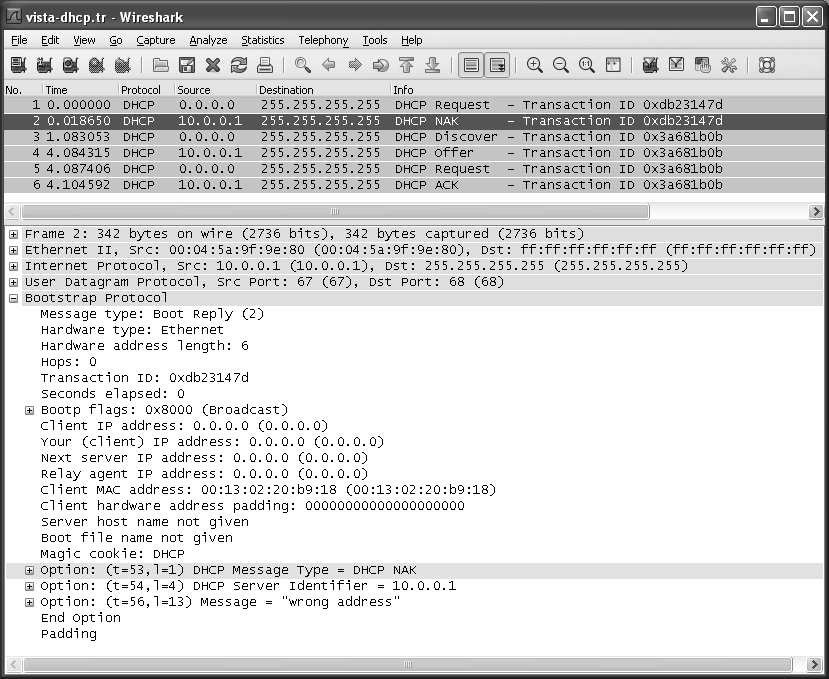
\includegraphics[scale=0.5]{imgs/6/6-4.png}
	\caption{一台客户机已切换网络,但它尝试通过 DHCPREQUEST 消息向新网络中的DHCP 服务器请求自己的旧地址 172.16.1.34}
\end{figure}

在图6-3中,我们可看到用链路层广播帧发送的DHCP 请求(目的地为ff:ff:ff:ff:ff.ff),
它使用未指定的源IP 地址0.0.0.0和受限的广播目的地址 255.255.255.255。由于客户机不知
道请求的地址是否成功分配,也不知道它连接的网络所使用的网络前缀,它将不得不使用这
些地址。这个消息是由 BOOTP 客户机的端口 68(bootpc)向服务器的端口 67(bootps)发送
的UDPAIP数据报。当DHCP作为BOOTP 的一部分时,使用的协议是引导程序协议,消息
类型是 BOOTREQUEST(1),硬件类型设置为1(以太网),地址长度为6字节。事务ID 为
0xdb23147d,它是由客户机选择的一个随机数。这个消息中设置了 BOOTP广播标志,意味
着该消息的响应通过广播地址发送。请求的地址172.16.1.34包含在几个选项之一中。我们
将在 6.2.9节详细介绍 DHCP 消息中出现的选项类型。

附近的DHCP 服务器会接收到客户机的DHCPREOUEST 消息,其中包括请求的IP地
址172.16.1.34。但是,服务器无法分配这个地址,这是由于172.16.1.34不在当前网络中
因此,服务器将会发送一个 DHCPNAK 消息,拒绝客户机的请求(见图 6-4)。

\begin{figure}[H]
    \centering
	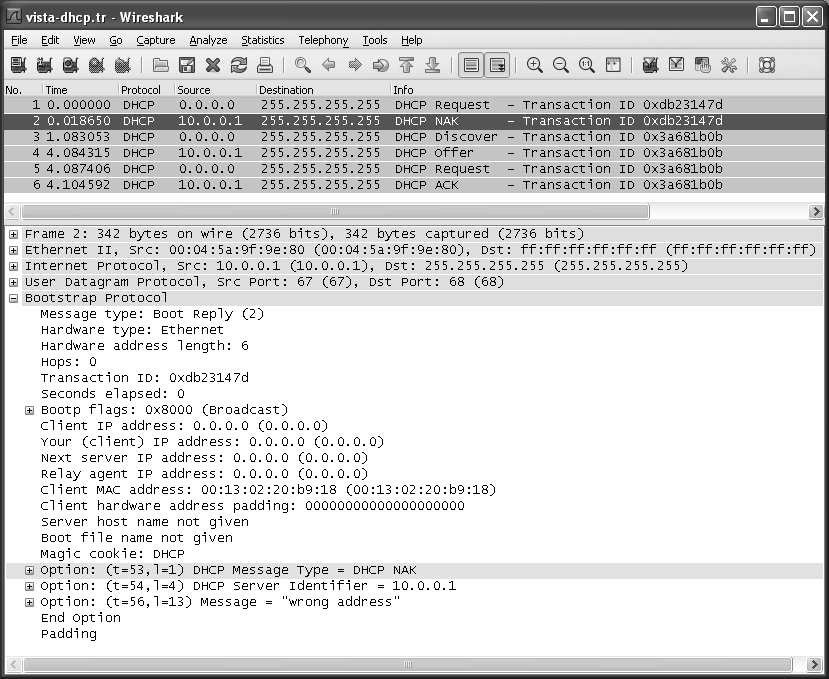
\includegraphics[scale=0.5]{imgs/6/6-4.png}
	\caption{DHCP服务器发送一个 DHCPNAK 消息,表示客户机不应尝试使用 IP 地址 172.16.1.34。事务ID 使客户机知道该消息对应的地址请求}
\end{figure}

图6-4所示的DHCPNAK消息是服务器发送的一个广播BOOTP响应。它包括
DHCPNAK消息类型、与客户机请求匹配的事务ID、包含10.0.0.1 的服务器标识符选
项、客户机标识符(在这种情况下是MAC地址)的副本,以及一个表示错误类型的文
本字符串“wrong address”。此后,客户机不再使用旧地址172.16.1.34,而是通过一个
DHCPDISCOVER 消息(见图6-5)重新寻找它能找到的服务器和地址。

客户机发送的DHCPDISCOVER 消息如图6-5所示,它与DHCPREQUEST 消息相似,
包括之前使用的已请求的IP地址(它没有任何其他要请求的地址),但包含了更丰富的选项
和一个新的事务ID(0x3a681b0b)。除了客户机 MAC地址出现在客户机硬件地址(chaddr)
字段中,大多数主要的 BOOTP 字段保留空并设置0。注意,这个地址如预期那样与以太
网帧的源 MAC地址匹配,这是由于分组并不通过BOOTP 中继代理来转发。DISCOVER 消
息的其他部分包含8个选项,其中大部分在图6-6的屏幕截图中展开了,因此我们可看到多
个选项的子类型。

图6-6给出了BOOTP请求消息中包含的选项。第一个选项表示该消息是一个
DHCPDISCOVER 消息。第二个选项表示客户机是否采用地址自动配置\href{https://www.rfc-editor.org/rfc/rfc2563}{\href{https://www.rfc-editor.org/rfc/rfc2563}{[RFC2563]}}(见 6.3
节)。如果不能通过DHCP 获取地址,则允许它自己决定是否作为 DHCP服务器使用。

\begin{figure}[H]
    \centering
	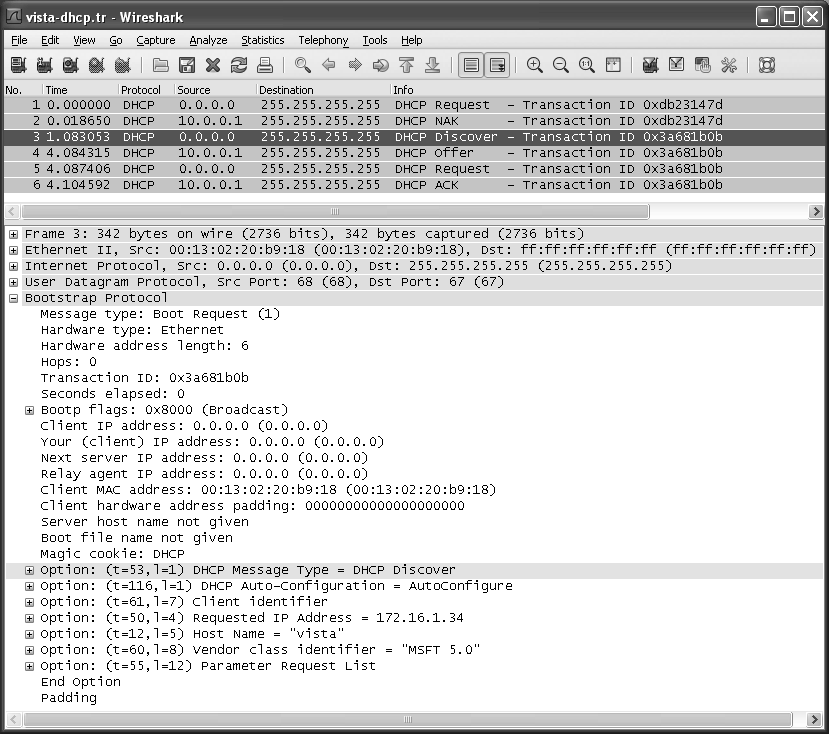
\includegraphics[scale=0.5]{imgs/6/6-5.png}
	\caption{DHCPDISCOVER 消息表明在之前的 DHCPREQUEST 消息失败后,客户机正在重新尝试获得一个地址}
\end{figure}

\begin{figure}[H]
    \centering
	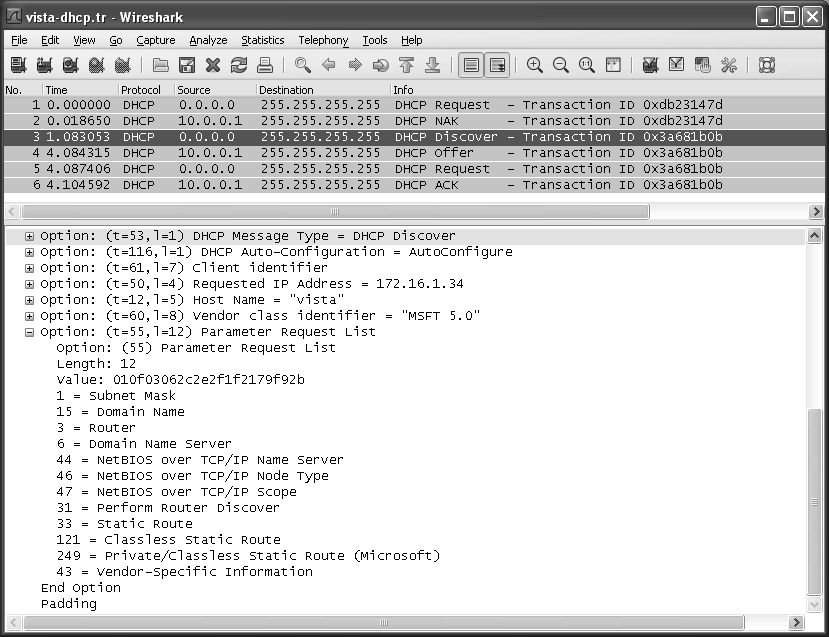
\includegraphics[scale=0.5]{imgs/6/6-6.png}
	\caption{DHCPDISCOVER 消息可能包含丰富的参数请求,说明客户机需要哪些配置信息}
\end{figure}

下一个选项表示客户机标识符(ID)选项设置为0100130220B918(未显示)。DHCP服
务器可使用客户机 ID,以确定是否有特殊配置信息给特定的客户机。目前,大多数操作系
统允许用户在获得一个地址时指定 DHCP 客户机使用的客户机 ID。但是,允许自动选择客
户机 ID 通常更便利,这是由于多个客户机使用相同客户机 ID 会导致DHCP问题。自动选择
的客户机 ID 通常基于客户机MAC地址。在 Windows 中,它是在 MAC地址前面添加一个1
字节的硬件类型标识符(在这种情况下,该字节的值为1,表示以太网)。

\begin{tcolorbox}
    这里出现使用客户机标识符的举动,该标识符并非基于MAC地址。这
    样做的目的是希望一台客户机拥有一个持久的标识符,它使用不变的IPV4或
    IPv6地址,即使系统中的网络接口硬件改变(通常会导致其MAC地址改变)。
    \href{https://www.rfc-editor.org/rfc/rfc4361}{\href{https://www.rfc-editor.org/rfc/rfc4361}{[RFC4361]}}指定了用于IPV4节点的标识符,它使用一种最初为IPV6定义的方
    菜。它涉及使用DHCP 唯一标识(DUID)和身份关联标识符(IAID),它们是为
    DHCPv6\href{https://www.rfc-editor.org/rfc/rfc3315}{\href{https://www.rfc-editor.org/rfc/rfc3315}{[RFC3315]}}(见6.2.5.3节和6.2.5.4节)定义的,但可用于传统 DHCPV4 中。
    它不支持在 DHCP 消息中使用客户机硬件地址(chaddr)字段。但是,这种方案还
    没有被广泛应用。
\end{tcolorbox}

下一个(请求的IP 地址)选项表示客户机请求的IP 地址172.16.1.34。这是它在以前
的无线网络中使用的IP地址。正如前面所述,这个地址在新的网络中无法使用,这是由于
它使用了不同的网络前缀。

其他选项指出了配置主机名“vista”、供应商类别ID“MSFT 5.0”(由 Microsoft
Windows 2000及更高版本系统使用)和一个参数请求列表。参数请求列表选项为DHCP服
务器提供客户机请求的配置信息。它包含一个由多个字节组成的字符串,每个字节表示一个
特定的选项号。我们可以看到,它包含传统 Internet 信息(子网掩码、域名、DNS服务器、
默认的路由器),而且还包含一些其他选项,常见的是针对 Microsoft 系统(即 NetBIOS)的
选项。它还包含一个标识,表明客户机有兴趣知道是否执行 ICMP 路由器发现(见第8章),
以及是否在启动时将静态转发表项添加在客户机的转发表中(见第5章)。

\begin{tcolorbox}
    存在三种静态路由参数是地址发展过程造成的。在全面采用子网掩码和网络
    前缀之前,一个地址的网络部分是需要单独检测的地址(“分类地址”),这是与静
    态路由(33)参数共同使用的路由形式。随着无类路由的使用,DHCP 更新以保持
    掩码可用,这导致了\href{https://www.rfc-editor.org/rfc/rfc3442}{\href{https://www.rfc-editor.org/rfc/rfc3442}{[RFC3442]}}定义的无分类静态路由(CSR)参数(121)的出
    现。微软的改进方案(使用代码249)与之相似。
\end{tcolorbox}

最后一个参数(43)是针对特定供应商的信息。它通常与供应商类别标识符选项(60)
共同使用,以便允许客户机接收非标准的信息。其他方案结合供应商身份与特定供应商信
息\href{https://www.rfc-editor.org/rfc/rfc3925}{\href{https://www.rfc-editor.org/rfc/rfc3925}{[RFC3925]}},提供一种由供应商提供特定信息的方法(即使只有一台客户机)。在采用
Microsoft 系统的情况下,特定供应商信息用于选择使用的 NeBIOS,指出一个 DHCP 租约
是否在关机时释放,以及如何衡量一条默认路由在转发表中的处理。它也可用于 Microsoft
网络访问保护(NAP)系统[MS-DHCPN]。Mac OS 系统使用供应商特定信息支持苹果
NetBoot 服务和引导服务器发现协议(BSDP) [F07]。

在接收一个 DHCPDISCOVER 消息后,DHCP 服务器会响应一个IP 地址、租约和其他
配置信息的确认,它们包含在一个 DHCPOFFER 消息中。在图6-7所示的例子中只有一台
DHCP 服务器(它也是路由器和 DNS服务器)。

\begin{figure}[H]
    \centering
	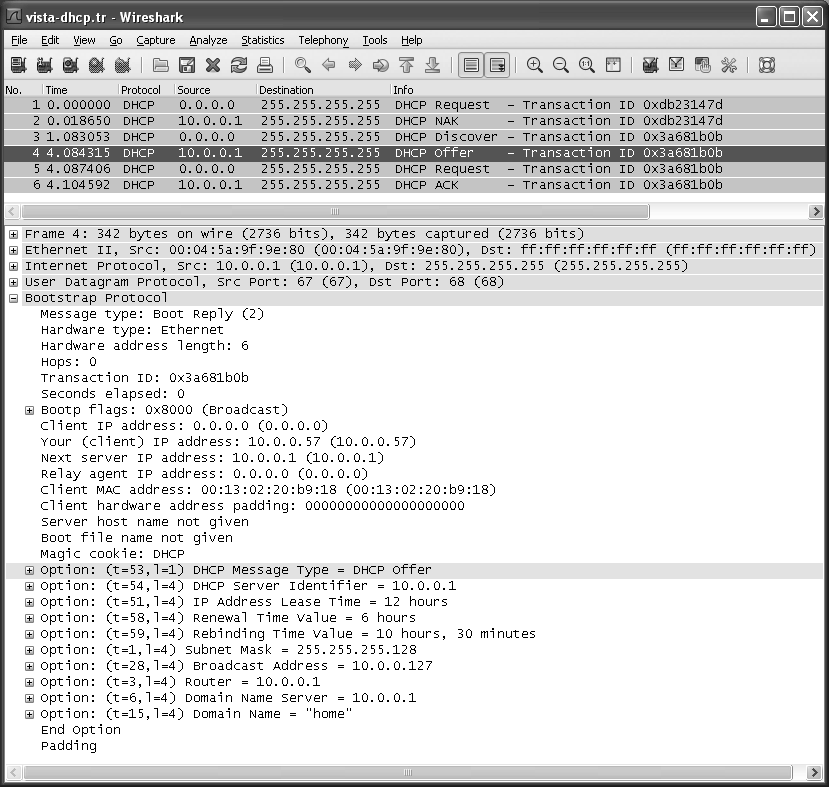
\includegraphics[scale=0.5]{imgs/6/6-7.png}
	\caption{10.0.0.1的DHCP服务器发送的 DHCPOFFER 提供有效期长达12小时的IP 地址10.0.0.57。其
    他信息包括 DNS服务器地址、域名、默认路由器的IP 地址、子网掩码和广播地址。在这个例
    子中,该系统是 IP 地址10.0.0.1 的默认路由器、DHCP 服务器和 DNS服务器}
\end{figure}

在图6-7所示的DHCPOFFER 消息中,我们再次看到消息格式中包含BOOTP 部分,以
及一组涉及DHCP地址处理的选项。BOOTP 消息类型是 BOOTREPLY。由服务器提供的客
户机 IP 地址为10.0.0.57,它位于“你的”[客户机]IP地址字段中。注意,该地址不匹配
DHCPDISCOVER 消息中包含的请求值 172.16.1.34,这是由于 172.16/12 前缀不能用于该本
地网络中。

包含在这组选项中的其他信息包括服务器的IP 地址(10.0.0.1)、提供的IP地址的租用
期(12小时)、T1(更新)和T2(重新绑定)的超时时间(分别为6h和10.5h)。另外,服务
器向客户机提供了子网掩码(255.255.255.128)、正确的广播地址(10.0.0.127)、默认路由
器和 DNS 服务器(均为10.0.0.1,与DHCP服务器一样)和默认域名“home”。该域名在格
式上不是标准的,并且不能用于专用网络之外。这个例子是一个家庭网络,采用作者常用的
<name>.home 格式的机器名。当客户机接收到一个 DHCPOFFER 消息,并决定租用服务岩
提供的 IP 地址10.0.0.57,它会发送第二个 DHCPREOUEST 消息(见图6-8)。

图 6-8
第二个 DHCPREQUEST 表示客户机希望使用IP 地址10.0.0.57。该消息通过广播地址来发送,
并在服务器标识符选项中包含地址10.0.0.1。这样任何其他服务器都可以接收广播,并且知道
客户机选择的 DHCP 服务器和地址

图6-8所示的第二个 DHCPREQUEST 消息与 DHCPDISCOVER消息类似,除了请求的
IP 地址现在设置为10.0.0.57,DHCP 消息类型设置为 DHCPREQUEST,DHCP 自动配置选项
不存在,服务器标识符选项现在已填充了服务器地址(10.0.0.1)。注意,与 DHCPDISCOVER
消息相似,这个消息采用广播方式发送,因此本地网络中的任何服务器或客户机都能接收
它。服务器标识符选项字段用于避免未选中的服务器提交地址绑定。当选中的服务器接收到
DHCPREQUEST 并同意绑定,它通常使用一个 DHCPACK 消息来响应,如图6-9所示。

图6-9所示的DHCPACK消息与前面的DHCPOFFER 消息非常相似。但是,客户机的
FQDN选项现在包括在内。在这种情况下(未显示),它被设置为vista.home。此后,客户机
免费使用地址10.0.0.57,直到 DHCP服务器失效为止。目前,建议使用ACD(在第4章中
描述) 技术,以确保地址不被其他主机使用。

当一个系统启动或连接到一个新的网络时,这个例子中交换的 DHCP 消息是典型的。它
也可能导致一个系统手工释放或获得 DHCP配置消息。例如,在 Windows 中,以下命令将
释放使用 DHCP 获得的数据:

C:\> ipconfig /release

下面的命令将获得数据:

C:> ipconfig /renew

\begin{figure}
    \centering
    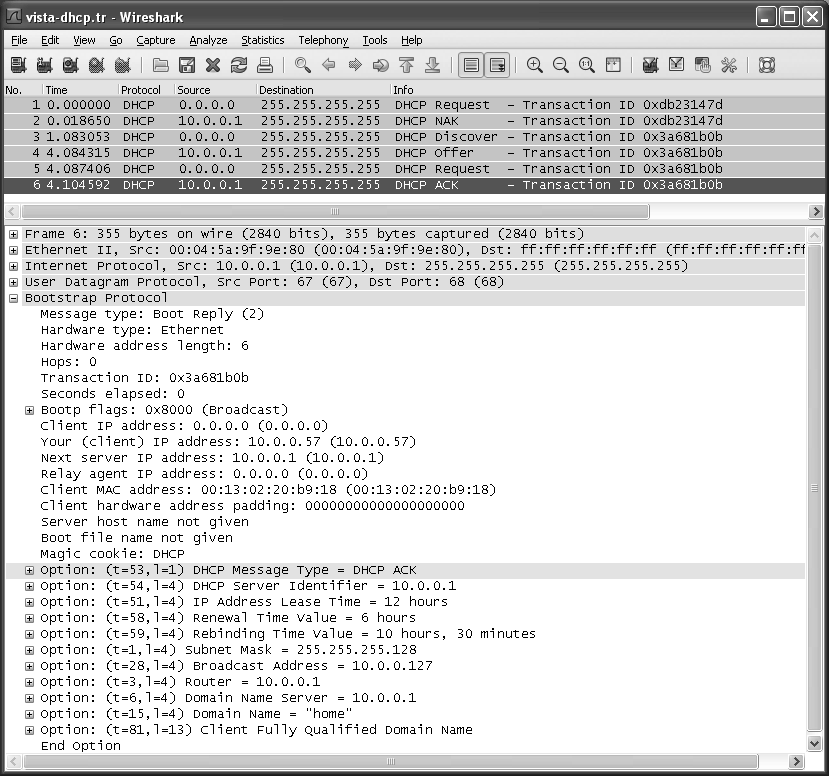
\includegraphics[scale=0.6]{imgs/6/6-9.png}
    \caption{DHCPACK 消息为客户机(和其他服务器)分配地址 10.0.0.57,其有效期长达12小时}
\end{figure}

在Linux 中,以下命令可获得同样结果:

\begin{verbatim}
    
Linux# dhclient -r
\end{verbatim}

释放一个租约,以及
\begin{verbatim}
Linux# dhclient
\end{verbatim}

更新一个租约。

通过DHCP 获得并分配给本地系统的信息类型,可在Windows 中通过一个ipc
选项来查看。下面是来自该命令的一段输出:

\begin{verbatim}
    
C:> ipconfig /a11

Wireless LAN adapter Wireless Network Connection:

Connection-specific DNS Suffix

Description

•

•:home

•

•

• :Intel(R)PRO/Wireless 3945ABG

Network Connection

Physical Address... .

••••:00-13-02-20-B9-18

DHCP Enabled.•

•••••Yes

Autoconfiguration Enabled

••••:Yes

IPV4 Address.....

••••:10.0.0.57(Preferred)

Subnet Mask••

•

••••:255.255.255.128

Lease Obtained...

•

•

...

•:Sunday,December

21,2008

11:31:48 PM

249

250

Lease Expires

•:Monday,December 22,2008

11:31:40 AM

Default Gateway

••:10.0.0.1

DHCP Server..

••

•

•

•

••:10.0.0.1

DNS Servers..

••••••:10.0.0.1

NetBIOS over Tcpip. •

•

••: Enabled

Connection-specific DNS Suffix Search List :home
\end{verbatim}

这个命令非常有用,可查看通过DHCP 或其他手段为主机分配的配置信息。

\subsection{DHCP状态机}

DHCP 协议在客户机和服务器中运行一个状态机。状态用于指出协议下一个处理的消息类
型。图6-10描述了客户机的状态机。状态之间的转换(箭头)源于消息的接收和发送或超时。

图6-10 DHCP 客户机的状态机。粗体的状态和转换通常涉及客户机首次获得租用地址。虚线和 INIT状
态表示协议开始

如图6-10所示,客户机开始于 INIT(初始)状态,这时没有信息,
并广播 DHCPDISCOVER 消息。在选择状态时,它接收 DHCPOFFER
消息,直到决定自己使用哪个地址和服务器。当它做出选择时,通过
一个 DHCPREQUEST 消息来响应,并进入请求状态。这时,它可能接
收来自不需要的地址的ACK。如果它没有发现需要的地址,发送一
个 DHCPDECLINE 消息,并转换到 INIT 状态。但是,更有可能出现的
情况是,它接收到一个自己需要的地址的DHCPACK 消息,接受它,
获得超时值T1 和T2,并进人绑定状态,这时就能使用这个地址直至
到期。当第一个计时器(T1)到期时,客户机进人更新状态并尝试重新
建立租约。如果它接收到一个新的 DHCPACK(客户机进入绑定状态),
这个过程成功。如果不成功,T2最终到期,并导致客户机尝试从任意服务器重新获得一个
地址。如果租用期最终到期,客户机必须放弃所租用的地址,如果没有可选的地址或可用的
网络连接,这时它将断开网络连接。

\subsection{DHCPV6}
虽然IPv4和IPv6的DHCP 协议希望实现类似目标,但它们各自的协议设计和部署选项
不同。DHCPv6\href{https://www.rfc-editor.org/rfc/rfc3315}{\href{https://www.rfc-editor.org/rfc/rfc3315}{[RFC3315]}} 可使用一种“有状态” 模式,其工作原理非常像DHCPV4,它也
可以使用一种“无状态”模式,并结合无状态地址自动配置(见6.3节)。在无状态模式下,
IPv6 客户机认为自己能配置IPv6地址,但需要通过DHCPv6 获得额外信息(例如 DNS服
务器地址)。另一种选择可使用ICMPv6 路由通告消息(见第8章、第11章和「RFC61061)
获得一台 DNS 服务器的位置。

\subsubsection{IPv6地址生命周期}

IPv6 主机的每个接口通常拥有多个地址,并且每个地址都拥有一组计时器,以指出相应
地址可使用多长时间和用于什么目的。在IPv6 中,地址分配包含一个首选生命周期和一个
有效生命周期。这些生命周期用于判断超时,将地址在自己的状态机中从一种状态转换为另
一种状态(见图6-11)。

图 6-11
IPv6地址的生命周期。临时地址仅用于 DAD,直至被验证为唯一。此后,它们成为首选地
址,并可无限制地使用,直至超时将其状态更改为废弃。废弃地址不能用于初始化新连接,
并且可能在有效超时期满后不能使用

图6-11给出了一个 IPv6地址的生命周期。当一个地址处于首选状态时,它可用于一般
用途,并可作为源或目的IPv6地址。当首选状态的超时到达时,相应的首选地址将废弃。当
该地址处于废弃状态时,它仍可用于现有传输(例如 TCP)连接,但不能用于启动新的连接。

当一个地址第一次被选择使用时,它进人一个临时或乐观状态。在处于临时状态时,它
可能仅用于IPv6邻居发现协议(见第8章)。这时,它不可用作任何其他目的的源或目的地
址。同时,该状态的地址要检测重复,看看同一网络中的其他节点是否已使用该地址。这个
过程称为重复地址检测(DAD),我们将在6.3.2.1 节详细介绍。常规 DAD 的替代方案称
乐观 DAD\href{https://www.rfc-editor.org/rfc/rfc4429}{\href{https://www.rfc-editor.org/rfc/rfc4429}{[RFC4429]}},通过它选择的地址可用于一组有限的用途,直至DAD完成。因为一
个乐观状态的地址实际上仅是针对 DAD 的一组特殊规则,它不是一个真正完整的状态。乐
观地址对大多数目的而言是废弃的。特别是,一个地址可能同时是乐观的和废弃的,这取决
于首选和有效生命周期。

\subsubsection{DHCPv6 消息格式}
DHCPv6消息封装为UDP/IPv6数据报,它使用客户机端口546和服务器端口547(见
第10章)。消息发送到中继代理或服务器,它使用一台主机的链路范围的源地址。这里存在
两种消息格式,一种用于客户机与服务器之间,另一种用于中继代理(见图6-12)。

图6-12左侧给出了基本 DHCPv6消息格式,右侧给出了一种扩展版本,其中包括链
路地址和对等方地址字段。右侧的格式用于 DHCPv6 中继代理和 DHCPv6 服务器之间。链
路地址字段给出了全局 IPv6地址,服务器用它标识客户机所处的链路。对等方地址字段包
含中继代理地址或客户机地址(要中继的消息来自该客户机)。注意,中继过程可能是链状
的,某个中继可能转发来自其他中继的消息。6.2.6节中描述了针对DHCPv4 和 DHCPv6 的
中继

图 6-12
基本 DHCPv6 消息格式(左)和中继代理消息格式(右)。
在DHCPv6中,最有意义的信息携带在选项中

左侧的消息格式中的消息类型包括典型的DHCP 消息(REQUEST、REPLY 等),右侧
的消息格式中的消息类型包括 RELAY-FORW 和 RELAY-REPL,分别表示从中继代理转发和
目的地是中继代理的消息。右侧的选项字段包括一个中继消息选项,其中包含中继转发的完
整消息。其他选项也可包含在内。

DHCPv4 和 DHCPv6之间的区别之一是 DHCPv6使用IPv6 组播地址的方式。客户机将请
求发送到所有 DHCP 中继代理和服务器的组播地址(ff02::1:2)。源地址在链路本地范围。在
IPv6 中,没有保留BOOTP 消息格式。但是,这个消息的语义类似。表6-1给出了 DHCPV6
的消息类型、取值和定义它的RFC,以及针对 DHCPv4 的同类消息和定义它的 RFC。

表6-1 DHCPv6消息的类型、值和标准。右侧给出了针对DHCPV4 的同类消息

DHCPV6 消息

DHCPV6值

参考文献

DHCPv4 消息

SOLICIT

ADVERTISE

REQUEST

CONFFIRM

RENEW

REBIND

REPLY

RELEASE

DECLINE

RECONFIGURE

INFORMATION-REQUEST

RELAY-FORW

RELAY-REPL

LEASEQUERY

\href{https://www.rfc-editor.org/rfc/rfc3315}{\href{https://www.rfc-editor.org/rfc/rfc3315}{[RFC3315]}}

DISCOVER

\href{https://www.rfc-editor.org/rfc/rfc3315}{\href{https://www.rfc-editor.org/rfc/rfc3315}{[RFC3315]}}

OFFER

\href{https://www.rfc-editor.org/rfc/rfc3315}{\href{https://www.rfc-editor.org/rfc/rfc3315}{[RFC3315]}}

REQUEST

\href{https://www.rfc-editor.org/rfc/rfc3315}{\href{https://www.rfc-editor.org/rfc/rfc3315}{[RFC3315]}}

REQUEST

\href{https://www.rfc-editor.org/rfc/rfc3315}{\href{https://www.rfc-editor.org/rfc/rfc3315}{[RFC3315]}}

REQUEST

\href{https://www.rfc-editor.org/rfc/rfc3315}{\href{https://www.rfc-editor.org/rfc/rfc3315}{[RFC3315]}}

DISCOVER

\href{https://www.rfc-editor.org/rfc/rfc3315}{\href{https://www.rfc-editor.org/rfc/rfc3315}{[RFC3315]}}

ACK/NAK

\href{https://www.rfc-editor.org/rfc/rfc3315}{\href{https://www.rfc-editor.org/rfc/rfc3315}{[RFC3315]}}

RELEASE

9

10

11

12

13

14

\href{https://www.rfc-editor.org/rfc/rfc3315}{\href{https://www.rfc-editor.org/rfc/rfc3315}{[RFC3315]}}

DECLINE

\href{https://www.rfc-editor.org/rfc/rfc3315}{\href{https://www.rfc-editor.org/rfc/rfc3315}{[RFC3315]}}

FORCERENEW

\href{https://www.rfc-editor.org/rfc/rfc3315}{\href{https://www.rfc-editor.org/rfc/rfc3315}{[RFC3315]}}

INFORM

\href{https://www.rfc-editor.org/rfc/rfc3315}{\href{https://www.rfc-editor.org/rfc/rfc3315}{[RFC3315]}}

N/A

\href{https://www.rfc-editor.org/rfc/rfc3315}{\href{https://www.rfc-editor.org/rfc/rfc3315}{[RFC3315]}}

N/A

\href{https://www.rfc-editor.org/rfc/rfc5007}{\href{https://www.rfc-editor.org/rfc/rfc5007}{[RFC5007]}}

LEASEQUERY

LEASE{UNASSIGNED,

LEASEQUERY-REPLY

15

\href{https://www.rfc-editor.org/rfc/rfc5007}{\href{https://www.rfc-editor.org/rfc/rfc5007}{[RFC5007]}}

UNKNOWN, ACTIVE}

LEASEQUERY-DONE

LEASEQUERY-DATA

N/A

16

17

N/A

\href{https://www.rfc-editor.org/rfc/rfc5460}{\href{https://www.rfc-editor.org/rfc/rfc5460}{[RFC5460]}}

\href{https://www.rfc-editor.org/rfc/rfc5460}{\href{https://www.rfc-editor.org/rfc/rfc5460}{[RFC5460]}}

N/A

LEASEQUERYDONE

N/A

BULKLEASEQUERY

参考文献

\href{https://www.rfc-editor.org/rfc/rfc2132}{\href{https://www.rfc-editor.org/rfc/rfc2132}{[RFC2132]}}

\href{https://www.rfc-editor.org/rfc/rfc2132}{\href{https://www.rfc-editor.org/rfc/rfc2132}{[RFC2132]}}

\href{https://www.rfc-editor.org/rfc/rfc2132}{\href{https://www.rfc-editor.org/rfc/rfc2132}{[RFC2132]}}

\href{https://www.rfc-editor.org/rfc/rfc2132}{\href{https://www.rfc-editor.org/rfc/rfc2132}{[RFC2132]}}

\href{https://www.rfc-editor.org/rfc/rfc2132}{\href{https://www.rfc-editor.org/rfc/rfc2132}{[RFC2132]}}

\href{https://www.rfc-editor.org/rfc/rfc2132}{\href{https://www.rfc-editor.org/rfc/rfc2132}{[RFC2132]}}

\href{https://www.rfc-editor.org/rfc/rfc2132}{\href{https://www.rfc-editor.org/rfc/rfc2132}{[RFC2132]}}

\href{https://www.rfc-editor.org/rfc/rfc2132}{\href{https://www.rfc-editor.org/rfc/rfc2132}{[RFC2132]}}

\href{https://www.rfc-editor.org/rfc/rfc2132}{\href{https://www.rfc-editor.org/rfc/rfc2132}{[RFC2132]}}

\href{https://www.rfc-editor.org/rfc/rfc3203}{\href{https://www.rfc-editor.org/rfc/rfc3203}{[RFC3203]}}

\href{https://www.rfc-editor.org/rfc/rfc2132}{\href{https://www.rfc-editor.org/rfc/rfc2132}{[RFC2132]}}

\href{https://www.rfc-editor.org/rfc/rfc4388}{\href{https://www.rfc-editor.org/rfc/rfc4388}{[RFC4388]}}

\href{https://www.rfc-editor.org/rfc/rfc4388}{\href{https://www.rfc-editor.org/rfc/rfc4388}{[RFC4388]}}

[ID4LQ]

N/A

[ID4LQ]

在 DHCPv6 中,最有意义的信息携带在选项中,包括地址、租用时间、服务位置,以及
客户端标识符和服务器标识符。这些选项使用的两个重要概念是身份关联(IA)和 DHCP唯
一标识符(DUID)。我们将在后面加以讨论。

\subsubsection{身份关联}
身份关联(IA)是用在DHCP 客户机和服务器之间的一个标识符,用于指向一个地址
集。每个IA 包括一个IA 标识符(IAID)和相关配置信息。每个请求 DHCPv6 分配地址的客
户机接口至少需要一个IA。每个IA 可以仅与一个接口相关联。客户机选择的IAID 唯一地
标识每个IA,并将这个值与服务器共享。

IA 相关的配置信息包括一个或多个地址,以及相关的租约信息(T1、T2和总的租用时
间值)。IA的每个地址都有一个首选的和一个有效的生命周期\href{https://www.rfc-editor.org/rfc/rfc4862}{\href{https://www.rfc-editor.org/rfc/rfc4862}{[RFC4862]}},它定义了地址的
整个生命周期。请求的地址类型可以是常规地址或临时地址\href{https://www.rfc-editor.org/rfc/rfc4941}{\href{https://www.rfc-editor.org/rfc/rfc4941}{[RFC4941]}}。临时地址由随机数
的一部分派生而来,用于协助改善IPv6 主机地址跟踪的隐私问题。临时地址通常与非临时
地址同时分配,但需要频繁使用不同的随机数重新生成。

当服务器响应一个请求时,它客户机的IA 分配一个或多个地址,分配时基于服务器
管理员确定的一组地址分配策略。在通常情况下,这些策略依赖于请求所到达的链路、客
户机的标准信息(见6.2.5.4节的DUID),以及DHCP选项中由客户机提供的其他信息。
图6-13给出了非临时地址和临时地址的IA 选项格式。

0

1516

310

1516

31

OPTION\_IA\_NA

选项长度

OPTION\_IA\_TA

选项长度

IAID(4字节)

T1

T2

IA\_NA 选项

(可变)

针对非临时地址选项的IA

IAID(4字节)

IA\_TA 选项

(可变)

针对临时地址选项的IA

图 6-13
非临时地址(左)和临时地址(右)的DHCPv6 IA 格式。每个选项可能包括额外的选项,以
便描述特定 IPv6 地址和相应的租约

如图6-13所示,对于非临时地址和临时地址的IA选项,主要区别是非临时地址包括
T1 和T2值。这些值是已知的,它们也是DHCPv4使用的值。对于临时地址,可能缺少T1
和T2,因为生命周期通常基于分配给非临时地址的T1 和T2值确定,这些值之前是已知的。
\href{https://www.rfc-editor.org/rfc/rfc4941}{\href{https://www.rfc-editor.org/rfc/rfc4941}{[RFC4941]}}给出了临时地址的细节。

\subsection{ DHCP 唯一标识符}

DHCP 唯一标识符(DUID)用于标识一台 DHCPv6 客户机或服务器,并被设计为可持
续一段时间。服务器用它标识所选地址(作为IA 的一部分)对应的客户机和配置信息,客户
机用它标识感兴趣的服务器。DUID 长度是可变的,对于大多数用途来说,客户机和服务器
将它看作一个不透明的值。

DUID 是全球唯一的,但它很容易生成。为了同时满足这些关系,「RFC33151定义了三
种可能的DUID 类型,但也不是只能创建这三种类型。三种 DUID 类型如下:

1)DUID-LLT:基于链路层地址和时间的 DUID。
2) DUID-EN:基于企业编号和供应商分配的 DUID。
3) DUID-LL:仅基于链路层地址的 DUID。

一个标准格式的DUID编码开始于一个2字节的标识符,用于指出是哪种类型的
DUID。当前列表由IANA维护[ID6PARAM]。在 DUID-LLT 和 DUID-LL 中,紧跟着是一个
来自[RFCO826]的16位的硬件类型;在DUID-EN 中,则是一个32位的专用企业编号。

\begin{tcolorbox}
    专用企业编号(PEN)是一个32位的值,它由IANA 分配给一个企业。它通
    常与 SNMP 协议共同用于网络管理目的。到2011年中期,已分配大约38000个编
    号。当前列表可从IANA 获得[IEPARAM]。
\end{tcolorbox}

第一种格式的 DUID(即 DUID-LLT)是推荐的格式。在硬件类型之后,它包括一个32
位的时间戳,其中的秒数开始于2000年1月1日午夜(UTC)(mod 222)。它将在2136年归
零(返回0)。最后部分是一个可变长度的链路层地址。链路层地址可由任何主机接口选择,
并使用相同的 DUID,一旦选定,它可用于与任何接口的通信。这种格式的DUID 是稳定的,
即使网络接口从该 DUID 中移除。因此,它需要主机系统固定存储相关信息。DUID-LL 格式
非常相似,但推荐给缺少固定存储(但有一个固定的链路层地址)的系统。RFC指出 DUID.
LL 不能用于某些客户机或服务器,它们不能确定自己使用的链路层地址是否与一个可删除
的接口有关。

\subsubsection{协议操作}
DHCPv6协议操作与 DHCPv4 的对应部分相似。一台客户机是否启用 DHCP,取决于这
台主机接收的ICMPv6路由器通告消息中的配置选项(见第8章)。路由器通告包括两个重要
的位字段。M位是可管理地址配置标志,表示IPv6地址可使用DHCPv6 获得。0位是其他
配置标志,表示 IPv6地址之外的其他信息可使用DHCPv6 获得。这两个字段和其他字段定
义在\href{https://www.rfc-editor.org/rfc/rfc5175}{\href{https://www.rfc-editor.org/rfc/rfc5175}{[RFC5175]}}中。M 和O位字段可以任意组合,但M启用和O关闭可能是最不实用的组
合。如果两者都关闭,则不使用DHCPv6,并在分配地址时使用无状态地址自动分配(见6.3
节)。M关闭和O启用表示客户机使用无状态 DHCPv6,并使用无状态地址自动配置获得地
址。DHCPv6协议操作使用表6-1定义的消息,如图6-14所示。

在通常情况下,一台客户机首先确定使用的链路本地地址,然后执行ICMPV6 路由
器发现操作(见第8章),以确定所在网络中是否存在一台路由器。路由器通告包括前面
提到的M和O位字段。如果正在使用DHCPv6,则至少设置M位字段,并且由客户机来
组播(见第9章)DHCPSOLICIT消息,以便发现 DHCPv6服务器。如果存在一个或多个
DHCPADVERTISE 响应消息,表示至少存在一台 DHCPv6服务器。这些消息由2次称为四
消息交换的 DHCPv6操作构成。

在已知一台 DHCPv6服务器位置,或不需要分配地址(例如无状态 DHCPv6 或使用快
速确认选项,见6.2.9节)的情况下,“四消息交换”可简化为“两消息交换”,在这种情况
下只使用请求和应答消息。DHCPv6 服务器确认 DUID、IA 类型(临时、非临时或前缀,见
6.2.5.3节)和IAID结合而成的绑定。IAID 是由客户机选择的一个32位数字。每个绑定可
以有一个或多个租约,一个或多个绑定可通过一个 DHCPv6 事务来处理。

图 6-14
DHCPv6的基本操作。客户机通过ICMPv6路由器通告中的信息决定是否使用DHCPV6。如
果使用,DHCPv6 操作与 DHCPv4 相似,但在细节上有显著不同

\subsubsection{扩展的例子}

图6-15给出了一个例子,一台 Windows Vista (Service Pack 1)机器连接到一个无线网
络。它的IPv4 协议栈已被禁用。它首先分配自己的链路本地地址,并检查该地址是否已被
使用。

在图6-15中,我们看到ICMPv6邻居请求(DAD)为客户机分配的乐观地址为
fe80::fd26:de93:5ab7:405a。(我们在6.3.2.1节讨论无状态地址自动配置时,详细描述了
DAD。)分组发送到对应的目的节点地址 ff02::1:ffb7:405a。它乐观地假设该地址没有在链路
上使用,因此它立即发送一个路由器请求(RS)(见图6-16)。

图6-16中所示的RS发送到所有路由器的组播地址 ff02::2。这导致网络中的每台路由器
都响应一个路由器通告(RA),其中携带重要的M位和O位,客户需要通过它们来决定下一
步怎样做。

\begin{tcolorbox}
    这个例子显示了从乐观地址发送的一个路由器请求,其中包括一个源链路层
    地址选项(SLLAO),这违反了\href{https://www.rfc-editor.org/rfc/rfc4429}{\href{https://www.rfc-editor.org/rfc/rfc4429}{[RFC4429]}}中的规定。这里的问题是对任何处于侦
    听状态的IPv6路由器邻居缓存的潜在污染。它们将处理这个选项,并在自己的邻
    居缓存中建立临时地址和链路层地址之间的映射,这可能重复。但是,这种情况通
    常很少发生,并且不怎么被关注。尽管如此,如果待定的“乐观”选项[IDDN]是
    标准的,将允许路田器请求包含一个用于避免此问题的 SLLAO。
\end{tcolorbox}


\begin{figure}[H]
    \centering
	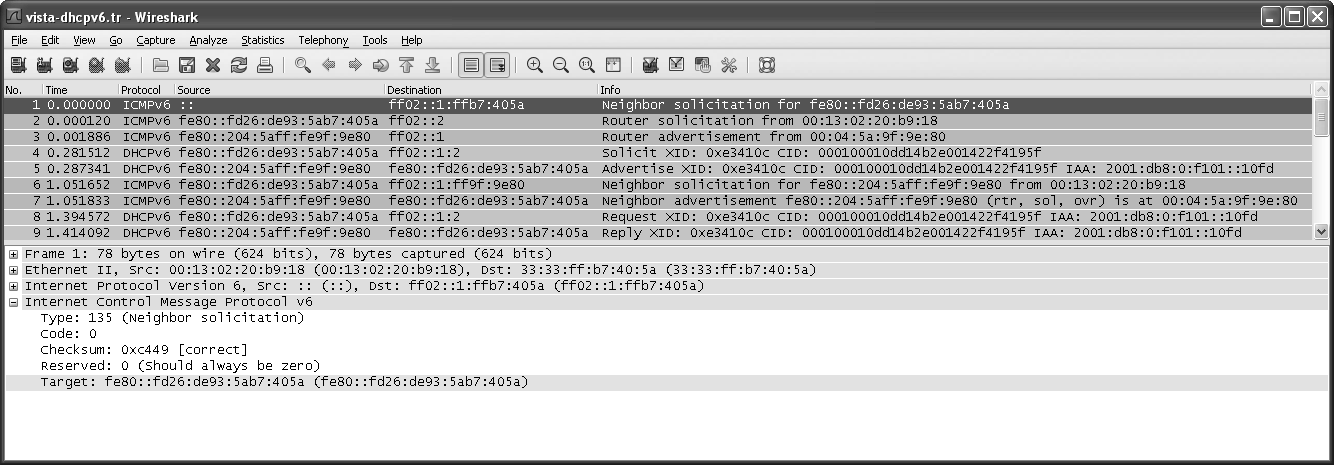
\includegraphics[scale=0.5]{imgs/6/6-15.png}
	\caption{10.0.0.1的DHCP服务器发送的 DHCPOFFER 提供有效期长达12小时的IP 地址10.0.0.57。其
    他信息包括 DNS服务器地址、域名、默认路由器的IP 地址、子网掩码和广播地址。在这个例
    子中,该系统是 IP 地址10.0.0.1 的默认路由器、DHCP 服务器和 DNS服务器}
\end{figure}


\begin{figure}[H]
    \centering
	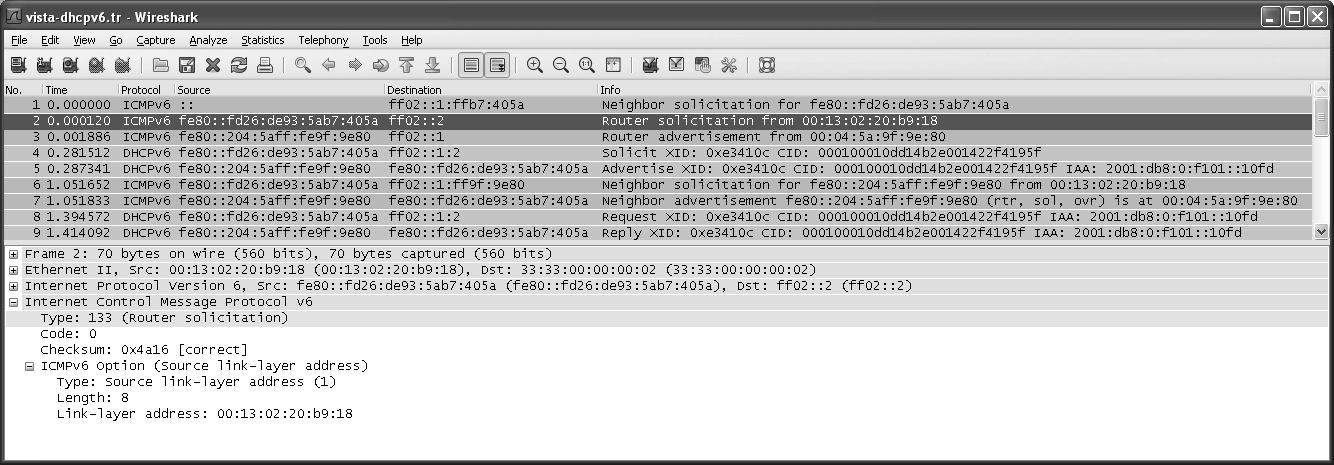
\includegraphics[scale=0.5]{imgs/6/6-16.png}
	\caption{路由器请求导致一台临近的路由器发送了一个路由器通告。请求消息被发送到所有路由器地址(ff02::2)}
\end{figure}

图6-17中的RA表示一台路由器存在,包括00:04:5a:9f:9e:80的 SLLAO,它对客户
机封装目的地为该路由器的后续链路层帧是有用的。标志字段表示M位和O位字段都启用
(设置为1),因此客户机应继续使用DHCPv6,以便获得自己的地址和其他配置信息。这个
过程通过请求一台 DHCPv6服务器来完成(见图6-18)。

\begin{figure}[H]
    \centering
	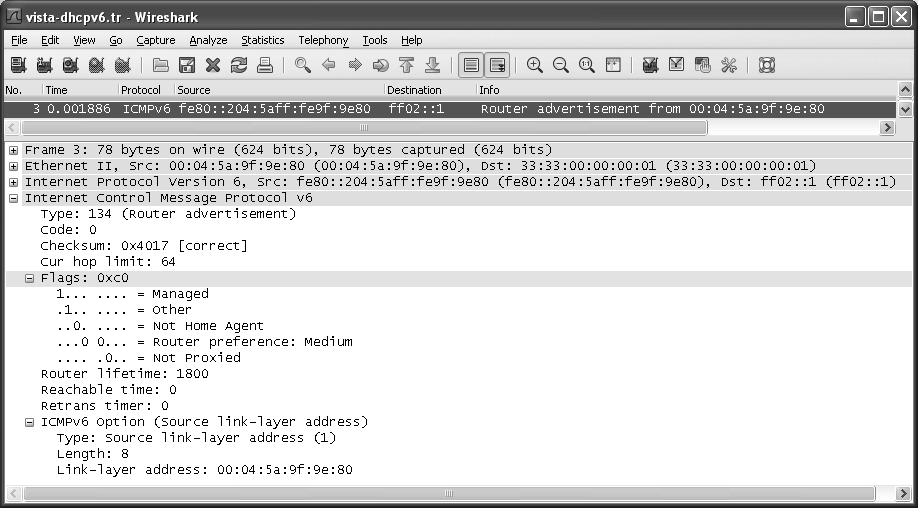
\includegraphics[scale=0.5]{imgs/6/6-17.png}
	\caption{一个路由器通告指出地址可被管理(可使用DHCPv6分配),以及可使用DHCPv6 获得的
    其他信息(例如DNS服务器)。这个网络使用有状态 DHCPv6。IPv6路由器通告消息使用
    ICMPv6(见第8章)}
\end{figure}

图6-18中显示了 DHCPv6 SOLICIT 消息,其中包括事务 ID(与DHCPv4 相似)、经历
的时间(0,图中未显示),以及一个包含时间和6字节MAC地址的DUID。在这个例子中,
MAC地址 00:14:22:f4:19:5f是这台客户机的有线以太网接口MAC地址,它不是用来发送
SOLICIT 消息的接口。回想 DUID-LL 和 DUID-TLL 类型的 DUID,其中的链路层信息对不
同接口应该是一样的。IA是一个非临时的地址,并且客户机已选择IAID 为09001302。这个
请求中的时间值为0,意味着客户机没有特定的期望,它们将由服务器来决定。

下一个选项是\href{https://www.rfc-editor.org/rfc/rfc4704}{\href{https://www.rfc-editor.org/rfc/rfc4704}{[RFC4704]}}规定的FQDN选项。它用于携带客户机的FQDN,但会影响
DHCPv6 和DNS之间的交互(见6.4节中的DHCP 和DNS交互)。这个选项用于启用由客户
机或服务器动态更新的FQDN 到IPv6地址的映射。(反向通常由服务器来处理。)这个选项的
第一部分包含3位:N(服务器不执行更新)、O(服务器忽略客户机请求)和S(服务器执行
更新)。这个选项的第二部分包含一个域名,它可能是完全限定域名,也可能不是。

\begin{tcolorbox}
    Wireshark 工具显示图6-18中记录的FQDN名称异常,并推测该分组可能是
    由一个 MS Vista 客户机生成的。字段异常的原因是这个选项的最初规范允许使用
    ASCII 字符编码的简单域名。这种方法在\href{https://www.rfc-editor.org/rfc/rfc4704}{\href{https://www.rfc-editor.org/rfc/rfc4704}{[RFC4704]}}中已被废弃,并且两种编码不
    直接兼容。微软提供了一个修补程序,为 Vista 系统解决这个问题。微软 Windows
    7系统的行为符合「RFC47041。
\end{tcolorbox}

\begin{figure}[H]
    \centering
	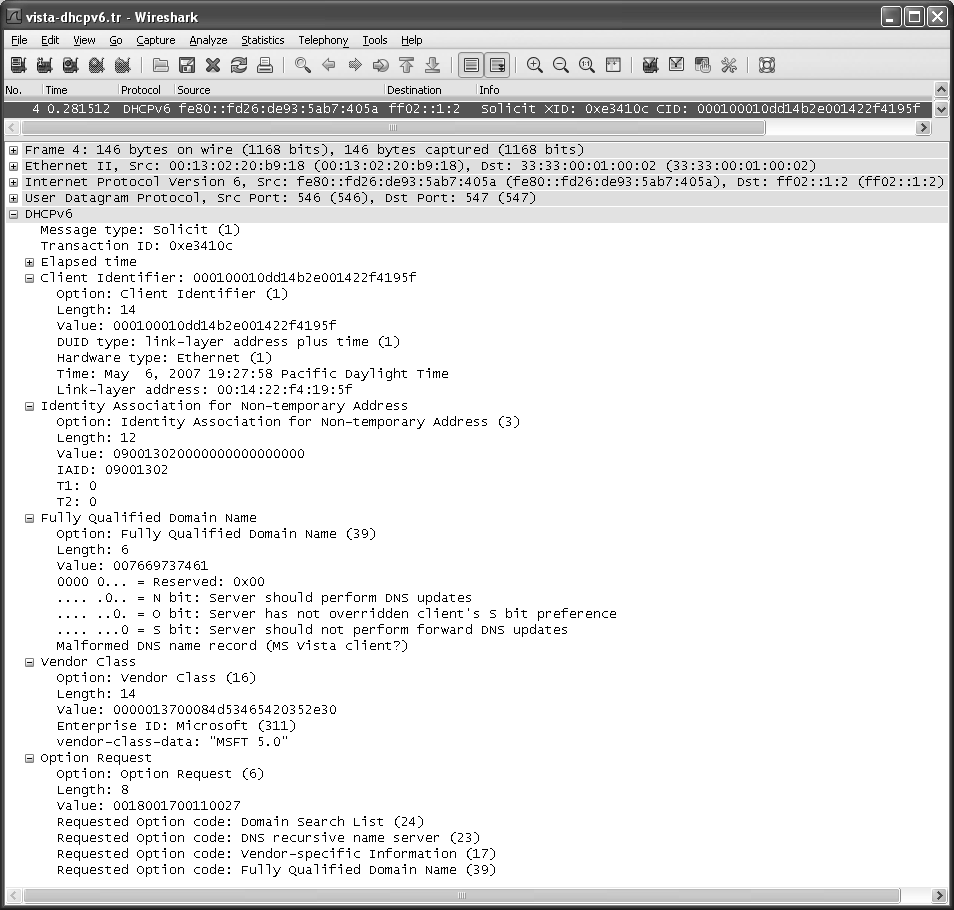
\includegraphics[scale=0.5]{imgs/6/6-18.png}
	\caption{DHCPv6 SOLICIT 消息请求一个或多个 DHCPv6服务器的位置,以及用于识别客户机的信息和它感兴趣的选项}
\end{figure}

请求消息中的其他信息包括供应商类别标识符和请求选项列表。在这种情况下,供应商
类别数据包括字符串“MSFT 5.0”,它可由一台 DHCPv6 服务器使用,以确定客户机能进行
哪些类型的处理。为了响应客户机的请求,服务器响应一个通告消息(见图 6-19)。

图6-19所示的ADVERTISE 消息为客户机提供了更多信息。客户机标识符选项与客户
机配置信息相呼应。服务器标识符选项给出了一个时间和一个链路层地址 10:00:00:00:09:20
来标识服务器。IA拥有一个IAID值09001302(由客户机提供),并包括一个全球地址
2001:db8:0:f101:10fd,其首选生命周期和有效生命周期分别为130s和200s(超时时间相
当短)。状态码为0表示成功。与DHCPv6通告一起提供的还有DNS递归名称服务器选项
\href{https://www.rfc-editor.org/rfc/rfc3646}{\href{https://www.rfc-editor.org/rfc/rfc3646}{[RFC3646]}},它指出一个服务器地址 2001:db8:0:f101::1 和一个包含home 字符串的域名搜索
列表选项。注意,服务器并不包括FQDN 选项,这是由于它不需要执行这个选项。

下面两个分组是常规的邻居请求和邻居通告消息,它们在客户机与路由器之间交
换,我们不会进一步描述它们。这个交换开始于客户机请求确认一个全球非临时地址
2001:db8:0:f101::10fd(见图6-20)。

\begin{figure}[H]
    \centering
	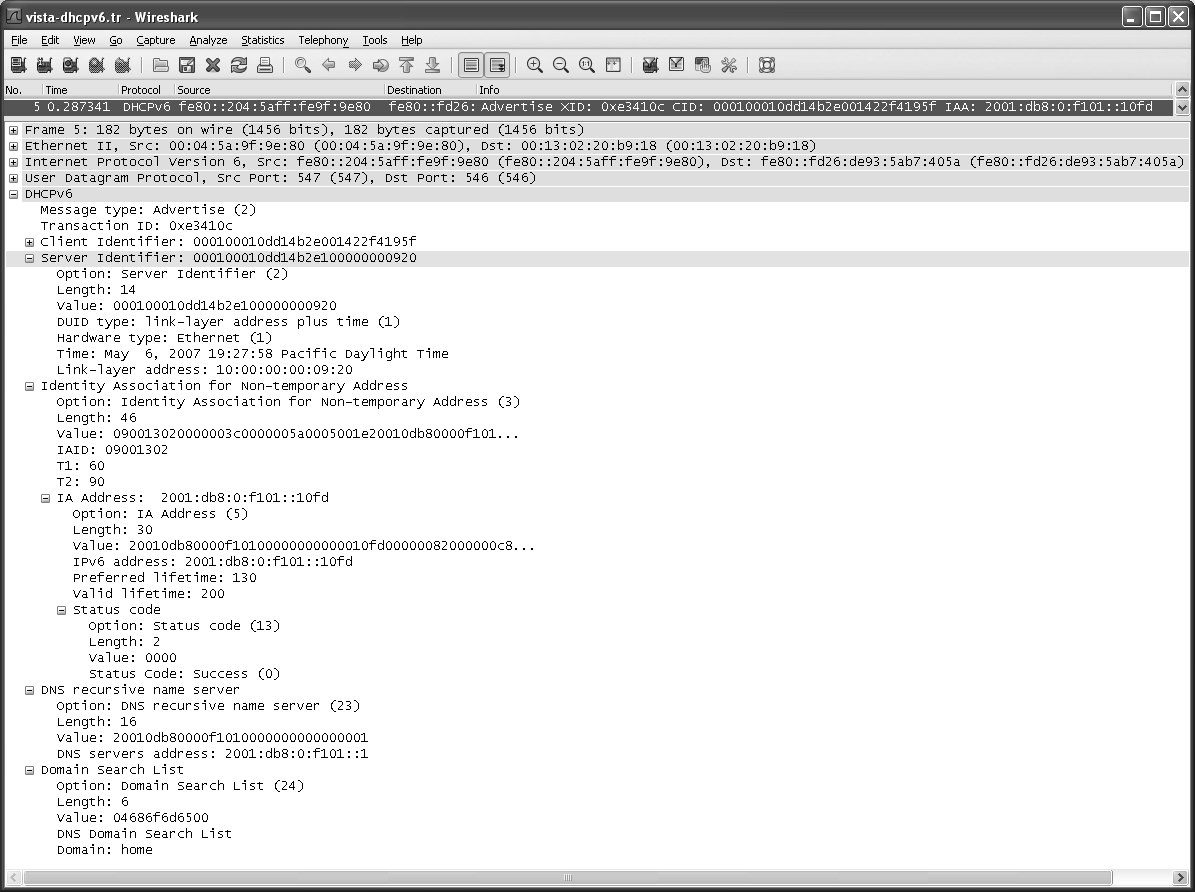
\includegraphics[scale=0.5]{imgs/6/6-19.png}
	\caption{DHCPv6 ADVERTISE 消息包括地址、租约,以及 DNS服务器的IPv6地址和域名搜索列表}
\end{figure}

\begin{figure}[H]
    \centering
	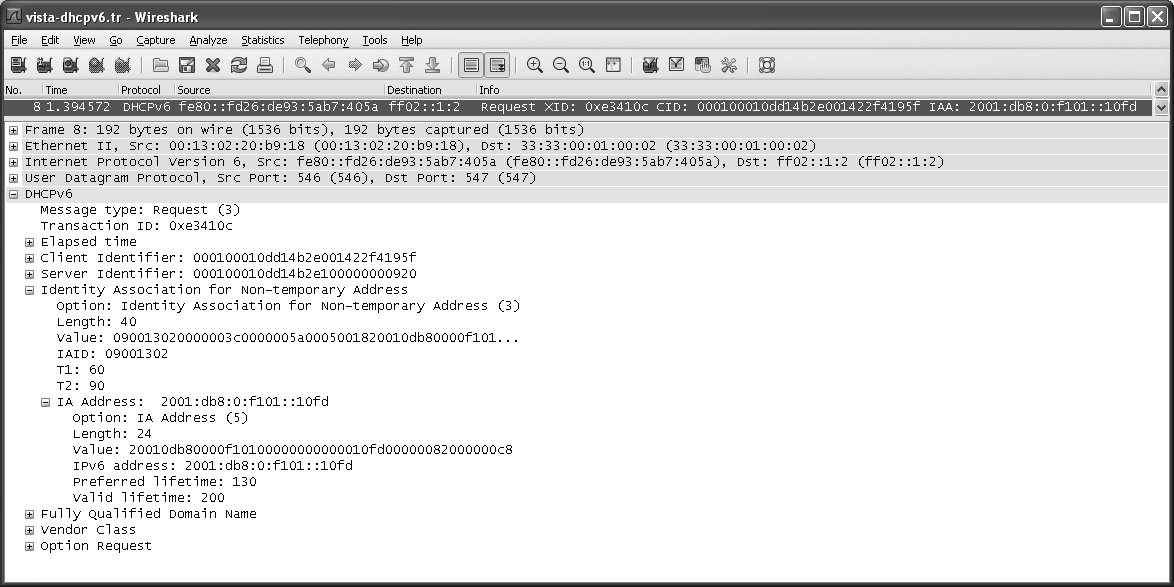
\includegraphics[scale=0.5]{imgs/6/6-20.png}
	\caption{DHCPV6 REQUEST 消息与SOLICIT 消息相似,但它包含从
    服务器 ADVERTISE 消息中学习到的信息}
\end{figure}

图6-20所示的 REQUEST 消息与SOLICIT 消息相似,但它包含来自服务器的 ADVERTISE
消息中携带的信息(地址及T1和T2值)。我们看到的所有 DHCPv6消息中的事务ID 相同。
这个交换通过 REPLY 消息完成,它与ADVERTISE 消息除了消息类型不同之外其余都相同,
因此这里不再详细介绍。

在重启一个系统和连接到一个新的网络时,这个例子中交换的DHCPv6 消息是典型的。
在DHCPv4中,它可能导致一个系统手工释放或获得信息。例如,在 Windows 中,以下命
令使用 DHCPv6 释放获得的数据:

\begin{verbatim}
    C:\> ipconfig /release6
\end{verbatim}

以下命令用于获得它:

\begin{verbatim}
    C:> ipcontig /renew6
\end{verbatim}

通过 DHCP 获得并分配给本地接口的信息类型,可使用之前看过的该命令的另一个选项
来查看。下面是其输出的一部分:
\begin{verbatim}
    C:\> ipconfig /a11

Wireless LAN adapter Wireless Network Connection:

Connection-specific DNS Suffix • :home

Description• .

••: Intel(R) PRO/Wireless 3945ABG

Network Connection

Physical Address.

DHCP Enabled.

Autoconfiguration Enabled

IPv6 Address.••

Lease Obtained.

••:00-13-02-20-B9-18

••: Yes

••••:Yes

• •: 2001:db8:0:f101::12cd(Preferred)

••:Sunday,December 21,2008

11:30:45 PM

Lease Expires

••:Sunday,December 21,2008

11:37:04 PM

Link-local IPv6 Address

••:

fe80::fd26:de93:5ab7:405a89(Preferred)

Default Gateway .

DHCPv6 IAID

••

DHCPv6 Client DUID.

••: fe80::204:5aff:fe9f:9e8089

••:150999810

••:

00-01-00-01-0D-D1-4B-2E-00-14-22-F4-19-5F

DNS Servers

••:2001:db8:0:f101::1

NetBIOS over Tcpip. .

••: Disabled

Connection-specific DNS Suffix Search List :

home

\end{verbatim}
这里,我们可以看到该系统的链路层地址(00:13:02:20:b9:18)。注意,在这个例子中,
该地址从未作形成IPv6 地址的基础而使用。

\subsubsection{DHCPv6 前缀委托(DHCPV6-PD 和ord)}
目前为止的讨论围绕着配置主机,但 DHCPv6也可用于配置路由器。这通过一台路由器
向另一台路由器委托一个地址空间范围来实现。这个地址范围可描述为一个 IPv6地址前缀。
这个前缀在\href{https://www.rfc-editor.org/rfc/rfc3633}{\href{https://www.rfc-editor.org/rfc/rfc3633}{[RFC3633]}}定义的DHCP 前缀选项中。这用于路由器委托的情况,它现在可像一
个 DHCPv6 服务器那样工作,而不需要前缀网络的详细拓扑信息。这种情况可能发生,例如
ISP给出了一个可由潜在客户重新分配的地址范围。在这种情况下,ISP 可能使用 DHCPV6-
PD 向客户设备委托一个前缀。

前缀委托定义了一种新格式的IA,称为IA\_PD。每个IA\_PD 由一个IAID 和相关的配
置信息构成,它在地址上与前面讨论的IA相似。DHCPv6-PD 不只对固定路由器的前缀委托
有用,它也可用于移动路由器(及其连接的子网)[RFC62761。

目前,已创建一种特殊格式的PD(6rd,见\href{https://www.rfc-editor.org/rfc/rfc5569}{\href{https://www.rfc-editor.org/rfc/rfc5569}{[RFC5569]}})以支持服务提供商快速部署
IPv6。在 OPTION\_6RD(212)选项\href{https://www.rfc-editor.org/rfc/rfc5969}{\href{https://www.rfc-editor.org/rfc/rfc5969}{[RFC5969]}}中保存IPv6 6rd前缀,它用于根据客户已分
配的IPv4地址为客户网站分配IPv6地址。IPv6地址是通过算法来分配的,它将服务提供商
提供的6rd前缀作为前n位(推荐n小于32)。客户分配的单播IPv4 地址作为后面的32(或
更少)位,这种IPv6 6rd 委托前缀同样可用DHCPv6-PD 处理,并推荐64位或更短长度用于
自动地址配置(见6.4节)。

OPTION\_6RD 选项长度可变,包括以下几个值:IPv4 掩码长度、6rd前缀长度、6rd 前
缀和6rd 中继地址列表(提供6rd 中继的IPv4地址)。IPv4掩码长度给出了用于分配 IPv6地
址的IPv4 地址位数(从左侧开始计算)。

\subsection{使用 DHCP 中继}
在最简单的网络中,一个 DHCP 服务器可供同一局域网中的客户机使用。但是,在更复
杂的网络中,可通过一个或更多 DHCP 中继代理来中继DHCP 流量,这样做很有必要,而
且可能更方便,如图6-21 所示。

图 6-21
DHCP 中继代理将 DHCP 操作扩展到一个网段之外。中继和 DHCPv4服务器之间的信息可携
带在中继代理信息选项中。DHCPv6 中继以类似的方式工作,但是它拥有一组不同的选项

中继代理用于将 DHCP操作扩展到跨越多个网段。在图6-21 中,网段A和B之间的中
继会转发 DHCP 消息,并通过选项或填充空白字段使用额外信息来标识消息。注意,在一般
情况下,中继不会参与客户机和服务器之间的所有 DHCP 流量交换。相反,它仅中继那些广
播消息(或IPv6 中的组播)。这种消息通常在客户机首次获得自己的地址时交换。当一台客
户机获得一个IP地址,并且服务器的IP 地址使用服务器标识选项时,它可与服务器进行单
播通信而不经过中继。注意,中继代理在传统上是第3层设备,并且通常结合了路由功能。
在讨论第3层中继的基本知识后,我们将简要介绍在第2层的可替代操作。

\subsubsection{中继代理信息选项}
在BOOTP或DHCP 中继的最初概念中\href{https://www.rfc-editor.org/rfc/rfc2131}{\href{https://www.rfc-editor.org/rfc/rfc2131}{[RFC2131]}},中继代理的目的只是将一个消息
从一个子网中继到另一个,而不需要经过一台路由器。这允许系统从一个集中位置不执行
间接传递就获得一个地址。它对于企业基于管理权限进行网络操作是有利的,但在客户采
用DHCP和其他地方(例如 ISP)提供DHCP 基础设施的情况下,这样做有可能需要更多的
信息。这里有很多可能的原因。例如,ISP 可能不完全信任用户,或计费和日志可能与基本
DHCP 协议中没有的其他信息相关。因此,在中继和服务器之间传递的消息中包含额外信息
变得有用。中继代理信息选项(针对 DHCPv4,简称 RAIO)\href{https://www.rfc-editor.org/rfc/rfc3046}{\href{https://www.rfc-editor.org/rfc/rfc3046}{[RFC3046]}}提供了使IPv4 网络
包括这种信息的方法。IPv6 的工作方式不同,我们将在以后章节中介绍。

DHCPv4的RAIO 定义在\href{https://www.rfc-editor.org/rfc/rfc3046}{\href{https://www.rfc-editor.org/rfc/rfc3046}{[RFC3046]}}中,它实际是一个元选项,从某种意义上来说,它
仅定义了一个框架,其中可定义许多子选项。很多这样的子选项已被定义,包括几个被ISP
用于标识一个请求来自哪个用户、链路或网络的选项。在很多情况下,我们看到DHCPv4信
息选项中的每个子选项都有对应的IPv6选项。

由于中继和服务器之间传输的一些信息对安全至关重要,因此在\href{https://www.rfc-editor.org/rfc/rfc4030}{\href{https://www.rfc-editor.org/rfc/rfc4030}{[RFC4030]}}中定义
了RAIO的DHCP认证子选项。它提供了一种确保中继和服务器之间消息交换完整性的方
法。这种方法与 DHCP 延期认证方法非常相似(见6.2.7节),只不过它用SHA-1算法代替了
MDS 算法(见第18章)。

\subsubsection{中继代理远程JD 子选项和IPv6远程ID 选项}
中继的共同需求是通过超出客户机自身提供的信息之外的信息来标识发送 DHCP 请求的
客户机。中继代理信息选项的一个子选项称为远程ID 子选项,它提供了一种标识发送请求
的DHCP 客户机的方法,即采用一系列本地解释的命名方法(例如呼叫方 ID、用户名、调制
解调器ID、一条点到点链路的远程IP 地址)。DHCPv6中继代理远程ID 选项\href{https://www.rfc-editor.org/rfc/rfc4649}{\href{https://www.rfc-editor.org/rfc/rfc4649}{[RFC4649]}}提
供了相同的功能,它还包括一个额外的字段(企业编号),以表明与供应商相关的识别信息。
这种远程ID 信息格式后来以一种基于企业编号的特定供应商方式定义。一种常用的方法是
将 DUID 用于远程ID。

\subsubsection{服务器标识符覆盖}
在某些情况下,中继可能希望干预 DHCP 客户机和服务器之间的操作。这可采用一个
特殊的服务器标识符覆盖子选项来实现\href{https://www.rfc-editor.org/rfc/rfc5107}{\href{https://www.rfc-editor.org/rfc/rfc5107}{[RFC5107]}}。这个子选项是前面提到的 RAIO的一个
选项。

在通常情况下,一个中继会转发SOLICIT消息,并在消息从客户机传递到服务器的过
程中,可能为这些消息附加某些选项。中继在这种情况下是必要的,因为客户机可能还没有
一个可接受的IP 地址,并且仅用广播或组播方式将消息发送到本地子网。当一台客户机接
收并选择自己的地址之后,它可使用服务器标识符选项中携带的服务器标识直接与DHCP服
务器通信。实际上,这将削弱中继在客户机和服务器之间后续事务中的作用。

允许中继为不同类型的消息(例如除了 SOLICT 外的 REQUEST)提供不同选项(例如
RAIO携带一个电路ID),这通常是有用的。这种选项包括一个4字节的值,以指定服务器
生成的 DHCPREPLY 消息中的服务器标识符选项中使用的IPv4地址。服务器标识符覆盖选
项建议与中继代理标志子选项一起使用\href{https://www.rfc-editor.org/rfc/rfc5010}{\href{https://www.rfc-editor.org/rfc/rfc5010}{[RFC5010]}}。这个 RAIO 的子选项是一组标志,它们
可携带从中继到服务器的信息。到目前为止,只有一个关于这种标志的定义:客户机是否使
用广播或单播地址作为初始消息中的目的地址。服务器可能根据这个标志设置做出不同的地
址分配决定。

\subsubsection{租约查询和大批量租约查询}
在某些环境下,允许第三方系统(如中继或接人集中器)学习一个特定DHCP客
户机的地址绑定是有用的。这个功能由DHCP 租约查询(针对 DHCPV4的\href{https://www.rfc-editor.org/rfc/rfc4388}{\href{https://www.rfc-editor.org/rfc/rfc4388}{[RFC4388]}}
\href{https://www.rfc-editor.org/rfc/rfc6148}{\href{https://www.rfc-editor.org/rfc/rfc6148}{[RFC6148]}},或针对DHCPv6的\href{https://www.rfc-editor.org/rfc/rfc5007}{\href{https://www.rfc-editor.org/rfc/rfc5007}{[RFC5007]}})来提供。在DHCPv6中,它也可为委托前缀提
供租约信息。在图6-21中,中继代理可能从经过的DHCP 分组中“搜集”信息,以影响那
些提供给 DHCP服务器的信息。这些信息可能由中继保存,但也可能在中继失败时丢弃。
DHCPLEASEQUERY 消息允许一个代理根据需要重新获得这种信息,它通常发生在一个中
继流量已失去绑定的情况下。对于 DHCPv4,DHCPLEASEQUERY 消息支持4种查询:IPV4
地址、MAC地址、客户机标识符和远程ID。对于 DHCPv6,它支持两种查询:IPv6地址和
客户机标识符(DUID)。

DHCPv4服务器可能用以下几种消息响应租约查询:DHCPLEASEUNASSIGNED、
DHCPLEASEACTIVE或 DHCPLEASEUNKNOWN。第一个消息指出该查询值的响应服务
器是授权的,但目前没有分配相应租约。第二种形式表示一个租约是有效的,并提供了租
约参数(包括T1 和T2)。这里没有对此信息用途的特定建议,无论出于何种目的,都希
望提供给请求者。DHCPv6服务器使用一个 LEASEQUERY-REPLY 消息来响应,其中包含
一个客户机数据选项。这个选项依次包括以下选项:客户机ID、IPv6 地址、IPv6前缀和
客户机的最后事务时间。最后一个值是服务器最后一次询问客户机的时间(以秒为单位)。
LEASEQUERY-REPLY 消息也可包含以下两个选项:中继数据和客户机链路。第一个选项包
括中继最后一次发送的相关查询的数据,第二个选项指出特定客户机拥有一个或多个地址绑
定的链路。再次指出,这个信息可用于请求者希望的任何目的。

租约查询的扩展称为大批量租约查询(BL)\href{https://www.rfc-editor.org/rfc/rfc5460}{\href{https://www.rfc-editor.org/rfc/rfc5460}{[RFC5460]}}[ID4LQ],它可以同时查询多个绑
定关系,使用TCPAIP 而不是UDPAIP,并支持更大范围的查询类型。BL 被设计为一种获得
绑定信息的特定服务,它实际上不是传统 DHCP 的一部分。因此,客户机可能希望不使用
BL 而获得常规配置信息。BL 的一个特用途表现在DHCP 用于前缀委托时。在这种情况下,
最常见的是一台路由器作为一个 DHCP-PD 客户机使用。它获得一个前缀,并从该前缀代表
的一个地址范围中获得一个地址,以分配给传统的DHCP 客户机。但是,如果一台路由器出
现故障或重新启动,它可能会丢失这个前缀信息,并在一段时间内难以恢复,这是因为传统
的租约查询机制需要绑定一个用于查询的标识符。通过扩展一组可能的查询类型,BL 有助
于缓解这种以及其他情况。

BL 提供了对基本租约查询的几个扩展。首先,它使用 TCP/IP(用于 IPv6的端口 547和
用于IPv4的端口67)而不是UDP/IP。这种改变使一次查询可获得大量查询信息,这在检索
大量委托前缀时是必要的。BL也提供了一个中继标识符选项,允许查询者更容易地识别查
询。BL 查询可基于中继标识符、链路地址(网段)或中继ID。

DHCPv6 中继ID选项和DHCPv4 中继ID 子选项[ID4RI]可能包括一个用于标识中继代
理的DUID。中继可在自己转发的消息中插人这个选项,服务器可用它关联自己接收的由特定
中继提供的绑定。BL 支持基于地址和DUID 的查询(定义在\href{https://www.rfc-editor.org/rfc/rfc5007}{\href{https://www.rfc-editor.org/rfc/rfc5007}{[RFC5007]}}和\href{https://www.rfc-editor.org/rfc/rfc4388}{\href{https://www.rfc-editor.org/rfc/rfc4388}{[RFC4388]}}中),也
支持基于中继ID、链路地址和远程ID 的查询。这些新查询只被基于TCP/IP 并支持BL 的服
务器所支持。相反,BL 服务器仅支持 LEASEQUERY 消息,而不是整套的普通 DHCP 消息。

BL 通过 LEASEQUERY-DATA 和 LEASEQUERY-DONE 消息扩展基本的租约查询机制。
当一个查询被成功响应时,一台服务器首先返回一个 LEASEQUERY-REPLY 消息。如果附
加信息是可用的,那么它包括一组 LEASEQUERY-DATA 消息,每个消息对应一个绑定,并
通过一个 LEASEQUBRY-DONE 消息来完成设置。属于相同绑定组的所有消息共享相同的事
务ID,每个相同值由初始的 LEASEQUERY REQUEST 消息提供。

\subsubsection{第2层中继代理}
在一些网络环境中,第2层设备(例如交换机、网桥等)更靠近端系统,它们会中继和
处理 DHCP 请求。这些第2层设备没有完整的TCP/P 协议栈,并且不使用IP进行寻址。因
此,它们不能作为传统的中继代理。为了解决这个问题,[IDL2RA]和\href{https://www.rfc-editor.org/rfc/rfc6221}{\href{https://www.rfc-editor.org/rfc/rfc6221}{[RFC6221]}}分别针对
IPv4 和IPv6规定了第2层“轻量级”DHCP 中继代理(LDRA)如何工作。当针对中继行为
时,接口被标记为面向客户或面向网络,以及可信或不可信。面向网络的接口在拓扑结构上
更接近 DHCP 服务器,可信的接口是那些假设到达的分组不存在欺骗的接口。

IPv4 LDRA的首要问题是如何处理DHCP 的giaddr 字段,以及在LDRA 本身没有IP 层
信息时插人一个 RAIO。[IDL2RA] 推荐的方法是:LDRA 在客户机接收的DHCP 请求中插
入RAIO,但不填写giaddr字段。DHCP 消息以广播方式发送给一个或多个 DHCP 服务器,
以及其他处于接收状态的LDRA。这种消息一直被洪泛(即在所有接口上发送,除了获得该
消息的接口),直到被一个不可信的接口接收。当LDRA接收到一个包含 RAIO 的这种消息,
它不会添加其他的同类选项,但会继续执行洪泛。通过广播发送的响应(例如 DHCPOFFER
消息)可能被LDRA 拦截,这时需要剥离RAIO 并使用其中的信息,以便将响应发送给发出
请求的客户机。很多LDRA 也拦截单播的DHCP 流量。在这些情况下,创建或剥离RAIO
也是必要的。注意,兼容的 DHCP服务器必须支持处理和返回这样的DHCP消息:无论是
用单播发送还是广播发送,其包含的 RAIO 中没有有效的giaddr字段。

IPv6的LDRA 通过创建 RELAY-FORW 和 RELAY-REPL 消息处理DHCPv6流量。面
向客户的接口将会丢弃接收到的 ADVERTISE、REPLY、RECONFIGURE 和 RELAY-REPL
消息。另外,不可信的面向客户的接口也会出于安全原因丢弃接收到的 RELAY-FORW消
息。RELAY-FORW消息包含标识面向客户接口的选项(即链路地址字段、对等方地址字段
和接口ID 选项)。链路地址字段设置为0,对等方地址字段设置为客户机 IP 地址,接口 ID
选项设置为LDRA 中配置的值。当接收到一个链路地址字段为0的 RELAY-REPL 消息时,
LDRA 解封所包含的信息,并将其发送到由接口ID 选项(由服务器提供)指定的客户机接
口。面向客户的接口修改接收的RELAY-FORW 消息的跳步数。面向网络的接口将会丢弃接
收的除 RELAY-REPL 之外的消息。

\subsection{DHCP 认证}
虽然我们通常在每章末尾(正如我们在本章中所做)讨论各种安全漏洞,但在这里提一
下DHCP 的安全问题是值得的。显而易见,如果 DHCP 的顺利运行被干扰,主机很可能配
置为错误的信息,并可能导致严重的服务中断。不幸的是,正如我们已讨论过的那样,DHCP并没有提
供安全保障,因此可能建立一些未授权的DHCP 客户机或服务器,无论是有意的还是无意的,这可能严
重破坏一个网络的其他功能。

DHCP认证选项包括重放检测,可使用不同方法
进行认证。在2001年制定规范时,这个选项没有
像今天这样广泛使用

为了缓解这些问题,\href{https://www.rfc-editor.org/rfc/rfc3118}{\href{https://www.rfc-editor.org/rfc/rfc3118}{[RFC3118]}}规定了一种认证 DHCP 消息的方法。它定义了一个 DHCP选项,即认证
选项,采用如图6-22 所示的格式。

认证选项的目的是确定 DHCP
消息是否来自一个授权的发送方。代码字段设置90,长度字段给出选项中的字节数(不包
括代码或长度字段)。如果协议和算法字段值为0,认证信息字段保存一个简单的共享配置
令牌。只要客户机和服务器的配置令牌匹配,相应的消息可以接收。例如,它可用于保存一
个密码或类似的文本字符串,但这种流量可能被攻击者截获,因此这种方法并不很安全。但
是,它可能有助于抵御偶然的DHCP问题。

一种比较安全的方法称为延期认证,具体看协议和算法字段是否设置为1。在这种情况
下,客户机的DHCPDISCOVER或DHCPINFORM 消息中包含一个认证选项,并且服务器
在 DHCPOFFER 和DHCPACK 消息中包含响应的认证信息。这个认证信息中包括一个消息
认证码(MAC;见第18章),它提供对发送方的认证和消息内容完整性的检验。假设服务器
和客户机有一个共享的密钥,MAC可确保客户机被服务器信任,反之亦然。它也用于确保
客户机和服务器之间交换的 DHCP 消息没有被修改,或是由早期DHCP 消息重放而来。重
放检测方法(RDM)由RDM 字段值来确定。如果 RDM设置为0,重放检测字段包含一个单
向递增的值(例如时间戳)。检测接收的消息以确保该值总是增加。如果这个值没有增加,很
可能是对一个早期DHCP消息的重放(捕获、存储并在此后重新发送)。我们可以想象,在
数据包重新发送的情况下,重放检测字段中的值不会增加。但是,在一个局域网(DHCP 普
遍用于其中)中也可能无法说明问题,这是因为 DHCP 客户机和服务器之间通常只经过一跳
路由。

DHCP 认证没有广泛使用(至少)有两个原因。第一,这种方法需要在 DHCP 服务器和
每个需要认证的客户机之间分发共享密钥。第二,认证选项的定义出现在DHCP 已广泛使用
之后。尽管如此,\href{https://www.rfc-editor.org/rfc/rfc4030}{\href{https://www.rfc-editor.org/rfc/rfc4030}{[RFC4030]}}建立在这个规范之上,以帮助DHCP 消息通过中继代理安全转
发(见6.2.6节)。

\subsection{重新配置扩展}
在普通操作中,DHCP 客户机启动对地址绑定的更新。\href{https://www.rfc-editor.org/rfc/rfc3203}{\href{https://www.rfc-editor.org/rfc/rfc3203}{[RFC3203]}}定义了重新配置扩
展和相关的 DHCPFORCERENEW消息。这个扩展允许服务器引发一个客户机改变更新状
态,并通过别的普通操作(即 DHCPREQUEST)尝试更新租约。一台不希望更新租约的服务
器可能响应一个 DHCPNAK,导致客户机重新启动为 INIT 状态。这台客户机稍后使用一个
DHCPDISCOVER 消息重新开始。

这个扩展的目的是当网络中出现一些明显的状态改变时,使客户端能重新建立一个地址
或丢弃自己的地址。例如,如果网络在管理中关闭或重新编号,这种情况很可能会发生。由
于这种消息经常被 DoS攻击所利用,因此它必须通过DHCP 认证加以验证。由于DHCP 认
证没有得到广泛使用,因此重新配置扩展同样没有流行起来。

\subsection{快速确认}
DHCP 快速确认选项\href{https://www.rfc-editor.org/rfc/rfc4039}{\href{https://www.rfc-editor.org/rfc/rfc4039}{[RFC4039]}}允许一台 DHCP服务器通过一个 DHCPACK 来响应
DHCPDISCOVER 消息,从而有效跳过DHCPREQUEST消息,并最终使用两消息交换
来代替四消息交换。这个选项的设计目的是快速配置可能频繁改变其网络接人点的主机
(例如移动主机)。当仅有一台可用的DHCP服务器并且地址充足时,我们可以不关注这
个选项。

要使用快速确认,客户机可在 DHCPDISCOVER 消息中包含该选项,但在任何其他消
息中不能包含该选项。同样,服务器仅在 DHCPACK 消息中使用该选项。当一台服务器使用
该选项来响应时,接收消息的客户机知道该返回地址可立即使用。如果后来确定该地址已用
于另一个系统(例如通过ARP),客户机发送一个 DHCPDECLINE 消息,并放弃该地址。客
户机也可能通过一个 DHCPRELEASE 消息自愿放弃接收到的地址。

\subsection{位置信息(LCI 和 LoST)}

在某些情况下,将主机配置为知道自己的位置是有用的。这样的信息可编码使用,例如
纬度、经度和海拔高度。IETF 的一个众所周知的成果是 Geoconf(“地理配置”)\href{https://www.rfc-editor.org/rfc/rfc6225}{\href{https://www.rfc-editor.org/rfc/rfc6225}{[RFC6225]}},
\href{https://www.rfc-editor.org/rfc/rfc6225}{\href{https://www.rfc-editor.org/rfc/rfc6225}{[RFC6225]}}规定了如何使用GeoConf(123)和 GeoLoc(144)的DHCP选项,为客户机提供
这种地理空间位置配置信息(LCI)。地理空间LCI 不仅包括纬度、经度和高度坐标,也为每
个信息提供分辦率指标。LCI 可用于一系列目的,包括紧急服务。如果一个呼叫者使用IP 电
话请求紧急援助,LCI 可指示发生紧急情况的位置。

尽管刚提到的物理位置信息对找到特定的个人或系统是有用的,但有时知道一个实体的
市政位置也是重要的。市政位置根据行政地理表示位置,例如国家、城市、区、街道,以及
其他类似的参数。市政位置信息可通过DHCP以物理位置所采用的方式提供,使用的LCI
结构与地理空间LCI 中使用的一样。\href{https://www.rfc-editor.org/rfc/rfc4776}{\href{https://www.rfc-editor.org/rfc/rfc4776}{[RFC4776]}}定义了携带市政位置的GEOCONF\_CIVIC
(99)选项。这种格式的LCI 比地理空间信息更麻烦,这是因为各个国家在行政地理上命名
位置的方法不同。由于这种名称除了需要 DHCP 常用的英语、ASCII语言和字符集外,可能
还需要其他语言和字符集的支持,这会带来额外的复杂性。不仅是 DHCP 方面,这里还存
在位置的隐私问题。IETF 在 Geopriv 框架中讨论了这个问题。例如,参见\href{https://www.rfc-editor.org/rfc/rfc3693}{\href{https://www.rfc-editor.org/rfc/rfc3693}{[RFC3693]}}了解
更多信息。

一个可供选择的高层协议称为启用 HTTP 的位置投递(HELD)协议\href{https://www.rfc-editor.org/rfc/rfc5985}{\href{https://www.rfc-editor.org/rfc/rfc5985}{[RFC5985]}},它可用
于提供位置信息。代替在 DHCP 消息中直接编码LCI,而是采用DHCP 选项 OPTION\_V4
ACCESS\_DOMAIN(213)和 OPTION\_V6\_ACCESS\_DOMAIN(57)分别 IPv4 和 IPv6提
供一台 HELD 服务器的 FQDN \href{https://www.rfc-editor.org/rfc/rfc5986}{\href{https://www.rfc-editor.org/rfc/rfc5986}{[RFC5986]}}。

当一台主机知道自己的位置时,它可能需要使用该位置的相关服务(例如位置最近的医
院)。IETF 的位置到服务转换(LoST)框架\href{https://www.rfc-editor.org/rfc/rfc5222}{\href{https://www.rfc-editor.org/rfc/rfc5222}{[RFC5222]}}通过一个使用位置相关URI访问的应
用层协议来实现上述功能。DHCP 选项 OPTION\_V4\_LOST (137)和 OPTION\_V6\_LOST(S1)
为一个FQDN 提供可变长度的编码,FQDN 分别为DHCPv4 和DHCPv6 指定一台LoST服务
器的名称\href{https://www.rfc-editor.org/rfc/rfc5223}{\href{https://www.rfc-editor.org/rfc/rfc5223}{[RFC5223]}}。这个编码与 DNS 的域名编码采用相同格式(见第11章)。

\subsection{移动和切換信息(MoS 和 ANDSF)}
随着使用移动计算机和智能手机通过蜂窝技术访问 Internet 的用户逐渐增多,定义了有
关蜂窝配置和不同无线网络之间切换的框架和相关 DHCP 选项。目前,存在两套有关该信息
的 DHCP 选项:IEEE 802.21 移动服务(MoS)发现,以及接入网发现和选择功能(ANDSF)。
后一个框架已被3GPP(第三代合作伙伴计划)标准化,3GPP是负责建立蜂窝数据通信标准
的组织之一。

IEEE 802.21标准[802.21-2008]规定了一个不同类型网络之间的介质无关切换(MIH)的
框架,包括那些由 IEEE(802.3、802.11、802.16)、3GPP 和3GPP2定义的类型。\href{https://www.rfc-editor.org/rfc/rfc5677}{\href{https://www.rfc-editor.org/rfc/rfc5677}{[RFC5677]}}
中提供了IETF 背景下设计的这种框架。MoS提供了3种类型的服务:信息服务、命令服务
和事件服务。粗略地说,这些服务提供了有关可用网络、控制链路参数功能和链路状态变化
通知的信息。MoS发现DHCP 选项\href{https://www.rfc-editor.org/rfc/rfc5678}{\href{https://www.rfc-editor.org/rfc/rfc5678}{[RFC5678]}}移动节点获得地址或域名提供了一种手段,
无论提供这些服务的服务器使用 DHCPv4 还是 DHCPV6。对于 IPv4,OPTION-IPV4\_Address-
MoS选项(139)包含一个子选项的向量,其中包含提供每种服务的服务器的IP地址。
OPTION-IPv4\_FODN-MoS 选项(140)的一个子选项为每种服务的服务器提供了一个 FQDN
向量。其他类似选项有 OPTION-IPv6\_Address-MoS (54)和 OPTION-IPV6\_FQDN (5S),它
们为 IPv6 提供了同等功能。

基于3GPP的ANDSF 规范,\href{https://www.rfc-editor.org/rfc/rfc6153}{\href{https://www.rfc-editor.org/rfc/rfc6153}{[RFC6153]}}定义了携带 ANDSF 信息的DHCPv4 和 DHCPV6
选项。特别是,它定义了移动设备发现ANDSF 服务器地址的选项。ANDSF 服务器由蜂窝基
础设施运营商来配置,并可能保存多种传输网络(例如同时使用3G和Wi-Fi)的可用性和访
问策略等信息。

ANDSF IPv4地址选项(142)包含一个ANDSF服务器的IPv4地址向量。这些地址按
优先顺序(第一个是最合适的)提供。ANDSF IPv6 地址选项(143)包含一个 ANDSF 服务
器的IPv6地址向量。要使用DHCPv4请求 ANDSF 信息,移动节点可在参数请求列表中包括
ANDSF IPv4地址选项。要使用 DHCPv6 请求 ANDSF 信息,客户机可在选项请求选项(ORO)
中包含 ANDSF IPv6地址选项(见\href{https://www.rfc-editor.org/rfc/rfc3315}{\href{https://www.rfc-editor.org/rfc/rfc3315}{[RFC3315]}}的22.7节)。

\subsection{DHCP 嗅探}
DHCP “嗅探”是某些交换机厂商在其产品中提供的一种能力,可用于检查DHCP 消息
内容,以确保只有访问控制列表中列出的地址才可交换 DHCP 流量。这样有助于防止两个
潜在的问题。首先,将一个“欺骗性”DHCP 服务器的危害限制在一定范围内,这是因为其
他主机无法接收到它提供的DHCP地址。另外,这项技术可限制一组特定 MAC地址的分
配。虽然该技术提供了一些保护,但是通过操作系统提供的命令,在一个系统中很容易改变
MAC地址,因此这种技术只能提供有限的保护。

\section{无状态地址自动配置}
大多数路由器通过手动配置地址,主机既可手动配置地址,也可使用一种如DHCP的分
配协议或某种算法来自动配置地址。这里存在两种形式的自动配置,它们取决于需要生成什
么类型的地址。对于只用于一条链路的地址(链路本地地址),一台主机只需找到一些在链路
上未使用的合适地址。但是,对于要用于全球性连接的地址,这类地址的某些部分通常必须
被管理。IPv4 和 IPv6 都有用于链路本地地址自动配置的机制,一台主机基本不需要协助就
可以决定自己的地址。这就是所谓的无状态地址自动配置(SLAAC)。

\subsection{IPv4 链路本地地址的动态配置}
在一台主机没有任何手工配置的地址,并且所在网络没有DHCP 服务器的情况下,基
于IP 的通信是不可能发生的,除非主机使用某种方式生成IP 地址。\href{https://www.rfc-editor.org/rfc/rfc3927}{\href{https://www.rfc-editor.org/rfc/rfc3927}{[RFC3927]}}描述了一种
机制,主机通过该机制可自动从链路本地范围 169.254.1.1 至169.254.254.254使用16位子网
掩码 255.255.0.0生成自己的IPv4地址(见\href{https://www.rfc-editor.org/rfc/rfc5735}{\href{https://www.rfc-editor.org/rfc/rfc5735}{[RFC5735]}})。这种方法称为链路本地地址的动态
配置或自动专用IP 寻址(APIPA)。从本质上来说,就是一台主机从一个范围中随机选择
个地址,并检查该地址是否已在本子网中被其他系统使用。这种检查通过IPv4 ACD来实现
(见第4章)。

\subsection{链路本地地址的 IPV6 SLAAC}

IPv6 SLAAC 的目标是允许节点自动(和自主)分配链路本地IPv6地址。\href{https://www.rfc-editor.org/rfc/rfc4862}{\href{https://www.rfc-editor.org/rfc/rfc4862}{[RFC4862]}}中
描述了 IPv6 SLAAC。它包括3个主要步骤:获得一个链路本地地址,使用无状态自动配置
获取全球地址,检测链路本地地址是否已在链路中使用。无状态自动配置可用于没有路由器
的环境,在这种情况下只分配链路本地地址。当路由器存在时,由一个路由器通告的前缀和
本地产生的信息组合成一个全球地址。SLAAC也可结合 DHCPv6(或手动分配地址)使用,
以允许一台主机获得除自己地址外的其他信息(称“无状态”DHCPv6)。当网络采用有状
态或无状态 DHCPv6配置时,执行 SLAAC 的主机可用于同一网络中。在通常情况下,有状
态 DHCPv6用于需要主机更精确分配地址时,但无状态 DHCPv6和 SLAAC结合是最常见
的部署选择。

在IPv6中,临时(或乐观)链路本地地址由\href{https://www.rfc-editor.org/rfc/rfc4291}{\href{https://www.rfc-editor.org/rfc/rfc4291}{[RFC4291]}}和\href{https://www.rfc-editor.org/rfc/rfc4941}{\href{https://www.rfc-editor.org/rfc/rfc4941}{[RFC4941]}}规定的过程来选
择。它们只用于具有组播能力的网络,并在建立时分配了极大的首选和有效生命周期。为
了形成数字化的地址,在熟知的链路本地前缀fe80:0(适当长度)之后附加了一个唯一的编
号。这是通过将地址中最右边的N位设为N位数字,最左边的10位设为10位链路本地前
缀1111111010,并且其余位设为0来实现的。生成的地址设置临时(或乐观)状态,并检
查该地址是否重复(见下一节)。

\subsubsection{IPv6 重复地址检测 (DAD)}
IPv6 DAD 使用ICMPv6邻居请求和邻居通告消息(见第8章),以确定一个特定(临
时或乐观)IPv6地址是否已在连接链路上使用。本次讨论只针对临时地址,但DAD也适用
于乐观地址。\href{https://www.rfc-editor.org/rfc/rfc4862}{\href{https://www.rfc-editor.org/rfc/rfc4862}{[RFC4862]}}中定义了DAD,并建议在为一个接口分配 IPv6地址时使用,无论
手动分配还是自动配置或 DHCPv6 分配。如果发现地址重复,将不使用该临时地址。如果
DAD成功,临时地址转换为优先状态,并可不受限制地使用。

DAD按以下步骤执行:一个节点首先加入临时地址的所有节点组播地址和请求节点组
播地址(见第9章)。为了检查使用的地址是否重复,一个节点发送一个或多个ICMPv6邻居
请求消息。这些消息的源和目的IPv6地址分别是未指定地址和被检查目的地址的请求节点
地址。目的地址字段设置被检查的地址(临时地址)。如果在响应中接收到一个邻居通告
消息,说明DAD失败,并放弃被检查的地址。

\begin{tcolorbox}
    加入组播组的结果之一是发送MLD 消息(见第9章),但其传输延迟了一个
    随机时间(根据\href{https://www.rfc-editor.org/rfc/rfc4862}{\href{https://www.rfc-editor.org/rfc/rfc4862}{[RFC4862]}}确定),以避免很多节点同时加入所有主机组(例如在
    一次电源恢复后)引起网络拥塞。对于DAD,这些 MLD 消息用于在必要时通知
    MLD 嗅探交换机转发组播流量。
\end{tcolorbox}

当一个地址未成功完成DAD 时,任何针对它的邻居请求被视为一种特殊情况,说明其
他主机有使用相同地址的意图。如果接收到这些消息,丢弃它们,放弃当前的临时地址,并
且 DAD失败

如果 DAD失败,通过接收一个来自其他节点的邻居请求或一个到目的地址的邻居通告,
说明这个地址未分配给一个接口,并且不会成为一个首选地址。如果这个地址是一个基于由
本地MAC地址导出的接口标识符配置的链路本地地址,不可能通过相同过程最终生成一个
不冲突的地址,这时应放弃使用该地址并要求管理员输入地址。如果这个地址是基于不同形
式的接口标识符,IPv6操作可能尝试使用基于别的临时地址的其他地址。

\subsubsection{全球地址的 IPv6 SLAAC}
在一个节点已获得一个链路本地地址后,它可能需要一个或多个全球地址。全球地址
的形成过程类似于链路本地SLAAC,但需要使用一个由路由器提供的前缀。这种前缀携带
在一个路由器通告(见第8章)的前缀选项中,并且由一个标志来表示这个前缀是否用于与
SLAAC 共同形成全球地址。如果是,这个前缀与接口标识符(如果不采用隐私扩展方式,
它与形成链路本地地址相似)组合形成一个全球地址。这种地址的首选和有效生命周期也由
前缀选项表示的信息来确定。

\subsubsection{例子}
图 6-23显示了一台IPv6(Windows Vista/SP1)主机使用SLAAC分配地址时的一
系列事件。这个系统首先选择一个基于链路本地前缀 fe80::/64 和一个随机数的链路本
地地址。这种方法会随着时间改变主机地址\href{https://www.rfc-editor.org/rfc/rfc4941}{\href{https://www.rfc-editor.org/rfc/rfc4941}{[RFC4941]}},以加强对用户隐私的保护。另
一种常见方法是使用MAC地址中的某些位形成链路本地地址。这时需要对这个地址
(fe80::fd26:de93:5ab7:405a) 执行 DAD 以发现冲突。

图6-23显示了DAD操作,主机首先发送一个 NS,查看自己选定的链路本地地址是否
被使用。它紧接着执行一个 RS,以确定如何继续执行(见图6-24)。

图 6-24中显示的路由器请求消息发送到所有路由器组播地址(ff02::2),并使用自动配
置的链路本地 IPv6地址作为源地址。这个响应在RA 中发送到所有系统组播地址(f02::1),
因此连接的所有系统都可看见(见图 6-25)。

图6-25中所示的RA从路由器的链路本地地址 fe80::204:5aff:fe9f:9e80发送到所有系
统组播地址 ff02:1。RA 中的标志字段可能包含几个配置选项和扩展\href{https://www.rfc-editor.org/rfc/rfc5175}{\href{https://www.rfc-editor.org/rfc/rfc5175}{[RFC5175]}},标志字段
设置0表示该地址在这条链路上不是由DHCPv6来“管理”。前缀选项表示这个全球前缀
2001:db8::/64用于这条链路上。这里没有携带64位的前缀长度,而是根据\href{https://www.rfc-editor.org/rfc/rfc4291}{\href{https://www.rfc-editor.org/rfc/rfc4291}{[RFC4291]}}中定
义的值确定。与前缀选项相关的标志字段值为 0xcO,表示前缀用于链路(可与路由器一起使
用)和设置了自动标志,这意味着主机可用该前缀自动配置其他地址。它也包含递归DNS服
务器(RDNSS)选项\href{https://www.rfc-editor.org/rfc/rfc6106}{\href{https://www.rfc-editor.org/rfc/rfc6106}{[RFC6106]}},表示可用的 DNS服务器地址为2001::db8::1。 SLLAO 指出
路由器MAC地址为00:04:5a:9f:9e:80。这个信息可用于任何节点填充自己的邻居高速缓存
(IPv4 ARP缓存与IPv6 中等价;邻居发现将在第8章中讨论)。

在客户机和路由器之间交换邻居请求和邻居通告消息后,客户机对自己选择的新(全球)
地址执行另一个 DAD操作(见图6-26)。

根据以前收到的路由器通告中携带的前缀 2001:db8,客户机选择了地址 2001:db8::fd26:
de93:5ab7:405a。这个地址中的低序位采用的随机数与配置其链路本地地址的相同。因此,
两个地址执行 DAD 的请求节点组播地址 ff02::1:ffb7:405a 是相同的。在这个地址被检测为重
复后,客户机分配另一个地址,并对它执行 DAD(见图6-27)。

\begin{figure}[H]
    \centering
	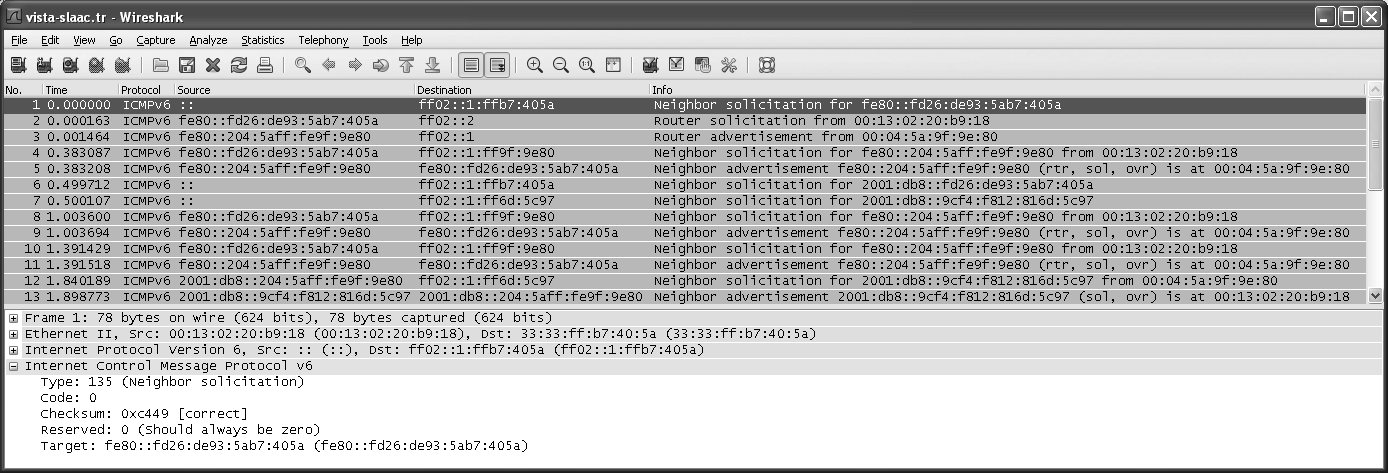
\includegraphics[scale=0.5]{imgs/6/6-23.png}
	\caption{路由器请求导致一台临近的路由器发送了一个路由器通告。请求消息被发送到所有路由器地址(ff02::2)}
\end{figure}

\begin{figure}[H]
    \centering
	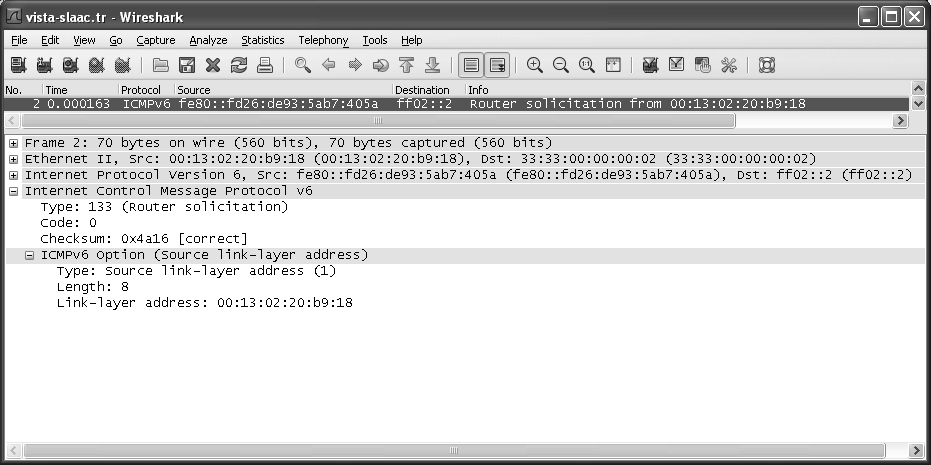
\includegraphics[scale=0.5]{imgs/6/6-24.png}
	\caption{ ICMPv6 RS消息导致一台临近的路由器提供配置信息,例如它所在网络上的全球网络前缀}
\end{figure}

\begin{figure}[H]
    \centering
	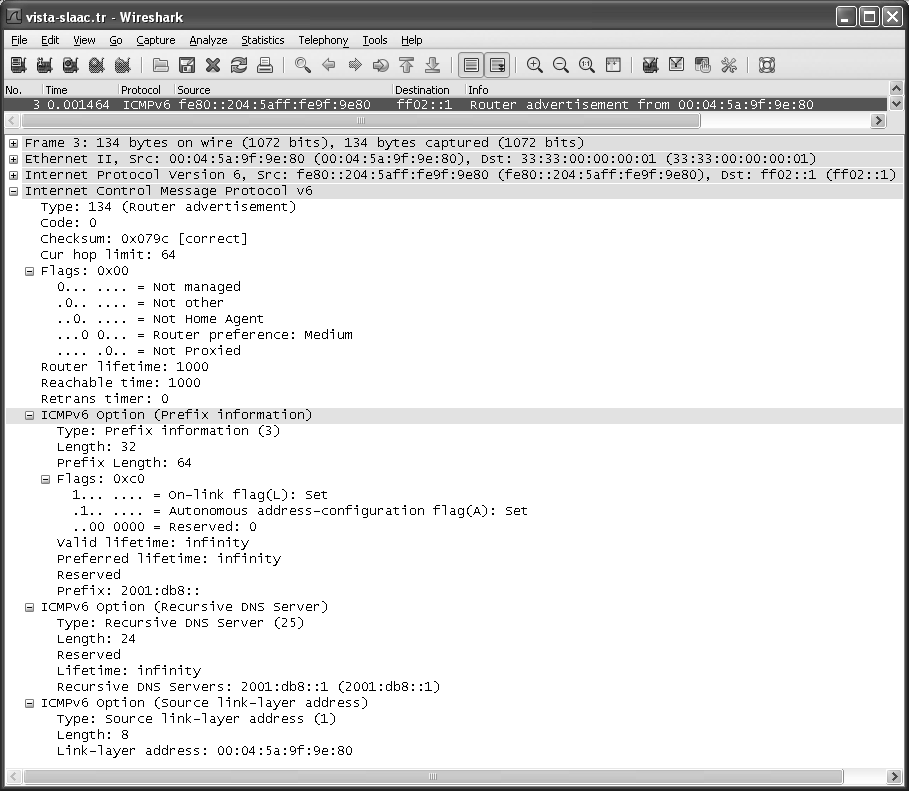
\includegraphics[scale=0.5]{imgs/6/6-25.png}
	\caption{ICMPv6 RA 消息提供了网络中的默认路由器和全局地址前缀的位置以及是否可用的信息。它
    也包括一个 DNS 服务器的位置,并表明该路由器是否可像移动 IPv6 家乡代理(本例中没有)
    那样发送通告。客户机在配置操作中可能使用部分或全部信息}
\end{figure}

\begin{figure}[H]
    \centering
	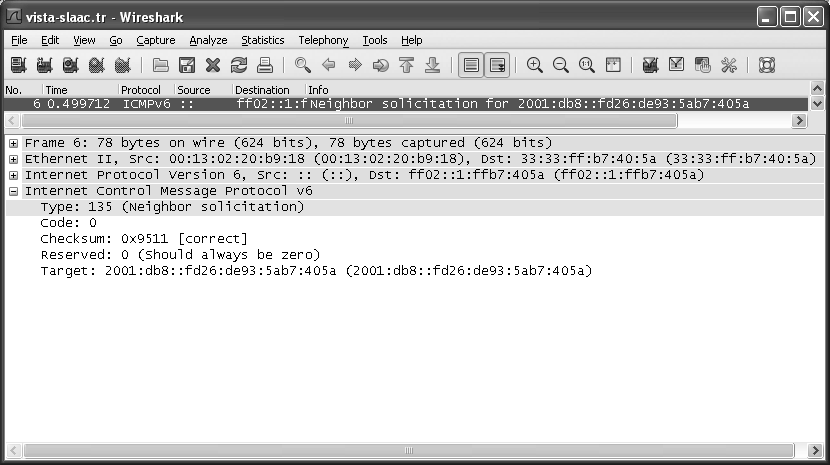
\includegraphics[scale=0.5]{imgs/6/6-26.png}
	\caption{ICMPv6 RA 消息提供了网络中的默认路由器和全局地址前缀的位置以及是否可用的信息。它
    也包括一个 DNS 服务器的位置,并表明该路由器是否可像移动 IPv6 家乡代理(本例中没有)
    那样发送通告。客户机在配置操作中可能使用部分或全部信息}
\end{figure}

\begin{figure}[H]
    \centering
	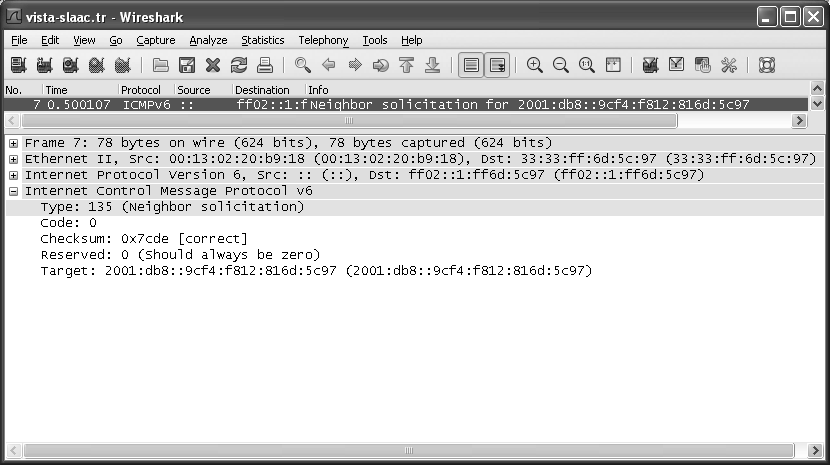
\includegraphics[scale=0.5]{imgs/6/6-27.png}
	\caption{对地址 2001:db8::9cf4:f812:816d:5c97 的 DAD}
\end{figure}

图6-27中的DAD操作针对地址 2001:db8::9cf4:f812:816d:5c97。这个地址是一个临时
IPv6地址,出于隐私保护的原因,它的低序位使用一个不同的随机数来生成。两个全球地址
之间的区别是临时地址的生命周期较短。生命周期是由以下两个值中较小的值计算得到:RA
中接收到的前缀信息选项中包含的生命周期和一对本地默认的生命周期。在 Windows Vista
的例子中,默认的有效生命周期为一星期,而默认的首选生命周期为一天。当这个消息已完
成后,客户机对自己的链路本地地址和两个全球地址执行 SLAAC。通过这些地址信息足以
进行本地或全球通信。临时地址将定期更改,以协助增强隐私保护。在不需要隐私保护的情
况下,可使用以下命令在 Windows 中禁用该功能:


\begin{verbatim}
c:l> netsh interface ipv6 Bet privacy state=disabled
\end{verbatim}

在 Linux 中,使用以下命令启用临时地址:
\begin{verbatim}
Linux# syectl -w net.ipv6.cont.al1.u8e\_tempaddr=2
Linux# sysctl -w net.ipv6.conf.default.use\_tempaddr=2
\end{verbatim}

使用以下命令禁用临时地址:
\begin{verbatim}
Linux# aysct1 -w net.ipv6.conf.a11.use\_tempaddr=0

Linux# sysctl -w net.ipv6.conf.default.use\_tempaddr=0
\end{verbatim}

\subsubsection{无状态 DHCP}
我们已提到 DHCPv6 可用于一种“无状态”模式,在这种模式下,DHCPv6服务器不
指定地址(或保留任何一台客户机的状态),但提供其他配置信息。无状态 DHCPv6定义在
\href{https://www.rfc-editor.org/rfc/rfc3736}{\href{https://www.rfc-editor.org/rfc/rfc3736}{[RFC3736]}} 中,并将SLAAC 和 DHCPv6 相结合。有人认为这种结合是一种有吸引力的部署
方案,网络管理员在部署 DHCPv4 时不必直接关心地址池。

在一个无状态 DHCPv6 部署方案中,假设节点采用DHCPv6之外的方法获得自己的地
址。因此,DHCPv6 服务器不需要处理定义在表6-1中的地址管理消息。另外,它不需要处理
建立IA 绑定所需的选项。这大大简化了服务器软件和配置工作。中继代理的操作没有改变。

无状态 DHCPv6 客户机使用 DHCPv6的 INFORMATION-REQUEST消息请求信息,该
信息由服务器发送的 REPLY 消息提供。INFORMATION-REQUEST 消息包含一个选项请求
选项,给出客户机想了解的更多信息的选项。INFORMATION-REQUEST 可能包含一个客户
机标识符选项,它允许为特定的客户机定制答案。

为了实现标准的无状态DHCPv6服务器,相应系统必须实现以下这些消息:
INFORMATION-REQUEST、REPLY、RELAY-FORW 和 RELAY-REPL。它还必须实现以下
这些选项:选项请求、状态代码、服务器标识符、客户机消息、服务器消息和接口 ID。最后
三个选项在作为中继代理时使用。作为一台可用的无状态 DHCPv6服务器,其他几个选项可
能是必要的:DNS服务器、DNS 搜索列表和可能的SIP服务器。其他可能有用但不是必需
的选项主要包括:优先级、经历的时间、用户类别、供应商类别、供应商特定信息、客户机
标识符和认证。

\subsubsection{地址自动配置的用途}
IP 地址自动配置的用途通常是有限的,这是由于路由器可能需要为同一网络中的客户机
配置特定范围的IP地址,而这台客户机自动配置的地址与该范围不一致。它在IPV4(APIPA)
环境中是好用的,这是因为专用链路本地前缀169.254/16 不能用于路由器中。因此,自己分
配IP 地址的结果是本地子网访问可能正常,但 Internet 路由和名称服务(DNS)很可能不正
常。当DNS 不正常时,大部分常见 Internet“体验”无法实现。因此,一台客户机无法获得一
个IP地址(相对容易检测),相对于获得一个实际不能有效使用的IP 地址,前者通常更有用。

\begin{tcolorbox}
    其他可能用于链路本地编址的名字服务包括Bonjour/ZeroConf (Apple)、
    LLMNR 和 NetBIOS(Microsoft)。随着时间推移,这些来自不同厂商的服务没有成
    为IETF标准,在本地环境中将名称映射到地址时的行为有很大差别。关于DNS本
    地替代者的详细信息见第11章。
\end{tcolorbox}

我们可以禁止使用 APIPA,防止系统自己分配一个 IP地址。在Windows 中,这是通过
创建以下注册表项(注册表项是一行,这里为了说明而换了行)来完成:

\begin{verbatim}
    
HKLM\SYSTEM\CurrentControlSet \Services \Tcpip\Parameters\
IPAutoconfigurationEnabled
\end{verbatim}

REG\_DWORD 值可设置为O,对所有网络接口禁用 APIPA。在Linux 中,文件/etc/
sysconfig/network 可修改为包括以下指令:

NOZEROCONE=YeS

这将禁止所有网络接口使用 APIPA。通过修改每个接口的配置文件(例如,第一个以太
网设备的 /etc/sysconfig/network-scripts/ifcfg-ethO),也可禁止特定接口使用 APIPA。

在 IPv6 SLAAC 的情况下,获得一个全局 IPv6地址相对容易,但一个名称和其地址之
间的关系并不安全,从而导致潜在的安全问题(参见第11章和第18章)。因此,在部署中暂
时仍希望避免使用SLAAC。对IPv6 全局地址禁用SLAAC 有两种方法。首先,在本地路由
器提供的路由器通告消息的前缀选项中关闭“自动”标志(配置不提供前缀选项,如前面
的例子中所示)。另外,可通过本地配置来避免客户机进行全局地址的自动配置。

在一台 Linux 客户机中禁用 SLAAC,可使用以下命令:

\begin{verbatim}    
Linux# sysct1 -w net.ipv6.conf.all.autoconf=0
\end{verbatim}

在 Mac OS或 FreeBSD 系统中禁用SLAAC(至少是针对本地链路地址),可使用以下
命令:

\begin{verbatim}
FreeBSD#

sysctl -w net.inet6.ip6.auto\_1ink1oca1=0
\end{verbatim}
而 Windows 系统中的相应禁用命令为:

\begin{verbatim}
C:\> netsh
netsh> intertace ipv6
netsh interface ipv6> get interface {ifname}managedaddress=disabled
\end{verbatim}

其中,{fname}应替换为相应接口的名称(在这个例子中是“Wireless Network
Connection”)。注意,随着时间推移,这些配置命令的行为有时会发生变化。如果这些变化
没有如预期那样执行,请查看针对当前方法的操作系统文件。

\section{DHCP 和 DNS 交互}
当一台 DHCP 客户机获得一个 IP 地址时,它接收的配置信息的重要部分是一台 DNS
服务器的IP地址。它允许客户机系统将 DNS名称转换IPv4 和/ 或IPv6地址,该地址是
进行传输层连接时协议实现所需要的。如果没有DNS服务器或其他方式将域名映射为IP
地址,大多数用户会发现他们几乎难以访问互联网系统。如果本地 DNS工作正常,它将
Internet 作为一个整体来提供地址映射,但如果配置正确,也可针对本地的专用网络(如前面
提到的.home)。

由于本地专用网络的DNS映射通常采用烦琐的手工管理,因此,将指定 DHCP地址与
相应地址的 DNS映射更新方法结合起来将会带来方便。这可通过组合DHCP/DNS 服务器或
动态 DNS(见第11章)来实现。

组合 DNS/DHCP 服务器(如 Linux dnsmasqg 包)是一个服务器程序,它可配置为提供IP
地址租约以及其他信息,也可读取一个 DHCPREOUEST 中的客户机标识符或域名,并在使
用DHCPACK 进行响应之前,通过“名称到地址”的绑定更新内部DNS 数据库。这样,由
DHCP客户机或与相同 DNS服务器交互的其他系统发起的任何后续 DNS 请求,能够在客户
机名称和新分配的IP 地址之间转换。

\section{以太网上的 PPP}

对于大多数局域网和一些广域网连接,DHCP 提供了最常用的客户机系统配置方法。
对于广域网连接(例如 DSL),常用另一种基于 PPP 的方法代替它。这种方法涉及在以太网
中携带 PPP,因此称为以太网上的 PPP(PPPoE)。PPPoE 用于广域网连接设备(例如 DSL
调制解调器)作为一个交换机或网桥而不是使用路由器的情况下。PPP 作某些ISP 建立连
接的首选,这是因为它可提供比其他配置选项(例如 DHCP)更细致的配置控制和审计日
志。为了提供Internet 连接,有些设备(例如用户PC)必须实现IP路
由和寻址功能。图6-28显示了典型的使用情况。

IsP

该图显示了一个ISP使用 DSL

为很多客户提供服务。DSL 提供一

接入集中器

条点到点的数字链路,它可与一条

点到点

以太网

家用PC

电话网络

传统的模拟电话线(称为普通老式电

话业务或POTS)同时工作。对物理

网桥

电话线的同时使用是通过频分复用

来实现的,DSL信息在比POTS更

来自电话

公司的线路

高的频率上传输。当连接到传统的

終 6-28

为客户提供使用PPPoE 的DSL服务的简化视图。

电话听筒时,需要用一个过滤器来

避免更高的DSL 频率的干扰。DSL

家用PC实现了PPPoE协议,并向ISP进行用户

调制解调器次PPP端口提供桥接服

身份认证。它也可作为家乡局域网中的路由器、

DHCP 服务器、DNS服务器或 NAT 设备

务,该端口位于ISP 的接入集中器

(AC)中,连接客户的调制解调器线和ISP的网络设备。调制解调器和 AC也支持PPPOE 协
议,在这个例子中,该用户选择将一台家用PC连接到DSL 调制解调器,并使用一个点到点
的以太网络(即仅使用一根电缆的以太网)。

在DSL 调制解调器与ISP成功建立一条低层链路后,PC可以开始进行 PPPoE交换,它

被定义在信息文档\href{https://www.rfc-editor.org/rfc/rfc2516}{\href{https://www.rfc-editor.org/rfc/rfc2516}{[RFC2516]}}中,如图6-29所示。

这个协议包括一个发现阶段和一个 PPP会话阶段。发现阶段涉及交换几个 PPPOE主动

发现(PAD)消息:PADI(初始化)、PADO(提供)、PADR(请求)和PADS(会话确认)。
在这个交换完成后,由以太网封装的一次 PPP会话开始,并最终由任何一方发送 PADT(终
止)消息来终止。如果低层连接中断,这个会话也会终止。PPPoB 消息使用图6-30所示的格
式,并封装在以太网的有效载荷区。

在图6-30中,PPPOE版本和类型字段的长度都是4位,并包含当前 PPPoE版本的值

0x1。代码字段中包含 PPPoE消息类型的提示,如图 6-30的右下部分所示。会话ID 字段包
含值0x0000表示 PADI、PADO 和PADR消息,并在后续消息中包含一个唯一的16位数字。
在PPP 会话阶段会保持相同的值。PAD 消息包含一个或多个标签,它们按 TLV 方式排列为
200

第6章

一个16位的TAG\_TYPE字段,随后是一个16位的TAG\_LENGTH 字段和一个数据可变的

标签值。表6-2给出了 TAG\_TYPE 字段的值和含义。

对等方 1

(客户机)

对等方 2

(服务器)

交换的消息

发现

PADI

(广播)

PADO

一(单播)

提供

选择

PADR

(单播)

最新网络工程师资料

www.w.gcs.cn

准备

PADS

(单播)

PPP会话

关闭

PADT

(单播)

关闭

图 6-29
PPPoE 消息交换开始于发现阶段及建立 PPP会话阶段。每个消息是一个 PAD 消息。PADI 请
求来自 PPPoE服务器的响应。PADO 提供连接。PADR 表示客户机可以从多个可能的服务器
中做出选择。PADS从选中的服务器向客户机提供一个确认。经过 PAD交换,一次PPP会话
开始。PPP会话可由任何一方发送 PADT 消息来终止,或在低层链路出现故障时关闭
将 PPPoE 的版本设置力Ox1

0

1516

31

版本

(4位)

会话 ID

(16位,发现阶段的值为0)

类型

(4位)

代码

(8位)

长度

(16位,有效载荷的长度)

图 6-30

287

288

有效载荷(可变)

[PAD 消息在有效载荷区中包含 TLV 标签]

PPPoE 以太网类型

0x8863(发现)

0x8864(PPP 会话)

代码值

0x09 (PADI)

0x07 (PADO)

0x19(PADR)

0x65(PADS)

0xA7 (PADT)

0x00(PPP 会话)

PPPoE 消息携带在以太网帧的有效载荷区。以太网类型字段在发现阶段设置为Ox8863,而设
置为 0x8864 表示携带 PPP 会话数据。对于 PAD 消息,采用TLV 方式携带配置信息,这类似
于 DHCP 选项。服务器选择一个 PPPoE 会话 ID,并在 PADS 消息中传输

表 6-2

值

0x0000

0x0101

0x0102

0x0103

0x0104

0×0105

0x0110

0x0201

0x0202

0x0203

PPPOE 的TAG\_TYPE 字段的值、名称和用途。PAD消息可能包含一个或多个标签

名称

End-of-List

Service-Name

AC-Name

Host-Uniq

AC-Cookie

Vendor-Specific

Relay-Session-ID

Service-Name-Error

AC-System-Error

Generic-Error

用途

表示没有更多标签存在。TAG\_LENGTH必须为0

包含一个UTF-8编码的服务名称(供ISP 使用)

包含一个 UTF-8编码的字符串,用于表示访问集中器

由客户机使用的二进制数据,用于匹配消息;不能被AC解释

由AC使用的二进制数据,用于防止 DoS;由客户机回显

不推荐;更多细节见\href{https://www.rfc-editor.org/rfc/rfc2516}{\href{https://www.rfc-editor.org/rfc/rfc2516}{[RFC2516]}}

中继增加该值以转发 PAD流量

请求的 Service-Name 标签不能被AC认可

AC 在执行请求的操作时出现一个错误

包含一个 UTF-8编码的字符串,用于描述一个不可恢复的错误

为了查看PPPoE的行为,我们可监控图6-28所示的一个家用系统(例如家用 PC)与一
台接人集中器之间的数据交换。图6-31显示了发现阶段和第一次 PPP会话数据包。

图6-31显示了预期的PADI、PADO、PADR 和PADS消息交换。每个消息包含一个
值为9c3a0000的Host-Uniq 标签。来自集中器的消息也包含一个值为90084090400368-
rback37.snfcca 的AC-Name 标签。图6-32显示了PADS消息的详细信息。

在图6-32中,PADS消息表示为客户机建立一次PPP会话,并使用 Oxecbd 作为会话
ID。AC-Name 标签仍然保持,表示使用原来的AC。至此,发现阶段已完成,可开始一次普
通的PPP会话(见第3章)。图6-33显示了第一次 PPP会话的数据包。

该图说明 PPPoE交换中的PPP会话阶段开始。PPP 会话开始于链路配置(PPP LCP),
这里由客户机发送一个配置请求(见第3章)。它表明客户机想使用密码认证协议(一种相对
不安全的方法)向AC认证自己。当认证交换已完成,并交换了各种链路参数(例如 MRU),
IPCP 用于获取和配置 IP 地址。注意,这时可能需要额外的配置信息(例如,ISP的 DNS服
务器的IP 地址),它取决于ISP的配置(即手工配置)。

\section{与系统配置相关的攻击}

针对系统和网络配置的攻击多种多样。从未授权客户机或未授权服务器对 DHCP 的干
扰,到耗尽资源的各种形式的DoS攻击,例如申请一台服务器可能提供的所有可能的IP地
址。这些问题很常见,这是由于地址配置基于旧的IPv4 协议,其设计出发点是假设网络可
信,而到目前为止新的协议还很少部署(安全部署就更少见)。因此,无法通过典型DHCP
部署来防御这些攻击,虽然链路层认证(例如,Wi-Fi 网络使用的WPA2)有助于限制连接
到一个特定网络的未授权客户机数量。

IETF 致力于IPv6邻居发现提供安全性,哪个邻居、什么时间或是否已部署SLAAC,
这些因素将直接影响网络运行的安全性。\href{https://www.rfc-editor.org/rfc/rfc3756}{\href{https://www.rfc-editor.org/rfc/rfc3756}{[RFC3756]}} 概括了2004年以米的信任及威胁假设,
\href{https://www.rfc-editor.org/rfc/rfc3971}{\href{https://www.rfc-editor.org/rfc/rfc3971}{[RFC3971]}}定义了安全邻居发现(SEND)协议。SEND 将 IPsec(见第18章)用于邻居发现
数据包,并结合使用加密生成的地址(CGA)\href{https://www.rfc-editor.org/rfc/rfc3972}{\href{https://www.rfc-editor.org/rfc/rfc3972}{[RFC3972]}}。这种地址由密钥散列函数而获得
所以它们只能由系统保存的适当关键信息生成。

\begin{figure}[H]
    \centering
	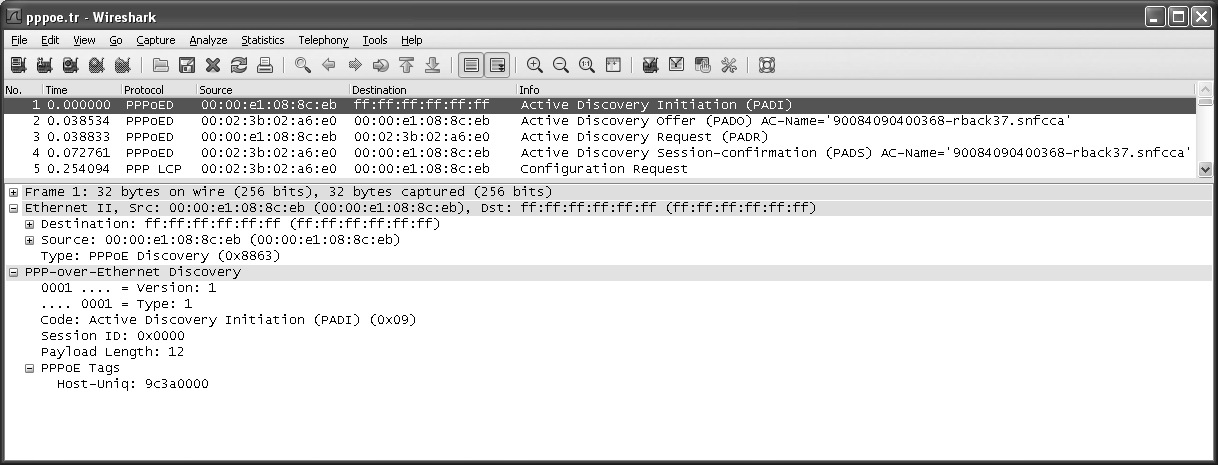
\includegraphics[scale=0.5]{imgs/6/6-31.png}
	\caption{对地址 2001:db8::9cf4:f812:816d:5c97 的 DAD}
\end{figure}

\begin{figure}[H]
    \centering
	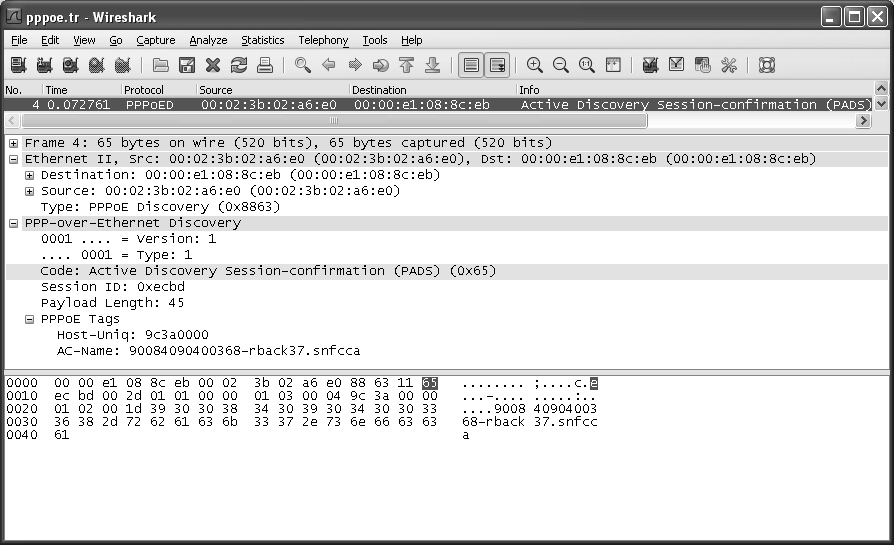
\includegraphics[scale=0.5]{imgs/6/6-32.png}
	\caption{PPPoE的PADS消息用于确认客户机和接人集中器之间的关联。这个消息
    还将会话ID设置为Oxecbd,它用于后续PPP会话数据包中}
\end{figure}

\begin{figure}[H]
    \centering
	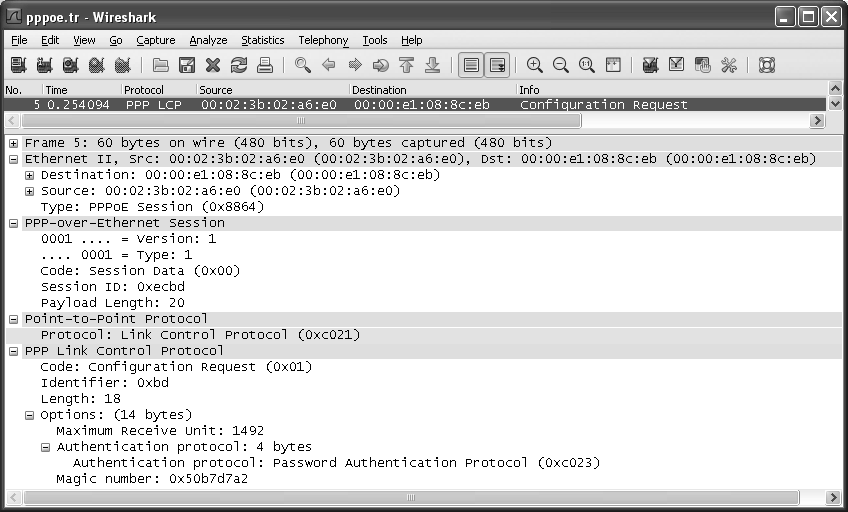
\includegraphics[scale=0.5]{imgs/6/6-33.png}
	\caption{PPPOE 会话的第一个 PPP消息是一个配置请求。以太网类型更改为Ox8864,表示这是一?
    动的PPP会话,并且会话ID 设置为Oxecbd。在这个例子中,PPP客户机使用相对不安
    密码认证协议进行身份认证}
\end{figure}

\section{总结}

主机或路由器使用 Internet 协议在 Internet 或专用网络中运行时需要一组基本的配号
路由器通常至少需要分配寻址信息,而主机需要地址、下一跳路由器和DNS服务名
位置。DHCP 可同时用于IPv4 和 IPv6,但两者之间不能直接互操作。通过DHCP,适当配
置的服务器可向请求的客户机分配一个或多个地址,并让它们租用一段时间。如果客户机想
继续使用该地址,它可更新自己的租约。客户机也可通过 DHCP 获得更多信息,例如子网掩
码、默认路由器、供应商的特定配置信息、DNS服务器、家乡代理和默认域名。当客户机和
服务器位于不同网络中,可通过中继代理使用DHCP。当使用中继代理时,一些 DHCP扩展
允许在中继代理和服务器之间携带额外信息。DHCPv6也可用于为一台路由器委托一个 IPv6
地址空间范围。

一台IPv6主机通常使用多个地址。IPv6客户机能自主生成自己的链路本地地址,这是
通过将一个特定的链路本地IPv6前缀与其他本地信息(例如从自己的MAC地址中获得的
特殊位或有助于保护隐私的随机数)相结合来实现的。要获得一个全局地址,客户机可从
ICMP 路由器通告消息或 DHCPv6服务器获得一个全球地址前缀。DHCPv6 服务器可工作在
“有状态”模式,为请求的客户机提供 IPv6地址租用;它也可工作在“无状态”模式,提供
地址之外的其他配置信息。

PPPoE 协议通过以太网携带 PPP 消息以与ISP 建立 Internet 连接,特别是那些使用DSL
提供服务的ISP。当使用PPPoE 时,用户通常有一台带以太网端口的DSL 调制解调器,该
端口就像一个网桥或交换机。PPPoE首先交换一组发现消息,以确定一个访问控制器的身份,
并建立一次 PPP会话。在发现阶段完成后,PPP流量可封装在以太网帧中,并携带不同协议
(例如IP),这可能持续到 PPPoE会话终止(不管是有意为之还是因为低层链路断开)。当使
用 PPPoE时,PPP协议配置功能,例如IPCP(在第3章中讨论),最终负责为客户机分配IP
地址。

用于IPv6无状态自动配置的DHCP 和ICMPv6 路由器通告,部署时通常没有使用安全
机制。由于这个原因,它们很容易受到一些攻击,包括未授权客户机的网络访问、生成伪造
地址的欺骗性DHCP服务器和各种形式的拒绝服务,以及客户机请求的地址超过可用地址的
资源耗尽攻击等。大多数攻击可通过为DHCP 增加安全机制来缓解,例如 DHCP 认证和最
近出现的SEND协议。但是,它们目前仍很少使用。

\section{参考文献}

[802.21-2008] 'IEEE Standard for Local and Metropolitan Area Networks—Part

21: Media Independent Handover Services,” Nov.2008.

[F07] R. Faas, "Hands On: Configuring Apple's NetBoot Service, Part 1./ Comput-

erworld, Sept. 2007.

[GC89] C. Gray and D. Cheriton, "Leases: An Efficient Fault-Tolerant Mechanism

for Distributed File Cache Consistency." Proc. ACM Symposium on Operating Sys-

tem Principles(SOSP),1989.

IARP http://www.iana.org/assignments/arp-parameters

[IBDP] http://www.iana.org/assignments/bootp-dhcp-parameters

[ID4LQ] K. Kinnear, B. Volz, M. Stapp, D. Rao, B. Joshi, N. Russell, and P. Kurapati,

“Bulk DHCPV Lease Query" Internet draft-ietf-dhc-dhcpv4-bulk-leasequery,

work in progress, Apr. 2011.

[ID4RI] B.Joshi, R. Rao, and M. Stapp, "The DHCPv4 Relay Agent Identifier Sub-

Option" Internet draft-ietf-dhc-relav-id-suboption, work in progress, June 2011.

统配置:DHCP 和自动配置

[ID6PARAM] http://www.iana.org/assignments/dhcpv6-parameters

[IDDN]G. Daley, E. Nord mark, and N. Moore, "Tentative Options for Link-

Layer Addresses in IPv6 Neighbor Discovery," Internet draft-ietf-dna-tentative

(expired), work in progress, Oct. 2009.

[IDL.2RA] B. Joshi and P. Kurapati, "Layer 2 Relay Agent Information," Internet
draft-ietf-dhc-I2ra, work in progress, Apr. 2011.

[IEPARAM] http://www.iana.org/assignments/enterprise-numbers

[MKB928233] Microsoft Knowledge Base Article 928233 at http://support

.microsoft.com

[MS-DHCPN] Microsoft Corporation, "[MS-DHCPN]: Dynamic Host Configura
tion Protocol (DHCP) Extensions for Network Access Protection (NAP)." http://
msdn.microsoft.com/en-us/library/cc227316.aspx, Oct. 2008.
\chapter{防火墙和网络地址转换}

\section{引言}

在因特网(Internet)以及协议发展的最初几年,大多数网络设计师和开发人员都来自于
大学或其他从事研究的机构。这些研究人员普遍是友好和合作的,当时的互联网系统虽然容
易遭受攻击,但并没有多少人有兴趣去攻击它。在20世纪80年代末,特别是20世纪90年
代初至中期,互联网得到了大家的普遍关注,致使人们开始感兴趣去攻陷它。成功的攻击成
了家常便饭,互联网主机在软件实现中的各种错误及未定义的协议操作造成了大量问题。因
为一些网站有大量的、各种版本的操作系统软件,对于系统管理员而言,要确保所有这些后
端系统中的各种错误均已被修复是非常困难的。此外,对于已经被淘汰的系统,要完成这项
工作几乎是不可能的。为了解决这个问题,需要一种方法来控制互联网中网络流量的流向。
今天,这项工作由防火墙来完成,它是一种能够限制所转发的流量类型的路由器。

随着部署防火墙来保护企业,另一个问题变得越来越重要:可用的IPv4 地址数量正面
临枯竭的威胁。必须采取有效的措施来管理IP地址的分配和使用。除了IPv6之外,一种
最为重要的解决机制就是网络地址转换(Network Address Translation, NAT)。采用 NAT之
后,互联网地址就不再需要是全球唯一的,因此可以在互联网的不同部分(称地址范围
(address realm))被重复使用。允许在多个范围中的同一地址重复使用,大大缓解了地址耗
尽的问题。正如我们所看到的,NAT与防火墙相结合生成的复合设备,已经演变成用于连接
终端用户的最为常见的路由器类型,包括连接家庭网络和小型企业网络至互联网的。现在,
我们将进一步探讨防火墙和 NAT 的细节。

\section{防火墙}

保证终端系统的软件是最新的和不存在任何错误需要承担巨大的管理压力,因此确保终
端系统免受攻击的焦点转为如何利用防火墙来过滤部分流量以限制流量流向终端系统。今天
防火墙很常见,并已经演化出多种不同的类型。

最为常用的两种防火墙是代理防火墙(proxy firewall) 和包过滤防火墙(packet-filter
frewall)。它们之间的主要区别是所操作的协议栈的层次及由此决定的IP 地址和端口号的使
用。包过滤防火墙是一个互联网路由器,能够丢弃符合(或者不符合)特定条件的数据包。
从 Internet 客户端的角度来看,代理防火墙则是一个多宿主的服务器主机。也就是说,它是
TCP 和UDP 传输关联的终点,通常不会在IP 协议层中路由IP数据报。

\subsection{包过滤防火墙}

包过滤防火墙作为互联网路由器,能够过滤(filter)(丢弃)一些网络流量。它们一般
都可以配置丢弃或转发数据包头中符合(或不符合)特定标准的数据包,这些标准称为过
滤器(filter)。简单的过滤器包括网络层或传输层报头中各个部分的范围比较。最流行的过
滤器包括IP 地址或者选项、ICMP报文的类型,以及根据数据包中端口号确定的各种UDP
或TCP服务。正如我们将看到的,最简单的包过滤防火墙是无状态的,而更复杂的防火墙
是有状态的。无状态的包过滤防火墙单独处理每一个数据报,而有状态的防火墙能够通过
关联已经或者即将到达的数据包来推断流或者数据报的信息,即那些属于同一个传输关联
(transport association)的数据包或构成同一个 IP 数据报(参见第10章)的IP分片。IP 分片
使得防火墙的工作变得更复杂,无状态包过滤防火墙极易被其混淆。

图7-1所示为一个典型的包过滤防火墙。在这里防火墙是一个有着三个网络接口的互联
网路由器:一个“内”接口,一个“外”接口和第三个“非军事区”(DMZ)接口。DMZ子
网能够访问外联网或DMZ,其中部署的服务器可供互联网用户访问。网络管理员会安装过
滤器或访问控制列表(Access Control Lists,ACL)(ACL 列出了什么类型的数据包需要被丟
弃或转发的基本政策)到防火墙中。通常情况下,这些过滤器将会全力拦截来自外网的恶意
流量,但不会限制从内网到外网的流量。

图7-1 一个典型的包过滤防火墙的配置。防火墙作为IP 路由器位于一个“内”网和“外”网之间,
有时是在第三个“DMZ”或外联网,只允许某些特定的流量通过。一种常见的配置是允许所
有从内网到外网的流量通过,但相反的方向只允许小部分的流量。当使用一个 DMZ时,只允
许从 Internet 访问其中的某些特定服务

\subsection{代理防火墙}

包过滤的防火墙作为一个路由器可以选择性地丢弃数据包。其他类型的防火墙,如代理
防火墙,并不是真正意义上的互联网路由器。相反,它们本质上是运行一个或多个应用层网
关(Application-Layer Gateways,ALG)的主机,该主机拥有多个网络接口,能够在应用层
中继两个连接/关联之间的特定类型的流量。它们通常不像路由器那样做IP转发,虽然现在
已经有结合了各种功能的更复杂的代理防火墙。

图7-2说明了一个代理防火墙。对于这种类型的防火墙,防火墙内的客户端通常会做特
殊配置以便关联(或者连接)到代理防火墙,而不是连接到实际提供所需服务的真正的终端
主机。(能够和代理防火墙以这种方式交互的应用需要提供相应的配置选项。)通常这些防火
墙作为多宿主主机,即便具备IP转发的能力也是被禁用的。与包过滤防火墙一样,一种常
见的配置是为“外”接口分配一个全局路由的IP 地址,“内”接口分配一个私有的IP地
址。因此,代理防火墙支持使用私有地址范围。

图7-2 代理防火墙作为一个多宿主的 Internet 主机,终止在应用层的TCP 和UDP 的连接。它不像一
个传统的IP 路由器,而更像一个 ALG。单个应用程序或代理为了其所支持的每个服务,必须
具备和代理防火墙进行通信交互的能力

虽然这种类型的防火墙是非常安全的(一些人认,这种类型的防火墙从根本上比包过
滤防火墙安全),但它是以脆性(brittleness)和缺乏灵活性代价的。特别是,因这种类型
的防火墙必须为每个传输层服务设置一个代理,任何要使用的新服务必须安装一个相应的代
理,并通过该代理来操作发起连接。此外,必须配置每个客户端以便能够找到代理(例如,
使用Web 代理自动发现协议或WPAD[XIDAD],当然也有一些替代的方法,如所请的捕捉
代理就能够处理某种类型的所有流量,而不管其目标地址如何)。至于部署方面,这些防火
墙在所有被访问的网络服务均能提前确定的环境中能工作得很好,但是添加额外的服务可能
需要网络运营者的重大干预。

代理防火墙的两种最常见的形式是 HTTP 代理防火墙(HTTP proxy firewall) \href{https://www.rfc-editor.org/rfc/rfc2616}{[RFC2616]}
和 SOCKS防火墙(SOCKS firewall)\href{https://www.rfc-editor.org/rfc/rfc1928}{[RFC1928]}。第一种类型也称为 web 代理,只能用于
HTTP 和HTTPS 协议(Web),这些协议是非常普遍的,因此这些代理会被经常使用。这些
代理对于内网用户来说就像是 Web 服务器,对于被访问的外部网站来说就像是Web 客户
端。这种代理往往也提供 Web 缓存(Web cache)功能。这些缓存保存网页的副本,以便后
续访问可以直接从缓存中获取,而不再需要访问原始的web 服务器。这样做的好处是可以
减少显示网页的延迟,提高用户访问网站的体验。一些Web 代理也经常被用作内容过滤器
(content filter),能够基于“黑名单”来阻止用户访问某些Web 网站。相反,在互联网上还
可以找到一些所谓的隧道代理服务器(tunneling proxy server)。这些服务器(例如 psiphon 和
CGIProxy)本质上执行相反的功能,以避免用户被内容过滤器封阻。

SOCKS协议比 HTTP 代理访问使用更为广泛,可用于 Web 之外的其他服务。目前正在
使用的SOCKS有两个版本:版本4和版本5。第4版为代理传输提供了基本的支持,而第
5版增加了强大的认证、UDP 传输和 IPv6 寻址。为使用SOCKS代理,应用程序在开发时必
须添加SOCKS 代理支持功能(即它必须是能够被代理的),同时通过配置应用程序能够获知
代理的位置及其版本。一旦配置完成,客户端使用SOCKS协议请求代理进行网络连接,也
可以选择性地进行 DNS查找。

\section{网络地址转换}

NAT本质上是一种允许在互联网的不同地方重复使用相同的IP地址集的机制。建立
NAT的主要动机是正在急剧减少的有限IP地址空间。使用 NAT最常见的情况是,唯一与
Internet 连接的站点仅被分配了很少的几个 IP 地址(甚至只有一个IP地址),但是内部却有
多台主机需要同时上网。当所有进出的流量均通过一个单独的NAT设备时,该设备将内部
系统的地址空间和全球互联网地址空间分割开,因此所有的内部系统可以使用本地分配的私
有IP 地址访问互联网。然而,为分配了私有地址空间的系统在互联网上提供服务是一项更
为复杂的工作。我们在7.3.4 节讨论这种情况。

NAT 的引入用以解决两个问题:IP地址枯竭和关于路由可扩展性的担忧。在刚推出的
时候(20世纪90年代初),NAT 仅作为权宜之计,是一种临时的措施,直到一些具有更大地
址数量的协议(最终是IPv6)被广泛部署止。无类域间路由(CIDR,见第2章)的发展解
决了路由可扩展性问题。NAT 是受欢迎的,因为它减少了对具备全局路由的互联网地址的需
求,同时提供了一些防火墙功能,并且仅需要很少的配置。但具有讽刺意味的是,快速发展
和广泛使用的 NAT 却严重影响了IPv6的推进进程。在IPv6 的诸多益处中,其中一项就是使
得不再需要 NAT\href{https://www.rfc-editor.org/rfc/rfc4864}{[RFC4864]}。

NAT 尽管很流行,但是存在几个缺点。最明显的是,需要做特殊配置才能使处于 NAT
内部的主机能够提供可供互联网访问的服务,因为互联网上的用户无法直接访问具备私有地
址的主机。此外,为了使NAT正常工作,每一个隶属于同一个连接或关联的双向数据包都
必须通过相同的NAT。这是因为NAT必须重写每个数据包的寻址信息,以便私有地址空间
的系统和 Internet 主机之间能够正常通信。在许多方面,NAT和互联网协议的基本宗旨是背
道而驰的:“智能边缘”(smart edge)和“哑巴中间”(dumb middle)。为完成工作,NAT 需要
跟踪每个关联(per-association)(或每个连接(per-connection))的连接状态,其操作贯穿多
个协议层,并不像传统的路由器。修改IP 层地址也需要同时修改传输层的校验码(见第10
章和第13 章关于伪头部的校验)。

NAT会对一些应用协议造成困扰,尤其是那些在应用层的有效载荷内记录IP地址信息
的协议。文件传输协议(File Transfer Protocol, FTP)\href{https://www.rfc-editor.org/rfc/rfc0959}{[RFC0959]}和 SIP\href{https://www.rfc-editor.org/rfc/rfc5411}{[RFC5411]}就是这种
类型的协议代表。它们需要一种特殊的应用层网关功能来重写应用程序的内容,以便能够毫
无修改地采用NAT或者其他的 NAT传输方法工作,这些传输方法允许应用程序自行确定如
何在NAT上工作。关于NAT的一个更完整的问题清单出现在\href{https://www.rfc-editor.org/rfc/rfc3027}{[RFC3027]}。尽管存在许多问
题,但 NAT 的使用非常广泛,并且被大多数网络路由器(基本上包括所有低端家用路由器)
所支持。今天,NAT是如此普遍,以至于应用程序设计者被鼓励开发“NAT友好”的应用
\href{https://www.rfc-editor.org/rfc/rfc3235}{[RFC3235]}。值得一提的是,尽管存在缺点,但是 NAT 所支持的基本协议(例如,电子邮件
和浏览器)被数以百万计的客户端系统在访问互联网时所采用。

NAT的工作原理就是重写通过路由器的数据包的识别信息。这种情况常发生在数据传输
的两个方向上。在这种最基本的形式中,NAT需要重写往一个方向传输的数据包的源IP地
址,重写往另一个方向传输的数据包的目的IP 地址。这允许传出的数据包的源IP 地址变为
NAT 路由器中面向 Internet 的网络接口地址,而不是原始主机的接口地址。因此,在互联网
上的主机看来,数据包是来自于具备全局路由IP 的 NAT路由器,而不是位于 NAT 内部的私
有地址的主机。

大多数的 NAT 同时执行转换(translation)和包过滤(packet fltering),包过滤的标准取
决于 NAT的动态状态。包过滤策略的选择可能会有不同的粒度,例如,NAT如何处理非请
求的数据包(它们和源自于 NAT 内部的数据包没有任何关联)取决于源和目标IP 地址和/或
源和目的端口号。处理的行为在不同的NAT上会有所不同,有时甚至在同一个 NAT上也会
随时间变化而变化。这为必须运行在 NAT后面的应用程序带来了各种挑战。

图7-3 一个将私有地址及其内部系统与互联网隔离的 NAT。私有地址的数据包不会在互联网上直接
路由,相反在进入和离开私有网络时必须通过 NAT 路由器。互联网主机看到流量来自于 NAT
的一个公共 IP 地址

\subsection{传统的 NAT:基本 NAT 和 NAPT}

很多年来都没有精确定义NAT的行为。尽管如此,根据 NAT思想行为的不同实现,已
经对出现的 NAT类型进行了分类。所谓的传统 NAT (traditional NAT)包括基本 NAT (basic
NAT)和网络地址端口转换(Network Address Port Translation,NAPT) \href{https://www.rfc-editor.org/rfc/rfc3022}{[RFC3022]}。基本
NAT 只执行IP 地址的重写。本质上就是将私有地址改写一个公共地址——往往取自于一
个由ISP提供的地址池或公有地址范围。这种类型的NAT 不是最流行的,因为它无助于减
少需要使用的IP 地址数量,全局可路由的地址数量必须大于或等于希望同时访问 Internet 的
内部主机数量。一个比较流行的做法是采用 NAPT。NAPT使用传输层标识符(即TCP和
UDP 端口,ICMP 查询标识符)来确定一个特定的数据包到底和NAT 内部的哪台私有主机关
联(见图7-4)。这使得大量的内部主机(即好几千台)能够同时访问互联网,而使用的公有
地址数量却很少,通常只需要一个。除非进行区分很重要,否则我们所说的 NAT将同时包
括传统的 NAT 和 NAPT。

图 7-4
一个基本的IPv4 NAT(左)利用地址池中的地址重写IP 地址,但是保留端口号不变。NAPT(右)
也称为IP 伪装,通常将所有的地址都重写到一个地址。NAPT 有时必须重写端口号,以避免冲
突。在这种情况下,第二个实例的端口号23479被重写为3000,以便区分返回的192.168.1.2 和
192.168.1.35 的流量

在NAT“后面”或者“内部”使用的私有地址范围不受除了本地网络管理人员之外的任
何人的限制。因此,有可能在私有范围内采用全局地址空间。原则上,这是可以接受的。然
而,当这样的全局地址也被互联网上的另一个实体所使用时,在私有范围内的本地系统极有
可能无法达到使用相同地址的公共系统,这是因为采用相同地址的本地系统会屏蔽掉使用相
同地址的远端系统。为了避免这种不良情况的发生,保留了三个 IPv4地址范围作为私有地
址范围使用[RFC1918中]:10.0.0.0/8,172.16.0.0/12,192.168.0.0/16。这些地址范围经常
被用来作为嵌人式 DHCP 服务器(见第6章)的地址池的默认值。

正如刚才所说,NAT 提供了一定程度上的类似于防火墙的安全性。默认情况下,从互联
网上无法访问 NAT私有端的所有系统。在大多数NAT 部署中,内部系统使用私有地址。因
此,必须借助NAT 的参与(根据其使用策略和行),才能保证私人地址领域和公共领域中
的主机之间的正常通信。虽然在实践中可以使用各种策略,一个共同的策略是:几乎允许所
有的传出及其返回流量(与传出流量相对应的)通过NAT,但几乎阻断所有传入的新连接请
求。此行为抑制了试图确定可利用的活动主机的IP地址“探测”攻击。此外,NAT(尤其是
NAPT)对外“隐藏”内部地址的数量和配置。一些用户认为这些拓扑信息是专有的,并应
保密。NAT 有助于这种所谓的拓扑隐藏。

正如我们所探讨的,NAT需要适合它们所支持的协议和应用程序,所以很难在隔离
NAT所处理的协议的条件下单独讨论 NAT的行为。因此,我们现在考察NAT是如何处理其
支持的每个主要传输协议的,以及如何在IPv4/IPv6 混合环境中被使用。这其中的许多行力
细节一直是 IETF 的 BEHAVE(Behavior Engineering for Hindrance Avoidance) 工作组的讨论
主题。从2007年开始,BEHAVE 已经完成了一些文件,阐明了 NAT的一致行为。这些文件
对于应用程序编写者和 NAT 开发者是非常有用的,可以了解 NAT 是如何操作的。

\subsubsection{NAT 和 TCP}

回想第1章介绍的内容,互联网中最为主要的传输层协议是TCP,使用一个IP地址和
端口号来标识一个连接的每一端。每个连接由两端组成,每个TCP连接由两个IP地址和
两个端口号唯一标识。当发起一个 TCP连接时,“主动发起者”或客户端通常发送同步包
(SYN)到“被动发起者”或服务器端。服务器端通过回复一个自己的SYN 数据包进行响应,
同时还包括一个对客户端的SYN数据包进行确认的ACK数据包。客户端回复一个 ACK数
据包给服务器端。这样,通过“三次握手”创建了连接。类似的结束(FIN)数据包被用于优
雅地关闭连接。当然,连接也能通过重置(RST)数据包来强行关闭(请参阅第13章TCP连
接的详细描述)。与TCP 相关的传统 NAT 行为要求定义在\href{https://www.rfc-editor.org/rfc/rfc5382}{[RFC5382]}中,主要涉及了 TCP
的三次握手。

以图7-3中的家庭网络为例,考察一个由地址为10.0.0.126的无线客户端发起的TCP 连
接,其目标是 Web 服务器主机www.isoc.org(IPv4地址212.110.167.157)。使用以下符号
来表示 IPv4 地址和端口号:(源IP:源端口;目标IP:目标端口),在私人段内发起连接的
数据包可表示为(10.0.0.126:9200;212.110.167.157:80)。NAT/防火墙设备作为客户端的默
认路由器,将会收到第一个数据包。NAT注意到传人的数据包是一个新的连接(因TCP
报头中的SYN标志位是打开的,见第13章)。如果策略允许(通常会,因为这是一个向外
发起的连接),数据包的源IP 地址会被修改为 NAT 路由器的外部接口的IP地址。因此,当
NAT 转发这个数据包的时候,其寻址是(63.204.134.177:9200;212.110.167.157:80)。除了
转发数据包之外,NAT还创建一个内部状态记住当前正在处理一个新连接(称NAT 会
话(NAT session))。这种状态至少包括一个由客户端的源端口号和IP地址组成的条目(称
为NAT 映射(NAT mapping))。当 Internet 服务器回复时会用到这些信息。服务器会采用客
户端初始选择使用的端口号来回复端点(63.204.134.177:9200),即 NAT的外部地址。这种
行为被称为端口保留(port preservation)。通过比对收到的数据包的目的端口号与NAT映
射条目,NAT能够确定发起请求的客户端的内部IP地址。在我们的例子中,这个地址是
10.0.0.126,所以NAT将回复的数据包从(212.110.167.157:80;63.204.134.177:9200)改
(212.110.167.157:80;10.0.0.126:9200),并对其进行转发。然后客户端收到对其请求的响应,
这样在多数情况下表示已经连接到服务器。

这个例子说明了在正常情况下是如何建立一个基本NAT会话的,但并未说明该会话是
如何被清除的。会话状态将会在交换 FIN数据包之后被删除,但并不是所有的TCP连接都
是正常关闭的。有时只是简单地将主机关闭,这样会导致应该被清除的NAT 映射仍保留在
内存中。因此当流量很少时(或者用一个 RST段表示存在其他问题),NAT 必须清除这些被
认为已经“死亡”的映射条目。

大多数的 NAT包括一个TCP连接建立的简化版本,并可以区分连接成功还是失败了。
特别地,NAT 在检测到一个传出的 SYN数据包后会激活连接计时器(connection timer),如
果回复的ACK数据包在计时器到期之前还未到达,则该会话状态将被清除。如果 ACK 数据
包到达了,计时器将被清除,并创建一个超时较长的会话计时器(session timer)(如用小时来
代替分钟)。当发生这种情况时,NAT 可能会向内部的端点发送一个额外的数据包,用于确
认该会话是否已经终止了(称为探测(probing))。如果收到ACK,NAT认识到该连接仍然
是活跃的,则重置会话计时器,并不会删除会话。如果没有收到响应(在关闭计时器(close
timer)超时之后)或者收到一个 RST数据包,表明该连接已经终止,状态将被清除。

\href{https://www.rfc-editor.org/rfc/rfc5382}{[RFC5382]}是BEHAVE 工作组的一个成果,指出一个 TCP 连接可以被配置发送“存
活”(keepalive) 数据包(见第17章),在该配置被启用时其默认的发送速率是每两个小时一
个数据包。否则,一个TCP 连接可以一直保持下去。然而,当一个连接被建立或清除时,
其最大的空闲时间是4分钟。因此,\href{https://www.rfc-editor.org/rfc/rfc5382}{[RFC5382]}要求(REQ-5)NAT 在判定所创建的连接是
否已经断开前至少需要等待2小时4分钟,而在判定部分打开或关闭的连接是否已经断开前
至少需要等待4分钟。

一个TCP NAT 面临的棘手问题是如何处理位于多个NAT 内部的主机上运行的对等
(peer-to-peer)应用\href{https://www.rfc-editor.org/rfc/rfc5128}{[RFC5128]}。一部分应用程序采用了“同时发起连接” (simultaneous open)
的技术,让连接的每一端均作为客户端同时发送 SYN数据包。TCP能够响应 SYN+ACK 的
数据包,完成连接的速度比三次握手还要快,但目前有许多 NAT并不能正确地处理这种情
况。为此,\href{https://www.rfc-editor.org/rfc/rfc5382}{[RFC5382]}要求(REQ-2)NAT处理所有有效的TCP包交换,尤其是这种连接同
时打开的情况。某些对等应用程序(如网络游戏)便采用了这种行为。此外,\href{https://www.rfc-editor.org/rfc/rfc5382}{[RFC5382]} 还
规定 NAT 将会静默丢弃那些一无所知的传人的SYN数据包。这可能会发生在同时发起一个
连接时,即当外部主机的SYN 数据包先于内部主机的SYN数据包到达 NAT 主机时。虽然这
种情况发生的可能性不大,但在出现时钟错误时确实会发生。如果传入的外部SYN数据包被
丢弃,内部的SYN 数据包还有时间来建立这个由外部的SYN数据包代表的NAT 映射。如果
在6s之内没有接收到内部的SYN数据包,NAT 可能会向外部主机发送一个错误信号。

\subsubsection{NAT 和 UDP}

针对单播 UDP的NAT 行要求定义在\href{https://www.rfc-editor.org/rfc/rfc4787}{[RFC4787]}中。NAT 在处理一系列 UDP 数据报
时所出现的问题,与处理TCP 时出现的问题大多数一样。但是UDP 有些不同,不像TCP,
它没有连接建立和清除的过程。更具体地说,它没有标识位,如用SYN、FIN 和 RST这些
位来表示一个会话的创建或销毁。此外,一个关联中的参与者也未必完全清楚。UDP 不像
TCP那样采用一个4元组来标识一个连接,相反,它是基于两个端点的地址/端口号的组
合。为了处理这些问题,如果一个绑定在“近期”没有被使用,UDP NAT会采用一个映射
计时器(mapping timer) 来清除 NAT的状态。用多大的计时器值来表示“最近”变化很大,
而\href{https://www.rfc-editor.org/rfc/rfc4787}{[RFC4787]}要求计时器至少2分钟,推荐5分钟。一个相关的问题是计时器何时刷新。
当数据包从内部传输到外部时 NAT就刷新(NAT 的对外刷新行为)或反之亦然(NAT 的对
内刷新行为)。\href{https://www.rfc-editor.org/rfc/rfc4787}{[RFC4787]}要求 NAT 保证对外的刷新行为。对内的刷新行为是可选的。

正如我们在第5章所讨论的(会在第10章再次看到),UDP 和IP 数据包可以被分片。
分片允许一个IP数据报跨越多个块(碎片),其中每个都是作为一个独立的数据报。但是,
由于UDP 是在IP 层之上,为此除了第一个分片之外,其他的分片并没有包含端口号信息,
而这是保证 NAPT正确操作所必需的信息。这同样也适用于TCP和ICMP。因此,在一般情
况下,分片并不能被NAT 或NAPT 正确处理。

\subsubsection{NAT 和其他的传输协议(DCCP,SCTP)}

尽管TCP 和UDP是迄今为止使用最广泛的互联网传输协议,但还有两种其他协议,
NAT已经为或正在为它们定义行为。数据报拥塞控制协定(Datagram Congestion Control
Protocol,DCCP)\href{https://www.rfc-editor.org/rfc/rfc4340}{[RFC4340]}提供拥塞控制的数据报服务。\href{https://www.rfc-editor.org/rfc/rfc5597}{[RFC5597]}给出了针对DCCP的
NAT 行为要求,\href{https://www.rfc-editor.org/rfc/rfc5596}{[RFC5596]}修改了DCCP 用于支持类似于TCP的同时发起连接的过程。流
控制传输协议(Stream Control Transmission Protocol,SCTP)\href{https://www.rfc-editor.org/rfc/rfc4960}{[RFC4960]} 提供了可靠的报文
处理服务,可容纳拥有多个地址的主机。[HBA09]及 [IDSNAT]给出了 NAT 与 SCTP 中应注
意的事项。

\subsubsection{NAT 和 ICMP}

ICMP 是Internet 控制报文协议,在第8章中有详细描述。它提供了关于IP数据包的状
态信息,也能够用于测量和收集网络状态信息。\href{https://www.rfc-editor.org/rfc/rfc5508}{[RFC5508]} 中定义了ICMP 的NAT 行为要
求。在ICMP 中使用NAT 时需要考虑两个问题。ICMP有两类报文:信息类的和出错类的。
出错类报文通常包含一个引起错误条件的IP 数据包(全部或部分)的副本。它们从错误被检
测到的端点,通常是在网络中,发送到数据报的原始发送方。按说,这并没有任何困难,但
是当一个ICMP错误报文通过 NAT 时,需要改写“错误数据报”的IP地址,以便它们能被
终端客户机识别(称为ICMP 的修复行动(ICMP fix-up))。信息类的报文也存在同样的问题,
但在这种情况下,大多数的报文类型是查询/响应或客户机/服务器性质的,还包括一个类
似于TCP 或UDP端口号的查询 ID (Query ID) 字段。因此,处理这些类型信息的 NAT 能够
识别向外传输的信息请求,并设置计时器用于等待响应。

\subsubsection{NAT 和隧道数据包}

在某些情况下,隧道数据包(见第3章)也需要通过NAT发送。当发生这种情况时,
NAT 不仅要修改IP 包头,还需要修改封装在其中的其他数据包的包头和有效载荷。一个这
样的例子是使用点对点隧道协议(PPTP,见第3章)的通用路由封装(GRE)包头。当GRE
包头通过NAT时,它的Call-ID 域会与NAT(或其他主机的隧道连接)冲突。如果 NAT没
能妥善处理这一映射,便不能通信。正如我们可以想象的,更多的封装层次只会使 NAT的
工作进一步复杂化。

\subsubsection{ NAT 和组播}

到目前为止,我们只讨论了 NAT的单播IP 流量。NAT 也可以被配置成支持组播流量
(见第9章),虽然这比较少见。\href{https://www.rfc-editor.org/rfc/rfc5135}{[RFC5135]} 给出了 NAT在处理组播流量时的要求。实际上,
为了支持组播流量,需要用IGMP代理来增强NAT(见\href{https://www.rfc-editor.org/rfc/rfc4605}{[RFC4605]}和第9章)。此外,从位
于NAT 内部的主机发送到外部的数据包的目的IP 地址和端口不会被修改。从内部传输到外
部的流量,其源地址和端口号可根据单播 UDP 行为修改。

\subsubsection{NAT 和 IPv6}

鉴于 NAT 在IPv4 中的广泛使用,很自然地会想到是否能够在 IPv6 中使用 NAT。目前,
这是一个有争议的问题\href{https://www.rfc-editor.org/rfc/rfc5902}{[RFC5902]}。对于许多协议设计者而言,NAT 出现了一个必要却不可
取的“缺点”—大大地增加了设计其他协议的复杂性。由于在IPv6 中没有必要节省地址
空间,而其他的NAT 特性(例如,防火墙功能,拓扑隐藏和隐私)也能通过本地网络保护
(Local Network Protection, LNP)来提供,因此人们坚决抵制在 IPv6 中使用 NAT \href{https://www.rfc-editor.org/rfc/rfc4864}{[RFC4864]}。
LNP 代表在 IPv6 中达到或者超过 NAT 性能的技术集合。

除了具备包过滤属性,NAT还支持多个地址范围共存,能够避免当站点切换ISP 时需
要改变其IP 地址的问题。例如,\href{https://www.rfc-editor.org/rfc/rfc4193}{[RFC4193]}定义了唯一的本地 IPv6 单播地址(Unique Local
IPv6 Unicast Addresses,ULA),能够为被称 NPTv6\href{https://www.rfc-editor.org/rfc/rfc6296}{[RFC6296]}的尚处于实验阶段的IPv6
到IPv6前缀转换所来用。它采用了一种算法而不是一个表格,基于前缀将一个 IPv6 地址转
换其他的(不同的)IPv6地址(例如,在不同的地址范围中),因此不需要像传统的NAT
那样需要维护单个连接的状态。此外,该算法需要修改地址以保证通用传输协议(TCP,
UDP)的“校验和”计算值保持不变。由于不需要修改网络层之上的数据包中的数据,也不
需要访问传输层的端口号,因此该方法显著地降低了 NAT的复杂性。然而,需要访问 NAT
外部地址的应用程序必须使用NAT 穿越方法或依赖于 ALG。此外,NPTv6 本身并不提供防
火墙的包过滤功能,因此必须考虑额外的部署。

\subsection{地址和端口转换行为}

NAT 的操作方式差别很大。大部分的细节涉及具体的地址和端口映射。IETF 工作组
BEHAVE 的主要目标之一是要阐明共同行为,规定哪些是最合适的。为了更好地理解所涉及
的问题,我们从一个通用的 NAT 映射例子开始(见图7-5)。

在图7-5中,我们使用符号X:表示在私有地址范围(内部主机)中的主机使用IP地址
X、端口号x(对于ICMP,采用查询ID 代替端口号)。通常 X取自于定义在\href{https://www.rfc-editor.org/rfc/rfc1918}{[RFC1918]}中的
私有IPv4地址空间。为了连接到远程地址/端口组合Y:y,NAT 需要使用一个外部地址(通
常是公共的和全局路由的)X1'和端口号x1'来创建一个映射。假设内部主机先连接到 Y1:Y1,
再连接到 Y2:y2,NAT则需先创建映射X1':x1’,再创建映射X2’:x2’。在大多数情况下,X1'
等于X2’,因为大多数网站只使用一个全局路由的IP地址。如果x1’等于x2’,映射则被认为
是重复使用的。如果x1’和x2’均与*相等,NAT 实现前面提到过的端口保留。在某些情况
下,端口保留是不可能的,所以 NAT必须处理图7-4所示的端口冲突。

图7-5 NAT地址和端口行为是由映射基于的内容刻画的。内部主机使用IP地址:端口X:x来联系
Y:y/ 和 Y2:y2。在NAT这些关联中使用的地址和端口分别是X1':x1’和X2‘:×2’。如果对于任何
Y1:y1 或者Y2:32,X1':x!'等于X2‘:x2’,则NAT 存在独立于端点的映射。若当且仅当Y1等于
12时,X1'’ I'才等于X2’:×2’,则NAT存在地址相关的映射。若当且仅当 Y1:p1 等于Y2:22时,
X1':x1'才等于X2':x2’,则NAT存在地址和端口相关的映射。若NAT的外部地址是在没有考
虑内部或者外部地址情况下选择的,则拥有多个外部地址的NAT(即其中X1'可能不等于 X2'
有一个任意地址池行为。另外还有一个选择,它可能有一个配对池行为,在这种情况下任何与
Y1 相关的关联均使用相同的X1

表7-1 和图7-5概括了由\href{https://www.rfc-editor.org/rfc/rfc4787}{[RFC4787]}定义的各种 NAT端口和地址行为。表7-1使用类
似的术语定义了在7.3.3节中介绍过的过滤行为。在所有常见的传输层协议中,包括TCP 和
UDP,所需的NAT地址和端口处理行为是独立于端点的(在ICMP中推荐使用类似行为)。
这项规定的目的是帮助应用程序确定一个确保流量能够正常工作的外部地址。我们将在7.4
节讨论 NAT穿越时加详细地讨论这些。

\iffalse
\begin{table}[htbp]
	\centering
	\caption{ NAT 的全局行为将由其转换和过滤行为定义。这些都可能是独立于主机地址、依赖于地址,或依赖于地址和端口号}
	\begin{tabularx}{\textwidth}{bss}
		% \hline
		行为名称 & 转换行沩 & 过滤行为 \\ \hline
		独立于端点的 & 对于所有的 Y2:y2,X1':x1'=X2':x2'(必需的) & 只要任何X1':x!’存在,就允许X1:x1 的任何数据包(推荐用于最大透明性) \\
		依赖于地址的 & X1':x1'=X2':x2'当且仅当Y1 =Y2 & 只要X1之前联系过Y1,就允许从 Y1:y1 到X1:x1 的数据包(推荐用于更严格的过滤) \\
		依赖于地址和端口的 & X1':x1'=X2':x2’当且仅当Y1:y1 = Y2:Y2 & 只要X1之前联系过Y1:Vl,就允许从 Y1:1 到X1:x1 的数据包 \\ \hline
    \end{tabularx}
\end{table}
\fi

如前所述,NAT 可能有几个可用的外部地址。这个地址集通常被称 NAT池(NAT
pool) 或者 NAT地址池 (NAT address pool)。多数中型到大型的 NAT 使用地址池。请注意,
NAT地址池和在第6章中讨论的 DHCP地址池不同,当然一台设备可能需要同时处理 NAT
和DHCP地址池。在这种环境中的一个问题是,当位于 NAT后的一个主机同时发起多个连
接,此时是不是为每个连接分配相同的外部IP 地址(称为地址配对 (pairing)?如果没有
限制哪个外部地址用于关联,一个 NAT的IP 地址池的行为 (IP address pooling behavior)被
认为是任意(arbitrary)的。如果它实现地址配对,它就被称为被配对(paired)。配对是所有
传输层的推荐NAT行。如果未使用配对,内部主机的通信对等端可能会错误地断定,它
正与不同的主机进行通信。对于只有一个外部地址的 NAT,这显然不成问题。

一种脆弱的NAT 类型不仅需要重载地址,也需要重载端口(称端口重載(port
overloading))。在这种情况下,多个内部主机的流量可能被修改为相同的外部IP地址和端口
号(port number)。这是一种危险的情况,因为如果多台内部主机同时访问同一台外部主机
上的服务,那么当流量从外部主机返回时便无法找到适当的目的地址。对于TCP 而言,这
是由多个外部连接共享连接标识符的4元组(源和目标地址及端口号)所导致的结果。现在
这种行为是不允许的。

一些 NAT实现了一个特殊的功能,称为端口奇偶性(port parity)。这种 NAT 尝试保持
端口号(奇数或偶数)的奇偶性。因此,如果x1 是偶数,那么x1'也是偶数,反之亦然。虽
然不如端口保留那么强大,但这样的行为有时对于使用特殊端口的特定应用协议还是非常有
用的(例如,简称为RTP 的实时协议(Real-Time Protocol),历来使用多个端口,当然也有
方法来避免出现这种问题\href{https://www.rfc-editor.org/rfc/rfc5761}{[RFC5761]})。NAT 推荐保持端口的奇偶性,但并不是必需的。随
着更复杂的 NAT 传输方法的普及,这种特性也变得越来越不重要。

\subsection{过滤行}

当 NAT为一个TCP 连接、UDP 关联或各种形式的ICMP流量创建一个绑定,不仅要创
建地址和端口映射,作为一个防火墙,还必须确定返回流量的过滤行为,这是非常常见的情
况。NAT所执行的过滤类型,尽管在逻辑上与地址和端口处理行为不同,但常常是相关的。
尤其是使用相同的术语:独立于端点,依赖于地址,依赖于地址和端口。

一个NAT 的过滤行为通常与它是否已经建立了一个地址映射相关。显然,若NAT 中缺
乏任何形式的地址映射,那么它无法转发从外到内的任何流量,这是由于它不知道需要使用
的内部目标。对于外出流量最为常见的情况,是当创建一个绑定时,相关返回流量的过滤功
能将被禁止。对独立于端点的 NAT行为,只要为内部主机创建了映射,无论来源如何,都
将允许任何传入的流量。对依赖于地址的过滤行为,仅当X1:x1 之前访问过Y1 时,才允许
Y1:y1传输流量到X1:x1。对于那些依赖于地址和端口的NAT过滤行为,仅当X1:x1 之前访
问过Y:y1时,才允许 Y1:y1 传输流量到X1:x1。最后两个之间的区别是,后面那个只是将端
口号y1考虑进去了。

\subsection{位于 NAT 之后的服务器}

采用NAT的主要问题之一,就是从外网无法直接访问位于 NAT之后的主机提供的服
务。再次考虑图7-3中的例子。如果地址为10.0.0.3的主机向互联网提供服务,如果没有
NAT 的参与便无法被访问到,至少存在如下两个原因。首先,NAT作为互联网路由器,它
必须同意转发目的地为10.0.0.3的传入流量。其次,更为重要的是,从互联网无法路由到 IP
地址 10.0.0.3,互联网中的主机也无法识别该地址。相反,NAT的外部地址被用于查找服务
器,NAT必须妥善重写和转发到达服务器的适当流量,以便它可以操作。这个过程通常称为
端口转发 (port forwarding) 或端口映射(port mapping)。

通过端口转发,进入 NAT 的流量被转发到一个位于 NAT 后面的特定配置的目的地址。
通过采用 NAT端口转发,就可以让服务器给互联网提供服务,即使它们被分配了私有的、不
可路由的地址。端口转发,通常需要采用转发到的服务器的地址和端口号来静态配置NAT。
端口转发就像一个始终存在的静态 NAT映射。如果服务器的IP地址被更改,NAT必须更新
寻址信息。端口转发也有局限性,只有一个端口号集合用于绑定每个(IP 地址,传输协议)
组合。因此,如果 NAT 只有一个外部IP 地址,它量多将相同传输协议的一个端口转发到一
个内部机器(例如,它不能支持通过TCP 80端口访问内部的两台独立的Web 服务器)。

\subsection{发夹和 NAT 环回}

当客户希望访问位于同一个 NAT私有地址空间内的服务器时,会导致一个有趣的问题。
能够支持这种场景的 NAT 需要实现发夹(hairpinning) 或者 NAT 环回(NAT loopback)。参
考图7-6,假设主机X1试图建立一个到主机X2的连接。如果X1 知道私有地址信息,X2:×2,这
没有任何问题,因为可以直接进行连接。然而,在某些情况下X1 只知道公用地址信息,X2‘:×2’。
在这些情况下,X1借助NAT采用目的地址X2':x2'尝试连接X2。当NAT意识到在 X2':x2'和
X2:x2 之间存在映射,并将数据包转发到位于NAT私有地址空间内的X2:x2 时,会触发发夹过
程。此时会出现一个问题,目的是X2:x2的数据包头部中的源地址应该是X1:x1 还是X1':x1'?

如果 NAT给X2的发夹数据包的源地址信息是X1':x!',那么这种 NAT 被称为有“外部源 IP
地址和端口”的发夹行为。这种行为是 TCP NAT
所必需的\href{https://www.rfc-editor.org/rfc/rfc5382}{[RFC5382]}。之所以需要这种行,是为了均采用全局路由地址的应用能够识别对
方。在我们的例子中,X2可能期望一个来自于X1'(例如,因为第三方系统的协调)的连接。

图7-6 一个实现了发夹或者 NAT 环回的 NAT允许一个客户机使用服务器的外部IP
地址和端口号到达位于 NAT侧的服务器。也就是说,X1能够采用地址信息
X2':×2'到达 X2:x2

\subsection{NAT 编辑}

总之,大多数IP 流量均使用 UDP和TCP 传输协议在互联网上进行传输。这些传输协
议,自己就可以很好地被NAT 支持,而无须增加额外的复杂性,这是因为它们的格式是很
好理解的。当应用层协议与它们一起携带传输层或更低层的信息,如IP 地址,NAT的问题
就会变得复杂得多。最常见的例子是FTP\href{https://www.rfc-editor.org/rfc/rfc0959}{[RFC0959]}。在正常操作中,它交换传输及网络
层的端点信息(IP 地址和端口号),所以当要传输大量数据时可以增加额外的连接。这需要
NAT 不仅改写数据报的IP 和TCP部分中的IP地址和端口号,而且也需要修改有些应用的
有效载荷本身。具有这种能力的 NAT 有时也被称次 NAT编辑器(NAT editor)。如果 NAT改
变了包的应用载荷大小,接着需要更多的工作要做。例如,TCP 为数据传输中的每个字节分
配了一个序列号(见第15章),所以如果一个数据包的大小改变了,序列号也需要相应地修
改。PPTP\href{https://www.rfc-editor.org/rfc/rfc2637}{[RFC2637]}在进行透明操作时便需要 NAT编辑器(见第3章)。

\subsection{服务提供者 NAT 和服务提供者IPV6转换}

一个相对较新的发展方向是将 NAT 从客户端移动到ISP 端。这被称为服务提供者 NAT
(service provider NAT,SPNAT)、运营商级 NAT (carrier-grade NAT, CGN),或大规模 NAT
(large-scale NAT,LSN),目的是为了进一步减轻IPv4地址枯竭的问题。采用 SPNAT,可以
想象许多ISP 的客户可以共享一个单一的全局IPv4地址。实际上,这是将汇聚点从客户这
边转移到了ISP那边。在基本形式中,常规 NAT和 SPNAT 之间没有功能上的差昇,区别只
在于推荐的使用域。然而,将 NAT功能从客户端转移到 ISP端也带来了新的安全隐患,最
终用户是否能够部署网络服务器和控制防火墙策略也成了一个问题[MBCB08]。2009年以来
的研究发现,很多用户由于使用了对等程序,因此愿意接受进来的连接[ANM09]。

SPNAT 有助于解决IPv4地址枯竭的问题,但IPv6 才是最终的解决方案。然而出于各种
已经讨论过的原因,IPv6部署已落后于预期。最初,双协议栈方案(见\href{https://www.rfc-editor.org/rfc/rfc4213}{[RFC4213]}),即每
个系统同时使用IPv6和IPv4地址,被提出用于支持向 IPv6过渡,但这种做法在IPv4地址
耗尽之前只是暂时、不那么必要的。目前正在采用更为务实的方法,就是在各种配置中结合
隧道、地址转换、双协议栈系统多种技术。在介绍完为处理现有的 NAT 而开发的方法之后,
我们将在7.6节中探讨这些。

\section{NAT 穿越}

鉴于将ALG 和NAT编辑器放置于NAT 设备中的复杂性,一种可替代的方法是应用程
序自己尝试执行 NAT 穿越(NAT traversal)。此时应用程序需要确定其流量通过NAT 时使用
的外部IP 地址和端口号,并对其协议操作做相应的修改。如果一个应用程序分布在整个网络
中(例如,有多个客户端和服务器,其中一些并不在NAT后),服务器可为位于NAT 后的客
户端之间传递(拷贝)数据,或者使这样的客户端发现对方的NAT绑定,并促成它们之间的
直接通信。使用一台服务器在客户端之间进行数据拷贝是不得已的选择,因为这其中会涉及
负载和潜在的滥用。因此,大多数时候是尝试提供一些方法,以便允许客户机之间直接通信。
直接通信的方法在对等文件共享、游戏和通信应用中已经非常广泛。然而,这种技术

往往局限于某一特定的应用程序,这意味着每一个需要NAT 穿越的新分布式应用程序,均
倾向于实现自己的方法。这可能会导致冗余和互操作性问题,最终增加了用户的挫败感和成
本。为了应付这种情况,已经建立了一个处理NAT 穿越的标准方法,它取决于几个我们在
下面的章节中讨论的不同从属协议。现在,我们先从其中一个为分布式应用所采用、健壮但
尚未成为标准的方法开始。紧接着,我们来标准化 NAT 穿越的框架。

\subsection{针孔和打孔}

如前所述,一个 NAT通常包括流量重写和过滤功能。当一个 NAT映射创建时,针对特
定应用程序的流量通常允许在 NAT 的两个方向传输。这种映射是临时的,通常只适用于在
执行时间内的单一应用程序。这类映射被称针孔(pinhole),因为它们被设计为只允许通过
一部分的临时信息流量(例如,一对IP 地址和端口号组合)。随着程序之间的通信,针孔通
常动态地创建和删除。

通过采用针孔试图使位于 NAT之后的两个或两个以上的系统直接通信的方法称为打孔
(hole punching)。\href{https://www.rfc-editor.org/rfc/rfc5128}{[RFC5128]}的3.3节描述了针对UDP 的打孔,3.4节描述针对TCP 的打孔。
为了打一个孔,一个客户机需通过一个向外的连接来访问一台已知的服务器,这样便在本地
的NAT 中创建了一个映射。当另一个客户机访问同一台服务器时,由于服务器和每个客户
机均有连接,因此知道它们的外部寻址信息。它然后在客户机之间交换它们的外部寻址信
息。一旦知道了这个信息,一个客户机便可以尝试直接连接到其他的客户机。流行的对等应
用Skype 便使用了这种方法(和其他一些方法)。

参照图 7-7,假设客户机 A 访问服务器SI,然后客户机 B也访问服务器SI。S1 会知道
A 和B的外部寻址信息:分别为IPv4 地址192.0.2.201 和 203.0.113.100。将B 的信息发送给
A(反之亦然),A可以尝试利用B 的外部地址直接联系B(反之亦然)。这是否有效取决于已
部署的NAT类型。对于连接(A,S1),其NAT状态在 N1 中,对于连接(B,S1),其NAT状
态同时在N2 和N3中。如果所有 NAT独立于端点,这些信息便足够使直接通信成为可能。
由于任何其他类型的NAT将不会接受除了S1 之外的流量,从而阻止直接通信。换句话说,
如果两台主机均位于具备依赖于地址或者同时依赖于地址和端口映射行为的NAT之后,那
么这种方法是行不通的。

图7-7
位于 NAT后的客户机上运行的应用程序可能需要一台服务器的协助,以便能够直接进行通信。
在打孔中,专门运行特定应用程序的服务器客户机之间交换信息用以建立NAT状态,如果
可能的话便可直接进行通信。当通过 NAT 时,通过使用标准的通用协议,一些应用尝试“确
定”(确定和维护)其流量将被分配的地址(和端口号)。在某些情况下这些方法将会遇到麻烦,
如在多层次的NAT环境中。在这个例子中,在S1 中客户机 A的外部可见地址是192.0.2.201,
客户机B的是203.0.113.100。然而在S2 中,客户机B的外部地址是 10.0.1.1

\subsection{单边的自地址确定}

应用程序使用一系列方法来定位其流量在通过NAT 时所采用的地址。这便称为确定
(fxing)(学习和维护)地址信息。地址确定的方法分为直接和间接两种。间接方法涉及通过
与 NAT 交换流量来推测其行为。直接方法涉及应用程序和 NAT 本身之间通过一个或者多个
特殊协议(目前还不是IETF 的标准)来进行直接会话。IETF 花费了很大的精力来发展被特
定应用程序所广泛采用的间接方法,其中为最知名的便是VoIP 应用。目前部分 NAT 也能够
支持一些直接方法。这些方法也为 NAT的基本配置做准备,因此我们将在NAT 的安装和配
置中对其进行讨论。

在没有NAT协助的情况下一个应用程序尝试确定地址,所执行的地址确定被称为是
单边类型的。这样做的应用程序被称为是执行单边的自地址确定(UNilateral Self-Address
Fixing,UNSAF)「RFC34241。顾名思义,这种方法从长远来看被认为是不可取的,但暂时
却是必要的。UNSAF会涉及一套启发式,它们并不能保证在所有情况下都能工作,特别是
因为 NAT的行为受供应商和特定环境的影响变化很大。之前提到的BEHAVE文档,其目标
就是让NAT的行为更为一致。如果被广泛采用,UNSAF 方法工作起来将更为可靠。

在大多数感兴趣的情况下,UNSAF采用类似打孔的客户机/服务器操作方式,但增加
了普适性。图7-7说明了一些在这种情况下可能出现的危害。其中一个问题就是每一台 NAT
缺乏一个单一的“外部”地址范围。在这个例子中,在客户端B和服务器SI之间有两层
NAT。这种情况可能会导致复杂性。例如,如果B上的应用希望通过一台服务器的UNSAF
获得其“外”地址,根据它是和服务器S1 通信还是和服务器S2通信,将会收到不同的回复。
最后,因为 UNSAF使用不同于 NAT 的服务器,始终存在这种可能性,即 NAT的行为报告
会随时间而改变,或者与 UNSAF 方法报告不一致。

鉴于 NAT 和UNSAF存在的各种问题,IAB——一个在IETF 中被推选出来的架构顾问
组,指出 UNSAF 协议方案必须回答针对它们规格的考虑:

\begin{itemize}
    \item 定义一个“短期”的 UNSAF方案解决有限范围问题。
    \item 定义一个退出策略/过渡计划。
    \item 讨论什么设计方案使得该方法变得“脆弱”。
    \item 确定长期、完善的技术解决方案的要求。
    \item 讨论任何知名的实际问题,或已知的经验。
\end{itemize}

这是针对协议规范规定提出的一个不寻常的列表,但它来自于不同的 NAT 和NAT 穿越
技术之间长期存在的互操作性问题。尽管存在上述问题,UNSAF 方法还是被经常使用,部
分原因是当前许多 NAT并没有一致的行为。我们现在就来看看这些方法如何使用积木的方
式来构建强大的、通用的 NAT传输技术,以最大限度地促成位于 NAT后的系统之间的通
信,甚至使跨越多个 NAT 系统之间的通信成为可能,正如图7-7所示。

\subsection{NAT 的会话穿越工具}

一个UNSAF 和 NAT穿越的主要功能,就是NAT 会话穿越工具(Session Traversal
Utilities for NAT,STUN)\href{https://www.rfc-editor.org/rfc/rfc5389}{[RFC5389]}。STUN 源自于 UDP简单隧道穿越 NAT(Simple Tunneling
of UDP through NAT),现在被称“经典的STUN”。经典STUN已经在 VoIP/SIP 应用
中使用了一段时间,但已被修改为一个可以为其他需要NAT穿越的协议使用的工具。需
要完整 NAT 穿越解决方案的应用,建议先从我们将在7.4.5节讨论(例如,ICE 和 SIP出
站)的其他机制开始。这些框架可以以一种或多种特定方式来使用STUN,被称为STUN用
法(usage)。用法可能会扩展STUN 的基本操作、报文类型,或在\href{https://www.rfc-editor.org/rfc/rfc5389}{[RFC5389]}定义的错误代
码集。

STUN是一个相对简单的客户机/服务器协议,它能够在多种环境中确定在NAT 中使用
的外部IP 地址和端口号。它也可以通过保持激活的信息来维持当前的NAT绑定。它需要在
NAT 一侧存在一台有效的“其他”合作服务器,以及几台被配置了全局IP 地址的可在互联
网上被访问到的公共STUN服务器。STUN服务器的主要工作是回显发送给它的STUN 请求,
以确定客户端的寻址信息。与一般UNSAF方法相比,该方法并非万无一失。但是STUN的
好处是它并不需要修改网络路由器、应用协议或者服务器。它仅需要客户端实现STUN 请求
协议,以及至少一台在适当位置可用的STUN服务器。STUN被设想为一种“临时”的解决
方案,直到制定和实施更复杂的直接协议,或由于IPv6 的广泛采用而使得 NAT 成为过时的
(正如目前许多在创建之后被普遍使用了10年甚至更长时间的标准协议)。

STUN 操作使用UDP、TCP 或具备传输层安全性(Transport Layer Security,TLS)的
TCP(见第18章)。STUN 用法规范定义特定用法所支持的传输协议。它次UDP和TCP使
用3478端口,为TCP/TLS使用3479端口。STUN 基础协议有两种类型的事务:请求/ 响应
事务(request/response transactions)和标志事务(indication transactions)。标志不需要响应,
并可以通过客户机或服务器生成。所有的信息包含类型、长度、值次 0x2112A442 的魔术
cookie,以及一个随机的96 位事务ID 用于匹配请求与响应或调试。每个报文始于2个0位,
并可能包含零个或多个属性(attribute)。支持特定的 STUN使用的方法(method) 在 STUN
报文类型中定义。各种STUN参数,包括方法和属性数量,均由IANA[ISP]维护。属性有
自己的类型,并可以改变长度。在一个IP数据包中,基本的STUN头通常紧挨着 UDP 传输
头,如图7-8所示。

图 7-8
STUN报文总是以2个0比特位开始,并且封装在UDP 中,当然TCP也是允许的。报文类型
字段同时给出了方法(例如,绑定)和类型(请求,响应,错误,成功)。事务ID 是一个长为
96位的数字,用于匹配请求和响应,或者在标志情况中用于调试。每个 STUN报文能够包含0
个或者多个属性,这取决于 STUN 的特定用法

基本的STUN 头的长度是20字节(见图7-8),报文长度(Message Length)字段提供了
一个最大为216-1 字节的完整的STUN报文长度(报文长度字段不包括20字节的报头长度),
由于报文总是用多个4字节来填充的,所以长度字段的低2位总是为0。通过UDPAIP 发出
的STUN报文所形成IP 数据包,若预先知道路径MTU的大小,为避免分片,其大小应小于
MTU(见第10章)。如果不知道MTU,整个数据报的长度(包括IP 和UDP 头和任何选项)
应小于576个字节(IPv4)或1280字节(IPv6)。STUN没有规定如何处理回复的报文超过
相反方向路径 MTU 的情况,所以服务器应当安排使用大小适当的报文。

通过 UDP/IP 传递的STUN报文是不可靠的,因此STUN 应用程序都需要自己来实现可
靠性。这是通过重发认丢失的报文来实现的。重传间隔是通过估计向对方发送和接受一个
报文的时间来计算的,称为往返时间(round-trip time,RTT)。在我们讨论 TCP 时(见第14
章),RTT的计算及重传计时器的设置是一个需要重点考虑的地方。STUN使用了类似的做法,
但在标准的TCP 上稍做了修改。更多细节请参考\href{https://www.rfc-editor.org/rfc/rfc5389}{[RFC5389]}。通过 TCP/IP 或带有TLS/IP 的
TCP 来传输的STUN报文的可靠性问题由TCP来处理。基于TCP 的连接可以支持多个待定
的 STUN事务。

STUN的属性被编码在一个 TLV 布局中,这也为许多其他互联网协议所采用。TLV 的
类型和长度字段均是16比特,值部分是长度可变的(最多到64KB,如果支持的话),紧随其
后的是多个4字节的填充(填充的比特可能为任意值)。在同一个 STUN报文中,属性类型
可能会出现多次,尽管只有第一个对接受者来说才是必需的。属性值低于0x8000的是必须
包含(comprehension-required)的属性,而其他的则称为可选包含(comprehension-optional)
的属性。假如一个代理收到一个拥有必须包含属性的报文但却并不知道该如何处理,就生成
一个错误。到目前为止,多数定义的属性是必须包含的[ISP]。

\href{https://www.rfc-editor.org/rfc/rfc5389}{[RFC5389]}定义了一个称之为绑定(binding)的STUN 方法,能够在请求/响应或者标
志事务中用于地址确定和保持 NAT绑定。它同时定义了11个属性,如表7-2所示。
表7-2 定义在\href{https://www.rfc-editor.org/rfc/rfc5389}{[RFC5389]} 中的STUN,有时也称为STUN2,它取代了经典 STUN。
这11个属性可能被兼容于STUN2的客户机和服务器所使用

名称

值

目的/用途

包含一个地址簇指示器和反向传输层地址(IPv4或

MAPPED-ADDRESS

0x0001

USERNAME

0x0006

MESSAGE-INTEGRITY

0x0008

ERROR-CODE

0x0009

UNKNOWN-ATTRIBUTES

0x000A

REALM

0x0014

NONCE

0x0015

XOR-MAPPED-ADDRESS

SOFTWARE

0x0020

0x8022

ALTERNATE-SERVER

0x8023

FINGERPRINT

0x8028

IPv6)

用户名称和密码,用来检验报文的完整性(达到513

字节)

在STUN 报文中的报文证书代码值(参见第18章和

\href{https://www.rfc-editor.org/rfc/rfc5389}{[RFC5389]})

包括3位差错类型、8位差错代码值和长度可变的差

错文本描述

和差错报文一起使用来表示未知属性(每个属性16

位值)

指示长期信任的证书“范围”名称

为了阻止重放攻击,在请求和应答中选择性地携带的

非重复值

MAPPED-ADDRESS 的或(XOR)版本

发送报文的软件的文本描述(例如,制造商和版本号)

提供了另一个IP地址供客户机使用,与MAPPED-
ADDRESS一起被编码

报文的CRC-32 和 0x5354554E 进行异或(XOR),如
果使用的话必须是最后的属性(可选的)

参考图7-5,地址信息为X:x的客户机总是有兴趣确定X1':x1’,即反向传输地址
(reflexive transport address) 或者映射地址(mapped address)。位于 Y1:y1 的STUN服务器将
反向传输地址包含在一个STUN 报文的 MAPPED-ADDRESS 属性中,并将其回复给客户机。
MAPPED-ADDRESS 属性包含一个8位的地址族(Address Family) 字段,一个16位的端口
号(Port Number)学段,以及一个32位或128位的地址(Address)字段,这取决于地址族
字段(IPv40x01,IPv6为0x02)指定是IPv4还是IPv6。之所以包含这个属性是为了与
经典的STUN保持向后兼容。更重要的属性是 XOR-MAPPED-ADDRESS 属性,其中包含与
MAPPED-ADDRESS 完全相同的属性值,但需要与魔术 cookie 值(对于IPv4)或事务 ID与
魔术的cookie串联值(对于IPv6)异或。以这种方式使用异或值的原因是为了检测并绕过通
用ALG,防止它们查看和改写通过的任何IP地址。这种ALG 是很脆弱的,因为它们可能
改写像 STUN这样的协议所必需的信息。经验表明,在数据包负载中异或IP地址足以绕过
ALG。

一个 STUN 客户机,包括多数的VoIP 设备和软件电话应用如 pisua[PJSUA],初始时
均需要配置一个或者多个 STUN服务器的IP 地址或者名称。之所以希望使用 STUN服务
器是因为当该应用程序最终与对方对话时它能看到相同的IP 地址,尽管要确定可能有点困
难。通常使用布局在互联网中的STUN服务器(例如,stun.ekiga.net, stun.xten.com, numb.
viagenie.ca)便足够了。一些服务器能够通过DNS服务(SRV)记录来发现(参见第11章)。
图 7-9所示的就是一个 STUN 绑定请求的例子。

\begin{figure}[H]
    \centering
	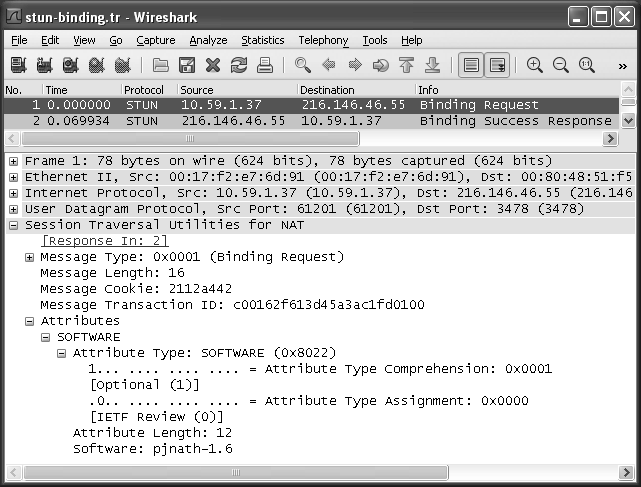
\includegraphics[scale=0.7]{imgs/7/7-9.png}
	\caption{一个 STUN绑定请求。该请求包含一个96位的事务ID 和一个用于识别发起请求的客户机的SOFTWARE 属性。属性包含了10个字符,但是其值向上舍人为4的倍数,给出的属性值是12。报文长度16 包含了用于包含属性类型和长度的4个字节(并未包含STUN头部)}
\end{figure}

图7-9所示的STUN 绑定请求例子由客户机先初始化。事务ID 是随机选择的,其请
求将被发送到 numb.viagenie.ca (IPv4 地址216.146.46.55 和216.146.46.59),这既是一台
STUN 服务器,也是一台 TURN服务器(参见7.4.4节)。请求中包含了用于识别客户应用的
SOFTWARE 属性。在这种情况下,请求由 pinath-1.6 初始化。这是包含在 pisua 中的 “PJSIP
NAT 助手”应用。信息长度包含用于属性类型和长度的4字节,加上用于保持属性的12个
字节。pjnath-1.6的长度只有10字节,但是属性长度总是向上取整为接近4字节的倍数。在
穿越过一个 NAT 之后,所得的应答如图7-10所示。

\begin{figure}[H]
    \centering
	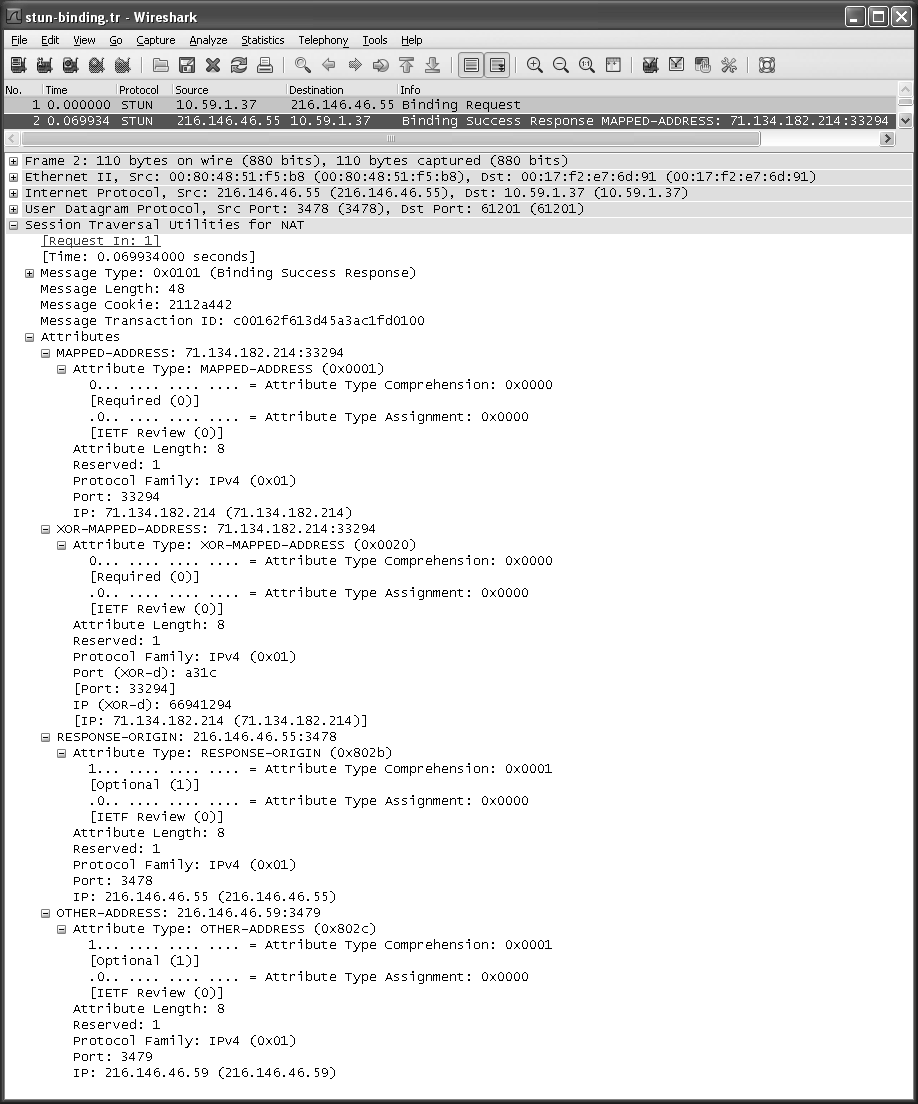
\includegraphics[scale=0.5]{imgs/7/7-10.png}
	\caption{包含4个属性的 STUN绑定回复。MAPPED-ADDRESS 和 XOR-MAPPED-ADDRESS 属性含服务器反向寻址信息。其他的属性用于实验性质的 NAT 行为发现机制\href{https://www.rfc-editor.org/rfc/rfc5780}{[RFC5780]}}
\end{figure}

图7-10所示的绑定回复以编码为属性集合的方式为客户机提供了有用的信息
MAPPED-ADDRESS 和 XOR-MAPPED-ADDRESS 属性表明,STUN服务器确定了服务
器反向地址71.134.182.214:33294。RESPONSE-ORGIN 和 OTHER-ADDRESS 属性被实系
设施用于发现NAT行为\href{https://www.rfc-editor.org/rfc/rfc5780}{[RFC5780]}。第一个属性给出了用来发送STUN报文的通信终端
(216.146.46.55:3478,与发送 IPv4地址和UDP端口号相匹配)。第二个属性表示假如客户村
请求“更改地址”或“改变端口”的行为,哪个IPv4源地址和端口号(216.146.45.59:3479
将被使用。后者的属性相当于现在已经过时的经典 STUN 中的 CHANGED-ADDRESS 属性。
如果一个请求要求变更地址或端口,如果可能,回复给客户机的协作 STUN服务器应该尝试
使用一个不同的地址。

STUN 可用于执行地址确定之外的其他一些称为机制(mechanisms) 的功能,包括 DNS
发现、重定向到备用服务器的方法和报文完整性交换。机制是在一个特定的STUN 用法的上
下文中选择的,所以一般被认是可选的STUN功能。一个更重要的机制是提供身份和报文
完整性验证。它有两种形式:短期信任机制(short-term credential mechanism) 和长期信任机
制(long-term credential mechanism)。

短期信任持续一个会话;特定时间由 STUN用法来定义。长期信任支持多个会话;它们
对应一个登录ID 或账户。短期信任通常用于特定的信息交换,长期信任在分配某些特定资
源时才使用(例如和TURN一起,见7.4.4节)。在能够被截获的地方,从来不用明文来发送
密码。

短期信任机制使用 USERNAME 和 MESSAGE-INTEGRITY这两个属性。两者在任何请
求中都是必需的。USERNAME 属性暗示需要哪种凭证,允许信息的发送方使用合适的共享
密码来形成一个报文的完整性校验(基于报文内容计算一个MAC值,见第18章)。使用短
期信任时,假定某种形式的凭证信息(例如,用户名和密码)在前期已经被交换过。用于形
成 STUN信息完整性校验的凭证被编码在 MESSAGE-INTEGRITY属性中。能够形成一个有
效的 MESSAGE-INTEGRIT属性值,意味着发送方当前持有的凭证是正确和最新的。

长期信任机制通过一种称为摘要挑战(digest challenge)的方法来保证凭证是最新的。
使用这个机制,客户端在初始化请求时不需要提供任何认证信息。服务器会先拒绝请求,但
在响应中会包含一个 REALM 属性。这可以被客户端用来确定需要提供何种凭证才能通过验
证,当然客户端可能有各种服务的凭据(例如,多个 VoIP 账户)。和 REALM一起,服务器
会提供一个永不重用的NONCE值,客户端能够用它来形成后续的请求。这种机制还采用了
MESSAGE-INTEGRITY属性,但其完整性功能是通过包含NONCE值来计算的。因此,偷
听了之前长期信任交换的窃贼很难回复一个有效的请求(因NONCE 值是不同的)。如何在
凭证中使用 NONCE及相关问题在第18 章有详细讨论。长期信任机制无法用来保护 STUN
标志,因为这些事务不是以请求/响应对来操作的。

\subsection{利用 NAT 中继的穿越}

利用 NAT 中继的穿越(Traversal Using Relays around NAT,TURN) \href{https://www.rfc-editor.org/rfc/rfc5766}{[RFC5766]}为两个
或多个系统提供了一种通信方式,即使它们均位于并未协作的NAT后。作为支持在这种情
况下通信的最后手段,它需要一个中继服务器在无法通信的系统之间传递数据。使用STUN
和一些 TURN特定报文的扩展,即使大多数其他方法都失败了它也能照样支持通信,只要每
个客户端均能连接到不在 NAT后的公共服务器。如果所有的NAT 均与 BEHAVE 标准兼容,
TURN 就没有必要存在了。直接通信的方法(即不使用TURN)总是优于采用TURN服务器
的方法。

根据图 7-11,通常位于 NAT后的TURN 客户机会访问位于公共互联网上的TURN服
务器,并暗示了它希望连接的其他系统(称对等(peer))。通过使用一种特殊的 DNS
NAPTR记录(见第11章和\href{https://www.rfc-editor.org/rfc/rfc5928}{[RFC5928]}),或通过手动配置,便可以找到用于通信的服务器的
地址和相应的协议。客户端从服务器端获得的地址和端口信息,称为中继传输地址(relayed
transport address),就是TURN 服务器用于和其他对等客户机通信的地址和端口号。客户端
也获得了它自己的服务器反向传输地址。对等客户机也得到了代表它们外部地址的服务器反
向传输地址。这些地址是客户端和服务器用来连接客户机及其对等所必需的。交换寻址信息
的方法并没有在TURN 中定义。相反,为了能够更加有效地使用TURN服务器,这些信息
必须使用其他一些机制来完成交换(例如,7.4.5节的ICE)。

图 7-11
根据\href{https://www.rfc-editor.org/rfc/rfc5766}{[RFC5766]},一个 TURN服务器通过中继来帮助位于“坏”(bad) NAT 之后的客户机之
间通信。客户端和服务器之间的流量可采用 TCP、UDP 或使用了TLS的TCP。服务器和一个
或多个对等客户机之间的流量使用UDP。中继是通信的最后手段,直接的方法才是首选

客户端使用 TURN 命令来创建和维护服务器上的分配(allocation)。一个分配类似于
一个多路NAT绑定,包括(唯一)中继传输地址,每个对等客户机需要使用它到达本机。
通过UDP/IPv4使用传统的TURN报文来发送服务器/对等数据。通过增强也能支持TCP
\href{https://www.rfc-editor.org/rfc/rfc6062}{[RFC6062]}和IPv6(IPv4和IPv6之间的中继)\href{https://www.rfc-editor.org/rfc/rfc6156}{[RFC6156]}。封装的客户/服务器数据内包括
发送信息或者接受相关数据的相应的对等客户机的信息。客户/服务器连接已被指定为使用
UDP/IPV4、TCP/IPv4 和来用TLS的TCPAIPv4。建立一个分配要求验证客户端的身份,通常
使用 STUN 长期信任机制。

TURN 支持两种客户端和对等之间拷贝数据的方法。第一种使用STUN方法来编码数
据,称为发送(Send)和数据(Data),定义在\href{https://www.rfc-editor.org/rfc/rfc5766}{[RFC5766]}中,这是 STUN 指示器 (indicator),
因此无须认证。其他的方法采用特定于 TURN 的概念,称为隧道(channel)。隧道是客户端
和对等之间的通信路径,相对于发送和数据方法负载较轻。通过隧道传递的报文使用一个较
小的、4个字节的报头,与TURN使用的较大的STUN格式报文是不兼容的。一个分配最多
可以拥有16K个隧道。发展隧道方法,有助于减小一些数据包比较小的应用的延迟和开销,
如VolP等。

在操作中,客户端使用一个 TURN定义的 STUN 分配(Allocate)方法来发出一个获取
分配的请求。如果成功,服务器响应一个成功指示器和已经分配的中继传输地址。如果客户
未能提供足够的验证信息,服务器可能会拒绝请求。现在,客户端必须发送更新的报文以保
持分配活跃。如果客户机10分钟内不发送信息,那么分配就到期,除非客户机在分配请求
中包含了一个用于指定不同生命周期值的 STUN LIFETIME 属性。通过请求一个生命周期
0的分配,就能将其删除。分配到期时,与其相关的所有隧道便也到期了。

分配通常使用“5元组”表示。在客户端,5元组包括客户端的主机地址和端口号、服
务器传输地址和端口号以及用于与服务器通信的传输协议。除了客户端的主机传输地址和端
口被替换服务器的反向地址和端口之外,服务器端使用了相同的五元组。一个分配可能有
零个或多个相关联的权限(permission),以限制允许通过TURN服务器的连接模式。每个权
限包括一个 IP 地址的限制,只有当源地址匹配的数据包到达TURN服务器,其数据有效载
荷才会被转发到相应的客户端。如果不能在5分钟内刷新,权限将被删除。

TURN通过6种方法、9个属性以及6个错误响应代码增强STUN。这些大致可以分为支
持建立和维护分配、认证以及操作隧道。6种方法和它们的方法号如下:分配(Allocate)(3),
刷新(Refresh)(4),发送(Send)(6),数据(Data)(7),创建权限(CreatePermission)(8),
隧道绑定(ChanneIBind)(9)。前两种方法用于建立并保持分配存活。Send和 Data 使用 STUN
报文封装从客户端发送到服务器的数据,反之亦然。GreatePermission 用于创建或刷新一个权
限,ChannelBind通过一个16位的隧道号与一个特定的对等客户端相关联。错误报文表明与
TURN 功能相关的问题,如认证失败或资源耗尽(例如,隧道数)。表7-3给出了由 TURN定
义的9个 STUN 属性名称、值以及目的。

表7-3

由 TURN 定义的 STUN属性

名称

CHANNEL-NUMBER

LIFETIME

XOR-PEER-ADDRESS

DATA

XO R-R ELAYED-ADDRESS

值

0x000C

Ox00OD

0x0012

0x0013

0x0016

EVEN-PORT

0x0018

REQUESTED-TRANSPORT

0x0019

DONT-FRAGMENT

0x001A

RESERVATION-TOKEN

0x0022

目的/用处

表示和数据关联的信道

请求分配超时(秒)

一个对等的地址和端口号,采用异或(XOR)编码

为一个发送或者数据指示保存数据

为一个客户机分配的服务器地址和端口

中继的传输层地址信息使用一个偶数端口的请求,
择性地按顺序请求分配下一个端口

一个客户机用来请求采用一个特定的传输层来形成传
输层地址,值来自于 IPv4 协议或者IPv6 下一跳头部字
段值

请求设置发送到对等数据包中的IPv4 头部中的“不分
片”位

服务器保存的一个中继传输层地址的唯一标志,这个
值作为一个引用提供给客户端

\begin{figure}[H]
    \centering
	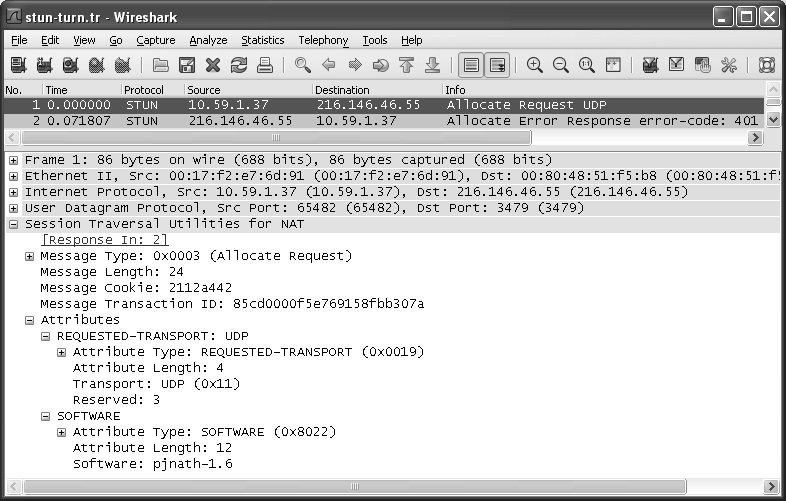
\includegraphics[scale=0.5]{imgs/7/7-12.png}
	\caption{TURN 分配请求是一个使用报文类型0x0003的STUN 报文。这一请求还包括 REQUE TRANSPORT 和SOFTWARE 属性。但是并未包含认证信息。根据STUN的长期信任,这个请求将失败}
\end{figure}

TURN 请求采用了STUN报文的形式,其中报文类型是一个分配请求。图7-12给出了
一个例子。根据STUN 的长期信任机制,图7-12所示的初始分配请求没有包括认证信息,
因此会被服务器拒绝。如图 7-13所示的一个分配错误响应表示服务器拒绝了请求。

\begin{figure}[H]
    \centering
	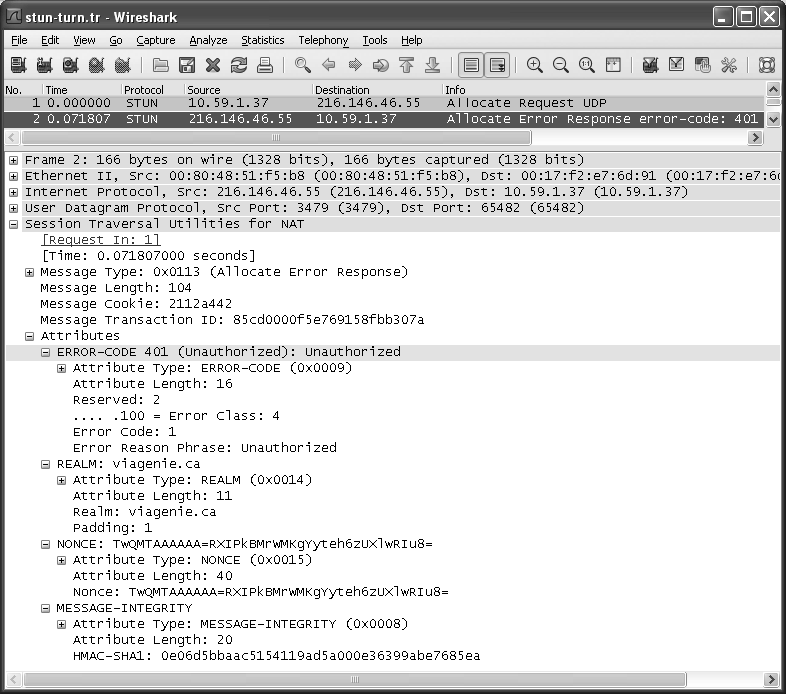
\includegraphics[scale=0.5]{imgs/7/7-13.png}
	\caption{TURN分配错误响应包含属性值为401的ERROR ̄CODE属性(未授权)。该报文是受完整性保护的,并包含了客户端为形成下一个认证分配请求所必需的REALM和NONCE属性}
\end{figure}

图7-13中的错误信息提供了 REALM属性(viagenie.ca)和客户端需要形成它下一个
请求的NONCE值。报文还包括了 MESSAGE-INTEGRITY 属性,所以客户端可以检查该
报文没有被修改,请求中属性 REALM 和 NONCE 是正确的。随后的请求中包含的属性有
USERNAME、NONCE 和 MESSAGE-INTEGRITY。参见图 7-14;

\begin{figure}[H]
    \centering
	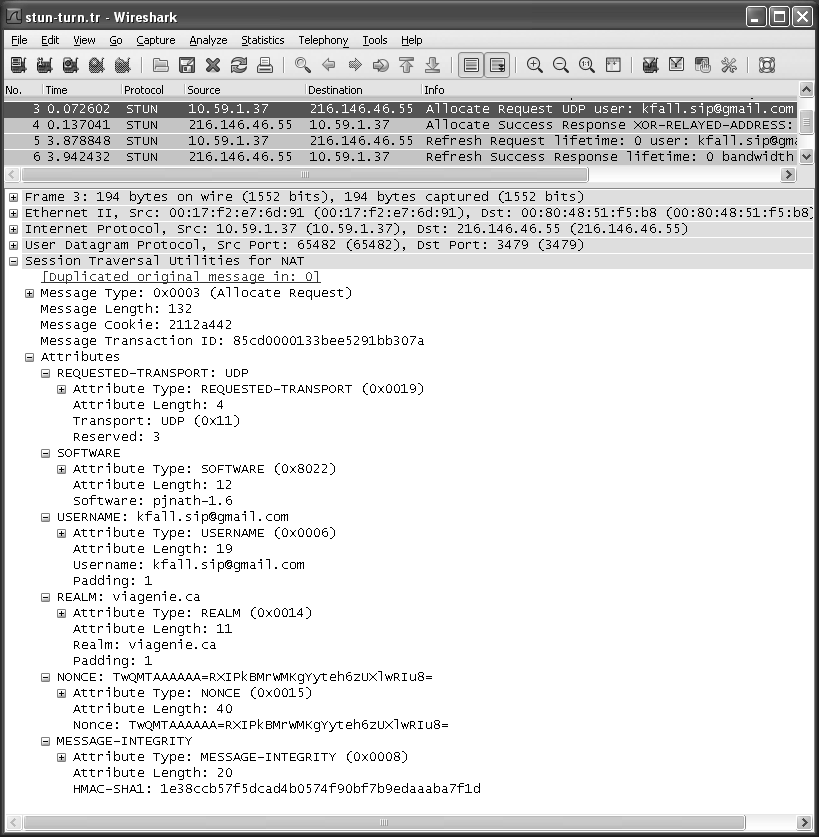
\includegraphics[scale=0.5]{imgs/7/7-14.png}
	\caption{第二个 TURN 分配请求包括了 USERNAME、REALM、NONCE 和 MESSAGE-INTEGRITY 属性。使用这些服务器能够验证报文的完整性及客户端的身份。如果成功,服务器将验证请求并分配}
\end{figure}

如图7-14所示,在收到包含长期信任的请求之后,服务器计算自己版本的报文完整性
值,并与MESSAGE-INTEGRITY属性值进行比较。如果它们匹配,TURN服务器便有足
够的信息确定客户端持有正确的密码。然后,它允许分配并指示将结果返回给客户端(见
图7-15)。

如图7-15所示,分配请求是成功的,中继传输地址是216.146.46.55:49261(注意,
Wireshark 执行 XOR操作来显示解码后的地址)。此时,客户端可以继续使用TURN服务器
来中继和对等客户端之间的通信。一旦这个完成后,分配可以被删除。大概4s后,图7-15
所示的包5和6表明客户端请求删除分配。这个请求作为一个刷新,其生命周期设为0。服
务器响应一个表示成功的指示器,并清除分配。请注意,BANDWIDTH 属性已包含在分配
和刷新成功指示器中。此属性定义在\href{https://www.rfc-editor.org/rfc/rfc5766}{[RFC5766]} 初稿中,但最终被弃用,本来打算用于保存
在分配中允许的峰值带宽,单位是KB/s。在未来可能会重新定义该属性。

\begin{figure}[H]
    \centering
	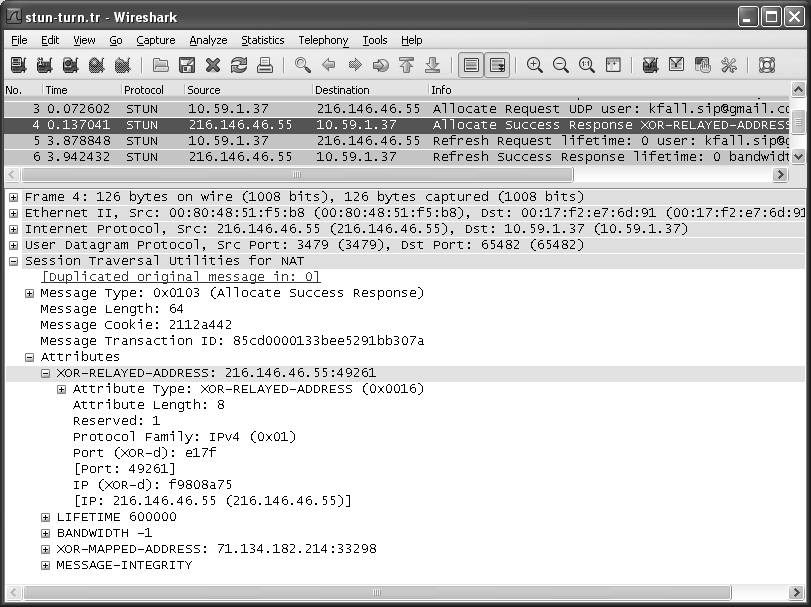
\includegraphics[scale=0.5]{imgs/7/7-15.png}
	\caption{一个 TURN 分配成功响应。报文是受到完整性保护的,包括了用于确定由 TURN服务器分配的端口和地址的XOR-RELAYED-ADDRESS 属性。如果不刷新的话,分配将被删除}
\end{figure}

正如前面提到的,TURN存在的缺点是流量必须通过TURN服务器进行中继,这可能
会导致低效的路由(即TURN服务器可能会离客户端和最优的对等客户端距离较远)。此外,
其他某些从对等到客户端的流量内容并不会通过TURN服务器。这包括ICMP值(见第8
章)、TTL(跳数限制)字段值和IP DS 字段(DS feld)值。此外,请求 TURN 的客户端必须
实现 STUN 长期信任机制,并有由TURN服务器操作员分配的登录凭证或账户。这有助于
避免不加控制地使用开放TURN 服务器,但也增加了配置的复杂度。

\subsection{交互连接建立}

鉴于 NAT的广泛部署及各种为穿越它们所必须采用的机制,一种称交互式连接建立
(Interactive Connectivity Establishment,ICE)\href{https://www.rfc-editor.org/rfc/rfc5245}{[RFC5245]}的通用功能被发展出来,用于帮助
位于NAT后的UDP 应用程序主机建立连接。ICE是一套启发式,利用它应用程序能够以
一个相对可预见的方式来执行 UNSAF。在它的操作中,ICE使用了其他协议,如TURN和
STUN。有一种方法可以扩展ICE 使其支持基于TCP 的应用[IDTI]。

ICE 使用并扩展了“请求/应答”协议,如单播SIP连接建立时的会话描述协议(SDP)
\href{https://www.rfc-editor.org/rfc/rfc3264}{[RFC3264]}。这些协议会提供一项拥有一组服务参数的服务,还包括一组选定的选项。找到
ICE 客户并纳入使用SDP/SIP 建立通信的VoIP 应用已经变得越来越普遍。然而在这种情况
下,ICE 被用于建立媒体流(如使用 RTP\href{https://www.rfc-editor.org/rfc/rfc3550}{[RFC3550]}或 SRTP\href{https://www.rfc-editor.org/rfc/rfc3711}{[RFC3711]}通话中的音频或视
频部分)的NAT 穿越,而另一种称为SIP 出站(SIP outbound)的机制\href{https://www.rfc-editor.org/rfc/rfc5626}{[RFC5626]}用于处理
SIP 信令,如谁是被叫方。尽管在实际中,ICE 主要用于基于 SIP/SDP 的应用,它也可以作
为一个通用的NAT 穿越机制用于其他应用程序。这样的一个例子就是将ICE定义为可扩展
的报文和现场协议(Extensible Messaging and Presence Protocol, XMPP) \href{https://www.rfc-editor.org/rfc/rfc6120}{[RFC6120]} 核心的
一个扩展,并与Jingle 一起使用[XEP-0176]。

通常,ICE用于创建两个 SDP实体(称代理(agent))的通信,首先需要确定一组
每个代理都能够用来与其他代理进行通信的候选传输地址(candidate transport address)。参
照图 7-11,这些地址可能是主机传输地址、服务器反向地址或中继地址。ICE 可同时使用
STUN 和TURN 来确定候选的传输地址。接着,ICE 根据优先分配算法对这些地址进行排序。
相比于那些需要中继的地址,该算法为能够提供直接连接的地址分配更大的优先级。然后,
ICE 为对等代理提供优先的地址集合,其中对等代理也会有类似的行。最终,两个代理商
量好一套最好的可用地址,并将选择的结果告知对方。使用一系列编码为STUN报文的检查
(check)可用于确定哪些候选的传输层地址是可用的。ICE 通过几项优化可以减少同意选定
候选地址的延迟,但这超出了本文的讨论范围。

ICE 开始试图发现所有可用的候选地址。这些地址可能是本地分配的传输层地址(如果
是多宿主代理便有多个主机)、服务器反向地址,或由TURN 确定的中继地址。在为每个地
址分配一个优先级后,每个代理使用SDP将优先级列表发送给对等方。对等代理执行相同
的操作,这导致每个代理会有两个优先名单。然后每个代理通过连接2个列表形成一个完全
相同的优先候选对(candidate pair) 集合。采用特定的顺序在候选对中执行一系列的检查可
以确定最终采用哪些地址。一般情况下,优先排序更加倾向于具有较少 NAT或者中继的候
选对。一个由ICE 指派的控制代理(controlling agent)将确定最终选择的候选对。控制代理
根据其优先顺序指定(nominate)使用哪个有效的候选对。控制代理可能会尝试所有对,并
随后做出选择(称常规选择(regular nomination)),或者可能使用第一个可行的对(称积
极选择 (aggressive nomination))。通过一个用于指定特定对的STUN 报文中的标志来表示常
规选择,而通过在每个请求中设置选择标志来表示积极选择。

利用被检查的地址信息在两个代理中交换 STUN 绑定请求信息,就是发送检查。检查是
由计时器触发,或者受来自于对等代理连接的调度(称触发检查(triggered check))。通过
包含地址信息的STUN绑定回复表示响应。在某些情况下这可能会揭示一个新的用于代理的
服务器反向地址(例如,当STUN 或者 TURN服务器最初确定候选地址后,代理之间又使用
了一个新的不同于以往的NAT)。如果发生这样的情况,代理获得了一个称为对等反向候选
(peer-refexive candidate)的新地址,该地址将被ICE 添加到候选地址中。ICE 检查是通过使
用基于 STUN 短期信任机制的完整性检查及 STUN 的 FINGERPRINT属性来完成的。当采
用TURN 时,ICE 客户机用TURN权限来限制针对感兴趣的远端候选地址的TURN 绑定。

ICE 采用了不同的实现概念。Lite 实现是专为没有采用 NAT 的系统部署所设计的。它们
永远不会充当控制代理,除非与另一个 Lite 实现进行交互。它们也不会执行前面提到的完全
(full)实现所做的检查。发出的STUN 报文会表明ICE实现的类型。所有ICE实现必须遵守
STUN\href{https://www.rfc-editor.org/rfc/rfc5389}{[RFC5389]},但 Lite 实现将永远只能充当STUN服务器。ICE通过表7-4中所述的属性
扩展 STUN。

名称

'PRIORITY

USE-CANDIDATE

表7-4 由ICE 定义的 STUN 属性

值

0x0024

0×0025

目的/ 用处

计算出相关候选地址的优先级

通过控制代理来指示选择候选地址

防火樯和网络地址转换

235

(续)

名称

ICE-CONTROLLED

ICE-CONTROLLING

值

0×8029

0x802A

目的丿用处

指示报文的发送者就是被控制的代理

指示报文的发送者就是控制代理

检查是一个包含PRIORITY属性的STUN绑定请求。该值等于由4.1.2节描述的算法
所指定的值\href{https://www.rfc-editor.org/rfc/rfc5245}{[RFC5245]}。当发送方是正在控制或者被控制的代理时,STUN 请求中会分别包
含 ICE-CONTROLLING 和 ICE-CONTROLLED 属性。一个控制代理可能还包括一个 USE-
CANDIDATE 属性。如果存在,这种属性指示控制代理在后续使用中想要选择的代理。

\section{配置包过滤防火墙和 NAT}

NAT 通常只需很少的配置(除非端口转发正在使用),但是防火墙通常需要进行配置,
有时它们需要大量的配置。大多数家庭网络中,同一台设备需要同时提供NAT、IP 路由和
防火墙等功能,并可能需要一些配置。虽然每个配置在逻辑上是独立的,但是配置文件、命
令行界面、网页控件或其他网络管理工具有时会合并。

\subsection{防火墙规则}

包过滤防火墙,必须给予一套说明匹配条件的指令来选择丢弃或者转发流量。现在配
置一个路由器,网络管理员通常配置一个或多个 ACL。每个 ACL 包含一个规则列表,其中
每个规则通常包含模式匹配条件(pattern-matching criteria)及其对应的动作(action)。匹配
条件通常允许规则表达网络层或传输层中的包字段值(例如,源和目的地IP 地址、端口号、
ICMP 类型字段等)以及方向(direction)的说明。方向模式采用基于方向的方式来匹配流量,
允许不同的规则集分别应用于传入与传出的流量。许多防火墙还允许在处理顺序中的某一点
应用防火墙规则。这方面的例子包括能够在IP 路由决策过程之前或之后指定一个ACL。在
某些情况下(尤其是当使用多个接口时),这种灵活性就变得很重要。

当一个包到达时,在适当的ACL 中按照顺序匹配其中的匹配条件。对于大多数的防火
墻而言,按照第一个匹配的规则采取动作。典型动作包括阻止或加速符合某项规则的流量,
还可以调整计数器或写一个日志条目。一些防火墙可能也包括附加功能,如将特定的数据包
发往应用程序或其他主机。每个防火墙厂商通常有自己的方法来指定规则,其中思科系统的
ACL 格式已成为许多企业级路由器厂商所广泛支持的一种格式。家庭用户的ACL 配置通常
使用一个简单的Web 界面。

一个非常流行的用于构建防火墙的系统是包含在现代版本 Linux 中的iptables,它是使
用一个称为 NetFilter[NFWEB] 的网络过滤功能来构建的。这是早先称为 ipchains 功能的演
变,iptables 能够提供无状态和有状态包过滤以及 NAT 和 NAPT 的支持。我们应研究它是如
何工作的,以更好地理解防火墙以及现代 NAT 提供的各种功能。

iptables 包含过滤表格(table)和过滤链(chain)的概念。一个表格包括许多预定义
的链,也可能包含0个或者多个用户自定义的链。三个预先定义的表格为:filter,nat 和
mangle。默认的 filter 表格用来处理基本的包过滤,包括了预先定义的 INPUT、FORWARD
和OUTPUT三条链。这些动作分别对应于目的地是防火墙路由器本身运行程序的流量、路
由时通过防火墙的流量以及从该防火墙主机发出的流量。nat 表格包含了 PREROUTING、
OUTPUT 和 POSTROUTING三条链。mangle 表格有五条链,主要用于任意修改数据包。

每条过滤链是一个规则列表,每条规则包含匹配条件及其对应的动作。这个动作(也
称为目标(target))可能是执行一条用户自定义的链或者执行如下预定义的动作:ACCEPT
DROP,QUEUE 和 RETURN。当一个数据包匹配上述之一的规则时,便立即采取响应的动
作。ACCEPT (DROP)是指数据包将被转发(丢弃)。QUEUE 是指数据包将被提交给一个用
户程序处理,RETURN 是指处理将在之前触发的一条链中继续,形成了一种包过滤链子调用。

一个完整的防火墙配置设计是非常复杂的,而且针对用户特定需求和它们所需要的服
务类型,因此我们不会在此尝试穷举每一个。相反,下面的例子只是给出了 iptables 中一小
部分可能的用法。下面的例子给出了一个 Linux 防火墙配置文件。它是由一个 shell触发的,
如 bash:

\begin{verbatim}
    
EXTIF="exto"

INTIF="etho"

LOOPBACK INTERFACE="10"

ALL="0.0.0.0/0"

# matches al1

# set default filter table policies to drop

iptables -P INPUT DROP

iptables -P OUTPUT DROP

iptables -P FORWARD DROP

# all local traffic OK

iptables -A INPUT -1 SLOOPBACK\_INTERFACE -j ACCEPT

iptables -A OUTPUT -i SLOOPBACK\_INTERFACE -j ACCEPT

# accept incoming DHCP requests on internal interface

iptables -A INPUT -i $INTIF -p udp -s 0.0.0.0\

--sport 67 -d 255.255.255.255 --dport 68 -j ACCEPT

# drop unusual/suspect rCP traffic with no flags set

iptables -A INPUT -P tcP --tcP-flags ALL NONE -j DROP
\end{verbatim}

这个例子说明了用户在设置一个过滤规则列表时的灵活性。初始时,所有的链都采用
默认规则(-P选项),将会影响所有没有匹配上规则的数据包。通过设置 filter 表中的 INPUT
和OUTPUT 链,所有进出本计算机(采用伪接口(pseudo interface)1o 表示)的流量都被设
置ACCEPT(即接受)。其中,j选项意味着“跳转”到一个特定的处理目标。接下来,
从IPv4地址0.0.0.0进来的UDP广播流量,以及目的地采用DHCP 端口号(67,68)的本
地/子网广播流量,都经由内部接口被允许通过。接着,将所有进来的TCP 段(参见第13
章)的标志(Flags)字段和1(ALL)相与(AND),再将结果与0(NONE)比较。当所有的
标志字段都为0时匹配成功,说明这不是一个非常有用的TCP段(正常情况下,第一个 TCP
段包含SYN标志位,其后的每个 TCP 段将包含一个有效的ACK 标志位)。

尽管这个例子所阐明的语法是针对 iptables 的,但是它的功能却不是。多数过滤性防火
墙都能够执行类似的检查和动作。

\subsection{NAT 规则}

在多数简单的路由器中,NAT能够配置为和防火墙一起工作。在基本的Windows 系统
中,NAT 被称互联网连接共享(Internet Connection Sharing,ICS),在 Linux 中被称为IP
伪装(IP masquerading)。以 Windows XP 为例,ICS有一些独有的特征。它为运行ICS 的主
机分配了 192.168.0.1 的“内部”IPv4地址,同时启动了一个 DHCP服务器和 DNS服务器。
其他的主机地址从 192.168.0/24子网段中分配,并将ICS主机作为DNS服务器。因此,在
已经有其他的主机或者路由器提供了上述服务或者存在地址冲突的网络中,ICS 不应该被启
用。通过修改注册配置能够修改默认的地址范围。

在 Windows XP 中为一个互联网连接启动ICS可以通过网络设置向导来完成,或者在一
个已经运行了的互联网连接中改变“高级”属性(在“配置|网络连接”中)。至此,用户可
能决定允许别的用户来控制或者关闭共享网络连接。这个功能也被称互联网网关设备发现
和控制(Internet Gateway Device Discovery and Control,IGDDC),它采用了通用的即插即用
的框架,允许在一个客户机中控制本地互联网网关,该内容在7.5.3 节中有介绍。所支持的
功能包括连接、断开,同时读取各种状态信息。与ICS一起工作的Windows 防火墙功能支
持创建服务定义(service definition)。服务定义等同于之前定义的端口转发。为了使之有效,
需要选中互联网连接中的“高级”属性标签,再添加一个新的服务(或者编辑一个现有的服
务)。然后,用户在外部接口和内部服务器中便能够填入合适的TCP 和UDP端口号。这样
也为进来的连接提供了一种配置 NAPT的方法。

和Windows一样,Linux 也将伪装功能和防火墙实现结合在一起。下面的脚本以一种简
单的方式来配置伪装。注意这种脚本是用来说明的,并不建议在产品中推荐使用。

\begin{verbatim}
    
EXTIF="ext0"

echo "Default FORWARD policy: DROP"

iptables -P

FORWARD DROP

echo

"Enabling NAT

on $EXTIF for hosts 192.168.0.0/24"

iptables -t nat -A POSTROUTING -O $EXTIF -s 192.168.0.0/24\

-j MASQUERADE

echo "FORWARD policy: DROP unknown traffic"

iptables

-A INPUT -i SEXTIF -m state

--state NEW, INVALID -j DROP

iptables -A FORWARD -i $EXTIF -m state --state NEW, INVALID -j DROP
\end{verbatim}

此处,filter 表格中FORWARDING链的默认策略被设置为DROP。在路由已经决定采
取哪个合适的外部接口时,下一个项目是对从192.168.0.0/24子网中获取了IPv4 地址的主机
流量的地址进行重写(通过NAT 中的nat表格和-t nat选项来实现)。由于NAT 的有状态的
工作方式,目前将有可能调整filter表格的规则以只允许为 NAT所知的连接的流量通过。最
后的两行调整了 INPUT和 FORWARD链,将丢弃任何无效或者未知(NEW)的传入流量。
特的操作符 NEW 和 INVALID 是在 iptables 命令之内定义的。

\subsection{与 NAT 和防火墙的直接交互:UPnP、NAT-PMP 和 PCP}

在多数情况下,一个客户系统希望或者需要和防火墙直接交互。例如,一个防火墙需要
为不同的服务配置或者再配置,以保证针对特定端口的网络流量不会被丢弃(创建一个“小
孔”)。在一个代理防火墙正在被使用的情况下,每个客户机必须被告知代理的身份。否则的
话,就无法越过防火墙进行通信。目前已经开发了许多支持客户机和防火墙之间进行通信的
协议。其中两个最为流行的是通用即插即用(Universal Plug and Play,UPnP)和 NAT端口
映射协议(NAT Port Mapping Protocol, NAT-PMP)。UPnP 这个标准是由一个称为 UPnP论
坛的工业组开发的。NAT-PMP 目前是IETF 中一个到期的草稿文件。NAT-PMP 为绝大多数
的Mac OS 系统所支持。UPnP 在 Windows 系统中是原生支持的,也能够被添加到 Mac OS
和 Linux 系统。UPnP 也被数字生活网络联盟(DLNA)[DLNA]用于家庭网络中支持消费电
子设备发现协议。

通过采用UPnP,被控制的设备通过第一个 DHCP来配置IP 地址,如果 DHCP 不可用
的话,就采用动态链接-本地地址配置(参见第6章)。接着,简单服务发现协议(Simple
Service Discovery Protocol, SSDP) [XIDS] 向控制点(例如,客户机)宣布设备的存在,
同时允许控制点来查询设备的其他信息。SSDP 使用了基于UDP 的两个 HTTP变种来代
替更为标准的TCP,它们被称为HTTPU 和 HTTPMU[XIDMU],其中后者使用组播寻址
(IPv4 地址239.255.255.250,端口 1900)。如果使用基于IPv6的SSDP,那么将采用如下
的地址:ffO1:C(本地节点),ff02:(本地连接),ff05:c(本地站点),ff08:c(本地组织),
ffOe::c(全局)。

后续的控制和事件通知(eventing)是由通用事件通知架构(General Event Notification
Architecture,GENA)控制的,它采用了简单对象访问协议(Simple Object Access Protocol,
SOAP)。SOAP支持客户/服务器远程过程调用(Remote Procedure Call,RPC)机制,使
用编码在可扩展标记语言(eXtensible Markup Language,XML)中的报文(XML 通常用于
Web 网页中)。UPnP 被消费电子设备所广泛采用,包含音频和视频回放和存储设备。NAT
和防火墙设备是采用互联网网关设备(Internet Gateway Device,IGD)协议控制的[IGD]。
IGD 支持一些别的功能,包括学习 NAT 映射和配置端口转发的能力。感兴趣的读者可以从
MiniUPnP 项目主页[UPNPC]中得到一个简单的IGD 客户端用于实验。UPnP IGD 的第二个
版本[IGD2]增加了对IPv6的支持。

UPnP是一个包含 NAT 控制及其他不相关规范的广泛架构,而NAT-PMP 是另外一种方
法,它针对与NAT设备进行程序通信。NAT-PMP 是苹果公司用于零配置网络的服务器搜索
协议 Bonjour 规范的一部分。NAT-PMP 并没有采用发现过程,这是由于被管理的设备通常
就是可通过DHCP获取的默认网关。NAT-PMP 使用UDP端口 5351。NAT-PMP 支持一个用
于学习 NAT外部地址和配置端口映射的请求/响应协议。它也支持一个基本的事件机制,当
NAT外部地址发生改变时能够通知监听者。这是在外部地址发生改变时通过采用一个 UDP
组播报文发送到地址 224.0.0.1(即所有主机的地址)来完成的。NAT-PMP 使用UDP端口号
5350用于客户机/服务器的交互,5351端口用于组播事件通知。根据端口控制协议(Port
Control Protocol, PCP) [IDPCP]的建议,NAT-PMP 的概念可被扩展用于支持 SPNAT。

\section{IPv4/IPV6 共存和过渡中的 NAT}

随着最后一个顶层单播IPv4地址在2011年早期被分配出去,向IPv6的过渡便开
始加速了。曾经认为通过为主机配备双栈功能(例如,实现完整的IPv4 和 IPv6协议栈)
\href{https://www.rfc-editor.org/rfc/rfc4213}{[RFC4213]},网络服务就会过渡到只有IPv6 的操作。目前认为IPv4 和 IPv6将会共存更长一
段时间,甚至可能是无限期的,这是由于各种经济原因网络基础设施可能会使用IPv4 或者
IPv6或者两者同时使用。假设这是真的,那就需要支持IPv4 和 IPv6系统之间的通信,无论
它们是否拥有双协议栈。目前用于支持IPv4和IPv6组合的两种主要方法是隧道和转换。隧
道方法包括Teredo(见第10章)、双协议栈精简版(DS-Lite)和 IPv6快速部署(6rd)。虽然
DS-Lite 采用SPNAT作为其架构的一部分,但在\href{https://www.rfc-editor.org/rfc/rfc6144}{[RFC6144]}描述的框架中给出了一种更单一
的转换方法,它使用了我们在第2章中见到过的嵌入了IPv4的IPv6地址。我们将在本节了
为详尽地讨论 DS-Lite 和转换架构的细节。

\subsection{双协议栈精简版}

DS-Lite(Dual Stack Lite,双协议栈精简版)\href{https://www.rfc-editor.org/rfc/rfc6333}{[RFC6333]}是一种希望在内部运行IPv6的
服务提供者更容易过渡到IPv6(同时支持传统的IPv4用户)的方法。从本质上讲,它可以
让供应商把重点放在部署一个可操作的IPv6核心网上,还通过使用少数的IPv4地址为客
户提供了IPv4 和IPv6连接。该方法结合了在IPv6 中的IPv4 (IPv4-in-IPv6)的“软电线”
(softwire) 隧道与 SPNAT\href{https://www.rfc-editor.org/rfc/rfc5571}{[RFC5571]}。图7-16显示了这种部署的设想。

图7-16
DS-Lite 通过使用一个只有IPv6的架构使服务提供者能够支持IPv4和IPv6 客户网络。通过
在服务提供者边缘使用 SPNAT,能够最大限度地减少IPv4 的使用

在图7-16中,每个客户网络运行IPv4 和IPv6的任意组合。假定仅使用IPv6 来管理服
务提供者的网络。客户对IPv6互联网的访问是通过采用传统的IPv6路由来完成的。对于
IPv4 的访问,每个客户使用一个特殊的“前”网关(在图7-16中标记为“B4”)。一个B4
设备提供了基本的IPv4服务(如DHCP服务,DNS代理等),但也以多点到点的隧道方式封
装了客户的IPv4流量,并在“后”设备(图7-16中标记为“AFTR”)处终止。这个 AFTR
设备为目标是IPv4互联网的流量执行了解封操作,并为相反方向的流量执行封装操作。
AFTR还执行了 NAT,并作为一种形式的SPNAT。更具体地说,AFTR 可以利用客户隧道终
端的标志信息来消除从 IPv4 互联网返回到 AFTR的流量的二义性。这将允许多个客户使用
相同的IPv4地址空间。通过利用 DHCPv6中的一个 AFTR-Name 选项\href{https://www.rfc-editor.org/rfc/rfc6334}{[RFC6334]},一个 B4
设备能够学习到它所对应的 AFTR设备的名称。

回忆一下第6章中对IPv6快速部署(6rd)的讨论是非常有益的。鉴于 DS-Lite 通过一
个服务提供者的IPv6网络为客户提供了到IPv4 的访问,6rd 的目标是通过一个服务提供者
的IPv4 网络为客户提供到 IPv6的访问。本质上,它们使用类似的框架组件,但却来取了相
反的做法。然而,6rd 中从IPv6地址映射到相应的IPv4 隧道端点(反之亦然)的计算,是通
过一个无状态的地址映射算法完成的。框架中也使用了无状态地址转换,用于IPv4 和 IPV6
之间的全协议转换,这是我们接下来需要讨论的。

\subsection{使用 NAT 和 ALG 的 IPv4/IPV6 转换}

采用隧道技术解决IPv4 和IPv6共存问题的最大缺点是,采用一种地址类型的主机上
的网络服务无法被采用了另一种地址类型的主机直接访问。由此,一个只有IPv6 的主机就
只能够与其他支持 IPv6 的系统进行通信。这种状况是不能接受的,因为只支持IPv6 的新系
统将无法访问在传统的IPv4互联网上提供的服务。为了解决这个问题,在2008年至2010
年间花了很大的努力开发了一个能够直接在IPv4 和IPv6间进行转换的框架。借鉴 NAT-
PT\href{https://www.rfc-editor.org/rfc/rfc2766}{[RFC2766]}已有的糟糕经验,这个框架被认为太脆弱了,针对今后不断变化的使用也没有
可扩展性,因此最终被舍弃了\href{https://www.rfc-editor.org/rfc/rfc4966}{[RFC4966]}。

IPv4 和IPv6转换的框架在\href{https://www.rfc-editor.org/rfc/rfc6144}{[RFC6144]}中有描述。这个基本的转换架构同时采用了有状
态的和无状态的方法来完成IPv4 和IPv6地址之间的转换、DNS 的转换(参见第11章),以
及在任何必要情况下(包括ICMP 和FTP)添加的行或者ALG 的定义。本节我们将讨论的
内容包括基于\href{https://www.rfc-editor.org/rfc/rfc6145}{[RFC6145]}和\href{https://www.rfc-editor.org/rfc/rfc6146}{[RFC6146]}的有状态和无状态的IP地址转换,以及第2章中讨
论过的源于\href{https://www.rfc-editor.org/rfc/rfc6052}{[RFC6052]}的寻址。其他针对特定协议的转换问题将在后续的章节中讨论。

\subsubsection{已转换的IPv4 地址和可转换的IPv4地址}

在第2章,我们已经讨论了内嵌有IPv4的IPv6地址结构。这样的地址是IPV6地
址,但是将其作为一个函数的输入,则能够输出一个对应的IPv4地址。这个函数也能轻
易地被反转。内嵌IPv4的IPv6地址存在两种重要的类型,称已转换的IPv4地址(IPv4-
converted address) 和可转换的IPv4地址(IPv4-translatable address)。每个提到的地址类型
是其他类型的一个子集。也就是说,如果我们将每个地址类型看作一个集合,那么会有(可
转换的IPv4)C(已转换的IPv4)C(内嵌的IPv4)C(IPv6)。可转换的IPv4地址是能够
通过有状态的方式来确定一个 IPv4 地址的IPv6地址(参见7.6.2.2节)。

IPv4 和IPv6地址之间的算法转换涉及使用第2章中讨论过的前缀。这个前缀可能是
一个知名前缀(WKP) 64:ff9b::/96 或者另外一个为服务提供者所有并和转换器一起使用的
特定于网络的前缀。WKP 只用于表示常规的全局可路由的IPv4地址,不能表示私有地址
\href{https://www.rfc-editor.org/rfc/rfc1918}{[RFC1918]}。此外,WKP也不能用于创建可转换的IPv4地址。这样的地址应该在服务提供
者网络内部被定义,因此不适合在一个全局范围中使用。

WKP 是很有趣的,因为相对于 Internet 校验和,它是校验和中立(checksum-neutral)
的。回想一下第5章介绍的 Internet 校验和的计算方法。假如我们将前缀64:ff9b::/96看作
是十六进制值0064,ff9b,0000,0000,0000,0000, 0000,0000组成的,这些值的和是 ffff,它
的补码正好是0。因此,当一个 IPv4 地址包含 WKP 前缀时,包中作为转换结果(例如,在
IPV4 头部中的 TCP或者 UDP 校验和)的相关 Internet 校验和是不会受影响的。自然地,恰
当选择的特定于网络的前缀也能是校验和中立的。

在接下来的两个小节中,我们将使用符号To4(A6,P)来表示从前缀为P的IPv6地
址A中得到的IPv4地址。P可以是WKP 或者是某个特定于网络的前缀。我们将使用符号
To6(A4,P)来表示从前缀为P的IPv4地址A中得到的IPv6地址。注意,除了一些特殊的
情况之外,A6 = To6(To4(A6,P),P) 和 A4 = To4(To6(A4,P),P)。

\subsubsection{无状态转换}

无状态的 IP/ICMP 转换(Stateless IP/ICMP Translation,SIIT)是指不采用状态表格进行
IPv4 和IPv6数据包转换的方法\href{https://www.rfc-editor.org/rfc/rfc6145}{[RFC6145]}。转换中无须查找表格,只需要使用一个可转换
的IPv4地址及一个预定义的用于转换IP头部的计划。大部分情况下,IPv4选项是不需要转
换的(被忽略),IPv6扩展头部也不需要转换(分片头部例外)。唯一的例外是未到期的IPv4
源路由选项。如果存在这种选项,数据包将被丢弃,并产生相应的ICMP 差错报文(目的不
可达,源路由失败,见第8章)。表7-5描述了当转换一个 IPv4报文到IPv6 时,IPv6 头部
字段是如何赋值的。

IPv6 字段

表7-5 当从IPv4转换到IPv6 时创建一个IPv6 头部的方法

分配方法

版本(Version)

DS 字段 /ECN (DS Field/ECN)

流标志(Flow Label)

负載长度(Payload Length)

下一个头部 (Next Header)

跳数限制 (Hop Limit)

源 IP 地址 (Source IP Address)

目的IP 地址(Destination IP Address)

设置 6

拷贝自 IPv4 头部中的相同值

设置为0

设置为IPv4 的总长度减去 IPv4 头部长度(包含选项)

设置IPv4 协议字段(或者58,如果协议字段值为1)

设置为44来表示是一个分片头部,如果创建的IPv6 数据报是一个

分片或者 DF位没有被设置

设置为IPv4 TTL 字段减去1(如果这个值为0,则该报文将被丢弃,

同时产生一个ICMP超时报文,参见第8章)

设置6(IPV4源IP 地址,P)

设置次6(IPv4 目的IP地址,P)

在转换的过程中,IPv4 头部被抽离,取而代之的是IPv6头部。假如到达的IPv4 数据报
相对于下一个链路的 MTU来说太大了,并且其头部中的DF 位也未设置,那么将会产生多
个IPv6 分片数据包,其中每个将包含一个分片头部。当到达的IPv4数据报是一个分片时,
也会发生这种情况。\href{https://www.rfc-editor.org/rfc/rfc6145}{[RFC6145]}建议当到达的IPv4数据报头部的DF 位值0时,不管转换
器是否需要执行分片,也不管达到的数据报是否是一个分片,都需要在结果 IPv6 数据报中
包含一个分片头部。这将允许IPv6接收者知道IPv4的发送者并没有采用PMTUD。当包含
了一个分片头部时,需要根据表7-6所列的方法来设置字段值。

分片头部字段

下一个头部 (Next Header)

分片偏移(Fragment Offset)

更多分片位(More Fragments Bit)

标识(Identification)

表7-6从IPv4 到IPV6转换时为分片头部中字段赋值的方法

分配方法

设置为IPv4中的协议字段

拷贝自 IPv4 分片偏移字段

拷贝自 IPv4 中的更多分片(M) 位字段

低16位根据IPv4 中的标识字段设置。高16位设置为0

在相反的方向(IPv6到IPv4转换)上会涉及创建一个 IPv4数据报,并根据到达的IPv6
头部字段值来设置该头部字段值。显然,范围更广的IPv6地址空间不可能允许一个只有
IPV4 的主机访问IPv6互联网上的每一台主机。当一个未分片的IPv6 数据报到达时,表7-7
给出的方法能给传出的IPv4 数据报头部的字段赋值。

表7-7 将一个未分片的IPv6 数据报转换为IPv4 时用于创建IPV4 头部的方法

IPv4 头部字段

分配方法

版本(Version)

IHL

DS 字段/ECN (DS Field/ECN)

总长度(Total Length)

标识(Identification)

标志 (Flags)

分片偏移(Fragment Offset)

TTL

设置为4

设置5(没有IPv4选项)

拷贝自 IPv6 头部中的相同值

IPv6 中负载长度字段值加上20

设置为0(可以选择设置为其他一些预设的值)

更多分片(M)设置0;不分片(Don't Fragment)(DF)设置1

设置力0

IPv6 中跳数限制字段值减去1

(续)

IPV4 头部字段

协议(Protocol)

头部校验和(Header Checksum)

源IP地址 (Source IP Address)

目的IP 地址 (Destination IP Address)

分配方法

拷贝自 IPv6 的第一个下一个头部字段,不涉及分片头部、HOPOPT、

IPv6-Route 或者 IPv6-Opts。将值58改变1来支持ICMP(参见第8章)

为新创建的IPv4头部而计算

To4(IPV6源IP地址,P)

To4(IPv6目的IP 地址,P)

假如到达的一个 IPv6 数据报包含一个分片头部,将采用从表7-7修改而来的赋值方法
来为传出的IPv4数据报字段赋值。表7-8给出了这种情况。

表7-8

IPv4 头部字段

总长度(Total Length)

标识(Identification)

当转换一个分片的IPv6 到IPv4时用于创建IPv4头部的方法

标志(Flags)

分片偏移(Fragment Offset)

分配方法

IPv6 负载长度字段值減去8加上20

拷贝自 IPv6 分片头部标识字段中的低16位

更多分片(M)拷贝自IPv6分片头部中的M位字段。不分片(DF)设

置为0以便允许 IPv4 网络中的分片

拷贝自IPv6分片头部中的分片偏移字段

在分片 IPv6数据报的情况下,转换器将生成分片的IPv4报文。注意在IPV6中标识
(Identification)字段更大,假如来自于同一台主机的多个不同的IPv6数据报被分片了,并且
它们的标识字段共享了一个低16位值,这些分片将可能无法重组。但是,这种情况的危险
性低于传统的IPv4的标识字段中出现的环绕情况。况且,更高层次上的完整性检查将大大
打消这种顾虑。

\subsubsection{有状态的转换}

在有状态的转换中,NAT64\href{https://www.rfc-editor.org/rfc/rfc6146}{[RFC6146]}被用于支持只有IPv6的客户机与其他IPv4服
务器进行通信。当许多重要的服务继续只用IPv4来提供时,这将显得非常重要。针对头部
的转换方法与7.6.2.2节中介绍的无状态转换方法几乎一样。作为一个 NAT,NAT64符合
BEHAVE 规格,支持独立于端点的映射,以及独立于端点和依赖于地址的过滤。因此,它是
和我们前面讨论过的 NAT穿越技术(如ICE、STUN、TURN)兼容的。缺乏这些附加协议,
NAT64仅支持由IPv6 主机发起的与IPv4 主机通信的动态转换。

NAT64 在跨越多个地址类型时像传统的NAT (NAPT)那样工作,除了从 IPv4到 IPv6
这个方向的转换比相反方向的转换更加简单。一个NAT64设备被赋予一个 IPv6 前缀,能用
于形成一个有效的IPv6地址,该地址是通过第2章和\href{https://www.rfc-editor.org/rfc/rfc6052}{[RFC6052]}描述的机制从 IPv4上直接
转换过来的。由于IPv4地址空间的不足,在IPv6到IPv4这个方向的转换利用了一个动态管
理的IPv4地址池。这需要 NAT64 支持NAPT的功能,据此多个不同的IPv6 地址可能会映
射到一个相同的IPv4地址上。NAT64目前定义了由IPv6 节点初始化的TCP、UDP 和 ICMP
报文的转换方法。(在ICMP 查询和应答的情况下,ICMP 标识符字段被用来代替传输层的端
口号,见第8章。)

NAT64处理分片不同于其有状态部分。对于到达的传输层校验和不为0的TCP或者
UDP 分片(见第10章),NAT64可能会将分片排队,然后一起或者单独地转换它们。NAT64
必须处理分片,即便是那些乱序到达的。一个 NAT64可能被配置一个时限,限制分片被缓
存的时间(至少2s)。否则,NAT 可能受到DoS攻击,耗尽保存分片的包缓冲空间。

\section{与防火墙和 NAT 相关的攻击}

鉴于部署防火墙的主要目的是减少攻击的风险,因此防火墙的缺点比终端主机或路由器
少一些也不奇怪。这就是说,它们不是没有缺点的。最常见的防火墙问题是由不完整或不正
确配置导致的。配置防火墙不是一个简单的任务,尤其是大型企业,其中许多服务需要每天
使用。其他形式的攻击利用了某些防火墙的弱点,包括其中许多防火墙(尤其是比较老的)
没有能力来处理IP分片。

一种类型的问题出现在 NAT/防火墙受到外部劫持,进而为攻击者提供伪装能力。如果
防火墙的配置启用了 NAT,那么在其外部接口到达的流量会被重写,因此这些流量看起来好
像是来自于NAT设备的,从而隐藏了攻击者的实际地址。更糟糕的是,从NAT 的角度来看
这是“正常”的行为,但它恰恰是从外面得到的输人数据包而不是在内部得到的。这是一个
在Linux 上基于ipchains 的NAT/防火墙规则的特定问题。最简单的设置伪装的配置
将会允许这种攻击发生,因此并不推荐。正如所看到的,它将默认策略设置为 MASQUERADE,
潜在地对任何IP实行转发。

\begin{verbatim}    
Linux# ipchains -P FORWARD MASOUERADE
\end{verbatim}


另一种与防火墙和 NAT规则相关的问题是,它们可能过时了。尤其是,它们可能包
含端口转发条目或其他所谓的小孔,允许已不存在的服务的流量通过。一个相关的问题是,
一些路由器将多个防火墙规则副本保存在内存中,路由器必须明确指示使用哪个规则。最
后,另一个常见的配置问题是当添加新的规则时,许多路由器将新、旧防火墙规则一起合并
(merge)了。如果操作者不知道这种行为的话,这将导致意想不到的结果。

与分片有关的问题是如何构造IP 分片。当一个 IP 数据报被分片时(见第10章),包含
了端口号的传输层头部只出现在第一个分片中,在别的分片中没有。这是分层和封装的TCP
IP 协议体系结构直接导致的结果。不幸的是对于防火墙而言,如果收到的分片不是一个的
话,它所提供的关于与该数据包相关联的传输层或者服务信息将会非常少。唯一明显的解决
方法是找到第一个分片(如果有的话),这显然需要一个有状态的防火墙,为此可能会遭到资
源耗尽攻击。即使是状态防火墙也可能功亏一篑:如果第一个分片在后续分片之后达到,防
火墙可能无法在过滤操作之前执行分片重组。在某些情况下,防火墙丢弃不能完全识别的分
片,这可能会给突然使用了大数据报的流量造成麻烦。

\section{总结}

防火墙为网络管理员提供了一种机制,限制那些可能对终端系统有害的信息流动。主
要有两种类型的防火墙:包过滤防火墙和代理防火墙。包过滤防火墙可进一步划分为有状态
的和无状态的,它们通常作为IP 路由器。有状态的防火墙更加复杂,能够支持更广泛的应
用层协议(在一个数据包流中能够横跨多个数据包执行更为复杂的登录和过滤操作)。代理
防火墙通常作为一种形式的应用层网关。对于这些防火墙,每个应用层服务在防火墙上必须
有自己的代理处理程序,这些处理程序可以修改通过的流量,甚至是其中的数据部分。如
SOCKS这类协议以标准化的方式支持代理防火墙。

NAT是一种机制,使得大量的终端主机可以共享一个或多个全局路由的IP地址。NAT
被广泛应用于上述目的,但也可以和防火墙规则结合形成一个 NAT/防火墙组合。在这种流
行的配置中,位于 NAT “背后”的主机允许发送流量到全球互联网,但是仅允许针对传出流
量的响应流量通过NAT返回。这为位于 NAT“背后”采用端口转发处理的服务提出了一个
小问题,如何允许目的地是 NAT 内开启了服务的主机的传入流量通过。通过在两个地址空
间之间转换地址,NAT 也被提出用于协助从 IPv4过渡到IPv6。此外,NAT 也正被考虑用于
ISP 内部,以进一步减轻IPv4地址耗尽的压力。如果这个大规模地发生,普通用户想在他们
的家庭网络中为 Internet 提供服务将变得更为困难。

一些应用程序使用了一套启发式,用于确定在 NAT后面的它们对外所采用的地址。其
中许多是单方面操作的,没有NAT 的直接帮助。这样的应用程序被认为使用了 UNSAF方
法,未必完全可靠。一组文件(由IETF 的BEHAVE工作组制定)指定了针对不同协议的
NAT正当行为,但并非所有的 NAT都实现这些规范。因此,可能需要采用NAT 穿越技术,
以确保连接可用。

NAT 穿越涉及确定一套可用于支持通信的地址和端口号集合,即使必须使用一个或多
个 NAT。STUN 是确定地址的主力协议。TURN 是一个特定的STUN 用法,通过一个通常位
于互联网的经过特配置的TURN服务器来中继流量。通过使用一整套 NAT 穿越协议,如
ICE,可以确定使用了哪些地址或者中继。ICE 通过使用本地信息和由 STUN 和 TURN确定
的地址来确定一对通信端点之间所有可能的地址。然后为后续的通信选择“最好”的地址。
ICE 机制已受到 VOIP 服务的广泛关注,后者采用SIP 协议发送信令。

防火墙和 NAT 可能需要配置。基本设置足够许多家庭用户使用,但是为了允许某些服
务能够正常工作,可能需要修改防火墙。此外,如果在 NAT后面的用户希望提供互联网服
务,就需要在 NAT 设备上配置端口转发。有些应用程序通过采用 UPnP 和 NAT-PMP 协议与
NAT设备直接通信来支持配置。当被支持和启用时,这将允许应用程序自动配置一个 NAT
端口转发和数据绑定,而无须用户干预。对于家庭用户在动态配置的 NAT(即面向 Internet
的IP 地址可能会变化)后运行一个 Web 服务器时,如动态 DNS(见第11章)之类的附加服
务,这也可能是很重要的。

\section{参考文献}

[ANM09] S. Alcock, R. Nelson, and D. Miles, 'Investigating the Impact of Service
Provider NAT on Residential Broadband Users/" University of Waikato, unpub-
lished technical report, 2009.

[DLNA] http://www.dlna.org

[HBA09] D. Hayes, J. But, and G. Armitage, "Issues with Network Address Trans-

lation for SCTP" Computer Communications Review, Jan. 2009.

[IDPCP] D. Wing, ed., S. Cheshire, M. Boucadair, R. Penno, and P. Selkirk, "Port

Control Protocol (PCP)." Internet draft-ietf-pcp-base, work in progress, July 2011.

[IDSNAT] R. Stewart, M. Tuexen, and I. Ruengeler, “Stream Control Transmission

Protocol (SCTP) Network Address Translation" Internet draft-ietf-behave-

sctpnat, work in progress, June 2011.

[DTI J. Rosenberg, A. Keranen, B. Lowekamp, and A. Roach, "TCP Candidates

with Interactive Connectivity Establishment (ICE)" Internet draft-ietf-mmusic-

ice-tcp, work in progress, Sep. 2011.

[IGDJ UPnP Forum, "Internet Gateway Devices (IGD) Standardized Device

Control Protocol V 1.0" Nov. 2001.

[IGD2] UPnP Forum, "TDG:2 Improvements over IGD:1,"'Mar. 2009.

[ISP] http://www.iana.org/assignments/stun-parameters

[MBCB08] O. Maennel, R. Bush, L. Cittadini, and S. Bellovin, "'A Better Approack
to Carrier-Grade-NAT"' Columbia University Technical Report CUCS-041-08,

Sept. 2008.

[NFWEBJ http://netfilter.org

[PJSUA] http://www.pjsip.org/pjsua.htm

[UPNP] http://www.upnp.org

[UPNPC] http://miniupnp.free.fr

[XEP-0176] J. Beda, S. Ludwig, P. Saint-Andre, J. Hildebrand, S. Egan, and R.

McQueen,“XEP-0176: Jingle ICE-UDP Transport Method,' XMPP Standards

Foundation, June 2009, http://xmpp.org/extensions/xep-0176.html

[XIDADJ P. Gauthier, J. Cohen, M. Dunsmuir, and C. Perkins, "Web Proxy

Auto-Discovery Protocol” Internet draft-ietf-wrec-wpad-01, work in progress

(expired), June 1999.

IXIDMU] Y. Goland, “Multicast and Unicast UDP HTTP Messages/" Internet

draft-goland-http-udp-01.txt,work in progress (expired), Nov. 1999.

IXIDPMP] S. Cheshire, M. Krochmal, and K. Sekar, "NAT Port Mapping Protocol

(NAT-PMP)." Internet draft-cheshire-nat-pmp-03.txt, work in progress (expired),

Apr.2008.

[XIDS] Y. Goland, T. Cai, P. Leach, Y. Gu, and S. Albright, "Simple Service Discov-

ery Protocol/1.0 Operating without an Arbiter/” Internet draft-cai-ssdp-V1-03.txt,

work in progress (expired), Oct. 1999.

348

B52
\chapter{ICMPv4 和 ICMPv6:Internet 控制报文协议}
\section{引言}
IP 协议本身并没有终端系统提供直接的方法来发现那些发往目的地址失败的IP 数据
包。此外,IP 没有提供直接的方式来获取诊断信息(例如,哪些路由器在沿途中被使用了或
使用一种方法来估计往返时间)。为了解决这些不足之处,将一个特殊的 Internet 控制报文协
议(Internet Control Message Protocol,ICMP)[RFC0792][RFC4443]与IP 结合使用,以便提
供与IP 协议层配置和 IP 数据包处置相关的诊断和控制信息。ICMP通常被认为是IP 层的一
部分,它需要在所有IP 实现中存在。它使用 IP 协议进行传输。因此,确切地说,它既不是
一个网络层协议,也不是一个传输层协议,而是位于两者之间。

ICMP负责传递可能需要注意的差错和控制报文。ICMP报文通常是由IP 层本身、上层
的传输协议(例如 TCP 或者 UDP),甚至某些情况下是用户应用触发执行的。请注意,ICMP
并不为IP 网络提供可靠性。相反,它表明了某些类别的故障和配置信息。最常见的丟包(路
由器缓冲区溢出)并不会触发任何的ICMP 信息。由其他协议如 TCP来处理这种情况。

鉴于ICMP能够影响重要的系统功能操作和获取配置信息,黑客们已经在大量攻击中使
用ICMP报文。由于担心这种攻击,网络管理员经常会用防火墙封阻 ICMP 报文,特别是在
边界路由器上。如果ICMP 被封锁,大量的诊断程序(例如 ping,traceroute)将无法正常工
作[RFC4890]。

当讨论ICMP时,我们用术语ICMP 指一般的ICMP,ICMPv4 和ICMPv6分别指专门
用于 IPv4和IPv6的ICMP版本。正如我们将看到的,相较于 IPv4 中的ICMPv4,ICMPV6
在IPv6 中发挥更重要的作用。

[RFC0792]包含ICMPv4官方基本规范,[RFC1122]和[RFC1812]对其进行了细化和澄
清。[RFC4443]包含了ICMPv6 的基本规范。[RFC4884]提供了一种方法来某些ICMP报
文添加扩展对象。这项功能主要用于保存多协议标签交换(Multiprotocol Label Switching,
MPLS)信息[RFC4950],以及显示在转发一个特定的数据报时使用到的接口和下一跳路由
器[RFC5837]。[RFC5508] 给出了在通过NAT 时ICMP的标准行为特征(在第7章讨论)。
在IPv6 中,ICMPv6 不仅用于一些简单的错误报告和信令,它也用于邻居发现(Neighbor
Discovery,ND) [RFC4861],与IPv4 中的ARP(见第4章)起着同样的作用。它还包括用
于配置主机(见第6章)和管理组播地址(见第9章)的路由器发现(Router Discovery)功
能。最后,它也被用来帮助管理移动IPv6 中的切换。

\subsection{在 IPv4 和IPV6 中的封装}
ICMP 报文是在IP 数据报内被封装传输的,如图8-1所示。

在IPv4 中,协议(Protocol)字段值为1表示该报文携带了ICMPv4。在IPv6中,
ICMPv6 报文可能开始于0个或者多个扩展头部之后。位于ICMPv6头部之前的最后一个扩
展头部包含了一个值为58的下一个头部(Next Header)字段。ICMP 报文可能会像其他IP
数据报那样被分片(参见第10章),尽管这并不常见。

图8-1 ICMP报文封装在IPV4 和IPv6内部。ICMP头部包含了涵盖整个 ICMP数据段的校验和。在
ICMPv6 中,这个校验和也涵盖了 IPv6 头部中的源(Source)和目的IPv6地址(Destination
IPv6 Address) 字段、长度(Length)字段和下一个头部(Next Header)字段

图8-2显示了ICMPv4 和ICMPv6报文的格式。开头的4个字节在所有的报文中都是一
样的,但是其余部分在不同的报文中不同。

图8-2 所有的ICMP 报文都以8位的类型(Type)和代码(Code)字段开始,其后的16位校验和
(Checksum)字段涵盖整个报文。ICMPv4 和ICMPv6中的类型和代码字段值是不同的

在ICMPV4中,为类型字段保留了42个不同的值[ICMPTYPES],用于确定特定的报
文。但是,大概只有8个是经常使用的。在整个章节中,我们将给出每个常用报文的确切格
式。许多类型的ICMP报文也使用不同的代码字段值进一步指定报文的含义。校验和字段覆
盖整个 ICMPv4报文;在ICMPv6 中,它将涵盖一个来自 IPv6 头部的伪头部(pseudo-header)
(见[RFC2460]的8.1节)。用于计算校验和的算法和第5章中用于计算IP 头校验和的算法
相同。请注意,这是我们第一个端到端(end-to-end)的校验和例子。该校验和从发送方的
ICMP 报文被一路携带到最终的接收方。相比之下,第5章中讨论的IPv4 头校验和在路由器
的每一跳中都会改变。如果一个ICMP实现收到一个校验和错误的ICMP 报文,该报文将被
丢弃;没有ICMP报文可以表示收到的ICMP报文中的校验和是错误的。回想一下,IP 层不
能对数据报的有效载荷部分进行保护。如果 ICMP 不包括校验和,ICMP 报文的内容就可能
不正确,进而导致错误的系统行为。

\section{ICMP 报文}

我们先对ICMP报文做一般介绍,然后对其中最为常用的部分做详细介绍。ICMP报文
可分为两大类:有关IP 数据报传递的ICMP 报文(称为差错报文(error message)),以及有关
信息采集和配置的ICMP 报文(称为查询 (query)或者信息类报文 (informational message))。
\subsection{ICMPV4 报文}
对于ICMPv4,信息类报文包括回显请求和回显应答(分别为类型8和0),以及路由器
通告和路由器请求(分别为类型9和10,统一被称为路由器发现)。最常见的差错报文类型
包括目的不可达(类型3)、重定向(类型5)、超时(类型11)和参数问题(类型12)。表8-1
列出了为标准 ICMPv4定义的报文类型。

\begin{table}[]
	\caption{由类型字段决定的标准IcMPv4报文类型}
	\centering
	\begin{tabular}{c|c|c|c|c}
		\hline
		类型      & 正式名称  & 参考        & E/I & 用途/注释           \\ \hline
		0(*)    & 回显应答  & [RFC0792] & I   & 回显(ping)应答,返回数据 \\ \hline
		3(*)(+) & 目的不可达 & [RFC0792] & E   & 不可达的主机/协议       \\ \hline
		4       & 源端抑制  & [RFC0792] & E   & 表示拥塞(弃用)        \\ \hline
	\end{tabular}
\end{table}


5(*)

重定向

[RFC0792]

E

表示应该被使用的可选路由器

8(*)

回显

[RFC0792]

I

回显(ping)请求(数据可选)

9

路由器通告

[RFC1256]

I

指示路由器地址/优先级

10

路由器请求

[RFC1256]

I

请求路由器通告

11(*)(+)

超时

[RFC0792]

E

资源耗尽(例如 IPV4 TTL)

12(*)(+)

参数问题

[RFCO792]

E

有问题的数据包或者头部

注:星号(*)标记的类型是最常见的。那些标有加号(+)的可能包含[RFC4884] 扩展对象。在第4列中,
E表示差 错报文,I表示查询/信息类报文。

对于常用的报文(表8-1中类型号旁标有星号的),将使用表8-2所示的代码号。一些报
文能够携带扩展信息 [RFC4884](表8-1中有加号标记的)。

IANA[ICMPTYPES]维护了一个报文类型的正式列表。这些报文类型有许多是1981年
在原先的ICMPv4 规范[RFC0792]中定义的,这是在具有重要使用经验之前完成的。额外的
经验和其他协议(如DHCP)的发展已导致停止使用许多已定义的报文。当IPv6(ICMPv6)
被设计时,这一事实已被接受,为此某种程度上为ICMPv6定义了合理的类型和代码。

表 8-2

类

3

3(*)

3

3(*)

型

代

0

1

2

3

3(*)

4

3

3

3

3

3

3

3

5

6

7

8

9

10

11

12

通用的ICMP4报文类型所使用的代码号。尽管所有这些报文类型

是比较通用的,但只使用了少数代码号

码

正式名称

网路不可达

主机不可达

协议不可达

端口不可达

需要进行分片但设置了不分片

位(PTB报文)

源路由失败

未知的目的网络

未知的目的主机

源主机隔离

管理上禁止和目的网络通信

管理上禁止和目的主机通信

目的网络不可达的服务类型

目的主机不可达的服务类型

用途/ 注释

(完全)没有路由到目的地

已知但不可达的主机

未知的(传输)协议

未知的/不用的(传输)端口

需要设置分片但被 DF 位禁止了,被 PMTUD

[RFC1191]采用

中间跳不可达

弃用[RFC1812]

目的不存在

弃用[RFC1812]

弃用[RFC1812]

弃用 [RFC1812]

不可用的服务类型(网络)

不可用的服务类型(主机)

ICMPV4 和ICMPv6:Internet 控制报文协议

251

(续)

类

3

3

3

5

5(*)

5

5

9

型

代

码

13

14

15

0

3

0

正式名称

管理禁止通信

违反主机优先级

优先级终止生效

网络(或者子网)重定向数据报

主机重定向数据报

服务类型和网络重定向数据报

服务类型和主机重定向数据报

正常路由器通告

9

16

11(*)

0

不路由常见流量

在传输期间生存时间超时

11

1

分片重组时间超时

12(*)

12

12

0

1

2

指针指示差错

缺少一个必需的选项

错误的长度

用途/注释

被过滤策略禁止的通信

src/dest/port 不准许的优先级

在最小 ToS之下[RFC1812]

指示一个可选的路由器

指示一个可选的路由器(主机)

指示一个可选的路由器(ToS/ 网络)

指示一个可选的路由器(ToS/ 主机)

路由器的地址和配置信息

和移动 IP[RFC5944]一起使用时,路由器不会

路由普通数据包

跳数限制 /TTL 超时

在重组计时器超时之前,并不是所有的数据报

分片都到达了

字节偏移量(指针)指示第一个问题字段

弃用/已成沩历史

数据包有无效的总长度(Total Length)字段

\subsection{ICMPV6 报文}
表8-3给出了为ICMPv6定义的报文类型。注意ICMPv6负责的不仅是差错和信息类报
文,也负责大量IPv6 路由器和主机的配置。

表8-3 在 ICMPV6中,差错报文的报文类型从0到127。信息类报文的报文类型从 128到255。加号
(+)表示该报文可能包含一个扩展结构。保留的、未分配的、实验性的和过时的值并未显示

类

1(+)

2

3(+)

4

100,101

127

128

129

130

131

132

133

134

135

136

137

型

正式名称

参

考

描

述

目的不可达

数据包太大(PTB)

超时

参数问题

为私人实验保留

为ICMPv6差错报文扩充保留

回显请求

回显应答

组播侦听查询

组播侦听报告

组播侦听完成

路由器请求(RS)

路由器通告(RA)

邻居请求(NS)

邻居通告(NA)

重定向报文

[RFC4443]

[RFC4443]

[RFC4443]

[RFC4443]

[RFC4443]

[RFC4443]

[RFC4443]

[RFC4443]

[RFC2710]

[RFC2710]

[RFC2710]

[RFC4861]

[RFC4861]

[RFC4861]

[RFC4861]

[RFC4861]

141

反向邻居发现请求报文

[RFC3122]

不可达的主机、端口、协议

需要分片

跳数用尽或者重组超时

畸形数据包或者头部

为实验保留

为更多的差错报文保留

ping 请求,可能包含数据

ping应答,返回数据

查询组播订阅者(v1)

组播订阅者报告(v1)

组播取消订阅报文(v1)

IPv6 RS 和移动 IPv6选项

IPv6 RA 和移动 IPv6选项

IPv6 邻居发现(请求)

IPv6 邻居发现(通告)

使用另一个下一跳路由器

反向邻居发现请求:请求给定的链路层地址

的IPv6地址

(续)

类

型

正式名称

参

考

142

143

144

反向邻居发现通告报文

组播侦听报告版本2

本地代理地址发现请求报文

[RFC3122]

[RFC3810]

[RFC6275]

145

本地代理地址发现应答报文

[RFC6275]

146

147

148

149

151

152

153

154

200,201

255

移动前缀请求

移动前缀通告

证书路径请求报文

证书路径通告报文

组播路由器通告

组播路由器请求

组播路由器终止

FMIPV6 报文

为私人实验保留

为ICMPv6信息类报文扩充保留

[RFC6275]

[RFC6275]

[RFC3971]

[RFC3971]

[RFC4286]

[RFC4286]

[RFC4286]

[RFC5568]

[RFC4443]

[RFC4443]

描

述

反向邻居发现应答:报告给定的链路层地址

的 IPv6地址

组播侦听报告(v2)

请求移动IPV6 HA地址,由移动节点发送

包含MIPv6 HA地址,在本地网络中由合格

的HA 发送

当离开时请求本地前缀

提供从 HA 到移动节点的前缀

一条证书路径的保护邻居发现(SEND)请求

响应一个证书路径请求的 SEND

提供组播路由器的地址

请求组播路由器的地址

组播路由器使用结束

MIPv6 快速切换报文

为实验保留

为更多的信息类报文保留

在该列表中,明显看出第一个报文类型集合和第二个报文类型集合之间存在分离(即
128以下的报文类型和128及以上的)。在ICMPv6 中,与ICMPv4一样,报文也被分组为
信息类的和差错类的。然而,所有ICMPv6 的差错报文的类型(Type)字段的高位比特为0。
因此,ICMPv6类型从0到127的都是差错报文,类型从128到255的都是信息类报文。许
多信息类报文都是请求/应答对。

将ICMPv6的标准报文和比较常见的ICMPv4报文进行比较,我们可以得到结论:设计
ICMPv6时的一些努力是为了从原始的规范中去除未使用的报文,同时保留有用的报文。遵
循这个方法,ICMPv6 也使用代码(Code)学段,主要是为了完善某些差错报文的含义。在
表8-4中,我们列出了这些标准的ICMPv6报文类型(即目的不可达、超时、参数问题),除
0之外还定义了许多代码值。

类

型

代

表 8-4

•ICMPV6 标准报文类型除0之外被赋予的代码值

码

0

1

1

1

2

3

4

5

6

3

0

3

1

4

4

4

2

名称

没有到目的地的路由

管理禁止

超出源地址范围

地址不可达

端口不可达

源地址失败策略

拒绝到目的地的路由

在传输中超过了跳数限制

重组时间超时

找到错误的头部字段

无法识别的下一个头部

无法识别的IPv6选项

用途/ 注释

路由不存在

策略(例如防火墻)禁止

目的范围超出源地址的范围

当代码0~2并不合适时使用

没有传输层实体在端口监听

违反进/出策略

特定的拒绝到目的地的路由

跳数限制 (Hop Limit)字段递减为0

在有限的时间内无法重组

一般的头部处理错误

未知的下一个头部 (Next Header) 字段值

未知的“逐跳”或者“目的地”选项

ICMPV4 和ICMPv6:Internet 控制报文协议

253

除了定义ICMPv6基本功能的类型和代码字段外,还支持了大量的标准选项,其中一
些是必需的。这将ICMPv6与ICMPv4 中区别开来(ICMPv4没有选项)。当前,标准的
ICMPv6选项只为ICMPV6 ND 报文(类型135和136)定义使用,使用了[RFC4861]中讨
论的选项格式(Option Format)字段。在8.5节详细探讨ND 时我们会讨论这些选项。

\subsection{处理 ICMP 报文}
在ICMP 中,对传入报文的处理随着系统的不同而不同。一般说来,传人的信息类请求
将被操作系统自动处理,而差错类报文传递给用户进程或传输层协议,如 TCP[RFC5461]。
进程可以选择对它们采取行动或忽略它们。这个一般规则的例外情况包括重定向报文和目的
不可达—需要分片报文。前者将导致主机路由表中的自动更新,而后者用于路径MTU发
现(PMTUD)机制,这一般是由传输层协议来实现的,如TCP。在ICMPv6 中对报文的处理
在一定程度上将更为严格。处理传入的ICMPv6 报文[RFC4443]时将应用以下规则:

\begin{itemize}
	\item 未知的ICMPv6 差错报文必须传递给上层产生差错报文的进程(如果可能的话)。
	\item 未知的ICMPv6信息类报文被丢弃。
	\item ICMPv6 差错报文将会尽可能多地包含导致差错的原始(“违规”)IPv6报文,当然最
	      终的差错报文大小不能超过最小的IPv6 MTU(1280字节)。
	\item 在处理ICMPv6 差错报文时,需要提取原始(original)或者“违规”数据包(包含在
	      ICMPv6差错报文体中)中的上层协议类型,用于选择适当的上层进程。如果这是不可能的,
	      在任何 IPv6层处理完后将无声地丢弃差错报文。
	\item 存在处理差错的特规则(见8.3节)。
	\item IPv6 节点必须限制它发送ICMPv6差错报文的速率。有多种方法可以用来实现限速功
	      能,包括8.3 节中提到的令牌桶方法。
\end{itemize}

\section{ICMP 差错报文}

上一节提到的ICMP 差错报文和信息类报文之间的区别非常重要,因为在生成ICMPV4
差错报文[RFC1812]和 ICMPv6 差错报文[RFC4443]时做了某些限制,但这不适用于查询。
特别是,ICMP 差错报文不会对以下报文进行响应:另一个ICMP差错报文,头部损坏的数
据报(例如,校验和错误),IP 层的广播/组播数据报,封装在链路层广播或者组播帧中的数
据报,无效或者网络为零的源地址的数据报,或除第一个之外的其他分片。限制生成ICMP
差错报文的原因是限制生成所谓的广播风暴,在这种情况下生成少数的报文就会造成不想要
的流量喷流(例如,无限地为响应差错报文而生成差错报文)。这些规则可以概括如下:

以下情况下不会响应产生 ICMPv4 差错报文:
\begin{itemize}
	\item ICMPv4 差错报文(但是,响应ICMPv4 查询报文可能会产生ICMPv4 差错报文)。
	\item 目的地址是IPv4广播地址或IPv4 组播地址(以前称为D类地址)的数据报。
	\item 作为链路层广播的数据报。
	\item 不是第一个分片的其他分片。
	\item 源地址不是单个主机的数据报。这就是说,源地址不能为零地址、环回地址、广播地
	      址或组播地址。
\end{itemize}

ICMPv6也类似。在下面各种情况不会响应产生 ICMPv6 差错报文:
\begin{itemize}
	\item ICMPv6 差错报文。
	\item ICMPv6 重定向报文。
	\item 目的地址是IPv6组播地址的数据包,以下情况除外:数据包太大(PTB)的报文;参
	      数问题报文(代码2)。
	\item 作为链路层组播(以及前面提到的例外情况)的数据包。
	\item 作为链路层广播(以及前面提到的例外情况)的数据包。
	\item 源地址不是唯一识别的单个节点的数据包。这意味着,源地址不能是未指定的地址、
	      IPv6 组播地址,或者任意发送者所知的选播地址。
\end{itemize}

除了控制产生ICMP 报文条件的规则,还有限制从单一发送者发出的ICMP 总体流量
水平的规则。在[RFC4443],一种推荐的限制ICMP报文速率的方法是使用令牌桶(token
bucket)。采用令牌桶后,每个“桶”保存了最大数量(B)的“令牌”,每个“令牌”允许一
定数量的报文被发送。桶定期被新的令牌(速率为 N)填充,并且每发送一个报文便减1。因
此,令牌桶(通常也称为令牌桶过滤器 (token bucket filter))可以由参数(B,N)刻画。对
于小型或中型设备,[RFC4443]提供了一个使用参数(10,10)的令牌桶例子。令牌桶是在
协议实现中为限制带宽利用率所采取的一个通用机制,在许多情况下 B 和 N的单位是字节,
而不是报文个数。

当发送一个ICMP 差错报文,它包含了一个完整的源自“违规”或者“原始”数据报
的IP 头部副本(即生成导致错误的数据报的IP 头部,包括任何IP 选项),再加上原始数据
报的IP 有效载荷区中的任何其他数据,同时要确保生成的IP/ICMP 的数据报的大小不会超
过一个特定的值。对于IPv4,这个值是576字节,对于IPv6 就是IPv6 的最小MTU,至少
是1280字节。包含原始IP数据报的有效载荷使接收的ICMP模块能够根据IP 头部中的协
议(Protocol)或者下一个头部(Next Header)字段将该报文和特定的协议(例如,TCP 或
者UDP)及应用进程相关联(包含在IP 数据报有效载荷区中前8个字节所包含的TCP或者
UDP 头部中的TCP 或者 UDP 端口号)。

在[RFC1812]出版之前,ICMP规范仅要求包含违规IP 数据报的前8个字节(因为这
足以确定UDP和TCP 端口号,参见第10章和第12章),但随着越来越多的复杂协议的普
及(如IP被封装在IP 中),现在需要更多的信息来有效诊断问题。此外,一些差错报文可能
包括扩展(extension)。我们首先简要地讨论扩展方法,然后再讨论每个重要的ICMP差错
报文。

\subsection{扩展的ICMP 和多部报文}
[RFC4884]通过在ICMP 报文的尾部追加扩展数据结构(extension data structure)的方
法来指定一个扩展的方法。扩展结构包括一个扩展头部和可能包含可变数量数据的扩展对
象,如图8-3所示。

ICMPv4 头部的第6个字节和ICMPv6 头部的第5个字节被改为用于表示长度(Length)
字段(这些字节此前已预留0值)。在ICMPv4 中,它表示以32位字单位的违规数据报的
大小。在ICMPv6中,它是以64位为单位的。为了使32位和64位对齐,这些数据报中有
一部分将分别用零来填充。当使用扩展时,包含原始数据报的ICMP 有效负载区至少为128
字节长。

扩展结构可用于ICMPv4 目的不可达、超时、参数问题报文,以及ICMPv6目的不可达
和超时报文。我们将在下面的小节中详细查看它们。

ICMPV4 和ICMPv6:Internet 控制报文协议

255

0

15 16

31

类型

代码

长度

长度

(针对 ICMPv6)(针对 ICMPv4)

校验和

(各种)

ICMP 有效载荷(至少128字节)

(例如 原始数据报的第一部分)

版本

(保留)

校验和

}ICMP 扩展头部

[RFC4884]

对象头部

对象数据

多个对象

[RFC4884]

………其他对象

图8-3 扩展的ICMPv4 和ICMPv6报文,包括一个32位的扩展头部和零个或多个相关联的对象。每
个对象包含一个固定大小的头和一个可变长度的数据区。为了兼容性,ICMP 主要有效载荷区
至少有128个字节

\subsection{目的不可达(ICMPV4 类型3,ICMPV6 类型1)和数据包太大(ICMPV6类型2)}

现在我们更为详细地查看一种比较常见的ICMP报文类型,即目的不可达。这种类型
的报文用来表示数据报无法送达目的地,可能是因为传输过程中出了问题或接收者缺乏兴趣
接收它。虽然ICMPv4为此报文定义了16个不同的代码,但其中只有4个是最常用的。这
包括主机不可达(代码1)、端口不可达(代码3)、需要分片/指定不用分片(代码4)、管
理禁止通信(代码13)。在ICMPv6 中,目的不可达报文类型值是1,并有7个不同的代码
值。与IPv4 相比,ICMPv6 中需要分片报文已经被一个完全不同的类型取代(类型2),但是
其用法和对应的ICMP 目的不可达非常相似,所以我们在这里讨论。在ICMPv6 中,这就是
所谓的数据包太大(PTB)报文。从这里开始,我们将使用简单的ICMPv6 PTB 术语来表示
ICMPv4(类型3,代码4)报文或者ICMPv6(类型2,代码0)报文。

为ICMPv4 和ICMPv6指定的目的不可达报文格式如图8-4所示。目的不可达报文,对
ICMPv4而言其类型字段为3,对ICMPv6而言其类型字段为1。代码字段表示了不可达的特
定项目或者原因。现在我们来看看每一个报文的细节。

\subsubsection{ICMPv4 主机不可达(代码1)和ICMPv6地址不可达(代码3)}
这种形式的目的不可达报文是由路由器或者主机产生的,出现在当它被要求使用直接交
付方法发送一个 IP数据报到一个主机(见第5章),但由于某些原因无法到达目的地时。例
如当最后一跳路由器试图发送一个 ARP 请求到已经不在或者关闭的主机时,这种情况就可
能会出现。这种情况在第4章中描述 ARP 时探讨过。对于ICMPv6,它使用一个有点不同的
机制来检测无响应的主机,这个报文可能是因ND 过程失败而产生的(见8.5节)。

图 8-4

ICMPv4(左)和ICMPv6(右)的ICMP目的不可达报文。长度字段出现在扩展的ICMP实现
中并符合[RFC4884]规范,它给出了保存原始数据报的字数大小,分别以4个字节(IPv4)或
8个字节(IPv6)为单位。可能还会包含一个可选的扩展结构。当代码值为4时,ICMP 中标
记为“其他”(various)的字段用于记录下一跳的MTU,这将被 PMTUD使用。为了这个目的,
ICMPv6 使用了不同的ICMPv6 PTB 报文 (ICMPv6 类型2)

\subsubsection{ICMPv6 目的无路由(代码0)}
此报文对ICMPv4 中的主机不可达报文进行了细分,将直接交付失败导致的和没有路由
导致的区分开来。此报文出现在当到达的数据报不必采用直接交付的方式来转发,但却没有
路由条目来指定下一跳该用哪个路由器时的情况下。正如我们已经看到的,如果IP 路由器想
要成功转发的话,它们必须为收到的任何数据包的目的地址包含一个有效的下一跳转发项。

\subsubsection{ICMPv4管理禁止通信(代码3)和ICMPv6目的管理禁止通信(代码1)}
在ICMPv4 和ICMPv6中,这些目的不可达报文能够表明一个管理禁令(administrative
prohibition)正阻止到目的地的成功通信。这通常是由一个防火墙(见第7章)故意丢弃流量
导致的,而这些流量未能遵守由路由器发送的ICMP差错报文所强加的部分操作策略。在许
多情况下,不会广而告之存在一个特殊的丢弃流量的策略,所以一般可以禁止生成这些报文,
要么默默丢弃传人的数据包,要么产生一些其他的ICMP 差错报文来代替。

\subsubsection{ICMPv4 端口不可达(代码3)和ICMPv6端口不可达(代码4)}
当传人的数据报的目的应用程序还没准备好接收它时,就会生成一个端口不可达报文。
这种情况最常出现在和UDP一起使用(见第10章),当一个报文被发往的端口号并未被任何
服务器进程使用时。如果 UDP 接收到一个数据报且对应的目的端口号并未被任何进程使用,
UDP 便会回应一个ICMP端口不可达报文。

ICMPv4端口不可达报文可以通过在 Windows 或Linux 客户端中使用简单文件传输协
议(Trivial File Transfer Protocol,TFTP)[RFC1350],并采用 tcpdump 来查看数据包交换的
方法来加以说明。TFTP 服务使用的知名UDP端口是69。然而,在许多系统上有 TFTP客
户端,但却很少运行 TFTP 服务器。因此,当我们试图访问一个不存在的服务器时很容易着
个究竟。在清单8-1所示的例子中,我们在 Windows 主机上执行称次 tftp 的 TFTP 客户端
并试图获取Linux 主机上的一个文件。tcpdump 使用-s选项表示每个数据包捕获1500号
节;-i ethl 选项表示 tcpdump 将监视 eth1以太网接口上的流量;-vv选项表示输出中将包合
更多的描述性信息;表达式 icmp or port tftp 表示输出中要包含匹配 TFTP端口号(69)或者
[CMPv4 协议的流量。

清单8-1 展示应用程序超时和ICMP 限速的 TFTP 客户端

\begin{verbatim}
	C:\> tftp 10.0.0.1 get /foo			try to fetch file "/oo"from 10.0.0.1
	Timeout occurred						timeout occurred after about 9 seconds

	Linux# tcpdump -s 1500 -i eth1 -vv icmp or port tftp
	1 09:45:48.974812 IP (tos 0x0,tt1 128,id 9914,offset O,
					flags [nonel,length:44)

					10.0.0.54.3871 > 10.0.0.1.tftp:[udp sum ok]16
					RRQ "/foo" netascii

	2 09:45:48.974812 IP (tos Oxc0,tt1 255,id 43734,offset O, flags
					[none],length:72)
					10.0.0.1> 10.0.0.54:icmp 52:
						10.0.0.1 udp port tftp unreachable
						for IP (tos 0x0,tt1 128, id 9914,offset O,
						flags [none],length:44)
							10.0.0.54.3871 > 10.0.0.1.tftp: [udp sum ok] 16
							RRO "/foo" netascii

	3 09:45:49.014812 IP (tos 0x0,tt1 128,id 9915,offset 0,

	flags Inonel,length:44)

	10.0.0.54.3871 > 10.0.0.1.tftp: [udp sum ok]

	16

	RRQ "/foo" netascii

	409:45:49.014812 IP (tos Oxc0,tt1 255,id 43735,offset 0,flags

	[nonel,length:72)

	10.0.0.1 > 10.0.0.54:icmp 52:

	10.0.0.1 udp port tftp unreachable

	EOr IP (tos Ox0,tt1 128,id 9915,offset O,

	flags [nonel,length:44)

	10.0.0.54.3871 > 10.0.0.1.tftp: [udp sum ok]

	RRQ "/foo" netascii

	5 09:45:49.014812 IP (tos 0x0,tt1 128,id 9916,offset 0,

	flags [none],length:44)

	10.0.0.54.3871 > 10.0.0.1.tftp: [udp sum ok]

	RRQ "/foo" netascii

	16

	6 09:45:49.014812 IP (tos Oxc0,tt1 255,id 43736,offset O,flags

	【none],length:72)

	10.0.0.1> 10.0.0.54:icmp 52:

	10.0.0.1 udp port tftp unreachable

	Eor IP (tos 0x0,tt1 128,id 9916,offset 0,

	flags [nonel,length:44)

	10.0.0.54.3871 > 10.0.0.1.tftp: [udp sum ok]

	RRO "/foo" netascii

	16

	9:45:49.024812 IP (tos 0x0,tt1 128,id 9917, offset 0,

	flags Inonel,length:44)

	10.0.0.54.3871 > 10.0.0.1.tftp: [udp sum ok]

	RRO "/foo" netascii

	16

	9:45:49.024812 IP (tos OxcO,tt1 255,id 43737,offset 0,

	flags [nonel,length:72)

	10.0.0.1 > 10.0.0.54:icmp 52:

	10.0.0.1 udp port tftp unreachable

	for IP (tos Ox0,ttl 128,id 9917,offset 0,

	flags [nonel,length:44)

	10.0.0.54.3871 > 10.0.0.1.tftp: [udp sum ok

	RRQ "/foo" netascii

	9:45:49.024812 IP (tos 0x0,tt1 128,id 9918,offset 0,

	flags [nonel,length:44)

	10.0.0.54.3871 > 10.0.0.1.tftp:[udp sum ok]

	RRQ "/foo"netascii

	16

	09:45:49.024812 IP (tos Oxc0,tt1 255,id 43738,offset 0,

	flags [none],length:72)

	10.0.0.1 > 10.0.0.54:icmp 52:

	10.0.0.1 udp port tftp unreachable

	Eor IP (tos 0x0,ttl 128,id 9918,offset 0,

	flags [nonel,length:44)

	10.0.0.54.3871 > 10.0.0.1.tftp: ludp sum o

	RRQ "/foo"netascii

	09:45:49.034812 IP (tos 0x0,tt1 128,id 9919,offset 0,

	flags[none],length:44)

	10.0.0.54.3871 > 10.0.0.1.tftp:[udp sum ok]

	RRQ "/foo"netascii

	09:45:49.034812 IP (tos Oxc0,tt1 255,id 43739,offset 0,

	flags Inonel, Length: 72)

	10.0.0.1> 10.0.0.54:icmp 52:

	10.0.0.1 udp port tftp unreachable

	EOr IP (tos Ox0,ttl 128,id 9919,offset 0,

	flags[none],length:44)

	10.0.0.54.3871 > 10.0.0.1.tftp: [udp sum o

	RRQ "/foo" netascii

	09:45:49.034812 IP (tos 0x0,tt1 128,id 9920,offset 0,

	flags [nonel,length:44)

	10.0.0.54.3871 > 10.0.0.1.tftp:[udp sum ok]

	RRQ "/foo" netascii

	16

	09:45:57.054812 IP (tos Ox0,tt1 128,id 22856,offset 0,

	flags Inonel,length:44)

	10.0.0.54.3871 > 10.0.0.1.tftp: [udp sum ok]

	16

	RRQ "/foo" netascii

	09:45:57.054812 IP (tos Oxc0,tt1 255,id 43740,offset 0,

	flags [nonel,Length: 72)

	10.0.0.1> 10.0.0.54:icmp 52:

	10.0.0.1 udp port tftp unreachable

	fOr IP (tos 0x0,tt1 128,id 22856,offset 0,

	flags [none], length:44)

	10.0.0.54.3871>10.0.0.1.tftp:「udp

	sum o

	ICMPV4和ICMPv6:Internet 控制报文协议

	259

	RRO "/foo" netascii

	16 09:45:57.064812 IP (tos 0x0,ttl 128,id 22906,offset 0,

	flags [none],length:51)

	10.0.0.54.3871 > 10.0.0.1.tftp:[udp sum ok]

	23 ERROR EUNDEF timeout on receive"

	17 09:45:57.064812 IP (tos Oxc0,tt1 255,id 43741,offset 0,

	flags [nonel,length:79)

	10.0.0.1 > 10.0.0.54:icmp 59:

	10.0.0.1 udp port tftp unreachable

	for IP

	(tOS

	0x0,tt1 128,id 22906,offset 0,

	flags [none],1ength:51)

	10.0.0.54.3871 > 10.0.0.1.tftp:[udp sum ok]

	23 ERROR EUNDEF timeout on receive"
\end{verbatim}

这里我们看到一组7个请求彼此在时间上非常接近。目的地是 TFTP服务(端口 69)的
初始请求(文件/foo用RRQ标识)来自 UDP端口3871。马上有一个ICMPv4 端口不可达报
文返回(包2),但TFTP 客户端似平忽略了它,立即发送了另一个 UDP数据报。这样又持
续了6次。在又等待了8s后,客户端做了最后一次尝试,最终放弃了。

请注意ICMPv4报文发送的时候并未指定任何端口号,而每个16字节的TFTP数据
包是从一个特定的端口(3871)发送到另一个特定的端口的(TFTP,等于69)。在每一个
TFTP 读请求(RRQ)尾部的数值16表示在 UDP数据报中数据的长度。在本例中,16是如
下字段之和:TFTP 中2个字节的操作码,以null 结尾的5个字节文件名/foo,以null 结尾
的9字节字符串netascii。图8-5描述了整个ICMPv4不可达报文。它的长度是52个字节
(不包括IPv4头部):4字节的基本ICMPv4 头,后面是4字节的未使用字段(见图8-5,此实
现没有使用[RFC4884]扩展),20字节的违规IPv4头部,8字节的UDP 头部,剩下的16字
节来自于原始tftp 应用请求(4+4+20+8+16=52)。

图 8-5

一个ICMPv4目的不可达-端口不可达差错报文,包含尽可能多的违规IPv4 数据报,但总的
IPv4 数据报长度不能超过576字节。在这个例子中,有足够的空间包括整个 TFTP 请求报文
如前所述,ICMP 在差错报文中之所以包含违规IP 头部,是因这样做有助于ICMP解
释封装在IP 头部后的字节(在这个例子中的UDP头部)。由于违规的UDP 头部包含在返回
的ICMP 报文中,因此也可以学习到源和目的端口号。正是这个目的端口号(tftp,69)导致
产生了ICMP 端口不可达报文。接收到ICMP 差错报文的系统能够利用源端口号(3871)将
差错和特定用户进程相关联(尽管我们看到这个例子中的TFTP客户端并没有很好地利用这
需要注意的是在第7个请求之后(包13),一段时间没有差错返回。之所以会这样,原

因是基于Linux 的服务器有速率限制(rate limiting)。也就是说,根据[RFC1812]的建议,
限制了在一段时间内产生相同类型的ICMP报文的数量。我们看一下8s空白之前的初始差
错报文(包2,时间戳48.974812)和最后报文(包12,时间戳49.034812)之间经过的时间,
计算可知经过了 60ms。假如我们计算在这段时间内的ICMP报文个数,可以得到(6报文
10.06s)=100报文/S,这就是速率限制。这可以通过检查 Linux 上ICMPv4 的速率掩码和速
率限制来验证:

\begin{verbatim}
	
Linux8 sysctl -a | grep icmp\_rate

net.ipv4.icmp\_ratemask = 6168

net.ipv4.icmp\_ratelimit = 100
\end{verbatim}

在这里我们看到多个ICMPv4报文是被限制速率的,而且所有的速率限制是100(以每
秒的报文个数测量)。变量 ratemask 指示哪些报文有速率限制,假如需要限制代码号为K的
报文,那么就打开掩码中从0开始的第k位。在这种情况下,代码号3、4、11、12的报文
将被限制(因为6168=0x1818= 0001100000011000,其中从右开始的第3、4、11、12位被
置1)。如果将速率限制设为0(即没有限制),我们会发现Linux 返回9个ICMPV4报文,每
个对应一个ttp 请求报文,tftp 客户端几乎立即超时。试图访问 Windows XP 的机器时,由
于它不执行ICMP速率限制,因此会发生这种行为。

为什么当差错报文返回时,TFTP 客户端会不断地重传请求?一个网络编程的细节在这
里被揭晓。大多数系统不通知采用UDP的用户进程,即便针对它们的ICMP报文已经到达,
除非该进程调用了一个特殊函数(即 UDP套接字的 connect)。通用的 TFTP 客户端不会调用
这个函数,所以它们从来不会收到ICMP差错通知。当没有收到任何关于TFTP协议请求的
响应时,TFTP 客户端一次又一次地尝试获取文件。这是一个设计较差的请求和重试机制的
例子。虽然 TFTP确实有调整这种行为(见[RFC2349])的扩展,但我们将在后面看到(在第
16 章)更复杂的传输协议如 TCP会有一个更好的算法。

\subsubsection{ICMPv4 PTB(代码 4)}
如果一个IPv4 路由器收到一个打算转发的数据报,如果数据报大于选定的传出网络接
口的MTU,则数据报需要分片(见第10章)。如果到达的数据报在IP 头部中设置了不分片
(Don't Fragment)位字段,那么它会被丢弃而不是转发,此时将产生ICMPv4 目的不可达
(PTB)报文。由于发送此报文的路由器知道下一跳的MTU,为此能够将 MTU 值包含在它生
成的差错报文中。

图 8-6

ICMPv6 的数据包太大报文(类型2)像
ICMPv4的目的不可达报文一样工作。
ICMPv6变体包含32比特用于保存下一
致的 MTU


这个报文不是一个目的不可达报文。回想一下,在IPv6 中只有数据报的发送者才能执
行数据包分片,且总是采用 MTU 发现机制。因此,这个报文主要是被IPv6 的PMTUD 机制
使用,但是偶尔也用在当一个到达的数据包对下一跳来说太大了导致不能传输的情况。因为
路由在 PMTUD操作及数据包被投人网络之后可能会改变,因此到达路由器的数据包大于传
出的MTU 的情况总是有可能发生的。与现代ICMPv4实现中的目的不可达代码4(PTB)报
文一样,基于产生ICMP报文的路由器的出口链路的MTU来确定的数据包 MTU大小被包
含在指示(indication)中。

\subsubsection{ICMPv6超出源地址范围(代码2)}
正如我们在第2章看到的,IPv6使用不同范围的地址。因此,有可能会构建一个不同范
围的源和目的地址的数据包。此外,在相同范围内其目的地址有可能是无法到达的。例如,
使用本地链路范围的源地址的数据包,其目的地址可能是一个需要遍历多跳路由的全局范围
的地址。由于源地址的范围不足,数据包将被通过的路由器丢弃,同时生成一个这种形式的
ICMPv6 差错报文以表示这个问题。

\subsubsection{ICMPv6源地址失败进/出策略(代码5)}

代码5是代码1更为细化的版本,使用在当一个特定的人口或出口过滤政策是导致数据
报无法成功投递的原因时。这可能会使用在:例如,当一个主机试图采用一个意想不到的网
络前缀的源 IPv6地址来发送流量时 [RFC3704]。

\subsubsection{ICMPv6拒绝路由到目的地(代码6)}
一个拒绝 (reject)或封阻路由(blocking route)是一个特的路由或转发条目(见第5
章),指示匹配的数据包应该被丢弃,并生成一个ICMPv6 目的不可达拒绝路由报文。(一个
类似的称为黑洞路由(blackhole route)的条目也能够丢弃匹配的数据包,但是并不会生成目
的不可达报文。)这些路由可能会安装在路由器的转发表中,以防止数据包被发送到不希望
的目的地中。不希望的目的地可能包括火星(martian) 路由(公共互联网上并未使用的前缀)
和虚假(bogons)路由(尚未分配的有效前缀)。

\subsection{重定向(ICMPv4类型5,ICMPV6类型137)}

假如一个路由器收到一个来自主机的数据报,并确定自身并不是主机将数据报投递到目
的地的对应下一跳,则该路由器发送一个重定向报文到主机并将该报文发送到正确的路由器
(或者主机)。也就是说,如果它能够确定给定的数据报存在一个比自己更好的下一跳路由,
它就向主机发送重定向报文使其更新转发表,这样以后目的地一样的流量就会被定向到新的
节点中。这项功能通过向IP 转发功能指示向哪里发送数据包提供了一种路由协议的原始形
式。在第5章详细讨论了 IP转发过程。

在图8-7中,一个网段中有1台主机和2台路由器,R1和R2。当主机不正确地使用路
由器R2发送一个数据报时,R2通过向主机发送一个重定向报文进行回复,同时将该数据报
转发到 R1。尽管主机可能被配置为根据ICMP重定向报文来更新它们的转发表,但是在路
由器通过动态路由协议已经知道所有可达目的地的最佳下一跳节点这样的假设下,路由器不
鼓励这么做。

ICMP 重定向报文包含了主机针对ICMP差错报文(参见图8-8)中指定的目的地址应该
采用的下一跳路由器(或者目的主机,如果采用直接交付的方式可达的话)的IP地址。之前
的重定向功能支持区别重定向到一台主机和重定向到一个网络(network),但是自从无类地
址被采用之后(CIDR,参见第2章),网络重定向形式便消失了。这样,当一个主机接收到
一个主机重定向,它只针对单个IP 目的地址是有效的。一个总是选择错误路由器的主机能
够通过为每个访问的本地子网之外的目的地址设置一个转发表条目来结束这种情况,其中每
个条目是通过接收它配置的默认路由器的重定向报文来添加的。ICMPv4 的重定向报文格式
如图 8-8 所不。

图8-7 主机不正确地通过R2向目的地发送了一个数据报。R2意识到了主机的错误,并发送数据报到
适当的路由器R1。它还通过发送一个ICMP重定向报文来通知主机的错误。主机也期望调整
它的转发表,以便将来到相同目的的报文会通过R1而不再打扰R2

图 8-8 ICMPv4 重定向报文在其有效负载部分中包含了数据报下一跳正确路由器的IPv4 地址。一个主
机通过检查到来的重定向报文的源IPv4地址来验证它是否来自当前正使用的默认路由器

我们可以通过改变主机使用一台不正确的路由器(相同网络上的另一台主机)作默认
的下一跳,来演示重定向报文的行为。作为一个例子,我们首先改变我们的默认路由,然后
尝试联系远程服务器。我们的系统会错误地尝试转发外输数据包到指定主机:

\begin{verbatim}
	
C:\> netstat -rn

Network Dest

Netmask

0.0.0.0

0.0.0.0

Gateway

10.212.2.1

Interface

Metric

10.212.2.88

1

C:> route delete 0.0.0.0

delete default

C:> route add 0.0.0.0 mask 0.0.0.0 10.212.2.112

add new

C:\> ping dsl.eecs.berkeley.edu

sends thru 10.212.2.112

Pinging dsl.eecs.berkeley .edu

[169.229.60.105] with

32 bytes of data:

Reply from 169.229.60.105:bytes=32 time=lms TTL=250

Reply from

169.229.60.105:

bytes=32 time=5ms TTL=250

Reply from 169.229.60.105:bytes=32 time=1ms TTL=250

Reply from

169.229.60.105:bytes=32 time=1ms TTL=250

Pina

Statistics

for 169.229.60.105:

ICMPV4和ICMPv6:Internet 控制报文协议

263

Packets: Sent = 4,Received = 4,lost = 0 (08 1oss),

Approximate round trip times in mi11i-seconds:

Minimum = 1ms,Maximum = 5ms,Average = 2ms
\end{verbatim}

当这些正在发生时,我们可以通过运行tcpdump 来观察这些活动(为了醒目,其中一些
行已经被隐藏):

\begin{verbatim}
	Linux# tcpdump host 10.212.2.88

	1 20:27:00.759340 IP 10.212.2.88 > ds1.eecs.berkeley•edu: icmp 40:
						echo request seg 15616
	2 20:27:00.759445 IP 10.212.2.112 > 10.212.2.88: icmp 68:
						redirect dsl.eecs.berkeley.edu to host 10.212.2.1
	3 20:27:00.759468 IP 10.212.2.88 > dsl.eecs.berkeley.edu: icmp 40:
						echo request seg 15616
\end{verbatim}

此处我们的主机(10.212.2.88)发送一个 ICMPv4 回显请求(ping) 报文到主机 dsl.eecs.
berkeley.edu。当主机名经过DNS(参见第11章)域名解析转换 IPv4地址169.229.60.105
后,请求报文被发送到第一跌 10.212.2.112,而不是正确的默认路由器 10.212.2.1。由于 IPv4
地址为10.212.2.112 的系统是被正确配置的,它能够明白原始的发送主机应该使用路由器
10.212.2.1。正如期望的那样,它向主机回复一个ICMPv4重定向报文,表示在今后任何目的
地是 dsl.eecs.berkerly.edu 的流量应该通过路由器 10.212.2.1。

在ICMPv6中,重定向报文(类型137)包含目标地址和目的地址(参见图8-9),它是和
ND 过程一起被定义的(参见8.5节)。目标地址(Target Address)字段包含用于下
一跳的正确节点的本地链路IPv6地址。目的地址(Destination Address)是数据报
中触发这个重定问的目的IPv6地址。当目的地址和接收到重定向报文的主机是在
同一个链路上时,目标地址和目的地址字段是一样的。这种方法能够告诉一台主机
另一台主机是在同一个链路上的,即使它们使用的地址前缀不同[RFC5942]。

与ICMPv6中的其他ND报文一样,这个报文能够包含选项。这些选项类型
包括了目标链路层地址选项和重定向头部选项。当重定向报文在一个非广播多
路访问 (non-broadcast multiple access,NBMA)网络使用时,必须包含目标链
路层地址选项,这是因为在这种情况下接收重定向报文的主机没有其他更有效的方法来确
定新的下一跳的链路层地址。重定向头部选项包含了导致产生重定向报文的IPv6数据包中
的一部分。我们会在8.5 节探讨 IPv6 邻居发现时再讨论这些及其他选项的格式。

图 8-9	ICMPv6 重定向报文。目标地址字段指出了针对目的地址节点而言一个更好的下一跳路由器
的IPv6地址。这个报文也能够用于指出目的地址和发出报文进而导致差错报文的节点是在
同一个链路上的。在这种情况下,目的地址和目标地址是一样的

\subsection{ICMP 超时(ICMPv4 类型 11,ICMPV6类型3)}
每个IPv4数据报在头部中都有一个生存周期 (Time-to-Live,TTL)字段,而每个IPv6
数据报在其头部中都有一个跳数限制(Hop Limit) 字段(参见第5章)。按照最初的设想,8
位TTL 字段保存了一个数据报被强制丢弃之前允许活跃在网络中的秒数(如果存在转发环
路,这将是一件好事)。因为另外一个规则表明,任何一个路由器对 TTL 字段至少减1,考
虑到数据报的实际转发时间远小于1秒这个事实,在实际中 TTL 字段被用于限定一个 IPv4
数据报在被路由器丢弃之前所允许的跳数限制。这种用法最终在 IPv6 中被正式采用。当由
于TTL 或跳数限制字段值太小(即到达值0或1,且必须转发)致使路由器丢弃报文时,会
产生ICMP超时(代码0)报文。此报文对于保证 traceroute 工具的正常运作是很重要的(在
Windows 上称为 tracert)。图8-10给出了ICMPv4 和 ICMPv6的格式。


图8-10	ICMPv4 和ICMPv6的ICMP超时报文格式。当 TTL 或者跳数超出(代码0)或者分片重组的
时间超过预先配置的阈值(代码1)时,便会产生该报文

另一个不常见的该报文的变体出现在当一个分片的IP数据报只有部分到达目的地时(即
在一段时间后并不是所有的分片都到达了)。在这种情况下,一个ICMP 超时报文(代码1)
的变体被用于告知发送者它的整个数据报被丢弃了。回想一下,如果一个数据报中的任何一
个分片被丢弃了,那么整个数据报就丢失了。

例子:traceroute 工具

traceroute 工具被用于确定从发送者到目的地路径上的路由器。我们将讨论IPv4版本的
操作。该方法首先发送 IPV4 TTL 字段设置1的数据报,到期的数据报促使沿途路由器发
送ICMPv4 超时(代码0)报文。每一轮,发送的TTL 值增加1,导致数据报在更远一跳的
路由器处超时,并产生一个ICMP 报文。这些报文从路由器中“面对”发送者的主IPv4地
址发出。图8-11展示了这种方法是如何工作的。


图8-11
traceroute 工具被用于确定路由的路径,假设该路径波动不大。当使用 traceroute,路由器被
识别“面向”或者靠近执行追踪的主机接口所分配的IP 地址

在这个例子中,traceroute 被用于从笔记本发送UDP数据报(参见第10章)到主机
www.eecs.berkelev.edu(是一个IPv4地址为128.32.244.172 的Internet 主机,在图8-11中并
未显示)。这是通过使用如下命令完成的:

\begin{verbatim}
	Linux% traceroute -m 2 www.cs.berkeley.edu
	traceroute to web2.eecs.berkeley.edu (128.32.244.172),2 hops max,
	52 byte packets
	1 gw(192.168.0.1)3.213 ms 0.839 ms 0.920 ms
	2 10.0.0.1 (10.0.0.1)1.524 ms 1.221 ms 9.176 ms
\end{verbatim}

-m选项指示 traceroute 只执行两个回合:一个使用 TTL=1,另一个使用TTL=2。每一
行给出了对应的TTL 的信息。例如,行1表示找到了距离1跳的IPv4地址为192.168.0.1
的路由器,同时测试了3个独立的往返周期(3.213ms, 0.839ms, 0.920ms)。第一个时间和后
续时间有差异,是因为在第一个测量中涉及一些额外工作(即一个 ARP事务)。图8-12 和
图 8-13显示 Wireshark捕获的数据包,指出了传出的数据报和返回的ICMPv4报文是如何组
织的。

\begin{figure}[!htb]
	\centering
	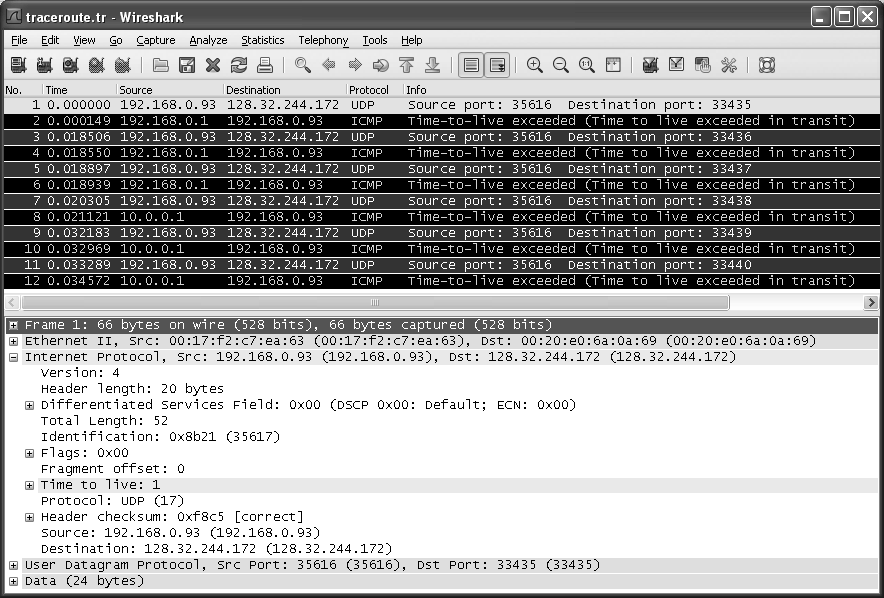
\includegraphics[width=0.7\textwidth]{imgs/8/8-12.png}
	\caption{使用IPv4 的traceroute 以发送一个TTL=1的UDP/IPv4数据报到目的端口号33435开始。在加1和重试之前每个 TTL值将被尝试3次。每个到期数据报导致在恰当跳数距离的路由器发送一个ICMPv4 超时报文返回源头。报文的源地址是“面对”发送者一方的路由器的接口地址}
\end{figure}

在图8-12中,我们能够看到 traceroute发送了6个数据报,每个数据报是按顺序发
送到目的端口号的,以33435开始。如果我们仔细观察会发现,前三个发送的数据报的
TTL = 1,第二组发送的三个数据报的TTL=2。图8-12显示了第一个。每个数据报会导致
发送一个 ICMPv4超时(代码0)报文。前三个是从路由器 N3(IPv4地址192.168.0.1)发出
的,后三个是从路由器N2(IPv4地址 10.0.0.1)发出的。图8-13显示了最后一个ICMP 报
文的详细信息。

这是此追踪的最终ICMP超时报文。它包含了在N2接收时看到的原始的IPv4数据报
(包11)。该数据报到达的时候其TTL=1,但是在递减之后值太小了,以至于 N2 不能执行
额外转发到128.32.244.172的操作。因此,N2向原始数据报的源地址发送一个超时报文。
\begin{figure}[!htb]
	\centering
	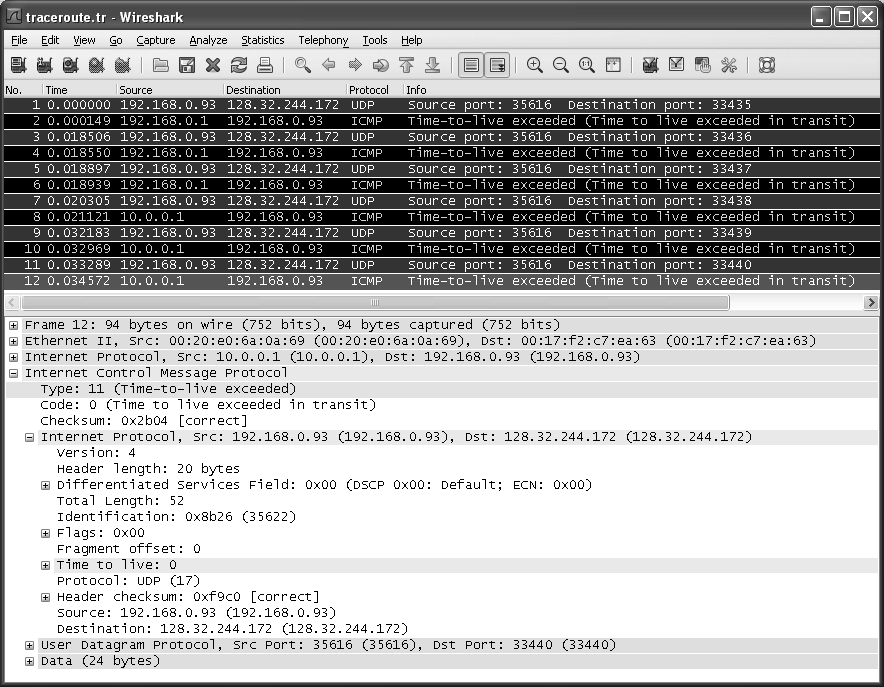
\includegraphics[width=0.7\textwidth]{imgs/8/8-13.png}
	\caption{此追踪中的最后一个 ICMPv4 超时报文是由路由器N2(IPv4地址是10.0.0.1)发出的。它包含了导致产生超时报文的原始数据报的一个拷贝。内部IPv4头部的 TTL字段为0,这是因为N2 将其从1减为0}
\end{figure}

\subsection{参数问题(ICMPv4类型 12,ICMPV6 类型4)}

当一个主机或者路由器接收到一个 IP 数据报,其IP 头部存在不可修复的问题时便会产
生一个ICMP参数问题报文。当一个数据报不能够被处理,且没有其他的ICMP报文来描述
这个问题时,这个报文充当了一个“包罗万象”的错误状态指示器。在ICMPV4 和 ICMPV6
中,当头部中某个字段超过可接受范围导致了一个错误时,一个特殊的ICMP差错报文指
针 (Pointer)字段指示了错误字段相对于出错IP 头部的偏移值。以ICMPv4 为例,指针字
段值为1表示一个错误的IPv4 DS 字段或者ECN字段(这些字段以前称IPv4服务类型
(Type of Service) 或者ToS 字节(ToS Byte),但已经被重新定义和命名过了。参见第5章)。
ICMPv4 的参数问题报文格式如图8-14所示。

代码0是ICMP参数问题报文最为常见的变体,可用于 IPv4头部中出现的任何问题,
尽管当头部或者数据报的总长度字段出现问题时可能会产生代码为2的报文。代码1以前被
用于指示数据包中缺少例如安全标志之类的选项,但目前已经不用了。代码2是最近才定
义的代码,指示存在一个损坏了的IHL 或者总长度字段值(参见第5章)。这个差错报文的
ICMPv6 版本如图8-15所示。

在ICMPv6中,相对于ICMPv4版本,差错的对待方式在某种程度上已经被重新定义
为三种情况:存在错误的头部字段(代码0),存在无法识别的下一个头部(Next Header)类
型(代码1),存在无法识别的IPv6选项(代码2)。与ICMPv4中对应的差错报文一样,
ICMPv6 参数问题中的指针字段给出了相对于问题IPv6 头部的字节偏移。例如,指针字段值
为40 指示第一个IPv6 的扩展头部中存在问题。

图8-14 当没有其他报文可应用时便采用ICMPv4 参数问题报文。指针字段指示了出错的IPv4头部中
出问题的值的字节索引。代码0是为最常见的。代码1以前用于指示缺失了一个必需的选项,
但现在已成为历史了。代码2指示出错的IPv4数据报存在一个错误的IHL 或者总长度(Total
Length)字段

图8-15 ICMPv6 参数问题报文。指针字段给出了相对于发生错误的原始数据报的字节偏移。代码0
表示一个出错的头部字段。代码1表示一个未识别的下一个头部类型,代码2表示出现了一
个未知的IPv6选项

当IPv6 头部中的某个字段包含了一个非法的值时,会导致错误头部(代码0)差错发
生。如果IPv6 下一个头部(头部链)学段包含了一个IPv6实现并不支持的头部类型值的话,
会导致代码为1的差错发生。最终,当收到一个无法识别的IPv6 头部选项时,会导致代码
为2的差错发生。

\section{ICMP 查询/ 信息类报文}

尽管ICMP 定义了一定数量的查询报文,例如地址掩码请求/应答(类型17/18)、时间
戳请求/应答(类型13/14)、信息请求/应答(类型15/16),但是这些功能已经被其他特殊
目的的协议替代(包括 DHCP,参见第6章)。唯一保存下来的广泛使用的ICMP 查询/信息
类报文是回显请求/应答报文,通常称为 ping,以及路由器发现报文。虽然路由器发现机制
在 IPv4 中并未广泛使用,但是与之类似的功能(邻居发现中的一部分)在IPv6 中却是基本
的。此外,ICMPv6 已经被扩展用于支持移动IPv6和具备组播能力的路由器发现。在本节中,
我们将探讨回显请求/ 应答功能,以及用于基本路由器及组播侦听发现(参见第6和9章)
的报文。在接下来的节中,我们将探索 IPv6 中的邻居发现操作。

\subsection{回显请求 / 应答(ping)(ICMPv4 类型 0/8,ICMPv6 类型 129/128)}
一种最为常用的ICMP报文对就是回显请求和回显应答(或者回复)。在ICMPv4 中,
它们的类型分别是8和0,在ICMPv6中它们的类型分别是128 和129。ICMP 的回显请求
报文大小几乎是任意的(受限于最终封装的IP数据报的大小)。收到ICMP 回显请求报文后,
ICMP的实现要求将任何接收到的数据返回给发送者,即使涉及多个IP 分片。ICMP 的回显
请求/ 应答报文格式如图8-16所示。

图8-16 ICMPv4 和ICMPv6 回显请求和回显应答报文格式。请求中的任何可选数据都必须包含在应
答中。NAT使用其中的标识符字段来匹配请求和应答,正如在第7章中讨论的那样
与其他ICMP 查询/信息类报文一样,服务器必须在回复中包含标识符(Identifier) 和序
列号(Sequence Number)字段。

这些报文是通过一个 ping 程序发送的,该程序通常被用于确定 Internet 上的一台主机是
否可达。如果你一度能够“ping”到一台主机,那么几乎确定能够通过其他的方法(远程登
录,其他服务等)访问到它。然而,当和防火墻一起使用时,这就不能完全确定了。

\begin{tcolorbox}
	程序名ping源自于声呐系统中定位物体。ping 程序是 Mike Muuss 编写的,
	他同时也维护了一个有趣的网页来描述它的历史 [PING]。
\end{tcolorbox}

在ping的实现中将ICMP报文的标识符字段设置为某个数,发送主机能够利用它来分
离返回的应答。在基于UNIX的系统中,例如,发送进程的进程ID 通常被放置在标识符字
段。如果有多个 ping 在同一台主机同时运行的话,这样将允许 ping 应用程序识别返回的应
答,因为ICMP 协议不像传输层协议那样有端口号。当涉及防火墙行为时(参见第7章),这
个字段通常被称为查询标识符(Query Identifier)字段。

当一个新的 ping 实例运行时,序列号字段从0开始,并且每发送一个回显请求报文便
增加1。ping 打印出每个返回的数据包的序列号,方便用户查看数据包是否丢失、重排或者
重复了。回忆一下,IP(因此ICMP也是)是一个尽力(best-effort)数据报传递服务,所以
三者中的任何一种情况都有可能发生。但是,ICMP 拥有IP 没有提供的数据校验和。

ping 程序也在传出的回显请求中的可选数据区域中包含了一份本地时间拷贝。这个时间
和数据区域中剩余的内容均包含在返回的回显应答报文中。当应答收到时,ping 程序注意到
了当前时间,用它减去应答中的时间,便得到了一个到达被 ping 的主机的 RTT估计值。由
于只用到了原始发送者的当前时间,因此这个特征不会涉及发送者和接收者之间的时钟同
步。工具 traceroute 中RTT的测量也采用了类似的方法。

先前版本的 ping 程序每秒发送一个回显请求报文,并打印出每个返回的应答。但是,
新的实现增加了输出格式和行为的变化。在Windows 中,默认是发送4个回显请求,每秒
一个,输出一些统计信息,然后退出。-t选项允许 Windows 中的ping程序不断地发送回显
请求直到被用户停止为止。在Linux中,其行就按传统那样—默认是不停运行直到被用
户中断为止。这些年有许多别的ping 变体被开发出来,且有许多别的标准选项。使用某些版
本的ping,可以构建一个包含特殊数据模式的大数据包。这已经被用于在网络通信设备中寻
找依赖于数据的错误。

在下面的例子中,我们发送一个ICMPv4 回显请求到子网广播地址。这个特定版本的
ping 程序(Linux)需要我们使用-b标志指示使用广播地址确实是我们的真实意图(如果没
有该标志将会给出一个警告,因这将会产生大量的网络流量):

\begin{verbatim}
	
Linux8 ping -b 10.0.0.127

WARNING:pinging

broadcast

address

PING 10.0.0.127(10.0.0.127)

from

10.0.0.1:56(84)bytes of data.

64 bytes from

10.0.0.1:icmp\_seg=0 tt1=255

time=1.290 msec

64 bytes from

10.0.0.6:icmp\_seq=0 tt1=64 time=1.853 msec(DUP!)

64 bytes from

10.0.0.47:icmp\_seq=0 tt1=64 time=2.311 msec (DUR!)

64 bytes from

10.0.0.1: icmp\_seq=1 tt1=255

time=382 usec

64 bytes from

10.0.0.6:icmp\_seg=1 tt1=64 time=1.587 msec (DUP!)

64 bytes

from

10.0.0.47:icmp\_seg=1 tt1=64 time=2.406 msec (DUP!)

64 bytes

from

10.0.0.1:icmp\_seg=2 tt1=255 time=380 usec

64 bytes

from 10.0.0.6: icmp\_seq=2 tt1=64 time=1.573 msec(DUP!)

64 bytes

from

10.0.0.47:icmp\_seg=2 tt1=64 time=2.394 msec (DUP!)

64 bytes from

10.0.0.1:icmp\_seq=3 tt1=255 time=389 usec

64 bytes from 10.0.0.6: icmp\_seq=3 tt1=64 time=1.583 msec(DUP!)

64 bytes from 10.0.0.47:icmp\_seg=3 tt1=64 time=2.403 msec(DUP!)

--- 10.0.0.127 ping statistics ---

4 packets transmitted,4 Packets received,

+8 duplicates, 08 packet loss

round-trip min/avg/max/mdev = 0.380/1.545/2.406/0.765 ms
\end{verbatim}

此处,4个传出的回显请求报文被发送出去,我们看到了12个应答。这个行对于采用
广播地址是非常典型的:所有接收节点必须回应。因此,我们看到序列号0、1、2和3,但
是其中每个有3个应答。这个(DUP!)符号表示回显应答中包含的序列号字段和之前接收
到的一样。由于 TTL 值是不同的(255和64),这表明不同类型的计算机正在响应。

注意这个过程(向IPv4的广播地址发送回显请求)能用于快速广播本主机系统的 ARP
表(参见第4章)。这些系统响应回显请求报文,构建一个目的是请求发送者的回显应答报
文。当响应的目标系统位于同一个子网内时,将会触发 ARP 请求查找请求发送者的链路层
地址。这么做,ARP将会在每个响应者和请求发送者之间交换。这也导致回显请求报文的
发送者学习所有响应者的链路层地址。在这个例子中,即使本系统没有关于地址10.0.0.1、
10.0.0.6、10.0.0.47的链路层地址映射,在广播之后便都会出现在ARP 表中。向发送到广播
地址的请求回复ICMP应答报文是可选的。默认情况下,Linux 系统会响应,而Windows XP
系统则不会。

\subsection{路由器发现:路由器请求和通告(ICMPv4类型9,10)}
在第6章,我们看到了 DHCP 是如何被一个主机用于获取IP 地址和学习到附近存在的
路由器的。我们提到的另外一种学习路由器的方式是路由器发现(Router Discovery,RD)。
尽管可以指定为IPv4 和IPv6主机配置,但是由于DHCP 的普及,它在IPv4 中并没有被广
泛使用。但是,目前它被指定与移动IP一起使用,因此我们简要描述一下。这个IPv6版本
构成了 IPv6 SLAAC功能的一部分(参见第6章),在逻辑上是IPv6ND 的一部分。因此,我
们在8.5 节更为广泛的 ND上下文环境中讨论它。

IPv4 的路由器发现是通过采用一对ICMPv4信息类报文实现的[RFC1256]:路由器请求
(RS,类型10)和路由器通告(RA,类型9)。通告由路由器通过两种方法发送。首先,它
们定期对本地网络(使用TTL =1)的所有主机组播地址(224.0.0.1)进行组播,并提供给
有需要的主机,它们通常使用 RS报文进行请求。使用组播将RS报文发送到所有路由器组
播地址上(224.0.0.2)。路由器发现的主要目的是让一台主机学习到它所在的本地子网中的
所有路由器,因此它能够从中选择一台作为默认路由。它也被用于发现那些愿意充当移动IP
代理的路由器。参见第9章中关于本地网络组播中的详细内容。图8-17给出了 ICMPV4 RA
报文格式,其中包含了一个 IPv4 地址列表可用做主机的默认路由器。

图 8-17 ICMPv4 路由器通告报文包含了一个IPv4地址列表可用作下一跳的默认路由。优先水平允许
网络操作人员为这个列表安排不同的优先级(越高优先级越大)。移动 IPV4[RFC5944]通过扩
展增强了 RA 报文,目的是为了通告MIPv4 移动代理以及被通告的路由器地址的前缀长度

在图8-17中,地址数(Number of Address)学段给出了报文中路由地址块的个数。每个
块包含了一个IPv4 地址及相应的优先水平(preference level)。地址条目大小(Address Entry
Size)字段给出了每个块的32位字数(在这个例子中是2)。生命周期(Lifetime)字段给出
了地址列表被认为是有效的秒数。优先水平是一个32位的有符号二进制补码整数,其值越
大代表优先级越高。默认的优先水平是0,特殊值 0x80000000表示这个地址不应该用作有
效的默认路由。

RA 报文也被移动 IP[RFC5944]中的节点用于定位一个移动(即本地和/或外地)代理。
图8-17描述了一个路由器通告报文,其中包含了一个移动代理通告扩展。这个扩展遵循传
统的RA 信息并包含一个值为16的类型(Type)字段,以及一个给出了扩展区域(不包括类
型和长度字段)内字节个数的长度(Length)字段。它的值等于(6+4K),假设包含了K个
地址。序列号字段给出了自从初始化之后代理产生的这种扩展的个数。注册字段给出了发送
代理愿意接受 MIPv4注册的最大秒数(OxFFFF 的表示无穷大)。存在具有以下含义的标志
(Flag)位字段:R(为MIP服务所需的注册),B(代理太忙无法接受新注册),H(代理愿意
充当本地代理),F(代理愿意充当外地代理),M(支持最小封装格式[RFC2004]),G(代理
支持封装数据报的GRE 隧道),r(保留零),T(支持反向隧道[RFC3024]),U(支持UDP的
隧道[RFC3519]),X(支持撤销注册[RFC3543]),1(外地代理支持区域注册 [RFC4857])。

除了移动代理通告扩展,还有一个扩展已经被设计用于帮助移动节点。前缀长度扩展
可能位于移动代理通告扩展之后,表示在基本路由器通告中每个对应的路由器地址的前缀长
度。其格式如图8-18所示。

图8-18 ICMPv4可选RA 前缀长度扩展给出了报文中基本路由器通告部分中 N个路由器地址中每个
的显著前缀位数。如果移动代理通告扩展存在的话,这个扩展紧随其后

在图8-18中,长度字段被设置等于N,即来源于基本 RA报文中的地址数字段。每
个8位的前缀长度(Prefix Length)字段给出了在本地子网中使用的路由器地址(Router
Address)字段(图8-17)对应的位数。这个扩展能被移动节点用来确定它是否已经从一个网
络移动到另一个了。采用[RFC5944]中的算法2,一个移动节点也能缓存一个特定链路上可
用的前缀集合。如果网络前缀集合已经改变,就能检测到是移动了。

\subsection{本地代理地址发现请求 / 应答(ICMPV6 类型 144/145)}
[RFC6275]定义了4种支持 MIPv6 的ICMPv6报文。其中2个ICMPv6报文用于动态本
地代理地址发现,另外2个用于重新编号和移动配置。当一个 MIPv6 节点访问一个新的网络
时,它使用本地代理地址发现请求报文动态地发现一个本地代理(参见图8-19)。

为了本地前缀,报文被发送到MIPv6本地代理的任播地址。IPv6的源地址通常是移动节点从当前正在访问的
网络上获取的地址(参见第5章)。愿意为给定节点及它的本地前缀充当本地代理的节点会发送一个本地代理地址发现
应答报文(参见图 8-20)。

图8-19 MIPv6本地代理主机发现请求报文包含的标识符将在响应中返回。为了移动节点的本地前
缀,它将被发送到本地代理的任播地址

图8-20 MIPv6本地代理地址发现应答报文包含了来源于对应的请求中的标识符,以及愿意为移动节
点转发数据包的本地代理的一个或者多个地址

直接提供给移动节点单播地址的本地代理地址,极有可能是个移交地址。这些报文用于
处理当一个移动节点在网络中转换但其 HA 已经变化了的情况。在重新建立一个合适的HA
之后,移动节点可能会初始化 MIPv6绑定更新(参见第5章)。

\subsection{移动前缀请求 / 通告(ICMPV6 类型 146/147)}
移动前缀请求报文(参见图8-21)是当一个节点的本地地址就要变无效时,用于从一
个HA处请求一个路由前缀更新。移动节点包含一个本地地址选项(IPv6 目的地址选项,参
见第5章),并使用 IPsec 保护请求(参见第18章)。

图 8-21 当一个移动节点离开去请求一个本地代理提供一个移动前缀通告时,
便发送 MIPv6 移动前缀请求报文

请求报文在标识符字段中包含了一个随机值,用来匹配请求与应答。它和路由器请求报
文类似,但是发送给一个移动节点的HA,而不是本地子网。在这个报文的通告形式中(参
见图8-22),封装的IPv6数据报必须包含一个类型为2的路由头部(参见第5章)。标识符
字段的值和请求报文中的标识符值一样。M(Manged Address,托管地址)字段表示主机应
该使用有状态的地址配置,并避免自动配置。O(Other,其他)字段表示一个有状态的配置
方法提供的是信息而不是地址。通告中包含了1个或者多个前缀信息选项。

图 8-22 MIPv6移动前缀通告报文。标识符字段值和请求中对应字段的值一致。M标志指示地址是由
一个有状态配置机制提供的。O标志表示除了地址之外的其他信息是由有状态的机制提供的

移动前缀通告报文是设计用来通知一个移动中的节点其本地前缀已经改变了。这个报文通
常是使用 IPsec保护的(参见第18章),主要是为了帮助移动节点免受假冒前缀通告的欺骗。前
缀信息选项使用了[RFC4861]描述的格式,包含了移动节点应该用来配置其本地地址的前缀。
\subsection{移动 IPv6 快速切换报文(ICMPV6 类型154)}
MIPv6 的一个变体 MIPv6定义了快速切换 (fast handovers) [RFC5568](称 FMIPv6)。
当一个移动节点从一个网络的接人点(AP)移动到另一个时,它指定的方法可以改善IP层的
切换延迟。这是通过在切换发生之前预测路由器和地址信息来完成的。这个协议涉及对所谓
的代理路由器(proxy router)的发现,它的行为类似于普通路由器,但是移动节点在切换到
一个的网络时需要用到。有对应的ICMPv6 代理路由器请求和通告报文(分别称为 RtSoIPr
和 PrRtAdv)。基本的RtSolPr和 PrRtAdv格式如图8-23所示。

图8-23 用于 FMIPv6 报文的通用ICMPv6报文类型。代码(Code)和子类型(Subtupe) 字段给出了
更深人的信息。请求报文使用代码0和子类型2,可能包含发送者的链路层地址和首选的下
一个接人点链路层地址(如果知道的话)作为选项。通告使用代码0~ 5和子类型3。不同的
代码值表示存在不同的选项、通告是否被请求了、前缀和路由信息是否已经改变、DHCP是
否需要处理

一个移动节点可能有关于它将来使用的AP的地址或者标识符的信息(例如,通过“扫
描”802.11 网络)。RtSoIPr报文使用代码0和子类型2,同时必须包含至少一个选项,即新
接人点链路层地址选项。这是用于指出移动节点请求的信息是关于哪个 AP的。RtSolPr报文
可能也包含一个链路层地址选项来识别源,如果知道的话。这些选项使用了IPv6 ND 选项格
式,因此我们在详细探讨 ND 时再讨论它们。

\subsection{组播侦听查询/ 报告 / 完成(ICMPV6 类型 130/131/132)}
组播侦听发现(MLD)[RFC2710][RFC3590]为采用IPv6的链路提供了组播地址管理。
它和IPv4采用的IGMP协议类似,在第9章中有描述。那一章详细地介绍了IGMP操作和
ICMPv6报文的使用。此处我们描述组成 MLD(版本1)报文的格式,包括组播侦听查询、
报告和完成报文。基本格式如图8-24所示。这些报文被发送时其 IPv6跳数限制(Hop Limit)
字段值1,并带有路由器告警逐跳IPv6选项。

MLD 的主要目的是让组播路由器了解与它们相连的每个链路上的主机使用的组播地址。
MLDv2(版本2组播侦听发现,在下一节描述)扩展了此功能,允许主机指定它们希望(或
不希望)接收流量的特定主机。组播路由器发送两种形式的 MLD 查询报文:一般(general)
的查询和特定于组播地址(multicast-address-specific)的查询。一般来说,路由器发送查询
报文,主机采用报告响应,或者是响应查询,或者是在一台主机的组播地址成员发生变化时

图 8-24 ICMPv6 MLD版本1报文都是这种形式。查询(类型130)都是通用或者特定组播地址的。
一般查询要求主机报告它们正在使用哪个组播地址,特定于地址的查询用于确定一个特定
的地址是否(仍然)在使用。最大的响应时间是主机可能延迟发送响应查询报文的最大毫秒
数。对于一般的查询和针对特定报告查询的组播地址,其目的组播地址为0。对于报告(类型
131)和完成报文(类型132),它将分别包含和报告相关的地址或者不再感兴趣的地址

最大响应时间(Maximum Response Time)字段只有在查询时是非零的,它是响应查询
主机发送报告可能推迟的最大毫秒数。由于组播路由器只需要知道,至少有一台主机对发往
特定组播地址的流量感兴趣(因为链路层组播支持允许路由器不必为每个目的复制报文),节
点可以随机故意地拖延它们的报告,甚至完全抑制它们(如果发现另一个邻居已经做出了响
应)。这一字段提供这种延迟时长的一个上限。对于一般的查询和路由器在报告中感兴趣的
地址,组播地址(Multicast Address)字段为0。对于 MLD 报告报文(类型131)和 MLD完
成报文(类型132),它分别包含和报告相关的地址或不再感兴趣的地址。

\subsection{版本2 组播侦听发现(ICMPV6 类型143)}
[RFC3810]定义了在[RFC2710]中描述的MLD功能扩展。特别是,它定义了一个组播
侦听的方式来指定只监听一个特定集合的发送者(或者,排除一个特定的集合)。因此,它
对支持源特定组播(SSM;参见第9章和[RFC4604][RFC4607])非常有用。它基本上是对
与IPv4一起使用的IGMPv3协议在IPv6 下使用的一个转换,它使用ICMPv6 来管理多数
组播地址。因此,我们将在这里描述报文格式,但组播地址动态的操作将在第9章中介绍。
MLDv2扩展了MLD 查询报文,增加了与特定来源相关的其他信息(见图8-25)。报文中开
始的24个字节和 MLD格式是一样的。

最大响应代码(Maximum Response Code)字段指定发送 MLD 响应报文之前允许的最大
时间。这个字段的值是特殊的,因此其解释与 MLDvI 也略有不同:如果它小于 32 768,则
与 MLDV1 中一样,最大的响应延迟就设置为该值(以毫秒为单位)。如果该值等于或大于
32769,字段使用图8-26所示的格式编码一个浮点数。

在这种情况下,最大响应时间设置为等于((mant | 0x1000)<<(exp +3))毫秒。采用这个
看似复杂的编码策略的原因是为了让大、小响应延迟值都能编码在这个字段中,并保留一
些与 MLDv1的兼容性。特别是,它可以仔细调整离开延迟,并影响报告的突发性(参见第

8-25 MLDv2 查询报文格式,它与 MLD版本1报文通用格式兼容,最大的区别是能够从主机感兴
趣列表中限制或者剔除特定的组播源

当最大响应代码字段值至少为32768时,MLDv2查询报文使用的浮点格式。在这些情况中
延迟被设置为((mant| 0x1000)<<(exp +3))毫秒

一般查询中组播地址字段设置为0。对于一个特定组播地址查询或特定的组播地址和源
询,它被设置查询的组播地址。S字段指示是否应抑制路由器端处理。设置时,它表示
王何接收的组播路由器,当监听到一个查询时它必须抑制正常的计时器更新计算。这并不表
,如果路由器本身就是一个组播监听者的话,查询器选举或正常的“主机端”处理应该初

如果设置了 QRV (Querier Robustness Variable,查询器鲁棒性变量)字段,它将包含一
个不超过7的值。如果发送者的内部QRV 值超过7,那么这个字段应设为0。在第9章介绍
的鲁棒性变量能够根据一个子网上的丢包率来微调 MLD 的更新率。QQIC (Querier’s Query
Interval Code,查询器查询间隔代码)字段编码查询时间间隔,如图8-27所示。


图8-27 MLDv2 查询器查询间隔代码编码了 MLDv2 查询之间的时间间隔。这个值的(未编码)版
本称为查询器查询间隔,且是以秒来测量的。QQ1是通过下面的方法来计算的:如果
QQIC<128,QQ1 = QQIC;否则 QQ1= ((mant | 0x10)<<(exp +3))

查询时间间隔以秒为单位,它从 QQIC字段按如下方式计算得到:如果QQIC<128,那
么 QQ1=QQIC;否则,QQ1=((mant | 0x10)<<(exp+ 3))。

源个数(Number of Sources)(N) 字段表示查询中源地址个数。对于一般的查询或者特
定的组播地址查询,此字段为0。对于特定的组播地址和源查询报文,它不为0。

MLDv2 报告中使用的组播地址记录(参见图8-28和图8-29)包含对IPv6 节点源地址过
滤器所做的修改(参见第9章关于组播在这种过滤器操作上的更多信息,描述了对特定接收
主机感兴趣或者不感兴趣的发送主机集合)。

图8-28 MLDv2 报告报文包含了一组组播地址记录向量

记录类型主要可以分为三类:当前状态(current state)记录,过滤模式变化(filter mode
change)记录和源列表改变(source list change)记录。第一类包括 MODE IS INCLUDE (IS
IN)和 MODE\_IS\_EXCLUDE (IS\_EX)类型,指明的地址过滤模式对于指定的源而言(其中
必须至少存在一个)分别是“包括”或“排除”。过滤模式变化类型 CHANGE\_TO\_INCLUDE
(TO\_IN)或CHANGE\_TO\_EXCLUDE(TO\_EX)和当前状态记录是类似的,但当有变化或
者不需要包含一个非空的源列表时将被发送。源列表改变类型,当过滤器的状态(包含/排
除)不变而只有源列表被改变时,ALLOW\_NEW\_SOURCES(ALLOW)和BLOCK\_OLD
SOURCES(BLOCK)将被使用。为了简化了MLDV2[RFC5790] 的操作,对MLDv2(和
IGMPv3)做了修改,即删除了 EXCLUDE 模式。这种“轻量级”的方法,称为LW-MLDV2
(和LW-IGMPv3),使用先前定义的相同报文格式,但删除了很少使用的要求组播路由器保存
附加状态的 EXCLUDE指令。

图8-29 一条组播地址(组)记录。MLDv2报告报文中可能存在多个这样的记录。记录类型字段
值是下列之一:MODE\_IS\_INCLUDE,MODE\_IS\_EXCLUDE, CHANGE\_TO\_INCLUDE \_MODE,
CHANGE\_TO\_EXCLUDE\_MODE, ALLOW\_NEW\_SOURCES,或BLOCK\_OLD\_SOURCES。
LW-MLDv2 通过删除 EXCLUDE 模式简化了 MLDV2。辅助数据长度(Aux Data Len) 字段包
含了记录中的辅助数据,以32位字为单位。对于在[RFC3810]中定义的MLDv2 而言,此字
段必须为 0.表示没有辅助数据

\subsection{组播路由器发现(IGMP 类型 48/49/50,ICMPV6 类型 151/152/153)}
[RFC4286] 描述组播路由器发现(Multicast Router Discovery,MRD),该方法定义的特
殊报文可以和ICMPv6 和IGMP一起使用,用来发现能够转发组播数据包和它们的一些配置
参数的路由器。最初的想法主要是和“IGMP/MLD侦听”一起使用。IGMP/MLD 侦听是一
种机制,主机和路由器(例如,第2层交换机)以外的系统也可以了解网络层组播路由器和
感兴趣主机的位置。我们将在第9章IGMP上下文中详细地讨论它。MRD报文发送时总是
将IPv4的TTL 或IPv6 的跳数限制字段设1,并设有路由器警告选项,可能是如下类型之
一:通告(151),请求(152),或终止(153)。在配置的时间间隔定期地发送通告,表明路
由器愿意转发组播流量。终止报文表明要终止这种意愿。请求报文可用于请求路由器发送通
告报文。通告报文格式如图8-30所示。

图 8-30 MRD的通告报文(ICMPv6 类型151;IGMP 类型48)包含说明多长时间发送主动通告的通
告时间间隔(秒)、发送者的查询间隔(QQI)和 MLD定义的鲁棒性变量。发送者的IP地址
就是用来指示接收者能够转发组播流量的路由器。该报文被发送到所有侦听者的组播地址
(IPV4,224.0.0.106; IPv6, ffO2::6a)

通告报文从路由器的IP地址(IPv6链路本地地址)发送到所有侦听者的IP 地址:
224.0.0.106(IPv4)和链路本地组播地址 ff02::6a(IPv6)。接收者能够了解路由器的通告间
隔和 MLD 参数(QQ1和QRV,在第9章中详细介绍)。请注意,QQ1 值是查询的间隔(以秘
计),不是之前在 MLDv2 查询中描述的QQIC(编码版本的QQ1值)。

请求和终止报文格式几乎相同(见图8-31),只有类型字段的值有所不同。

图 8-31
ICMPv6 MRD 请求(ICMPv6 类型 152;IGMP 类型 49)和终止(ICMPv6 类型153;IGMP类
型50)报文使用相同的格式。MRD报文将IPv6跳数限制字段或者IPv4 TTL 字段值设置为1,
并包含路由器警告选项。请求被发送到所有路由器的组播地址(IPv4,224.0.0.2;IPv6, ff02::2)

图8-31显示请求和终止报文的格式几乎是相同的。请求报文请求一个组播路由器发送
一个通告报文。这样的报文被发送到所有路由器地址224.0.0.2(IPv4)和本地链路组播地址
f02::2(IPv6)。终止报文被发送到所有的侦听者IP 地址,表示发送路由器不再愿意转发组
播流量了。

\section{IPV6 中的邻居发现}

IPv6中的邻居发现协议(有时简称为 NDP 或者 ND)「RFC48611将路由器发现和田
ARP提供的带有地址映射功能的ICMPv4重定向机制结合在一起。它也被指定用于支持移动
IPv6。与ARP和IPv4 普遍使用广播地址(除了路由器发现)不同,ICMPv6广泛使用组播地
址,在网络层和链路层中都使用。(回忆第2 章和第5章,IPv6 甚至没有广播地址。)

ND 被设计允许在同一个链路或者网段的节点(路由器和主机)找到彼此,确定它们之
间是否有双向连通性,确定一个邻居是否变得不合作或者不可用。它也支持无状态的地址自
动配置(参见第6章)。所有的ND功能都是由网络层或者之上的ICMPv6提供的,致使它最
大限度地独立于底层所采用的链路层技术。但是,ND 并不倾向于采用链路层组播功能(参
见第9章),也正是这个原因在非广播和非组播链路层(称为非广播多路访问或者 NBMA链
路)上的操作可能会有一些差别。

ND 中两个主要部分是:邻居请求/通告(NS/NA),在网络和链路层地址之间提供类似
于ARP的映射功能;还有路由器请求和通告(RS/RA),提供的功能包括路由器发现、移动
IP 代理发现、重定向,以及对一些自动配置的支持。ND 的一个安全变体 SEND[RFC3971]
通过引人额外的ND选项增加了认证和特殊形式的寻址。

ND报文就是ICMPv6报文,只是发送时IPv6的跳数限制字段值被设置为255。接
收者通过验证进来的ND报文有这个值,以防止被非本链路上的发送者尝试发送假冒本地
ICMPv6报文(这样的报文到达时其值会小于255)欺骗。ND报文可以携带丰富的选项。首
先我们讨论主要的报文类型,然后详述可用的选项。

\subsection{ICMPv6 路由器请求和通告(ICMPV6 类型 133,134)}
路由器通告(RA)报文表明附近路由器的存在及其功能。它们定期被路由器发送,或者
是响应一个路由器请求(RS)报文。RS报文(参见图8-32)用于请求链路上的路由器发送
RA 报文。RS报文被发送到所有路由器组播地址 ff02::2。如果报文的发送者使用IPv6地址,
而不是未指定的地址(在自动配置过程中

0

15 16

31

使用),则应该包括一个源链路层地址选

类型(133)

代码(0)

项。对于这样的报文,这是唯一有效的

校验和

8字节

选项 [RFC4861]。

保留(0)

路由器通告(RA)报文(参见图8-33)

是由路由器发送到所有节点的组播地址

选项

(FF02:1)的,或者是发送到请求主机的

图 8-32

单播地址——如果该通告是为了响应一个

请求。RA报文通知本地主机和其他路由

器关于本地链路的有关配置细节。

ICMPv6 路由器请求报文非常简单,但是通

常包含一个源链路层地址选项(不像ICMPv4

中的对应项)。假如链路中使用了一个不常用

的MTU 值,那么它可能包含一个 MTU选项

当前跳数限制(Current Hop Limit)

字段指定主机发送IPv6数据报的默认跳数限制。值为0表示发送路由器并不关心。下一个
字节包含了位字段数,正如在[RFC5175] 总结和扩展的那样。M(托管)字段表明本地 IPv6
地址分配是由有状态的配置来处理的,主机应避免使用无状态的自动配置。0(其他)字段
表示其他有状态的信息(即 IPv6地址以外的)使用一个有状态的配置机制(见第6章)。H(本
地代理)字段表示发送路由器愿意充当一个移动IPv6 节点的本地代理。Pref(优先级)字段
给出了将报文发送者作为一个默认路由器来使用的优先级层次:01,高;00,中(默认);
11,低;10,保留(未使用)。有关这一字段的更多细节在「RFC41911中有描述。当和实验
性质的ND代理工具[RFC4389]配合使用时,将使用P(代理)标志。它为IPv6 提供了一个
类似代理 ARP的功能(见第4章)。

0

15 16

31

类型(134)

当前跳数限制

校验和

路由器生命周期

代码(0)

MOHPrefP

保留

1(0)

可达时间

重传计时器

图8-33

选项

:

一个ICMPv6路由器通告报文被发送到所有节点的组播地址(02 :1)。接收节点检查以确
定跳数限制字段值是255,并确保数据包尚未通过路由器转发。报文包括三个标志:M(托管
地址配置),O(其他有状态的配置)和H(本地代理)

路由器生命周期(Router Lifetime)字段表示发送路由器可以作为默认下一跳的时间,
以秒计。如果它被设置为0,发送路由器不应该用作默认路由器。此字段只适用于使用发
送路由器作为默认路由器,它不会影响同一个报文中的其他选项。可达时间(Reachable
Time)字段给出一个节点到达另一个节点所需的毫秒数,假设已经发生了双向通信。这被
邻居不可达检测(Neighbor Unreachability Detection) 机制使用(见8.5.4节)。重传计时器
(Retransmission Timer)字段规定主机延迟发送连续ND报文的时间,以毫秒为单位。

此报文通常包含源链路层选项(如果适用的话),如果链路中使用了可变长度的MTU则
应包含MTU选项。该路由器还应该包括前缀信息选项,表示本地链路上使用了哪些IPv6前
缀。第6章包含了一个如何使用RS和RA 报文(例如,参见图6-24和图6-25)的例子。

\subsection{ICMPV6邻居请求和通告(ICMPV6 类型 135,136)}
ICMPv6 中的邻居请求(NS)报文(参见图8-34),有效地取代了IPv4 中的ARP请求报

文。其主要目的是将IPv6地址转换为链路层地址。但是,它也被用于检测附近的节点是否
可达,它们是否可以双向到达(即节点间是否可以互相通信)。当用于确定地址映射时,它
被发送到目标地址(Target Address)字段中包含的IPv6地址所对应的请求节点的组播地址
(前缀f02::1:/104,并结合请求IPv6地址中的低24位)。关于如何使用请求节点组播寻址的
更多细节,请参阅第9章。当这个报文被用来确定到邻居的连接性时,它被发送到该邻居的
IPv6 单播地址,而不是请求节点的地址。

NS报文包含发送者想设法学习的链路层地址对应的IPv6地址。该报文可能包含源链路

层地址选项。当请求是被发送到一个组播地址时,该选项必须包含在使用链路层寻址的网络
中,对于单播请求而言,该选项应该被包含。如果报文的发送者使用未指定的地址作为源地
址(例如,在重复地址检测期间),则不应该包括该选项。

ICMPv6 邻居通告(NA)报文(参见图8-35)和IPv4 中的ARP 响应报文的目的一样,

还能够有助于邻居不可达检测(见8.5.4节)。它要么作NS报文的响应被发送,要么当一
个节点的IPv6地址变化时被异步发送。它要么被发送到请求节点的单播地址,要么当请》

节点使用未指定的地址作为源地址时,它被发送到所有节点的组播地址。

ICMPV4和ICMPv6:Internet 控制报文协议

281

0

类型(135)

代码(0)

15 16

保留(0)

31

校验和

24字节

目标地址

(正被请求的 IPv6地址)

选项(如果有的话)

图8-34 ICMPv6 邻居请求报文和 RS报文类似,但包含一个目标IPv6地址。这些报文被发送到请求
节点组播地址以提供类似于 ARP的功能,发送到单播地址以测试到其他节点的可达性。在使

用低层寻址的链路上,NS报文包含源链路层地址选项


图 8-35

ICMPv6邻居通告报文包含以下标志:R表示发送者是一个路由器,S表示通告是为了响应一
个请求,O表示该报文的内容应覆盖其他缓存的地址映射。目标地址字段包含报文发送者的
IPv6地址(一般,从ND 请求中请求节点的单播地址)。包含一个目标链路层地址选项用于为
IPv6启用类似的ARP 功能

R(路由器)字段表示该报文的发送者是一个路由器。这可能会改变,例如当一台路由
器不再是路由器,而成为一台主机时。S(请求)字段表示该报文是在响应先前收到的请求。
这个字段用来验证已经取得的邻居之间的双向连通性。0(覆盖)字段表示在报文中的信息
应覆盖报文发送者之前缓存的任何信息。它不应该在请求通告、任播地址或请求代理通告中
设置,而应该在其他通告(请求或主动)中设置。

对于请求通告,目标地址字段就是正在被查找的IPv6地址。对于主动通告,它是已经
改变的链路层地址对应的IPv6地址。当通告是通过一个组播地址被请求时,此报文必须包
含支持链路层寻址的网络的目标链路层地址。我们现在来看一个简单的例子。

例子

在这里我们看到ICMPv6 回显请求/应答与ND一起使用的结果。发送者是一台启用了

IPv6 的Windows XP 系统,在附近的Linux 系统上捕获数据包。为清晰起见,有些行已被隐藏。
\begin{verbatim}
    
C:\> ping6 -s fe80::210:18ff:fe00:100b fe8o::211:11ff:fe6f:c603

Pinging fe8O::211:1lff:fe6f:c603

from fe80::210:18ff:fe00:100b with 32 bytes of data:

Reply from fe80::211:11ff:fe6f:c603: bytes=32 time<1ms

Reply from

fe80::211:11ff:fe6f:c603: bytes=32 time<1ms

Reply from fe8O::211:11ff:fe6f:c603:bytes=32 time<1ms

Reply from fe80::211:11ff:fe6f:c603:bytes=32 time<1ms

Ping statistics for fe80::211:11ff:fe6f:c603:

Packets: Sent = 4, Received = 4,Lost = 0 (08 10ss),

Approximate round trip times in milli-seconds:

Minimum = Oms,Maximum = 0ms,Average =0ms

Linux# tcpdump -i etho -$1500 -w -P ip6

tcpdump:1istening on ethO,

1ink-type EN1 OMB (Ethernet),capture size 1500 bytes

1 21:22:01.389656 fe80::211:11ff:fe6f:c603 > Ef02::1:ff00:100b:

[icmp6 sum ok]icmp6:neighbor sol: who has

fe80::210:18ff:fe0o:100b

(srC 1laddr: 00:11:11:6f:c6:03)

(len 32,hlim 255)

2 21:22:01.389845 fe80::210:18ff:fe00:100b > fe80::211:11ff:fe6f:c603:

[icmp6 sum ok] icmp6: neighbor adv:tgt is

fe80::210:18ff:fe00:100b(SO)

(tgt 1laddr: 00:10:18:00:10:0b)

(len 32,hlim 255)

3 21:22:02.390713 fe80::210:18ff:fe00:100b > fe80::211:11ff:fe6f:c603:

[icmp6 sum ok]icmp6: echo request seg 18

(len 40,hlim 128)

4 21:22:02.390780 fe80::211:11ff:fe6f:c603 > fe80::210:18ff:fe00:100b:

[icmp6 sum ok]icmp6:echo reply seg 18

(len 40,hlim 64)

continues
\end{verbatim}

Windows XP 和 Linux 均提供了 ping6程序(最近版本的 Windows 将 IPv6功能纳人常规
的ping 程序)。-s选项告诉它使用的源地址。回想一下在IPv6 中一个主机可能有可供选择
的多个地址,在这里我们选择了一个链路本地地址 fe80::211:11ff:fe6f:c603。跟踪显示了 NS/
NA 交换和一个ICMP 回应请求/应答对。通过观察可知所有 ND 报文的IPv6跳数限制字段
值为255,ICMPv6 回显请求和回显应答报文使用的值为128或64。

NS报文被发送到组播地址 f02:1:f800:100b,就是被请求的IPv6 地址 (fe80:210:18ff:fe00:
100b)对应的请求节点的组播地址。我们看到请求节点在源链路层地址选项中还包括它自己
的链路层地址 00:11:11:6f:c6:03。

NA应答报文使用链路层(和IP 层)单播地址被发送回请求节点。目标地址字段包含请
求报文中请求的值:fe80::210:18ff:fe00:100b。此外,我们还看到S和O标志字段被设置,
表示该通告为了响应先前的请求,所提供的信息应该覆盖其他任何请求节点可能缓存的信
息。R 标志字段并未设置,表示响应的主机并不充当路由器。最后,请求节点包括在目标链
路层地址选项中最重要的信息:请求节点的链路层地址 00:10:18:00:10:0b。

\subsection{ICMPV6 反向邻居发现请求/通告(ICMPV6 类型141/142)}

IPv6[RFC3122] 中的反向邻居发现(Inverse Neighbor Discovery,IND) 功能起源于需要
在帧中继网络中确定给定的链路层地址对应的IPv6地址。它类似于反向的ARP 协议,主要
用于支持IPv4网络中的无盘计算机。其主要功能是确定一个已知的链路层地址对应的网络
层地址。图8-36显示了 IND 请求和通告报文的基本格式。

IND 请求报文被发送到IPv6层的

0

15 16

31

所有节点的组播地址,但是却封装在

一个单播链路层地址(正在被查找的那

类型

(141或142)

代码(0)

校验和

8字节

个)中。它必须同时包含源链路层地址

保留(0)

选项和目的链路层地址选项。它可能

选项

…

也包含一个源/目标地址列表选项和/

或一个MTU选项。

图8-36 ICMPv6 IND 请求(类型 141)和通告(类型142)

报文的基本格式相同。它们被用于从已知的链路

\subsection{邻居不可达检测}
层地址映射到 IPV6地址

ND 的一个重要特征是检测在同一个链路上的两个系统什么时候丢失了或者变得非
对称了(即在两个方向上均不可用)。这是通过邻居不可达检测(Neighbor Unreachability
Detection,NUD)算法完成的。它被用于管理每个节点上的邻居缓存(neighbor cache)。邻
居缓存和第4章中描述的 ARP缓存类似,它是一个(概念上)数据结构,用于保存IPv6到
链路层地址的映射信息(这些信息在执行到链路邻居的IPv6数据报直接交付时需要),以及
针对映射状态的信息。图8-37显示了它如何在邻居缓存中维护条目。

•-发送的

数据包

超时

确i

你

超时

失败

(删除条目)

达到最多尝试次数

(MAX\_UNICAST\_SOLICIT)

发送NS

每 RetransTimer 毫秒重复

INCOMPLETE

主动证据

超时

(可到达时间)

STALE

PROBE

主动证据

REACHABLE

发送的

第一个

数据包

确认

DELAY

超时

(DELAY\_FIRST\_PROBE\_TIME)

确认

图8-37 邻居不可达检测帮助维护由多个邻居条目组成的邻居缓存。在任何时间,每个条目是5种状
态中的一种。对连接可达性的确认是通过接收邻居通告报文或者其他更高层的协议信息来完
成的。主动证据包括主动的邻居和路由器通告报文

每个映射可能是如下5个状态中的一种:INCOMPLETE, REACHABLE, STALE, DELAY,
PROBE。图8-37所示的转换图显示的初始状态是 INCOMPLETE 或 STALE。当一个 IPv6 节点
有一个单播数据报需要发送到目的地时,它会检查其目标缓存(destination cache),看一看对应
于目的地的条目是否存在。如果存在且目的地是在链路上的,再查看邻居缓存,确定邻居状态
是否是 REACHABLE。如果是,使用直接交付方式发送数据报(见第5章)。如果没有邻居缓存
条目,但目标似乎是在链路上,NUD 会进入 INCOMPLETE状态,并发送一个NS报文。成功
收到一个请求 NA报文便可以确定该节点是可达的,条目进入 REACHABLE 状态。STALE 状态
对应于目前还未确认的无效条目。当一个条目之前是 REACHABLE 状态但已有一段时间没有
更新,或者收到主动报文时(例如,一个节点改变其地址并发送主动 NA报文),它就进人这
个状态。这些情况表明,有可能是可达的,但仍需要一个有效的NA 来确认。

其他状态 DELAY 和 PROBE 是临时状态。DELAY 被用于当一个数据包已经被发送了,
但ND目前尚无证据表明可能是可达的情况。该状态给上层协议一个机会来提供更多的证
据。如果在 DBLAY \_FIRST\_PROBE\_TIME 秒(常数)后仍然没有接收到证据,状态将会改
变到 PROBE。在PROBE状态,ND 会定期发送NS报文(每 RetransTimer 毫秒,常数默认
值 RETRANS\_TIMER 等于1000)。如果在发送 MAX\_UNICAST\_SOLICIT(预设为3)个
NS报文后还未收到任何证据,就应该删除该条目。

\subsection{安全邻居发现}
SEND(安全邻居发现)[RFC3971]是一组特殊的增强功能,旨在为ND报文提供额外的
安全性。这是为了帮助抵制各种欺骗攻击,其中一台主机或路由器可能会伪装成另一个(更
多细节见第18章、8.6节和 [RFC3756])。特别是在响应NS报文时,它防止节点伪装成其他
节点。SEND 不使用IPsec(见第18章),它有自身的特殊机制。这种机制也可用于确保安全
的 FMIPv6 切换 [RFC5269]。

SEND在一套假设的框架中操作。首先,每个具备SEND的路由器有一个证书

(certificate) 或密码认证,它可以用来证明一台主机的身份。接下来,每个主机还配备了一个
信任锚(trust anchor)—一配置信息可以用来验证证书的有效性。最后,每个节点在配置它
将使用的IPv6地址时,将会生成一个公钥/私钥对。第18章将对证书、信任锚、密钥对以
及其他相关的安全技术进行详细介绍。

\subsubsection{密码生成地址}
也许 SEND 最有趣的特征是使用完全不同类型的称密码生成的地址(Cryptographically
Generated Address, CGA)[RFC3972][RFC4581][RFC4982] 的IPv6地址。这种类型的地址是
基于节点的公钥信息,从而将地址和节点证书关联起来。因此,拥有相应的私钥的节点或地
址的所有者能够证明它是一个特定CGA 的授权用户。CGA 也编码与它们相关联的子网前缀,
因此它们不能被轻易地从一个子网转移到另一个子网。这种做法与通常分配地址的方法完全
不同。

将一个64位的子网前缀和一个特殊构造的接口标识符相“或”,便生成了一个IPv6
CGA。CGA 接口标识符是通过一个称为Hashl 的安全散列函数(secure hash function)计
算出来的(被认为难以反转的散列函数,参见第18章),它的输入是节点的公钥和一个特殊
的CGA 参数数据结构。这些参数也被用来作为另一个安全散列函数 Hash2 的输人,它提供
了散列扩展(hash extension)技术,能有效地扩展散列函数的输出位数,进而提高其安全
性(即生成一个不同的输人但却有相同散列值的强度)[A03][RFC6273]。CGA 技术允许自动
生成地址所有者的公钥,所以这种方法可以在没有公钥基础设施(public key infrastructure,
PKI) 或其他可信任的第三方下工作。

CGA 参数数据结构如图8-38所示。伪随机序列(Modifier)字段初始化一个随机值,碰
撞计数(Collision Count)字段初始化次0。这个结构包括一个扩展字段(Extension Field)可
供未来使用[RFC4581]。

0

31

碰撞计数

15 16

伪随机序列

(16字节)

子网前缀

(8字节)

公钥

(可变的)

扩展字段

(可选,可变的)

CGA 参数

子网前缀(64位)

• Hashl:最上面的64位安全散列函数

的所有字段值,包括在计算 Hash2时

发现的最终伪随机序列值。

Hash2:最上面的112位的安全散列函

数字段值,其中子网前缀和碰撞计数

零。通过增加伪随机序列字段来重新计

算 Hash2,直到最初(16*Sec)位变

0为止。

Sec(3位)

U=0/g-0

(2位)

Hashl 值(59位)

CGA

图8-38 用来计算CGA的SEND方法。CGA 参数数据结构可用作两个加密散列函数 Hashl 和 Hash2
的输入。Hash2值必须有(16*Sec)个初始0位,其中 Sec 是一个3位的参数。到Hash2适
当计算时,才改变伪随机序列字段。结果值被用来计算 Hashl,并和Sec与子网前缀结合用
来生成 CGA

一个称为 Sec 的3位无符号参数将影响该方法对数学破解的抵御力(采用了安全散列函
数[RFC4982]),以及计算中的计算复杂性(在 Sec 值中它们是指数的)。IANA 为 Sec 值维护
一个注册表[SI]。配合 Sec值,Hashl 和 Hash2 函数在相同的CGA参数块进行操作。该地
址所有者首先为伪随机序列字段选择一个随机值,将子网前缀字段看作0,再计算Hash2的
值。结果需要有(16*Sec)个初始0位,所以修改输人将伪随机序列字段递增1,并重新计
算 Hash2 直到条件满足为止。这种计算的时间复杂度为 O(216S0o),并随着Sec 的增加代价会
更高。但是,只有当最初创建地址时,这种计算才是必需的。

一旦找到适当伪随机序列字段,便用59位的Hashl值形成接口标识符的低59位。前
3位构成3位Sec 值,6~7(左起)位包含两个0位(对应于第2章中描述的u和g地址)。
如果该地址被发现存在冲突(例如,使用第6章描述的重复地址检测),递增碰撞计数字段,
并重新计算 Hash1。碰撞计数值的增长是不允许超过2的。由于地址冲突在开始时是不常见
的,当多个这样的冲突出现时应考虑是否配置错误或遭到了攻击。一旦所有必要的计算完成
了,通过连接子网前缀,Sec 值以及 Hashl值便能形成CGA。需要注意的是,如果子网前
缀改变了,只需要重新计算 Hash1,因为伪随机序列字段值仍然保持不变。(对替代 CGA 的
方法感兴趣的读者应该看看[RFC5535],它描述了基于散列的地址(hash-based address),或
HBA。HBA 用在一个稍微不同的环境中的多前缀多宿主主机中,并使用了计算复杂度较低
的不同加密形式,当然也定义了 HBA-CGA 兼容选项。)

到目前为止我们已经看到CGA 是如何产生的,但还不知道如何用于安全中。注意任
何人都可以生成一个 CGA,只要有子网前缀、Sec 值和自己的(或别人的)公钥。为了确
保CGA 格式完好,并使用了适当的子网前缀,它必须经过验证,这一过程称为CGA验证
(CGA verification)。一个验证需要CGA 和CGA 参数的知识。验证过程需要确保满足如下条
件:碰撞计数不大于2,CGA 子网前缀和CGA 参数中的前缀匹配,从CGA 参数计算出的
Hashl需要和CGA 的接口标识符部分匹配(其中开始的3位、第6位和第7位“不需要关
心”),通过值为0的子网前缀(Subnet Prefx)和碰撞计数(Collision Count)字段以及 CGA
参数计算出来的 Hash2值应该有(16*Sec)个初始的0位。如果这些检查都是成功的,就是
一个对应于子网前缀的合法CGA。这个计算最多涉及两个散列函数,这是远远比地址生成
过程简单的。

验证CGA 正在被其授权地址所有者使用,这称为签名验证(signature verification),所
有者形成了一个类型报文,并附上一个 CGA 签名,该签名是使用CGA 中的公钥及其对应的
私钥的知识计算出来的。通过将一个特的128位类型标签和报文结合起来,验证将形成一
个数据块。使用一个 RSA 签名(RSASSA-PKCSI-VL

\_5 [RFC3447]),并结合公钥(从 CGA

参数提取)、数据块和签名作为参数来验证CGA的所有权。一般来说,只有在CGA 验证和
签名验证过程都顺利完成时,CGA 及其用户才被认为是合法的。

使用ICMPv6报文和6个在[RFC3971]中定义的选项来处理CGA 和验证。RFC还定义
了2个IANA托管的注册表,用来保存信任锚选项中的名称类型(Name Type)字段和证书
选项中的证书类型(Cert Type)字段(见8.5.6.13节)。[RFC3972]定义了CGA报文类型注
册表,采用在[RFC3971]中定义的128位值(其他值是在SEND之外定义使用的)0x086FC
ASE10B200C99C8CE00164277C08。Sec 的注册值在[RFC4982]中定义,但目前只提供值0、1、
2,分别对应于在Hash2函数中使用的SHA-1 安全散列函数使用的0、16或32个初始0位。
在[RFC4581]中定义的扩展格式支持TLV 编码,可用于未来标准的扩展,但到目前为止只
定义了一个[RFCS535]。我们现在将描述两个与SEND一起使用的ICMPv6 报文,等我们在
下一节讲完所有的ICMPv6选项才讨论这些选项。

\subsubsection{证书路径请求/通告(ICMPv6 类型148/149)}
SEND定义了请求和通告报文用来帮助主机确定构成一个证书路径的证书。这被主机用

来验证路由器通告的真实性。图8-39显示

0

15 16

31

了请求报文。

类型(148)

代码(0)

证书路径请求报文包含一个随机标识

标识符

校验和

组件

符(Identifer)学段用来匹配请求和通告。

组件字段值提供了一个索引以表示请求者

感兴趣的证书路径中的点。如果需要整个

路径中的证书,这个值被设置全1(值

65535)。这个报文可能包含一个信任锚选

项(参见8.5.6.12节)。第18章详细描述了

选项

图8-39 证书路径请求报文。发送者通过由组件

(Component)字段值提供的位置索引来请

求一个特定的证书。值65535表示需要路

径中的所有证书,其中该路径的根身份在

附加信任锚选项中给定

ICMPV4和ICMPv6:Internet 控制报文协议

287

证书和证书路径。

图8-40显示的证书路径通告报文提供了在一个多组件通告中表示一个组件(证书)的方
法。这些报文为了响应一个请求而发送,或由具备SEND功能的路由器定期发送。当为了响
应请求而发送报文时,目的IPv6地址是接收者的被请求节点组播地址。

0

15 16

31

类型 (149)

代码(0)

标识符

组件

校验和

所有组件

保留(0)

选项

…

图 8-40

请求路径通告报文。发送者通过由组件字段值提供的位置索引来请求一个特定的证书。值
65535 表示需要所有根植在一个附加信任锚选项中给定身份的路径中的证书

标识符字段持有在相应的请求报文中收到的值。针对发送到所有节点组播地址的主动通

告报文,该值被设置0。所有组件字段表示在整个证书路径中的组件总数,包括信任锚。
需要注意的是推荐用一个单独的通告报文来避免分片,那么这样的报文只包含一个单一的组
件。组件字段给出了在证书路径中相关证书的索引(提供一个附加的证书选项)。在一个N
个组件的证书路径中发送通告的推荐顺序是(N-1,N-2,⋯

,0)。组件N不必被发送,因

为它已经在信任锚中。

\subsection{ICMPV6邻居发现选项}
正如IPv6家族中的许多协议,它定义了一套标准协议头部,还包含了一个或多个选项。
ND(邻居发现)报文可能包含零个或多个选项,一些选项可以出现多次。但是,对于某些报
文而言,有些选项是必需的。图8-41给出了

0

15 16

31

ND 选项的通用格式。

所有的ND选项以8位类型和8位长度字

类型

(8位)

长度

(8位)

段开始,支持长度可变的选项,最大到255字

节。选项被填充以形成8字节边界,长度字段

基于类型的内容

(可变)

给出了选项的总长度,以8字节单位。类型

和长度字段包含在长度字段的值中,最小值为

1。表8-5给出的列表包含了在2011年年中定

义的25个标准选项(加上实验值)。正式列表

图8-41 ND选项的长度是变化的,并以一个通

用的TLV 布局开始。长度字段给出了

选项的总长度,以8字节为单位(包

含类型和长度字段)

可以在[ICMP6TYPES]中找到。

类型

2

3

4

5

名

称

源链路层地址

目标链路层地址

前缀信息

被重定向的头部

MTU

表8-5 IPv6 ND选项类型、定义参考、用途和注释

参考

[RFC4861]

[RFC4861]

[RFC4861][RFC6275]

[RFC4861]

[RFC4861]

用途/注释

发送者的链路层地址;与NS、RS及RA报文一起使用

目标链路层地址;与NA及定向报文一起使用

一个 IPv6前缀或者地址;与RA报文一起使用

原始IPv6 报文的部分;与重定向报文一起使用

推荐的MTU;与RA 报文、IND通告报文一起使用

(续)

类型

6

7

8

9

10

11

12

13

14

15

16

17

19

20

24

25

26

27

28

31

253,254

名称

NMBA 捷径限制

通告间隔

本地代理信息

源地址列表

目标地址列表

CGA

RSA签名

时间截

随机数

信任锚

证书

IP 地址 /前缀

链路层地址

邻居通告确认

路由信息

递归 DNS服务器

RA 标志扩展

切换密钥请求

切换密钥应答

DNS 搜索列表

实验性

参考

[RFC2491]

[RFC6275]

[RFC6275]

[RFC3122]

[RFC3122]

[RFC3971]

[RFC3971]

[RFC3971]

[RFC3971]

[RFC3971]

[RFC3971]

[RFC5568]

[RFC5568]

[RFC5568]

[RFC4191]

[RFC6106]

[RFC5175]

[RFC5269]

[RFC5269]

[RFC6106]

[RFC4727]

用途/注释

“捷径尝试”的跳数限制;与NS报文一起使用

主动RA 报文的发送间隔;与RA报文一起使用

成为一个 MIPv6 HA 的优先级和生命周期;与RA 报文一

起使用(设置H位)

主机地址;与IND 报文一起使用

目标地址;与IND报文一起使用

基于密码的地址;与安全邻居发现报文(SEND)一起使用

主机签名的证书(SEND)

反重放时间戳(SEND)

反重放随机数(SEND)

指示证书类型(SEND)

编码一个证书(SEND)

移交或者 NAR地址;与 FMIPv6 PrRtAdv报文一起使用

想要的下一个接人点或者移动节点的地址;与FMIPV6

RtSolPr 或者 PrRtAdv 报文一起使用

告诉移动节点下一个有效的CoA;与RA 报文一起使用

路由前缀/首选的路由器列表

DNS 服务器的IP 地址;添加到 RA报文

扩展 RA 标志的空间

FMIPv6

-使用 SEND 请求密钥

FMIPv6-

使用 SEND 应答密钥

DNS域搜索名称;添加到 RA报文中

[RFC3692]类型的实验 1/2

\subsection{.1}
源/目标链路层地址选项(类型1,2)

每当在一个支持链路层选址的网络中使用时,源链路层地址选项(类型1,参见图8-42)

就应该被包含在 ICMPv6 RS 报文、NS报文和

15 16

31

RA 报文中。它指定了一个和报文相关的链路

层地址。对于含有多个地址的节点可能包含上

类型

(1或2)

长度

述的多个选项。

当响应一个组播请求时,采用类似格式的

链路层地址

(可变)

目标链路层地址选项必须包含在 NA报文中。

这个选项通常包含在重定向报文中(之前讨论

的),但当在一个 NBMA 网络上操作时则必须

被包含在这样的报文中。

图8-42 源(类型1)和目标(类型2)链路层

地址选项。长度字段值给出了整个选

项的长度,包括地址,以8字节为单

位(例如,一个 IEEE 以太网类型地址

的长度字段值应该为1)

\subsubsection{前缀信息选项(类型3)}
在RA报文和移动前缀通告报文中提供的前缀信息选项(PIO)表示链路上节点的IPv6
地址前缀和(在某些情况下)完整的IPv6地址(参见图8-43)。在多个前缀或者地址被报告
的情况下,在单个报文中可能包含多个该选项的拷贝。路由器应该包含它使用的每个前缀的
PIO。将R 位字段设置1表示前缀(Prefix)字段包含发送路由器的整个(entire)全局 IPv6
地址,而不只是将前缀中的剩余位设置为0或者是它的本地链路地址(在所包含的IPv6 数据
报的源 IP地址(Source IP Address)字段中)。这对移动 IPv6 本地代理发现将非常有用,发
送路由器通告的本地代理必须包含这个选项,其中至少为一个前缀设置 R位字段。

0

15 16

31

类型(3)

长度(4)

前缀长度

(8位)

LAR

保留1(0)

(5位)

有效生命周期(秒)

首选生命周期(秒)

保留2(0)

前缀

(128位)

图 8-43

前缀信息选项包含一个在本地网络中使用的IPv6地址前缀。如果设置了A位字段,它将为主
机提供可用于地址自动配置的前缀。L位字段表示在“在链路上”判定中允许使用该前缀。R
位字段表示所包含的前缀是发送路由器的整个全局IPv6地址

前缀长度字段给出在配置中被视为有效的前缀字段中的位数(多达128位)。L位字段是
“在链路上”的标志,并表示所提供的前缀是能用于在链路上判定的(请参阅下文)。如果没
有设置,它对在链路上判定的使用没有做任何声明。A位字段就是“自主自动配置”标志,
并表示所提供的前缀可用于自动配置(见第6章)。有效生命周期(Valid Lifetime)和首选生
命周期(Preferred Lifetime)字段分别表示前缀能被用于在链路上判定和自动地址配置的秒
数。任何一个字段中值 OxFFFFFFFF 表示无穷大。

在IPv6 中,“在链路上”的节点对应于那些能够使用直接交付到达的节点(第5章)。

在IPv4 中,节点被认为是在链路上的,如果它们有一个共同的前缀,由它们自己的IPV4
地址和分配的子网掩码组合确定。虽然使用 IPv6 就可以实现这样的安排,但并不是必需
的,未经确认“在链路上”状态不能被假设。相反,L位字段表示对一台主机或路由器而言
哪些前缀或单个主机列表是在链路上的[RFC5942]。其他机制也可以达到这个目的(例如,
DHCPv6,手工配置,或ICMPv6重定向报文)。一个节点通常被认为是不在链路上的,除非
有确认信息表明它是在链路上的。

\subsubsection{重定向头部选项(类型4)}
重定向头部选项被用于包含一份导致生成重定向报文的原始(“违规”)IPv6 数据报。

图8-44 给出了选项格式。任何其他类型的报文将忽略该选项。

\subsection{.4}
MTU选项(类型5)

MTU 选项仅在RA报文中提供,在其他地方被忽略(参见图8-45)。它提供了主机使用

的 MTU,假设能够支持一个可配置的 MTU。

0

类型(4)

15 16

长度

保留(0)

保留(0)

尽量多地包含违规数据报,只要最终的

IPv6/ICMPv6 数据报不超过最小的 MTU

31

图8-44 重定向头部选项标记出了部分(或者全部)违规IPv6 数据报拷贝的开始。
在任何情况下,该报文受限于最小的 IPv6 MTU(当前是1280字节)

0

15 16

31

类型(5)

长度(1)

保留(0)

8字节

MTU

图 8-45

MTU选项包含在本地链路中使用的 MTU。这个选项是和RA报文一起使用的,

在使用非标准或者未知 MTU 时是最有用的

MTU 选项非常重要,例如在桥接两个或者多个拥有多个不同MTU 的异构链路层技术时。

没有这个选项(假设桥接并没有产生ICMPv6PTB报文),在桥接链路层网络中主机可能无法
可靠地和其他主机通信。注意这个报文保留了32个比特位来存储 MTU,支持非常大的MTU。
\subsection{.5}
通告间隔选项(类型7)

这个选项可能被包含在RA报文中,在其他地方被忽略。它指定了主动组播路由器通告
间的最大时间间隔(参见图 8-46)。

0

31

15 16

类型(7)

长度(1)

通告间隔(毫秒)

保留(0)

8字节

图8-46 通告间隔给出了主动组播路由器通告之间间隔的毫秒数

通告间隔选项给出定期路由器通告报文间的时间。通告间隔(Advertisement Interval) 字
段定义了此报文到达网络上的发送者所发送的RA 报文传输间的最大毫秒数。路由器发送的
通告可能比选项指定的通告多,但是并不频繁。移动IPv6节点在其运动检测算法中使用此
选项[RFC6275]。

\subsubsection{本地代理信息选项(类型8)}
这个选项包含在愿意充当移动IPv6本地代理[RFC6275](即那些在RA 报文中设置H
位字段的)的路由器发出的RA 报文中,在其他的地方被忽略。如果H位字段没有被设置的
话,是不允许包含该选项的。在使用了请求 RA 报文进而多个不同的报文携带了多个地址且
设置了R位字段的情况下,它们中的每个都必须包含该选项,且包含相同的值。图8-47给
出了本地代理信息选项格式。

本地代理优先级(Home Agent Preference) 字段是一个16位无符号整数,用于帮助移动
节点预定通过“本地代理地址发现应答”报文提供给它的地址。值越大表示使用发送路由器
作为一个本地代理的优先级程度越大。如果这个选项没有被包括在H位字段(本地代理)已
经被设置的路由器通告报文中,起始路由器的优先级值被认为是0(最低的优先级)。

15 16

31

类型(8)

长度(1)

本地代理优先级

保留(0)

本地代理生命周期(秒)

8字节

图8-47 本地代理信息选项表示了选项的发送者愿意作一个移动IPv6的本地代理的优先级和时间长
度。本地代理优先级字段值越大,表示越愿意做一个本地代理。本地代理生命周期字段给出
了发送者愿意成一个 HA的秒数

本地代理生命周期(Home Agent Lifetime)字段也是16位无符号整数,指定该报文的发
送者应考虑作为本地代理(带有之前描述的相应的优先级)的秒数。此字段的默认值等于所
包含的RA报文生命周期字段。这一字段的最大值(65 535)对应18.2小时,最小值是1(0
表示不允许)。如果本地代理生命周期和本地代理优先级字段仅包含默认值,那就不允许在
RA 报文中包含整个选项。

\subsubsection{源和目标地址列表选项(类型9,10)}
这些选项可能被包含在IND报文中[RFC3122]。图8-48给出了格式。源地址列表选
项(类型9)包含了一个由源链路层地址选项指定的IPv6地址列表。目标地址列表选项(类
型10)包含了由目的链路层地址选项指定的IPv6地址列表。在选项中包含的地址个数等于
(Length-1)/2,其中长度(Length)字段值包含了选项的大小,以8字节单位。

15 16

31

类型

(9或10)

长度

保留(0)

24字节

IPv6 地址

(128位)

IPv6地址

可变

大小

IPV6 地址

图 8-48

源(类型9)和目标(类型10)地址列表选项。这些被用来支持IND,并提供了一个
节点的IPv6地址的列表。只能包含用来发送报文的接口的地址

\subsubsection{CGA选项(类型11)}
CGA选项被用来和 SEND一起携带 CGA参数,这些参数是检验器执行 CGA 验证和签
名验证所必需的。图 8-49给出了它的格式。


图8-49 与SEND一起使用的CGA选项。该选项编码了图8-38中的CGA 参数
CGA 参数部分由图8-38 描述的相同字段组成。更多的细节请参见 [RFC3971]。

\subsubsection{RSA 签名选项(类型12)}
RSA 签名选项被用来和SEND一起携带校验器能够使用的 RSA签名,将它和CGA参
数一起确定发送系统是否拥有与CGA公钥相关的私钥。图8-50给出了它的格式。


图 8-50

与SEND一起使用的RSA签名选项。该签名被编码进了 \verb|PKCS#1 v1.5|(参见第18章)格式,
被用于检验发送者拥有匹配的私钥,因此是CGA的正确拥有者

密钥散列(Key Hash)字段包含构建签名所使用的公钥经SHA-1 散列后其结果的高128
位。数字签名(Digital Signature)字段包含一个基于下面这些值的标准化签名:SEND的
CGA 报文类型标签,源IP 和目的IP地址,ICMPv6 头部的开始32位字(类型、代码和校验
和字段),ND 协议的报文头和选项(不包括 RSA签名选项)。

\subsubsection{时间戳选项(类型13)}
时间戳选项给出了发送系统知晓的当天的当前时间。这有助于避免遭到潜在的针对
SEND 的重放攻击[RFC397]。图8-51给出了它的格式。

时间戳(Timestamp) 字段记录了自1970年1月1日00:00 UTC以来的秒数。其格式是
定点的,高阶的48位编码了完整的秒数,剩下的位数表示小数秒(1/64K)的值。

0

15 16

31

类型(13)

长度(2)

保留

(48位)

16字节

时间戳

(64位;自1970年1月1日到目前的秒数)

图 8-51

与 SEND 一起使用的时间戳选项。该值编码了从 1970年1月1日

至今的秒数。主要用于防范重放攻击

\subsubsection{随机数选项(类型14)}
随机数选项保存了一个最近生成的随机数。这有助于防范潜在的针对SEND的重放攻击
[RFC3971]。图8-52 给出了它的格式。

0

15 16

31

类型(14)

长度

随机变量值

(可变,至少为6字节)

图 8-52

与 SEND 一起使用的随机数选项。该值编码了一个和 SEND报文
一起使用的随机数。它被用来防范重放攻击

随机数选项值是由发送者选择的一个随机数。数值的长度至少为6个字节。第18章详
细描述了如何使用随机数来对抗重放攻击。

\subsubsection{信任锚选项(类型15)}
信任锚选项包含了一个证书路径的名称(根)(参见第18 章)。它与SEND一起被主机用

来验证 RA 报文的真实性。图 8-53给出了它的格式。


图 8-53

与SEND一起使用的信任锚选项。信任锚是一个证书链的根的名称。后续的证书可以通过和
信任锚的比较来验证。主机利用SEND 中的信任链来验证路由器通告

名称类型(Name Type)字段表示所使用的名称类型。当前已经定义了两个值:1,DER
X.502 名称;2,全限定域名称(FQDN)。可能会包含多个信任锚。名称字段采用名称类型
字段定义的格式给出了信任锚的名称。信任锚是报文发送者愿意接受的信任链的信任根(参
\subsubsection{证书选项(类型16)}
证书选项保存了和 SEND[RFC3971]一起使用的单独证书,用以提供证书路径。图8-54
给出了它的格式。

图 8-54

与SEND 一起使用的证书选项。选项保存了一个组成证书路径上的
一个组件的加密证书。这可以用来验证路由器通告

证书类型(Cert Type)字段表示所使用的证书的类型。目前,只定义了一个值:1,
X.509v3证书。第18 章详细介绍了证书及其管理方法。

\subsubsection{IP 地址/前缀选项(类型17)}
IP 地址/前缀选项是和 FMIPv6 报文一起使用的(ICMPv6 类型 154)[RFC5568]。图
8-55 给出了它的格式。

选项代码(Option-Code)字段值表示哪种类型的地址被编码了:1,旧的移交地址;2,
新的移交地址;3,新访问路由器的(NAR的)IPv6地址;4,NAR 的前缀(在PrRtAdv中)。
前缀长度(Prefix Length)字段给出了IPv6地址(IPv6 Address)字段中有效前导位个数。
IPv6地址字段编码了由选项代码字段认定的 IPv6 地址。

0

15 16

31

类型(17)

长度(3)

选项代码

前缀长度

保留(0)

24字节

IPv6地址

(或者前缀)

417

~

418

图 8-55

与FMIPv6一起使用的IP 地址/前缀选项。该选项保存下一个访问路由器的前缀

或者IPv6地址,或者是一个移动节点使用的移交地址

\subsubsection{链路层地址选项(类型19)}
链路层地址(LLA)选项是和 FMIPv6 报文(ICMPv6 类型154)[RFC5568]一起使用的。
图8-56 给出了它的格式。

选项代码字段值表示相关的链路层地址(Link-Layer Address)字段值是如何解释的:0,
通配符,即附近所有的AP都要求解析(resolution);1,新AP 的地址;2,移动节点的地
址:3,新访问路由器的地址;4,RtSolPr/PrRtAdv 报文的源地址;5,地址是当前路由器的;
ICMPv4和ICMPv6:Internet 控制报文协议

295

6,对应到这个地址的AP没有可用的前缀信息;7,编址的AP没有可用的快速切换。链路
层地址字段包含由选项代码字段指定的地址。

0

1516

31

类型(14)

长度

选项代码

链路层地址

(可变)

图8-56 与FMIPv6一起使用的链路层地址选项。选项代码值指示和地址关联的实体(即任意AP,特
定AP,NAR,RtSolPr 的发送者或者 PrRtAdv报文,路由器),如果前缀信息可用,且LLA
中指示的 AP能够支持快速切换

\subsubsection{邻居通告确认选项(类型20)}
该选项是和 FMIPv6报文(ICMPv6类型154)[RFC5568]一起使用的。图8-57给出了

它的格式。

0

类型(20)

长度(1或3)

15 16

长度(0)

31

选项代码

状态

NCoA

(新移交地址,如果提供的话)

图 8-57

与FMIPv6一起使用的邻居通告确认选项。当一个移动节点从一个之前访问的路由器转移到

一个新的访问路由器,并想使用一个特定的新移交地址时,新路由器表示被推荐的地址的可

接受性

选项代码字段值是0。状态(Status)字段表示对主动邻居报文的处置。定义了如下值:

1,新移交地址(NCoA)是无效的(执行址配置);2,NCoA 是无效的(采用IP地址选项
中提供的NCoA);3,NCoA 是无效的(使用NAR 的地址来代替NCoA);4,之前提供的移
交地址(PCoA)(没有发送绑定更新);128,无法识别的链路层地址。

\subsubsection{路由信息选项(类型24)}
该选项与 RA报文一起使用,表示通过一个特定路由器能够到达哪些不在链路上的前缀
[RFC4191]。图 8-58 给出了它的格式。

前缀长度(Prefx Length)字段给出了前缀字段中的有效先导位的个数。前缀(Pref)字
段表示和包含的前缀相关联的路由器相对于其他路由器的优先级。如果这个字段包含值2,
选项必须被忽略。路由生命周期字段给出了前缀被认为有效的秒数。所有位都是1的值表示
无穷大。前缀(可变长度)字段给出了被描述的IPv6 前缀。

0

15 16

类型(24)

长度

31

保留(0)优先级 保留 (0)

(3位)(2位)

(3位)

前缀长度

路由生命周期(秒)

前缀

(可变长度)

8-58

路由信息选项表示使用一个特定的路由器到达一个特定的不在链路上的前缀的优先级。在同

时存在多个可用路由器且通过不同的方式到达相同目的地时,这个选项特别有用

.6.18 递归 DNS 服务器选项(类型25)

[RFC6160]中定义的递归 DNS服务器(RDNSS)选项和RA 报文一起使用,能够通过持
一个或者多个 DNS服务器的地址来增强无状态配置(参见第6 章和第11章)。一个 RA苏
中可能包含多个 RDNSS选项。图8-59给出了它的格式。

0

15 16

31

类型(25)

长度

保留(0)

生命周期(秒)

24字节

递归 DNS服务器的IPv6地址

(128位)

附加服务器的IPv6地址

可变

大小

附加服务器的 IPv6地址

图8-59

递归 DNS服务器选项表示一个或者多个能够执行递归查询的DNS服务器的IPv6地址

生命周期(Lifetime)字段给出了列表中的DNS服务器被认为是有效的时间长度,以和

,所有位都是1的值表示无穷大的生命周期。假如需要不同的生命周期,在同一个RA报
中可能包含多个不同的 RDNSS 选项。

ICMPv4 和ICMPv6:Internet 控制报文协议

297

\subsubsection{路由器通告扩展标志选项(类型26)}
这个选项扩展了 RA报文中使用的标志字段。它有时也称为扩展标志选项(Expanded
Flags Option,EFO)。图8-60给出了它的格式。

0

15 16

31

类型(26)

长度

分配可用的位字段

(可变)

图8-60 路由器通告扩展标志选项为今后定义 RA标志提供了一个任意大小的附加空间
长度(Length)字段目前被定义为1,直到后续的位被分配为止。

\subsubsection{切换密钥请求选项(类型27)}
切换密钥请求选项和 FMIPv6报文一起使用,它使用SBND保护信令信息的安全
[RFC5269]。图 8-61 给出了它的格式。

0

15 16

类型(27)

长度

填充长度

31

AT

保留(0)]

(4位)(4位)

切换密钥加密公钥

(可变)

填充(0)

(可变)

图8-61 与FMIPv6报文一起使用的切换密钥请求选项使用SEND保护信令的安全,并提供了包括一
个公钥在内的CGA 参数。路由器使用这个信息形成一个为移动节点加密好的切换密钥
填充长度(Pad Length)字段给出了在选项尾部用0填充的字节个数(包含在长度字段之
内)。算法类型(Algorithm Type,AT)字段表示用于计算认证者的算法(参见[RFCS568])。
切换密钥加密公钥(Handover Key Encryption Public Key)字段使用和CGA选项相同的格式
加密了 FMIPv6 CGA公钥。填充(Padding)字段包含了值为0的字节以保证选项的长度是8
字节的倍数。

\subsubsection{切换密钥应答选项(类型28)}
该选项和 FMIPv6报文一起使用,它使用SEND保护信令信息的安全 [RFC5269]。
图 8-62 给出了它的格式。

填充长度及AT字段和切换密钥请求选项中一样。密钥生命周期(Key Lifetime)字
段给出了切换密钥有效的秒数(默认是 HK-LIFETIME 或者43 200s)。加密的切换密钥
(Encrypted Handover Key) 字段保存了一个对称密钥(参见第18章),是经过移动节点的切
换密钥加密过的。加密格式是 RSAES-PKCS1-V1\_5[RFC3447]。填充字段包含了值为0的字
节以保证选项的长度是8字节的倍数。

420

421

0

类型(28)

长度

密钥生命周期

15 16

填充长度

AT

(4位)

保留(0)

(4位)

加密的切换密钥

(可变)

填充(0)

(可变)

图8-62 与FMIPv6报文一起使用的切换密钥应答选项使用SBND保护信令的安全,并提供了使用移
动节点公钥来加密的一个对称切换密钥。只有正确的移动节点来处理对应的私钥才能解密该
选项并得到密钥

\subsubsection{DNS 搜索列表选项(类型31)}
DNS搜索列表(DNSSL)选项[RFC6106]用来表示一个域名扩展列表被添加到一台主

机可能发起的 DNS查询中。搜索列表是 DNS 配置信息中的一部分,当它初始化时可能提供

给主机(参见第6章)。图 8-63给出了 DNSSL 选项的格式。

0

15 16

31

类型(31)

长度

保留(0)

生命周期(秒)

DNS 搜索列表的域名

(可变,采用[RFC1035]格式)

图8-63 当配置一个主机的 DNS参数时,DNS 搜索列表选项提供了一个默认域名扩展列表。
编码的格式和编码 DNS 名称中的一样(参见第11章)

生命周期字段表示从报文被发送的时间开始,域名搜索列表被认为是有效的时长。域名
搜索列表包含一个域名扩展的列表(未压缩的),作为从部分字符串构建的FQDN 的默认形
式(参见第11章)。

\subsubsection{实验值(类型 253,254)}
这些值只用于实验,正如[RFC3692] 描述的。

\section{ICMPV4 和 ICMPV6 转换}
在第7章,我们讨论了基于[RFC6144]和[RFC6145]来转换 IPv4/IPv6 的一个框架,并
讨论了如何转换IP 头部。[RFC6145]描述了从ICMPv4转换到ICMPv6 的方法,以及相反
方向的转换方法。当转换ICMP 时,IP 和ICMP头部都要被转换(即,被修改和被替换)。
除此之外,包含了一个内部违规数据包头部及数据的ICMP差错报文,也会转换内部(违
规)数据报的头部。除了映射适当的类型和代码号之外,还有需要额外考虑的分片、MTU
大小以及校验和计算。回忆一下,ICMPv6使用一个伪头部校验和来涵盖网络层信息,而
ICMPv4 校验和只是在ICMPv4信息之上计算的。

\subsection{从 ICMPv4 转换到 ICMPV6}
当转换ICMPv4信息报文到ICMPv6时,只有回显请求和回显应答报文被转换了。为
了执行这个转换,类型值(8和0)分别被转换到值128和129。在转换之后,计算并应用
ICMPv6的伪头部校验和。当转换ICMPv4 差错报文时,只有下面的差错报文被转换了:目的
不可达(类型3),超时(类型11),参数同题(类型12)。表8-6给出了用来执行转换的类型
和代码值。没有给出的类型和代码是不会被转换的,到达的已经被转换的数据包将会被丢弃。
ICMPv4

类型/代码

3/0

3/1

表8-6 用来转换ICMPV4差错报文到ICMPV6的类型和代码映射

ICMPV6

ICMPv4 描述性名称

ICMPv6 描述性名称(注解)

类型/代码

目的不可达

目的不可达-

-网络

-主机

1/0

1/0

3/2

目的不可达—协议

4/1

3/3

目的不可达

—端口

1/4

3/4

目的不可达-

需要分片(PTB)

2/0

目的不可达—无路由

目的不可达一

一无路由

参数问题

-无法识别的下一个头部(设置

指针(Pointer) 指示下一个头部

s (Next Header))

目的不可达——端口

PTB(调整 MTU 字段反映更大的IPv6头部

大小)

3/5

3/{6,7}

3/8

3/{9,10}

3/{11,12}

3/13

3/14

3/15

11/{0,13

12/0

12/1

目的不可达一

目的不可达-

-源路由失败

-未知的目的网络

/主机

目的不可达—一源主机隔离

目的不可达

-管理上禁止目的

网络/ 主机

目的不可达

-ToS 不可用

目的不可达

一管理上禁止

目的不可达一

-违反主机优先级

目的不可达

优先级终止生效

超时—TTL,分片重组

参数问题—指针包含差错的字

节偏移

参数问题——-丢失选项

1/0

目的不可达—无路由(不大可能发生)

1/0

目的不可达—无路由

1/0

目的不可达—无路由

1/1

目的不可达—管理上禁止与目的地通信

1/0

1/1

N/A

1/1

3/{0,1}

4/0

N/A

12/2

参数问题—错误长度

4/0

目的不可达

目的不可达

-无路由

一管理上禁止与目的地通信

(丟弃)

目的不可达—管理上禁止与目的地通信

超时(代码保持不变)

参数问题—出现错误的头部字段(如表

8-7那样更新指针)

(丢弃)

参数问题—出现错误的头部字段(如表

8-7那样更新指针)

正如表8-6给出的,对于由指针字段给出出现问题的字节偏移值的参数问题报文,用一
个额外的映射来形成适当的IPv6 指针字段值。表8-7给出了这个映射。

除了要执行头部转换之外,携带在ICMPv4差错报文中的违规数据报也要根据IPv4/
IPv6转换规则来转换。注意这意味着如果内部转换没有执行的话,最终得到的ICMPv6数
据报和它应有的大小会有很大不同。更新基本IPv6 头部中的总长度(Total Length)字段以
便反映这种影响。注意只能支持一层这种内部转换。如果发现了一个或者多个附加的内部头
部,正在被转换的数据包将被丢弃。通常,除ICMP 报文之外的数据包如果转换失败将会生
成一个ICMPv4 目的不可达-通信管理上禁止(代码13)报文,并将其发送到该失败数据
包的发送者那里。

IPv4 指针

字段值

0

1

2,3

4,5

6

7

8

9

10,

11

12 ~ 15

16~ 19

表 8-7

当转换一个 ICMPv4 参数问题报文到 ICMPV6 时用到的指针字段映射

IPV6 指针

IPv4 头部字段

字段值

IPV6 头部字段

版本/IHL

DS 字段/ECN(ToS)

总长度

标识

标志/分片偏移

分片偏移

生存时间

协议

头部校验和

源IP地址

目的IP 地址

0

1

4

版本/DS 字段/ECN(流量类型)

DS 字段/ECN(流量类型)/ 流标签

负载长度

N/A

N/A

N/A

7

6

跳数限制

下一个头部

N/A

8

24

源IP地址

目的IP地址

注意,与其他被转换到 IPv6的IPv4 流量一样(参见第7章),DF 位字段没有设置的到
达的数据包会导致一个或者多个包含分片头部的IPv6 数据包,且生成的分片不会超过IPv6
的最小MTU。这主要是为了处理IPv4 的路由器允许分片 IPv4流量而IPv6 路由器却不允许
的问题。ICMPV4 PTB 报文可能需要转换到ICMPv6 PTB 报文,其MTU 值小于IPv6 的最小
链路MTU 1280字节。一个操作正确的IPv6协议栈会处理所有这样的报文,然后发送装备
有分片头部的后续数据报到相同目的地。

\subsection{从 ICMPv6 转换到 ICMPv4}
在ICMPv6信息类报文中,回显请求(类型128)和回显应答(类型129)报文被分别转
换到ICMPv4 回显请求(类型8)和回显应答(类型0)。更新校验和以体现类型值变化和缺
少伪头部计算。其他信息类报文将被丢弃。表8-8给出了差错报文是如何被转换的,给出了
进(ICMPv6)和出(ICMPv4)类型和代码值。

表 8-8

ICMPv6 类型/

代码

1/0

用于将ICMPV6 差错报文转换到ICMPv4 的类型和代码值

ICMPv4 类型/

ICMPv6 描述性名称

ICMPv4 描述性名称(注解)

代码

3/1

目的不可达—一主机

1/1

1/2

1/3

1/4

2/0

目的不可达-

目的不可达

-无路由

-管理上禁止与目的地

通信

目的不可达-

-超出源地址范围

目的不可达

一地址

目的不可达一

一端口

PTB(调整MTU 字段以反映更大的

IPv6 头部大小)

3/10

目的不可达

管理上禁止目的主机

3/1

3/1

3/3

目的不可达—主机

目的不可达一

一主机

目的不可达一

一端口

3/4

目的不可达-

需要分片(PTB)

ICMPV4和ICMPv6:Internet 控制报文协议

301

(续)

ICMPV6 类型/

代码

ICMPv6 描述性名称

ICMPv4 类型/

代码

ICMPv4 描述性名称(注解)

3/{0,1}

超时——跳数限制,分片重组

11/:50,1}

超时——TTL,分片重组(代码值未

4/0

参数问题—出现差错头部字段

1210

4/1

参数问题——未识别的下一个头部

4/2

参数问题—出现未识别的IPv6选项

3/2

N/A

改变)

参数问题—指针包含差错的字节偏

移(如表8-7那样更新指针)

目的不可达——协议(设置指针来指

示协议字段)

(丢弃)

再一次,与参数问题报文一起使用的指针字段需要特殊处理。表8-9提供了从 ICMPv6
到ICMPv4 这种情况的映射。

IPV6指针

字段值

0

1

2,3

4,5

6

7

8 ~ 23

24 ~39

表8-9 当转换 ICMPv6 参数问题报文到ICMPv4 时使用的指针字段映射

IPv4 指针

IPV6 头部字段

IPv4 头部字段

字段值

版本/DS 字段/ECN(流量类型)

DS 字段/ECN(流量类型)/流标签

流标签

负载长度

下一个头部

跳数限制

源 IP 地址

目的IP 地址

0

1

版本 JIHL/DS 字段 /ECN(ToS)

DS 字段/ECN(ToS)

N/A

N/A

9

8

12

16

总长度

协议

生存时间

源IP地址

目的IP地址

注意ICMPv4 校验和没有使用伪头部,因此当执行一个头部转换,假如执行的是一个
非校验和中立地址转换,那么必须更新产生的校验和。此外,内部的IPv6 报文可能包含非
IPv4 可转换地址,导致需要进行状态转换(参见第7章)。

当处理数据包大小差异时,回忆一下在IPv6 数据报中没有不分片指示(“不分片”总是
隐含真),路由器不能执行分片操作。结果,将会丢弃到达转换器中的那些并不适合到达
下一跳IPv4 接口 MTU的IPv6数据包,然后发送一个适当的ICMPv6 PTB 报文返回违规数
据报的 IPv6 源。

\section{与ICMP 相关的攻击}

涉及ICMP 的攻击主要分为3类:泛洪(flood)、炸弹(bomb)和信息泄露 (information
disclosure)。本质上,泛洪将会生成大量流量,导致针对一台或者多台计算机的有效的DoS
攻击。炸弹类型(有时也称为核弹(nuke)类型)指的是发送经过特殊构造的报文,能够导
致IP 或者ICMP 的处理崩溃或者终止。信息泄露攻击本身并不会造成危害,但是能够帮助
其他攻击方法避免浪费时间或者被发现。针对TCP 的ICMP攻击已经被专门记录在文档中了
[RFC5927]。

有一种早期的ICMP攻击称为Smurf攻击。这相当于使用目的地址为广播地址的
ICMPv4,导致大量计算机做出响应。如果这样做得很快,它可以导致DoS 攻击,因为受害
主机忙于处理ICMP流量而不能做其他任何事情。通常来说,这种攻击方式将源IP地址设
置为受害者的地址。因此,当多台主机收到广播ICMP 报文时,所有主机同时以 ICMP报文
的形式响应源地址(即受害主机的地址)。这种攻击很容易处理,只需在防火墙边界禁止传
人的广播流量。

采用ICMPv4 回显请求/应答报文(ping),有可能以这样一种方式来构建数据包分片,
当它们被重组时将形成一个过大的IPv4 数据报(大于最大值64KB)。这已用于导致某些系
统崩溃,并因此表示另一种形式的DoS攻击。它有时也称决 Ping of Death 攻击。一个有点
相关的攻击涉及改变IPv4 头中的分片偏移字段值,从而导致IPv4分片重组路由器的错误。
这也被称为泪滴(teardrop)攻击。

另外一个已经被利用的意想不到的情况是一个ICMP 报文假设有不同的源地址和目的地
址。在Land 攻击中,将源和目的地IP地址均等于受害者地址的ICMP报文发送到受害者。
当收到这种报文时,一些实现的反应是非常不幸的。

ICMP重定向功能可以导致终端系统使用一个不准确的系统作为下一跳路由器。虽然对
传人的ICMP重定向报文可以做一些检查,以确保它们真是当前默认路由器产生的,但也无
法保证报文的真实性。在这种攻击中,可以沿着流量流插人一个中间人(见第18章)进行记
录和分析。此外,它可以被修改来导致不想要的动作。它可以实现类似 ARP 中毒攻击的结
果(见第4章)。此外,它已被用于使受害者认为自身就是到达目的地的最优网关。这将导
致一个无限循环,间接锁定受害者的主机。

ICMP 路由器通告和路由器请求报文能被用于创建一个类似于重定向攻击的攻击。特别
是,这些报文可导致受害者系统修改它们的默认路由,指向被人侵的机器。此外,被动地接
收这些报文可以使攻击者了解本地网络环境的拓扑结构。请注意,这样的“流氓 RA”问题
不管是恶意的还是偶然的,在[RFC6104] 中都有单独详细的描述。

可以使用ICMP作为需要协作的入侵程序之间的通信通道。在 TFN (Tribe Flood
Network,族泛洪网络)攻击中,在人侵主机之后ICMP 被用来协调一组合作病毒的行动。

ICMP 目的不可达报文可造成现有连接(例如,TCP 连接)的拒绝服务。在一些实现中,
接收来自于一个IP 地址的主机不可达、端口不可达或协议不可达报文将导致关闭和这个地
址关联的传输层连接。这些攻击有时也被称为Smack 或Bloop 攻击。

ICMP 时间戳请求/应答报文(在正常操作中已不再使用)能根据一些主机学习到当前时
间(如果启用的话)。由于许多关于安全的方法是基于使用随机密钥加密的,如果源和状态的
随机性是可知的,一个外部参与者就可以预测用来创建加密密钥的伪随机数序列(这就是
什么它们是伪随机(pseudo-random)的原因),可能会允许第三方猜测秘密值并劫持连接(见
第13章的TCP 和第18章的随机数讨论)。因许多随机数是基于一天中的当前时间,暴露
一个主机的精确时间是一个问题。

然而,另一种攻击涉及修改PTB报文。回想一下,这个报文包含一个表示推荐MTU價
的字段。这将被传输协议(如 TCP)用来选择它们数据包的大小。如果攻击者修改这个值,
它将强制终端TCP运行时使用非常小的数据包(从而导致性能低下)。

通过在当前流行的操作系统中修改ICMP实现已经使这些攻击失效。但是如果没有加
密,一般来说欺骗或伪装攻击仍然是可能的。使用加密方法(如SEND)的协议提供更高
平的安全性,但可能需要更复杂的部署,当出现问题时需要的分析也更复杂。

\section{总结}

在这一章中,我们已经了解了 Internet 控制报文协议(ICMPv4 和 ICMPv6)是每一个 IP
实现中的必要组成部分。ICMP 报文是携带在IP 数据报中的,是我们讨论过的第一个有端到
端校验和的报文(在ICMPv6 中是伪头部校验和)。ICMP报文大致可分为差错类和信息类报
文。一般来说,ICMP差错报文不会响应有问题的ICMP差错报文,目的是为了避免报文泛
洪。对于IP来说,ICMP提供了有限的信息和差错报告功能。然而,重要的回显请求/应答
和超时报文对于流行的 ping 和 traceroute 工具来说是必需的。(不怎么常见的)其他工具会使
用目的不可达、PTB 和重定向报文,这对于保证路径MTU 发现和高效路由器选择的正确操
作是必需的。

我们考察了ICMP 目的不可达、重定向和回显请求/应答报文的一些细节。我们也看到
了相当常见的ICMP端口不可达差错报文。这让我们检查在一个ICMP差错中返回的信息:
IP 头部以及包含尽可能多的导致差错的IP 数据报,前提是不会导致差错报文分片。此信息
是ICMP 差错报文的接收者必需的,用来进一步了解导致差错的原因,并帮助将差错报文发
送到适当的进程或协议实现。有一个扩展功能可应用于ICMP 报文来携带更多的信息(例如,
MPLS标签或下一跳路由器信息)。

相对于IPv4 中的ICMPv4,ICMPv6 相对于IPv6而言是一个更为复杂和重要的协议。

这对于IPv6系统的基本配置和操作是至关重要的。ICMPv6 包括ICMPv4 中多数最有用的报
文(例如目的不可达、超时、需要分片、回显请求/应答),但也可以处理ND(像IPv4中的
ARP),允许 IPv6 节点发现链路上的主机和默认路由器,并为 MIPv6 节点提供了发现服务和
动态配置功能。ICMPv6 也可用于管理组播组成员资格,这是通过使用IPv4 的IGMP 协议来
完成的,我们将在第9章研究。ICMPv6定义了一套丰富的与 ND一起使用的选项,其中一
些是必需的。由于ICMPv6用了这么多的可能会受到攻击的主机配置报文,有一个安全的变
体(SEND)允许使用密码生成的地址(CGA)来验证地址。CGA 对它们自己的权利感兴趣,
被用在除 SEND之外的协议中。

\section{参考文献}
[A03] T. Aura, "Cryptographically Generated Addresses (CGA),” Proc. 6th Infor-

mation Security Conference (ISC), Oct. 2003.

[ICMP6TYPES] http://www.iana.org/assignments/icmpv6-parameters

IICMPTYPES] http://www.iana.org/assignments/icmp-parameters

IPING] http://ftp.arl.army.mil/~mike/ping.html

[RFCO792]J. Postel, "Internet Control Message Protocol," Internet RFC 0792/STD

0005, Sept. 1981.

[RFC1122] R. Braden, ed., "Requirements for Internet Hosts-Communication

Layers" Internet RFC 1122/STD 0003, Oct. 1989.

[RFC1191] J. C. Mogul and S. E. Deering, "Path MTU Discovery.' Internet RFC

1191, Nov. 1990.

[RFC1256] S. Deering, ed., "ICMP Router Discovery Messages” Internet RFC

1256, Sept.1991.

[RFC1350] K. Sollins, "The TFTP Protocol (Revision 2), " Internet RFC 1350/STD

0033. 1ulv 1992

[RFC1812] F. Baker, ed., "Requirements for IP Version 4 Routers," Internet RFC
1812,June 1995.

[RFC2004] C. Perkins, "Minimal Encapsulation within IP" Internet RFC 2004,

Oct. 1996.

[RFC2349] G. Malkin and A. Harkin, "TFTP Timeout Interval and Transfer Size
Options/" Internet RFC 2349, May 1998.

[RFC2460] S. Deering and R. Hinden, "Internet Protocol, Version 6 (IPv6) Speci
cation,/” Internet RFC 2460, Dec. 1998.

[RFC2491] G. Armitage, P. Schulter, M. Jork, and G. Harter, "IPv6 over Non-

Broadcast Multiple Access (NBMA) Networks." Internet RFC 2491, Jan. 1999.

[RFC2710] S. Deering, W. Fenner, and B. Haberman, "Multicast Listener Discov
ery (MLD) for IPv6." Internet RFC 2710, Oct. 1999.

[RFC3024], G. Montenegro, ed., "Reverse Tunneling for Mobile IP, Revised”"

Internet RFC 3024,Jan.2001.

[RFC3122] A. Conta, "Extensions to IPv6 Neighbor Discovery for Inverse Disco
ery Specification" Internet RFC 3122, June 2001.

[RFC3447]J.Jonsson and B. Kaliski, "Public-Key Cryptography Standards

(PKCS) 1: RSA Cryptography Specifications Version 2.1/' Internet RFC 3447

(informational), Feb. 2003.

[RFC3519] H. Levkowetz and S. Vaarala, "Mobile IP Traversal of Network

Address Translation (NAT) Devices," Internet RFC 3519, Apr.2003.

[RFC3543] S. Glass and M. Chandra, "Registration Revocation in Mobile IPv4."
Internet RFC 3543, Aug. 2003.

[RFC3590] B. Haberman, "Source Address Selection for the Multicast Listener
Discovery (MLD) Protocol” Internet RFC 3590, Sept. 2003.

[RFC3692] T. Narten, "Assigning Experimental and Testing Numbers Consider
Useful/" Internet RFC 3692/BCP 0082, Jan.2004.

[RFC3704] F. Baker and P. Savola, "Ingress Filtering for Multihomed Networks,
Internet RFC 3704/BCP 0084, Mar. 2004.

[RFC3756] P. Nikander, ed., J. Kempf, and E. Nordmark, "IPv6 Neighbor Discov
ery (ND) Trust Models and Threats/" Internet RFC 3756 (informational), May

2004.

[RFC38101 R. Vida and L. Costa, eds., "Multicast Listener Discovery Version 2

(MLDv2) for IPv6" Internet RFC 3810, June 2004.

[RFC3971]J. Arkko, ed., J. Kempf, B. Zill, and P. Nikander, "SEcure Neighbor

Discovery (SEND), Internet RFC 3971, Mar. 2005.

[RFC3972] T. Aura, "Cryptographically Generated Addresses (CGA)" Internet
RFC 4972, Mar. 2005.

[RFC4191] R. Draves and D. Thaler, "Default Router Preferences and More-Spe-
cific Routes/" Internet RFC 4191, Nov. 2005.

[RFC4286] B. Haberman and J. Martin, "Multicast Router Discovery;" Internet
RFC 4286, Dec. 2005

[RFC4389] D. Thaler, M. Talwar, and C. Patel, "Neighbor Discovery Proxies (NI
Proxy)" Internet RFC 4389 (experimental), Apr. 2006.

[RFC44431 A. Conta, S. Deering, and M. Gupta, ed., "Internet Control Message
MPv4 和ICMPv6:Internet 控制报文协议

Protocol (ICMPv6) for the Internet Protocol Version 6 (IPv6) Specification" Inter-
net RFC 4443, Mar. 2006.

[RFC4581] M. Bagnulo and J. Arkko, "Cryptographically Generated Addresses

(CGA) Extension Field Format/ Internet RFC 4581, Oct.2006.

[RFC4604] H. Holbrook, B. Cain, and B. Haberman, "'Using Internet Group Man-
agement Protocol Version 3 (IGMPv3) and Multicast Listener Discovery Protocol
Version 2 (MLDv2) for Source-Specific Multicast" Internet RFC 4604, Aug. 2006.
[RFC4607]H. Holbrook and B. Cain, “Source-Specific Multicast for IP/ Internet
RFC 4607, Aug.2006.

[RFC4727] B. Fenner, "Experimental Values in IPv4, IPv6, ICMPv4, ICMPV6, UDI
and TCP Headers" Internet RFC 4727, Nov.2006.

[RFC4857] E. Fogelstroem, A. Jonsson, and C. Perkins, "Mobile IPv4 Regional

Registration/” Internet RFC 4857 (experimental), June 2007.

[RFC4861] T. Narten, E. Nordmark, W.Simpson, and H. Soliman, "Neighbor Dis-
covery for IP Version 6 (IPv6"' Internet RFC 4861, Sept. 2007.

[RFC4884] R. Bonica, D. Gan, D. Tappan, and C. Pignataro, "Extended ICMP to

Support Multi-Part Messages”' Internet RFC 4884, Apr. 2007.

[RFC4890] E. Davies and J. Mohacsi, “Recommendations for Filtering ICMPv6

Messages in Firewalls/" Internet RFC 4890 (infor mational), May 2007.

[RFC49501 R. Bonica, D. Gan, D. Tappan, and C. Pignataro, "ICMP Extensions for
Multiprotocol Label Switching" Internet RFC 4950, Aug. 2007.

[RFC4982] M. Bagnulo and J. Arkko, "Support for Multiple Hash Algorithms in

Cryptographically Generated Addresses (CGAs)." Internet RFC 4982, July 2007.

[RFC5175] B. Haberman, ed., and R. Hinden, "IPv6 Router Advertisement Flags
Option," Internet RFC 5175, Mar. 2008.

[RFC5269] J. Kempf and R. Koodli, "Distributing a Symmetric Fast Mobile IPv6
(FMIPv6) Handover Key Using SEcure Neighbor Discovery (SEND),"' Internet

RFC 5269, June 2008.

[RFC5461] F. Gont, "TCP's Reaction to Soft Brrors,/" Internet RFC 5461 (informa-
tional), Feb.2009.

[RFC5508] P. Srisuresh, B. Ford, S. Sivakumar, and S. Guha, “NAT Behavioral

Requirements for ICMP” Internet RFC 5508/BCP 0148, Apr. 2009.

[RFC5535] M. Bagnulo, "Hash-Based Addresses (HBA)," Internet RFC 5535, June
2009.

[RFC5568] R. Koodli, ed., "Mobile IPv6 Fast Handovers”' Internet RFC 5568, July
2009.

[RFC5790] H. Liu, W. Cao, and H. Asaeda, "Lightweight Internet Group Manage
ment Protocol Version 3 (IGMPv3) and Multicast Listener Discovery Version 2

(MLDv2) Protocols" Internet RFC 5790, Feb.2010.

[RFC5837] A. Atlas, ed., R. Bonica, ed., C. Pignataro, ed., N. Shen, and JR. Rivers,
"Extending ICMP for Interface and Next-Hop Identification." Internet RFC 5837,
Apr.2010.

IRFC5927] F. Gont, "ICMP Attacks against TCP” Internet RFC 5927 (informa-

tional), July 2010.

[RFC5942] H. Singh, W. Beebee, and E. Nordmark, "IPv6 Subnet Model: The Rela
tionship between Links and Subnet Prefixes " Internet RFC 5942. Tulv 2010.

431

434

[RFC5944] C. Perkins, ed., "1P Mobility Support for IPv4, Revised," Intern

5944, Nov. 2010.

[RFC6104]T. Chown and S. Venaas,

“Rogue IPv6 Advertisement Problem

ment," Internet RFC 6104 (informational), Feb. 2011.

[RFC6106] J. Jeong, S. Park, L. Beloeil, and S. Madanapalli, "1Pv6 Router A

tisement Options for DNS Configuration," Internet RFC 6106, Nov. 2010.

[RFC6144] F. Baker, X. Li, C. Bao, and K. Yin, "Framework for IPv4/IPv6 T

tion," Internet RFC 6144 (informational), Apr. 2011.

[RFC6145] X. Li, C. Bao, and F. Baker, "IP/ICMP Translation Algorithm"I

RFC 6145, Apr. 2011.

[RFC6273] A. Kubec, S. Krishnan, and S. Jiang, "The Secure Neighbor Dis

(SEND) Hash Threat Analysis," Internet RFC 6273 (informational), June 2

[RFC6275] C. Perkins, D. Johnson, and J. Arkko, "Mobility Support in IPve

Internet RFC 6275, June 2011.

[SI] http://www.iana.org/assignments/cga-message-types



\chapter{广播和本地组播(IGMP和MLD)}
\chapter{用户数据报协议和 IP 分片}
\minitoc

\section{引言}
UDP是一种保留消息边界的简单的面向数据报的传输层协议。它不提供差错纠正、队
列管理、重复消除、流量控制和拥塞控制。它提供差错检测,包含我们在传输层中碰到的第
一个真实的端到端(end-to-end)校验和。这种协议自身提供最小功能,因此使用它的应用程
序要做许多关于数据包如何发送和处理的控制工作。想要保证数据被可靠投递或正确排序,
应用程序必须自己实现这些保护功能。一般来说,每个被应用程序请求的 UDP 输出操作只
产生一个 UDP 数据报,从而发送一个IP数据报。这不同于面向数据流的协议,例如TCP
(见第15章),应用程序写人的全部数据与真正在单个IP数据报里传送的或接收方接收的内
容可能没有联系。

\href{https://www.rfc-editor.org/rfc/rfc0768}{[RFC0768]}是UDP的正式规范,它至今仍然是一个标准,30多年来没有做过重大的修
改。如前所述,UDP 不提供差错纠正:它把应用程序传给IP层的数据发送出去,但是并不
保证它们能够到达目的地。另外,没有协议机制防止高速 UDP流量对其他网络用户的消极
影响。考虑到这种可靠性和保护性的缺失,我们可能会认为使用UDP一点好处也没有。但
是,这是不对的。因为它的无连接特征,它要比其他的传输协议使用更少的开销。另外,广
播和组播操作(见第9章)更多直接使用像 UDP这样的无连接传输。最后,应用程序可选择
自己的重传单元的能力是一项重要的考虑(例如,见 [CT90])。
% \begin{figure}[ht]
%     \centering
% 	\includegraphics[width=0.7\textwidth]{imgs/10/10-1.png}
% 	\caption{单个 IPv4数据报中的UDP数据报封装(通常情况下没有IPv4选项)。IPv6 封装是类似的,UDP头部跟随在头部链之后}
% \end{figure}

图10-1显示了一个 UDP数据报作为单个 IPv4 数据报的封装。IPv6的封装是类似的,
但是一些细节有少许不同,我们在10.5节讨论它们。IPv4 协议(Protocol)字段用值17来标
识UDP。IPv6则在下一个头部(Next Header) 字段使用相同的值。在本章稍后我们将探讨当
UDP 数据报大小超过MTU 时会发生什么,数据报必须被分片成多于一个的IP 层分组。

\section{UDP 头部}

图10-2显示了一个包含负载和UDP 头部(通常是8字节)的UDP数据报。

端口号相当于邮箱(mailbox),帮助协议辨认发送和接收进程(见第1章)。它们纯属抽
象的(abstract)—-它们不与主机上的任何物理实体相关。在UDP 中,端口号是正的16比
特的数字,源端口号是可选的;\emph{如果数据报的发送者不要求对方回复的话,它可被置成0。}
传输协议,如 TCP、UDP 和SCTP\href{https://www.rfc-editor.org/rfc/rfc4960}{[RFC4960]},使用目的端口来帮助分离从IP 层进入的数据。
因为IP 层根据IPv4头部中的协议字段或IPv6头部中的下一个头部字段的值将进入的IP 数
据报分离到特定的传输协议,这意味着端口号在不同的传输协议之间是独立的。也就是说,
TCP端口号只能被 TCP使用,UDP 端口号只能被 UDP使用,如此类推。这样的分离导致的
一个直接结果是\emph{两个完全不同的服务器可以使用相同的端口号和 IP 地址,只要它们使用不
同的传输协议。}

图10-2 UDP 头部和负载(数据)区。校验和(Checksum)字段是端到端的,是对包含了IP 头部中的
源(Source)和目的 IP 地址 (Destination Address)字段的UDP伪头部计算得到的。因此,任
何对这些字段的修改(如,由 NAT)都需要对 UDP 校验和进行修改

\begin{tcolorbox}    
    尽管有这种独立性,但是如果某个众所周知的服务可同时由TCP 和UDP提
    供(或者可信服地提供),那么这两个传输协议的端口号通常被分配成一样的。关
    于如何规范地分配端口号,详见[IPORT]。
\end{tcolorbox}

参考图 10-2,UDP 长度(Length)字段是UDP头部和 UDP数据的总长度,以字节
单位。这个字段的最小值是8,除非使用了带有 IPv6 超长数据报(jumbogram)的UDP(见
节)。发送一个带0字节数据的UDP数据报是允许的,尽管这很少见。值得注意的是
UDP 长度字段是冗余的;IPv4头部包含了数据报的总长度(见第5章),同时IPv6头部包含
了负载长度。因此,一个 UDP/IPv4数据报的长度等于IPv4数据报的总长度减去IPv4 头部
的长度。一个 UDP/IPv6数据报的长度等于包含在IPv6 头部中的负载长度(Payload Length)
字段的值减去所有扩展头部(除非使用了超长数据报)的长度。在这两种情况下,UDP 长度
字段的值应该与从IP 层提供的信息计算得到的长度是一致的。

\section{UDP 校验和}
UDP 校验和是我们遇到的第一个端到端的传输层校验和(ICMP有一个端到端的校验
和,但它不是一个真正的传输协议)。它覆盖了 UDP头部、UDP 数据和一个伪头部(在本节
稍后有定义)。它由初始的发送方计算得到,由最终的目的方校验。它在传送中不会被修改
(除非它通过一个 NAT,如第7章所述)。回想一下\emph{ IPv4 头部中的校验和只覆盖整个头部(即
它并不覆盖IP 分组中的任何数据),它在每个IP 跳都要被重新计算(因为 IPv4 TTL字段的
值在数据报转发时会被路由器减少)。}传输协议(如 TCP、UDP)使用校验和来覆盖它们的
头部和数据。对于UDP来说,校验和是可选的(尽管强烈推荐使用),而其他的则是强制的。
当UDP在IPv6 中使用时,校验和的计算与使用是强制的,因为在IP 层没有头部校验和。
为了给应用程序提供无差错数据,像UDP这样的传输层协议,在投递数据到接收方应用程
序之前,必须计算校验和或者使用其他差错检测机制。

虽然计算 UDP 校验和的基本方法与我们在第5章描述的普通互联网校验和(16位字的
反码和的反码)类似,但是要注意两个小的细节。首先,UDP 数据报长度可以是奇数个字节,
而校验和算法只相加16位字(总是偶数个字节)。UDP 的处理过程是在奇数长度的数据报尾
部追加一个值0的填充(虚)字节,这仅仅是为了校验和的计算与验证。这个填充字节实
际上是不会被传送出去的,因此在这里称之为“虚”的。

第二个细节是 UDP(也包括TCP)计算它的校验和时包含了(仅仅)衍生自IPV4头部的
字段的一个12字节的伪头部或衍生自IPv6 头部的字段的一个40字节的伪头部。这个伪头
部也是虚的,它的目的只是用于校验和的计算(在发送方和接收方)。实际上,它从来不会
被传送出去。这个伪头部包含了来自IP 头部的源和目的地址以及协议或下一个头部字段(它
的值应该是17)。它的目的是让UDP层验证数据是否已经到达正确的目的地(即,该IP没
有接受地址错误的数据报,也没有给UDP一个本该是其他传输协议的数据报)。图10-3显
示了计算 UDP 校验和时覆盖的字段,包含了伪头部以及UDP 头部和负载。

图 10-3 用于计算 UDP/IPv4数据报的字段,包含了伪头部、UDP 头部和数据。如果数据不是偶数个
字节长,它会被填充一个值为0的字节以计算校验和。伪头部和任何填充的数据不会与数据
报一起被传送出去


\begin{tcolorbox}    
    细心的读者会发现这会导致所谓的“违反分层”(layering violation)规则。
    即,UDP 协议(传输层)直接操作IP(网络层)的比特。没错,但这只对协议实现
    产生微小的影响,因为一般来说,当数据传递到(或来自于)UDP 时,IP 层的信息
    已经是现成的了。相比之下,更应该关注 NAT(见第7章),特别是当 UDP 数据报
    被分片时。
\end{tcolorbox}

图10-3显示了一个数据是奇数长度的数据报需要一个填充字节来完成校验和的计算。
注意到 UDP数据报的长度在校验和的计算中出现了两次。如果计算出来的校验和的值正好
是0x0000,它在头部中会被保存成全1(0xFFFF),等于算术反码(见第5章)。一旦被接收,
校验和字段值为0x0000表示发送方没有计算校验和。如果发送方的确计算了校验和,而接
收方也检测到一个校验差错,UDP数据报就会被毫无声息地放弃。尽管会有一些统计计数被
更新,但却没有差错消息产生。(这就是一个 IPv4 头部校验差错被检测到时会发生的事情。)

尽管UDP数据报校验和在原始UDP规范中是可选的,目前它们还是被要求在主机中
默认使用\href{https://www.rfc-editor.org/rfc/rfc1122}{[RFC1122]}。在20世纪80年代,一些计算机供应商默认关闭了 UDP校验和功能
以加速其 Sun 网络文件系统(NFS)的实现,该网络文件系统使用了 UDP。因为有第2层的
CRC保护(这要比互联网校验和更强壮,见第3章),在许多情况下这可能不会产生问题,
然而默认关闭校验和功能被认是一种不好的方法(也是违反 RFC规范的)。早期的互联网
经验表明,当数据报通过路由器时,关于它们的正确性的所有赌注都会失败。信不信由你,
总会存在有软件和硬件漏洞的路由器在转发数据报时会修改其中的比特。如果端到端的UDP
校验和被关闭的话,这些UDP数据报中的错误就无法检测到。同时注意到一些更老的数据
链路协议(比如,串行线IP 或SLIP)没有任何形式的数据链路校验和,因此存在IP 分组被
修改而检测不到的可能性,除非引人另一种校验和。

\begin{tcolorbox}
    \href{https://www.rfc-editor.org/rfc/rfc1122}{[RFC1122]}要求UDP校验和被默认使用。它也指出如果发送方计算了校验
    和(也就是说,如果接收到的校验和不是0),那么必须要有一种实现来验证接收到
    的校验和。
\end{tcolorbox}

考虑到伪头部这样的结构,可以很清楚地看到,当一个 UDP/IPv4数据报穿过一个 NAT
时,不仅IP 层头部的校验和要被修改,而且UDP 伪头部的校验和也必须被正确地修改,因
为IP 层的地址和/或UDP层的端口号可能会改变。因此 NAT通常因同时修改分组中协议的
多层而违反分层规则。当然,考虑到伪头部本身就是违反分层规则的,NAT没有选择。UDP
流量被 NAT处理时的一些特定规则由\href{https://www.rfc-editor.org/rfc/rfc4784}{[RFC4784]}给出。在第7章我们也简单地讨论过它们。

近来已有兴趣关注于对 UDP校验和的松懈使用,主要是一些对差错不完全看重的应用
(多媒体应用是典型的例子)。这些讨论关系到是否有部分校验和(partial checksum),这是
一个很有价值的概念。部分校验和只覆盖由应用程序指定的负载的一部分。在10.6 节关于
UDP-Lite 的内容里我们再讨论它。

\section{例子}
我们将使用 sock程序[SOCK]来生成一些 UDP数据报,并且可以在 tcpdump 中查看它
们。在第一个例子里,我们在目标机器上的丢弃端口(9)运行着一个服务器。在第二个例
子里,我们关闭了服务器,客户机收到了这个事实的通知,像例子里显示的。出于安全考
虑,在典型的机器配置里,基于UDP 的服务极少是可用的,因此例子的第二部分并不少见。

\begin{verbatim}
    Linux% sock -v -u -i 10.0.0.3 discard
    connected on 10.0.0.5.46274 to 10.0.0.3
    wrote 1024 bytes
    ...                                             (1023 more times)

    Linux% sock -v -u -i 10.0.0.3 discard
    connected on 10.0.0.5.46294 to 10.0.0.3
    wrote 1 bytes
    write returned -1, expected 1024:Connection refused
\end{verbatim}

我们运行 sock 程序时,指定了详细模式-v 以查看用到的短暂端口号,u指定UDP而
非默认的TCP,同时使用-i选项去发送数据而不是尝试去读和写标准输人和输出。数据报个
数的默认值(1024)被发送到IP 地址为10.0.0.3的目标主机。在这个例子里,我们已经安排
了一个服务器去处理这些进人的数据报到丢弃端口。为了捕获已发送的流量,我们在一台有
流量流的主机上使用下面的命令:

\begin{verbatim}
    Linux# tcpdump -n -p -s 1500 -vv host 10.0.0.3 and \( udp or icmp\)
\end{verbatim}

这个命令捕获这两台机器之间的任何UDP或ICMP流量(也有可能是其他在这里没列
出的机器的额外流量)。-s 1500选项指使 tcpdump 收集分组直到长度达到1500字节(这里,
比我们发送的1024字节要长),-vvv选项表明是详细打印输出。-n 选项告诉 tcpdump 不要把
IP 地址转换成主机名,-P选项避免把默认网络接口设置成混杂模式。tcpdump 的输出结果显
示在清单10-1中(为了简洁,某些行已被整理)。

清单 10-1

tcpdump 输出显示了来自第一个 sock命令(服务器正在运行)的数据分组
\begin{verbatim}
    1 22:52:53.102838 10.0.0.5.46274 > 10.0.0.3.9:
                    [udp sum ok]udp 1024 (DF)(ttl 64,id 24462,len 1052)
    2 22:52:53.102964 10.0.0.5.46274 > 10.0.0.3.9:
                    [udp sum ok] udp 1024 (DF)(tt1 64,id 24463,len 1052)
    3 22:52:53.103091 10.0.0.5.46274 > 10.0.0.3.9:
                    [udp sum ok] udp 1024 (DF)(tt1 64,id 24464,len 1052)
    4 22:52:53.103215 10.0.0.5.46274>10.0.0.3.9:
                    [udp sum ok] udp 1024 (DF)(tt1 64,id 24465,len 1052)
    ...repeated 1020 times...
\end{verbatim}

这个输出显示了4个1052字节的 UDP/IPv4数据报(1024字节的UDP负载加上8字节
的UDP 头部和20字节的IPv4头部)来自IPv4地址10.0.0.5和端口 46274,被发送至端口
9(丢弃端口),分组间隔时间大概是100us。另外,我们可以观察到 UDP 校验和是被启用和
有效的(由tcpdump 校验),不分片(Don't Fragment,DF) 位字段是打开的,IPV4 TTL 字段
是64,IPV4 标识(Identification)字段对每个数据报都是不同的(逐个加1)。没有ICMP 流
量产生,并且似乎所有数据都成功投递到目的机器;因为没有确认,我们不能肯定。在第13
章我们应该会看到另一种主要的传输协议 TCP,通常在数据的第一个字节可被发送之前使用
一个与对方的握手和后续的确认来了解什么数据已经成功传送到接收方。

第二次我们使用相同的参数运行 sock程序,但是这次我们在服务器关闭后发送数据报
到丢弃服务。清单10-2显示了这个例子的流量跟踪信息(为了简洁,某些行已被整理)。

清单 10-2

tcpdump 输出显示了来自主机(服务器已关闭)的ICMP 目标不可到达(端口不可到达)消息

\begin{verbatim}
    1 22:55:07.223094 10.0.0.5.46294> 10.0.0.3.9:
                    [udp sum ok] udp 1024 (DF)(tt1 64,id 37874,len 1052)
    
    2 22:55:07.223134 10.0.0.3>10.0.0.5: icmp:
    
                    10.0.0.3 udp port 9 unreachable for
                        1O.0.0.5.46294 > 10.0.0.3.9:
                                udP 1024 (DF)(tt1 64,id 37874,len 1052)
                    [tos Oxco] (tt1 255,id 63302,len 576)
\end{verbatim}

在这个例子里我们看到有些不同的行为。这里,只有单个 UDP数据报被发送,同时回
复中有一个ICMP 消息返回。尽管所有其他参数都是相同的,但是没有运行中的服务器来接
收这些传入的数据报。在这种情况下,UDP 的底层实现产生一个 ICMPv4 目标不可到达(端
口不可到达)消息(见第8章),并返回给发送方。这个消息包含原始(“违规”)的数据报最
前面的556字节的一个拷贝。如果这个ICMP 消息没被中间网络丢弃(由防火墙偶然或有目
的地),发送程序(如果ICMP 消息到达时它还在运行)就可以知道接收方不存在并打印错误
信息,如本节开头的清单所示(即消息 write returned-1)。值得注意的是返回的ICMP 错误
消息包含了充足的信息让发送主机确定哪个端口不可达。最后,应注意到UDP端口在程序
每次运行时都会改变。首先它是 46274,然后是46294。我们在第1章提到这些由客户机使
用的短暂端口号建议位于 49152 到65535 的范围,因此这里我们观察到非规范行为。

\begin{tcolorbox}
    对于Linux,本机端口参数范围可以很容易地通过改变文件 \verb|/proc/sys/net/ipv4/ip_local_port_range|
    的内容进行修改。在 Windows Vista及之后版本中,可以使用 netsh 命令设置动态端口范围[KB929851]。
    当前端口号见[IPORT]。
\end{tcolorbox}

\section{UDP 和 IPV6}
考虑到简单性,在对IPv6而非IPv4 进行操作时,UDP 只需做很小的改动。最明显的不
同就是IPv6使用128位的地址和由此产生的对伪头部的结构带来的影响。一个相关却更细
致的不同在于,在IPv6 里不存在IP 层头部校验和。因此,如果 UDP 不使用校验和去运行,
就没有端到端检测任何(no end-to-end check whatsoever)IP 层地址信息的正确性。鉴于此,
当UDP用于IPv6 时,无论是 UDP 还是TCP,伪头部校验和都是必需的(由\href{https://www.rfc-editor.org/rfc/rfc2460}{[RFC2460]}第
8节规定)。伪头部的结构由图10-4给出。注意到长度字段已经从它的IPv4 相应字段扩展到
32位。回想之前所述,这个字段对UDP来说是冗余的,但是我们可以从第13 章看到,对
TCP(无论是TCP/IPv4还是TCP/IPv6)来说它不是冗余的,因此在 UDP/IPv6 和 TCP/IPv6
中都保留了该字段。

图10-4 使用IPv6的UDP(以及TCP)伪头部(\href{https://www.rfc-editor.org/rfc/rfc2460}{[RFC2460]})。这个伪头部包含了源和目的IPv6地址
以及一个更大的32位的长度字段值。UDP 用于IPv6 时,伪头部校验和是必需的,因为IPv6
头部缺少校验和。下一个头部字段拷贝于链中的最后一个 IPv6头部

扩展讨论一下IPv6分组长度,IPv6分组大小的两个方面会影响UDP。第一,在IPv6
里,最小MTU 大小是1280字节(与IPv4要求的需要所有主机支持的最小大小576字节不
同)。第二,IPv6 支持超长数据报(大于65 535字节的分组)。如果我们仔细查看IPv6 头部
和选项集(见第5章),可以观察到使用超长数据报,32位是能够表示负载长度的。这意味
着单个 UDP/IPv6数据报确实可以非常大。如\href{https://www.rfc-editor.org/rfc/rfc2675}{[RFC2675]}所述,对于 UDP头部中的只有16
位长的UDP 长度字段会产生一个问题。这样的话,超过65 535字节的UDP/IPv6 数据报被
封装在IPv6时,它的UDP 长度字段值会被置成0。注意到伪头部里的长度字段的大小仍然
足够大(32位)。对IPv6超长数据报计算这个字段的值,涉及取UDP 头部加上数据的总长
度。当收到一个分组检查这个字段时,涉及计算 UDP 数据报(头部加数据)的大小,通过在
Jumbo Payload选项中找到的值减去所有IPv6扩展头部的大小来得到,这也是IPv6负载的
长度(即数据报总长减40字节的IPv6头部)。在UDP头部中的长度字段是0且没有Jumbo
Payload选项存在的“意外的”情况下,UDP 长度可以从不等于零的IPv6负载长度字段中推
断得到(见\href{https://www.rfc-editor.org/rfc/rfc2675}{[RFC2675]}第4节)。

\subsection{Teredo:通过IPv4 网络隧道传输IPv6}
虽然以前人们认为全世界过渡到IPv6会很快发生,但是事实并不像预料的那样。结果
是,不少(理论上是暂时的)过渡机制(transition mechanism)\href{https://www.rfc-editor.org/rfc/rfc4213}{[RFC4213]}\href{https://www.rfc-editor.org/rfc/rfc5969}{[RFC5969]}被提
出来缓解过渡负担。其中一个叫 6to4 的机制\href{https://www.rfc-editor.org/rfc/rfc3056}{[RFC3056]},把在主机使用的IPv6分组封装在
IPv4 分组里以在只支持 IPv4 的基础设施中传送。与其他互联网上的应用程序遇到过的问题
一样,6t04也遇到 NAT 穿越问题。另一个众所周知的扩展性问题使得人们不太愿意继续使
用它 \href{https://www.rfc-editor.org/rfc/rfc6343}{[RFC6343]}。尽管我们已经看到一些像ICE(见第7章)的方法可以很好地解决这个问
题,但是一个名叫 Teredo(原来叫 “shipworm(船蛆)”,但是为了避免与计算机蠕虫混淆,
根据“船蛆”的常见类属的拉丁名字而重新命名)的专门协议已被设计出来专门解决这个问
题 \href{https://www.rfc-editor.org/rfc/rfc4380}{[RFC4380]}\href{https://www.rfc-editor.org/rfc/rfc5991}{[RFC5991]}\href{https://www.rfc-editor.org/rfc/rfc6081}{[RFC6081]}。它之所以流行,是因为它在微软 Windows 的当代版本
中得到了广泛的应用。

Teredo(也叫Teredo隧道)为没有其他IPv6连接选项的系统传送IPv6 数据报,方法是把
IPv6数据报置于 UDP/IPv4数据报的负载区里。图10-5中给出了一个例子场景。Teredo 客户
机是实现了 Teredo隧道接口的IPv4/IPv6 主机。在成功通过一个“资格认证”过程(下一段有
介绍)之后,接口会被分配一个特定的以2001::/32为 IPv6前缀的Teredo地址。与STUN服
务器(第7章)的作用类似,Teredo服务器用于帮助Teredo 封装的IPv6 分组建立直接通道以
穿越 NAT。Teredo 中继器(relay)与TURN服务器的作用类似,如果有大量客户在使用的话,
会消耗相当可观的处理资源。值得注意的是,服务器必须包括中继器的所有功能,反之则不
然。对IPv6连接来说,使用Teredo 中继器是“最后手段”。如果发现其他任何可选的IPv6 连
接(比如,直接连接或使用 6to4),节点就会放弃使用 Teredo 隧道技术。

参照图 10-5,Teredo 客户机使用主机名或 IPv4地址和某个 Teredo 服务器的UDP 端口
号(通常是3544)进行初始化配置。Tered。一开始是由微软开发的,并且有一个名內 teredo.
ipv6.microsoft.com 的Teredo服务器是可用的。当客户机准备获取一个地址时,它就开始资
格认证过程(qualification procedure)。客户机首先从使用它的Teredo 服务端口的一个本地链
路IPv6地址(link-local IPv6 address)发送一个ICMPv6 RS 分组(见第8章),代理则负责从
UDP/IPv4 封装和解封IPv6。封装格式是原始指示符格式,它是两种封装格式中的一种,如
图10-6所示。

Teredo,一种IPv6 过渡机制,在UDP/IPv4数据报的负载区中封装 IPv6 数据报和可选的追踪
符,以使IPv6流量能经过只支持IPv4的基础设施。服务器帮助客户机获得一个 IPv6地址并
决定它们的映射地址和端口号。如果需要,中继器在 Teredo、6t04 及原生IPv6 客户机间转发
流量

Teredo使用的简单封装和原始指示符封装。原始指示符封装在UDP 头部和被封装的IPv6 数
据报之间携带了 UDP地址和端口号信息。在产生一个 Teredo地址时,这些信息可以使得
Teredo 客户机知道它们的映射地址和端口号。地址和端口号被按位取反,从而显得“混乱”,
这是为了避免 NAT 试图去重写这些信息。可能存在零或多个追踪符,被编码成 TLV 三元组。
它们被用于实现许多 Teredo 扩展(比如支持对称 NAT)

成功回应是一种ICMPv6 RA 消息,使用图10-6所示的原始指示符封装格式。RA 包
含一个前缀信息选项,该选项是一个有效的 Teredo 前缀(见第2章)。原始指示符为客户机
提供自身的映射地址和端口信息。RA 的源地址是服务器的一个有效的本地链路IPv6地址。
RA的目的地址是客户机用作RS消息源地址的本地链路IPv6地址。假设一切正常的话,客
户机现在是“有资格的”,并且可以根据服务器提供的前缀和原始信息来产生它的Teredo
IPv6地址。Teredo地址是一个 IPv6地址,使用图10-7所示的格式,由多个参数构成。

Teredo 客户机使用带 Teredo 前缀2001::/32的IPv6地址。随后位包含了Teredo服务器的
IPv4 地址、16位标志(用于标识用到的 NAT类型和随机位以帮助阻止地址猜测攻击)、客户
机的16 位映射端口号,以及客户机的32位映射IPv4地址。最后两项是“混乱”的

一个 Teredo 地址(见图 10-7)包含Teredo前缀(2001::/32)、Teredo服务器的IPv4地
址、一个16位的标志(Flags)字段(在下面详细介绍),然后是映射的端口号和映射的IPv4
地址。最后两项是从 Teredo服务器看到的客户机的地址信息,经常由客户机的最外层 NAT
决定。真实的地址和端口号信息是按位取反的,以使鲁莽的NAT 不去重写它们。

16位的标志字段用于标识在资格认证过程期间发现的 NAT类型。一些 NAT(正式叫法
是对称 NAT—具有地址依赖映射或地址和端口依赖映射,以及地址依赖或地址和端口依赖
过滤特性的 NAT)只有在扩展得到支持时才能使用Teredo(见本节后面),但是大多数普通
类型的家庭网络(包括“锥形(cone) NAT”—-具有终端独立映射和终端独立过滤特性的
NAT)不需要扩展的支持就可以工作。一开始,C(cone NAT)位字段是用于标识是否碰到一
个锥形 NAT并给予合适的支持,但现在这种用法被弃用,这个字段应该置成0(客户机忽略
这个字段,服务器检查它以寻找过时的客户机)。下一个位字段置成O。U(Universal)和G
(Group)位字段留给未来使用,但现在被置成0。根据\href{https://www.rfc-editor.org/rfc/rfc5991}{[RFC5991]}选择 Randoml 和 Random2
字段的随机值,从而使得 Teredo地址很难被猜到(一种安全的措施就是尽量减少潜在攻击者
的随机试探)。

一旦一个已取得资格的客户机建立了自己的Teredo 地址,它就可以发送IPv6 流量了。
至于资格认证失败会发生什么或使用一种安全资格认证的具体细节,可参见\href{https://www.rfc-editor.org/rfc/rfc4380}{[RFC4380]}。一
般来说,一台Teredo 客户机可能想要与另一台在同一链路中的客户机、另一台在IPV4 互联
网中的客户机或在IPv6互联网中的一台主机进行通信。在每种情况下,Teredo 会提供一些
基于 UDP/IPv4的邻居发现来取代IPv6。对于在同一链路中的客户机,Teredo使用一种组播
地址为224.0.0.253的IPv4组播发现协议。特殊的 Teredo“气泡”分组(那些不带数据负载
的分组)用于判断目的地址是否在同一链路中。这些气泡以最小大小的Teredo 分组出现,使
用图10-6中的简单封装格式。它们包含一个IPv6头部,其中目的IP地址字段被设这次
通信的目的地。这个IPv6 分组包含一个没有负载和附加扩展(下一个头部字段被置为0x3b,
表示为空)的IPv6头部。对于在IPv4 互联网中的客户机,回想一下 Teredo IPv6地址包含了
IPv4 映射地址和端口号,因此,客户机可直接发送Teredo封装的分组到其他客户机的NAT。
对于受限的 NAT,Teredo 使用气泡来打孔和建立 UDP NAT 映射(见第7章和\href{https://www.rfc-editor.org/rfc/rfc6081}{[RFC6081]})。

当一个已取得资格认证的客户机有一个分组要发送到一台IPv6 主机(即一台没使用
Teredo 地址的主机)时,它首先判断是否已经知道一个负责该分组的目的地的Teredo 中继
器。如果知道,使用简单封装把分组发送出去。如果不知道,客户机格式化一个包含大随机
数(如64比特)的ICMPv6 回显报文,并经由 Teredo服务器把它发送到其IPv6 目的地。接
收主机看到一个进入的IPv6 数据报,其源地址等于客户机的Teredo地址。它产生一个回显
应答,路由到最近的Teredo中继器。然后这个中继器转发回应给客户机。接收客户机再观察
这个中继器的IPv4地址,并更新缓存以指明后续的目的地为该IPv6 主机的分组应该使用这
个刚确定下来的中继器。

在\href{https://www.rfc-editor.org/rfc/rfc6081}{[RFC6081]}中,Teredo可以支持许多扩展选项,它们中的一些有助于支持 Teredo对
对称NAT的操作。这些扩展对协议特性进行了改动,包括以下方面:对称 NAT 支持(SNS),
带 UPnP 的对称 NAT (UP),端口保留对称 NAT (PP),顺序端口对称 NAT(SP),发夹(HP),
以及服务器负载减免(SLR)。除了 UP 和PP 两个扩展都依赖于 SNS扩展以外,其他扩展都
可以独立使用。通过对这些扩展进行各种组合,多种 NAT类型都可得到支持,这些组合由
一个表格给出(见\href{https://www.rfc-editor.org/rfc/rfc6081}{[RFC6081]}的第3节)。

为了实现这些扩展,一个或多个追踪符可能会出现在Teredo消息中。使用与ICMPV6
ND选项(图8-41)一样的基本格式,追踪符被编码成一个有序的TLV组合列表,这种格
式包含一个8位的类型字段和一个8位的长度字段。类型字段的最高序的两个位编码指明
主机不能识别追踪符类型时应怎样处理。位模式01表示主机应丢弃该分组;所有其他的
都表示未知的追踪符应被忽略,而其他的则应按顺序处理。追踪符类型的值的官方列表由
IANA[TTYPES]维护。当前被定义的追踪符如表10-1所示。
\begin{verbatim}
    
    表10-1
    
    类型
    
    0x00
    
    Teredo追踪符被携带在封装于UDP/IPv4数据报里的IPV6负载之后。每个追踪符都有一个
    类型值、名称和对应的诠释。某些情况下,长度值是一个常数
    
    长度
    
    名称
    
    用途
    
    备注
    
    保留
    
    未分配
    
    未分配
    
    0x01
    
    0x02
    
    0x03
    
    0x04
    
    保留
    
    [8,26]
    
    随机数(Nonce)
    
    未分配
    
    SNS,UP,PP,SP,HP
    
    未分配
    
    替换地址
    
    HP
    
    0x04
    
    0x05
    
    0x04
    
    0×02
    
    ND(邻居发现)选项
    
    随机端口
    
    SLR
    
    PP
    
    未分配
    
    32位的随机数,用于防止重放攻
    
    击(见第18章)
    
    未分配
    
    位于同一个NAT后面的 Teredo
    
    客户机使用的额外的地址/端口
    
    允许 NAT使用直接气泡(带 NS
    
    消息)来进行更新
    
    发送方的预测映射端口
    
\end{verbatim}
随机数追踪符包含一个32位的随机值,该值对每个消息都是唯一的。它是一种安全措
施,防止重放攻击(见第18章),且与HP或SNS的(IPv4地址,端口)对一起使用。每个
对是6字节长,随机数追踪符可以拥有1~4个这样的对。这些对确定了一些UDPAIPV4 端
点—在一个 NAT的同一边的其他Teredo 客户机可以通过这些端点来联系发送方,同时它
们可与 HP 扩展一起使用。

ND 选项追踪符包含一个字节,用来标识 TeredoDiscoverySolicitation (0x00)或 Teredo-
DiscoveryAdvertisement(0x01)。在第一种情况下,要求接收方用一个包含第二种消息
形式的直接气泡(比如,在Teredo 客户机之间直接发送)来进行应答。TeredoDiscovery-
Advertisement类型就是应答。这个追踪符用于支持SLR 扩展,它有效地允许 NS/NA消息携
带在直接气泡里,而不是需要服务器参与的间接气泡里,以更新NAT 状态。最后,随机端
口追踪符包含一个16位的UDP端口号,这个端口号是发送方对它被映射的端口号的最好猜
测。这被PP扩展(见\href{https://www.rfc-editor.org/rfc/rfc6081}{[RFC6081]}的6.3节)使用。

\section{UDP-Lite}
有些应用程序可以容忍在发送和接收的数据里引人的比特差错。通常,为了避免建立
连接的开销或者为了使用广播或组播地址,这类应用程序会选择使用UDP,但是UDP 使
用的校验和要么覆盖整个负载,要么就一点也没有(比如,发送方不计算校验和)。一个称
为UDP-Lite 或UDPLite\href{https://www.rfc-editor.org/rfc/rfc3828}{[RFC3828]}的协议通过修改传统的UDP协议,提供了部分校验和来
解决这个问题。这些校验和只覆盖每个 UDP数据报里的一部分负载。UDP-Lite 有它自己的
IPv4 协议和IPv6 下一个头部字段值(136),因此它实际上算是一种独立的传输协议。UDP-
Lite 用一个校验和覆盖范围(Checksum Coverage) 字段取代了(冗余的)长度字段来修改
UDP 头部(见图10-8)。

UDP-Lite 包含了一个校验和覆盖范围字段,这个字段给出被校验和覆盖的字节数(从UDP-
Lite 头部的第1个字节开始)。最小值是0,表示整个数据报都被覆盖。值1 ~7是无效的,
因为头部总是要被覆盖的。UDP-Lite 使用一个与UDP(17)不同的IPV4协议号(136)。
IPv6在下一个头部字段中使用相同的值

图10-8中的校验和覆盖范围字段是被校验和覆盖的字节数(从 UDP-Lite 头部的第1个
字节开始)。除了特殊的值0以外,最小值是8,因为 UDP-Lite 头部自身总是要求被校验和
覆盖的。值0表示整个负载都被校验和覆盖,这就和传统UDP一样了。这里存在一个关于
IPv6 超长数据报的问题,因为用于存放校验和覆盖范围字段的空间有限。对于这类数据报,
被覆盖数最多可以是64KB 或整个数据报(即校验和覆盖范围字段的值为0)。使用一些特殊
的套接字 API 选项应用程序指明使用 UDP-Lite (IPPROTO\_UDPLITE) 和要求的校验和覆
盖范围的数量(使用 setsockopt 的 SOL\_UDPLITE、UDPLITE\_SEND\_CSCOV 和 UDPLITE\_
RECV\_CSCOV 选项)。

\section{IP分片}
正如我们在第3章介绍的,链路层通常对可传输的每个帧的最大长度有一个上限。为了
保持IP数据报抽象与链路层细节的一致和分离,IP引人了分片和重组。当IP 层接收到一个
要发送的IP 数据报时,它会判断该数据报应该从哪个本地接口发送(通过查找一个转发表,
见第5章)以及要求的MTU是多少。IP 比较外出接口的MTU 和数据的大小,如果数据报
太大则进行分片。IPv4 中的分片可以在原始发送方主机和端到端路径上的任何中间路由器上
进行。值得一提的是,数据报分片自身也可被分片。IPv6 中的分片有些不一样,它只允许源
主机进行分片。在第5章我们见过一个 IPv6 分片的例子。

当一个 IP 数据报被分片了,直到它到达最终目的地才会被重组。对此有两个原因,第
二个要比第一个重要。第一个原因,在网络中不进行重组要比重组更能减轻路由器转发软件
(或硬件)的负担。第二个原因,\emph{同一数据报的不同分片可能经由不同的路径到达相同的目的
地。如果发生这种情况,路径上的路由器通常没有能力来重组原始的数据报,因为它们都只
能看到所有分片的一个子集。}考虑到路由器当前的性能级别,表面上,第一个原因并不是很
令人信服,但是当想到大多数路由器最终无论怎样都会具备终端主机一样的功能时(如,当
它们被管理或配置时),这就更不能令人信服了。所以第二个原因仍然是主要的。

\subsection{例子:UDP /IPv4 分片}

使用UDP的应用程序如果想要避开IP 层分片,可能就得琢磨它生成的结果IP数据报
的大小了。特别是,如果结果数据报的大小超过链路的 MTU,那么IP 数据报就要被分割成
多个IP分组,这有可能导致性能问题,因为如果任何一个分片丢失了,整个数据报就丢失
了。图10-9描述了一个3023字节的 UDPAIPv4数据报被分割成多个 IPv4分组的情况。

一个带有2992字节 UDP 负载的UDP数据报被分片成三个 UDP/IPv4 分组(没有选项)。包含
源和目的端口号的UDP 头部只出现在第一个分片里(对防火墙和 NAT来说,这是一个复杂
因素)。分片由IPv4 头部中的标识(Identification)、分片偏移(Fragment Offset) 和更多分片
(More Fragments,MF)字段控制

在图 10-9 中,我们看到原始 UDP 数据报包含了2992字节的应用程序数据(UDP 负载)
和8字节的UDP头部,结果产生一个总长度(Total Length)字段值为3020字节的IPv4数
据报(回想一下,这个大小也包含了一个20字节的IPv4头部)。当这个数据报被分片成三个
分组时,产生40个额外字节(每个新生成的IPv4分片头部20字节)。因此,总发送的字节
数是3060,增加的IPv4 开销大概是1.3\%。标识字段的值(由原始发送方设置)被复制到每
个分片,同时当分片到达目的地时利用它来分成组。分片偏移字段给出该分片负载字节中的
第一个字节在原始IPv4 数据中的偏移量(以8字节为单位)。很明显,第一个分片的偏移总
是0。这里,我们看到第二个分片的偏移是185(185*8= 1480)。1480 是第一个分片的大
小减去IPv4 头部的大小。类似的分析可应用在第三个分片上。最后,MF 位字段指明该数据
报后面是否还有更多的分组,只有最后一个分片才应置成0。当MF =0的分片被接收到时,
重组程序才能确定原始数据报的长度,它等于分片偏移字段的值(乘以8)加上IPV4总长度
字段的值(减去IPv4 头部长度)。因为每个偏移字段都是相对原始数据报的,重组进程可以
处理非顺序到达的分片。当一个数据报被分片后,每个IPv4头部中的总长度字段要被修改
成该分片的总长度。

尽管 IP 分片看起来是透明的,但是一个刚才提到过的特征使得它不太理想:如果任何
一个分片丢失了,整个数据报就丢失了。要理解什么会这样,我们知道IP 自身没有差错
纠正机制。像超时和重传这些机制是更高层的责任。(TCP 有超时和重传操作,UDP 则没有。
一些基于 UDP 的应用程序自己实现超时和重传,但这在UDP 之上的某层进行。)\emph{当TCP报
文段的一个分片丢失了,TCP 会重传整个 TCP报文段,这涉及整个 IP数据报。只重发数据
报的一个分片是不可能的。}确实,如果分片由中间的路由器来做,而不是原始系统,那么原
始系统就又不知道数据报是怎样被分片的了。如此看来,通常是要避免分片的。[KM87]提
出了避免分片的一些讨论。

使用UDP,产生 IP 分片是很简单的。(后面我们将会看到 TCP尽量避免分片,一个应
用程序强迫 TCP发送比要求的分片要大得多的报文段几乎是不可能的。我们可以使用sock
程序增加数据报的大小,直到分片出现。在一个以太网里,一帧的数据最大大小一般是 1500
字节(见第3章),假设IPV4头部是20字节,UDP 头部是8字节\footnotemark,这就使得最大1472字
节的应用程序数据可避免分片。我们将以数据大小 1471、1472、1473及1474字节来运行
sock 程序。我们预想到最后两个会产生分片:

\begin{verbatim}
    Linux% sock -u -1 -n1 -w1471 10.0.0.3 discard
    Linux% sock -u -i -n1 -w1472 10.0.0.3 discard
    Linux% sock -u -1 -nl -w1473 10.0.0.3 discard
    Linux% sock -u -i -n1 -w1474 10.0.0.3 discard
\end{verbatim}

清单 10-3显示了 tcpdump 输出(为了简洁,某些行已被整理)。

清单 10-3

MTU 为1500字节的以太网链路上的UDP分片

\begin{verbatim}
    1 23:42:43.562452 10.0.0.5.46530 > 10.0.0.3.9:
                    udp 1471 (DF)(ttl 64,id 61350,len 1499)
    2 23:42:50.267424 10.0.0.5.46531> 10.0.0.3.9:
                    udp 1472 (DF)(tt1 64,id 62020,len 1500)
    3 23:42:57.814555 10.0.0.5> 10.0.0.3:
                    udp (frag 37671:1@1480)(ttl 64,len 21)
    4 23:42:57.814715 10.0.0.5.46532 > 10.0.0.3.9:
                    udp 1473 (frag 37671:1480@0+)(tt1 64,len 1500)
    5 23:43:04.368677 10.0.0.5> 10.0.0.3:
                    udp (frag 37672:2@1480)(tt1 64,len 22)
    6 23:43:04.368838 10.0.0.5.46535> 10.0.0.3.9:
                    udp 1474 (frag 37672:1480@0+)(tt1 64,len 1500)
\end{verbatim}

\footnotetext{回想一下,这个假设没有使用选项。对于带选项的IPv4数据报,头部超过20字节,最大可到60字节。}

前两个 UDP数据报(分组1和2)适合以太网帧(使用典型的“DIX”或“Ethernet”
封装)且没被分片。第三种情况,对应于应用程序写人的1473字节的IPv4数据报的长度是
1501,这必须进行分片(分组3和4)。类似地,写人1474字节产生的数据报长度是1502字
节,同样也要分片(分组5和6)。

当捕获到一个分片数据报时,tcpdump 打印了一些附加信息。首先,输出 frag37671(分
组3和4)和 frag 37672(分组5和6)指明了IPv4头部中的标识字段。分片信息的下一个
数学(在分组4和6中的冒号和@字符之间)是IPv4分组大小,不包括IPv4 头部。两个数
据报的第一个分片都包含了1480字节的数据:8字节的UDP 头部和 1472字节的用户数据。
(20字节不带选项的IPv4 头部使得分组恰好是1500字节。)第一个被分片的数据报的第二个
分片(分组3)包含1字节的数据(用户数据剩下的1个字节)。第二个被分片的数据报的第
二个分片(分组5)包含用户数据剩下的2个字节。分片要求除了最后一个分片之外的所有
分片的数据部分(即,除IPv4 头部外的所有东西)应是8字节的倍数。本例中,1480就是8
的倍数。(相比于第5章的IPv6分片例子,那里1500字节的以太网MTU 不能被充分利用。)

跟随在@字符后的数字是指该分片的数据相对原始数据报开头的偏移量。每个新的被
分片的数据报的第一个分片都是以偏移。0开始的(分组4和6),两个数据报的第二个分片都
是从偏移 1480字节开始(分组3和5)。偏移量后的“+”字符代表还有组成这个数据报的
分片,对应IPv4头部里的3位的标志字段里的MF 位字段被置成1。

一个令人意外的现象是:\emph{有更大偏移量的分片要比第一个分片优先投递。}事实上,发
送方故意对这些分片进行了重新排序。经过思考,我们认为这样做是有好处的。\emph{如果最后一
个分片先被投递,接收主机就可以确定所需的缓存空间的最大值,以重组整个数据报。}考
虑到反正重组进程重新排序是鲁棒的,这就不是什么问题了。另一方面,有些技术要利用
更高层的信息,这些信息从第一个分片可得到(包含UDP端口号),而后面的分片都没有
[KEWG96]。

最后,注意到分组3和5(非第一个分片)遗漏了源和目的UDP端口号。tcpdump 內了
能打印除了第一个分片外的分片的端口号,它不得不重组被分片的数据报以恢复只出现在第
一个分片(该分片没有遗漏源和目的端口号)的 UDP 头部中的端口号。

\subsection{重组超时}
一个数据报的任何一个分片首先到达时,IP 层就得启动一个计时器。如果不这样做的
话,不能到达的分片(如清单 10-4中所见)可能会最终导致接收方用尽缓存,留下一种攻击
机会。清单中的例子由一个特殊程序产生,该程序构造一个ICMPv4 回显请求报文,并且以
一定延迟只发送这个消息的前面两个分片,然后不再发送任何其他分片。清单10-4显示了
回复(为了简洁,某些行已被整理)。

清单 10-4 IPv4分片重组超时

\begin{verbatim}
    1 17:35:59.609387 10.0.0.5>10.0.0.3:
        icmp:echo request (frag 28519:380eo+)(ttl 255,len 400)
    2 17:36:19.617272 10.0.0.5>10.0.0.3:
        icmp (frag 28519:380@376+)(tt1 255,len 400)
    3 17:36:29.602373 10.0.0.3>10.0.0.5:
        icmp: ip reassembly time exceeded for 10.0.0.5>10.0.0.3:
                icmp:echo request (frag 28519:380@0+)(tt1 255,len 400)
                [tos Oxc0](tt1 64,id 38816,1en 424)
\end{verbatim}

这里我们看到第一个分片(的时间和序列空间)被发送,总长度是400。第二个分片20s
后被发送,但最后一个分片一直没被发送。接收到第一个分片30s后,目标机器回复一个
ICMPv4 超时(代码1)消息,告诉发送方数据报已丢失,包括第一个分片的拷贝。一般的
超时时间是30s或60s。正如我们所见,收到任何一个分片时计时器就开始计时,且收到新
的分片也不会被重置。因此,计时器给出了同一数据报分片之间可被分隔的最大间隔时间的
限度。

\begin{tcolorbox}    
    历史上,大多数衍生自 Berkeley-Unix 的IP 实现方案从不产生这个错误。然
    而这些实现确实用了计时器,也确实在计时器超时的时候丢弃了所有分片,但是都
    从不产生ICMP 错误。有时会碰到另一个细节:除非接收到了第一个分片(比如分
    片偏移字段为0的分片),否则没必要产生ICMP 错误。原因是这些ICMP错误的
    接收者会因传输层头部不可用而无法知道哪个用户进程发送的数据报丢弃了。假设
    更高层协议最终将会超时,并在必要时重传它。
\end{tcolorbox}

\section{采用 UDP 的路径 MTU 发现}

让我们考察使用UDP 的应用程序与路径 MTU 发现机制(PMTUD)之间的交互过程
\href{https://www.rfc-editor.org/rfc/rfc1191}{[RFC1191]}。对一个像UDP这样的协议来说,调用这样协议的应用程序一般只控制输出数
据报的大小,如果有方法能确定一个可以避免分片的合适的数据报大小,那么这会是很有
用的。传统的PMTUD 使用ICMP PTB 消息(见第8章)来获得一个最大分组大小,其沿着
一条路由路径传输不会引人分片。典型地,这些消息在UDP层之下被处理,对应用程序不
可见,因此,它们要么是一个API 调用,被应用程序用于获取对路径(与每个路径的目的地
都已通信过)的MTU大小的当前最好的估计,要么是不被应用程序所知的、能独立地进行
PMTUD的IP层。IP层经常基于每个目的地址缓存一个 PMTUD 信息,并且当没有更新时就
让它超时。

\subsection{例子}
在下面的例子里,我们使用 sock 程序来建立一个 UDP数据报,产生一个1501字节的
IPv4数据报。无论我们的主机系统还是连接的LAN都支持一个大于1500字节的MTU,但
是路由器上到互联网的出口链路则不然。以下命令试图不间断地发送三个 UDP 消息到 echo
服务(UDP 端口为7)。

\begin{verbatim}
    Linux% aock -u -i -n 3 -w1473 www.cs.berkeley.edu echo
\end{verbatim}

清单 10-5显示了我们在发送方使用tcpdump 看到的相应分组追踪(为了简洁,某些行已
被整理)。

清单 10-5 tcpdump 输出,显示了ICMP PTB消息。建议的MTU 包括在内

\begin{verbatim}
    1 14:42:18.359366 IP (tos Ox0,tt1 64,id 18331, offset 0, flags [DE],
        Proto UDP (17),length 1501)
        12.46.129.28.33954 > 128.32.244.172.7: UDP,length 1473

    2 14:42:18.359384 IP (tos Ox0,tt1 64,id 18332,offset O,flags [DE],
        Proto UDP (17),length 1501)
        12.46.129.28.33954 > 128.32.244.172.7: UDP,length 1473

    3 14:42:18.359402 IP (tos 0x0,ttl 64,id 18333,offset O,flags [DE],
        Proto UDP (17),length 1501)
        12.46.129.28.33954 > 128.32.244.172.7: UDP. Lenath 1473

    4 14:42:18.360156 IP (tos 0x0,tt1 255,id 23457,offset O,
        flags [none],Proto ICMP(1)、length 56)
        12.46.129.1> 12.46.129.28: ICMP
        128.32.244.172 unreachable - need to frag (mtu 1500),length 36
        IP (tos Ox0,ttl 63,id 18331,offset O,flags [DF],
        Proto UDP (17),length 1501)
        12.46.129.28.33954> 128.32.244.172.7: UDP,length 1473
\end{verbatim}

从清单10-5我们可以看到三个 UDP数据报,每个都带有1473字节的UDP(应用程
序)负载。每个都产生一个1501字节(未分片)的IPv4数据报。每个数据报的IPv4 DF 位
字段都是开启的(本系统的默认值),因此当它们中的一个到达一个路由器时(IPv4地址
12.46.129.1),就会有一条ICMPv4 PTB 消息产生,该消息包含建议的下一跳1500字节的
MTU。我们还可以观察到产生的ICMPv4消息包含了被丢弃的(“违规”)数据报的UDP/
IPv4 头部(及最前面的8个数据字节)。在这个例子里,我们的sock 程序发送它的数据报太
快(小于1ms),以至于在任何ICMP 消息被返回和处理前,它就完成了运行。

\begin{tcolorbox}
    现在在互联网服务提供商(ISP)中,1500字节的MTU是它们通用的最小
    MTU。有些ISP引入了可支持地址分配和管理的 PPPOE,它们使用更小的1492字
    节MTU。PPPOE 头部(见第3章)由6字节和随后的2字节PPP头部组成,剩下
    1500-6-2=1492 字节用于封装数据报。
\end{tcolorbox}

如果我们使用另外一台目标主机(一台我们没有路径MTU 历史的主机),同时在多次写
入之间加入额外的延迟,我们可以观察到不同的行为。使用带-P2选项的sock命令,这样
在每次发送之间加入了2秒延迟,我们使用以下的两条(相同的)命令:

\begin{verbatim}
    Linux8 sock -u -i -n 3 -w1473 -P 2 www.wisc.edu echo
    
    write returned -1, expected 1473: Message too 1ong
    
    Linuxa sock -u -i -n 3 -w1473 -p 2 www.wisc.edu echo
\end{verbatim}

使用另一个版本的 tcpdump,关于这些命令的tcpdump 输出由清单10-6给出(为了简
洁,某些行已被整理)。

清单 10-6 关于3000字节MTU 链路过渡到1500字节路径 MTU 的成功的路径MTU 发现示意

\begin{verbatim}
    1 17:22:16.331023 IP (tos 0x0,ttl 64,id 58648,offset O,flags [DE],
        Proto: UDP (17),length:1501)
        12.46.129.28.33955 > 144.92.9.185.7: UDP,length 1473
    
    2 17:22:16.331581 IP (tos 0x0,tt1 255,id 38518,offset 0,
        flags [none],proto: ICMP(1),length:56)
        12.46.129.1> 12.46.129.28: ICMP
        144.92.9.185 unreachable - need to frag (mtu 1500),length 36
    
            IP (tos Ox0,ttl 63,id 58648,offset 0, flags [DF],
            Proto: UDP(17),length: 1501)
            12.46.129.28.33955 > 144.92.9.185.7: UDP,length 1473
    
    3 17:22:24.284866 IP (tos 0x0,tt1 64,id 53776,offset O,flags [+],
        proto: UDP(17)、length: 1500)
        12.46.129.28.33955 > 144.92.9.185.7: UDP,length 1473
    
    4 17:22:24.284873 IP (tos 0x0,tt1 64,id 53776,offset 1480,
        flags [nonel,proto: UDP (17),length:21)
        12.46.129.28 > 144.92.9.185: udp
    
    5 17:22:26.293554 IP (tos Ox0,ttl 64,id 53777,offset 0,flags [+],
        proto: UDP (17),length:1500)
        12.46.129.28.33955 > 144.92.9.185.7:UDP,length 1473
    
    6 17:22:26.293559 IP (tos Ox0,tt1 64,id 53777,offset 1480,
        flags [none],Proto: UDP (17),length:21)
        12.46.129.28> 144.92.9.185:udp
    
    7 17:22:28.301469 IB (tos 0x0,tt1 64,id 53778,offset 0,flags [+],
        proto: UDP (17),Length:1500)
        12.46.129.28.33955 > 144.92.9.185.7:UDE,length 1473
    
    8 17:22:28.301474 IP (tos 0x0,tt1 64,id 53778,offset 1480,
        flags [nonel,proto:UDP (17),length:21)
        12.46.129.28> 144.92.9.185:udp
\end{verbatim}

从清单10-6可以看到,第一次运行我们的程序时,由于ICMPv4 PTB 消息,程序返回
了一个错误。程序运行一次的两次发送之间的额外时间和两次程序运行之间的额外时间让
PTB 消息有机会到达发送主机,也让错误环境能传回给发送方去处理。有趣的是,当我们
第二次运行程序,路径 MTU已经被发现,为1500字节,系统能够使用分片来发送程序的
三个数据报(分组3、5、7是这三个数据报的第一个分片)。15分钟后(这里没显示),路径
MTU 信息被认为是过时的,数据报没被分片发送,另一条ICMPv4 PTB 消息被返回,以此
重复。

\iffalse
\begin{tcolorbox}
\href{https://www.rfc-editor.org/rfc/rfc1191}{[RFC1191]}推荐一个由PMTUD得到的PMTU 值在10分钟后过时。路
径MTU 发现有时会因为防火墙和网关过滤可能不加选择地丢弃ICMP 流量而
出现问题,这会损害 PMTU 发现算法。因为这点,从基于系统范畴或有更好保
证来看,可能要关闭PMTU发现。在Linux 中,文件/proc/sys/net/ipv4/ip\_no\_
Pmtu\_disc 可以置成1以关闭PMTU发现。在 Windows 中,可以编辑注册表入口
\verb|HKEY_LOCAL_MACHINE\System CurrentControl Set Services Topip Parameters
EnablePMTUDiscovery| 的值0。一个不使用ICMP 的、传统 PMTUD 的替代品已
经被开发出来\href{https://www.rfc-editor.org/rfc/rfc4821}{[RFC4821]},我们将在第15 章介绍它。
\end{tcolorbox}
\fi

\section{IP 分片和 ARP/ND 之间的交互}

使用UDP,我们可以看到诱导的IP 分片和典型的ARP实现之间的关系。回想一下,
ARP是用于将IP 层地址映射到同一个 IPv4 子网里(见第4章)的相应的MAC层地址。我
们关心的问题包括,什么时候发送多个分片?应该产生多少条ARP消息?以及搁置中的
ARP 请求/应答在完成之前会有多少个分片要处理?(IPv6 ND 也有类似的问题。我们用以
下两条命令来查看答案,使用1500字节 MTU返回到我们的主机和 LAN:

\begin{verbatim}
Linux% sock -u -i -n1 -w8192 10.0.0.20 echo
Linux% sock -u -i -n1 -w8192 10.0.0.3 echo
\end{verbatim}

这些参数使得我们的 sock 程序产生了一个带有8192字节用户数据的UDP数据报。在
一个使用1500字节 MTU大小的以太网中,我们料想到这将会产生6个分片。我们还确保了
在运行这个程序之前 ARP缓存是空的,所以在任何分片被发送之前,肯定会互相发送一个
ARP请求和应答(见清单10-7。为了简洁,某些行已被整理)。

清单 10-7

1500 字节MTU 以太网上的 ARP 和分片

\begin{verbatim}
    1 15:45:49.063561 arp who-has 10.0.0.20 tel1 10.0.0.5
    2 15:45:50.059523 arp who-has
    3 15:45:51.059505 arp who-has 10.0.0.20 tel1 10.0.0.5
    ---
    4 15:46:08.555725 arp who-has 10.0.0.3 tel1 10.0.0.5
    5 15:46:08.555973 arp reply 10.0.0.3 is-at 0:0:c0:c2:9b:26
    6 15:46:08.55599210.0.0.5>10.0.0.3:
        udp (frag 27358:1480@2960+)(ttl 64,len 1500)
    7 15:46:08.555998 10.0.0.5>10.0.0.3:
        udp (frag 27358:1480@1480+)(tt1 64,len 1500)
    8 15:46:08.556004 10.0.0.5.32808 > 10.0.0.3.7:
        udp 8192 (frag 27358:1480@0+)(tt1 64,len 1500)
\end{verbatim}

在这个实验里,我们正好知道地址10.0.0.20没有分配给一台运行中的主机,因此我们
应该收不到应答。在清单10-7的第一部分(分组1~3),我们观察到三个 ARP 请求被将近
1s的时间分开。三个请求被发送后,没有主机应答,因此ARP 请求者放弃了。下一种情况,
大概 250us 后有一个 ARP应答被接收到,同时大约20us后一个分片被发送。在这之后,剩
下的分片紧挨着一起被发送出去,每个之间大约有6us 的间隔。回想一下,在这个系统里
(Linux),最后一个分片首先被发送。

\begin{tcolorbox}
    历史上,分片和ARP 之间的交互一直都是有问题的。例如,在某些情况下
    每一个分片都得发送一个ARP请求,而在某些情况下只有分片中的一个要排队
    等候 ARP应答(从而使数据报丢失了,因为除了一个分片外的所有分片都被丢弃
    了)。第一个问题在\href{https://www.rfc-editor.org/rfc/rfc1122}{[RFC1122]}里被解决了,那需要一种实现来阻止这种ARP 洪
    泛。建议的最大速率是每秒一个。第二个问题也在\href{https://www.rfc-editor.org/rfc/rfc1122}{[RFC1122]}里被讨论,但它只
    指出,对每一个分组集,其中的分组的目的地是相同的未解析的IP 地址,链路层
    “应该保存(而不是丢弃)其中的至少一个(最新的)分组”’。这种方法会引起不必
    要的分组丢失,不过已经在具体实现里解决了,方法是给那些ARP请求还在挂起
    的分组提供一个更大的队列。
\end{tcolorbox}

\section{最大 UDP 数据报长度}
理论上,一个 IPv4 数据报的最大长度是65 535字节,这由IPv4 头部的16位总长度字
段决定(见第5章)。除去20字节不带选项的IPv4 头部和一个8字节的UDP 头部,就剩下
最大65 507字节留给一个 UDP 数据报的用户数据。对于IPv6,假设没使用超长数据报,16
位负载长度字段可允许655 527字节的有效 UDP 负载(65 535字节的IPv6负载中的8字节
被用于UDP头部)。然而,有两个原因使得这些大小的满额数据报不能被端到端投递。第
一,系统的本地协议实现可能有一些限制。第二,接收应用程序可能没准备好去处理这么大
的数据报。

\subsection{实现限制}
协议实现给应用程序提供一个 API 以让它选择一些默认缓存大小来进行发送和接收。某
些实现提供的默认值小于最大IP 数据报大小,实际上有些还不支持发送大于几十KB 的数据
报(尽管这个问题不多见)。

API 套接字「UNP31提供一组函数让应用程序能够调用以设置或查询接收和发送缓存的
大小。对于一个 UDP 套接字,这个大小与应用程序可读或可写的最大 UDP数据报大小直接
关联。典型的默认值是8192字节或65 535字节,但一般可以调用 setsocketopt() API 来设置
更大的值。

在第5章我们提到过一台主机重组分片时要提供足够的缓存来接收至少一个576字节的
IPV4数据报。许多UDP应用程序被设计成限制数据报的大小在512字节或更小以下(这使
得IPv4数据报小于576字节)。对UDP数据报的大小使用了这些限制的例子包括 DNS(见
第11章)和DHCP(见第6章)。

\subsection{数据报截断}
UDP/IP 能发送和接收一个给定大小的(大)数据报并不意味着接收应用程序就能够读取
这种大小的数据报。UDP编程接口允许应用程序指定每次一个网络的读操作完成时返回的最
大字节数。如果接收的数据报超过这个指定大小会发生什么?

大多数情况下,这个问题的答案是API 截断(truncate)数据报,丢弃这个数据报里超
过接收应用程序指定字节数的任何超额数据。然而,每种实现的具体操作是不同的。一些系
统把这些数据报的超额数据放到后续的读操作中,另一些则通知调用者有多少数据被截断了
(或有些情况是通知有一些数据被截断但不知具体是多少)。

\begin{tcolorbox}    
    在Linux 中,MSG\_TRUNC 选项可被套接字API 用来查看有多少数据被截
    断。在 HP-UX上,MSG\_TRUNC 却是一个标志,当一个读操作返回“有数据被截
    断时”就进行设置。SVR4(包括 Solaris 2.x)的套接字 API 不会截断数据报。任何
    超额的数据都被返回给后续的读操作。对一个UDP数据报进行的多次读操作是不
    会通知应用程序的。
\end{tcolorbox}

在我们讨论 TCP 时会发现,它给应用程序提供连续的字节流,没有任何消息边界。因
此,应用程序可得到它请求的任意大小的数据量,可供给充足的数据(如果不行,通常可以
等待)。

\section{UDP 服务器的设计}
UDP 的一些特点对要使用它的网络应用程序的设计和实现有影响\href{https://www.rfc-editor.org/rfc/rfc5405}{[RFC5405]}。服务器一
般与操作系统交互,大多数需要一种方案来处理并发的多客户机。客户机设计与实现通常更
简单,因此我们将不在这里讨论它们。

在典型的客户机/服务端场景中,一个客户机启动,立即与一台服务器通信,然后就完
成了。而另一方面,服务器启动然后进入睡眠,等待一个客户机请求的到达。它们在客户机
数据报到达时被唤醒,这经常需要服务器来评估这个请求以及可能要进行更进一步的处理。
这里我们关注的不是客户机和服务器的程序编写方面([UNP3]覆盖了所有这些细节),而是
对使用UDP的服务器的设计和实现有影响的UDP 协议特性。(我们检查在第13章设计的
TCP 服务器的细节。)虽然我们描述的特性有点依赖被使用的 UDP 实现,但是这些特性对大
多数实现来说是共同的。

\subsection{IP 地址和 UDP端口号}
到达 UDP 服务器的是来自客户机的UDP数据报。IP 头部包含了源和目的IP 地址,UDP
头部包含源和目的UDP端口号。当一个应用程序接收到一个 UDP 消息时,它的IP 和UDP
头部已经被剥掉;如果想要给予回复,应用程序必须由操作系统以其他方式告知是谁(源IP
地址和端口号)发送的消息。这个特点允许 UDP 服务器去处理多个客户机。

有些服务器需要知道数据报是发送给谁的,即目的IP地址。这看起来似乎很明显,服
务器不用查看接收到的数据报即可马上知道这些信息,然而通常情况并非如此。比如,因
为多址、IP 地址别名,以及 IPv6多范围使用,一台主机可能有多个IP地址,单个服务器可
使用它们中的任何一个来接收进入的数据报(实际情况通常是这样的)。任何想要根据客户
机选择的目的IP地址来有分别地执行任务的服务器都需要得到目的IP 地址信息。另外,如
果目的地址是广播或组播的(如,主机需求(Host Requirements) RFC\href{https://www.rfc-editor.org/rfc/rfc1122}{[RFC1122]} 指出 TFTP
服务器应忽略接收到的发送给一个广播地址的数据报),那么有些服务则可能会有不同的
回应。

\begin{tcolorbox}    
DNS服务器是对目的IP地址敏感的一种服务器类型。它会使用这个信息来对
它返回的地址映射表排列特定的次序。DNS的这种行为在第11章有更详细的描述。
\end{tcolorbox}

这里得到的教训是,即使一个 API 可以得到传输层数据报里的所有数据,但是额外的来
自各层的信息(一般是地址信息)也可能是使服务器更有效地进行操作所需要的。当然,这
个问题并非 UDP 独有,然而因为它是我们第一个学习的传输层协议,现在值得提出来。

设计同时使用1Pv4和IPv6的UDP服务器必然要考虑到这两种地址类型有明显不同的
长度以及需要不同的数据结构。另外,用IPv6地址来给IPv4编码的交互操作机制可能允许
使用 IPv6 套接字同时处理IPv4和IPv6寻址。更多细节见[UNP3]。

\subsection{限制本地 IP地址}
大多数 UDP 服务器在创建UDP端点时都使其本地IP 地址具有通配符(wildcard)的特
点。也就是说如果进人的UDP数据报的目的地是一个服务器的端口,那么在该服务器上的
任何本地接口均可接收到它(任何在本地机器中使用的IP 地址,包含本地回路地址)。例如,
我们在端口号7777启动一个 IPv4 UDP 服务器:

\begin{verbatim}
    Linux% sock -u -s 7777
\end{verbatim}

然后我们用 netstat 命令来查看端点的状态(见清单 10-8)。

清单 10-8

\begin{verbatim}
Linux& netstat -1 --udp -n
Active Internet connections(only servers)
Proto Recv-Q Send-Q Local Address    Foreign Address
udp        0      0 *:7777           0.0.0.0:*
netstat 列出了使用通配符地址绑定的IPv4 UDP 服务器
\end{verbatim}

输出中我们删除了几行,只留下我们感兴趣的。-l选项输出所有监听套接字(服务器)。
--udp 选项只输出与UDP 协议相关的数据。-n选项指明只打印IP 地址,而非全打展主机名。

\begin{tcolorbox}
    并非所有系统的 netstat 都有这些(Linux)选项,大多数是使用 netstat 命令
    加上一些选项的组合来获取类似的结果。在BSD 上,-1和-P udp 选项是被支持的。
    在 Windows 上,-n、-a和-P udp 选项都可被使用。
\end{tcolorbox}

本地地址被打印成*:7777,这里的星号代表本地IP地址已被通配符化。当服务器建立
它的端点,它可以指定主机的一个本地IP地址,包括一个广播地址,作该端点的本地IP
地址。在这些情况里,只有目的IP 地址与指定的本地地址匹配时,进人的UDP数据报才会
被转到这个端点。使用我们的sock 程序,如果我们在端口号前指定一个IP地址,它就成为
了这个端点的本地地址。例如,命令

\begin{verbatim}
    Linux8 sock -u -s 127.0.0.1 7777
\end{verbatim}

限制了服务器只接收到达本地回路接口(127.0.0.1)的数据报,这些数据报只能在同一台主
机生成。清单 10-9显示了本例的 netstat 输出。

\begin{verbatim}
    Linux& netstat -1 --udp -n
    Active Internet connections(only servers)
    Proto Recv-Q Send-Q Local Address    Foreign Address
    udp        0      0 127.0.0.1:7777   0.0.0.0:*
    netstat 列出了使用通配符地址绑定的IPv4 UDP 服务器
\end{verbatim}
清单 10-9 只绑定本地回路接口的 UDP IPv4 服务器 netstat 输出

如果我们尝试在同一以太网的主机上发送一个数据报到这个服务器,一个 ICMPv4 端口
不可到达消息就会被返回,发送应用程序会接收到一个错误。服务器看不到这个数据报。

\begin{verbatim}
    Linux%  sock -u -v 10.0.0.3 6666
    connected on
    error: Connection refused
\end{verbatim}

\subsection{使用多地址}
在同一个端口号开启几个不同的服务器,每个服务器使用一个不同的本地IP地址,这
是可能的。然而,通常应用程序应该告诉系统允许这样重用相同的端口。

\begin{tcolorbox}
    使用套接字API时,\verb|SO_REUSEADDR| 套接字选项必须指定。在我们的
    sock 程序里通过指明-A 选项即可。
\end{tcolorbox}

即使我们只有一个真实的网络接口,我们还是可以建立额外的IP 地址来供使用。这里,
我们的主机有一个原生IPv4 地址 10.0.0.30,而我们将赋予它两个额外的地址:

\begin{verbatim}
    Linux# ip addr add 10.0.2.13 scope host dev ethO
    Linux# ip addr add 10.0.2.14 scope host dev etho
\end{verbatim}

现在我们的主机有4个单播IPv4地址:它的原生地址,我们刚才加的那两个,以及它
的本地回路地址。我们可以使用sock程序在同一个 UDP端口(8888)开启三个不同的UDP
实例:

\begin{verbatim}
    Linux& sock -u -s -A 10.0.2.13 8888
    Linux& sock -u -s -A 10.0.2.14 8888
    Linux& sock -u -s -A 8888
\end{verbatim}

服务器必须使用-A选项来启动,告诉系统允许重用相同的地址信息。清单10-10的
netstat 输出显示了服务器正在监听的地址和端口号。

清单10-10 相同UDP端口上的受限的和带通配符的UDP服务器
\begin{verbatim}
    
    Active Internet
    
    connections (only servers)
    
    Proto Recv-Q
    
    Local Address
    
    udp
    
    udp
    
    0
    
    0
    
    0
    
    0
    
    0.0.0.0:8888
    
    Foreign Address
    
    0.0.0.0:*
    
    0.0.0.0:*
    
    0.0.0.0:*
\end{verbatim}

在这个场景里,只有那些目的地是10.0.0.30、直接广播地址(如,10.255.255.255)、受
限广播地址(255.255.255.255)或本地回路地址(127.0.0.1)的IPv4 数据报才能到达带通配
符本地地址的那个服务器,因为那些受限的服务器覆盖了所有其他的可能情况。

当有带通配符地址的端点存在时,就暗示着一种优先级。\emph{带指定 IP 地址的端点,会越
过通配符,当这个指定的 IP 与目的 IP 地址匹配时,它总是被优先选择}。而只有当匹配不成
功时才会使用带通配符的端点。

\subsection{限制远端IP地址}
在前面我们展示的所有 netstat 输出中,远端IP 地址(比如,不是正在运行的服务器本
地的地址)和远端端口号被显示 0.0.0.0:*,表示端点将会接收来自任何IPv4地址和任何
端口号的进人UDP数据报。\emph{然而,可以选择限制远端地址,也就是说端点只接收来自指定
IPv4地址和端口号的 UDP 数据报。}注意,一旦服务器收到了某个客户机的流量,这些限制
就会被加上,以过滤掉来自其他客户机的额外流量。在我们的 sock 程序中使用-f选项来指
定远端IPv4 地址和端口号:

\begin{verbatim}
    Linux% sock -u -8 -f 10.0.0.14.4444 5555
\end{verbatim}

这样就设置了远端IPv4地址为10.0.0.14以及远端端口号4444。服务器端口
5555。如果运行 netstat,我们可以看到本地地址也被设置,尽管我们没有明确指定它(见
清单10-11)。

清单 10-11

限制远端地址导致的本地地址分配

\begin{verbatim}
    
Linux& netstat

--udp -n

Active Internet connections (w/o servers)

Proto Recv-O Send-0 Local Address

Foreign Address

udp

0

010.0.0.30:5555 10.0.0.14:4444

State

ESTABLISHED
\end{verbatim}

这是指定远端IP 地址和远端端口的一个典型的副作用:如果指定远端地址而没选择本
地地址的话,那么本地地址会被自动选择。它的值是由IP路由选择的能到达那个指定的远
端IP地址的网络接口的地址。确实,在这个例子里,在这个以太网里能连接到那个远端地
址的主要IPv4地址就是10.0.0.30。注意这样得到的端点和限制远端地址的一个结果是,现
在清单里的状态(State)栏指示连接是已建立的(ESTABLISHED)。

表10-2总结了 UDP服务器可建立的三种地址绑定方式。

\begin{verbatim}
    本地地址
    
    local\_IP.local\_port
    
    local\_IP.local\_port
    
    *.local\_port
    
    表10-2 UPD 服务器的三种地址绑定方式
    
    远端地址
    
    foreign\_IP.foreign\_port
    
    **(wildcard)
    
    **(wildcard)
    
    描
    
    述
    
    限制只有一台客户机可用
    
    限制本地 IP 地址和端口(但对所有客户机开放)
    
    只限制本地端口
\end{verbatim}

在所有情况里,local\_port 是服务器的端口,local\_IP 必须是本地分配的IP 地址中的一
个。表中三行的顺序就是 UDP 模块在尝试决定哪个本地端点去接收进人数据报时使用的顺
序。最具体的绑定方式(第一行)首先被尝试,最不具体的(最后一行,两个IP地址都是通
配符)被最后尝试。

\subsection{每端口多服务器的使用}
尽管RFC里没有说明,但默认情况下最常见的是:对一给定的地址族(即IPv4或
IPv6),同一时间只允许一个应用程序端点与任何一个(本地IP 地址,UDP 端口号)对关联。
当一个 UDP数据报到达其目的IP 地址的那台主机的目的活动端口时,它的一个拷贝被传送
给这个唯一的端点(如,一个正在监听的应用程序)。如前所示,这个端点的IP 地址可以是
通配符,但是只能是唯一一个应用程序可以接收这些指定地址的数据报。如果我们试图去启
动另一个使用相同地址族、有相同通配符本地地址和相同端口的服务器时,则是行不通的:

\begin{verbatim}
Linux% sock -u -8 12.46.129.3 8888 &
Linux% sock -u -s 12.46.129.3 8888
can't bind local address: Address already in use
\end{verbatim}

为了支持组播(见第9章),可允许多个端点使用相同的(本地IP 址,UDP端口号)对,
但是应用程序一般要告诉API 允许这样做(也就是说,像前面指出的,用-A选项来指定
,\_REUSEADDR 套接字选项)。

\begin{verbatim}
    4.4BSD 要求应用程序设置不同的套接字选项(SO\_REUSEPORT)来允许多端点
    共享同一端口。此外,每个端点必须设置这个选项,包括第一个使用这个端口的端点。
\end{verbatim}

当一个 UDP数据报到达的目的IP地址是一个广播或组播地址,同时这个目的IP地址
和端口号有多个端点时,那么每个端点都会收到这个数据报的一个拷贝(端点的本地IP地址
可以是能匹配任何目的IP地址的通配符)。然而,如果一个 UDP数据报到达其目的IP地址
是一个单播地址(即一个普通的地址)时,那么只有唯一的端点会收到这个数据报的一个拷
贝。至于哪个端点会收到这个单播数据报,这是依赖于具体实现的,但是这种策略有助于允
许多线程和多进程服务器避免在同一进入请求上被多次调用。

\section{跨越地址族:IPv4 和 IPv6}

编写不只跨越协议(例如 TCP 和 UDP)而且跨越地址族的服务器是可能的。即,我们可
以编写服务器,既可对IPv4 也可对IPv6 的进入请求进行回复。这整个看起来好像是简单明
了的(IPv6地址只是同一主机上的128位长的IP地址而已),但是关于共享端口空间会有些
小问题。对于某些系统,UDP(和TCP)的IPv6和IPv4之间的端口空间是共享的。这就是
说如果一个服务绑定在一个使用IPv4的UDP 端口上,它同时也被分配给在IPv6 空间里的
同一个端口(反之亦然),使得其他服务不能使用该端口(除非如前所述,SO\_KEUSEADDR
套接字选项被使用)。更进一步,因为IPv6地址能以一种互操作的方式(见第2章)来对
IPv4 地址进行编码,所以IPv6里的通配符绑定方式可能会接收到进入的IPv4流量。

\begin{tcolorbox}
    情況要针对具体实现。在Linux 里,所有端口空间都是共享的,所有的通配
    符 IPv6绑定意味着对应的IPv4绑定。在 FreeBSD 里,IPV6\_V6ONLY 套接字选
    项可用于保证只在 IPv6 空间进行绑定。程序员应该查阅其支持的那个操作环境的
    IPV6的套接字接口。\href{https://www.rfc-editor.org/rfc/rfc3493}{[RFC3493]} 描述了C语言绑定。
\end{tcolorbox}

\section{流量和拥塞控制的缺失}

大多数UDP 服务器是迭代(iterative)服务器。也就是说单个服务器线程(或进程)在
单个UDP端口(如,服务器的知名端口)处理所有客户请求。通常一个应用程序使用的每
个 UDP端口均有一个大小有限的队列与之对应。也就是说来自不同客户机的、几乎同时到
达的请求会被UDP 自动排入队列里。接收到的UDP 数据报以它们到达的顺序(也就是说,
FCFS——先到先服务)被传送给应用程序(当它请求下一个时)。

然而,这个队列有可能会溢出,使得 UDP 实现丢弃进入的数据报。因为 UDP 不提供流
量控制(Hlow control)(也就是说,让服务器告诉客户机减慢速率是不可能的),即使只服务于
一个客户,这样的事情也会发生。因为 UDP 是一个无连接协议,自身没有可靠机制,应用
程序无法得知什么时候 UDP 输入队列产生了溢出。超额的数据报仅仅被 UDP 丢弃而已。

这样的事实引起了另一个问题,发送方和接收方之间的IP 路由器(在网络中间)里也有
队列。当这些队列变满时,流量可能会被丢弃,多多少少与UDP 的输入队列类似。当这种
情况出现时,网络被称之为拥塞(congested)。拥塞是不希望的,因为它会影响所有流量经
过拥塞发生地点的网络用户,这与前面提到的UDP 输入情况不一样,那里只有单个应用程
序服务受影响。UDP 对拥塞提出了特别的关注,因为当网络正在拥塞时,不能通知它降低发
送率。(即使能被告知,也没有机制来降低。)因此,这被称次拥塞控制(congestion control)
缺失。拥塞控制是一个复杂的课题,目前仍是一个热门研究领域。我们在讨论 TCP 时(见第
16章)将会考虑拥塞控制。

\section{UDP/IPv4 和 UDP/IPV6 数据报的转换}
在第7章我们讨论了一个用于从 IPv4 传送IP 数据报到IPv6(或反之)的框架。第8章
描述了这个框架如何应用到ICMP。像第7章描述的那样,当UDP 经过一个转换器时,转
换就会发生,除了针对UDP校验和的一些问题。对于 UDP/IPv4数据报,UDP 头部的校
验和字段允许为0(不计算),而UDP/IPv6则不然。后果是,校验和为0的完整数据报到
来时,从IPv4转换到IPv6产生的结果是,生成一个带有完整进行了计算的伪头部校验和
的UDP/IPv6 数据报,或者是丢弃了到来的数据报。转换器应提供一个配置选项来选择取舍
哪种情况,因为产生这些校验和的开销可能是不能接受的。如果使用了非校验和中立(non-
checksum-neutral)的地址映射的话(见第7章),包含非零校验和的分组在任一边被转换时都
要求更新校验和。

分片数据报出现另一个挑战。对于无状态的转换器,被分片的带有零校验和的 UDP/IPV4
数据报不能转换,因为没有合适的UDP/IPv6可以计算。这些数据报被丢弃。有状态的转换器
(即NAT64)可以重组许多分片和计算要求的校验和。被分片的带有已计算校验和的UDP/IP
数据报在转换的两边都被当作普通分片处理,如第7章所述。大UDP/IPv4 数据报需要分片以
适合转换后的IPv6最小MTU,它们同样被当作普通IPv4 数据报处理(即它们按需求分片)。

\section{互联网中的 UDP}
如果试图描述互联网上的UDP 流量的特征,我们会发现,要得到有用、公众可用的数
据是有些困难的,同时各个站点因协议引起的流量负载的崩溃也不尽一样。也就是说,像
[FKMC03]这样的研究发现,UDP 占据了观察到的互联网流量的10\% ~40\%,同时随着点
对点应用数量的增加,UDP 的使用也正在上升[Z09],尽管 TCP 流量仍在分组和字节量方面
占据了统治地位。

在[SMC02]中,发现互联网分片流量大多数都是UDP的(分片流量的68.3\%是UDP
的),尽管总体流量中只有极少是分片的(大约分组的0.3\%,字节的0.8\%)。该作者指出最
常见的被分片的流量类型是基于 UDP 的多媒体流量(55\%;微软的媒体播放器占了其中的
一半),以及像出现在VPN隧道里的封装/隧道流量(大约22\%)。此外,大约10\%的这些
分片是反序的(reverse-order)(我们在之前的例子里说过最后一个IP 分片要优先第一个被发
送),最常见的分片大小是1500字节(75\%),然后是1484字节(18\%)和1492字节(1\%)。
注意1500字节MTU 与以太网的原生可用负载大小有关。大小1484是由数字设
备公司(Digital Equipment Corporation)的GigaSwitch(现在已不存在)产生的,
它在当时是拓扑测量的重要部分。

\begin{tcolorbox}
    500字节MTU与以太网的原生可用负载大小有关。大小1484是由数字设
    备公司(Digital Equipment Coxporation)的GigaSwitch (现在已不存在)产生的,
    它在当时是拓扑测量的重要部分。
\end{tcolorbox}

分片出现的原因来自两个因素:粗糙封装和路径 MTU 发现的缺失,以及采用可能使用
大消息的应用程序。前者与经过多个协议层时的多层封装有关,这增加了额外的头部,使
得原始适合1500字节MTU(最常见的大小)的IP 分组不再装得下(如,要经过VPN隧道
的应用程序流量)。第二个因素在于使用大分组的应用程序(如视频应用程序)最终要分片。
[SMC02]研究里的一个奇怪和不幸的发现是,大量的IPv4 DF 位字段是启用的UDP 分组
(可能要尝试进行 PMTU发现)被封装在没启用该位字段的UDP 分组里(从而破坏了该尝试,
却使相应的应用程序对此事实一无所知)。

\section{与 UDP 和 IP 分片相关的攻击}
大多数关于 UDP的攻击与耗尽某些共享资源(缓存,链路容量等)或利用协议实现中的
漏洞以致系统崩溃或产生其他不希望的反应有关。两者都属于 DoS攻击这个大分类:成功的
攻击者可使服务对合法用户不可用。最直接的使用UDP 的DoS攻击是尽可能快地直接产生
大量的流量。因为UDP 不能管理它的流量发送率,这对与之共享相同网络路径的其他应用
程序产生负面的影响。甚至在没有恶意的情况下,这也可能发生。

经常与UDP相关的另一种更复杂的Dos攻击类型是放大(magnification)攻击。这种
攻击类型通常涉及一个攻击者发送小部分流量,而致使其他系统产生更多的流量的情况。在
所谓的 Fraggle 攻击中,一个恶意的UDP 发送方伪造IP 源地址成一个受害者的地址,并且
设置目的地址为广播类型的一种(如,直接广播地址)。UDP 分组被发送到一个能对进入数
据报做回应的服务。实现了这些服务的服务器在回应时,它们把消息导向到包含在到达的
UDP 分组的源IP地址字段里的IP 地址。这样,源地址就是那个受害者,所以受害者主机就
会因有多个 UDP 流量对其回应而处于超负载中。这种放大攻击的变种有很多,包括诱导一
个字符生成服务与回显服务交互,从而使得流量一直处于“乒乓”中。这种攻击与ICMP的
Smurf 攻击(见第8章)很接近。

出现过几种与IP分片有关的攻击。处理IP 分片要比处理UDP 更加复杂一些,因此在
它的实现中发现并利用漏洞不足为奇。有一种攻击方式涉及发送不带任何数据的分片。这种
攻击利用IPv4重组程序代码的一个漏洞,可导致系统崩溃。另一种在IPv4 重组层的攻击是
泪滴(teardrop)攻击,涉及使用可使某些系统崩溃或严重受影响的重叠分片偏移(Fragment
Offset)字段来精心构造一系列分片。这种攻击的一个变种涉及可覆盖前一分片 UDP头部
的重叠分片偏移。现在,重叠分片在 IPv6 中被禁止使用\href{https://www.rfc-editor.org/rfc/rfc5722}{[RFC5722]}。最后,还有与之相关
的Ping of Death 攻击(一般由ICMPv4 回显请求构建,也适合于 UDP),它通过产生一个在
重组时会超过最大限制的IPv4数据报来进行。这是相当直接的,因分片偏移字段可设置
的值最大只能到8191,代表了65 528字节的偏移。任何长度超过7字节的这样的分片都会
(如果没有保护措施)导致产生一个超过最大值65 535字节的重组数据报。关于某些形式的
分片攻击的应对技术在\href{https://www.rfc-editor.org/rfc/rfc3128}{[RFC3128]}给出。

\section{总结}
UDP是一个简单的协议。它的正式规范\href{https://www.rfc-editor.org/rfc/rfc0768}{[RFC0768]} 只有3页(包括参考文献!)。它给
用户进程(在IP 层之上)提供的服务是端口号和校验和。它没有流量控制,没有拥塞控制和
差错纠正。它有差错检测(对 UDP/IPv4 可选,但对UDP/IPv6强制使用)和消息边界保留。
我们使用了 UDP 来检查互联网校验和以及观察IP 分片如何进行。我们也见到了UDP 的其
他方面:它如何与路径 MTU发现一起使用,如何影响服务器设计,以及它在互联网的出现。

当要避免建立连接的开销时,当要使用多端点传送时(组播,广播),或者当不需要TCP
的相对“笨重”的可靠语义(例如排序、流量控制以及重传)时,最常用的就是UDP了。多
亏了多媒体和点对点应用程序,UDP 正得到越来越多的使用,同时它也是支持VoIP 的主要
协议\href{https://www.rfc-editor.org/rfc/rfc3550}{[RFC3550]}\href{https://www.rfc-editor.org/rfc/rfc3261}{[RFC3261]}。它还是那些要必须经过 NAT 而不引入太多额外开销(只为 UDP
头部提供8字节)的封装流量的传统方法。在支持一种 IPv6过渡机制(Teredo)和帮助 NAT
穿越STUN(见第7章)方面,我们已经看到了这种用法,同时我们将会在第18章再次看到
它被用于 IPsec NAT 穿越。UDP 其他主要用途之一是支持DNS。下一步我们在第11 章就探
讨这种重要的应用。

\section{参考文献}
[CT90] D. Clark and D. Tennenhouse, "Architectural Considerations for a New
Generation of Protocols,” Proc. ACM SIGCOMM, 1990.

[FKMC03] M. Fomenkov, K. Keys, D. Moore, and k claffy, "Longitudinal Study of
Internet Traffic in 1998-2003," CAIDA Report, available from http://www.caida.
org,2003.

[IPORT] http://www.iana.org/assignments/port-numbers

[KB929851] Microsoft Support Article ID 929851, "The Default Dynamic Port
Range for TCP/IP Has Changed in Windows Vista and in Windows Server 2008,"
Nov. 19, 2009 (rev. 6.2).

[KEWG96] F. Kaashoek, D. Engler, D. Wallach, and G. Ganger, "Server Operating
Systems," Proc. SIGOPS European Workshop, 1996.

[KM87] C. Kent and J.Mogul,"Fragmentation Considered Harmful” DEC WRL
Technical Report 87/3, 1987.

[SMC02] C. Shannon, D.Moore, and k claffy, "Beyond Folklore: Observations C
Fragmented Traffic" IEEE/ACM Transactions on Networking, 10(6), Dec. 2002.

[SOCK] http://www.icir.org/christian/sock.html

[TTYPES] http://www.iana.org/assignments/trailer-types

IUNP3] W. Stevens, B. Fenner, and A. Rudoff, LNIX Network Programming, Volw
1, Third Edition (Addison-Wesley, 2004).

[Z09] M. Zhang et al., "Analysis of UDP Traffic Usage on Internet Backbone
Links"Proc.9th Annual International Sumposium on Applications and the Internet
TCPAP Ilustrated, Volume l: The Protocols, Second Edition

\chapter{名称解析和域名系统}
\minitoc

\section{引言}

到目前为止,我们研究的协议使用IP地址来识别参与分布式应用的主机。对大众来
说,这些地址(特别是IPv6地址)太烦琐而难以使用和记忆,因此互联网支持使用主机名称
(host names)来识别包括客户机和服务器在内的主机。为了使用如 TCP 和IP 等协议,主机
名称通过称名称解析(name resolution)的过程转换成IP 地址。在互联网中存在不同形式
的名称解析,但是最普遍、最重要的一种是采用分布式数据库系统,即人们熟知的域名系统
(DNS)[MD88]。DNS作为互联网上的应用程序运行,它使用IPv4或IPv6(或者两者都使
用)。为了实现可扩展性,DNS名称是分层的,是支持名称解析的服务器。

DNS是一个分布式的客户机/服务器网络数据库,TCPAIP应用程序使用它来完成主机
名称和 IP 地址之间的映射(反之亦然),提供电子邮件路由信息、服务命名和其他服务。我
们之所以使用术语分布式,是因为在互联网中没有单独的一个站点能够知道所有的信息。每
一个站点(如学院、大学、公司或公司的部门)维护自己的信息数据库,并运行一个服务器
程序供互联网上的其他系统(客户机程序)查询。DNS提供了允许客户机和服务器相互通信
的协议,并且也提供了服务器之间交互信息的协议。

从应用程序的角度看,访问DNS是通过一个称为地址解析器(resolver)的应用程序库
来完成的。通常,在请求 TCP 打开一个连接或使用UDP发送一个单播数据报之前,应用程
序必须将主机名称转换为IPv4与/或IPv6地址。TCP和IP 协议实现对 DNS一无所知,它
们只对地址进行操作。

本章我们将了解DNS中的名称如何设置,地址解析器和服务器如何使用互联网协
议(主要是UDP)进行通信,以及在互联网环境中使用的一些其他的解析机制。我们不介
绍运行名称服务器的所有管理细节,也不介绍地址解析器和服务器所有的可选参数。这些
技术细节信息可以从多种其他渠道获取,如Albitz 和 Liu 的《 DNS and BIND》[AL06] 和
\href{https://www.rfc-editor.org/rfc/rfc6168}{[RFC6168]}。我们在第18 章讨论 DNS安全(DNSSEC) 的细节。

\section{DNS 名称空间}

DNS 中使用的所有的名称集合构成了DNS 名称空间(name space)。这个名称空间和计
算机文件系统的文件夹和文件相似,都是划分为层次且大小写不敏感的。当前的DNS名称
空间是一棵域名树,位于顶部的树根未命名。树的最高层是所谓的顶级域名.(TLD),包括通
用顶级域名(gTLD)、国家代码顶级域名(cCTLD)、国际化国家代码顶级域名(IDN CCTLD),
以及由于历史原因而存在的一类特殊的称 ARPA 的基础设施顶级域名(infrastructure TLI
「RFC31721。这些构成了一棵命名树的最高层,如图11-1所示。

AERO

JOBS

基础设施

T0D

ARPA

空树根

ccTLD (ISO 3166-1)

ASIA

CAT

COOP

EDU

GOV

INT

通用gTLD

MIL

MOBI

TEL

TRAVEL

BIZ

NAME

PRO

赞助gTLD

通用限制gTLD

测试

測試

段公E

0090

Uiill-6o 8

6oxiun

IDN cCTLD

IDN测试城名

图11-1
DNS名称空间形成了层级结构,顶部的树根未命名。顶级域名包含通用顶级域名、国家代码顶级域名、
国际化国家代码顶级域名和称为 ARPA的特殊基础设施顶级域名
「和域名系统

TLD 中有5类经常使用,其中一组专业域名用于国际化域名(IDN)®

。IDN的历史是

互联网国际化的一部分,漫长而复杂。在世界各地有多种语言,每种语言使用一种或多种文
字。虽然Unicode 标准[U11]的目标是获取整个字符集,但是很多字符看上去相似却拥有不
同的Unicode 字符值。此外,以文本书写的字符可能是由右至左的、由左至右的,或者两个
方向都有(将特定的文本和其他的文本结合时)。将这些(或其他的)技术问题和其他关心的
问题如公平、国际法、国际政治以及值得考虑的障碍问题综合考虑。有兴趣的读者可以查阅
2006年出版的IAB关于IDN 的回顾\href{https://www.rfc-editor.org/rfc/rfc4690}{[RFC4690]}获取更多信息。当前的信息来自于[IIDN]。
gTLD分为几类:通用、通用限制和赞助。通用gTLD是开放的,可无限制地使用。其
他的(通用限制和赞助)受限于各种使用类型以及什么实体可以从域名中分配名称。例如,
EDU 用于教育机构,MIL 和 GOV 用于美国的军事和政府机构,INT 用于国际组织机构(如
NATO)。表11-1总结了截止到2011年年中来自[GTLD]的22个gTLD摘要。“新gTLD”
项目正在进行中,该项目可以显著地扩展当前的集合,可能扩展至数百甚至上千。该项目以
及与 TLD管理相关的政策一般由互联网名称和号码分配机构(ICANN)负责[ICANN]。

表11-1

TLD

AERO

ARPA

ASIA

BIZ

CAT

COM

COOP

EDU

GOV

INFO

INT

JOBS

MIL

MOBI

MUSEUM

NAME

NET

ORG

PRO

TEL

TRAVEL

XXX

首次使用

2001年12月21日

1985年1月1日

2007年5月2日

2001年6月26日

2005年12月19日

1985年1月1日

2001年12月 15日

1985年1月1日

1985年1月1日

2001年6月25日

1988年11月3日

2005年9月8日

1985年1月1日

2005年10月30日

2001年10月30日

2001年8月16日

1985年1月1日

2002年12月9日

2002年5月6日

2007年3月1日

2005年7月27日

2011年4月15日

通用顶级域名(大约2011年)

用途

航空运输行业

基础设施

泛亚洲和亚太地区

商业用途

加泰罗尼亚语语言/文化社区

通用

合作协会

美国公认的中学后教育机构

美国政府

通用

国际条约组织

人力资源管理者

美国军方

客户/移动产品供应商/服务

博物馆

个体

通用

通用

持证专业人士/实体

企业/个人联系资料

旅游业

成人娱乐业

例

子

www.sita.aero

18.in-addr.arpa

www.seo.asia

neustar.biz

www.domini.cat

icanhascheezburger.com

www.ems.coop

hpu.edu

whitehouse.gov

germany.info

nato.int

intel.jobs

dtic.mil

fowers.mobi

icom.museum

www.name

ja.net

slashdot.org

nic.pro

telnic.tel

cancun.travel

whois.nic.xxx

ccTLD 包含ISO 3166标准[ISO3166]指定的两个字母的国家代码,以及另外5个:u、

su、ac、eu 和tp(最后一个正逐渐淘汰)。由于两个字母代码中的一些暗示其他的用途和意义,

①

图11-1还显示了 11个仍在使用的测试 IDN 域名。

各国已经能够从出售其ccTLD 内的域名获取商业暴利。例如,域名 cnn.tv 是太平洋岛国图
瓦卢的一个真实的注册域名,它已经在销售与电视娱乐相关的域名。以这样非常规的方式创
建一个域名有时称为域名黑客(domain hack)。

11.2.1 DNS 命名语法

DNS名称树中TLD下面的名称进一步划分成组,称为子域名(subdomain)。这是习惯

做法,特别是对于 ccTLD。例如,英国的大部分教育站点使用后缀.ac.uk,而大部分的盈利
机构以后缀.co.uk结尾。在美国,市政府web 站点倾向于使用子域名 ci.city.state.us,其中
state 是州名字的两个字母的缩写,city是城市的名字。例如,站点 www.ci.manhattan-beach.
ca.us 是美国加利福尼亚州曼哈顿海滩市政府的站点。

到目前为止,我们所看到的名称示例被称为完全限定域名(FQDN)。它们有时更正式地

书写为带有后随点的形式(如 mit.edu.)。后随点表示该名称是完整的,当进行名称解析时,
没有额外的信息添加到该名称。与FQDN 形成对照,与系统配置中的默认域名或域名搜索列
表集结合使用的非限定域名(unqualified domain name),会有一个或多个字符串添加到尾部。
当配置系统时(见第6章),通常使用 DHCP(或是较为少见的 RDNSS和 DNSSL RA 选项)
指定一个默认域名扩展和搜索列表。例如,默认域名cs.berkeley.edu 可能在UC伯克利计算
机科学系的系统中配置。如果在这些机器上的用户输人名称 vangogh,本地解析器软件就会
将这个名称转换为 FQDN vangogh.cs.berkeley.edu.,然后调用一个解析器来确定 vangogh 的
IP地址。

一个域名包含一系列的由点分开的标签(label)。名称代表名称层级中的一个位置,句

点是层次结构分隔符,并且按名称中自右至左的顺序沿树下降。例如,FQDN

www.net.in.tum.de.

包含一个在4级深度域名(net.in.tum.de)中的主机名称标签(www)。从根开始,按名称中
自右向左的顺序进行,TLD是de(德国的cCTLD),tum 是 Technische Universitat Minchen
的缩写,in 是 informatik(德语中计算机科学)的缩写,最后 net 是计算机科学系中网络组
的缩写。出于匹配的目的,标签是大小写不敏感的,因此名称 ACME.COM和 acme.com 或
AcMe.cOm 是等价的\href{https://www.rfc-editor.org/rfc/rfc4343}{[RFC4343]}。每个标签最多可到63个字符长,整个 FQDN 最多255(1
字节) 个字符。例如,下面的域名

thelongestdomainnameintheworldandthensomeandthensomemoreandmore .com
据称可能想申请名称最长的世界纪录,其标签长度为63,但是在吉尼斯世界纪录中没能赢得
一席之地。

DNS名称空间的层次结构允许不同的管理机构管理名称空间的不同部分。例如,创建
一个新的 DNS名称 elevator.cs.berkeley.edu 可能只需要与 cs.berkeley.edu 子域的拥有者协商
即可。berkeley.edu和edu 名称空间部分不需要修改,因此这些名称空间的拥有者不需要被
人打扰。DNS 的这个特点是它的可扩展性的一个重要方面。即没有一个单一的实体需要管理
整个 DNS名称空间的所有变化。事实上,为名称创建层次结构的名称空间是互联网社区应
对规模压力的初始反应之一,并且是现在使用的结构的主要动力。原始互联网命名方案是平
的(即没有层次),一个单一的实体负责分配、维护和分发不冲突名称的列表。随着时间的推
移,需要更多的名称,发生了更多的变化,这种方法变得不可行「MD881

\section{名称服务器和区域}

部分DNS名称空间的管理责任分配给个人或组织。负责管理部分有效 DNS名称空间
(一个或多个域)的个人应该至少安置两台名称服务器 (name server) 或是 DNS 服务器 (DNS
server)来存储名称空间的相关信息,以便于互联网用户查询名称。服务器的集合形成了
DNS(服务)本身,它就是一个分布式系统,其主要工作是提供名称到地址的映射。然而,
它也可以提供广泛的额外信息。

在 DNS服务器的语言中,管理授权的单位称为区域(zone)。一个区域是 DNS名称空
间的一棵子树,它可以独立管理而不受其他区域影响。每一个域名都存在于某个区域中,即
使是TLD,它也存在于根区域(root zone)中。每当一个新记录添加到区域中时,该区域的
DNS 管理员为该新条目分配一个名称和附加信息(通常是IP 地址),并且将这些信息保存到
名称服务器的数据库中。例如,在一个小规模的校园里,当一台新服务器添加到网络中时,
一个人就能完成,但在一个大企业中,这一工作就不得不委托给专门的机构来完成(可能是
部门或是组织单位),因为一个人很可能无法保证这一工作。

一台DNS服务器可以包含多个区域的信息。在一个域名的任何层次变化点上(即句
点出现的地方),不同的区域和包含的服务器可能被访问以提供该名称的信息。这称授权
(delegation)。通常的授权方法是使用区域来实现第二层域名,如berkeley.edu。在该域名中,
可能存在个人主机(如www.berkeley.edu),也可能存在其他的域(如cs.berkeley.edu)。每一
个区域都有一个指定的所有者或是负责方,他们拥有管理名称、地址和该区域中下属区域的
权力。通常管理者不仅管理区域的内容,而且也管理包含区域数据库的名称服务器。

区域信息应该至少存在于两个地方,这意味着至少应该有两台服务器包含每个区域的信
息。这样做是为了形成冗余;如果一台服务器不能正常工作,至少另一台服务器可以使用。
所有这些服务器都包含一个区域的完全相同的信息。通常情况下,在服务器之间,一台主
服务器(primary server)在磁盘文件中包含区域数据库,一个或多个辅助服务器(secondary
server)使用称为区域传输(zone transfer)的进程,从主服务器完整地获取该数据库的副本。
DNS有一个专用的协议用于执行区域传输,但是区域内容的副本也可以通过其他方式获取
(如 rsync 功能[RSYNC])。

\section{缓存}

名称服务器包含如名称到IP地址映射的信息,这些信息可以从三个途径获取。名称服
务器获取的信息或是直接来自于区域数据库,或是区域传输的结果(如一个从属服务器),或
是来自于在处理解析过程中的另一台服务器。第一种情况中,服务器应该包含该区域的授权
信息(authoritative information),也可以称为该区域的授权服务器(authoritative server)。这
样的服务器能通过该区域信息内的名称鉴别。

大部分的名称服务器(除了一些根服务器和 TLD服务器)也缓存(cache)它们学习的区
域信息,直到称为生存时间(TTL)的时间限制为止。它们使用缓存的信息来应答查询请求。
这样做可以大大减少 DNS消息的流量,否则这些信息将会在互联网上传输[J02]。当应答查
询时,服务器指明它返回的信息是来自于它的缓存还是来自于区域的授权副本。当返回缓存
的信息时,服务器通常也会包含名称服务器的域名信息,通过联系该名称服务器就可以检
对应区域的授权信息。

正如我们将看到的,每个DNS记录(例如名称到IP地址的映射)有自己的 TTL 以控
制其缓存的时间。这些值在必要时由区域管理员设置和更改。TTL 指明了 DNS中一个映射
在任何地方能够被缓存的时间,因此如果一个区域变化了,网络中就仍然可能存在缓存的数
据,这就可能导致不正确的DNS解析过程,直至TTL 失效为止。出于这个原因,一些想要
改变区域内容的区域管理员,他们会在实施这些更改之前首先减少TTL 的值。这样做可以
减小网络中存在不正确的缓存数据的窗口。

值得一提的是,缓存同时适用于成功的解析和不成功的解析(称为否定缓存(negative
caching))。如果一个特定域名的请求无法返回一个记录,该事实也会被缓存。当出错的应用
程序一再请求不存在的域名时,这样做就可以帮助降低互联网流量。否定缓存在\href{https://www.rfc-editor.org/rfc/rfc2308}{[RFC2308]}
中由可选的变为强制的。

在一些网络配置中(如那些使用老的UNIX 兼容的系统),缓存保存在附近的名称服务器
中,而不是在客户端的解析器中。在服务器中设置缓存允许LAN上的任意主机使用附近服
务器以从服务器的缓存中受益,同时也意味着通过本地网络访问缓存时存在很小的延迟。在
Windows 和更近的系统(如Linux)中,客户端可以保存缓存,它可以允许同一系统上运行
的所有应用程序使用该缓存。在Windows 中,这是默认开启的,而在Linux 中,它是一种可
以启用或禁用的服务。

在 Windows 中,本地系统的缓存参数可以通过编辑下面的注册表表项来修改:

\begin{verbatim}
HKLM\SYSTEM\CurrentControlSet \Services \DNSCache \Parameters
\end{verbatim}

双字值 MaxNegativeCacheTtl 给定解析器缓存中否定 DNS结果保留的最大秒数。双字
值 MaxCacheTtl 给定解析器缓存中DNS记录可以保留的最大秒数。如果该值小于接收到的
DNS记录的TTL,较小的值控制缓存中记录保留的时间。这两个注册表表项默认是不存在
的,因此必须要创建才能使用。

在 Linux 和其他支持的系统中,名称服务缓存进程(Name Service Caching Daemon,
NSCD)提供客户端的缓存功能。它由/etc/nscd.conf文件控制,其中可以指明什么类型的
解析(DNS 和其他服务)可以被缓存,以及一些如TTL 的缓存参数设置。另外,文件/etc/
nsswitch.conf控制应用程序的名称解析如何进行。此外,它也控制是否使用本地文件、DNS
协议(见11.5节)以及NSCD 来进行映射。

\section{DNS协议}

DNS 协议由两个主要部分组成:用于执行对DNS特定名称查询的查询/响应协议和名
称服务器用于交换数据库记录的协议(区域传输)。它有方法通知辅助服务器区域数据库已演
变,需要进行区域传输(DNS通知),也有方法动态更新区域(动态更新)。到目前为止,最
典型的用法是使用一个简单的查询/响应来查找域名对应的IPv4地址。

通常来说,DNS名称解析就是将域名映射到IPv4地址的过程,IPv6地址映射的方式本
质上来说也是一样的。通过在每个站点或ISP 本地部署服务器和一组特殊的根服务器(root
server)构成 DNS分布式基础设施,通过该基础设施支持 DNS 查询/响应操作。还有一套特
磔的通用顶级域名服务器(generic top-level domain server),用于扩展包括COM 和 NET 在
内的一些较大的gTLD。截至2011年年中,有13台由字母A到M 命名的根服务器(更多的
信息见[ROOTS]);其中9台有IPv6地址。还有13台gTLD服务器,也由A到M标示;其
中两台有IPv6地址。通过联系根服务器和gTLD 服务器,互联网中用于任何 TLD 的名称服
务器都可以被发现。这些服务器相互协调,提供相同的信息。其中有些不是一个单一的物理
服务器,而是使用相同IP地址(即使用IP 任播寻址;见第2章)的一组服务器(J根服务器
超过50)。

一个完整的解析过程发生在几个实体之间,这样的过程无法利用已经存在的缓存条目,
如图11-2所示。

ISP DNS服务器

(缓存/转发服务器)

(递归)

EXAMPLE.COM

(对应的主机)

ISP网络

A.HOME

(解析器)

Internet

A.IANA-SERVERS.NET

(example.com 的授权

DNS服务器)

图 11-2

GW.HOME

(缓存/转发服务器)

(递归)

根名称服务器

gTLD服务器

(非递归)

(非递归)

A.HOME 查询EXAMPLE.COM的典型递归 DNS查询过程涉及多达10条消息。本地递归服
务器(此处为GW.HOME)使用由ISP提供的DNS服务器。该服务器依次使用互联网根域名
服务器和gTLD服务器(用于 COM 和 NET TLD)来查找EXAMPLE.COM 域名的名称服务
器。该名称服务器(此处为 A.IANA-SERVERS.NET) 提供主机 EXAMPLE.COM 对应的IP地
址。所有的递归服务器缓存学习到的任何信息供以后使用

这里,我们有一台称 A.HOME 的笔记本电脑,位于 DNS 服务器GW.HOME附近。域名
HOME 是私有的,因此互联网并不知道它的存在—只存在于本地用户的区域。当A.HOME
的用户想要连接主机EXAMPLE.COM 时(如由于指示浏览器访问页面 http://EXAMPLE
COM),A.HOME 必须确定服务器EXAMPLE.COM的IP地址。假设它不知道该IP地址(如
果最近它访问了该主机,它可能知道),A.HOME 上的解析器软件首先向它的本地名称服务器
GW.HOME发送请求。该请求要将名称 EXAMPLE.COM 转换为一个IP 地址,构成了消息1
(图11-2中标示在箭头上)。

\begin{tcolorbox}
    如果A.HOME 系统配置成默认的域名搜索列表,那么有可能存在额外的查
    询。例如,如果.HOME 是 A.HOME使用的一个默认搜索域,第一个 DNS查询可
    能是对名称EXAMPLE.COM.HOME 的查询,这次查询将会在对,HOME 具有授权
    解释的GW.HOME 名称服务器处失败。随后的查询将会删去默认扩展,结果查询
    EXAMPLE.COM。
\end{tcolorbox}

如果GW.HOME 不知道EXAMPLE.COM 的IP地址,也不知道EXAMPLE.COM域
或COM TLD 的名称服务器,它就转发查询至另一个 DNS服务器(称为递归)。这种情况
下,请求(消息2)去往ISP提供的DNS服务器。假设该服务器也不知道请求的地址和其
他信息,它联系根名称服务器中的一台(消息3)。根服务器不是递归的,因此它们不进一
步处理请求,而是返回需要联系的COM TLD 的名称服务器的信息。例如,它可能返回名称
A.GTLD-SERVERS.NET 以及一个或多个它的IP地址(消息4)。根据这些信息,ISP 提供的
服务器联系 gTLD 服务器(消息5),发现域名 EXAMPLE.COM 的名称服务器的名称和IP地
址(消息6)。这种情况下,服务器之一是 A.IANA-SERVERS.NET。

基于域名的正确的服务器,ISP 提供的服务器联系适当的服务器(消息7),该服务器回
复请求的IP 地址(消息8)。此时ISP 提供的服务器能够将请求的信息回复给GW.HOME(消
息9)。GW.HOME 现在能够完成初始查询,并将期望的IPv4 和/ 或IPv6 地址回复给客户端
(消息10)。

从A.HOME 的角度看,本地名称服务器能够执行该请求。然而真正发生的是递归查询
(recursive query),GW.HOME 和ISP提供的服务器依次产生额外的 DNS 请求来满足 A.HOME
的查询。总之,大部分的名称服务器执行像这样的递归查询。明显的例外是根服务器和其他
的TLD服务器,它们不执行递归查询。这些服务器是相当宝贵的资源,因此,执行DNS查
询的每台机器的递归查询阻塞它们将导致全球互联网性能不佳。

\subsection{DNS消息格式}

有一种基本的DNS 消息格式\href{https://www.rfc-editor.org/rfc/rfc6195}{[RFC6195]}。它用于所有的DNS操作(查询、响应、区域
传输、通知和动态更新),如图11-3所示。

0

15

Q

R

事务ID(16位)

OpCode

(4位)

ATR

R

A

C

Z

ACDIA

D

D

RCODE

(4位)

QDCOUNT/ZOCOUNT

(查询数/区域数)

ANCOUNT/PRCOUNT

(回答数/先决条件数)

NSCOUNT/UPCOUNT(授权记录数/更新数)

ARCOUNT/ADCOUNT(额外信息数)

区段:问题,回答,授权,额外信息

区段(用于 DNS UPDATE):区

域,先决条件,更新,额外信息(可

变长度)

标志:

QR:查询(0)/响应(1)

•AA:授权回答

TC:截断回答

RD:期望递归

RA:递归可用

Z:0

AD:真实数据\href{https://www.rfc-editor.org/rfc/rfc4035}{[RFC4035]}

CD:禁止校验\href{https://www.rfc-editor.org/rfc/rfc4035}{[RFC4035]}

操作码(通用值):

查询(0)—正常查询

通知(4)

-DNS NOTIFY \href{https://www.rfc-editor.org/rfc/rfc1996}{[RFC1996]}

更新(5)

-DNS UPDATE \href{https://www.rfc-editor.org/rfc/rfc2136}{[RFC2136]}

响应码(通用值):

NoError (0)-

-无错误

FormErr(1)

-格式错误

ServFail(2)

-服务器失效

NXDomain (3)

—不存在域名

Notlmp (4)

未实现

Refused(5)

-查询拒绝

图 11-3
DNS消息格式有一个固定的12字节头部。整个消息通常在UDP/IPv4 数据报中运载,并且限于
512 字节。DNS UPDATE(动态更新 DNS)使用字段名 ZOCOUNT、PRCOUNT、 UPCOUNT 和
ADCOUNT。特的扩展格式(称 EDNSO)允许消息大于512字节,DNSSEC 需要这种消息
(见第18章)

基本的DNS 消息以固定的12字节头部开始,其后跟随4个可变长度的区段(section):
问题(或查询)、回答、授权记录和额外记录。除了第一个区段,其他都包含一个或多个资源
记录 (Resource Record, RR),我们将在11.5.6节详细讨论资源记录。(问题区段包含一个数
据项,其结构与 RR很相近。)RR 可以被缓存;而问题则不可以。

在固定长度的头部中,事务 ID(Transaction ID)字段由客户端设置,由服务器返回。客
户端使用它来匹配响应和查询。第二个16位的字包含一些标志和其他的子域。从最左边的
位开始,QR是1位的字段:0表示查询消息;1表示响应消息。下一个是操作码(OpCode),
4位的学段。查询和响应中的正常值是0(标准查询)。其他值为:4(通知),5(更新)。其
他值(1~3)是弃用的,在运作过程中不会出现。下一个是AA位字段,表示“授权回答
(authoritative answer)”(与缓存回答相对)。TC是1位的字段,表示“可截断的 (truncated)”
使用UDP 时,它表示当应答的总长度超过512字节时,只返回前512个字节。

RD是1位字段,表示“期望递归(recursion desired)”。该字段可以在一个查询中设置,
并在响应中返回。它告诉服务器执行递归查询。如果该字段没有设置,且被请求的名称服务
器没有授权回答,则被请求的名称服务器就返回一个可以联系获取回答的其他名称服务器的
列表。此时,全部的查询可能通过联系其他名称服务器来继续。这被称迭代查询(iterative
query)。RA 是1位字段,表示“递归可用(recursion available)”。如果服务器支持递归查询,
则在响应中设置该字段。根服务器一般不支持递归,因此强制客户端执行迭代查询来完成名
称解析。目前Z位字段必须是0,但是为将来使用而保留。

如果包含的信息是已授权的,则AD位字段设置真,如果禁用安全检查(见第18章),
则CD位设置为真。响应码(RCODE)是一个4位的返回码字段,其值见 [DNSPARAM]。
通常的值为0(没有差错)和3(名称差错或“不存在域名”,写作 NXDomain)。在表 11-2
中给出了前面11个错误代码(11 ~15的值未定义)。使用一种特殊的扩展来定义其他的类
型(见11.5.2节)。名称错误只会由授权名称服务器返回,表示在查询中指定的域名不存在。

表11-2

值

2

3

4

6

8

9

10

名称

NoError

FormErr

ServFail

NXDomain

Notlmp

Refused

YXDomain

YXRRSet

NXRRSet

NotAuth

NotZone

RCODE 域中使用的前10个错误类型

参考

\href{https://www.rfc-editor.org/rfc/rfc1035}{[RFC1035]}

\href{https://www.rfc-editor.org/rfc/rfc1035}{[RFC1035]}

\href{https://www.rfc-editor.org/rfc/rfc1035}{[RFC1035]}

\href{https://www.rfc-editor.org/rfc/rfc1035}{[RFC1035]}

\href{https://www.rfc-editor.org/rfc/rfc1035}{[RFC1035]}

\href{https://www.rfc-editor.org/rfc/rfc1035}{[RFC1035]}

\href{https://www.rfc-editor.org/rfc/rfc2136}{[RFC2136]}

\href{https://www.rfc-editor.org/rfc/rfc2136}{[RFC2136]}

\href{https://www.rfc-editor.org/rfc/rfc2136}{[RFC2136]}

\href{https://www.rfc-editor.org/rfc/rfc2136}{[RFC2136]}

\href{https://www.rfc-editor.org/rfc/rfc2136}{[RFC2136]}

描述和目的

没有错误

格式错误;查询不能被解读

服务器失效;服务器的处理错误

不存在域名;引用了未知域名

没有实现;请求在服务器端不被支持

拒绝;服务器不希望提供回答

名称存在但是不应该存在(用于更新)

RRSet 存在但是不应该存在(用于更新)

RRSet 不存在但是应该存在(用于更新)

服务器不是为该区域授权的(用于更新)

在区域中不包含名称(用于更新)

随后的4个字段均16位,说明了组成DNS消息的问题、回答、授权和额外信息区段
中条目的数目。对于查询消息,问题的数目通常为1,其他三项计数则为0。对于应答消息,
回答的数目至少为1。问题区段有名字、类型和类。(类用于支持非互联网记录,但是出于我
们的目的,可以忽略这一点。类型识别要查找的对象的类型。)所有的其他区段都包含零个或
多个 RR。RR 包含名字、类型和类信息,也包含控制数据缓存时间的TTL 值。当我们了解
了 DNS如何编码名称,传输 DNS 消息时选择何种传输协议以后,我们将详细地讨论最重要
的RR类型。

\subsubsection{名称和标签}

DNS消息末尾的可变长度区段包含问题、回答、授权信息(包含某些数据授权信息的名
称服务器的名称)和可能减少必要查询次数的额外信息。每一个问题和 RR以它所涉及的名
称(称为域名或是拥有名称)开始。每个名称由一系列的标签(label)组成。标签类型有两
种:数据标签(data label)和压缩标签(compression label)。数据标签包含构成一个标签的
字符;压缩标签充当指向其他标签的指针。当相同字符串的多个副本在多个标签中出现时,
压缩标签有助于节省 DNS 信息的空间。

\subsubsection{数据标签}

每个数据标签以1字节的计数开始,该计数指定了紧随其后的字节数目。名称以值力0
的字节结束,0也是一个标签,其长度值0(根标签)。例如,名称www.pearson.com 的编
码如图11-4所示。

对于数据标签来说,每个标签的
长度字节(值)必须在0到63之间,

最大63个字符

因为标签(长度)限于63字节。没有

标签长度

填充标签,因此总的名称长度可能是

奇数。尽管有时这些标签称为“文本”

标签,但是它们也可以包含非ASCII

标签长度0

(指明结束)

图11-4 DNS名称编码为一系列的标签。本例将名称
www.pearson.com 编码,共有4个标签。名称的
最后通过未命名根的长度值为0的标签标示
值。然而这种用法不常见,也不推荐
这样使用。事实上,即使是可以编码 Unicode 字符\href{https://www.rfc-editor.org/rfc/rfc5890}{[RFC5890]}\href{https://www.rfc-editor.org/rfc/rfc5891}{[RFC5891]}的国际化域名,也
使用一种奇怪的称为“Punycode 码”\href{https://www.rfc-editor.org/rfc/rfc3492}{[RFC3492]}的编码语法,该语法使用ASCII字符集表
示 Unicode字符。为了完全保证安全,推荐遵循\href{https://www.rfc-editor.org/rfc/rfc1035}{[RFC1035]}中的要求,其中建议标签“以字
母开始,以字母或数字结束,并且内部只包含字母、数字和连字符”。

\subsubsection{压缩标签}

在许多情况下,DNS响应消息在回答、授权以及与相同域名相关的额外信息区段中携
带信息。如果使用了数据标签,当涉及相同的名称时,DNS 消息中的相同字符就会重复。为
了避免这种冗余和节省空间,使用了一种压缩机制。DNS消息中,在域名的标签部分能出
现的任意位置,前面的单一计数字节(通常在0和63之间)的2个高位置1,剩余的位与随
后的字节中的位组合形成一个14位的指针(偏移量)。偏移量给出了距离DNS消息开始处
的字节数,在那里可以找到一个用于替代压缩标签的数据标签(称压缩目标(compression
target))。因此压缩标签能够指向距离开始处多达16383个字节的位置。图11-5说明了我们
如何使用压缩标签编码域名 usc.edu 和 ucla.eduo

图11-5 压缩标签可以引用其他标签从而节省空间。这可以通过设置标签内容之前的一个字节的2个
高位完成。此信号说明随后的14个位用于提供替换标签的偏移量。本例中 usc.edu和ucla.edu

在图11-5中,我们看到共同的标签edu 是如何被两个域名共享的。假设名称在偏移量0
处开始,如前所述,数据标签用于编码 usc.edu。随后的名称是ucla.edu,标签 ucla 使用数据
标签编码。然而,标签edu可以复用usc.edu 的编码。这可以通过将标签类型(Type)字节的
2个高位置1以及在剩余的14位中编码edu的偏移量来完成。因为 edu 第一次出现在偏移量
为4的位置,我们只需要设置第一个字节192(6位0),随后字节4。图11-5中的例
子只显示了节省4个字节的情况,但是很显然压缩较大的共同标签可以得到更大幅度的节省。
11.5.2 DNS 扩展格式(EDNSO)

到目前为止,描述的基本 DNS 消息格式在一些情况中可能受到限制。它有固定长度的
字段,当使用UDP时512字节的总长度限制(不包含UDP或IP 头部),以及指明差错类型
的有限空间(4位的响应(RCODE)学段)。一种称为EDNSO(因为将来可能存在扩展超过
索引10)的扩展机制在\href{https://www.rfc-editor.org/rfc/rfc2671}{[RFC2671]}中详细说明。然而目前它的使用并不广泛,而对于支持
DNS安全(DNSSEC;见第18章)来说,它是必要的,所以随着时间的推移它有可能获得更
广泛的部署。

EDNSO指定了一种特类型的RR(称为OPT 伪RR或元 RR),它被添加到请求或响应
消息中额外的数据区段来表示 EDNSO的使用。在任意的 DNS 消息中可以出现至多一个这样
的记录。我们在11.5.6节中讨论其他的RR类型时,将讨论 OPT伪 RR的特格式。目前,
需要注意的重要事情是,如果一个 UDP DNS消息包含一个 OPT RR,那么就允许它超过512
字节的长度限制,并可能包含一套扩展的错误代码。

EDNSO也定义了扩展的标签类型(延伸到先前提到的数据标签和压缩标签之外)。扩展
标签将它们的标签类型/ 长度(Type/Length)字节的前2位设置次01,与64到127(包括)
之间的值对应。曾经使用过一种实验的二进制标签方案(类型65),但是现在不推荐。值
127 用于将来使用,超过127的值是未分配的。

\subsection{UDP 或TCP}

对于 TCP 和UDP来说,DNS的知名端口号都是53。最常见的格式使用如图11-6所示
的 UDP/IPv4 的数据报结构。

UDP 数据报

DNS消息(最多512字节)

图11-6

IPv4

头部

UDP头部

固定

问题区段

回答区段

授权区段

额外

信息区段

头部

(20字节;

(8

(12

4

一(可变长度)—

无选项)字节)字节)

IPv4数据报 —

DNS 消息通常封装在 UDP/IPv4 数据报中,并且其长度限制为512字节,除非不使用TCP 和/
或EDNSO。每一个区段(除了问题区段)包含一组资源记录

当解析器发出一个查询消息,而返回的响应消息中TC位字段被设置(“被截断”)时,
真实的响应消息的长度超过512字节,因此服务器只返回前面的512个字节。该解析器可能
会使用TCP再次发出请求消息,现在这是必须被支持的配置「RFC59661。这样就允许返回超
过512字节的消息,因为TCP将更大的消息分割成多个报文段。

当一个区域的一个辅助名称服务器开启时,它通常从该区域的主名称服务器执行区域传
输。区域传输可能由计时器引起,也可能由 DNS NOTIFY 消息引起(见11.5.8.3节)。完全
区域传输使用 TCP,因为它们可能很大。增量区域传输,即只有更新的条目会被传输,可能
会首先使用 UDP,但如果响应消息太大,就会切换到TCP,就像常规查询一样。

当使用UDP时,解析器和服务器应用软件都必须执行自己的超时和重传。在
\href{https://www.rfc-editor.org/rfc/rfc1536}{[RFC1536]} 中给出了这方面的建议。它建议起始超时时间至少为4秒,随后的超时导致超时
时间的指数增长(有点像TCP的算法;见第14章)。Linux 和类UNIX系统允许通过修改
/etc/resolv.conf文件(通过设置 timeout 和 attempts参数)来改变重传超时参数。

\subsection{问题(查询)和区域区段格式}

DNS 消息的问题或查询字段列出了被引用的问题。问题字段中每个问题的格式如图11-7
所示。虽然协议可以支持多个问题,但是通常只有一个。动态更新中的区域字段也使用相同
的结构(见11.5.7节),但使用不同的名称。

查询名称(Query Name)是要被查询的

0

8

15

域名,使用我们之前描述的标签的编码。每
个问题都有查询类型(Query Type) 和查询类

查询名称(可变)

(DNS更新的区域名称)

(Query Class)。类的值是1、254或255,分别

表示互联网类、没有类或所有类,这些是我们

感兴趣的所有的情况(其他值通常不用于TCP/

查询类型(16位)(DNS更新的区域类型)

查询类(16位)(DNS更新的区域类)

IP 网络)。查询类型字段包含一个值,该值使

用表11-2中的值指明正在执行的查询类型。最

图11-7

DNS 消息中的查询(或问题)字段不

包含TTL,因为它是不被缓存的

常见的查询类型是A(如果启用IPv6的 DNS

解析,则是 AAAA),这意味着需要一个与查询

名称对应的IP地址。它也可以创建一个类型

15

ANY的查询,这将返回与查询名称相匹配的在

同一类中任意类型的所有 RR。

名称(可变)

\subsection{回答、授权和额外信息区段格式}

DNS信息中的最后三个区段—回答、

授权和额外信息,包含RR的集合。在大多

数情况下,这些区段中的RR可以使用通配

符(wildcard)域名作为自己的名称。这些域

名中星号标签—只包含星号字符的数据标签

\href{https://www.rfc-editor.org/rfc/rfc4592}{[RFC4592]}—首先出现(即最左边)。每个资

源记录都有如图11-8所示的形式。

名称(Name)字段(有时也被称“自己

的名称”

、“拥有者”或“记录拥有者名称”)是

随后的资源数据对应的域名。它与我们之前描

述的名称和标签的格式相同。类型(Type)字段

类型(16位)

类(16位)

TTL(32位)

RDLENGTH(16位)

RDATA(16位)

图11-8 DNS资源记录的格式。对于互联网中
的DNS,类(class)字段总是包含值
1。TTL 字段给出 RR 可以缓存的最大
时间量(秘)

指定为 RR类型代码中的一个(见11.5.6节)。这些和我们之前描述的查询类型值相同。对于
互联网数据来说,类(Class)字段是1。TTL 字段是RR可以被缓存的秒数。资源数据长度
(RDLENGTH)字段指定了资源数据(RDATA)字段中包含的字节数。数据的格式取决于类
型。例如,A记录(类型1)在 RDATA 域中有一个32位的IPv4地址。我们以后再讨论其他
的RR类型。

\href{https://www.rfc-editor.org/rfc/rfc2181}{[RFC2181]} 定义术语资源记录集(RRSet)为共享相同的名称、类和类型,但数据不相同
的一组资源记录。这种情况会发生,例如,当一个主机有多个地址记录与其名称对应时(例
如,因为它有多个IP地址)。在相同 RRSet 中的RR的TTL 值必须是相等的。

\subsection{资源记录类型}

虽然 DNS常用来确定一个特定的名称对应的IP地址,但是它也可以用于相反的目的和
一些其他的事情。它可用于IPv4 和 IPv6,甚至可以为非互联网数据(在 DNS术语中其他
类\href{https://www.rfc-editor.org/rfc/rfc6195}{[RFC6195]})提供分布式数据库功能。由DNS提供的广泛功能主要是由于它能够拥有不同
类型的资源记录。

资源记录有很多类型(完整列表见[DNSPARAMS],并且一个单一的名称可能有多个四
配的RR。表11-3提供了在传统的 DNS(即没有 DNSSEC安全扩展的 DNS)中使用的最常
见RR类型的列表。

表11-3

值

1

2

5

6

12

15

16

28

33

35

41

251

252

255

RR 类型

A

NS

CNAME

SOA

PTR

MX

TXT

AAAA

SRV

NAPTR

OPT

IXFR

AXFR

(ANY)

在DNS协议消息中使用的流行的资源记录类型和查询类型。当使用安

全DNS (DNSSEC)时,需要使用其他的记录(未显示)

参

考

描述和目的

\href{https://www.rfc-editor.org/rfc/rfc1035}{[RFC1035]}

IPv4 地址记录(32位 IPv4地址)

\href{https://www.rfc-editor.org/rfc/rfc1035}{[RFC1035]}

名称服务器;提供区域授权名称服务器的名称

\href{https://www.rfc-editor.org/rfc/rfc1035}{[RFC1035]}

规范名称;将一个名称映射另一个(提供一种形式的名称别名)

授权开始;为区域提供授权信息(名称服务器,联系的电子邮件地

\href{https://www.rfc-editor.org/rfc/rfc1035}{[RFC1035]}

址,序列号,区域传输计时器)

指针;提供地址到(规范)名称的映射;在 in-addr:arpa 和 ip6.arpa

\href{https://www.rfc-editor.org/rfc/rfc1035}{[RFC1035]}

域中用于 IPv4 和IPv6 的逆向查询

\href{https://www.rfc-editor.org/rfc/rfc1035}{[RFC1035]}

\href{https://www.rfc-editor.org/rfc/rfc1035}{[RFC1035]}

\href{https://www.rfc-editor.org/rfc/rfc1464}{[RFC1464]}

\href{https://www.rfc-editor.org/rfc/rfc3596}{[RFC3596]}

\href{https://www.rfc-editor.org/rfc/rfc2782}{[RFC2782]}

\href{https://www.rfc-editor.org/rfc/rfc3403}{[RFC3403]}

\href{https://www.rfc-editor.org/rfc/rfc2671}{[RFC2671]}

\href{https://www.rfc-editor.org/rfc/rfc1995}{[RFC1995]}

\href{https://www.rfc-editor.org/rfc/rfc1035}{[RFC1035]}

\href{https://www.rfc-editor.org/rfc/rfc5936}{[RFC5936]}

\href{https://www.rfc-editor.org/rfc/rfc1035}{[RFC1035]}

邮件交换器;为一个域提供电子邮件处理主机的名称

文本;提供各种信息(如,与SPF 发垃圾邮件方案一起使用以识别

授权电子邮件服务器)

IPv6地址记录(128位IPv6地址)

服务器选择;通用服务的传输终点

名称授权指针;支持交替的名称空间

伪RR;支持更大的数据报、标签、EDNSO中的返回码

增量区域传输

完全区域传输;通过TCP运载

请求任意记录

资源记录用于多种用途,但可以分为三大类:数据类型、查询类型和元类型。数据类型
用于传达在DNS中存储的信息,如IP地址和授权名称服务器的名称。查询类型使用和数据
类型相同的值,增加了几个额外的值(如,AXFR、IXFR 和*)。它们可以在我们前面描述的
问题区段中使用。元类型指定了与一个特定单—DNS 消息相关联的临时数据。在本章中我
们只讨论 OPT RR 元类型(所有其他的类型在第18章讨论)。最常见的数据类型RR 包括A、
NS、SOA、MX、CNAME、PTR、TXT、AAAA、SRV 和 NAPTR。NS记录用于将DNS名
称空间和执行解析的服务器联系起来,它们包含了一个区域授权名称服务器的名称。A和
AAAA记录分别用于提供给定特定名称的IPv4或IPv6地址。CNAME 记录提供了一种获得
另一个域名的别名的方法。SRV 和 NAPTR记录帮助应用程序发现支持特定服务的服务器的
位置,并使用替代的命名方案(不是DNS)来访问这些服务。我们将在下面的小节探讨每一
种记录类型。

\subsubsection{地址(A,AAAA)和名称服务器记录}

可以说,DNS中最重要的记录是地址(A,AAAA)和名称服务器(NS)记录。A记
录包含32位的IPv4地址,AAAA(称为“四A”)记录包含IPv6地址。NS记录包含授权
DNS服务器的名称,该服务器包含一个特定区域的信息。因为单独的DNS服务器的名称不
足以执行一个查询,所以这些服务器的IP地址通常也作为DNS 响应中额外信息区段中所谓
的胶纪录(glue record)来提供。事实上,每当授权名称服务器的名称和它们要授权的名称
使用相同的域名时,就需要这种胶记录来避免循环。(如果 example.com 的名称服务器是 nsl.
example.com,nsl.example.com,考虑该如何解析。使用在大多数 Linux/类 UNIX 系统上提
供的工具dig,我们可以看到A、AAAA和NS记录的结构。在这里,我们请求了与域名 rfc-
editor.org 相关的任意类型的记录:

Linux8 dig +nostats -t ANY rfc-editor.org

; <<>> DiG 9.6.0-P1 <<>> tnostats -t ANYrfc-editor.org

ii global options: tcmd

ii Got answer:

ii->>HEADER<<- opcode:QUERY,status: NOERROR,id: 53052

ii flags:ar rd ra; QUERY:1、ANSWER:12,AUTHORITY:0,ADDITIONAL:2

;; QUESTION SECTION:

irfc-editor.org. IN ANY

:; ANSWER SECTION:

••

rfc-editor.org.

rfc-editor.org•

rfc-editor.org.

rfc-editor.org.

1654

IN

AAAA 2001:1890:1112:1::2£

1654 IN A 64.170.98.47

1654

IN NS nso.ietf.org.

1654

IN NS nsl.hkgl.afilias-nst.info.

;; ADDITIONAL SECTION:

ns0.ietf.org.|

nsO.ietf.org.

756

756

IN

IN

A

64.170.98.2

AAAA 2001:1890:1112:1::14

在命令的输出中,前两行显示了正在使用的dig程序的版本、向它提供的参数,以及
隐式的参数(+cmd 意味信息本身会被打印)。接下来的部分指明了 DNS应答消息中的数
据:QUERY操作码,说明未遇到错误的 NOERROR状态,以及事务 ID 53052。在操作码
(OpCode)字段,QUERY 用于查询和响应。接下来,flags 行表示该消息是查询响应(qr 标志),
而不是一个查询,并且原始查询中期望使用递归(rd标志),而且由响应服务器(ra 标志)提
供。消息包含了一个查询区段和回答区段中的12个资源记录(只显示了4个)。在授权区段
中没有 RR,这意味着该响应可能来自于缓存服务器(RR是非授权的)。与不同的服务器交
互可能获得不同的结果。额外信息区段包含一个授权服务器的IPv4 和IPv6地址,我们希望
与它联系。问题区段包含我们的原始查询的副本:域名 rfc-editor.org 的ANY类型。

在显示的回答字段中的4个RR 中,我们发现一个A类型,一个AAAA类型和两
个NS类型。从这些信息,我们可以看到,域名rfc-editor.org 的主机,其IPv4地址为
64.170.98.47,IPv6地址为2001:1890:1112:1:2f。正如NS记录所示,这也是一个子域。便
用下面的命令我们可以很快的猜测并验证该子域中至少有一台主机。

Linux8 host ftp.rfc-editor.org

ftp.rfc-editor.org has address 64.170.98.47

这个例子说明了 A、AAAA 和NS记录的一些有趣的方面。首先,一个单一的域名有这
些类型(或更多)的记录是可能的。对于特定组织的“著名的”支持IPv6的服务器来说,这
是相当普遍的。我们还可以看到,每一条记录都有TTL 值,除了那些在相同RRset 中的记
录,它们之间的区别很大。回答区段中记录的 TTL 是1654s(约半小时),额外信息区段中记
录的TTL 是756s(约12分钟)。注意,缓存记录的 TTL 值不会比从授权源获取的相同记录
的TTL值大。缓存记录的TTL 一直在“衰变”,直到该记录从授权服务器再次取回为止。因
此,从同一台服务器多次检索缓存记录通常造成 TTL值递减。

\subsubsection{例子}

现在,我们已经看到了 DNS消息的格式、传输协议参数,以及基本查询和响应的RR
类型,下面让我们看一个例子。我们从一个简单的例子开始,来查看客户端上解析器、本地
名称服务器和由ISP管理的远程名称服务器之间的通信。此情形演示了 DNS缓存的重要性。
其拓扑结构如图 11-9所示。

BERKELEY.EDU

(对应的主机)

A.HOME

ISP

网络

Internet

ISP DNS

服务器

ADNS1.BERKELEY.EDU

(权威DNS服务器)

GW.HOME

(私有DNS服务器)

图11-9一个简单的DNS查询/响应的示例。本地 DNS服务器(GW.HOME)向客户端(A.HOME)
提供递归查询,并在请求的数据不在缓存中时使用ISP 提供的 DNS服务器

在我们的 Windows 客户端(A.HOME)上,我们开始时使用命令删除任何由解析器库缓
存的DNS数据。然后,我们执行对域名 berkeley.edu 的地址(A记录类型)的查询:

C:\> ipconfig /flushdns

Windows IP Configuration

Successfully flushed the DNS Resolver Cache.

C:\> nslookup

Default Server:

gw

Address:

> set type=a

> berkeley.edu.

Server:

gW

Address: 10.0.0.1

Non-authoritative answer:

Name:

berkeley.edu

Address:

169.229.131.81

第一个命令是特定于 Windows的,能够删除由客户端的解析器软件缓存的数据。在
Windows 和 Linux/基于 UNIX的系统中都可以使用的nslookup 程序提供了一种基本的方式
来为特定数据查询DNS。在执行时,它指明正使用的用于解析的名称服务器(这里服务器是
地址为10.0.0.1的GW)。使用set 命令,我们安排查询A记录,然后查询名称 berkeley.edu.o
nslookup 再一次指明它使用的用于解析的名称服务器。然后,它也给我们指出回答是非授权
的(即,它正由缓存服务器来提供),并且请求的地址是169.229.131.81。

为了在数据分组级别查看 DNS协议发生了什么,我们使用 Wireshark,并详细地查看第
一个分组,如图11-10所示。

图11-10
一个 UDP/IPv4 数据报,它包含一个 DNS标准查询,即查询 berkeley.edu 相关的IPv4 地址
在跟踪记录中有两个消息:一个标准查询消息和一个标准查询响应消息。在第一条消息
(查询)中,源IPv4地址是10.0.0.120(在客户端的DHCP 分配的地址;见第6章),目的地
是10.0.0.1(DNS服务器)。查询是一个源端口为56288(临时端口)和目的端口为53(知名
DNS端口)的UDP/IPv4数据报。根据完整封装,请求是一个包含72字节的以太网帧。此
长度可以通过以下几个部分求和得到:以太网头部(14字节),IPv4头部(20字节),UDP
头部(8字节),DNS 固定头部(12字节),查询类型(2字节),查询类(2字节),加上
berkeley 和 edu 的数据标签(分别为9字节和4字节),再加上尾部的0字节。

现在讨论 DNS头部的细节,事务 ID 是0x0002,形成了DNS头部的前2个字节,位
于UDP 负载的开始处。只有一个标志(默认的递归请求)被设置,因此该消息是一个查询
消息。消息包含一个标准查询,带有一个问题。其他区段是空的。问题本身是为了查询名
称 berkeley.edu,并且正在寻找IN(互联网)类中A类型(地址记录)的信息。在收到此消
息后,运行于10.0.0.1的名称服务器进程不能直接响应,因为它不知道该地址,然后它将查
询转发至配置使用的下一个(上游)名称服务器。在本特例情况下,那个名称服务器地址为
206.13.28.12(见图11-11)。

图11-11
在GW.HOME产生的DNS请求,因为递归被发送到ISP 的名称服务器

在图11-11中,我们看到了一个与客户端发出的查询相似的查询,但在这种情况下源
IPv4 地址是 70.231.136.162(ISP 端的GW.HOME 的IPv4地址)。目的地址是206.13.28.12,
是ISP提供的DNS服务器的IPv4地址,源端口是位于本地DNS服务器的临时端口
(60961)。事务ID 重新生成并设置 Oxb0b8。需要注意的是,Wireshark 指出对查询的响应
包含在数据分组2中。

图11-12中的数据分组2是我们所看到的第一个 DNS响应。首先,我们注意到,UDP
源端口号是53,但目的端口是临时端口 60961。事务ID 与查询(0xb0b8)匹配,但标志
(Flags)字段现在包含值 0x8180(响应、递归请求和可用递归全部被设置)。问题区段包含
正在提供答案的问题的一份副本,并且通常和由客户端发送的原始查询完全匹配(例如,大
小写被保留)。在回答区段有一个 RR。它是A类型(地址)的,TTL值为10分钟,数据长
度4个字节(IPv4地址的长度),其值为169.229.131.81,即我们要请求的berkeley.edu的
IPv4地址。注意,授权标志没有设置,应答的授权区段是空的。该响应基于缓存的数据,它
不是该域名的授权。此时,本地域名服务器也缓存该值(但只有10分钟,如它收到的RR中
的TTL 所说明的),并回答请求客户端(见图11-13)。

在图11-13中的响应,数据分组2很像从206.13.28.12发送的那一个,除了现在它是从
向原始客户端10.0.0.120发送的,以及事务 ID 与原始DNS 请求中的相匹配。还要
注意的是,从客户端的角度看,整个事务处理的往返时间是14.7ms 左右,而我们知道大部
分的时间(14.2ms)被本地域名服务器(GW.HOME)和ISP 的域名服务器(206.13.28.12)
之间的事务占据。

图11-12 从ISP的 DNS服务器发送到GW.HOME的一个标准的 DNS响应

图11-13
由GW.HOME 生成去往客户端的响应。这个消息完成了递归的DNS 事务
规范名称(CNAME)记录

CNAME 记录代表规范名称(canonical name)的记录,并用于将单一域名的别名引人到
DNS 命名系统中。例如,名称 www.berkeley.edu 可能有一个CNAME记录,以映射到其他
一些机器(例如,www.w3.berkeley.edu),因此,如果 Web 服务器位于一台不同的计算机上,
世界上其他地方要找到该新系统所需要做的可能就是对DNS数据库进行一个相对简单的改
变。现在普遍的做法是使用 CNAME记录来建立公共服务的别名。因此,如www.berkeley.
edu、ftp.sun.com、mail.berkeley.edu 和www.ucsd.edu 的名称都是DNS中指向其他RR的
CNAME条目。

在一个 CNAME RR 中,RDATA 区段包含与该域名相关的“规范名称”(别名)。这样的
名称使用和其他名称相同的编码类型(例如,数据标签和压缩标签)。当一个 CNAME RR因
一个特定的名称而存在,其他数据是不被允许的\href{https://www.rfc-editor.org/rfc/rfc1912}{[RFC1912]}(除非在使用 DNSSEC;见第18
章)。CNAME RR 的域名可能不能用于规则域名能出现的所有地方(例如,作为一个 NS RR
的目标)。此外,规范名称本身可能是一个 CNAME(称为 CNAME 链),但是通常不鼓励这
么做,因为它可以导致DNS解析器使用更多的非必要的查询。然而,确实也有一些服务使
用此功能。例如,大容量站点 www.whitehouse.gov(在写作的时候)使用了Akamai公司所
提供的内容交付网络(CDN)°。当查看这个域名时,我们找到以下内容:

\begin{verbatim}
    
Linux& host -t any www.whitehouse.gov

www.whitehouse.gov is an alias for www.whitehouse.gov.edgesuite.net.

Linux& host -t any www.whitehouse.gov.edgesuite.net

www.whitehouse.gov.edgesuite.net is an alias for a1128.h.akamai.net.

Linux& host -t

any a1128.h.akamai.net

a1128.h.akamai.net has address 92.123.65.42

a1128.h.akamai.net has

address 92.123.65.51
\end{verbatim}

这样,CNAME 链就可以和DNS一起使用。然而,由于其潜在的性能影响,这样的链
通常被解析器限制在几个链接内(如5)。长链有可能是执行错误或是误解的结果,因为很难
想象在正常情况下为什么需要它们。

注意 有一个标准的资源记录称 DNAME(类型 39)\href{https://www.rfc-editor.org/rfc/rfc2672}{[RFC2672]}[IDDN]。 DNAME
记录就像 CNAME 记录一样,但是是整个区域的。例如,使用一个单一的DNAME
资源记录可以将具有 NAME.example.com 形式的所有名称映射到 NAME.newexample.
com。然而,DNAME记录并不适用于顶层记录本身(这里的 example.com)。

\subsubsection{逆向 DNS查询:PTR(指针)记录}

虽然 DNS最重要的功能是提供从名称到IP地址的映射,但是很多情况下,需要逆向
映射。例如,一个正接受传人的TCP/IP连接请求的服务器能够从传入的IP 数据报确定连接
的源IP地址,但连接本身并不携带该地址对应的名称,这样名称就必须通过其他方式查找。
幸运的是,巧妙地利用 DNS 可以提供这种能力。

PTR RR类型用于响应逆向DNS查询,当将一个 IP地址转换为其名称时,它通常是很
必要的。它以一种特殊的方式使用了特殊的 in-addr.arpa (IPv6 中为 ip6.arpa)域。考虑一个
IPv4 地址,如128.32.112.208。在分类的地址结构中(见第2章),这个地址来自于 128.32B

• 内容交付网络一般包括大量同步内容缓存,它们位于网络的特定拓扑位置。CDN 可让客户访问内容提供
商的付费内容时的延迟最小。

类地址空间。为了确定对应到这个地址的名称,首先将该地址逆转,然后添加特殊的域。本
例中,将会使用名称

208.112.32.128.in-addr.arpa.

进行PTR记录的查询。实际上,这是在查询域112.32.128.in-addr.arpa. 中的“主机”208。
在本节中我们稍后将会看到更多的逆向 DNS查询的例子。

\begin{tcolorbox}
    通常使用NS、A和AAAA记录的规则DNS名称空间,不会自动与PTR记
    录支持的“逆向” 名称空间连接。因此,有一个现有的没有设置对应的逆向映射的
    前向解析(或是有一个不同的)是可能的(甚至是比较常见的)。一些服务检查两个
    方向设置的等价映射,并且在这种情况下,可能会拒绝服务。
\end{tcolorbox}

回忆一下,IPv4地址通常以“点分十进制格式”书写,IPv6地址以十六进制格式
书写(例如,169.229.131.81 和 2001:503:a83e::2:30)。这些地址可以被认为是自左到右
层次结构中存在的名称。例如,地址 169.229.131.81 有自上而下的层次结构(阅读自左
往右):169,229,131,81。通过逆转点分十进制IPv4地址,将其看作是一个DNS名
称,我们可以使用DNS来执行从IP地址到名称的映射。因此名称81.131.229.169实际
上是IPv4地址169.229.131.81的逆转。对于IPv6来说,方案是相似的,但是任何不显
示的0被展开,每个十六进制数字变成一个字符。例如,2001:503:a83e:2:30的逆转是
0.3.0.0.2.0.0.0.0.0.0.0.0.0.0.0.0.0.0.0.c.3.8.a.3.0.5.0.1.0.0.2。幸运的是,用户很少要直接输人
这些名称。

如前所述,特殊的,in-addr.arpa 域(适用于 IPv4)和.ip6.arpa(适用于IPv6)用于将支
持这些类型名称和逆向DNS 查找的PTR(“指针”)RR 连接起来。例如,考虑下面的命令:

\begin{verbatim}
    
C:\> nslookup

Default Server:

gw

Address:

\subsection{.1}
> server c.in-addr-servers.arpa

Default Server: c.in-addr-servers.arpa

Address:

196.216.169.10

> set typemptr

> 81.131.229.169.in-addr.arpa.

Server:

c.in-addr-servers.arpa

Address:

196.216.169.10

169.in-addr.arpa

169.in-addr.arpa

169.in-addr.arpa

169.in-addr.arpa

169.in-addr.arpa

169.in-addr.arpa

169.in-addr.arpa

169.in-addr.arpa

nameserver = w.arin.net

nameserver

= t.arin.net

nameserver

= dill.arin.net

nameserver

= x.arin.net

nameserver

z.arin.net

nameserver

Y.arin.net

nameserver

= u.arin.net

nameserver

= v.arin.net
\end{verbatim}

这个例子显示了如何设置.in-addr.arpa 域。根据\href{https://www.rfc-editor.org/rfc/rfc5855}{[RFC5855]},域 in-addr-servers.arpa 和
ip6-servers.arpa 分别用于形成与服务器相关的域名,并且该服务器为IPv4和IPv6提供逆向
DNS映射。截至2011年,对于每个 IP 版本有5个这样的服务器:X.in-addr-servers.arpa 和
X.ip6-servers.arpa,其中X是任意a 到f(包括)的字母。

虽然我们已经提到的10个服务器包含逆向映射的授权数据,但是它们不包含我们正在
查找的信息。在我们的例子中,第一台服务器联系了(而不是告诉我们去联系)由美国网络
地址注册管理组织(ARIN)维护的8台名称服务器之一,它可以对以 169开始的IPv4地址
授权。如果我们联系这些服务器中的一个,我们发现对于81.131.229.169.in-addr.arpa 的PTR
查询给出了以下响应:
\begin{verbatim}
    
> server w.arin.net

Default Server: W.arin.net

Address: 72.52.71.2

Default Server: w.arin.net

Address: 2001:470:1a::2

> 81.131.229.169.in-addr.arpa.

Server:

w.arin.net

Address: 72.52.71.2

229.169.in-addr.arpa nameserver

adnsl.berkeley.edu.

229.169.in-addr.arpa nameserver

= phloem.uoregon.edu.

229.169.in-addr.arpa

nameserver

aodnsl.berkeley.edu.

229.169.in-addr.arpa nameserver

= adns2.berkeley.edu.
\end{verbatim}

这里我们可以推测,拥有网络前缀169.229/16的教育机构是伯克利大学,该大学维护了三个
域名服务器,覆盖了它的 in-addrarpa 空间,并且俄勒冈大学还提供一个副本。通过继续联系
这些服务器中的一个,我们找到了答案(这次使用 Linux版本的 nslookup,输出略有不同):

\begin{verbatim}
    
Linuxe nslookur

> set type=ptr

> server adnsl.berkeley .edu

Default Server:

adnsl.berkeley.edu

Address:

128.32.136.3#53

Default Server:

adnsl.berkeley.edu

Address:

2607:f140:ffff:fffe::3#53

> 81.131.229.169.in-addr.arpa.

Server:

adnsl.berkeley.edu

Address: 128.32.136.3#53

81.131.229.169.in-addr.arpa

name = webfarm.Berkeley.EDU
\end{verbatim}

这里我们得到所期待的结果,即 IPv4地址169.229.131.81 的名称为 webfarm.Berkeley.
EDU。DNS 服务器使用端口53,如IP 地址后的\#53所示。使用UDP/IPv4(相对于 UDP/
IPv6)访问 DNS仍然可以通过使用“四A”(AAAA)DNS 记录提供IPv6地址的映射,因为
我们可以看到服务器的IPv6地址是 2607:f140:ffff:fffe::3,从输出来看这是很显然的。

如果没有 DNS树的单独分支来处理地址到名称的翻译,基本上就没有办法完成逆向翻
译,除非从树根开始尝试每个顶级域名。鉴于互联网的当前规模,这显然是不合理的选择。
in-addr.arpa 解决方案是有效的,并且还非常高效,虽然IPv4/IPv6地址的逆转字节和特殊域
的域名令人困惑。幸运的是,如前所述,用户通常可以避免输人或使用它们。即使是应用程
序作者,通常也不必操作地址来执行逆向查询,因为库函数(如C库函数getnameinfo())执
行这项工作。

值得一提的是,PTR 查询已经成为全球 DNS服务器的一个重要问题。考虑一个家庭网
络,它使用一类私有地址前缀,如10.0.0.0/8(IPv4)或fc00:/7(IPv6)。当一个系统接收到
相同私有编址子网的另一个系统传入的连接请求时,它可能希望将源地址解析名称,并且
通过执行PTR查询来完成。如果查询没有得到本地DNS服务器的回答,那么它可能会传播
到全球互联网。出于这个原因(以及一些其他原因),\href{https://www.rfc-editor.org/rfc/rfc6303}{[RFC6303]} 指定本地名称服务器—
尤其是那些连接到互联网且使用私有IP地址的网络中运行的服务器,为在\href{https://www.rfc-editor.org/rfc/rfc1918}{[RFC1918]}和
「RFC41931中为IPv4 和 IPv6 定义的私有地址空间提供PTR 映射(即分别为 IN-ADDR.ARPA
和 D.F.IP6.ARPA)。

\subsubsection{无类别 in-addr.arpa 委托}

当组织加入互联网,并获得授权来填充部分 DNS名称空间时,它们往往也获得与它们
互联网上的IPv4地址相对应的部分 in-addr.arpa 名称空间的授权。在UC伯克利分校例子中,
授权包括网络前缀169.229/16,使用旧日的术语,即为“B类”网络号169.229。因此,UC伯
克利分校预计会使用名称以 229.169.in-addr.arpa结尾的PTR记录来填充部分DNS树。分配
给该组织的地址前缀是以前的A、B或C类样式时,这会工作得很好,这些旧的分类中位数
是8的整数倍。然而,现在许多组织有大于24位或大于16(但少于24)位的前缀长度。在
这些情况下,地址范围就不易写为IP地址的简单逆转形式。相反,一些传输网络前缀长度
的方法也必须包括在内。

\href{https://www.rfc-editor.org/rfc/rfc2317}{[RFC2317]}给出了实现的标准方法,即添加前缀长度到逆转后的字节组中,并使用它作
为域名中的第一个标签。例如,假设一个站点分配的前缀为12.17.136.128/25,即包含128
个地址的前缀。根据\href{https://www.rfc-editor.org/rfc/rfc2317}{[RFC2317]},应提供两种类型的记录。首先,按照下列方式,为形式为
X.136.17.12.in-addr.arpa(其中X至少为128且不超过255)的每一个名称创建一个 CNAME
RR,可能由站点的ISP 维护:

\begin{verbatim}
    
128.136.17.12.in-addr.arpa. canonical name =

128.128/25.136.17.12.in-addr.arpa.

129.136.17.12.in-addr.arpa.

canonical name =

129.128/25.136.17.12.in-addr.arpa.

255.136.17.12.in-addr.arpa.

canonical name =

255.128/25.136.17.12.in-addr.arpa.
\end{verbatim}

这里我们可以看到网络前缀是如何使用域名中第二个标签相关的“/” 符号编码的(在
这个例子中)。这些条目通常放在ISP 处,允许对于非字节对齐地址范围的委托。在这个例
子中,客户现在能够为区域128.128/25.136.17.12.in-addr.arpa 提供映射了。我们可以按以下
方式跟踪委托:

\begin{verbatim}
    
C:\> nslookup

Default Server:

gW

Address: 10.0.0.1

> server f.in-addr-servers.arpa

Default Server: f.in-addr-servers.arpa

Addresses: 193.0.9.1

> set type=ptr

> 129.128/25.136.17.12.in-addr.arpa.

Server:

f.in-addr-servers.arpa

Address: 193.0.9.1

12.in-addr.arpa nameserver = dbru.br.ns.els-gms.att.net

12.in-addr.arpa nameserver = cbru.br.ns.els-gms.att.net

12.in-addr.arpa nameserver = cmtu.mt.ns.els-gms.att.net

12.in-addr.arpa nameserver = dmtu.mt.ns.els-gms.att.net

> server dbru.br.ns.els-gms.att.net.

Default Server:

dbru.br.ns.els-gms.att.net

Address: 199.191.128.106

> 129.128/25.136.17.12.in-addr.arpa.

128/25.136.17.12.in-addr.arpa

128/25.136.17.12.in-addr.arpa

nameserver = ns2.intel-research.net

nameserver= ns1.intel-research.net

>

SerVer

n81.intel-research.net.

Server:

nsl.intel-research.net

Address: 12.155.161.131

> 129.128/25.136.17.12.in-addr.arpa.

129.128/25.136.17.12.in-addr.arpa

name

= dmz.slouter.seattle.intel-research.net

128/25.136.17.12.in-addr.arpa

nameserver = bldmzsvr.berkeley.intel-research.net

128/25.136.17.12.in-addr.arpa

nameserver

= Sldmzsvr.intel-research.net

bldmzsvr.berkeley.intel-research.net internet address = 12.155.161.131

sldmzsvr.intel-research.net internet address = 12.17.136.131
\end{verbatim}

在这个例子中,我们希望找出与IPv4地址12.17.136.129相关的主机名称。我们已
经看到,它有一个 CNAME RR 指向规范名称129.128/25.136.17.12.in-addr.arpa.。 我们
指示解析器使用一台根服务器(F),并设置查询类型为 PTR RR。至此,我们请求解析
129.128/25.136.17.12.inaddr.arpa.。根名称服务器没有该信息,它不执行递归,所以它返回域
12.in-addr:arpa.的授权服务器的名称。选择它们之一(DBRU),再次尝试解析我们的问题。
这一次我们发现两个域名服务器(nsl 和ns2)。选择其中之一,我们能够解析该PTR 请求。
解析出的名称內 dmz.slouter.seattle.intel-research.net。

\subsubsection{权威 (SOA)记录}

在DNS中,每个区域有一个授权记录,使用称授权启动(SOA)的RR类型。这些
记录提供部分 DNS名称空间和服务器之间的授权联系,该服务器允许对地址和其他信息进
行查询以提供区域信息。SOA RR 用于识别主机的名称,提供官方永久性数据库、负责方的
e-mail 地址(“.”用来代替@)、区域更新参数和默认 TTL。默认 TTL 应用到区域中的 RR,
不用为每个 RR 指定TTL 值。

区域更新参数包括一个序列号、更新时间、重试时间和终止时间。每当要改变区域内容
时,序列号通常由网络管理员增加(至少1)。辅助服务器使用它来确定是否应该启动区域传
输(当它们没有序列号最大的区域内容的副本时)。更新时间告诉辅助服务器,在从主服务器
检查SOA记录之前需要等待的时间以及它的版本号,以确定是否需要区域传输。重试时间
和终止时间是在区域传输失败的情况下使用的。重试时间值给出辅助服务器重试前需要等待
的时间(秒)。终止时间是辅助服务器在放弃之前保持重试区域传输的上限(秒)。如果它放
弃了,这样的服务器停止响应对该区域的查询。一般情况下,一个区域可以包含混合的IPv4
和IPv6数据,并可以使用任意版本的IP来访问。在这个例子中,我们使用IPv6(使用只有
IPv6 的 Windows 主机上的 nslookup):

\begin{verbatim}
    
C:\> n8lookup

Default Server:

gw

Address:

fe80::204:5aff:fe9f:9e80

> set type=8oa

> berkeley.edu.

Server:

gW

Address:

fe80::204:5aff:fe9f:9e80

Non-authoritative answer:

berkeley.edu

primary name server = ns-masterl.berkeley.edu

responsible

mail

addr

hostmaster.berkelev.edu
serial = 2009050116

refresh = 10800 (3 hours)

retry

= 1800 (30 mins)

expire = 3600000 (41 days 16 hours)

default TTL = 300 (5 mins)

> server adnsl.berkeley .edu.

Default Server:

adnsl.berkeley.edu

Addresses: 2607:f140:ffff:fffe::3

128.32.136.3

> berkeler.edu.

Server:

adns1.berkeley.edu

Addresses: 2607:£140:ffff:fffe::3

128.32.136.3

berkeley•edu

Primary name server = ns-masterl.berkeley .edu

responsible mail addr = hostmaster.berkeley.edu

serial

= 2009050116

refresh = 10800 (3 hours)

retry

= 1800 (30 mins)

expire = 3600000 (41 days 16 hours)

default TTL = 300 (5 mins)

berkeley.edu

nameserver = ns.v6.berkeley.edu

berkeley.edu

nameserver = aodnsl.berkeley.edu

berkeley.edu

nameserver = adns2.berkeley.edu

berkeley.edu

nameserver = phloem.uoregon.edu

berkeley.edu

nameserver = adnsl.berkeley.edu

berkeley.edu

nameserver = ucb-ns .NYU.edu

ns.v6.berkeley.edu

internet address = 128.32.136.6

ns.v6.berkeley.edu

AAAA IPv6 address = 2607:f140:ffff:fffe::6

adnsl.berkeley.edu

internet address = 128.32.136.3

adnsl.berkeley.edu

AAAA IPV6 address = 2607:f140:ffff:fffe::3

adns2.berkeley.edu

internet address = 128.32.136.14

adns2.berkeley.edu

AAAA IPV6 address = 2607:f140:ffff:fffe::e

aodnsl.berkeley.edu

internet address = 192.35.225.133

aodns1.berkeley.edu

AAAA IPV6 address =

2607:f010:3E8:8000:214:4fff:fe45:e6a2

phloem.uoregon.edu

phloem.uoregon.edu

internet address = 128.223.32.35

AAAAA

IPv6 address = 2001:468:d01:20::80df:2023

\end{verbatim}
这里我们可以看到,我们不仅收到SOA记录,而且也收到了6个授权域名服务器的列
表,以及其中5个(NYU服务器的地址没有给出,因为NYU.edu 的胶记录可能在由不同服
务器支持的不同的区域里)的IPv4/IPv6地址(胶记录)。由于这是我们已经看到的更多有趣
的响应中的一个,让我们看一下与发送到授权名称服务器 adnsl.berkeley.edu 的请求相对应
的分组内容(见图11-14)。

此记录包含两个分组,我们已选择显示答复,它是两个中更引人关注的。一个 SOA RR
查询从本地系统的全球范畴的IPv6地址2001:5c0:1101:ed00:5571:5f81:e0a6:4978 发送到主
机 2607:f140:fff:fffe::3 (adns1.Berkeley.EDU)。响应在一个总长度为491字节(负载长度字
段是451)的IPv6数据报中运载。该特分组包含IPv6头部(40字节)、UDP头部(8字节)
以及 DNS消息(443字节)。DNS消息包含1个问题、1个答案、6个授权RR 和10个附加
的 RR。

问题区段包含标签 berkeley 和edu,18个字节长。回答区段包含前面描述过的 berkeley.
edu 域名的相关信息,并且由于问题区段的内容,它能够利用压缩标签。该区段的总长度是
58字节。授权区段包含6个识别名称服务器的 NS记录。该信息另需135字节。额外信息区
段包括5个A记录和5个 AAAA 记录,共220个字节。每个 AAAA记录的RDATA 字段的
长度为16字节,因此,尽管IPv6地址可以以带有“:”的文本形式来节省空间,但是它在
分组中并非如此编码。相反,使用了全部的128位地址。

图 11-14 使用IPv6对一个SOA 记录 DNS 查询的响应。响应包括该区域的 IPv4 和 IPv6地址

\subsubsection{邮件交换(MX)记录}

MX记录提供了邮件交换器(mail exchanger)的名称,邮件交换器为在简单邮件传输协
议(SMTP)\href{https://www.rfc-editor.org/rfc/rfc5321}{[RFC5321]}中愿意代表与域名相关的用户接收传入电子邮件的主机。当互联网仍
在发展时,一些站点没有固定连接,而是拨号连接到具有固定互联网连接的主机。在这样的
情况下,当电子邮件在传输过程中目的地可能从网络上断开,因此另一台主机必须保留该邮
件,直到目的地连接上为止。这是在 DNS 中包含MX记录的一个原因,即使真实目的地不
可用,也允许发送方主机将电子邮件交付给中介(“中继服务器”)。现在MX记录仍然在使
用,邮件代理更愿意将电子邮件交付给 MC记录中列出的与特定域名相关的主机。
MX记录包括优先级(preference) 值,因此对于一个特定的域名,多个MX记录可以
同时出现。优先级值允许发送代理按优先顺序(较小的是更可取的)排序主机,以决定哪个
主机用作电子邮件的目的地。例如,我们可以再次使用 host 命令查询 DNS 中与域名cs.ucla.
edu 相关的 MX 记录:

\begin{verbatim}
    
Linux& host -t MX cs.ucla.edu ns3.dns.ucla.edu

Using

domain server:

Name: ns3.dns.ucla.edu

Address: 2607:f600:8001:1::ff:fe01:35#53

Aliases:

cs.ucla.edu mail is handled

by 13 Pelican.cs.ucla.edu.

cs.ucla.edu mail is handled by 3 Moa.cs.ucla.edu.

cs.ucla.edu mail is handled by 13 Mailman.cs.ucla.edu.
\end{verbatim}

在这里我们可以看到,邮寄到person@cs.ucla.edu 的电子邮件由在 DNS中配置的三台
邮件服务器之一处理。所有的这些邮件服务器是cs.ucla.edu 域的一部分,但一般情况下,邮
件服务器不必与它们正在处理的电子邮件有相同的域。这三个服务器可分为两部分:一部分
优先级为3,一部分优先级为13。优先级编号较小的服务器是首选的,所以发送方首先尝试
Moa.cs.ucla.edu。如果失败,它会随即选择 Pelican或 Mailman 进行尝试。
很可能MX记录的目标主机都不可达。这是一种错误状态。也可能现在没有MX记录,
但有该域名的CNAME、A或AAAA 记录。如果有一个 CNAME记录,CNAME 的目标是用
来代替原来的域名。如果有 A或AAAA记录,邮件代理可以连接到这些地址。每个被认为
其优先级为0(称为隐式 (implicit)MX)。MX记录目标必须是解析 A 或AAAA 记录的域名;
它们不能指向 CNAME\href{https://www.rfc-editor.org/rfc/rfc5321}{[RFC5321]}。

\subsubsection{打击垃圾邮件:发送方策略框架(SPF)和文本(TXT)记录}

对于发出的电子邮件,MX记录允许 DNS帮助确定邮件中继和域名服务器的名称。最
近,DNS已被接收邮件代理利用,以确定哪些中继或发送邮件服务器被授权以发送来自特定
域名的邮件。这被用来帮助打击垃圾邮件(不需要的电子邮件),这些垃圾邮件由假装成经授
权的邮件发送方的流氓邮件代理发送。

邮件服务器收到的电子邮件被拒绝、存储或转发到另一个邮件服务器。拒绝发生的原因
有很多,如协议错误或接收方缺乏可用存储空间。因为发送方邮件客户端不是发送电子邮件
的合适方也可以被拒绝。这种能力由发送方策略框架(Sender Policy Framework, SPF)支持,
并记录在\href{https://www.rfc-editor.org/rfc/rfc4408}{[RFC4408]}中,这是一个实验性的 RFC。还有另外一个称发送方 ID (Sender ID)
\href{https://www.rfc-editor.org/rfc/rfc4406}{[RFC4406]}的框架,它结合了 SPF的功能。它也是实验性的,但是没有广泛部署。

SPF 的第一个版本使用 DNSTXT或SPF(类型99)资源记录。由域拥有者建立记录,
并在DNS中发布,以指明哪些服务器被授权发送来自该域的邮件。虽然在某种意义上SPF
记录类型是一个更“合适”携带 SPF 相关信息的地方,但是一些 DNS客户端的实现没有适
当地处理SPF记录,所以为了避免这一情况,使用TXT记录。TXT记录保存与域名相关的
简单的字符串。从历史上看,它们保留人类理解的字符串,以帮助调试或确定拥有者或域的
位置。现在,它们通常由程序处理,如SPF 应用程序。

SPF 支持丰富的语法来表达一些准则,这些准则用于匹配传入的邮件信息和承载它的
连接的详细情况。例如,UC伯克利分校使用以下的SPF项(为清晰起见,有些行已经隐藏
起来):

\begin{verbatim}
    
Linux& host -t txt berkeley .edu

berkeley.edu descriptive text

"v=spf1 ip4:169.229.218.128/25 ip6:2607:F140:0:1000::/64

include:outboundmail.convio.net ~al1"
\end{verbatim}

在这个例子中,所提供的信息是对SPF版本1的(通过版本字段中v=spf1 字符串来说
明),并且使用TXT RR。当接收邮件代理接收到据称来自于域berkeley.edu 的电子邮件时,
它对berkeley.edu 域执行TXT类型记录的DNS查询。文本记录的值包含匹配的准则(称
机制(mechanism))和其他信息(称为修饰符(modifiers))。在每个机制之前是一个限定符
(qualifier),用以确定匹配机制的结果。处理SPF记录使用称为 check\_bost()的函数。该函
数对各种机制进行评估,当遇到第一个匹配的机制时完成。最终,check\_hostO提供以下返
回值之一:None、Neutral、Pass、Fail、SoftFail、TempBrror 和 PermError。None 和 Neutral
返回值说明没有信息可用,或是有信息可用但是没有声称的结果。这些按完全相同的方式
处理。Pass 说明一个匹配将如下一段描述的。Fail说明发送方主机没有被授权从该域发送邮
件。SoftFail有点模糊,但根据\href{https://www.rfc-editor.org/rfc/rfc4408}{[RFC4408]},它被视为“介于‘Fail’和‘Neutral’之间”。
TempError 返回值表示某些可能减弱的暂时性失败(如通信故障)。PermError 返回值表示
SPF 的配置中存在问题,通常是因为有缺陷的域 TXT或SPF记录。

在例子中,自从左向右阅读,字符串v=spfl 是一个修饰符,说明 SPF的版本是1。ip4
机制说明SMTP发送方拥有一个前缀169.229.218.128/25的IPv4地址。ip6机制说明
发送方主机的IPv6地址前缀2607:F140:0:1000:/64。最后,include 机制通过引用包含
outboundmail.convio.net TXT 记录:

\begin{verbatim}
    
Linux& host -t txt outboundmai1.convio.net

outboundmail.convio.net descriptive text

“v=spf1 +ip4:66.45.103.0/25 +ip4:69.48.252.128/25

+ip4:209.163.168.192/26 ~a11"

outboundmail.convio.net descriptive text

"spf2.0/pra

+ip4:66.45.103.0/25 +ip4:69.48.252.128/25

+ip4:209.163.168.192/26 ~a11"
\end{verbatim}

\begin{tcolorbox}
    这些TXT记录均适用于 SPF 和发送方ID(在版本区段使用值spf2.0/pra)。第一
    条记录由 SPF使用。“+”限定符表明匹配结果为Pass。任何无限定符的机制假定拥有“+”
    限定符。其他可能的限定符包括- (Fail)、~ (Soft Fail)和?(Neutral)。如果没有匹配机制
    产生Pass结果,最终机制(all)匹配任何条件。all准则之前的波浪符号(~)说明如果 all
    是唯一匹配的机制,那么应该生成SoftFail返回值。软故障的具体处理方式依赖于接收电子
    邮件的软件。请注意,即使有 SPF 的支持,验证也只由发送方域和系统提供,而不是发送用
    户。在第18 章我们将着眼于 DKIM,它提供类似 SPF的功能,但使用加密进行身份验证。
\end{tcolorbox}

\subsubsection{选项 (OPT)伪记录}

如前所述,连同 EDNSO也定义了特的 OPT伪RR\href{https://www.rfc-editor.org/rfc/rfc2671}{[RFC2671]}。就某种意义而言,它
是“假的”,它仅适用于单一DNS消息的内容,而且不是常见的DNS RR数据。因此,OPT
RR 不被缓存、转发或持续存储,它们可能在 DNS消息中只出现一次(或不出现)。如果出
现在 DNS消息中,可以在额外消息区段中发现它。

一个OPT RR 包含10个字节的固定部分,随后是一个可变部分。固定部分包括表示
RR类型(41)的16位,表示 UDP 负载大小的16位,构成一个扩展的RCODE 字段和 Flag
域的32位,以及指出以字节为单位的可变部分大小的16位。这些字段与传统的RR 中的
Name、Type、Class、TTL 和 RDLEN 有相同的相对位置关系(见图11-8)。OPT RR 在名字
字段使用空域名(0个字节)。扩展RCODE 和Flags域(32位,对应于图11-8中的TTL字
段)被再分成两个8位域,一个用于保留额外的8个高位,扩充图11-3中的RCODE字段,
一个为版本字段(当前设置0表示EDNSO)。剩余的16位尚未定义,必须为0。额外的8
位提供了一个可能的DNS错误类型的扩展集,这些值在表11-4中给出。(注意值16由两个
不同的RFC定义。)

值

16

16

17

18

19

20

21

名称

BADVERS

BADVERS

BADKEY

BADTIME

BADMODE

BADMODE

BADALG

表11-4 扩展 RCODE 值。大部分被用来支持安全扩展

参考

描述和目的

\href{https://www.rfc-editor.org/rfc/rfc2671}{[RFC2671]}

\href{https://www.rfc-editor.org/rfc/rfc2845}{[RFC2845]}

\href{https://www.rfc-editor.org/rfc/rfc2845}{[RFC2845]}

\href{https://www.rfc-editor.org/rfc/rfc2845}{[RFC2845]}

\href{https://www.rfc-editor.org/rfc/rfc2930}{[RFC2930]}

\href{https://www.rfc-editor.org/rfc/rfc2930}{[RFC2930]}

IRFC2930]

坏 EDSN版本

坏TSIG 签名(见第18章)

坏TSIG 密钥(见第18章)

坏TSIG 签名(时间问题;见第18章)

坏TKEY 模式(见第18章)

重复密钥名称(见第18章)

不支持的算法(见第18章)

正如我们已经提到的,OPT RR 包含可变长度的RDATA 字段。该字段用来存放属性-
值对的扩展列表。当前属性、意义和定义的RFC的集合都由IANA[DNSPARAMS]维护。一
个称为 NSID(EDNS选项代码3)\href{https://www.rfc-editor.org/rfc/rfc5001}{[RFC5001]}的选项,表示一个响应 DNS服务器的特殊标
识值。该值的格式没有标准定义,但是DNS 服务器的系统管理员可以配置。任播地址用于
确定一组服务器时,这种功能可能是很有用的。NSID 能够使用非发送方的IP地址的一个值
识别出一台特定的响应服务器。当我们在第18章查看 DNSSEC时,将看到更多 OPT RR 和
EDNSO用法的例子。

\subsubsection{服务记录}

\href{https://www.rfc-editor.org/rfc/rfc2782}{[RFC2782]}定义了服务(SRV)资源记录。SRV RR 推广了MX记录的格式,以描述主机、
协议和用于连接特定服务的端口号。SRV RR 的一般结构如下:

\_Service. Proto.Name TTL IN

SRV

PriO

Weight

Port

Target

Service 标识符是一个服务的正式名称。Proto 标识符是用于访问服务的传输协议,通常
是TCP或UDP。TTL值是一个传统 RR的 TTL,IN和SRV 分别表明互联网类和 SRV RR类
型。Prio值是一个16位的无符号值,与MX记录中的优先权值作用差不多(越小的的数字
表示越高的优先级)。Weight 值用于在优先级相等的几个 RR 中做出选择。基本思路是,权
值用作加权概率来为负载平衡选择特定的条目,因此较大的权值表明更大的选择概率。Port
是TCP或UDP(或其他传输协议的)端口号。Target 是提供服务的目标主机的域名。Name
标识符是一个包含域,其中可以找到一个特定的服务。SRV 记录的目的之一是确定何时在一
个域中的多个单独的服务器上支持相同的服务。

例如,如果一个客户想要使用TCP 协议确定域example.com 中 ladap 服务可用的主机
和端口,它会使用域名\_Idap.\_tcp.example.com执行SRV记录的查询。这里是一个真实的
例子:

Linux8 host -t srv \_1dap.\_tcp.openldap.org

\_ldap•tcp.openldap•org has SRV record 0 0 389 www.openldap•org•

在这个例子中,我们通过TCP,在域openldap.org 中查找提供轻量级目录访问协议
(LDAP)服务的服务器。我们发现,可以使用TCP端口389(默认的LDAP端口),在服务器
www.openldap.org 上访问。Priority 和 Weight 值为0,因没有替代的服务器。

\href{https://www.rfc-editor.org/rfc/rfc2782}{[RFC2782]}没有 SRV Service 和 Proto值指定一个新的IANA 注册。所以,默认情况
下,名称与IANA 的“服务名称和传输协议端口”[ISPR]注册中保存的名称相对应,Proto 值
为\_tcp 或\_udp,但也有少数例外。[RFCS509]使用以下的 SRV Service 和 Proto 名称为基于
SIP 的在场和即时通信建立约定:

\_im.\_sip 和\_pres\_sip。\href{https://www.rfc-editor.org/rfc/rfc6186}{[RFC6186]}为电子邮件用户代理定
义了下面的 SRV Service 名称,以便容易地发现IMAPS、SMTP、IMAP 和 POP3服务器的联
系信息(当设置电子邮件客户端时,通常前两个是优先考虑的):\_submission,\_imap,\_imaps,
\_Pop3,\_Pop3s。虽然\href{https://www.rfc-editor.org/rfc/rfc6186}{[RFC6186]}没有要求这些名称使用TCP 作为相应的Proto 值,但是这
是目前唯一的真正选项。例如,用户配置一个新的邮件用户代理(MUA,本质上是一个电
子邮件程序),可能只指定域名 example.com。然后MUA实现可能至少为\_submission.\_t
example.com 和\_imaps\_tcp.example.com 执行 DNS查询。

\subsubsection{名称授权指针记录}

当DNS支持动态委托发现系统(DDDS)\href{https://www.rfc-editor.org/rfc/rfc3401}{[RFC3401]}时,使用名称授权指针(NAPTR)
RR类型。一个 DDDS一般是抽象的算法,它将动态检索字符串转换规则应用于应用程序提
供的字符串,并经常使用结果定位资源。每个 DDDS 应用为其特定的使用情况定制一般的
DDDS规则的操作。一个DDDS 包括一个规则数据库和一组用于形成字符串的算法,该字
符串和数据库一起产生输出字符串。DNS就是这样一个数据库\href{https://www.rfc-editor.org/rfc/rfc3403}{[RFC3403]},在其中 NAPTR
资源记录类型用来保存转换规则。一个这样的DDDS 应用程序已经被定义用来和DNS一起
处理跨国电话号码,并使用 ENUM(见11.5.6.12节)将它们转换为标准的统一资源标识符
(URI)格式\href{https://www.rfc-editor.org/rfc/rfc3986}{[RFC3986]}。

在一个 DDDS 中,算法\href{https://www.rfc-editor.org/rfc/rfc3402}{[RFC3402]}指如何通过数据库中包含的规则处理应用唯一字
符串(AUS)。结果可以是一个终结字符串(terminal string)(完整的输出)或另一个(非终结)
字符串,它用于检索应用到AUS的另一个规则。总之,该集合形成了一个强大的字符串!
写系统,可用于编码有足够正则语法的几乎任意串。该算法的本质如图11-15所示。

图11-15所示的过程,开始时将“第一条众所周知的规则”(frst Well-Known Rule)应用
于AUS,AUS 对于每个应用是唯一的。

结果形成一个关键字,用于从数据库中

AUS

检索另一个规则。规则是字符串重写模
式和标志,该标志应用于 AUS,但是
从来不应用于重写字符串的结果。它工
作的特定方式依赖于应用程序,但规则
应用第一条

众所周知

的规则

重写规则

规则

据廓

通常是正则表达式的替换,类似于使用

关键字

UNIX sed 程序[DR97]。当使用 DNS作

为支持DDDS的数据库时\href{https://www.rfc-editor.org/rfc/rfc3403}{[RFC3403]},

这正是我们感兴趣的情况,关键字是域

在数据库

中搜索

无

完成

(未找到)

名,规则存储于NAPTR资源记录中。

每个 NAPTR RR 包含以下字段:顺序、

规则的

有序集

优先级、标志、服务、正则表达式(有

时简写为 Regexp)、替换。

关键字

顺序字段是16位无符号整数,指

将规则

应用到

AUS

定哪一个NAPTR 记录在其他之前使用

(较小的数字比较大的那些更优先),因

关键字,标志

DNS架构不保证任意特定资源记录

集的排序。优先级字段用来影响含有

否

是

终结规则??

相同顺序号的记录的顺序。顺序字段表

完成

(完整)

明在 RR上施加强制性的顺序,而优先

级是建议性的。标志字段包含来自集合

A~Z和0~9的单个字符的无序列表

(大小写不敏感的)。使用NAPTR 记录

图11-15
DDDS算法的抽象操作。允许非终结记录形
成循环。每次迭代都涉及应用唯一字符串的
重写操作

的特定的应用程序(例如 ENUM,将在
下一节描述),定义标志字段的解释。服务字段由应用程序定义,用以说明哪种类型的服务
正在被描述。正则表达式字段包含一个替换表达式,该表达式应用于AUS 以形成另一个服
务器的标识,用于另一个 NAPTR 查找(非终结情况)或输出字符串(终结情况)。替换字段
(只有当正则表达式不存在时才存在)表示要查询 NAPTR记录的下一个服务器。它被编码为
一个独立的FQDN(在DNS消息中没有使用名称压缩)。因历史的原因,在NAPTR RR的发
展过程中,这两个最后(互斥)字段的用途非常相似。

为了更好地理解 NAPTR处理如何与应用程序一起工作,我们将会简单地看一下 ENUM
和SIP DDDS 应用程序、URI/URN DDDS 应用程序,以及称 S-NAPTR 和 U-NAPTR的常
规NAPTR的替代选择。指定一个 DDDS 必须指定应用程序的AUS、第一条众所周知的规
则、期望输出、有效的数据库、标志和服务参数。

\subsubsection{ENUM 和 SIP}

在 ENUM DDDS[R06]\href{https://www.rfc-editor.org/rfc/rfc6116}{[RFC6116]} \href{https://www.rfc-editor.org/rfc/rfc6117}{[RFC6117]}\href{https://www.rfc-editor.org/rfc/rfc5483}{[RFC5483]}中,将电话号码映射到URI
信息,AUS 是一个E.164格式的电话号码(最多15个数字,以“+”字符开始)。初始的
“+”字符将ENUM DDS 中使用的E.164号码和来自其他名称空间的号码区别开来。第一
个众所周知的规则,首先移除AUS 中的任意破折号或其他非数字字符。DDDS的数据库是
DNS,关键字是从 AUS中按如下方式创建的域名:点(.)字符插入到每个数字之间,将结
果逆转。然后添加后缀.e164.arpa。例如,E.164号码+1-415-555-1212 将会被转换为密钥
2.1.2.1.5.5.5.5.1.4.1.e164.arpa。生成的域名用于查询 NAPTR记录。

最终的输出可能经过图11-15所示 DDDS算法的多个循环,是一个绝对的URI(非相
对)。定义的唯一标志是U标志,表明产生一个 URI 的终结规则。没有任何标志说明是非终
结的规则,有时也称非终结 NAPTR (Non-Terminal NAPTR,NTN)。服务参数在 NAPTR
记录的 Service 字段中编码,其形式力 E2U+Service,即来自字符串 E2U(E.164 中指向 URI
的指示器)加上提供与该号码相关的特定服务的信息的 Service 名称子域。它们一起形成了
enumservice(枚举服务)标识符,这样的服务向 IANA [ENUM]\href{https://www.rfc-editor.org/rfc/rfc6117}{[RFC6117]}注册并且已经创
建了许多,包含传真、即时通信和存在指示器的枚举服务。

为了看到这一切是如何工作的,我们可以构造一个对于号码+420738511111 的查询,
号码位于捷克的俄斯特拉法大学(为清晰起见,很多行隐藏了):

\begin{verbatim}
    
Linux8 host -t naptr 1.1.1.1.1.5.8.3.7.0.2.4.e164.arpa

1.1.1.1.1.5.8.3.7.0.2.4.e164.arpa has NAPTR record

"u""E2U+sip" "!^\\+(.*)$!sip:\\1@osu.cz!"

1.1.1.1.1.5.8.3.7.0.2.4.e164.arpa has NAPTR record

"E2U+sip""!^\l+(.*)$!sip:\\1@cesnet.cz!"

1.1.1.1.1.5.8.3.7.0.2.4.e164.arpa has NAPTR record

200 50 "u""E2U+h323"

“!^\\+(.*)$!h323:\\1@gklext.cesnet.cz!"
\end{verbatim}

这里我们看到在 ENUM DDDS 应用中三个 NAPTR 记录的内容,两个用于SIP服务,一个
用于 H.323服务,它们用于互联网电话。SIP 条目的序列号50和100,H.323条目的序列
号为200,同时显示了如何使用 ENUM 和 NAPTR记录来拥有多个与单一电话号码相关的服
务,以及 NAPTR记录的提供者如何指出提供相同服务的多个网关的优先级顺序。

\begin{tcolorbox}
    SIP 是IETF 指定的用于信令的协议,因使得多媒体客户端和服务器的连接便
    利而特别流行。H.323是ITU 指定的协议,用于多媒体会议和通信,包括一个信令
    子协议。它广泛实现于电话会议设备中。本例以及随后的例子中,host程序产生的
    输出可以用作如BIND 的DNS服务器的区域文件的输入。因此,输出显示额外的转
    义“\\”宇符(显示为“\\”),它们在实际的服务器提供的DNS 响应中并不存在。
\end{tcolorbox}

为了更好地了解NAPTR记录规则如何应用到AUS,我们将着眼于前面例子中的第
二个SIP 记录。执行DNS查询和收到NAPTR RR后,出现在第一个和第二个“!”宇符
之间的字符串用作一个正则表达式匹配和替换。这样,字符串+420738511111与正则表
达式\verb|八\+(*)$|相匹配。根据正则表达式匹配的规则,匹配成功,所以字符串重写规则变为
sip: 1@cesnet.cz。特殊变量\\1被与圆括号()之间包含的第一个正则表达式相匹配的子串
替换,在这种情况下,即为AUS中除了初始+字符外的一切。总之,AUS+420738511111
转换成 URI sip:420738511111@cesnet.cz。

一旦此URI形成了,自然下一步是驱动应用联系一个 SIP 服务器。然而,SIP 本身通过
不同的传输协议运载,因此,下一步使用另一个为SIP 定制的DDDS\href{https://www.rfc-editor.org/rfc/rfc3263}{[RFC3263]}。在该应用
中,NAPTR记录包含的目标用子识别应用于执行SRV 记录查询的域。继续前面的例子:

\begin{verbatim}
    Linux8 host -t naptr cesnet.cz
    
    cesnet.cz has NAPTR record 200 50 "s" "SIP+D2T"""
    
    -SiP•tcp.cesnet.cz•
    
    cesnet.cz has
    
    NAPTR record 100
    
    50
    
    “s""SIP+D2U"
    
    Sip. udp.cesnet.cz.
    
\end{verbatim}

这里我们看到了 NAPTR 中s标志的使用,表明SRV 记录是结果。没有使用 Regexp 字
段,因此结果是简单的域名替代,由Replacement 字段中学符串给出。Service 学段的形式
为 SIP+D2x或 SIPS+D2x,其中 SIP 和SIPS分别指出了SIP 协议和SIP 安全协议(TLS;
见第18章)的使用,x是传输协议的单一字母标识符:UDP为U,TCP为T,SCTP为
S\href{https://www.rfc-editor.org/rfc/rfc4960}{[RFC4960]}。在这个例子中,应用程序将首先尝试查找和使用与 SIP/UDP 对应的SRV记
录,如果失败了将会向 SIP/TCP 求助,因为 UDP条目有较低的优先级值。

\subsubsection{ URI/URN 解析}

虽然 ENUM可能是 DNS中NAPTR记录最成熟的用法,但也有一些 DDDS应用定义为
解析 URI\href{https://www.rfc-editor.org/rfc/rfc3404}{[RFC3404]} 和称为统一资源名称(Uniform Resource Names,URN)的持久的、位置
无关 URI \href{https://www.rfc-editor.org/rfc/rfc2141}{[RFC2141]}。所有的URI(包括 URN)都由一个方案名称和随后的符合针对该方案
的语义的子串构成。官方方案的当前名单由IANA[URI]维护。URI 和 URN应用很相似,因
此值得一起考虑它们。对于 URI/URN DDDS 应用,AUS 是一个授权“解析”服务器正处于
的URI或URN。URI应用程序的第一个众所周知的规则是简单的方案名称。对于 URN,为
名称空间标识符(出现在 urn:方案标识符后面且下一个冒号前面的子串)。例如,http://www.
pearson.com 是一个使用方案(关键字)http 的URI,URN urn:foo:foospace 将会使用 foo作
为第一个关键字。现在定义了四种可能的标志:S、A、U和P。前面的三个是终结的,说明
结果是一个用于分别获取SRV记录、IP地址或是URI的域名。P标志说明DDDS算法的处
理过程要被终止,也表明一些应用程序指定的处理开始(在别处定义的)。所有的这些标志
是互斥的。正如 ENUM一样,没有任何标志说明为一个 NTN。

对 URI/URN DDDS 的支持仍在不断发展。如果我们以当前(2011年)的目光看一看
DNS,可以看到一些方案已经填充到 uri.arpa TLD:

\begin{verbatim}
    Linux8 host -t naptr http.uri.arpa
    
    http.uri.arpa has NAPTR record oo"" :
    
    "!^http://([^:/?#]*).*$!\\1!i"
    
    Linux8 host -t naptr ftp.uri.arpa
    
    ftp.uri.arpa has NAPTR record 00""
    
    "!^ftp://([^:/?#]*)•*$!\11!i"
    
    Linux8 host -t naptr mailto.uri.arpa
    
    mailto.uri.arpa has NAPTR record 00""
    
    "!^mailto:(.*)@(.*)$!112!i" .
    
    Linux& host
    
    -t naptr urn.uri.arpa
    
    urn.uri.arpa has
    
    NAPTR record 00""
    
    """/urn:([^:]+)八\\1/i"
\end{verbatim}

前三个 NAPTR记录包含了重写规则,没有任何标志。因此,它们本质上表明,应用
程序应从相应的URI中提取域名并继续DDDS算法。最后的“!”字符后面的i标志说明大
小写检查应该以不敏感的方式执行。例如,mAiLto:person@example.com 被改写为 example.
com。第四个记录用于提取 URN名称空间ID 并继续处理。对于 URN,在DNS中有很少的
NAPTR记录在 urn.arpa 中设置(目前为两条)。

\begin{verbatim}
    Linux8 host -t naptr pin.urn.arpa
    
    pin.urn.arpa has NAPTR record 100 100 """" ""
    
    pin.verisignlabs.com.
    
    Linux8 host -t naptr uci.urn.arpa
    
    uci.urn.arpa has NAPTR record 100 100 "" """"uci.or.kr.
\end{verbatim}

出现的这些URN 名称空间目前很少关注,并且 URN广泛使用到何种程度仍然不清楚,
同时现在有一些竞争的方法,它们使用持久标识符来表达和定位对象(例如,见[P10])。然
而,超过40种的URN名称空间已被定义[URN],所以仍然有社区对建立名称空间有兴趣,
尽管很少有对应的全球活动的 NAPTR 记录。

\subsubsection{S-NAPTR 和 U-NAPTR}

当应用程序要确定特定主机、协议和端口号以用于到达域内的服务时,一个共同的问题
出现了。例如,一个邮件阅读应用程序在域example.com 中的用户计算机上运行,它可能需
要找到提供IMAP服务的服务器。已经出现一种约定,只需简单地将服务名称添加到域名前
面(例如,imap.example.com)。使用CNAME、A或AAAA记录有点僵硬,因这些记录
类型不传达任何使用的协议或端口号的指示。SRV记录通过提供另一个间接层而更进了一步,
但是它们的目标可能只包含随后检索的A 或AAAA 记录的域名。使用 NAPTR记录(而不是
通过额外的间接层)更加灵活,并且允许使用其他目标记录类型(如SRV记录)。

鉴于正则表达式的复杂性,NAPTR 结构和重写功能已经引起实施者和操作者的一些
关注。为了简化情况,仍需提供一个超越基本 SRV 记录的方法来定位服务,直接 NAPTR
(Straightforward NAPTR,S-NAPTR)\href{https://www.rfc-editor.org/rfc/rfc3958}{[RFC3958]} 指定了一个DDDS应用程序,通过在
NAPTR 记录的内容上使用某些筒化的限制来完成包含服务器名称的域名“标签”的映射。

对于 S-NAPTR,AUS是一个特定服务的授权服务器在寻找的域名标签。第一个众所周
知的规则是识别函数。预期输出是联系一个域内特定应用服务所必需的信息(例如,协议、
主机、端口)。只有S和A终结标志被允许,它们分别说明一个 SRV RR 或域名(用于形成
随后的对A或AAAA RR 的请求)。Service 参数从IANA 注册[SNP]中保存的一个集合中获
取,Regexp字段没有使用。只有 Replacement字段是活动的。S-NAPTR 连同互联网注册信
息服务(IRIS)\href{https://www.rfc-editor.org/rfc/rfc3981}{[RFC3981]}一起使用,基于XML 的文本应用协议用于交换与域名和其他注册
信息相关的信息,它的数据库包含在 DNS名称空间 iris.arpa 部分。例如:
\begin{verbatim}
    Linux8 host -t naptr areg.iris.arpa
    
    reg.iris.arpa NAPTR
    
    100 10
    
    "" "AREG1:iris.xpc:iris.lwz" ""
    
    areg.nro.net.
\end{verbatim}

该例子使用S-NAPTR(没有正则表达式),表明为了执行对于 AREG1类型数据的ISIS查询
(见 \href{https://www.rfc-editor.org/rfc/rfc4698}{[RFC4698]}),随后应该启动向 areg.nro.net 的NAPTR 查询。

S-NAPTR的经验和进一步考虑导致支持URI的NAPTR(U-NAPTR)的发展,它放宽
了S-NAPTR 的一些限制,但保留了它的所有其他的功能和注册。最重要的是,允许使用一
个额外的U标志,使得NAPTR记录能够指向一个URI,从而允许使用正则表达式。这与
NAPTR的完全通用版本相似,除了U-NAPTR正则表达式仅限于下列形式:!.*!<URI>!。也
就是说,整个 AUS被一个 URI 替换了。U-NAPTR 正在和位置到服务传输协议 (Location-to-
Service Translation protocol, LoST) \href{https://www.rfc-editor.org/rfc/rfc5222}{[RFC5222]}一起使用,给定网络连接点和地理位置,该
协议可以用于确定正确的服务。这样的信息在公共安全应用中是非常有用的,地理位置决定
了特定的权限区域和应该提供应急服务的责任方。

\subsection{动态更新(DNS UPDATE)}

动态更新一个区域是可能的,这被称为 DNS UPDATE,可以使用\href{https://www.rfc-editor.org/rfc/rfc2136}{[RFC2136]}中定义的
协议。它支持指定先决条件(prerequisite) 和更新请求。先决条件在服务器中评估;如果它
们不为真,更新不执行,并返回一个错误消息。

通过向一个区域的授权 DNS服务器发送动态更新的 DNS 消息,DNS UPDATE 就可以
完成。此类消息的结构和传统的DNS信息是一样的,只不过头部字段和区段有不同的名称
(见图11-3)。区段说明了正在更新的区域、需要不同的RR存在(或不存在)以便让更新发
挥作用的先决条件,以及更新信息(update information)。在一次更新中,头部反映了查询的
格式,而操作码字段被设置为Update (5)。头部字段 ZOCOUNT、PRCOUNT、UPCOUNT
和ADCOUNT包含以下计数:要被更新的区域(值将为1),要考虑的先决条件,要做出的
更新和额外的信息记录。\href{https://www.rfc-editor.org/rfc/rfc2136}{[RFC2136]}也定义了 DNS响应消息中携带的RCODE 值的集合,该
消息能够说明与先决条件或服务器的问题相关的情况(表11-2中的值6~10)。

更新消息的区域区段(见图11-7)说明了该区域的名称、类型和类。类型值是6,表明
SOA记录的存在,用于识别该区域。类值是1(互联网),表明我们关心的任意更新消息。正
被更新的所有记录必须在相同的区域中。

更新消息的先决条件区段包含一个或多个先决条件,它使用我们先前在11.5.5节讨论的
RR 的格式来描述。有五种类型的先决条件:RRSet 存在(依赖于值的和不依赖于值的种类),
RRSet 不存在,名称在使用,名称没有使用。回忆一下,RRSet 是一组RR,它们来自于相
同区域,共享相同名称、类和类型。为了表达先决条件的语义,RR类、类型和 RDATA 值
的组合根据表11-5设置。

表11-5 在先决条件区段中使用的RR 类和类型字段说明了先决条件类型

类设置

先决条件类型(语义)

RRSet 存在(不依赖于值)

RRSet 存在(依赖于值)

RRSet 不存在

名称在使用

名称没有使用

ANY

与区域的类相同

NONE

ANY

NONE

类型设置

与区域的类型相同

正在被检查的类型

正在被检查的类型

ANY

ANY

RDATA 设置

空

空

空

空

正在被检查的 RRSet

RRSet 存在类型意味着在区域区段中指定的区域中至少存在一个 RRSet,它与先决条件
区段中对应的 RR的名称和类型相匹配。在依赖于值的情况中,只有当匹配的RR 也包含匹
配的RDATA值时,先决条件才为真。RRset 不存在类型意味着在区域区段中指定的区域中
没有 RRSet 与先决条件区段中的RR名称和类型相匹配。最后两种情况(名称在使用和名称
没有使用)只涉及域名;类型值没有使用。值 NONE 和 ANY,DNS 类分别为254和255。
先决条件区段的后面是Update 区段,它包含要从区域区段中指定的区域中添加或删
除的RR。有四种类型的更新,编码为类、类型和RDATA 字段中值的不同组合的RR,如
表11-6所说明的。

表11-6

用法

向 RRSet 添加 RR

删除 RRSet

从名称中删除所有的 RRset

从 RRSet 中删除 RR

Update 区段中使用的RR 类和类型字段说明了更新类型

类设置

与区域的类相同

ANY

ANY

NONE

类型设置

正被添加的 RR 的类型

正被删除的RRSet 的类型

ANY

正被删除的 RR 的类型

RDATA

正被添加的 RR 的 RDATA

空(TTL 和 RDLENGTH 也是0)

空(TTL 和 RDLENGTH 也是0)

要删除的匹配的 RDATA

更新区段包含被处理的RR 的集合,假如没有遇到由于先决条件或服务器问题造成的错
误。每个 RR编码增加或删除操作。修改可以通过先删除随后添加来执行。下面我们看一个
DNS UPDATE 的例子,可以使用如下的命令引导 Windows 机器来执行动态 DNS 更新:

C:> ipconfig /reqisterdns

Windows 客户端默认为它们的计算机名称和域名发布更新,但是这种行也可以为每个
DNS后缀基础上的IPv4启用,这可以通过选择标记“在 DNS注册中使用此连接的 DNS
后缀”的复选框完成,该复选框在“高级TCP/IP 设置”下的“DNS”部分,它可以在为
TCP/IP 启用的每个接口相关的“互联网协议(TCP/IP)属性”菜单的“一般”选项卡中发现。
对于IPv6,相同的过程用于“IPv6 属性”菜单上。在图11-16所示的例子中,我们能够看
到,当发布所示的 DNS更新消息时,命名为vista 的机器如何更新本地区域 dyn.home。

图11-16
DNS动态更新包含区域区段中的SOA记录和更新区段中的RR。这种情况包含主机 vista.
dyn.home 的新的IPv4 和 IPv6地址

图11-16显示了动态更新是如何编码的。在10.0.0.1 的DNS服务器(本例中运行
BIND9[AL06])配置允许动态更新。区域区段包含识别要被更新的区域(vista.dyn.home)的
SOA记录。先决条件区段包含一个 RR,其RDATA 区段长度为0,TTL 值为0。RR 对应于
表11-5中第3行(RRset 不存在)的先决条件类型,因为它的类型不是ANY(为CNAME),
它的类被设置为 NONE(254)。

在这种特情况下,地址10.0.0.57和 2001:5c0:1101:ed00:fd26:de93:5ab7:405a 与名称
vista.dyn.home 相关联。通过首先删除AAAA 和A RRSet(对应于表11-6中第2行),然后将
AAAA 和A RRSet(对应于表11-6中第1行)添加到所需的地址,这样就可以完成。

DNS更新的响应很简单、紧凑。图11-16所示的更新的响应在图11-17中说明。

标志字段表示更新成功(没有错误)。事务ID(0x4089)用于确保更新的响应与对应的请
求相匹配。注意,在 Linux上,nsupdate 程序可以用来更新合作的DNS服务器。只有当授权
和访问控制过程说明请求是可以接受的,DNS服务器才与需求的更新协作。这可能简单如无
物,或在服务器上列出客户端的IP 地址,两者都不安全,或者可以使用更加复杂和安全的方
法,这些方法提供了事务认证 (transaction authentication)(见第18章中的 TSIG 和 SIG (0))。

图11-17 对动态更新请求的响应包括一个事务ID 和状态标志集合

\subsection{区域传输和 DNS 通知}

区域传输用于从一个服务器到另一个服务器复制一个区域的一组RR(通常是从主服务
器向从服务器)。这样做的目的是保持多台服务器的区域内容同步。如果一台服务器失效了,
多台服务器可以为失败提供恢复能力。由于多台服务器能够共享传人查询的处理负载,性能
也可以改进。最后,如果服务器放置于离客户端近的地方,DNS查询/ 响应的延迟可能降低
(即解析器和服务器之间的网络延迟是很小的)。

按照最初的规定,区域传输在轮询(polling)后开启,在轮询中,从服务器周期性地联
系主服务器,通过比较区域的版本号以查看区域传输是否为必要的。稍后的方法认为,如果
需要开启区域传输,当区域内容改变时使用异步

从服务器

主服务器

更新机制。这被称为 DNS NOTIFY。一旦启动

区域传输,或是传输整个区域(使用 DNS AXFR

…••NOTIFY.

消息)\href{https://www.rfc-editor.org/rfc/rfc5936}{[RFC5936]},或是选择使用增量区域传输

(incremental zone transfer)(使用 DNS IXFR 的消

-SOA 查询

SOA 响应

息)\href{https://www.rfc-editor.org/rfc/rfc1995}{[RFC1995]}。一般方案根据图11-18所示进行

序列号

操作。

-AXFR或IXFR-

现在,我们将仔细查看每个选项,包括完整

和增量区域传输,以及 DNS通知。

生成更新和

IXFR请求的

记录结果

区域内容

\subsubsection{完整区域传输(AXFR消息)}

完整区域传输由区域的SOA 记录中的区域
传输参数控制:主名称服务器,序列号,刷新间
隔,重试间隔和到期间隔。当配置后,从服务器

图11-18
DNS 区域传输在服务器之间复制
内容。一个可选的通知可以引起从
服务器请求完整或增量区域传输

尝试联系主服务器以查看区域传输是否是必要的。根据刷新间隔,周期性地尝试联系。当服
务器开启时,它们也开始尝试。如果联系没有成功(从服务器没有响应),根据重试间隔(一
般比刷新间隔短),周期性地尝试重试。如果在到期间隔内没有刷新,整个区域的内容被刷
新,同时使区域服务器无效。

一个全区域传送(AXFR)DNS信息(在问题区段包含AXFR类型的标准查询)使用
TCP 请求一个完整的区域传输。为了查看这样的消息,我们可以在本地网络中使用 host程序
来开始一个请求:

\begin{verbatim}
    
Linux& host -1 home.

Using domain server:

Name: 10.0.0.1

Address: 10.0.0.1#53

Aliases:

home name server gw.home.

ap.home has

address 10.0.0.6

gw.home has address 10.0.0.1
\end{verbatim}

-1标志告诉host 程序从本地 DNS服务器执行一个完整区域传输。该程序启动一个基于 TCP
的查询/响应对话,如图11-19所示。

图11-19 一个完整区域传输的 DNS请求使用 AXFR 记录类型和 TCP 传输协议

在图11-19中,我们可以看到使用TCP的区域传输是如何发生的。前面的三个 TCP报
文段是标准TCP连接建立过程的一部分(见第13章)。第4个(解码)分组是请求。这是一
个正规的DNS标准,类型为AXFR,类为IN(互联网)。该查询是对于域名 home的。对于
该查询的响应包含在消息6中,跟随在TCP ACK 之后(见图11-20)。

在图11-20中,我们可以看到整个区域是如何在响应中运载的。在接收响应后,客户
端的TCP确认(ACK)数据,并且启动一个TCP连接关闭。使用FIN-ACK 握手(分组
8 ~10),连接被优雅地关闭了。查看第13章来获取关于标准TCP连接建立和清除的详细
情况。

图11-20
完整区域传输请求的成功响应包括该区域的所有记录。事务使用TCP 进行,
因为区域内容可能很大,并且需要一个可靠的副本

虽然它可以和任意的DNS服务器执行这样的区域传输,但是它们现在通常限制于区域
的权威服务器(例如,区域的NS记录中列出的那些)。该限制是出于隐私和安全的考虑一
区域内主机的知识可帮助对于特定服务或主机的攻击。

\subsubsection{增量区域传输(IXFR 消息)}

为了改进区域传输的效率,\href{https://www.rfc-editor.org/rfc/rfc1995}{[RFC1995]}定义了增量区域传输(incremental zone transfer)
的使用。使用增量区域传输和 IXFR消息类型,只提供区域中的变化。为了执行增量区域传
输,客户端(例如,从服务器)必须提供它在该区域的当前序列号。在下面的例子中,我们
可以通过提供序列号和dig 程序来模拟请求服务器:

\begin{verbatim}
    Linux8
    
    dig +short @10.0.0.1 -t ixfr=1997022700 home.
    
    gw.home hostmaster.gw.home. 1997022700 10800
    
    15 604800 10800
\end{verbatim}

命令行中指出,命令的输出应该是简短的,10.0.0.1是要使用的DNS服务器的地址,以
序列号1997022700开始的增量区域传输应该被执行。这个例子创建了与图11-19 和图11-20
中所示的 AXFR类似的交换,只不过在这种情况下请求的序列号与当前的序列号匹配(见
Ele

图11-21
在TCP 上运载的增量区域传输请求(IXFR记录类型)。序列号用于确定自前一次区域传输
发生后哪些记录(如果有)已经改变了

图11-22显示了IXFR 请求如何在授权区段包含一个大多数空的SOA RR。SOA 记录
包括指定的序列号(1997022700)。响应(分组6)不包含任何真实的信息,因为序列号与
当前服务器的相匹配。

在图 11-22中的响应只在回答区段包含SOA RR。不像包含在查询中的那个,这个由完
整的SOA 字段填充(例如,邮箱、区域传输参数)。然而,没有额外的回答,因为当前该区
域的序列号与请求的序列号相匹配。因此,请求客户端被认为是最新的,而不需要任何额外
的信息或区域传输。

\subsubsection{DNS NOTIFY}

如前所述,轮询通常用于确定区域传输的必要性,也就是说,从服务器会定期(刷新间
隔)检查主服务器,查看区域是否已经更新(通过不同的序列号说明),在哪种情况下区域传
输将启动。这个过程有点浪费,因为许多无用的轮询在区域更新前可能发生。为了改善这种
情况,\href{https://www.rfc-editor.org/rfc/rfc1996}{[RFC1996]}DNS设计了 DNS NOTIFY 机制。DNS NOTIFY 允许修改区域内容的服务
器通知从服务器更新已经发生,区域传输应该启动。更具体地说,如果启用,当区域SOA
RR 改变(例如,如果序列号增加)时,通知消息被发送到一组感兴趣的服务器。这使得区域
传输在需要时开启。使用本地名称服务器,我们可以看到这是如何工作的(见图11-23)。

图 11-22 当序列号是当前的时,IXFR请求的响应只包含一个 SOA记录,没有额外的信息


这个例子说明了简单的 DNS NOTIFY 消息,它被发送到服务器的通知服务器集合之
中的一台主机,该通知服务器集合由应该被通知区域改变的服务器组成。消息是一个UDP/
IPv4 的DNS 查询消息,其标志字段说明区域变化通知。查询区段包含一个 SOA记录的类型
和类,回答区段包含该区域的当前 SOA RR(TTL *0),包括序列号。这为通知服务器提供
足够的信息,以确定区域传输可能是必要的。需要注意的是,一个服务器可能从多个其他服
务器收到通知,此时它们在更新其区域信息。这对于协议操作不存在问题。

DNS NOTIFY 机制默认使用UDP,UDP 是一种不可靠的协议。在特殊的例子中,通知
集合只包括地址10.0.0.11,它不运行 DNS服务器。因此,消息每隔15s重发一次,以希望
获得从来不会到达的响应。

\begin{tcolorbox}
    重发之间的时间以及尝试重发的总数,在\href{https://www.rfc-editor.org/rfc/rfc1996}{[RFC1996]}中分别建议为60s和
    5次。它还建议使用一种计时补偿方法(递增或指数级)。在这里我们可以看到的
    BIND9 并没遵循这些建议,因为两次重传间隔15s。
\end{tcolorbox}

图 11-23
一个 DNS NOTIFY,说明区域文件的更新。间隔 15s有两个重传(与标准中建议的方法相反)
响应是简单的DNS响应消息,除了事务ID外没有有用的信息;它们只用于完成协议以
及取消发送服务器的重传。

\section{排序列表、循环和分离 DNS}

到目前为止,我们已经讨论了如何设置域名,DNS支持的资源记录类型,以及用于获取
和更新区域的DNS协议。需要考虑的一点是,返回什么样的数据以及以什么样的顺序响应
DNS查询。DNS服务器可以返回所有匹配的数据给任何客户端,并以服务器认为最方便的
顺序返回。然而,特殊的配置选项和行为在大多数 DNS服务器软件中是可用的,以达到一
定的操作、隐私或性能目标。考虑图11-24所示的拓扑结构。

图11-24所示的拓扑结构类型是典型的小型企业的。有一个私有网络和一个包括 DNS
服务器的公共网络。此外,在DMZ上有一对主机(A和B),在内部网络上有一个(C),在
互联网上有一个(R)。多宿主主机(M)跨越 DMZ 和内部网络。因此,M 有来源于两个不
同网络前缀的 IP 地址。

一台希望联系 M 的主机执行 DNS查找,返回两个地址,一个与内部网络相关,一个与
DMZ相关。当然,如果A、B和R通过DMZ到达M,C通过内部网络到达M,这将更高效。
一种普遍会发生的情况是,DNS 服务器基于请求的源IP 地址排序它返回的地址。(也可以使
用目的IP 地址,尤其是如果M在相同的网络接口上使用来自不同子网的多个IP 地址。)如
果请求系统使用和返回地址记录的源具有相同的网络前缀的源IP 地址,DNS服务器在返回
的消息中早一些放置这样的匹配记录的集合。这种行为鼓励客户端找到它正尝试联系的特定
的服务器的“最近的”IP地址,因为大部分简单的应用程序尝试联系返回地址记录中发现的
第一个地址。这种精确的行为可以通过使用所谓的 sortlist 或是 rrset-order 指令来控制(解析
器和服务器的配置文件中使用的选项)。如果由 DNS 服务器软件默认执行,这样的排序行为
也可能自动发生。

DNS服务器

DMZ(公共)

网络

Internet

多宿主主机

M

内部网络

C

图11-24 在小型企业的拓扑结构中,DNS 可以配置返回为依赖于请求IP 地址的不同的地址
当多台服务器提供一种服务时,传人的连接就会是负载均衡的(即,在服务器之间划
分),这时一些相关的问题就会出现。在前面的例子中,想象一个服务由A和B提供。这样
的服务可以通过URL http://www.example.com来识别。请求客户端(如R)执行域名 www.
example.com 的DNS查询,并且 DNS服务器最终返回一个地址记录的集合。要实现负载均
衡,DNS服务器可以配置为使用DNS循环(round-robin),这意味着服务器交换返回地址记
录的顺序。这样做鼓励每个新的客户端访问不同于前一个客户端服务器上的服务。虽然这有
助于平衡负载,但是这远不够完美。当记录被缓存时,预期的效果可能因复用现有的缓存
地址记录而不会发生。此外,这种方案可以很好地平衡跨服务器连接的数量,但不是负载。
不同的连接可以有完全不同的处理要求,因此真正的处理负荷可能始终保持不平衡,除非特
定的服务总是具有相同的处理要求。

最后的考虑是关于DNS服务器返回的数据支持隐私的问题。在这个例子中,我们希望
安排该企业内的主机能够检索网络中的每一台计算机的资源记录,同时,我们限制对R可见
的系统的集合。为实现这一目标,有一种称为分离 DNS(split DNS)的技术。在分离 DNS
中,响应查询的返回的资源记录集合依赖于客户端的身份,并可能查询目的地址。大多数
情况下,客户端由IP地址或地址前缀确定。使用分离 DNS,我们可以安排企业的任何主机
(即那些共享一组前缀的)配备整个 DNS数据库,而那些外面的只能看见A和B,其中提供
了主要的Web服务。

\section{开放 DNS 服务器和 DynDNS}

许多家庭用户由他们的ISP分配一个单一的IPv4地址,这个地址随用户的电脑或家庭
网关连接、断开和重新连接到互联网而改变。因此,用户往往难以建立一个 DNS条目,允
许运行的服务对互联网是可见的。一些所谓的开放动态 DNS(Dynamic DNS,DDNS)服务
器可以用来支持特殊的更新协议,称为DNS 更新 API [DynDNS],凭此,用户可以根据预
先注册或账户在提供商的 DNS服务器中更新条目。这项计划不使用前面所述的「RFC21361
DNS UPDATE 协议,反而是一个独立的应用层协议。

为了使用这项服务,在客户端系统上运行 DDNS客户端程序(例如,Linux 中的 inadyn
或 ddclient 以及 Windows 的 DynDNS Updater),也可能是在用户的家用路由器上。大多数情
况下,这些程序被配置为需要登录信息,以用于访问远程DDNS服务。当服务被调用时,客
户端程序与服务器联系,提供它的主机的当前全球IP 地址(由ISP 分配的一个,往往是一个
NAT映射的地址),并且变静态。之后,它会定期更新与服务器的信息。这样做允许服务
器在某个时间间隔内没有接收到更新时清除信息。这些服务包括在以下 Web 网站中提供的
服务(截止到2011年):http://www.dyndns.com/services/dns/dyndns, http://freedns.afraid.org
和 http://www.no-ip.com/services/managed\_dns/free\_dynamic\_dns.html。

\section{透明度和扩展性}

DNS 是互联网上最普遍的服务之一,并已成为一个有吸引力的服务,它通常作为基础,
通过扩展添加新的功能。例如,有很多记录类型,如TXT.SRV 和A(例如,见\href{https://www.rfc-editor.org/rfc/rfc5782}{[RFC5782]}),
可以用来为未来的服务编码有用数据。\href{https://www.rfc-editor.org/rfc/rfc5507}{[RFC5507]}为扩展 DNS设想了各种方法,最终结论
是建立和实现新的 RR类型是最有吸引力的办法。多亏了较早的规范\href{https://www.rfc-editor.org/rfc/rfc3597}{[RFC3597]},有一种标
准方法将未知的 RR类型作为不透明的数据来处理。也就是说,如果不认可,它们不解释,
处理是透明(transparent)的。这允许新的 RR类型在运载时不会对现有 RR类型的处理造成
负面影响。

保持透明度存在的问题之一是嵌人域名的编码和压缩。对于已知的RR类型,为了使用
压缩标签实现压缩,允许改变嵌入域名的大小写。拥有者域名(查询的“关键字”)总是服从
于压缩。然而,对于未知的RR类型,嵌人的域名不得使用压缩标签。此外,将来包含嵌人
域名的RR类型也同样禁止(见\href{https://www.rfc-editor.org/rfc/rfc3597}{[RFC3597]}的第4节)。未知类型仍然可以按位进行比较(例
如,动态更新)。这意味着,任何嵌人域名以大小写敏感的方式相比较\href{https://www.rfc-editor.org/rfc/rfc4343}{[RFC4343]},这与大
多数其他的DNS操作相反。同样的情况也出现在使用TXT记录的嵌入域名中。

当新形势的服务和处理DNS流量的代理引入时,另一个与透明度相关的问题出现了。
如今在一个家庭网关或防火墙内部包含一个 DNS代理是相当普遍的。一个典型的代理处理
来自于用户家庭网络的传人DNS请求,并将该请求转发到ISP 提供的域名服务器。它也接
收返回的信息,并可以(也可以不)缓存结果。从历史上看,一些代理试图做的不仅仅是中
继请求和答复,这已经引起了一些与 DNS的互操作性的问题。\href{https://www.rfc-editor.org/rfc/rfc5625}{[RFC5625]}指定了 DNS代理
的合理的操作,基本上要求 DNSRR 是无解释的,并仅仅由代理中继。数据分组被截断的情
况是无法避免的,任何这样的代理必须设置TC位字段表明一些 DNS数据被删除了。此外,
任何此类代理应准备处理TCP 请求,因为当基于 UDP 的请求被截断时,这是传统的回退机
制,并且由\href{https://www.rfc-editor.org/rfc/rfc5966}{[RFC5966]}要求。

\section{从IPV4 向 IPV6 转换 DNS}

第7章中我们描述了一个框架,用于在IPv4 和IPv6 之间转换 IP 数据报。支持这种能
力的转换器预计将与在 DNSA 和 AAAA 记录之间转换的相关功能一起部署\href{https://www.rfc-editor.org/rfc/rfc6147}{[RFC6147]},后
者允许只有IPv6 的客户端来访问出现在A记录中的DNS信息(例如,在IPv4 互联网中)。
这种功能被称为 DNS64,其建议的部署方案之一(称“DNS递归解析模式中的 DNS64”
如图 11-25所示


IPv4/lpv6

转换器

IPv6网络

IPv4网络

配置通用IPv6前缀

只有IPv6

的客户端

只有IPv4的服务器

只有IPv4的

DNS服务器

DNS服务器

(带有DNS64)

图 11-25 DNS64将A记录转换为 AAAA 记录,并和 IPv4/IPv6 转换器一起工作,
以允许只有 IPv6 的客户端访问 IPv4 网络中的服务

如图 11-25所示,DNS64 和 IPv4/IPv6转换器结合使用(见第7章)。每个设备配置一
个或多个通用IPv6 前缀,这些前缀是在创建嵌人式IPv4地址中使用的。每个前缀可能是
一个网络特定的前缀(例如由运营商拥有)或是知名前缀(64:ff9b::/96)。DNS64设备作
为一个缓存DNS服务器。只有IPv6 客户端使用它作主 DNS服务器,并可以请求域名的
AAAA 记录。DNS64将这样的请求转换为IPv4端的A 和 AAAA记录的请求。如果没有返
回AAAA 记录,基于配置的前缀和它检索的每个A记录的内容,DNS64通过形成嵌人式
IPv4 地址来提供合成(synthetic)AAAA 记录。DNS64 也响应它用于合成AAAA RR 的任意
IPv6地址的PTR 查询。

为了在DNS64设备中实现 AAAA RR 的合成,只实际改变 DNS消息的回答区段。其他
区段仍然与在IPv4端检索时一样。当是 CNAME 或DNAME 链时,链递归地跟随,直到发
现A 或AAAA 记录为止,并且链的元素会在响应中包含。此外,可以配置 DNS64,以便避
免特的排除IPv6或IPv4地址范围的合成。这防止了某些异常行为(例如,基于特殊用途
的IPv4地址形成嵌人式IPv4地址)。请注意,DNS64与DNSSEC 有微妙的相互作用,这些
问题在第18章中涉及。

\section{LLMNR 和 MDNS}

普通的DNS 系统需要配置一组 DNS服务器以提供名称和地址之间的映射,以及其他可
能的信息。当只有少数本地主机希望通信时,有时这开销太大。在DNS服务器不可用的情况
下(例如,迅速形成的客户端的 ad hoc(自组织)网络,只是相互连接),可以使用一个特殊的
DNS 本地版本,称本地链路组播名称解析(Link-Local Multicast Name Resolution, LLMNR)
\href{https://www.rfc-editor.org/rfc/rfc4795}{[RFC4795]}。它是一个由微软开发的基于DNS的(非标准)协议,并在本地环境中使用以帮
助发现局域网上的设备,如打印机和文件服务器。Windows Vista、 Windows Server 2008 和
Windows 7中都支持它。对于IPv4 组播地址224.0.0.252 和 IPv6地址 ff02::1:3,它使用UDP
端口 5355。如果来自它们响应的任何单播IP 地址,服务器也可以使用 TCP 端口 5355。
组播 DNS(multicast DNS,mDNS) [IDMDNS]是另一种形式的本地类 DNS 功能,它
是由苹果公司开发的。当它和 DNS 服务发现协议结合时,苹果称之为框架 Bonjour。mDNS
使用通过本地组播地址携带的DNS消息,使用 UDP 端口 5353,规定特殊的TLD.local 用特
殊的语义处理。.local TLD 在本地链路范围。在该TLD 中的域名的任何 DNS查询被发送到
mDNS IPv4地址224.0.0.251或IPv6地址 f02::1b。对于其他域的查询可以随意发送到这些
组播地址。允许本地链路服务器来响应全局名称的映射可能引起重大安全问题。为了解决这
一问题,可以使用 DNSSEC(见第18章)。mDNS 支持在.local 伪TLD 中自主分配名称,尽
管这种伪TLD 还没有被正式预留\href{https://www.rfc-editor.org/rfc/rfc2606}{[RFC2606]}。因此,诸如家庭局域网等小型网络上的主机
可以被分配合适的名称,如 printer.local、fileserver.local、cameral.local、kevinlaptop.local 等。
mDNS 中的机制用于检测和解决冲突。

\section{LDAP}

到目前为止,我们已经讨论了 DNS和类似于DNS的本地名称服务。为了支持更丰
富的查询和数据操作,有一种更普遍的目录服务,即我们前面提到的称为LDAP的服务
\href{https://www.rfc-editor.org/rfc/rfc4510}{[RFC4510]}。LDAP(现在 LDAPv3)是一种互联网应用层协议,可以根据 X.500(1993)[X500]
数据和服务模型提供对于一般目录的访问(例如,“白页”)。它提供了搜索、修改、添加、比
较和删除基于用户选择模式的条目的能力。LDAP 目录是一个目录条目的树,每个条目包含
一组属性。由于 TCP/IP 已更受欢迎,LDAP已经从根源演进为与DNS一起工作。例如,与
MIT 的校长办公室匹配的目录查询可以通过使用 LDAP搜索工具 Idapsearch(微软有一个与之
相当的工具称为ldp,在它的web 站点作支持工具提供)来形成,它按如下方式工作:

\begin{verbatim}
    Linux% 1dapsearch -x -h 1dap.mit.edu -b "dc=mit,dc=edu" \
    
    "(ou=*Chancel1or*)"
    
    # extended LDIF
    
    #
    
    # LDAPV3
    
    # base <dc=mit,dc=edu> with scope sub
    
    # filter: (ou=*Chancellor*)
    
    # requesting: ALL
\end{verbatim}

命令行说明服务器Idap.mit.edu 可以不使用任何特殊的验证协议来联系(-x选项)。虽
然LDAP 的完整讨论远远超出了本章(和本书)的范围,但部分输出显示了dc(域组件)属
性如何被用来链接LDAP数据和 DNS。每个dc 组件拥有一个 DNS标签,并且它们可以被
用来编码一个完整的域名,这被用作LDAP 查询的“基础” 部分。使用本约定,形成有效的
LDAP 查询并不特别困难。在这种情况下,它是包含单词 Chancellor 的组织单位(ou)。请注
意,可以使用通配符。

LDAP 服务器经常在企业内部用于保留目录信息,如位置、电话号码和组织单位。微软
的活动目录产品包含LDAP 的功能,被广泛用于管理用户账户、服务,以及使用 Windows
的大企业中的访问权限。一些LDAP服务器(如 MIT 的和其他许多大学的)也可通过公共互
联网使用。

\section{与DNS相关的攻击}

DNS是互联网的一个重要组成部分,多年以来它已经成为一些攻击和对策的对象
\href{https://www.rfc-editor.org/rfc/rfc3833}{[RFC3833]}。最近,在添加强认证到 DNS操作中方面,DNS 安全(DNSSEC)这项全球性工
作已取得实质性进展。我们将 DNSSEC如何工作的详细讨论推迟到第18 章,其中我们也涉
及必要的密码学背景。现在,我们探索对 DNS已经发动的一些攻击。

对DNS的攻击有两种主要的形式。第一种形式涉及 DoS攻击,在这类攻击中,由于重
要DNS 服务器(如根或 TLD服务器)过载,DNS 不起作用。第二种形式改变资源记录的内
容,或伪装成一个官方 DNS 服务器,但是回复假的资源记录,从而导致主机在尝试与另一
台机器连接时,连接至错误的IP 地址(例如,银行的Web 站点)。

2001年年初发生了第一次针对DNS的重大DoS攻击。攻击包含生成很多对 AOL.
COM的MX记录的请求。攻击者使用伪造的源IP 地址产生对于MX记录的DNS请求。请
求是一个相对较小的数据分组,然而响应较大(约20倍),因此这种类型的攻击被称为放大
(amplifcation)攻击—因为攻击造成的结果是,消耗的带宽量比生成攻击所占的带宽量要
大很多。响应会定向到请求分组中包含的IP地址,所以攻击者基本上可以导致响应流量定
向到任何他想要的地方。攻击在CERT事件记录中详细陈述[CIN]。

一种形式的攻击涉及 DNS中数据的修改,这在2008年年底有报道[CKB],现在被称为
Kaminsky 攻击。它包含缓存中毒(cache poisoning),在这种攻击中,一台DNS服务器的缓
存内容被错误的或伪造的数据替代,并且最终送达终端主机上的解析器。它的一个变种是,
攻击者使用特定主机域名的域的 NS记录来响应一台缓存服务器的A记录的查询。主机的IP
地址(由攻击者所选择的)也在DNS 响应的额外信息区段中提供。主机域名可能共享也可能
不共享相同的子域作为原始的 DNS请求。与这种形式的攻击相关的主要风险是,依赖于合
适的 DNS名称到地址解析的客户端可能被定向到伪服务器。如果这样的服务器被故意配置
为模仿原来的主机(例如,伪装成银行的Web 服务器),用户可能会无意地信任伪装的服务
器,并泄露敏感信息。对此以及其他相关攻击的缓解技术在\href{https://www.rfc-editor.org/rfc/rfc5452}{[RFC5452]}中给出。一种方法没
有在\href{https://www.rfc-editor.org/rfc/rfc5452}{[RFC5452]}中描述,称为 DNS-0x20[D08],它涉及编码问题区段查询名称部分每个字
符的0x20位置的临时值,该问题区段会在每个响应的对应位置中回显。这成为可能,因为,
虽然域名以大小写不敏感的形式比较,当形成响应时,服务器往往会返回一个查询名称的完
全相同的副本。如果在查询中拥有者的名称大小写故意混排,主动响应将难以重新产生临时
值,并且更容易被识别(和忽略)。

\section{总结}

DNS 是互联网的一个重要组成部分,DNS技术也被广泛应用于私有网络中。DNS名称
空间是全世界范围的,并且划分成以顶级域名开始的层次结构。域名可以使用国际化域名
(IDN)以多种语言和文字表示。应用程序使用解析器来联系一个或多个 DNS服务器,执行
对区域数据库的查找任务,如转换主机名称到一个 IP 地址,反之亦然。解析器然后联系一
个本地域名服务器,该服务器可能递归地联系一个根服务器或满足该请求的其他服务器。大
多数 DNS 服务器和一些解析器缓存知道的信息,在一段称为生存时间(TTL)的间隔内,将
其提供给随后的客户端。查询和响应使用一个特殊的DNS协议,它与TCP或UDP一起工
作。协议也可以与IPv4或IPv6 协议或两者的混合物一起工作。

所有的 DNS查询和响应有相同的消息格式,包括问题、回答、授权信息和额外信息。
资源记录用来保存大部分的DNS信息,这样的类型有许多:地址,邮件交换站,名称的
指针等。在互联网上,大多数DNS消息使用UDP/IPv4传输,并且被限制为512个字节的
长度,但是一种特的扩展选项(EDNSO)提供了更长的消息,要求支持DNS安全协议
(DNSSEC),我们将在第18章中详细讨论。

DNS 支持一些特殊的功能,如区域传输和动态更新。区域传输(完整或增量)用于允许
冗余的从服务器与主服务器同步区域的内容,主要是为了冗余。动态更新允许应用程序使用
在线协议修改区域的内容。事实上这种功能有两种形式:一种由\href{https://www.rfc-editor.org/rfc/rfc2136}{[RFC2136]}标准化,并在企
业使用;一种是非标准的但非常流行的动态 DNS功能,它允许用户分配临时 IP地址(例如电
缆或DSL)来获得一个 DNS 条目,所以它们提供的服务可以通过遍及全世界
DNS一直受到众多攻击,从DoS 攻击(它使得DNS仅有有限的能力
毒攻击(它可使恶意的服务器显得如合法的)。已经提出各种技术来解决这
密技术(第18章涵盖)和修改DNS服务器以减少接收未经请求的 DNS 响应

\section{参考文献}

[AL06] P. Albitz and C. Liu, DNS and BIND, Fifth Edition (O'Reilly Media, Inc,

2006).

[CIN] http://www.cert.org/incident\_notes/IN-2000-04.html

[CKB] http://www.kb.cert.org/vuls/id/800113

[D08] D. Dagon et al., "Increased DNS Forgery Resistance Through Ox20-bit

Encoding" Proc. ACM CCS, Oct. 2008.

[DNSPARAM!http://www.iana.org/assignments/dns-parameters

[DR97] D. Dougherty and A. Robbins, sed \& awk, Second Edition (O'Reilly Media,

1997).

[DYNDNS] http://www.dyndns.com/about/technology

[ENUM] http://www.iana.org/assignments/enum-services

IGTLD] http://www.iana.org/domains/root/db

IICANN] http://www.icann.org/en/tlds

[IDDN] S. Rose and W. Wijngaards, "Update to DNAME Redirection in the

DNS," Internet draft-ietf-dnsext-rfc2672bis-dname, work in progress, July 2011.

[LDIMDNS] S. Cheshire and M. Krochmal, "Multicast DNS," Internet draft-

cheshire-dnsext-multicastdns, work in progress, Feb.2011.

[IDN] http://www.icann.org/en/topics/idn

[ISO3166] International Organization for Standardization, "International Stan-

dard for Country Codes,” ISO 3166-1, 2006.

[ISPR] http://www.iana.org/assignments/service-names-port-numbers

[021 J. Jung et al.,"DNS Performance and the Effectiveness of Caching" IEEE/

ACM Transactions on Networking, 10(5), Oct. 2002.

[MD88] P. Mockapetris and K. Dunlap, "Development of the Domain Name Sys.

tem/” Proc.ACM SIGCOMM, Aug. 1988.

[P10] N. Paskin, "Digital Object Identifier (DOIO) System,' Encyclopedia of Librar

and Information Sciences, Third Edition (Taylor and Francis, 2010).

[R06] H. Rice, "ENUM—The Mapping of Telephone Numbers to the Internet"

The Telecommunications Review, 17, Aug. 2006.

[ROOTS] http://www.root-servers.org

[RSYNC] http://rsync.samba.org

[SNPJ http://www.iana.org/assignments/s-naptr-parameters

[U11] The Unicode Consortium, The Unicode Standard, Version 6.0.0 (The Unicode

Consortium,2011).

[URI] http://www.iana.org/assignments/uri-schemes

[URN] http://www.iana.org/assignments/urn-namespaces

[X500] International Telecommunication Union—Telecommunication Standard-

ization Sector, "The Directory—Overview of Concepts, Models and Services,"

11U-T X.500, 1993

F574

578
\chapter{TCP: 传输控制协议}

\section{引言}
到目前为止,我们一直在讨论那些自身不包含可靠传递数据机制的协议。它们可能会使用一种想校验和或CRC这样的数学函数来检测接收到的有差错的数据,但是
它们不尝试去纠正差错。对于IP和UDP,根本没有差错纠正。对于以太网和基于其上的其他协议,协议提供一定次数的重试,如果还是不成功则放弃。

通信媒介可能会丢失或改变所传递的消息,在这种环境下的通信问题已经被研究了多年。关于这个课题的一些最重要的理论工作由克劳德·香农在1948年给出。
这些工作普及了术语“比特”,并成为信息理论(information theory)领域的基础,帮助我们理解了在一个有损(可能删除或改变比特)信道里可通过的信息量的根本限制。
信息理论与编码理论(coding theory)的领域密切相关,编码理论提供不同的信息编码手段,从而使得信息能够在通信信道里尽量免于出错。使用差错校正码(基本上是添加
一些冗余的比特,使得即使某些比特被毁,真实的信息也可以被恢复过来)来纠正通信问题是处理差错的一种非常重要的方法。另一种方法是简单地“尝试重新发送”,直到消息
最终被接收。这种方法,被称为自动重复请求 (Automatic Repeat Request, ARQ),构成了许多通信协议的基础,包括TCP在内。
\subsection{ARQ和重传}
如果我们考虑的不只是单个通信信道,而是几个的多跳级联,我们会发现不只会碰到前面提到的那几种差错类型(分组比特差错),而且还会有更多其他的类型。这些问题可能发生
在中间路由器上,是几种在讨论IP 时会遇到的问题:分组重新排序,分组复制,分组泯灭(丢失)。为在多眺通信信道(例如IP)上使用而设计的带纠错的协议必须要处理这些问题。
现在让我们来探讨能处理这些问题的协议机制。在概括性地讨论这些之后,我们会探究它们是如何被TCP在互联网上使用的。

一个直接处理分组丢失(和比特差错)的方法是重发分组直到它被正确接收。这需要一种方法来判断:(1)接收方是否已收到分组;(2)接收方接收到的分组是否与之前发送方
发送的一样。接收方给发送方发信号以确定自己已经接收到一个分组,这种方法称为确认(acknowledgment),或ACK。最基本的形式是,发送方发送一个分组,然后等待一个ACK。
当接收方接收到这个分组时,它发送对应的ACK。当发送方接收到这个ACK,它再发送另一个分组,这个过程就这样继续。这里会有一些有意思的问题:(1)发送方对一个ACK应
该等待多长时间?(2)如果 ACK 丢失了怎么办?(3)如果分组被接收到了,但是里面有错怎么办?

正如我们将看到的,第一个问题其实挺深奥的。决定去等待多长时间与发送方期待(expect)为一个ACK 等待多长时间有关。现在确定这个时间可能比较困难,因此我们推迟
对这个技术的讨论,直到我们在后面(见第14章)详细讨论TCP。第二个问题的答案比较容易:如果一个ACK 丢失了,发送方不能轻易地把这种情况与原分组丢失的情况区分开来,
所以它简单地再次发送原分组。当然,这样的话,接收方可能会接收到两个或更多的拷贝,因此它必须准备好处理这种情况(见下一段)。至于第三个问题,我们可以借助在12.1节中
提到的编码技术来解决。使用编码来检测一个大的分组中的差错(有很大的概率)一般都很简单,仅使用比其自身小很多的一些比特即可纠正。更简单的编码一般不能纠正差错,但是
能检测它们。这就是校验和与CRC会如此受欢迎的原因。然后,为了检测分组里的差错,我们使用一种校验和形式。当一个接收方接收到一个含有差错的分组时,它不发送ACK。
最后,发送方重发完整到达的无差错的分组。

到目前为止即使这种简单的场景,接收方都可能接收到被传送分组的重复(duplicate)副本。这个问题要使用序列号(sequence number)来处理。基本上,在被源端发送时,每个
唯一的分组都有一个新的序列号,这个序列号由分组自身一直携带着。接收方可以使用这个序列号来判断它是否已经见过这个分组,如果见过则丢弃它。

到目前为止介绍的协议是可靠的,但效率不太高。如果从发送方到接收方传递即使一个很小的分组都要用很长时间(推迟或延迟)的话(如一秒或两秒,对卫星链路来说并非不正
常),考虑一下那会怎样。发送方可以注入一个分组到通信路径,然后停下来等待直到它收到ACK。这个协议因此被称为“停止和等待”。假设没有分组在传输中丢失和无可挽回地损
害,该协议的吞吐量性能(每单位时间发送在网络中的数据量)与M/R 成正比,M是分组大小,R是往返时间(RTT)。如果有分组丢失和损害的话,情况甚至更糟糕:“吞吐质”(每单
位时间传送的有用数据量)明显要比吞吐量要低。

对于不会损害和丢失太多分组的网络来说,低吞吐量的原因是网络经常没有处于繁忙状态。情况与使用装配流水线时不出一个完整产品就不准新的工作进入类似。流水线大部分
时间是空闲的。我们进一步对比,很明显,如果我们允许同一时间有多个工作单元进入流水线,就可以做得更好。对网络通信来说也是一样的——如果我们允许多个分组进人网络,就
可以使它“更繁忙”,从而得到更高的吞吐量。

很明显,允许多个分组同时进人网络使事情变得复杂。现在发送方必须不仅要决定什么时间注人一个分组到网络中,还要考虑注人多少个。并且必须要指出在等待ACK 时,怎样
维持计时器,同时还必须要保存每个还没确认的分组的一个副本以防需要重传。接收方需要有一个更复杂的ACK机制:可以区分哪些分组已经收到,哪些还没有。接收方可能需要一
个更复杂的缓存(分组保存)机制——允许维护“次序杂乱”的分组(那些比预想要先到的分组更早到达的分组,因为丢包和次序重排的原因),除非简单地抛弃这些分组,而这样做
是很没效率的。还有其他一些没有这么明显的问题。如果接收方的接收速率比发送方的发送速率要慢怎么办?如果发送方简单地以很高的速率发送很多分组,接收方可能会因处理或内
存的限制而丢撑这些分组。中间的路由器也会有相同的问题。如果网络基础设施处理不了发送方和接收方想要使用的数据发送率怎么办?
\subsection{分组窗口和滑动窗口}
为了解决所有这些问题,我们以假设每个分组有一个序列号开始,正如前面所描述的。我们定义一个分组窗口(window)作为已被发送方注入但还没完成确认(如,发送方还从没收
到过它们的ACK)的分组(或者它们的序列号)的集合。我们把这个窗口中的分组数量称为有口大小(window size)。术语窗口来自这样的想法:如果你把在一个通信对话中发送的所有
分组排成长长的一行,但只能通过一个小孔来观察它们,你就只能看到它们的一个子集--像通过一个窗口观看一样。发送方的窗口(以及其他分组队列)可画图描述成12-1那样。

发送方窗口,显示了哪些分组将要被发送(或已经发送),哪些尚来发送,以及哪些已经发送并确认。在这个例子里,窗口大小被确定三个分组

这个图显示了当前三个分组的窗口,整个窗口大小是3。3号分组已经被发送和确认,所以由发送方保存的它的副本可以被释放。分组7在发送方已经准备好,但还没被发送,因
为它还没“进入”窗口。现在如果我们想象数据开始从发送方流到接收方,ACK 开始以相反的方向流动,发送方可能下一步就接收到一个分组4的ACK。当这发生时,窗口向右边“滑
动”一个分组,意味着分组4的副本可以释放了,而分组7可以被发送了。窗口的这种滑动给这种类型的协议增加了一个名字,滑动窗口 (sliding window)协议。

这种滑动窗口方法可用于对付到目前为止描述过的许多问题。一般来说,这个窗口结构在发送方和接收方都会有。在发送方,它记录着哪些分组可被释放,哪些分组正在等待
ACK,以及哪些分组还不能被发送。在接收方,它记录着哪些分组已经被接收和确认,雪些分组是下一步期望的(和已经分配多少内存来保存它们),以及哪些分组即使被接收也将会因
内存限制而被丢弃。尽管窗口结构便于记录在发送方和接收方之间流动的数据,但是关于窗口应多大,或者如果接收方或者网络处理不过来发送方的数据率时会发生什么,它都没有提
供指导建议。现在我们应该看看这些怎样关联在一起。


\subsection{变量窗口:流量控制和拥塞控制}
为了处理当接收方相对发送方太慢时产生的问题,我们介绍一种方法,在接收方跟不上时会强迫发送方慢下来。这称为流量控制(flow control),该控制经常以下述两种方式之一来
进行操作。一种方式称为基于选率(rate-based)流量控制,它是给发送方指定某个速率,同时确保数据永远不能超过这个速率发送。这种类型的流量控制最适合流应用程序,可被用于
广播和组播发现(见第9章)。

另一种流量控制的主要形式叫基子窗口(window-based)流量控制,是使用滑动窗口时最流行的方法。在这种方法里,窗口大小不是固定的,而是允许随时间而变动的。为了使用
这种技术进行流量轻制,必须有一种方法让接收方可以通知发送方使用多大的窗口。这一般称为窗口通告(window advertisement),或筒单地称为窗口更新(window update)。发送方
(即窗口通告的接收者)使用该值调整其窗口大小。逻辑上讲,一个窗口更新是与我们前面讨论过的ACK 分离的,但是实际上窗口更新和 ACK 是由同一个分组携带的,意味着发送方往
往会在它的窗口滑动到右边的同时调整它的大小。

如果我们考虑到在发送方修改窗口大小会带来的影响,就可以很明显地知道这是怎样达到流量控制的。在没收到它们中任何一个的ACK之前,发送方允许注入 W个分组到网络
中。如果发送方和接收方足够快,网络中设有丢失一个分组以及有无穷的空间的话,这意味粉通信速率正比于(SW/R)b/S,这里W 是窗口大小,§是分组大小(按比特算),R是往返时
间(RTT)。当来自接收方的窗口通告夹带着发送方的位 W时,那么发送方的全部速率就被限制而不能超越接收方。这种方法可以很好地保护接收方,但是对于中间的网络呢?在发送
方和接收方之间可能会有有限内存的路由器,它们与低速网络链路抗争着。当这种情况出现时,发送方的速率可能超过某个路由器的能力,从而导致丢包。这由一种特殊的称为拥塞控
制(congestion control)的流量控制形式来处理。

拥塞控制涉及发送方减低速度以不至于压垮其与接收方之间的网络。回想我们关于流量控制的讨论,我们使用一个窗口通告来告之发送方为接收方减慢速度。这称为明确(explicit)
发信,因为有一个协议字段专用于通知发送方正在发生什么。另一个选项可能被发送方用于猜测(guess)它需要慢下来。这种方法涉及隐性(implicit)发信—一涉及根据其他某些证据
来决定减慢速度。

数据报类型的网络或更一般的与之关联的排队理论(queuing theory)中的拥塞控制问题仍然是这些年的一个主要研究课题,它甚至不太可能完全解决所有情况。在这里讨论关于流
量控制的所有选择和方法也并不现实。有兴趣的读者可参考。在第16章我们将更详细地探讨实际用于TCP 中的拥塞控制技术,以及这些年来出现的许多变体。
\subsection{设置重传超时}
基于重传的可靠协议的设计者要面对的一个最重要的性能问题是,要等待多久才能判定一个分组已丢失并将它重发。用另一种方式说,重传超时应该是多大?直观上看,发送方在
重发一个分组之前应等待的时间量大概是下面时间的总和:发送分组所用的时间,接收方处理它和发送一个 ACK所用的时间,ACK返回到发送方所用的时间,以及发送方处理ACK
所用的时间。不幸的是,实际上这些时间没有一个是可以确切知道的。更糟的是,它们中的某些或全部会随着来自终端主机或路由器的额外负载的增加或减少而随时改变。

让用户去告诉协议实现在所有情况下的每个时刻应取什么超时时间(或使它们保持最新),这是不现实的,一个更好的策略是让协议实现尝试去估计它们。这称为往返时间估计
(round-tip-time estimation),这是一个统计过程。总的来说,选择一组 RTT样本的样本均值作为真实的 RTT 是最有可能的。注意到这个平均值很自然地会随着时间而改变(它不是静态
的),因力通信穿过网络的路径可能会改变。

做出对 RTT的一些估计之后,关于设置实际的用于触发重传的超时取值问题依然存在。如果我们回想一下均值的定义,会知道它绝不可能是一组样本的极值(除非它们全部一样)。
所以,把重传计时器的值设置成正好等于平均估计量是不合理的,因为很有可能许多实际的RTT将会比较大,从而会导致不必要的重传。很明显,超时应该设置成比均值要大的某个
值,但是这个值与均值的确切关系是什么(或者甚至直接就使用均值)还不清楚。超时设算得太大也是不可取的,因为这反过来会导致网络变得空闲,从而降低吞时准。对这个话题的
进一步探究留到第14 章,我们在那里会探讨 TCP是怎样实际地处理这个问题的。
\section{TCP的引入}
我们现在对影响可靠传输的问题有了大体的了解,下面看一下它们是怎样在 TCP 中体现的,以及TCP 会给互联网应用程序提供什么类型的服务。我们还要查看TCP头部中的字
段,了解有多少个到目前为止我们已经见过的概念(如ACK、窗口通告)可在头部描述中捕捉到。在随后的章节,我们会更详细地检查所有这些头部字段。

我们对TCP的描述从这一章开始,并在接下来的五章中继续讨论。第13章描述一个TCP连接是怎样建立和结束的。第14章详细说明 TCP是怎样估计每个连接的RTT 和怎样基
于这个估计设置重传超时的。第15章考察正常的数据传输,以“交互式”应用程序开始(例如聊天程序),然后是窗口管理和流量控制,这被应用于交互式和“大块”数据流(比如文件
传输)两种应用程序以及 TCP的紧急机制(urgent mechanism)一一宅允许发送方指定数据流中的某些数据作为特殊数据。第16 章考察 TCP 里的拥塞控制算法,这些算法在网络很繁忙
的时候帮助降低丢包率。这一章还讨论了一些改动,这些改动被提出来以增加快速网络的吞吐量或改进易损耗(如无线)网络的弹性。最后,第17 章显示 TCP 如何在没有数据流动时
保持连接的活动性。

TCP 的原始规范是[RFC0793],尽管这个 RFC的一些错误已经在主机请求 RFC中被修改过来[RFC1122]。从那以后,TCP的一些规范就一直被修改和扩展以包含透明和改进的
拥塞控制行为 [RFC568I]IRFC3782][RFC3517][RFC3390][RFC3168]、重传超时 [RFC6298][RFC5682][RFC4015]、在 NAT 的操作『RFC5382]、确认行为 [RFC2883]、安全[RFC6056]
[RFC5927[RFC5926]、连接管理[RFC5482]以及紧急机制实现指导方针[RFC6093]。同时还有丰富的实验性修改,覆盖了重传行为[RFC5827][RFC3708]、拥塞检测和控制 [RFC5690]
[RFCSS62][RFC4782][RFC3649][RFC2861]以及其他特性。最后,在探究 TCP 如何利用多重并发网络层路径方面也做了工作 [RFC6182]。
\subsection{TCP服务类型}
虽然TCP 和 UDP使用相同的网络层(IPv4或IPv6),但是 TCP 给应用程序提供了一种与 UDP 完全不同的服务。TCP 提供了一种面向连接的(connection-oriented)、可靠的字节流
服务。术语“面向连接的” 是指使用TCP的两个应用程序必须在它们可交换数据之前,通过相互联系来建立一个 TCP连接。最典型的比喻就是拨打一个电话号码,等待另一方接听电
话并说“喂”,然后再说“找谁?”。这正是一个 TCP连接的两个端点在互相通信。像广播和组播(见第9章)这些概念在 TCP 中都不存在。

TCP提供一种字节流抽象概念给应用程序使用。这种设计方案的结果是,没有由TCP自动插人的记录标志或消息边界(见第1章)。一个记录标志对应着一个应用程序的写范围
指示。如果应用程序在一端写入10字节,随后写人20字节,再随后写人50字节,那么在连接的另一端的应用程序是不知道每次写人的字节是多少的。例如,另一端可能会以每次20
字节分四次读人这 80字节或以其他一些方式读人。一端给 TCP 输入字节流,同样的字节流会出现在另一端。每个端点独立选择自己的读和写大小。

TCP根本不会解读字节流里的字节内容。它不知道正在交换的数据字节是不是二进制数据、ASCII字符、EBCDIC 字符或其他东西。对这个字节流的解读取决于连接中的每个端点
的应用程序。尽管不再推荐使用,可TCP确实是支持以前提到过的紧急机制。
\subsection{TCP中的可靠性}
通过使用刚才描述过的那些技术的特定变种,TCP提供了可靠性。因为它提供一个字节流接口,TCP必须把一个发送应用程序的字节流转换成一组 IP可以携带的分组。这被称为
组包(packetization))。这些分组包含序列号,该序列号在 TCP 中实际代表了每个分组的第一个字节在整个数据流中的字节偏移,而不是分组号。这允许分组在传送中是可变大小的,并
允许它们组合,称为重新组包(repacketization)。应用程序数据被打散成 TCP 认为的最佳大小的块来发送,一般使得每个报文段按照不会被分片的单个 IP 层数据报的大小来划分。这
与UDP 不同,应用程序每次写入通常就产生一个 UDP 数据,其大小就是写人的那么大(加上头部)。由TCP 传给 IP的块称为报文段(segment,见图12-2)。在第15 章我们会看到
TCP 如何判定一个报文段的大小。

TCP 维持了一个强制的校验和,该校验和涉及它的头部、任何相关应用程序数据和IP头部的所有字段。这是一个端到端的伪头部校验和,用于检测传送中引人的比特差错。如
果一个带无效校验和的报文段到达,那么TCP 会丢弃它,不为被丢弃的分组发送任何确认。然而,TCP 接收端可能会对一个以前的(已经确认的)报文段进行确认,以帮助发送方计算
它的拥塞控制(见第16章)。TCP 校验和使用的数学函数与其他互联网协议 (UDP、ICMP 等)一样。对于大数据的传送,对这个校验和是否不够强壮的担心是存在的[SP00],所以仔细的
应用程序应该应用自己的差错保护方法(如,更强的校验和或 CRC),或者使用一种中间层来达到同样的效果(如,见[RFC5044])。

当TCP发送一组报文段时,它通常设置一个重传计时器,等待对方的确认接收。TCP不会为每个报文段设置一个不同的重传计时器。相反,发送一个窗口的数据,它只设置一个
计时器,当ACK 到达时再更新超时。如果有一个确认没有及时接收到,这个报文段就会被重传。在第14章我们将更详细地查看 TCP 的自适应超时和重传策略。

当TCP接收到连接的另一端的数据时,它会发送一个确认。这个确认可能不会立即发送,而一般会延迟片刻。TCP 使用的ACK 是累积的,从某种意义来讲,一个指示字节号N
的ACK 暗示着所有直到 N的字节(但不包含N)已经成功被接收了。这对于ACK 丢失来说带来了一定的鲁棒性—如果一个 ACK 丢失,很有可能后续的ACK 就足以确认前面的报文
段了。

TCP 给应用程序提供一种双工服务。这就是说数据可向两个方向流动,两个方向互相独立。因此,连接的每个端点必须对每个方向维持数据流的一个序列号。一旦建立了一个连
接,这个连接的一个方向上的包含数据流的每个 TCP 报文段也包含了相反方向上的报文段的一个ACK。每个报文段也包含一个窗口通告以实现相反方向上的流量控制。为此,在一
个连接中,当一个 TCP报文段到达时,窗口可能向前滑动,窗口大小可能改变,同时新数据可能已到达。正如我们将在第13章所见,一个完整的TCP 连接是双向和对称的,数据可
以在两个方向上平等地流动。

使用序列号,一个 TCP 接收端可丢弃重复的报文段和记录以杂乱次序到达的报文段。回想一下,任何反常情况都会发生,因为TCP 使用IP 来传递它的报文段,I不提供重复消
除或保证次序正确的功能。然而,因为 TCP是一个字节流协议,TCP 绝不会以杂乱的次序给接收应用程序发送数据。因此,TCP接收端可能会被迫先保持大序列号的数据不交给应用
程序,直到缺失的小序列号的报文段(一个“洞”)被填满。

我们现在开始观察 TCP的一些细节。这一章将只介绍 TCP的封装和头部结构,其他细节出现在后面的五章中。TCP 可与IPv4或 IPv6一起使用,同时它使用的伪头部校验和(与
UDP的类似)在IPv4 中和IPv6 中都是强制使用的。
\section{TCP头部和封装}
图12-2显示了 TCP 在IP 数据报中的封装。
TCP 头部紧跟着IP 头部或 IPv6 扩展头部,经常是20字节长(不带TCP 选项)。带选项的话,TCP 头部可达60字节。常见选项包括最大段大小、时间戳、窗口缩放和选择性ACK

头部本身明显要比在第10章我们见过的UDP的头部更复杂。这并不很令人惊讶,因为TCP是一个明显要更复杂的协议,它必须保持连接的每一端知道(同步)最新状态。如
图 12-3所示。

TCP 头部。它的标准长度是20字节,除非出现选项。头部长度(Header Length)字段以32位字为单位给出头部的大小(最小值是5)。带阴影的字段(确认号(Acknowledgment
Number)、窗口大小(Window Size)以及ECE位和ACK 位)用于与该报文段的发送方关联的相反方向上的数据流

每个 TCP 头部包含了源和目的端口号。这两个值与IP 头部中的源和目的IP 地址一起,唯一地标识了每个连接。在TCP 术语中,一个IP 地址和一个端口的组合有时被称为一个端
点(endpoint) 或套接字(socket)。后者出现在[RFC0793] 中,最终被 Berkeley 系列的网络通信编程接口所采用(现在经常被称为“Berkeley套接字”)。每个 TCP 连接由一对套接字
或端点(四元组,由客户机 IP 地址、客户机端口号、服务器 IP 地址以及服务器端口号组成)唯一地标识。这个事实在我们观察一个 TCP 服务器是如何做到与多个客户机通信的时候将
会变得很重要(见第13章)。

序列号(Sequence Number)字段标识了 TCP 发送端到TCP 接收端的数据流的一个字节,该字节代表着包含该序列号的报文段的数据中的第一个字节。如果我们考虑在两个应用
程序之间的一个方向上流动的数据流,TCP 给每个字节赋予一个序列号。这个序列号是一个32 位的无符号数,到达2”-1后再循环回到0。因沩每个被交换的字节都已编号,确认
号字段(也简称ACK号或ACK字段)包含的值是该确认号的发送方期待接收的下一个序列号。即最后被成功接受的数据字节的序列号加1。这个字段只有在ACK位字段被启动的情
况下才有效,这个ACK位字段通常用于除了初始和来尾报文段之外的所有报文段。发送一个ACK是发送任何一个TCP报文段的开销是一样的,因为那个32位的 ACK 号字段一直都
是头部的一部分,ACK 位字段也一样。

当建立一个新连接时,从客户机发送至服务器的第一个报文段的SYN 位字段被启用。这样的报文段称为SYN报文段,或简单地称为 SYN。然后序列母字段包含了在本次连接的
这个方向上要使用的第一个序列号,后续序列号和返回的ACK号也在这个方向上(回想一下,连接都是双向的)。注意这个数字不是0和1,而是另一个数字,经常是随机选择的,称
为初始序列号(Iitial Sequence Number, ISN)。ISN不是0和1,是因为这是一种安全措施,将会在第13章讨论。发送在本次连接的这个方向上的数据的第一个字节的序列号是ISN加
1,因为SYN位字段会消耗一个序列号。正如我们稍后将见到的,消耗一个序列号也意味着使用重传进行可靠传输。因此,SYN和应用程序字节(还有FIN,稍后我们将会见到)是被
可靠传输的。不消耗序列号的ACK 则不是。

TCP 可以被描述为“一种带累积正向确认的滑动窗口协议”。ACK 号字段被构建用于指明在接收方已经顺序收到的最大字节(加1)。例如,如果字节1~1024 已经接收成
功,而下一个报文段包含字节2049~3072,那么接收方不能使用规则的ACK 号字段去发信告诉发送方它接收到了这个新报文段。然而,现代TCP 有一个选择确认(Selective
ACKnowledgment, SACK)选项,可以允许接收方告诉发送方它正确地接收到了次序杂乱的数据。当与一个具有选择重发(selective repeat) 能力的TCP发送方搭配时,就可以实
现性能的显著改善[FF96]。在第14章我们将会看到 TCP 是如何使用重复确认(duplicateackowledgments)以帮助它的拥塞控制和差错控制过程的。

头部长度字段给出了头部的长度,以32位字为单位。它是必需的,因为选项字段的长度是可变的。作为一个4位的字段,TCP 被限制为只能带60字节的头部。而不带选项,大小是20字节。

当前,为TCP头部定义了8位的字段,尽管一些老的实现只理解它们中的最后6位°。它们中的一个或多个可被同时启用。我们在这里大致提一下它们的用法,在后面的几章里再
对每个进行详细的讨论。

\begin{enumerate}
    \item CWR——拥塞窗口减小(发送方降低它的发送速率);见第16章。
    \item ECE—ECN 回显(发送方接收到了一个更早的拥塞通告);见第16章。
    \item URG紧急(紧急指针字段有效——很少被使用);见第15章。
    \item ACK——确认(确认号字段有效——连接建立以后一般都是启用状态);见第13章和第15章。
    \item PSH——推送(接收方应尽快给应用程序传送这个数据——没被可靠地实现或用到);见第15章。
    \item RST—重置连接(连接取消,经常是因为错误);见第13章。
    \item SYN—一用于初始化一个连接的同步序列号;见第13章。
    \item FIN—一该报文段的发送方已经结束向对方发送数据;见第13章。
\end{enumerate}
TCP 的流量控制由每个端点使用窗口大小字段来通告一个窗口大小来完成。这个窗口大小是字节数,从ACK 号指定的,也是接收方想要接收的那个字节开始。这是一个16 位的字
段,限制了窗口大小到65535字节,从而限制了TCP的吞吐量性能。在第15章我们将看到窗口缩放(Window Scale)选项可允许对这个值进行缩放,给高速和大延迟网络提供了更大
的窗口和改进性能。

TCP 校验和字段覆盖了 TCP 的头部和数据以及头部中的一些字段,使用一个与我们在第8章和第10章讨论的ICMIPv6与UDP使用的相类似的伪头部进行计算。这个字段是强制
的,由发送方进行计算和保存,然后由接收方验证。TCP校验和的汁算算法与 、ICMP和UDP(“互联网”)校验和一样。

紧急指针(Urgent Pointer)字段只有在URG 位字段被设置时才有效。这个“指针”是一个必须要加到报文段的序列号字段上的正偏移,以产生紧急数据的最后一个字节的序列
号。TCP的紧急机制是一种让发送方给另一端提供特殊标志数据的方法。

最常见的选项字段就是“最大段大小”选项,称为MSS。连接的每个端点一般在它发送的第一个报文段(为丁建立该连接,SYT位字段被设置的那个报文段)上指定这个选项。
MSS 指定该选项的发送者在相反方向上希望接收到的报文段的最大值。在第13 章我们将更详细地描述 MSS选项,并在第14章和第15章描述其他一些TCP选项。我们考查的其他普
通选项还包括 SACK、时间戳和窗口缩放。

在图12-2中我们注意到 TCP报文段的数据部分是可选的。在第13 章我们将看到当一个连接被建立和终止时,交换的报文段只包含 TCP 头部(带或不带选项)而没有数据。如
果这个方向上没有数据被传输,那么一个不带任何数据的头部也会被用于确认接收到的数据(称为一个纯(pure)ACK),同时通知通信方改变窗口大小(称为一个窗口更新(window
update))。当一个报文段可不带数据发送时,超时操作会因此而产生一些新情况。
\section{总结}
在有损通信信道上提供可靠通信的问题已经被研究了许多年。处理差错的两种主要方法是差错校正码和数据重传。使用重传的协议必须也要处理数据丢失,经常通过设置一个计时
来进行,同时还必须要给接收方安排一些方法来告知发送方它已接收了什么。判定等待一个ACK 要多长时间是比较棘手的,因为合适的时间会随着网络路由或端点上负载的变动而
改变。现代协议用基于这些测量值的一些函数来估计往返时间以及设置重传计时器。

不考虑设置重传计时器的话,当同一时间只有一个分组在网络中时,重传协议是很简单,但对于延迟很高的网络,它们的性能会很差。为了更有效率,在一个ACK 被接收到之
前,多个分组必须被注入网络中。这种方法更有效率,但也更复杂。一种管理这些复杂性的典型方法是使用滑动窗口,其中分组用序列号标志,窗口大小限制分组数量。当窗口大小基
于来自接收方或其他信号(比如被丢弃的分组)的回馈而改变时,流量控制和拥塞控制两者就都被实现了。

TCP提供一种可靠、面向连接、字节流、传输层的服务(通过使用许多这些技术而构建)。我们简单地看了 TCP 头部里的所有字段,了解到它们中的大多数都与这些可靠传递的
抽象概念有着直接关系。我们将在接下来的章节里详细考查它们。TCP把应用程序数据组包成报文段,发送数据时设置超时,确认被其他端点接收到的数据,给次序杂乱的数据进行重
新排序,丢弃重复的数据,提供端到端的校验和。TCP 在互联网中被广泛使用,不仅许多流行的应用程序使用它、例如 HTTP、SSHTLS、 NeB1OS (NBT--NetBIOS over TCP)、
Telnet、 FTP 以及电子邮件(SMTP),许多分布式文件共享程序(如,BitTorrent, Shareaza)也使用它。
\section{参考文献}
\chapter{TCP: 连接管理}
\minitoc

\section{引言}
TCP 是一种面向连接的单播协议。在发送数据之前,通信双方必须在彼此间建立一条连接。本章将详细地介绍 TCP 连接的概念,以及它的建立与终止过程。如前文所述,TCP服
务模型是一个字节流。TCP 必须检测并修补所有在 IP层(或下面的层)产生的数据传输问题,比如丢包、重复以及错误。

由于需要对连接状态进行管理(通信双方都需要维护连接的信息),TCP被认为是一个比UDP 协议(参见第10章)复杂得多的协议。UDP 是一种无连接的协议,因此它不需要连接的
建立与终止过程。与UDP 相比,TCP在妥善处理多种TCP状态时需要面对大量的细节问题,比如一个连接何时建立、正常地终止,以及在无警告的情况下重新启动。因此,这也被认为是
两个协议的主要区别之一。在后续章节,我们将探讨一旦建立连接并传输数据将会发生什么。

在连接建立的过程中,通信双方需要交换一些选项。这些选项被认为是连接的参数。一些选项只被允许在连接建立时发送,而其他一些选项则能够稍后发送。根据第12章的介绍,
TCP 头部已设置了一个有限的空间(40字节)来处理这些选项。

\section{TCP连接的建立与终止}
一个TCP 连接由一个4元组构成,它们分别是两个IP地址和两个端口号。更准确地说,一个 TCP连接是由一对端点或套接字构成,其中通信的每一端都由一对(IP 地址,端口
号)所唯一标识。

一个 TCP 连接通常分为3个阶段:启动、数据传输(也称作“连接已建立”)和退出(关闭)。下文我们将会发现正确地处理上述三个阶段之间的转换是创建一个强健的TCP连接的
困难所在。图13-1 显示了一个典型的 TCP 连接的建立与关闭过程(不包括任何数据传输)。

图13-1 中的时间轴描绘了一个连接建立过程中的相关事宜。为了建立一个 TCP 连接,需要完成以下步骤:
\begin{itemize}
	\item 主动开启者(通常称 客户端)发送一个 SYN报文段(即一个在 TCP 头部的SYN位字段置位的 TCP/IP数据包),并指明自己想要连接的端口号和它的客户端初始序列号(记为
	      ISN(c),参见\ref{ssec:initseq})。通常,客户端还会借此发送一个或多个选项(参见\ref{tcpOpt}节)。客户端发送的这个SYN 报文段称作段1。
	\item 服务器也发送自己的SYN报文段作为响应,并包含了它的初始序列号(记作,ISN(S))。该段称作段2。此外,为了确认客户端的 SYN,服务器将其包含的ISN(c)数值加1
	      后作为返回的ACK数值。因此,每发送一个SYN,序列号就会自动加1。这样如果出现丢失的情况,该SYN段将会重传。
	\item 为了确认服务器的 SYN,客户端将ISN(S)的数值加1后作为返回的ACK数值。这称作段3。
\end{itemize}
\begin{center}
	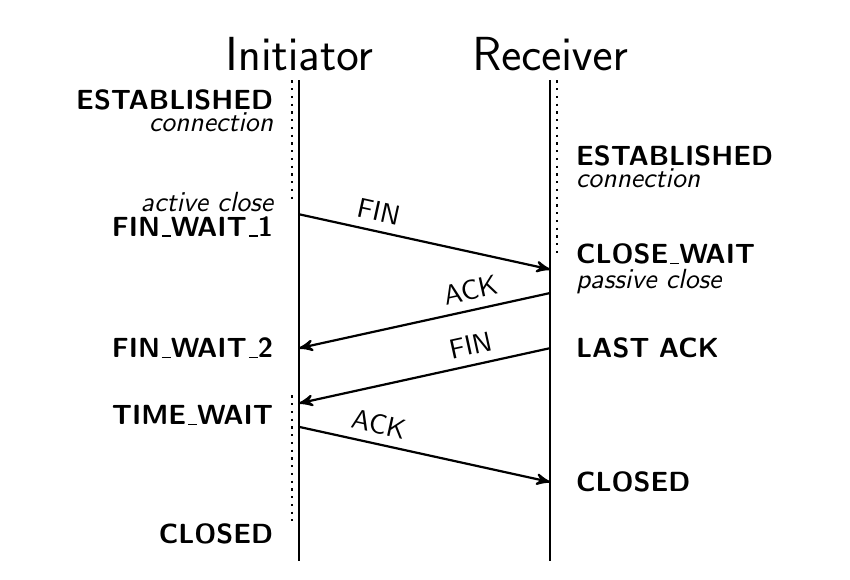
\begin{tikzpicture}[font=\sffamily,>=stealth',thick,
			commentl/.style={text width=3cm, align=right},
			commentr/.style={commentl, align=left},]
		\node[] (init) {\LARGE Initiator};
		\node[right=1cm of init] (recv) {\LARGE Receiver};


		\draw[->] ([yshift=-1.7cm]init.south) coordinate (fin1o) -- ([yshift=-.7cm]fin1o-|recv) coordinate (fin1e) node[pos=.3, above, sloped] {FIN};

		\draw[->] ([yshift=-.3cm]fin1e) coordinate (ack1o) -- ([yshift=-.7cm]ack1o-|init) coordinate (ack1e) node[pos=.3, above, sloped] {ACK};

		\draw[->] (ack1e-|recv) coordinate (fin2o) -- ([yshift=-.7cm]fin2o-|init) coordinate (fin2e) node[pos=.3, above, sloped] {FIN};

		\draw[->] ([yshift=-.3cm]fin2e) coordinate (ack2o) -- ([yshift=-.7cm]ack2o-|recv) coordinate (ack2e) node[pos=.3, above, sloped] {ACK};

		\draw[thick, shorten >=-1cm] (init) -- (init|-ack2e);
		\draw[thick, shorten >=-1cm] (recv) -- (recv|-ack2e);

		\draw[dotted] (recv.285)--([yshift=2mm]recv.285|-fin1e) coordinate[pos=.5] (aux1);

		\draw[dotted] (init.255)--([yshift=2mm]init.255|-fin1o);

		\draw[dotted] ([yshift=1mm]init.255|-fin2e) --([yshift=-5mm]init.255|-ack2e) coordinate (aux2);

		\node[commentr, right =2mm of ack2e] {\textbf{CLOSED}};
		\node[commentr, right =2mm of fin2o] {\textbf{LAST ACK}};
		\node[below left = 0mm and 2mm of init.south, commentl]{\textbf{ESTABLISHED}\\[-1.5mm]{\itshape connection}};
		\node[left = 2mm of fin1o.west, commentl]{{\itshape active close}\\[-1mm]\textbf{FIN\_WAIT\_1}};
		\node[left = 2mm of ack1e.west, commentl]{\textbf{FIN\_WAIT\_2}};
		\node[below left = -1mm and 2mm of fin2e.west, commentl]{\textbf{TIME\_WAIT}};
		\node[below left = -1mm and 2mm of aux2-|init, commentl]{\textbf{CLOSED}};

		\node[right = 2mm of recv|-aux1, commentr]{\textbf{ESTABLISHED}\\[-1.5mm]{\itshape connection}};
		\node[right = 2mm of fin1e.west, commentr]{\textbf{CLOSE\_WAIT}\\[-1mm]{\itshape passive close}};
	\end{tikzpicture}
\end{center}

一个普通TCP连接的建立与终止。通常,由客户端负责发起一个三次握手过程。在该过程中,客户端与服务器利用SYN报文段交换彼此的初始序列号(包括客户端的初始序列号和服
务器的初始序列号)。在通信双方都发送了一个 FIN数据包并收到来自对方的相应的确认数据包后,该连接终止

通过发送上述3个报文段就能够完成一个 TCP连接的建立。它们也常称作三次握手。三次握手的目的不仅在于让通信双方了解一个连接正在建立,还在于利用数据包的选项来承
载特殊的信息,交换初始序列号(Initial Sequence Number, ISN)。

发送首个 SYN 的一方被认为是主动地打开一个连接。如上文所述,它通常是一个客户端。连接的另一方会接收这个SYN,并发送下一个SYN,因此它是被动地打开一个连接。
通常,这一方称为服务器。(13.2.2 节将会介绍一种客户端与服务器同时打开一个连接的情况。这种情况可以作为上文所介绍内容的补充,但非常少见。)

\begin{tcolorbox}[title = {注意}]
    TCP的SYN段也能够承载应用数据。由于伯克利的套接字 API 不支持这种方式,因此它也很少为人所用。
\end{tcolorbox}

图13-1还描绘了一个 TCP连接是怎样关闭的(也称 清除或终止)。连接的任何一方都能够发起一个关闭操作。此外,该过程还支持双方同时关闭连接的操作,但这种情况非常少
见。在传统的情况下,负责发起关闭连接的通常是客户端(如图13-1所示)。然而,一些服务器(例如Web 服务器)在对请求做出响应之后也会发起一个关闭操作。通常一个关闭操作
是由应用程序提出关闭连接的请求而引发的(例如使用系统调用\verb|close()|)。TCP 协议规定通过发送一个 FIN段(即FIN 位字段置位的TCP 报文段)来发起关闭操作。只有当连接双方都
完成关闭操作后,才构成一个完整关闭:
\begin{enumerate}
	\item 连接的主动关闭者发送一个 FIN 段指明接收者希望看到的自己当前的序列号(K,如图 13-1所示)。FIN 段还包含了一个ACK 段用于确认对方最近一次发来的数据(图13-1中标记为L)。
	\item 连接的被动关闭者将K的数位加1作次响应的ACK 位,以表明它已经成功接收到主动关闭者发送的FIN。此时,上层的应用程序会被告知连接的另一端已经提出了关闭的请求。通常,这将导致应用程序发起自己的关闭操作。接着,被动关闭者将身份转变为主动关闭者,并发送自己的FIN。该报文段的序列号为L。
	\item 为了完成连接的关闭,最后发送的报文段还包含一个 ACK用于确认上一个FIN。值得注意的是,如果出现 FIN 丢失的情况,那么发送方将重新传输直到接收到一个ACK 确认为止。
\end{enumerate}

综上所述,建立一个 TCP 连接需要3个报文段,而关闭一个 TCP 连接需要4个报文段。TCP协议还支持连接处于半开启状态(参见13.6.3节),但这种情况并不常见。存在上述半
开启状态的原因在于 TCP的通信模型是双向的。这也意味着在两个方向中可能会出现只有一个方向正在进行数据传输的情况。TCP 的半关闭操作是指仅关闭数据流的一个传输方向,
而两个半关闭操作合在一起就能够关闭整个连接。因此TCP协议规定通信的任何一方在完成数据发送任务后都能够发送一个 FIN。当通信的另一方接收到这个 FIN 时,就会告知应用
程序对方已经终止了对应方向的数据传输。由此可见,当程序发布关闭操作请求后,通信双方往往通过发送 FIN段来关闭双向的数据传输。

如上文所述,7个报文段是每一个 TCP 连接在正常建立与关闭时的基本开销(下文还会介绍一些突然关闭 TCP连接的方式)。因此当只需要交换少量的数据时,一些应用程序更愿
意选择在发送与接收数据之前不需要建立连接的UDP 协议。然而,这些应用程序也会面对由此引入的错误修复、拥塞管理以及流量控制等诸多问题。
\subsection{TCP半关闭}
如前文所述,TCP 支持半关闭操作。虽然一些应用需要此项功能,但它并不常见。为了实现这一特性,API 必须为应用程序提供一种基本的表达方式。例如,应用程序表明“我
已经完成了数据的发送工作,并发送一个 FIN 给对方,但是我仍然希望接收来自对方的数据直到它发送一个 FIN给我”。伯克利套接字的API 提供了半关闭操作。应用程序只需要调用
shutdown() 函数来代替基本的\verb|close()|函数,就能实现上述操作。然而,绝大部分应用程序仍然会调用 \verb|close()|函数来同时关闭一条连接的两个传输方向。图13-2展示了一个正在使用的
半关闭示例。图中左侧的客户端负责发起半关闭操作,然而在实际应用中,通信的任何一方都能完成这项工作。

首先发送的两个报文段与TCP正常关闭完全相同:初始者发送的FIN,接着是接收者回应该FIN的ACK。由于接收到半关闭的一方仍能够发送数据,因此图13-2 中的后续操作与
图13-1不同。虽然图13-2 在ACK之后只描述了一个数据段的传输过程,但实际应用时可以传输任意数址的数据段(第1S 章将会详细地讨论数据段的交换与确认细节)。当接收半关
闭的一方完成数据发送后,它将会发送一个FIN半关闭本方的连接,同时向发起半关闭的应用程序签出一个文件尾指示。当第2个FIN 被确认之后,整个连接完全关闭。

\subsection{同时打开与关闭}
虽然两个应用程序同时主动打开连接看似不大可能,但是在特定安排的情况下是有可能实现的。通信双方在接收到来自对方的SYN之前必须先发送一个 SYN;两个 SYN必须经
过网络送达对方。该场景还要求通信双方都拥有一个 IP 地址与端口号,并且将其告知对方。上述情况十分少见(第7章介绍的防火墙“打孔”技术除外),一旦发生,可称其同时打开。

例如,主机A的一个应用程序通过本地的7777端口向主机B 的8888端口发送一个主动打开请求,与此同时主机B 的一个应用程序也通过本地的8888端口向主机A的7777端
口提出一个主动打开请求,此时就会发生一个同时打开的情况。这种情况不同于主机A的一个客户端连接主机B的一个服务器,而同时又有主机B的一个客户端连接主机A的一个服
务器的情况。在这种情况下,服务器始终是连接的被动打开者而非主动打开者,而各自的客户端也会选择不同的端口号。因此,它们可以被区分为两个不同的 TCP 连接。图13-3显示
了在一个同时打开过程中报文段的交换情况。

一个同时打开过程需要交换4个报文段,比普通的三次握手增加了一个。由于通信双方都扮演了客户端与服务器的角色,因此不能够将任何一方称作客户端或服务器。同时关闭并
没有太大区别。如前文所述,通信一方(通常是客户端,但不一定总是)提出主动关闭请求,并发送首个 FIN。在同时关闭中,通信双方都会完成上述工作。图13-4显示了在一个同时关
闭中需要交换的报文段。

在同时打开中交换的报文段。与正常的连接建立过程相比,需要增加一个报文段。数据包的SYN 位将置位直到接收到一个ACK 数据包止

在同时关闭中交换的报文段。与正常关闭相似,只是报文段的顺序是交叉的

同时关闭需要交换与正常关闭相同数量的报文段。两者真正的区别在于报文段序列是交又的还是顺序的。下文将会介绍 TCP 实现中同时打开与同时关闭操作使用特殊状态这一不
常见的方法。
\subsection{初始序列号} \label{ssec:initseq}
当一个连接打开时,任何拥有合适的IP地址、端口号、符合逻辑的序列号(即在窗口中)以及正确校验和的报文段都将被对方接收。然而,这也引入了另一个问题。在一个连接
中,TCP 报文段在经过网络路由后可能会存在延迟抵达与排序混乱的情况。为了解决这一问题,需要仔细选择初始序列号。本节将详细介绍这一过程。

在发送用于建立连接的SYN之前,通信双方会选择一个初始序列号。初始序列号会随时间而改变,因此每一个连接都拥有不同的初始序列号。[\href{https://datatracker.ietf.org/doc/html/rfc793#section-3.3}{RFC793}] 指出初始序列号可被视
为一个32 位的计数器。该计数器的数值每4微秒加1。此举的目的在于为一个连接的报文段安排序列号,以防止出现与其他连接的序列号重叠的情况。尤其对于同一连接的两个不同实
例而言,新的序列号也不能出现重叠的情况。

由于一个TCP连接是被一对端点所唯一标识的,其中包括由2个IP地址与2个端口号构成的4元组,因此即便是同一个连接也会出现不同的实例。如果连接由于某个报文段的长
时间延迟而被关闭,然后又以相同的4元组被重新打开,那么可以相信延迟的报文段又会被视为有效数据重新进入新连接的数据流中。上述情况会令人十分烦恼。通过采取一些步骤来
避免连接实例间的序列号重叠问题,能够将风险降至最低。即便如此,一个对数据完整性有较高要求的应用程序也可以在应用层利用 CRC 或校验和保证所需数据在传输过程中没有出
现任何错误。在任何情况下这都是一种很好的方法,并已普遍用于大文件的传输。

如前文所述,一个TCP报文段只有同时具备连接的4元组与当前活动窗口的序列号,才会在通信过程中被对方认为是正确的。然而,这也从另一个侧面反映了 TCP 的脆弱性:如
果选择合适的序列号、IP地址以及端口号,那么任何人都能伪造出一个TCP报文段,从而打断 TCP 的正常连接[\href{https://datatracker.ietf.org/doc/html/rfc5961#section-5}{RFC5961}]。
一种抵御上述行为的方法是使初始序列号(或者临时端口号TRFC6056])变得相对难以被猜出,而另一种方法则是加密(参见第18章)。

现代系统通常采用半随机的方法选择初始序列号。证书报告CA-2001-09 [CERTISN] 讨论了这一方法的具体实现细节。\emph{\color{red}Linux 系统采用一个相对复杂的过程来选择
它的初始序列号\footnotemark。它采用基于时钟的方案,并且针对每一个连接为时钟设置随机的偏移量。随机偏移量是在连接标识(即4元组)的基础上利用加密散列函数得到的。散列函数的输入
每隔5分钟就会改变一次。在32位的初始序列号中,最高的8位是一个保密的序列号,而剩余的各位则由散列函数生成。上述方法所生成的序列号很难被猜出,但依然会随着时间而逐
步增加。}据报告显示,Windows 系统使用了一种基于 RC4[S94]的类似方案。
\footnotetext{详细代码见\href{https://elixir.bootlin.com/linux/v4.4.302/source/net/core/secure_seq.c\#L89}{linux isn generate}, 
linux 4.4中使用的散列函数为\href{https://elixir.bootlin.com/linux/v4.4.302/source/lib/md5.c\#L13}{md5}}
\subsection{例子}
前文介绍了一个 TCP 连接的建立和退出过程,本节将从数据包(分组)的角度进一步介绍相关细节。为此我们尝试对邻近的Web 服务器进行 TCP连接。该主机的IPv4地址为
\verb|10.0.0.2|,而客户端则采用了基于 Windows 的\verb|telnet| 应用。

\iffalse
	C:\> telnet \verb|10.0.0.2| 80
	Welcome to
	Microsoft telnet Client
	Escape Character is
	' CTRI+]'
	wait about
	4.4 seconds
	Microsoft telnet> quit
\fi

\verb|telnet|命令是建立在 TCP 连接的基础上的。在上述例子中,该TCP 连接必须与服务器的IPv4 地址\verb|10.0.0.2| 以及http或 Web 服务的端口号(80端口)相关联。当 \verb|telnet| 应用程序连接
23(\verb|telnet| 协议的众所周知端口\href{https://www.rfc-editor.org/rfc/rfc0854}{[RFC0854]})以外的端口,它将不能用于应用协议。它仅仅将自己的字节输入拷贝至TCP连接中,反之亦然。当一个 Web 服务器接收到进入的连接请求
时,它首先需要等待对 web 页面的请求。在这种情况下,我们不能提供这样的请求,因此服务器不会产生任何数据。这些均符合我们的期望,因为我们只对连接建立与终止过程中的数
据包交换感兴趣。图13-5展示了 Wireshark 软件对该命令所产生的报文段的输出结果。

如图13-5所示,客户端发送的SYN报文段所包含的初始序列号为 685506836,通告窗口为65535。该报文段还包含了若干其他选项。13.3节将详细地讨论这些选项。第二个报文
段既包含了服务器的SYN 还包含了对客户端请求的ACK 确认。它的序列号(服务器的初始序列号)为1479690171,ACK 号为 685506837。ACK 号仅比客户端的初始序列号大1,说
明服务器已经成功接收到了客户端的初始序列号。该报文段同样也包含了一个通告窗口以表明服务器愿意接收64240个字节。第三个数据包将最终完成三次握手,它的ACK为
1479690172。ACK 号是不断累积的,并且总是表明ACK发送者希望接收到的下一个序列号(而不是它上一个接收到的序列号)。

在4.4秒暂停之后,\verb|telnet| 应用程序被要求关闭连接。这使得客户端发送第4个报文段FIN。FIN 的序列号为 685506837,并由第5个报文段确认(ACK 号为 685506838)。稍后,
服务器会发送自己的FIN,对应的序列号为1479690172。该报文段对客户端的FIN 进行了再次确认。值得注意的是,该报文段的PSH位被置位。虽然这样并不会对连接的关闭过程
产生实质影响,但通常用于说明服务器将不会再发送任何数据。最后一个报文段用于对服务器的 FIN 进行确认,ACK 号为 1479690173。

\begin{figure}[ht]
	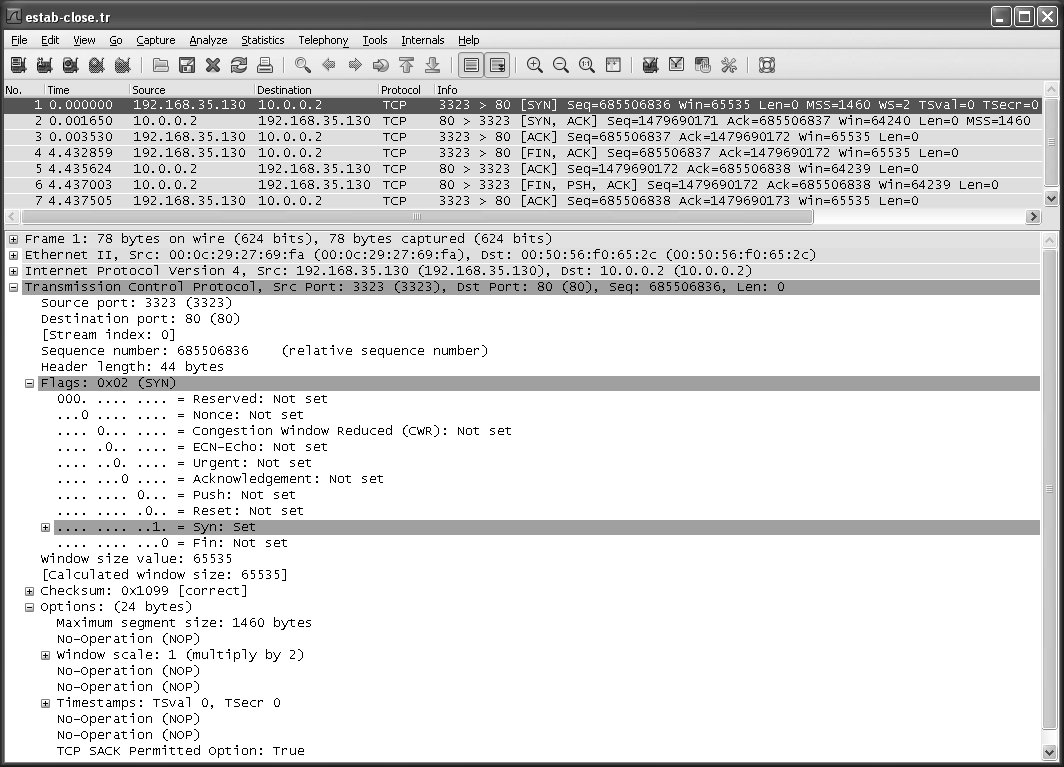
\includegraphics[width=1.0\textwidth]{imgs/13/13-5.png}
	\caption{在主机192.168.35.130与10.0.0.2之间建立一条 TCP 连接,并在不发送任何数据的情况下关闭。PSH(推送)位说明第6个报文段正在发送所有来自缓存的数据(而缓存为空)}
\end{figure}

注意 \href{https://www.rfc-editor.org/rfc/rfc1025}{[RFC1025]} 将拥有最多特性(例如标记与选项)的报文段称力“神风”(kamikaze)数据包。其他生动的术语还包括“丑恶报文”、“圣诞树数据包”、“灯测试”报文段。

从图13-5中我们还会发现SYN报文段包含了一个或多个选项。这些选项需要占用 TCP头部额外的空间。例如,第一个 TCP 头部的长度为44字节,比最小的长度长24字节。TCP
也提供了若干选项,下文将详细介绍当一个连接无法建立时如何使用这些选项。
\subsection{连接建立超时}
本节的若干实例将会展示连接不能建立的情况。一种显而易见的情况是服务器关闭。为了模拟这种情况,我们将 \verb|telnet|命令发送给一个处于同一子网的不存在的主机。在不修改
ARP 表的情况下,上述做法会使客户端收到一个“无法到达主机”的错误消息后退出。由于没有接收到针对之前发送的ARP 请求而返回的ARP 响应(参见第4章),因此会产生“无
法到达主机”的消息。如果我们能事先在 ARP 表中为这个不存在的主机添加一条记录,那么系统就不需要发送 ARP 请求,而会马上根据 TCPAIP 协议尝试与这个不存在的主机建立联
系。相关的命令如下:

\iffalse
	Linux# arp -s 192.168.10.180 00:00:1a: 1b: 10:1đ
	Linux8 date; \verb|telnet| 192.168.10.180 80; date
	7 21:16:34 PDT 2009
	Trying 192.168.10.180...
	to address 192.168.10.180:
	Connection timed out
	7 21:19:43 PDT 2009
\fi

上述例子选择的 MAC地址 00:00:1a:1b:1c:1d 不能与局域网中其他主机的MAC冲突,除此之外并无特别。超时发生在发送初始命令后的3.2分钟。由于没有主机响应,例子中所
有的报文段都是由客户端产生的。清单 13-1 显示了使用 \verb|Wireshark| 软件在摘要模式下获得的输出结果。

有趣的是这些输出结果显示了客户端 TCP 为了建立连接频繁地发送 SYN 报文段。在首个报文段发送后仅3秒第二个报文段就被发送出去,第三个报文段则是这之后的6秒,而第
四个报文段则在第三个报文段发送12秒以后被发送出去,以此类推。这一行为被称作指数回退。在讨论以太网CSMA/CD 介质访问控制协议时(参见第3章)我们也曾见过这样的行
为。然而,这两种指数回退也略有不同。此处的每一次回退数值都是前一次数值的两倍,而在以太网中最大的回退数值是上一次的两倍,实际的回退数值则需要随机选取。

一些系统可以配置发送初始SYN 的次数,但通常选择一个相对较小的数值5。在Linux系统中,系统配置变量 \verb|net.ipv4.tcp_syn_retries| 表示了在一次主动打开申请中尝试重新发送
SYN 报文段的最大次数。相应地,变量\verb|net.ipv4.tcp_synack_retries| 表示在响应对方的一个主动打开请求时尝试重新发送SYN+ACK报文段的最大次数。此外,它能够在设定Linux专
有的TCP\_SYNCNT套接字选项的基础上用于个人连接。正如上面所介绍的,默认的数值为重试5次。两次重新传输之间的指数回退时间是 TCP拥塞管理响应的一部分。当我们讨论
Kam 算法时再仔细研究。
\subsection{连接与转换器}
在第7章,我们已经讨论了一些协议(比如 TCP 和 UDP)如何利用传统的NAT 转换地址与端口号。我们还讨论了 IP 数据包如何在IPv6 与IPv4 两个版本间进行转换。当TCP使
用NAT时,伪头部的校验和通常需要调整(使用校验和中立地址修改器的情况除外)。其他协议也使用伪头部校验和,因为计算包含了与传输层、网络层相关的信息。

当一个 TCP连接首次被建立时,NAT 能够根据报文段的SYN位探明这一事实。同样可以通过检查SYN+ACK报文段与ACK报文段所包含的序列号来判断一个连接是否已经
完全建立。上述方法还适用于连接的终止。通过在 NAT 中实现一部分TCP 状态机(参5IRFC6146]的3.5.2.1 节与3.5.2.2 节)能够跟踪连接,包括当前状态、各方向的序列号以及
相关的 ACK 号。这种状态跟踪是典型的 NAT 实现方法。

当NAT 扮演编辑者的角色并且向传输协议的数据负载中写人内容时,就会涉及一些更复杂的问题。对于 TCP 而言,它将会包括在数据流中添加与删除数据,并由此影响序列号
(与报文段)的长度。此举会影响到校验和,但也会影响数据的顺序。如果利用NAT在数找流中插人或删除数据,这些数值都要做出适当调整。如果 NAT 的状态与终端主机的状态不
同步,连接就无法正确进行下去。因此,上述做法会带来一定的脆弱性。

\section{TCP选项} \label{tcpOpt}
如图12-3所示,TCP 头部包含了多个选项。选项列表结束(End of Option List, EOL)无操作(No Operation, NOP)以及最大段大小(Maximum Segment Size, MSS)是定义于原
始TCP规范中的选项。自那时起,又有若干选项被定义。整个选项列表是由互联网编号分配机构(IANA)维护的[TPARAMS]。表13-1列举了一些目前有趣的选项(即,符合RFC
标准化描述的选项)。

\iffalse
	0

	EOL
	\href{https://www.rfc-editor.org/rfc/rfc0793}{[RFC0793]}
	选项列表结束


	NOP
	(RFC0793]
	无操作(用于填充)


	MSS
	\href{https://www.rfc-editor.org/rfc/rfc0793}{[RFC0793]}
	最大段大小


	WSOPT
	\href{https://www.rfc-editor.org/rfc/rfc01323}{[RFC01323]}
	窗口缩放因子(窗口左移量)


	SACK-Permitted
	\href{https://www.rfc-editor.org/rfc/rfc02018}{[RFC02018]}
	发送者支持 SACK 选项

	可变
	SACK
	\href{https://www.rfc-editor.org/rfc/rfc02018}{[RFC02018]}
	SACK 阻塞(接收到乱序数据)

	10
	TSOPT
	\href{https://www.rfc-editor.org/rfc/rfc01323}{[RFC01323]}
	时间戳选项
	28
	4
	UTO
	\href{https://www.rfc-editor.org/rfc/rfc05482}{[RFC05482]}
	用户超时(一段空闲时间后的终止)
	29
	可变
	TCP-AO
	[RFCO5925]
	认证选项(使用多种算法)
	253
	可变
	Experimental
	\href{https://www.rfc-editor.org/rfc/rfc04727}{[RFC04727]}
	保留供实验所用
	254
	可变
	Experimental
		\href{https://www.rfc-editor.org/rfc/rfc04727}{[RFC04727]}
	保留供实验所用
\fi

每一个选项的头一个字节为“种类”(kind),指明了该选项的类型。根据\href{https://www.rfc-editor.org/rfc/rfc1122}{[RFC1122]},不能被理解的选项会被简单地忽略掉。种类值为0或1的选项仅占用一个字节。其他的选项会
根据种类来确定自身的字节数len。选项的总长度包括了种类与len 个字节。设置 NOP 选项的目的是允许发送者在必要的时候用多个4字节组填充某个字段。需要记住的是 TCP 头部
的长度应该是32比特的倍数,因为TCP 头部长度字段是以此为单位的。EOL 指出了选项列表的结尾,说明无需对选项列表再进行处理。在下文中,我们将详细地探究其他选项。

\subsection{最大段大小选项}
最大段大小是指 TCP 协议所允许的从对方接收到的最大报文段,因此这也是通信对方在发送数据时能够使用的最大报文段。根据[RFCO879],最大段大小只记录 TCP 数据的字
节数而不包括其他相关的TCP 与IP头部。当建立一条TCP 连接时,通信的每一方都要在SYN报文段的MSS 选项中说明自己允许的最大段大小。这16位的选项能够说明最大段大
小的数值。在没有事先指明的情况下,最大段大小的歌认数位为596字节。前文留介绍过,任何主机都应该能够处理至少576字节的IPv4数据报。如果按照最小的 IPv4 与 TCP头
部计算,TCP 协议要求在每次发送时的最大段大小为536字节,这样就正好能够组成一个$576(20+20+536= 576)$字节的IPv4数据报。

图13-5中,最大段大小的数值均为1460。这是IPv4 协议中的典型值,因此IPv4数据数据报的大小也相应增加 40 个字节(总共1500字节,以太网中最大传输单元与互联网路径最大
传输单元的典型数值):20字节的 TCP 头部加20字节的IP 头部。当使用 IPv6协议时,最大段大小通常为1440字节。由于IPv6 的头部比IPv4多20个字节,因此最大段大小的数值相
应减少20字节。在\href{https://www.rfc-editor.org/rfc/rfc2675}{[RFC2675]} 中65535 是一个特数值,与IPv6 超长数据报一起用来指定一个表示无限大的有效最大段大小值。在这种情况下,发送方的最大段大小等于路径MTU
的数值减去60字节(40字节用于IPv6头部,20字节用于 TCP 头部)。值得注意的是,最大段大小并不是TCP 通信双方的协商结果,而是一个限定的数值。当通信的一方将自己的最
大段大小选项发送给对方时,它已表明自己不愿意在整个连接过程中接收任何大于该尺寸的报文段。

\subsection{选择确认选项}
第12 章介绍了滑动窗口的概念,并描述了TCP 协议是如何管理序列号与确认的。由于采用累积 ACK确认,TCP不能正确地确认之前已经接收的数据。由于接收的数据是无序的,
所以接收到数据的序列号也是不连续的。在这种情况下,TCP 接收方的数据队列中会出现空洞的情况。因此在提供字节流传输服务时,TCP接收方需要防止应用程序使用超出空洞的
数据。

如果 TCP 发送方能够了解接收方当前的空洞(以及在序列空间中超出空洞的乱序数据块),它就能在报文段丢失或被接收方遗漏时更好地进行重传工作。根据\href{https://www.rfc-editor.org/rfc/rfc2018}{[RFC2018]}与
\href{https://www.rfc-editor.org/rfc/rfc2883}{[RFC2883]},TCP“选择确认”(SACK)选项提供了上述功能。如果 TCP接收方能够提供选择确认信息,并且发送方能够合理有效地利用这些信息,那么上述方案将会十分高效。

通过接收SYN(或者 SYN +ACK)报文段中的“允许选择确认”选项,TCP通信方会了解到自身具有了发布SACK 信息的能力。当接收到乱序的数据时,它就能提供一个 SACK
选项来描述这些乱序的数据,从而帮助对方有效地进行重传。SACK 信息保存于SACK 选项中,包含了接收方已经成功接收的数据块的序列号范围。每一个范围被称作一个SACK块,
由一对32 位的序列号表示。因此,一个 SACK 选项包含了n个 SACK块,长度为(8n +2)个字节。增加的2个字节用于保存SACK 选项的种类与长度。

由于TCP 头部选项的空间是有限的,因此一个报文段中发送的最大SACK 块数目为3(假设使用了时间戳选项。根据13.3.4节的介绍,这是现代 TCP 实现中的典型情况)。虽然只
有SYN报文段才能包含“允许选择确认”选项,但是只要发送方已经发送了该选项,SACK块就能够通过任何报文段发送出去。由于选择确认的操作相对于 TCP的错误和拥塞控制的
操作而言更简单,本书将在第14 章与第16章再介绍相关的细节。
\subsection{窗口缩放选项}
根据 \href{https://www.rfc-editor.org/rfc/rfc1323}{[RFC1323]},窗口缩放选项(表示 WSCALE 或 WSOPT) 能够有效地将 TCP 窗口广告字段的范围从16 位增加至30位。TCP 头部不需要改变窗口通告字段的大小,仍然维持
16位的数值。同时,使用另一个选项作为这16位数值的比例因子。该比例因子能够使窗口字段值有效地左移。这样事实上将窗口数值 大至原先的$2^n$倍,其中$n$为比例因子。一个字
节的移动可以用0至14(包含14)来计数。计数。的移动表示没有任何比例。最大的比例数值是14,它能够提供一个最大为1 073 725440字节$(65535 ×2^(14))$的窗口。该数值接
近$1073 741 823(2^(30)-1)$,正好1GB。因此,TCP使用一个32位的值来维护这个“真实”的窗口大小。

该选项只能出现于一个SYN报文段中,因此当连接建立以后比例因子是与方向绑定的。为了保证窗口调整,通信双方都需要在SYN报文段中包含该选项。主动打开连接的一方利
用自己的SYN中发送该选项,但被动打开连接的一方只能在接收到的SYN 中指出该选项时才能发送。每个方向的比例因子可各不相同。如果主动打开连接的一方发送了一个非0的比
例因子但却没有接收到来自对方的窗口缩放选项,它会将自己发送与接收的比例因子数值都设为0。这样使得系统不需要理解这些系统间的选项互操作。

假设我们正在使用窗口缩放选项,发送出去的窗口移动数值S,而接收到的窗口移动数值为R。这样,我们从对方接收到每一个16位的广告窗口都需要左移R位才能获得真实
窗口大小。每次向对方发送窗口通告时,都会将32位的窗口大小向右移动S位,然后将16位的数值填充到 TCP头部。

窗口的移动数值是由 TCP通信方根据接收缓存的大小自动选取的。缓存的大小是由系统设定的,但是应用程序通常都具有改变其大小的能力。当TCP协议被用于在大带宽、高
延迟网络(即,往返时间与带宽都相对较大的网络)上提供海量数据传输服务时,窗口缩放选项就非常有意义。因此,第16章将会进一步讨论该选项的重要性与使用方法。

\subsection{时间戳选项与防回绕序列号}
时间戳选项(记作 TSOPT 或TSopt)要求发送方在每一个报文段中添加2个4字节的时间戳数值。接收方将会在确认中反映这些数值,允许发送方针对每一个接收到的ACK 估
算 TCP连接的往返时间(由于 TCP 协议经常利用一个ACK 来确认多个报文段,此处必须指出是“每个接收到的ACK”而不是“每个报文段”。本书第15 章将会详细地讨论这一问
题)。当使用时间戳选项时,发送方将一个32位的数值填充到时间戳数值字段(称作 TSV 或TSval)作时间戳选项的第一个部分;而接收方则将收到的时间戳数值原封不动地填充至第
二部分的时间截回显重试字段(称作 TSBR 或 TSecr)。由于包含了时间截选项,TCP 头部的长度将会增长 10字节(8字节用于保存2个时间戳数值,而另2个数值则用于指明选项的数
值与长度)。

时间戳是一个单调增加的数值。由于接收者只会对它接收到的信息做出响应,所以它并不关心时间戳单元或数值到底是什么。该选项并不要求在两台主机之间进行任何形式的时钟
同步。\href{https://www.rfc-editor.org/rfc/rfc1323}{[RFC1323]} 推荐发送者每秒钟至少将时间戳数值加1。图13-6显示了通过 Wireshark软件获得的时间戳选项。

上述例子中,通信双方都产生并回应了对方的时间戳。第一个报文段(客户端的SYN)使用一三个初始的时间戳数位 81813090。该数值被域充在时间破数位子段中。由于容户端
并不知道服务器的时间戳数值,所以该报文段的第二部分时间戳回显重试字段的数值为0。

一个使用了时间戳、窗口缩放以及最大段大小选项的TCP连接。TCP头部长度为44字节。
初始SYN(第1个数据包)的时间戳数值为81813090。图中高亮标记的第二个数据包将这一数值作为响应返回给主动打开连接的一方,同时包含了自己的数值349742014

估算一条TCP连接的往返时间主要是为了设置重传超时。重传超时用于告知TCP通信方何时应该重新发送可能已经丢失的报文段。第12章已经讨论了在一些往返时间函数
的基础上设置此项超时的必要性。借助时间戳选项,我们能够获得往返时间相对精确的测量结果。在使用时间戳选项之前,大多 TCP通信会针对每个窗口的数据抽取一个往返时间
样本。时间戳选项使我们获得了更多的样本,从而提升了精确估算往返时间的能力(参见[RFC13231 与 \href{https://www.rfc-editor.org/rfc/rfc6298}{[RFC6298]})。

由于时间戳选项与重传计时器的设置紧密相关,我们将在第14 章讨论重传问题时详细地介绍时间戳选项的这一用途。“这一用途”是为了强调虽然时间戳选项允许更高频率的往
返时间样本,但它也为接收者提供了避免接收旧报文段与判断报文段正确性的方法。这被称作防回绕序列号(Protection Against Wrapped Sequence numbers, PAWS),它与时间戳选项
一起记录于\href{https://www.rfc-editor.org/rfc/rfc1323}{[RFC1323]}中。现在,我们要继续探究一下它是如何工作的。

假设一个 TCP 连接使用了窗口缩放选项,并将其设置为可能最大的窗口,大约1GB。再假设使用了时间戳选项,并且发送者针对发送的每个窗口分配的时间戳数值都会加1。(这
一假设是保守的。正常情况下时间戳数值的增长速度要远快于此。)表13-2显示了当传输6GB 数据时两个主机之间可能的数据流。为了避免过多的10位数字,我们使用符号G表
示1073 741824 的倍数。我们还再次采用了 tcpdump 中的符号J:K来表示从第J个字节到第K-1个字节的数据。

TCP时间戳选项通过提供一个额外的32位有效序列号空间清除了具有相同序列号的报文段之间的二义性

32位序列号字段在时刻D和时刻E间回绕。假设在时刻B有一个报文段丢失并被亘传。又假设这一丢失的报文段在时刻F重新出现。假设报文段丢失与重新出现的时间差小于
一个报文段在网络中存在的最大时间(称为 MSL,参见13.5.2节),否则当路由器发现TTL期满后就会丢弃该报文段。正如我们之前提到的,旧的报文段重新出现并包含当前正在传输
的序列号的问题只会发生在相对高速的连接中。

由表13-2可以看出,使用时间戳选项能够有效地防止上述问题。接收者可以将时间言看作一个32位的扩展序列号。丢失的报文段会在时刻F重新出现,由于它的时间戳为2,小
于最近的有效时间戳(5或6),因此防回绕序列号算法会将其丢弃。防回绕序列号算法并不要求在发送者与接收者之间有任何形式的时钟同步。接收者所需要的是保证时间戳数值单调
增长,并且每一个窗口的数据至少增加1。

\subsection{用户超时选项}
根据TRFC5482]的描述,用户超时(UTO)选项是一个相对较新的TCP 的功能。用户超时数值(也被称力 USER\_TIMEOUT) 指明了 TCP 发送者在确认对方未能成功接收数据之前
愿意等待该数据 ACK 确认的时间。根据\href{https://www.rfc-editor.org/rfc/rfc0793}{[RFC0793]},USER\_TIMEOUT 是 TCP 协议本地配置的一个参数。用户超时选项允许TCP 通信方将自己的USER\_TIMEOUT 数值告知连接的
对方。这样就方便了 TCP 接收方调整自己的行为(例如,在终止连接之前容忍一段较长时间的连接中断)。NAT设备也能够解释这些信息以帮助设置它们的连接活动计时器。

用户超时选项的数值是建议性的,因为即便连接的一端希望使用一个大的或小的数信也不意味着另一端就必须遵从。[RFCI122]提炼了 USER\_TINEOUT 的定义,并且建议当
TCP 连接达到3次重传阈值时应该通知应用程序(规则1),而当超时大于100秒时应该关闭连接(规则2)。某些实现会提供 API 函数来修改规则1与规则2。由于长的用户超时设置
会导致资源耗尽,而短的用户超时设置可能会导致一些连接过早地断开(例如,拒绝服务攻击),因此需要为用户超时选项的可能数值设置上下边界。设置 USER\_TIMEOUT 的具体方
法如下:
USER\_TIMEOUT = min(U\_LIMIT, max (ADV\_UTO, REMOTE\_UTO, L\_LIMIT) )

其中 ADV\_UTO 是本端告知远端通信方的用户超时选项数值,而 \_UTO是远端通信方告知的用户超时选项数值,U\_LIMIT 是本地系统对用户超时选项设定的数值上边界
,而L\_LIMIT 则是下边界。值得注意的是上式并不能保证同一连接的两端会获得相同的用户超时数值。在任何情况下,L\_LIMIT 的数值必须大于对应连接的重传超时数值(参见第1
章)。L\_LINIT的数值一般推荐设为100 秒,这样可以保持与『RFC1122]相兼容。

建立连接的 SYN报文段、首个非SYN报文段以及 USER\_TIMEOUT 的数值发生任何改变的报文段,都会包含用户超时选项。该选项的数值由一个 15位的数值部分与一个1位的
单位部分构成。单位部分用于说明数值的计量单位是分钟(1)还是秒(0)。UTO 作为一个相对较新的选项还没有得到广泛使用。

\subsection{认证选项}
TCP设置了一个选项用于增强连接的安全性。设计该选项的目的在于增强与替换较早的TCP-MDS 机制 \href{https://www.rfc-editor.org/rfc/rfc2385}{[RFC2385]}。这一选项被称作TCP 认证选项 (TCP Authentication Option,
TCP-AO)\href{https://www.rfc-editor.org/rfc/rfc5925}{[RFC5925]},它使用了一种加密散列算法(参见第18章)以及 TCP连接双方共同维护的一个秘密值来认证每一个报文段。TCP 认证选项不仅提供各种加密算法,还使用“带
内”信令来确认密钥是否改变,因此它与TCP-MDS 相比有很大的提高。然而,TCP 认证选项没有提供一个全面密钥管理方案。也就是说,通信双方不得不采用一种方法在TCP认证
选项运行之前建立出一套共享密钥。

当发送数据时,TCP 会根据共享的密钥生成一个通信密钥,并根据一个特的加密算法[RFCS926] 计算散列值。接收者装配有相同的密钥,同样也能够生成通信密钥。借助通信密
钥,接收者可以确认到达的报文段是否在传输过程中被篡改过(有非常高的可能性)。设置该选项是为了针对各种 TCP 欺骗攻击提供强有力的抵御策略(参见13.8节)。然而,由于需
要创建并分发一个共享密钥(这是一个相对新的选项),该选项并没有得到广泛使用。
\section{TCP 的路径最大传输单元发现}
第3章介绍了路径最大传输单元(MTU)的概念。它是指经过两台主机之间路径的所有网络报文段中最大传输单元的最小值。知道路径最大传输单元后能够有助于一些协议(比如
TCP)避免分片。第10章介绍了基于ICMP消息的路径最大传输单元发现(PMTUD)过程是如何实现的,但由于应用程序已经指定了尺寸(即,非传输层协议),UDP协议一般不会
采用上述发现过程获得的数据报大小。TCP 在支持字节流抽象的实现过程中能够决定使用多大的报文段,因此它很大程度上控制了最后生成的IP数据包。

在本节中,我们将会进一步探寻 TCP 是如何使用路径最大传输单元的。我们的讨论内容适用于 TCP/IPv4 与TCP/IPV6。\href{https://www.rfc-editor.org/rfc/rfc1191}{[RFC1191]}与\href{https://www.rfc-editor.org/rfc/rfc1981}{[RFC1981]}能分别提供更多的细节。一种称
作分组层路径最大传输单元发现(Packetization Layer Path MTU Discovery, PLPMTUD)的算法能够避免对ICMP的使用。根据\href{https://www.rfc-editor.org/rfc/rfc4821}{[RFC4821]},该算法也能够被TCP或其他传输协议使
用。我们可以利用 IPv6 协议中 “数据包太大”(Packet Too Big, PTB)的术语来代表 ICMIPv4地址不可达(需要分片)或ICMPv6 数据包太大的消息。

TCP 常规的路径最大传输单元发现过程如下:在一个连接建立时,TCP 使用对外接口的最大传输单元的最小值,或者根据通信对方声明的最大段大小来选择发送方的最大段大小
(SMSS)。路径最大传输单元发现不允许 TCP 发送方有超过另一方所声明的最大段大小的行为。如果对方没有指明最大段大小的数值,发送方将假设采用默认的536字节,但是这种情
况比较少见。如果为每一个目的地保存对应的路径最大传输单元,那么就能方便地对段大小进行选择。值得注意的是,一条连接的两个方向的路径最大传输单元是不同的。

一旦为发送方的最大大小选定了初始值,TCP通过这条连接发送的所有IPv4 数据报都会对 DF位字段进行设置。TCP/IPv6 没有DF 位字段,因此只需要假设所有的数据报都已经
设置了该字段而不必进行实际操作。如果接收到 PTB 消息,TCP 就会减少段的大小,然后用修改过的段大小进行重传。如果在PTB 消息中已包含了下一眺推荐的最大传输单元,段
大小的数值可以设置为下一眺最大传输单元的数值减去 IPv4(或IPv6)与TCP头部的大小。如果下一眺最大传输单元的数值不存在(例如,一个之前的ICMP 错误被返回时会缺乏这一
信息),发现者可能需要尝试多个数值(例如,采用二分搜案法选择一个可用的数值)。这也会影响到 TCP的拥塞控制管理(参见第16 章)。对于分组层路径最大传输单元发现而言,除
了PTB的消息不被使用以外其他情况基本类似。相反,执行路径最大传输单元发现的协议必须能够快速地检测消息丢弃并调整自己的数据报大小。

由于路由是动态变化的,在减少段大小的数值一段时间后需要尝试一个更大的数值(接近初始的发送方最大段大小)。根据\href{https://www.rfc-editor.org/rfc/rfc1191}{[RFC1191]}与\href{https://www.rfc-editor.org/rfc/rfc1981}{[RFC1981]}的指导意见,该时间间隔大约
为10分钟。

在互联网环境中,由于防火墙阻塞 PTB 消息\href{https://www.rfc-editor.org/rfc/rfc2923}{[RFC2923]},路径最大传输单元发现过程会存在一些问题。在各种操作问题中,黑洞问题的情况虽有所好转(在[LS10]中,80\%被调查
的系统都能够正确地处理PTB 消息),但仍悬而未决。在 TCP 实现依靠传输 ICMP 消息来调整它的段大小的情况下,如果 TCP 从未接收到任何ICMP 消息,那么在路径最大传输单元发
现过程中就会造成黑洞问题。这种情况可能由多方面的原因造成,其中包括了防火墙或NAT配置为禁止转发ICMP 消息。其后果在于一旦 TCP使用了更大的数据包将不能被正确处理。
由于只是不能转发大数据包,所以诊断出这一问题是十分困难的。那些较小的数据包(比如用于建立连接的 SYN与SYN +ACK 数据包)是能够成功处理的。一些TCP 实现具有“黑
洞探测”功能。当一个报文段在反复重传数次后,将会尝试发送一个较小的报文段。
\subsection{例子}
当中间路由器的最大传输单元小于任何一个通信端的最大段大小时,TCP 就会执行路径最大传输单元发现过程。为了创造上述条件,本文使用一台路由器(一台本地地址为
\verb|10.0.0.1| 的Linux 主机)通过PPPoE 接口连接DSL 服务提供商。PPPoE 链路使用的最大传输单元为1492字节(以太网的最大传输单元为1500字节,减去 PPPOE协议的6字节负载,再
减去2字节的 PPP 负载。参见第13章)。图13-7显示了上述例子的拓扑结构。

PPPoE 封装使 TCP 连接的路径最大传输单元从1500字节(以太网最大传输单元的典型值)减至
1492字节。为了证明 TCP的路径 MTU 发现功能,此例设置了更小的最大传输单元(288予节)

为了更加明显地看出这一行为,将 PPPOE 链路最大传输单元的数值以1492减少至288字节。通过在图13-7的GW 主机上执行下面的命令来完成这项工作:

此外,还需要告知客户端(图13-7中的c)系统允许的最小报文段大小:

如果不执行第2步操作,Linux 系统会将路径最大传输单元的最小值设置为默认的552字节,这样就能够避免某些较小的最大传输单元攻击(参见13.8节)。这样做的后果是此例
中任何大于288字节的数据包都将被分片。为了避免这种情况的发生,并证明路径最大传输单元发现是有效的,需要修改这一最小值。然后,我们开始通过互联网从主机C(地址
\verb|10.0.0.1|23)向服务器S传输文件(地址 169.229.62.97)。清单13-2显示了利用 tcpdump记录下的数据包交换过程。为了清楚起见,隐藏了一些行并删除了一些不相关的字段。

在网络传输过程中,如果中间链路的最大传输单元小于两端通信节点的,路径MTU 发现机制能够找出合适的段大小以供传输使用

根据 tcpdump 的输出结果,连接已经建立并且最大段大小的数值已经交换。连接中所有的数据包都将 DF 位置位,所以两端都能够使用路径 MTU 发现机制。较远一方的首个数据
包的长度为588字节。尽管中间 PPPoE链路的最大传输单元已配置为288字节,但该数据包仍能够成功地通过路由器转发而不被分片。产生这种情况的原因是不对称的最大传输单元
配置。虽然 PPPoE 链路的本地端使用了288字节的最大传输单元,但是另一端仍然将发送方最大段大小的数值设置为一个较大的值,大概是1492字节。这样就会造成下述情况,向
外发送的数据包需要较小的段大小(288字节或更小),而反方向进入的数据包可以拥有较大的段大小。

当本地通信端尝试发送一个588字节且 DF 位置位的较大数据包时,路由器(\verb|10.0.0.1|)将会产生一个PTB 消息,指出适合下一跳链路的最大传输单元大小为288字节。在收到这
条PTB消息后,TCP 在发送下一个数据包时会按照指示选择288字节作为响应。对于那些原本打算以588字节的大小发送的剩余的数据包,TCP也会按照最大传输单元的数值将它们
重新划分,另外发送两个大小分别为288 字节与116 字节的数据包。在文件传输的过程中,类似的数据包大小会不断地重复出现。

路径 MTU 发现过程是一种 TCP 明确地尝试调整段大小的方法。它适用于 TCP 连接建立后,至少是在传输大量数据时。报文段的大小能够影响吞吐量的总体性能以及 TCP 窗口
大小。第15 章将会继续讨论它是如何影响总体性能的。
\section{TCP 状态转换}
我们已经介绍了许多关于一个 TCP 连接启动与终止的规则,也看到了在一个连接的不同阶段需要发送的各种类型的报文段。这些决定 TOP 应该做什么的规则其实是由 TCP 所属的状
态决定的。当前的状态会在各种触发条件下发生改变,例如传输或接收到的报文段、计时器超时、应用程序的读写操作,以及来自其他层的信息。这些规则可以概括为 TCP 的状态转换图。

\subsection{TCP 状态转换图}
图13-8展示了 TCP 的状态转换图。图中的状态用椭圆表示,而状态之间的转换则用箭头表示。TCP连接的每一端都可以在这些状态中进行转换。有些转换是由于接收到某个控制
位字段置位的报文段而引发的(例如,SYN,ACK,FIN);而有些转换又会要求发送一些控制位字段置位的报文段。另外还有一些转换是由应用程序的动作或计时器超时引发的。上述
各种情况都以文本注释的方式标记在转换图的相关箭头旁边。当初始化时,TCP 从 CLOSED状态启动。通常根据是执行主动打开操作还是被动打开操作,TCP 将分别快速转换到SYN\_
SENT 或LISTEN 状态。

TCP 状态转换图(也称作有限状态机)。箭头表示因报文段传输、接收以及计时器超时而引发的状态转换。粗箭头表示典型的客户端的行为,虚线箭头表示典型的服务器行为。粗体指令
(例如 open、close)是应用程序执行的操作

图13-8中值得注意的是只有一部分状态转移被认为是“典型的”。我们已经将普通的客户端状态转移用深黑的实线箭头表示,而普通的服务器状态转换用虚线箭头表示。导向
ESTABLISHED 状态的两种转换与打开一个连接相关,从ESTABLISHED 状态导出的两种转换则用于终止一个连接。ESTABLISHED 是通信双方双向传输数据的状态。第14~17章将
详细地介绍该状态。

\begin{center}
	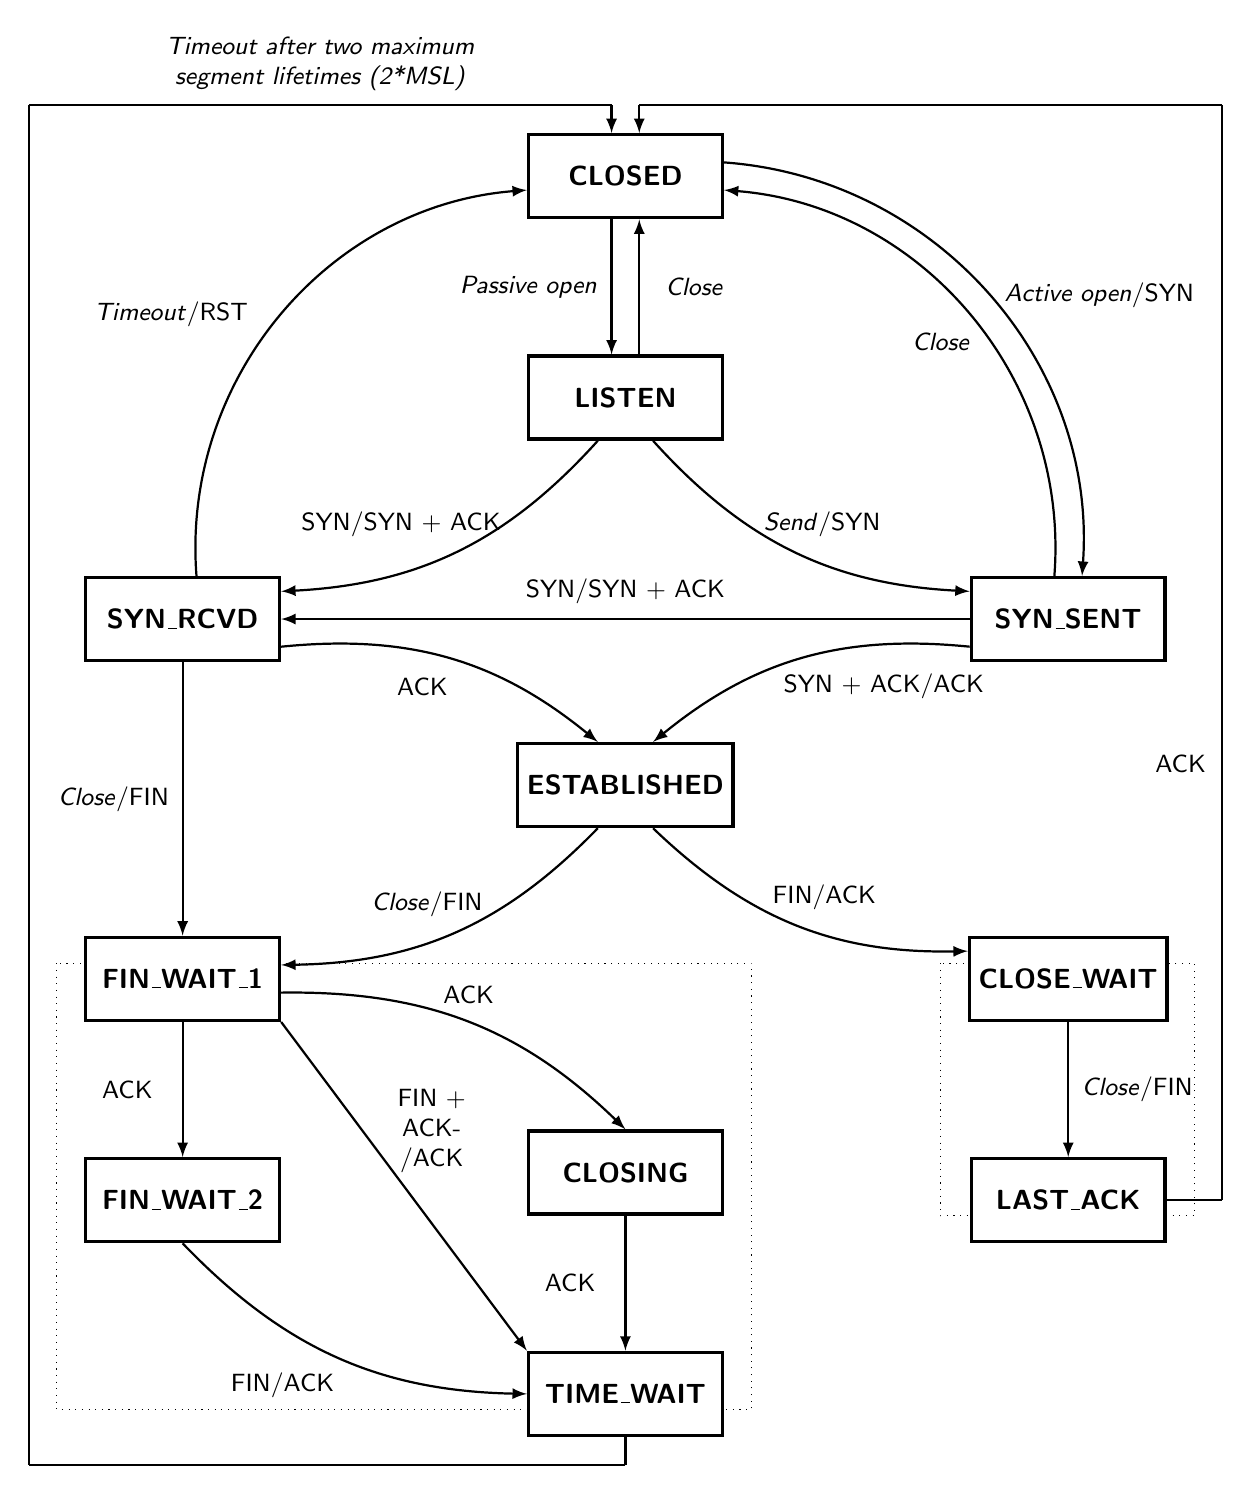
\begin{tikzpicture}[>=latex]

		%
		% Styles for states, and state edges
		%
		\tikzstyle{state} = [draw, very thick, fill=white, rectangle, minimum height=3em, minimum width=7em, node distance=8em, font={\sffamily\bfseries}]
		\tikzstyle{stateEdgePortion} = [black,thick];
		\tikzstyle{stateEdge} = [stateEdgePortion,->];
		\tikzstyle{edgeLabel} = [pos=0.5, text centered, font={\sffamily\small}];

		%
		% Position States
		%
		\node[state, name=closedStart] {CLOSED};
		\node[state, name=listen, below of=closedStart] {LISTEN};
		\node[state, name=synSent, below of=listen, right of=listen, xshift=8em] {SYN\_SENT};
		\node[state, name=synRcvd, below of=listen, left of=listen, xshift=-8em] {SYN\_RCVD};
		\node[state, name=established, below of=listen, node distance=14em] {ESTABLISHED};
		\node[state, name=finWait1, below of=established, left of=established, node distance=7em, xshift=-9em] {FIN\_WAIT\_1};
		\node[state, name=finWait2, below of=finWait1] {FIN\_WAIT\_2};
		\node[state, name=closeWait, below of=established, right of=established, node distance=7em, xshift=9em] {CLOSE\_WAIT};
		\node[state, name=closing, below of=established, node distance=14em] {CLOSING};
		\node[state, name=lastAck, below of=closeWait] {LAST\_ACK};
		\node[state, name=timeWait, below of=closing] {TIME\_WAIT};

		%
		% Connect States via edges
		%
		\draw ($(closedStart.south) + (-.5em,0)$)
		edge[stateEdge] node[edgeLabel, xshift=-3em]{\emph{Passive open}}
		($(listen.north) + (-.5em,0)$);
		\draw ($(listen.north) + (.5em,0)$)
		edge[stateEdge] node[edgeLabel, xshift=2em]{\emph{Close}}
		($(closedStart.south) + (.5em,0)$);

		\draw ($(listen.south) + (-1em,0)$)
		edge[stateEdge, bend left=22.5] node[edgeLabel, xshift=-2em, yshift=1em]{SYN/SYN + ACK}
		($(synRcvd.east) + (0,1em)$);
		\draw ($(listen.south) + (1em,0)$)
		edge[stateEdge, bend right=22.5] node[edgeLabel, xshift=1em, yshift=1em]{\emph{Send}/SYN}
		($(synSent.west) + (0,1em)$);

		\draw ($(synRcvd.north) + (.5em,0)$)
		edge[stateEdge, bend left=45] node[edgeLabel,xshift=-4em]{\emph{Timeout}/RST}
		($(closedStart.west) + (0,-.5em)$);

		\draw ($(synSent.north) + (-.5em,0)$)
		edge[stateEdge, bend right=45] node[edgeLabel,xshift=-1em, yshift=-1em]{\emph{Close}}
		($(closedStart.east) + (0,-.5em)$);
		\draw ($(closedStart.east) + (0,.5em)$)
		edge[stateEdge, bend left=45] node[edgeLabel,xshift=4em]{\emph{Active open}/SYN}
		($(synSent.north) + (.5em,0)$);

		\draw (synSent.west)
		edge[stateEdge] node[edgeLabel, yshift=1em]{SYN/SYN + ACK}
		(synRcvd.east);
		\draw (synRcvd)
		edge[stateEdge] node[edgeLabel, xshift=-2.5em]{\emph{Close}/FIN}
		(finWait1);

		\draw ($(synRcvd.east) + (0,-1em)$)
		edge[stateEdge, bend left=22.5] node[edgeLabel, xshift=-1em, yshift=-1em]{ACK}
		($(established.north) + (-1em,0)$);
		\draw ($(synSent.west) + (0,-1em)$)
		edge[stateEdge, bend right=22.5] node[edgeLabel, xshift=3em, yshift=-1em]{SYN + ACK/ACK}
		($(established.north) + (1em,0)$);

		\draw ($(established.south) + (-1em,0)$)
		edge[stateEdge, bend left=22.5] node[edgeLabel, xshift=-1em, yshift=1em]{\emph{Close}/FIN}
		($(finWait1.east) + (0,.5em)$);
		\draw ($(established.south) + (1em,0)$)
		edge[stateEdge, bend right=22.5] node[edgeLabel, xshift=1em, yshift=1em]{FIN/ACK}
		($(closeWait.west) + (0,1em)$);

		\draw (finWait1.south)
		edge[stateEdge] node[edgeLabel, xshift=-2em]{ACK}
		(finWait2.north);
		\draw ($(finWait1.east) + (0,-.5em)$)
		edge[stateEdge, bend left=22.5] node[edgeLabel, yshift=1em]{ACK}
		(closing.north);
		\draw (finWait1.south east)
		edge[stateEdge] node[edgeLabel, xshift=1em, yshift=2em, text width=3em]{FIN + ACK/ACK}
		(timeWait.north west);

		\draw (finWait2.south)
		edge[stateEdge, bend right=22.5] node[edgeLabel, xshift=-2em, yshift=-1em]{FIN/ACK}
		(timeWait.west);

		\draw (closing)
		edge[stateEdge] node[edgeLabel, xshift=-2em]{ACK}
		(timeWait);

		\draw (closeWait)
		edge[stateEdge] node[edgeLabel,xshift=2.5em]{\emph{Close}/FIN}
		(lastAck);

		%
		% Connect lastAck to closed is slightly more complicated
		% no direct line-of-sight, so we need to take the scenic route
		%
		\coordinate (lastAck2ClosedA) at ($(lastAck.east) + (2em,0)$);
		\coordinate (lastAck2ClosedB) at ($(closedStart.north -| lastAck.east) + (2em,1em)$);
		\coordinate (lastAck2ClosedC) at ($(closedStart.north) + (0.5em,1em)$);
		\draw (lastAck.east) edge[stateEdgePortion] (lastAck2ClosedA);
		\draw (lastAck2ClosedA) edge[stateEdgePortion] node[edgeLabel,xshift=-1.5em, yshift=-4em]{ACK} (lastAck2ClosedB);
		\draw (lastAck2ClosedB) edge[stateEdgePortion] (lastAck2ClosedC);
		\draw (lastAck2ClosedC) edge[stateEdge] ($(closedStart.north) + (0.5em,0)$);

		%
		% likewise for timeWait to closed
		%
		\coordinate (timeWait2ClosedA) at ($(timeWait.south) + (0,-1em)$);
		\coordinate (timeWait2ClosedB) at ($(timeWait.south -| finWait2.west) + (-2em,-1em)$);
		\coordinate (timeWait2ClosedC) at ($(closedStart.north -| finWait2.west) + (-2em,1em)$);
		\coordinate (timeWait2ClosedD) at ($(closedStart.north) + (-0.5em,1em)$);
		\draw (timeWait.south) edge[stateEdgePortion] (timeWait2ClosedA);
		\draw (timeWait2ClosedA) edge[stateEdgePortion] (timeWait2ClosedB);
		\draw (timeWait2ClosedB) edge[stateEdgePortion] (timeWait2ClosedC);
		\draw (timeWait2ClosedC) edge[stateEdgePortion]
		node[edgeLabel, text width=12.25em, yshift=1.5em]{\emph{Timeout after two maximum segment lifetimes (2*MSL)}}
		(timeWait2ClosedD);
		\draw (timeWait2ClosedD) edge[stateEdge] ($(closedStart.north) + (-0.5em,0)$);

		% draw dotted lines around passive and active closes
		\begin{pgfonlayer}{background}
			\draw [join=round,black,dotted] ($(closeWait.north west) + (-1em, -1em)$) rectangle ($(lastAck.south east) + (1em, 1em)$);
			\draw [join=round,black,dotted] ($(finWait1.north west) + (-1em, -1em)$) rectangle ($(timeWait.south east) + (1em, 1em)$);
		\end{pgfonlayer}

	\end{tikzpicture}
\end{center}

图 13-8将FIN\_WAIT\_I、FIN\_WAIT\_2 以及 \verb|TIME_WAIT| 状态用一个方框括起来(至少是部分被括起来),称作“主动关闭”。它们表示当本地应用程序发起一个关闭请求时会进入
的状态集合。另外两个状态(CLOSE\_WAIT 与LAST\_ACK)被一个虚线框括起来,并标记为“被动关闭”。这些状态与等待一个节点确认一个 FIN 报文段并进行关闭相关。同时关闭
可以视为一种包含两个主动关闭的形式。此外,还使用了CLOSING状态。

图13-8中的11种状态名称(CLOSED、LISTEN、SYN\_SENT等)都是基于 UNIX、Linux、Windows 系统中 netstat命令所输出的名称。而这些名称则是参考了\href{https://www.rfc-editor.org/rfc/rfc0793}{[RFC0793]}中的
名称。CLOSED 状态并不能算作一个“官方”的状态,但在图13-8 中却被作为一个开始状态点和一个终止状态点。

从LISTEN 到 SYN\_SENT 的状态转换在TCP 协议中是合法的,但却不被伯克利套接字所支持,因此比较少见。从SYN\_RCVD返回到 LISTEN 的状态转换只有在 SYN\_RCVD状
态是由LISTEN 状态(在正常的场景中)而非 SYN\_SENT 状态转换而来的情况下才是正确的。这意味着,如果我们执行一个被动打开操作(进入LISTEN 状态),接收一个SYN,发
送一个带有ACK 确认的SYN(进入SYN\_RCVD状态),然后收到一个重置消息而非ACK,端点就会返回到 LISTEN 状态,并且等待另一个连接请求的到来。

图13-9不仅显示了正常TCP连接的建立与终止过程,还详细介绍了客户端与服务器经历的各种状态。它是图13-1 的简略版本,在显示相关状态的同时省略了选项与初始序列号
等细节。假设在图 13-9中左侧的客户端执行一个主动打开操作,而右侧的服务器执行一个被动打开操作。虽然根据前文的介绍由客户端负责执行主动关闭操作,但是通信的任何一方
都能够进行这项工作。

\subsection{ TIME\_WAIT 状态 }
\verb|TIME_WAIT|状态也称为2MSL等待状态。在该状态中,TCP 将会等待两倍于最大段生存期(Maximum Segment Lifetime, MSL)的时间,有时也被称作加倍等待。每个实现
都必须为最大段生存期选择一个数值。它代表任何报文段在被丢弃前在网络中被允许存在的最长时间。我们知道这个时限是有限制的,因为TCP 报文段是以IP数据报的形式传输的,IP数
据报拥有 TTL 字段和跳数限制字段。这两个字段限制了 IP 数据报的有效生存时间(参见第5章)。\href{https://www.rfc-editor.org/rfc/rfc0793}{[RFC0793]} 将最大段生存期设为2分钟。然而在常见实现中,最大段生存期的数值可
以为30秒、1分钟或者2分钟。在绝大多数情况下,这一数值是可以修改的。在Linux 系统中,\verb|net.ipv4.tcp_fin_timeout| 的数值记录了 2MSL 状态需要等待的超时时间(以秒为单位)。
在 Windows 系统,下面的注册键值也保存了超时时间:
\begin{lstlisting}[language=bash]
HKLM\SYSTEM\CurrentControlSet\Services\Tcpip\Parameters\TcpTimedWaitDelay
\end{lstlisting}
该键值的取值范围是30~300秒。对于 IPv6 而言,只需要将键值中的Topip 替换为 Topip6即可。

假设已设定 MSL 的数值,按照规则:当TCP执行一个主动关闭并发送最终的ACK 时,连接必须处于 \verb|TIME_WAIT| 状态并持续两倍于最大生存期的时间。这样就能够让 TCP 重新
发送最终的ACK以避免出现丢失的情况。重新发送最终的ACK 并不是因为TCP 重传了ACK(它们并不消耗序列号,也不会被TCP重传),而是因为通信另一方重传了它的FIN(它
消耗一个序列号)。事实上,TCP 总是重传 FIN,直到它收到一个最终的ACK。

另一个影响2MSL 等待状态的因素是当TCP 处于等待状态时,通信双方将该连接(客户端卫地址、客户端端口号、服务器I地址、服务器端口号)定义为不可重新使用。只有
当2MSL 等待结束时,或一条新连接使用的初始序列号超过了连接之前的实例所使用的最高序列号时\href{https://www.rfc-editor.org/rfc/rfc1122}{[RFC1122]},或者允许使用时间戳选项来区分之前连接实例的报文段以避免混淆时
IRFC619]],这条连接才能被再次使用。不幸的是,一些实现施加了更加严格的约束。在这些系统中,如果一个端口号被处于 2MSL 等待状态的任何通信端所用,那么该端口号将不能
被再次使用。清单 13-3与清单13-4展示了这一约束的相关例子。

许多实现与API都提供了绕开这一约束的方法。在伯克利套接字API 中,SO\_RBUSEADDR 套接字选项就支持绕开操作。它允许调用者为自己分配本地端口号,即使这个
端口号是某个处于2MSL 等待状态连接的一部分。我们还会发现,即使套接字(地址、端口号对)具有绕开机制,TCP的规则仍会防止该端口号被处于 2MSL等待状态的同一连接的其
他实例重新使用。当一个连接处于 2MSL 等待状态时,任何延迟到达的报文段都将被丢弃。因为一条连接是通过地址和端口号的4元组定义的。如果该连接处于 2MSL 等待状态,那么
它在这段时间内将不能被重新使用。当这条正确的连接最终被建立起来后,这条连接之前的实例所传输的延迟报文段是不能被当作新连接的一部分来解读的。

对于交互式应用程序而言,客户端通常执行主动关闭操作并进入 \verb|TIME_WAIT| 状态,服务器通常执行被动关闭操作并且不会直接进入\verb|TIME_WAIT|状态。其中的含义是,如果我们
终止一个客户端后立刻重新启动同一客户端,那么新的客户端也不能重新使用相同的本地端口号。通常来说,这并不成问题。因为客户端通常使用的是由操作系统分配的临时端口号,
而且它们也并不关心被分配的端口号究竞是什么(回忆一下,实际上出于安全考虑有一种推荐的随机方法 TRFC6056]。值得注意的是,由于一个客户端能够快速产生大量的连接(尤其
是针对同一个服务器),因此它不得不在临时端口号供应紧张时延迟一会儿来等待其他连接的终止。

对于服务器而言,情况则大不相同。它们通常使用一些知名的端口。如果我们终止一个已经建立了一条连接的服务器进程,然后立即尝试重新启动它,服务器不能力该程序的通信
端分配对应的端口号(它将会收到一个“地址已占用”的绑定错误)。这是因为当连接进入2MSL 等待状态时,端口号仍然是连接的一部分。根据系统对 MSL 数值的不同设定,服务
器可能需要花费1~4分钟才能重新启动。我们可以利用sock程序观察这一场景。在清单13-3中,我们启动服务器,从客户端连接该服务器,然后终止服务器。

如果一个 TCP 连接要被其他进程重新使用,它必须在 \verb|TIME_WAIT| 状态下完成 2MSL的延迟

当重新启动服务器时,程序会输出一条错误信息,显示由于地址已经被占用而导致它的端口号不能被绑定。实际上这也意味着该地址与端口号的组合已经被使用。这是由于前一个
连接处于 2MSL 的等待状态而造成的。根据前文所述,这是对于端口号的重复使用最严历的限制。netstat 命令输出的结果显示连接处于 \verb|TIME_WAIT| 状态。虽然客户端不像服务器一样
会遇到如此多的关于2MSL 等待状态的问题,但是依然能够通过让客户端指定自己的端口号来证明相同的问题是存在的,如清单13-4所示。

当端口号被其他处于 2MSL 等待状态的连接使用时,它不能被客户端重复使用

在第一次执行客户端时,我们利用-v选项查出分配给客户端的(临时的)本地端口号为2091。在第二次执行客户端时,我们利用-b选项告诉客户端将 2091作为自己的本地端口号
来替代操作系统分配的临时端口号。正如我们所期望的,客户端不能完成上述操作。因为端口 2091 是一个处于 2MSL 等待状态的连接的不可分割部分。一旦等待结束(在Linux 机器
上为1分钟),客户端会尝试再次连接,但是服务器会在连接被首次中断后退出,所以该次尝试会被拒绝。本书将在13.6 节继续介绍如何利用 TCP的重置报文段表明连接被拒绝的条件。

前文曾经提到过,大多数系统会提供一种优先级高于默认行为的方式,这样即使某些端口是处于2MSL等待状态的连接的一部分,仍然允许进程对其进行绑定。现在我们在与之前
相同的场景下,利用sock 的-A选项来实现上述的绕开机制:

在此例中,我们在启动服务器时使用了-A选项,从而激活了之前提到过的SO\_RBUSEADDR套接字选项。通过这种方法,即使连接处于 2MSL 等待状态,它的端口仍然
能够被服务器绑定。如果我们马上使用具有相同端口号的客户端,将会发生下面的情况:

系统再一次提示了端点 127.0.0.1.32840正被使用,启动客户端失败。但是,如果我们也对客户端使用-A 选项,则能够强制该连接工作:

此处说明了即使重新使用处于 2MSL 等待状态的同一个连接(包括4元组),利用-A选项也能够强制该连接执行。当然,这些都发生在同一台计算机上,操作系统能够查明那些处
于2MSL 等待状态的(至少是潜在的)进程对应着连接的哪一端,并且使它们彼此间相互独立。如果在另一台主机上尝试相同的操作来建立一个连接会出现什么情况呢?下面将根据这
一想法进行测试:

除了客户端与服务器在不同的主机上之外,上述例子与之前的类似。如果不考虑客户端的-A选项,2MSL 等待时间是存在的。此处,2MSL 持续了30s的等待时间。此后,客户端
才会尝试联系服务器,然而此时服务器已经退出。

如果将客户端与服务器的计算机对换将会出现一些有趣的情况。现在,我们将 Windows
系统作为服务器而 Linux 系统作客户端,然后让它们重复上面的实验:

此时,我们希望本地端口32843是不可用的,但是由于在Linux 上运行了-A选项,所以可以使用这个端口。这一点违背了最初的TCP 规范,但如前文所述,它是被\href{https://www.rfc-editor.org/rfc/rfc1122}{[RFC1122]}
与\href{https://www.rfc-editor.org/rfc/rfc6191}{[RFC6191]}所允许的。如果有充足的理由相信新连接的报文段不会因为序列号、时间戳等问题与之前连接实例的报文段相混淆,那么在当前连接尚处在 \verb|TIME_WAIT| 状态时上述说明
会允许一条新连接的到达。\href{https://www.rfc-editor.org/rfc/rfc1337}{[RFC1337]}与\href{https://www.rfc-editor.org/rfc/rfc1323}{[RFC1323]} 的附录部分列出了与上述这条规则相关的常见错误。
\subsection{静默时间的概念}
在本地与外地的IP 地址、端口号都相同的情况下,2MSL 状态能够防止新的连接将前一个连接的延迟报文段解释成自身数据的状况。然而,上述方法只有在与处于 2MSL 等待状态
的连接相关的主机未关闭的条件下才具有意义。

如果一台与处于 \verb|TIME_WAIT| 状态下的连接相关联的主机崩溃,然后在 MSL 内重新启动,并且使用与主机崩溃之前处于 \verb|TIME_WAIT| 状态的连接相同的IP 地址与端口号,那么
将会怎样处理呢?在上述情况下,该连接在主机崩溃之前产生的延迟报文段会被认为属于主机重启后创建的新连接。这种处理方式将不会考虑在主机重启之后新连接是如何选择初始序
列号的。

为了防止上述情况的发生,\href{https://www.rfc-editor.org/rfc/rfc0793}{[RFC0793]}指出在崩溃或者重启后TCP 协议应当在创建新的连接之前等待相当于一个 MSL 的时间。该段时间被称作静默时间。然而只有极少数实现
遵循了这一点。因为绝大多数的主机在崩溃之后都需要超过一个 MSL 的时间才能重新启动。此外,如果上层应用程序自身已采用了校验和或者加密手段,那么此类错误会很容易检测
出来。
\subsection{ FIN\_WAIT\_2 状态}
在\verb|FIN_WAIT_2|状态,某TCP通信端已发送一个 FIN并已得到另一端的确认。除非出现半关闭的情况,否则该TCP端将会等待另一端的应用程序识别出自己已接收到一个文件
末尾的通知并关闭这一端引起发送 FIN的连接。只有当应用程序完成了这一关闭操作(它的FIN 已经被接收),正在关闭的TCP 连接才会从 \verb|FIN_WAIT_2|状态转移至 \verb|TIME_WAIT| 状态。
这意味着连接的一端能够依然永远保持这种状态。另一端也会依然处于 \verb|CLOSE_WAIT|状态,并且能永远维持这一状态直到应用程序决定宣布它的关闭。

目前有许多方法都能够防止连接进入 \verb|FIN_WAIT_2|这一无限等待状态:如果负责主动关闭的应用程序执行的是一个完全关闭操作,而不是用一个半关闭来指明它还期望接收数据,
那么就会设置一个计时器。如果当计时器超时时连接是空闲的,那么 TCP连接就会转移到CLOSED状态。在Linux 系统中,能够通过调整变量 \verb|net.ipv4.top_fin_timeout| 的数值来设置
计时器的秒数。它的默认值是 60s。
\subsection{同时打开与关闭的转换}
前文已经分别介绍了在发送与接收 SYN报文段时 \verb|SYN_SENT|状态与\verb|SYN_RCVD|状态的用途。如图13-3所示,TCP 协议经过专门的设计后能够处理同时打开的情况,并且只建
立一条连接。当同时打开的情况发生时,TCP 的状态迁移过程不同于图13-9的例子。通信的两端几乎在相同的时刻都会发送一个 SYN 报文段,然后它们进入 \verb|SYN_SENT|状态。当它
们接收到对方发来的SYN报文段时会将状态迁移至\verb|SYN_RCVD|,然后重新发送一个新的SYN 并确认之前接收到的SYN。当通信两端都接收到了 SYN与ACK,它们的状态将都会
迁移至 ESTABLISHED。

图13-4描述了TCP 同时关闭的情况。当应用程序发布关闭连接的消息后,通信两端的状态都会从 ESTABLISHBD 迁移至 \verb|FIN_WAIT_1|。与此同时,它们都会向对方发送一个
FIN。在接收到对方发来的FIN后,本地通信端的状态将从 \verb|FIN_WAIT_1|迁移至 CLOSING。然后,通信双方还会发送最终的ACK。当接收到最终的ACK 后,每个通信端会将状态更改
为\verb|TIME_WAIT|、从而初始化 2MSL等待过程。
\section{重置报文段}
第12章介绍了 TCP 头部的 RST 位字段。一个将该字段置位的报文段被称作“重置报文段”或简称为“重置”。一般来说,当发现一个到达的报文段对于相关连接而言是不正确的
时,TCP 就会发送一个重置报文段。(此处,相关達接是指由重置报文段的 TCP 与IP头部的4元组所指定的连接)。重置报文段通常会导致 TCP 连接的快速拆卸。本文将构建一些场景
来证明重置报文段的用途。
\subsection{针对不存在端口的连接请求}
通常情况下,当一个连接请求到达本地却没有相关进程在目的端口侦听时就会产生一个重置报文段。之前在“连接被拒绝”的错误消息中已经介绍过这种情况。这些均与TCP 协议
相关。根据第10章的内容,UDP 协议规定,当一个数据报到达一个不能使用的目的端口时就会生成一个ICMP 目的地不可达(端口不可达)的消息。TCP 协议则使用重置报文段来代
替完成相关工作。

这样的例子不胜枚举。例如,我们可以使用 \verb|telnet| 客户端并指定一个在目的主机上尚未使用的端口号。这台目的主机也可以是本地的计算机:

\verb|telnet| 客户端会快速地输出上述错误消息。清单 13-5显示了与此命令相关的数据包交换过程。

清单13-5中需要查看的数值包括重置(第2个)报文段中的序列号字段与ACK 号字段。由于到达的SYN 报文段未打开 ACK 位字段,重置报文段的序列号字段被设置为0,而ACK
号的大小则等于接收到的初始序列号加上该报文段中数据的字节数。虽然到达的报文段中并不含有任何数据,SYN 位在逻辑上仍会占用一个字节的序列号空间。因此,在这个例子中重
置报文段中的ACK 号等于初始序列号加上数据长度0,再加上SYN位的1字节。

对于一个被 TCP 端接收的重置报文段而言,它的ACK位字段必须被置位,并且 ACK号字段的数值必须在正确窗口的范围内(参见第12章)。这样有助于防止一种简单的攻击。
在这种攻击中任何人都能够生成一个与相应连接(4元组)匹配的重置报文段,从而扰乱这个连接 \href{https://www.rfc-editor.org/rfc/rfc5961}{[RFC5961]}。
\subsection{终止一条连接}
从图13-1可以看出终止一条连接的正常方法是由通信一方发送一个\verb|FIN|。这种方法有时也被称为\emph{\color{purple}有序释放}。因为FIN是在之前所有排队数据都已发送后才被发送出去,通常不会
出现丢失数据的情况。然而在任何时刻,我们都可以通过发送一个重置报文段替代\verb|FIN|来终止一条连接。这种方式有时被称作\emph{\color{purple}终止释放}。

终止一条连接可以为应用程序提供两大将性:(1)\emph{任何排队的数据都将被抛弃,一个重置报文段会被立即发送出去};(2)\emph{重置报文段的接收方会说明通信另一端采用了终止的方式
而不是一次正常关闭}。API必须提供一种实现上述终止行为的力式来取代正常的关闭操作。

套接字API通过将“逗留于关闭”套接字逃项(\verb|SO_LINGER|)的数位设置为0来实现上述功能。从本质上说,这意味着“不会在终止之前为了确定数据是否到达另一端而逗留任
何时间”。下面的例子尽示了当一个产生大量输出的远程命令被用户取消时所发生的状况:
\begin{lstlisting}[language=bash, caption=Hello world program., label=listing:hello_world]
	Linux%: ssh linux cat /usr/share/dict/words
	Aarhus
	Aaron
	Ababa
	aback
	abaft
	aband゜n
	abandoned
	aband゜nin9
	abandorment
	abandons
	... continues ...
	^C
	Killed by signa1 2.
\end{lstlisting}

此处,用户决定终止这条命令的输出行为。由于单词文件中包含了 45427 个字,这个命令很可能是某种错误。当用户键入中断字符时,系统显示对应进程(此处为 ssh 程序)已经被
2号信号终止。该信号被称作SIGINT,常用于终止一些交付的程序。清单13-6显示了上述例子中 tcpdump 的相应输出结果(由于与本文的讨论无关,大量的中间数据包已被删除)。

报文段1~3显示了正常连接的建立过程。当中断字符被键入之后,连接被终止。重置报文段中包含了一个序列号写一个确认号。还需要注意的是重置报文段不会令通信另一端做
出任何响应——它不会被确认。接收重置报文段的一端会终止连接并通知应用穆序当前连接已被重置。这样通常会造成“连接被另一端重置”的错误提示或类似的消息。
\subsection{半开连接}
如果在未告知另一端的情况下通信的一端关闭或终止连接,那么就认为该条 TCP 连接处于半开状态。这种情况发生在通信一方的主机崩溃的情况下。只要不尝试通过半开连接传
输数据,正常工作的一端将不会检测出另一端已经崩溃。

产生半开连接的另一个共同原因是某一台主机的电源被切断而不是被正常关机。这种情况可能发生于下面的例子中:某些个人电脑运行了远程登录客户端,并且在一天结束时关闭。
如果在电源被切断时没有数据在传输,那么服务器永远也不会知道该客户端已经消失(它可能还一直会认为该连接处于 ESTABLISHED 状态)。当第二天早晨用户回来,启动电脑并开
始一个新的会话时,服务器会启动一个新的服务进程。这样会导致服务器上有很多半开的TCP连接(第17章将会介绍一种方法,使TCP连接的一端能够利用 TCP 的keepalive 选项
发现另一端已经消失)。

我们能够很容易地创建一个半开连接。在这种情况下,将在客户端而不是服务器做一些尝试。我们在主机 \verb|10.0.0.1| 上执行 \verb|telnet| 客户端程序,连接 Sun 公司提供远程过程调用服务
(sunrpc,端口号 111)的服务器。如清单13-7所示,该服务器的IP 为10.0.0.7。我们键人一行输人,并利用 tcpdump 观察它们的交互过程,然后断开服务器主机的以太网连接并重新启
动这台主机。这样就能模拟服务器崩溃的情况。(我们在重启服务器之前断开以太网连接是为了防止其通过已开启的连接发送一个 FIN。一些TCP 会在其关闭时完成上述操作。)在服
务器重启之后,我们重新连接以太网并且尝试从客户端向服务器发送另一行命令。在重启之后,服务器的TCP会丢失之前所有连接的记忆,因此它对数据段中指出的这条连接一无所
知。此时,TCP规定接收者将回复一个重置报文段作为响应。

服务器主机被切断连接后重启,留给客户端一个半开的连接。当再次从这条连接上接收到其他数据时,服务器对其一无所知。在服务器回复一个重置报文段作为响应之后,两端之间的连接会被关闭

清单 13-8显示了该例的 tcpdump 输出。

报文段1~3描述了正常的连接建立过程。报文段4将“foo”行发送至 sunrpe服务器(包括回车符与换行符共需要5个字节)。报文段5则完成确认工作。

此时,我们断开服务器端(地址 10.0.0.7)的以太网连接,然后重启服务器并重新接人以太网。上述操作大约花费90秒的时间。然后,我们在客户端键入一行新的输人(“bar”)。
当我们按下回车键后,这一行输入将会发送至服务器(如清单13-9所示,在ARP 流量之后的第一个 TCP报文段中)。由于该服务器不再记得之前的这条连接,所以上述操作将引起服
务器端的重置响应。

需要注意的是当主机重新启动时,它将使用免费的ARP 协议(参见第4章)来确定自己的IPv4地址是否已经被其他报文段使用,而这些报文段是属于其他主机的。它还会请求与
I地址\verb|10.0.0.1| 对应的MAC地址,因为这是它对于 Internet 的默认路由。

\subsection{时间等待错误}
如前文所述,设计 \verb|TIME_WAIT| 状态的目的是允许任何受制于一条关闭连接的数据报被丢弃。在这段时期,等待的 TCP通常不需要做任何操作,它只需要维持当前状态直到2MSL
的计时结束。然而,如果它在这段时期内接收到来自于这条连接的一些报文段,或是更加特殊的重置报文段,它将会被破坏。这种情况被称作时间等待错误(TIME-WAIT AsSassination
TWA,参见\href{https://www.rfc-editor.org/rfc/rfc1337}{[RFC1337]})。图13-10展示了数据包的交换过程。

一个重置报文段能“破坏”\verb|TIME_WAIT|状态并强制连接提前关闭。目前有很多方法来阻止这一问题,其中包括在处于 \verb|TIME_WAIT| 状态时忽略重置报文段

在图13-10的例子中,服务器完成了其在连接中的角色所承担的工作并清除了所有状态。客户端依然保持 \verb|TIME_WAIT|状态。当完成FIN 交换,客户端的下一个序列号为K,而
服务器的下一个序列号为L。最近到达的报文段是由服务器发送至客户端,它使用的序列号为L-100,包含的ACK号为K-200。当客户端接收到这个报文段时,它认为序列号与
ACK 号的数值都是“旧”的。当接收到旧报文段时,TCP 会发送一个 ACK 作为响应,其中包含了最新的序列号与ACK 号(分别是K与L)。然而,当服务器接收到这个报文段以后,
它没有关于这条连接的任何信息,因此发送一个重置报文段作为响应。这并不是服务器的问题,但它却会使客户端过早地从 \verb|TIME_WAIT|状态转移至 CLOSED状态。许多系统规定当
处于 \verb|TIME_WAIT| 状态时不对重置报文段做出反应,从而避免了上述问题。
\section{TCP 服务器选项}
第1章曾介绍过,大多数TCP服务器是并发的。当一个新的连接请求到达服务器时,服务器接受该连接,并调用一个新的进程或线程来处理新的客户端。根据不同的操作系统,各
种其他的资源也可以被分配来调用新的服务器。我们对多个并发服务器间的 TCP 交互非常感兴趣,尤其希望了解 TCP服务器是如何使用端口号的,以及如何处理多个并发客户端的。
\subsection{TCP端口号}
可通过观察任何一台 TCP服务器来了解 TCP 是如何处理端口号的。在一台拥有 IPv4与IPv6 双协议栈的主机上利用 netstat 命令观察安全外壳服务器(也称作 sshd)。sshd 应用程序
执行的是安全外壳协议\href{https://www.rfc-editor.org/rfc/rfc4254}{[RFC4254]}。该协议能够提供可加密认证的远程终端功能。下面的输出结果来自于没有主动安全外壳连接的系统(除了与服务器相关的输出外,其他所有的输出
行都已被删除):
-a选项能够报告所有的网络节点,包括那些处于侦听状态和未处于侦听状态的节点。-n选项以点分十进制(或十六进制)数的形式打印 IP地址,而不会试图利用 DNS 将地址转换
为一个域名。此外,该选项还会打印数值端口号(例如22),而不是服务名(例如ssh)。-t选项用于只选择 TCP节点。

本地地址(这实际意味着本地节点)的输出结果为::22。这种面向 IPv6的方式表示的是全0地址,也被称作通配符地址,并使用端口号22。这意味着一个针对22号端口的连接进
入请求(即一个SYN)会被任何本地接口接受。如果主机是多宿主的(此例即是),我们可以为本地 IP 地址指定一个单一的地址(主机IP 地址中的一个地址),并且只有被该接口接收到
的连接才能够被接受(参见本节后面的例子)。端口号22是为安全外壳协议预留的知名端口号。其他端口号是由网络编号分配机构(ITNA)来维护的。

外部地址的输出结果为:*,这表示一个通配符地址与端口号(即,一个通配符节点)。此处由于本地节点处于 LISTEN状态,正等待一个连接的到来,因此外部地址与外部端口号
尚不知晓。现在我们在主机10.0.0.3上启动一个安全外壳客户端来连接该服务器。下面是从netstat 输出的相关行(RECV-Q 与Send-Q列只包含零值,为清楚起见,将其删除):

标有端口号 “22”的第2行是一个 ESTABLISHED 连接。本地与外地节点相关的4元组都会填写在这个连接中,其中包括:本地 IP地址与端口号,外地IP地址与端口号。本地IP
地址与连接请求到达的接口相关(以太网接口通过与IPv4地址映射的IPv6地址:fft:\verb|10.0.0.1|进行标识)。

处于 LISTEN 状态的本地节点会独自地运行。它用于为并发服务器接收未来可能出现的请求。当有新的连接请求到达并被接收时,操作系统中的 TCP 模块创建处于 ESTABLISHBD
状态的新节点。同样需要注意的是,当连接处于 ESTABLISHBD 状态时,它的端口号仍为22,与LISTEN 状态时相同。

现在我们从同一个系统(10.0.0.3)向服务器发送另一个客户端请求。相关的 netstat 输出如下:

现在我们有两个处于ESTABLISHED状态的连接。它们以同一个客户端到相同的服务器端。两条连接的服务器端口号均为22。由于外地端口号不同,因此这并不算是一个TCP错
误。这两个外地端口必须是不同的。因为每个安全外壳程序使用的是一个临时端口,而每一个临时端口在定义时都是主机(10.0.0.3)尚未使用的端口。

这个例子再次说明TCP依靠4元组多路分解(demultiplex)了获得的报文段。目的IF地址与目的端口号、源1地址与源端口号,这4元组共同构成了本地与外地节点。TCP协
议不能仅仅根据目的端口号来决定哪一个进程该得到接收的报文段。在所有三个节点中只有位于端口22 的节点会处于 \verb|LISTEN| 状态并接收进入的连接请求。处于 ESTABLISHED 状态
的节点不能接收 SYN 报文段,而处于 LISTEN 状态的节点则不能接收数据段。例子中主机的操作系统已经证实了这一点。(如果不能如此,TCP 就会变得非常混乱,从而不能正常地
工作)。

下面我们发起第三个客户端连接。这条连接来自 IP 地址 169.229.62.97,通过DSLPPPoE 链路与服务器\verb|10.0.0.1| 相连。因此这个客户端与服务器不处于同一个以太网。(为了清
楚起见,下面的输出结果移除了 Proto 列,只留下了 tcp部分。)

在这台多宿主的主机上,第三条 ESTABLISHED 连接的IP地址与 PPPoE链路的接口地址(67.125.227.195)相关联。值得注意的是 Send-Q状态的数值并不是0,而是被928字节
所代替。这意味着服务器已经在这条连接上发送了928字节的数据但仍然未收到任何确认。
\subsection{限制本地 IP地址}
本节将介绍当服务器不能借助通配符处理某个本地IP地址而将其设置为一个特殊的本地地址时发生的情况。如果我们将 sock 程序当作服务器运行并为其提供一个特殊的IP地址,
那么该地址将成为监听端的本地 IP 地址。例如:

这样就限制了服务器只能使用到达本地IPv4 地址 \verb|10.0.0.1| 的连接。下面 netstat 的输出结果反映了这一点:

在上述例子中特别有趣的是我们的sock 程序只与本地IPv4.地址\verb|10.0.0.1|绑定,所以netstat 的输出结果与之前不同。在之前的例子中,通配符地址与端口号标识了两种版本的IP
地址。在这种情况下,我们绑定了一个特殊的地址、端口或地扯族(只适用IPv4)。如果我们从本地网络连接这台服务器,比如从主机10.0.0.3,那么正常工作的记录情况如下:

如果我们从一台目的地址不是\verb|10.0.0.1|(甚至包括本地地址127.0.0.1)的主机连接服务器,连接请求将不会被 TCP模块接收。如果我们查看 \verb|tcpdump|,SYN 会引发一个 RST报文
段,如清单 13-9所示。

服务器的应用程序将不会察觉到连接请求\textemdash 因为拒绝接收的操作是由操作系统的TCP模块根据该应用程序指定的本地IP地址与SYN报文段中包含的目的地址做出的。我们发现
限制本地IP 地址的能力是相当严格的。
\subsection{限制外部节点}
根据第10章的介绍,一台UDP服务器不仅能够指定本地IP地址与本地端口号,还能够指定外部 IP 地址与外部端口号。\href{https://www.rfc-editor.org/rfc/rfc0793}{[RFC0793]}所介绍的 TCP 的抽象接口函数允许一台服务
器为一个完全指定的外部节点(等待一个特定的客户端以发起一个主动打开)或者一个未被指定的外部节点(等待任何客户端)执行被动打开。

不幸的是,普通的伯克利套接字 API 没有提供实现这一点的方法。服务器不必指定客户端的节点,而是等待连接的到来,然后检查客户端的IP地址与端口号。表13-3概括了TCP
服务器能够建立的三种类型的地址绑定。

在上述例子中,\verb|local_port|是服务器被分配的端口号,而\verb|local_IP|必须是一个应用于本地系统的单播 IP地址。表13-3中三行的排列顺序显示了当收到一个连接请求时 TCP 模块
决定选择哪一个节点的次序。最明确的绑定(第1行,如果支持的话)将会被首先尝试,而最不明确的绑定(最后一行,所有的IP地址都用通配符表示)将会被最后尝试。对于同时
支持IPv4 与IPv6 双协议栈的系统,它的端口号空间可能会出现混合的情况。从本质上说,这意味着如果服务器使用IPv6地址绑定了一个端口号,那么也就将该端口号应用于了IPv4
地址。
\subsection{进入连接队列}
一个并发的服务器会为每一个客户端分配一个新的进程或线程,这样负责侦听的服务器能够始终准备着处理下一个到来的连接请水。这是使用并发服务器的根本原因。然而,在侦
听服务器正创建一个新进程时,或者在操作系统忙于运行其他高优先级的进程时,甚至更糟的是在服务器正在被伪造的逐接请求(这些伪造的建立连接请求是不被允许的)攻击时,多
个连接请求可能会到达。在这些情况下,TCP成当如何处理呢?

为了充分探讨这个问题,我们首先必须认识到,在被用于应用程序之前新的连接可能会处于下述两个状态。一种是连接尚未完成但是已经接收到 SYN(也就是处于 \verb|SYN_RCVD|状
态)。另一种是连接已经完成了三次据手并且处于 ESTABLISHED状态,但还未被应用程序接受。因此在内部操作系统通常会使用两个不同的连接队列分别对应上述两种不同的情况。

应用程序通过限制这些队列的大小来进行控制。传统上,使用伯克利套接字 API 应用程序只能间接地控制这两个队列的大小总和。在现代的Linux内核中,这种行为已更改为第二
种状况下的连接数目(ESTABLISHED 状态的连接)。因此,应用程序能够限制完全形成的等待处理的连接数目。在Linux 中,将会适用以下规则:
\begin{enumerate}
	\item 当一个连接请求到达(即,SYN报文段),将会检查系统范围的参数 \verb|net.ipv4.tcp_max_syn_| \verb|backlog|(默认为1000)。如果处于\verb|SYN_RCVD|状态的连接数目超过了这一阙值,进入的连接将会被拒绝。
	\item 每一个处于侦听状态下的节点都拥有一个固定长度的连接队列。其中的连接已经被 TCP 完全接受(即三次握手已经完成),但未被应用程序接受。应用程序会对这一队列做出限制,通常称为未完成连接(backlog)。backlog 的数目必须在0与一个系统指定的最大值之间。
	      该最大值称为 \verb|net.core.somaxconn|,默认值128(包含)。
	      需要记住的是backlog的数值指出了一个侦听节点中排队连接的最大数目,所有这些连接已经被TCP接受并等待应用程序接受。无论对系统所允许的已经建立连接的最大数目,还是对一个并行服务器所能同时处理的客户端数目,backlog 都不会造成影响。
	\item 如果侦听节点的队列中仍然有空间分配给新的连接,TCP 模块会应答 SYN并完成连接。直到接收到三次握手中的第3个报文段之后,与侦听节点相关的应用程序才会知道新的连接。当客户端的主动打开操作顺利完成之后,客户端可能会认为服务器已经准备好接收数据,然而服务器上的应用程序此时可能还未收到关于新连接的通知。如果这种情况发生,服务器的TCP模块将会把到来的数据存人队列中。
	\item 如果队列中已没有足够的空间分配给新的连接,TCP 将会延迟对SYN 做出响应,从而给应用程序一个跟上节奏的机会。Linux 在这一方面有着独特的行为——它坚持在能力允许的范围内不忽略进入的连接。如果系统控制变量 \verb|net.ipv4.tcp_abort_on_overflow| 已被设定,新进入的连接会被重置报文段重新置位。
\end{enumerate}

在队列溢出的情况下,发送重置报文段通常是不可取的,而且默认情况下这项功能也不会打开。客户端会尝试与服务器联系,如果它在交换 SYN 期间接收到一个重置报文段,那
么它可能会错误地认为没有服务器存在(而不是认为有一台服务器存在并且十分繁忙)。太忙实际上是一种“软”的或者暂时的错误,而不是一种硬性的错误。正常情况下,当队列已
满,应用程序或操作系统会十分繁忙,此时应当阻止应用程序再去服务那些进入的连接。上述状况可能会在短时间内得到改善。然而,如果一台服务器的 TCP使用重登报文段进行回
复,那么客户端将会放弃主动打开的操作(这与服务器没有启动时所看到的情况是类似的)。在不发送重置报文段的情况下,如果一台侦听的服务器始终无法抽出时间来接受那些已经被
TCP接受却超出队列保存上限的连接,那么根据正常的TCP 机制,寄户端的主动打开操作将会最终超时。在Linux 中,连接的客户端将会明显地放缓一段时间,它们既不会超时也
不会重置。

借助我们的sock程序,大家会看到当进入连接队列溢出后会发生的情况。我们利用一个新的选项(-O)来调用程序,并且告诉它在创建完侦听节点后暂停,直到接收到任何连接
请求。如果之后我们在暂停期间再调用多个客户端,服务器的接收连接队列将会被填满,因此可以借助 tcpdump 检查所发生的一切。

-q1选项将侦听节点的 \verb|backlog| 数值设置 1。-030000选项使程序在接收任何客户端连接之前先休眠30000秒(基本上是一个很长的时间,大约8小时)。如果我们现在不断地尝
试连接这台服务器,最早的4个连接将会被立即完成。此后两个连接需要9秒才能完成。其他操作系统在处理这种情况时会有明显的不同。例如在 Solaris8和 \verb|FreeBSD 4.7|中,两个连
接会被立即处理而第3个连接将会超时,而随后的连接也将超时。

清单13-10显示了用一台Linux 客户端连接一台 \verb|FreeBSD| 服务器的 \verb|tcpdump| 输出结果。\verb|FreeBSD| 服务器上运行着符合上文参数设定的 sock 程序(在TCP 连接建立时,即三次握手
完成时,已经用黑体标记了客户端的端口号)。

TCP 接受的第1个客户端连接请求来自端口2461(报文段1~3)。第2个客户端的连接请求来自端口 2462,也被TCP接受(报文段4~6)。服务器的应用程序仍处于睡眠状态,
不能够接受任何连接。所有的工作都是由操作系统的TCP模块来完成的。由于三次握手过程均已完成,这两个客户端都从主动打开成功地返回。

我们尝试开启第3个客户端,它的SYN报文段如清单13-10 中的第7个报文段所示(端口号2463),但由于侦听节点的队列已满,服务器端的 TCP 忽略了该SYN 报文段。客户端
根据二进制指数退避机制重新传输了它的SYN报文段,如清单13-10中的第8~12个报文段所示。在 FreeBSD 与 Solaris 系统中,TCP会在队列满后忽略进入的SYN 报文段。

据前文所述,如果侦听者的队列有足够的空间,TCP 将会接受一个进入的连接请求(即一个SYN报文段),而不会让应用程序去识别这条连接来自何方(源I地址与源端口号)。
这一点并不是TOP协议所要求的,而是通用的实现技术(即伯克利套接字的工作方式)。如果采用替代伯克利套接字 API 的方法(例如 TLi/XTI),能够为应用程序提供一种了解何时有
连接到达的方法,并允许它们选择是否接受到达的连接请求。TUI 只是在理论上提供这种能力,但未能完全付诸实践,因此伯克利套接字能够更有效地为TCP 接口提供文持。

在借助伯克利套接字实现的 TCP 中,当应用程序被告知一条连接已经到达时,TCP 的三次握手过程已经完成。上述行为也意味着一个 TCP 服务器无法让一个客户端的主动打开
操作失败。当一个新的客户端连接传达至服务器应用程序时,TCP的三次握手过程已经结束,而且客户端的主动打开操作已经成功完成。如果此后服务器查看了客户端的 IP地址与端口
号,并且决定不向该客户端提供服务,那它只能关闭(发送一个FIN)或者重置这系连接(发送一个RST)。无论处于上述哪一种情况,客户端在完成主动打开操作后都会认为一切正常,
甚至已经向服务器发出了请求。因此,需要其他传输层协议来为应用程序提供区分连接到达与接受的功能(即 OSI模型的传输层),但不是TCP。
\section{与 TCP 连接管理相关的攻击}
SYN 泛洪是一种TCP拒绝服务攻击,在这种攻击中一个或多个恶意的客户端产生一系列 TCP连接尝试(SYN报文段),并将它们发送给一台服务器,它们通常采用“伪造”的
(例如,随机选择)源IP地址。服务器会为每一条连接分配一定数量的连接资源。由于连接尚未完全建立,服务器为了维护大量的半打开连接会在耗尽自身内存后拒绝力后续的合法连
接请求服务。

\subsection{syncookie}
因为区分合法的连接尝试与SYN泛洪并不是一件容易的事情,所以抵御上述攻击存在一定的难度。一种针对此问题的机制被称作SYN cookies\href{https://www.rfc-editor.org/rfc/rfc4987}{[RFC4987]}。SYN cookies 的主要
思想是,当一个 SYN到达时,这条连接存储的大部分信息都会被编码并保存在SYN +ACK报文段的序列号字段。采用SYN cookies 的目标主机不需要进入的连接请求分配任何存储
资源—只有当SYN +ACK 报文段本身被确认后(并且已返回初始序列号)才会分配真正的内存。在这种情况下,所有重要的连接参数都能够重新获得,同时连接也能够被设置为
ESTABLISHED 状态。

在执行 SYN cookies 过程中需要服务器仔细地选择 TCP 初始序列号。本质上,服务器必须将任何必要的状态编码并存于 SYN+ACK 报文段的序列号字段。这样一个合法的客户端
会将其值作为报文段的ACK 号字段返回给服务器。很多方法都能够完成这项工作,下面将具体介绍 Linux 系统所采用的技术。

服务器在接收到一个 SYN 后会采用下面的方法设置初始序列号(保存于SYN +ACK 报文段,供于客户端)的数值:首5位是t模32的结果,其中t是一个32位的计数器,每隔
64秒增1;接着3位是对服务器最大段大小(8种可能之一)的编码值;剩余的24位保存了4元组与t值的散列值。该数值是根据服务器选定的散列加密算法计算得到的。

\begin{tcolorbox}[title = {Note}]
	linux 4.4 syncookie \href{https://elixir.bootlin.com/linux/v4.4.302/source/net/ipv4/syncookies.c#L108}{syncookie} 使用散列函数 sha1
\end{tcolorbox}

在采用SYN cookies 方法时,服务器总是以一个 SYN +ACK 报文段作为响应(符合任何典型的TCP 连接建立过程)。在接收到 ACK后,如果根据其中的:值可以计算出与加密
的散列值相同的结果,那么服务器才会为该SYN 重新构建队列。这种方法至少有两个缺陷。首先,由于需要对最大段大小进行编码,这种方法禁止使用任意大小的报文段。其次,由于
计数器会回绕,连接建立过程会因周期非常长(长于64秒)而无法正常工作。基于上述原因,这一功能并未作为默认设置。

\subsection{路径最大传输单元}
另一种攻击方法与路径最大传输单元发现过程相关。在这种攻击中,攻击者伪造一个ICMP PTB 消息。该消息包含了一个非常小的MTU 值(例如,68字节)。这样就迫使受害的
TCP 尝试采用非常小的数据包来填充数据,从而大大降低了它的性能。最粗暴的解决方法是简单地禁用主机的路径最大传输单元发现功能。当接收到的 ICMP PTB 消息的下一跳最大
传输单元小于576字节时,其他选项会禁用路径最大传输单元发现功能。还有一种Linux实现的方法,前文曾介绍过,是使最小的数据包大小(对 TCP 使用的大數据包)固定为某一数
据,并使较大的数据包不将 IPv4的DF 位置位。这种方法虽然比完全禁用路径最大传输单元发现功能更具吸引力,但也与其十分类似。

\subsection{hijiacking tcp}
另一种类型的攻击涉及破坏现有的 TCP 连接,甚至可能将其劫持(hijiacking)。这一类攻击通常包含的第一步是使两个之前正在通信的 TCP节点“失去同步”。这样它们将使用
不正确的序列号。它们是序列号攻击的典型例子\href{https://www.rfc-editor.org/rfc/rfc1948}{[RFC1948]}。至少有两种方法能实现上述攻击:在连接建立过程中引发不正确的状态传输(类似于13.6.4小节介绍的时间等待错误),在
ESTABLISHED 状态下产生额外的数据。一旦两端不能再进行通信(但却认为它们间拥有一个打开的连接),攻击者就能够在连接中注入新的流量,而且这些注人的流量会被TCP认为
是正确的。

\subsection{欺骗攻击}
有一类攻击被称作欺骗攻击。这类攻击所涉及的 TCP报文段是由攻击者精心定制的,目的在于破坏或改变现有 TCP连接的行为。在\href{https://www.rfc-editor.org/rfc/rfc4953}{[RFC4953]}中大量讨论了此类攻击及它们的
防治技术。攻击者可以生成一个伪造的重置报文段并将其发送给一个TCP通信节点。假定与连接相关的4元组以及校验和都是正确的,序列号也处在正确的范围。这样就会造成连接
的任意一端失败。随着互联网变得更快,为了维持性能被认为“处于窗口”的序列号范围也在不断地扩大(参见第15章),上述攻击也受到越来越多的关注。欺骗攻击还存在于其他类
型的报文段(SYAN,甚至 ACK)中(有时会与泛洪攻击结合使用),引发大量的问题。相关的防御技术包括:认证每一个报文段(例如,使用TCP-AO 选项);要求重置报文段拥有一个
特殊的序列号以代替处于某一范围的序列号;要求时间戳选项具有特定的数值;使用其他形式的 cookie 文件,让非关键的数据依赖于更加准确的连接信息或一个秘密数值。

欺骗攻击虽然不是 TCP 协议的一部分,但是能够影响 TCP 的运行。例如,ICMP 协议能够被用于修改路径最大传输单元的发现行为。它也能够被用于指出一个端口号或一台主机
已失效,从而终止一个 TCP 连接。\href{https://www.rfc-editor.org/rfc/rfc5927}{[RFC5927]}介绍了大量的此类攻击,并且还提出了一些防御ICMP 欺骗消息、提高鲁棒性的方法。这些建议不仅局限于验证ICMP 消息,而且还涉及
其可能包含的 TCP报文段。例如,包含的报文段应该拥有正确的4元组与序列号。
\section{总结}
在两个进程使用TCP 协议交换数据之前,它们必须要在彼此间建立一条连接。当数据传输完毕,它们将终止这条连接。本章详细介绍了连接是如何借助三次握手过程建立的,而
且又是如何利用4个报文段终止的。本章还介绍了TCP 是如何处理同时打开与关闭操作的,以及如何管理各个选项,其中包括选择性确认、时间戳、最大段大小、TCP认证以及用户超
时选项。

本章使用tcpdump 与 Wireshark 来显示TCP 协议的行为以及 TCP 头部字段的使用情况。还展示了连接的建立过程是如何超时的,重置报文段是如何发送与解析的,以及 TCP是如
何提供半打开与半关闭连接的。TCP既约束了在一个主动打开操作中尝试连接的改数,又约束了在一次被动打开操作后能服务的尝试连接次数。

TCP状态转换图对理解其运行非常重要。本章依次介绍了连接的建立、终止以及状态迁移的各个步骤。本章还介绍了并发 TCP服务器设计中 TCP 连接建立的相关工作。

一条TCP连接是由一个4元组唯一定义的,包括:本地IP地址,本地端口号,外部IP地址,外部端口号。每次连接终止时,通信一端必须维护这些相关信息。根据本章的介绍,
TCP 的\verb|TIME_WAIT|状态负责完成这些工作。规则是执行主动关闭操作的一端进入 \verb|TIME_WAIT|状态并维持两倍的最大段生存时间。这样有助于防止 TCP处理同一条连接中旧实例的
报文段。当新的连接尝试使用相同的4元组时,使用时间戳选项能够减少等待时间,另外它还有助于探测回绕的序列号以及更好地测量往返时间。

TCP 在资源耗尽与欺骗等攻击面前是十分脆弱的,但已研究出一些方法来抵御上述问题。此外,TCP还会受到其他协议的影响,比如ICMIP。通过仔细地分析ICMP 消息所返回
的原始数据报可以加强对ICMIP 的防御。最后,TCP 可以与其他协议结合使用,为协议栈的其他层提供安全支持(例如,IPsec 与 TLS/SSL,参见第18章),这已成为标准的做法。
\section{参考文献}

\chapter{TCP超时与重传}

\section{引言}
到目前为止,我们并没有过多地涉及效率与性能,而主要关注操作的正确性。在本章及接下来的两章中,我们不仅讨论 TCP执行的基本任务,还关心其执行效率。由于下层网络
层(IP)可能出现丢失、重复或失序包的情况,TCP 协议提供可靠数据传输服务。为保证数据传输的正确性,TCP重传其认为已丢失的包。TCP根据按收端返回至发送端的一系列确认
信息来判断是否出现丢包。当数据段或确认信息丢失,TCP启动重传操作,重传尚未确认的数据。TCP拥有两套独立机制来完成重传,一是\textbf{基于时间},二是\textbf{基于确认信息的构成}。第二
种方法通常比第一种更高效。

TCP 在发送数据时会设置一个计时器,若至计时器超时仍未收到数据确认信息,则会引发相应的超时或基于计时器的重传操作,计时器超时称为重传超时(RTO)。另一种方式的重
传称为快速重传,通常发生在没有延时的情况下。若 TCP 累积确认无法返回新的ACK,或者当ACK 包含的选择确认信息(SACK)表明出现失序报文段时,快速重传会推断出现丢
包。通常来说,当发送端认为接收端可能出现数据丢失时,需要决定发送新(未发送过的)数据还是重传。本章内容将详细讨论 TCP怎样判断出现报文段丢失及其响应操作。发送数
据量问题,即由丢包而引发的拥塞控制机制,将会在第16章具体介绍。这里,我们探讨如何根据某个连接的 RTT来设置 RTO,基于计时器的重传机制,以及TCP快速重传操作。另
外我们也会看到SACK 怎样帮助确定丢失数据、失序和重复IP 包对TCP 行为的影响,以及TCP重传时改变包大小的方法。最后我们简要讨论一些可能导致TCP 出现过分积极或被动
行为的攻击方法。

\section{简单的超时与重传举例}
我们已经看到一些超时和重传的例子。
\begin{tcolorbox}
    \begin{enumerate}
        \item 在第8章ICMP 目的不可达(端口不可达)的例子中,采用UDP 的TFTP 客户端使用简单(且低效)的超时和重传策略:设置足够大的超时间隔,每5秒进行一次重传。
        \item 第13章的尝试与不存在的主机建立连接中,我们看到TCP 在尝试建立连接的过程中,在每次重传时采用比上次更大的延时间隔。
        \item 在第3章的以太网冲突中,我们也可以看到相关操作。
    \end{enumerate}
\end{tcolorbox}

上述机制都是由计时器超时引发的。

我们首先来看 TCP的基于计时器的重传策略。先建立一个连接,并发送一些数据验证连接正常。然后断开连接的一端,这时再发送一些数据,观察 TCP 的操作。这里我们采用
Wireshark 来跟踪记录连接状况(见图14-1)。

\begin{figure}[!htb]
	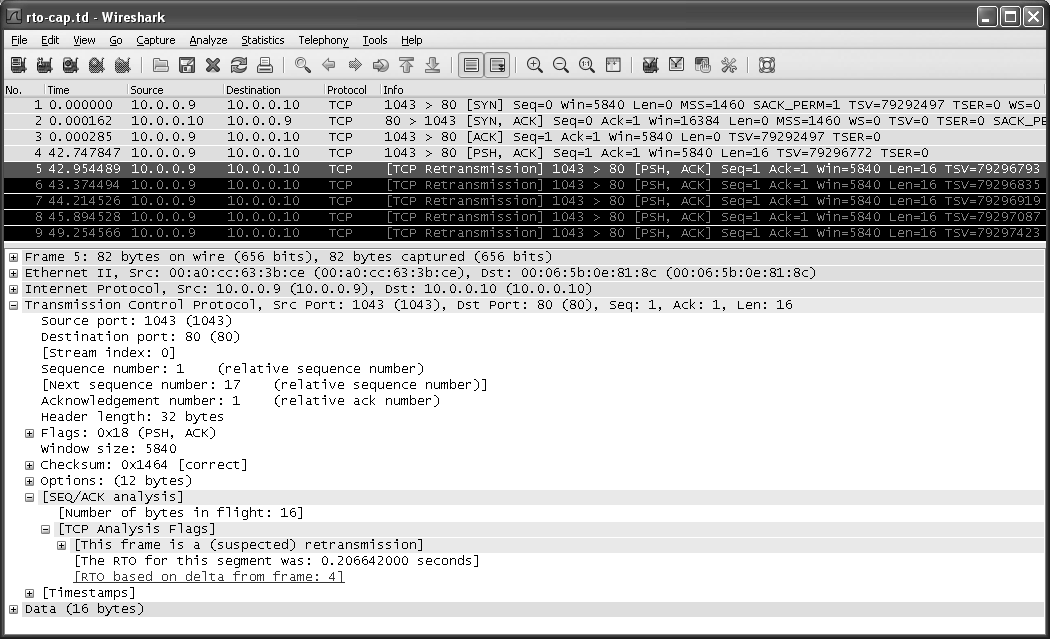
\includegraphics[width=1.0\textwidth]{imgs/14/14-1.png}
	\caption{tcp重传简单的例子}
\end{figure}

报文段1、2、3为TCP建立连接的握手过程。连接建立完成后,Web 服务器处于等待 Web 请求的状态。在发出请求前,我们先断开服务器端主机的连接。在客户端输入如下命令:
\begin{verbatim}
    Linux% telnet 10.0.0.10 80
    Trying 10.0.0.10...
    Connected to 10.0.0.10.
    Escape character is '^]'.
    GET / HTTP /1.0
    Connection closed by foreign host.
\end{verbatim}

该请求无法传输至服务器端,因此它会在客户端的TCP 队列中存储一段时间。此时采用 netstat 命令读取客户端队列状态显示为非空:

\begin{verbatim}
Active Internet connections (w/o servers)
Proto Recv-Q Send-Q     Local Address       Foreign Address     State
tcp        0     18     10.0.0.9:1043       10.0.0.10:www       ESTABLISHED
\end{verbatim}

可以看到发送队列中有18字节的数据,等待被传送至Web 服务器。这18个字节包含了之前显示的请求命令以及回车换行。其他的输出细节(包括地址和状态信息)会在下面涉及。

报文段4为客户端首次尝试发送 Web 请求,时间为 42.748s。0.206s 以后,在42.9545发送了第二次请求。接着在 43.374S,即 0.420s后,再次尝试请求。后续的请求(重传)时刻
分别为 44.215、45.895以及 49.255s,间隔分别为1.680和 3.360s。

每次重传间隔时间加倍称为\textcolor{red}{二进制指数退避}(binary exponential backoff),我们在第13章的TCP 尝试建立连接失败时提到过,后面将会详细讨论。自首次请求至连接完全失效,
总时间为15.5min。随后,客户端会显示如下错误信息:
\begin{verbatim}
    Connection closed by foreign host.
\end{verbatim}

逻辑上讲,TCP 拥有两个阈值来决定如何重传同一个报文段。主机需求 RFC[RFC1122]描述了这两个阈值,在第13 章中也提到过。R1表示 TCP 在向IP 层传递“消极建议”(如重新
评估当前的I路径)前,愿意尝试重传的次数(或等待时间)。R2(大于R1)指示 TCP 应放弃当前连接的时机。R1 和R2应分别至少设为三次重传和100秒。对连接的建立过程(发送
SYN 报文段),阈值设置与数据段传输有所区别,针对SYN报文段的R2应最少设为3分钟。

Linux 系统中,对一般数据段来说,R1 和 R2的值可以通过应用程序,或使用系统配置变量 \verb|net.ipv4.tcp_retries1| 和 \verb|net.ipv4.tcp_retries2|设置。变量值为重传次数,而不是以时间为
单位。\verb|tcp_retries2|默认值为15,对应约为\(13-30\)分钟,根据具体连接的 RTO而定。\verb|net.ipv4.tcp_retries1| 默认值为3。对于SYN报文段,变量 \verb|net.ipv4.tcp_syn_retries|
和 \verb|net.ipv4.tcp_synack_retries| 限定重传次数,默认值为5(约180秒)。Windows 也有相应控制 TCP行为的变量,包括R1 和 R2。通过下列注册表项可以修改对应值 [WINREG]:

\begin{verbatim}
    HKLM\System\CurrentControlSet\Services\Tcpip\Parameters
    HKLM\System\CurrentControlSet\Services\Tcpip6\Parameters
\end{verbatim}

最主要的值为 TepMaxDataRetransmissions,对应 Linux 中的 \verb|tcp_retries2| 变量,其默认值为5。至此我们看到,TCP 需要为重传计时器设置超时值,指示发送数据后等待ACK的
时间。假设 TCP 只工作在静态环境中,那么很容易为超时设置一个合适的值。由于 TCP 需要适应不同环境进行操作,可能随着时间不断变化,因此需基于当前状态设定超时值。例
如,若某个网络连接失败,需重新建立,RTT也会随之改变(可能变化很大)。也就是说,TCP 需要动态设置 RTO(重传超时)。下面我们讨论这一问题。

\section{设置重传超时}
TCP 超时和重传的基础是怎样根据给定连接的 RTT设置 RTO。若TCP 先于 RTT 开始重传,可能会在网络中引入不必要的重复数据。反之,若延迟至远大于 RTT 的间隔发送重
传数据,整体网络利用率(及单个连接吞吐量)会随之下降。由于 RTT的测量较为复杂,根据路由与网络资源的不同,它会随时间而改变。TCP 必须跟踪这些变化并适时做出调整来维
持好的性能。

TCP 在收到数据后会返回确认信息,因此可在该信息中携带一个字节的数据(采用一个特殊序列号)来测量传输该确认信息所需的时间。每个此类的测量结果称为 RTT 样本(RTT
sample)。TCP 首先需要根据一段时间内的样本值建立好的估计值。第二步是怎样基于估计值设置 RTO。RTO 设置得当是保证TCP 性能的关键。

每个TCP连接的 RTT均独立估算,并且重传计时器会对任何占用序列号的在传数据(包括SYN 和FIN报文段)计时。如何恰当设置计时器一直以来都是研究的热点问题,近年
来也取得了一些成果。本章节将探讨计算 RTO 计算方法在演进历程中的一些重要里程碑。首先我们介绍第一个(“经典”)方法,详见[RFCO793]。

\subsection{经典方法}
最初的 TCP 规范 [\href{https://datatracker.ietf.org/doc/html/rfc0793#section-3.7}{RFC0793}]采用如下公式计算得到平滑的 RTT 估计值(称为 SRTT):
\begin{equation}
    SRTT = \alpha(SRTT) + (1 - \alpha) RTT,
\end{equation}

这里,SRTT 是基于现存值和新的样本值 RTT.得到更新结果的。常量a为平滑因子,推荐值0.8~0.9。每当得到新的样本值,SRTT 就会做出相应的更新。从a的设定值可以看
到,新的估计值有80\% ~90\%来自现存值,10\% ~20\%来自新测量值。这种估算方法称为指数加权移动平均(Exponentially Weighted Moving Average, EWMA)或低通过滤器 (low-
pass filter)。该方法实现起来较为简单,只要保存SRTT 的先前值即可得到新的估计值。

考虑到 SRTT 估计器得到的估计值会随 RTT 而变化,[\href{https://datatracker.ietf.org/doc/html/rfc0793#section-3.7}{RFC0793}] 推荐根据如下公式设置RTO:
\begin{equation}
    RTO = min(ubound, max(lbound, (SRTT)B))
\end{equation}

这里的B为时延离散因子,推荐值为1.3~2.0。ubound为RTO 的上边界(可设定建议值,如1分钟),lbound为 RTO 的下边界(可设定建议值,如1秒)。我们称该方法为经典方法,
它使得 RTO 的值设置为1秒,或约两倍的SRTT。对于相对稳定的RTT分布来说,这种方法能取得不错的性能。然而,若 TCP运行于 RTT 变化较大的网络中,则无法获得期望的效果。

\subsection{标准方法}
在[88]中,Jacobson 进一步分析了上述经典方法,即按照[RFC0793]设置计时器无法适应 RTT 的大规模变动(特别是,当实际的 RTT远大于估计值时,会导致不必要的重传)。
增大的RTT 样本值表明网络已出现过载,此时不必要的重传无疑会进一步加重网络负担。

为解决上述问题,可对原方法做出改进以适应RTT变动较大的情况。可通过记录 RTT测量值的变化情况以及均值来得到较为准确的估计值。基于均值和估计值的变化来设置
RTO,将比仅使用均值的常数倍来计算 RTO更能适应 RTT 变化幅度较大的情况。

[88] 中的图5和图6显示了采用[RFC0793]与同时考虑 RTT变化值的方法计算 RTO的对比情况。如果我们将 TCP 得到的 RTT测量样本值考虑为一个统计过程,那么同时测量
均值和方差(或标准差)能更好地估计将来值。对 RTT的可能值范围做出好的预测可以帮助TCP 设定一个能适应大多数情况的 RTO值。

正如 Jacobson 所述,平均偏差(mean deviation)是对标准差的一种好的逼近,但计算起来却更容易、更快捷。计算标准差需要对方差进行平方根运算,对于快速 TCP 实现来说代
价较大。(但这并非全部原因,可参见[G04] 中所述的有趣的“争论”历史。)因此我们需要结合平均值和平均偏差来进行估算。可对每个 RTT 测量值 M(前面称为 RTT.)采用如下算式:

\begin{equation}
    srtt \leftarrow (1-g)(srtt) + (g)M
\end{equation}
\begin{equation}
    rttvar \leftarrow (1-h)(rttvar) + (h)(|M-srtt|)    
\end{equation}
\begin{equation}
    Rto = srtt + 4(rttvar)
\end{equation}

这里,srt 值替代了之前的SRTT,且rttvar 为平均偏差的EWMA,而非采用先前的B来设置 RTO。这组等式也可以写成另一种形式,对计算机实现来说操作较为方便:
\begin{equation}
    Err = M - srtt
\end{equation}
\begin{equation}
    srtt \leftarrow srtt + g(Err)
\end{equation}
\begin{equation}
    rttvar \leftarrow rttvar + h(|Err| - rttvar)
\end{equation}
\begin{equation}
    RTO = srtt + 4(rttvar)
\end{equation}

如前所述,srtt 为均值的EWMA,rttvar 为绝对误差IBrrl的EWMA。Err 为测量值 M与当前 RTT 估计值 srtt之间的偏差。srtt与 rttvar 均用于计算 RTO 且随时间变化。增量g为新
RTT 样本M占 srtt估计值的权重,取为1/8。增量h为新平均偏差样本(新样本M与当前平均值 srtt 之间的绝对误差)占偏差估计值 rttvar 的权重,取为1/4。当RTT变化时,偏差的增
量越大,RTO增长越快。8和及的值取为2的(负的)多少次方,使得整个计算过程较为简单,对计算机来说只要采用定点整型数的移位和加法操作即可,而无须复杂的乘除法运算。

\begin{tcolorbox}
    标准差公式:
    \begin{equation}
        \sigma = \sqrt\frac{\sum{(X-\mu)^2}}{N}
    \end{equation}
\end{tcolorbox}
比较经典方法与 Jacobson 的计算方法,平均 RTT 的计算过程类似(a等于1减增量g),只是采用的增量不同。另外,Jacobson 同时基于平滑 RTT 和平滑偏差计算RTO,而经典方
法简单采用平滑 RTT 的倍数。这是迄今为止许多 TCP 实现计算 RTO 的方法,并且由于其作为[RFC6298] 的基础,我们称其为标准方法,尽管在[RFC6298]中有一些改进。下面我们就
讨论这个问题。

\subsubsection{时钟粒度与 RTO 边界}

在测量 RTT的过程中,TCP 时钟始终处于运转状态。对初始序列号来说,实际TCP连接的时钟并非从零开始计时,也没有绝对精确的精度。相反地,TCP 时钟通常某个变量,
该变量值随着系统时钟而做出更新,但并非一对一地同步更新。TCP 时钟一个“滴答”的时间长度称为粒度。通常,该值相对较大(约500ms),但近期实现的时钟使用更细的粒度(如
Linux 采用1ms)。

粒度会影响 RTT的测量以及 RTO的设置。在[RFC6298]中,粒度用于优化 RTO 的更新情况,并给RTO设置了一个下界。计算公式如下!

这里的G为计时器粒度,1000ms 为整个 RTO 的下界值([RFC6298] 的规则(2.4)建议值)。因此,RTO 至少为1s,同时提供了可选上界值,假设为60s。

\subsubsection{初始值}

我们已经看到估计器怎样随时间进行更新,但同时也需要了解怎样设置初始值。在首个SYN 交换前,TCP 无法设置 RTO 初始值。除非系统提供(有些系统在转发表中级存了该信
息,见14.9节),否则也无法设置估计器的初始值。根据[RFC6298],RTO 的初始值为1s,而初始 SYN 报文段采用的超时间隔为3s。当接收到首个 RTT 测量结果M,估计器按如下方
法进行初始化:

\begin{equation}
    srtt +- M
    rttvar ‹- M/2
\end{equation}

我们已经了解了估计器的初始化和运行过程。RTO 的设置看似取决于得到的RTT采样值,下面我们将看到一些例外情况。
\subsubsection{重传二义性与Karn 算法}

在测量 RTT样本的过程中若出现重传,就可能导致某些问题。假这一个包的传输出现超时,该数据包会被重传,接着收到一个确认信息。那么该信息是对第一次还是第二次传输
的确认就存在二义性。这就是重传二义性的一个例子。

[KP87]指出,当出现超时重传时,接收到重传数据的确认信息时不能更新 RTT 估计值。这是 Kar 算法的“第一部分”。它通过排除二义性数据来解决 RTT估算中出现的二义性问
题。[RFC6298] 做出了相关要求。

假如我们在设置 RTO 过程中简单地将重传问题完全忽略,就可能将网络提供的一些有用信息也同时忽略(即网络中可能出现某些因素影响传输速度)。这种情况下,在网络不
再出现丢包前降低重传率有助于减轻网络负担。这也是下面指数退避行为的理论基础,见图14-1。

TCP 在计算 RTO 过程中采用一个退避系数(backoff factor),每当重传计时器出现超时,退避系数加倍,该过程一直持续至接收到非重传数据。此时,退避系数重新设为1(即二进
制指数退避取消),重传计时器返回正常值。对重传过程退避系数加倍,这是Kar 算法的“第二部分”。注意若 TCP 超时,同时会引发拥塞控制机制,以此改变发送速率(拥塞控制
将在第16 章详细讨论)。因此,Kam 算法实际上由两部分组成,如[KP89]所述:

当接收到重复传输(即至少重传一次)数据的确认信息时,不进行该数据包的RTT测量,可以避免重传二义性问题。另外,对该数据之后的包采取退避策略。仅
当接收到未经重传的数据时,该 SRTT 才用于计算 RTO。

Kam 算法一直作为 TCP 实现中的必要方法(自『RFC1122]起),然而也有例外情况。在使用 TCP 时间戳选项(见第13章)的情况下,可以避免二义性问题,因此Karn 算法的第-
部分不适用。

\subsubsection{带时间戳选项的 RTT测量}

TCP 时间戳选项(TSOPT)作PAWS算法的基础(第13章中已经提过),还可用作RTT 测量(RTTM)[RFC1323]。TSOPT 的基本格式第13 章中已经介绍过。它允许发送者在
返回的对应确认信息中携带一个32比特的数。

时间戳值(TSV)携带于初始SYN的 TSOPT 中,并在 SYN +ACK 的 TSOPT的 TSER部分返回,以此设定srtt、rttvar 与 RTO 的初始值。由于初始SYN 可看作数据(即同样采取
丢失重传策略且占用一个序列号),应测量其 RTT值。其他报文段中也包含 ISOPT,因此可结合其他样本值估算该连接的RTT。该过程看似简单但实际存在很多不确定因素,因为TCP
并非对其接收到的每个报文段都返回 ACK。例如,当传输大批量数据时,TCP 通常采取每两个报文段返回一个 ACK 的方法(见第15章)。另外,当数据出现丢失、失序或重传成功
时,TCP 的累积确认机制表明报文段与其 ACK之间并非严格的一一对应关系。为解决这些问题,使用时间戳选项的 TCP(大部分的 Linux 和 Windows 版本都包含)采用如下算法来测
量 RTT样本值:
\begin{enumerate}
    \item TCP 发送端在其发送的每个报文段的 TSOPT的TSV 部分携带一个32比特的时间戳值。该值包含数据发送时刻的 TCP 时钟值。
    \item 接收端记录接收到的 TSV 值(名为 TsRecent 的变量)并在对应的ACK 中返回,并且记录其上一个发送的 ACK 号(名 LastACK的变量)。回忆一下,ACK 号代表接收端(即ACK 的发送方)期望接收的下一个有序序号。
    \item 当一个新的报文段到达时,如果其序列号与LastACK 的值吻合(即为下一个期望接收的报文段),则将其 TSV 值存人 TsRecent。
    \item 接收端发送的任何一个 ACK 都包含 TSOPT,TsRecent 变量包含的时间戳值被写人其TSER部分。
    \item 发送端接收到 ACK 后,将当前 TCP 时钟减去 TSER 值,得到的差即为新的RTT样本估计值。
\end{enumerate}
FreeBSD、Linux 以及近期的Windows版本都默认启用时间戳选项。在Linux 中,系统配置变量 \verb|net.ipv4.top_timestamps|控制是否使用该选项(0代表禁用,1代表使用)。在
Windows 中,通过前面提到的注册表区域的 Tep13230pts 值来控制其使用。若值0,时间戳被禁用;若值为2,则启用。该键值没有设默认值(它并非默认存在于注册表中)。但若在
连接初始化过程中,TCP通信的另一方使用时间戳,则默认启用。

\subsection{Linux 采用的方法}

Linux 的RTT 测量过程与标准方法有所差别。它采用的时钟粒度为1ms,与其他实现方法相比,其粒度更细,TSOPT也是如此。采用更频繁的 RTT 测量与更细的时钟粒度,RTT测
量也更为精确,但也易于导致 rttvar 值随时间减为最小[LS00]。这是由于当累积了大量的平均偏差样本时,这些样本之间易产生相互抵消的效果。这是其 RTO 设置区别于标准方法的一
个原因。另外,当某个 RTT样本显著低于现有的 RTT估计值 srtt 时,标准方法会增大 rttvar。

为更好地理解第二个问题,首先回顾一下 RTO通常设置为 srtt +4(rttvar)。因此,无论最大 RTT 样本值是大于还是小于 srtt,rttvar 的任何大的变动都会导致 RTO增大。这与直觉
相反——若实际 RTT 大幅降低,RTO并不会因此增大。Linux 通过减小 RTT样本值大幅下降对 rttvar 的影响来解决这一问题。下面我们详细讨论Linux设置 RTO 的方法,该方法可以
同时解决上述两个问题。

与标准方法一样,Linux 也记录变量 srt 与 rttvar 值,但同时还记录两个新的变量,即mder 和\verb|mdev_max|。mdev 为采用标准方法的瞬时平均偏差估计值,即前面方法的rttvar。
\verb|mdev_max|则记录在测量 RTT 样本过程中的最大 mdev,其最小值不小于 50ms。另外,rttvar需定期更新以保证其不小于 \verb|mdev_max|。因此 RTO 不会小于 200ms。

注意 最小 RTO可更改,这可通过在重新编译加载内核前改变內核配置常量\verb|TCP_RTO_MIIN| 的值来实现。有些Linux版本也允许通过ip route 命令改变该值。若
在数据中心网络中使用TCP,这些环境中RTT可能只有几微秒。当本地交换出现丟色时,若RTO的最小值力200ms,就会严重影响网络性能。这就是所谓的
TCP“添头”问题。针对这一问题提出了很多解决方法,包接调整TCP时钟粒度;或将最小RTO 设内几微秒IVO9],但不推荐在全球固特网中使用该方法。

Linux 根据 \verb|mdev_max|的值来更新 rttvar。 RTO 总是等于 srt 与4(rttvar)之和,以此确保RTO 不超过\verb|TCP_RTO_MAX|(歡认值为120s)。详见[SK02]。图14-2 详细描述了这一过程,
从中也可看到时间戳选项是怎样工作的。

TCP 时间戳选项携带了发送端 TCP 时钟的副本。接着 ACK 将该值返回至接收端,通过计算两者之差(当前时钟减去返回的时间戳)来更新其 srt 与 rttvar 估计值。为看得更清晰,图中
只描述了一部分时间戳。本 Linux 系统中,rttvar 值限制为至少50ms,RTO 下界值为200ms

从图14-2中可以看到,该TCP 连接采用时间戳选项。发送端为 Linux 2.6 系统,接收端为 FreeBSD 5.4 系统。为简单起见,序列号和时间戳取相对值,且只显示了发送端的时间
戳。为使数据简单可读,本图并未严格按照时间尺度。基于本例中得到的初始 RTT 测量值,Linux 采用如下算法进行更新:
\begin{itemize}
    \item srtt = 16ms
    \item mdev = (16/2)ms = 8ms
    \item rttvar = \verb|mdev_max| = maxmdev, \verb|TCP_RTO_MIN|) = max(8, 50) = 50ms
    \item RTO = srtt + 4(rttvar)=16+4(50) =216ms
\end{itemize}

在初始SYN 交换后,发送端对接收端的 SYN返回一个 ACK,接收端则进行了一次相应的窗口更新。由于这些包都未包含实际数据(SYN或 FIN位字段,但都被算作数据),并
没有记录对应的时间,且发送端收到窗口更新时也没有进行 RTT更新。TCP 对不含数据的报文段不提供可靠传输,意味着若出现丢包不会重传,因此无须设定重传计时器。

值得注意的是,TCP选项本身并不进行重传或可靠传输。仅当数据段(包括SYN 和FIN报文段)中明确设定,才会丢失重传,但也仅作副作用。

当应用首次执行写操作,发送端 TCP发送两个报文段,每个报文段包含一个值为127的TSV。由于两次发送间隔小于1ms(发送端TCP 时钟粒度),因此这两个值相等。当发送
端以这种方式接连发送多个报文段时,很容易看到时钟没有前进或小幅前进的情况。

接收端变量 LastACK记录其上一个发送ACK 的序列号。在本例中,上一个发送的ACK 为连接建立阶段的SYN +ACK 包,因此 LastACK 从1开始。当首个全长(full-size)
报文段到达,其序列号与LastACK 吻合,则将 TsRecent 变量更新为新接收分组的TSV,即127。第二个报文段的到达并没有更新 TsRecent,因其序列号字段与LastACK 中的值并不
匹配。接收端返回对应分组的ACK 时,需在其 TSER 部分包含 TsRecent,同时接收端还要更新 LastACK 变量的ACK 号为2801。

当该ACK 到达时,TCP 就可以进行第二个 RTT样本的测量。首先获得当前 TCP 时钟值,减去已接收 ACK 包含的 TSER,即样本值 m=223-127=96。根据该测量值,Linux
TCP 按如下步骤更新连接变量:

\begin{itemize}
    \item \verb|mdev = mdev (3/4) + m - srtt| (1/4) = 8(3/4) + 80|1/4) = 26ms|
    \item \verb|mdev_max = max(mdev_max, mdev) = max(50, 26) = 50ms|
    \item srtt = srtt (7/8) +m(1/8) =16(7/8) +96(1/8)=14+12=26ms
    \item rttvar = mdev max = 50ms
    \item RTO = srtt + 4(rttvar) = 26 + 4(50) = 226ms
\end{itemize}

如前所述,Linux TCP 针对经典 RTT估算方法做出了几处改进。在经典算法提出之时,TCP 时钟粒度普遍为500ms,且时间戳选项也没有得到广泛应用。通常,每个窗口只测量一
个 RTT样本,并据此进行估计器的更新。在不使用时间戳的情况下,依然采用这种方法。

若每个窗口只测量一个 RTT样本,rtvar 相对变动则较小。利用时间戳和对每个包的测量,就可以得到更多的样本值。因为对同一个窗口的数据而言,每个包对应的RTT样本通
常存在一定的差异,短时间内得到的大量样本值(如窗口较大)可能导致平均偏差变小(接近0,基于大数定律[F68])。为解决上述问题,Linux 维护瞬时平均偏差估计值 mdev,但设
置 RTO 时则基于 rttvar(在一个窗口数据期间记录的最大 mdev,且最小值50ms)。仅当进入下一个窗口时,rttvar 才可能减小。

标准方法中 rttvar 所占权重较大(系数为4),因此即使当 RTT 减小时,也会导致 RTO增长。在时钟粒度较粗时(如500ms),这种情况不会有很大影响,因为 RTO 可用值很少。
然而,若时钟粒度较细,如Linux的1ms,就可能出现问题。针对 RTT 减小的情况,若新样本值小于 RTT估计范围的下界(srtt -mdev),则减小新样本的权重。完整的关系式如下:

\begin{lstlisting}[]
if (m < (stt - mdev))
    mdev = (31/32) * mdev + (1/32) * |srtt - m|
else
    mdev = (3/4) * mdev + (1/4) * |srtt -mn|
\end{lstlisting}

该条件语句只在新 RTT样本值小于期望的RTT测量范围下界的前提下成立。若该条件成立,则表明该连接的 RTT 正处于急剧减小的状态。为避免该情况下的 mdev 增大(以及由
此导致的 rttvar 和RTO增大),新的平均偏差样本 Isrtt-ml,将其权重减小为原来的1/8。整体来看,该结果可以避免 RTT减小导致的RTO增大问题。对该问题的进一步讨论,请参见
[LS00]及[SK02]。在[RKS07]中,作者在280万个 TCP流的多个系统上运行了 RTT 估算算法,运行结果表明 Linux 估计器性能最优,这很大程度上是由于其相对快速收敛,但也可能
是减小了 RTT 变动对 RTO 的影响。

\begin{figure}[!htb]
    \centering
	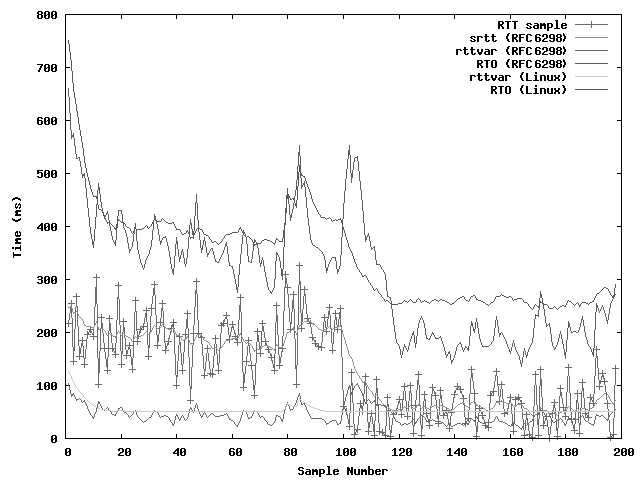
\includegraphics[width=0.7\textwidth]{imgs/14/14-3.png}
	\caption{对于200个伪随机的样本点采用 Linux 方法和标准方法来设置 RTO 和估算 RTT。前100个点是基于分布 N(200,50),后100个则基于N(50,50),且对负值进行了符号变换。Linux 将最小
    RTO设为200ms,而标准方法在样本120之后则变得更为密集。Linux 避免 RTO 设置过小就是防止这种情况的发生。标准方法在样本 78 和191 出现潜在问题}
\end{figure}

现在回到图 14-2,当接收端生成 ACK 7001时,我们看到其 TSER 包含了一个 TSV 副本,该值并非来自最新到达的报文段,而是最早的一个未经确认的报文段。当该ACK 返回
至发送端,通过计算得到的 RTT样本是基于第一个报文段,而非第二个。这说明了时间戳算法在延时或不稳定的ACK 下的工作情况。若计算最早的包对应的RTT,得到的样本值为
发送端期望收到 ACK 需经过的时间,而非实际网络 RTT。这点很重要,因为发送端需根据其ACK 接收率来设置 RTO,接收率可能小于包的发送率。

\subsection{RTT 估计器行为}
我们已经看到,设置 RTO 与估算 RTT有大量的设计和改进方法。图14-3显示了其中主要的估算方法,即基于标准方法和 Linux 算法得到的综合数据集。图中[RFC6298] 推荐的标
准算法最小 RTO 值1s 已被移除。目前的大多数 TCP 实现方法都不再采用该值[RKS07]。

图中显示了两个在高斯概率分布 N(200,50) 和 N(50,50)上的200个值对应的时间序列图。第一个分布对应前100个点,第二个对应后100个点。负的样本值通过符号变换转化为
正值(只针对第二个分布)。每个加号(+)表示一个具体的样本值。很明显可以看到,在第100个样本值之后出现了巨幅下降,另外 Linux 方法在第100个样本值之后 RTO 立即减小,
而标准方法则在120个样本值后才开始减小。

观察 Linux 的 rttvar线,可以看到其基本保持恒定。这是由于 \verb|mdev_max| 的最小值力50ms(因此 rtvar 也是如此),使得 Linux 的RTO 始终保持在200ms 以上,并且避免了所有
不必要的重传(尽管可能由于 RTO 较大,计时器未超时,导致丢包时性能降低)。标准方法在样本78和191 可能出现潜在问题,即伪重传的发生。这个问题留到后面再讨论。

\subsection{RTTM 对丟包和失序的鲁棒性}

当没有丢包情况时,不论接收端是否延迟发送ACK,TSOPT 可以很好地工作。该算法在以下几种情况下都能正确运行:
\begin{itemize}
    \item 失序报文段:当接收端收到失序报文段时,通常是由于在此之前出现了丢包,应当立即返回 ACK 以启动快速重传算法(见14.5节)。该ACK的TSER 部分包含的 TSV值为接收端收到最近的有序报文段的时刻(即最新的使窗口前进的报文段,通常不会是失序报文段)。这会使得发送端RTT样本增大,由此导致相应的RTO增大。这在一定程度上是有利的,即当包失序时,发送端有更多的时间去发现是出现了失序而非丢包,由此可避免不必要的重传。
    \item 成功重传:当收到接收端缓存中缺失的报文段时(如成功接收重传报文段),窗口通常会前移。此时对应 ACK 中的TSV 值来自最新到达的报文段,这是比较有利的。若采用原来报文段中的TSV,可能对应的是前一个 RTO,导致发送端 RTT 估算的偏离。
\end{itemize}

图14-4的例于描述了这些点。假设三个报文段,每个包含1024字节,接收顺序如下:报文段1包含1~1024字节,报文段3包含2049~3027字节,接着是报文段2包含1025~2048字节。

当报文段失序,返回的时间戳为最新的使窗口前移的报文段(而非到达接收端的最大的时间微)。这将使得发送端 RTO 在包失序期间过高估计 RTT,并降低其重传积极性

图14-4中发回的ACK 1025 包含了报文段1的时间戳(正常的数据确认),以及另一个包含报文段1时间戳的ACK 1025(对应于在窗口中但失序的重复 ACK),接着是 ACK 3037
包含了报文段2的时间戳(而非报文段3的时间戳)。当分组失序(或丢失)时,RTT会被过高估算。较大的 RTT 估计值使得 RTO也更大,由此发送端也不会急于重传。在失序情况下
这是很有利的,因为过分积极的重传可能导致伪重传。

我们已经看到,时间戳选项使得发送端即使在丢包、延时、失序的情况下也能测量RTT。发送端在测量 RTT 的过程中,可以在其选项中包含任意值,但其单位必须至少和实
际时间成比例,且粒度合理,并与TCP 序列号兼容,连接速率可信(详见[RFC1323])。特别是,为了对发送端更有利,对任何可信的 RTT,TCP 时钟必须至少“滴答”一次。另外,
其每次变化不能快于59ns。若小于,在IP 层允许单个包存在的最大时间(255s)内,记录TCP 时钟的32位的 TSV 值能够环绕[ID1323b]。满足上述所有条件后,RTO值就可以用来
触发重传。

\section{基于计时器的重传}
一旦 TCP发送端得到了基于时间变化的 RTT测量值,就能据此设置RTO,发送报文段时应确保重传计时器设置合理。在设定计时器前,需记录被计时的报文段序列号,若及时收
到了该报文段的ACK,那么计时器被取消。之后发送端发送一个新的数据包时,需设定一个新的计时器,并记录新的序列号。因此每一个 TCP 连接的发送端不断地设定和取消一个
重传计时器;如果没有数据丢失,则不会出现计时器超时。

\begin{tcolorbox}
    该过程对主机操作系统设计者来说可能难以理解。对典型的操作系统来说,计时器用于标记大量事件,计时器的实现也仅限于有效地设定和触发超时(需要调
    用系统函数)。然而对TCP 来说,计时器需要有效地实现被设置、重新设置或取消的功能;若TCP正常工作,则计时器不会出现超时的情况。
\end{tcolorbox}

若在连接设定的RTO 内,TCP没有收到被计时报文段的ACK,将会触发超时重传。我们已经在图14-1中看到这一过程。TCP 将超时重传视为相当重要的事件,当发生这种情况
时,它通过降低当前数据发送率来对此进行快速响应。实现它有两种方法:第一种方法是基于拥塞控制机制减小发送窗口大小(见第16章);另一种方法为每当一个重传报文段被再次
重传时,则增大RTO 的退避因子,即前面提到的Kar 算法的“第二部分”。特别是当同一报文段出现多次重传时,RTO 值(暂时性地)乘上值y来形成新的超时退避值:
\begin{equation}
RTO = yRTO
\end{equation}

在通常环境下,»值为1。随着多次重传,》呈加倍增长:2,4,8,等等。通常y不能超过最大退避因子(Linux 确保其 RTO 设置不能超过 \verb|TCP_RTO_MAX|,其默认值为120s)。
一旦接收到相应的ACK,》会重置为1。

\subsection{例子}

我们通过建立一个与图14-1 和图14-2相似的连接来观察重传计时器的行为。这里故意两次将序列号为 1401 的报文段丢弃(见图14-5)。

在本例中,我们可以利用一个特殊函数将某个序列号的报文段多次丢弃。这与图14-2相比,将会使 RTT引入一定的延时。连接建立之初与之前类似,仅当发送序列号为1和
1401 的报文段时,后一个包才被丢弃。当一个报文段到达接收端时,接收端并没有立即给出响应而是延迟发送ACK。在219ms 内都没有得到回应,发送端的计时器超时,导致序列号
为1的包被重传(此时的 TSV 值力577)。随即该包的到达使得接收端返回一个ACK。由于该 ACK 确认了数据被成功接收,并使得窗口前移,其TSER 值被用于更新 srtt 和 RTO 分别
为34 和234。

接着返回了三个 ACK,带星号(*)的ACK为重复ACK,但含了SACK 信息。我们将在14.5节和14.6节讨论重复ACK 和SACK。现在,由于这些ACK并没有使发送窗曰前移,
这些 TSER 值不会被采用。

随着最后一次重传以及报文段1401 到达(在TCP 时钟为911的时刻),修复阶段完成,接收端返回序列号为7001的ACK,表明所有数据已成功接收。

当网络无法正常传输数据时,重传计时器为 TCP 连接提供了“最后一招的重新启动”。在大多数情况下,计时器超时并触发重传是不必要的(也不是期望的),因为RTO的政路通
常大于 RTT(约2倍或更大),因此基于计时器的重传会导致网络利用率的下降。幸运的是,TCP 有另一种方法来检测和修复丢包,它比超时重传更为高效。由于它并不需要计时器超时
来触发,因此称为快速重传。

\section{快速重传}
快速重传机制[RFC5681]基于接收端的反馈信息来引发重传,而非重传计时器的超时。因此与超时重传相比,快速重传能更加及时有效地修复丢包情况。典型的TCP 同时实现了
两者。在详细讨论快速重传前,首先需要了解当接收到失序报文段时,TCP 需要立即生成确认信息(重复 ACK),并且失序情况表明在后续数据到达前出现了丢段,即接收端级存出现
了空觖。发送端的工作即为尽快地、高效地填补该空映。

当失序数据到达时,重复ACK应立即返回,不能延时发送。原因在于使发送端尽早得知有失序报文段,并告诉其空缺在哪。当采用SACK 时,重复ACK 通常也包含SACK 信
息,利用该信息可以获知多个空峡。

重复 ACK(不论是否包含SACK 信息)到达发送端表明先前发送的某个分组已丢失。在14.8节中我们会更详细地讨论到,重复 ACK 也可能在另一种情况下出现,即当网络中出现
失序分组时——若接收端收到当前期盼序列号的后续分组时,当前期盼的包可能丢失,也可能仅为延迟到达。通常我们无法得知是哪种情况,因此TCP 等待一定数目的重复ACK(称
为重复 ACK 网位或 dupthresh),来决定数据是否丢失并触发快速重传。通常,dupthresh 为常量(值为3),但一些非标准化的实现方法(包括Linux)可基于当前的失序程度动态调节
该值(见14.8节)。

快速重传算法可以概括如下:TCP 发送端在观测到至少 dupthresh 个重复ACK 后,即重传可能丢失的数据分组,而不必等到重传计时器超时。当然也可以同时发送新的数据。根据
重复 ACK 推断的丢包通常与网络拥塞有关,因此伴随快速重传应触发拥塞控制机制(详见第16章)。不采用SACK 时,在接收到有效ACK 前至多只能重传一个报文段。采用SACK,
ACK 可包含额外信息,使得发送端在每个 RTT 时间内可以填补多个空映。在描述一个基本快速重传算法的例子之后,我们将讨论快速重传中SACK 的用法。

\subsection{例子}
在下面的例子中,我们建立一个与图14-4类似的连接,但这次丢奔报文段23801 和26601,并且禁用SACK。我们将看到 TCP怎样利用基本的快速重传算法来填补空缺。发送
端为 Linux 2.6 系统,接收端为 FreeBSD 5.4 系统。图14-6可通过 Wireshark 的“统计ITCP流图| 时间序列图”(Statistics | TCP Stream Graph | Time-Sequence Graph)功能(toptrace)得
到,该图显示了快速重传行为。


\begin{figure}[!htb]
	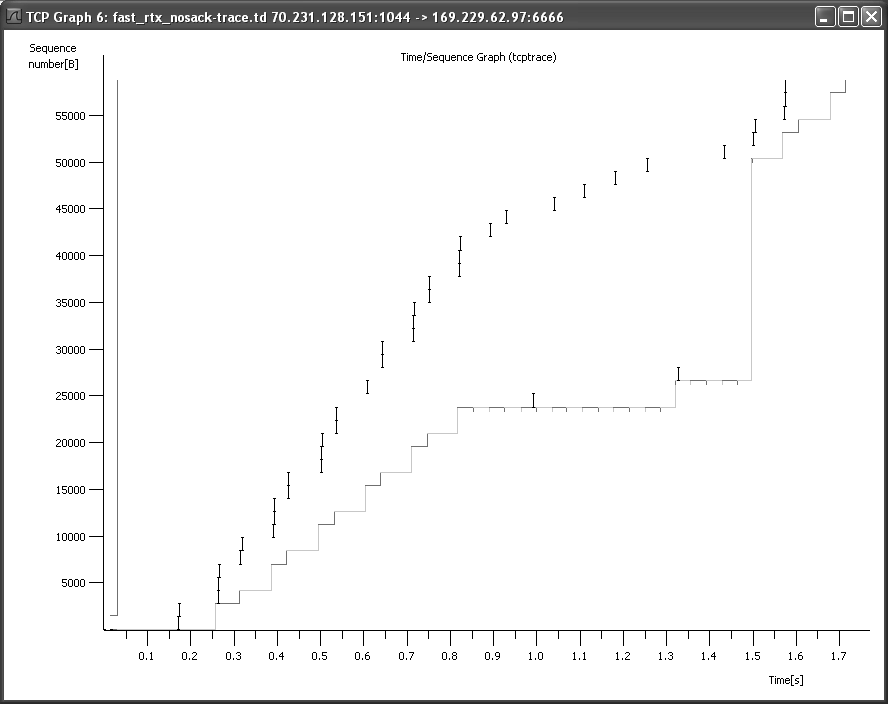
\includegraphics[width=1.0\textwidth]{imgs/14/14-6.png}
	\caption{本图中, 轴为TCP序列号,x轴为时间。发出的报文段用较深的黑色线段标出,收到的ACK 号用浅灰线。在0.993s到达的第三个重复 ACK 触发快速重传。该连接未采用SACK,所以每个 RTT 内至多只能填补一个空缺。
    之后到达的重复ACK 使得发送端发送新报文段(非重传报文段)。在1.32s 时刻到达的“部分ACK”再次触发了重传}
\end{figure}


该图y轴表示相对发送序列号,x轴表示时间。黑色的I形线段表示传输报文段的序列号范围。Wireshark 中的蓝色(图14-6中的浅灰色)线段为返回的ACK号。约1.0s时刻,序
列号 23801发生了快速重传(初始传输不可见,因为被发送端 TCP 下层丢弃)。第三个重复ACK 的到达触发了快速重传,图中表现为重叠的浅灰色线段。通过 Wireshark 的基本分析窗
口也可以观察到重传过程(见图14-7)。

图14-7的第一行(40号)为ACK 23801首次到达。Wireshark 标示出了(红色,在图14-7中看来是黑色)其他“有趣的”TCP 包。这些包与其他没有丢失或异常的包不同。我
们可以看到窗口更新、重复 ACK 和重传。0.853s时刻的窗口更新为带重复序列号的ACK(因为没有携带数据),但包含了 TCP 流控窗口的变动。窗口由231616字节变为233016字节。
因此,它并没有等到三个重复 ACK 来触发快速重传。窗口更新仅是提供了窗口通告的一个副本。我们将在第15 章中详细讨论。

0.8908、0.9268 以及 0.964s时刻到达的均为序列号为23801 的重复ACK。第三个重复ACK 的到达触发了报文段23801的快速重传,时间为0.993S。该过程也可通过 Witreshark 的
“统计|流图”(Statistics | Flow Graph)功能来观测(见图14-8)。

\begin{figure}[!htb]
	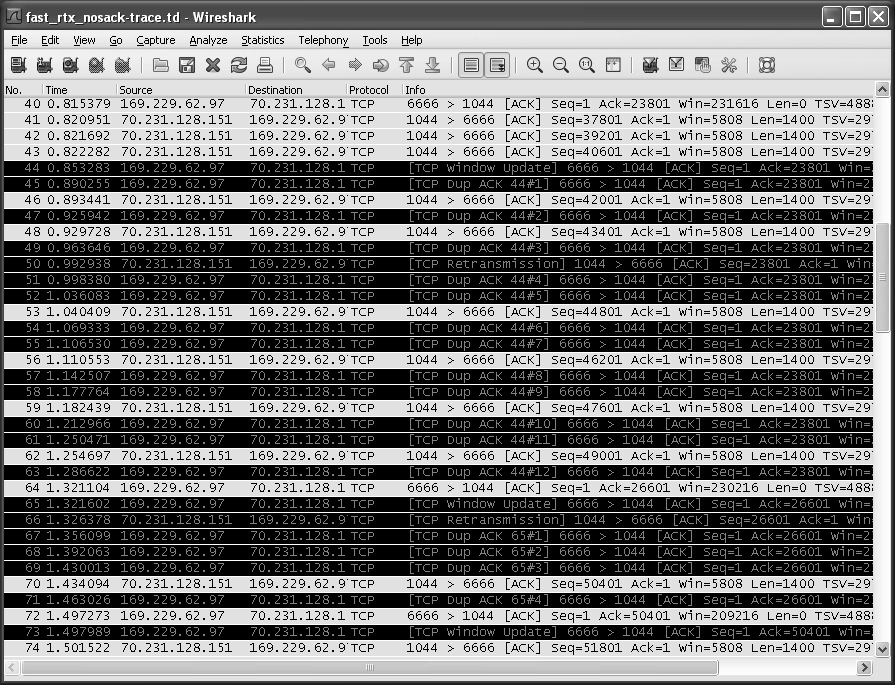
\includegraphics[width=1.0\textwidth]{imgs/14/14-7.png}
	\caption{TCP 交换的相对序列号。包50和66为重传。包50是由三次重复ACK 引发的快速重传。由于没有重传计时器超时,所以恢复过程相对较快}
\end{figure}

现在我们换个角度来看0.993s 时刻的快速重传过程,也可以看1.326s时刻发生的第二次快速重传,该重传是由1.322s时刻达到的ACK 触发的。

第二次重传与第一次有所不同。当第一次重传发生时,发送端在执行重传前已发送的最大序列号为(43401 +1400=44801),称恢复点(recovery point)。TCP 在接收到序列
号等于或大于恢复点的ACK 时,才会被认为从重传中恢复。本例中,1.322s 和1.321s时刻的ACK 并不是44801,而是26601。该序列号大于之前接收到的最大ACK 值(23801),但
不足以到达恢复点(44801)。因此这种类型的ACK 称为部分 ACK (partial ACK)。当部分ACK到达时,TCP 发送端立即发送可能丢失的报文段(这里是26601),并且维持这一过程
直到到达或超过恢复点。如果拥塞控制机制允许(见第16章),也可以同时发送新的数据。

这里的例子并没有采用SACK,不论是快速重传,还是基于“NewReno”算法[RFC3782] 恢复阶段执行的其他重传。由于没有SACK,通过观察返回的ACK 号的增长情
况,发送端在每个 RTT 内只能获知至多一个空缺。

在恢复阶段的具体行为根据 TCP发送端和接收端的类型和配置差异有所不同。这里描述的是无 SACK 发送端采用NewReno算法的例子,这种配置比较常见。根据NewReno算
法,部分ACK 只能使发送端继续处于恢复状态。对较旧的TCP 版本(单纯的Reno 算法)来说,没有部分ACK 这个概念,任何一个可接受的ACK(序列号大于之前接收到的所有
ACK)都能使发送端结束恢复阶段。这种方法可能会使 TCP 出现一些性能问题,我们在第16章会详细讨论。下面讨论 NewReno和SACK,它们有时也被称为“高级丢失恢复”技术,
以此来区别旧的方法。
\begin{figure}[!htb]
    \centering
	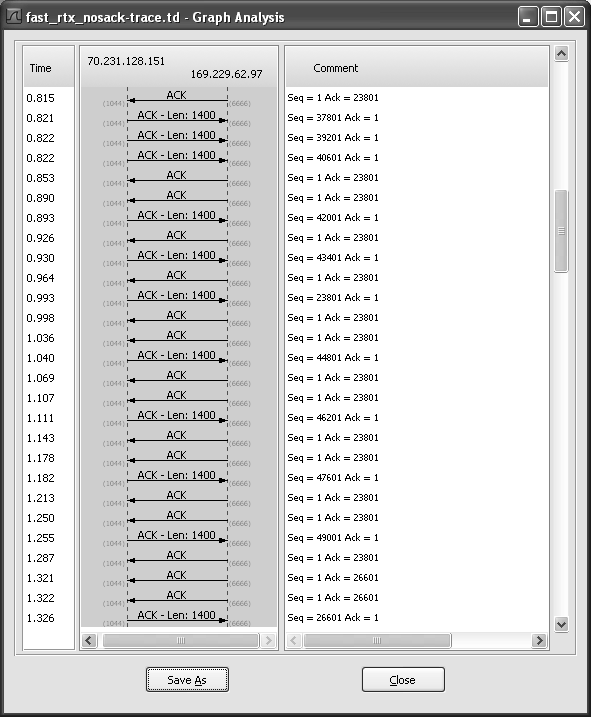
\includegraphics[width=0.5\textwidth]{imgs/14/14-8.png}
	\caption{0.890s、0.926s以及 0.964s 时刻到达的三次重复ACK 触发了0.993s 时刻的快速重传。0.853s时刻的ACK 并不算作重复ACK,因力它包含了一个窗口更新}
\end{figure}

\section{带选择确认的重传}

随着选择确认选项的标准化[RFC2018],TCP 接收端可提供SACK 功能,通过TCP头部的累积 ACK 号字段来描述其接收到的数据。之前提到过,ACK 号与接收端缓存中的其他
数据之间的间隔称为空缺。序列号高于空缺的数据称为失序数据,因为这些数据和之前接收的序列号不连续。

TCP发送端的任务是通过重传丢失的数据来填补接收端缓存中的空缺,但同时也要尽可能保证不重传已正确接收到的数据。在很多环境下,合理采用SACK 信息能更快地实现空缺
填补,且能减少不必要的重传,原因在于其在一个 RTT 内能获知多个空缺。当采用SACK选项时,一个 ACK 可包含三四个告知失序数据的SACK信息。每个 SACK 信息包含32位
的序列号,代表接收端存储的失序数据的起始至最后一个序列号(加1)。

SACK 选项指定n个块的长度为8n +2字节,因此40字节可包含最多4个块。通常SACK 会与TSOPT 一同使用,因此需要额外的10个字节(外加2字节的填充数据),这意味
着SACK 在每个 ACK 中只能包含3个块。

3个块表明可向发送端报告3个空缺。若不受拥塞控制(见第16章)限制,利用SACK选项可在一个 RTT 时间填补3个空映。包含一个或多个SACK块的ACK 有时也简单称为“SACK"。

\subsection{SACK 接收端行为}
接收端在 TCP 连接建立期间(见第13章)收到SACK许可选项即可生成SACK。通常来说,每当缓存中存在失序数据时,接收端就可生成SACK。导致数据失序的原因可能是由
于传输过程中丢失,也可能是新数据先于旧数据到达。这里只讨论第一种情况,后一种留待以后再讨论。

第一个 SACK 块内包含的是最近接收到的(most recently received) 报文段的序列号范围。由于SACK 选项的空间有限,应尽可能确保向TCP发送端提供最新信息。其余的
SACK 块包含的内容也按照接收的先后依次排列。也就是说,最新一个块中包含的内容除了包含最近接收的序列号信息,还需重复之前的SACK 块(在其他报文段中)。

在一个 SACK 选项中包含多个 SACK块,并且在多个 SACK 中重复这些块信息的目的在于,为防止SACK 丢失提供一些备份。若SACK 不会丢失,[RFC2018]指出每个 SACK
中包含一个SACK块即可实现 SACK 的全部功能。不幸的是,SACK 和普通的ACK 有时会丢失,并且若其中不包含数据(SYN或FIN 控制位字段不被置位)就不会被重传。

\subsection{SACK发送端行为}
尽管一个支持SACK 的接收端可通过生成合适的SACK 信息来充分利用SACK,但还不足以使该TCP 连接充分利用SACK 功能。在发送端也应提供SACK 功能,并且合理地利
用接收到的SACK 块来进行丢失重传,该过程也称为选择性重传(selective retransmission)或选择性重发(selective repeat)。SACK 发送端记录接收到的累积 ACK 信息(像大多数 TCP
发送端一样),还需记录接收到的SACK 信息,并利用该信息来避免重传正确接收的数据。一种方法是当接收到相应序列号范围的ACK 时,则在其重传缓存中标记该报文段的选择重传成功。

当SACK 发送端执行重传时,通常是由于其收到了 SACK 或重复ACK,它可以选择发送新数据或重传旧数据。SACK 信息提供接收端数据的序列号范围,因此发送端可据此推断
需要重传的空缺数据。最简单的方法是使发送端首先填补接收端的空缺,然后再继续发送新数据『RFC3517](若拥塞控制机制允许)。这也是最常用的方法。

该行为有一个例外。在[RFC2018] 中,SACK 选项和SACK块的当前规范是建议性的(advisory)。这意味着接收端可能提供一个 SACK 告诉发送端已成功接收一定序列号范围的
数据,而之后做出变更(“食言”)。由于这个原因,SACK 发送端不能在收到一个 SACK后立即清空其重传缓存中的数据;只有当接收端的普通TCP ACK 号大于其最大序列号值时才
可清除。这一规则同样影响重传计时器超时的行为。当TCP 发送端启动基于计时器的重传时,应忽略SACK 显示的任何关于接收端数据失序的信息。如果接收端仍存在失序数据,那
么重传报文段的ACK 中就包含附加的SACK 块,以便发送者使用。幸运的是,食言情况很少出现,也应尽量避免出现。

\subsection{例子}
为理解SACK怎样影响发送端和接收端的行为,我们重复前面的快速重传实验,参数设置也如前(丢掉序列号 23601 与28801),但这次发送端和接收端都采用SACK。为准确观测
到实验过程,我们仍采用 Wireshark 的 TCP 序列号(tcptrace)图功能(见图14-9)。
\begin{figure}[!htb]
    \centering
	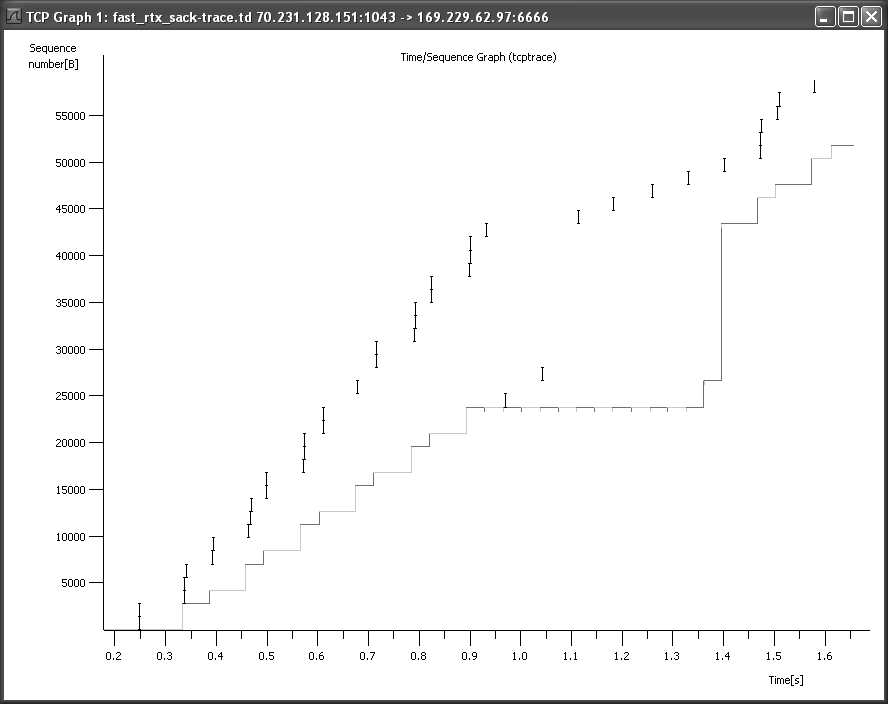
\includegraphics[width=0.7\textwidth]{imgs/14/14-9.png}
	\caption{第一个包含SACK 信息的重复ACK 触发了快速重传。后一个ACK 的到达使得发送端了解到第二个丢失的报文段,并在同一个 RTT 内重传了该报文段}
\end{figure}

图14-9与图14-6类似,但利用SACK信息,发送端在重传完报文段23601 后,不必等待一个 RTT 再重传丢失报文段28801。后面将仔细讨论这些内容,现在我们首先在连接建立
过程中验证 SACK 允许(SACK-Permitted) 选项的存在,见图14-10。

\begin{figure}[!htb]
    \centering
	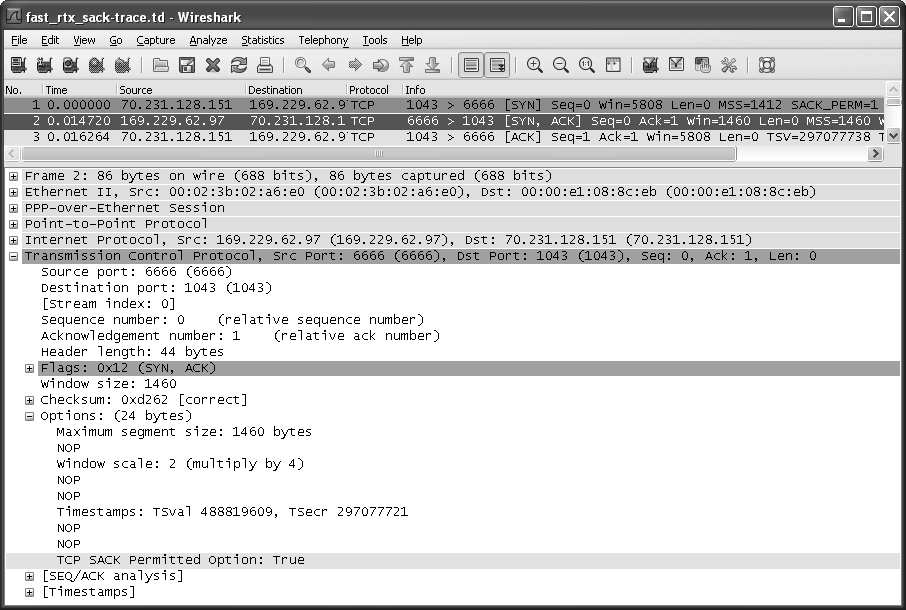
\includegraphics[width=0.9\textwidth]{imgs/14/14-10.png}
	\caption{SYN 报文段中SACK 允许选项表明可生成和发送SACK信息。现在的大部分 TCP 版本在连接建立阶段都支持 MSS,时间戳,窗口扩大以及 SACK 允许选项}
\end{figure}

与预计的一样,接收端通过SACK允许选项来使用SACK。发送端的SYN 包,即记录的第一个包,也包含了该选项。这些选项只在连接建立阶段才能看到,因此只出现在SYN置位的报文段中。

一旦连接被允许使用SACK,发生丢包即会使得接收端开始生成SACK。Wireshark 显示了第一个 SACK 选项的内容(见图14-11)。

\begin{figure}[!htb]
    \centering
	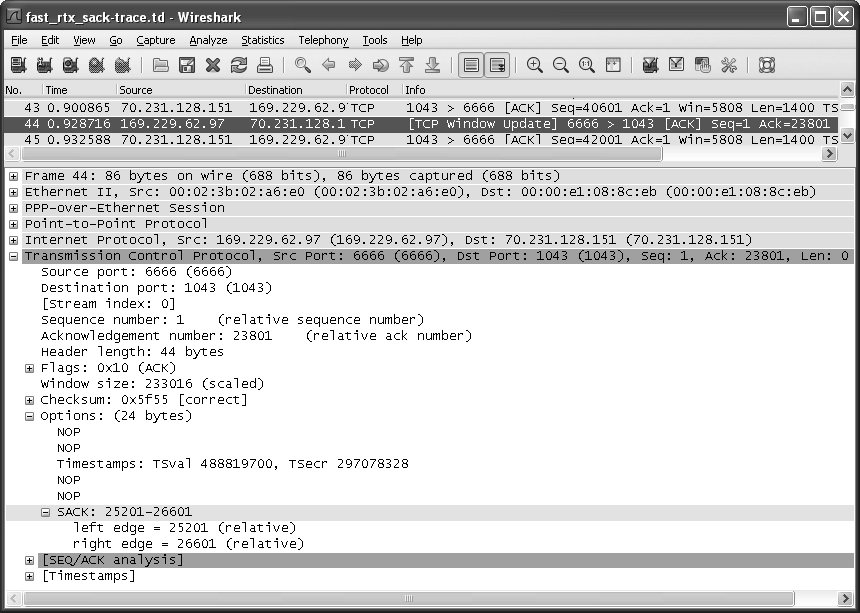
\includegraphics[width=0.7\textwidth]{imgs/14/14-11.png}
	\caption{第一个 ACK 包含SACK 信息表明失序数据的序列号范围为 25201 至 26601}
\end{figure}

图14-11 显示了首个SACK 被接收后的一系列事件。Wireshark 通过SACK 范围的左右边界来表示 SACK 信息。这里我们看到 23801的ACK 包含了一个SACK 块[25201,26601],
指明接收端的空缺。接收端敏失的序列号范围为[23801,25200],相当于一个从序列号23801开始的 1400字节的包。注意到该 SACK 为一次窗口更新,并不能算作重复ACK,之
前也提到过,因此不能触发快速重传。

0.967S时刻到达的SACK 包含两个块:[28001,29401]和[25201, 26601]。回忆一下前面提过的,为提高对 ACK 丢失的鲁棒性,前面SACK 的第一个块需要重复出现在后续
SACK 的靠后的位置。该SACK 为序列号23801的重复 ACK,表明接收端现在需要从序列号23801至26601 的两个全长报文段。发送端立即响应,启动快速重传,但由于拥塞控制机
制(见第16章),发送端只重传了一个报文段23801。随着另外的两个ACK 的到达,发送端被允许发送第二个重传报文段26601。

TCP SACK 发送端借鉴了 NewReno算法中的恢复点的思想。本例中,在重传前发送的最大序列号为 43400,低于图14-5所示的NewReno算法的例子。这里的SACK 快速重传实
现中,不需要三次重复 ACK;TCP 更早地启动了重传,但恢复的出口本质上是一致的。一且接收到序列号 43401 的 ACK,即1.3958s时刻,恢复阶段即完成。

值得注意的是,发送端采用SACK 并不能百分百地提高整体传输性能。我们来看之前讨论过的这两个例子,NewReno 发送端(非 SACK)完成131 074字节的数据传输用时3.529s,
而SACK 发送端则用了3.674s。尽管这两个值不能这样直接比较,因为两者所处的网络环境并非绝对相同(这不是仿真实验,而是在真实环境中的测试),但极为近似。在RTT较大,
丢包严重的情况下,SACK 的优势就能很好地体现出来,因为在这样的环境下,一个 RTT内能填补多个空缺显得尤为重要。

\section{伪超时与重传}
在很多情况下,即使没有出现数据丢失也可能引发重传。这种不必要的重传称为伪重传 (spurious retransmission),其主要造成原因是伪超时(spurious timeout),即过早判定超时,
其他因素如包失序、包重复,或ACK 丢失也可能导致该现象。在实际 RTT 显著增长,超过当前 RTO 时,可能出现伪超时。在下层协议性能变化较大的环境中(如无线环境),这种情
况出现得比较多,[KP87]中也提到。这里我们仅关注由伪超时导致的伪重传。失序与重复的影响在下面的章节中再讨论。

为处理伪超时问题提出了许多方法。这些方法通常包含检测(detection)算法与响应(response)算法。检测算法用于判断某个超时或基于计时器的重传是否真实,一旦认定出现
伪超时则执行响应算法,用于撤销或减轻该超时带来的影响。本章中我们只讨论报文段重传行为。典型的响应算法也涉及拥塞控制变化,会在第16章讨论。

图14-12描述了一个简化的TCP 交换过程。在报文段8发送完成后 ACK 链路上出现了延迟高峰导致了一次伪重传。在报文段5超时重传后,原始传输的报文段5~8的ACK
仍然处于在传状态。本图中为简便起见,序列号和 ACK号都基于包而非字节来表示,并且ACK 号表示已接收到的包,而非期望接收的下一个包。当这些 ACK 到达时,发送端继续重
传早已接收的其他报文段,从已确认的报文段之后开始。这导致 TCP 出现了“回退 N”(g0-back-N)的行为模式,并产生了更多的重复 ACK 返回发送端,这时就可能会触发快速重传。
针对这一问题,提出了一些方法来减轻不良影响。下面我们讨论其中比较常用的几种方法。

\subsection{重复 SACK (DSACK)扩展}
在非SACK 的TCP 中,ACK 只能向发送端告知最大的有序报文段。采用SACK 则可告知其他的(失序)报文段。基本的SACK 机制对接收端收到重复数据段时怎样运作没有规定。
这些重复数据可能是伪重传、网络中的重复或其他原因造成的。

在传输完报文段8后出现了一次延迟高峰,导致了报文段5的伪超时和重传。重传完成后,首次传输的报文段5对应的ACK 到达。报文段5的重传使得接收端收到了重复报文段,紧接着又重传了报文段6、7、8,尽管在接收端已存在这些报文段,整个连接还是执行了“回退N”行为

在SACK 接收端采用 DSACK(或称作 D-SACK),即重复 SACK[RFC2883],并结合通常的 SACK 发送端,可在第一个 SACK 块中告知接收端收到的重复报文段序列号。DSACK
的主要目的是判断何时的重传是不必要的,并了解网络中的其他事项。因此发送端至少可以推断是否发生了包失序、ACK 丢失、包重复或伪重传。

DSACK 相比于传统SACK 并不需要额外的协商过程。为使其正常工作,接收端返回的SACK 的内容会有所改变,对应的发送端的响应也会随之变化。如果一个非 DSACK 与
DSACK 的 TCP 共用一个连接,它们会交互操作,但非DSACK 不能使用DSACK 的功能。

SACK 接收端的变化在于,允许包含序列号小于(或等于)累积 ACK 号字段的SACK块。这并非SACK 的本意,但这样做能很好地配合该目的。(在 DSACK 信息高于累积 ACK
号字段的情况下,即出现重复的失序报文段时,它也能很好地工作。)DSACK 信息只包含在单个 ACK 中,该ACK 称为DSACK。与通常的SACK 信息不同,DSACK 信息不会在多个
SACK 中重复。因此,DSACK 较通常的 SACK 鲁棒性低。

[RFC2883]没有具体规定发送端对DSACK 怎样处理。[RFC3708] 给出了一种实验算法,利用DSACK来检测伪重传,但它并没有提供响应算法。它提到可采用 Eifel 响应算法,我
们在14.7.4 节中会讨论,在此之前我们先介绍一些其他的检测算法。

\subsection{Eifel 检测算法}
本章开头,我们讨论了重传二义性问题。实验性的 Eifel 检测算法TRFC3522]利用了TCP的ISOPT来检测伪重传。在发生超时重传后,Eifel 算法等待接收下一个ACK,若为针
对第一次传输(即原始传输)的确认,则判定该重传是伪重传。

利用Eifel 检测算法能比仅来用DSACK 更早检测到伪重传行为,因为它判断伪重传的ACK 是在启动丢失恢复之前生成的。相反,DSACK 只有在重复报文段到达接收端后才能发
送,并且在DSACK返回至发送端后才能有所响应。及早检测伪重传更为有利,它能使发送端有效避免前面提到的“回退N”行为。

Eifel 检测算法的机制很简单。它需要使用TCP 的TSOPT。当发送一个重传(不论是基于计时器的重传还是快速重传)后,保存其 TSV 值。当接收到相应分组的ACK 后,检查该
ACK 的TSER 部分。若 TSER值小于之前存储的TSV 值,则可判定该ACK 对应的是原始传输分组,即该重传是伪重传。这种方法针对ACK 丢失也有很好的鲁棒性。如果一个ACK
丢失,后续ACK 的TSBR 值仍比存储的重传分组的TSV小。该窗口内的任一ACK 的到达都能判断是否出现伪重传,因此单个ACK 的丢失不会造成太大问题。

Eifel 检测算法可与DSACK 结合使用,这样可以解决整个窗口的ACK 信息均丢失,但原始传输和重传分组都成功到达接收端的情况。在这种特殊情况下,重传分组的到达会生成
一个 DSACK。Eifel 算法会理所当然地认定出现了伪重传。然而,在出现了如此之多的ACK丢失的情况下,使得 TCP 相信该重传不是伪重传是有用的(例如,使其减慢发送速率—采
用拥塞控制的后果,第16章会讨论)。因此,DSACK 的到达会使得 Eifel 算法认定相应的重传不是伪重传。

\subsection{前移 RTO 恢复(F-RTO)}
前移 RTO 恢复(Forward-RTO Recovery,F-RTO)[RFC5682]是检测伪重传的标准算法。它不需要任何 TCP选项,因此只要在发送端实现该方法后,即使针对不支持 TSOPT 的接收
端也能有效地工作。该算法只检测由重传计时器超时引发的伪重传;对之前提到的其他原因引起的伪重传则无法判断。

在一次基于计时器的重传之后,F-RTO 会对TCP的常用行为做出一定修改。由于这类重传针对的是没有收到 ACK 信息的最小序列号,通常情况下,TCP 会继续按序发送相邻的
分组,这就是前面描述的“回退N”行为。

F-RTO 会修改 TCP 的行 ,在超时重传后收到第一个 ACK 时,TCP 会发送新(非重传)数据,之后再响应后一个到达的ACK。如果其中有一个为重复ACK,则认为此次重传没问
题。如果这两个都不是重复ACK,则表示该重传是伪重传。这种方法比较直观。如果新数据的传输得到了相应的ACK,就使得接收端窗口前移。如果新数据的发送导致了重复ACK,
那么接收端至少有一个或更多的空缺。这两种情况下,接收新数据都不会影响整体数据的传输性能(假设接收端有足够的存储空间)。

\subsection{Eifel 响应算法}
一旦判断出现伪重传,则会引发一套标准操作,即 Eifel 响应算法[RFC4015]。由于响应算法逻辑上与 Eifel 检测算法分离,所以它可与我们前面讨论的任一种检测方法结合使
用。原则上超时重传和快速重传都可使用Eifel 响应算法,但目前只针对超时重传做了相关规定。

尽管 Eifel 响应算法可结合其他检测算法使用,但根据是否能尽早(如 Eifel 检测算法或F-RTO)或较迟(如DSACK)检测出伪超时的不同而有所区别。前者称为伪超时,通过检查
ACK 或原始传输来实现。后者称为迟伪超时(late spurious timeout),基于由(伪)超时而引发的重传所返回的ACK 来判定。

响应算法只针对第一种重传事件。若在恢复阶段完成之前再次发生超时,则不会执行响应算法。在重传计时器超时后,它会查看 srt 和 rttvar 的值,并按如下方式记录新的变量
\verb|srtt_prev| 和 \verb|rttvar_prev|:

\begin{verbatim}
    srtt_prev = srtt + 2(G)
rttvar prev = rttvar
\end{verbatim}

在任何一次计时器超时后,都会指定这两个变量,但只有在判定出现伪超时才会使用它们,用于设定新的 RTO。在上式中,G代表TCP 时钟粒度。\verb|srtt_prev| 设为 sttt加上两倍的时钟
粒度是由于:srt的值过小,可能会出现伪超时。如果 srtt稍大,就可能不会发生超时。sttt加上2G 得到 \verb|srtt_prev|,之后都使用 \verb|srtt_prev| 来设置 RTO。

完成 \verb|srtt_prey| 和 \verb|rttvar_prev| 的存储后,就要触发某种检测算法。运行检测算法后可得到一个特殊的值,称为伪恢复(SpuriousRecovery)。如果检测到一次伪超时,则将伪恢复置为
\verb|SPUR_TO|。如果检测到迟伪超时,则将其置为 \verb|LATB_SPUR_TO|。否则,该次超时为正常超时,TCP继续执行正常的响应行为。

若伪恢复为 \verb|SPUR_TO.TCP|可在恢复阶段完成之前进行操作。通过将下一个要发送报文段(称为 SND.NXT)的序列号修改为最新的未发送过的报文段(称为 SND.MAX)。这样
就可在首次重传后避免不必要的“回退N”行为。如果检测到一次迟伪超时,此时已生成对首次重传的ACK,则SND.NXT 不改变。在以上两种情况中,都要重新设置拥塞控制状态
(见第16章)。并且一旦接收到重传计时器超时后发送的报文段的ACK,就要按如下方式更新 srtt、rttvar 和 RTO 的值:

这里,m是一个 RTT样本值,它是基于超时后首个发送数据收到的ACK 而计算得到的。进行这些变量更新的目的在于,实际的RTT值可能发生了很大变化,RTT 的当前估计值已
经不适合用于设置 RTO。若路径上的实际 RTT 突然增大(例如由于无线切换至一个新的基站),当前的 srtt和rttvar 就显得过小,应重新设置。而另一方面,RTT 的增大可能只是暂时
的,这时重设 srtt 和 rttvar 的值就不那么明智了,因为它们原先的值可能更为精确。

在新RTT 样本值较大的情况下,上述等式尽力获得上述两种情况的平衡。这样做可以有效地抛弃之前的 RTT 历史值(和 RTT 的历史变化情况)。只有在响应算法中 srtt和 rttvar
的值才会增大。若RTT 不会增大,则维持估计值不变,这本质上是忽略超时情况的发生。两种情况中,RTO还是按正常方式进行更新,并针对此次超时设置新的重传计时器值。

\section{包失序与包重复}
前面讨论的都是 TCP 如何处理包丢失的问题。这是普遍讨论的问题,而且针对包丢失的鲁棒性问题已经做了很多工作。在最后一个章节中可以看到,其他的包传输异常现象,如
重复和失序问题也会影响 TCP操作。在这两种情况中,我们希望 TCP 能区分是出现了失序或重复还是丢失。我们接下来会看到,正确区分这些情况并非易事。


\subsection{}
在IP网络中出现包失序的原因在于IP 层不能保证包传输是有序进行的。这一方面是有利的(至少对IP 层来说),因为IP 可以选择另一条传输链路(例如传输速度更快的路径),而
不用担心新发送的分组会先于旧数据到达,这就导致数据的接收顺序与发送顺序不一致。还有其他的原因也会导致包失序。例如,在硬件方面一些高性能路由器会采用多个并行数据链
路[BPS99],不同的处理延时也会导致包的离开顺序与到达顺序不匹配。

失序问题可能存在于 TCP 连接的正向或反向链路中(也可能两者同时存在)。数据段的失序与 ACK 包的失序对 TCP 的影响有一定差别。回忆一下,由于非对称路由,经常会出现
ACK 经不同于数据包的链路(和不同路由器)传输。

当传输出现失序时,TCP 可能会在某些方面受影响。如果失序发生在反向(ACK)链路,就会使得 TCP 发送端窗口快速前移,接着又可能收到一些显然重复而应被丢弃的ACK。由
于TCP 的拥塞控制行为(见第16章),这种情况会导致发送端出现不必要的流量突发(即瞬时的高速发送)行为,影响可用网络带宽。

如果失序发生在正向链路,TCP 可能无法正确识别失序和丢包。数据的丢失和失序都会导致接收端收到无序的包,造成数据之间的空缺。当失序程度不是很大(如两个相邻的包交
换顺序),这种情况可以迅速得到处理。反之,当出现严重失序时,TCP 会误认为数据已经丢失。这就会导致伪重传,主要来自快速重传算法。

回忆一下之前的讨论,快速重传是根据收到重复ACK 来推断出现丢包并启动重传,而不必等待重传计时器超时。由于 TCP 接收端会对接收到的失序数据立即返回ACK,以此来
帮助触发快速重传,因此网络中任何一个失序的数据包都会生成重复 ACK。由于网络中少量失序情况是常见的,假设一旦收到重复 ACK,发送端即启动快速重传,那么就会导致大量不
必要的重传发生。为解决这一问题,快速重传仅在达到重复阈值(dupthresh) 后才会被触发。

图14-13描述了上述情况。图中左半部分表示在轻微失序的情况下 TCP 的操作,这里的dupthresh 设为3。单个重复ACK 不会影响TCP的行。右半部分表示出现严重失序时的情
况。由于出现了3次失序,对应生成了3次重复 ACK,因此触发了快速重传,使得接收端收到了一个重复报文段。


轻徽失序(左)中,可忽略少量的重复ACK。当失序状况较为严重(右)时,这里4个包中有三个出现失序,就会触发伪快速重传

区分丢包与失序不是一个很重要的问题。要解决它需要判断发送端是否已经等待了足够长的时间来填补接收端的空缺。幸运的是,互联网中严重的失序并不常见[J03],因此将
dupthresh 设为相对较小值(如峡省值为3)就能处理绝大部分情况。即便如此,还是有很多研究致力于调整 TCP 行为来应对严重失序[LLY07]。有些方法可动态调整 dupthresh,如
Linux 的TCP实现。

\subsection{重复}
尽管出现得比较少,但IP协议也可能出现将单个包传输多次的情况。例如,当链路层
网络协议执行一次重传,并生成同一个包的两个副本。当重复生成时,TCP 可能出现混淆。考虑图14-14 中的情况,包3重复生成三个副本。

从图中可看到,包3的多次重复会使得接收端生成一系列的重复ACK,这足以触发伪快速重传,使得非 SACK
发送端误认为包5与包6更早到达。利用SACK(特别是DSACK),就可以简单地忽略这个问题。采用DSACK,每个A3的重复 ACK 都包含报文段3已成功接收的信息,并且没
有包含失序数据信息,意味着到达的包(或ACK)一定是重复数据。TCP 通常都可防止此类伪重传。

\section{目的度量}
从前面的讨论中我们看到,TCP 能不断“学习”发送端与接收端之间的链路特征。学习的结果显示为发送端记录一些状态变量,如srtt和 rttvar。一些 TCP 实现也记录一段时间内已出现的失序包的估计值。
一般来说,一旦该连接关闭,这些学习结果也会丢失,即与同一个接收端建立一个新的TCP连接后,它必须从头开始获得状态变量值。

较新的TCP 实现维护了这些度量值,即使在连接断开后,也能保存之前存在的路由或转发表项,或其他的一些系统数据结构。当创立一个新的连接时,首先查看数据结构中是否
存在与该目的端的先前通信信息。如果存在,则选择较近的信息,据此为 srtt、rttvar 以及其他变量设初值。在TCP 连接关闭前,可更新统计数据,通过替换现存数据或其他方式的
更新来实现。在Linux 2.6中,变量值更新为现存值中的最大值和最近测量的数据。可通过iproute2[IPR2]的相关工具来查看这些变量值:

\begin{verbatim}
    Linux& ip route show cache 132.239.50.184
132.239.50.184 from 10.0.0.9 tos 0x10 via 10.0.0.1 dev
mtu 1500 rtt 29ms rttvar 29ms cwnd 2 advmss 1460 hoplimit 64
\end{verbatim}


该命令利用特的DSCP 值(16,表示CS2,但值为 Ox10代表采用较旧日的“Tos”)显示了之前连接存储的信息,本地系统和 132.239.50.184之间采用IPv4,下一跳为10.0.0.1
网络设备为 ehto。我们可以看到包大小信息(由 PMTUD 得到路径MTU,由远端告知MSS)、最大跳步数(针对IPv6,这里没有用到)、stt 和 rttvar 的值,以及第16章中会讨论
的拥塞控制信息如 cwnd。

\section{重新组包}

当TCP超时重传,它并不需要完全重传相同的报文段。TCP允许执行重新组包(repacketization),发送一个更大的报文段来提高性能。(通常该更大的报文段不能超过接收
端通告的 MSS,也不能大于路径 MTU。)允许这样做的原因在于,TCP是通过字节号来识别发送和接收的数据,而非报文段(或包)号。

TCP能重传一个与原报文段不同大小的报文段,这从一定意义上解决了重传二义性问题。STODER[T2205] 就是基于该思想,采用重新组包的方法来检测伪超时。

我们可以很容易地观察到重新组包的过程。我们采用 sock 程序作为服务器,并用 Telnet连接它。首次我们输人一行信息 “hello there”。这就生成了一个13字节的数据段,包括回
车换行在内。接着断开网络连接,输人 “line number 2”(14字节,包括换行)。然后在等待约45秒后,输入“and 3",之后关闭连接:

在分析结果中,省略了初始SYN交换过程。前两个报文段包含数据字符串“hellothere ”及其确认信息。紧接着的包并非有序:它从序列号29开始,包含字符串 “and 3"(7
个字节)。它返回的ACK包含ACK 号14,但SACK 块的相对序列号为(29,36}。中间的数据已丢失。TCP 采用一个更大的包来重传,包含序列号14 ~36。因此,我们可以看到序
列号14数据的重传导致了一次重新组包,形成了 22 字节的较大包来传输。有趣的是,包中重复包含了 SACK 块中的数据,同时也将 FIN 位字段置位,表明这是连接关闭前最后传输的
数据。

\section{与TCP 重传相关的攻击}
有一类DoS 攻击称为低速率 DoS 攻击[KK03]。在这类攻击中,攻击者向网关或主机发送大量数据,使得受害系统持续处于重传超时的状态。由于攻击者可预知受害 TCP 何时
启动重传,并在每次重传时生成并发送大量数据。因此,受害 TCP 总能感知到拥塞的存在,根据 Kam 算法不断减小发送速率并退避发送,导致无法正常使用网络带宽。针对此类攻击
的预防方法是随机选择 RTO,使得攻击者无法预知确切的重传时间。

与 Dos相关但不同的一种攻击为减慢受害 TCP的发送,使得 RTT估计值过大。这样受害者在丢包后不会立即重传。相反的攻击也是有可能的:攻击者在数据发送完成但还未到达
接收端时伪造 ACK。这样攻击者就能使受害 TCP 认为连接的 RTT 远小于实际值,导致过分发送,造成大量的无效传输。


\section{总结}
本章详细讨论了 TCP 超时和重传策略。第一个例子描述了当TCP需要发送一个数据包时,简单地暂时断开网络,导致重传计时器超时触发了一次超时重传。每个后续重传与前一
次传输都间隔两倍时长,形成二进制指数退避,即 Kar 算法的第二部分。

TCP 测量 RTT 并用这些测量值记录平滑的RTT 与均值偏差估计值,用这两个估计值计算新的重传超时值。在不采用时间戳选项的情况下,TCP 在每个数据窗口只能测量一个
RTT。Kam 算法通过不测量重传报文段的 RTT样本值来避免重传二义性问题。现在的大部分TCP 版本都使用时间戳选项,使得每个报文段都能单独测量。时间戳选项即使在包失序
或包重复的情况下也能很好地工作。

我们还讨论了快速重传算法,它在计时器没有超时的情况下就能被触发。该算法可有效地(并最常用)填补由丢包引起的空缺。结合选择确认可更好地提高算法性能。选择确认在
ACK 中携带其他的信息,允许发送端在每个 RTT 内修补多个空觖,在某些环境下可有效提高传输性能。

如果 RTT 测量值小于连接的实际值,就可能发生伪重传。在这种情况下,若TCP 的等待时间稍长,(不必要的)重传就可能不会发生。针对伪超时问题提出了很多算法。DSACK
需要等到接收到重复报文段的ACK。Eifel 检测方法依据 TCP 时间戳,但它的响应速度能比DSACK 更快,这是因为它是根据超时前所发送报文段返回的ACK 来检测伪超时的。F-RTO
与 Eifel 算法类似,但不需要时间戳。它使得发送端在判断出现伪超时后发送新数据。以上这些检测算法都需要结合使用响应算法,我们讨论到的响应算法主要是 Eifel 响应算法。它
在延迟大幅增长的情况下(否则对超时不做任何响应),会重新设置 RTT 和 RTT变化估计值。

我们也讨论了 TCP 怎样存储连接状态,怎样重新组包,以及相关攻击,包括使得 TCP过分被动或过分积极。在第16章讨论 TCP拥塞控制时,我们会看到更多的此类攻击及其造
成的影响。
\chapter{TCP数据流和与窗口管理}
\minitoc

\section{引言}
第13章介绍了 TCP 连接的建立和终止,第14章则讨论了TCP 怎样利用丢失数据的重传来保证传输可靠性。下面我们探讨TCP的动态数据传输,首先关注交互式连接,接着介
绍流量控制以及窗口管理规程。批量数据传输中的拥塞控制策略(参见第16章)也包含了相应的窗口管理机制。

“交互式”TCP连接是指,该连接需要在客户端和服务器之间传输用户输入信息,如按键操作、短消息、操作杆或鼠标的动作等。如果采用较小的报文段来承载这些用户信息,那
么传输协议需要耗费很高的代价,因为每个交换分组中包含的有效负载字节较少。反之,报文段较大则会引入更大的延时,对延迟敏感类应用(如在线游戏、协同工具等)造成负面影
响。因此我们需要权衡相关因素,找到折中方法。

在讨论交互式通信的相关问题后,会介绍 TCP流量控制机制。它通过动态调节窗口大小来控制发送端的操作,确保接收端不会溢出。这个方法主要用于批量数据传输(即非交互
式通信),但对交互式应用也同样有效。在第16章我们会看到,流量控制的思想也可以扩展应用于其他问题,不仅可以保护接收端免于溢出,还可处理中间传输网络的拥塞问题。
\section{交互式通信}

在一定时间内,互联网的不同部分传输的网络流量(通常以字节或包来计算)也存在相当大的差异。例如,局域网与广域网以及不同网站之间的流量都会有所不同。TCP 流量研究
表明,通常90\%或者更多的 TCP报文段都包含大批量数据(如Web、文件共享、电子邮件、备份),其余部分则包含交互式数据(如远程登录、网络游戏)。批量数据段通常较大(1500
字节或更大),而交互式数据段则会比较小(几十字节的用户数据)。

对于使用相同协议以及封包格式的数据,TCP都会处理,但执行的算法有所不同。在本节中我们会讨论 TCP 如何传输交互式数据,以 ssh(安全外壳)应用为例。安全外壳协议
[RFC4251]是具备较强安全性(基于密码学的加密和认证)的远程登录协议。它已经基本取代了早期的 UNIX tlogin 和 Telnet,因为这些远程登录服务都存在安全隐患。

通过对ssh的探讨,我们会了解延时确认是怎样工作的,以及 Nagle 算法怎样实现减少广域网中较小包的数目。同样的算法也可以用于其他远程登录应用,如 Telnet、rlogin 和微
软终端服务。

对一个 ssh 连接,观察当我们输人一个交互命令后的数据流。客户端获取用户输入信息,然后将其传给服务器端。服务器对命令进行解释并生成响应返回给客户端。客户端对其
传输数据加密,意味着用户输入的信息在通过连接传送前已经进行了加密(参见第18章)。即使传输数据被被获,窃听者也很难获得用户输入信息的明文。客户端支持多种加密算法
和认证方法。它也支持一些新的特性,如隧道技术实现对其他协议的封装(参见第3章及[RFC4254])。

许多 TCP/IP 的初学者会惊奇地发现,每个交互按键通常都会生成一个单独的数据包。也就是说,每个按键是独立传输的(每次一个字符而非每次一行)。另外,ssh 会在远程系统
(服务器端)调用一个 shell(命令解释器),对客户端的输人字符做出回显。因此,每个输人的字符会生成4个 TCP数据段:客户端的交互击键输人、服务器端对击键的确认、服务器端
生成的回显、客户端对该回显的确认(参见图15-1a)。

通常,第2和第3段可以合并,如图15-1b所示,可将对击键的确认与回显一并传送。下一节会介绍这种方法(称力捎带延时璃认)。

a)对一次交互击键的远程回显,一种可行的方法是将对击键的确认与回显包各自独立发送。b)典型 TCP 则将两者结合传输

我们以 ssh 为例的原因在于,对从客户端到服务器键人的每个字符都会生成一个独立的包。然而,若用户的输入速度较快,每个包可能包含多个字符。图15-2显示了在ssh 连接至
Linux 服务器中输入 date 命令,利用 Wireshark 获得的数据流。

\begin{figure}[!htb]
    \centering
	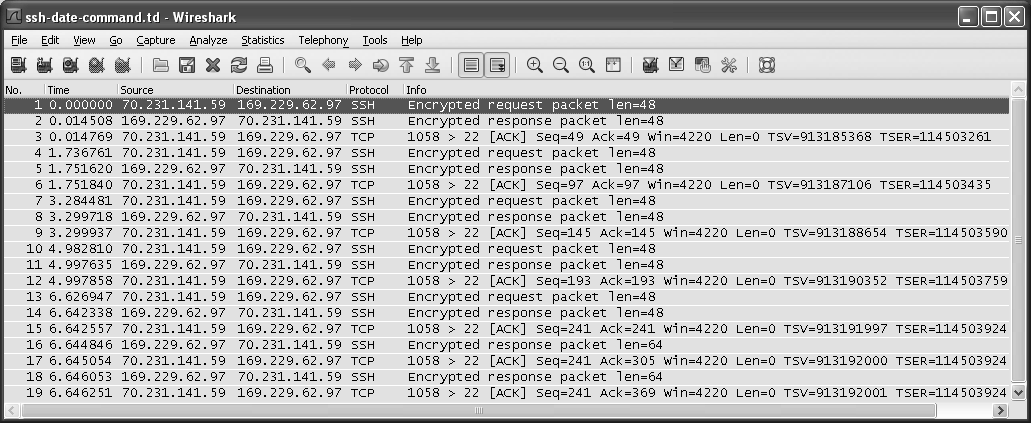
\includegraphics[width=0.7\textwidth]{imgs/15/15-2.png}
	\caption{变得更为密集。Linux 避免 RTO 设置过小就是防止这种情况的发生。标准方法在样本 78 和191 出现潜在问题}
\end{figure}

如图15-2所示,包1包含了客户端到服务器端的命令字符d。包2为对字符d的确认和回显(如图15-] 中将两段结合传送)。包3为对国显字符d的确认。同理,包4~6对应字
符日,包7-◎对应字符1,包10~12对应字符e。包13~15 则对应回车键。在包3+6~7、9~10和12~13 之间的时间差为人工输入每个字符的延迟,这里特意设置得较长
(约1.5秒)。

注意到包16~19与前面的包稍有差异,包长度从48字节变为64字节。包16包含了服务器端对 date 命令的输出。这64 字节的数据是对下面28个明文(未加密)字符的加密
结果:
\begin{verbatim}
    Wed Dec 28 22:47:16 PST 2005
\end{verbatim}
加上最后的回车和换行符。下一个从服务器端发送至客户端的包(包18)包含了服务器主机对客户的命令提示符:Linux\%。包19为对该数据的确认。

图15-3描述与图15-2相同的传输情况,只是细化了 TCP 层的信息,可以更清晰地看到TCP 怎样进行确认以及 ssh 使用的包大小。包1(包含字符d)的相对序列号从0开始。包2
是对图中包1的确认,ACK 号设为48,为上次成功接收字节的序列号加1。包2也包含了服务器至客户端的对d字符的回显,字节序列号为0。包3为客户端对该回显的确认,ACK
号设为 48。可以看到,该连接包含了两个序列号流个是从客户端至服务器,另一个为相反方向。在介绍窗口通告时将会详细讨论这一问题。

\begin{figure}[!htb]
    \centering
	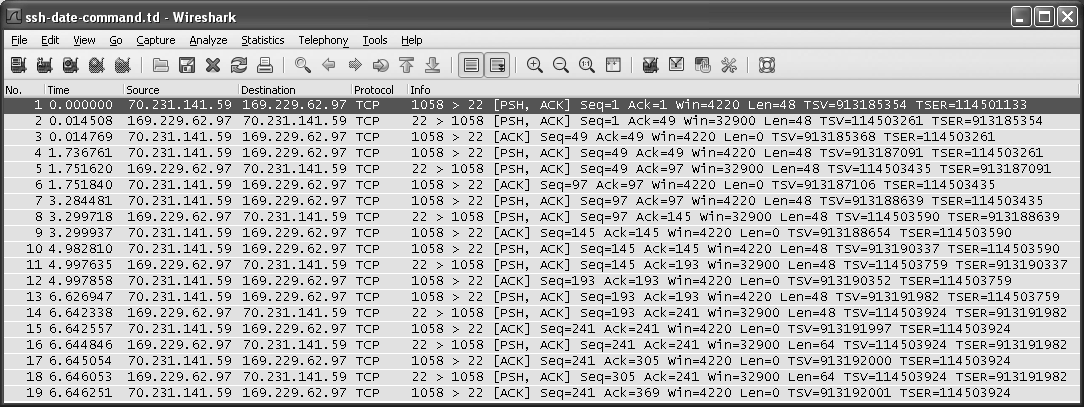
\includegraphics[width=0.7\textwidth]{imgs/15/15-3.png}
	\caption{与图 15-2相同,只是这里禁用了 ssh 的协议解码,因此可以看到 TCP 序列号信息。注意到除了最后两个包外,其他包都为48字节,该长度与 ssh 使用的加密算法有关(参见第18章)}
\end{figure}

另外我们也发现,每个带数据(长度不为0)的包都将PSH置位。之前提到过,该标志位通常表示发送端缓存为空。也就是说,当PSH 置位的数据包发送完成后,发送端没有其
他数据包需要传输。

\section{延时确认}
在许多情况下,TCP 并不对每个到来的数据包都返回 ACK,利用TCP 的累积ACK 字段(参见第12 章)就能实现该功能。累积确认可以允许 TCP 延迟一段时间发送ACK,以便
将 ACK 和相同方向上需要传的数据结合发送。这种捎带传输的方法经常用于批量数据传输。显然,TCP 不能任意时长地延迟ACK;否则对方会误认为数据丢失而出现不必要的重传。

\begin{tcolorbox}
    主机需求 RFC [RFC1122]指出,TCP 实现 ACK 延迟的时延应小于 500ms。实践中时延最大取 200ms。
\end{tcolorbox}

采用延时 ACK的方法会减少ACK 传输数目,可以一定程度地减轻网络负载。对于批量数据传输通常为2:1的比例。基于不同的主机操作系统,延迟发送ACK 的最大时延可以
动态配置。Linux 使用了一种动态调节算法,可以在每个报文段返回一个ACK(称次“快速确认”模式)与传统延时ACK 模式间相互切换。Mac OS X 中,可以改变系统变量 
\verb|net.inet.top.delayed_ack| 值来设置延时 ACK。可选值如下:禁用延时(设为0),始终延时(设为1),每隔一个包回复一个 ACK(设为2),自动检测确认时间(设次3)。默认值为3。最新的
Windows 版本中,注册表项
\begin{verbatim}
    HKLM\SYSTEM\CurrentControlSet\Services\Tcpip\Parameters\Interfaces\IG
\end{verbatim}
中,每个接口的全局唯一标识(GUID)都不同(IG 表示被引用的特定网络接口的GUID)。TepAckFrequency 值(需要被添加)可以设为0~255,默认为2。它代表延时 ACK 计时器
超时前在传的ACK 数目。将其设为1表明对每个收到的报文段都生成相应的ACK。ACK 计时器值可以通过 TopDelAckTicks注册表项控制。该值可设为2~6,默认为2。它以百毫秒
为单位,表明在发送延时ACK 前要等待百毫秒数。

之前提到过,通常 TCP 在某些情况下使用延时 ACK 的方法,但时延不会很长。在第16章中大量采用了延时 ACK 的方法,我们将会看到 TCP怎样在处理批量数据的大数据包传输
中实现拥塞控制。在小数据包传输中,如交互式应用,需要采用另外的算法。将该算法与延时 ACK 结合使用,如果处理不好,反而会导致性能降低。下面我们详细讨论该算法。

\section{Nagle 算法}
从前面的小节中可以知道,在ssh 连接中,通常单次击键就会引发数据流的传输。如果使用 IPv4,一次按键会生成约88字节大小的TCP/IPv4包(使用加密和认证):20字节的
『头部,20字节的TCP 头部(假设没有选项),数据部分为48字节。这些小包(称为微型报(tinygram))会造成相当高的网络传输代价。也就是说,与包的其他部分相比,有效的应
用数据所占比例甚微。该问题对于局域网不会有很大影响,因为大部分局域网不存在拥塞,而且这些包无须传输很远。然而对于广域网来说则会加重拥塞,严重影响网络性能。John
Nagle 在[RFC0896]中提出了一种简单有效的解决方法,现在称其为 Nagle 算法。下面首先介绍该算法是怎样运行的,接着我们会讨论结合延时 ACK 方法使用时可能出现的一些缺陷
和问题。

Nagle算法要求,当一个 TCP 连接中有在传数据(即那些已发送但还未经确认的数据),小的报文段(长度小于 SMSS)就不能被发送,直到所有的在传数据都收到ACK。并且,在
收到ACK 后,TCP 需要收集这些小数据,将其整合到一个报文段中发送。这种方法迫使TCP 遵循停等(stop-and-wait)规程—只有等接收到所有在传数据的ACK 后才能继续发
送。该算法的精妙之处在于它实现了自时钟(self-clocking)控制:ACK 返回越快,数据传输也越快。在相对高延迟的广域网中,更需要减少微型报的数目,该算法使得单位时间内发
送的报文段数目更少。也就是说,RTT 控制着发包速率。

从图15-3中可以看到,单个字节的发送、确认以及回显的RTT较小(15ms 以下)。为更快地生成数据,我们需要每秘钟输入60个字符以上。这意味着,当两台主机之间以很小
的 RTT传输数据时,例如在同一个局域网中,我们将很难看到该算法的显著效果。

为了显示 Nagle算法的效果,我们比较分析某个 TCP 应用使用和禁用该算法的行为。我们对一个 ssh 版本的客户端做了一定的修改。利用一个 RTT相对较大(约190ms)的连接,
就可以看出区别。首先观察禁用 Nagle 算法(ssh 默认)的情况,如图15-4所示。
\begin{figure}[!htb]
    \centering
	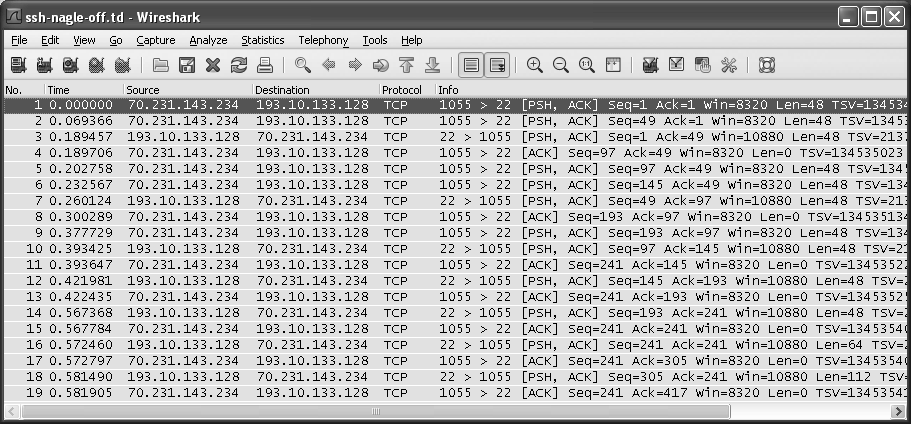
\includegraphics[width=0.7\textwidth]{imgs/15/15-4.png}
	\caption{ssh分析文件显示该TCP 连接RTT约为190ms。Nagle 算法被禁用。数据和ACK结合传输,19 个包传输持续了 0.58s。许多包相对较小(48字节的用户数据)。
    纯ACK(不包含数据的报文段)表明服务器端的输出命令已被客户端接收处理}
\end{figure}

图15-4中显示的传输是在初始的认证完成以后、登录会话开始时记录的。这时输入date 命令,我们看到共捕获到了19个包,整个传输过程持续了 0.58S。共有5个 ssh 请求包,
7个ssh 应答包,以及7个 TCP 层的纯 ACK 包(不包含数据)。下面我们将在使用Nagle算法的情况下重复探测这一过程(即在相似的网络环境下),可以得到图15-5。

RTT为190ms并启用 Nagle算法的 TCP连接的ssh传输情况。请求和响应传输规律,紧密一致。整个传输过程持续了 0.80s,共有11个包

可以看到图 15-5中的包数目要少于图15-4(少了8个)。另外一个明显的差异是,请求和响应包随时间分布呈一定的规律性。回想一下 Nagle 算法的原理,它迫使 TCP 遵循停等行
为模式,因此TCP 发送端只有在接收到全部 ACK 后才能继续发送。观察每组请求/ 响应的传输时刻—0.0、0.19、0.38以及0.57,我们可以发现它们遵循一定的模式:每两个间隔为
190ms,恰为连接的RTT。每发送一组请求和响应包需要等待一个 RTT,这就加长了整个传输过程(需要0.80s而非前面的0.58s)。Nagle 算法做出了一种折中:传输的包数目更少而长
度更大,但同时传输时延也更长。从图15-6中可以更清晰地看出差别。

图15-6显示了Nagle 算法的停等行为。左侧显示双向传输,而右侧使用 Nagle 算法,使得在任一给定时刻,只有一个方向保持传输状态。
% \begin{figure}[!htb]
%     \centering
% 	\includegraphics[width=0.7\textwidth]{imgs/15/15-6.png}
% 	\caption{比较相似环境下使用 Nagle算法与否的TCP连接情况。在启用 Nagle 算法的情况下,在任一时刻最多只有一个包在传。这样可以减少小包数目,但同时也增大了传输时延}
% \end{figure}

\subsection{延时 ACK 与 Nagle 算法结合}
若将延时ACK与Nagle 算法直接结合使用,得到的效果可能不尽如人意。考虑如下情形,客户端使用延时 ACK 方法发送一个对服务器的请求,而服务器
端的响应数据并不适合在同一个包中传输(参见图 15-7)。

从图中可以看到,在接收到来自服务器端的两个包以后,客户端并不立即发送 ACK,而是处于等待状态,希望有数据一同捎带发送。通常情况下,TCP
在接收到两个全长的数据包后就应返回一个ACK,但这里并非如此。在服务器端,由于使用了 Nagle 算法,直到收到ACK 前都不能发送新数据,因为任一
时刻只允许至多一个包在传。因此延时
ACK 与Nagle 算法的结合导致了某种程度的死锁(两端互相等待对方做出行动)[MMSV99][MMO1]。幸运的是,这种死锁并不是永久的,在延时 ACK 计时器超时后死锁会解除。客户
端即使仍然没有要发送的数据也无需再等待,而可以只发送ACK 给服务器。然而,在死锁期间整个传输连接处于空闲状态,使性能变差。在某些情况下,如这里的 ssh 传输,可以禁
用 Nagle 算法。

\subsection{禁用 Nagle 算法}
从前面的例子可以看到,在有些情况下并不适用Nagle 算法。典型的包括那些要求时延尽量小的应用,如远程控制中鼠标或按键操作需要及时送达以得到快捷的反馈。另一个例子
是多人网络游戏,人物的动作需要及时地传送以确保不影响游戏进程(也不致影响其他玩家的动作)。

禁用 Nagle 算法有多种方式,主机需求 RFC[RFC1122]列出了相关方法。若某个应用使用Berkeley 套接字 API,可以设置 \verb|TCP_NODBLAY| 选项。另外,也可以在整个系统中禁用
该算法。在 Windows 系统中,使用如下的注册表项:
\begin{verbatim}
    HKLM\ SOFTWARE \Microsoft \MSMQ \Parameters\ TCPNoDelay
\end{verbatim}
这个双字节类型的值必须由用户添加,应将其设为1。为使更改生效,消息队列也需要重新设置。

\section{流量控制与窗口管理}
回顾一下第12章中提到过,可以采用可变滑动窗口来实现流量控制。如图15-8所示,TCP 客户端和服务器交互作用,互相提供数据流的相关信息,包括报文段序列号、ACK号
和窗口大小(即接收端的可用空间)。

每个 TCP 连接都是双向的。数据传输方向的另一端会返回ACK 及其窗口通告信息。反向亦然

图15-8 中两个大的箭头表示数据流方向(TCP报文段的传输方向)。每个 TCP 都是双向连接,这里用两个箭头表示,一个是客户端至服务器方向(C一S),另一个为服务器至客户
端方向(S-C)。每个报文段包含 ACK 和窗口信息,可能还有用户数据。根据数据流传输方向的不同,将 TCP 头部中的字段标记上阴影。例如,在C一S方向的数据流为下方箭头
的报文段,但是对该数据的 ACK 和窗口信息却在上方简头指示的报文段中。每个TCP报文段(除了连接建立之初的包交换)都包含一个有效的序列号字段、一个 ACK 号或确认字段,
以及一个窗口大小字段(包含窗口通告信息)。

在前面的ssh 示例中,我们看到的窗口通告都是固定的,有8320字节、4220字节,还有32900字节。这些数值表示发送该窗口信息的通信方为即将到来的新数据预留的存储空
间。当TCP 应用程序空闲时,就会排队处理这些数据,致使窗口大小字段保持不变。当系统处理速度较慢,或者程序忙于执行其他操作,到来的数据返回ACK 后,就需要排队等待
被读取或“消耗”。若这种排队状况持续,新数据的可用存储空间就会减小,窗口大小值也随之减小。最终,若应用程序一直不处理这些数据,TCP必须采取策略使得发送端完全
停止新数据的发送,因为可能没有空间来存储新数据。此时就可以将窗口通告设为0(没有空间)。

每个 TCP 头部的窗口大小字段表明接收端可用缓存空间的大小,以字节为单位。该字段长度为16位,但窗口缩放选项可用大于65 535的值(参见第13章)。报文段发送方在相反
方向上可接受的最大序列号值为 TCP 头部中 ACK 号和窗口大小字段之和(保持单位一致)。

\subsection{滑动窗口}
TCP连接的每一端都可收发数据。连接的收发数据量是通过一组窗口结构(windowstructure)来维护的。每个 TCP活动连接的两端都维护一个发送窗口结构(send window
structure)和接收窗口结构(receive window structure)。这些结构与第12 章中描述的概念窗口结构类似,这里我们将详细讨论。图15-9显示了一个假设的TCP 发送窗口结构。

TCP 发送端滑动窗口结构记录了已确认、在传以及还未传的数据的序列号。提供窗口的大小是由接收端返回的 ACK 中的窗口大小字段控制的

TCP 以字节(而非包)为单位维护其窗口结构。在图15-9中,我们已标号为2~11字节。由接收端通告的窗口称为提供窗口(offered Window),包含4~9字节。接收端已成功
确认包括第3字节在内的之前的数据,并通告了一个6字节大小的窗口。回顾第12章,窗口大小字段相对 ACK 号有一个字节的偏移量。发送端计算其可用窗口,即它可以立即发送
的教据量。可用窗口计算值力提供窗口大小破去在传(已发送但本得到确认)的数据值。变量SND.UNA 和SND.WND 分别记录窗口左边界和提供窗口值。SND.NXT 则记录下次发送
的数据序列号,因此可用窗口值等于(SND.UNA + SND.WND -SND.NXT)。

随着时间的推移,当接收端确认数据,滑动窗口也随之右移。窗口两端的相对运动使得窗口增大或减小。可用三个术语来描述窗口左右边界的运动:
\begin{enumerate}
    \item 关闭(close),即窗口左边界右移。当已发送数据得到 ACK 确认时,窗口会减小。
    \item 打开(open),即窗口右边界右移,使得可发送数据量增大。当已确认数据得到处理,接收端可用缓存变大,窗口也随之变大。
    \item .收缩(shrink),即窗口右边界左移。主机需求 RFC[RFC1122]并不支持这一做法,但TCP必须能处理这一问题。15.5.3 节的糊涂窗口综合征中举了一个例子,一端试图将右边界左移使窗口收缩,但没有成功。
\end{enumerate}

每个TCP报文段都包含ACK 号和窗口通告信息,TCP发送端可以据此调节窗口结构。窗口左边界不能左移,因为它控制的是已确认的ACK 号,具有累积性,不能返回。当
得到的ACK 号增大而窗口大小保持不变时(通常如此),我们就说窗口向前“滑动”。若随着ACK 号增大窗口却减小,则左右边界距离减小。当左右边界相等时,称之为零窗口。此
时发送端不能再发送新数据。这种情况下,TCP 发送端开始探测(probe)对方窗口(参见15.5.2节),伺机增大提供窗口。

接收端也维护一个窗口结构,但比发送端窗口简单。该窗口结构记录了已接收并确认的数据,以及它能够接收的最大序列号。该窗口可以保证其接收数据的正确性。特别是,接收
端希望避免存储重复的已接收和确认的数据,以及避免存储不应接收的数据(超过发送方右窗口边界的数据)。图15-10描述了接收窗口结构。

TCP接收端滑动窗口结构帮助了解其下次应接收的数据序列号。若接收到的数据序列号在窗口内,则可以存储,否则丢弃

与发送端窗口一样,该窗口结构也包含一个左边界和右边界,但窗口内的字节(图中的4 ~9字节)并没有区分。对接收端来说,到达序列号小于左窗口边界(称 RCV.NXT),被
认为是重复数据而丢弃,超过右边界(RCV.WND + RCV.NXT)的则超出处理范围,也被丢弃。注意到由于 TCP 的累积 ACK 结构,只有当到达数据序列号等于左边界时,数据才不会
被丢奔,窗口才能向前滑动。对选择确认 TCP 来说,使用SACK 选项,窗口内的其他报文段也可以被接收确认,但只有在接收到等于左边界的序列号数据时,窗口才能前移(SACK
的更多细节可以参见第14章)。

\subsection{零窗口与 TCP 持续计时器}

我们了解到,TCP 是通过接收端的通告窗口来实现流量控制的。通告窗口指示了接收端可接收的数据量。当窗口值变为0时,可以有效阻止发送端继续发送,直到窗口大小恢复
为非零值。当接收端重新获得可用空间时,会给发送端传输一个窗口更新(window update),告知其可继续发送数据。这样的窗口更新通常都不包含数据(为“纯ACK”),不能保证其传
输的可靠性。因此 TCP 必须有相应措施能处理这类丟包。

如果一个包含窗口更新的 ACK 丢失,通信双方就会一直处于等待状态:接收方等待接收数据(已将窗口设为非零值),发送方等待收到窗口更新告知其可继续发送。为防止这种死
锁的发生,发送端会采用一个持续计时器间歇性地查询接收端,看其窗口是否已增长。持续计时器会触发窗口探测(window probe)的传输,强制要求接收端返回 ACK(其中包含了窗
口大小字段)。主机需求 RFC [RFC1122] 建议在一个 RTO 之后发送第一个窗口探测,随后以指数时间间隔发送(与第14章讨论过的 Kam 算法中的“第二部分”类似)。

窗口探测包含一个字节的数据,采用TCP 可靠传输(丢失重传),因此可以避免由窗口更新丢失导致的死锁。当TCP持续计时器超时,就会触发窗口探测的发送。其中包含的一
个字节的数据是否能被接收,取决于接收端的可用缓存空间大小。与TCP 重传计时器(参见第14章)类似,可以采用指数时间退避来计算持续计时器的超时。而不同之处在于,通常
TCP 不会停止发送窗口探测,由此可能会放弃执行重传操作。这种情况可能导致某种程度的资源耗尽,我们将在15.7节中讨论这一问题。

\subsubsection{例子}

为了说明 TCP的动态窗口调节和流量控制机制,我们建立了一个 TCP 连接,并使其在处理接收到的数据之前暂停接收。本实验采用了 Mac OS X 10.6发送端和 Windows 7 接收
端。在接收端运行带-P 选项的 sock 程序:
\begin{verbatim}
    C: \> sock -1 -s -P 20 6666
\end{verbatim}
该命令使得接收端在处理接收到的数据前暂停 20s。这样就导致接收端的通告窗口在125号包处开始关闭,如图 15-11 所示。
\begin{figure}[!htb]
    \centering
	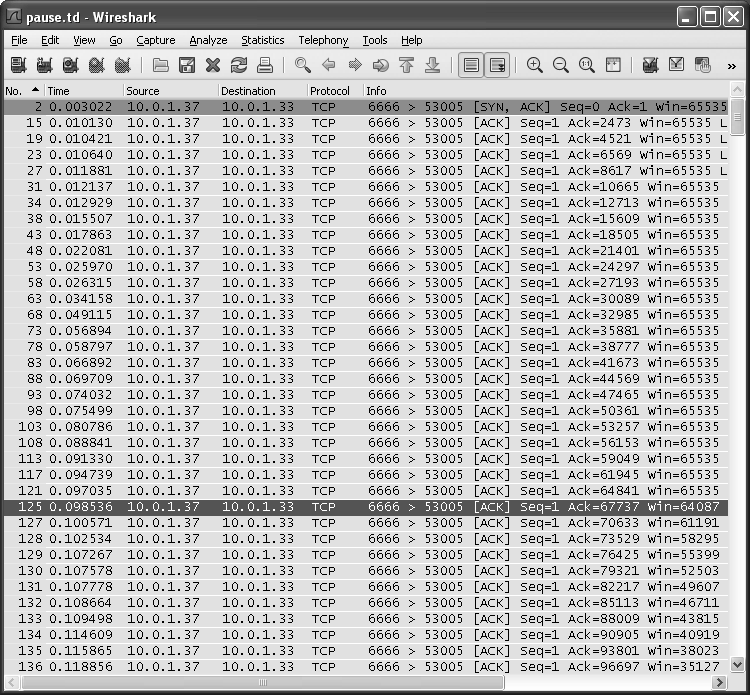
\includegraphics[width=0.7\textwidth]{imgs/15/15-11.png}
	\caption{比较相似环境下使用 Nagle算法与否的延}
\end{figure}
从图15-11 中可以看到,在接收了100多个包后,窗口大小仍然维持在64KB。这是由于自动窗口调节算法(参见 15.5.4节)默认分配了 TCP 接收端的缓存。然而,随着可用缓存
的减少,可以看到在125号包之后,窗口开始减小。随着大量的ACK 到达,窗口进一步减小,每个到达的ACK 号都增大2896字节。这表明接收端在存储这些数据,但应用程序并没
有处理。如果我们进一步观察,会发现最终接收端已经没有更多空间来存储到达的数据(见图 15-12)。

从图15-12 中可以看到,151号包耗尽了 327字节大小的窗口,Wireshark 显示“TCP窗口满”(TCP Window Full)。约200ms后,在4.979s时刻,零窗口通告产生,表明无法接
收新的数据。窗口最后的可用空间已满,接收端应用程序暂停处理数据,直到20.143s时刻。

收到零窗口通告后,发送端每隔5s共发送了三次窗口探测以查看窗口是否打开。在20s时刻,接收端开始处理 TCP 队列中的数据。因此有两个窗口更新传送至发送端,表明可以
继续传输数据(64KB)。窗口更新并不是对新数据的确认,而只是将的日右边界有弦。这时,发送端可以恢复正常的数据传输。

随着接收端可用缓存的逐渐减小,在一段时间后,窗口开始减小。如果接收端应用程序一直不处理任何数据,且发送端持续发送,窗口最终会缩减为0
\begin{figure}[!htb]
    \centering
	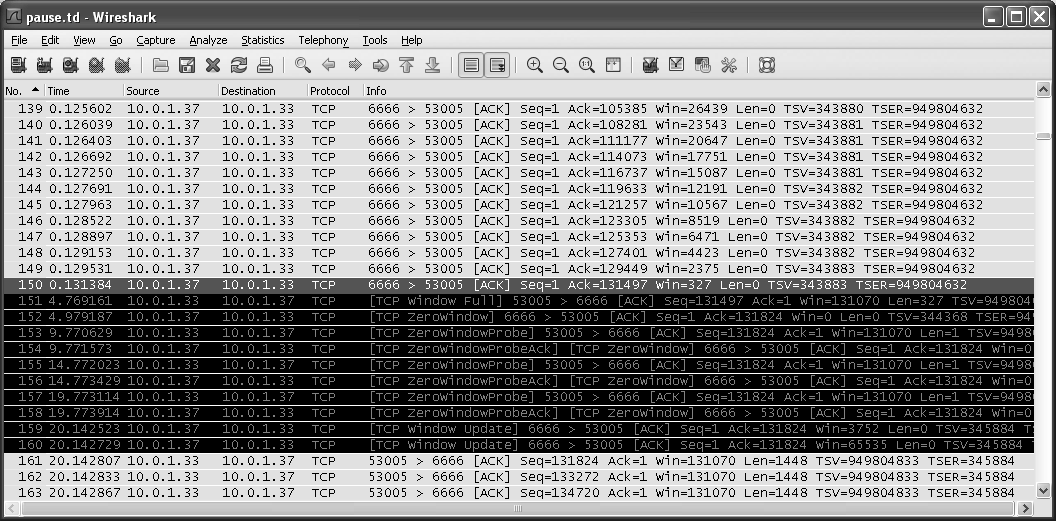
\includegraphics[width=0.7\textwidth]{imgs/15/15-12.png}
	\caption{接收端缓存已满。当接收应用程序再次开始处理数据时,窗口更新会通知发送端可继续发送}
\end{figure}

从图15-11 和图15-12中可以总结出以下几点:
\begin{enumerate}
    \item 发送端不必传输整个窗口大小的数据。
    \item 接收到返回的 ACK 的同时可将窗口右移。这是由于通告窗口是和该报文段中的ACK号相关的。
    \item 窗口大小可能减小,如图15-11所示,但窗口右边界不会左移,以此避免窗口收缩。
    \item 接收端不必等到窗口满才发送 ACK。
\end{enumerate}

此外,还可通过观察吞吐量随时间的变化函数得到一些启发。使用 Wireshark的“统计|TCP 流图|吞吐量图”(Statistics | TCP Stream Graph | Throughput Graph) 功能,可以得到图
15-13 所示的时间序列。
\begin{figure}[!htb]
    \centering
	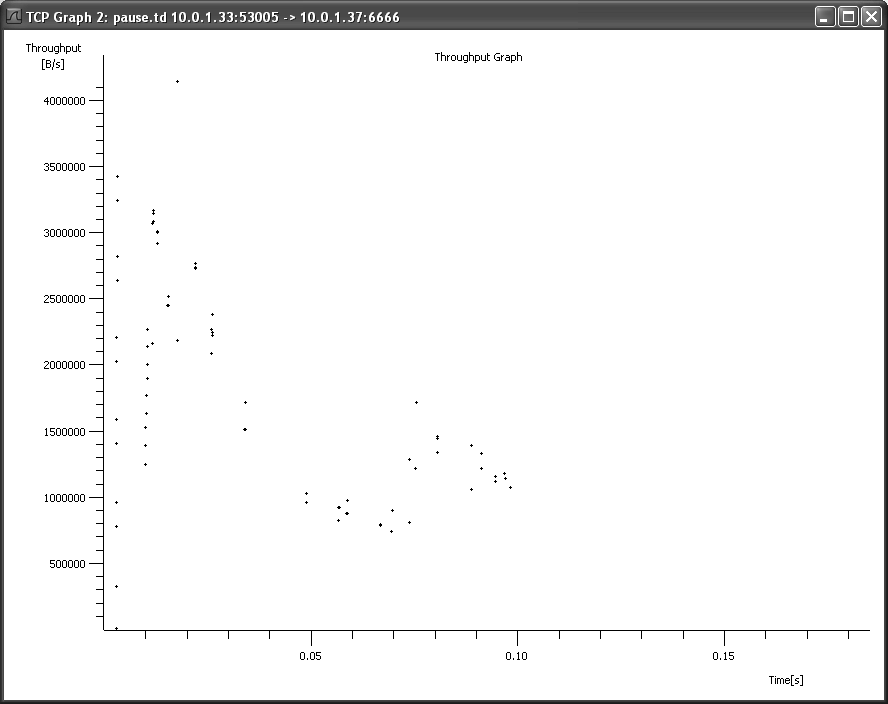
\includegraphics[width=0.7\textwidth]{imgs/15/15-13.png}
	\caption{使用相对较大的接收缓存,即使在接收端应用处理数据前也能传输大量的数据}
\end{figure}

这里我们看到一个有趣的现象。即使在接收端处理任何数据前,连接依然能达到约1.3MB/s的吞吐量。这种状况一直持续到约0.10s时刻。之后,直到接收端开始处理数据前
(在20s时刻后),吞吐量基本上都为0。

\subsection{糊涂窗口综合征}
基于窗口的流量控制机制,尤其是不使用大小固定的报文段的情况(如 TCP),可能会出现称为糊涂窗口综合征(Silly Window Syndrome,sws)的缺陷。当出现该同题时,交换
数据段大小不是全长的而是一些较小的数据段[RFC0813]。由于每个报文段中有用数据相对于头部信息的比例较小,因此耗费的资源也更多,相应的传输效率也更低。

TCP 连接的两端都可能导致SWS 的出现:接收端的通告窗口较小(沒有等到窗口变大才通告),或者发送端发送的数据段较小(没有等待将其他数据组合成一个更大的报文段)。
要避免 SWS 问题,必须在发送端或接收端实现相关规则。TCP 无法提前预知某一端的行为。需要遵循以下规则:
\begin{itemize}
    \item 对于接收端来说,不应通告小的窗口值。[RFC1122]描述的接收算法中,在窗口可增至一个全长的报文段(即接收端 MSS)或者接收端缓存空间的一半(取两者中较小者)之前,不能通告比当前窗口(可能为0)更大的窗口值。注意到可能有两种情况会用到该规则:当应用程序处理接收到的数据后使得可用缓存增大,以及 TCP接收端需要强制返回对窗口探测的响应。
    \item 对于发送端来说,不应发送小的报文段,而且需由Nagle 算法控制何时发送。为避免SWS 问题,只有至少满足以下条件之一时才能传输报文段:
    \begin{itemize}
        \item 全长(发送 MSS 字节)的报文段可以发送。
        \item 数据段长度≥接收端通告过的最大窗口值的一半的,可以发送。
        \item 满足以下任一条件的都可以发送:(i)某一ACK 不是目前期盼的(即没有未经确认的在传数据);(ii)该连接禁用 Nagle 算法。
    \end{itemize}
\end{itemize}

条件(a)最直接地避免了高耗费的报文段传输问题。条件(b)针对通告窗口值较小,可能小于要传输的报文段的情况。条件(c)防止TCP 在数据需要被确认以及 Nagle 算法启
用的情况下发送小报文段。若发送端应用在执行某些较小的写操作(如小于报文段大小),条件(c)可以有效避免SWS。

上述三个条件也让我们回答了以下问题:当有未经确认的在传数据时,若使用Nagle 算法阻止发送小的报文段,究竟多小才算小?从条件(a)可以看出,“小”意味着字节数要小
于 SMSS(即不超过 PMTU 或接收端MSS 的最大包大小)。条件(b)只用于比较旧的原始主机,或者因接收端缓存有限而使用较小通告窗口时。

条件(b)要求发送端记录接收端通告窗口的最大值。发送端以此猜测接收端缓存大小。尽管当连接建立时缓存大小可能减小,但实际这种情况很少见。另外,前面也提到过,TCP
需要避免窗口收缩。

\subsubsection{例子}
下面我们通过一个具体的例子来观察SWS避免的行;本例也包含持久计时器。这里使用我们的sock 程序,发送端主机为 Windows XP 系统,接收端为 FreeBSD,执行三次
2048字节的写操作传输。发送端命令如下:
\begin{verbatim}
    C:\> sock -1 -n 3 -W 2048 10.0.0.8 6666
\end{verbatim}
接收端相应的命令为:
\begin{verbatim}
    FreeBSD& sock -i -s -P 15 -p 2
-× 256
-R 3000 6666
\end{verbatim}

该命令将接收端缓存设为3000字节,在首次读数据前有15s的初始延时,之后每次读都会引入2s的延时,每次读的数据量为256字节。设置初始延时是为使接收端缓存占满,
最终迫使传输停止。这时通过使接收端执行小的读操作,我们期望看到它执行SWS避免。利用 Wireshark 可以得到如图15-14所示的记录。

整个连接的传输内容如图所示。包长度是根据每个报文段中携带的 TCP 有效载荷数据描述的。在连接建立过程中,接收端通告窗口为3000字节,MSS为1460字节。发送端在
0.052s时刻发送了一个 1460字节的包(包4),在0.053s时刻发送了588字节的包(包5)。两者总和为 2048字节,为应用写操作的大小。包6是对这两个包的确认,并提供了一个952
字节的窗口通告(3000-1460-588=952)。
\begin{figure}[!htb]
    \centering
	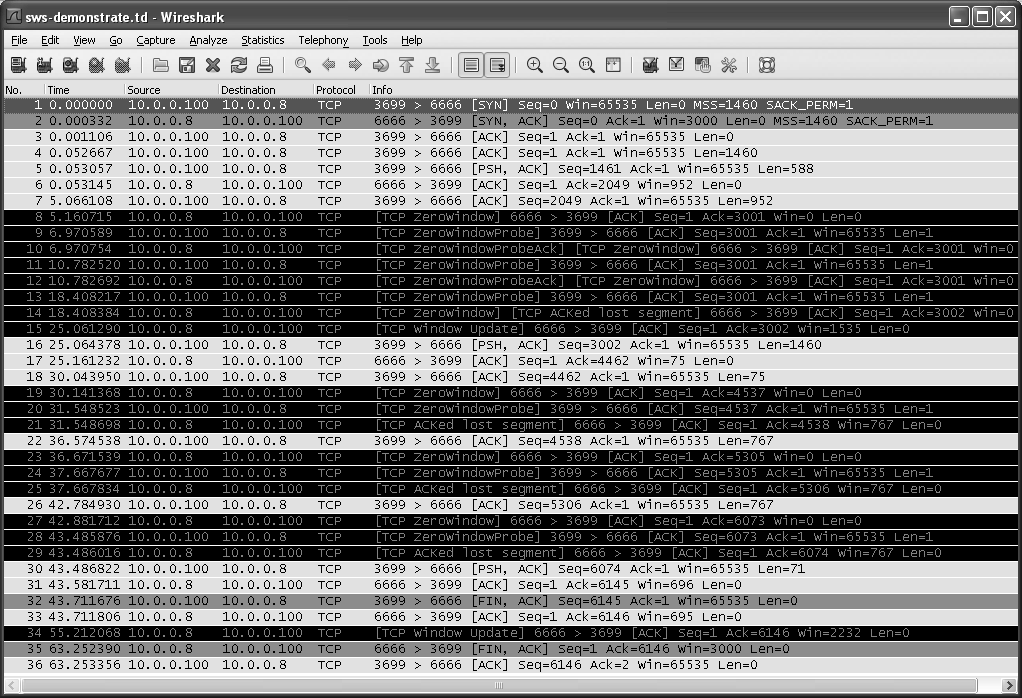
\includegraphics[width=0.7\textwidth]{imgs/15/15-14.png}
	\caption{SWS避免的行为分析。由于在0.0538时刻执行SWS 避免,发送端没有使用通告窗口传输数据。相反,一直等到5.066s 时刻,同时也有效地执行了窗口探测。通过14号包可以看到接收端SWS避免,即使已经处理了部分数据,接收端依然通告零窗口}
\end{figure}

952 字节的窗口(包6)并没有一个 MSS大,所以Nagle 算法阻止了发送端的立即发送。相反,发送端等待了 5S,直到特续计时器超时,才发送了一个窗口探测。考虑到无论如
何都要发送一个包,因此发送端发送了允许的952 字节数据填满了可用窗口,因此包8返回了零窗口通告。

下一个事件发生在6.970s时刻,TCP发送了一个窗口探测,即在接收到首个零窗口通告约25后。探测包本身包含一个字节的数据,图中 Wireshark显示为“TCP Zero WindowProbe",
但对该探测包的 ACK 号却没有增大(Wireshark 将其标记力“TCP Zero WindowProbeAck”),因此这一个字节的数据并没有被接收端保存。在10.7828时刻又产生了一个探测包(约45后),
接着 18.408s 时刻又产生一个(约8s以后),表明其发送间隔随时间呈指数增长。注意到最后一次窗口探测中包含的一个字节的数据已被接收端确认。

在25.061s时刻,在上层应用执行了6次256字节的读数据操作后(每次同隔25),窗口更新表明现在接收端缓存中有 1535字节(ACK 号加1)的可用空间。根据接收端SWS避
免规则,该数位已“足够大”。发送端开始继续传送数据。在25:0645 时刻发送了1400字节的包,在25.161s 时刻得到了对 4462 字节数据的 ACK,这时通告窗口大小只有75字节(包
17)。该通告似乎违背了我们之前的规则,即窗口值应至少为一个 MSS(对FreeBSD 来说)或总级存空间的四分之一。出现这种情况的原因在于避免窗曰收缩。最后一个窗口更新中
(包15),接收端通告窗口右边界为(3002+ 1535)-4537。如果当前ACK(包17)通告的窗日小于75字节,像接收端SWS 避免要求的那样,窗口右边界就会左移,TCP是不允许出现
这种情况的。因此这 75字节的通告窗口代表一种更高的优先级:避免窗口收缩优先于避免SWS。

通过包17和包18之间的5s的延时,我们再次看到发送端的SWS避免。发送端被强制要求发送一个75字节的包,接收端返回一个零窗口通告响应。在1s之后的包20是再次的
窗口探测,得到了767字节的可用窗口。又一轮的发送端SWS避免导致了Ss的延时;发送端填满窗口后,再次返回零窗口通告;这种状况一直重复。最终发送端没有新的数据发送而
终止。包30代表发送的最后一个包,在20s后连接终止(由于接收端应用每次读数据的间隔为2s)。

为了理解上层应用行为、通告窗口和SWS避免之间的关系,我们将连接的动态传输以表格的形式展现出来。表15-1 给出了发送端和接收端的行为,以及接收端应用执行读操作
的估计时间。

SWS 避免的通告窗口及应用层动态变化情况


在表15-1中,第1列表示图中出现的每个传输行为的相对时刻,带三位小数的数值是Wireshark 显示的时间值(参见图15-14)。而不带小数的则是接收端主机行为的估计时刻,
图中并没有显示。

接收端缓存中的数据(表中标记为“已存数据”)随着新数据的到达而增加,随着上层应用的读取而减少。我们想了解的是接收端返回给发送端的窗口通告中包含的内容。这样就
能知道接收端是怎样避免SWS的。

如前所述,第一次SWS避免是包6和包7之间的5s延时,由于窗口大小只有952字节,发送端一直避免传输直到被强制要求发送数据。传输完成后,接收端缓存满,之后产生
了一系列的零窗口通告和窗口探测交换。我们可以看到持续计时器指示的时间间隔星指数增长:探测包的发送时刻为6.970s,10.782s和18.408S。这些时刻与发送端首次接收到零窗口
通告的时刻5.160s 的间隔约为2S、4s、8S。

尽管上层应用在15s和17s时刻读数据,但至18.408s时刻为止只读了512字节。根据接收端SWS 避免规则要求,由于512字节的可用缓存既小于总缓存空间(3000字节)的一
半,也没有达到一个 MSS(1460字节),因此不能提供窗口更新。发送端在 18.408s时刻发送了一个窗口探测(报文段13)。该探测包被接收,由于缓存有一定的可用空间,因此其中
包含的一个字节数据也被保存,报文段12和14之间的ACK号的增长验证了这一点。

尽管有511字节的可用空间,但接收端再次实施了SWS 避免。接收端 FreeBSD 在实现sWS避免时区分了何时发送窗口更新与怎样响应窗口探测。它遵循[RFC1122] 中的规则,
只在通告窗口至少为总接收缓存的一半(或一个 MSS)时才发送窗口更新,并且只有当窗口至少为一个 MSS 或超过总接收缓存的四分之一才响应窗口探测。但在这里,511字节小于一
个 MSS 且不到3000/4=750字节,因此接收端只好对报文段13的ACK 中包含的通告窗口设为0。

直到25 时刻为止,上层应用完成了6次读操作,接收端缓存有 1535字节空闲(大于总的3000字节的一半),因此发送了一个窗口更新(报文段15)。发送的数据为全长报文段
(报文段16),接收到的ACK 中包含的通告窗口仅为75字节。在接下来的5S内,两端都执行SWS 避免。发送端需要等待一个更大的通告窗口,上层应用在27s时刻和 29s时刻执行
读操作,但只有587 字节的空间,不足以发送窗口更新。因此,发送端持续等待了 Ss并最终发送了剩余的75字节,迫使接收端再次进入SWS避免状态。

接收端没有提供窗口更新,直到31.548s时刻发送端的持续计时器超时,发送了一个窗口探测。接收端响应了一个非零窗口,为767 字节(大于总接收级存的四分之一)。该窗口值
对发送端并非足够大,因此继续执行发送端的SWS 避免。发送端等待了SS,之后一直重复上述过程。最终,在43.486s 时刻,最后的71字节发送完并得到确认。该 ACK 中包含696字节
的窗口通告。尽管小于总接收缓存的四分之一,为了避免窗口收缩,通告窗口并没有设为0。

从报文段32开始,不再包含数据,连接开始关闭。随即得到的确认中窗口大小为695字节(接收端的FIN消耗了一个序列号)。在上层应用再次完成6次读操作后,接收端提供
了一个窗口更新,但发送端已经完成所有数据的发送,并保持空闲状态。上层应用又执行了4次读操作,其中3次返回256字节,最后1次没有返回,表明已经无数据到达。此时,接
收端关闭连接并发送 FIN。发送端返回了最后一个 ACK,双向连接结束。

由于发送端应用在执行3次2048字节的写操作后开始关闭连接,在发送完报文段32后,发送端从 ESTABLISHED 状态变为 \verb|FIN_WAIT_1| 状态(参见第13章)。接着在接收到报
文段33后,进入\verb|FIN_WAIT_2|状态。尽管在这时接收到了窗口更新,但发送端没有任何动作,因为它已经发送了 FIN并经确认(这一阶段没有计时器)。相反,在接收到对方的FIN
前,它只是静静等待。这就是我们没有看到更多的传输直至接收到FIN 的原因(报文段35)。

\subsection{大容量缓存与自动调优}
从前面的章节可以看到,在相似的环塊下,使用较小接收缓存的 TCP 应用的吞吐性能更差。即使接收端指定一个足够大的级存,发送端也可能指定一个很小的缓存,最终导致性
能变差。这个问题非常严重,因此很多 TCP 协议栈中上层应用不能指定接收缓存大小。在多数情况下,上层应用指定的级存会被忽视,而由操作系统来指定一个较大的固定值或者动
态变化的计算值。

在较新的 Windows版本(Vista/7)和Linux 中,支持接收窗口自动调优[S98]。有了自动调优,该连接的在传数据值(连接的带宽延时积———个重要概念,将在第16章讨论)需
要不断被估算,通告窗口值不能小于这个值(假如剩余缓存空间足够)。这种方法使得TCP达到其最大可用吞吐率(受限于网络可用容量),而不必提前在发送端或接收端设置过大的级
存。在 Windows 系统中,默认自动设置接收端缓存大小。然而,也可以通过 netsh 命令更改默认值:
\begin{verbatim}
    C: \> netsh interface tcp
set heuristics disabled
C:\> netsh interface tcp set global autotuningleve1=x
\end{verbatim}

这里X可设置力 disabled、highlyrestricted、restricted、normal 或 experimental。不同的设置值会影响接收端通告窗口的自动选择。在disabled 状态下,禁用自动调优,窗口大小使
用默认值。restricted 模式限制窗口增长,normal 允许其相对快速增长。而 experimental 模式允许窗口积极增长,但通常并不推荐normal模式,因为许多因特网站点及某些防火墻会干
扰,或没有很好地实现 TCP 窗口缩放(Window Scale)选项。

对于 Linux 2.4及以后的版本,支持发送端自动调优。2.6.7及之后的版本,两端都支持该功能。然而,自动调优受制于缓存大小。下面的 Linux sysctl 变量控制发送端和接收端的
最大缓存。等号之后的值为默认值(根据不同的Linux 版本可能会有不同),如果系统用于高带宽延时积的环境下,上述值需要增大。

\begin{verbatim}
    net.core.rmem_max = 131071
net.core.wmem_max = 131071
net.core.rmem_default = 110592
net.core.wmem_default = 110592
\end{verbatim}

另外,通过下面的变量设定自动调优参数:
\begin{verbatim}
    net. ipv4.tep_rmem = 4096 87380 174760
net.ipv4.tcp_wmem = 4096 16384
131072
\end{verbatim}

每个变量包含三个值:自动调优使用的缓存的最小值、默认值和最大值。
\subsubsection{例子}
为演示接收端自动调优行为,这里采用Windows XP 发送端(设为使用大容量窗口和窗口缩放)和Linux 2.6.11 接收端(支持自动调优)。在发送端运行如下命令:
\begin{verbatim}
    C:\> gock -n 512 -1 10.0.0.1 6666
\end{verbatim}

对接收端,我们不对接收级存做任何设置,但在上层应用读取数据前设置20s的初始延时:
\begin{verbatim}
    Linux8 sock -1 -g -v -₽ 20 6666
\end{verbatim}

为描述接收端通告窗口的增长,可以利用Wireshark 来显示包传输情况,并根据接收端地址来进行分类(参见图15-15)。在连接建立阶段,接收端初始窗口值为1460字节,初始
MSS 为1412字节。由于其采用了窗口缩放,会有2倍的变动(图中没有显示),使得最大可用窗口为256KB。可以看到在完成第一个包传输后,窗口有了增长,相应地发送端也提高了
发送速率。在第16章中我们将会讨论 TCP拥塞控制的发送速率。现在,我们只需要知道发送端何时开始发送,通常情况下其首先发送一个包,接着每收到一个ACK,发包数就增加
一个 MSS。因此,每接收一个 ACK,就会发送两个包(每个包长度为一个 MSS)。
\begin{figure}[!htb]
    \centering
	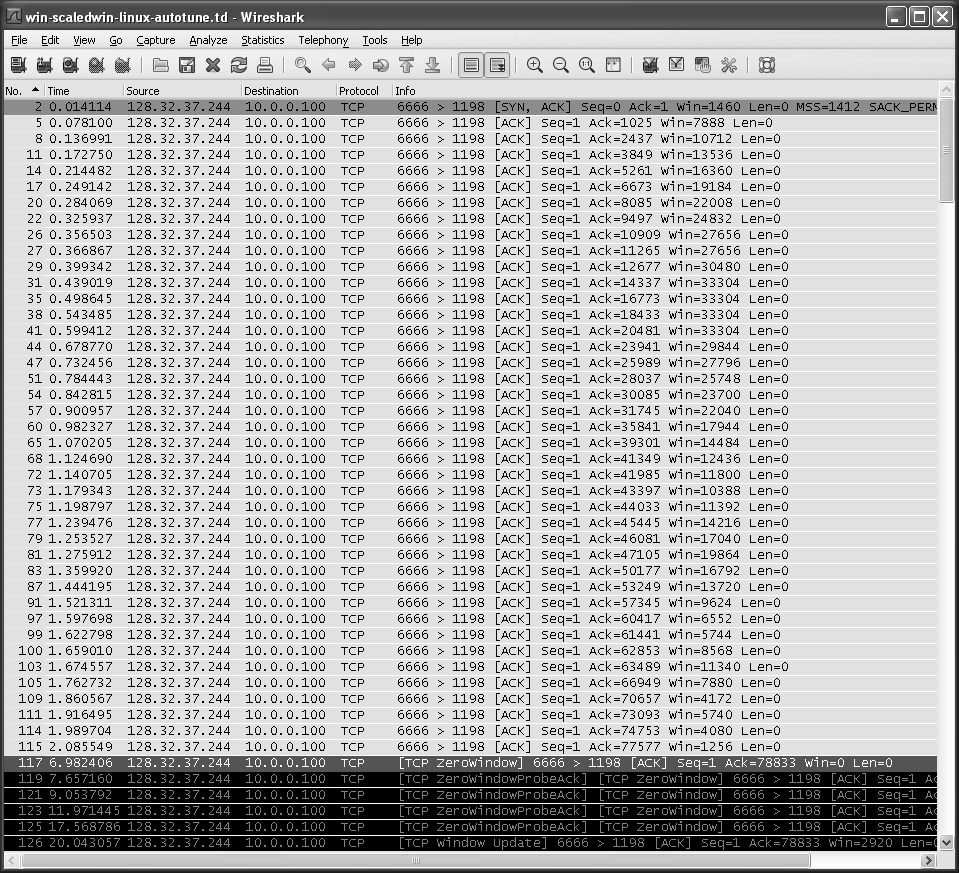
\includegraphics[width=0.7\textwidth]{imgs/15/15-15.png}
	\caption{Linux 接收端执行自动调优,窗口值随着接收数据的增多而增大。由于上层应用在20s之内都没有读取数据,最终窗口将关闭}
\end{figure}

观察窗口通告值 10712、13536、16360、19184 •••可以发现,每接收一个ACK,窗口就增长两个 MSS,这与发送端拥塞控制操作相一致(第16 章会讨论)。假设接收端存储空
间足够大,根据拥塞控制局限性,通告窗口总是大于允许发送的数据量。这种方式是最优的一-在保持发送端最大发送速率的情况下,接收端通告和使用的缓存空间最小。

当接收端缓存资源耗尽时,自动调优也会受影响。在本例中,0.678s时刻窗口达到最大值33304字节,接着开始减小。这是由于上层应用停止读取数据,导致缓存被占满。当20s
后上层应用继续读操作时,窗口再次增大,并超过了之前的最大值(参见图15-16)。
\begin{figure}[!htb]
    \centering
	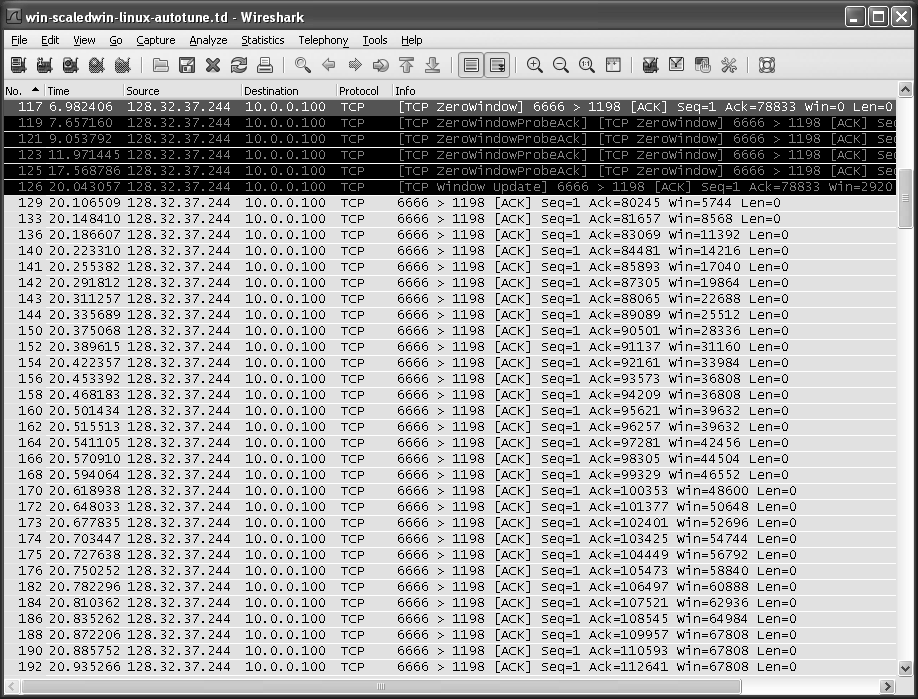
\includegraphics[width=0.7\textwidth]{imgs/15/15-16.png}
	\caption{当上层应用暂停读取数据时,接收端缓冲区开始被占满,自动调优也相应停止。随着读操作的继续执行,通告窗口也逐渐增大,并超过了之前的最大值}
\end{figure}

零窗口通告(包 117)使得发送端执行了一系列的窗口探测,但返回的仍是一系列的零窗口。在 20.043s时刻恢复读数据操作时,发送端接收到了窗口更新。每接收到一个ACK,
窗口就增大两个 MSS。随着数据的发送、接收和处理,通告窗口达到了最大值67808。该版本的Linux 也测量相邻两次读操作完成的时间,并与估计 RTT值相比较。如果 RTT 估计值
增大,那么缓存也将增大(但不会因 RTT 的减小而减小缓存)。这样即使在连接的带宽延时积增大的情况下,自动调优也保持接收端通告窗口优先于发送端窗口。

随着广域网络连接速度的增长,TCP 应用使用的缓存太小已成为严重局限。在美国,全国范围内的RTT约为 100ms,在一个1Gb/s的网络中使用64KB的窗口将 TCP 吞吐量限制
在约640KB/s,而计算的最大值可以达到约130MB/s(99\%的带宽都浪费了)。实际上,如果在相同网络环境下使用较大容量的缓存,吞吐性能将提升100倍。Web100工程[W100]应
得到更多关注和信心。它开发了一系列工具和改进软件,致力于使应用从众多的TCP 实现中获得最优的吞吐性能。

\section{紧急机制}
我们在第12章中已经提到,TCP头部有一个位字段URG用来指示“紧急数据”。应用在执行写操作时,可通过设置 Berkeley 套接字 API(\verb|MSG_00B|)的特殊选项将数据标记
为紧急,但[RFC6093]不再推荐设置紧急数据。当发送端 TCP收到这类写操作要求时,会进入称为紧急模式(urgent mode)的特殊状态。它记录紧急数据的最后一个字节,用于设
置紧急指针(Urgent Pointer)字段,随后发送端生成的每个 TCP头部都包含该字段,直到应用停止紧急数据写操作,并且所有序列号在紧急指针之前的数据都经接收端确认。根据
[RFC6093],紧急指针指示的是紧急数据之后的一个字节。大量的 RFC文档中对紧急指针的阐述都存在语义上的模糊和二义性。对于使用IPv6 的超长数据报而言,紧急指针值需设为
65535,用于指示紧急数据的末端位于 TCP数据域的最后[RFC2675],如果使用传统的16位紧急指针字段就不能表示 64KB的偏移。

当收到UGR 置位的报文段时,TCP 接收端就会进入紧急模式。接收端应用可以调用标准套接字 API (select O)来判断是否进入紧急模式。紧急机制会带来操作上的混淆,因为
Beikeley 套接字 API 和文档中用到了术语:带外(Out-Of-Band, 0OB)数据。而实际上TCP并没有实现任何OOB 功能。相反,差不多所有 TCP实现在将紧急数据的最后一个字节传输
给上层应用时,在接收端使用了一个截然不同的API 参数。接收端必须要设置 \verb|MSG_OOB|选项检索该字节,或者设置 \verb|MSG_OOBINLINE| 使该字节保持在正常数据流传输(在使用紧
急机制情况下,需要用到该方法)。

\subsection{例子}
为更好地理解紧急机制,我们通过一个例子来具体观察紧急模式的行为,包括在零窗口事件期间发生的状况。这里使用 Mac OS X 发送端和Linux 接收端。为获得零窗口,我们首
先在接收端限制接收窗口自动调优:

\begin{verbatim}
    Linux# sysctl -w net. ipv4.tcp_rmem='4096 4096 174760'
    Linux& sock -1 -v -в -D 1 -P 10 5555
\end{verbatim}

第一个命令确保接收窗口的自动调整幅度不超过4KB,这样就可以清楚地看到窗口关闭时发生的情形。第二个命令使服务器在读数据前等待 10s,并在每次读操作间等待1s。在客
户端我们执行如下命令:
\begin{verbatim}
    Mac& sock -1 -n 7 -0 7 -D1 -8 8192 10.0.1.1
SO_SNDBUF
5555
- 8192
connected on 10.0.1.33.51101 to 10.0.1.1.5555
TCP_MAXSEG = 1448
wrote 1024 bytes wrote 1024 bytes wrote 1024 bytes wrote 1024 bytes wrote 1024 bytes wrote 1024 bytes
wrote 1 byte of urgent data
wrote 1024 bytes
\end{verbatim}

该命令使得客户端每隔1s执行一次写操作,共7次,每次1024字节,且在最后一次写之前写了1个字节的紧急数据。客户端级存设置为 8192 字节,由于在TCP 发送数据前所有
数据都暂时存储在发送端,因此缓存已足够大,该应用可立即得到执行。

如图 15-17所示,接收端初始通告窗口右边界为 2800,并很快增至5121。在1.0s时刻,应用执行了一次写操作,窗口有边界前进至6145。之后由于自动调优在高于4192 字节时被
禁用且接收应用没有执行读操作,窗口没有继续增长。直到10.0s时刻,发送端执行了窗口探测,但依旧没有获得窗口增长。最终在 10.0s 时刻之后,接收端开始继续读取数据,窗口
打开,发送端继续发送直至完成传输。包交换情况如图15-18所示。
% \begin{figure}[!htb]
%     \centering
% 	\includegraphics[width=0.7\textwidth]{imgs/15/15-17.png}
% 	\caption{在执行6次写操作后,接收端窗口没有前移。TCP发送端暂停发送,直至在10s时刻窗口打开}
% \end{figure}

紧急模式的“出口点”定义为TCP报文段中序列号字段与紧急指针字段之和。每个TCP 连接只维护一个紧急“点”(序列号偏秘),因此紧急指针字段为空的包会导致前面的紧
急指针包含的信息丢失。报文段16为第一个包含有效紧急指针的报文段,使得序列号 6146到达出口点。注意到该序列号可能并不在指示的报文段中,而可能在之后的报文段中。例如
报文段17就是这种情况,它没有包含任何数据,只有紧急指针(值为1)。

如前所述,有个问题一直存在争议,即出口点指示的是紧急数据的最后一个字节还是非紧急数据的第一个字节。TRFCI122]认为指针指示的是紧急数据的最后一个字节。然而,基
本上所有的TCP实现都没有遵循该规定,因此[RFC6093]认识到了这一问题,并修改规范让指针指向非紧急数据的第一个字节。在本例中,序列号为6145的字节包含工由sock 客户
瑞产生的】字节紧急数据,但在所有的报文段中,紧急指针的信为1,序列号为6145。因此,可以看出该 TCP 实现中(大多数 TCP 实现都如此),出口点为非紧急数据的第一个字节
的序列号。
\begin{figure}[!htb]
    \centering
	\includegraphics[width=0.7\textwidth]{imgs/15/15-18.png}
	\caption{整个数据传输在5.0125时刻出现了一次零窗口通告。当应用执行下一次写操作时,发送端TCP 进入紧急模式,6.0113s时刻发送的窗口探测报文段中的URG置位。
    在第7秒执行最后一次写操作并关闭,产生了两个空的报文段。10.006s时刻的窗口更新重新启动数据传输。10.009s时刻的零窗口通告使得传输再次停止,同时由于紧急指针已被确认,
    因此可以退出紧急模式。11.007s时刻的FIN 包含了数据的最后一个字节}
\end{figure}
从这个例子可以看到,TCP将紧急数据携带在数据流中传输(而非“带外传输”)。如果某个应用确实需要独立的信号通道,可以简单采用另一个 TCP 连接。(某些传输层协议确实
提供大多数人认为的OOB 数据,即像通常数据链路那样使用同一个连接,但有独立的逻辑数据路径。TCP 并不提供该功能。)


\section{与窗口管理相关的攻击}
TCP 窗口管理可能受到多种攻击,主要形式为资源耗尽。通告窗口较小会使得TCP传输减慢,因此会更长时间地占用资源,如存储空间。这一点已被用于针对传输性能较差的网
络攻击(即蠕虫)。例如,LaBrea tarpit程序[LO1]在完成 TCP 三次握手后,要么不做任何行为,要么只产生一些最小的应答,使得发送速率不断减慢。通过此法来保持发送端忙碌,本
质上是减慢蜗虫的传播速度。因此 tarpit 程序是针对流量攻击的一类攻击。

比较新的攻击发布于2009年[109],它基于已知的持续计时器的缺陷,采用客户端多“SYN cookies” 技术(参见第13章)。所有必要的连接状态都可以下载到受害主机进
行,从而使得攻击方主机消耗最少的资源。这种攻击本身类似于LaBrea 思想,只是其针对持续计时器。同一台服务器可能受到多个此类攻击,最终导致资源耗尽(如系统内存耗
尽)。[C723308] 提出了一种解决方法,即当推断出现资源耗尽时,允许其他进程关闭TCP连接。


\section{总结}

交互式数据传输的报文段通常小于SMSS。接收方收到这些分组时可能会采取延时确认的方法,希望能将这些 ACK与需要发送给对方的数据一起捎带传输。这种方法可以减少传
输报文段的数目,特别是在交互式流量传输中,服务器需要对客户端的每个按键都返回响应。然而,延时确认也会引人额外的延时。

对于RTT 相对较大的连接,如WAN,通常使用Nagle算法来减少较小报文段数目。该算法限制发送端在任意时刻发送单个小数据包。这样会减少较小数据包在网络连接中的
数目,从而减小传输资源开销,但同时也可能引人上层应用无法接受的延时。另外,延时ACK与Nagle算法的互相作用可能导致短暂的死锁。基于上述原因,有的应用可能禁用
Nagle算法,而大多数交互式应用都使用该功能。

TCP通过在其发送的每个 ACK 中包含一个窗口通告来实现流量控制。该窗口告诉对方自己还有多少缓存空间。当没有使用 TCP 窗口缩放选项时,最大通告窗口为65535字节。
否则最大窗口值可以更大(约1GB)。

通告窗口值可能为0,表明接收端缓存已满。这时发送端停止发送,并以一定间隔不断地发送窗口探测,发送间隔类似于超时重传(参见第14章),直到收到ACK 表明窗口变大,
或收到接收端主动发送的窗口通告(窗口更新)表明有可用缓存空间。这种以一定间隔连续发送的行 可能被用于资源耗尽攻击。

随着TCP 的不断发展,出现了一种奇怪的现象。当通告窗口较小时,发送端会立即发送数据填满该窗口,这样在连接中就会出现大量高耗费的小数据包。这种现象被称为“糊涂
窗口综合征”。针对这一问题,在 TCP发送端和接收端都有相应的策略。对发送端来说,若通告窗口较小则避免发送小数据包;接收端则尽量避免通告小窗口。

接收端窗口大小受限于其缓存大小。一般来说,如果上层应用没有设置其接收缓存大小,就会为其分配一个相对较小的空间,这样即使在高带宽的传输路径上,传输延时仍旧很
大,导致网络吞吐性能变差。在较新的操作系统中不会出现上述问题,采用自动调优的方法可以高效地自动分配缓存大小。

\chapter{TCP拥塞控制}
\minitoc

\section{引言}
本章将探讨 TCP 实现拥塞控制的方法,这也是批量数据传输中最重要的。拥塞控制是TCP 通信的每一方需要执行的一系列行为。这些行为由特定算法规定,用于防止网络因为大
规模的通信负载而瘫痪。其基本方法是当有理由认为网络即将进入拥塞状态(或者已经由于拥塞而出现路由器丢包情况)时减绥 TCP传输。TCP 拥塞控制的难点在于怎样准确地判断何
时需要减缓且如何减缓 TCP 传输,以及何时恢复其原有的速度。

TCP 是提供系统间数据可靠传输服务的协议。第15章已经提到,当 TCP 通信的接收方的接收速度无法匹配发送速度时,发送方会降低发送速度。TCP 的流量控制机制完成了对发
送速率的调节,它是基于 ACK 数据包中的通告窗口大小字段来实现的。这种方式提供了明确的接收方返回的状态信息,避免接收方缓存溢出。

当网络中大量的发送方和接收方被要求承担超负荷的通信任务时,可以考虑采取降低发送速率或者最终丢弃部分数据(也可将两者结合使用)的方法。这是将排队理论应用于路由
器的基本观测结果:即使路由器能够存储一些数据,但若源源不断的数据到达速率高于发出速率,任何容量的中间存储都会溢出。简言之,当某一路由器在单位时间内接收到的数据量
多于其可发送的数据量时,它就需要把多余的部分存储起来。假如这种状况持续,最终存储资源将会耗尽,路由器因此只能丢弃部分数据。

路由器因无法处理高速率到达的流量而被迫丢弃数据信息的现象称为拥塞。当路由器处于上述状态时,我们就说出现了拥塞。即使仅有一条通信连接,也可能造成一个甚至多个路
由器拥塞。若不采取对策,网络性能将大受影响以致瘫痪。在最坏情况下,甚至形成拥塞崩溃。为避免或者在一定程度上缓解这种状况,TCP 通信的每一方实行拥塞控制机制。不同的
TCP 版本(包括运行 TCP/IP 协议栈的操作系统)采取的规程和行为有所差异。本章将着重讨论最常用的方法。
\subsection{TCP 拥塞检测}
如前所述,针对丢包情况,TCP 采取的首要机制是重传,包括超时重传和快速重传(参见第14 章)。考虑如下情形,当网络处于拥塞崩溃状态时,共用一条网络传输路径的多个
TCP 连接却需要重传更多的数据包。这就好比火上浇油,可想而知,结果只会更糟,所以这种情况应该尽量避免。

当拥塞状况出现(或将要出现)时,我们可以减缓 TCP 发送端的发送速率;若拥塞情况有所缓解,可以检测和使用新的可用带宽。然而这在互联网中却很难做到,因为对于TCP
发送方来说,没有一个精确的方法去知晓中间路由器的状态。换言之,没有一个明确的信号告知拥塞状况已发生。典型的TCP 只有在断定拥塞发生的情况下,才会采取相应的行动。
推断是否出现拥塞,通常看是否有丢包情况发生。在TCP 中,丢包也被用作判断拥塞发生与否的指标,用来衡量是否实施相应的响应措施(即以某种方式减级发送)。从20世纪80年
代起,TCP 就一直沿用这种方法。其他拥塞探测方法,包括时延测量和显式拥塞通知(ECN,16.11 节会讨论),使得 TCP能在丢包发生前检测拥塞。在学习一些“经典”算法后,我们将
讨论上述探测方法。

\begin{tcolorbox}
    在当今的有线网络中,出现在路由器或交换机中的拥塞是造成丟包的主要原因。而在无线网络中,传输和接收错误是导致丟包的重要因素。从20世纪90年代
    中期无线网络荻得广泛应用开始,判断丢包是由于拥塞引起还是传输错误引起,一直是研究的热点问题。
\end{tcolorbox}

在第14章中,我们已经看到 TCP 如何利用计时器、确认以及选择确认机制来检测丢包和恢复传输。当有丢包情况出现时,TCP的任务是重传这些数据包。现在我们关心的是,当
观测到丢包后,TCP还做了哪些工作,特别是它如何识别这就是已出现拥塞的信号,进而需要执行减速操作。下面的章节主要讨论 TCP 何时减速以及怎样减速(包括如何恢复传输速
度)。我们首先介绍 TCP 在建立新连接时如何确立基本数据传输速率,以及稳定执行大数据量传输操作的经典算法。另外,我们也整合了近年来对这些算法的研究和改进成果,并细查
了相关扩展资料。在此基础上,我们讨论总结了 TCP 拥塞控制安全和其他相关问题。拥塞控制是网络研究领域的热点[RFC6077],每年都会有相关论文发表。

\subsection{减缓TCP发送}
一个亟待解决的问题是,如何减缓TCP发送。在第15章已经提到,根据接收方剩余缓存空间大小,在TCP 头部设置了通知窗口大小字段,该数值是 TCP 发送方调节发送速率的
依据。进一步说,当接收速率或网络传输速率过慢时,我们需要降低发送速率。实现上述操作,基于对网络传输能力的估计,可以在发送端引入一个窗口控制变量,确保发送窗口大
小不超过接收端接收能力和网络传输能力,即TCP发送端的发送速率等于接收速率和传输速率两者中较小值。

反映网络传输能力的变量称为拥塞窗口(congestion window),记作cwnd。因此,发送端实际(可用)窗口 W就是接收端通知窗口 awnd 和拥塞窗口cwnd 的较小者:

\begin{equation}
    W = min (cwnd, awnd)
\end{equation}

根据上述等式,TCP发送端发送的数据中,还没有收到ACK 回复的数据量不能多于P(以包或字节为单位)。这种已经发出但还未经确认的数据量大小有时称为在外数据值(flight
size),它总是小于等于 W。通常,W可以以包或字节为单位。

\begin{tcolorbox}
    当TCP 不使用选择确认机制时,W的限制作用体现为,发送方发送的报文段序列号不能大于ACK号的最大值与 W之和。而对采用选择确认的发送方则有所
    不同,W被用来限制在外数据值。
\end{tcolorbox}

这看似合乎逻辑,但实际并非如此。因为网络和接收端状况会随时间变化,相应地,awnd 和cwnd 的数值也会随之改变。另外,由于缺少显示拥塞的明确信号(参见前述章节),
TCP发送方无法直接获得cwnd 的“准确”值。因此,变量W、cwnd、awnd 的值都要根据经验设定并需动态调节。此外,如前所述,P的值不能过大或过小—一我们希望其接近带宽
延迟积(Bandwidth-Delay Product, BDP),也称作最佳窗口大小(optimal window size)。W反映网络中可存储的待发送数据量大小,其计算值等于 RTT 与链路中最小通行速率(即发
送端与接收端传输路径中的“瓶颈”)的乘积。逼常的策略是,为使网络资源得到高效利用,应保证在网络申传输的数据量达到BDP。但若在传偷数据值远高于BDP时,会引人不必要
的延时(参见16.10节),所以这也是不可取的。在网络中如何确定一个连接的BDP是难点,需要考虑诸多因素,如路由、时延、统计复用(即共用传倫资派)水平随时间的变化性等。

\begin{tcolorbox}
    这里我们主要讨论由TCP 发送方的数据发送而产生的拥塞,但也要注意因接收方回复ACK而产生的相反方向链路上的删塞,目前也有相关研究针对孩一问
    题。在文献TRFC5690]中介绍了一种方法,该方法中TCP接收方需要很据一定比率国复ACK(即接收了多少个数据包后才能发送一个ACK)。
\end{tcolorbox}

\section{一些经典算法}
当一个新的TCP连接建立之初,还无法知获可用的传输资源,所以cwnd 的初始值也无法确定。(也有一些例外,如有些系统的缓存容量是预先设定的,在第14 章我们称其为目
的度量(destination metrie)。)TCP 通过与接收端交换一个数据包就能获得awnd 的值,不需要任何明确的信号。显而易见,获得cwnd 最佳值的唯一方法是以越来越快的速率不断发送
数据,直到出现数据包丢失(或网络阻塞)为止。这时考虑立即以可用的最大速率发送(受awnd 的限制),或是慢速启动发送。由于多个 TCP 连接共享一个网络传输路径,以全速启动
会影响其他连接的传输性能,所以通常会有特定的算法来避免过快启动,直至稳定传输后才会运行相应的其他算法。

TCP 发送方的拥塞控制操作是由ACK 的接收来驱动或“控制”的。当 TCP 传输处于稳定阶段(cwnd 取合适值),接收到 ACK 回复表明发送的数据包已被成功接收,因此可以继续
发送操作。据此推理,稳定状态下的 TCP抑塞行为,实际是试图使在网络传输路径上的数据包守恒(参见图 16-1)。这里的守恒是从物理学意义上而言的——某个量(如动量、能量)
进入一个系统不会凭室消失或出现,而是以某种表现形式继续存在。

\begin{figure}[!htb]
    \centering
	\includegraphics[width=1\textwidth]{imgs/16/16-1.png}
	\caption{TCP拥塞控制操作是基于数据包守恒原理运行的由子传输能力有限,数据包(P)会适时地“伸展”。接收方以一定问隔(P)接收到数据包后,会陆续(以4,为间隔)生成相应的
    ACK,以一定的发送间隔(小)返回给发送方。当ACK 陆线(以A.为间隔)到达发送端时,其到达提供了一个信号或者说“ACK 时钟”,表明发送嘴可以继续发送数帮。在稳定传输状
    态下,整个系统可“自同步"控制(本图改编自 [I88],源丁S. Seshan' s CMU Leeture Notes,2005.3.22)}
\end{figure}

如图16-1 所示,上下两条通道形似“漏汁”。发送方发送的(校大)数擔包经上通道传输给接收方。相对较狄窄部分表不传输较慢的连接链路,数娜包需要适时地被“伸肥”。两
端部分(位于发送方和接收方)让数据包发送前和接收后的队列。下通道传输相应ACK数据包。在高效传输的稳定状态下,上下通道都不会出现包堵塞的情况,而且在上通道中也不会
有较大传输间隔。注意到发送方接收到一个 ACK 就表明可向图16-1 中的上层通道发送一个数据包(即网络中可容纳另一个包)。这种由一个 ACK 到达(称作 ACK 时钟)触发一个新数
据包传输的关系称为自同步(sclf-clocking)。

现在我们讨论 TCP 的两个核心算法:慢启动和拥塞避免。这两个算法是基于包守恒和ACK 时钟原理,最早在 Jacobson [J88]的经典论文里被正式提出。几年后,Jacobson 对拥塞
避免算法提出了改进[J90]。这两个算法不是同时运行的—一在任一给定时刻,TCP 只运行一个算法,但两者可以相互切换。下面我们将详细讨论这两个算法,包括如何使用以及对算
法的改进。每个 TCP连接都能独立运行这两个算法。

\subsection{慢启动}
当一个新的TCP 连接建立或检测到由重传超时(RTO)导致的丢包时,需要执行慢启动。TCP 发送端长时间处于空闲状态也可能调用慢启动算法。慢启动的目的是,使TCP 在
用拥塞避免探寻更多可用带宽之前得到cwnd值,以及帮助TCP建立ACK 时钟。通常,TCP 在建立新连接时执行慢启动,直至有丢包时,执行拥塞避免算法(参见16.2.2节)进入
稳定状态。下文引自 [RFC5681]:

在传输初始阶段,由于未知网络传输能力,需要缓慢探测可用传输资源,防止短时间内大量数据注入导致拥塞。慢启动算法正是针对这一问题而设计。在数据传
输之初或者重传计时器检测到丢包后,需要执行慢启动。

TCP 以发送一定数目的数据段开始慢启动(在SYN交换之后),称为初始窗口(InitialWindow, IW)。IW 的值初始设 一个 SMSS(发送方的最大段大小),但在[RFCS681]中设
为一个稍大的值,计算公式如下:

\begin{equation}
    IW =2* (SMSS)且小于等于2个数据段(当SMSS>2190字节)
    IW =3* (SMSS)且小于等于3个数据段(当2190≥SMSS>1095字节)
    IW =4*(SMSS)且小于等于4个数据段(其他)
\end{equation}

上述 IW的计算方式可能使得初始窗口为几个数据包大小(如3个或4个),为简单起见,我们只讨论IW =1 SMSS 的情况。TCP 连接初始的cwnd =1 SMSS,意味着初始可用
窗口W也为1 SMSS。注意到大部分情况下,SMSS 为接收方的 MSS(最大段大小)和路径MTU(最大传输单元)两者中较小值。

假设没有出现丢包情况且每个数据包都有相应的ACK,第一个数据段的ACK 到达,说明可发送一个新的数据段。每接收到一个好的ACK 响应,慢启动算法会以 min (N, SMSS)
来增加 cwnd值。这里的N 是指在未经确认的传输数据中能通过这一“好的ACK”确认的字节数。所谓的“好的ACK”是指新接收的 ACK 号大于之前收到的ACK。

\begin{tcolorbox}
    已被 ACK 确认的字节数目用于支持适当字节计数(Appropriate Byte Counting,ABC)[RFC3465],这是[RFC5681]推荐的实验规范。ABC 用于计数“ACK 分裂”
    攻击(将在16.12 节叙述),指利用许多较小ACK使TCP 发送方加速发送。Linux 利用布尔系统配置变量 \verb|net.ipv4.tep_abe| 设定 ABC是否可用(默认不可用)。在最近的
    几个 Windows 版本中,ABC默认开启。
\end{tcolorbox}

因此,在接收到一个数据段的ACK后,通常 cwnd 值会增加到2,接着会发送两个数据段。如果成功收到相应的新的 ACK,cwnd 会由2变4,由4变8,以此类推。一般情况下,
假设没有丢包且每个数据包都有相应 ACK,在k轮后W的值为W=2’,即k=10g2W,需要K个 RTT 时间操作窗口才能达到 W大小。这种增长看似很快(以指数函数增长),但若与一
开始就允许以最大可用速率(即接收方通知窗口大小)发送相比,仍显缓慢。(W不会超过awnd。)

如果假设某个 TCP 连接中接收方的通知窗口非常大(比如说,无穷大),这时 cwnd 就是影响发送速率的主要因素(设发送方有较大发送需求)。如前所述,cwnd 会随着 RTT 呈指数
增长。因此,最终 cwnd(W也如此)会增至很大,大量数据包的发送将导致网络瘫痪(TCP吞吐量与 W/RTT 成正比)。当发生上述情况时,cwnd 将大幅度减小(减至原值一半)。这是
TCP 由慢启动阶段至拥塞避免阶段的转折点,与cwnd 和慢启动圖值(slow start threshold,ssthresh)相关。

图16-2(左)描述了慢启动操作。数值部分以 RTT 为单位。假设该连接首先发送一个包(图上部),返回一个 ACK,接着在第二个 RTT 时间里发送两个包,会接收到两个ACK。
TCP 发送方每接收一个ACK 就会执行一次cwnd 的增长操作,以此类推。右图描述了 cwnd随时间增长的指数函数。图中另一条曲线显示了每两个数据包收到一个ACK 时 cwnd 的增长
情况。通常在 ACK 延时情况下会采用这种方式,这时的 cwnd 仍以指数增长,只是增幅不是很大。正因 ACK 可能会延时到达,所以一些 TCP 操作只在慢启动阶段完成后才返回ACK。
Linux 系统中,这被称为快速确认(“快速 ACK 模式”),从内核版本2.4.4开始,快速确认一直是基本 TCP/P 协议栈的一部分。

\begin{figure}[!htb]
    \centering
	\includegraphics[width=0.7\textwidth]{imgs/16/16-3.png}
	\caption{经典慢启动算法操作。在没有 ACK 延时情况下,每接收到一个好的ACK 就意味着发送方可以发送两个新的数据包(左)。这会使得发送方窗口随时间垦指数增长(右,上方曲线)。当发生
    ACK 延时,如每脂一个數据包生成一个ACK, cwnd 仍3以、指数增长,但增幅较小(右,下方曲线)}
\end{figure}

\subsubsection{拥塞避免}
如上所述,在连接建立之初以及由超时判定丢包发生的情况下,需要执行慢肩动操作。在慢启动阶段,cwnd 会快速增长,帮助确立一个慢启动阈值。一旦达到阈值,就意味着可
能有更多可用的传输资源。如果立即全部占用这些资源,将会使共享路由器队列的其他连接出现严重的丢包和重传情况,从而导致整个网络性能不稳定。

为了得到更多的传输资源而不致影响其他连接传输,TCP 实现了拥塞避免算法。一旦确立慢启动阈值,TCP 会进入拥塞避免阶段,cwnd 每次的增长值近似于成功传输的数据段大小。
这种随时间线性增长方式与慢启动的指数增长相比级慢许多。更准确地说,每接收一个新的ACK, cwnd 会做以下更新:
\begin{equation}
    cwnd, + 1 = cwnd, + SMSS * SMSS/cwnd,
\end{equation}

分析上式,假设 cwndo =k*SMSS 字节分k段发送,在接收到第一个ACK后,cwnd 的值增长了 1/k倍:
\begin{equation}
    cwnd, = cwndo + SMSS*SMSS/cwndo = k*SMSS + SMSS * (SMSS/ (k * SMSS) )
= k * SMSS + (1/k) *SMSS = (k + (1/k)) *SMSS = cwndo + (1/k) *SMSS
\end{equation}

随着每个新的ACK 到达,cwnd 会有相应的小幅增长(取决于上式中的k值),整体增长率呈现轻微的次线性。尽管如此,我们通常认为拥塞避免阶段的窗口随时间线性增长(见
图 16-3),而慢启动阶段呈指数增长(见图16-2)。这个函数也称为累加增长,因为每成功接收到相应数据,cwnd 就会增加一个特定值(这里大约是一个包大小)。

\begin{figure}[!htb]
    \centering
	\includegraphics[width=0.7\textwidth]{imgs/16/16-3.png}
	\caption{拥塞避免算法操作。若没有 ACK延时发生,每接收一个好的ACK,就意味着发送方可继续发送1/W个新的数据包。发送窗口随时间近似呈线性增长(右,上方曲线)。当有ACK 延时,
    如每隔一个数据包生成一个 ACK,cwnd 仍近似星线性增长,只是增幅较小(右,下方曲线)}
\end{figure}

图16-3(左)描述了拥塞避免操作。数值部分仍是以 RTT为单位。假设连接发送了4个数据包(图上方),返回了4个ACK,cwnd 可以有相应的增长。在第2个RTT阶段,增长
可达到整数值,使得cwnd增加一个 SMSS,这样可以继续发送一个新的数据包。右图描绘了cwnd 随时间近似呈线性增长。另一曲线模拟 ACK 延时,显示了每两个数据包收到一个
ACK 时cwnd 的增长情况。这时的cwnd仍近似呈线性增长,只是增幅不是很大。

拥塞避免算法假设由比特错误导致包丢失的概率很小(远小于1\%),因此有丢包发生就表明从源端到目的端必有某处出现了拥塞。如果假设不成立,比如在无线网络中,那么即使
没有拥塞 TCP传输也会变慢。另外,cwnd的增大可能会经历多个 RTT,这就需要有充裕的网络资源,并得到高效利用。这些问题还有很大的研究空间,以后我们将会讨论其中一些方法。

\subsection{慢启动和拥塞避免的选择}
在通常操作中,某个 TCP连接总是选择运行慢启动和拥塞避免中的一个,不会出现两者同时进行的情况。现在我们考虑,在任一给定时刻如何决定选用哪种算法。我们已经知
道,慢启动是在连接建立之初以及超时发生时执行的。那么决定使用慢启动还是拥塞避免的关键因素是什么呢?

前面我们已经提到过慢启动阈值。这个值和 cwnd的关系是决定采用慢启动还是拥塞避免的界线。当 cwnd < ssthresh,使用慢启动算法:当 cwnd > ssthresh,需要执行拥塞避免:
而当两者相等时,任何一种算法都可以使用。由上面描述可以得出,慢启动和拥塞避免之间最大的区别在于,当新的ACK 到达时,cwnd怎样增长。有趣的是,慢启动阈值不是固定的,
而是随时间改变的。它的主要目的是,在没有丢包发生的情况下,记住上一次“最好的”操作窗口估计值。换言之,它记录 TCP 最优窗口估计值的下界。

慢启动阈值的初始值可任意设定(如 awnd 或更大),这会使得 TCP 总是以慢启动状态开始传输。当有重传情况发生,无论是超时重传还是快速重传,ssthresh 会按下式改变:
\begin{equation}
    ssthresh = max(在外数据值 /2, 2*SMSS)
\end{equation}
我们已经知道,如果出现重传情况,TCP 会认为操作窗口超出了网络传输能力范围。这时会将慢启动阈值(ssthresh) 减小至当前窗口大小的一半(但不小于 2*SMSS),从而减小最
优窗口估计值。这样通常会导致 ssthresh 减小,但也有可能会使之增大。分析 TCP 拥塞避免的操作流程,如果整个窗口的数据都成功传输,那么cwnd值可以近似增大1 SMSS。因
此,若cwnd 在一段时间范围内已经增大,将 ssthresh 设为整个窗口大小的一半可能使其增大。这种情况发生在当TCP 探测到更多可用带宽时。在慢启动和拥塞避免结合的情况下,
ssthresh 和cwnd 的相互作用使得TCP 拥塞处理行为显现其独有特性。下面我们探讨将两者结合的完整的算法。

\subsection{Tahoe、Reno 以及快速恢复算法}
至此讨论的慢启动和拥塞避免算法,组成了 TCP 拥塞控制算法的第一部分。它们于20世纪80年代末期在加州大学伯克利分校的4.2版本的UNIX 系统中被提出,称为伯克利软件
版本,或BSD UNIX。至此开始了以美国城市名命名各个 TCP版本的习惯,尤其是那些赌博合法的城市。

4.2版本的BSD(称为 Tahoe)包含了一个TCP版本,它在连接之初处于慢启动阶段,若检测到丢包,不论由于超时还是快速重传,都会重新进入慢启动状态。有丢包情况发生
时,Tahoe简单地将 cwnd 减 初始值(当时设为1 SMSS)以达到慢启动目的,直至ewnd增长为 ssthresh。

这种方法带来的一个问题是,对于有较大BDP的链路来说,会使得带宽利用率低下。因为TCP 发送方经重新慢启动,回归到的还是未丢包状态(cwnd 启动初始值设置过小)。
为解决这一问题,针对不同的丢包情况,重新考虑是否需要重回慢启动状态。若是由重复ACK 引起的丢包(引发快速重传),cwnd 值将被设为上一个 ssthresh,而非先前的1 SMSS。
(在大多数 TCP 版本中,超时仍是引发慢启动的主要原因。)这种方法使得TCP 无须重新慢启动,而只要把传输速率减半即可。

进一步讨论较大BDP链路的情况,结合之前提到的包守恒原理,我们可以得出结论,只要接收到 ACK 回复(包括重传 ACK),就有可能传输新的数据包。BSD UNIX 的4.3 BSD
Reno版中的快速恢复机制就是基于上述结论。在恢复阶段,每收到一个 ACK,cwnd 就能(临时)增长1 SMSS,相应地就意味着能发送一个新的数据包。因此拥塞窗口在一段时间内
会急速增长,直到接收一个好的ACK。不重复的(“好的”)ACK 表明 TCP 结束恢复阶段,拥塞已减少到之前状态。TCP Reno 算法得到了广泛应用,并成为“标准 TCP”的基础。

\subsection{标准 TCP}
尽管究竟哪些构成了“标准”TCP还存在争议,但我们讨论过的上述算法毋庸置疑都属于标准 TCP。慢启动和拥塞避免算法通常结合使用,[RFC5681]给出了其基本方法。这个规
范并不要求严格使用这些精确算法,TCP 实现过程仅利用其核心思想。

总结[RFC5681]中的结合算法,在TCP 连接建立之初首先是慢启动阶段(cwnd =IW),ssthresh 通常取一较大值(至少为 awnd)。当接收到一个好的ACK(表明新的数据传输成功),
cwnd 会相应更新:

\begin{equation}
    cwnd += SMSS(若 cwnd < ssthresh)慢启动
    cwnd += SMSS*SMSS/cwnd(若 cwnd>ssthresh)拥塞避免
\end{equation}

当收到三次重复 ACK(或其他表明需要快速重传的信号)时,会执行以下行为:
\begin{enumerate}
    \item ssthresh 更新为大于等式(16-1)中的值。
    \item 启用快速重传算法,将 cwnd 设为(ssthresh +3*SMSS)。
    \item 每接收一个重复 ACK,cwnd 值暂时增加1 SMSS。
    \item 当接收到一个好的ACK,将 cwnd 重设力 ssthresh。
\end{enumerate}

以上第2步和第3步构成了快速恢复。步骤2设置cwnd 大小,首先cwnd 通常会被减为之前值的一半。然后,考虑到每接收一个重复 ACK,就意味着相应的数据包已成功传输
(因此新的数据包就有发送机会),cwnd 值会相应地暂时增大。这一步也可能出现cwnd 加速递减的情况,因为通常 cwnd 会乘以某个值(这里取0.5)来形成新的cwnd。步骤3维持
cwnd 的增大过程,使得发送方可以继续发送新的数据包(在不超过 awnd 的情况下)。步骤4假设 TCP 已完成恢复阶段,所以 ewnd 的临时膨胀也消除了(有时称这一步为“收缩”)。

以下两种情况总会执行慢启动:新连接的建立以及出现重传超时。当发送方长时间处于空闲状态,或者有理由怀疑 cwnd 不能精确反映网络当前拥塞状态(参见16.3.5节)时,也可
能引发慢启动。在这种情况下,cwnd 的初始值将被设为重启窗口(RW)。在文献[RFC5681]中,推荐 RW值为RW=min (IW,cwnd)。其他情况下,慢启动中ownd 初始设为IW。

\section{对标准算法的改进}
经典的标准 TCP 算法在传输控制领域做出了重大贡献,尤其针对网络拥塞崩溃这一难题,取得了显著效果。

\begin{tcolorbox}
    在1986~1988年,网络胡塞崩溃是引起广泛关注的难点问题。1986年10月,作为早期互联网的重要组成部分,NSFNET 主干网出现了一次严亚故障,运行速度
    仅为其应有速度的千分之十(称力 “NSFNET 危机”)。问题的主要形成原因在于对大量的重传没有任何控制操作。持续的拥塞状态导致了亚严重的丢包现象(由于更
    多的重传操作)和吞吐量低下。采用经典拥塞控制算法有效地解决了这一问题。
\end{tcolorbox}


然而,仍然可以找到值得改进的地方。考虑到 TCP 的普遍使用性,越来越多的研究致力于使TCP 在更广泛的环境里更好地工作。下面我们提出几种方法,现在许多 TCP版本也
已经实现。

\subsection{NewReno}
快速恢复带来的一个问题是,当一个传输窗口出现多个数据包丢失时,一旦其中一个包重传成功,发送方就会接收到一个好的 ACK,这样快速恢复阶段中cwnd 窗口的暂时膨胀就
会停止,而事实上丢失的其他数据包可能并未完成重传。导致出现这种状况的ACK 称为局部ACK(partial ACK)。Reno算法在接收到局部 ACK 后就停止拥塞窗口膨胀阶段,并将其
减小至特定值,这种做法可能导致在重传计时器超时之前,传输通道一直处于空闲状态。力理解出现这种情况的原因,我们首先明确,TCP(无选择确认机制)需要通过三个(或重复
阈值)重复 ACK 包作为信号才能触发快速重传机制。假如网络中没有足够的数据包在传输,那么就不可能因丢包而触发快速重传,最终导致重传计时器超时,引发慢启动操作,从而严
重影响网络吞吐性能。

为解决上述问题,[RFC3782]提出了一种改进算法,称为NewReno。该算法对快速恢复做出了改进,它记录了上一个数据传输窗口的最高序列号(即我们在第14章提到的恢复点)。
仅当接收到序列号不小于恢复点的ACK,才停止快速恢复阶段。这样 TCP 发送方每接收一个ACK 后就能继续发送一个新数据段,从而减少重传超时的发生,特别针对一个窗口出现
多个包丢失的情况时。NewReno是现在比较常用的一个 TCP版本,它不会出现经典快速重传的问题,实现起来也没有选择确认(SACK)复杂。然而,当出现上述多个丢包情况时,
利用SACK 机制能比 NewReno获得更好的性能,但需要较为复杂的拥塞控制操作,下面我们会讨论这一问题。

\subsection{采用选择确认机制的TCP拥塞控制}
在TCP 引人SACK 与选择性重复之后,发送方能够更好地确定发送哪个数据段来填补接收方的空缺(参见第14章)。为了填补接收数据的空峡,发送方通常只发送丢失的数据段,
直至完成所有重传。这和前面提到的基本的快速重传/恢复机制有所差别。

在快速重传/恢复情况下,当出现丢包,TCP 发送方只重传它认为已经丢失的包。如果窗口W允许,还可以发送新的数据包。在快速恢复阶段,由于窗口大小会随着每个 ACK的
到达而膨胀,在完成重传后,通常发送方能有更大的窗口发送更多新数据。采用SACK 机制后,发送方可以知晓多个数据段的丢失情况。因为这些数据都在有效窗口内,理论上可
以即时重传。然而,这样可能会在较短时间内向网络中注人大量数据,削弱拥塞控制效果。SACK TCP 会引发以下问题:在恢复阶段,只使用cwnd 作为发送方滑动窗口的界限来表示
发送多少个(以及哪些)数据包是不够的,且选择发送哪些数据包与发送时间紧密相关。换言之,SACK TCP 强调拥塞管理和选择重传机制的分离。传统(无SACK)TCP则将两者结合。

一种实现分离的方法是,除了维护窗口,TCP 还负责记录注入网络的数据量。[RFC3517]称其为管道(pipe)变量,这是对在外数据的估计值。管道变量以字节(或包,依不同实现方
式而定)为单位,记录传输和重传情况(不考虑丢包,将两者同等对待)。假设 awnd 值较大,只要不等式cwnd - pipe ≥ SMSS 成立,在任何时候SACK TCP 均可发送数据。这里cwnd
仍被用来限定可传输至网络中的数据量,但除了窗口本身,网络中数据量的估计值也被记录了。[FF96] 详细分析比较了SACK TCP 和传统 TCP的拥塞控制方法,并做了相关仿真工作。

\subsection{转发确认(FACK)和速率减半}
对基于 Reno(包括 NewReno)的TCP版本来说,当快速重传结束后cwnd 值减小,在TCP发送新数据之前至少可以接收一半已发送数据返回的ACK。这和检测到丢包后立即将
拥塞窗口值减半相一致。这样 TCP发送端在前一半的 RTT时间内处于等待状态,在后一半RTT 才能发送新数据,这是我们不愿看到的。

在丢包后,为避免出现等待空闲而又不违背将拥塞窗口减半的做法,[MM96] 提出了转发确认 (forward acknowledgment,FACK)策略。FACK 包含了两部分算法,称为“过度衰减”
(overdamping)和“缓慢衰减”(rampdown)。从最初想法的提出到改进,最终在Hoe 的工作基础上[H96]形成了统一的算法,称为速率减半(rate halving)。为控制算法尽可能有效地运
行,进一步添加了界定参数,完整的算法被称为带界定参数的速率减半(Rate-Halving withBounding Parameters, RHBP)算法 [PSCRH]。

RHBP 的基本操作是,在一个 RTT 时间内,每接收两个重复ACK,TCP 发送方可发送一个新数据包。这样在恢复阶段结束前,TCP 已经发送了一部分新数据,与之前的所有发送
都挤在后半个 RTT 时间段内相比,数据发送比较均衡。由于过度集中的发送操作可能持续多个 RTT,对路由缓存造成负担,因此均衡发送是比较有利的。

为了记录较为精确的在外数据估计值,RHBP 利用SACK信息决定FACK 策略:已知的最大序列号的数据到达接收方时,在外数据值加1。注意区分即将发送数据的最大序列号
(图15-9中的 SND.NXT),FACK 给出的在外数据估计值不包括重传。

RHBP 中区分了调整间隔(adjustment interval,cwnd 的修正阶段)和恢复间隔(repairinterval,数据重传阶段)。一旦出现丢包或其他拥塞信号就立即进人调整间隔。调整间隔结
束后 cwnd 的最终值为:至检测时间为止,网络中已正确传输的窗口数据量的一半。RHBP要求发送方传输数据需满足下式;
\begin{equation}
    (SND.NXT - fack + retran_ data + len) < cwnd
\end{equation}

上面的等式得到了包括重传的在外数据值,确保当继续发送一个len 长度的新数据,也不会超过cwnd。假设在 FACK之前的数据已经不在网络中(如丢失或被接收),这样cwnd
就能很好地控制SACK发送方的发送。然而由于SACK 的选择确认特性,可能导致数据包的传输次序过度重排。

Linux 系统实现了 FACK 和速率减半,并默认启用。若 SACK 开启,并将布尔配置变量\verb|net.ipv4.tcp_fack| 置1,就会激活 FACK。当检测到网络中出现数据包失序,FACK的进一步
行为将被禁用。

速率减半是调节发送操作或避免集中发送的方法之一。我们已经了解了它的优点,但这种方法仍然存在一些问题。[ASA00]利用仿真的方法,详细分析了 TCP 发送调度,结果显示
在很多情况下,它的性能劣于 TCP Reno。另外,研究表明,在接收窗口限制 TCP 连接的情况下,速率减半方法收效甚微 [MM05]。

\subsection{限制传输}
[RFC3042] 提出了限制传输(Iimited transmit),它对TCP 做出了微小改进,目的在于使TCP能在可用窗口较小的情况下更好工作。之前已经提到,在Reno 算法中,通常需要三次
重复 ACK 表明数据包丢失。在窗口较小的情况下,当出现丢包,网络中可能没有足够的包去引发快速重传/恢复机制。

采用限制传输策略,TCP发送方每接收两个连续的重复 ACK,就能发送一个新数据包。这就使得网络中的数据包维持一定数量——足以触发快速重传。TCP 因此也可以避免长时
间等待 RTO(可能达到几百毫秒,相对时间较长)而导致吞吐性能下降。限制传输已经成为TCP推荐策略。速率减半也是限制传输的一种形式。

\subsection{拥塞窗口校验}
TCP拥塞管理可能会出现一个问题,那就是发送端可能在一段时间内停止发送(由于没有新数据需要发送或者其他原因阻住发送)。通常情况下,发送操作不会暂停。发送端发送
数据,同时接收 ACK 反馈,以此估计一定时间内(一个 RTT)的 cwnd 和 ssthresh。

在发送操作持续一段时间后,cwnd 可能会增至一个较大值。若发送需要暂停(一定时间后会恢复),根据此时cwnd 的值,在暂停前发送方仍可向网络中(高速)注人大量数据。
若暂停时间足够长,之前的cwnd 可能无法准确反映路径中的拥塞状况。

[RFC2861] 提出了一种拥塞窗口校验 (Congestion Window Validation,cwv)机制。在发送长时间暂停的情况下,由ssthresh 维护 cwnd 保存的“记忆”,之后cwnd 值会衰减。为
理解这种机制,需要区分空闲(idle)发送端和应用受限(application-limited)发送端。对空闲发送端而言,没有发送新数据的需求,之前发送的数据也已经成功接收ACK。因此,整
个连接处于空闲状态——除了必要的窗口更新外(参见第15章),没有数据和ACK 的传输。应用受限发送端则需要传输数据,但由于某种原因无法发送(可能由于处理器正忙或者下层
阻住数据发送)。这种情况会导致连接利用率低下,但并非完全空闲,之前已发送数据返回的ACK 仍可传输。

CwV算法原理如下:当需要发送新数据时,首先看距离上次发送操作是否超过一个RTO。如果超过,则

\begin{itemize}
    \item 更新 ssthresh 值—设 max (ssthresh, (3/4) *cwnd)。
    \item 每经一个空闲 RTT 时间,cwnd 值就减半,但不小于1 SMSS。
\end{itemize}
对于应用受限阶段(非空闲阶段),执行相似的操作:
\begin{itemize}
    \item 已使用的窗口大小记为 \verb|W_used|。
    \item 更新 ssthresh 值一—设为 max (ssthresh, (3/4) *cwnd)。
    \item cwnd设力cwnd 和 \verb|W_used| 的平均值。
\end{itemize}

上述操作均减小了cwnd,但 ssthresh 维护了cwnd 的先前值。第一种情况中,如果传输通道长时间空闲,cwnd 将会显著减小。在某些情况下,这种拥塞窗口的处理方法可以取
得更好效果。根据作者的研究,避免空闲阶段可能发生的大数据量注入,可以减轻对有限的路由缓存的压力,从而减少丢包情况的产生。注意到CWV 减小了cwnd值,但没有减小
ssthresh,因此采用这种算法的通常结果是,在长时间发送暂停后,发送方会进入慢启动阶段。Linux TCP 实现了CWV 并默认启用。

\section{伪 RTO 处理——Eifel 响应算法}
在第15章已经提到,若TCP 出现突发的延时,即使没有出现丢包,也可能造成重传超时的假象。这种伪重传现象的发生可能由于链路层的某些变化(如蜂宽转换),也可能是由
于突然出现严重拥塞造成 RTT大幅增长。当出现重传超时,TCP 会调整 ssthresh 并将 cwnd置为IW,从而进人慢启动状态。假如没有出现实际丢包,在RTO 之后到达的ACK 会使得
cwnd快速增大,但在 cwnd 和ssthresh 值重新稳定前,仍然会有不必要的重传,浪费传输资源。

针对上述问题已有相关探测方法。我们在第14章讨论了其中的一些方法(如DSACK、Eifel、F-RTO)。其中任一探测方法只要结合相关响应算法,就能“还原”TCP 对拥塞控
制变量的操作。一种比较常用(即在IETF 标准化过程中)的响应算法就是Eifel 响应算法[RFC4015]。

Eifel 算法包含检测算法和响应算法两部分,两者在理论上是独立的。任何使用 Eifel 响应算法实现的TCP操作,必须使用相应的标准操作规范或实验 RFC(即被记录的RFC)中
规定的检测算法。

Eifel 响应算法用于处理重传计时器以及重传计时器超时后的拥塞控制操作。这里我们只讨论与拥塞相关的响应算法。在首次发生超时重传时,Eifel 算法开始执行。若认为出现伪
重传情况,会撤销对 ssthresh 值的修改。在所有情况下,若因 RTO 而需改变 ssthresh 值,在修改前需要记录一个特殊变量:\verb|pipe_prev = min|(在外数据值,ssthresh)。然后需要运行一
个检测算法(即之前提到的检测方法中的某个)来判断 RTO 是否真实。假如出现伪重传,则当到达一个 ACK 时,执行以下步骤:

\begin{enumerate}
    \item 若接收的是包含ECN-Echo 标志位的好的ACK,停止操作(参见16.11节)。
    \item cwnd =在外数据值+ min (\verb|bytes_acked|, IW)(假设cwnd 以字节为单位)。
    \item ssthresh = \verb|pipe_prevo|
\end{enumerate}

在改变 ssthresh 之前需要设置\verb|pipe_prev| 变量。\verb|pipe_prev| 用于保存ssthresh 的记录值,以便在步骤3中重设 ssthresh。步骤1针对带 ECN 标志位的ACK 的情况(在16.11 节中将详
细讨论 ECN)。这种情况下撤销 ssthresh 修改会引入不安全因素,所以算法终止。步骤2和步骤3是算法的主要部分(针对cwnd)。步骤2将cwnd设置 一定值,允许不超过IW 的新
数据进入传输通道。因为即使在未知链路拥塞与否的状况下,发送IW 的新数据也被认为是安全的。步骤3在真正的 RTO 发生前重置 ssthresh,至此撤销操作完成。

\section{扩展举例}
下面我们通过一个例子来演示一下前面章节提到的操作算法。利用sock 程序,在一条DSL 线路上传输 2.5MB 数据。发送方和接收方分别为 Linux (2.6)和 FreeBSD(5.4)。链
路在发送方向上限速约为300Kb/s。FreeBSD 接收端处于高带宽连接。发送端至接收端的最小 RTT为15.9ms,需经17个跳步。大部分处理操作均使用基础算法(如慢启动和拥塞避
免),以避免不同操作系统的实现细节差异(后面我们会提到相关问题)。下面开始实验,首先在接收端运行如下操作命令:

\begin{verbatim}
    FreeBSD8
sock -1 -r 32768 -R 233016 -8 6666
\end{verbatim}

该命令为sock 程序设置了一个较大的套接字接收级存(228KB),并执行大数据量的读操作(32KB)。对于传输链路来说,接收缓存已足够大。接着设置发送端为发送模式,命令
如下:

\begin{verbatim}
    Linux? sock -n20 -i -w 131072 -S 262144 128.32.37.219 6666
\end{verbatim}

该命令选择了一个较大的发送级存并发送了20×131 072 字节(2.5MB)数据。利用发送端的 topdump 可以记录数据包的传输軌迹,命令如下:
\begin{verbatim}
    Linux# tcpdump -s 128 -w sack-to-free-12.td port 6666
\end{verbatim}

该命令确保每个数据包至少记录 128字节,对获取 TCP 和IP 头部信息已足够。得到相关记录后,可以采用工具 tcptrace [TCPTRACE]来收集连接相关的统计信息,命令如下:
\begin{verbatim}
    Linux? toptrace -Wl sack-to-free-12.td
\end{verbatim}
该命令需要提供拥塞窗口的相关信息,其输出格式较长(详细),输出如下:

从上述输出中可以得到很多连接方面的信息。我们首先关注输出的左半部分(a->b)。可以看到在a~b方向上共传输了1903个包,其中1902个为ACK。这和预计是相符的,因为通
常第一个传输的包是SYN—唯一一个没有 ACK 标志位的包。纯ACK 包是指不包含传输数据的包。发送端一共发送了两个纯 ACK 包,一个是在连接初始阶段响应接收端发送的 SYN+
ACK 包,另一个是在连接结束时发送的。第二栏(b->a方向)显示,接收端共发送了1272个包,全部是ACK。其中,1270个是纯ACK 包,并有79个是SACK 包(即包含SACK选项的
ACK)。两个“不纯”的ACK 分别是连接之初的SYN +ACK 以及结束时的FIN +ACK。

从下面的5个值可以看出部分数据经过了重传。可以看到,单次传输的数据为2621440字节(即没有重传),但总的传输量达到了2659240字节,说明有2659240-
2621 440 -37 800字节数据经历了多于一次的传输。接下来的两个字段验证了这一点,这些数据被分成27个数据包进行重传,平均每个重传数据段大小为1399字节。由于在 100.476s
时间内完成了2659240 字节的传输,平均吞吐量为 26466B/s(约212kb/s)。平均优质吞吐量(goodput,即单位时间内无重传的数据量)为2621 440/100.476=26 090B/S,约209kb/S。
可以看出,传输性能受到了严重干扰。我们可以利用 Wireshark 查看TCP 操作并分析干扰产生的原因。

为得到记录结果的图像,可以使用 Wireshark 的统计菜单中的“统计 ITCP 流图| 时间序列图”(Statistics | TCP Stream Graph | Time-Sequence Graph) 功能(tcptrace),如图16-4所示
(为方便讨论已用箭头标记)。

\begin{figure}[!htb]
    \centering
	\includegraphics[width=0.7\textwidth]{imgs/16/16-4.png}
	\caption{拥塞避免算法操作。若没有 ACK延时发生,每接收一个好的ACK,就意味着发送方可继续发送1/W个新的数据包。发送窗口随时间近似呈线性增长(右,上方曲线)。当有ACK 延时,
    如每隔一个数据包生成一个 ACK,cwnd 仍近似星线性增长,只是增幅较小(右,下方曲线)}
\end{figure}

图16-4的y轴表示 TCP 序列号,每小格代表100000个序列号。x 轴是时间,以秒为单位。黑体实线由许多小的1字形线段组成,每段代表TCP 序列号范围。1形线段的最高
点表示用户数据负载大小,以字节为单位。线段的斜率为数据到达速率。斜率减小表示出现重传。在给定时间范围内的线段斜率,代表了该时间段内的平均吞吐量。从图中可以看
到,在100s时刻,发送的最大序列号为260000,表示粗略地对平均优质吞吐量的估计值为26 000B/s,这与前面对 tcptrace 输出结果的分析相一致。

图中上方曲线为接收端在对应时刻可接收数据的最大序列号(最大通知窗口)。可以看到,在起始时刻,其值约为 250000, teptrace 输出中的b->a 栏中的精确数据显示为233016。
下方曲线代表发送端在对应时刻接收到的最大 ACK 号。之前已经提到过,当 TCP 进行操作时,会增大拥塞窗口,以获取新的带宽。这和接收端的通告窗口并不冲突。这一点可以从
图中看出,随着时间推移,实线部分逐渐从下方曲线向上方曲线靠近。若始终达不到上方曲线,影响网络吞吐量的主要因素可能为发送端或者网络传输资源的限制。若黑线部分始终紧
贴下方曲线,则影响因素主要在于接收窗口限制。

Linux 2.6.10 TCP 发送端传输 2.5MB文件的 Wireshark 记录,DSL 线路速率约为300Kb/s。黑体实线代表发送序列号。上方曲线为接收端通知窗口的最高序列号(窗口右边界),下方曲线
表示发送方接收到的最大 ACK 号。图中标记的11个事件为拥塞窗口的变化情况

\subsection{慢启动行为}
在分析之前,首先观察我们之前介绍过的慢启动算法的相关操作。在Wireshark 中选择记录结果的第一个包,利用菜单中的“统计|流图”(Stafistes| Flow Graph)功能,捕绘出在
连接初始阶段包交换的过程(参见图16-5)。

\begin{figure}[!htb]
    \centering
	\includegraphics[width=0.7\textwidth]{imgs/14/14-3.png}
	\caption{拥塞避免算法操作。若没有 ACK延时发生,每接收一个好的ACK,就意味着发送方可继续发送1/W个新的数据包。发送窗口随时间近似呈线性增长(右,上方曲线)。当有ACK 延时,
    如每隔一个数据包生成一个 ACK,cwnd 仍近似星线性增长,只是增幅较小(右,下方曲线)}
\end{figure}

从图中可以看到初始阶段的SYN 和SYN+ACK 的交换过程。0.032s 时刻的ACK 是一次窗口更新(参见第15 章)。前两次数据包传输出现在0.126s和0.127s时刻。在0.210s时
刻返回的ACK 不是仅对一个数据包的确认。它的序列号为2801,由于 TCP ACK 的累积确认性质,它是对前两个发送的数据包的响应。这是延时ACK 的一个例子,延时ACK 通常是
每两个数据包生成一个 ACK(或如[RFC5681] 中建议的更频繁)。对接收端(FreeBSD 5.4)来说更为特殊,它需要在每个ACK 确认一个包和两个包之间切换。这表明平均来说,每三
个数据包会返回两个 ACK(假设没有出现传输错误和重传)。在第15 章中我们已经讨论过延时 ACK 和窗口更新问题了。

-个 ACK 完成对两个数据包的确认,使得滑动窗口可以向前滑动两个包,因此可以继续发送两个新的数据包。由于连接处于初始慢启动阶段,发送端每接收一个好的 ACK,
拥塞窗口相应加1(Linux TCP 管理的拥塞窗口以包为单位)。在上述情况下,cwnd 从2增至3。因此可以继续传输三个数据包,分别在0.2158、0.216s 和0.217s时刻发送。

0.264s到达的ACK 是对单个包的确认,表明接收方期望下次接收序列号为4201 的数据包。然而,4201 号以及之后的5601 号数据包已被发送,但仍未到达。因此,0.264S时刻的
ACK使得cwnd 由3变力4,但由于两个包仍处于传送状态,只能允许继续发送两个数据包(该ACK 使得滑动窗口前行,另外,接收到这个好的ACK 允许
cwnd 加1)。这两个包的发送时间为 0.268s和 0.268s(在同一个 1/1000秒内)。

以上是发送端执行慢启动情况下接收端延时返回 ACK 的典型例子。这个过程持续(每接收一个 ACK 发送两三个新数据包)直到5.6S。下面我们进一步讨论此时发生的情况。

\subsection{发送暂停和本地拥塞(事件1)}

如图16-4所示,在5.512s 时刻发送一个数据段后,直到6.162s 时刻才开始再次发送,这中间出现了一个暂停。利用Wireshark 的图像放大功能可以得到图16-6。

可以看到,在发送暂停阶段没有新数据的传输,也没有重传,但暂停结束后却出现了传输速率的下降,这是为什么呢?我们再次通过传输流记录功能一探究竟(参见图16-7)。

暂停前最后一次传输的数据段开启了 PSH标志,表明发送缓存已经清空,所以在S.SS9s时刻TCP发送端已经终止发送。导致发送终止的原因可能有多种,如发送方系统忙于
处理其他任务,无暇顾及数据传输。

我们可以看到这次暂停并不意味着重传恢复阶段的开始,但暂停结束后线段的斜率有所下降,表明发送速率在减小。下面将仔细观察并探讨这种行为产生的原因。

暂停前最后发送数据的序列号为343001+1400-1=344400,该序列号之前没有发送过,所以不是重传数据。在5.486s时刻(已标记出)发送完数据段后,网络中己发出但未收
到 ACK 的数据量达到最大值:341 601 +1400- 205 801 = 137 200字节(98个包),即 cwnd值为98个包。5.556s时刻到达的 ACK 表明又有两个包被成功接收。暂停前最后又发送了一
个数据包,序列号为344400,这样一共有97个包还来成功接收。

\begin{figure}[!htb]
    \centering
	\includegraphics[width=0.7\textwidth]{imgs/16/16-6.png}
	\caption{在慢启动阶段后,连接暂停持续了约512ms,接着在5.512s时刻恢复发送}
\end{figure}


在发送暂停阶段,共有11个ACK 到达(之前提过,每个 ACK确认一个或两个数据段)。最后一个 ACK 表明序列号为233800的数据段已成功传输,同时仍有110600字节
(79个包)的数据没有收到确认。此时,发送方开始继续发送,它可以发送的数据包个数为98-79=19个,但从图中看到,它只发送了8个。至6.128s,它发送的数据段的最终序列
号为354201+1400-1=355600。

从传输流记录图中并不能很清楚地看到 TCP 当时的状况。我们预料应该会发送19个包,但结果只发送了8个。原因可能在于,下层产生的大量数据包堵塞了本地(下层)队列,
使得后续包无法传送。为明确是否由下层原因导致上述问题,由于数据包经过 PppO网络接口传输,所以在 Linux 中使用如下命令:
\begin{figure}[!htb]
    \centering
	\includegraphics[width=0.7\textwidth]{imgs/16/16-7.png}
	\caption{在5.5S9s 时刻发送方暂停发送。6.209s时刻重新开始发送,由于本地拥塞,可发送包个数被限制为8个。有些TCP 版本就是利用限制发送速率的方法来避免发送端队列拥塞}
\end{figure}

\begin{verbatim}
    Linuxs te -s -d adise show dev pppO gdisc pfifo_fast 0: bands
3 prionap
1222120011111111
Sent 122569547 bytes 348574 pkts (dropped 2,
overlimits
0 requeues 0)
\end{verbatim}

上述命令中的tc 是Linux 中用于管理包调度和流量控制子系统的指令[LARTC]。-s 和-d选项提供具体的记录细节。指令 qdise show dev pppO 为显示设备pppO的排队规则,即管理
和调度包发送的方法。注意到这里出现了两个丢包,这不是在网络传输过程中的丢包,而是出现在发送端 TCP 下层的丢包。由于丢包发生于 TCP 层以下,但又是在包的操作处理层以
上,所以传输流记录中并不记录这些包,这也是我们只看到8个包传输的原因。在发送端系统产生的丢包有时称为本地拥塞,产生原因在于,TCP产生数据包的速度大于下层队列的发
送速度。

\begin{tcolorbox}
    Linux流量控制子系统以及一些路由器和操作系统支持的优先级策略或 QoS特性(如 Microsoft 的qWave API[WQOS]),可能使用不同的排队规则,按照数据
    包的特性(如IP DSCP 值或 TCP端口号)会有不同的调度方法。对某些数据包(如多媒体数据包,TCP纯ACK 包等)采用优先级策略,可以提升交互式应用的用户
    体验。一般来说,互联网并不支持优先级策略,但许多局域网和有些企业 IP 网络中会采用这种策略。
\end{tcolorbox}

本地拥塞是 Linux TCP 实行拥塞窗口缩减(Congestion Window Reducing, CWR)策略[SK02]的原因之一。首先,将 ssthresh 值设置为cwnd/2,并将 cwnd设力min (cwnd.,在
外数据值+1)。在CWR 阶段,发送方每接收两个 ACK 就将cwnd 减1,直到cwnd达到新的ssthresh 值或者由于其他原因结束CWR(如出现丢包)。这本质上和前面提到的速率减半
(rate-halving) 算法一致。若 TCP 发送端接收到 TCP 头部中的 ECN-Echo 也会进入CWR状态(参见16.1.1节)。

了解了这些之后,我们就可以理解前面情况的产生原因了。当 TCP 结束暂停后,它只能继续发送8个包。由于本地拥塞,无法传输额外的包,TCP进入CWR状态。ssthresh 立
即减为98/2 =49个包,cwnd 也变为79+8=87个包。每接收两个 ACK,cwnd 就会减1,这样就导致发送速率减慢,直到8.364s时刻cwnd 值变为66个包。

发送速率的减小也可以从图16-6中观察出来,在5.5s 时刻前,线段的斜率显示数据传输速率约为 500Kb/S。这个值大于传输方向上的最大速率,必然会使得链路中的一个或多
个队列出现拥堵,导致 RTT增大。我们可通过“统计ITCP 流图IRTT 图”(Statistics | TCPStream Graph | Round Trip Time Graph) 进行观察(参见图16-8)。

\begin{figure}[!htb]
    \centering
	\includegraphics[width=0.7\textwidth]{imgs/16/16-8.png}
	\caption{发送端对 RTT 的估计值曲线。RTT增长阶段(图中稠密的增长值群组)对应于由过大的发送速率导致路由器缓存溢出的情况,RTT 降低阶段则表示发送端减慢发送速率,等待队列逐渐减小}
\end{figure}

如图16-8所示,y轴代表 RTT估计值,以秒为单位。x 轴表示序列号。可以看到,在序列号约为340000处,RTT 开始减小。这和之前提到的发送暂停前最后发送的序列号相一致
(344400)。RTT 的减小意味着发送方减慢发送速率,使得网络传输负载减轻(即数据发出速率大于新数据到达速率)。这样路由器队列逐渐为空,等待时间减小,RTT也相应減小。
TCP 处于CWR状态,发送速率会持续减小。最终,RTT 会减至绝对最小值约17ms。通常,TCP 会避免这种情况的发生,因为它需要保持传输通道处于“满”的状态,以此确保
充分利用可用的网络资源。

\subsection{延伸 ACK 和本地拥塞恢复}
在8.3645时刻,随着进入CWR状态 cwnd 逐渐减小,使得 TCP 传输速率更快地减小。从8.362s时刻的 ACK 可以得到在外数据值,cwnd 与这部分在外数据量的关系导致了发送速
率的快速降低(图16-9中标记部分)。

8.362s 时刻的ACK 号为317801,而前一个ACK 是313601,所以这个ACK 确认的数据为 317801 -313 601=4200字节(3个包)。这通常称为延伸 ACK(stretch ACK),即一个
ACK 确认两个最大段以上长度的数据。其形成原因有多种,最简单的就是ACK 丢失。通常很难判断延伸ACK产生的确切原因,但这并不重要。在这个例子里,我们假设先前的ACK
丢失。这个延伸 ACK 使得 cwnd 从 68减为66。

\begin{figure}[!htb]
    \centering
	\includegraphics[width=0.7\textwidth]{imgs/16/16-9.png}
	\caption{一个“延伸 ACK”确认了三个数据包长度的数据。这种 ACK 可能使得发送端突发操作,当其他 ACK 在传输中丢失时,可能会出现延伸ACK}
\end{figure}

Linux 的TCP实现在每次接收 ACK 时,总是试图调整已发送但未经确认数据(记为在外数据,outstanding data)的估计值。(当它发送数据段后,也会根据之前提到的拥塞窗口校
验算法去修改拥塞窗口,但这里并不生效。)在CWR 阶段,如果在外数据包由于某种原因减少,如这里的接收延伸 ACK 后,cwnd 调整为在外数据估计值加1。需要注意的是,CWR通
常只会在接收到每一对ACK 后将 cwnd的值減1,因此这是额外的操作。通常情况下每接收一个 ACK, cwnd 会减小1 或0,然后 cwnd 被设置为 min(在外数据值+1,[也可能减少的〕
cwnd)。CWR 阶段一直持续到 cwnd达到 ssthresh 或其他事件的发生,如丟包或重传。

在收到延伸ACK 前的8.258s 时刻,在外数据估计值为407 401 +1400 -313601=95 200字节(68个包)。接收延伸 ACK 后,在外数据包为65 个,cwnd 调整为66。
在CWR 阶段,在外数据估计值和cwnd 紧密相关。在这里出现了ACK 延时的情况,导致每两个 ACK 到达cwnd 值减2,但只能发送一个新数据包。原因如下:假设在 ACK 到达前,
cwnd 值co,在外数据估计值f6=co。当第一个 ACK 到达(对一个包的确认),尤=f6-1,cwnd 更新 ci =min (co - 1,f+1)=co-1。当第二个 ACK 到达(由于延时 ACK,因此为对
两个包的确认),½=f-2=co-3, cwnd设 cz = min (Ci,5+1)=min (Co-1,c0 -2)=Co -2。至此拥塞窗口减2,但已有3个包被确认,因此在接收第二个 ACK 后,只可继续发送一个包。
\begin{figure}[!htb]
    \centering
	\includegraphics[width=0.7\textwidth]{imgs/16/16-10.png}
	\caption{在9.37s时刻,cwnd达到 ssthresh 为49,发送端结束CWR阶段。TCP 返回正常操作模式,继续执行拥塞避免(参见图16-10和图16-11)}
\end{figure}

在图16-10中,用圆圈标记出的数据包表明发送端结束CWR,继续执行拥塞避免算法。图16-11更为详细地显示了这一行为。

发送端继续执行拥塞避免,逐渐达到相对稳定的吞吐量。然而,在17.232s 时刻,开始形成严重的拥塞,致使RTT 大幅增长。在图16-8 中可以看到,在序列号 720000处,RTT约
增至6.5s—是稳定阶段(2s)的三倍多。这是大规模拥塞的常见现象。最终,严重的网络拥塞导致了丢包,TCP发送端开始了首次重传。
\begin{figure}[!htb]
    \centering
	\includegraphics[width=0.7\textwidth]{imgs/16/16-11.png}
	\caption{TCP 完成了恢复阶段并返回正常(拥塞避免)状态。每接收一个 ACK 就发送一个或两个新的数据包}
\end{figure}
至9.369s时刻,发送端恢复正常模式,继续执行每接收一个 ACK 发送一个或两个新数据包操作

\subsection{快速重传和 SACK 恢复(事件2)}

由于RTT 大幅增长,在21.209s时刻出现了首次重传。从图16-12 可以清楚地看到,首次重传(图中圈出部分)数据包的起始序列号为690201,对应接收到的最高 ACK 号(也是
690201)。这次重传是由于接收到带有SACK 块为[698601,700001]的重复 ACK,这里的数值区间是接收端成功接收的序列号区间,表明这是对单个数据包的确认。
\begin{figure}[!htb]
    \centering
	\includegraphics[width=1\textwidth]{imgs/16/16-12.png}
	\caption{首次重传(已圈出)发生在21.209s时刻。SACK 块用于告知发送方发送哪些数据包。在21.0~22.0s时间内,共出现了8次重传}
\end{figure}

至21.209s时刻首次重传发生为止,已发送数据的最大序列号为761601 + 1400 -1=763000,cwnd 值 52。重传发生后,ssthresh 值从49 减为26,TCP 进入恢复阶段,一直持续
至接收到序列号为 763000(或更高)的累积 ACK 为止。另外,cwnd 也减为(在外数据值+1)。由于有些数据很可能已丢失,因此并不能直接确定在外数据值,需要利用下式:
\begin{equation}
    flight size(在外数据值)=packets_outstanding + packets_retransmitted - packets_removed
\end{equation}
等式右边的第一项表示经首次发送(非重传)但仍未收到 ACK 的数据;第二项为重传但仍未经ACK 确认的数据;最后一项则表示那些网络中已经不存在,但还没有收到ACK的
数据。由于 TCP 无法确认获知最后一项 \verb|packets_removed| 值,因此必须通过估算的方法。它包括已被接收(失序)的数据加上在传输中丢失的部分。利用SACK 可以知道前半部分的值,
但丢包个数仍需要估算。

\verb|packets_outstanding| 的计算值(763 001 - 690 201)/ 1400 = 72800/1400 = 52。根据SACK 块的序列号区间,可以推算出已被接收缓存的包个数为(700 001 - 698601)/1400=
1400/1400 =1。利用FACK(这里默认启用),经 SACK 推算出的级存之间的空缺被认为是丢包。这里估算共有 698 601 -690201 -8400(6个包)丢失。因此,fight size 的值为52+1-
(1+6)-46,相应地,cwnd值设为47。与CWR 相似,在恢复阶段,每接收两个包的 ACK,cwnd减1。首次重传后,又发生了7次重传。接着在21.2~21.7s时间内,又开始了新数据
的发送,相应的每个 ACK 都包含了 SACK 信息(參见图16-13)。

图16-13 去换了 Wireshark 中其他不相关信息,可以清楚地看到每个 ACK 包含的SACK信息。观察 SACK 的序列号区间(SLE 和 SRE),有两个常见值:[698601,700001]和
[702801,763001]。前者表示只缓存了一个数据包(序列号范围为 698601 ~700001),后者则增加至 43个包(序列号范围为 702801 ~763001)。通常CWR阶段的速率波半算法每接
收两个包,cwnd 至少减1。这里每个 ACK 是对一个包的确认,flight size 相应减1,因此可以发送一个新的数据包。注意这里和CWR状态的区别,CWR 情况下,每个 ACK 提供对两
个包的确认,而这里一个 ACK只确认一个包,因此不论是否为重传包,每接收一个 ACK,cvnd减1。在整个恢复期间,cwnd 从47减为20。

Wireshark 显示,大多数包含SACK 的ACK 是序列号为 690201 的重复ACK(其中44个)。有5个好 ACK 为包含 SACK 块[702801,763001]和 [698601,700001]的非重复ACK。还有
两个 ACK 只包含了1702801,763001]SACK块。这些ACK 并不能使发送端结束恢复状态,因为ACK 号低于之前提到的763000(恢复点)。它们属于我们在前面讨论过的局部 ACK。

23.301s 时刻接收了序列号为 765801(大于前面提到的763000)的好ACK,表明已经达到恢复点,此时的cwnd 为20,ssthresh 值为26,说明TCP正处于慢启动状态。又经历
几轮传输后,到23.659s时刻,cwnd达到27,TCP恢复正常操作,继续执行拥塞避免算法。至此首个快速重传恢复阶段完成。

\subsection{其他本地拥塞和快速重传事件}
下面再次发生了本地拥塞、快速重传和其他两个本地拥塞相关事件。它们和之前的相关内容有相似的地方,这里只是进行简要概括。
\begin{figure}[!htb]
    \centering
	\includegraphics[width=1\textwidth]{imgs/16/16-13.png}
	\caption{首次重传(已圈出)发生在21.209s时刻}
\end{figure}
\subsubsection{再次 CWR(事件3)}
在30.745s时刻,由于本地拥塞再次出现了CWR事件。此时在外数据值为1 090601+1400-1 051 401 =4060029 个包),cwnd 为31。按理可再发送两个包,但由于出现本地拥塞,
导致实际并未发送。在这种情况下,cwnd 被设置为在外数据值+1 = 30, ssthresh 减为15。在34.759s时刻,在RTT 再次出现大幅增长后,cwnd 降为 ssthresh 时,TCP退出CWR状态。

\subsubsection{二次快速重传(事件4)}
在36.914s时刻,cwnd =16,再次出现快速重传。利用 Wireshark 的基本显示功能,可以清楚地看到重传(参见图16-14)。
\begin{figure}[!htb]
    \centering
	\includegraphics[width=1\textwidth]{imgs/16/16-14.png}
	\caption{linux}
\end{figure}
在36.878s时刻,接收了一个带SACK块[1117201,1118601]的ACK (1366号包,ACK号为1110201)。这使得Linux TCP 进入了失序状态,到达一个 ACK 就能触发一个新
效据包的传输(和限制传输相似),1367号包就是经该ACK 触发发送的。

一旦接收到一个重复ACK 或一个带SACK 信息的ACK, Linux TCP 发送端会进入失序(Disorder)状态。在此状态下,数据包的到达会触发新数据的传输。之后再次接收重复(或带SACK 信息的)ACK,就会进人恢复(Recovery)状态,并开始重传

36.912s时刻接收了包含SACK块[1117201,1120001]的重复ACK (1368号包),因此TCP 进入恢复阶段,并在36.914s 时刻触发快速重传(1369号包)。至此已发送数据的最大序列
号为1132601+1400 1 113400。随者37435日 时刻序列号为 1134001的ACK(1331号包)到达,恢复阶段结束。注意到紧随这个 ACK 的是一次窗口更新。对于批量数据传输来说,接
收窗口相对于网络带宽延迟积较大,因此这样的窗口更新通常不是很重要。但在交互式传输、接收窗口较小或者很少从网络中读数据的传输中,这些更新就相当重要(第15 章已经
提到)。当36.914s 时刻的第一次快速重传开始,ssthresh 从 16 减为8。到37.455s 时刻恢复阶段完成,cwnd =4, ssthresh =8。由于 cwnd 小于 ssthresh,发送端进入慢启动状态。

\subsubsection{再次 CWR(事件5和事件6)}
随着43.356s时刻序列号为1359401的ACK 的到达,由于本地拥塞致使后续数据包无法发送,TCP 再次进入CWR状态。这使得 ssthresh 减为8,cwnd 变为15。在CWR状态的
再次传输失败,致使 ssthresh 变为12。最终结束 CWR 时,cwnd=7, ssthresh =8。

另一次的本地拥塞发生在 59.6525 时刻,此时的 cwnd = 19, ssthresh = 10,导致 TCP 再次进入CWR状态。这次出现了超时,致使 TCP 由CWR状态进入丢失(Loss)状态。这是
我们需要讨论的新的事件类型。

\subsection{超时、重传和撤销 cwnd 修改}
TCP 设置了超时计时器,用于快速重传中出现丢包的情况。至此我们还没有看到重传超时的发生,这从一定角度说是好事,因为一旦超时发生,就意味着网络中出现了严重的拥
塞,性能极差。在下面的传输过程中,如图 16-15所示,我们将看到重传计时器超时后TCP的处理操作。

发送端经历了首次超时,其 RTO=1.57S。在这里,发送端认为这是一次伪超时,并撤销了对拥塞控制变量的变更

\subsubsection{首次超时(事件7)}
62.486s时刻出现了一次重传(2157号包),序列号为1773801(图16-15中标记部分)、在此之前,并没有重复 ACK 或SACK 信息。
\begin{figure}[!htb]
    \centering
	\includegraphics[width=1\textwidth]{imgs/16/16-15.png}
	\caption{linux}
\end{figure}
如图 16-15所示,在62.486s时刻,至上个 ACK 到达已过了1.58s,但根据图16-8,此时的 RTT估计值只有800ms。因此,我们认为发生了重传超时。TCP 进入丢失(Loss)状态,
cwnd 减小为1,ssthresh设为5,进人慢启动状态。超时也使得之前保存的SACK 信息被丢弃。然而接收端仍会返回SACK 信息,因此对新接收的 SACK 可以继续使用。

\begin{tcolorbox}
    当经历超时后,TCP 应当 “忘记”之前的SACK 信息,原因在于接收端可能会改变它之前发出的SACK信息。根据[RFC2018],当接收端需要调整其缓存
    时,可能将之前存储的失序数据删除。尽管并不常见,但这种行为是允许的。当接收端需要整理缓存时,只有第一个SACK 信息中最近接收到的数据块不会删除。
    其他的 SACK 信息都不再可信。
\end{tcolorbox}

然而有趣的是,这里的拥塞操作都撤销了。之前已经提过,当TCP认为重传超时出错会执行 Eifel 响应算法。在此处可以凭借时间戳的证据来判定出错。62.752s时刻接收的序列
号为1775201的ACK(2158号包)携带了一个 TSOPT(时间截选项),其TSV(时间戳值)为17152514,而重传包的 TSV 为17155274。由于ACK 的 TSER(时间截回显重试)字段包
含了重传的数据段,并且早于该重传包,因此认为此处的重传是无用的,接收方在重传前已经接收到了该数据段。所以重传超时也是无效的。

由于超时出错,TCP 触发了 Eifel 响应算法,恢复了 cwnd 和 ssthresh 的值,并转为正常状态,继续执行拥塞避免算法。

\subsubsection{快速重传(事件8)}
在67.510s时刻,接收了一个序列号 1789201的重复 ACK(2179号包),包含 SACK块[1792001,1793401],因此TCP 再次进入失序(Disorder)状态。至此已发送数据的最
大序列号为1806000。再次到来的 SACK 信息使得 TCP 进入恢复(Recovery)状态,并在67.550s 时刻开始了序列号为1789201 的又一次快速重传(2182号包)。这使得 ssthresh 减至
5,cwnd 也相应开始减小。随着 67.916s 时刻序列号为1806001的ACK(2197号包)到达,恢复阶段结束。

\subsubsection{再次 CWR(事件9)}
在77.121s 时刻,又一次出现了本地拥塞事件,此时的cwnd = 18。这使得 ssthresh 被置为9并再次进入CWR状态。然而,由于出现超时,这次CWR 中cwnd 的减值过程被中断,
cwnd 只减小了1,最终值为8。

\subsubsection{再次超时(事件10)}
再次超时又引发了新一轮的重传,在78.515s时刻又发送了序列号为2175601 的包(图中未标记)。cwnd 更新为1,ssthresh 仍9,重传数据段的 TSOPT TSV 值17171306。
80.093s 时刻到达的序列号2179801 的ACK(2641号包)的 TSOPT TSER 值17169948,和事件7的超时一样,拥塞操作也被撤销了。此时 flight size 估计值为2 184001 + 1400 -
2179 801 = 5600字节(4个包),由于拥塞操作撤销,因此cwnd 仍为8,这样将允许再发送4个新数据包。但这样的突发操作可能会造成丢包,所以应避免发送。

为防止这种突发行为,Linux TCP 实现了拥塞窗口调整(congestion window moderation)机制。它将单个ACK 能触发的新数据包发送个数限制为最大突发值(maxburst),这里取值
为3。因此,cwnd被设置为(在外数据值+最大突出值)=4+3=7。拥塞窗口调整机制和TCP 中的相关方法一致,并经网络仿真工具 NS-2验证。NS-2 在开发和探讨新的TCP 算法
研究中被广泛使用。

\subsubsection{超时和最后一次恢复(事件11)}
如图 16-16所示,在88.929s时刻出现了重传计时器超时,引发了序列号为2185401数据包的重传。
\begin{figure}[!htb]
    \centering
	\includegraphics[width=0.7\textwidth]{imgs/16/16-16.png}
	\caption{linux}
\end{figure}
这次超时使得发送端进入慢启动状态,ssthresh=5。这次 TCP 不能撤销超时,因此cwnd被置为1,继续执行慢启动。从下面的传输流记录图可以更清楚地观察(参见图16-17)。
\begin{figure}[!htb]
    \centering
	\includegraphics[width=0.7\textwidth]{imgs/16/16-17.png}
	\caption{linux}
\end{figure}
序列号为2185401的重传已在图中标出。在重传后,与连接建立初始一样,开始了慢启动操作。根据每个到达 ACK 确认的数据包个数,继续发送两个或三个新数据包。直到
89.4345,cwnd 达到 ssthresh 的值(5),TCP 继续执行拥塞避免。

\subsection{连接结束}
最后一次包交换传输中,首先发送方在99.757s时刻发送了一个FIN 包。接着接收方返回了13个ACK和一个FIN 包。在100.476s 时刻发送了最后一个包(即最后的ACK)。该交
换过程参见图 16-18。
\begin{figure}[!htb]
    \centering
	\includegraphics[width=0.7\textwidth]{imgs/16/16-18.png}
	\caption{在连接关闭过程中,接收端返回了 13个纯 ACK 来确认发送端发送的所有数据都已成功接收。最后的FIN-ACK 传输关闭了接收端至发送端的连接。注意 FIN 报文段包含了有效的ACK号}
\end{figure}

传输的最大序列号为 2620801+640-1=2621440,等于总共传输数据大小2.5MB。在99.757s 时刻,在外数据量为(2619 401+1400-2 594 201)/1400+1 =20个包。到达的13
个ACK(其中7个是对两个包的确认)完成了全部(2*7)+(13-7)=20个包的确认。注意到100.472s 时刻达到的 ACK 确认的两个数据包长度分别为1400和 640,分别对应2 621442 -
2619 401 =1400+640。

这个扩展示例涉及了我们之前讨论过的大部分算法,包括基本TCP 算法(慢启动、据塞避免)以及选择确认、速率减半,包括一些比较新的方法如伪 RTO 检测等。下面我们将
讨论一些算法的改进,以及那些不太普遍但更具理论性或者更新的方法。Linux TOP 协议栈实现了很多这样的方法,但不是默认启用的。通常只要利用 sysetl程序稍加修改就能使用。
Windows 的一些较新版本(Windows Vista 及以后版本)也都实现了这些功能的改进。

\section{共享拥塞状态信息}
前面的讨论和举例都是针对单一的TCP 连接的拥塞处理操作。然而,相同的主机之间随后可能建立新的连接,这些新连接也需要重新进行拥塞处理,建立自己的 ssthresh 和 cwnd
值。在许多情况下,新连接可能会用到相同主机之间的其他连接的信息,包括已关闭的连接或者正处于活动状态的其他连接。这就是相同主机间多个连接共享拥塞状态信息。之前的一
篇名为“TCP控制块相互依赖性”的文章[RFC2140]描述了相关内容,其中注意区分了暂时共享(temporal sharing,新连接与已关闭连接间的信息共享)和总体共享(ensemble sharing,
新连接与其他活动连接间的信息共享)。

为将上述思想形成除 TCP 外的新的应用协议,[RFC3124]提出了拥塞管理(CongestionManager)机制。该机制使得本地操作系统可实现相关协议来了解链路状态信息,如丢包率、
拥塞估计、RTT等。

Linux 在包含路由信息的子系统中实现了上述思想,即第15 章已经提到的目的度量。这些度量默认开启(在前面的扩展示例中,我们通过设置 sysctl 变量 \verb|net.ipv4.top_no_metrics_save|
为1禁用了该项功能)。当一个 TCP 连接关闭前,需要保存以下信息:RTT 测量值(包括 srtt 和 rttvar)、重排估计值以及拥塞控制变量 cwnd 和 ssthresh。当相同主机间的新连接建
立时,就可以通过这些信息来初始化相关变量。

\section{TCP 友好性}
TCP 作为最主要的网络传输协议,在传输路径中会经常出现几个 TCP 连接共享一个或多个路由的情况。然而,它们并非均匀地共享带宽资源,而是根据其他连接动态地调节分
配。但也会出现例外情形,如TCP 与其他(非TCP)连接或者使用不同设置的TCP 连接竞争带宽。

为避免多个 TCP 连接对传输资源的恶性竞争,研究者提出了一种基于计算公式的速率控制方法,限制特定环境下TCP连接对带宽资源的使用。该方法称为TCP 友好速率控制
(TCP Friendly Rate Control, TFRC) [RFC5348] [FHPW00],它基于连接参数和环境变量(如RTT、丢包率)实现速率限制。与传统 TCP 相比,它能实现更高的带宽利用率,因此更适用
于流媒体这种大传输量(如视频传输)的应用。TFRC使用如下公式来决定发送率:
\begin{equation}
    X=s/(R V2bp/3) + 3phero(1 + 32p?)V3bp/8
\end{equation}
这里的X指吞吐率限制(字节/秒),s为包大小(字节,包含头部),R是RTT(秒),P为丢包率[0,0.1],hro 为重传超时(秒),b指一个ACK能确认的最大包个数。建议hRTo设为
4R,b设为1。

从另一方面来看TCP 发送率,即在拥塞避免阶段,怎样根据接收的无重复 ACK来调整窗口大小。回顾前面讨论过的标准 TCP,使用拥塞避免算法时,每接收一个好的ACK,
cwnd 就会增加 1/cwnd,而每当出现一次丢包,cwnd 就会减半,这被称为和式增加/积式减少(Additive Increase/Multiplicative Decrease, AIMD)拥塞控制。通过将 1/cwnd 和 1/2 替换
为a和b,我们得到了一般化的 AIMID 等式:
\begin{equation}
    cwnd, +1 = cwnd, + a/ewnd,
    cwnd, + 1 = cwnd, - b*cwnd,
\end{equation}

根据[FHPW00] 给出的结果,上述等式得出的发送率为(以包个数 /RTT 为单位):

对于传统 TCP,a=1,b=0.5,这样上式就简化为T=1.2/VP,称为简化的标准 TCP响应函数。它的TCP速率(cwnd 调节)只和丢包率相关,而没有考虑重传超时。当TCP没
有受其他因素(发送方或接收方缓存、窗口缩放等)影响时,在这样的良性环境下,简化函数能很好地控制 TCP性能。

对TCP 响应函数的任何修改都会影响它(或实现了相似拥塞控制模式的其他协议)与标准TCP 的竞争。因此,通常会使用相对公平(relative fairness)的方法来分析新的拥塞控制
模式。根据丢包率,相对公平给出了改进拥塞控制模式协议和标准 TCP协议的速率比。这是衡量改进模式在带宽共享方面公平性的重要指标。

要建立与标准 TCP公平竞争的速率调节机制,理解上述公式只是第一步。针对特定的协议,实现 TFRC会存在具体的细节差异,包括怎样正确测量 RTT、丢包率、包大小等。这
些问题在[RFC5348] 中有详细讨论。

\section{高速环境下的 TCP}

在BDP较大的高速网络中(如1Gb/s或者更大的无线局域网),传统 TCP 可能不能表现出很好的性能。因为它的窗口增加算法(特别是拥塞避免算法)需要很长一段时间才能使窗
口增至传输链路饱和。也就是说,即使没有拥塞发生,TCP也不能很好地利用高速网络。产生这一问题的原因主要在于拥塞避免算法中的增量为固定值。如果一个 TCP 使用1500字节
的数据包在一个 10Gb/s的长距离链路上传输,假设没有出现丢包和传输错误,要想完全利用所有的带宽需要83 000个报文段。若每个 RTT为100毫秒,完成50亿个数据包传输大约
需要1.5个小时。为了弥补这一不足,研究人员致力于改进TCP 协议,使其在高速网络环境下能够获得更好的性能,并且在一定程度上保持与标准 TCP 的公平性,特别是在更为普遍
的低速环境中。

\subsection{高速TCP与受限的慢启动}
高速 TCP (HSTCP)的技术说明[RFC3649][RFC3742]指出,当拥塞窗口大于一个基础值\verb|Low_Window| 时,应当调整标准 TCP 的处理方式。其中\verb|Low_Window| 设置为38个MSS。
这个值与前面提到的简化的标准 TCP 响应函数所给出的10-3丢包率相一致。其发送速率和丢包率在双对数坐标系中是线性相关的,所以它是一个具有幂律特性的函数。

\begin{tcolorbox}
    在双对数坐标系中形成一条直线的函数称为罪律(power law)函数,其方程式为y=ax,也可表示为logl=loga+Klogx(a和k是常数),在双对数坐标系
    中是一条斜率为k的直线。
\end{tcolorbox}

为建立幂律函数,我们需要选择两个点,然后建立一个方程式,使这个方程式所描述的直线经过这两个点。假设这两个点分别为(PI,w))和(Po. Wo),其中Mi>Wo>0且0<PI <PO。
在一个线性坐标系中,这两个点会建立一个斜率为(wi- Wo)/(P. -Po)的直线,但是在双对数坐标系中,它们所形成的直线的斜率S=(1og MI-10g Wo)/(1og P1-10g Po))。然后,基于前
面提到的公式,我们可以得到w=Cp”。我们还需要一个点来定义C,这个点可以是(Po,Wo)。经过一系列代数计算,我们可以得出C=PaWo,即 pP o。

图16-19 给出了基于点(Po, Wo) = (0.0015, 31)且S=-0.82 的传统 TCP 和 HSTCP 响应函数的图示。在丢包率较大的情况下(大于0.001),两者没有差别,所以该表达式只适用于
P值较大的情况。比较这两条直线,当丢包率足够小时,HSTCP 可以达到更快的发送速率。

\begin{figure}[!htb]
    \centering
	\includegraphics[width=0.7\textwidth]{imgs/16/16-19.png}
	\caption{在高速 TCP 中,针对更低的丢包率和更大的窗口,TCP 响应函数需要做相应的调整,从而在高带宽延迟的网络中获得更大的吞吐量。图片来自 Sally Floyd 2003年3月在 IETF TWVWG的演讲}
\end{figure}

为了使TCP 实现上述响应函数,需要调整拥塞避免机制。当窗口发生改变时,需要考虑当前的窗口大小。与传统 TCP类似,在接收一个好的ACK 后需要参考当前窗口大小来调
整窗口值。具体响应如下:
\begin{equation}
    cwnd, + 1 = cwnd, + a (cwnd,) /cwnd,
\end{equation}
当对于拥塞事件进行响应时(例如丢包,或者发现ECN 标志),它的响应如下:
\begin{equation}
    cwnd, + 1 = cwnd, - b (cwnd,) * cwnd,
\end{equation}
这里的 a0 是和式增加函数,而b0 是积式减小函数。在标准TCP 中,它们都是当前窗口大小的相关函数。为了获得预期的响应函数,我们首先由公式(16-3)推广得出以下公式:

变换得:
\begin{equation}
    a (w)=2P,M3b (w)/(2-b(w))
\end{equation}
上述关系式有多个解,也就是说,有多种a0 和b0的组合方式可以满足,然而有些解对于调度算法来说并不适用。

[RFC3649]中还给出了其他的 HSTCP 对传统 TCP 的拥塞避免改进的细节。[RFC3742]描述了如何修改慢启动阶段,使其在高速环境下得到运行中的拥塞窗口值。它被称为受限的
慢启动,即减慢速度的慢启动,这样在处理大窗口的情况下(几千甚至几万个数据包),TCP不会在一个 RTT 中使窗口翻倍。

在受限的慢启动阶段,引人了一个新的参数称为 \verb|max_ssthresh|。这个值不是 ssthresh 的最大值,而是 cwnd 的一个阈值:如果 \verb|cwnd < = max_ssthresh|,则慢启动阶段与传统 TCP 相
同。如果 \verb|max_ssthresh <cwnd <= ssthresh|,那么 cwnd 在每个RTT 中最大只能增长\verb|(max_ssthresh/2)| 个 SMSS。具体管理 cwnd的方式如下:
\begin{verbatim}
    if (cwnd <= max_ssthresh) /
wnd = cwnd + SMSS
(regular slow start)
y else {
K = int (cwnd / (0.5 * max_ssthresh) )
cwnd = cwnd + int ( (1/K) *SMSS)
(limited slow start)
\end{verbatim}
建议 \verb|max_ssthresh| 的初始值为100个包,或者 100*SMSS个字节。

\subsection{二进制增长拥塞控制(BIC和 CUBIC)}
HSTCP 是为在大BDP 网络中实现高吞吐量的一种 TCP 修改方案。它兼顾了在普通环境下与传统 TCP 的公平性,但在特环境中能够达到更快的发送速度。在多个具有不同 RTT
的连接竞争带宽时,HSTCP 不会直接控制这些竞争行为(称为“RTT 公平性”)。对标准TCP的研究表明,当使用相同的数据包大小和 ACK策略时,较小的 RTT 在共享传输路径上
能获得更大的带宽[F91]。对于能根据自身窗口大小来调节 cwnd 增长值的TCP(称力帶宽可扩展TCP)来说,这种不公平性表现得更加严重。是否遵守 RTT公平性一直是一个存在争论
的话题。尽管第一感觉认为 RTT公平性是必要的,但是拥有较大 RTT 的连接可能会使用更多的网络资源(例如经过更多的路由器),所以拥有较小的吞吐量也是合理的。不论是哪种观
点,了解 RTT的公平性(或不公平性)行为是我们接下来探讨各个 TCP改进版本的动因。

\subsubsection{BIC-TCP 算法}
为建立一种可扩展的TCP及解决RTT公平性问题,提出了BIC-TCP 算法(之前称为BI-TCP 算法)[XHR04],并从Linux 2.6.8 内核版本中开始应用。BIC TCP 算法的主要目的
在于,即使在拥塞窗口非常大的情况下(需要使用高带宽的连接),也能满足线性 RTT公平性(linear RTT fairness)。线性 RTT公平性是指连接得到的带宽与其 RTT成反比,而不是一
些更复杂的函数。

该方法使用了两种算法来修改标准 TCP 发送端:二分搜索增大(binary search increase)和加法增大(additive increase)。这些算法在出现一个拥塞信号(如丢包)后被调用,但是在
任一给定时刻只运行一种算法。二分搜索增大算法的操作过程如下:当前最小窗口是最近一次在一个完整 RTT 中没有出现丢包的窗口大小,最大窗口是最近一次出现丢包时的窗口大
小。预期窗口位于这两个值之间。BIC-TCP 使用二分搜索技术选择这两个值的中点作为一个试验的窗口,然后进行递归。如果这个点依然会发生丢包,那么将它设置为最大窗口,然后
继续重复上述过程。如果不发生丢包,那么将它设置为新的最小窗口,然后同样继续重复上述过程。直到最大窗口和最小窗口的差值小于一个预先设置好的阈值时,这一过程才停止,
其中这个阈值被称力最小增量(minimum increment),或者 Smino

这一算法往往会在一个对数级的试验次数内找到预期窗口,也被称为饱和点(saturationpoint)。而标准 TCP 则需要多项式级的次数(平均为窗口大小差值的一半)。因此,这种方法
使BIC-TCP 在特定的处理阶段拥有比标准 TCP 更快的速度。它是为充分利用高速网络没有不必要延时的优点而设计的。与其他协议相比较,BIC-TCP 表现得有所不同,它的增长速率
在一些时间点是下降的,也就是说,越接近饱和点,它增长得越慢。而大多数其他算法在接近饱和点时都会增长得更快。

加法增大算法运作过程如下:当使用二分搜索增大算法时,可能会出现当前窗口大小与中间点(从二分搜索意义上说)之间差距很大。由于可能出现突然大量数据注入网络的情
况,所以在一个 RTT 内将窗口增大到中间点可能并不是一个好方法。这种情况下就要采用加法增大算法。当中间点与当前窗口大小之间的差值大于一个特定值 Smox的时候,将调用
加法增大算法。此时,增量被限制为每个 RTT增加 SIhx,这一增量被称为窗口夹(windonclamping)。一旦中间点距离试验窗口比距离Smux值更近时,则转换为使用二分搜索增大算
法。总的来说,当检测到丢包现象,窗口会使用乘法系数B来减小,而窗口增大时,首先使用加法增大算法,之后一旦确认加法增量小于 Smox 时就转为使用二分搜索增大算法。这种生
合的算法称为二进制增长 (binary increase),或者 BI。

当窗口增至超过当前最大值,或由于还没有丢包发生而没有已知的最大值时,增长会终止。这是由最大位探测(max probing)机制所实现的。最大值探测的目的是有效地利用带宽。
它使用一种加法增大和二分搜索增大的对称方式。初始时,它设置了一个较小的增量。之后如果没有检测到拥塞,它就会使用更大的增量。因为在饱和点附近变化量较小,而且在饱和
点处网络能够表现出最佳的性能,所以这种方法具有良好的稳定性。

Linux 系统(内核版本2.6.8至2.6.17)中实现了BIC-TCP 算法,并默认开启。有4个系统参数用来控制它的操作:\verb|net.ipv4.tcp_bic|、\verb|net.ipv4.tcp_bic_beta|、\verb|net.ipv4.tcp_bic_low_window|
和 \verb|net.ipv4.top_bic_fast_convergence|。第一个布尔变量用来控制是否使用BIC(与传统的快速重传和快速恢复相对应)。第二个变量包含了一个比例因子,它可以通过cwnd 值来决定Smut 值
(默认为 819)。第三个参数控制在运行 BIC-TCP算法前的最小拥塞窗口的大小。它的默认值为14,这意味着标准 TCP 拥塞控制决定最小窗口。最后一个参数是一个标志位,默认状
态下是开启的。在二分搜索增大算法处于下降趋势时,它会影响新的最大窗口和目标窗口的选择。在窗口减小的过程中,新的最大窗口和最小窗口将被分别设置cwnd 和一定比例的
cwnd 值(由参数B决定,即B*cwnd)。如果启用快速收敛,并且新的最大值小于它之前的值,那么最大窗口将在它与最小窗口的平均值范围内继续减小。在这之后,不论快速收敛是
否开启,目标窗口将设置为最大窗口与最小窗口的平均值。这种方式有助于在多个 BIC-TCP流共享一个路由器时,更快地分配带宽。

\subsubsection{CUBIC}
BIC-TCP 的开发者对基本算法进行改进,形成新的控制算法,称 CUBIC [HRX08]。自2.6.18 内核版本起,它一直是Linux 系统的默认拥塞控制算法。CUBIC 改进了 BIC-TCP
在一些情况下增长过快的不足,并对窗口增长机制进行了简化。它不像 BIC-TCP 那样使用阈值(Smux)来决定何时调用加法增大算法和二分搜索增大算法,而是使用一个高阶多项式
函数(具体来说是一个三次方程)来控制窗口的增大。三次方程的曲线既有凸的部分也有凹的部分。这就意味着,在一些部分(凹的部分)增长比较缓慢,而在另一些部分(凸的部分)
增长比较迅速。在BIC 算法和 CUBIC 算法之前,所有 TCP 研究提出的都是凸的窗口增长函数。CUBIC算法中,这个特殊的窗口增长函数如下所示:
\begin{equation}
    W(t)=C(t-K)’+Waax
\end{equation}

在这个表达式中,W (t)代表在时刻!的窗口大小,C是一个常量(默认为 0.4),t是距离最近的一次窗口减小所经过的时间,以秒为单位。K是在没有丢包的情况下窗口从W增长
到 Waux所用的时间。Wmux是最后一次调整前的窗口大小。其中K可依据以下表达式计算:

其中B是积式减少的常量(歌认为0.2)。图16-20为K=2.71、Wmm =10、C=0.4时,在时间段为t=10,5]时 CUBIC 窗口增大算法的图示。

图中显示了 CUBIC窗口增大函数既包含凸的部分也包含凹的部分,当发生快速重传时,Wm被设置为 ewnd,新的 cwnd 值和 ssthresh 值被设置为B* cwnd。 CUBIC 算法中的B
默认为0.8。I (+ RTT)值是下一个目标窗口的值。当在拥塞避免阶段,每收到一个ACK,cwnd 值增加(W(t+ RTT) - cwnd)/cwnd。

值得注意的是,将t设置为距上次窗口减小经过的时间,有助于确保RTT的公平性。这里并不使用固定值对窗口进行改变,而用关于,的函数来调节窗口大小。这种方法将窗口变
更操作从传统模式中分离出来。

\begin{figure}[!htb]
    \centering
	\includegraphics[width=0.7\textwidth]{imgs/16/16-20.png}
	\caption{CUBIC 窗口增长函数是一个关于的三次函数。它在W (4)<Wmax 的区域是凹函数。在这一区域,cwnd 的增长越来越慢。在达到Wa之后,增长函数变为凸函数。在这一区域。cwnd
        的增长越来越快}
\end{figure}

除了三次方程之外,CUBIC还有“TCP 友好”策略。当窗口太小使得 CUBIC 不能获得比传统 TCP 更好的性能时,它将会开始工作。根据1可以得到标准 TCP 的窗日大小 Tep (A):

当在拥塞避免阶段有一个ACK 到达时,如果 cwnd 值小于 Wep (①),那么 CUBIC 将 cwnd 值设置为 Wop(①)。这种方法确保了 CUBIC在一般的中低速网络中的TCP 友好性,而在这些网
络中标准 TCP 相对CUBIC算法更具优势。

如前所述,从 Linux 2.6.18 内核版本起,CUBIC 算法就是 Linux 系统的默认拥塞控制算法。而从2.6.13版开始,Linux 支持可装卸的拥塞避免模块[PO7],用户可以选择想用的算法。
变量 \verb|net.ipv4.tcp_congestion_control| 表示当前默认的拥塞控制算法(默认为 cubic)。变量 \verb|net.Ipv4.tep_available _congestion_control| 表示系统所载人的拥塞控制算法(一般,其他的算法可
被作为内核模块载人)。变量 \verb|net.jpv4.top_allowed congestion_ control| 表示用户允许应用程序使用的算法(可以具体选择或者设为默认)。它默认支持 CUBIC 算法和Reno算法。

\section{基于延迟的拥塞控制算法}
前面介绍的拥塞控制方法都是通过检测丢包、利用一些 ACK 或SACK 报文探测、ECN算法(如果可用)、重传计时器的超时来触发的。ECN 算法(16.11 节)允许一个 TCP发送
端向网络报告拥塞状况,而不用检测丢包。但是这要求网络中每一个路由器的参与,比较难以实现。然而,在没有ECN 的情况下,判断网络中的主机是否发生拥塞也是可能的。当
发送端不断地向网络中发送数据包时,不断增长的RTT值就可以作为拥塞形成的信号。我们在图 16-8中看到过这种情况。新到达的数据包没有被发送,而是进入等待队列,这就造
成了 RTT值不断增大(直到数据包最终被丢弃)。一些拥塞控制技术就是根据这种情况提出的。它们被称为基于延迟的拥塞控制算法,与我们至今为止看到的基于丢包的拥塞控制算
法相对。

\subsection{Vegas 算法}
TCP Vegas 算法于1994年被提出[BP95]。它是TCP 协议发布后的第一个基于延迟的拥塞控制方法,并经过了TCP协议开发组的测试。Vegas 算法首先估算了一定时间内网络能够
传输的数据量,然后与实际传输能力进行比较。若本该传输的数据并没有被传输,那么它有可能被链路上的某个路由器挂起。如果这种情况持续不断地发生,那么 Vegas发送端将降低
发送速率。这与标准 TCP 中利用丢包来判断是否发生拥塞的方法相对。

在拥塞避免阶段,Vegas 算法测量每个 RTT 中所传输的数据量,并将这个数除以网络中观察到的最小延迟时间。算法维护了两个阈值a和B(a小于B)。当吞吐量(窗口大小除以
观察到的最小 RTT)与预期不同时,若得到的吞吐量小于Q,则将拥塞窗口增大;若吞吐量大于B,则将拥塞窗口减小。吞吐量在两阈值之间时,拥塞窗口保持不变。拥塞窗口所有的
改变都是线性的,这意味着这种方法是一种和式增加/ 和式减少(Additive Increase/AdditiveDecrease, AIAD)的拥塞控制策略。

作者通过链路瓶颈处的缓冲区利用率来描述 a和B。a 和B的最小值分别设置为1和3。设置该值的原因是:在网络中至少有一个数据包缓冲区会被占用(也就是说,路由器上的队
列表示网络链路上的最小带宽)才能保持网络资源被充分利用。如果 Vegas 只维护一个缓冲区,那么当有其他可用带宽时,就要等待额外的 RTT时间。因此为了传输更多的数据,需
要多使用两个缓冲区(达到3,a的值)。此外,保持一个区间(B-a)可以保留一部分空间,使得吞吐量可以有小幅改变而不至引发窗口大小的改变。这种缓冲机制可以减少网络的震荡。

稍加修改后,这种方法也适用于慢启动阶段。这里,每隔一个 RTT, cwnd 值才随着一个好的ACK 响应而加1。对于cwnd没有增长的RTT,需要测量吞吐量是否在增长。如果没
有,发送端将转为 Vegas 拥塞避免方式。

在特定情况下,Vegas 算法会盲目地相信前向的延迟会高于它实际的值。这种情况发生在它相反的方向产生了拥塞(回忆一下,TCP 连接的两个方向的链路可能会不同,并产生不
同程度的拥塞状态)。在这种情况下,虽然不是发送端导致了(反向的)拥塞,但是返回发送端的数据包(ACK)会产生延迟。这就使得在这种不是真正需要调整拥塞窗口的情况下,
减小了窗口大小。这是大多数基于测量 RTT来进行拥塞控制判断的方法所共有的潜在缺陷。甚至,在反方向上严重的拥塞问题会导致 ACK 时钟(图16-1)的严重紊乱[M92]。

Vegas 与其他的 Vegas TCP 连接平等共用一条链路,因为每一次向网络中传输的数据量都很小。然而,Vegas 与标准 TCP 流共用链路时则是不平等的。标准 TCP 的发送端想要占
满网络中的等待队列,反之 Vegas 则是想使它们保持空闲。因此,当标准 TCP 发送端发送数据包时,Vegas发送端会发现延迟在增长,那么它就会降低发送速率。最终,这导致了只对
标准 TCP 有利的状态。Linux 系统支持 Vegas,但不是默认开启的。对于2.6.13 之前的内核版本来说,布尔型 sysetl 变量 \verb|net.ipv4.top_vegas_cong_avoid| 决定了是否使用 Vegas (默认为
0)。变量 \verb|net.ipv4.top_vegas_alpha|(默认为2)和变量 \verb|net.jpv4.top_vegas_beta|(默认为6)决定了上面提到的a和B值,但是它们的单位是半个数据包(也就是说,6对应着3个数据包)。
变量 \verb|net.ipv4.tcp_vegas_gamma|(默认为 2)用于配置在经过多少个半数据包后 Vegas 结束慢启动阶段。对于2.6.13之后的内核版本,Vegas 需要作为分离的内核模块被载人,通过设置
\verb|net.ipv4.tcp_congestion_control| 来启动 vegas。

\subsection{FAST 算法}
FAST TCP 算法是为处理大带宽延迟的高速网络环境下的拥塞问题而提出的[WJLH06]。原理上与Vegas 算法相同,它依据预期的吞吐量和实际的吞吐量的不同来调整窗口。与
Vegas 算法不同的是,它不仅依据窗口大小,而且还依据当前性能与预期值的不同来调整窗口。FAST 算法会使用速率起搏 (rate-pacing)技术每隔一个 RTT 都会更新发送率。如果测量
延迟远小于阈值时,窗口会进行较快增长,一段时间后会逐渐平缓增长。当延迟增大时则相反。FAST 算法与我们之前所说的方法不同,因为在其中包含了一些专利,并且它正被独立
地商业化。FAST 算法被一些研究机构质疑缺乏安全性,但是一个评估报告[S09]显示它具有良好的稳定性和公平性。

\subsection{TCP Westwood 算法和 Westwood+算法}
TCP Westwood 算法(TCPW)和 TCP Westwood +算法(TCPW +)的设计目的在于,通过修改传统的 TCP NewReno 发送端来实现对大带宽延迟积链路的处理。TCPW +算法是对
TCPW 算法的修正,所以这里只对 TCPW 算法进行说明。在TCPW 算法中,发送端的合格这率估计(ERE)是一种对连接中可用带宽的估计。类似 Vegas 算法(基于预期速率与实际
速率的差别),该估计值被不断计算。但是不同的是,对于这个速率的测量会有一个测量间隔,该间隔基于ACK 的到达动态可变。当拥塞现象不明显时,测量间隔会比较小,反之亦
然。当检测到一个数据包丢失的时候,TCPW不会将cwnd值减半,而是计算一个估计的BDP 值(ERE 乘以观察到的最小 RTT),并将这个值作为新的ssthresh 值。另一方面,在连
接处于慢启动阶段时,使用一种灵活的探测机制(Agile Probing)[WYSGOS]适应性地反复设置 ssthresh 值。因此当 ssthresh 值增长时(由于初始的慢启动),cwnd值会以指数形式增长。
在Linux 2.6.13之后的内核版本中,可以通过加载一个TCPW模块,并设置\verb|net.ipv4.tcp_congestion_control| 为 Westwood 来启动 Westwood。

\subsection{复合TCP}
类似于 Linux 系统中的可装卸的拥塞避免模块,从 Windows Vista 系统开始,用户也可以自主选择使用何种 TCP 拥塞控制算法。该选项(除了 Windows Server 2008外,默认不开
肩)称为复合 TCP (Compound TCP,CTCP)[TSZS06]。CTCP 不仅依据丢包来进行窗口的调整,还依据延迟的大小。可以认为它是一种标准 TCP 和 Vegas算法的结合,而且还包含了
HSTCP 可扩展的特点。

Vegas 算法和 FAST 算法的研究结果显示,基于延迟的拥塞控制方法可以得到更好的利用率、更少的自诱导的丢包率、更快的收敛性(对于正确的操作来说),并且使RTT 更具公
平性和稳定性。然而,就像前面提到过的,基于延迟的方法在与基于丢包的拥塞控制方法竞争时会失去优势。CTCP 就是希望通过将基于延迟的方法和基于丢包的方法相结合来解决该
问题。为了达到这一目的,CTCP定义了一个新的窗口控制变量 dwnd(“延迟窗口”)。可用窗口大小™则变成了
\begin{equation}
    W = min (cwnd + dwnd, awnd)
\end{equation}

对cwnd值的处理与标准TCP 类似,但是如果延迟允许,新加入的dwnd 值会允许额外的数据包发送。在拥塞避免阶段当 ACK 报文到达时,cwnd 值根据下面的公式进行更新:
\begin{equation}
    cwnd = cwnd + 1/ (cwnd + dwnd)
\end{equation}
dwnd 值的控制是基于 Vegas 算法的,并且只在拥塞避免阶段才是非零值(CTCP 使用传统的慢启动方式)。当连接建立时,使用一个变量 baseRTT 来表示测量到的最小 RTT 值。然
后预期数据与实际数据的差值 diff 将使用如下公式进行计算:diff= *(1-(baseRTT/RTT))。其中 RTT 是估算的(平滑的)RTT估计。diff的值估算了网络队列中的数据包数量(或字节
数)。与大多数基于延迟的方法类似,CTCP 算法试图将 diff 值保持在一个阈值内,以此保证网络的充分利用而不至于出现拥塞,这个阈值定义为y。为了达到这一目的,对于dwnd值
的控制可依据以下公式:

其中(x)*表示 max (x, 0)。注意这里 dwnd 值非负。而当 CTCP 像标准TCP 那样工作的时候,dwnd 值应为0。

在第一种情况下,网络没有被充分利用,CTCP 根据多项式a*win(d)'增大 dwnd值。这是一种多项式级的增长,而当缓冲区的占用率小于y时,会更快速地增长(类似于
HSTCP)。在第二种情况下,缓冲区的占用率已经超过了阈值y,固定值6表示延迟窗口的递减速率(dwnd经常为cwnd 的加数)。这就使得CTCP 的RTT更具公平性。当检测到丢包时,
dwnd 值会有自己的积式递减系数B。

可以看到,CTCP需要使用参数K、a、B、》和5。k的值表示速度的等级。与HSTCP类似,可以将k值设置为0.8,但是由于实现方面的原因,k值被设置为0.75。a 和B值表示了
平滑度和响应性,分别被默认设置为0.125和0.5。对于》值,这里凭借经验将其设置为30个数据包。如果这个值太小,将不会有足够的数据包,以致不能得到较容易测量的延迟。相
反,如果这个值太大则会导致长时间的拥塞。

CTCP 算法相对比较新,通过更深人的实验和改进,会使其与标准 TCP 相比拥有更好的性能,并且能够很好地适应不同的带宽。在一个仿真实验中,[W08] 注意到在网络缓冲区较
小时(小于》值),CTCP 算法的性能会很差。他们还提出 CTCP 也存在着一些 Vegas 算法中的问题,包括重新路由问题(适应具有不同延迟的新链路)和持续的拥塞问题。他们发现,
如果有很多的CTCP 流,其中每一个都要维护y个数据包,并且共用一条相同瓶颈的链路时,CTCP 的性能会非常差。

像前面所提到的,CTCP 在大多数版本的Windows 系统中不是默认开启的。然而,下面的命令可以用来选择 CTCP 作为拥塞控制方法。

\begin{verbatim}
    C: \> netsh interface top set global congestionprovider=ctep
\end{verbatim}

它可以通过另选一个不同的(或不设置)控制算法来关闭。CTCP 也作为一个可装卸式的拥塞避免模块而移植到 Linux 系统中,当然它也不是默认启用的。

\section{缓冲区膨胀}
虽然存储单元的价格昂贵(高端路由器也是如此),但是现在的网络设备中仍包含大量的内存和几百万字节的包缓冲区。然而,这样庞大的内存(与传统的网络设备相比)会导致
像TCP这样的协议性能下降。这一问题被称为缓冲区膨胀[G11][DHGSOT]。它主要存在于家用网关的上行端以及家庭或小型办公室的接人点处,与排队等待而产生的大量延迟有关。
标准 TCP 协议的拥塞控制算法会在链路的瓶颈处将缓冲区填满。而由于拥塞的信号(一个数据包丢失)需经很长时间才能反馈到发送端,此时在发送端和接收端之间缓存了大量数据,
TCP协议也不能很好地运作。

KWNP10] 中指出,在美国包括电缆和 DSL 在内,上传带宽范围是256Kb/s ~4Mb/S,在商用路由器上的缓冲区大小应该在16KB 至256KB 之间。图16-21 显示了在几种缓冲区大
小下延迟和数据传输速率的关系,可以证明之前结论的正确性。


\begin{figure}[!htb]
    \centering
	\includegraphics[width=0.7\textwidth]{imgs/16/16-21.png}
	\caption{双对数坐标系显示了队列等待的延迟随拥塞队列长度的变化情况。当缓冲区被占满时(“缓冲区膨胀”),交互式的应用程序将会产生无法容忍的延迟}
\end{figure}

图16-21展示了针对不同缓冲区大小(1KB ~2MB)数据在队列等待所产生的延迟情况。如果缓冲区大小为几百 KB 或者更多,那么家庭网络上传带宽速率(一般在250Kb/s至
10Mb/s之间)会引起几百秒的延迟。为了给用户带来更好的体验,一般的交互式应用程序需要把单向延迟控制在 150ms 以下[G114]。因此,如果缓冲区被一个或多个大的上传文件所
占满(如BT共享文件),会严重影响交互式应用性能。

不是所有的网络设备中都存在缓冲区膨胀的问题。实际上,主要问题是缓冲区端用户接人设备过满。有很多方法可以解决这一问题,包括修改协议(如像 Vegas 这样的基于延迟的
拥塞控制方式,但是它可能会因为网络抖动而产生相反效果 [DHGSO7)、使用缓冲区大小可动态改变的接人设备([K WNP10] 中提到),或将两者结合。接下来介绍一种综合的方法,它
不仅可以解决缓冲区膨胀的问题,而且还有一些其他的好处。

\section{积极队列管理和 ECN}
到现在为止,TCP能够推断出拥塞产生的唯一方法就是发生丢包现象。特别是路由器(最有可能产生拥塞)通常不会通知连接两端的主机,TCP 即将产生拥塞。而是当缓存没有
多余的可用空间时,只好将新到达的数据包丢弃(称为“尾部丢弃”)。然后依照先进先出(FIFO)的方法继续转发那些先前到达的数据包。当网络路由器像这样被动工作时(指它们
在超负荷的时候仅仅丢弃数据包,而不会提供它们已经处于拥塞状态的任何反馈信息),TCP除了事后再做出反应以外无能为力。然而,如果路由器可以更积极地管理它们的等待队列
(也就是说使用更精确复杂的调度算法和级存管理策略),也许这种情况就能得到改善。若可以将拥塞状态报告给端节点,效果会更好。

应用 FIFO 和尾部丢弃以外的调度算法和缓存管理策略被认为是积极的,路由器用来管理队列的相应方法称为积极队列管理((AQM)机制。[RFC2309]中提到了AQM 机制的潜在
优势。若可以通过将路由器和交换机的状态传输给端系统来实现 AQM 时,它将更具利用价值。这些在TRFC3168] 中有详细描述,[RFC3540]利用相关实验描述了扩展安全性的 AQM。
这些 RFC 都描述了显式拥塞通知(Explicit Congestion Notification, ECN),它对经过路由器的数据包进行标记(设置 IP 头中的两个 ECN 标志位),以此得到拥塞状况。

随机早期检测(RED)网关[FJ93]机制能够探测拥塞情况的发生,并且控制数据包标记。这些网关实现了一种衡量平均占用时间的队列管理方法。如果占用队列的时间超过最小
值(minthresh),并且小于最大值(maxthresh),那么这个数据包将被标记上一个不断增长的概率值。如果平均队列占用时间超过了 maxthresh,数据包将被标记一个可配置的最大的概
率值(MaxP),MaxP 可以设置为1.0。RED 也可以将数据包丢弃而不是标记它们。

\begin{tcolorbox}
    RED 算法有多种版本(如思科的 WRED 就是基于IP DSCP 和优先级的 RED算法),很多路由器和交换机都支持。
\end{tcolorbox}

当数据包被接收时,其中的拥塞标记表明这个包经过了一个拥塞的路由器。当然,发送端(而不是接收端)才真正需要这些信息,以此降低发送速率。因此,接收端通过向发送端
返回一个 ACK 数据包来通知拥塞状况。

ECN机制主要在 IP层进行操作,也可以应用于 TCP 协议之外的其他传输层协议。当一个包含ECN 功能的路由器经过长时间的拥塞,接收到一个 IP 数据包后,它会查看 IP 头中的
ECN 传输能力(ECT)标识(在I头中由两位 ECN 标志位定义)。如果有效,负责发送数据包的传输层协议将开启 ECN 功能,此时,路由器会在IP头设置一个已发生拥塞(CE)标识
(将ECN 位都置为1),然后继续向下转发数据报。若拥塞情况不会持续很长时间(例如由于队列溢出导致最新的一个数据包被丢弃),路由器不会将CE 标识置位。因为即使是一个单独
的CE 标识,传输协议也会做出反应。

如果 TCP接收端发现接收到的数据包的 CE标识被置位,那么它必须将该标识发送回发送端([RFCSS62]中的实验表明,也可以将ECN添加到 SYN+ACK报文段中发送)。因为
接收端经常会通过 ACK 数据包(不可靠的)向发送端返回信息,所以拥塞标识很有可能会丢失。出于对这种情况的考虑,TCP 实现了一个小型的可靠连接协议,通过这个协议可以将标
识返回给发送端。TCP接收端接收到 CE 标识被置位的数据包之后,它会将每一个ACK 数据包的“ECN回显”(ECN-Echo)位字段置位,直到接收到一个从安送瑞发来的CWR 位字
段设置为1的数据包。CWR位字段被置位说明拥塞窗口(也就是发送速率)已经降低。

\begin{equation}
    RED 机制和ECN 机制至今已有将近20年,它们仍无法滿足广泛应用的网络调度。多种原因造成了此种现状(例如,RED 参数难以设置,而且能起的作用也
    有限)。2005年,对于ECN的“复畫”[KOS] 指出,只在数据包中应用ECN机制大幅限制了它的作用。[RFCSS62]中的一个实验表明,在一定负载下(例如Web流
    量),将ECN 放置在SYN+ACK 数据包中传输可以提高 ECN的实用性。
\end{equation}

TCP发送端接收到含有 ECN-Echo标识的ACK 数据包时,会与探测到单个数据包丢失时一样调整cwnd 值。同时发送端还会重新设置后续数据包的CWR位字段。常规的拥塞处
理方式为:调用快速重传和快速恢复算法(当然,数据包不会进行重传),这样就可以使TCP在丢包之前降低发送速率。值得注意的是,TCP 的处理不应该过度。特别是它不能对同一个
数据进行多次响应。否则,ECN TCP 相对于其他来说会处于不利地位。

在 Windows Vista 及之后的版本中,激活ECN 功能需要使用以下命令:
\begin{equation}
    C: \> netsh int tep set global encapability=enabled
\end{equation}

在 Linux 系统中,如果布尔型 Sysctl 变量 \verb|net.jpv4.tcp_ecn| 的值非零,则ECN 功能被微活。这种基于 Linux 的改变默认设置的方法正在广泛使用。在 Mac OS 10.5 及更新的版本中,
变量 \verb|net.inet.top.ecn_initiate_out| 和 \verb|net.inet.tcp.ecn_negotiate_in| 分别控制向外传输和向内传输的ECN功能的开启。当然,没有路由器和交换机的协作,ECN 的实用性在任何情况下都
会受到限制。AQM 在整个全球互联网络中发挥作用还需要时间。

\begin{tcolorbox}
    由于设计目的不同,RED机制和ECN机制被用于完全不同的操作环。Microsoft 和 Stanford 开发了 Data Center TCP (DCTCP)[A10]。它使用了更简化的
    参数,在第2层交换机上实现了 RED机制,可以在网络产生瞬时的拥塞时对数据包进行标记。它们还调整了 TCP接收端的行沟,只有在最后一个接收到的数据包包含
    CE 标记时,才将ACK 中的ECN-Echo 标记置位。报告显示达到相同的TCP 吞吐量情况下,缓冲区的占用率下降了90\%,并使背景流量增长10倍。
\end{tcolorbox}

\section{与TCP 拥塞控制相关的攻击}
我们已经看到生成数据包是如何攻击 TCP,使其改变自身的连接状态机,从而断开连接的。当 TCP 处于 ESTABLISHED 状态时,它也会受到攻击(至少为非正常工作状态)。大多
数针对 TCP拥塞控制的攻击都是试图强迫 TCP发送速度比一般情况更快或者更慢。

更早期的攻击方式是利用ICMPv4 Source Quench(源抑制)报文的结构。当这些报文被发送到运行 TCP协议的主机上时,任何与该 IP 地址相连的连接都会减慢发送速率。该1地
址包含在 ICMP 报文中的违规数据报中。然而随着 1995年路由器不再使用 Source Quench报文进行拥塞控制([RFC181215.:3.6 节),这种攻击方式也变得不可行了。另一方面,对于终端
主机,[RFC1122]规定 TCP 针对 Source Quench报文必须降低速率。综合以上两点,解决这种攻击最简单的方法就是在路由器和主机上阻止ICMP Source Quench 报文的传输。这种方
式已得到普遍使用。

一种更复杂、更常用的攻击方式是基于接收端的不当行为[SCWA99]。这里将描述三种攻击形式,它们都可以使TCP发送端以一个比正常状态更快的速率进行数据发送。这些攻
击可用于使某个 web 客户端得到比其他客户端更高的优先权,分别为ACK分割攻击、重复ACK欺骗攻击、乐观响应攻击,还有一种在TCP 中实现的变体,这里把它称为“TCP
Daytona"。

ACK 分割攻击的原理是,将原有的确认字节范围拆分成多个ACK 信号并返回给发送端。由于TCP 拥塞控制是基于 ACK 数据包的到达进行操作的(而不是依据ACK 信号中的
ACK 字段)。这样发送端的cwnd 会比正常情况更快速地增长。要解决这一问题,与ABC(适当字节数)类似,可通过计算每个 ACK 能确认的数据量(而不是一个数据包的到达)来判断
是否力真的 ACK。

重复ACK 欺骗攻击可以使发送端在快速恢复阶段增长它的拥塞窗口。回想之前讨论过的,在标准快速恢复模式中,每次接收到重复 ACK cwnd 都会增长。这种攻击会比正常情况
更快地生成多余的重复ACK。因为还没有一种明确的方法可以将接收到的重复 ACK 和它们所确认的报文段相对应(一个基于时间的伪随机数可以解决这一问题,我们将在第18章详
细讨论),因此这种攻击更加难以防治。利用时间戳选项可以解决这一问题,可以设置该选项在每个连接中开启或关闭。然而解决这一问题的最好方法是,限制发送端在恢复阶段的在
外数据值。

乐观响应攻击原理是对那些还没有到达的报文段产生ACK。因为TCP 的拥塞控制计算是基于端到端的RTT的。对那些还没有到达的数据提前进行确认就会导致发送端计算出的
RTT 比实际值要小,所以发送端将会比正常情况下更快地做出反应。但如果发送端接收到了一个未发送数据的ACK,通常会选择忽略该响应。与其他攻击方式不同,这种方法不能在
TCP 层保证数据的可靠传输(也就是说,已经被确认的数据可能会丢失)。丢失的数据会被应用层或者会话层协议重建,这是很常见的(例如在 HTTP/1.1 中)。为防范这类攻击,可定
义一个可累加的随机数,使得发送数据段大小可随时间动态改变,以此来更好地匹配数据段和它对应的ACK。当发现得到的ACK 和数据段不匹配时,发送端就可以采取相应的行动。

接收端异常行为的问题也受到了一些研究ECN 的专家的关注,回想一下使用 ECN的AQM 机制,TCP 接收端会在 ACK 消息中向发送端返回一个 ECN标识。然后发送端据此将
会降低它的发送速率。如果接收端不能向发送端返回 ECN 标识(或者网络中的路由器将这一标识清除),那么发送端将不会知道是否产生拥塞,也就不会降低发送速率。[RFC3540]进行
了相关实验,即将一个 IP 数据包中的ECN 字段(2比特)中的ECT 位字段设置为随机数。发送方将该字段值设置为一个随机的二进制数,接收方将该字段的值加1(一个异或操作)。
当生成 ACK 响应时,接收端会把该值放置到TCP 头部的第7位(一般保留为0)。行异常的接收端有一半的概率可以猜到这一数值。因为每一个数据包都是相对独立的,所以一个行
为异常的接收端必须猪对每一个ECT 值,这样对于k个数据包来说全部猜对的概率只有1/2(对于任何一个长时间使用的连接这都是很微小的)。

\section{总结}
TCP被设计为互联网中主要的可靠传输协议。虽然其最初的设计包含了流量控制功能,能够在接收方无法跟上时降低发送方的速度,但是最初并没有提供方法从防止发送方淹没双
方之间的网络。在20世纪80年代末期,为了控制发送方的攻击性行为,TCP开发了慢启动与拥塞避免算法,从而避免了因网络拥塞而造成的丢包问题。这些算法都依赖于使用一个隐
含的信号、数据包丢失以及拥塞的指示。当检测到丢包时就会触发这些算法,无论是通过快速重传算法还是超时重传。

慢启动与拥塞避免通过在发送方设置一个拥塞窗口来实现对其操作的控制。该拥塞窗口将与传统的窗口一起使用(基于接收方提供的窗口广告)。一个标准的 TCP 会将其窗口的最
小值限定为2。随着时间的增长,慢启动要求拥塞窗口的数值指数地增加,而拥塞避免则会随着时间的推移而线性增长。在任何时刻都只能选择两种算法中的一种运行,而做出这一选
择则需要比较拥塞窗口当前的数值与慢启动的阈值。如果拥塞窗口超过了阈值,那么采用拥塞避免;否则使用慢启动。慢启动起初只在建立 TCP 逢接以及因超时而重新启动后使用。這
也适用于连接长时间处于空闲状态的情况。在整个连接的过程中,慢启动的阈值会动态地进行调整。

多年来,拥塞控制已经成为网络研究界关注的重要焦点之一。在通过 TCP与它的慢启动、拥塞避免过程获得经验后,一些改进方法被提出、执行以及标准化。通过跟踪 TCP 何
时从一系列丢包中恢复,NewReno(TCP 的一个改进版本)能够避免当多个数据包在同一个窗口中被丢弃时伴随 Reno变异发生的停滞现象。SACK TCP 通过允许发送者在一个 RTT中
智能地修复多个数据包改善NewReno的性能。在使用SACK TCP 时,需要仔细地核算,以确保发送者在与共享同一个互联网路径的其他TCP 通信方比较时不会显得过分积极。

近期,关于TCP拥塞管理的一些修改包括:速率减半、拥塞窗口的验证与调制,以及“撤销”过程。速率减半算法能够在检测出丢包后使拥塞窗口逐步而不是快速地减小。拥塞
窗口验证尝试在发送应用程序空闲或不能发送的情况下确保拥塞窗口不会过大;拥塞窗口调制限制了在接收到单一ACK后作为响应的突发传输的大小。“撤销”过程,例如Eifel 响应
算法,在数据包丢失信号被认为是虚假以及使用若干技术进行条件检测时撤销对拥塞窗口的修改。在上述情况下,为了将减小拥塞窗口所带来的负面影响降至最低,恢复拥塞状态至其
对应条件优于减小拥塞窗口。

经过 TCP 有意义的实践,发现拥塞避免过程需要花费相当长的一段时间才能找到并利用额外的可用带宽资源。因此,大量关于“带宽可扩展”的建议成为TCP 修改的方向。一
个较为知名的版本(在IETF 中)是HSTCP。相比于传统的TCP 而言,它允许拥塞窗口在大数值且少有数据包丢失的情况下更加积极地增长。此外,还有一些建议,如 FAST 和 CTCP。
它们的窗口增长过程都是基于数据包丢失与延迟的测量。在Linux 系统上广泛部署的 BIC.TCP 与 CUBIC 算法使用了增长函数。该函数在某些区间呈凸形,而在另一些区间则呈凹形。
这样就能够支持在饱和点的小窗口变化,从而可能以对新的可用带宽的迟缓响应(但仍快于标准的 TCP)为代价来增强稳定性。

随着显式拥塞通知(ECN)规范的提出,TCP 与互联网路由器的运营做出了一个重大改变,即在出现丢包之前允许 TCP 检测是否开始发生拥塞。虽然模拟与研究的结果表明它
是可取的,但它需要适度地调整 TCP 的实现,并使互联网路由器的操作方式发生重要改变。这种能力将部署到何种程度还有待观察。

虽然TCP 提供了最广泛使用的互联网可靠数据传输方法,但是它并没有以自身的安全方式实现。一般来说,它非常容易受到伪造数据包攻击,从而导致连接中断;攻击者只需要
猜出一个可行的(窗口)序列号就能够发起上述攻击。此外,没有任何完全可行的方法能够阻止一个过分积极的发送者仅仅违反所有的拥塞控制规则。


将所有为 TCP 而开发的算法和技术都结合到一个 TCP实现中并非易事(Linux 2.6.38 的TCP/IPv4大约有20000行C语言代码),而分析真实世界中TCP活动的记录需要耗费时间。
诸如 tcpdump、Wireshark 以及 tcptrace这样的工具使这项工作变得相对容易。由于动态地适应网络性能,使用基于时间序列图的可视化技术能够更容易理解 TCP的行为,例如本章所
采用的例子。

\section{参考文献}

\chapter{TCP保活机制}

\section{引言}
许金 TCPAP的初学者会惊奇地发现,在一个空用的 TCP连接中不会有任何数据交换。也就是说,如果 TCP连接的双方都不向对方发送数据,那么 TCP 连接的两端就不会有任何
的数据交换。例如,在TCP协议中,没有其他网络协议中的轮询机制。这意味着我们可以启动一个客户端进程,与服务器端建立连接,然后离开儿个小时、几天、儿星期,甚至几个
月,而连接依然会保持。理论上,中间路由器可以崩溃和重启,数据线可以断开再连接,只要连接两端的主机没有被重新启动(或者更改 IP 地址),那么它们将会保持连接状态。

\begin{tcolorbox}
    上迷假设只是在特定情况下发生的。首先,客户端和服务器都没有实现应用层的非活动状态检测计时器,该计时器超时会导致任何一个应用进程的终止。其
    次,中间路由器不能保存连接的相关状态,例如一个NAT配置信息。某些特定採作中常常需要这些状态,而它们也会由于非活动状态而删除,或者由于系统故障而丢失。这些前提条件在现在的网络环境中是很难实现的。
\end{tcolorbox}

一些情况下,客户端和服务器需要了解什么时候终止进程或者与对方断开连接。而在另一些情况下,虽然应用进程之间没有任何数据交换,但仍然需要通过连接保持一个最小的数
据流。TCP保活机制就是为了解决上述两种情况而设计的。保活机制是一种在不影响数据流内容的情况下探测对方的方式。它是由一个保活计时器实现的。当计时器被激发,连接一端
将发送一个保活探测(简称保活)报文,另一端接收报文的同时会发送一个 ACK 作为响应。

\begin{tcolorbox}
    保活机制并不是TCP规范中的一部分。对此主机需求RFC [RFC1122] 给出了3个理由。(1)在出现短暂的网络错误的时候,保活机制会使一个好的连接断
    开;(2)保活机制会占用不必要的带宽;(3)在按流量计费的情况下会在互联网上花掉更多的钱。然而,大部分的实现都提供了保活机制。
\end{tcolorbox}

TCP 保活机制存在争议。许多人认为,如果需要,这一功能也不应在 TCP 协议中提供,而应在应用程序中实现。另一种观点认为,如果许多应用程序中都需要这一功能,那么在
TCP 协议中提供的话就可以使所有的实现都包含这一功能。保活机制是一个可选择激活的功能。它可能会导致一个好的连接由于两端系统之间网络的短暂断开而终止。例如,如果在中
间路由器崩溃并重新启动的时候保活探测,那么 TCP 协议将错误地认为对方主机已经崩溃。

保活功能一般是为服务器应用程序提供的,服务器应用程序希望知道客户主机是否崩遗或离开,从而决定是否为客户端绑定资源。利用TCP 保活功能来探测离开的主机,有助
于服务器与非交互性客户端进行相对短时间的对话,例如,Web 服务器、POP 和 IMAP电子邮件服务器。而更多地实现长时间交互服务的服务器可能不希望使用保活功能,如sh 和
Windows 远程桌面这样的远程登录系统。

河以通过一个简单例子来说明保活功能的可用性,即用户利用 ssh(安全 shell)证程務录程序穿越 NAT 路由器登录远程主机。如果建立连接,并做了相关操作,然后在一天结東
时没有退出,而是直接关闭了主机,那么便会留下一个半开放的连接。在第13章中已经提到过,通过一个半开散的连接发送数据会返回一个重置信息,但那是来自正在发送数据的客
户端。如果客户端离开了,只剩下服务暑端的一个半开放的连接,而服务器又在等待客户缩发来的数据,那么服务器将会永远地等待下去。在服务器端探测到这种半开放的连接时,就
可以使用保活功能。

相反的情况下同样需要使用保活机制。如果用户没有关闭计算机,而是整个晚上保持连接,第二天可以继续使用,那么连接将连续几个小时处于空闲状态。在第7章中我们提到
过,大部分NAT 路由器包含超时机制。当连接在一段时间内处于非活动状态时,路由器格断开连接。如果 NAT 超时时限小于用户重新登录之前的几个小时,且 NAT不能探测到端主
机并确认它还处于活动状态,或者 NAT 路由器崩溃,那么该连接将被终止。为了避免这种情况的发生,用户可以配置 ssh,启动 TCP 保活功能。ssh 还能够使用应用程序管理的保话
功能。两种功能的行为模式不同,特别是安全性方面(参见17.3节了解细节)。

\section{描述}
保活功能在默认情况下是关闭的。TCP 连接的任何一端都可以请求打开这一功能。保话功能可以被设置在连接的一端、两端,或者两端都没有。有几个配置参数可以用来控制保活
功能的操作。如果在一段时间(称为保活时间,keepalive time)内连接处于非活动状态,开启保活功能的一端将向对方发送一个保活探测报文。如果发送端没有收到响应报文,那么经
过一个已经提前配置好的保活时间间隔(keepalive interval),将继续发送保活探测报文,直到发送探测报文的次数达到保活探测数(keepalive probe),这时对方主机将被确认为不可到
达,连接也将被中断。

保活探测报文为一个空报文段(或只包含1字节)。它的序列号等于对方主机发送的ACK 报文的最大序列号减1。因这一序列号的数据段已经被成功接收,所以不会对到达的
报文段造成影响,但探测报文返回的响应可以确定连接是否仍在工作。探测及其响应报文都不包含任何新的有效数据(它是“垃圾”数据),当它们丢失时也不会进行重传。[RFCI122]
指出,仅凭一个没有被响应的探测报文不能判断连接是否已经停止工作。这就是保活探测数参数需要被提前设置的原因。值得注意的是,一些 TCP 实现(大部分是早期的TCP 实现)
不会响应那些不包含“垃圾”数据的保活探测报文。

TCP保话功能工作过程中,开启该功能的一端会发现对方处于以下四种状态之一:
\begin{enumerate}
    \item 对方主机仍在工作,并且可以到达。对方的TCP响应正常,并且请求端也知道对方在正常工作。请求瑞将保活计时器重置(重新设定为保活时间值)。如果在计时器超时之前有应用程序通过该连接传输数据,那么计时器将再次被设定为保活时间值。
    \item 对方主机已经崩溃,包括已经关闭或者正在重新启动。这时对方的TCP 将不会响应。请求端不会接收到响应报文,并在经过保活时间间隔指定的时间后超时。超时前,请求端会持续复送探测报文,一其废送保活採删数指定次数的探测报文,如果请求端没有收到任何採测报文的响点,那么它将认为对方主机已经关闭,连接也将被断开。
    \item 客户主机崩溃并且已重启。在这种情况下,请求端会收到一个对其保活探测报文的响应,但这个响应是一个重置报文段,请求端将会断开连接。
    \item 对方主机仍在工作,但是由于某些原因不能到达请求端(例如网络无法传输,而且可能使用ICMIP 通知也可能不通知对方这一事实)。这种情况与状态2相同,因为 TCP 不能区分状态2与状态4,结果都是没有收到探测报文的响应。
\end{enumerate}

请求端不必担心对方主机正常关闭然后重启(不同于主机崩溃)的情况。当系统关机时,所有的应用进程也会终止(即对方的进程),这会使对方的TCP发送一个FIN。请求端接收
到FIN 后,会向请求瑞进程报告文件结束,并在检测到该状态后退出。

在第1种情况下,请求端的应用层不会觉察到保活探测的进行(除非请求端应用层激活保活功能)。一切操作均在 TCP 层完成,因此这一过程对应用层是透明的,直至第2、3、4种
情況中的某种情况发生。在这三种情况中,请求端的应用层将收到一个来自其 TCP 层的差错报告(通常请求端已经向网络发出了读操作请求,并且等待来自对方的数据。如果保活功能返
回了一个差错报告,则该差错报告将作为读操作请求的返回值返回给请求端)。在第2种情况下,差错是诸如“连接超时”之类的信息,而在第3种情况下则为“连接被对方重置”。第4
种情况可能是逢接超时,也可能是其他的错误信息。在下一节中我们将重点讨论这四种情况。

变量保活时间、保活时间间隔和保活探测数的设置通常是可以变更的。有些系统允许用户在每次建立连接时设置这些变量,还有一些系统规定只有在系统启动时才能设置(有的系
统两者皆可)。在 Linux 系统中,这些变量分别对应 sysctl 变量 \verb|net.ipv4.tcp_keepalive_time|、\verb|net.ipv4.tcp_keepalive_intvl|、\verb|net.ipv4.tcp_keepalve_probes|,默认设置是7200秒(2小时)、
75秒和9次探测。

在FreeBSD 和 Mac OS X 系统中,前两个变量对应 sysctl 变量 \verb|net.inet.tcp.keepidle| 和\verb|net.inet.tcp.keepintvl|,默认设置力7200秒(2小时)和75000毫秒(75秒)。这两个系统
还包含一个名为\verb|net.inet.tcp.always_keepalive|的布尔变量。如果这个变量被激活,那么即使应用程序没有请求,所有 TCP 连接的保活功能都会被激活。探测次数被设定为固定值8
(FreeBSD 系统)或9(Mac OS X 系统)。

在 Windows 系统中,可通过在系统键值下修改注册表项来设置变量:
\begin{verbatim}
    HKLM\SYSTEM\CurrentControlSet\Services\Tcpip\Parameters
\end{verbatim}

KeepAliveTime 保活时间默认为7200 000毫秒(2小时),KeepAliveInterval(保活时间间隔)默认为1000毫秒(1秒)。如果10个保活探测报文都没有响应,Windows 系统将终止
连接。

值得注意的是,[RFC1122] 明确给出了用户使用保活功能的限制。保活时间值必须是可配置的,而且默认不能小于2小时。此外,除非应用层请求开启保活功能,否则不能使用该
功能(而如果 \verb|net.inet.tcp.always_keepalive| 变量被设置时会违反这一限制)。没有经过应用层的请求,Linux 系统不会提供保活功能,但是一个特殊库会被预先栽入(即在载人普通共享
库之前),从而实现该功能[LKAJ。

\subsection{保活功能举例}
现在详细讨论上一节提到的第2、3、4种情况,我们将在使用保活机制的前提下观察数据包的交换。第1种情况的操作将在观察其他几种情况的过程中涉及。
\subsubsection{另一端崩潰}
我们想了解当服务器主机崩溃且没有重新启动时的过程。为了模拟这种情况,我们需要进行以下几个步骤:
\begin{enumerate}
    \item 利用Windows 客户端上的 regedit 程序,修改注册表键值,将 KeepAliveTime 设置7000毫秒(7秒)。设置新的值,可能需要系统重新启动。
    \item 在Windows客户端和一个已经开启 TCP 保活功能的Linux服务器之间建立 ssh 连接。
    \item 确保数据可以通过该连接传输。
    \item 观察客户端的 TCP每7秒发送一个保活数据包,并且这些数据包都可以被服务器TCP 接收到。
    \item 保持服务器端的网线断开。这时客户端会认为服务器主机已经崩溃。
    \item 我们预计,在确认连接断开之前,客户端会发送10个间隔为1秒的保活探测报文。
\end{enumerate}

这里是客户端的交互输出结果:
\begin{verbatim}
    C: \> ssh -0 TCPKeepAlive=yes
10.0.1.1
(password prompt and login continues)
Write ralled:
Connection
reset by peer (about 15 seconds after disconnect)
\end{verbatim}

图17-1是利用 Wireshark工具的显示结果。在这个例子中,连接已经被建立。Wireshark首先输出一个没有被识别的保活报文(数据包1)。此时,Wireshark 还没有足够的数据包来
处理,不能发现数据包1中的序列号小于接收端窗口的左边界,因此不能判断数据包1是一个保活报文。数据包2中包含一个ACK 号,它可以使 Wireshark 对后续数据包中的序列号
进行适当的处理。

这一连接大部分由保活报文和对应的响应报文组成。数据包1、3、5、7、14、16、18、20以及22~31都是保活报文。数据包2、4、6、8、15、17、19、21是这些报文相应的响应。
如果保活报文得到响应,那么客户端将每隔7秒发送一次。而当保活报文没有被响应时,发送方将会根据 KeepAlivelnterval 设定的默认值,转变为每隔1秒发送一个保活报文。这一情
况发生在62.120s时刻,也就是第23个数据包发送时。发送方共发送了10个没有被响应的保活报文(数据包 22~31)。在这之后,客户端会断开连接,发送最后的重置报文段(数据
包32),但不会收到对方的任何响应。当连接断开时,用户将收到下面一段输出信息:
\begin{verbatim}
    Write failed: Connection reset by peer
\end{verbatim}
很明显连接已经断开,但是这种方式并不完全准确。事实上的确是发送端将连接断开的,但是发送端是基于缺少接收端的响应才做出这一判断的。

除了利用了保活机制之外,这一连接还有一些其他有趣的功能,这里做简要说明。首先,服务器使用了 DSACK 机制(第14章)。每一个ACK 包含一个序列号区间,为之前接
收到的序列号范围。其次,在26.09s时刻,有一个很小比特的数据交换。这个数据只代表了一个键盘键的按下。它被发送给服务器,服务器对其进行确认并回显。由于这一数据被加
密,导致该数据包中的用户数据大小为48字节(第18章)。

有趣的是,回显的数据被发送了两遍。可以看到11号包为回显数据包,但是它没有被立即响应。回想一下第14章,Linux 系统 RTO 至少为200毫秒。这里我们可以看到,Linux
服务器在 200毫秒之后重传了该数据,这次传输很快得到了客户端的响应。因为网络中无拥塞发生,所以基本不可能出现11号包丢失的情况。由于客户端的延迟响应,Linux 服务器
进行了假重传。这种情况类似于第15 章讨论过的Nagle算法与延时ACK 的关系。从结果上看,这里发生了不必要的200毫秒延迟。

连接空闲之后,TCP保活报文每间隔7秒发送一次。每一个报文中包含一个小于已被确认觉据的序列号。当网线断开1分钟后,后续的保活报文就不会收到响应。客户端会发送10次
保活报文,如果都没有响应会将连接断开。断开连接时,客户端会向服务器发送重置报文段(服务器不会接收到)。这个例子还说明了服务器使用了 DSACK 机制,客户端的延迟响应会
导致假重传

\subsubsection{另一端崩溃并已重新启动}
在这个例子中,我们需要观察当对方主机崩溃并且重启时会发生什么。这一次我们把KeepAliveTime 设置为120000毫秒(2分钟),其他的初始设置与前面的例子相同。我们建
立一个连接,然后等待2分钟,客户端会发送一个保活消息并成功接收到相应的响应。之后我们将服务器端的网络断开,并将服务器重新启动,最后将它重新连接到网络。我们预计
下一个保活探测中,服务器将发出一个重置信息,因为服务器此刻不知道该连接的任何信息。图17-2显示了 Wireshark 记录下的整个过程。

在这个例子中,从0.00s到3.46s,连接被建立,并且有少量的数据交换。之后连接进入空闲状态。经过2分钟(保活时间值)之后,客户端在 123.47s 时发送第一个保活探测报文,
包含小于接收端窗口左边界的“垃圾”字节。该报文被确认,之后服务器被断开网络连接、重新启动、重新连接网络。在243.47s的时候,也就是120s之后,客户端发送了它的第二个
保活探测报文。虽然服务器收到了探测报文,但是它不知道该连接的任何信息,所以它会返回一个重置报文段(数据包18),通知客户端该连接已经无效,用户也会看到前面已经出现
过的 “Connection reset by peer”(连接被对方重置)的错误信息。

在客户端发送保活报文的间隔中,服务器已经重新启动。由于服务器不知道该连接的任何信
息,所以返回一个重置报文段

\subsubsection{另一端不可达}
在这种情况下,服务器没有崩溃,但是在保活探测报文发送间隔内无法到达。原因可能是中间路由器崩溃,或者会话连接出现故障,或者其他类似的情况。为了模拟这种情况,需
要利用配置了保活功能的 sock 程序与Web 服务器之间建立一条连接。我们使用一台 Mac OSx系统的客户端和一台 LDAP 服务器(端口389),它运行于网站ldap.mit.edu。这里我们缩
短了客户端的保活时间值( 了方便),然后打开连接,之后断开网络连接,然后来看看会有什么影响。下面是命令行和客户端的输出。

\begin{verbatim}
    Mac# Byectl - net.inet.tcp.keepid1e=75000
Mact
sock -k ldap.mit.edu 389
rec error: Operation timed out
about 14 minutes later
\end{verbatim}

图17-3显示了利用 Wireshark 记录的整个过程。

第一次保活探測报文被确认之后、网络连接断开。客户端每隔75秒发送出一个新的探测报文。在发送了。次都没有响应之后,连接被断开。同时客户端向对方发送一个重置信号。对
于客户端而言,这种情况与图17-1所示的眼务器崩溃的情况相同

从图中我们可以看到一个完整的连接过程。在初始的三次握手之后,连接保持空闲状态。在大约 75秒时(数据包4)客户端发送一个保活报文并得到确认响应。这个第一次发送
的保活报文是由变量 net.inet:top.keopidle的值来决定的。在这之后不久,网络开始工作。由于连接的两端都没有传输数据,所以在150秒(75秒之后,等于变量 net inet.tcp.keepintvl
的值)时,客户端会发送一个新的保活报文,如数据包7~14所显示的重复操作。虽然服务器开启且正常工作,但是客户端仍然不能接收到任何响应。最后,当客户端第9次发送保
活报文,并且经过75秒之后仍没有收到碗认响应时,客户端结束该连接。连接中断时客户端会向服务器发送一个重置报文段(数据包15)。当然,由于网络是断开的,所以服务器不
能接收到这个数据包。

像上面例子显示的一样,当客户端的 TCP 不能利用保活报文与对方通信时,客户端在终止该连接前还会做一定次数的尝试。这基本上与我们前面看到的另一端主机崩溃的情况相
同。在大多数情况下,发送端不能区分这两种状态。也会有一些例外情况,如通过ICMP 可以知道目的主机不可达,或者由于其他的网络原因导致目的主机不可用。但是由于ICMP 经
常被阻塞,所以很少能区分。因此,TCP 保活机制(或者一些由应用层实现的相似的机制)可以用来检测连接断开的周期。

\section{与TCP 保活机制相关的攻击}
之前提到过,ssh(第2版)中含有一种应用层的保活机制,称为服务器保活报文和客户端保活报文。与TCP 保话报文的区别在于,它们是在应用层通过一条加密的链路传输的,
而且这些报文中包含数据。TCP 保活报文中不包含任何用户数据,所以它最多只进行有限的加密。因此 TCP 保活机制容易受到欺骗攻击。当受到欺骗攻击时,在相当长的一段时间内,
受害主机必须维护不必要的会话资源。

还有一些相对次要的问题。TCP 保活机制的计时器是由之前提到的不同配置参数决定的,而不是用于数据传输的重传计时器。对于被动的观察者来说,他们能够注意到保活报文的有
在,并观察保活报文发送的间隔时间,从而了解系统的配置参数(可能获取发送系统类别信息,称为系统指纹)或者网络的拓扑结构(即下一跳路由器是否能够转发数据流量)。这些问
题在某些环境下是非常重要的。

\section{总结}
如前所述,保活功能存在一定争议性。协议专家仍然在不断争论该功能是否应该属于传输层,还是全部交由应用层处理。现在所有主流TCP版本都实现了保活功能。应用层可以
选择是否开启这一功能来建立连接。开启保活功能,即使在没有应用层数据传输的情况下,仍能帮助服务器判断没有响应的客户端,也可以帮助客户端保持连接活跃性(例如保持 NAT
状态活跃)。

若某个连接长时间处于空闲状态(通常这段时间设定为2小时),在该连接的一端会发送一个探测数据包(虽然这个数据包可以不含任何数据,但通常情况下会包含“垃圾”字节),
从而实现保活功能。可能会发生4种不同的情况:另一端仍在工作;另一端崩溃;另一端崩溃并且已经重新启动;另一端当前无法到达。我们分别举了一个例子来观察这4种情况。

在前两个例子中,如果没有使用保活功能,而且也没有应用层的计时器或者计时器未被激活,那么 TCP 将不会知道另一端已经崩溃(或已经崩溃但已重新启动)。在最后一个例子
中,连接的两端都没有出现差错,而连接最终却被断开了。在使用保活功能的时候,我们必须意识到这一功能的限制,并且考虑这种处理方式是否是我们所期望的。

针对保活机制的攻击主要包括两种:一种是使系统长时间地维护不必要的会话资源,另一种是获得端系统隐藏的一些信息(虽然这些信息对于攻击者而言可能实用性有限)。此外,
由于默认情况下 TCP 不会对保活报文进行加密,所以保活探测报文和确认报文都有可能被利用。然而,对于应用层的保活机制(例如ssh),这些报文都会被加密,所以也就不会出现
上述情况。

\section{参考文献}
[LKA] http://libkeepalive.sourceforge.net
[RFC1122] R. Braden, ed., "Requirements for Internet Hosts," Internet RFC 1122, Oct. 1989.
\chapter{安全:可扩展身份认证协议、IP 安全协议、传输层\\ 
安全、DNS 安全、域名密钥识别邮件}
\section{引言}
本章将会介绍与 TCP/IP一同使用的安全方案。安全是一个内容广泛又十分有趣的话题,
其涵盖的内容远远超出了本书所涉及的范围。因此,本章将着重介绍互联网上的安全威胁,
并详细讨论抵御这些威胁的安全机制。这些安全机制适用于各种协议,比如IP、TCP 以及重
要的电子邮件与 DNS应用协议。

虽然下述分类并不正式,但安全威胁一般可以根据执行目标的不同分为三类攻击:试图
颠覆已有过程来运行其他不应该执行的代码;试图获得用户权限来运行恶意程序;采用未经
授权的方法使用兼容的网络协议。本书的其他章节已经介绍过一些上述形式的攻击。例如,
互联网最早的蠕虫(自我繁殖软件)之一就是利用了缓冲区溢出的问题重写服务器进程的内
存。客户端程序能够将蠕虫软件注入服务器中,从而使服务器最终运行注人的代码。注人的
代码还会重复上述动作,从而实现自身的繁殖。因此,这种代码会比简单的自我繁殖带来更
多的危害。

各种类型的攻击与技术能够结合起来。随着互联网上信息价值的不断提升,复杂的软件
与安全分析工具也在不断发展。一些文章(包括[MSK09])详细地讨论了这些工具与技术。
如今,任何由用户或以用户账户执行却违背了用户本身意愿的软件被统称为恶意软件(英文
为malware,它是“malicious software”的缩写)。随着行业的发展,提高与降低恶意软件
影响的能力都在不断发展。恶意软件能够借助电子邮件的消息或附件传播(例如借助垃圾邮
件),在用户访问网站时侵人(隐式攻击),或者在用户使用便携式多媒体设备(比如USB驱
动器)时传播。

在一些情况下,恶意软件被用于控制互联网上大量的计算机(僵尸网络,botnet))。僵尸
网络由个人或某一组织(僵尸牧人)控制。它的用途非常广泛,比如发送垃圾邮件,危害其
他计算机,从被感染的系统中窃取信息(例如信用卡与银行账户的信息,以及用户登录时敲
击的键码),通过向一个或多个受害者发送大量的互联网流量来发起拒绝服务攻击。如今,僵
尸网络已经成了一项租赁服务——客户能够雇佣僵尸牧人来执行一个或多个恶毒的任务。一
种常见的任务是生成电子邮件来诱导接收者访问某个特定的网站或者购买某一特定的商品
(网络钓鱼)。当某一受害者成为上述方式的特定目标时,这种行为通常称为鱼又式网络钓鱼
(spear phishing)。

本章的着重点在于理解互联网上的安全通信协议是如何工作的。具有讽刺意味的是,也
许有许多蠕虫与病毒都执行着安全通信协议。在大多数情况下,本章将会介绍之前学习的各
种协议(比如IP、TCP、电子邮件以及 DNS)是如何通过安全扩展(有时是以附加协议的形
式)来增强安全性的。我们需要为通信协议中的“安全” 赋予具体的定义,这样才能方便理
解一项技术是否能够为我们提供预想的保护。因此,本章将首先介绍在信息安全领域中必不
可少的信息保护的属性。

\section{信息安全的基本原则}
从信息安全的角度看,无论是否在计算机网络中,信息具有三个重要的属性:机密性,
完整性,以及可用性(又称“CIA三元组”)[LOL]。这些属性总结如下:
• 机密性是指信息只能其指定的用户(可能包含处理系统)知晓。
• 完整性是指信息在传输完成之前不能够通过未授权的方式修改。
• 可用性是指在需要的时候信息是可用的。

这些都是信息的核心属性,同时还有一些其他属性也是必要的,包括可认证性、不可抵
赖性以及可审计性。可认证性是指一个经过身份认证的组织或个体是不能够被其他个体假冒
的。不可抵赖性是指一个个体所做出的任何行为(例如,同意合同的条款)都能够在此之后
得到证实(即不能够被轻易地抵赖掉)。可审计性是指一些可信的日志或说明能够描述信息
使用的过程。这些日志是十分重要的论据(即从法律与诉讼的角度)。

这些原则最初适用于以物理(如打印)形式组织的信息。为了增强对信息共享、存储与
发布的控制,一些方法比如保险箱、安全设施以及警卫已经被使用了数千年。当信息在一个
不安全的环境中传播时,需要一些附加技术才能确保安全。为了证明此点,本章将会在不安
全的信道上传输信息,从而验证各种潜在的威胁。

\section{网络通信的威胁}
在考虑如何设计并运用一个网络协议时,我们需要保证信息具有基本的完整性、可用性与
机密性。由于在不可控的网络(例如 Intemet)中会出现各种可能的攻击,因此这是一项非常具有
挑战性的工作。根据[VK83],攻击通常被分为被动与主动两类。由于不同技术所提供的安全保
护依赖于特定的攻击分类,因此识别攻
击的类别是十分有益的。被动攻击一般
Eve
会监视或窃听网络流量的内容,如果不加
Mallory
以控制,它将会导致信息未经授权就发布
出去(破坏了机密性)。主动攻击一般会
篡改信息(可能会破坏信息的完整性)或
Alice
Bob
使其拒绝服务(破坏可用性)。逻辑上说,
这类攻击是由“入侵者”或敌方发起的。
图 18-1 个体Alice 与Bob 尝试进行安全的通信,然而
Eve 可能会进行窃听,而Mallory 可能会修改
图18-1描绘了这类攻击的一般场景。
传输的消息
图18-1描绘了个体 Alice 与Bob
正尝试进行通信。然而,出现了两个攻击者一
-Eve 与 Mallory。Eve(窃听者)只能够监听
Alice 与Bob之间交换的流量,因此她只能发起被动攻击。Mallory(恶意攻击者)能够存储、
修改、重放 Alice 与Bob 之间的通信流量,因此她既能实施被动攻击也能实施主动攻击。表
18-1列出了 Alice 与Bob 所面对的主动攻击与被动攻击的大致分类。

表18-1 通信攻击广义上分为被动与主动两类。被动攻击一般较
难检测出来,而主动攻击一般较难进行防御
\begin{verbatim}
    被动攻击
    主动攻击
    类型
    窃听
    流量分析
    威胁
    机密性
    机密性
    类型
    消息流篡改
    拒绝服务(DoS)
    伪造机构
    威胁
    可认证性,完整性
    可用性
    可认证性
\end{verbatim}
从攻击者的角度看,表18-1简单地总结了Eve 可采用的被动攻击与 Mallory 可采用的主
动(与被动)攻击。Eve 能够窃听(听取,也称捕获或嗅探)流经 Alice 与Bob 间的流量,
并对它们进行流量分析。捕获流量可能会破坏信息的机密性。某些敏感的数据可能在 Alice
与 Bob 不知情的情况下使Eve 受益。此外,流量分析能够检查流量的一些特征,比如它的大
小、它是何时被发送的,甚至有可能识别出通信的双方是谁。虽然这种方法没有揭示通信的
准确内容,但是仍会导致敏感信息的泄露。这些泄露的信息可能会招致更强有力的主动攻击。
被动攻击基本上不可能被 Alice 或Bob 检测出来,Mallory 能够发起更容易被注意到的主
动攻击。这些攻击包括消息流篡改(MSM)、拒绝服务(DoS)以及伪造关联。消息流篡改(包
括所谓的中间人攻击,MITM)属于一类攻击,包括通过任何方式修改传输中的消息流,比
如删除、重新排序以及内容修改。拒绝服务攻击包括删除流量,或生成大量的流量来淹没
Alice、Bob,以及他们之间的通信信道。伪造关联攻击包括伪装(Mallory 伪装成Bob 或 Alice)
与重放,Alice 与Bob 之前的(可靠真实的)通信会从 Mallory的记录中调出被重新播放。

刚才我们介绍了用于防御主动与被动攻击的两种主要方法。一种方法是确保物理安
全,只有可信赖的个体才能够访问连接 Alice 与Bob的通信设施。这种方法可用于受限的
环境中,但并不适用于那些覆盖较大地理范围的网络。如果通信信道是无线的,只采用物
理方法显然难以确保其安全性。基于这些考虑,需要有一定的机制允许信息穿越不安全的
信道,并保证像Eve 与 Mallory 这样的敌手将无功而返。这一机制就是加密。如果合理有
效地使用加密方法,被动攻击将会失效,而主动攻击将能够被检测出来(并在一定程度上
被防御)。

\section{基础的加密与安全机制}

加密是为了满足以下需求:在不安全的信道上保护所传输信息的机密性、完整性以及可
认证性。这一能力对于保护机密信息有着重要的意义,比如军令、情报以及某些危险品或有
价值原料的秘方。以原始的方式进行加密可以追溯至公元前3500年。最早的加密系统通常
使用编码。编码是用编码本上的数字或字母来替换信息中的单词、短语或句子。编码本需要
秘密地保管起来以维护通信的私密性,因此分发这些编码本也需要十分谨慎。

更高级的系统通常使用具有替换与重排功能的密码。几种编码方式早在中世纪就已为
人所用,到19世纪后期大规模的代码与密码系统才普遍用于外交与军事通信。到20世纪
早期,加密系统才被完整地建立起来,但直到第二次世界大战爆发它才迎来了一次重大的飞
跃。在此期间,机电加密设备,比如德国的 ENIGMA 与Lorenz 机向同盟国的密码专家(密
码破译者)提出了挑战。英国研发了首批数字计算机——巨人,并用其来破译Lorenz 加密的
消息。英国国家计算博物馆的 Tony Sale 率领他的团队经过14年的努力,于2007年在布莱
切利公园重建了一台巨人2代计算机[TNMOC]。

\subsection{密码系统}
虽然传统的基础加密主要用于保护信息的机密性,但是其他属性比如完整性与可认证性
也能够借助加密以及相关的数学技术达到。为了帮助理解这些基础,图18-2举例说明了两
个重要的加密算法——对称密钥与公开(非对称)密钥是如何工作的。

图18-2显示了对称与非对称密钥管理系统的高层操作。在每一个例子中,明文都需要
经过加密算法的处理才能够产生密文(杂乱的文本)。密钥是用于驱动加密算法的一个特殊的
比特序列。在输入相同的情况下,使用不同的密钥会产生不同的输出结果。将具体加解密算
法与支持的协议、操作方法结合起来就构成了一个密码系统。在对称密码系统中,由于加密
与解密的算法相同,它们的密钥也是相同的。在非对称密码系统中,每一个个体都拥有一对
密钥,包括一个公钥与一个私钥。公钥将被公之于众,任何希望向这对密钥所有者发送消息
的人都能够成功获得。公钥与私钥有数学上的关联,它们都是密钥生成算法的输出结果。非
对称密钥密码系统的一个主要优点在于不需要考虑密钥该如何安全地分发给每一个希望参与
通信的个体。

明文
密钥
对称
加密算法
密钥
对称
解密箅法
密文
对称密钥密码系统
810
574
接收者的公钥
接收者的私
非对称
加密算法
非对秭
密文
解密算法
非对称(公钥)密码系统
图18-2

未加密的消息(明文)经过加密算法的处理生成加密的消息(密文)。在对称密码系统中,加
密与解密使用相同的密钥。在非对称或公钥密码系统中,使用接收者的公钥进行加密而用它
的私钥进行解密,从而保证信息的机密性

如果不知道对称密钥(在对称密码系统中)或私钥(在公钥密码系统中),任何第三方在截
获密文后(被认为)无法生成相应的明文。这一点为维护信息的机密性提供了基础。对于对称
密钥密码系统而言,它也提供了一定程度的认证功能。因为只有拥有密钥的一方生成的密文才
能够被解密成符合语义的明文。接收者可以将密文解密,然后从解密后的明文中找出一个特定
的协商数值,并根据它判断发送者是否拥有匹配的密钥,从而最终完成认证过程。此外,绝大
多数的加密算法还具有下述功能:如果消息在传输的过程中被更改,那么它们在解密之后不能
生成有用的明文。因此,对称密码系统提供了一种保证消息可认证性与完整性的方法,但是仅
仅凭借这种方法是非常脆弱的。因此,许多校验和计算方法往往会与对称密码系统一起使用,
用来保证消息的完整性。本章将会在介绍完密码学的初步知识后继续讨论这部分内容。

对称密码算法通常被分为分组密码(或称块密码)与流密码两类。分组密码每次只对固
定数目(例如64或128)的比特块进行操作,而流密码将提供的大量比特(或字节)作输
人并且会连续地运行下去。多年来,最流行的对称密码算法是数据加密标准(DES)。DES
是一种分组密码,使用64比特的数据块与56位的密钥。最终,使用56位密钥的DES被认
为并不安全,许多应用都采用了3重 DES(也被称作3DES或TDES—利用两个或三个不
同密钥对每一个数据块进行三次 DES加密)。今天,无论是 DES 还是3DES 都逐渐被高级加
密标准(AES)所取代[FIPS197]。很少有人记得 AES 的原名为 Rijndael 算法(发音为“rain-
dahl”),该命名是为了纪念它的发明者比利时密码学家 Vincent Rijmen 与 Joan Daemen。 AES
的不同版本提供了长度不同的密钥,比如128位、192位以及256位。这些不同的版本往往
安全:可扩展身份认证协议、IP安全协议、传输层安全、DNS安全、域名密钥识别邮件575
在书写时也会加上相应的扩展名(即,AES-128、AES-192以及 AES-256)。

与对称密码密钥系统相比,非对称密码系统增添了一些有趣的属性。假设 Alice 是信息
的发送者而Bob 是对应的接收者,而任何第三方都知道Bob 的公钥并且能够向Bob 发送一
条加密的消息,那么只有Bob 才能解密这条消息,因为只有Bob 自己知道与他的公钥相对应
的私钥。然而,Bob 并不能保证自己接收到的消息就是真实可靠的,因任何人都能生成一
条消息,然后用Bob 的公钥加密后发送给他。幸运的是,如果反向使用,公钥加密系统则会
提供另一项功能:对发送者进行认证。在上述情况下,Alice 用自己的私钥加密了一条消息,
然后将其发送给Bob(或其他任何人)。使用Alice 的公钥(已公布)任何人都能够证实这条
消息是 Alice授权的并且未被修改过。然而,由于任何人都知道 Alice 的公钥,所以这种方法
没有任何机密性可言。为了达到可认证性、完整性与机密性,Alice 可以用自己的私钥先对消
息进行一次加密,然后再用Bob 的公钥对其结果进行一次加密。这样生成的结果既能够认证
消息是否经 Alice 授权,又能够保证其对接收者 Bob 的机密性。图18-3描述了这一过程。

不具有机密性—能够
被任何人读到
非对称
恥密奠法
非对称
加密箕法
密后的
不具有可认证性—能够
由任何人发送
非对称(公钥)密码系统
图 18-3

非对称密码系统能用于保证信息的机密性(加密)、可认证性(数字签名),甚至两者兼顾。当
兼顾两者时,它所生成的签名消息对于发送者与接收者而言是具有机密性的。公钥,顾名思
义就是对外发布的密钥,不需要对其保密

当公钥密码系统“反向” 使用时,它提供了数字签名的功能。数字签名是公钥密码学的
重要成果,它可用于维护信息的可认证性与不可抵赖性。只有拥有 Alice 私钥的人才能够对
消息进行授权或以 Alice的身份发起上述传输过程。

在混合密码系统中,公钥密码系统与对称密钥密码系统的各种元素都会被使用。通常
情况下,公钥运算被用来交换一个随机生成的机密的(对称的)会话密钥。该会话密钥只用
于对当前这一次传输的数据进行对称加密。这样做是出于性能方面的原因——与公钥运算相
比,对称密钥运算所耗费的计算资源要少得多。如今绝大多数系统都采用混合型的方式:公
钥密码往往用于创建个体会话时所需的对称密钥。

\subsection{RSA 公钥密码算法}

前一小节已经介绍了公钥密码系统在数字签名与保障信息机密性方面的作用。目前最
流行的公钥密码是RSA。RSA这一名称是为了纪念它的发明者 Rivest、Shamir 与 Adleman
[RSA78]。该密码系统的安全性取决于将一个大数分解成两个素数因子的难度。在RSA 初始
化阶段,需要生成两个大素数p与q。这项工作首先需要随机地生成数值较大的奇数,然后
检验这些数是否为素数,直到找到两个大素数为止。这两个素数的乘积n=Pq 被称作模。n、
p与q的长度一般用比特来衡量。虽然目前推荐n采用2048比特的长度,但在通常情况下n
的长度1024比特,而p与q的长度为512比特。根据数论的知识,¢(v)的值表示整数v
的欧拉数。它表示那些比v小且与v互质(即最大公约数为1)的正整数的个数。根据RSA
算法,n的构建方法为中(n)=(9-1)(P-1)。

根据¢(n)的定义,我们选择RSA 的公钥指数(称作e,表示加密),并按照关系式
d = e (mod d(n))得到一个私钥指数(称作d,表示解密)作为乘法逆元素。在实践中,e
一般取容易计数的数值(即,比特位为1的数目较少的数),比如65537(二进制记为
10000000000000001)以便于更快速地计算。为了获得密文c,需要使用公式c=m' (mod n)
对明文m进行计算。为了从密文c中获得明文m,需要使用公式 m=c(mod n)进行解密。
一个RSA公钥包含了公钥指数e与模n,而对应的私钥则包括私钥指数d与模n。

如前文所述,通过“反向”使用公钥算法(比如RSA)能够对信息进行数字签名。为了
对一条消息m进行RSA数字签名,可以通过公式s=m”(mod n)计算s的数值作为m的签
名。任何接收到s的人能够使用公有元素e与公式 m =s°(mod n)来进行检验。这样就能够
验证生成数值s的是 RSA 的私有值d(杏则根据s重新计算的m 值将不同于原值)。
RSA 的安全性是基于对大数分解因数的困难性。根据RSA的内容与图18-1 中的场景,

Eve能够获得n与e,但是她并不知道p、9与¢(n)。如果她能够决定这三个数值中的任何一
个,那么使用上述的公式关系来获得d的值就变得很简单。然而,这样做需要对n进行因数
分解。目前,普遍认为即使是最好的分解因数算法也不能成功地分解1000位或更多位的大
数。事实上,分解半素数(由两个素数构建的数)是上述算法中最困难的一种情况。

\subsection{Diffie-Hellman-Merkle 密钥协商协议}

通信双方通过协商制定一套秘密的比特序列作为对称密钥是安全协议的共同需求。在一
个被监听的网络中完成上述工作是非常困难的挑战。因为找出一种方法帮助通信双方(比如
Alice 与Bob)在窃听者(比如Eve)不知情的状况下完成共同密钥的协商并不是一件容易的
事情。Diffie-Hellman-Merkle 密钥协商协议(通常简称为 Diffie-Hellman 或 DH)提供了完成
上述工作的一种在有限域上的计算方法[DH76]°。DH技术已用于许多与互联网相关的安全
协议\href{https://www.rfc-editor.org/rfc/rfc2631}{[RFC2631]},并且与公钥密码系统的 RSA 方法紧密相关。下面将简单介绍 DH 是如何工
作的。

假设所有人(Alice、Bob 等)都有相同的特征,并且知道两个整数p与q。P是一个(大)
素数,而g是模p的原根(g<p)。在上述前提下,集合Zp={1.P-1}中的每一个整数都
能够通过不断地增加g来生成。换一种说法,对于任意一个整数n,必定存在倍数k使式子
g'=n(mod p)成立。在给定g、n 与p的情况下寻找合适的K值被认为是一件困难的事情(称
为离散对数问题),因此DH协议也被认为是安全的。在给定g、K与p的情况下找出n 的值
是非常容易的,从而保障了这种方法能够付诸实践。

为了建立一个共享的安全密钥,Alice 与Bob 可以使用下面的协议:Alice 选择一个秘密
的随机数a,并按照公式 A=g*(mod p)计算出A的值,然后将这个值发送给Bob。Bob 选择
• 该技术由 C. Cocks 记录在一份1973年的机密文献中,
“A Note on ‘Non-Secret Encryption’”
。参见 http:!/
www.cesg.gov.uk/publications/media/notense.pdf.

安全:可扩展身份认证协议、IP 安全协议、传输层安全、DNS 安全、域名密钥识别邮件 577
一个秘密的随机数b,并按照公式B=g°(modp)计算出B的值,然后将这个值发送给 Alice。
Alice 与Bob 便达成了一个共享的密钥 K=g”(mod p)。Alice 将按照下面的公式计算K 值:

K=B(modp)=g”(modp)

Bob 计算K值的方法如下:
K=A°(modp)=g"(modp)

由于g”与g”是相等的(因集合Zp是幂结合的,并且假定各方都知道正在使用的集
合 Zp),Alice 与Bob 都能获得协商密钥K。值得注意的是,Eve 只能够获得g、P、4与B,
因此在解决离散对数问题之前她将无法获得密钥K的值[MW99]。然而,这一基本协议在
Mallory 的攻击面前是脆弱的。Mallory 能够假扮成Bob 并用自己的B值与 Alice 进行通信,
反之 Mallory 可以用自己的A值假扮成 Alice 与Bob 进行通信。如果像A与B这样公开的数
值能够被认证[DOW92],那么基本的DH协议就能够抵御此类中间人攻击。最经典的方法是
站-站协议(Station-to-Station protocol, STS)。该协议要求 Alice 与Bob 对他们公布的数值
进行签名。

\subsection{签密与椭圆曲线密码}
当使用 RSA时,选取较大的数值会提高算法的安全性。然而,RSA要求的基本数学操作
(例如,指数运算)属于密集型计算,并且其规模会随着数值的增加而增大。为了减少对信息
同时进行数字签名与加密的工作量,可以采用一种签密方案[297](也称为可认证的加密)来
兼顾这两项工作。签密方案的计算量小于数字签名与加密单独运算的计算量之和。然而,如
果改变公钥密码系统的数学基础,那么加密算法可能会达到更高的运行效率。
后续的研究以提高安全协议的效率与性能为主要目标。研究者已经制定出不同于 RSA
的公钥密码系统。一种基于以下困难的方法成为新的选择,即寻找椭圆曲线离散对数元素是
困难的。它也被称作椭圆曲线密码系统(ECC(Elliptic Curve Cryptography),注意别与纠错
码(Error-Correcting Code)弄混)[M85][K87]\href{https://www.rfc-editor.org/rfc/rfc5753}{[RFC5753]}。在达到相同安全程度的前提下,
ECC所使用的密钥长度小于 RSA的密钥长度(例如,一个1024比特的RSA密钥的长度是
ECC密钥长度的6倍)。因此,在面向相同问题时,ECC使得计算过程更加简单,便于快速
执行。ECC已经标准化并用于许多目前RSA 仍占据支配地位的应用中。然而,ECC 的推广
之路却有些迟缓。这是因为ECC的技术专利还被Certicom 公司所持有(RSA算法也申请了
专利,但是到2000年它的专利已经失效)。
\subsection{密钥派生与完全正向保密}
在通信双方需要交换多条消息的场景中,通常会建立一个短期的会话密钥来进行对称加
密。会话密钥一般是由密钥派生函数(KDF)根据一些输人而生成的随机数(参见下节),这
些输人可能是一个主密钥或是之前的会话密钥。如果一个会话密钥被破解,那么由该密钥加
密的任何数据也都会被破解。然而,在一个持续的通信会话期间,往往会多次更改密钥(重
新设定密钥(rekey))。如果一种方案能够保证即使有一个会话密钥被破解而由其他密钥加密
的后续通信过程仍然安全,那么就称该方案是完全正向保密(Perfect Forward Secrecy,PFS)
的。通常情况下,能够提供完全正向保密的方案需要额外的密钥交换与认证过程,这样就引
入了新的开销。之前在 DH 中介绍的STS协议就是一个很好的例子。

\subsection{伪随机数、生成器与函数族}
在密码学中,随机数经常被用作密码函数的输入,或者用于生成难以猜测的密钥。由于
计算机并不能做到本质上的随机,因此获得真正的随机数是有难度的。大多数计算机中把用
于模拟随机的数字被称为伪随机数(pseudorandom number)。这些数字通常并不是真正随机
的,但它们所表现出来的一些统计特性能够符合随机数的规律(例如,当生成许多随机数时,
它们通常均匀地分布在一定范围之内)。

伪随机数一般通过某些算法或称为伪随机数生成器(PseudoRandom Number Generator,
PRNG)、伪随机数发生器(PseudoRandom Generator,PRG)的设备来生成。简单的伪随机
数生成器是确定的。也就是说,它们仅仅拥有少量的由随机种子初始化的内部状态。一旦这
些内部状态被破解,那么伪随机数的序列也能够确定下来。例如,如果输人的参数是已知或
可猜测的,那么常见的线性同余发生器(Linear Congruential Generator,LCG)算法所生成
的随机出现的数值是完全可预测的。因此,LCG能够很好地满足某些程序的需求(例如,用
于模拟游戏的随机事件),但它远远没有达到密码系统的需求。

伪随机函数族(PseudoRandom Function family,PRF)是指那些在算法上(通过多项
式时间算法)无法区别于真正随机函数的函数族[GGM86]。PRF 是比PRG 更深人的概念,
它能用于创建一个PRG。PRF一般作为加密性强的(或安全的)伪随机数生成器(被称次
Cryptographically Strong PseudoRandom Number Generator, CSPRNG)的基础。为了保证足
够的随机性,密码应用程序必须使用CSPRNG 才能满足各项目标,其中包括生成会话密钥。

\subsection{随机数与混淆值}

加密随机数(crytographic nonce)是在密码协议中只使用一次的数值(习惯上我们称之为临
时密钥,本章的“临时密钥”指的就是“加密”随机数。——译者注)。临时密钥常用于认证协
议,选择一个随机数或伪随机数来保障时新性。时新性要求选取最新发生的消息或操作。例如,
在一个挑战—响应协议中,服务器会为请求的客户端提供一个临时密钥,而客户端需要在指定
时间内发送认证资料与临时密钥的副本(或临时密钥的一个加密副本)作为响应。由于重放到服
务器上的旧的认证交换信息不会包含正确的临时密钥数值,因此这种方法能够避免重放攻击。
混淆值(salt value)是一个用于加密文本中的随机数或伪随机数,可用来抵御对密文的
蛮力攻击。蛮力攻击通常包括反复地猜测密码、口令、密钥或等效的秘密值,并验证这些猜
测是否正确。混淆值可以使蛮力攻击的验证部分失效。UNIX 系统管理密码的方法是其中最
知名的例子。用户的密码都经过加密存储在一个密码文件中,所有用户都能够访问这个文
件。用户在登录时都会提供一个密码,该密码用于对一个固定值进行双重加密。加密结果将
与密码文件中的对应用户的记录进行比较,如果匹配,则说明当前用户提供了正确的密码。

由于加密方法(DES)是广人知的,基于硬件的字典攻击可以事先对字典中的许多单
词用DES进行加密(形成一张彩虹表,即密码破解演算表),然后再将这些结果与密码文件
中的记录进行比较。对于一个密码而言,可以有4096种(非标准)方式将一个12位的伪随
机数添加到 DES算法中,从而达到混淆算法、抵御攻击的目的。对于性能升级的电脑(能够
同时猜测更多的数值)而言,12位的混淆值是不够的,需要进一步扩展。

\subsection{加密散列函数与消息摘要}

之前研究的大多数协议,包括以太网、IP、ICMP、UDP 以及TCP,都通过帧校验序列
安全:可扩展身份认证协议、IP安全协议、传輸层安全、DNS 安全、域名密钥识别邮件579
(FCS,或校验和,或CRC)来判断协议数据单元在传输过程中是否出现比特错误。这些函数
会在检测随机错误发生的可能性与添加 FCS值引人的负载之间进行权衡。在考虑安全性时,
我们的兴趣点在于如何保证消息的完整性。这不仅需要防止随机的偶发错误,还要预防对消
息流的故意篡改攻击。在图18-1所示的场景中,消息很可能在网络传输的过程中被Mallory
修改。普通的帧校验序列函数不足以达到预防此类攻击的目的。

如果正确地使用一些特殊功能的函数,校验和或帧校验序列就能被用于验证消息的完整
性,从而抵御像 Mallory这样的敌人。这些函数被称为加密散列函数,类似于部分加密算法。
当以一条消息M作为输入时,加密散列函数的输出H被称为这条消息的摘要或指纹H(M)。
消息摘要可以看作是一种功能较强的帧校验序列。它不仅易于计算,还具有下述特性。
• 原像不可计算性(preimage resistance):在给定摘要H(M)而未知消息M的情况下,
很难计算出消息M的值。

• 原像不相同性(second preimage resistance):给定消息 MI 的摘要 H(M1),找出一条
消息 M2(M2 M1)使它的摘要与M1 的摘要相等(H(M1)=H(M2))是十分困难的。
• 抗碰撞性 (collision resistance):找出一对摘要相同 (H(M1)=H(M2))而自身不同的
消息 MI、M2 (M1 * M2)是十分困难的。

如果一个散列函数具备上述所有属性,那么当有两条消息具有相同的加密散列值时可以
断定它们是同一条消息。目前最通用的两个加密散列算法是生成128位(16字节)摘要的消
息摘要算法 5(Message Digest Algorithm 5,MD5)\href{https://www.rfc-editor.org/rfc/rfc1321}{[RFC1321]},以及生成160位(20字节)
摘要的安全散列算法1 (Secure Hash Algorithm 1, SHA-1))。最近,一系列基于SHA 的函数,
称为SHA-2\href{https://www.rfc-editor.org/rfc/rfc6234}{[RFC6234]},能够生成长度224、256、384以及512位(分别为28、32、48
以及64字节)的摘要。其他函数目前正在研究中。

注意 加密散列函数通常基于一个压缩函数f。函数f以长度为L的消息作为输入,
生成一个具有抗碰撞性、长度确定且小于L的摘要。Metkle-Damgard结构能够将
任意长度的输入分割成长度沟L的数据块,填充数据不足的块,利用压缩函数f进
行计算,最后再将计算结果综合起来。这样就构建了一个加密散列函数,它将一个
长的消息作为输入,同时生成一个具有抗碰撞性的输出结果。

在2005年宣告被破解(即,两个不同的128字节的序列被证明拥有相同的MD5值。)
之前[WY05],MDS已广泛用于互联网协议。SHA-1是另一种可用的散列函数,但是它被认
为可能具有潜在的脆弱性。因此,相继开发出 SHA-2 的一系列算法。由于 SHA-2与 SHA-1
的相似性,它们被认为拥有相似的脆弱性。2010年12月,美国国家标准与技术局(NIST)
宣布5种算法被选为新一代“SHA-3”加密散列算法的候选[CHP]。最终胜选的算法将在
2012 年春季揭晓。

\subsection{消息认证码}
消息认证码(简称为MAC,有时也称为 MIC,注意该缩写与第3章介绍的链路层 MAC
地址无关)用于保障消息的完整性。消息认证码一般基于有密钥的加密散列函数。这些函数
类似于消息摘要算法(参见18.4.8节),但需要一个私钥来验证消息的完整性,甚至也可能用
于验证消息的发送者。

消息认证码可用于防止各种伪造。给定有密钥的散列函数H(M,K),M输人的消息,K
是密钥,抵御选择性伪造意味着敌方在不知道密钥K的情况下对指定的消息 M生成散列值
H(M.K) 是非常困难的。如果敌方在没有掌握密钥K的情况下很难找出任何之前未知的消息
M与散列值 H(M.K)的组合关系,那么 H(M.K) 被认为能够防止存在性伪造。值得注意的是,
消息认证码并不能提供与数字签名完全一样的特性。例如,它们并不能为不可否认性提供坚
实的基础,因为不止有一方知道对应的密钥。

一个标准的使用加密散列函数的消息认证码被称为基于有密钥散列的消息认证码
(HMAC) [FIPS198] \href{https://www.rfc-editor.org/rfc/rfc2104}{[RFC2104]}。HMAC “算法”使用通用的加密散列算法 H(M)。下面的公式
定义了使用密钥K对消息M用H进行散列的方法(称为HMAC-H),它形成t字节的HMAC。
HMAC-H (K, M)’= A.(H((K ④ opad) || H((K ④ ipad) |I M)))
在上述公式中,opad(外填充)是一个将数值 0x5C重复|K次的数组,而ipad(肉填充)
是将数值 0x36重复|KT次的数组。④是向量的异或运算符,而||是连接运算符。通常 HMAC
会输出一个长度固定t字节的值,因此操作符A((M)表示取消息M最左边的t字节。
细心的读者会发现HMAC 的定义是以H(K1 || H(K2 || M))的形式将一个散列函数作用于
另一个散列函数,其中K1与K2分别为两个散列函数的密钥。这种结构能够抵御所谓的扩
展攻击。扩展攻击(例如由 Mallory 发起的)会选择一个填充值,并将其与拦截下的消息结
合起来生成新的摘要,这样就扩展成了一条具有正确摘要值的新消息(然而,这条消息并不
是由 Alice 发出的)。内填充与外填充的数值并不重要,但是生成的密钥K1与K2需要有较
大的差别(即,它们拥有较大的汉明间距)。一些扩展攻击已被证明对于形式为H(KTIM)或
H(MIK)的消息认证码是有效的,但对于 HMAC结构(或NMAC结构[BCK96],HMAC 的
一种衍生版本)却不能奏效[B06]。

近年来,一些其他形式的消息认证码已经被标准化,比如基于密码的消息认证码
(CMAC)[FIPS800-38B]、GMAC(Galois 消息认证码)[NIST800-38D]。这些新的标准不再
使用 HMAC的加密散列函数,而是使用分组密码,比如AES或3DES。CMAC是针对方便
使用分组密码的环境而设计的。这样就取代了原先的散列函数。根据\href{https://www.rfc-editor.org/rfc/rfc4493}{[RFC4493]},CMAC使
用的是AES-128算法,因此被称为 AES-CMAC。本质上看,CMAC利用密钥K按照 AES-
128算法对消息块进行加密,将加密的结果与其他子块进行异或操作,然后再对异或后的结
果进行加密。加密会不断地重复这一过程,直到所有的消息块都处理完毕。这样最终的输出
结果就是加密的结果。如果最终消息块的长度仍然是算法中数据块长度的数倍,那么还需
要借助一个子密钥来生成最终的加密结果。这个子密钥是根据特的子密钥生成算法由密
钥K衍生出的[IK03]。如果与上述情况不相同,输出的消息块首先会被填充,然后由另一
个子密钥(同样也是由K衍生出来的)加密生成最终的结果。Galois 消息认证码采用了 AES
算法的一种特殊模式,称为Galois/ 计数器模式。它仍然使用一个有密钥的散列函数(称
GHASH,并不是一个加密散列函数)。下一节将会继续介绍更多的加密操作模式。

\subsection{加密套件与密码套件}
前文已经介绍了在不安全的通信网络中保证信息机密性、可认证性与完整性的各种机
制。如果选择其他合适的数学或加密技术,也能够达到上述这些功能(例如,不可抵赖性)。
一些特殊的系统,尤其是前文介绍过的互联网协议,会结合使用多种技术。这些技术被称为
加密套件(cryptographic suite) 或密码套件(cipher suite)。第一个名称描述得更加准确。一
个加密套件的定义不仅仅是加密算法,还包括了特殊的消息认证码算法、伪随机函数族、密
安全:可扩展身份认证协议、IP安全协议、传輸层安全、DNS 安全、域名密钥识别邮件581
钥协商算法、数字签名算法,以及相关的密钥长度与参数。

许多定义的加密套件都被用于安全协议。通常,一个加密算法通过它的名字与描述指
定,比如密钥的长度多少位(一般为128位),以及使用何种运行模式。用于互联网协议
的加密算法已经完成了标准化,其中包括 AES、3DES、NULL \href{https://www.rfc-editor.org/rfc/rfc2410}{[RFC2410]} 以及 CAMELLIA
\href{https://www.rfc-editor.org/rfc/rfc3713}{[RFC3713]}。NULL 加密算法不对输入进行任何修改,一般用于对机密性没有要求的情况。
加密算法(尤其是分组密码)的运行模式描绘了如何使用加密函数与密钥来对一条完整
的消息进行加解密。上述这些加密函数通常将一个数据块作为输人,通过不断地调用加密函
数(例如,级联),才能完成消息的加解密工作。今天,常见的模式包括密码块链接(CBC)
与计数器(CTR)等,当然还有许多其他的定义模式。当使用CBC模式进行加密时,首先
需要被加密的明文块与之前的密文块进行异或(XOR)操作(第一个数据块与随机的初始向
量(Initialization Vector,IV)进行异或)。当使用CTR 模式进行加密时,首先需要创建一个
数值并与临时密钥(或初始向量)相结合,此后计数器会随着每成功加密一个数据块而增1。
结合后的数值会被加密,而输出的结果会与一个明文块进行异或操作从而生成一个密文块。
这一过程将会在上述成功加密的数据分组间不断重复。实际上,这种方法使用了分组密码来
产生密钥流。密钥流是一个(随机出现的)比特序列,通过与明文比特序列结合生成密文。
本质上,将分组密码转换成流密码可以不要求对被加密的明文进行准确的填充操作。

CBC需要一个连续的加密过程与一个部分连续的解密过程,而计数器模式允许加解密完
全并行地执行,从而大大提高了效率。因此,计数器模式更为流行。此外,还有多种计数器模
式的变体(例如,使用 CBC-MAC 的计数器模式(CCM)与 Galoris 计数器模式(GCM))可用
于认证加密\href{https://www.rfc-editor.org/rfc/rfc4309}{[RFC4309]}。它们也可用于认证(但不加密)附加的数据(称认证加密相关的数
据(AEAD))\href{https://www.rfc-editor.org/rfc/rfc5116}{[RFC5116]}。当使用认证加密算法,独立的消息认证码通常是没有必要的。如果
AEAD算法操作的数据对机密性没有要求,那么在这种退化的情况下可以有效地生成一种消息
认证码(例如,GMAC)。当加密算法被指定作加密套件的一部分时,它的名字通常包括了
它的模式,以及密钥的长度。例如,\verb|ENCR_AES_CTR| 是指使用CTR 模式的AES-128 算法。
当一个伪随机函数族(PRF)被包含在加密套件的定义中时,它通常会基于一个加密散
列算法族(如SHA-2\href{https://www.rfc-editor.org/rfc/rfc6234}{[RFC6234]}),或一个加密消息验证码(如CMAC\href{https://www.rfc-editor.org/rfc/rfc4434}{[RFC4434]}\href{https://www.rfc-editor.org/rfc/rfc4615}{[RFC4615]})。
这种类型的结构一般包括了基础的函数名称。例如,算法 AES-CMAC-PRF-128 是指一个
使用基于 AES-128的CMAC的伪随机函数族。它也可被记作 \verb|PRF_AES128_CMAC|。算法
\verb|PRF_HMAC_SHAl|是指一个基于 HMAC-SHAI 的伪随机函数族。

在一个互联网加密套件的定义中,密钥协商参数与DH组定义相关,其他的密钥协商
协议将不会被广泛使用。当DH密钥协商协议用于为特殊的加密算法生成密钥时,需要保证
生成的密钥拥有足够的长度以防止危及加密算法的安全性。因此,至少有16组在不同的文
本中与DH一起使用的算法已经被标准化\href{https://www.rfc-editor.org/rfc/rfc5114}{[RFC5114]}。头5个组是在 Oakley 协议中指定的,
因此被称为“Oakley 组”\href{https://www.rfc-editor.org/rfc/rfc2409}{[RFC2409]}。Oakley 协议之前曾是IPsec 协议的一个组成部分,但
现在已被废弃。模指数(MODP)的组是基于指数运算与模运算。模素数的椭圆曲线(ECP)
组\href{https://www.rfc-editor.org/rfc/rfc5903}{[RFC5903]}是基于在Galois 域GF(P)上为素数P寻找对应的曲线。模2的幂的椭圆曲线
(EC2N)组是基于在GF(2")域上为指数 N寻找对应的曲线。

有时加密套件的定义中会包含签名算法。该签名算法可用于对各种数值进行签名,包括
数据、消息验证码以及 DH的值。虽然在一些环境下可以使用数字签名标准(缩写为 DSS,
或缩写为 DSA代表数字签名算法)[FIPS186-3],但是最常见的方法还是使用RSA 对某个数
据块的散列值进行签名。随着ECC的问世,现在基于椭圆曲线的签名也被许多系统所支持。
由于模块化与分工化的变革,加密套件的概念已经演变成互联网安全协议的重要内容。
随着计算能力的不断发展,较早的加密算法与长度较短的密钥已经成为各种蛮力攻击的受害
者。在一些案例中,更加复杂的攻击已经揭示出一些需要通过更换最根本的数学或加密方法才
能解决的问题,然而这些基本协议的组织却不这么认为。因此,选取加密套件需要综合各种因
素,比如便利性、性能与安全,并独立于具体的通信协议。协议倾向于以一种标准化的方式使
用加密套件的各个组成部分,这样合适的加密套件就会在恰当的时机被“嵌入”(snap-in)。现
在,在设计协议时一般将安全处理部分“外包”给拥有一定密码与数学经验的大型机构,让这
些机构单独去定义一套安全套件。虽然“嵌入”新密码组件的能力非常吸引人,但是还需要数
年的时间来对这些可接受的套件进行标准化与部署。鉴于互操作性,通信的每一个参与者必须
使用相同的套件。当密码套件广泛用于软件与硬件系统时,这将成为一个巨大的障碍。

\section{证书、证书颁发机构与公钥基础设施}

由密码技术与相关数学知识所支持的工具(包括数字签名与加密算法)构建一个安全系
统提供了良好的基础。然而在此基础之上构建一个完整的系统还需要大量的后续工作。在构
建安全协议的诸多事宜中就包括如何安全地使用加密方法,怎样创建、交换及撒销密钥(也称
为密钥管理)。密钥管理仍然是在跨多个管理域的大平台上部署密码系统的重大挑战之一。
与公钥密码加密系统相伴的一个重要挑战就是正确地决定某个主体或身份的公钥。在
图18-1的例子中,如果 Alice 向Bob 发送自己的公钥,Mallory 能够在传输过程中将其修改
为自己的公钥。Bob(也被称为依赖方)可能察觉不到自己使用的是 Mallory 的公钥,而认为
这是 Alice的公钥。这样就使得 Mallory 能够轻易地扮演 Alice 的角色。为了解决上述问题,
需要用公钥证书以数字签名的方式将一个主体与一个指定的公钥绑定起来。乍一看,这种方
法似乎属于那种“是先有鸡还是先有蛋”的问题:如果数字签名本身依赖于一个可靠的公钥,
它又如何能对公钥进行签名呢?目前有两种方法解决这一问题。

一种被称作“信任网络”的模型,通过一些当前用户(也称作背书者)做背书的方式来
证明一个证书(将身份与公钥绑定在一起)的可靠性。一名背书者会对一个证书进行签名,
然后将其发布出去。随着时间的推移,如果一个证书有越来越多的背书者,那么它就越可
靠。当某个个体检查一个证书时,可能需要一定数量的背书者或者某些特定的背书者才能信
任它。信任网络模型是分散的、没有中心的权威机构,因此它具有一定的“草根” 性。该模
型的优缺点是显而易见的。首先,没有中心的权威机构,模型不会因单点失效而崩溃,但
是这也意味着新加人者需要经历相当长的时间才能使自己的密钥得到一定数量用户的背书。
一些小组会维护“密钥签名团体”来加快这一过程。“信任网络”模型开始是作为PGPPretty
Good Privacy)加密系统的一部分被提出的,用于电子邮件[NAZ00],负责支持一个标准的
编码格式 OpenPGP,它由\href{https://www.rfc-editor.org/rfc/rfc4880}{[RFC4880]}定义。

一种更常见的方法是依靠中心化的机构,其中包括对公钥基础设施(Public Key
Infrastructure,PKI)的使用。这一方法在特定的理论假设下更容易被证明是安全的。PKI负责
提供创建、吊销、分发以及更新密钥对与证书的服务。它需要一些证书颁发机构(Certificate
Authority,CA)才能运行。证书颁发机构是用于管理与认证一些个体与它们的公钥间的绑定
关系的实体。目前有数百家商业证书颁发机构。一个证书颁发机构通常采用层次的签名构架。
这意味着一个公钥可能会被一个父密钥签名,而这个父密钥可能会被一个祖父密钥签名,依
安全:可扩展身份认证协议、IP安全协议、传输层安全、DNS安全、域名密钥识别邮件 583
次类推。最终,一个证书颁发机构会拥有一个或多个根证书,许多下属的证书都会依赖根证
书来建立信任。一个对证书与密钥具有权威性的实体(例如,证书颁发机构)被称次“信任
锚,点”。这个词也会被用于描述证书或者其他与加密材料相关的实体\href{https://www.rfc-editor.org/rfc/rfc6024}{[RFC6024]}。下文将会
对此做进一步讨论。

\subsection{公钥证书、证书颁发机构与 X.509标准}

虽然有几类证书过去使用过,但我们最感兴趣的是基于互联网构架的ITU-T X.509标
准\href{https://www.rfc-editor.org/rfc/rfc5280}{[RFC5280]},以及任何能够以多种文件或编码格式进行存储和交换的特证书。最常见的
包括DER、PEM(Base64编码版的 DER)、\verb|PKCS#7|(P7B)以及\verb|PKCS#12|(PFX)。第8章
已经介绍了 \verb|PKCS#1|\href{https://www.rfc-editor.org/rfc/rfc3447}{[RFC3447]}的使用情况。如今,互联网中与PKI 相关的标准往往会使用
密码消息语法\href{https://www.rfc-editor.org/rfc/rfc5652}{[RFC5652]}。该语法基于 \verb|PKCS#7|的1.5版本。在下面的例子中,我们将使用
X.509 PEM 格式的证书,这是许多互联网应用程序的默认格式,并且它具有可以简单地用
ASCII 码显示的优点。

证书主要用于识别互联网上四种不同类型的实体:个人、服务器、软件开发商和证书颁
发机构。一个知名的商业证书颁发机构 Verisign将所有证书进行分级,范围为1到5。1级
证书通常用于个人,2级证书用于组织,3级证书用于服务器与软件,4级证书用于公司间的
在线数据传输,5级证书用于私人组织与政府。不同的证书类别主要为了方便对各种类型的
证书进行分组与命名,以及为其定义不同的安全策略。一般而言,高类别号表明在认证一个
身份(也称为身份证明)的过程中需要采取更严格的控制才能发布相关的证书。
上述工作并没有完全解决在前文中提到的由PKI 引发的“鸡与蛋”的问题。在实践
中,系统往往要求公钥操作应当拥有知名CA 的根证书。这些根证书是在配置时安装的(例
如,微软公司的 Internet Explorer 浏览器、Mozilia公司的 Firefox 浏览器以及 Google 公司的
Chrome 浏览器都能够访问一个预先配置的根证书数据库)。为了说明这一点,我们将使用命
令来显示证书的信息。openssl 命令能够用于包括 Windows 与 Linux 在内的大多数通用平台,
并允许用户查看一个网站的证书(为了表述清楚,一些行已被省略):
\begin{verbatim}
    Linux8 CDIR= openss1 version -d | awk '{print $2),、
    Linux8 openssl s_client -CApath $CDIR\
    -connect www.digicert.com:443 > digicert.out 2>1
    ^C (to interrupt)
\end{verbatim}
第一行命令决定了本地系统存储其预先配置CA证书的位置。通常根据系统的不同,
存放的路径也不一样。在本例中,目录的名称保存在 shell 变量CDIR 中。接着,我们连
接了域名为www.digicert.com 的服务器的HTTPS端口(443),并且将输出结果重定向至
digicert.out 文件。第二条 openssl 命令°会打印每个证书认证的实体,以及它们在证书层次结
构中相对于根证书的深度(深度0表示服务器的证书,因此深度的数值是从底部向顶部开
始计数的)。该命令还会将这些证书与已保存的证书颁发机构的证书进行对照,以确定这些
认证是否合理。在上述情况中,命令的“认证返回”选项置为0将表示OK。
Linux* grep"return code" digicert .out
Verify return code: 0 (ok)
digicert.out 文件不仅包含了对连接服务器的跟踪记录,还对服务器的证书进行了拷贝。
•Windows 中有一个相似的命令 certutil,该命令适用于 Windows 2003 Server 及 Windows Server 2003
Administration Tool Pack。
823
584
第18章
824
为了以更加有效的方式获得证书,我们抽取了证书中的数据,将其转换并保存至一个 PEM
编码的证书文件中。
Linux8 openss1 x509 -in digicert.out -out digicert.pem
假设证书按照 PEM的格式保存,可以利用openssl 提供的多种功能对其进行操作与检查。
在最高级别,证书包含了被签名的数据(也被称 TBSCertificate)、签名算法的标识符以及签
名值。要查看服务器的证书,可以使用以下命令(为了表达清楚,一些行被隐藏或移除)。
\begin{verbatim}
    Linux&
    openss1 x509 -in digicert.pem -text
    Certificate:
    Data:
    Version:3(0x2)
    Serial Number:
    02:c7:1f:e0:1d:70:41:4b:8b:a7:e2:9e:5e:58:42:b9
    Signature Algorithm:
    shalWithRSAEncryption
    Issuer: C=US,O=DigiCert Inc,OU=www.digicert.com,
    CN=DigiCert High Assurance EV CA-1
    Validity
    Not Before: Oct
    6 00:00:00 2010 GMT
    Not After : Oct
    9 23:59:59 2012 GMT
    Subject: 2.5.4.15=V1.0,Clause 5.(b)/
    1.3.6.1.4.1.311.60.2.1.3=uS/
    1.3.6.1.4.1.311.60.2.1.2=Utah/
    serialNumber=5299537-0142,
    C=US,ST=Utah,L=Lindon,O=DigiCert,Inc.、
    CN=www.digicert.com
    Subject Public Key Info:
    Public Key Algorithm:rsaEncryption
    RSA Public Key:(2048
    Modulus(2048 bit):
    00:d1:76:0b:le:4e:96:d2:08:c1:b8:75:bd:20:9c:
    66:7f:42:6b:54:8b:7f:7a:4a:f8:3e:df:70:68:1f:
    25:7b:40:e9:e3:cc:a2:0d:95:29:f4:08:ed:50:16:
    52:11:6f:de:a0:bb:34:bc:8b:b5:60:c1:ab:e4:78:
    Exponent: 65537(0x10001)
    X509v3 extensions:
    X509v3 Authority Key Identifier:
    keyid:4C:58:CB:25:FO:41:4F:52:F4:
    28:C8:81:43:9B:A6:A8:A0:E6:92:E5
    X509v3 Subject Key Identifier:
    4F:E0:97:FF:C1:AE:06:53:03:19:F7:
    0A:37:4B:9F:FO:13:B2:88:D8
    X509v3 subject Alternative Name:
    DNS:www.digicert.com,DNS:content.digicert.com
    Authority Information Access:
    OCSP - URI:http://ocsp.digicert.com
    http://www.digicert.com/CACerts/
    DigiCertHighAssuranceEVCA-1.crt
    Netscape Cert Type:
    SSL Client,SSL Server
    X509v3 Key Usage:critical
    Digital signature,Key Encipherment
    X509v3 Basic Constraints: critical
    X509v3 CRL Distribution Points:
    URI:http://cr13.digicert.com/ev2009a.crl
    安全:可扩展身份认证协议、IP安全协议、传输层安全、DNS 安全、域名密钥识别邮件585
    URI:http://cr14.digicert.com/ev2009a.crl
    X509v3 Certificate Policies:
    Policy: 2.16.840.1.114412.2.1
    CPS:http://www.digicert.com/ssl-cps-repository.htm
    User Notice:
    Explicit Text:
    X509v3 Extended Key Usage:
    TIS web server Authentication,
    TLs Web Client Authentication
    signature Algorithm:shalwithRSAEncryption
    e1:e6:dd: 0e:23:5f: 08:9a:63:63:c7:al:f3:95:f0:ca:7e:3c:
    57:81:2c:2a:19:2b:24:fe:e4:26:bd:91:27:7c:11:50:35:e7:
    fd:64:6f:97:8b:15:fb:d1:7a:f7:67:80:da:da:41:d8:e3:f9:
    e4:bd:92:97
    -----BEGIN CERTIFICATE-----
    MIIHLTCCBhWgAWIBAgIOAscf4B1wQUuLp+KeXIhCuTANBgkqhkiG9WOBAQUFADBP
    MQSWCQYDVQQGEWJVUZEVMBMGA1UEChMMRGInaUN1cnQgSW5jMRKWFwYDVQQLExB3
    8+q00wF/xY9rHMOteIqy3da4AFhfW4sAmyafs7hcEMjUAkS6Yb0qIw8ud/1kb5eL
    FfvRevdngNraQdjjteS9kpc=
    -----END CERTIFICATE-----
\end{verbatim}
该命令的输出结果(BEGIN CERTIFICATE 与 END CERTIFICATE 之间指示的内容)首
先显示了采用ASCII码(PEM)表示的证书,然后给出了证书解码后的版本。解码后的证书
包括了数据部分与签名部分。在数据部分中是一些元数据,包括一个版本字段,用于表示特
定的X.509证书类型(数值3,最近一般用十六进制表示为0x02);一个特定证书的序列号,
它是由证书颁发机构分配给每一个证书的唯一编号;一个有效期(Validity)字段,表明在某
一段时间内证书被认为是合法的,它以 Not Before 子域作为开始,并以 Not After 子域作为结
束。证书的元数据还会指明采用哪一种签名算法对数据部分进行签名。本例首先利用 SHA-1
算法计算出一个散列值,然后再使用RSA 算法进行签名。签名的结果将会在证书末尾显示。
发行者(Issuer)字段用于指明发行证书的实体的不同名称(术语源自ITU-T X.500标
准),并拥有以下特殊的子域(根据X.501标准):C(国家)、L(地区或城市)、O(组织)、OU(组
织单元)、ST(州或省)、CN(通用名称)。此外,还定义了许多其他子域。本例还使用了一
个扩展认证的(EV)[CABF09] CA 证书来对服务器的证书进行签名。

扩展认证的证书(EV证书)是业界对一些钓鱼攻击做出的回应。这些钓鱼攻击包括那些
不经过严格的身份验证就发布证书的恶意网站。EV证书的颁发必须严格遵守一套经过商定
的标准。用户使用EV证书和一个现代浏览器访问网站时,通常会看到一个绿色的标题栏,
同时CA信息也会显示一个更加严格的标准。置于CA之上的EV证书必须提供一个认证业
务规则(Certification Practice Statement,CPS),以描述颁发证书时的具体做法。\href{https://www.rfc-editor.org/rfc/rfc5280}{[RFC5280]}
介绍了认证业务规则的作者(以及适用于每一个证书的策略与认证规则)。值得注意的是虽然
EV 证书提供了更高级别的保证(例如,某些 Web 网站),但绝大多数用户并没有注意到浏览
器为揭示这一事实所提供的线索[BOPSW09]。

主题(Subject)学段用于标识与当前证书相关的实体,随后的主题公钥信息(Subject
Public Key Info)字段则用于标识公钥的拥有者。在本例中,主题字段是一个复杂的结构,
类似于发行者字段包含了多个对象 ID (OID)[ITUOID]。绝大多数 OID 都会与具体的名
称一起被编码(例如,O,C,ST,L,CN),但也有一些例外。这是因为 openss! 的特殊
版本会打印出一些难以理解的内容。OID 1.3.6.1.4.1.311.60.2.1.3也被称“国家名称域”
(jurisdictionOflncorporationCountryName),而 OID 1.3.6.1.4.1.311.60.2.1.2 则被称“州或省
名称域”(jurisdictionOflncorporationStateOrProvinceName)。这两个名称都有显而易见的意
义。OID 2.5.4.15对应商业类别(参见[CABF09]了解细节)。需要注意的是,CN子域在鉴
别互联网上证书的主题与发行者时变得越来越重要。本例的证书给出了与服务器相匹配的正
确名称(以及在主题备用名称(Subject Alternative Name,SAN)的扩展部分所包含的名称)。
如果在访问时与名称(或表示同一服务器的URL)不相匹配(例如,用域名 https:/digicert.
com 代替 https://www.digicert.com),则会导致错误。值得注意的是,CN 并不是保存DNS名
称的字段,而 SAN 则用于负责这一事务。

当需要验证一个证书时,将会开启一个递归过程遍历证书的层次结构直到CA根证书。在
这一过程中,需要匹配的发行者名称可能在一个证书中,而主题名称可能在另一个证书中。在
这种情况下,证书是由高保障的数字证书颁发机构发布的(发行者的CN字段)。假设当前所有
的证书都处于有效期并得到妥善的使用,那么对于这些证书的主题字段而言,父证书(直接的
父证书、祖父证书等,但通常情况下是CA根证书)也应该被认是可信的并能获得成功认证。
主题公钥信息字段给出了与主题字段指定的实体相关的算法与公钥。在这个例子中,公
钥是一个模2048位、公钥指数65537的RSA公钥。主题拥有与公钥配对的私钥(加上私
钥指数后取模)。如果私钥被泄密,或者因为其他原因需要修改公钥,公钥与私钥必须重新
生成,然后发布一个新的证书,并撒销旧的证书(参见第18.5.2节)。

第3版的X.509证书可能包含0个或多个扩展。这些扩展有些是关键的,有些是不关键
的,其中有一些扩展是互联网模式所要求的\href{https://www.rfc-editor.org/rfc/rfc5280}{[RFC5280]}。如果是关键的扩展,它的处理与建
立过程必须被信赖方(CPS 术语)的规则所接受。非关键的扩展只要被支持就能够进行处理,
但需要保证不能产生错误。本例中包含了10个第3版X.509的扩展。虽然已经定义了许多
扩展,但我们正在讨论的这些扩展却属于两个非正式的类别。第一个类别包含了与主题相关
的信息以及如何使用有问题的证书。第二个类别涉及一些与发布者相关的项目,还包括密
钥标识以及指出与证书颁发机构相关的附加信息位置的URI。本例中的证书是一个终端实体
(非CA)证书。CA证书经常会包含多个不同的扩展以及与其对应的数值。

基本约束(Basic Constraints) 扩展是一个关键的扩展。它指出一个证书是否是CA证书。
本例的证书就不是CA证书,所以它不能用于签名其他证书。如果一个证书是CA证书,那
么它在证书验证链中将不会处于叶子位置。这对于根CA证书或者其他签名证书的证书(“中
间”证书,比如本例中的 DigiCert High Assurance EV CA-1证书)是共同的。
主题密钥标识符(Subject Key Identifier) 扩展定义了证书中的公钥。它允许对同一主题
所拥有的不同密钥加以区别。密钥用法(Key Usage)扩展是一个关键扩展,它决定了密钥的
有效用途。可能的用法包括数字签名、不可否认性(承诺内容)、密钥加密、数据加密、密钥
协商、证书签名、CRL签名(参见18.5.2节)、仅进行加密、仅进行破译。由于这种服务器
证书主要用于识别一条连接的两个端点以及加密一个会话密钥(参见18.9节),就像这个例
子中,它的用途可能是有限的。扩展的密钥用法(Extended Key Usage) 扩展可以作为关键的
扩展,也可以作为非关键的扩展,它可能会对密钥的用途做出更严格的限制。在互联网模式
下这一扩展的可能值包括以下内容:TLS客户端与服务器的身份验证、可下载代码签名、电
子邮件保护(不可抵赖性和密钥协商或加密)、各种 IPsec 操作模式(参见18.8节)以及时间
戳。SAN 扩展允许一个证书用于多种用途(例如,拥有不同的DNS名称的多个 Web 站点)。
这样就缓解了每一个站点对应一个独立证书的需求,从而降低了成本与管理的负担。在本例
安全:可扩展身份认证协议、IP安全协议、传輸层安全、DNS 安全、域名密钥识別邮件587
中,证书既用于 DNS域名 www.digicert.com,又用于域名 content.digicert.com(但不包括之
前提到的域名 digicert.com)。网景证书类型(Netscape Cert Type)扩展现在已经过时,它可
用于指定网景软件的密钥用途。

本例证书中其余的扩展与证书管理和状态以及它的CA有关。CRL 分发点(CDP)扩展
给出了一个 URL列表,用于寻找CA证书的撤销列表(CRL)。CRL 中列出了撤销的证书,
用于确定一个处于验证链中的证书是否已被撤销(参见18.5.2节)。证书策略(Certificate
Policies,CP)扩展包含了适用于当前证书的策略\href{https://www.rfc-editor.org/rfc/rfc5280}{[RFC5280]}。本例中,证书策略扩展包含一
个带有两个限定的策略。策略值2.16.840.1.114412.2.1 指明证书符合EV策略。CPS 限定给
出了一个指针,该指针指向那些符合策略的特定CPS的URI。用户注意事项(User Notice)
限定包含了显示给依赖方的文本。在本例中,它包含以下字符串:

Any use of this Certificate constitutes acceptance of the DigiCert EV CPS and the Relying
Party Agreement which limit liability and are incorporated herein by reference.
权威密钥标识符能够识别那些与用来签名证书的私钥相关的公钥。当一个发行者拥有多
个私钥来生成签名时,它显得十分有用。权威信息访问(Authority Information Access, AIA)
扩展指明从哪里能够检索与CA相关的信息。在本例中,它指出了一个 URI,用于决定是否
使用一个在线的查询协议来撤销证书(参见18.5.2节)。它也指出了CA发行者的名单,其中
包括了一个指向为本例中服务器证书签名的CA 证书的 URL。

扩展部分后面是证书的签名部分。它包含了签名算的标识符(本例中使用RSA 的
SHA-1算法)。该标识符必须与之前介绍的签名算法字段中的数据保持一致。在本例中,签
名本身是一个256字节的数值,它是RSA 算法进行2048位模运算的对应结果。

\subsection{验证与撒销证书}

前文已经介绍了一个证书可能会被撒销或者被一个新发布的证书所替代。在 Internet 工
程任务组中,\href{https://www.rfc-editor.org/rfc/rfc5280}{[RFC5280]}定义了根据面向 Internet 的X.509版本2的证书撒销列表使用X.509
版本3的方法。这种做法同时也带来了证书如何被撤销的问题,以及如何让依赖方知道他们
所依靠的证书不再可信的问题。

为了验证某个证书,需要建立一条验证(或认证)路径。这条路径应当是一个已被验证
过的证书集合,通常会包含依赖方已经的信任锚点(例如,根证书)。验证过程的一个关键
步骤在于确定证书链中的一个或多个证书是否已被撤销。若是,则验证路径将失效。8.5.5节
已经介绍了相关的内容。

有一些原因能够解释我们为什么要撒销一个证书,比如一个证书的主题(或发行者)改
变了隶属关系或名称。当一个证书被撤销后,它将不再使用。我们所面临的挑战是确保希望
使用证书的实体能知道证书将被撤销。在互联网中,有两种实现证书撤销的方法:证书撤销
列表(CRL)与在线证书状态协议(Online Certificate Status Protocol, OCSP) \href{https://www.rfc-editor.org/rfc/rfc2560}{[RFC2560]}。
当 CRL 分发,点扩展像前面的例子中一样包括了一个 HTTP或FTP的URI方案时,完整的
URL 给出了以 DER 格式编码的包含X.509证书撤销列表的文件名称。在下面的例子中,我
们可以利用以下命令检索 CRL 对应的证书:
\begin{verbatim}
    Linux& wget http://cr13.digicert.com/ev2009a.crl
\end{verbatim}
并使用以下命令将其打印输出:
\begin{verbatim}
    Linux8 openssl crl -inform der -in ev2009a.crl -text
    Certificate Revocation List (CRL):
    Version 2 (0x1)
    signature Algorithm: sha1withRSAncryption
    Issuer:/C=US/O=DigiCert Inc/OU=www.digicert.com/
    CN=DigiCert High Assurance EV CA-1
    2 06:20:13 2011 GMT
    Next Update: Jan
    9 06:20:00 2011 GMT
    X509v3 Authority Key Identifier:
    keyid:4C:58:CB: 25:FO:41:4F:52:F4:
    28:C8:81:43:9B:A6:A8:A0:E6:92:E5
    X509v3 CRL Number:
    732Revoked Certificates:
    Serial Number: 0119BF8D1A24460EBE59355A11AD7B1C
    Revocation Date: Jul 29 19:25:40 2009 GMT
    CRL entry extensions:
    X509v3 CRL Reason Code:
    Unspecified
    serial Number:OD2ED685A9A828A21067D1826C5015A9
    Revocation Date: Dec 17 17:18:40 2010 GMT
    CRL entry extensions:
    X509v3 CRL Reason Code:
    Superseded
    Signature Algorithm: shalWithRSAEncryption
    d4:a3:50:07:1b:b8:17:Ef:e2:83:3d:b9:6a:3e:22:8d:e4:22:
    40:12:0b:cf:26:d9:16:99:b1:96:5a:86:ea:3e:8a:3f:f9:39:
    •••
    c7:e0:92:f6:66:72:7e:a4:f0:fd:16:d4:ec:2f:10:35:ea:2d:
    45:06:19:4b
    -----BEGIN X509 CRL-----
    MIIHeDCCBmACAQEWDOYJKOZIhVvCNAQEFBQAWaTELMAKGAIUEBhMCVVMXFTATBgNV
    BAOTDERPZ21DZXJOIE1uY2BZMBCGA1UECxMQd3d3LmRPZ21jZXJOLmNvbTEOMCYG
    hzcRf+ITVZ76LtHdzWDDPFujPyqPzMnkbGqGvsve9Gd4NcQioz0yoCDvalezg069
    EYmMayk9zXFSaBVdEZ5rgekrjofFnsfgkvZmcn6k8POW1OwvEDxqLUUGGUs=
    -----END X509 CRL-----
\end{verbatim}
此例中我们能看到×.509第2版的证书撒销列表格式。该格式与证书本身的格式非常类
似,如同证书一样整条信息都是由CA签名的。由于证书撤销列表与证书一样可以通过不受
信赖的通信信道或服务器进行分发,因此显得非常实用。与证书相比,有效期将替换为上一
个与下一个CRL 更新列表。虽然没有主题和公钥,但替换为被撤销证书的序列号,以及撒
销时间与撤销原因。还有一些独特的CRL 扩展。在本例中,权威密钥标识符扩展提供了一
个序号用于识别CA在签名CRL 时所使用的密钥。CRL.序号扩展将给出CRL 的序列号。其
他数值在\href{https://www.rfc-editor.org/rfc/rfc5280}{[RFC5280]}中均有详细介绍。

另一种确定证书是否被撤销的方法就是OCSP。该协议是一个应用层的请求/应答协议,
通常运行在 HTTP 协议之上(即使用基于 TCP/IP 协议的 HTTP 协议,开启 TCP 端口号80)。
一个 OCSP 请求包含了识别某个特定证书的信息,以及一些可选扩展。一个响应将指出证书
处于未被撒销、未知、被撒销等状态。当请求不能被解析或以其他方式处理时,将会返回一
个错误。用于签名 OCSP 响应的密钥不需要与签名原始证书的密钥相匹配。发行者还可以包
含一个密钥用法扩展来指明 OSCP 提供商的变更。

为了观察 OCSP 请求/响应的交互,一旦我们从文件 DigiCertHighAssuranceEVCA-1.pem
安全:可扩展身份认证协议、IP安全协议、传輸层安全、DNS 安全、域名密钥识别邮件589
(文件并没有显示出来)中获得了相应的1级证书,就可以执行下面的命令。为了表达清楚起
见,下面的例子省略了一些行。
\begin{verbatim}
    Linux8 CERT=DigiCertHighAssuranceEVCA-1.pem
    Linux8 openssl ocsp
    -igBuer $CERT -cert digicert.pem\
    -ur1 http://ocsp.digicert.com -vAfile $CERT -no_nonce -text
    OCSP Request Data:
    Version:1(0x0)
    Requestor List:
    Certificate ID:
    Hash Algorithm: shal
    Issuer Name Hash:B8A299F09D061DD5C1588F76CC89FF57092B94DD
    Issuer Key Hash:4C58CB25F0414F52F428C881439BA6A8A0E692E5
    Serial Number: 02C71FE01D70414B8BA7E29E5E5842B9
    OCSP Response
    Data:
    OCSP Response
    status: successful(0x0)
    Response Type: Basic OCSP Response
    Version: 1(0x0)
    Responder Id: 4C58CB25F0414F52F428C881439BA6A8A0E692E5
    Produced At: Jan 2 08:03:24 2011 GMT
    Responses:
    Certificate ID:
    Hash Algorithm:
    shal
    Issuer Name Hash: B8A299F09D061DD5C1588F76CC89FE57092B94DD
    Issuer Key Hash:4C58CB25F0414F52F428C881439BA6A8A0E692E5
    Serial Number: 02C71FE01D70414B8BA7E29E5E5842B9
    Cert Status:good
    This
    Update: Jan
    Next
    Update: Jan
    2 08:03:24 2011 GMT
    9 08:18:24 2011 GMT
    Response
    verify OK
    digicert.pem: good
    This Update: Jan
    Next Update: Jan
    2 08:03:24 2011 GMT
    9 08:18:24 2011 GMT
\end{verbatim}
如我们所见,OCSP 交互指出证书是没有问题的。请求包含了一个散列算法(SHA-1)
的标识、一个发行者名称的散列值、标识发行者密钥的序号(与证书中的密钥ID 扩展相同),
以及证书的序列号。响应者通过响应者ID 对自身进行标识,并对响应做出签名。响应包括
了请求的散列值与序号,以及说明证书“正常”(即,未被撤销)的状态。OCSP 协议虽然减
轻了客户端下载并检查最新 CRL 的负担,但仍要求客户端形成并验证整个验证路径。在一
些情况下,这也被认为是客户端的负担。

为了解决客户端系统中形成与验证证书链的负担,\href{https://www.rfc-editor.org/rfc/rfc5055}{[RFC5055]}定义了一个基于服务器的
证书验证协议(Server-Based Certificate Validation Protocol, SCVP)。然而,该协议尚未得
到广泛的应用。在SCVP 协议中,证书路径的形成(也称为委托路径发现或 DPD)以及验
证(也称为委托路径验证或 DPV)都能卸载到服务器上。验证将卸载到可信赖的服务器上。
SCVP 协议不仅提供了一种减轻客户端负担的方法,还提供了一种确保普通的验证策略能够
被一致地贯彻于一个企业的方法。

\subsection{属性证书}

除了用于绑定名称与公钥的公钥证书(PKC)之外,X.509还定义了另一种类型的证书,
称为属性证书(Attribute Certificate,AC)。属性证书在结构上与公钥证书类似,但缺少公
钥。它们用于指出一些其他信息,包括与相关公钥证书拥有不同生命期(例如,时间较短
的)的授权信息\href{https://www.rfc-editor.org/rfc/rfc5755}{[RFC5755]}。属性证书还包含其他类似于公钥证书的结构,包括扩展与属性
证书策略。

\section{TCP/IP 安全协议与分层}
加密技术为建立具有多项安全性能的通信系统提供了基础。包含加密技术的协议存在于
协议栈的多个不同层次。与第1章介绍的OSI 参考模型一致,通过加密的方法每一层都能够
提供基本的加强安全的措施。

正如我们所预料的,链路层的安全服务致力于保护一跳通信中的信息,网络层的安全服
务致力于保护两个主机之间传输的信息,传输层的安全服务致力于保护进程与进程之间的通
信,应用层的安全服务致力于保护应用程序操纵的信息。在通信的各层次中,由独立于通信
层的应用来负责保护数据的工作也是可以的(例如,文件能够经过加密并以电子邮件附件的
方式发送出去)。图18-4展示了与TCPAIP结合使用的最常见的安全协议。

层号
层名称
实例
DNSSEC, DKM, EAP, Diametet, RADIUS, SSH, Ketberos, IPsce (IKE)
TLS, DTLS, PANA
TPsec(ESP)
802.1X (EAPoL),302.1AE (MACSee).802JI/WPA2, EAP
图18-4

存在于OSI 协议栈中各层次以及一些“中间”层的安全协议。值得注意的是需要根据不同的
安全威胁选择合适的协议

图18-4展示了许多安全协议,而那些我们在任何时候都关心的协议是由需求的功能
范围所决定的。在讨论图18-4展示的大多数协议时,我们将会特别强调IPsec协议(位于
第3层的机器与机器之间的安全性)、TLS协议(设计用于支持应用层的传输层安全)以及
DNSSEC协议(DNS 安全)。TLS与IPsec协议的使用非常广泛,其中TLS协议用于所有的
安全网站通信(HTTPS),而IPsec协议用于大多数的网络层安全,包括 VPN。DNSSEC协
议致力于 DNS的安全(参见第11章),正处于缓慢的引人过程中,但预计需求是巨大的。
DNS安全将有助于限制 DNS劫持攻击,这样客户端系统就不会被重定向到一个满是错误
信息的虚偎 DNS服务器上。此处我们将不会详细讨论两个十分流行的协议:Kerberos 协议
\href{https://www.rfc-editor.org/rfc/rfc4120}{[RFC4120]}与SSH协议\href{https://www.rfc-editor.org/rfc/rfc4251}{[RFC4251]}。Kerberos 是一个应用于 Windows 企业环境的第三方认
证系统;而SSH是一个利用安全壳进行远程登录和实现隧道功能的协议,常用于大多数类
UNIX 系统中。这些协议往往被要求运行于特定操作系统的计算机上,即便这一要求并不是
必需的。本章将会对所选择的协议进行详细的描述,我们认为所选的这些协议将来会拥有更
广泛的互联网用户。

虽然几乎每一项网络技术都有一些相关的安全方法,但我们打算从处于OSI 协议栈最
底端的链路层进行讨论。第3章已经介绍了一些链路层协议有其自身的安全机制(例如,
802.11-2007协议在早期的802.11i规范的基础上将WPA2引人其中)。我们应当特别关注那
安全:可扩展身份认证协议、IP安全协议、传輸层安全、DNS 安全、域名密钥识别邮件 591
些能适用于多种链路类型网络的协议。

\section{网络访问控制:802.1X, 802.1AE, EAP, PANA}

网络访问控制(NAC)是指对于特定系统或用户而言用于授权或拒绝网络通信的方法。
由IEEE定义的802.1X基于端口的网络访问控制(PNAC)标准广泛用于 TCP/IP 网络,为企
业局域网提供安全,其中包括有线与无线网络。PNAC的目的在于,只有当系统(或其用户)
基于网络接人点完成认证后,才会为其提供网络访问服务(例如,内部网或互联网)。由于
常与IETF 标准的可扩展身份验证协议(EAP)配合使用\href{https://www.rfc-editor.org/rfc/rfc3748}{[RFC3748]},所以802.1X协议有时
也称为局域网上的EAP协议(EAPoL)。当然,802.1X标准涵盖的不仅仅是 EAPoL.数据包
格式。

802.1X最常见的版本基于2004年发布的版本,然而2010年的版本[802.1X-2010]包
括了802.1AE(IEEE 的局域网加密标准,称为 MACSec)与802.1AR(面向安全设备标识的
X.509证书)。它还包括了一个比较复杂的 MACSec 密钥协商协议 MKA(在后面的内容中,
我们不会对 MKA 做进一步介绍)。在802.1X中,系统是通过执行一个称为请求者的函数来
进行认证的。请求者通过与认证者以及后端认证服务器的交互来实现认证并获得网络访问
权。虚拟局域网(参见第3章)常被用来协助802.1X强化对访问控制的决策。

可扩展身份认证协议(EAP)可与多种链路层技术一同使用,并提供多种方法来实现身
份验证、授权以及计费(AAA)。EAP本身并不执行加密,所以它必须与其他一些加密功能
较强的协议一同使用才能保障安全。当与链路层的加密方法一同使用时,比如无线网络的
WPA2或者有线网络的802.1AE,802.1X是相对安全的。EAP使用了与802.1X相同的申请
者与认证服务器的概念,但采用了不同的术语(EAP 使用的术语:端点(peer)、认证者以
及AAA服务器,后者在一些与EAP相关的文献中有时也称为后端认证服务器)。图18-5展
示了一个具体的设置实例。

无线端点
(申请者)
EAP
直通模式
802.11
(802.11i)
((e))
Diameter协议
或RADIUS协议
认证、授权以及计费
(AAA)服务器
认证者
Internet
有线端点
(申请者)
802.1X
EAPoL
治理/客户端
治理虚拟
局域网
内网
服务器
服务器
图18-5

由802.11i与802.1X支持的EAP,允许在隔离AAA服务器的前提下由认证者对一个端点(申
请者)进行认证。认证者能够按照“直通”模式来运行。在该模式下,将会有更多的 EAP数据
包转发。它也可以更直接地参与EAP 协议。“直通”模式帮助认证者免于执行大量的认证方法
图18-5假想了一个包括有线与无线端点的企业网络。这个受保护的网络包括了 AAA
服务器、特虚拟局域网中的内网服务器以及一个不需要认证(或“治理”)的虚拟局域
网。认证者负责与未认证的端点以及 AAA服务器进行交互(通过 AAA 协议,例如 RADIUS
\href{https://www.rfc-editor.org/rfc/rfc2865}{[RFC2865]} \href{https://www.rfc-editor.org/rfc/rfc3162}{[RFC3162]},或者 Diameter \href{https://www.rfc-editor.org/rfc/rfc3588}{[RFC3588]},以确定是否给予每个端点访问受保护网\
络的权利。这项工作能够通过几种不同的方法来完成。最常用的方法是建立一个 VLAN 的映
射调整,这样被认证的端点就会被分配到受保护的VLAN 中,或被分配到另一个通过路由器
(第3层)与当前 VLAN相连的VLAN 中。认证者可能使用 VLAN 中继(IEEE 802.1AX链路
聚合,参见第3章),并且根据端口号分配 VLAN 标记或转发由节点发送的VLAN标记的帧。
注意 在一些EAP 部署中,认证者并不使用AAA服务器,而是自己评估端点的
证书。当谈及认证是在何处被最终确定时,EAP 的文献中会使用术语EAP服务器。
一般来说,当认证者使用直通模式时 EAP服务器是一个 AAA服务器(后端认证服
务器),否则就是认证者本身。

在802.1X中,申请者与认证者之间的协议被划分为上下两层。底层的称作端口访问控
制协议(PACP),顶层的则通常是一些EAP的变种。为了与802.1 AR一起使用,变种被称
为EAP-TLS \href{https://www.rfc-editor.org/rfc/rfc5216}{[RFC5216]}。即使不采用EAP认证(例如,当使用MKA 时),PACP 也会使用
EAPoL 帧进行通信。EAPoL 帧使用以太网类型(Ethertype)字段值 0x888E(参见第3章)。
接下来讨论IETF 的标准。EAP 并不是一个单独的协议,而是一个通过一套其他协议实
现认证的框架(其中一些协议我们在本章会介绍,包括TLS与IKEv2)。最基本的EAP数据
包格式如图 18-6所示。

EAP数据包的格式非常简单。在
0
15 16
31
图 18-6中,代码字段包含了6种EAP
代码
标识符
长度
数据包类型之一:请求(1),响应(2),
成功(3),失败(4),初始化(5),以
数据
及结束(6)。后两种类型是由EAP重
图 18-6
EAP头部包含一个用于多路分解数据包类型
认证协议定义的(参见18.7.2节),官方
(请求、响应、成功、失败、初始化以及结束)
的字段值是由IANA [IEAP]维护的。标
的代码字段。标识符字段用于匹配请求与响
识符字段包含了一个由发送者选择的序
应。对于请求与响应消息而言,第一个数据字
号,用于匹配请求与响应。长度字段给
节是一个类型字段

出了EAP 消息的字节数,其中代码、标识符以及长度字段均统计在内。请求与响应用于完
成对端点的识别与认证,最终给出“成功”或“失败”的指示。该协议能够承载一条信息性
消息,以便人类用户能够获得一些在系统无法认证时的操作说明。底层协议被认为是有序的
但不保证可靠性,而EAP是一个在底层协议之上运行的可靠协议。EAP本身并不执行其他
功能,比如拥塞或流量控制,但可以使用其他协议来完成这些工作。

典型的EAP交互过程从认证者发送一个请求消息给端点开始。端点以一条响应消息作
为回应。两条消息使用相同的格式,如图18-6所示。完整的交互过程如图18-7所示。
请求与响应消息的主要目的在于交换实现成功认证所需要的信息。\href{https://www.rfc-editor.org/rfc/rfc3748}{[RFC3748]}定义了许
多方法,其他标准也定义了一些方法。一种正在使用的特殊方法被编码在请求与响应消息
的类型字段中,数值为4或更大。其他特殊的类型字段值包括身份(1)、通知(2)、否认
ACK(“传统 Nak”)(3)以及类型扩展(254)。身份类型被认证者用于查询端点的身份信息
并为端点提供一种响应的方法。通知类型用于为用户或日志文件显示一条消息或通知(不是
错误,而是通知)。当一个端点不能支持认证者要求的方法时,它将回复一个否认 ACK(或
者是传统Nak,或者是扩展 Nak)。扩展 Nak 包含了由已实现的认证方法构成的向量。这些
认证方法在传统Nak 中并未提及。

安全:可扩展身份认证协议、IP安全协议、传输层安全、DNS 安全、域名密钥识别邮件593
端点
(申请者)
认证者
AAA服务器
(后端认证服务器)
请求
(类型)
响应
(类型)
附加
请求
駙加
购应
依赖于认证
方法(例如,
MDS-Challenge,
EAP-TLS)
一直通
Diameter/RADIUS
消息
Diametet/RADIUS
消息
Diameter/RADIUS
消息
成功
数据交换
图18-7
基本EAP 消息承载着端点与认证者之间的认证材料。在许多部署中,认证者是一个相对简
单的设备并采用“直通”模式。在这种情况下,绝大多数协议的流程都运行在端点与AAA
服务器上。IETF 为特定的AAA协议制定了标准,比如用于封装EAP 消息的RADIUS或
Diameter。EAP 消息在AAA服务器与认证者之间进行传输

EAP是一个支持自身的多路复用与多路分解的分层体系结构。从概念上讲,它包括四个
层次:底层(拥有多个协议)、EAP层、EAP端点/认证者层以及EAP方法层(拥有很多方
法)。底层负责有序地传输EAP帧。也许具有讽刺意味的是,一些用于传输EAP 的协议实
际上是更高层次的协议。它们中的大多数在前文中都已经讨论过。EAP底层协议的实例包括
802.1X、802.11(802.11i)(参见第3章)、带有L2TP 的UDP(参见第3章)、带有IKEV2的
UDP(参见18.8.1节)以及TCP(参见第12~17章)。图18-8显示了各层是如何结合直通
认证者实现的。一个直通的服务器应该是相反的,但不被 RADIUS 或 Diameter 支持。

EAP方法1
EAP方法2
EAP方法2
底层1
EAP端点层
EAP层
底层2
EAP端点层
底层3:
底层3
EAP认证
EAP层
AAA协议
:EAP认证
EAP层
:AAA协议
图 18-8
端点
直通认证者
AAA服务器

EAP栈与实现模式。在直通模式下,端点与AAA服务器负责EAP认证方法的实现。认
证者只需要实现EAP消息处理、认证者处理,并具有足够的AAA 协议(例如 RADIUS、
Diameter) 来与 AAA 服务器进行信息交换

在图18-8所示的EAP栈中,EAP层实现了可靠性与消除重复。它还实现了基于EAP
数据包代码值的多路分解。端点/认证者层负责实现端点与(或)认证者协议的消息,这是
基于对代码字段的多路分解实现的。EAP方法层包含了所有用于认证的特殊方法,包括任何
用于处理大消息的协议操作。由于其余的EAP 协议并不实现分片,而一些方法又可能会要
求大消息(例如,包含证书或证书链),因此上述方法是必要的。

\subsection{EAP 方法与密钥派生}

在EAP 的体系结构下,许多EAP 认证与封装的方法都可以使用(超过50种)。有一些
被IETF 制定为标准,而另一些则有着独立的发展过程(例如,Cisco或 Microsoft 的标准)。
一些常用的方法包括 TTLS [RFCS281]、TLS \href{https://www.rfc-editor.org/rfc/rfc5216}{[RFC5216]}、FAST\href{https://www.rfc-editor.org/rfc/rfc4851}{[RFC4851]}、LEAP(Cisco 专有)、
PEAP(基于TLS 的EAP,Cisco 专有)、IKEv2(尚处于实验阶段)\href{https://www.rfc-editor.org/rfc/rfc5106}{[RFC5106]}以及MDS。
在这些方法中,\href{https://www.rfc-editor.org/rfc/rfc3748}{[RFC3748]} 仅对MDS 制定了规范,但现在已不推荐使用。不幸的是,当单
独指定这些方法中的某一种时是非常复杂的。即使在一种方法中,有时也会为加密套件或身
份认证设置不同的选项。例如在 PEAP 中,一些版本的 Windows 操作系统支持MSCHAPV2
和TLS。

造成如此多选项有一部分历史原因。由于安全与运行经验随着时间的推移而不断演变,
人们发现有些方法是不安全的,或不够灵活。有些认证方法要求运行能够提供客户端证书的
公钥基础设施(例如,EAP-TLS),而有些(例如,PEAP、TTLS)并没有要求这一基础设施。
一些旧的协议(例如,LEAP)是在其他标准如802.11(结合802.11i标准)尚未成熟的时候
设计出来的。因此根据具体环境的不同,EAP会选择使用各种智能卡或令牌、密码、证书的
组合。

EAP方法的目的在于建立认证,并为网络访问提供可能的授权。在一些情况下(例如,
EAP-TLS),一些方法提供了双向的认证,即每一端既是认证者又是端点。这种类型的认证
是EAP方法采用一系列加密基元的结果。

一些方法不仅仅能提供认证。那些提供密钥派生的方法能够在一个密钥层次结构中完成
协商与导出密钥的工作\href{https://www.rfc-editor.org/rfc/rfc5247}{[RFC5247]},并且必须实现EAP端点与服务器之间的互相认证。无论
是在 EAP 端点还是在认证服务器上,主会话密钥(Master Session Key,MSK,也称为 AAA
密钥)常用于通过KDF 生成其他密钥。MSK 的长度至少为64字节,并且通常用于派生瞬时
会话密钥(Transient Session Key,TSK)。TSK 常用在底层来加强端点与认证者之间的访问
控制。MSK 扩展(EMSK)通常会与MSK一同使用,但只适用于EAP 服务器或端点,而不
适用于直通认证者。MSK扩展还用于派生根密钥\href{https://www.rfc-editor.org/rfc/rfc5295}{[RFC5295]}。根密钥一般与特定的用途或域
密切相关的。一个具有特定用途的根密钥(Usage-Specific Root Key,USRK)是在特的使
用环境下由 EMSK 派生出来的。特定域的根密钥(DSRK)是针对特定的域(即系统的集合)
由EMSK 派生而来。由DSRK 派生出的子密钥被视为特定域特定用途的根密钥(Domain-
Specific Usage-Specific Root Key,DSUSRK)。

在一个 EAP交互过程中,会使用多个端点与服务器的标识符,并且会分配一个会话标
识符。在完成基于EAP且支持密钥派生的认证中,MSK、EMSK、端点标识符、服务器标
识符以及会话标识符将提供给底层(可能需要提供一个现在已弃用的初始化向量)。密钥一
般会有相关的生存期(推荐为8小时),超过生存期之后EAP会要求重新认证。关于EAP密
钥管理框架的进一步讨论以及相应的安全分析细节,请参见\href{https://www.rfc-editor.org/rfc/rfc5247}{[RFC5247]}。

\subsection{EAP 重新认证协议}
在EAP 认证已经成功完成后,如果随后还需要进行认证交换,那么通常会要求减少
这一过程的延迟(例如,一个移动节点从一个接人点到另一个接人点)。ERP 重新认证协
议(EAP Re-authentication Protocol,ERP)\href{https://www.rfc-editor.org/rfc/rfc5296}{[RFC5296]} 提供了独立于任何特定的EAP方法来
完成上述工作的能力。支持ERP的EAP 端点与服务器被分别称为 ER 节点与服务器。ERP
使用一个从DSRK(或EMSK,但\href{https://www.rfc-editor.org/rfc/rfc5295}{[RFC5295]}建议避免这样做)派生出的重新认证根密钥
(rRK),以及一个从rRK 派生出的重新认证完整密钥(rIK)来证明rRK 的内容。
ERP运行在一个往返时间段中,这与它减少重新认证延迟的目标是一致的。ERP 开始于
一个完整的传统 EAP交互过程,并假设处于“本地”域名之下。生成的MSK像往常一样被
分配给认证者与端点。然而,tIK与rRK 的数值也在此时决定,并且在端点与EAP服务器
之间共享。这些数值可用于本地域中,以及为每一个认证者产生的rMSK。当ER端点移动
到一个不同的域中时,将会采用不同的数值(DS-rIK 与DS-rRK,都是DSUSRK)。ER服务
器的域名包含在ERP 消息的TLV 字段中,允许端点决定自己与哪一个服务器的域进行通信。
协议的细节请参见\href{https://www.rfc-editor.org/rfc/rfc5296}{[RFC5296]}。

\subsection{网络接入认证信息承载协议}

虽然EAP、802.1X与PPP组合在一起用于支持客户端(在一些情况下也包括网络)的
认证,但是它们并不是完全链路独立的。EAP倾向于在特定的链接上实现,802.1X适用于
IEEE 802 网络,PPP使用点对点的网络模型。为了解决这一问题,\href{https://www.rfc-editor.org/rfc/rfc5191}{[RFC5191]}、\href{https://www.rfc-editor.org/rfc/rfc5193}{[RFC5193]}
以及\href{https://www.rfc-editor.org/rfc/rfc6345}{[RFC6345]}基于\href{https://www.rfc-editor.org/rfc/rfc4058}{[RFC4058]}与\href{https://www.rfc-editor.org/rfc/rfc4016}{[RFC4016]}所描述的需求提出了网络接入认证信息承载
协议(Protocol for Carrying Authentication for Network Access,PANA)。该协议作为EAP的
下层,扮演着 EAP信息承载者的角色。它使用UDP/IP 协议(端口号716),因此能够用于多
种类型的链路,并且不限于点对点的网络模型。实际上,PANA 允许EAP 认证方法用于任何
链路层技术来确定网络访问。

PANA 的框架包含了三个主要的功能性实体:PANA 客户端(PANA Client,PaC)、PANA
认证代理(PANA Authentication Agent, PAA)以及 PANA 中继元件 (PANA Relay Element,
PRE)。PANA的用途通常包含认证服务器(Authentication Server, AS)和执行点(Enforcement
Point,EP)。AS 是一个通过访问协议(比如 RADIUS 或 Diameter)访问的常规 AAA 服务器。
PAA负责将认证材料从 PaC传输至 AS,并且在网络访问被批准或撒销时对EP进行配置。上
述一些实体可能位于同一位置。与EAP 认证者和PAA一样,PaC与相关的EAP端点总是位
于同一位置。当PaC与 PAA之间的直接通信不能实现时,PRE可用于两者之间的中继通信。
PANA 协议由一组请求/响应消息构成,包括一个由属性-值对组成的扩展集合(这一
集合由IANA 进行管理[IPANA])。作为PANA会话的一部分,UDP/IP 数据报的主要负载
是EAP消息。PANA 会话包含4个阶段:认证/授权、访问、重新认证以及终止。重新认
证实际上是访问阶段的一部分。由于重新执行基于EAP的认证,会话的生存期也得到相应
的扩展。终止阶段一般会以明确的方式进人,也会因为会话超时而进入(因为生存期耗尽或
生存状态检测失败)。PANA 会话通过一个32位的会话标识符确定,该标识符包含在每一条
PANA 消息中。

PANA 还提供了一种可靠的传输协议。每一条消息都包含了32位的序列号。发送者会
跟踪下一个发出的序列号,而接收者会跟踪下一个希望接收的序列号。响应包含了与对应请
求相同的序列号。初始序列号是由消息的发送者(即PaC或PAA)随机选择的。PANA 也实
现了基于时间的重传。PANA 是一个弱传输协议,它按照“等—停”模式工作,没有使用自
适应的重传计时器,不能够对数据包进行重新分组。当出现多个数据包丢失的情况时,它的
重传计时器会以指数的方式进行回退。

\section{第3层IP 安全(IPsec)}

IPsec 是一个集合了许多标准的体系结构。这些标准在网络层为 IPv4、IPv6\href{https://www.rfc-editor.org/rfc/rfc4301}{[RFC4301]}
以及移动IPv6 \href{https://www.rfc-editor.org/rfc/rfc4877}{[RFC4877]}提供数据源认证、完整性、机密性以及访问控制。它还为两个通
信的实体提供了一种交换密钥的方法、一个加密套件以及一种标记使用压缩的方法。通信
方可能是一台个人主机,也可能是一个在受保护与不受保护网络区域间提供界限的安全网
关 (Security Gateway,SG)。因此IPsec适用于以下应用,比如远程访问企业局域网(形成
一个 VPN),通过开放的Internet 实现企业内部各部分的安全连接,或保证主机与扮演主机的
路由器在交换路由信息时的安全。当需要为新开发的协议选择一种安全方案时,经常会选中
IPsec \href{https://www.rfc-editor.org/rfc/rfc5400}{[RFC5400]}。

图18-9显示了使用 IPsec能够完成的不同部署类型。使用 IPsec的主机可能会将其集成
于IP 协议栈中,或者作为网络栈下方其他协议的底层驱动(称为“协议栈中的块”(Bump in
the Stack,BITS)实现)。另外,它也可能存在于一个内联的SG 中,这种方式有时被称为‘“线
路中的块”(Bump in the Wire, BITW)实现。对于 BITW实现而言,由于需要远程管理设备,
因此在功能上同时需要主机与SG的参与。这与路由器除了能作纯第3层设备也能在其上
实现应用程序和传输协议的原因非常类似(参见第1章)。IPsec 支持组播通信,但我们会首
先关注更加简单与普遍的单播例子。

本地IPsec实现
不受保护的网络
(例如,Internet)
“线路中的块”
IPsec实现
安全网关
隧道柜
式安全关联
安全关联
安全关联
“协议栈中的块”
IPsec实现
未实现IPsec的主机
未实现IPsec的主机
图18-9
安全网关
IPsec适用于保障主机与主机之间的通信,主机与网关之间的通信,以及网关与网关之间的通
信。IPsec还支持组播的分布与移动

IPsec 的操作可分为建立阶段与数据交换阶段。建立阶段负责交换密钥材料并建立安全
关联(Security Association,SA);数据交换阶段会使用不同类型的封装构架,称为认证头
(Authentication Header, AH)与封装安全负载(Encapsulating Security Payload, ESP)。IPsec
可用于不同的模式,比如隧道模式或传输模式,以保护IP 数据报流。这些IPsec 组件都会便
用加密套件,而IPsec则被设计用于提供更大范围的套件。一个完整的IPsec 实现包括SA建
安全:可扩展身份认证协议、IP安全协议、传輸层安全、DNS 安全、域名密钥识别邮件597
立协议、AH(可选)、ESP 以及一些合适的加密套件、配置信息与设置工具。\href{https://www.rfc-editor.org/rfc/rfc6071}{[RFC6071]}总
结了所有IPsec 组件的发展过程与当前规范。

虽然在一个系统中可能实现 IPsec(这对IPv6实现来说是必需的),但是 IPsec会有选择
地对某些数据包进行操作,而这些操作都是基于管理员所设定的策略。所有策略都包含在一
个安全策略数据库(Security Policy Database,SPD)中,逻辑上与每一个 IPsec 的实现相伴。
IPsec 还需要两个额外的数据库,称为安全关联数据库(Security Association Database,SAD)
与端点认证数据库(Peer Authorization Database,PAD)。如图18-10所示,当需要决定该如
何处理一个数据包时,将会查询这些数据库。

以图 18-10中的SG为例(略微简化),会检查一个到达数据包的特定字段(流量选择器)
以决定该数据包是否正使用 IPsec并且拥有一个预先存在的SA。若是,则处理过程相对简
单并且通常会包含 ESP(或AH),详情可参见 18.8.2节与18.8.3节描述。若不是,将会使用
SPD来决定哪一种类型的SA应该被建立(如果有这种类型的话),并且SAD通常会包含新
SA 的信息。如果需要建立一个新的SA,最简单的方法就是使用一些自动建立密钥的协议。
虽然 IPsec 授权支持手动密钥(即密钥是由用户手工输人的),但这种方法不具有很好的可扩
展性且容易出错。因此,在建立SA 时一般要求使用密钥建立协议。对于 IPsec 而言,下文
将讨论此协议的最新版本。
\begin{verbatim}
    输入
    数据包
    841
    选择数据包
    字段
    管理
    接口
    管理
    协议
    LPgec_--
    边界
    SA已知?
    是
    否
    安全关联数据库
    (SAD)
    设置新SA
    (如果是直接的)
    安全策略数据库
    (SPD)
    适当地
    调度
    保护
    端点认证数据库
    (PAD)
    保护
    (ESP或AH)
    IPsec
    边界
    丢弃
    绕开
    保护
    输出
    输出
    图18-10
\end{verbatim}
在一个安全网关中,IPsec 数据包的处理过程一般位于一个逻辑实体的第3层。该逻辑实体划
分了受保护与未受保护的网络。安全策略数据库指示如何处理数据包:绕开、丢弃或者保护。
保护一般涉及应用或验证完整性保护或加密。管理者会配置SPD以达到预期的安全目标
18.8.1

Internet 密钥交换协议(IKEv2)

使用IPsec 的第一步就是建立一个 SA。SA是在两个通信方之间建立的单工(单向)认
证关联。如果 IPsec 支持组播,那么SA 也可以是单一发送者与多个接收者之间的单向认证
关联。最常见的情况是双方之间的双向通信,因此需要一对SA 才能有效地使用IPsec。可以
使用特殊协议 Internet 密钥交换(Internet Key Exchange,IKE)自动完成这项工作。该协议
的当前版本称作 IKEv2 \href{https://www.rfc-editor.org/rfc/rfc5996}{[RFC5996]},下文我们将其简称为IKE。值得注意的是,IKE 是 IPsec
较为复杂的一部分,因此一旦我们理解了它,剩下的部分将变得相对简单。此外,还需要注
意的是下文将仅讨论IKE 作为协议运行的要点内容。对于具体细节,比如无数支持的加密套
件与配置参数,读者可以自行查阅\href{https://www.rfc-editor.org/rfc/rfc5996}{[RFC5996]}。

为了建立一个 SA,IKE开始于一个简单的请求/响应消息对。该消息对包括一个建立以
下参数的请求:加密算法、完整性保护算法、Diffie-Hellman组,以及根据任何输人的比特
串随机生成输出的PRF。在IKE 中,PRF 用于生成会话密钥。IKE 首先自身建立一个 SA(称
为\verb|IKE_SA|),随后为AH 或ESP 建立 SA(称作 \verb|CHILD_SA|)。IKE 还能够通过协商为每一个
\verb|CHILD_SA| 进行IP 載荷压缩(IPComp)\href{https://www.rfc-editor.org/rfc/rfc3173}{[RFC3173]},因为加密之后再在其他层进行压缩是无
效的。我们将在18.8.2节与18.8.3节讨论 AH 与ESP 的细节。

IKE 的运行依赖发起者与响应者之间发送的消息对,这些消息对也称作交换。前两次交
换称为 \verb|IKE_SA_INT| 与\verb|IKE_AUTH|,建立了一个 \verb|IKE_SA| 和一个 \verb|CHILD_SA|。随后出现两个
交换,其中 \verb|CREATE_CHILD_SA| 交换用于建立其他的 \verb|CHILD_SA|;而 INFORMATIONAL 交
换则用于初始化SA 中的变化或收集SA的状态信息。在绝大多数情况下,一个 \verb|IKE_SA_INIT|
与\verb|IKE_AUTH| 交换(总共4条消息)就足够了。用于交换的消息会包含由类型号标识的负
载。类型号用于标识每个负载中携带的消息类型。一条消息中有多个负载是常见的情况,一
些较长的消息会要求IP 分片。

IKE 消息封装在UDP 中通过端口500或4500发送。然而,由于IKE流量可能会通过
NAT传递,从而造成端口号的改写,因此一个IKE接收者应该准备接收来自任何端口的流
量。端口号 4500被保留用于 UDP 封装的ESP 与IKE\href{https://www.rfc-editor.org/rfc/rfc3948}{[RFC3948]}。出现在端口 4500上的 IKE
消息会将其最初的4个字节设置为0(非ESP 标记)以区别于其他消息(例如ESP或 WESP)。
当IKE 消息出现丢失情况时,IKE 发起者会采用基于计时器的重传。只有当接收到一条
请求时,响应者才会触发重传。重传需要使用一个指数增长的计时器,但并未指定总次数。
发起者与响应者都会跟踪它们最后发送的消息以及相应的序列号。序列号用于匹配请求与响
应,并识别消息的重传。这样使得IKE成为一个基于窗口的协议。它的最大窗口大小由响应
者设定。当首次设置SA 时给出初始值,但随后会不断增长。最大窗口大小限制了未完成请
求的总数。

\subsubsection{IKEv2 消息格式}
IKE 消息包含了一个头部,后面跟着0或多个 IKE 负载。头部结构如图18-11所示。
图18-11显示了IKE 消息的头部,其中安全参数索引(Security Parameter Index,SPI)
是一个64位的号码,用于标识一个特定的\verb|IKE_SA|(其他IPsec 协议使用一个32位的SPI
值)。发起者与响应者都会有一个属于自己的SA,所以它们能提供正在使用的SPI。这一对
SPI 值能够与通信两端的IP地址结合起来用于形成一个有效的连接标识符。下一个负载字段
将在本节稍后部分讨论。对这一版本的IKE来说,主要版本与次要版本字段应分别设置为2
与0。当无法维持版本之间的互操作性时,主要版本号就会被修改。交换类型字段给出了消
息的交换类型,其中包括:\verb|IKE_SA_INIT| (34), \verb|IKE_AUTH| (35), \verb|CREATE_CHILD_SA |(36,
INFORMATIONAL (37), \verb|IKE_SESSION_RESUME|(38;参见\href{https://www.rfc-editor.org/rfc/rfc5723}{[RFC5723]})。其他数值被保留,
240~255的范围被留作私人用途。在标志位字段(每一位都按从右到左的顺序从0开始进
安全:可扩展身份认证协议、IP安全协议、传输层安全、DNS 安全、城名密钥识别邮件599
行标识)定义了一个3比特位的字段:I(发起者,第3位),V(版本,第4位),以及R(响
应者,第5位)。1位由原始发起者设置,接收者会在返回消息中将其清除。V位指出一个版
本号,高于发送者当前使用的协议的主要版本号。R位指出当前消息是之前某一消息的响应,
与其使用相同的消息标识符。

IKEV2头部。所有的IE消息都包含一个头部,后面跟着0或多个负载。IKE使用64位
SPI 值。交换类型字段给出了所支持的交换以及消息中期望的负载。标志位字段指明消息是
否从发起者发往响应者。消息标识符将请求与响应关联起来以检测重放攻击

IKE 的消息标识符字段扮演着类似于 TCP 中序列号字段的角色(参见第12章图 12-3),
不同的是对于发起者而言消息标识符将从0开始计算,而对于响应者而言从1开始计算。该
字段在随后的每一次传输中都增加1,而响应会使用与请求相同的消息标识符。消息中的第
I位与第R位用于区分请求与响应。无论是在发送还是接收时,消息标识符都会被记录下。
这样做可以帮助每一个通信端检测重放攻击。过期的消息标识符不会被处理掉。消息标识
符字段的回绕(可能会发生,但不太可能出现40亿IKE消息)是通过重新初始化\verb|IKE_SA_INIT|
交换来进行管理的。

其他字段(下一个负载与长度)用于描述IKE 消息所包含的内容。每一条消息包含0或
多个负载,而每个负载都有自身特定的结构。长度字段统计了IKE 消息头部与所有负载的
合计大小(按字节数计算)。下一个负载字段指出了后面负载的类型。目前已经定义了16种
类型(数值0表示没有下一个负载),请参见表18-2。读者可以查看官方当前的列表(参见
[IKEPARAMS]),其中包含了IKEv2所有的标准字段数值。
\begin{verbatim}
    数值
    33
    34
    35
    36
    符号
    SA
    KE
    IDi
    IDr
    表18-2 IKEv2负载类型。数值0表示没有下一个负载
    用途
    数值
    符号
    安全关联
    密钥交换
    标识符(发起者)
    标识符(响应者)
    37
    CERT
    38
    CERTREQ
    39
    AUTH
    证书
    认证
    40
    Ni, Nr
    用途
    证书请求(指出信任锚点)
    当事人(发起者,响应者)
    844
    845
    846
    600
    第18章
    (续)
    数值
    41
    42
    43
    44
    符号
    用途
    N
    D
    V
    TSi
    通知
    删除
    供应商标识符
    流量选择器(发起者)
    数值
    45
    46
    47
    48
    符号
    TSr
    SK4}
    CP
    EAP
    用途
    流量选择器(响应者)
    加密与认证(包含其他负载)
    配置
    扩展认证(EAP)
\end{verbatim}
1 ~32与49~255的数值范围被保留,而128 ~255 的数值范围被留作私用。每一个
IKE 负载都是从IKE 通用负载头开始的,如图18-12所示。
\begin{verbatim}
    0
    8
    15 16
    31
    下一个负载(8位)
    C
    保留
    负载长度(16位)
\end{verbatim}
图18-12 一个“通用”的IKEv2负载头部。每一个负载都始于这种形式的头部
通用的负载头部固定次32位,下一个负载与负载长度字段提供了一个大小可变的负载
“链”(最多为65535字节,包括负载头部的4字节)。该负载“链”存在于一条IKE 消息中。
每一个负载类型都有其自身特的头部。C位字段指出当前负载(而不是下一个负载字段标
识的负载)对于一个成功的IKE 交换而言被认为是“关键”的。不理解类型代码(在前一个
负载的下一个负载字段或IKE头部的下一个负载字段中提供)的关键负载接收者必须终止
IKE 交换。需要注意的是这种能力创建那些不会被所有实现理解的新负载类型提供了可能。
\subsubsection{IKE\_SA\_INIT 交换}
为了更好地了解IKE 的运行过程,我们从描述 \verb|IKE_SA_INIT| 交換开始。它是图18-13
中构成IKE“初始交换”的\verb|IKE_SA_INIT|与\verb|IKE_AUTH| 中的第一个交换。在早期版本的
IKE 中,初始交换也称作第1阶段。其他交换(\verb|CREATE_CHILD_SA| 与 INFORMATIONAL)
只有在初始交换完成之后才能被任何一方发起。由于基于前两个交换所建立的参数,它们总
是有安全保障的(加密或完整性保护)。

如图18-13所示,\verb|IKE_SA_INIT| 通过协商选择加密套件、交换随机数,以及执行 DH密
钥协商协议。它也可能包含一些附加信息,这取决于特定的实现与部署场景。\verb|IKE_SA_INIT|
交换开始于发起者发送一个IKE消息。该消息包含自身所支持的加密套件、DH 信息以及用
于3个负载(SA、KE与Ni)的随机数。\href{https://www.rfc-editor.org/rfc/rfc5996}{[RFC5996]}的第3部分给出了每一种负载类型的详
细信息,我们将会在18.8.1.3节讨论其中的一部分内容。需要注意的是一些实现会包含额外
的负载。如果没有针对当前消息的响应,那么发起者就会触发重传过程。

收到第一条消息后,响应者能够获知发起者提出的一个 IKE传输请求、发起者所支持
的加密套件以及配置参数。响应者选择一个可接受的加密套件,并将其描述于SArl 负载中
(参见18.8.1.3节)。响应者还要在 KBr负载中提供其 DH 密钥协商参数部分,在 Nr 负载中包
含它的随机数,以及在 CERTREQ 负载中包含一个针对发起者证书的可选请求。CERTREQ
负载指出了响应者能够接受的CA(即它指出了响应者的信任锚点)。这些CA将在后续的交
换过程中用来验证证书。一条包含响应者IKE 头部以及所有负载的消息会作为响应发送给发
起者,从而完成\verb|IKE_SA_INIT| 交换。在一些实现中会包含一些额外的负载(比如通知负载
与配置负载,参见18.8.1.5节)。为了更好地理解\verb|IKE_SA_INIT| 的运行过程,我们将进一步
讨论其最重要的负载:SA、KE、Ni以及 Nr。

\begin{verbatim}
    发起者
    (i)
    响应者
    (r)
    IKE_SA_INIT
    交换
    IKE AUTH
    交换
    一HDR, SAil, KEi, Ni-
    -HDR, SAr1, KEI, NI, [CERTREQ]-
    _HDR, SA {IDi, ICERT,J[CERTREQ.]
    [IDr,]AUTH, SAi2, TSi,TSt}
    HDR, SK {IDr, [CERT,]AUTH,
    SAr2, TSi, TSt}
\end{verbatim}
图18-13
\verb|IKE_SA_INIT| 与\verb|IKE_AUTH| 交换所包含的负载用于建立头两个安全关联(\verb|IKE_SA| 与一个
\verb|CHILD_SA|)。证书负载与证书请求负载(包括信任锚点)也可能会像通知负载与配置负载
(图中未显示)一样被包含于交换过程中

\subsubsection{安全关联负载与建议}
安全关联(SA)负载包含了一个SPI数值与一套建议(通常是一个)。这些建议是通过
某些复杂的建议结构建立起来的。每一个建议的结构都被编号并且包含一个 IPsec 协议标识
符。协议标识符将会指出下面的一种IPsec协议:IKE、AH或ESP(参见18.8.2节与 18.8.3
节)。使用同一个建议号的多个建议结构被认为是同一建议的一部分(对于指定协议而言,是
“与”的关系)。拥有不同建议号的建议结构被认为是不同的建议(对于指定协议而言,是
“或”的关系)。

每一个建议/协议结构包含一个或多个转换结构来描述用于指定协议的算法。通常情况
下,AH 仅有一个转换结构(与完整性检验算法对应),ESP有两个转换结构(与完整性检验
算法和加密算法对应),而DH则有4个转换结构(DH组编号、PRF、完整性检验以及加密
算法)。结合加密与完整性检测的算法(例如,认证加密算法)被单独描述为加密算法,没有
独立的完整性保护规范。一个特殊的扩展序列号“转换”(它实际上是一个布尔值),指出与
SA(即用于AH或ESP)一起使用的序列号是否应该使用32位或64位进行计算。

如果有多个相同类型的转换,建议则是这些转换(即任何可接受的转换)的并集。如果
有多个不同类型的转换,建议则是这些转换的交集。某一个转换可能会有0个或多个属性。
当一种转换能以多种方式使用时(例如,一个能够处理不同长度的密钥的转换会有一个与某
建议所用的特定密钥长度相关的属性),这显然是必需的。绝大多数转换并不需要属性,但
是较常见的 AES加密转换是需要的。

\subsubsection{密钥交换与随机负载}

除了 SA 负载之外,\verb|IKE_SA_INIT| 消息还包含了一个密钥交换(Key Exchange,KE)与
一个随机数负载(记作Ni、Nr,或者有时也记作No)。KE 负载包含了DH 组编号与密钥交
换数据。密钥交换数据代表了用于形成一个临时 Diffie-Hellman 密钥(初始共享密钥)的公
共数字。DH组编号给出了计算公共数字所在的组。随机数负载包含了一个近期生成的长度
在16 ~256字节的随机数。它用于生成密钥材料,以确保时新性并抵御重放攻击。
一旦DH交换完成,每一方都能够计算自己的SKEYSEED 值,该值用来生成所有与
\verb|IKE_SA| 相关的子密钥(除非使用一个生成密钥的EAP方法,参见 18.8.1.9节),一共包含7
个秘密值:\verb|SK_d|、\verb|SK_ai|、\verb|SK_ar|、\verb|SK_ei|、\verb|SK_er|、\verb|SK_pi|以及\verb|SK_pr|。这些值将按照以下
公式进行计算:

\begin{verbatim}
    SKEYSEED = prf(Ni| NT,g^ir)
    {SK_dSK_
    _ai|SK_ar SK_ei|SK_erISK_piISK_pr} = prf + (SKEYSEED, NiINSPLISPIr)
\end{verbatim}

此处,“|”表示连接运算符。级联 PRF 函数 $prf+ (K, S)T1 | T2|•$中,$T1 = prf(K,
SIOxO1$,$T2 = prf(K, T1|S/Ox03)$,$T3 = prf(K, T2|S/0x03)$, $T4 = prf(K, T3|S/0x04)..。$数值 $g^ir$
是在 DH 交换过程中建立的共享密钥。Ni与 Nr是随机数(去掉任何负载头部)。值得注意的
是每个SA 在每一个方向使用不同的密钥,这也解释了为什么需要如此多的密钥。\verb|SK_d| 密钥
用于派生 \verb|CHILD_SA| 密钥。\verb|SK_a| 密钥与\verb|SK_e| 密钥分别用于认证与加密。\verb|SK_p| 密钥用于在
\verb|IKE_AUTH| 交換中生成 AUTH负载。

\subsubsection{通知负载与配置负载}
N负载是一个通知负载。虽然图18-13中并未显示此类负载,但我们将在后面的例子
中使用它。它能够用于传输错误消息以及关于绝大多数IKE交换类型的处理能力的指示。
它包含一个长度可变的SPI字段与一个用于指出通知类型的16位字段[IKEPARAMS]。低
于8192的数值用于标准错误,而高于 16383的数值用于状态指示器。例如,当请求创建一
个新的SA传输模式来替代默认的隧道模式时,通知负载中将会包含 \verb|USE_TRANSPORT_MODE|
 数值(16391)。如果支持IP 压缩\href{https://www.rfc-editor.org/rfc/rfc3173}{[RFC3173]},可以通过 \verb|IPCOMP_SUPPORTED| 数值
(16387)指出这一事实。如果支持鲁棒性头部压缩(ROHC)[RFCS857],可以通过 ROHC-
SUPPORTED 数值(16416)指出,它也可以包含 ROHC参数来建立所谓的 ROHCoIPsec安
全关联。希望使用“封装ESP”模式时可以通过\verb|USE_WESP_MODE| 数值(161415)来指
出。通知负载可能会包含一个长度可变的数据部分,而这部分的内容取决于通知类型。
与通知负载一样,配置(CP)负载也会包含额外的信息,但主要用于初始化系统配置。
例如,通常使用 DHCP(参见第6章)传输获得的信息也可以借助CP 通过IKE 传输。CP—
般包含以下几种类型:\verb|CFG_REQUEST|、\verb|CFG_REPLY|、\verb|CFG_SET| 以及 \verb|CFG_ACK|。 CP 使用
属性 -值对 (attribute-value, ATV),通常会包含一个长度可变的相关数据区域。[IKEPARAMS]
中定义了20个属性-值对。大多数涉及获得IPv4或IPv6地址、子网掩码、DNS服务器地址
的方法。鉴于IPv6通常使用ICMPv6 来实现无状态的自动配置与邻居发现(参见第8章),因
此它的配置需要特别的注意。一份实验规范\href{https://www.rfc-editor.org/rfc/rfc5739}{[RFC5739]}讨论了在配置 VPN 时如何利用IKEV2
协议来配置跨 IPsec 的IPv6 节点。

\subsubsection{算法选择与应用}
IKE 将形成加密套件的转换分为4种类型:加密(类型1,与IKE和ESP一起使用),
PRF(类型2,与IKB一起使用),完整性保护(类型3,与IKE 和AH一起使用,在ESP 中
是可选的),以及DH组(类型4,与IKE一起使用,在AH 与ESP 中是可选的)。虽然IKE
能够通过协商来决定为SA 的每个方向使用何种特殊的加密套件,但是,对任何实现来说,
必须强制支持一些算法(转换)。此外,一些算法被选作推荐,它们在未来很可能会被强制
安全:可扩展身份认证协议、IP安全协议、传输层安全、DNS 安金、域名密钥识别邮件603
实现。\href{https://www.rfc-editor.org/rfc/rfc4307}{[RFC4307]}介绍了这些算法,参见表 18-3。

因特网编号分配机构(IANA)还负责数值的官方注册[IKEPARAMS]。虽然此处列表包
含了写作本书时的强制算法,但还有许多其他的算法、组与技术已被提出或公布,包括基于
ECC 的数字签名选项(参见\href{https://www.rfc-editor.org/rfc/rfc4754}{[RFC4754]})。

\begin{verbatim}
    用途
    IKE 转换类型1(加密)
    IKE 转换类型2(用于PRF)
    IKE 转换类型3(完整性)
    IKE 转换类型4(DH组)
    表18-3与IKEv2一起使用的“强制实现”的算法,按类型号分组
    名称
    ENCR_3DES
    ENCR_NULL
    ENCR_AES_CBC
    ENCR_AES_CTR
    PRF_HMAC_MDS
    PRF_HMAC_SHA1
    PRF_AES128_CBC
    AUTH_HMAC_MDS_96
    AUTHHMAC_SHA196
    AUTH AES XCBC 96
    1024 MODP (Group 2)
    2048 MODP (Group 14)
    号码
    状态
    3
    11
    要求
    可选
    12
    推荐
    13
    推荐
    1
    可选
    2
    要求
    4
    推荐
    可选
    2
    5
    2
    14
    要求
    推荐
    要求
    推荐
    最早定义的 RFC/ 参考
    \href{https://www.rfc-editor.org/rfc/rfc2451}{[RFC2451]}
    \href{https://www.rfc-editor.org/rfc/rfc2410}{[RFC2410]}
    \href{https://www.rfc-editor.org/rfc/rfc3602}{[RFC3602]}
    \href{https://www.rfc-editor.org/rfc/rfc3686}{[RFC3686]}
    \href{https://www.rfc-editor.org/rfc/rfc2104}{[RFC2104]}
    \href{https://www.rfc-editor.org/rfc/rfc2104}{[RFC2104]}
    \href{https://www.rfc-editor.org/rfc/rfc4434}{[RFC4434]}
    \href{https://www.rfc-editor.org/rfc/rfc2403}{[RFC2403]}
    \href{https://www.rfc-editor.org/rfc/rfc2404}{[RFC2404]}
    \href{https://www.rfc-editor.org/rfc/rfc3566}{[RFC3566]}
    [RFC2409」
    \href{https://www.rfc-editor.org/rfc/rfc3526}{[RFC3526]}
\end{verbatim}

\subsubsection{IKE\_AUTH交换}
如前所述,SKEYSEED 值用于派生加密与认证密钥。这两个密钥用于在\verb|IKE_AUTH|交
换中保证负载的安全。它们分别称为\verb|SK_e| 与\verb|SK_a|。SK{P1, P2,,PN}指出负载P1,⋯,PN
已经通过密钥进行加密并受到完整性保护。\verb|IKE_AUTH| 交换的主要用途在于为每一个端点提
供身份认证。它还会交换足够的信息来建立首个 \verb|CHILD_SA|。

为了开启\verb|IKE_AUTH|交换,发起者需要发送负载SK {IDi, AUTH, SAi2, TSi, TSr}。假
设有合适的解密密钥,它能够提供发起者的身份、证明发起者身份的认证信息、用于首个
\verb|CHILD_SA| 的SA 负载(称作 SAi2)以及一对流量选择器(负载TSi与 TSr,18.8.1.8 节将会
讨论)。发起者可能会将自己的证书包含在 CERT负载中,还可能在CERTREQ 负载中包含
一个证书请求从而识别自己的信任锚点,也有可能在IDr 负载中包含响应者的身份。当响应
者拥有多个身份对应同一个IP,并且需要确保建立合适的SA 时,发送响应者的身份就会十
分有效。ID 负载能够支持不同的身份类型,包括IP 地址、FQDN、电子邮件地址以及不同的
名称(用于X.509证书)。各种类型在IKEv2身份负载ID 类型注册表中维护 [IKEPARAMS]。
交换的最后一条消息包含了响应者的身份(IDr)、用于证明响应者身份的认证材料
(AUTH)、用于构建 \verb|CHILD_SA|的其他SA(SAr2)以及一套流量选择器(TSi与TSt)。这
些流量选择器的取值是原有TSi 与TSr数值的子集。在\verb|IKE_AUTH| 交换中的所有负载都会
被加密,并受到完整性保护。一个证书负载(CERT)包含了该节点可能发送的一个或多个证
书。若是如此,任何用于验证 AUTH负载的公钥将会首先出现在证书列表中。指定的内容会
根据加密套件的不同选择而变化。在交换过程中,双方都必须检查所有适用的签名,从而避
免危害(包括 MITM攻击)。

\subsubsection{流量选择器与TS 负载}
流量选择器指出 IP 数据报的一些字段与相关数值,根据这些字段与数值,IP数据报被
选择进行 IPsec 处理。流量选择器与IPsec SPD 结合使用可以决定包含的数据报是否应该用
IPsec 进行保护。如前所述,不被保护的数据报要么会被绕开,要么会在IPsec 处理过程中被
丢弃。

TS负载的内容会包括IPv4或IPv6地址范围、端口号范围,以及IPv4 协议标识符或
IPv6 头部值。范围有时候用通配符表示。例如,192.0.2.*或 192.0.2.0/24 都代表从 192.0.2.0
到 192.0.2.255的IP地址范围。流量选择器能够用于帮助实现一些策略,比如建立一个与特
定主机或端口相关的SA 时需要哪个加密套件。绝大多数细节都是通过与SPD 相连的管理
接口进行处理的。在一个 \verb|IKE_AUTH| 交换中,每一方都会指出一个包含TS数值的TSi与
TSr 负载。当一方 TS 的范围小于另一方时,会选择较小的范围来使用。这一过程被称为“收
窄”。

\subsubsection{EAP与IKE}
虽然IKE 包含了自己的认证方法(参见\href{https://www.rfc-editor.org/rfc/rfc5996}{[RFC5996]}的2.15节),但它也能够使用EAP(参
见\href{https://www.rfc-editor.org/rfc/rfc5996}{[RFC5996]}的2.16节与3.16节)。如果使用EAP,将会有更广泛的身份验证方法,大大
超出了IKE 所要求的预先共享密钥或公钥证书等有限的范围。事实上,这一有限的选项集合
也是IPsec 的普及无法取得进一步成功的原因之一。

使用EAP的要求通过在\verb|IKE_AUTH| 交换的第3条消息中忽略第1个 AUTH负载而表现
出来(如图18-13所示)。通过包含IDi 负载而不包含AUTH 负载,发起者能够声明一个身
份但不能对其进行证明。如果 EAP是可接受的,那么响应者将会返回一个 EAP 负载并推迟
发送 SAr2、TSi与TSr 的负载,直到基于EAP 的认证完成。如果在完成一个或多个 EAP负
载交换之后,发起者最终发送了一个 EAP 可接受的并且也能获得响应者验证的AUTH负载,
那么就会发生上述情况。

如果将 EAP与IKE放在一起考虑,可能会出现一个因为双重认证而引发的效率低下问
题。尤其是,较早的EAP方法只提供单向的认证(端点到认证者),因此IKE要求基于证书
的认证必须实现另一个方向的认证。鉴于部署必要的密钥基础设施有时是困难的,新的EAP
方法支持互相认证与密钥派生。\href{https://www.rfc-editor.org/rfc/rfc5998}{[RFC5998]}提供了一种只使用EAP的认证方法。借助一个由
发起者发送的\verb|EAP_ONLY_AUTHENTICATION| 通知负载,响应者会停止将 AUTH 与 CERT
负载添加到第4条消息中发送出去(如图18-13所示)。在这种情况下,随后的AUTH负载
使用由 EAP生成的密钥来代替\verb|SK_pi| 和\verb|SK_pr|。

采用只有EAP的认证需要确保EAP 方法足够安全,这样才能够消除对IKE 认证的需
求。这些方法被称为安全的EAP方法。为了确保安全性,一个EAP方法必须提供互相认证,
并能够生成密钥,以及具备抵御字典攻击的能力。\href{https://www.rfc-editor.org/rfc/rfc5998}{[RFC5998]}介绍了13种EAP方法,其中
包括 EAP-TLS、EAP-FAST 以及EAP-TTLS。这些方法都被认为是安全的。

\subsubsection{“总比没有强”的安全}

最近采用IKE 与IPsec 开发的一种技术被称为“总比没有强”的安全(Better-Than-
Nothing Security,BTNS)。BTNS旨在解决IPsec 的部署问题中的可用性与舒适性,尤其是
建立一个 PKI 或部署其他认证系统来使用证书的需求\href{https://www.rfc-editor.org/rfc/rfc5387}{[RFC5387]}。从技术上讲,BTNS基本
上是未经身份认证的 IPsec\href{https://www.rfc-editor.org/rfc/rfc5386}{[RFC5386]},当IKE 用于建立一个SA 时BTNS就能够获得足够
的支持。如果使用BTNS,公钥仍然会被使用,但是它们所包含的证书将不需要通过证书链
或根证书来验证。因此,一个 SA 能够保证相同的实体正在通信,但不能保证任何特殊的已
安全:可扩展身份认证协议、IP安全协议、传输层安全、DNS 安全、域名密钥识别邮件605
被认证的实体建立了SA。这种形式的认证被称关联的连续性,它弱于在普通IPsec 中提出
的数据源认证。BTNS 不会对 IPsec 做出任何其他实质性的修改。IKE 的格式、AH以及 ESP
消息仍然与之前相同。

\subsubsection{CREATE\_CHILD\_SA 交换}
\verb|CREATE_CHILD_SA| 交换用于为ESP或AH创建\verb|CHILD_SA|,或者在初始交换完成
之后为当前的SA(\verb|IKE_SA|或 \verb|CHILD_SA|)更新密钥。它使用单独的数据包交换过程,并
且能够被\verb|IKB_SA|交换的任何一方发起,而\verb|IKE_SA|交换是在初始交换过程中建立起来的。
\verb|CREATE_CHILD_SA|交换有两个变种,取决于是否对 \verb|CHILD_SA|或\verb|IKE_SA|做出修改。
图18-14展示了它的变种,发起者是发起 \verb|CREATE_CHILD_SA| 交换的实体,但不必是\verb|IKE_SA|
 的原始发起者。
在图18-14中,第一个交换描述了一个用于创建新的或更新现有的\verb|CHILD_SA| 的
\verb|CREATE_CHILD_SA|。更新是通过在发起者发送的通知负载中设置一个N(\verb|REKEY_SA|)来
指出的。为了完成更新操作,首先需要创建一个新的 SA,然后再删除旧的SA(参见下一
节)。新的SA 与流量选择器信息允许对绝大多数的连接参数进行修改。如果需要,这时新的
DH值也可以通过KB负载进行交换。这样就为新的SA 提供了更好的向前保密性。更新一
个\verb|IKE_SA|使用类似的交换过程,不同的是KE负载是必需的,而TS负载将不会使用,如
图 18-14的第2部分所示。
\begin{verbatim}
    发起者
    (i)
    响应者
    (r)
    CREATE_CHILD_SA
    交换
    (新的或更新的CHILD_SA)
    -HDR, SK {N, SA, Ni, [KEi,] TSi, TSr}
    -HDR, SK (SA, NT, [KEt,] TSi, TSt}
    —HDR, SK(SA,Ni, KEi}
    CREATE_CHILD_SA
    交换
    (更新的IKE_SA)
    —HDR, SK (SA, NI, KEr)-
\end{verbatim}
图 18-14 \verb|CREATE_CHILD_ SA| 交换能够用于创建或更新一个 \verb|CHILD_ SA|,或用于更新一个 \verb|IKE_SA|。
当修改\verb|CHILD_SA| 以指出要修改的SA的SPI 时,将会使用通知负载

\subsubsection{信息交换}
INFORMATIONAL 交换用于传输状态与错误信息,通常会使用通知(N)负载。它也会
出现在删除(D)负载中用于删除某个 SA,从而构成SA 更新过程的一部分。图18-15展示
了它的交换过程。

INFORMATIONAL 交换只有在成功完成初始交换之后才会发生。它包含了一个通知的
可选集合、删除负载(用于指出那些
按照SPI值而被删除的SA)以及配
置(CP)负载。当接收到来自发起者
的任何消息时,即使是一个空的IKE
消息(即只包含一个头部),也需要做
出一些响应。否则,发起者将会不必
要地重传它的消息。在不寻常的情况
下,INFORMATIONAL 消息可能会在
INFORMATIONAL 交换过程之外被发
送,通常作为接收到包含未识别的 SPI
值或不被支持的IKE主要版本号的
IPsec 消息的信号。

\begin{verbatim}
    发起者
    (i)
    响应者
    (r)
    -HDR, SK (IN,] ID,J[CR,]..}
    INFORMATIONAL
    交换
    -HDR, SK {IN,] [D,] [CP,]..3-
\end{verbatim}

图18-15 用于传输状态信息与删除SA 的 INFORMATI-
ONAL 交换。它能够使用通知(N)、删除(D)
以及配置(CP)负载

\subsubsection{移动 IKE}

一旦\verb|IKE_SA|被建立起来,将不断地使用它直到不再有需求为止。然而,当IPsec
运行于一个IP地址会因为移动性或接口失效而发生改变的环境中时,\href{https://www.rfc-editor.org/rfc/rfc4555}{[RFC4555]}给出
了一种IKE的改进版本,称作MOBIKE。MOBIKE在IKEv2协议基础上又增加了用在
INFORMATIONAL 交换中的“地址改变” 选项。MOBIKE 指出当知晓IP 地址发生改变时应
该做什么,而不关注如何确定这些地址之类的发现问题。

\subsection{认证头部}
IP 认证头部(Authentication Header,AH)定义于\href{https://www.rfc-editor.org/rfc/rfc4302}{[RFC4302]}中,是IPsec 的三大主要
组成部分之一。它是 IPsec协议套件的可选部分,提供了一种源认证与保护 IP数据报完整性
(而不是机密性)的方法。只提供完整性而非机密性保护(不与NAT一起使用,参见本节的
剩余部分),AH 的流行度不及另外两个主要的IPsec 数据安全协议。在传输模式中,AH使
用的头部位于第3层(IPv4、IPv6基本部分或IPv6扩展部分)的头部与下一层协议的头部
(例如,UDP、TCP、ICMP)之间。如果有IPv6协议的话,AH会出现在一个目的地选项扩
展头部之前。在隧道模式下,“内部”IP 头部承载着原始的IP 数据报,包含着最终的IP 源
与目的地的信息,而一个新创建的“外部”IP 头部则会包含描述 IPsec端点的信息。在这种
模式下,AH能够保护整个内部IP数据报。一般来说,传输模式用于直接相连的终端主机,
而隧道模式则用于安全网关(SG)之间,或一台主机与安全网关之间(例如,为了支持一个
VPN)。IPv4 与IPv6能够针对不同传输模式的AH进行封装。图18-16展示了TCP 的相关
例子。

在图18-16中,IPv4的封装使用了一个特殊的IPv4协议号(51)。对于IPv6 而言,AH
位于目的选项与其他选项之间。在任何一种情况下,产生的数据报的头部都会包含一个可变
部分与一个不可变部分。可变部分会随着数据报在网络中传输而发生改变。这些改变包括
修改 IPv4 的TTL字段或IPv6的跳数限制字段、IPv6 的流标签字段、DS字段以及ECN位。
不可变部分包括了源与目的地的IP地址。它们不会在网络中发生改变,并且会利用AH 中
的字段实现完整性保护。这样就防止了传输模式的 AH数据报被 NAT 重新改写。对于多数
部署而言,这是一个潜在的问题。传输模式不能使用分片(IPv4或IPv6)。

安全:可扩展身份认证协议、IP安全协议、传输层安全、DNS安全、域名密钥识别邮件607
IPV4
IPv6
IPv4
头部
(选项)
TCP
头部
(选项)
IPv4
头部
AH
(选项)
,驢艹
TCP
头部
(选项)
数据
FPAAH 使输概式
数据
IPv6
头部
IPv6
扩展
头部
TCP
头部
(选项)
数据
IPv6 AH 传输模式
不可变
处理
被认证
—(除可麥字段外)
IPv6
头部
IPv6
逐跳选项、目的
选项、路由、
分段扩展头部
可变一
处理
AH
IPv6
目的选项
扩展头部
TCP
头部
(选项)
数据
不可变
处理
图18-16
被认证
(除可变字段外)
IPsec 认证头部,用于为 IPv4 与IPv6 数据报提供认证与完整性保护。在传输模式下(这里与
TCP 一起描述),传统的 IP 数据报会被修改以包含 AH
传输模式的一种改变就是 AH隧道模式,如图18-17所示。在这种模式下,原始数据报
是不可碰的,替代方式是将其插入一个受到完整性保护的新的IP 数据报中。
在隧道模式中,整个原始IP数据报被封装起来并受到 AH 的保护。“内部”头部将不会
被修改,而一个“外部”头部则会根据与SG或主机相关的源和目的1P 地址创建出来。在这
种情况,AH会保护所有的原始数据报,以及新头部的某些部分(防止它们被 NAT修改)。
如图18-18所示,两种模式使用的是相同的AH。它能够识别数据报的长度与相关的
SA,并包括完整性检验信息。负载长度指出了 AH的长度。安全参数索引(SPI)字段包
含了一个32位的位于接收者端的SA 标识符。该接收者包含了由SA 派生出的与组织有关
的信息。对于组播SA 而言,SPI 的数值往往通过一种特殊的方法管理(参见18.8.4节)。
32位的序列号字段会随着每一个 SA数据包的发送而增1。如果接收者启用该字段(但它
常被发送者所包含,即使接收者不检查它),则它一般用于重放保护。一个扩展的序列号
(ESN)运行模式也被定义出来并得到推荐。它会在\verb|IKE_SA_INIT| 交换期间得到协商。如
果启用,序列号在计算时采用64位,但序列号字段只会包含其中的低32位。完整性校验
值(ICV)字段的长度是可变的并且依赖于使用的密码套件。该字段在长度上总保持为32
比特的整数倍。

用于完整性保护的算法会在相关的SA中作为第3类转换被指出。它能够通过手动方式
建立,也能够借助一些自动的方法比如IKE建立。那些针对 AH(与ESP)的可选的、推荐
的以及强制的算法都记录在\href{https://www.rfc-editor.org/rfc/rfc4835}{[RFC4835]} 中,其中包括 HMACMD5-96(可选)、AES-XCBC-
MAC-96(推荐)以及 HMAC-SHA1-96(强制)。完整性检验会计算数据报的以下部分:头部
字段(位于 AH之前,在传输过程中数值不可变,或者当到达目的AH SA 端点时数值是可预
测的)、AH、AH后面的所有字段、ESN 的高比特位(若使用就会计算,即使它们不被发送)
以及填充数据。

IPv4
IPv6
IPv4
头部
(选项)
TCP
头部
(选项)
数据
IPv6
头部
IPv6
扩展
头部
TCP
头部
数据
IPv4
头部
(新)
AH
IPv4
头部
(选项)
(原始)
处理
Pv4Ai膳道模式
TCP
头部
(选项)
(原始)
不可变
处理
被认证
(除可变字段外)一
IPv6
IPv6
头部
(新)
扩展
头部
(新)
可爽—
处理
数据
IPv6 AH 隧道模式
AH
IPv6
头部
(原始)
IPv6
扩展
头部
(原始)
不可变
处理
TCP
头部
数据
被认证
(除可变字段外)
-
图18-17 AH 封装的IPsec隧道模式,提供了对IPv4 与IPv6 数据报的认证与完整性保护。在隧道模
式中(此处与 TCP一起描述),传统的 IP 数据报被封装在一个新的“外部”IP数据报中,新
的数据报承载着原始数据报
15
31
下一个头部(8位)
负载长度(8位)
保留(16位)
安全参数索引(SPI, 32位)
序列号(32位)
完整性校验值(ICV长度可变)
图18-18 无论是在传输模式,还是在隧道模式,IPsec AH 用于为IPv4与IPv6 数据报提供认证与完整
性保护。SPI 的数值指出 AH属于哪一个SA。序列号字段用于为重放攻击计数。ICV在负载
的不可变部分之上提供了一种 MAC形式
目前存在一些关于可变字段部署的争论,比如当使用隧道模式时用于表示初期拥塞(参
见第5章与第16章)的ECN 比特位。在\href{https://www.rfc-editor.org/rfc/rfc4301}{[RFC4301]}中,一些字段被简单地复制到新创建
的“外部”IP 头部的相关字段。\href{https://www.rfc-editor.org/rfc/rfc6040}{[RFC6040]}针对隧道封装定义了正常模式与兼容模式。在正
常模式下,CE 与ECT位字段被复制到封装的新头部中。在兼容模式下,比特位上的数据将
安全:可扩展身份认证协议、IP安全协议、传输层安全、DNS安全、域名密钥识别邮件609
被清除,生成的“外部”数据包指明一个无 ECN 的传输。在解封过程中,如果外部或内部
的头部包含了一个CE 指示,该指示将会被复制到解封后所产生的数据包中,除非原始数据
包没有指明ECT(在这种情况下数据包会被丢弃)。此外,无论是内部还是外部头部指明了
ECT,被解封数据包中的 ECT都将设置为真。
18.8.3 封装安全负载
IPsec 的封装安全负载(ESP)协议定义于\href{https://www.rfc-editor.org/rfc/rfc4303}{[RFC4303]}中(也被称作ESP(v3),即便ESP
本身并不提供正式的版本号),并提供了一个可选择的组合,包括机密性、完整性、原始认证
以及对IP数据报的反重放保护。如果只需要保证完整性,ESP 将会使用一个 NULL 加密方
法\href{https://www.rfc-editor.org/rfc/rfc2410}{[RFC2410]},该方法是强制支持的。相反,加密用于保证机密性但不保护完整性,虽然这
种组合只对被动攻击有效并且十分令人泄气。在ESP 中,完整性包含了对数据来源的认证。
鉴于它的灵活性与特征集合,ESP远比 AH 更流行。
18.8.3.1 传输模式与隧道模式
与AH类似,ESP 拥有传输模式与隧道模式。在隧道模式下,一个“外部”IP 数据报包
含一个整体被加密的“内部”IP数据报。由于“内部”数据报的大小与内容可以通过加密技
术隐藏,这样就提供了一种流量机密性(Traffic Flow Confidentiality,TFC)的受限形式。如
果需要,ESP能够与AH结合使用,并且同时支持IPv4与IPv6。鉴于性能的原因(ESP 可
能更适合流水线),在“只要求完整性”的模型中使用 ESP 可能在有些情况下比 AH 更适合。
ESP 是 IPsec实现所要求的一个配置选项。图18-19展示了对于ESP传输模式的封装。
IPv4
IPv6
IPv4
头部
(选项)
TCP
头部
(选项)
IPv6
头部
IPv6
扩展
头部
TCP
头部
(选项)
数据
IPv4
头部
(选项)
ESP
头部
TCP
头部
(选项)
IPv6
头部
数据
IPV4 ESP 传输模式
数据
被加密
被认证
IPv6
逐跳选项、目的
选项、路由、
分段扩展头部
ESP
尾部
ESP
ICV
IPv6 ESP 传输模式
ESP
头部
IPv6
TCP
目的选项
头部
扩展头部
(选项)
数据
ESP
尾部
ESP
ICV
图18-19
被加密
被认证
IPsec ESP 用于对IPv4与IPv6 数据报提供机密性(加密)、可认证性、完整性保护。在传输
模式下(此处与TCP一起描述),传统的IP 数据报会被修改以包含ESP 头部。在传输模式中
的ESP 允许对传输负载进行加密、认证以及完整性保护
858
610
第18章
ESP 的传输模式结构与AH 的传输模式结构十分类似,除了其尾部结构用于支持ESP的
加密与完整性保护方法(参见18.8.3节)。与使用AH一样,ESP 的传输模式也不能用于分片。
如图18-20所示,针对ESP的隧道模式封装与AH类似。
IPv4
头部
(选项)
IPv4
头部
(选项)
(新)
TCP
头部
(选项)
ESP
头部
IPv4
数据
IPv4 ESP隧道模式
IP
头部
TCP
IPv6
IPv6
头部
IPv6
扩展
头部
TCP
头部
(选项)
数据
ESP
尾部
ESP
ICV
IPv6 ESP 隧道模式
IPv4
头部
(新)
IPv6
扩展
头部
(新)
ESP
头部
JPv6
头部
(原始)
IPv6
扩展
头部
(原始)
TOP
头部
(选项)
(原始)
数据
ESP
尾部
ESP
ICV
个
被加密
被认证
图18-20 在隧道模式下(此处与TCP一起描述),ESP将一个传统的IP 数据报封装在一个新的“外部”IP
数据报中,该“外部”数据报承载着原始的数据报。ESP 允许在保证内部数据报完整的同时
对外部数据报进行修改(例如,用于 NAT穿越)。在很多应用中,ESP 比 AH更加流行
与AH中一样,ESP 使用一个严格的头部。相反,整个 ESP 结构包含一个头部与一个尾
部。如果 ESP 用于完整性保护机制中,并且需要空间来保存额外的校验位(标记为 ESP ICV),
那么尾部结构是可选的(第二个)。图 18-21 展示了ESP 的结构。
15
31
安全参数索引(SPI,32位)
序列号(32位)
完整性
保护
负载数据(长度可变)
机密性
保护
填充(0~255字节)
填充长度(8位)
下一个头部(8位)
完整性校验值(ICV,长度可变)
图18-21
ESP 消息结构中间包含了被加密的负载。SPI 与序列号构成了ESP 头部,而填充、填长度
以及下一个头部字段构成了 ESP尾部。当需要进行完整性保护时,可以使用一个可选的ESP
ICV 尾部
安全:可扩展身份认证协议、IP安全协议、传输层安全、DNS 安全、域名密钥识别邮件611
ESP 封装的IP数据报使用50作为协议(IPv4)或下一个头部(IPv6)字段的值。图
18-21 展示了ESP 的负载结构,其中包括 SPI 与序列号,它们的使用方法与AH中完全相同。
ESP 与AH 的主要区别在负载区域。该区域可能会受到机密性保护(被加密),并且根据加密
算法的具体要求会包含一个长度可变的填充部分。
负载应该以32位(IPv6 中为64位)为边界终止,并且最后两个8位字段能够识别填充
长度与下一个头部(协议)字段值。如图18-19与图18-20所示,填充、填充长度以及下一
个头部字段共同构成了ESP的尾部。某些加密算法可能会使用一个初始向量(IV)。如果是
这样,那么IV 将出现于负载区域(未在图中显示)的开始位置。TFC的目的而进行的额
外填充(称为TFC填充)允许出现在负载区域中,位于 ESP 尾部之前(参见\href{https://www.rfc-editor.org/rfc/rfc4303}{[RFC4303]}中的
图2)。它用于掩饰数据报的长度以抵御流量分析攻击,虽然这一功能并没有得到广泛使用。
下一个头部学段包含了从IPv4 协议字段或IPv6 下一个头部字段的对应区域取出的数值(例
如,对于 IPV4为4,而对于IPv6 为41)。当传输一个空的将被丢弃的假数据包时,下一个
头部字段可能会包含59这一数值以表明“没有下一个头部”。有时,假数据包是抵御流量分
析攻击的另一种方法。
ESP ICV 是一个长度可变的尾部,用于启用完整性支持以及满足完整性检验算法的需
要。它会对ESP 头部、负载以及 ESP 尾部进行计算。隐藏的数值(例如,ESN 的高比特位)
也包括在内。ICV 的长度取决于所选择的特定完整性检验方法。因此,它会在相关的SA建
立之后才建立起来,并且要求 SA 在其生存期中不发生改变。
在支持反重放时也会开启完整性保护。这是通过一个计数器不断地产生序列号而做到
的。当首次建立SA 时,计数器的初始值设为0。在被复制到每一个根据SA 发送的数据报之
前,计数器增1。当启用反重放(正常的默认设置)时,发送者会检查计数器是否还未封装,
如果封装即将发生,发送者就会创建一个新的SA。实现反重放的接收者会采用一个有效的
序列号窗口(类似于 TCP的接收者窗口)。序列号位于窗口之外的数据报将被丢弃。
对于实现审计的系统而言,ESP处理过程会导致一个或多个可审计的事件。这些事件包
括:没有针对某一会话的有效SA;交给ESP处理的数据报是一个分片;反重放计数器将要
封装;接收数据包超出有效的反重放窗口范围;完整性检验失败。可审计的事件被记录在一
个日志系统中。这些事件会包含一些元数据,比如SPI数值、当前日期与时间、源与目的IP
地址、序列号以及 IPv6流ID(如果有的话)。
18.8.32
ESP-NULL、封装的ESP 与流量可见性
如前文所述、ESP 通常通过加密提供隐私保护,但它也可以通过使用 NULL 加密算法运
行在只有完整性的模式中。在某些情况下可能需要使用只有完整性的模式,尤其是在企业环
境下,复杂的数据包检测一般发生在网络中,而机密性能够通过其他方法得以实现。举个例
子,一些网络基础设施会检测出数据包中不受欢迎的内容(例如,恶意软件签名),而且如果
出现违反政策的情况,它会发出警报并关闭网络访问权限。如果ESP 使用端到端的加密方式
(即按其被设计的方式),那么这些设备基本上都将被禁用。换句话说,除非这些设备实现流
量可见性,否则它们无法完成自己的工作。
当一个数据包检测设备面对ESP 流量时,它需要判断该流量是否已经被加密(即 NULL
加密是否被采用)。鉴于 IPsec 加密套件的协商是在 ESP 之外(例如,手动或使用如 IKE 这类
协议),当前有两种方法能够完成上述工作。第一种方法只需要使用一些启发式程序来进行猜
测\href{https://www.rfc-editor.org/rfc/rfc5879}{[RFC5879]}。使用这种方法的好处在于不需要对ESP 进行任何修改就能够实现流量可见性。
另一种方法是在 ESP 中加入特定的说明来指出使用了哪一种加密。封装 ESP(Wrapped ESP,
WESP)\href{https://www.rfc-editor.org/rfc/rfc5840}{[RFC5840]} 是一个标准跟踪 RFC,它在 ESP数据包结构之前定义了一个头部。WESP
使用了与 ESP 不同的协议编号(141),并且能够通过 \verb|USE_WESP_MODE|(值为16415))通
知负载与IKE 进行协商。长度可变的WESP 头部包含了指明负载信息位置的字段,以及利用
1位来指出是否使用 ESP-NULL算法的标志字段(由IANA 负责维护[IWESP])。虽然网络基
础设施利用 WESP使得判断是否使用了 ESP-NULL 更容易些,但是它的有效性依赖于终端主
机能否很好地利用WESP 头部。鉴于 WESP 相对较新,它还未成为一种时兴的技术。换句话
说,WESP 的格式是可扩展的,一旦在未来实现,还可以用于其他用途。
18.8.4 组播
IPsec 提供了支持组播操作的选项\href{https://www.rfc-editor.org/rfc/rfc5374}{[RFC5374]},虽然这一功能不会经常使用。最基本
的形式为手动密钥配置,但是IPsec 也提供了许多组播组的密钥建立方法。这些方法被称
为组密钥管理(Group Key Management,GKM)协议,由组控制器/ 密钥服务器(Group
Controller Key Servers,GCKS)负责管理。它们用于创建组安全关联(Group Security
Association,GSA)。GSA 包含了一个或多个 IPsec 安全关联,以及一个或多个用于为创建
IPsec 安全关联而提供参数的GKM 安全关联\href{https://www.rfc-editor.org/rfc/rfc3740}{[RFC3740]}。鉴于成员会动态地加入或离开一个
组,GKM协议需要完成比普通的双方密钥建立协议更加频繁而仔细的更新工作。这类协议
已经成为许多安全专家研究的热点之一[AKNT04]。我们不会探究GKM 操作的细节(这样
的解释会很冗长),但是有兴趣的读者可以查阅 GDOI \href{https://www.rfc-editor.org/rfc/rfc3547}{[RFC3547]}与 GSAKMP \href{https://www.rfc-editor.org/rfc/rfc4535}{[RFC4535]}的
文献。
目前,组播IPsec 操作要求小组中的所有成员在它们的算法与协议处理过程中是同质的。
任意源与单一源(ASM与SSM)的组播操作都被支持(参见第9章),而且相同的过程被用
于IPv4 的本地广播地址与IPv6的任意播地址。主机端的 IPsec 实现可能会综合使用隧道与
传输两种模式,但是SG必须使用隧道模式。这是因为此处的隧道目的地址为组播地址。
当使用隧道模式时,由于外部IP 数据报的寻址需要一个组播目的地址才能被支持组播
功能的基础设备路由,所以组播IP 数据报向IPsec 提出了一个新的挑战。这样就需要在将数
据报按照AH 或ESP隧道发送时采用一个特殊的过程,称为带地址保护的隧道模式(tunnel
mode with address preservation)。简而言之,这一过程会选择与内部地址相匹配的外部IP 源
和目的地址(假设使用相同版本的IP协议)。这样做的目的一是确保数据报能够调用组播
路由;二是保证在计算组播路由工作中能够采用反向路径转发(Reverse Path Forwarding,
RPF) 检验的方法(参见第9章)。
组播的引入需要修改一些IPsec 底层的机制,如图18-10所示。例如,需要修改SPD与
SAD来包含一个“地址保护”标志位。这样就能够执行带地址保护的隧道模式。此外,SPD
中会有一个方向性标志位,用于决定在什么情况下应该自动地创建SA。这样就能保证当对
源IP 地址与目的IP地址(与单播SA 相同)进行简单的转换时,不会创建那些使用被禁止
的组播源地址的SA。当需要用GKM 协议时(例如,用于获得一个需要的组密钥),SPD需
要包含一些状态。一个组PAD(GPAD)为每一个具体GCKS维护信息,其中包括每一个
GCKS使用哪一个流量选择器产生SA,以及在一个特的GKM 协议中与特定GCKS一起
指定的认证信息。非GKM 协议(比如IKE)并不需要参考GPAD,但是PAD与 GPAD结构
可能需要一起实现。
安全:可扩展身份认证协议、IP安全协议、传输层安全、DNS 安全、域名密钥识别邮件 613
18.8.5
L2TP/iPsec
第2层隧道协议(Layer 2 Tunneling Protocol,L2TP,参见第3章)支持第2层流量的
隧道传输,比如通过IP与非IP网络的PPP流量。它依赖一些在连接初始阶段提供认证的
方法,但没有对后续的每个数据包提供认证以及完整性与机密性保护。为了解决这一问题,
L2TP 可以与 IPsec 结合使用\href{https://www.rfc-editor.org/rfc/rfc3193}{[RFC3193]}。这种结合方式称作 L2TP/IPsec,它为通过第2层
VPN远程访问企业(或家庭)网络提供了一种推荐方法。IPsec 可以使用一个直接的L2TP-
over-IP 封装(协议号 115)或使用一个简化 NAT 穿越的UDP/IP 封装来保证L2TP 的安全。
虽然可能支持其他的密钥方法,但L2TP/IPsec 选择IKE作为默认的方法。无论是在传
输模式(必须支持)还是在隧道模式(可选支持),它都会使用一个 ESP SA。这个SA用于
保证负责创建第2层隧道的L2TP流量的安全。由于将两种协议结合使用,而且每一种协议
都涉及认证部分,因此L2TP/IPsec通常会要求两个不同的认证过程:一个针对机器(使用
IPsec 协议以及预先共享的密钥与证书),而另一个则针对用户(例如,使用一个账户名与密
码,或访问令牌)。
许多现代化的平台都支持L2TP/IPsec。在 Windows 系统中,使用“连接到工作场所”
选项创建一个新的连接就能够开启 L2TP 与L2TP/IPsec。一些智能手机(例如,Android、
iPhone)在它们的网络配置页面中支持对L2TP 的设置。MAC OS X 包含了一个 L2TP/IPsec
网络适配器类型,它可以通过系统喜好设置添加进来。在Linux 中,需要同时对IPsec 与
L2TP 进行配置,以便它们能够一起正常工作。如果系统不要求使用L2TP,那么可以直接使
用 IPsec。
18.8.6 IPsec NAT 穿越
由于传统上IP地址用于标识通信双方并假设它不会改变,因此使用带有 IPsec 的NAT
从某种意义上说是一个新的挑战。在最初设计IPsec 时,这些假设并没有被完全避开(或排
除),因此 NAT提出了这一问题。这也是IPsec 部署缓慢的原因之一。然而,如今的IPsec支
持改变地址(使用 MOBIKE)与NAT穿越。
为了拥有一个完整的 NAT 穿越方案,我们必须在传输与隧道两种模式下考虑IKE、AH
与ESP。正如我们将要看到的,当必须采纳NAT时,并不是所有的IPsec 组合都会对所有的
应用程序有用。\href{https://www.rfc-editor.org/rfc/rfc3715}{[RFC3715]}给出了相关解决方案的指导意见。我们首先讨论 NAT 与 IPsec 之
间一系列突出且基本的不兼容问题,然后再介绍解决这些问题的方法。
AH中一个基本的问题就是NAT如何更新数据报中的地址。由于AH的MAC计算包含
了数据报的IP 地址,所以 NAT 不能因改写地址而使AH失效。需要注意的是,由于完整性
保护机制并不涉及 MAC中的IP地址计算,所以 ESP并不存在这一问题。
另一个问题是在UDP与TCP传输协议中伪头部校验和的计算结果会涉及IP地址。当
传输层的校验和受到完整性保护或加密时,NAT 不可能在不使数据包失效的情况下更新校验
和。类似的情况还出现在 NAPT协议改写端口号时,或其他违反分层的协议中。
第3个主要问题涉及IKE的ID 负载。有多种方法能够标识一个 IKE 端点,其中一种
就是使用IP地址。由于这些地址都被嵌人一个加密的IKE 负载中,如果它们在通过常规的
NAT 时被修改,那么将会导致失败。其他用于标识端点的方法仍然是有效的(例如,FQDN
或者X.509证书上的可区分的名称)。
865
866
614
第18草
第4个问题是NAT或NAPT如何对一个流向正确主机的流量进行多路分解。在如 UDP
或TCP 的协议中,端口号用于上述目的。然而,IPsec AH与ESP类似于传输层协议,虽然
不使用端口号,但会使用SPI值。虽然有一些NAT能够利用SPI 值进行多路分解工作,但
这些值是由 IPsec响应者作为本地事件选择的,多个独立的主机可能会选择相同的值。由于
NAT协议不能轻易地修改这些值,因此对于那些具有潜在传输错误的(返回的)流量,它可
能无法对其进行正确的多路分解。
如果使用 IPsec,那么还有一些其他 NAT 问题会变得更加尖锐。例如,如果使用IP地
址的应用层协议(例如,SIP)进行了完整性保护或加密,那么传统的NAT将无法对其进行
修改。此外,由于能够被解码分析的流量会因为加密操作而变得晦涩,所以配置与分析也变
得更加困难。庆幸的是,如果提供足够的密钥材料,一些网络分析工具(例如,Wireshark)
能够处理加密过的流量。
解决上述众多 NAT 穿越问题的主要方法是使用 UDP/IP 封装 IPsec ESP 与IKE流量(目
前还没有支持AH的NAT 穿越方案)。在必要的情况下,UDP/IP 是能够被传统的 NAT 修改
的。一个IKE发起者能够使用UDP 端口号500或4500来发送IKE,稍后转而使用端口号
4500发送 UDP 封装的ESP与IKE,无论是否有NAT的要求。根据\href{https://www.rfc-editor.org/rfc/rfc5996}{[RFC5996]},端口号500
禁止用于 UDP ESP 封装。使用端口号4500的目的在于避免出现一些NAT 不能正常处理端
口 500的IPsec 流量的情况。
针对 IKE 的NAT 穿越是IKE 实现中的一个可选功能。若支持,下面两个通知负载需要
包含于\verb|IKE_ SA_INIT| 交换中:\verb|NAT_DETECTION_DESTINATION_LIP| 与 \verb|NAT_DETECTION_SOURCE_IP|
。这两个负载一般出现在Ni与 Nr负载之后,CERTREQ负载之前。与这些负载相
关的数据包括:针对SA的SPI 值的SHA-1 散列值,源或目的IP地址,以及源或目的端口号。
当IKE 消息通过 NAT时,这些信息会被保留。当接收到一条IKE 消息提示存在一个 NAT时,
IKE处理过程会继续使用位于端口4500的UDPAIP 封装,从而畅通无阻地通过NAT。
在穿越了一个或多个 NAT之后,到达的IKE 流量会被用于建立一个传输模式的SA。该
SA 可能会包含流量选择器(TS负载)。这些流量选择器会带有 IP 地址或无意义的范围(即,
私有 IP地址,位于NAT “之后”),以及与到达响应者的IKE 数据报中的地址字段所包含
的IP地址不匹配的地址范围。通过将地址先保存在IKE 的TSi与TSr负载中能够处理上述
情况,并且可以方便后续使用,然后用接收到的数据报中的源与目的IP地址将它们替换掉。
从本质上讲,这是一种由接收者执行的在TS 负载上的“延迟 NAT”形式。获得的数据报与
TS负载用于查询SPD,以确定被请求的SA的安全策略。如果使用传输模式,则响应者完成
交换,而发起者执行类似 TS负载的置换处理过程(参见[RF5996]的2.23.1 节)。

\subsection{例子}
有几种开源的、有专利的IPsec实现。Windows 7在微软的敏捷VPN子系统中支
持IKEv2与MOBIKE。Linux 系统在内核2.6及后续版本中支持内核级别的 IPsec,而
OpenSwan与 StrongSwan 可用于实现完整的VPN方案。在下面的例子中,我们将使用一个
运行 StrongSwan(IPv4 地址为10.0.0.3)的Linux 服务器,以及一个 Windows 7客户端(IPv4
地址为10.0.1.48)。该客户端使用基于 RSA 的机器证书来对IKE 进行认证。IKE 的初始交换
如图 18-22所示。

图18-22
初始IKE 交换的跟踪结果,将第一个数据包高亮显示。\verb|IKE_SA_INIT| 交换发生在UDP 500
端口,包含了发起者的SPI、关于加密套件算法的建议、DH 密钥交换材料、随机数以及用
于指明 NAT 穿越地址的通知负载。SA负载中的每一个建议都要求建立一个 \verb|IKE_SA|,其中
包含加密转换、完整性保护、用于生成随机数的PRF、用于密钥协商的DH 组参数
如图 18-22所示,Wireshark 能够使用ISAKMP 协议解码IKE 交换。这是一个现在已经
过时的因特网安全关联与密钥管理协议,它最终演变成为IKE协议。IKE 头部包含了发起者
的SPI(标记“发起者的cookie”)与响应者的SPI。响应者的SPI 尚未建立。版本编号力
2,指明数据包包含了IKEv2。此外,交换类型为\verb|IKE_SA_INIT|。

通过仔细观察可以发现,一条\verb|IKE_SA_INIT| 消息包含5个负载:一个SA,一个KE,
一个随机数,以及两个类型通知。SA负载包含了6条建议,每一条建议都包含一个转换列
表。这些建议指出了发起者愿意使用的算法集合。第6条建议(最后一个)被扩展以显示更
多的细节。它建议在CBC模式下采用具有256位密钥长度的AES 来进行加密,并采用具
有SHA-256的HMAC 进行完整性保护,最后使用一个基于 SHA-384的PRF 与一个备用的
1024位的 MODP组来进行DH密钥协商。其他的建议(不详细介绍)包含了关于3DES加
密、具有不同密钥长度的 AES加密、用于完整性保护的SHA-1以及其他用于 PRF 的 SHA
变种的建议。在SA 负载之后是密钥交换负载,它包含了使用“备用的1024位MODP 组”来
完成一个 DH交换的公共信息。在其他负载中,我们发现随机数包含了一个48字节的随机
比特流,而两个通知负载则用于 NAT 穿越。第一个通知负载的类型为 \verb|NAT_DETECTION_SOURCE_IP|,
而第二个的类型为 \verb|NAT_DETECTION_DESTINATION_IP|。第一种通知负载
的值包含了一个20字节的SHA-1 散列值。该散列值是基于以下数值生成的:8字节的发起
者SPI,8字节的响应者 SPI(此处为0),4字节的源IPv4地址,以及2字节的UDP 源端口号。
第二种通知负载的值所覆盖的内容与第一种通知负载基本相同,只是将源端口号替换为目的
端口号。图 18-23展示了第一条 \verb|IKE_SA_INIT| 消息的响应。
在图18-22 中,\verb|IKE_SA_INIT| 消息包含了以下负载:SA,KE,随机数,三种类型通知,
以及一个证书请求。SA负载只包含一个建议,它包括下面的转换:用于加密的3DES,用于
完整性保护的 \verb|HMAC_SHA1_96|,用于随机函数族 PRF 的\verb|HMAC_SHA1|,以及用于DH交
换的组2。KE 负载包含了一个源于1024位 MODP 组的128字节数值。随机数负载包含了一
个32字节的随机数值以保证时新性。紧接着的两个通知负载 \verb|NAT_DETECTION_SOURCE_IP|
与 \verb|NAT_DETECTION_DESTINATION_IP| 在前文已经介绍过,随后是我们没有遇到过的
负载 CERTREQ 与 \verb|MULTIPLE_AUTH_SUPPORTED|。
证书请求(Certificate Request, CERTREQ)负载指明响应者首选的证书。在这种情况下,
响应者指出任何由发起者支持的证书应当与特定的证书颁发机构相关联。用于表示CA 的编
码定义在\href{https://www.rfc-editor.org/rfc/rfc5996}{[RFC5996]}3.6节,但只有数值4、12、13成为当前的标准。此处负载包含的数值
为4,表示证书颁发机构数据子字段包含了一系列可信CA 的公钥(X.509主题公钥信息元
素)的SHA-1 散列值。本例的子字段只有20个字节,我们发现只列出了一个CA。这是我
们创建的“测试CA”。相应地,我们对这个简单根证书中的公钥进行 DER编码,然后生成
SHA-1散列值。
注意 二进制唯一编码规则(DER)的格式是ASN.1标准所定义的基本编码规
则(BER)的一个子集。DER 允许按照唯一、明确的方式对数值进行编码。DER
是当今两种最流行的编码X.509证书的方法之一。另一种方法是PEM,它是一种
ASCII 码格式,前文已经介绍过。许多工具(包括 openssl)能够用于上述两种格式
间的转换。
图 18-23中最后一个负载是通知负载。它包含了 \verb|MULTIPLE_AUTH_SUPPORTED|
说明,并且没有相关数据。在\href{https://www.rfc-editor.org/rfc/rfc4739}{[RFC4739]}中它被定义为一个实验扩展,表明具有使用多种
认证方法的能力。可能会出现下述情况,例如,当使用一个基于证书的\verb|IKE_AUTH| 交换来
建立一个与服务提供者的IKE SA 时,上述负载之后会有一些面向个人用户的基于EAP的
认证。
安全:可扩展身份认证协议、IP安全协议、传输层安全、DNS 安全、域名密钥识别邮件 617

\begin{figure}[!htb]
    \centering
	\includegraphics[width=0.7\textwidth]{imgs/18/18-23.png}
	\caption{SA\_INIT 交换包括响应者的SPI(标记次“cookie”)、与转换相关的唯一建议、DH参数、
            随机数值以及 NAT转换地址参数。这条消息还包括一个 CERTREQ 负载,用于指明并请求
            可接受的证书;一个通知负载,用于指明所支持的多个(成系列)认证方法}
\end{figure}

图 18-23 中剩余的数据包包含了加密的\verb|IKE_AUTH|消息。它们使用4500而不是500
作为源与目的端口号,并采用特的包含4字节0\href{https://www.rfc-editor.org/rfc/rfc3947}{[RFC3947]}的“非ESP 标记”封装,从
而指明流量是IKE而非ESP。标记与端口号还用于我们之前讨论的 INFORMATIONAL 交
换中。
如果提供合适的密钥与 SPI 值,Wireshark 能够解密已加密的IKE 流量。通过为Wireshark
提供 IKE 服务器上的日志跟踪文件副本(位于 Edit | Preferences | Protocols | ISAKMP 路径下),
我们能够查看加密的IKE 负载信息。(Wireshark 开发者倾向于使用协议的原始名称,比如用
ISAKMP 与 SSL代替IKE 与TLS,
因此 Wireshark 的输出结果也会使用这些名称。)
图18-22中的第3个数据包是UDP/IP 数据报的第一个分片。当接收到第2个分片(数
据包 4)后,Wireshark 将会重组这个数据报。图18-24显示了解密与重组后的结果。
\begin{figure}[!htb]
    \centering
	\includegraphics[width=0.7\textwidth]{imgs/18/18-24.png}
	\caption{IKE\_AUTH 交换包含加密信息,并运行在UDP 4500端口。通过重组2个分片可以生成一条
            带有加密/认证数据负载的IKE消息。这条消息包含以下负载:发起者标识符(IDi)、证书
            (CERT)、证书请求(CERTREQ)、认证(AUTH)、通知(N)、配置(CP)、安全关联(SA)、
            流量选择器发起者(TSi)以及流量选择器响应者(TSr)}
\end{figure}
图18-24

安全:可扩展身份认证协议、IP安全协议、传输层安全、DNS 安全、域名密钥识别邮件 619
UDP/IPv4分片在经过重组与解密之后,我们能看到\verb|IKE_AUTH| 交换中第一个数据包的
构成内容。客户端提供了下述IE负载:IDi、CERT、CERTREQ、AUTH、N(\verb|MOBIKE_SUPP|)、
CP、SA、TSi以及TSr。IDi负载包含了发起者与测试客户端的名称。CERT负
载包含了一个客户端证书。该证书是由测试证书颁发机构签署的,因此相关服务器会接
受(根据配置要求)。CERTREQ负载包含了对测试CA以及其他21个 Windows 7 客户端已
知的CA 的请求(这里未显示)。AUTH负载包含了一个使用发起者的 RSA私钥签名的数据
块(参见\href{https://www.rfc-editor.org/rfc/rfc5996}{[RFC5996]}的2.15节),它能够提供原始的认证。N(\verb|MOBIKE_SUPPORTED|)指明
客户端是否愿意遵循MOBIKE 协议。CP(\verb|CFG_REQUEST|)负载(未详细描述)包含了以下
属性:\verb|INTERNAL_IP4_ADDRESS|、\verb|INTERNAL_IP4_DNS|、\verb|INTERNAL_IP4_NBNS| 与一个
\verb|PRIVATE_USE| 类型(23456)。这些负载用于帮助配置 VPN访问,或者服务于DHCP 本地配
置信息等目的(参见第6章)。NBNS指的是一个 NetBIOS 名称服务器。NetBIOS 是一个可执
行在若干网络协议之上的API,并且在 Windows 环境下是通用的。

图18-24中的SA负载描述了构成\verb|CHILD_SA| 的信息。其中有两个建议(未详细描述),
每一个建议针对使用32位SPI 值的ESP(注意IKE使用64位的SPI值),它使用\verb|AUTH_HMAC_SHA1_96|
 作为完整性算法,并且不使用扩展序列号(指明使用建议转换)。第一
个建议提出使用\verb|ENCR_AES_CBC|(256位密钥)用于加密,而第二个建议则提出使用
\verb|ENCR_3DES|。由于没有提出 N(\verb|USE_TRANSPORT_MODE|)负载,我们认为每一条建议都会
在默认的隧道模式下使用ESP。

图18-24中的流量选择器(TSi 与TSr)负载指出允许用于形成 SA 的IPv4 与IPv6地址
范围。TSi 既包含 \verb|TS_IPv6_ADDR_RANGE|,又包含\verb|TS_IPv4_ADDR_RANGE|,这样就包含
了全部的地址与端口号范围。TSr(不详细描述)包含相同的值。
之前讨论的第一个 \verb|IKE_AUTH| 消息相对复杂并且需要不止一个1500字节的UDP/
IPv4 数据报。在响应者处理之后,会产生交换过程中的最终消息。图18-25展示了这条
消息。
在图18-25中,服务器发送的响应包含以下负载:IDT、CERT、AUTH、CP(\verb|CFG_REPLY|)、
SA、TSi、TSr、N(\verb|AUTH_LIFETIME|)、N(\verb|MOBIKE_ SUPPORTED|)以及N(\verb|NO_ADDITIONAL_ADDRESSES|)。
IDr 负载包含了一个DER编码的服务器名称。CERT 负载
包含了与之匹配的(服务器)证书。AUTH负载指出相关私钥的信息。CP(\verb|CFG_REPLY|)负
载包括一个用于VPN配置的\verb|INTERNAL_IP4_ADDRESS| 属性。SA负载与图18-24中客
户端的SA负载类似,并包含唯一一条能够实现 \verb|ENCR_AES_CBC|(256位密钥)、\verb|AUTH_HMAC_SHA1_96|
以及非ESN之间转换的建议。

数据包中TSi与TSr的数值被“压缩”在比客户端的\verb|IKE_AUTH| 消息更小的范围之
内。在这种情况下,TSi被限制在唯一的IPv4地址10.100.0.1,TSr 被限制在10.0.0.0/16。
它们都能够使用完全的端口范围0~65535。这是一个相对简单的压缩情况。在有些情况中
会出现多个由发起者指出的间断的范围子集,因此就需要生成一个 N(\verb|ADDITIONAL_TS_POSSIBLE|)
负载。使用压缩的方法是为 SA 人工地协商地址范围。

N(\verb|AUTH_LIFETIME|)负载指出认证过程将持续至多2.8小时(10 154秒,在跟踪文件
中表示为000027aa)。N(\verb|MOBIKE_SUPPORTED|)负载指出了响应者是否支持 MOBIKE协议。
\verb|NNO_ADDITIONAL_ADDRESSES|)负载(不详细描述)与MOBIKE 协议一起使用指出除
了交换中使用的地址之外不再需要额外的IP 地址。
\begin{figure}[!htb]
    \centering
	\includegraphics[width=0.7\textwidth]{imgs/18/18-25.png}
	\caption{在完成 IKE\_AUTH 交换过程中,响应者产生一个已加密/认证的数据负载。该负载包含以下
            负载:响应者标识符(IDr)、CERT、AUTH、CP(CFG\_REPLY)、SA、压缩的TSi与TSR,以
            及 N(AUTHL LIFETIME)、NCMOBIKE\_SUPPORTED) 和 NONO\_ADDITTIONAL\_ADDRESSES)。
            第一个 CHILD\_SA 现在可以开始操作}
\end{figure}

至此,一个隧道模式的ESP \verb|CHILD_SA| 已成功建立,并且数据流能够得到传输。我们
安全:可扩展身份认证协议、IP 安全协议、传输层安全、DNS 安全、域名密钥识别邮件 621
不再详细地介绍包含 ESP数据包的流量(它们相对简单),而是跳至SA的删除。它是通过两
套包含删除负载的 INFORMATIONAL 交换实现的,其中一个用于 ESP SA,而另一个用于
IKE SA。图18-26展示了关闭ESP SA 的请求。
\begin{figure}[!htb]
    \centering
	\includegraphics[width=0.7\textwidth]{imgs/18/18-26.png}
	\caption{删除子 ESP SA 的请求(通过在 IKE SA 中包含 SPI 值 6cfcaSef)。删除负载显示端口号为1,
            Wireshark 并没有对此进行标记(它应该是 SPI 的数值:1)}
\end{figure}

在图 18-26中可以看到,将要删除的SA 基于一个来自客户端的关闭请求。与其他IKE
数据流类似,它包含了一个已加密与认证的负载。这个加密的负载依次包含了一个删除负
载。删除负载可指出不止一个 SPI 将被删除,但在本例中它指的是数值为 Ox6cfcaSef的 SPIo
来自响应者的数据包7大致相同,但是在标志位字段拥有不同的设置(响应者代替发起者,
响应代替请求),同时在加密IV 与完整性校验数据部分也有不同的内容。数据包7还在删除
负载部分指出了一个不同的SPI(数值內c348faf2)。
要关闭 IKE-SA,还需要另一个 INFORMATIONAL 消息的交换。发起者首先发送图
18-27中的数据包。我们可以看到一个关闭IKE SA 的请求。删除负载需要与其他流量一样
进行加密,但是因为是通过IKE SA 来传输删除请求,所以不需要包含一个 SPI数值。为
了完成IKE SA删除,响应者将在数据包9中包含一个空的加密/认证负载类型的IKE消
息。它的下一个负载类型字段设置为NONE(0)。这样就表明已经完成了 IKE SA 的删除。
875
622
第18章
\begin{figure}[!htb]
    \centering
	\includegraphics[width=0.7\textwidth]{imgs/18/18-27.png}
	\caption{删除 IKE SA 的请求。由于整条消息都是通过 IKE SA 传输的,
            所以不需要SPI 数值,而且不会存在不明确之处}
\end{figure}

\section{传输层安全(TLS 和 DTLS)}
之前已经讨论过第2层与第3层的安全协议。运行在传输层之上的最流行的安全协议是
传输层安全(Transport Layer Security,TLs)。TLS 用于保证 Web 通信以及其他流行协议的
安全,比如POP、IMAP(当使用TLS保护后,它们被分别称为POP3S与IMAPS)。TLS 流
行的一个原因是它能够在应用程序内部或底部实现,而这些应用程序是运行于底层之上的。
一些协议比如 EAP与 IPsec通常要求在操作系统内部或者主机与嵌人式设备的协议上来实现
功能。

TLS 以及它的前身安全套接字层(Secure Sockets Layer,SSL \href{https://www.rfc-editor.org/rfc/rfc6101}{[RFC6101]}) 有多个版本。
本书将关注最近起草的 TLS 1.2版本\href{https://www.rfc-editor.org/rfc/rfc5264}{[RFC5264]}。TLS 1.2支持向下兼容大多数旧版本的 TLS
与 SSL(例如,TLS 1.0,1.1以及 SSL3.0)然而,TLS 1.2对SSL 2.0的支持较弱,但是它们
之间的互操作是可以实现的。现在SSL 2.0已经禁止使用\href{https://www.rfc-editor.org/rfc/rfc6176}{[RFC6176]}。TLS 1.2运行在面向流
的协议(通常为 TCP)之上。在完成对它的讨论之后,本书将介绍面向数据报的版本,称为
数据报传输层安全(DatagramTransport Layer Security,DTLS \href{https://www.rfc-editor.org/rfc/rfc4347}{[RFC4347]})。DTLS正逐步在
一些不使用 IPsec 的应用程序中流行起来,比如VPN实现。它当前的草案是基于 TLS1.1版
本\href{https://www.rfc-editor.org/rfc/rfc4346}{[RFC4346]},但是更新工作也正在进行中[IDDTLS]。

\subsection{TLS 1.2}
TLS 的安全目标与 IPsec类似,但TLS运行在更高的层次之上。它在多种加密套件的基
础上提供机密性与数据完整性(这些加密套件往往会使用PKI提供的证书)。TLS 还能够在
两个匿名通信方之间建立安全连接(不使用证书),但这一应用很容易受到 MITM 攻击(由
于双方没有更好地进行身份识别,所以受到此类攻击也不足为奇)。TLS 协议本身分为两层,
称为记录层与上层。记录协议实现记录(下)层,并假设位于一个可靠的底层协议之上(例
如TCP)。图 18-28展示了基本的组织形式。
\begin{verbatim}
    密码变更
    协议
    警告协议
    握手协议
    应用数据
    协议
    上层
    协议
    分片
    压缩
    加密与完整性保护
    记录层
    (记录协议)
\end{verbatim}
图 18-28
TLS协议“栈”包括位于底部的记录层以及上层协议(称为信息交换协议)中的三个协议。
第4个上层协议是使用TLS的应用协议。记录层提供分片、压缩、完整性保护以及加密功
能。握手协议 TLS 完成的许多工作类似于IKE 为 IPsec 所做的工作
TLS是一个客户端/服务器协议,设计用于为两个应用程序的连接提供安全。记录协议
提供分片、压缩、完整性保护以及对客户端与服务器之间所交换数据的加密服务。信息交换
(handshaking)协议负责建立身份、进行认证、提示警报,以及用于每一条连接的记录协
议提供唯一的密钥材料。信息交换协议包含了4个特殊的协议:握手协议、警告协议、密码
变更协议以及应用数据协议。与IPsec类似,TLS 是可扩展的,能容纳当前或未来的加密套
件—TLS 称其为密码套件(Cipher Suite,CS)。目前已经定义了多种组合,IANA 维护了
当前集合的注册表[TLSPARMS]。当前 TLS 的版本都基于 SSL 3.0,源自 Netscape。 TLS与
SSL 并不能直接进行互操作,但是一些协商机制允许客户端与服务器在连接首次建立时动态
地发现该使用哪一种协议。
密码变更协议用于改变当前运行的参数。它首先通过握手协议建立 “挂起”状态,随后
通过一个指示从当前状态切换至挂起状态(稍后又会返回当前状态)。这些切换只有在挂起
状态准备完毕后才被允许。TLS 基于5个加密操作:数字签名、流密码加密、分组密码加密、
认证加密相关的数据(AEAD)以及公钥加密。为实现完整性保护,TLS 记录层使用基于散
列的消息认证码(HMAC)。为生成密钥,TLS 1.2使用一个基于HMAC(它采用SHA-256
算法)的伪随机函数族(PRF)。TLS 还整合了一个可选的压缩算法——该算法在连接首次建
立时由双方协商。

\subsubsection{TLS 记录协议}
记录协议使用一个可扩展的记录内容类型值集合来识别可多路复用的消息类型(即高层
协议是哪一种)。在任何给定的时间点,记录协议有一个活跃的当前连接状态和一组被称为
挂起连接状态的状态参数。每一个连接状态又进一步被划分为读状态与写状态。每一个状态
都会指定一个压缩算法、加密算法以及用于通信的MAC算法,同时还包括必需的密钥与参
数。当一个密钥被交换时,TLS 首先会使用握手协议建立挂起状态,然后通过一个同步操作
(通常使用密码变更协议完成)将当前状态设置为挂起状态。当首次被初始化时,所有状态被
设置为未加密、未压缩以及无 MAC过程。

记录协议的处理流程如图18-29所示。它将高层信息块(分片)划分为称作TLS明文
记录的记录。该记录最长为24字节(但通常远小于这个数值)。对记录大小的选择仍保留
在TLS中,高层消息的边界不会被保留。TLS明文记录一旦形成,就会使用一种能在当前
连接状态中识别的压缩算法\href{https://www.rfc-editor.org/rfc/rfc3749}{[RFC3749]}进行压缩。总有一种压缩协议是有效的,虽然它可能
(通常)是 NULL压缩协议(不提供任何压缩也不足为奇)。压缩算法将TLS明文记录转换为
TLS压缩结构。压缩算法应该是无损的,产生的输出结果不能大于输入记录1KB。为了防止
负载被披露或修改,加密与完整性保护算法会将 TLS压缩结构转换为能够在底层传输层连接
上发送的 TLS 密文结构。

\begin{verbatim}
    0
    15 16
    内容类型(8位)
    主要版本(8位)次要版本(8位) 长度(高8位)
    长度(低8位)
    负载分片
    (可变,最大2 4字节)
    0
    内容类型(8位)
    15 16
    主要版本(8位)次要版本(8位)
    长度(高8位)
    长度(低8位)
    31
    从高(上)层
    TLS明文
    31
    压缩
    (可选)
    压缩负载分片
    (可变,最大1024+2 字节)
    TLS压缩结构
    0
    内容类型(8位)
    长度(低8位)
    1516
    主要版本(8位)
    次要版本(8位)
    已加密/受保护的负载
    (加密+MAC+[填充/填充长度])或
    (随机数+被签名加密部分)
    31
    加密/证
    长度(高8位)
    / TLS密文
    发送至传输层
\end{verbatim}
图18-29
TLS记录层开始于TLS明文记录。它通过一个无损的压缩算法生成一个TLS 压缩记录。
TLS压缩记录经过加密(包括 MAC)生成一个可用于传输的TLS密文记录。传统的流或分
组密码要求一个 MAC,分组密码可能会包含填充数据。当使用AEAD 密码时,加密与完整
性保护的内容中会包含一个随机数,并且不需要单独的 MAC
参照图 18-29,当产生一个 TLS密文结构时,首先会计算一个序列号(但不放在消息
中),然后会根据需要计算一个消息认证码(MAC),最后进行对称加密。在加密之前,消
息可能会被填充(多达255字节)以满足加密算法所要求的分组长度(例如,分组加密)。
AEAD算法(例如,CCM、GCM)不需要MAC 就能够提供完整性保护与加密功能,但它需
要一个随机数。
记录协议的密钥源自于一个主密钥(master secret)——它是通过记录协议之外的其他方
法提供的,绝大多数情况下使用握手协议。根据主密钥以及在连接开始时由客户端与服务器
应用程序提供的随机值可以生成下面的密钥:
\begin{equation}
    , = PRF(master_secret, "key expansion",
    server_random + client_random)
\end{equation}
在上述表达式中,“|”是分隔运算符,“+”是连接运算符。M。表示用于客户端的 MAC
写密钥,Ms表示用于服务器的MAC写密钥,D。表示客户端的数据写密钥,D。表示服务
器的数据写密钥,IV。表示客户端的初始向量(IV),IV。表示服务器的初始向量。通过“|”
运算符,每个密钥使用了 PRF函数要求的多个字节。MAC、加密以及IV 密钥在使用时会
根据选择的加密套件而固定长度。最后两个值只用于 AEAD加密中隐式地产生随机数(参
见[RFCS116]3.2.1节)。根据\href{https://www.rfc-editor.org/rfc/rfc5246}{[RFC5246]},加密套件需要的最常见材料是 \verb|AES_256_CBC-SHA256|。
它要求4个32字节的密钥,合计128字节。

\subsubsection{TLS 信息交换协议}
TLS有3个子协议,它们的主要任务与IPsec中的IKE大致相同。更具体地说,这些协
议是通过数字分辨的。这些数字被记录层用于多路复用与多路分解,比如握手协议(22)、
警告协议(21)、密码变更协议(20)。密码变更协议非常简单。它包括一个单字节的消息,
该字节的数值为1。该消息的目的在于指出通信一方希望将当前状态修改为挂起状态。如果
收到这条消息,就将读挂起状态作为当前状态,并指示记录层尽快转换至挂起写状态。这条
消息将同时用于客户端与服务器。

警告协议用于从TLS连接的一端向另一端传递状态信息。它可以包括一些终止条件(无
论是致命的错误或是可控的关机)或非致命的错误条件。在公布的\href{https://www.rfc-editor.org/rfc/rfc5246}{[RFC5246]}中,将24条
警告消息定义为标准。其中有超过一半的消息始终是致命的(例如,坏的MAC、丢失或来
历不明的消息、算法故障)。

握手协议建立了与连接相关的运行参数。它允许 TLS端点完成6个主要目标:协商加
密算法并交换形成对称密钥时使用的随机值;建立算法运行参数;交换证书并执行互相认证;
生成特定的会话密钥;为记录层提供安全参数;验证所有的操作都已正确执行。图18-30展
示了需要的消息。

图18-30展示的握手过程是以 Hello消息开始的。通常由客户端向服务器发送第一条
客户端Hello(ClientHello)消息。该消息包含一个会话标识符、建议的加密套件编号(图
18-30中的CS)以及一套可接受的压缩算法(虽然\href{https://www.rfc-editor.org/rfc/rfc3749}{[RFC3749]}也定义了 DEFLATE,但通常
为NULL)。TLS 支持超过250个加密套件选项 [TLSPARAMS]。

客户端Hello 消息还包含 TLS的版本号与一个称为 ClientHello.random 的随机数。接收
到客户端 Hello消息,服务器会检查其中的会话标识符是否在其缓存中。若是,则服务器可
能会通过一个简化的握手过程继续之前已有的连接(称为“重新开始”)。该简化的握手过
程是影响 TLS性能的关键。它可以避免重复认证端点身份的工作,但它也要求通信两端具
有相同的密码协议。服务器 Hello (ServerHello)消息通过将服务器的随机数(ServerHello.
random)传递至客户端完成了交换的第一部分。这条消息也包含了一个会话标识符。如果它
的数值与客户端的数值相同,则表明服务器愿意重新开始。否则,它的数值为0表示需要开
启一个完整的握手过程。

如果执行一个完整的(无简化)握手过程,交换Hello消息会使得每一端都能够了解加
密套件、压缩算法以及它们的随机值。服务器会在客户端指出的加密套件中进行选择。如果
服务器需要通过身份验证,会要求它在证书(Certificate)消息中提供自己的证书链(这是安
全Web 与HTTPS中的典型情况)。如果证书的签名是无效的,那么服务器可能还需要发送
一个服务器密钥交换消息,使其在没有证书的情况下通过一个暂时的或短暂的密钥生成会话
\begin{verbatim}
    密钥。
    客户端
    服务噩
    简化的握手
    (重新开始)
    ClientHello
    (session ID, CS, Comp)
    {extensions}
    ServerHello
    -(session ID, CS, Comp)-
    {extensions}
    - Certificate(Server)
    ServerKeyExchange
    CerificateRequest
    -ServerHelloDone.
    Certificate (Client)
    - ClientKeyExchange
    -CertificateVerify-
    [ChangeCipherSpec]
    -Finished-
    简化的握手
    (重新开始)
    -[ChangeCipherSpec]
    - Finished
    数据交换(受保护的)
    图18-30
\end{verbatim}
正常的 TLS连接初始交换包括若干条消息,按流水线的方式排列。需要的消息用实心箭头
与黑体字表示。如果之前存在的连接能够重新启动,那么就使用简化的交换过程。这样就避
免了端点的认证工作,使处理能力有限的系统能够节省资源
\begin{tcolorbox}
    服务器密钥交换消息(ServerKeyExchange)仅用于证书(服务器)消息没有包
    含足够的信息来建立预置密钥(premaster secret) 的情况。这种情况包括匿名或短暂
    的 DH 密钥协议(即密码套件以\verb|TLS_LDHE_anon|、\verb|TLS_DHE_DSS| 以及 \verb|TLS_DHE_RSA|
    开头)。服务器密钥交换消息不用于其他套件,包括那些以 \verb|TLS_RSA|、\verb|TLS_DH_DSS| 或 \verb|TLS_DH_RSA| 开头的套件。
\end{tcolorbox}
此时,服务器可能会要求对客户端进行身份验证。如果是这样,它将会产生一个
证书请求消息。一旦这条消息发送出去,服务器通过发送强制性的服务器Hello完成
(ServerHelloDone)消息完成交换的第二部分。当接收到来自服务器的这一条消息(可能是
管道传输的),客户端可能会被要求证明自己的身份(即,拥有与证书相对应的密钥)。如果
是这样,它首先通过一条与服务器格式相同的证书消息发送自己的证书,然后发送强制性的
客户端密钥交换(ClientKeyExchange)消息。这条消息的内容依赖于使用的密码套件,但它
通常包含一个 RSA加密的密钥,或用于创建新密钥种子的 Diffie-Hellman 协议参数(被称
预置密钥)。最后,它发送一个证书验证(CertificateVerify)消息以证明在服务器要求客户端
验证身份的情况下自己拥有与之前提供的证书对应的私钥。这条消息包含对一个散列值的签
名。该散列值是根据客户端之前收到的以及发送的所有握手消息生成出来的。

交换的最后一部分包含一个修改密码协议(ChangeCipherSpec)消息,这是一个独立的
TLS 协议内容类型(即,从技术上看不是一个握手协议消息)。然而,只能在成功交换修改
密码协议消息后才能进一步交换强制性的握手协议已完成(Finished)消息。已完成消息是迄
今为止第一批通过使用已交换的参数来保护的消息。已完成消息本身包含“验证数据”,由
下面的值组成:

\begin{equation}
    verify_data = PRF(master_secret, finished_label, Hash(handshake_messages))
\end{equation}

其中 \verb|finished_label| 可取两个值,值 “client finished”用于客户端,而值 “server finished”
用于服务器。特定的散列函数Hash与在初始Hello消息交换阶段PRF的选择密切相关。
TLS 1.2 提供了可变长度的验证数据,但是之前所有的版本与当前加密套件都产生12字节的
验证数据。48字节的 \verb|master_secret| 值根据下式进行计算:
\begin{equation}
    master_secret = PRF(premaster secret, "master secret",
    ClientHello.random + ServerHello.random)
\end{equation}
此处+是连接运算符。已完成消息是十分重要的,这是由于它在很高程度上证实了握手协议
已经成功完成,并允许之后的数据交换。

\subsubsection{TLS扩展}
迄今止,本书已经介绍了IKE与TLS。如果比较它们的功能,我们会发现IKE 携带
的信息能够超出建立基本SA所需的信息。这是通过使用IKE 通知与配置负载完成的。为
了提供类似的扩展机制,TLS 1.2消息以一种标准的方式包含了多种扩展。TLS的基准规范
\href{https://www.rfc-editor.org/rfc/rfc5246}{[RFC5246]}包括一个“签名算法” 扩展。这样客户可以用它来为服务器指出自己可提供的散
列与签名算法类型(用于散列的MDS、SHA-1、SHA-224、SHA-256、SHA-384、SHA-512
以及用于数字签名的RSA、DSA、ECDSA)。由于一些系统只允许特定的组合,这些扩展会
按照偏好程度降序排列。文档[TLSEXT]给出了当前的扩展列表。

TLS之前的版本大约有6个扩展,\href{https://www.rfc-editor.org/rfc/rfc6066}{[RFC6066]}将这些扩展都更新至TLS 1.2中。它定义
了下列扩展:\verb|server_name|(按照 DNS风格显示的服务器名称),\verb|max_fragment_length|(一条
消息的最大长度为2'字节,n的值为9~12),\verb|client_certificate_url|(指明支持证书URL 握
手消息,该消息用于发送证书的URL 而不是一个完整的证书),\verb|trusted_ca_keys|(散列值,或
受信任的CA公钥名称以及证书),\verb|truncated_hmac|(只使用HMAC的前80位进行计算),以
及 \verb|status_request|(请求服务器使用OCSP协议,并在证书状态握手消息中提供DER编码的
响应来验证一个证书)。每一个扩展都可能出现在一个(扩展的)客户端Hello消息中,在某
些情况下可能会出现在服务器Hello消息中来表示同意。除了这些扩展与已经提到的两个握
手消息,\href{https://www.rfc-editor.org/rfc/rfc6066}{[RFC6066]}还定义了4个警告消息:\verb|certificate_unobtainable|、\verb|unrecognized_name|、
\verb|L_certificate_status_response| 以及 \verb|bad_certificate_hash_value|。它们都是自说明的,除非节
点已经证明能够理解扩展的客户端Hello类型消息,否则它们不会被发送出去。
其他几个扩展也已被定义或保留。\verb|user_mapping| 扩展\href{https://www.rfc-editor.org/rfc/rfc4681}{[RFC4681]} 提供了一种用户标
识符(例如,Windows 域)提供内容的方法。另一个 \verb|cert_type| 扩展不仅包括X.509证书,还
包括 OpenPGP 证书\href{https://www.rfc-editor.org/rfc/rfc6091}{[RFC6091]}。信息文档\href{https://www.rfc-editor.org/rfc/rfc4492}{[RFC4492]}描述了椭圆曲线密码套件。根据信息
文档\href{https://www.rfc-editor.org/rfc/rfc5054}{[RFC5054]}定义的方法,安全远程密码协议(Secure Remote Password protocol, SRP)
能够与TLS结合。\href{https://www.rfc-editor.org/rfc/rfc5764}{[RFC5764]}定义了一个 \verb|use_srtp |扩展,该扩展被设计用于生成一个基于
DTLS(参见18.9.2节)的安全实时协议(Secure Real-Time Protocol, SRTP)。 SessionTicket
TLS扩展\href{https://www.rfc-editor.org/rfc/rfc5077}{[RFC5077]}定义了一种方法,用于消除服务器上必须存储的用于恢复会话的状态。
它涉及将必要的状态以一种加密形式放人客户端中。最后,一个重要的\verb|renegotiation_info| 扩
展用于应对重新协商的漏洞。我们将在下面的章节对其进行详细介绍。

\subsubsection{重新协商}
TLS 支持在保持同一连接的同时重新协商加密连接参数。这一功能能够通过服务器或客
户端发起。如果服务器希望重新协商连接参数,它会生成一个 Hello 请求消息,而客户端会
响应一个客户端Hello消息以开启重新协商过程。客户端也能够自发地生成一个客户端Hello
消息,而无须服务器的提示。

虽然是否支持重新协商是可选的,但“强烈推荐”使用,例如,在对序列号进行封装的
情况下。可以通过生成一个 \verb|no_renegotiation|(类型100)警告来拒绝进行协商。虽然这类警
告不要求终止连接,但根据本地策略在收到它们之后将会终止连接。

2009年,一个使用重新协商功能的TLS攻击被成功实施。我们将会在18.12节对其
进行详细描述。这一漏洞允许攻击者与服务器建立一个恶意的TLS会话。客户端能够通过
MITM攻击将该会话转接到一个后续的合法会话中。服务器只会认为发生了一个符合标准的
重新协商。\href{https://www.rfc-editor.org/rfc/rfc5764}{[RFC5764]}给出了这一问题的解决方案,即利用一个称为 \verb|renegotiation_info|(类
型 0xffO1)的TLS扩展将重新协商与当前会话更紧密地绑定在一起。当创建一个新连接时,
\verb|renegotiation_info| 扩展为空,当客户端进行重新协商时,它包含 \verb|client_verify_data|;而当服
务器进行重新协商时,它包含 \verb|client_verify_data| 以及 \verb|server_verify_datao| \verb|client_verity_data|
是客户端在完成最后一次握手时所发送的已完成消息中包含的\verb|verify_data|。在TLS 中,这是
一个 12字节的数值(SSL v3 中36字节)。\verb|server_verify_data| 是服务器在完成最后一次握
手时所发送的已完成消息中的\verb|verify_data|。

一些已部署 TLS(与SSL)的服务器会在出现未知扩展时终止连接。为了在部署(相对
新的)renegotiationinfo 扩展时能够处理这一问题,需要提供另一种可用选择。在连接建
立过程中,TLS密码套件 \verb|TLS_EMPTY_RENEGOTIATION_INFO.SCSV| 可用于指出一个
空 \verb|renegotiation_info| 扩展的等价情况。它使用一个信号密码套件值(Signaling Cipher Suite
Value,SCSV)来指出一组特定的功能,而不是去编码真正的密码套件(类似的方法还用在
DNSSEC 中用于 NSEC3记录,参见18.10.1.3节)。
\subsubsection{示例}
在图18-31的例子中,我们能够看到在连接建立过程中使用TLS 1.2 时交换的消息,该
过程会在本地环回接口上使用TCP/IP。客户端与服务器都有RSA证书,并将它们提供给通
信对方。初始的TCP握手与窗口更新以及127.0.0.1的源与目的IPv4地址都没有显示出来。
为了更清楚地表达,跟踪过程已用左右箭头进行注释。指向右边的箭头表明TCP报文段至
少包含一个 TLS消息,该消息由客户端发往服务器。指向左边的箭头表示消息是从服务器发
往客户端。为了显示这些输出结果,我们首先通过在 Analyze | Decode As ...菜单下选择 SSL
来要求 Wireshark 软件解码跟踪记录。

如图18-31所示,在初始的TCP层握手之后,TLS 交换开始于一个客户端Hello 消息。
纯的TCP ACK 穿插于TLS消息中。在修改密码协议消息被处理之后,后续信息开始被加
密。为了更详细地查看发生的细节,我们将展开前面若干个TLS 消息。图18-32展示客户端
Hello 消息的细节内容。

安全:可扩展身份认证协议、IP安全协议、传输层安全、DNS 安全、域名密钥识别邮件 629
\begin{figure}[!htb]
    \centering
	\includegraphics[width=0.7\textwidth]{imgs/18/18-31.png}
	\caption{利用 Wireshark 软件显示了一个正常的TLS 1.2 连接建立过程。服务器运行在5556端口。发
            送给服务器的客户端消息由指向右边的箭头标记。发送给客户端的服务器消息由指向左边的
            箭头标记。TCP的ACK 穿插于 TLS 消息中。在修改密码协议消息(报文段21)之后,其他
            的消息被加密与认证。报文段 13还包含 ServerHelloDone 消息}
\end{figure}
图 18-32详述的客户端Hello消息是一条承载 ClientHello 握手消息的记录协议消息。它
包含一个32位的UNIX时间戳,以秒为单位,从1970年1月1日的午夜12点开始计时。
此外,客户端Hello 消息还包含一个随机的28字节数值(ClientHello.random)用于形成密
钥。由于这是一个全新的连接,它的会话ID 为0。6个字节专门用于承载客户端支持的3个
密码套件,并按照推荐程度排序(最优推荐排在最前面)。每一套件都使用一个16位的数
值进行编码,该数值由[TLSPARAMS]中的TLS密码套件注册表指定。图中消息只支持一
种压缩方法—NULL 方法。该方法不会产生任何压缩结果,并已成为一种典型情况。此
外,消息还包含50个字节用于扩展。\verb|cert_type| 扩展指出使用的是X.509证书还是 OpenPGP
证书。\verb|server_name|扩展包含服务器提供给客户端应用程序的名称127.0.0.1。由于是第一次
握手,\verb|renegotiation_info| 扩展为空。SessionTicket TLS扩展也属于相同的情况。\verb|signature_algorithms|
扩展指出客户端能够处理的算法集合:shal-rsa、shal-dsa、sha256-rsa、sha384-
rsa 以及 sha512-rsa。

在这个简单的交换中,服务器被配置为只有一个密码套件:\verb|TLS_DHE_RSA_WITH_AES_256_CBC_SHA256|(0x006b)。
如图18-33所示,当通过一个服务器 Hello消息来响应客户端 Hello 消息时,服务器会指明这一事实。

在图18-33中,服务器用一条服务器 Hello 消息来响应客户端Hello 消息。服务器会提
供它的当前时间副本以及一个28字节的随机值。它还包括一个随机的32字节的会话ID。
服务器只支持一个密码套件(使用RSA证书的DH密钥协商,CBC模式的AES-256算法用
于加密,SHA-256算法用于完整性保护)。与客户端类似,服务器不支持任何压缩算法。服
务器还包含一个空的 \verb|renegotiation_info|与一个空的 SessionTicket TLS 扩展。在第一条消息之
后,服务器会继续发送一条证书消息,如图 18-34所示。
\begin{figure}[!htb]
    \centering
	\includegraphics[width=0.7\textwidth]{imgs/18/18-32.png}
	\caption{TLS 1.2中一个客户端Hello 消息包括版本信息、所支持的密码套件与压缩算法、随机数据
            以及一些扩展。此处客户端支持 Diffie-Hellman 密钥协议以及使用RSA 的密钥交换。它使
            用CBC模式的AES-256算法用于加密,SHA-256算法用于完整性保护}
\end{figure}

图18-34中的消息将服务器的841字节的X.509v3证书传输至客户端。它是由一个称
为测试CA的样本证书颁发机构签署的。测试CA位于发布者(Issuer)字段。该字段被称力
SubjectPublickeyInfo,包含了服务器的270字节的RSA公钥。客户端会使用它来完成对服
安全:可扩展身份认证协议、IP安全协议、传输层安全、DNS 安全、域名密钥识别邮件 631
务器的身份认证。证书中有6个扩展:basicConstraints(关键的)、subjectAltame(包含使
用证书的服务器的DNS名称)、extKeyUsage(扩展的密钥用途,指出密钥的用途在于认证
服务器的身份)、keyUsage(关键的,指出可能用于密钥加密或生成数字签名的已关闭密钥)、
subjectKeyIdentifier(一个20字节的数字,用于识别已签名的公钥)以及 authorityKeyIdentifier
(一个20字节的数字,用于识别证书颁发机构用来生成当前证书的密钥)。

\begin{figure}[!htb]
    \centering
	\includegraphics[width=0.7\textwidth]{imgs/18/18-33.png}
	\caption{TLS 1.2 中一个 ServerHello消息包含版本信息、所支持的密码套件与压缩算法以及一些扩
            展。此处,客户端支持 Diffie-Hellman 密钥协商。它使用AES-256算法用于加密,SHA-256
            算法用于完整性保护}
\end{figure}

由于 ClientKeyExchange 消息大多包含用于形成DH交换的二进制信息,所以不再对
其进行详细描述。下一条有趣的消息是报文段 13,它是一个包含 CertificateRequest 消息与
ServerHelloDone 消息的TCP 报文段。图18-35显示了它的内容。
图 18-35展示了一个包含 CertificateRequest 消息与 ServerHelloDone 消息的TCP报文
段。CertificateRequest 用于要求客户端提供证书,并使用后续的 CertificateVerify 消息认证它
的身份。应该使用RSA算法或来自测试CA证书颁发机构的DSS算法对要求的证书类型进
行签名。列出的签名算法包括 shal-rsa、shal-dsa、sha256-rsa、sha384-rsa 以及 sha512-rsa。
数据包15(未显示细节)所包含的证书消息拥有针对客户端与其公钥的证书链。在这种
情况下,主题字段包括“测试客户端”以及作为发布者的测试CA。因此客户端与服务器的
证书是被同一个CA签署的,而所谓的证书链只包含一个证书。对于客户端而言,如果要证
明自己拥有对应的私钥,它会生成一条 Certificate Verify 消息(数据包 19)。CertificateVerify
消息包含一个签名,它是通过客户端的私钥对迄今为止所有发送与接收的会话握手消息的散
列值进行签名。这样不仅能够证明客户端是真实的,还表示到目前为止客户端已经正确地参
与到TLS交换中,并没有丢失或重新排序任何消息。在 CertificateVerify 之后,更改密码消
息出现在随后的通信(已加密)中。

\begin{figure}[!htb]
    \centering
	\includegraphics[width=0.7\textwidth]{imgs/18/18-34.png}
	\caption{服务器的 CertificateRequest 与 ServerHelloDone 消息都包含在相同的TCP 报文段中。客户端
            能够使用证书来认证服务器的身份。当服务器认证客户端的身份时也会使用相同的消息格式}
\end{figure}

\subsection{DTLS}
TLS 协议假设了一个基于流的底层传输协议来传输它的消息。数据报 TLS(DTLS)版
本放宽了这一假设,旨在使用与TLS 基本相同的消息格式但以其他方式达到相同的安全
目标。最初它是由那些诸如运行在UDP 协议上的SIP 协议引发的,但它不使用IPsec协议
\href{https://www.rfc-editor.org/rfc/rfc5406}{[RFC5406]}。DTLS 还可经过修改用于 DCCP \href{https://www.rfc-editor.org/rfc/rfc5238}{[RFC5238]}与 SCTP \href{https://www.rfc-editor.org/rfc/rfc6083}{[RFC6083]}。当前正在编写
的版本 DTLS1.0\href{https://www.rfc-editor.org/rfc/rfc4347}{[RFC4347]},基于 TLS 1.1。一个更新的基于TLS 1.2的版本正在制定中
[IDDTLS]。新版本还会使用图18-28所示的相同的协议分层,并采用绝大多数相同的消息交
换方式。

在缺乏可靠传输层的情况下提供类似TLS服务的主要挑战在于数据报可能会丢失、重
新排序或重复。这些问题会影响到加密与握手协议,这两者都依赖于 TLS协议。为了处理这
些问题,DTLS为记录层承载的每一条记录添加了一个明确的序列号(它们在普通TLS 中是
隐式的),并且借助(不同于)握手协议所使用的序列号制定出一个基于超时的重传方案。
\subsubsection{DTLS记录层}
在 TLS 中,由于计算一条记录的 MAC依赖于前一条记录,因此记录的顺序是非常重要
的。更特别的是,MAC 的计算依赖于每一条记录的隐式64位序列号。如果数据报乱序或丢
失,那么该序列号将会报错。为了补救这一问题,DTLS 在记录层使用明确的序列号。在每
一条 ChangeCipherSpec 消息发送之后,这些序列号被重置为数值0。它们也可以与一个附加
的16位历元数(epoch number)结合使用。历元数包含在每一条记录的头部。密码状态的每
一次变化都会使历元数加1。这样就解决了由于多个接近的握手产生多条包含相同序列号的
消息并出现传输冲突的问题。

DTLS 中的MAC 计算修改了对应的TLS版本,包含了一个由两个新字段(历元数在先,
后面是序列号)组成的64位块。这样就允许单独处理每一条记录。需要注意的是:在TLS
中一个错误的MAC会导致连接终止;而在DTLS中,终止一个完整的连接是没有必要的,
接收者会选择简单地丢弃包含错误 MAC的记录,或是发送一条警告消息(如果产生,必须
是终端)。

重复的消息会被简单地丢弃,或者被视为一个潜在的重放攻击。如果支持重放检测,那
么将会在接收端设置一个当前序列号窗口。要求该窗口至少容纳32条消息,但建议至少为
64条。这一方案与IPsec 中针对AH与ESP 的方案非常相似。如果到达记录的序列号小于窗
口左边沿对应的数值,那么会将它视为旧的或重复的记录而默默地丢弃。那些在窗口之内的
记录也会被检查,看是否出现重复。如果一条消息在窗口之内并且拥有正确的序列号,即便
出现顺序错乱的情况,也会将其保留下来。而那些拥有错误MAC的消息会被丢弃。那些拥
有正确 MAC却超出窗口右边沿的消息会使得右边沿增加。因此,右边沿代表已验证消息的
最高序列号。
一个数据报可能会包含多个 DTLS 记录,但是一条记录不可能跨越多个数据报。记录层
允许应用程序实现一个类似TCP的(参见第15章)PMTUD过程,并且在认可能被分片
时避免发送数据报。事实上,如果应用程序尝试发送的消息超过了PMTU或最大应用数据
报大小(PMTU 减去 DTLS 的负载),那么它应该收到一条错误提示。这条规则的一个例外是
DTLS在处理握手协议时,此时会包含比较大的消息。

\subsubsection{DTLS 握手协议}
握手协议的消息最大为224-1字节,但实际上大约为几千字节。这样就会超过典型的最
大UDP数据报大小的1.5KB。为了处理这一问题,握手协议的消息可能会通过分片过程跨
越多个 DTLS记录。每一个分片都包含在一条记录中,这些记录会包含在底层的数据报中。
为了实现分片,每一个握手消息都包含一个 16位的序列号字段、一个24位的分片偏移字段
以及一个24位的分片长度字段。

为了实现分片,原始消息的内容被分为多个连续的数据范围。每一个范围都要小于最大
分片大小,而且都包含在一个消息分片中。每一个分片都包含了与原始消息相同的序列号。
安全:可扩展身份认证协议、IP安全协议、传输层安全、DNS安全、域名密钥识别邮件635
分片偏移与分片长度字段都以字节表示。发送者会避免重叠数据范围,但接收者应具备处理
这一潜在问题的能力。因为发送者可能需要随时间推移而不断调整自己的记录大小,并且在
必要的时候进行重传。

为了处理消息丢失的问题,DTLS 具有简单的超时与重传功能。重传功能是以消息组的
形式运行的,也被称为“班次”。图18-36显示了完整的(左)与简化的(右)交换建立过程,
以及 DTLS 握手协议的状态机。

\begin{verbatim}
    完整交换
    客户端
    服务噐
    ClientHello
    (Session ID, CS, Comp)
    HelloVerifyRequest
    (Cookie)
    ClientHello
    (Cookie,.)
    ServerHello
    (Session ID, CS, Comp)
    Certificate(Server)
    ServerKeyExchange
    CertificateRequest
    ServerHelloDone
    Certificate (Client)
    ClientKeyExchange
    CertificateVerify
    -[ChangeCipherSpec]
    Finished
    -[ChangeCipherSpec]
    Finished
    3
    4
    简化交换
    (重新连接)
    客户端
    服务骼
    ClientHello
    (Session ID, CS, Comp)
    ServerHello
    (Session ID, CS, Comp)
    -[ChangeCipherSpec]
    Finished
    -[ChangeCipherSpec]
    Finished
    数据交换
    接收下一个
    班次
    各户端
    准备
    缓存
    班次
    发送
    接收RTX
    班次
    计时器
    超时
    没置RTX
    计时器
    等待
    发送上
    一个
    班次
    接收上一个
    班次
    发送或接收
    HelloRequest
    服务器
    启动
    结束
    图18-36
\end{verbatim}
在DTLS 中,必须处理丢失数据报的问题。初始的完整交换(左)包括6个班次的信息。每
个班次都能够重新传输。DTLS 简化交换(右上)只使用3个班次,并且与TLS 略不相同。
DTLS 在处理协议时保持一个3状态的有限状态机(右下)

在图 18-36中,班次号显示在完整交换与简化交换的中间区域。除了附加的HelloVerify
Request 与第2个 ClientHello 消息之外(现在包含cookie),完整交换与图18-30中完整的
TLS 交换非常类似。然而,简化的交换则不相同。在 DTLS 中由服务器发送第一条 Finished
消息,而在 TLS 中则是由客户端发送第一条 Finished 消息。
图18-36的右下部分描绘了在执行握手协议时 DTLS实现所使用的状态机。它包含3个
主要的状态:准备、发送与等待。客户端通过创建自己的 ClientHello 消息从准备状态启动。
服务器从等待状态启动,并且未缓存任何消息或启动重传计时器。在发送时,重传计时器会
被设置。在传输完成之后,协议会再次进人等待状态。如果重传(RTX)计时器超时,会使
协议重新回到发送状态来执行一次重传操作。当接收到来自对方的重传班次时也会出现同样
的状况。在后一种情况中,本地系统会以之前的传输部分丢失或完全丢失为理由而重传自己
的班次。这与端点重传所介绍的类似。如果一切顺利,一个班次在被接收后,本地系统结束
或返回到准备状态去形成下一个传输的班次。
状态机是由一个重传计时器驱动的,它的默认建议值1秒。如果在超时期限内接收
不到某一班次的响应,就会使用相同的握手协议序列号重新传输这一班次。然而需要注意的
是,记录层序列号仍然会向前增加。后续重传如果没有获得响应将会使 RTX的超时值加倍,
至少高达60s。在一次成功传输或一个长的空闲期之后,会重新设置该数值(10倍于当前计
时器的数值或更多)。

\subsubsection{DTLS DoS 保护}
当数据报用于替代可靠的字节流协议时,一些额外的安全考虑需要关注。特别值得关注
的是两个潜在的DoS攻击。攻击者在发送一个 ClientHello消息时伪造源IP 地址是很简单的
事情。许多这样的消息就会造成对DTLS服务器的DoS攻击,耗尽用于形成响应处理的资
源。该攻击的一个变种会包括多个拥有相同伪造IP 源地址的攻击主机。响应服务器会向这
些受害者的IP地址发送响应,这样这些受害主机就完成了对服务器的DoS 攻击。
包含于Hello交换中的一个无状态的cookie 验证过程能够帮助抵御 DoS攻击。当一台
服务器接收到一条 ClientHello 消息,它会生成一条新的包含32位 cookie(它可能是一个秘
密的函数、客户端的IP地址以及连接参数)的HelloVerifyRequest 消息。后续的 ClientHello
消息必须包含正确的 cookie,否则服务器会拒绝交换。这样服务器就能迅速摒弃那些未提供
正确 cookie的请求。这种方法并不能抵御来自多个合法IP 地址的协同攻击,因为这些IP地
址的主机都能够成功地完成cookie 交换。

\section{DNS 安全(DNSSEC)}
我们已经讨论了链路层、网络层与传输层流行的安全协议,本节我们开始讨论应用层。
虽然在作者撰写本书的时候还未广泛部署,但我们应该关注如何为域名系统(DNS)提供
增强的安全。DNS 安全不仅指 DNS中的数据(资源记录,RR)安全,还包含在同步或更
新 DNS服务器内容时的传输安全。鉴于 DNS 在 Internet 运行中的重要作用,针对其部署安
全机制会有深远的影响。这些机制称域名系统安全扩展(Domain Name System Security
Extensions,DNSSEC)。一系列 RFC 文档\href{https://www.rfc-editor.org/rfc/rfc4033}{[RFC4033]}\href{https://www.rfc-editor.org/rfc/rfc4034}{[RFC4034]}\href{https://www.rfc-editor.org/rfc/rfc4035}{[RFC4035]}对这些机制进行
了深人讨论。这些RFC文档有时被称为 DNSSECbis,这是因为它们取代了 DNSSEC早期的
规范文档。在我们进一步讨论 DNSSEC之前,先回顾一下 DNS 的基本描述(参见第11章)
是十分必要的。

安全:可扩展身份认证协议、IP安全协议、传输层安全、DNS 安全、域名密钥识别邮件 637
这些扩展提供了 DNS数据的源认证与完整性保护,以及(有限的)密钥分发设施。也
就是说,扩展提供了一种加密的安全方式来确定实体是否已对一块 DNS信息授权,以及接
收到的信息是否被篡改。DNSSEC还能够进行不存在性验证。DNS 响应能够指出某一受保
护的特定域名是不存在的并对此提供保护,就像保护那些指出某一个域名存在的响应一样。
DNSSEC 不能为DNS 信息提供保密性、DoS攻击保护以及访问控制。DNSSEC的传输安全性
是被单独定义的,我们将在讨论完 DNSSEC的核心数据安全功能之后对其进行简短的介绍。
DNSSEC是通过对“已知的”安全进行分层来调整解析器的。一个验证已知安全的解析
器(也称为验证解析器)会检查加密的签名,从而保证其处理的DNS数据是安全的。其他的
解析器,包括主机上的存根解析器以及递归域名服务器的“解析方”,可能已知安全但无法
进行密码验证。相反,这种解析器应当建立与验证解析器的安全关联。我们将关注验证解析
器,因为它们是最复杂、有趣的。在运行时,它们能够确定 DNS信息是否安全(所有的签
名都经检查有效)、不安全(签名有效地指出有些数据不应该存在,但却已经出现)、虚假(数
据出现在合理的位置,但是由于某些原因不能被验证)以及不确定(真实性无法得到验证,
通常是因为无法得到签名)。当没有其他可用信息时,不确定的情况是默认情况。
只有在域管理员签署了一个区域后 DNSSEC 才会安全地工作,它涉及一些信任基础,
服务器与解析器软件都参与其中。验证解析器会检查签名以保证 DNS信息是安全的,而且
它们必须配置一些初始信任锚点,这些锚点类似于PKI中的根证书。然而值得注意的是,
DNSSEC 不是一个 PKI,它只会提供有限的签名与密钥撒销功能。它不能够模拟证书撤销列
表\href{https://www.rfc-editor.org/rfc/rfc5011}{[RFC5011]}。

当执行一个带有 DNSSEC 的DNS查询时,一个已知安全的解析器就会使用DNS扩展
机制(EDNSO),并且将请求中一个 OPT元资源记录的DO 位置位(表示 DNSSEC OK)。该
位指出客户端不仅有兴趣而且有能力来处理与 DNSSEC相关的信息,并支持 EDNSO。DO
位在EDNSO元资源记录(参见\href{https://www.rfc-editor.org/rfc/rfc3225}{[RFC3225]}的第3节与\href{https://www.rfc-editor.org/rfc/rfc2671}{[RFC2671]}的第4节)的“扩展的
RCODE 与标志”部分,是其中第2个 16位字段的第1位。接收到那些DO 位未置位(或不
存在)请求时,会禁止服务器返回18.10.1节讨论的大多数资源记录,除非这些记录是在请
求中明确要求的。由于避免了承载那些与安全相关却又不被未知安全的解析器处理的资源记
录,所以这样做有助于提高 DNS的性能。由于 DNS通常会使用相对小的UDP数据包并且
常退回用TCP协议,而TCP 的3次握手就会增加对大响应的延迟,因此上述方法是十分有
益的。

当服务器处理来自一个 DNSSEC可用解析器的请求时,它会检查 DNS请求的CD
(Checking Disabled)位(参见第11章)。如果该位置位,那么表明客户端愿意接收包含未验
证数据的响应。在准备一个响应时,服务器通常会利用密码方法验证要返回的数据。成功的
验证结果会使得响应中的AD(Authentic Data,真实数据)位置位\href{https://www.rfc-editor.org/rfc/rfc4035}{[RFC4035]}。如果拥有一
条到达服务器的安全路径,那么一个安全已知但未验证的解析器在原则上是能够信任这条
信息的。然而,最好的情况是使用验证存根解析器——它能够进行加密验证,从而将查询的
CD 位置位。这样不仅提供了端到端的 DNS安全(即中间解析器不需要是可信的),还减少
了中间服务器的计算负担;否则,这些中间服务器不得不进行密码验证。

\subsection{DNSSEC资源记录}
如\href{https://www.rfc-editor.org/rfc/rfc4034}{[RFC4034]}所指定的,DNSSEC使用4个资源记录与两个消息头位(CD 与AD)。它
还需要支持EDNSO并且使用我们之前提到的DO位。在4个资源记录中,2个用于包含对
DNS域名空间的签名,另外2个用于帮助分发与验证密钥。\href{https://www.rfc-editor.org/rfc/rfc5155}{[RFC5155]}中有一处修改,新增
了2个资源记录,意在代替原始4个资源记录中的一个。

\subsubsection{DNS 安全(DNSKEY)资源记录}
首先,我们将查看 DNSSEC 是如何存储和分发密钥的。DNSSEC使用 DNSKEY 资源记
录来维护公钥。这些密钥只能与 DNSSEC一起使用;其他的资源记录(例如,\href{https://www.rfc-editor.org/rfc/rfc4398}{[RFC4398]}中
的证书资源记录 CERT RR)可能用于维护针对其他用途的密钥或证书。图18-37展示了一条
DNSKEY 资源记录中 RDATA 部分的格式。
0
15 16
31
标志
(16位)
协议
(8位)
算法
(8位)
图18-37
公钥
(长度可变)
DNSKEY资源记录的RDATA 部分包含一个只用于DNSSEC的公钥。标志字段包含了一
个区域密钥指示符(第7位)、一个安全入口点指示符(第15位)、一个撤销指示符(第8
位)。一般来说,区域密钥位是为所有的 DNSSEC密钥设置的。如果公开的SEP位也被置
位,那么该密钥通常被称为密钥签名密钥,并用于验证对子区域的授权。如果没有置位,该
密钥通常是一个区域签名密钥,拥有更短的验证周期,通常用于签名区域的内容但不授权。
DNSKEY 资源记录所包含的密钥会与其算法字段指定的算法一同使用
图18-37中的标志字段目前定义了3位。第7位是区域密钥位字段。如果置位,那么
DNSKEY 资源记录拥有者的名称必须为区域的名称,并且所包含的密钥也被称为区域签名
密钥(Zone Signing Key,ZSK)或密钥签名密钥(Key Signing Key,KSK)。如果没有置位,
那么记录将会维护另一种不能用于验证区域签名的DNS密钥。第15位称安全入口点
(SEP)位。它作为调试或签名软件时的一条提示,能够根据密钥的用途做出明智的猜测。签
名验证不会解释SEP位,但该位置位的密钥通常为KSK,并通过验证子区域的密钥来确保
DNS层次结构的安全(借助DS记录,参见18.10.1.2节)。第8位是撤销位\href{https://www.rfc-editor.org/rfc/rfc5011}{[RFC5011]}。如
果该位置位,则表示密钥不能用于验证。协议字段维护的数3用于这一版本的 DNSSEC。
算法字段指出了签名算法 [DNSSECALG]。根据\href{https://www.rfc-editor.org/rfc/rfc4034}{[RFC4034]},只有DSA 与具有 SHA-1 的 RSA
(数值分别为3和5)才被定义用于 DNSKEY 资源记录,但是其他的规范能够支持其他算法
(例如,针对ECC-GOST 的\href{https://www.rfc-editor.org/rfc/rfc5933}{[RFC5933]}(数值为12),针对 SHA-256 的\href{https://www.rfc-editor.org/rfc/rfc5702}{[RFC5702]}(数值为8))。
这些数值还可以与其他若干 DNSSEC资源
0
15 16
31
记录一起使用。公钥字段维护了一个公钥,
密钥标签
(16位)
摘要类型
(8位)
它的格式依赖于算法字段。
18.10.1.2 授权签名者资源记录
授权签名者(DS)资源记录用于指定
一条 DNSKEY 资源记录,通常从一个父区
域到一个子区域。这些记录在授权过程中
用来验证公钥(参见18.10.2节)。DS资源
记录的格式如图18-38所示。
算法
(8位)
摘要
(长度可变)
图18-38
DS 资源记录的RDATA 部分在密钥标签
字段包含了对一条 DNSKEY 资源记录的
非唯一参考,还包含了对 DNSKEY 资源
记录及其所有者的消息摘要。此外,还有
对摘要类型与算法的说明
安全:可扩展身份认证协议、IP安全协议、传输层安全、DNS 安全,域名密钥识别邮件
639
图18-38中的密钥标签字段是一条 DNSKEY 资源记录的参考,但它不是唯一的。多条
DNSKEY 资源记录可能会拥有相同的标签值,因此该字段只能作为查找的提示(确认验证仍
然是必要的)。该字段的数值是作为16位的未签名数据之和来计算的,其中包含了图18-37
中所示的 DNSKEY 资源记录的RDATA 部分(负载被忽略)。算法字段使用了与 DNSKEY
资源记录的算法字段相同的数值。摘要类型字段指出了所用的签名类型。\href{https://www.rfc-editor.org/rfc/rfc4034}{[RFC4034]}中只定
义了数值1(SHA-1),而SHA-256(数值2)是通过\href{https://www.rfc-editor.org/rfc/rfc4509}{[RFC4509]}指定的。当前的列表包含在
DS 资源记录类型摘要算法注册表中[DSRRTYPES]。摘要字段包含了将要引用的 DNSKEY
资源记录的摘要。具体地说,该摘要的计算方法如下:
摘要=摘要算法(DNSKEY 所有者名|DNSKEY RDATA)
此处|是连接运算符,而DNSKEY RDATA 的数值是根据引用的DNSKEY 资源记录来计算
的。它的计算方法如下:
DNSKEY RDATA=标志| 协议 | 算法 | 公钥
在SHA-1 的情况下,摘要的长度为20字节,而在SHA-256 的情况下,长度32字
节。DS资源记录用于在跨越区域边界的认证链中提供一个下行链路,所以引用的DNSKEY
资源记录必须是一个区域密钥(即,在 DNSKEY 资源记录中标识符字段的第7位必须置位)。
注意在作者撰写本书时,一个称为DS2的DS资源记录的变种正在商定中
[IDDS2]。它在DS资源记录中引入了一个典型签名者名称,这样拥有相同内容的
多个区域可以被命名为不同的名称,并被多个签名者签署。此外,还有一个 DLV
资源记录[RFC44311用于提供授权,以免一个父区域未被签名或未被 DS 资源记录
发布。DLV 资源记录的格式与 DS资源记录相同,只是解释不同。
18.10.1.3 下一步安全(NSEC 和 NSEC3)资源记录
我们已经看到,除了维护资源记录之外还要保障相关密钥的安全,本节我们将继续讨论
验证区域结构的记录与其所包含的资源记录。下一步安全(NextSECure)资源记录(NSEC)
用于在规范有序的名称(参见18.10.2.1 节)或一个NS类型的RRset(资源记录集)授权点中
维护“下一个”RRset所有者的域名(回忆一下,一个 RRset 是一组具有相同所有者、类、
TTL 或类型但拥有不同数据的资源记录)。
它还维护位于 NSEC资源记录的所有者名
0
31
称中的RR类型列表。这样能够为区域结
构提供认证与完整性验证。NSEC资源记
录的格式如图 18-39所示。
NSEC 资源记录用于在一个区域中形
成一条与资源记录集(RRset)相关的链。
因此,一个不在链上的 RRset 会被显示
不存在。这种方法提供了前文提到的可认
15 16
下一个域名
(长度可变)
类型位图
(长度可变)
图 18-39
NSEC 资源记录的RDATA 部分包含了下
一个 RRset 所有者在规范有序的区域中的
名称。它也指出了哪一种 RR类型出现在
NSEC资源记录所有者的域名中
证的拒绝存在特性。下一个域名字段维护
一个区域的规范有序的域名链中的下一个条目,并且没有使用第11章介绍的域名压缩技术。
链中最后一条 NSEC记录在这一字段的数值区域顶点(区域的SOA 资源记录的所有者
名称)。
NSEC资源记录的类型位图字段维护了一张关于 RR类型的位图。这些RR类型记录在
NSEC资源记录所有者的域名中。最多有64K个可能的类型,其中大约有100种限定了日期
[DNSPARAMS]。只有一小部分被广泛使用。例如,Internet 的根区域(域名为“”),它与
DNSSEC一起从2010年7月15日开始工作,包含了ac(一个国家及地区代码顶级域名)的
下一个域名字段与一张指出当前记录类型(包括NS、SOA、RRSIG、NSEC 以及 DNSKEY)
的位图。

为了对存在的类型进行编码,整个资源记录类型的空间被划分为256个“窗口块”,编
号从0到255。对于每一块的序号而言,用1位掩码最多能够对256个资源记录类型进行编
码。假设一个块的编号为 N并且位位置P,那么相关的资源记录类型编号为(N*256+ P)。
例如,在块1中,与资源记录类型258(目前尚未定义的一种类型)相关的位位置是2。编码
的字段如下:

类型位图=(窗口块号 | 位图长度|位图)

其中,|为连接运算符,而*代表克林(Kleene)闭包(即,0个或多个)。窗口块号的每一个
实例都包含了一个0~255的数值,位图长度包含了对应位图的字节长度(最大值为32)。
窗口块号与位图长度均为一个字节,而位图可以到32字节(256位,每一位对应窗口中可能
的资源记录类型)。不存在资源记录类型的块是不包含在内的。针对那些跨越多个块并且稀
疏出现的类型,已对编码进行了优化。例如,如果只有资源记录类型1(A)与15(MX)出现,
该字段的编码如下:

0x00024001=(0x000x02|0x4001)

定义在\href{https://www.rfc-editor.org/rfc/rfc4034}{[RFC4034]}中的NSEC记录的原始结构造成了这样一种情况:任何人都能通过
遍历 NSEC链而列举出一个区域中的权威记录。这种情况称为区域列举。这在许多部署中
是一种不希望有的信息“泄露”机会。因此
0
15 16
31
[RFCS155]定义了一对资源记录,意在取代
NSEC。第一条记录称为 NSEC3,它使用资
源记录所有者域名的加密散列值来取代未编
散列算法
(8位)
混淆值长度
(8位)
标志
(8位)
迭代次数
(16位)
码的域名。图18-40显示了它的格式。
混淆值
(长度可变)
在NSEC3记录中,散列算法字段标识
了应用于下一个所有者名称的散列函数,以
散列长度
(8位)
产生下一个散列的所有者字段。只有 SHA-1
下一个散列所有者
(长度可变)
(数值 1)限定了日期[NSEC3PARAMS】。
标志字段的低比特位包含了一个 opt-out 标
志。如果置位,它将指出 NSEC3记录可能
包含未签名的授权。它用于对一个没有被要
求或不希望被签名的子区域授权(NS RRset)
的情况。迭代次数字段指出散列函数使用了
多少次。较大的迭代次数有助于防止找到与
NSEC3 记录中的散列数值相关的所有者名
称(宇典攻击)。混淆值长度字段给出了混
淆值字段的字节长度。混淆值字段包含了一
个在计算散列函数之前附加于原所有者名称
的数值。它的目的在于帮助抵御字典攻击。
类型位图
(长度可变)
图18-40
NSEC3 资源记录的 RDATA 部分包含了
下一个 RRset 所有者在规范有序区域中
的名称的散列值。迭代次数字段指出了
散列函数使用的次数。在使用散列函数
之前,长度可变的混淆值(Salt,“盐”)
被附加到名称上,以抵御字典攻击。类
型位图字段使用与 NSEC RR 相同的结
构。NSEC3PARAM 记录非常相似,但
只包含散列参数(不是下一个散列所有
者或类型位图字段)
安全:可扩展身份认证协议、IP安全协议、传输层安全、DNS 安全、域名密钥识别邮件 641

\href{https://www.rfc-editor.org/rfc/rfc5155}{[RFC5155]} 指出的第2条资源记录被称为 NSEC3PARAM 资源记录(未单独显示)。除
了不包含散列长度、下一个散列的所有者以及类型位图字段外,它使用与NSEC3资源记录
相同的格式。权威的名称服务器在为否定的响应选择NSEC3记录时使用 NSEC3PARAM资
源记录。NSEC3PARAM 资源记录为计算一个散列所有者名称提供了所需的参数。
为了获得下一个散列所有者字段的散列值,需要进行以下计算:
IH(0) =H(所有者名称 | 混淆值)
IH(k)=H(IH(k-1) |混淆值),若k>0
下一个散列所有者=H(IH(迭代次数)|混淆值)
其中H是散列算法字段指定的散列函数,所有者名称必须按照标准的格式。迭代次数与混淆
值取自 NSEC3资源记录的相关字段。
为了避免混淆 NSEC与NSEC3 资源记录类型,\href{https://www.rfc-editor.org/rfc/rfc5155}{[RFC5155]} 在 NSEC3 资源记录的区域中
分配并要求使用特殊的安全算法编号6和7,作为标识符3(DSA)和5(SHA-1)的别名。
不知道 NSEC3记录类型的解析器在接收到这些数值后会将它们作为不安全的记录处理。这
样就提供了一种有限的向后兼容能力(即失败,但这样做并没有错误地解释资源记录数据)。
18.10.1.4 资源记录签名资源记录
从DNS的结构到它的内容,我们需要一种方法为资源记录提供源认证与完整性保护。
DNSSEC 使用名为资源记录签名(Resource
0
15 16
31
Record Signature,RRSIG)的资源记录来
签署并验证 RRset 中的签名。区域中每一
覆盖类型
(16位)
算法
(8位)
标签
(8位)
条授权的资源记录都必须签名(父区域中出
现的粘贴记录与授权 NS记录不需要签名)。
一条RRSIG 资源记录包含了某一特定
RRset 的数字签名,以及使用哪一个公钥来
源TTL
(32位)
签名到期
(32位)
签名成立
(32位)
验证签名的信息,如图18-41 所示。
覆盖类型字段指出了签名适用的 RRset
密钥标签
(16位)
签名者名称
(长度可变)
类型。它的数值来自标准的RR类型集合
[DNSPARAMS]。算法字段指出了签名算
签名
(长度可变)
法。根据\href{https://www.rfc-editor.org/rfc/rfc4034}{[RFC4034]},只有DSA与带有
SHA-1的RSA(数值分别为3与5)才能
图18-41
RRSIG 资源记录的 RDATA 部分包含了一
用于 RRSIG 资源记录,但是\href{https://www.rfc-editor.org/rfc/rfc5702}{[RFC5702]}涵
个 RRset 的签名。RRset 出现在授权域中
盖了SHA-2算法,而\href{https://www.rfc-editor.org/rfc/rfc5933}{[RFC5933]}涵盖了
的TTL 也包含在内。此外,还指出了算
GOST 算法(来自于俄罗斯)。标签字段给
法与签名的有效期。密钥标签字段指出那
出了在 RRSIG 资源记录的原所有者名称中
些包含公钥的 DNSKEY 资源记录(该公
的标签数目。原TTL 字段维护了一份 TTL
钥用于验证签名)。标签字段指出有多少
副本,这份副本是当RRset 出现于授权区
标签构成了资源记录的原所有者名称
域时保留下来的(缓存名称服务器能够减少 TTL)。签名到期与签名成立字段指出了一个签
名有效期的开始与结束时间,从世界协调时间(UTC)的1970年1月1日0点0分0秒开始
以秒为单位显示。密钥标签字段标识那些用于获得某种特殊公钥的 DNSKEY 资源记录。这
种公钥对于验证签名字段所包含的签名而言是必需的。密钥标签字段将使用之前DS资源记
录所使用的格式。

\subsection{DNSSEC运行}
现在我们已经讨论了 DNSSEC需要的所有资源记录,知道如何使用面向安全区域的
DNSSEC。如前文所述,在定义 NSEC与NSEC3的记录类型时,首先需要一个规范有序的
定义。针对某一区域定义规范顺序的目的是为了以一种能够被签名的可重现方式来列举区域
的内容(好的散列函数会根据同一内容的不同顺序产生出不同的数值)。

\subsubsection{规范顺序与形式}
有3种规范顺序引起我们重视:一个区域中规范的名称顺序,一条资源记录中规范的形
式,以及一个 RRset 中的规范顺序\href{https://www.rfc-editor.org/rfc/rfc4034}{[RFC4034]}。在第11章已经介绍过,每一条资源记录都
有一个包含多个标签的所有者名称(所有者域名)。通过将名称中的每一个标签作为左对齐
的字符串,同时将大写的US-ASCII 字母作为小写字母,我们能够形成一个名称列表。首先
通过它们最重要(最右边)的标签进行排序,然后根据次重要的标签排序,依次类推。在一
个0值字节之前将缺省一个字节。一个正确的规范顺序将会使用com,例如company.com、
*.company.com、UK.company.COM、usa.company.com 等。此外,还可以使用通配符。
对于一个特的资源记录而言,需要有一个定义良好的规范形式。这一形式要求资源记
录遵循以下规则:

1. 每一个域名都是一个完全限定域名并被完全展开(无压缩标签)。
2. 在所有者名称中的所有大写的US-ASCII 码字符都需要被它们的小写版本代替。
3. 对于任何类型号为2~9、12、14、15、17、18、21、24、26、33、35、36、39以
及38的记录,在它们的RDATA 部分出现的域名中,所有大写的US-ASCII 码字符都需要被
它们的小写版本代替。
4. 任何通配符都不会被取代。
5. 当出现在原权威区域或覆盖 RRSIG 资源记录的原TTL字段,TTL 将会设置为原始
数值。

注意 一些说明与重要修改目前正应用于 DNSSECbis 族的基本文件中。读者可以
查阅最新版本的[IDDCIN]来获得具体的细节。

一个 RRset 中的资源记录的规范顺序遵循与所有者名称相同的规则,只不过所有者名称
以规范形式应用于资源记录的 RDATA 内容,就像对待左对齐的字节串那样。

\subsubsection{签署区域与区域削减}
DNSSEC依赖于签名区域。这样的区域包括 RRSIG、DNSKEY 以及 NSEC(或NSEC3)
资源记录,而且如果有一个签名授权点,它可能还会包含 DS资源记录。签名使用公钥加密,
公钥的存储与分发通过DNS来完成。图18-42展示了位于父子区域之间的抽象授权点。
在图18-42 中,父区域包含了自己的 DNSKEY 资源记录,它能够提供与使用 RRSIG资
源记录(可能出现多个 DNSKEY)来签名一个区域中的所有授权 RRset 的私钥相关的公钥。
父区域中的一条 DS资源记录提供子顶点的一条 DNSKEY 资源记录的散列值。这样就建立
起一条从父区域到子区域的信任链。一个信任父区域的DS资源记录的验证解析器也能验证
子区域的DNSKEY 资源记录,以及最终的 RRSIG 和子区域中签名的RRset。这种情况只会
在验证者拥有一个与父区域 DSNKEY 资源记录相连的信任根节点时才会发生。
安全:可扩展身份认证协议、IP 安全协议、传輸层安全、DNS安全、域名密钥识别邮件
: 643
签名
RRSIG资源记录
(用于DNSKEY RRset)
DNSKEY资源记录
(在父区域)
RRSIG资源记录
(用于DS RRset)
验证
RRSIG资源记录
(用于NSEC RRset)
签名
签名
NSEC资源记录
(位于顶点的类型)
DS资源记录
(子区域的DNSKEY
资源记录的散列值)
示例
父区域
授权点
(父区域名称)
(同一所有者)
散列
区域划分
区域顶点
(子区域名称)
DNSKEY资源记录
(位于顶点)
签名
RRSIG资源记录
(用于DNSKEY)
子示例
子区域
NSEC资源记录
(SOA类型位置位)
签名
RRSIG资源记录
(用于NSEC)
NS资源记录
(位于顶点)
签名
RRSIG资源记录
(用于NS)
图18-42 对一个已认证授权的区域的区域划分包括父区域的一条DS 资源(父区域包含了子区域
DNSKEY 资源记录的散列值)。所有的 RRset 都使用相关的RRSIG 资源记录进行签名,除
了父区域的授权NS资源记录(与粘贴记录)。NSEC资源记录能用于验证区域中的类型,并
包含一个 SOA 资源记录类型来指出子区域的顶部
\subsubsection{解析器操作示例}
给定一条关于签名区域的链与一个安全已知的验证解析器,我们能看到一个 DNS响
应的内容是如何验证的。在最好的情况下,能够通过一条信任链从根区域到达一个区域。
ICANN通过根区域中的DS记录与已签名的 DNSKEY 资源记录[TLD-REPORT]来维护一个
DNSSEC 已启用的区域列表。
假设我们希望为域名www.icann.org 处理并验证一个A 资源记录类型。从根区域出发向
下,我们首先需要根的信任锚点(即 DNSKEY资源记录)、包含于根名称服务器中的org.的
DS记录,还可能需要 RRSIG 与 NSEC(NSEC3)记录。然后,我们利用域名 org.与 icann.
org.以及相关的 DNS服务器重复这一过程。我们开始于根区域:
\begin{verbatim}
    Linux8 dig ea.root-servers.net.•dnskey +noquestion +nocoments\
    ;; Truncated,retrying in rCP mode.
    ; <<>> DiG 9.7.2-P3 <<>> ea.root-servers.net.•dnskey
    +noquestion +nocomments +nostats +multiline
    ;(1 server found)
    iiglobal options:
    8( AWEAAagAIK1 ••);key
    id=
    19036
    903
    904
    905
    644
    第18章
    86400
    86400
    IN
    IN
    DNSKEY
    DNSKEY
    256
    8(AWEAAb5gVAz •.);key id = 21639
    8( AWEAACAPhPM
    ; key id = 40288
\end{verbatim}
此处我们看到根区域的信任锚点,它构成 Internet 中所有 DNSSEC信任关系的根部。第
一个密钥是 KSK,由数值257指出(SEP位为1),它是用于构成信任链的主要成员之一。
其他的密钥被标记为ZSK。接下来,我们希望看到的所有记录都应该是存在的并且拥有合适
的签名。根证书中有趣的 RRSIG 记录如下所示:
\begin{verbatim}
    Linux8 dig @a.root-servers.net.• rrsig +noquestion +nocomments\
    +nostats +noauthority +noadditional
    ii Truncated,retrying in rCP mode.
    ;<<>> DiG 9.7.2-P3 <<>> ea.root-servers.net.• rrsig +noquestion
    +nocomments +nostats
    +noauthority +noadditional
    ;(1 server found)
    ii global options: +cmd
    • 86400 IN
    RRSIG NSEC 80 86400 20101228000000 20101220230000
    40288•RyoGBldxxX..
    RRSIG DNSKEY
    8 0 86400 20110105235959 20101221000000
    19036• f8bzNvPmHR.•.
\end{verbatim}
包含 DNSKEY 记录的 RRSIG 使用密钥标签19036,它与根区域的 DNSKEY 资源记录
所包含的KSK 相匹配。根区域包含了其他 RRSIG 记录(用于它的SOA与NS记录),但我
们更关心的是用于 DNSKEY 与NSEC 资源记录的 RRSIG。只要额外地确保 DNSKEY 资源
记录存在,我们就能够检查根的NSEC资源记录,从而验证它的类型是否存在。
\begin{verbatim}
    Linux& dig @a.root-servers.net. • nsec +noquestion +nocomments\
    +nostats +noauthority +noadditional
    ;<<>> DiG 9.7.2-P3 <<>> @a.root-servers.net.• nsec +noquestion
    +nocomments +nostats +noauthority +noadditional
    ; (1 server found)
    ii global options:+cmd
    86400 IN
    NSEC ac.NS SOA RRSIG NSEC DNSKEY
\end{verbatim}
这就确认了根区域正式包括的RRset类型包括:NS、SOA、RRSIG、NSEC 以及
DNSKEY,因此我们到目前为止都处于良好的状态(还要注意的是,ac.是根区域的规范顺序
中的第一个TLD)。接下来,我们需要检查从根到域名 org.授权的签名。可以按照下述过程
操作:
\begin{verbatim}
    Linux8 dig @a.root-servers.net. org. rrsig +noquestion +nocomments\
    +nostats +noadditional +dnssec
    ;<<>> DiG 9.7.2-P3 <<>> @a.root-servers.net. org. rrsig +noquestion
    +nocomments +nostats +noadditional +dnssec
    ;(1 server found)
    i;global options: +cmd
    org• 172800
    IN
    do.org.afilias-nst.org.
    org. 172800
    IN
    b2.org.afilias-nst.org.
    org. 172800
    IN
    org. 172800
    a0.org.afilias-nst.info.
    • IN
    bo.org•afilias-nst.org•
    org. 172800
    IN
    a2.org.afilias-nst.info.
    org•172800
    IN
    co.org.afilias-nst.info.
    org. 86400
    IN.
    21366 7 2 96EEB2FFD9 •••
    org. 86400
    IN
    21366 7 1 E6C1716CFB
    org• 86400 IN
    RRSIG
    86400 20101228000000 20101220230000
    • jpcJOGclvvlnx9Kvz5
\end{verbatim}
DS RRset 的存在以及它相关的 RRSIG 表明确实有一个 DNSSEC安全授权。RRSIG资
安全:可扩展身份认证协议、IP安全协议、传输层安全、DNS 安全、域名密钥识别邮件645
源记录包含密钥标签 40288,它指出了我们之前在根区域(ZSK)看到的第三个 DNSKEY资
源记录。在查询中NS记录为我们提供了下一步需要使用的服务器名称。通过重复在根区域
做出的查询,我们可以继续下去,但这一次使用org.。我们在一台NS资源记录指出的服务
器中为根区域的org.进行这些查询。
\begin{verbatim}
    Linux8 dig edo.org.afilias-nst.org.org.dnskey +dnssec +nostats\
    +noquestion +multiline
    ; <<>> DiG 9.7.2-P3 <<>> edo.org.afilias-nst.org.org•dnskey +dnssec
    +noquestion tmultiline
    ;(1 server found)
    i;global options:
    i; Got answer:
    >>HEADER<- opcode:QUERY,status:NOERROR,id:8061
    ;;flags:gr aa rd; QUERY:1,ANSWER:6,AUTHORITY:0,ADDITIONAL: 1
    ;;WARNING:recursion requested but not available
    ii OPT PSEUDOSECTION:
    ;EDNS:version: 0,Elags:do: udp: 4096
    ;; ANSWER SECTION:
    org.
    900
    DNSKEY
    256 3 7 (AWEAAZTErUF •);key id = 1743
    Org•
    900 IN
    DNSKEY
    256 3 7( AWEAAazTpnm••.
    );key id = 43172
    Org.
    900
    IN
    DNSKEY
    257
    3 7 ( AWEAAYpYfj3 •);key id = 21366
    org.
    900
    IN
    •DNSKEY
    257 3 7(AWEAAZTjbIO •);key id = 9795
    Org•
    900 IN
    RRSIG DNSKEY 7 1 900 20101231154644
    20101217144644 21366 org.
    aIZgEsoJO+08ZXM
    org•
    900 IN
    RRSIG DNSKEY 71 900 20101231154644
    20101217144644 43172 Org•MWWOsWBdEmM8CiM••
\end{verbatim}
此处我们看到有4个 DNSKEY 资源记录,其中两个为KSK(数值为257),而另外两个
为ZSK(数值256)。列出的第三个 DNSKEY 资源记录(21366)与我们在根区域中发现
的DS资源记录相关。RRSIG 资源记录使用这一密钥,再加上ID 为43172的ZSK。为了验
证它们存在的合法性,可以查看也许 org. 中存在的 NSEC或 NSEC3 记录:
\begin{verbatim}
    Linux&
    dig edo.org.afilias-nst.org. org. nsec +dnssec +nostats\
    +noquestion
    ; <<>> DiG 9.7.2-P3 <<>> edo.org.afilias-nst.org. nsec org. +dnssec
    +nostats +noguestion
    ; (1 server found)
    ii global options:
    +cmd
    i; Got answer:
    ii->>HEADER<<- opcode: QUERY,
    status:NOERROR,id:61632
    i; flags:qr aa rd; QUERY:1,ANSWER: 0,AUTHORITY:4,ADDITIONAL:1
    ;;WARNING:recursion requested but not available
    ii OPT PSEUDOSECTION:
    ;EDNS:version:0,flags: do; udp: 4096
    ;;AUTHORITY SECTION:
    h9p7u7tr2u91dov01js911gidnp9ou3h.org. 86400 IN NSEC3 1 1 1
    D399EAAB
    H9RSFB7FPF2L8HG35CMPC765TDK23RP6
    NS SOA RRSIG DNSKEY NSEC3PARAM
    h9p7u7tr2u91d0v0ljs911gidnp90u3h.org.
    86400 IN RRSIG NSEC3 7 2
    86400 20110105003654
    20101221233654
    43172 org.eBtna4fok
    •••
\end{verbatim}
此处,可以看到一条带有所有者名称的NSEC3记录等同于 org.的散列版本。它指出存
在一条 DNSKEY与一条 RRSIG 记录,以及NS与NSEC3PARAM 记录。根据最后一个类
型,我们能够判断 NSEC3的信息。
\begin{verbatim}
    Linux&•ldig Cao.org.afilias-nst.info.org. nsec3param +dnssec\
    +nostats +noadditional +noauthority +noquestion
    ; <<>> DiG 9.7.2-P3 <<>> ea0.org.afilias-nst.info.org.nsec3param
    +dnssec tnostats +noadditional +noauthority +noquestion
    ;(1 server found)
    iiglobal options: +cmd
    ;; Got answer:
    ;->>HEADER<<- opcode:QUERY,status:NOERROR,id: 38602
    ii Flags: qr aa rd: QUBRY:1,ANSWBR: 2, AUTHORITY: 7,ADDITIONAL: 13
    ;;WARNING:recursion requested but not available
    i; OPT PSEUDOSECTION:
    ;EDNS:version:0,flags:do; udp: 4096
    i; ANSWER SECTION:
    org•
    Org•
    900
    900
    IN
    IN
    NSEC3PARAM 1 0 1 D399EAAB
    RRSIG NSEC3PARAM 7 1 900 20101231154644
    20101217144644 43172 org.ES2kFw53elY ...
\end{verbatim}
可以看到(签名)数值D399EAAB是匹配的,因此NSEC3PARAM 的资源记录是与
NSEC3资源记录匹配的。我们还发现 RRSIG 资源记录中的签名来自与DNSKEY(ID为
43172)相关的私钥。如果所有的签名都匹配,那么至此我们已得到一个正确的信任链。为
了完成这一条链,我们还需要 icann.org 的信息:
\begin{verbatim}
    Linux8 dig @ao.org.afilias-nst.info.icann.org. any +dnssec +nostats\
    +noadditional
    ;<<>> DiG 9.7.2-P3 <<>> @a0.org.afilias-nst.info.icann.org. any
    tdnssec +nostats +noadditional
    ;(1 server found)
    :;global options:tcmd
    ;;Got answer:
    ii >HEADER- opcode:QUERY,status:NOERROR,id:61234
    i;flags:ar rd; QUERY:1,ANSWER:0,AUTHORITY:8,ADDITIONAL:3
    ;;WARNING: recursion requested but not available
    ;;OPT
    PSEUDOSECTION:
    ;EDNS: version: 0,flags:;udp: 4096
    i; QUESTION
    SECTION:
    ;icann.org•
    IN
    ANY
    i; AUTHORITY SECTION:
    icann.org.
    86400 IN
    icann.org.
    86400 IN
    icann.org
    86400 IN
    icann.org•
    86400 IN
    icann.org•
    86400 IN
    icann.org•
    86400 IN
    icann.org•
    86400 IN
    icann.org•
    86400 IN
    NS
    a.iana-servers.net.
    NS
    b.iana-servers.org•
    NS
    c.iana-servers.net.
    NS
    d.iana-servers.net.
    NS
    ns.icann.org•
    DS
    41643 7 1 93358DB•
    DS
    41643 7 2 B8AB67D
    RRSIG DS 72 86400 20101231154644
    20101217144644 43172 org.CZ1230w/1 ...
\end{verbatim}
可以看到DS资源记录指出对icann.org.已签名的授权。针对DS RRset 的 RRSIG 是在
ID 43172 的ZSK 的基础上签署的。通过NS记录中的一台服务器,我们能够查看最终的
服务器:
\begin{verbatim}
    Linux8 dig ea.iana-servers.net. icann.org.dnskey +dnssec +nostats\
    +noquestion +multiline
    ; <<>> DiG 9.7.2-P3 <<>> ea.iana-servers.net.icann.org.dnskey +dnssec
    安全:可扩展身份认证协议、IP安全协议、传輸层安全、DNS 安全、域名密钥识别邮件647
    tnostats +noquestion +multiline
    ;(1 server found)
    i;global options: +cmd
    ;; Got answer:
    i;->>HBADER<<- opcode:QUERY,status:NOERROR,id:22065
    ii flags:gr aa rd; QUERY:1,ANSWER:5,AUTHORITY:0,ADDITIONAL:1
    ;;WARNING:recursion requested but not available
    :; OPT PSEUDOSECTION:
    ;EDNS:version:0,flags:i udp:4096
    i; ANSWER SECTION:
    icann.org. 3600 IN
    DNSKEY 256 3 7
    (AWEAAbDmrVc ••);key id = 41295
    icann.org. 3600 IN
    DNSKEY 256 3
    7(AWEAAbgrrzd ••);key id = 55469
    icann.org. 3600 IN
    DNSKEY 257 3 7(AWEAAZuSdr4 •);key id = 7455
    icann.org. 3600 IN
    DNSKEY 257 3 7(AWEAACYgUBH
    icann.org•3600 IN
    RRSIG DNEKEY 7 2 3600 20101229153632
    •);key id = 41643
    20101222042536 41643 icann.org.
    UxR/5vyOIS
\end{verbatim}
此处可以看到存在4个 DNSKEY 资源记录,其中两个为KSK,而另外两个为ZSK。列
出的第4个 DNSKEY 资源记录与 org.区域的DS资源记录相关。RRSIG 资源记录使用这一
密钥。为了找到最终查询的答案,我们请求了记录A:
\begin{verbatim}
    Linux8 dig ea.iana-servers.net. www.icann.org. a +dnssec +nostats\
    +noquestion
    +noauthority +noadditional
    ;<<>> DiG 9.7.2-P3 <<>> @a.iana-servers.net. www.icann.org. a +dnssec
    +nostats +noquestion +noauthority +noadditional
    ;(1 server found)
    iiglobal options:+cmd
    i; Got answer:
    i HEADER opcode:OUERY,status:NOERROR,id:56258
    :;
    flags:gr aa rd: QUERY: 1,ANSWER:2,AUTHORITY:6,ADDITIONAL: 3
    ;; WARNING:recursion
    requested but
    not available
    ii OPT
    PSEUDOSECTION:
    ;EDNS:version:0,flags:;
    udp:
    4096
    ;; ANSWER SECTION:
    www.icann.org.
    www.icann.org.
    600
    600
    IN
    IN
    192.0.32.7
    RRSIG A 7 3 600 20101229143630
    20101222042536 55469 icann.org.
    YRh1L/RA •.
\end{verbatim}
在不断追逐www.icann.org.的资源记录A后,我们最终到达了终点。它包含了IP地址
192.0.32.7,由 RRSIG 资源记录使用ID 为55469的密钥签署。该密钥来自位于 icann.org. 区
域顶部的第4条DNSKEY 资源记录。因此,在这一点上它会显示所有的顺序。然而,我们
已经证明所有的签名数值都是正确的。为了进行验证,需要执行以下代码:
\begin{verbatim}
    Linux8 aig ea.root-servers.net. www.icann.org. a +sigchase +topdown\
    +trusted-key=trusted-keys
\end{verbatim}
如果dig 程序按照编译时选项\verb|-DDIG_SIGCHASE=1|被编译,开且信任密钥文件包含
根的DNSKEY 资源记录集,那么上述命令将会执行。在输出许多行之后,我们发现它确实
能够指出正确的签名。一种更简单的检查有效性的方法是使用 DNS/DNSSEC检查网站,比
如 http://dnsviz.net。图 18-43显示了一个查询的输出结果。
此处我们看到针对域名www.icann.org.的A 与AAAA 资源记录类型的成功认证。每一
个矩形代表一个区域,包含了它的名称与被分析的时间。每个区域中的椭圆形代表信任链上
的元素,它们或者是 DNSKEY 资源记录,或者是DS资源记录。虚线椭圆指出不用于感兴
趣签名的密钥。椭圆之间的箭头指出 RRSIG或DS摘要。两种类型的算法被选作代表。在根
区域,“alg =8”指出使用 RSA/SHA-256 签名\href{https://www.rfc-editor.org/rfc/rfc5702}{[RFC5702]}。在另一些区域,“alg=7”指出
RSA/SHA-1 允许使用 NSEC3记录\href{https://www.rfc-editor.org/rfc/rfc5155}{[RFC5155]}。对于根区域中的DS资源记录,“digest algs=
1,2”指出 SHA-1 算法\href{https://www.rfc-editor.org/rfc/rfc4034}{[RFC4034]}与 SHA-256 算法\href{https://www.rfc-editor.org/rfc/rfc4509}{[RFC4509]} 是被支持的。

\begin{figure}[!htb]
    \centering
	\includegraphics[width=0.7\textwidth]{imgs/18/18-43.png}
	\caption{一条可见的 DNSSEC信任链。矩形代表区域,椭圆形代表链的节点,带阴影的椭圆表示
            SEP 位置位。箭头指出了有效的 RRSIG记录或DS摘要。双圈椭圆指出了信任锚点
            18.10.3 事务认证(TSIG, TKEY, SIG(O))}
\end{figure}

\subsection{事务认证(TSIG,TKEY SIG(0))}

DNS中的一些事务,比如区域传输与动态更新,如果使用不当,可能会危害 DNS的结
构与内容。因此,它们要求某种形式的认证。如果一个解析器希望依赖于已验证的DNS解
安全:可扩展身份认证协议、IP安全协议、传輸层安全、DNS 安全,域名密钥识别邮件 649
析,但不能实现所有的 DNNSEC处理过程,那么即使是传统的DNS解析可能也需要认证。
借助交换认证,某一特定解析器与服务器之间(或在服务器之间)的交换是受保护的。需要
注意的是事务的安全并不能像 DNSSEC一样直接保护 DNS的内容。因此,DNSSEC与事务
认证是互补的,并且能够被一同部署。DNSSEC提供了数据的源认证与区域数据的完整性保
护,而事务认证客户端与服务器之间不检查交换内容正确性的特殊事务提供了完整性保护
与认证。

有两种主要的方法来认证 DNS的事务:TSIG 与 SIG(0)。TSIG 使用共享密钥而SIG(0)
使用公钥/私钥对。为了缓解部署的负担,可以使用TKEY 资源记录类型来帮助形成 TSIG
或 SIG(0)的密钥(例如,通过维护公共的DH数值)。我们将从 TSIG 开始讨论,然后研究
比较常见的交换安全机制。

\subsubsection{TSIG}
针对DNS或事务签名的密钥事务认证(TSIG)\href{https://www.rfc-editor.org/rfc/rfc2845}{[RFC2845]}使用基于共享密钥的签名为
DNS交换添加事务认证。TSIG 使用一个按需计算并且只用于保障一次事务的 TSIG 伪资源
记录。TSIG 伪资源记录中 RDATA 部分的格式如图18-44所示。
0
15 16
31
算法名称(编码为域名,长度可变)
签名时间(48位)
MAC大小(16位)
更新(16位)
MAC(长度可变)
源ID(16位)
其他长度(16位)
错误(16位)
其他数据
(长度可变,用于错误)
图18-44
TSIG 伪资源记录 RDATA 部分包含一个签名算法 ID、签名时间与时间更新参数,以及一个
消息认证码。鼓初,只使用基于MDS 的签名,但现在基于SHA-1与SHA-2 的签名已经标
准化。TSIG 端点必须在更新字段给出的秒数内完成时间同步。TSIG资源记录是由DNS消
息的附加数据部分传输的

图18-44展示了TSIG 伪资源记录的格式。这些资源记录是包含在 DNS 请求与响应的附
加数据部分发送的。\href{https://www.rfc-editor.org/rfc/rfc2845}{[RFC2845]}指出的原MAC算法是基于 HMAC-MDS 的,但更新的GS-
API(Kerberos) \href{https://www.rfc-editor.org/rfc/rfc3645}{[RFC3645]}与基于SHA-1 和SHA-256的算法已由\href{https://www.rfc-editor.org/rfc/rfc4635}{[RFC4635]}指定;当前
的列表可以在[TSIGALG]中找到。设想算法名称被编码为域名(例如,HMAC-MDS.SIG-
ALG.REG.INT),但现在大部分使用描述字符串(例如,hmac-shal,hmac-sha256)。48位的
签名时间字段是按照 UNIX 系统的时间格式(世界协调时间,从1970年1月1日开始,以
秒计时)组织的,并且给出了消息内容被签署的时间。此字段隐藏在数字签名中,被设计用
于检测并抵御重放攻击。此处使用一个绝对时间的结果是,使用TSIG 的端点必须在更新字
段指定的秒数内对时间达成一致。MAC大小字段给出了 MAC 字段中包含的MAC与其依赖
的特殊 MAC算法所需要的字节数。其他长度字段给出了其他数据字段的字节数。它们一般
只用来运送错误的消息。

为了验证 TSIG 的有效性,我们构建了一个样例区域(称 dynzone.),然后尝试进行一
次签名的动态更新。我们使用 BIND9支持的 nsupdate 程序来进行更新:
\begin{verbatim}
    Linux* nsupdate
    > zone dynzone.
    > server 127.0.0.1
    > key tsigkey.dynzone. 1234567890abcdef
    > update delete two.dynzone.
    > send
\end{verbatim}
这一系列指令形成一个使用TSIG 签名的DNS更新消息,一旦发送指令发布,TSIG就
会被发送至服务器端。图18-45显示了请求。

\begin{figure}[!htb]
    \centering
	\includegraphics[width=0.7\textwidth]{imgs/18/18-45.png}
	\caption{TSIG 签署的一个 DNS动态更新请求。该请求要求删除two.dynzone.的资源记录。请求是由
            名为 tsigkey.dynzone. 的密钥签名的。签名算法HMAC-MDS,它会产生一个128位(16
            字节)的签名}
\end{figure}

在图18-45中,一个动态的DNS更新请求已由HMAC-MDS 算法签名。签名密钥的名
安全:可扩展身份认证协议、IP安全协议、传输层安全、DNS安全、域名密钥识别邮件651
称为 tsigkey. dynzone.。请求通过移除two.dynzone.这一行来更新 dynzone. 区域。签名算法
的名称次 HMAC-MDS.SIG-ALG.REG.INT,是这个软件包所支持的唯一签名算法。需要注
意的是原ID 字段(十进制15746)与交换ID 字段(0x3d82)的数值匹配。如图18-46所示,
响应确认更新已经成功。

图18-46展示了针对一个使用TSIG 签名的DNS动态更新请求做出的成功响应。标志字
段指出一个动态更新响应未包含错误。TSIG 伪资源记录又一次包含在附加信息区域中。

\begin{figure}[!htb]
    \centering
	\includegraphics[width=0.7\textwidth]{imgs/18/18-46.png}
	\caption{TSIG 签署的一个 DNS动态更新响应。资源记录集 two.dynzone.已经通过动态更新成功地移除}
\end{figure}

\subsubsection{SIG(O)}
DNSSEC 的早期版本包含了与前文所讨论的现代RRSIG 资源记录相关的签名(SIG)资
源记录。然而,一种特的称为 SIG(O)的SIG 资源记录\href{https://www.rfc-editor.org/rfc/rfc2931}{[RFC2931]}没有覆盖 DNS 中静态的
记录,而是为交换动态地生成。SIG(O)的0部分指一条被签署资源记录中数据的长度。因此,
原则上 SIG(O)记录能够替代 TSIG 资源记录,并达到相同的结果。然而,它们是以不同的方
式实现的。更重要的是,SIG(0)将信任基础放置于公钥中来代替共享密钥。TSIG 被支持后
SIG(O)的流行度出现下滑,因此我们不再进一步对其进行讨论。

\subsubsection{TKEY}
TKEY元资源记录类型旨在简化 DNS 交换安全的部署,比如 TSIG 与 SIG(O)\href{https://www.rfc-editor.org/rfc/rfc2930}{[RFC2930]}。
为了完成这项工作,会动态创建TKEY 资源记录并添加到 DNS请求与响应的附加信息部分
发送出去。它们能够包含密钥或者用于形成密钥的资料,比如 DH公共数值。它可能在本地
部署中十分有用,但缺乏广泛性。
\subsection{带有 DNS64 的 DNSSEC}
第11章我们介绍了 DNS64,它能够将IPv6的DNS请求转换为IPv4 的DNS请求,并
且在IPv4 DNS中的A记录基础上合成AAAA记录。可采用一种方案,以允许只使用IPv6
的主机访问IPv4服务器与服务。DNS64通过合成 AAAA 记录进行工作。然而在 DNSSEC
中,DNS 资源记录需要被签名机构(通常为域名所有者或区域管理员)签署。这样就提出了
一个挑战:如果缺少能够生成与 DNSSEC兼容的签名的密钥,DNS64 怎样才能合成资源记
录?答案从本质上讲是否定的(参见\href{https://www.rfc-editor.org/rfc/rfc6147}{[RFC6147]}的5.5节与6.2节)。

为了在运行 DNS64时结合 DNSSEC,需要在主机端(其中 DNS64要能够实现)或
DNS64设备上执行验证函数,并且假设在存根解析器与作为递归名称服务器的 DNS64之间
有一条安全的通道。验证 DNS64 也称为vDNS64。VDNS64会解释到达请求的CD位与DO
位。如果它们都没有被置位,VDNS64 将会执行合成与验证,但是不会在(已验证的)响应
中将AD位置位。如果 DO位被置位而CD 位未被置位,VDNS64将会执行验证与合成,并
且返回一个 AD 位被置位的已验证响应(客户端大概能推测出这表示返回的资源记录是可信
的)。需要注意的是DNS64首先请求IPv4端的AAAA记录,并且在验证出这些AAAA记录
没有相同的所有者之后才合成A记录。如果 DO位与CD位均被置位,DNS64 可能会进行验
证,但不会合成。在这种情况下,客户端被认会执行验证。这种情况代表了一个潜在的问
题,如果客户端是已知安全的,但不能清楚地完成转换,那么返回的资源记录可能不能用于
IPv6 的地址域中。

\section{域名密钥识别邮件}
域名密钥识别邮件(DomainKeys Identified Mail, DKIM)\href{https://www.rfc-editor.org/rfc/rfc5585}{[RFC5585]} 意在提供一个实体
与一个域名之间的关联,从而决定哪一方发送初始消息,特别是以电子邮件的形式。它提供
了一种方法来帮助验证消息的签名者(签名者不一定是消息的发送者)。此外,它还能用于
在电子邮件分发的层面上(即,邮件代理之间)帮助治理垃圾邮件。这一工作是通过在基本
的Internet 消息格式中添加一个 DKIM 签名字段实现的[RFCS322],该字段包含了对消息头
部与消息体的数字签名。DKIM 取代了早期称为域名密钥的标准,该标准使用域名密钥签名
字段。
\subsection{DKIM签名}
为了生成一条消息的数字签名,签名域标识符(SDID)会使用RSA/SHA-1或RSA/
SHA-256算法以及相关的私钥。SDID 是来自 DNS的域名,并用于检索以TXT 资源记录存
储的公钥。一个 DKIM签名会通过Base64(比如PEM)被编码为一个消息头部字段。该签
安全:可扩展身份认证协议、IP安全协议、传输层安全、DNS 安全、域名密钥识别邮件 653
名能够签署一个明确列出的消息字段与消息体集合。例如,当接收到一封电子邮件时,邮
件传输代理会使用SDID 来实现一个 DNS查询,从而找出相关的公钥。该公钥会在之后用
于验证签名。这样就避免了请求一个 PKI 的工作。所拥有的域名是由域本身和选择器(公钥
选择器)一起构成的。例如,在域 example.com 中的选择器 key35 的公钥是一条由key35.
domainkey.example.com拥有的TXT 资源记录。

消息头部添加了DKIM 签名字段\href{https://www.rfc-editor.org/rfc/rfc6376}{[RFC6376]},而该字段又包含若干子字段(参见
[DKPARAMS]中的完整列表)。DKIM 的运行在概念上类似于 DNS 的发件人策略框架(SPF,
参见第11章),但会因为加密数字签名而变得更强大。DKIM 与 SPF 能够一起使用。
DKIM可用的域能够选择加人作者域签名实现 (Author Domain Signing Practices,
ADSP) \href{https://www.rfc-editor.org/rfc/rfc5617}{[RFC5617]}。ADSP 涉及创建一个针对某个域的机器可读的签名实现声明。这些记录
放置在使用TXT资源记录的DNS 中,所有者的名称为\verb|_adsp-_domainkey.domain.|。目前的
ADSP 记录比较简单,仅指出授权域是如何使用DKIM签名的。数值可以是未知的、全部的
或可丢弃的。这些都是接收代理对一个收到的消息可能做出操作的提示。未知的表示没有特
殊声明;全部的表示授权者签名所有的消息,但未签名的消息可能仍有价值;可丢弃的表示
未签名的消息应该考虑丢弃。可丢弃的是最严格的级别。

\subsection{例子}
为了让读者了解DKIM签名是如何出现在电子邮件中的,我们简单地抽取了一封电子邮
件的DKIM签名字段。该电子邮件来自一个大的电子邮件提供商,比如 Google 的Gmail:
\begin{verbatim}
    DKIM-Signature: v=1;a=rsa-sha256;c=relaxed/relaxed;
    d=gmail.com; s=gamma;
    h=domainkey-signature:mime-version:received:
    sender:received:date
    :X-google-sender-auth:message-id:subject:from:to:content-type;
    bh=PU2XIErWsXvhvt1W96ntPWZ2VImjVZ3VBY2T/A+WA3A=;
    b=WneQe6kpeu/BfMfa2RS1A11TVYKEIKmoORXNC
    IOJDIVoE38+fGDaj0uhNm8vXp/8kJ
    I8HqtkV4/P6/0VPMN+/5bs5dsnlhz0s/YoP
    bzx0Lt2bD67G4HPsvm6eLsaIC9rQECUSL
    MdaTBK3BgFhYo3neng3+8GxTe9I+zBCgWAVPU=
\end{verbatim}
此例指出 DKIM签名的版本号为1,而且 SHA-256摘要算法使用RSA签名。消息头与
消息体的规范算法都是“不严格的”,如“c=”字段所示。规范算法用于按照一致的形式重
写消息。当前的选项为“简单”(默认设置),它不会改变文本。“不严格的”表示能够按照常
用的方法重写输人,比如更改空格与封装较长的头部行。选择器(s=) gamma,而域(d=)
为gmail.com。稍后我们将使用这些来检索合适的公钥。用于计算签名的头字段(由“h=”
表示)包括域密钥签名(DKIM的前身)、MIME 的版本、接收发送日期、x-go0gle 发送者认证、
消息ID、主题、源以及内容类型。“bh =”子字段指出按 Base64压缩的消息体的散列值。
“b=”子字段包含了针对“h=”子字段中所列出头部的散列值而做出的RSA签名。
为了检索出公钥来验证签名,我们可以形成下面的查询:
\begin{verbatim}
    Linux8 dig gamna._domainkey.gmail.com. txt +nostats +noquestion
    i <<>> DiG 9.7.2-P3 <<>> gamma. domainkey•gmail.com.txt
    +nostats
    +noquestion
    冫冫
    global
    options: +cmd
    i; Got answer:
    i;
    ->>HEADER<<- opcode: QUERY,status: NOERROR,id: 17372
    ii flags:qr rd ra; QUERY: 1,ANSWER:1,AUTHORITY:0,ADDITIONAL:0
    :; ANSWER SECTION:
    gamma. domainkey•gmail.com. 296
    "k=rsal;t=yl;P=MIGEMAOGCS
    qGSIb3DQEBAQUAA4GNADCBiQKBgQDIhyR3oItOy2220aBrIVe9m/iME3RqOJeasANSpg2YTHTYV
    +xtp4xwE5gTjCmHQEMOsOgYuOFYiNOP0ogJ2tOMfx9zNu06rfRBDjiIU9tpx2T+NG1WZ8ghbiLo
    5By8apJavLygTLavyPSrvsxOB3YzC63T4Age2CDqZYA+OwSMWQIDAQAB"
\end{verbatim}
结果说明密钥是一个 RSA公钥。t=y条目表示域正在测试DKIM。这意味着任何 DKIM
验证的结果不应该最终影响消息的传递过程。为了查看一个ADSP的例子,我们可以执行下
面的命令:
\begin{verbatim}
    Linux& host -t txt adsp._domainkey.paypal.com.
    -adsP•_domainkey•Paypal.com
    descriptive text "dkim=discardable"
\end{verbatim}
此处我们能看到Paypal已使用最严格的DKIM签名策略,并建议丢弃 DKIM验证失败
的消息。鉴于多种的电子邮件系统与多种邮件代理重写消息的方式,使用ADSP的声明目前
是十分少见的。

\section{与安全协议相关的攻击}
有关安全协议的攻击与之前我们在其他章节中看到的协议攻击有些不同。其他章节讨论
的攻击往往会利用协议在设计与执行上的一些漏洞,从而造成危害。这些协议其实并没有真
正地进行安全设计。安全协议的攻击不仅会采用上述这些方式,而且会包含一些破坏安全所
依赖的数学基础的加密攻击。攻击能够成功地破坏较差的算法、弱的或太短的密钥,或由多
种组件构成却使得安全系统更弱的差劲组合(一个经典而有趣的例子是 VENONA 系统的密
码分析 [VENONA])。

为了理解一些针对安全协议的攻击,我们从最底层开始逐渐向上介绍。大量针对802.11
与EAP的攻击已经出现。802.11(如 WEP 和 WPATKIP)中的早期安全性已被证明是容易破
解的[TWP07][OM09]。虽然 WPA2-AES算法选择的预共享密钥(PSK)会暴露出一个巨大
的漏洞给字典攻击,但是从本质上看它是更具弹力的。

EAP 没有自己的身份认证方法,但是却继承了自己所依赖的身份认证方法的脆弱性。
此外,那些使用密钥的基于EAP 的系统,如果密钥是源于用户密码的(例如,EAP-GSS、
EAP-LEAP、EAP-SIM),也容易受到字典攻击。802.1X/EAP 容易受到包含隧道身份验证协
议的MITM 攻击(参见[ANN02])。这一问题涉及在连接双方中只有一方通过身份认证之后
如何派生出一个会话密钥。例如,如果服务器验证了一个客户端,并将这次交换作为基础通
过一个派生的会话密钥来形成一个安全的隧道,而其他验证相反方向的协议将会在隧道内运
行,那么一个扮演合法客户端的 MITM 攻击是有可能的。

已发布大量针对IPsec 的攻击,包括利用无完整性保护加密的一类攻击[PY06]。这是一
个 IPsec 文档支持但不鼓励的配置选项。从本质上看,在不被发现的前提下使用位翻转攻击
修改密文的能力,可以将加密数据报解密为那些通过可预测的方式损坏的数据报。例如,一
个正确设置了位翻转的处于隧道模式的ESP数据报可能会解码出一个数据报,该数据报通过
人为地增长 Internet 头部长度(HL)字段而使负载被当作(无效的)IP选项处理,最终产生
一条对攻击者有用的ICMP 消息。

在传输层,SSL 2.0被证明在密码套件回滚攻击中是脆弱的。在该攻击中,中间人能够
使SSL 连接的每一端都只包含一个具有弱加密能力的节点。这样就会使节点采用一个不安全
安全:可扩展身份认证协议、IP安全协议、传输层安全、DNS 安全、域名密钥识别邮件655
的密码套件,而攻击者可以利用这些密码套件。一个基于SSL/TLS的更复杂的攻击会利用
在接收端的运行顺序:解密、删除填充数据、检查 MAC。如果填充长度或消息认证码MAC
是不正确的,将会产生一条SSL 错误消息。通过观察这些错误消息的时序,就能够发起一个
Padding Oracle 攻击(参见[CHVV03])从 OpenSSH 中恢复出明文。Padding Oracle 攻击能够
分辨出明文是否用于创建一个具有有效填充量的密文。如前文所述,一个更新的攻击(TLS
1.2的)涉及中间人攻击,该攻击将一个任意长度的前缀注人一个TLS关联中,当一个合法
的客户端到达之后[RD09],该关联会被重新协商(但不会继续)。上述攻击的解决方法是将
之前的信道参数绑定到使用 TLS关联的子信道中。关于信道绑定与安全的问题在\href{https://www.rfc-editor.org/rfc/rfc5056}{[RFC5056]}
中有详细的介绍。

保障 DNS的安全已经提出很长时间,但是它的重要性通过第11 章介绍的Kaminsky缓
存位置攻击才得以重视。另一个提出较早的问题是可以利用NSEC记录发起枚举攻击,并且
还可以利用 NSEC3记录应对该攻击[BM09]。2009年年底,丹•伯恩斯坦在一次研讨会上
提出了若干关于 DNSSEC 的问题[B09]:它能够作为扩大 DoS 攻击的基础,即使在 NSEC3
中,它也会泄露区域数据,它的实现包含了可利用的错误与不能撒销的签名,加密可能会受
到密码分析,一些NS与A记录会造成漏洞。在撰写本书时,根区域只在最近才被签名,而
很少有组织会完整地采纳 DNSSEC。因此,在未来几年一些改进与修订可能会逐步实施。

18.13 总结
安全的主题是广泛而有趣的,本章只涉及了一些简单的内容。我们希望了解安全通信的
几个重要属性,通常这些属性是由机密性、可认证性、完整性以及不可否认性组合构成的。
加密是实现上述信息安全属性最重要的工具。它包含一套算法与密钥。两种重要的加密方式
是对称或“密钥”加密技术与公钥(非对称密钥)加密技术。前者拥有良好的计算性能但要
求密钥保密,而后者要求每一个个体都拥有一对密钥,并将其中之一作为公钥。公钥密码技
术能够提供认证与保障机密性的功能,并且还可以与对称密钥加密技术结合使用,从而获
得更好的性能。其他与加密技术相关的数学算法还包括用于建立对称密钥的 Diffie-Hellman
密钥协商协议,为密钥选择随机组件的伪随机函数,用于检验消息完整性的消息验证码
(MAC)。使用随机数的协议试图保证消息的时新性,它通过要求请求与响应都维护一个最近
生成的公共数值来抵御重放攻击。混淆值(在加密的意义上讲)用于干扰算法或算法的输出,
从而使字典攻击更加难以实现。

在使用公钥时,通常希望公钥能够信任的实体或组织签名认证。包含一个或多个证书颁
发机构的公钥基础设施(PKI)通常用于实现上述目标,此外信任网络模型也是一种可行的
方法。维护 PKI公钥(以及其他材料)的最常见格式是基于 PKI与证书的ITU-T X.509标准。
证书通常会被递归地签署,从而形成一棵树。整个过程以到达最高层的信任根(或信任锚点)
为结束。为了保证信任链的正确性,证书必须经过验证,从而保证证书链没有断裂,并且每
一个链节点也没有被撤销。证书的状态可以通过广泛分布的证书撤销列表(CRL)或在线协
议(比如 OCSP)来评估。整个证书验证过程也可以通过SCVP协议授权给另一方。SCVP是
专为验证证书设计的协议。

有许多用于维护证书与密钥的文件格式。DER 或CER 是一种基于 ASN.1 的二进制编
码。PEM 格式以 ASCII码形式将 DER编码表示出来,因此对应的文件易于编辑和检查。
\verb|PKCS#12|(微软PFX的前身)格式能够同时维护证书和私钥,并且它通常会被加密以保护私
钥材料。许多应用程序(比如 openssl)具有格式转换功能。

有些安全协议会针对某一个协议层,而有一些安全协议则会跨越多个协议层。虽然不会
像TCP/IP 协议那样被经常讨论,但是一些链路技术(包括它们自己的加密与认证协议)从第
2层起就开始了保障安全的工作。在TCP/IP 协议中,EAP用于建立包含多种机制的身份验
证,比如机器证书、用户证书、智能卡、密码等。EAP常用于拥有后台认证或AAA服务器
的企业设置。EAP 还可以用于其他协议的认证,比如 IPsec。

IPsec 是一个提供第3层安全的协议集合,其中包括IKE、AH以及ESP。IKE建立并
管理双方之间的安全关联。安全关联涉及认证(AH)或加密(ESP),并且能够运行于传输
或隧道模式。在传输模式中,会修改IP 头部以进行认证或加密,而在隧道模式中,IP数
据报会被完全放置在一个新的IP 数据报中。ESP 是IPsec 最流行的协议。所有的IPsec 协
议能够使用不同的算法与参数(加密套件)进行加密、完整性保护、DH密钥协商以及身份
认证。

沿协议栈向上查看,传输层安全(当前版本为 TLS 1.2)保护了两个应用程序之间的信
息。它拥有自己的内部分层,包含一个记录层协议和三个信息交换协议:密码更改协议、警
告协议、握手协议。此外,记录协议支持应用数据。记录层负责根据握手协议提供的参数
加密数据并保障它们的完整性。密码更改协议用于将之前设定的挂起协议状态更改为活动协
议状态。警告协议会指出错误或连接问题。与TCP/IP一起使用的TLS 是使用最广泛的安全
协议,并且它还支持加密的web 浏览器连接(HTTPS)。TLS的一个变种称为DTLS,它将
TLS应用于数据报协议,比如 UDP与DCCP。

为了更好地保护主机名与 Web 的安全,DNSSEC致力于为DNS提供安全保障。2010
年7月15日,Internet 的签名根区域投人运行,从而满足了全球部署的一个先决条件。
DNSSEC借助DNS中的几个新资源记录工作,其中包括 DNSKEY、DS、NSEC/NSEC3/
NSEC3PARAM以及 RRSIG。前两个资源记录用于指出并维护负责签名某一区域结构与内容
的公钥。NSEC或NSEC3/NSEC3PARAM记录有助于提供一个规范有序的名称和域名的类型
列表。RRSIG 记录维护了其他记录中的签名与签署区域,区域中所有的权威资源记录必须有
相关的RRSIG 资源记录。一旦被设置,DNS 查询的安全性会被一个 DNS验证解析器或请求
一个信任锚点的名称服务器检查。这样的系统通过检查来保证数字签名与 DNS提供的公钥
相匹配。当发现一些记录不一致时,它允许生成错误,同时,它也能够抵御那种攻击者伪装
成合法主机的域名劫持攻击。在一些情况下,DNS交换也会受到安全保护。TSIG 与 SIG(O)
协议提供了一种信道认证形式,但只适用于DNS交换的范围。这些协议用于诸如 DNS动态
更新和区域转移之类的交换。

安全协议的攻击不仅包含了那些常见的利用实现漏洞和不安全的设计的攻击,还包含
了数学危害以及用于发现秘密信息的“侧信道”攻击(例如,密钥的比特位)。多年来,在
用于安全通信的密码技术中,满足灵活性的需求已经成为明确的共识,因此我们讨论的绝
大多数协议都提供了加密套件。这些加密套件会随着计算能力的提高与额外经验的获取而
不断发展。许多看似安全的协议,即便受到专家的广泛审查,也已经成为一帮精力充沛的
分析者的“猎物”。这些分析者会寻找可以利用的错误,尤其是那些使中间人或其他主动
攻击成为可能的错误。在设计新的安全协议及按照安全的方式运行现有协议时,需要格外
小心。


18.14 参考文献

\begin{verbatim}
    [802.1X-2010]'TEEE Standard for Port-Based Network Access Control," IEEE Std
    802.1X-2010, Feb.2010.
    [AKNTO4] Y. Amir, Y. Kim, C. Nita-Rotaru, and G. Tsudik, "On the Performance
    of Group Key Agreement Protocols.” ACM Transactions on Information and System
    Security, 7(3), Aug. 2004.
    IANNO2] N.Asokan, V. Niemi, and K. Nyberg, "Man-in-the-Middle in Tunnelec
    Authentication Protocols (Extended Abstract)" Proc. 11th Security Protocols Work.
    shop/LNCS 3364 (Springer, 2003).
    [B06] M. Bellare, "New Proofs for NMAC and HMAC: Security without
    Collision-Resistance" (preliminary version in CRYPTO 06), June 2006.
    [B09] D. Bernstein, "Breaking DNSSEC." keynote talk at Workshop on Offensive
    Technologies (WOOT), Aug. 2009.
    [BCK96] M. Bellare, R. Canetti, and H. Krawczyk, "Keying Hash Functions for
    Message Authentication" (abridged version in CRYPTO 96/LNCS 1109), June
    1996.
    [BM09]J. Bau and J. Mitchell, "A Security Evaluation of DNSSEC with NSEC3"
    Network and Distributed System Security Symposium (NDSS), Feb.-Mar. 2010.
    [BOPSW09] R. Biddle et al., "Browser Interfaces and Extended Validation SSL
    Certificates: An Empirical Study" Proc. ACM Cloud Security Workshop, Nov. 2009.
    [CABF09] CA/Browser Forum, "Guidelines for the Issuance and Management
    of Extended Validation Certificates (v1.2),” 2009,http://www.cabforum.org/
    Guidelines_V1_2.pdf
    ICHP] National Institute of Standards and Technology, Cryptographic Hash
    Project, Computer Security Division—Computer Security Resource Center,
    http://csrc.nist.gov/groups/ST/hash
    [CHVV03] B. Canvel, A. Hiltgen, S. Vaudenay, and M. Vuagnoux, "Password
    Interception in a SSL/TLS Channel/" CRYPTO 2003/LNCS 2729.
    [DH76] W. Diffie and M. Hellman,"New Directions in Cryptography."IEEE
    Transactions on Information Theory, IT-22, Nov. 1976.
    IDKPARAMS] http://www.iana.org/assignments/dkim-parameters
    [DNSSECALG] http://www.iana.org/assignments/dns-sec-alg-numbers
    [DOW92] W. Diffie, P. Oorschot, and M. Wiener, "Authentication and uthenti-
    cated Key Exchanges"' Designs, Codes and Cryptography, 2,June 1992.
    [DSRRTYPES] http://www.iana.org/assignments/ds-rr-types
    [FIPS186-3] National Institute for Standards and Technology, "Digital Signature
    Standard (DSS)" FIPS PUB 186-3, June 2009.
    [FIPS197] National Institute for Standards and Technology, "Advanced Encryp-
    tion Standard (AES)" FIPS PUB 197, Nov. 2001.
    TFIPS198] National Institute for Standards and Technology, "The Keyed-Hash
    Message Authentication Code (HMAC)" FIPS PUB 198, Mar. 2002.
    【FIPS800-38B] National Institute for Standards and Technology, "Recommenda-
    tion for Block Cipher Modes of Operation: The CMAC Mode for Authentication,"
    NIST Special Publication 800-38B, May 2005.
    [GGM86] 0. Goldreich, S. Goldwasser, and S. Micali, "How to Construct Random
    Functions," Journal of the ACM, 33(4), Oct. 1986.
    658
    第18章
    [IDDCIN] S. Weiler and D. Blacka, "Clarifications and Implementation Notes for
    DNSSECbis" Internet draft-ietf-dnsext-dnssec-bis-updates, work in progress,
    July 2011.
    [IDDS2] B. Dickson, "DNSSEC Delegation Signature with Canonical Signer
    Name" Internet draft-dickson-dnsext-ds2 (expired), work in progress, Nov. 2010.
    [IDDTLS] E. Rescorla and N. Modadugu, "Datagram Transport Layer Security
    Version 1.2" Internet draft-ietf-tls-rfc4347-bis, work in progress, July 2011.
    [IEAP] http://www.iana.org/assignments/eap-numbers
    [IK03] T. Iwata and K. Kurosawa, "OMAC: One-Key CBC MAC," Proc. Fast Soft-
    ware Encryption, Mar. 2003.
    [IKEPARAMS] http://www.iana.org/assignments/ikev2-parameters
    IIPANA]http://www.iana.org/assignments/pana-parameters
    [ITUOID] http://www.itu.int/ITU-T/asn1
    [IWESPJ http://www.iana.org/assignments/wesp-flags
    [K87] N. Koblitz, "Elliptic Curve Cryptosystems;" Mathematics of Computation, 48,
    1987.
    [LO1] C. Landwehr, "Computer Security" Springer-Verlag Online, July 2001.
    [M85| V.Miller, "Uses of Elliptic Curves in Cryptography." Advances in Cryptol-
    0gY: CRYPTO '85, Lecture Notes in Computer Science, Volume 218 (Springer-
    Verlag, 1986).
    [MSK09] S.McClure, J. Scambray, and G. Kurtz, Hacking Exposed, Sixth Edition
    (McGraw-Hill, 2009).
    [MW99】 U. Maurer and S. Wolf, "The Relationship between Breaking the Diffie-
    Hellman Protocol and Computing Discrete Logarithms," Siam Journal on Comput-
    ing, 28(5), 1999.
    [NAZ00] Network Associates and P. Zimmermann, Introduction to Cryptogta-
    phy, Part of PGP 7.0 Documentation, available from http://www.pgpi.org/doc/
    guide/7.0/en
    [NIST800-38B] National Institute for Standards and Technology, "Recommenda-
    tion for Block Cipher Modes of Operation: Galois/Counter Mode (GCM) and
    GMAC" NIST Special Publication 800-38D, Nov. 2005.
    INSEC3PARAMS] http://www.iana.org/assignments/dnssec-nsec3-parameters
    [OM09] T. Ohigashi and M. Morii, "A Practical Message Falsification Attack on
    WPA," Joint Workshop on Information Security, Aug. 2009.
    [PY06] K. Paterson and A. Yau, "Cryptography in Theory and Practice: The Case
    of Encryption in IPsec," EUROCRYPT 2006/LNCS 4004.
    [RD09] M. Ray and S. Dispensa, "Renegotiating TLS" PhoneFactor Technical
    Report, Nov. 2009.
    [RSA78] R. Rivest, A. Shamir, and L. Adleman, "A Method for Obtaining Digital
    Signatures and Public Key Cryptosystems," Communications of the ACM, 21(2),
    Feb. 1978.
    [TLD-REPORT] http://stats.research.icann.org/dns/tld_report
    [TLSEXT] http://www.iana.org/assignments/tls-extensiontype-values
    [TLSPARAMS] http://www.iana.org/assignments/tls-parameters
    [TNMOC]The National Museum of Computing, http://www.tnmoc.org
    [TSIGALG] http://www.iana.org/assignments/tsig-algorithm-names
    [TWPO7] E. Tews, R. Weinmann, and A. Pyshkin, "Breaking 104 Bit WEP in Less
    than 60 Seconds" Proc.8th International Workshop on Information Security Applica-
    tions (Springer, 2007).
    IVENONA] R. L. Benson, National Security Agency Center for Cryptologic Flis-
    tory, "The VENONA Story." http://www.nsa.gov/public_info/declass/venona
    安全:可扩展身份认证协议、IP安全协议、传输层安全、DNS 安全、域名密钥识别邮件665
    [VK83] V. Voydock and S. Kent, "Security Mechanisms in High-Level Network
    Protocols/" ACM Computing Surveys, 15, June 1983.
    [WY05] X. Wang and H. Yu, "How to Break MD5 and Other Hash Functions,"
    EUROCRYPT, May 2005.
    [X9.62-2005] American National Standards Institute, "Public Key Cryptography
    for the Financial Services Industry: The Elliptic Curve Digital Signature Stan-
    dard (ECDSA)" ANSI X9.62, 2005.
    [Z97] Y. Zheng, "Digital Signcryption or How to Achieve Cost(Signature &
    Encryption) << Cost(Signature) + Cost(Encryption)" Proc. CRYPTO, Lecture
    Notes in Computer Science, Volume 1294 (Springer-Verlag, 1997).
\end{verbatim}
缩略语
3GPP
3GPP2
6rd
6to4
A
AAA
AAAA
ABC
133
AC
ACCM
ACD
ACFC
ACK
ACL
ADSP
AEAD
AES
AF
AFTR
AH
AIA
AIAD
AIMD
ALG
A-MPDU
第三代合作伙伴计划(针对GSM、W-CDMA、LTE 等的蜂窝标准制定组织)
第三代合作伙伴计划2(针对CDMA2000、EV-DO 等的蜂窝标准制定组织)
IPv6 快速部署(一种通过IPv4 网络传输 IPv6 流量的过渡机制,它与6to4
方法类似,但在单播地址分配的基础上对IPv6 前缀进行分配)
IPv6 到IPv4(在IPv4 隧道中传输 IPv6流量,目前已遇到一些运营挑战)
地址(IPv4)(在DNS资源记录中,描述一个 IPv4地址)
认证、授权和计费(与某些访问协议相关的管理功能,例如 RADIUS与
Diameter 协议)
地址(IPv6)(在 DNS资源记录中,描述一个 IPv6地址)
适当字节计数(在TCP 拥塞控制中,一种统计确认后的字节数的方法,用
于代替执行CWND计算时的常数因子;它可以减轻由ACK 延迟而引发的
窗口缓慢增长问题)
属性证书(一种认证类型,用于包含某些属性,例如授权的证书。该证书与
PKC的不同之处在于它不包含公钥)
异步控制字符映射(在PPP 中,指出需要被转义的字节,以避免不期望的
影响)
自动冲突检测(检测与避免IP 地址分配冲突的程序)
地址和控制字段压缩(在PPP中,压缩地址和控制字段以减少开销)
确认(一种表明数据已经成功到达接收端的提示,适用于协议栈的多个
层次)
访问控制列表(一种流量过滤规则列表,例如是否允许通过防火墙)
作者域签名实现(一种关于 DKIM 如何使用或部署于特定域中的策略状态)
认证加密相关的数据(对输人的一部分进行加密和认证,对另一部分只进行
认证的算法)
高级加密标准(美国目前使用的新一代加密标准)
保证转发(一种提供流量类优先级与类间优先次序的 PHB)
地址族转换路由器(在DS-Lite 中,一种将少量IPv4地址分享给多个用户的
SPNAT)
认证头部(可选的IPsec协议对IP 流量所提供的认证服务,包括头部信息,
但它与 NAT不兼容)
权威信息访问(X.509证书的一种扩展,它在验证一个证书时指明可用的
资源)
和式增加,和式减少(TCP 中用于限制CWND的方法,在拥塞度较低时增
加该数值,在拥塞度较高时减少该数值;但它并不是标准的TCP 算法)
和式增加,积式减少(TCP 中用于限制CWND的方法,在拥塞度较低时增
加该数值,在拥塞度较高时将该数值乘以小于1的分数)
应用层网关(一种在应用层完成协议转换任务的代理,通常是软件)
聚合的MPDU(包含多个 MPDU 的帧,是【EEE 802.11n 协议的一部分)

\end{document}